Evaluating the performance of the hybrid automaton primarily involves the
evaluation of the steady-state errors regarding the position and angle of the
robot with regard to the selected goal position. In order to obtain a broader
understanging of how the four $K_{*}$ gains influence the trajectory of the
robot, twelve combinations were considered for the 4-tuple
$$(K_{\Psi}^R, K_{\omega}^R, K_{\Psi}^T, K_{\omega}^T)$$
where
$$K_{\Psi}^R \in \{0.1,0.2,0.5\} \cdot K_{\Psi,max}^R$$
$$K_{\omega}^T \in \{0.1,0.2,0.5,0.75\} \cdot K_{\omega,max}^T$$
$$K_{\omega}^R = 0.5 K_{\omega,max}^R \text{, and } K_{\Psi}^T = 0.5 K_{\Psi,max}^T$$


Figures \ref{fig:19_1_distance} - \ref{fig:19_12_distance} on the left-hand side
illustrate the evolution of the distance of the robot in relation to its goal,
while figures on the right-hand side display the evolution of the angular
error over time. The goal was set to be node 1 $N1(-0.37, 1.68)$, and the
robot's initial pose was $(x_0, y_0, \theta_0) \equiv (0,0,0)$. Hence, the
distance to the goal was $d_g = 1.7203$ meters and the angle to the goal
$\theta^R = 102.42^{\circ}$. The distance and angle tolerance thresholds where
taken to be $d_{th} = 2\text{ cm}$ and $\theta_{th} = 2^{\circ}$ respectively.

Since the actual final pose is not defined deterministically, five simulations
of each possible combination of settings for the aforementioned 4-tuple were
conducted.  Hence, all the following figures express the mean steady-state
positional and angular errors across five runs.

Table \ref{tbl:19_errors} illustrates the steady-state errors $e_d$ and
$e_{\theta}$ regarding the distance and the angle that the robot had to travel,
respectively.

\noindent\makebox[\textwidth][c]{%
\begin{minipage}{\linewidth}
  \begin{minipage}{0.45\linewidth}
    \begin{figure}[H]
      \scalebox{0.6}{% This file was created by matlab2tikz.
%
%The latest updates can be retrieved from
%  http://www.mathworks.com/matlabcentral/fileexchange/22022-matlab2tikz-matlab2tikz
%where you can also make suggestions and rate matlab2tikz.
%
\definecolor{mycolor1}{rgb}{0.00000,0.44700,0.74100}%
%
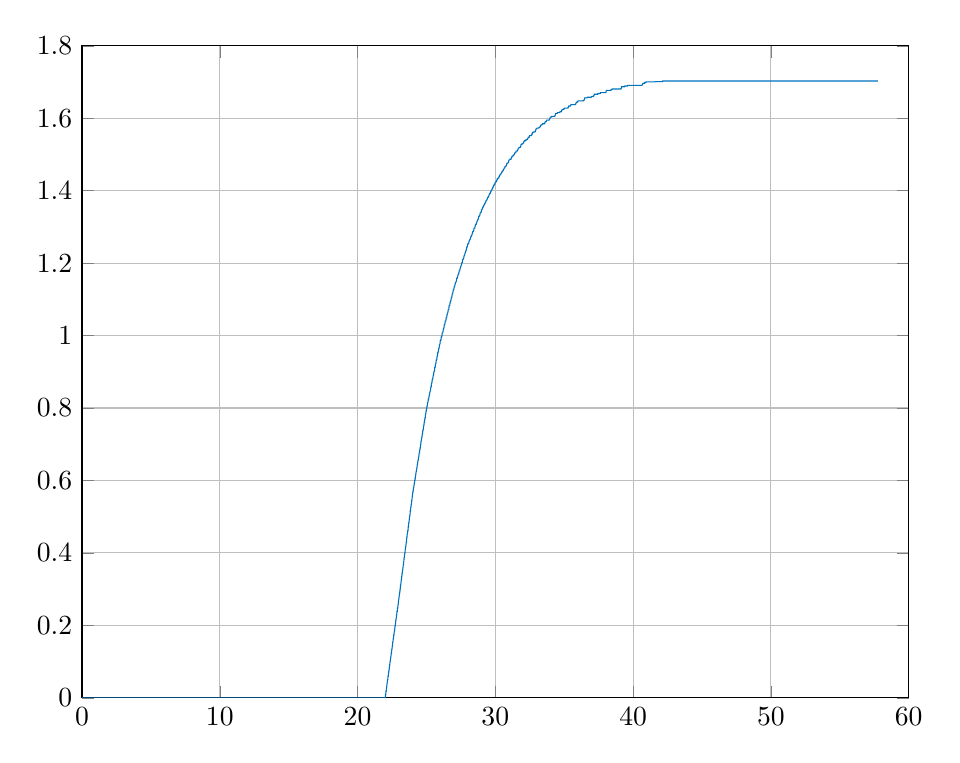
\begin{tikzpicture}

\begin{axis}[%
width=4.133in,
height=3.26in,
at={(0.693in,0.44in)},
scale only axis,
xmin=0,
xmax=60,
xmajorgrids,
ymin=0,
ymax=1.8,
ymajorgrids,
axis background/.style={fill=white}
]
\addplot [color=mycolor1,solid,forget plot]
  table[row sep=crcr]{%
0	0\\
0.0179118039999995	0\\
0.0330999039999992	0\\
0.048750436999999	0\\
0.0642097359999996	0\\
0.0798556380000003	0\\
0.0957486339999996	0\\
0.111709159	0\\
0.128792557	0\\
0.143668043	0\\
0.159576550999999	0\\
0.17766758	0\\
0.193047109999999	0\\
0.208477968999999	0\\
0.224017873	0\\
0.239796939999999	0\\
0.255747902999999	0\\
0.271881966	0\\
0.287974163999999	0\\
0.303747914999999	0\\
0.319712444	0\\
0.335854729	0\\
0.351747480999999	0\\
0.367800309999999	0\\
0.383669375	0\\
0.399585159	0\\
0.417663297999999	0\\
0.432459596999999	0\\
0.447867683	0\\
0.463873152999999	0\\
0.479865380999999	0\\
0.49588984	0\\
0.511904181	0\\
0.527763734999999	0\\
0.546094696999999	0\\
0.561157036999999	0\\
0.576219702	0\\
0.59172717	0\\
0.607834206999998	0\\
0.62366159	0\\
0.639634886	0\\
0.655714901999999	0\\
0.671695955	0\\
0.687711682	0\\
0.703612534	0\\
0.719698327	0\\
0.736002740999999	0\\
0.751813875	0\\
0.767909366999999	0\\
0.783930313999999	0\\
0.800050655999999	0\\
0.815986303999999	0\\
0.832080325999999	0\\
0.847988226	0\\
0.863913766999999	0\\
0.879877074999999	0\\
0.895577595999999	0\\
0.911638609999999	0\\
0.927615191	0\\
0.943710971999999	0\\
0.959570442	0\\
0.975702630999999	0\\
0.991700043	0\\
1.009233032	0\\
1.024242002	0\\
1.039625177	0\\
1.055652258	0\\
1.071681535	0\\
1.087710483	0\\
1.103754722	0\\
1.119887076	0\\
1.135594747	0\\
1.153729693	0\\
1.16916836	0\\
1.184356586	0\\
1.199697091	0\\
1.215674298	0\\
1.231682856	0\\
1.247679252	0\\
1.263696801	0\\
1.289572732	0\\
1.301487183	0\\
1.313492631	0\\
1.328740927	0\\
1.343984076	0\\
1.359730245	0\\
1.3758146	0\\
1.39162767	0\\
1.409796502	0\\
1.424920027	0\\
1.440080965	0\\
1.455833634	0\\
1.471752269	0\\
1.487773195	0\\
1.503740119	0\\
1.519802069	0\\
1.535762468	0\\
1.551716519	0\\
1.567808911	0\\
1.583746459	0\\
1.59974942	0\\
1.615872382	0\\
1.631697963	0\\
1.649047137	0\\
1.664102744	0\\
1.67974418	0\\
1.695760138	0\\
1.71173056	0\\
1.727680015	0\\
1.743756226	0\\
1.75974293	0\\
1.775762163	0\\
1.791757992	0\\
1.807767465	0\\
1.823749416	0\\
1.839725314	0\\
1.855729047	0\\
1.871830241	0\\
1.887669626	0\\
1.903622844	0\\
1.91976352	0\\
1.935733463	0\\
1.951787339	0\\
1.96784986	0\\
1.983760922	0\\
1.999939576	0\\
2.017738886	0\\
2.033098144	0\\
2.048565566	0\\
2.063921074	0\\
2.079841574	0\\
2.095839859	0\\
2.112164469	0\\
2.127597016	0\\
2.145672213	0\\
2.160545444	0\\
2.175783542	0\\
2.191777542	0\\
2.207728249	0\\
2.223755505	0\\
2.239721068	0\\
2.255758159	0\\
2.27174537	0\\
2.287828422	0\\
2.303741569	0\\
2.319736241	0\\
2.335766073	0\\
2.351754961	0\\
2.367692304	0\\
2.383743693	0\\
2.399636413	0\\
2.415701867	0\\
2.431671269	0\\
2.447618276	0\\
2.463595471	0\\
2.481712661	0\\
2.496685987	0\\
2.511589672	0\\
2.529687754	0\\
2.544618887	0\\
2.559816057	0\\
2.575729054	0\\
2.59173021	0\\
2.607775402	0\\
2.623950683	0\\
2.64041981	0\\
2.655715893	0\\
2.67157277	0\\
2.68757642	0\\
2.703720256	0\\
2.719739431	0\\
2.735704378	0\\
2.751758775	0\\
2.767730535	0\\
2.783797887	0\\
2.799767597	0\\
2.815714176	0\\
2.831713288	0\\
2.847718874	0\\
2.863683643	0\\
2.879642291	0\\
2.897697277	0\\
2.912492924	0\\
2.927737938	0\\
2.943795276	0\\
2.959766625	0\\
2.975871442	0\\
2.992099037	0\\
3.009693863	0\\
3.023716157	0\\
3.040118392	0\\
3.055924001	0\\
3.071909222	0\\
3.087919965	0\\
3.103938366	0\\
3.120334432	0\\
3.13700061	0\\
3.152441297	0\\
3.167885604	0\\
3.183928624	0\\
3.199777159	0\\
3.215747462	0\\
3.231893657	0\\
3.247758389	0\\
3.263776494	0\\
3.279734649	0\\
3.295738993	0\\
3.31411083	0\\
3.329270089	0\\
3.344457477	0\\
3.359778104	0\\
3.375782421	0\\
3.391591953	0\\
3.409730446	0\\
3.424901295	0\\
3.440078923	0\\
3.455908387	0\\
3.471667697	0\\
3.487579354	0\\
3.503841019	0\\
3.519709961	0\\
3.535807288	0\\
3.554187834	0\\
3.569433493	0\\
3.584727203	0\\
3.599879898	0\\
3.615773797	0\\
3.631774324	0\\
3.647630656	0\\
3.6637388	0\\
3.679862935	0\\
3.695661588	0\\
3.711743518	0\\
3.727712962	0\\
3.743711463	0\\
3.759656778	0\\
3.775853588	0\\
3.791816618	0\\
3.807959847	0\\
3.823973838	0\\
3.839775098	0\\
3.855904841	0\\
3.871847944	0\\
3.887789658	0\\
3.903742988	0\\
3.919629419	0\\
3.935711642	0\\
3.951699262	0\\
3.967729601	0\\
3.983730311	0\\
3.999758228	0\\
4.017143227	0\\
4.032110933	0\\
4.047655571	0\\
4.063630551	0\\
4.079590331	0\\
4.097794705	0\\
4.112840443	0\\
4.127919732	0\\
4.143715192	0\\
4.159674018	0\\
4.175702131	0\\
4.191690659	0\\
4.2076984	0\\
4.223611672	0\\
4.239615559	0\\
4.255610231	0\\
4.27161744	0\\
4.287753054	0\\
4.303854473	0\\
4.319837965	0\\
4.335867074	0\\
4.35188527	0\\
4.367909709	0\\
4.383730705	0\\
4.399728329	0\\
4.415860284	0\\
4.431726866	0\\
4.447690402	0\\
4.463704178	0\\
4.479863267	0\\
4.495879152	0\\
4.511874866	0\\
4.527914059	0\\
4.543856267	0\\
4.559714185	0\\
4.575718097	0\\
4.591790646	0\\
4.607656245	0\\
4.623797083	0\\
4.639806959	0\\
4.656027022	0\\
4.671864162	0\\
4.687786956	0\\
4.703919666	0\\
4.719850198	0\\
4.735720162	0\\
4.751872045	0\\
4.767844026	0\\
4.783792473	0\\
4.799594223	0\\
4.815879503	0\\
4.831853178	0\\
4.847872731	0\\
4.863882151	0\\
4.87983347	0\\
4.895714625	0\\
4.911703679	0\\
4.927723456	0\\
4.943780648	0\\
4.959809754	0\\
4.975920634	0\\
4.991814474	0\\
5.009259738	0\\
5.024627485	0\\
5.039848379	0\\
5.055630066	0\\
5.071673138	0\\
5.087746216	0\\
5.103860918	0\\
5.119667174	0\\
5.135550754	0\\
5.153771083	0\\
5.168833413	0\\
5.183875231	0\\
5.19977257	0\\
5.215708757	0\\
5.231688556	0\\
5.247682954	0\\
5.263902537	0\\
5.279697057	0\\
5.295745636	0\\
5.311777311	0\\
5.327679101	0\\
5.343795045	0\\
5.359832003	0\\
5.375956038	0\\
5.391700817	0\\
5.407728606	0\\
5.423841064	0\\
5.439783337	0\\
5.455783799	0\\
5.471773022	0\\
5.487689301	0\\
5.503596831	0\\
5.521804105	0\\
5.536927623	0\\
5.552073999	0\\
5.567949808	0\\
5.58372431	0\\
5.59976002	0\\
5.615702208	0\\
5.631833519	0\\
5.647631594	0\\
5.66374218	0\\
5.679729025	0\\
5.695717543	0\\
5.711647406	0\\
5.727745684	0\\
5.743659352	0\\
5.759711281	0\\
5.775738796	0\\
5.791720493	0\\
5.807713036	0\\
5.823709416	0\\
5.839698	0\\
5.855701833	0\\
5.871690786	0\\
5.887715486	0\\
5.903701534	0\\
5.919854128	0\\
5.935745466	0\\
5.951817901	0\\
5.967707178	0\\
5.983885325	0\\
5.99987674	0\\
6.017682554	0\\
6.033057142	0\\
6.048517754	0\\
6.063927266	0\\
6.079910361	0\\
6.095863289	0\\
6.111918528	0\\
6.127765295	0\\
6.143846708	0\\
6.159846952	0\\
6.175723326	0\\
6.191871276	0\\
6.207879854	0\\
6.223879091	0\\
6.239849609	0\\
6.255749	0\\
6.271695753	0\\
6.28772997	0\\
6.303733442	0\\
6.319700887	0\\
6.335763638	0\\
6.35171639	0\\
6.367701771	0\\
6.383857663	0\\
6.39968224	0\\
6.415696351	0\\
6.431692266	0\\
6.447700473	0\\
6.463715677	0\\
6.479740016	0\\
6.49576019	0\\
6.511735091	0\\
6.527715493	0\\
6.543701585	0\\
6.55969328	0\\
6.575672387	0\\
6.591693078	0\\
6.607716034	0\\
6.623837964	0\\
6.639729843	0\\
6.655702911	0\\
6.671724389	0\\
6.687818135	0\\
6.703901092	0\\
6.719892321	0\\
6.735868376	0\\
6.751880898	0\\
6.767798009	0\\
6.783724914	0\\
6.799823149	0\\
6.815728765	0\\
6.831964448	0\\
6.848084308	0\\
6.863860961	0\\
6.879776755	0\\
6.895783048	0\\
6.912001647	0\\
6.92792606	0\\
6.943876793	0\\
6.959877628	0\\
6.975856715	0\\
6.991861169	0\\
7.009693559	0\\
7.02491957	0\\
7.041321259	0\\
7.056979499	0\\
7.072373845	0\\
7.087908245	0\\
7.103897344	0\\
7.119910658	0\\
7.135863325	0\\
7.151918502	0\\
7.167887278	0\\
7.183845763	0\\
7.199943946	0\\
7.215878605	0\\
7.231923832	0\\
7.247876543	0\\
7.263944937	0\\
7.279923523	0\\
7.295886303	0\\
7.311892491	0\\
7.328546952	0\\
7.343954534	0\\
7.359905843	0\\
7.375810511	0\\
7.391707186	0\\
7.407665932	0\\
7.42369424	0\\
7.439698163	0\\
7.455894572	0\\
7.471987737	0\\
7.48788129	0\\
7.503728307	0\\
7.519679571	0\\
7.535717325	0\\
7.551922714	0\\
7.567940669	0\\
7.583847457	0\\
7.599724222	0\\
7.615939614	0\\
7.631924338	0\\
7.647869227	0\\
7.663875781	0\\
7.679887968	0\\
7.695872246	0\\
7.712029883	0\\
7.727823629	0\\
7.743717012	0\\
7.759693593	0\\
7.775699254	0\\
7.791713346	0\\
7.807695283	0\\
7.823858337	0\\
7.839886841	0\\
7.855742402	0\\
7.871736338	0\\
7.88775119	0\\
7.903890565	0\\
7.919691005	0\\
7.935719347	0\\
7.951811189	0\\
7.967643559	0\\
7.98375351	0\\
7.999752023	0\\
8.0172344	0\\
8.032501316	0\\
8.047637723	0\\
8.064008387	0\\
8.079890329	0\\
8.095943909	0\\
8.111866748	0\\
8.127792284	0\\
8.14377113	0\\
8.159872398	0\\
8.175859373	0\\
8.19188057	0\\
8.207744793	0\\
8.223646829	0\\
8.239699021	0\\
8.255700177	0\\
8.271754113	0\\
8.287822347	0\\
8.303729345	0\\
8.319706914	0\\
8.335718143	0\\
8.351746411	0\\
8.367740487	0\\
8.38370485	0\\
8.399856307	0\\
8.415710256	0\\
8.431708035	0\\
8.447868657	0\\
8.463921697	0\\
8.479767707	0\\
8.495879554	0\\
8.511934718	0\\
8.527904744	0\\
8.544041663	0\\
8.559885489	0\\
8.575874368	0\\
8.591872808	0\\
8.60772395	0\\
8.623806005	0\\
8.639760941	0\\
8.655905137	0\\
8.671887576	0\\
8.68786961	0\\
8.703890707	0\\
8.720257857	0\\
8.735929247	0\\
8.751905748	0\\
8.767909846	0\\
8.78385459	0\\
8.799874509	0\\
8.81583359	0\\
8.831717877	0\\
8.847698538	0\\
8.863700476	0\\
8.879781484	0\\
8.895712967	0\\
8.911792003	0\\
8.927860996	0\\
8.943896801	0\\
8.959865123	0\\
8.975883985	0\\
8.991911206	0\\
9.007731793	0\\
9.023915709	0\\
9.039890796	0\\
9.055831479	0\\
9.071689904	0\\
9.08785604	0\\
9.103896671	0\\
9.11973996	0\\
9.135812308	0\\
9.151856572	0\\
9.167694078	0\\
9.183822423	0\\
9.199635107	0\\
9.215768449	0\\
9.231860997	0\\
9.247786783	0\\
9.263889299	0\\
9.279792875	0\\
9.295761815	0\\
9.311779438	0\\
9.327953719	0\\
9.343892386	0\\
9.35974016	0\\
9.375845964	0\\
9.391769225	0\\
9.407621223	0\\
9.423829459	0\\
9.439598515	0\\
9.455897175	0\\
9.471797574	0\\
9.487734622	0\\
9.503754424	0\\
9.519864277	0\\
9.53576403	0\\
9.551704846	0\\
9.567757076	0\\
9.583762668	0\\
9.599740817	0\\
9.615699969	0\\
9.631913291	0\\
9.647748452	0\\
9.663720497	0\\
9.679720747	0\\
9.695744029	0\\
9.711697483	0\\
9.727765345	0\\
9.743725815	0\\
9.759728941	0\\
9.775734382	0\\
9.791826931	0\\
9.807746327	0\\
9.82371695	0\\
9.839969806	0\\
9.855889889	0\\
9.871885473	0\\
9.887870379	0\\
9.903941915	0\\
9.919940802	0\\
9.935812715	0\\
9.951856308	0\\
9.967908926	0\\
9.983885467	0\\
9.999870507	0\\
10.017515586	0\\
10.0330492	0\\
10.048517575	0\\
10.063966593	0\\
10.079901928	0\\
10.095876344	0\\
10.111721629	0\\
10.127886886	0\\
10.143933757	0\\
10.159870221	0\\
10.175857757	0\\
10.191729761	0\\
10.207701817	0\\
10.223753553	0\\
10.239764768	0\\
10.25575062	0\\
10.271769792	0\\
10.287769928	0\\
10.303671245	0\\
10.319759326	0\\
10.335801876	0\\
10.351792163	0\\
10.367868525	0\\
10.383722057	0\\
10.399643539	0\\
10.415919202	0\\
10.431763072	0\\
10.447756326	0\\
10.463703831	0\\
10.479751127	0\\
10.495690885	0\\
10.511704494	0\\
10.527721674	0\\
10.543649052	0\\
10.559795979	0\\
10.575710991	0\\
10.591701207	0\\
10.607691915	0\\
10.623792402	0\\
10.640954819	0\\
10.656163586	0\\
10.671952893	0\\
10.687835501	0\\
10.703741783	0\\
10.719677431	0\\
10.735707207	0\\
10.751734749	0\\
10.767734171	0\\
10.783758039	0\\
10.799733473	0\\
10.815718989	0\\
10.831687702	0\\
10.847805969	0\\
10.863925013	0\\
10.879838305	0\\
10.89588046	0\\
10.911907405	0\\
10.927931168	0\\
10.943852228	0\\
10.959890083	0\\
10.975881843	0\\
10.991753566	0\\
11.009408716	0\\
11.024746741	0\\
11.039924311	0\\
11.055677357	0\\
11.071685309	0\\
11.090163772	0\\
11.105435934	0\\
11.120604471	0\\
11.135821566	0\\
11.151807659	0\\
11.167915013	0\\
11.18363109	0\\
11.202018284	0\\
11.217192347	0\\
11.232399946	0\\
11.247780321	0\\
11.264021196	0\\
11.279791795	0\\
11.295852738	0\\
11.311744146	0\\
11.327677358	0\\
11.343765963	0\\
11.359748668	0\\
11.375836391	0\\
11.391635698	0\\
11.407760487	0\\
11.423705857	0\\
11.439779653	0\\
11.455756214	0\\
11.471626148	0\\
11.487732388	0\\
11.503738466	0\\
11.519737929	0\\
11.535729925	0\\
11.551744667	0\\
11.567777485	0\\
11.58373815	0\\
11.599893176	0\\
11.615916673	0\\
11.63182139	0\\
11.648136392	0\\
11.663866212	0\\
11.679835615	0\\
11.695885943	0\\
11.712047428	0\\
11.727712559	0\\
11.743710333	0\\
11.759691254	0\\
11.775706086	0\\
11.792020252	0\\
11.807652267	0\\
11.823691024	0\\
11.839700725	0\\
11.855811039	0\\
11.871717706	0\\
11.88777132	0\\
11.903687416	0\\
11.919764595	0\\
11.935799487	0\\
11.951755317	0\\
11.96777037	0\\
11.983826426	0\\
11.999702692	0\\
12.017246742	0\\
12.032372119	0\\
12.047717255	0\\
12.063725633	0\\
12.079728583	0\\
12.095737984	0\\
12.111701145	0\\
12.127716704	0\\
12.144029687	0\\
12.159859786	0\\
12.175727555	0\\
12.191705014	0\\
12.207700157	0\\
12.22366685	0\\
12.239697218	0\\
12.255797724	0\\
12.271697056	0\\
12.287720643	0\\
12.303666765	0\\
12.319667195	0\\
12.335745757	0\\
12.351730897	0\\
12.367729473	0\\
12.38357457	0\\
12.401623232	0\\
12.416410069	0\\
12.431831755	0\\
12.447728732	0\\
12.463697906	0\\
12.479777846	0\\
12.495915146	0\\
12.512208048	0\\
12.527857849	0\\
12.543877172	0\\
12.559855812	0\\
12.575873782	0\\
12.591844595	0\\
12.607836892	0\\
12.623853183	0\\
12.639589795	0\\
12.655821008	0\\
12.671754236	0\\
12.687703966	0\\
12.703690309	0\\
12.719816759	0\\
12.735880358	0\\
12.751723651	0\\
12.767698073	0\\
12.783679209	0\\
12.79964918	0\\
12.81586833	0\\
12.831968837	0\\
12.847852533	0\\
12.863747779	0\\
12.87988732	0\\
12.895600268	0\\
12.911678399	0\\
12.927869636	0\\
12.943837738	0\\
12.960029557	0\\
12.975933228	0\\
12.991754436	0\\
13.009294434	0\\
13.024322632	0\\
13.039722802	0\\
13.055636918	0\\
13.071654545	0\\
13.08770087	0\\
13.103691998	0\\
13.119853478	0\\
13.135790827	0\\
13.151787091	0\\
13.167875315	0\\
13.183871761	0\\
13.199760673	0\\
13.215888477	0\\
13.23186162	0\\
13.247863433	0\\
13.263904044	0\\
13.279839722	0\\
13.2958941	0\\
13.311839244	0\\
13.327777037	0\\
13.343762248	0\\
13.359696027	0\\
13.375700341	0\\
13.391771172	0\\
13.407816615	0\\
13.423714866	0\\
13.439682136	0\\
13.455676487	0\\
13.471863855	0\\
13.487791876	0\\
13.503781471	0\\
13.51969948	0\\
13.535711667	0\\
13.551697699	0\\
13.567663796	0\\
13.583669087	0\\
13.599911746	0\\
13.615941863	0\\
13.631871423	0\\
13.649431103	0\\
13.664349895	0\\
13.679802113	0\\
13.695696046	0\\
13.711768595	0\\
13.727890755	0\\
13.743981605	0\\
13.759871655	0\\
13.775946624	0\\
13.791879737	0\\
13.807824004	0\\
13.82354873	0\\
13.839966996	0\\
13.855907215	0\\
13.872018742	0\\
13.887689072	0\\
13.903547537	0\\
13.919845917	0\\
13.936194005	0\\
13.951889689	0\\
13.967712671	0\\
13.983613422	0\\
13.999691828	0\\
14.017205561	0\\
14.032349641	0\\
14.047684003	0\\
14.063872464	0\\
14.079724513	0\\
14.095706075	0\\
14.111643026	0\\
14.128105523	0\\
14.143591773	0\\
14.16178708	0\\
14.176883677	0\\
14.192164733	0\\
14.207702806	0\\
14.223694686	0\\
14.239851696	0\\
14.255875278	0\\
14.271858094	0\\
14.287871894	0\\
14.30391918	0\\
14.319883127	0\\
14.336746612	0\\
14.352219292	0\\
14.367901706	0\\
14.383896208	0\\
14.399788057	0\\
14.41577872	0\\
14.43194457	0\\
14.447851242	0\\
14.46372942	0\\
14.479707354	0\\
14.495708766	0\\
14.511717776	0\\
14.527660385	0\\
14.543876323	0\\
14.559911421	0\\
14.575894903	0\\
14.591883566	0\\
14.607884863	0\\
14.623719909	0\\
14.639609542	0\\
14.655752866	0\\
14.671923557	0\\
14.687964796	0\\
14.703733953	0\\
14.719740047	0\\
14.73569278	0\\
14.751933099	0\\
14.767874135	0\\
14.783699671	0\\
14.799769661	0\\
14.81572787	0\\
14.831684626	0\\
14.847691816	0\\
14.86370698	0\\
14.880019853	0\\
14.895766127	0\\
14.911838046	0\\
14.927887986	0\\
14.943878914	0\\
14.959902367	0\\
14.97584461	0\\
14.991720939	0\\
15.009126537	0\\
15.0242078	0\\
15.039844861	0\\
15.055865983	0\\
15.071731282	0\\
15.087724266	0\\
15.103708078	0\\
15.119691544	0\\
15.135774552	0\\
15.15163189	0\\
15.167734655	0\\
15.183834089	0\\
15.199784505	0\\
15.215698252	0\\
15.231874026	0\\
15.2481038	0\\
15.263895197	0\\
15.279825122	0\\
15.295896338	0\\
15.311809956	0\\
15.327865741	0\\
15.343860529	0\\
15.359872184	0\\
15.375869216	0\\
15.3917786	0\\
15.407866568	0\\
15.423807659	0\\
15.439718521	0\\
15.455862151	0\\
15.471905905	0\\
15.487874026	0\\
15.503798012	0\\
15.519844982	0\\
15.53591262	0\\
15.55206762	0\\
15.567705855	0\\
15.58367997	0\\
15.599709361	0\\
15.615956044	0\\
15.631898337	0\\
15.647816846	0\\
15.663853819	0\\
15.679866387	0\\
15.695723141	0\\
15.711869296	0\\
15.727922937	0\\
15.743860379	0\\
15.759845128	0\\
15.776012231	0\\
15.791918588	0\\
15.807882154	0\\
15.823892011	0\\
15.839798557	0\\
15.855852123	0\\
15.871870348	0\\
15.887846907	0\\
15.903923601	0\\
15.919878947	0\\
15.935726635	0\\
15.95169441	0\\
15.967883117	0\\
15.983904319	0\\
15.999887725	0\\
16.017617192	0\\
16.032884211	0\\
16.048349103	0\\
16.063765675	0\\
16.079957017	0\\
16.095858478	0\\
16.111853456	0\\
16.127862811	0\\
16.143847945	0\\
16.159744335	0\\
16.175717344	0\\
16.191665721	0\\
16.207702668	0\\
16.223577439	0\\
16.239874606	0\\
16.255880273	0\\
16.271887438	0\\
16.287845928	0\\
16.303898316	0\\
16.319873183	0\\
16.336931865	0\\
16.352462691	0\\
16.367841177	0\\
16.383755758	0\\
16.39968624	0\\
16.415879161	0\\
16.431779022	0\\
16.447869304	0\\
16.463873996	0\\
16.479937754	0\\
16.495853277	0\\
16.511878508	0\\
16.528071479	0\\
16.543920406	0\\
16.559947512	0\\
16.575858178	0\\
16.591884722	0\\
16.607935096	0\\
16.623873099	0\\
16.639860599	0\\
16.655778127	0\\
16.671706574	0\\
16.687615455	0\\
16.703883182	0\\
16.719875529	0\\
16.735907089	0\\
16.751875166	0\\
16.767879414	0\\
16.783874066	0\\
16.79984752	0\\
16.81586113	0\\
16.83172235	0\\
16.847697793	0\\
16.863874102	0\\
16.879891119	0\\
16.895595481	0\\
16.913822688	0\\
16.929289554	0\\
16.944775602	0\\
16.960260245	0\\
16.97590725	0\\
16.99185899	0\\
17.009827788	0\\
17.025435118	0\\
17.040998914	0\\
17.056208362	0\\
17.071714487	0\\
17.087697363	0\\
17.103857565	0\\
17.119885246	0\\
17.135830592	0\\
17.151824334	0\\
17.167756577	0\\
17.183855109	0\\
17.19993551	0\\
17.215960822	0\\
17.231718903	0\\
17.247701542	0\\
17.263715854	0\\
17.279702818	0\\
17.295702181	0\\
17.31166892	0\\
17.327768935	0\\
17.343750618	0\\
17.359730686	0\\
17.375723048	0\\
17.39162808	0\\
17.407577538	0\\
17.426021642	0\\
17.441645674	0\\
17.456755036	0\\
17.471760412	0\\
17.487709767	0\\
17.50369187	0\\
17.519871265	0\\
17.536064196	0\\
17.55186102	0\\
17.567853156	0\\
17.583891623	0\\
17.599857604	0\\
17.615868844	0\\
17.632084411	0\\
17.647645068	0\\
17.66370948	0\\
17.679693593	0\\
17.695707834	0\\
17.711801586	0\\
17.727693179	0\\
17.743724374	0\\
17.759667389	0\\
17.775882735	0\\
17.791897959	0\\
17.807851979	0\\
17.823897551	0\\
17.839895436	0\\
17.855876296	0\\
17.871872917	0\\
17.887806141	0\\
17.90383978	0\\
17.919800987	0\\
17.935864003	0\\
17.951623751	0\\
17.968873809	0\\
17.984128818	0\\
17.999642604	0\\
18.017873375	0\\
18.033269291	0\\
18.048411626	0\\
18.063734134	0\\
18.079746832	0\\
18.095612544	0\\
18.111811268	0\\
18.127933342	0\\
18.145389837	0\\
18.160632541	0\\
18.175741744	0\\
18.191763768	0\\
18.207694513	0\\
18.223724233	0\\
18.239790513	0\\
18.255764348	0\\
18.271715527	0\\
18.287776734	0\\
18.303725277	0\\
18.319848545	0\\
18.335898157	0\\
18.351863793	0\\
18.367917343	0\\
18.383875868	0\\
18.399630798	0\\
18.415582664	0\\
18.433571702	0\\
18.44862872	0\\
18.463687361	0\\
18.47960983	0\\
18.495701191	0\\
18.513972835	0\\
18.529287592	0\\
18.544704095	0\\
18.560097279	0\\
18.576031709	0\\
18.5917413	0\\
18.607656141	0\\
18.623839386	0\\
18.639831079	0\\
18.655585027	0\\
18.673627298	0\\
18.688690866	0\\
18.703934091	0\\
18.719701518	0\\
18.735665515	0\\
18.751876286	0\\
18.767872622	0\\
18.783859256	0\\
18.799917206	0\\
18.815857374	0\\
18.831946782	0\\
18.847854887	0\\
18.864023157	0\\
18.879899692	0\\
18.895639341	0\\
18.911732948	0\\
18.927842083	0\\
18.943842358	0\\
18.959791006	0\\
18.975855204	0\\
18.991883939	0\\
19.009772454	0\\
19.025223887	0\\
19.040585245	0\\
19.056239345	0\\
19.07188861	0\\
19.08786718	0\\
19.103794129	0\\
19.119839942	0\\
19.135818492	0\\
19.152066213	0\\
19.167844349	0\\
19.183784272	0\\
19.199853926	0\\
19.215665	0\\
19.231715277	0\\
19.247870388	0\\
19.263891382	0\\
19.279961733	0\\
19.295675195	0\\
19.311811079	0\\
19.327691292	0\\
19.343817003	0\\
19.359833071	0\\
19.375764927	0\\
19.391699555	0\\
19.407698209	0\\
19.423676103	0\\
19.439739526	0\\
19.455675759	0\\
19.472028913	0\\
19.48769148	0\\
19.503791884	0\\
19.519706164	0\\
19.53573347	0\\
19.551766594	0\\
19.567758731	0\\
19.583834146	0\\
19.599614216	0\\
19.61786122	0\\
19.633015448	0\\
19.648347818	0\\
19.663652471	0\\
19.679792375	0\\
19.695648628	0\\
19.711736541	0\\
19.727739435	0\\
19.743762299	0\\
19.759774309	0\\
19.775828987	0\\
19.791677672	0\\
19.807809584	0\\
19.823730208	0\\
19.839675374	0\\
19.855655555	0\\
19.871713053	0\\
19.887757973	0\\
19.903705895	0\\
19.919889205	0\\
19.935762727	0\\
19.95181536	0\\
19.968041089	0\\
19.983702619	0\\
20.000001615	0\\
20.017602735	0\\
20.032825448	0\\
20.048073124	0\\
20.063643053	0\\
20.081935157	0\\
20.097175633	0\\
20.112482884	0\\
20.127833676	0\\
20.143682536	0\\
20.159609123	0\\
20.177580923	0\\
20.192555477	0\\
20.207851792	0\\
20.223730351	0\\
20.239712936	0\\
20.255914136	0\\
20.271907269	0\\
20.287859715	0\\
20.303909803	0\\
20.319853935	0\\
20.335867049	0\\
20.352394618	0\\
20.367729981	0\\
20.383780751	0\\
20.399599573	0\\
20.417663093	0\\
20.433217112	0\\
20.448750353	0\\
20.464386763	0\\
20.480035888	0\\
20.495896787	0\\
20.51190077	0\\
20.528153772	0\\
20.543997918	0\\
20.559903713	0\\
20.575872206	0\\
20.591842207	0\\
20.607949815	0\\
20.623882531	0\\
20.639687998	0\\
20.655591043	0\\
20.673702826	0\\
20.688875968	0\\
20.703918924	0\\
20.719707444	0\\
20.735704196	0\\
20.751719219	0\\
20.767691104	0\\
20.783756967	0\\
20.799693137	0\\
20.815716519	0\\
20.831641805	0\\
20.847637385	0\\
20.863640346	0\\
20.879609913	0\\
20.895588428	0\\
20.913686254	0\\
20.929125203	0\\
20.944540949	0\\
20.959997687	0\\
20.976018203	0\\
20.991795266	0\\
21.00943077	0\\
21.024805262	0\\
21.040425005	0\\
21.055888213	0\\
21.071865846	0\\
21.087737249	0\\
21.103964423	0\\
21.119876883	0\\
21.135792191	0\\
21.151650917	0\\
21.169683786	0\\
21.185140162	0\\
21.200718478	0\\
21.216276723	0\\
21.232058914	0\\
21.247877302	0\\
21.263886176	0\\
21.279725656	0\\
21.295873891	0\\
21.311879423	0\\
21.32780589	0\\
21.343630782	0\\
21.359810854	0\\
21.375607683	0\\
21.391593474	0\\
21.407738943	0\\
21.423597912	0\\
21.439762866	0\\
21.455828438	0\\
21.471839437	0\\
21.48771552	0\\
21.503705517	0\\
21.519708799	0\\
21.535732887	0\\
21.551597562	0\\
21.567702702	0\\
21.583695077	0\\
21.599759414	0\\
21.615729264	0\\
21.631746655	0\\
21.647687553	0\\
21.665841085	0\\
21.681128054	0\\
21.696538377	0\\
21.711885327	0\\
21.727871389	0\\
21.743884798	0\\
21.759960945	0\\
21.775867082	0\\
21.791850939	0\\
21.807895058	0\\
21.82388092	0\\
21.839842532	0\\
21.855957647	0\\
21.871880817	0\\
21.887821782	0\\
21.903604482	0\\
21.921751857	0\\
21.937330842	0\\
21.95276558	0\\
21.968163561	0\\
21.983925276	0\\
21.999933012	0.00196318773208936\\
22.017373349	0.00196318773208936\\
22.032437439	0.00981195926176576\\
22.048008174	0.00981195926176576\\
22.063886287	0.0180426914289087\\
22.079976045	0.0184366372966776\\
22.095839965	0.0270575516131847\\
22.111878376	0.0290183694663439\\
22.127857012	0.0349063231428611\\
22.143764697	0.0407924421716012\\
22.159584096	0.0427550946725375\\
22.175843704	0.0486412137012777\\
22.191937716	0.0506038662022139\\
22.207885717	0.0584526377318903\\
22.223897227	0.0588345983693568\\
22.239724886	0.067464757162202\\
22.255702404	0.0678494585536328\\
22.271700694	0.0756982300833092\\
22.287707864	0.0756982300833092\\
22.30368191	0.0835470016129856\\
22.319879657	0.0855078194661448\\
22.335927604	0.091395773142662\\
22.351888069	0.0972818921714022\\
22.367876231	0.099626505309805\\
22.383905692	0.105906570206314\\
22.399605249	0.108641365494081\\
22.417814053	0.114527484522821\\
22.432966148	0.116490137023757\\
22.448326581	0.124338908553434\\
22.46382437	0.124338908553434\\
22.479897067	0.13218768008311\\
22.495887574	0.134148497936269\\
22.511927935	0.140036451612787\\
22.527905723	0.142773175971181\\
22.543850512	0.149048571043098\\
22.559711551	0.155319391463269\\
22.575695995	0.157282043964205\\
22.591703481	0.163168162992946\\
22.607865986	0.165130815493882\\
22.623905352	0.172979587023558\\
22.639873638	0.172979587023558\\
22.655597611	0.180828358553235\\
22.671770789	0.18160426505847\\
22.68765072	0.189840477983546\\
22.703651772	0.190225179374977\\
22.719548501	0.198073950904654\\
22.73552303	0.200034768757813\\
22.753852199	0.20592272243433\\
22.769442001	0.21180884146307\\
22.784860385	0.213771493964006\\
22.80031133	0.219657612992747\\
22.815900113	0.221620265493683\\
22.831871457	0.230244943528595\\
22.847950685	0.230632384923995\\
22.863873665	0.238865857845102\\
22.879836284	0.238865857845102\\
22.895676329	0.246714629374778\\
22.911589822	0.246714629374778\\
22.929679006	0.254563400904455\\
22.94522009	0.256524218757614\\
22.960864018	0.262412172434131\\
22.976430524	0.269074197968107\\
22.99192109	0.271424291864443\\
23.009444665	0.277695112284614\\
23.024899143	0.28161837610036\\
23.040560771	0.285541307397011\\
23.056173588	0.291427758944846\\
23.071970893	0.291427758944846\\
23.087892554	0.30163211428488\\
23.10381388	0.30163211428488\\
23.119756253	0.311441497129367\\
23.135816689	0.311441497129367\\
23.15159341	0.317718985608596\\
23.169774683	0.324374839189298\\
23.184841283	0.326335657042457\\
23.199949541	0.334568923425215\\
23.21585219	0.334568923425215\\
23.231747146	0.344773278765249\\
23.247770142	0.344773278765249\\
23.263875405	0.35065682137671\\
23.279748746	0.354582661609736\\
23.295925401	0.358505386368037\\
23.311892881	0.364392044454222\\
23.327791786	0.366746601636801\\
23.343895766	0.374595373166477\\
23.359865406	0.377325386514154\\
23.376237448	0.385951790744682\\
23.392914918	0.387914443245619\\
23.409325726	0.393797985857079\\
23.424438696	0.397723826090105\\
23.439677566	0.399684437404915\\
23.455687151	0.407533208934591\\
23.47193035	0.409493820249401\\
23.487895421	0.415379939278141\\
23.503767272	0.419303203093888\\
23.519783786	0.423620080258307\\
23.53583242	0.429901504301691\\
23.551810515	0.430670906334557\\
23.56774802	0.440864990570474\\
23.583839679	0.442825601885284\\
23.599761576	0.450674373414961\\
23.615682842	0.45263498472977\\
23.631840689	0.456557916026421\\
23.648958896	0.462444367574257\\
23.663995387	0.462444367574257\\
23.679796736	0.472648722914291\\
23.69563078	0.47304266878206\\
23.714069558	0.482852051626546\\
23.729307616	0.483621453659413\\
23.74463454	0.489504996270873\\
23.759922693	0.49381553789533\\
23.776051156	0.49969908050679\\
23.791915561	0.503624920739816\\
23.80761041	0.505585532054626\\
23.825761052	0.51578988739466\\
23.83958801	0.51578988739466\\
23.855584616	0.52363661773821\\
23.871765673	0.525599270239146\\
23.887675353	0.531876758718376\\
23.903594072	0.535802598951402\\
23.919599123	0.538532612299078\\
23.937696905	0.546381383828754\\
23.953388856	0.548726696534995\\
23.968548367	0.555007788059283\\
23.983862812	0.558931051875029\\
23.999751269	0.56481459448649\\
24.017393212	0.568740411274753\\
24.032373421	0.568740411274753\\
24.047705221	0.57658660638715\\
24.063705285	0.578549494152311\\
24.079688968	0.58090405133489\\
24.09569277	0.58678950030836\\
24.111704581	0.590712719274231\\
24.127700871	0.59110084555281\\
24.143816858	0.597764120585916\\
24.15958336	0.602073327009397\\
24.177831164	0.602073473024276\\
24.192877192	0.609919263305675\\
24.207904493	0.611882262296056\\
24.22385778	0.615804790775037\\
24.240170493	0.621690845739699\\
24.255825257	0.623651421981797\\
24.271783446	0.627573988106171\\
24.287888862	0.631499090812012\\
24.303858118	0.633459595842737\\
24.319622221	0.638170868762204\\
24.335799544	0.644056448257627\\
24.35201549	0.644056448257627\\
24.367777661	0.650328862925957\\
24.383785148	0.654638397853211\\
24.399616088	0.655025496789313\\
24.415791139	0.66090881692735\\
24.431778434	0.664833515698826\\
24.447850987	0.666794127013636\\
24.463812378	0.672678606526795\\
24.479739858	0.676601726969124\\
24.495784584	0.676601726969124\\
24.511626566	0.682880898898203\\
24.527714529	0.686803879928226\\
24.543793959	0.687197825795995\\
24.559728072	0.695042356106134\\
24.575754736	0.697004586229732\\
24.591742758	0.701317771204806\\
24.607732329	0.707589035820639\\
24.623641281	0.709938312490638\\
24.641714596	0.713860428029127\\
24.656703064	0.717784595930187\\
24.671735803	0.719745258439301\\
24.687720582	0.724062278105101\\
24.703694762	0.729946912576438\\
24.719723953	0.729946755204621\\
24.735700965	0.737791051901741\\
24.751875359	0.739753232936628\\
24.767908267	0.740146803125457\\
24.78387458	0.747990963325121\\
24.799830143	0.749953076768612\\
24.815918016	0.752306186822398\\
24.831775177	0.758189425138732\\
24.847721023	0.762499866088765\\
24.863895848	0.762890164976821\\
24.879800677	0.769168508436715\\
24.895836146	0.773091097832921\\
24.911798124	0.773091087188229\\
24.927871499	0.780934842081855\\
24.943941381	0.782896752392553\\
24.959781503	0.786818250287181\\
24.975749715	0.792701982369503\\
24.991731153	0.792701982369503\\
25.00911015	0.797017357405241\\
25.024216615	0.800939307522291\\
25.039745321	0.804861761317339\\
25.055747486	0.805256049406382\\
25.071705655	0.811533954815679\\
25.087692624	0.815456408610727\\
25.103749322	0.816236427391638\\
25.11974028	0.818197176458408\\
25.135735243	0.824079971620198\\
25.151598312	0.826041814100436\\
25.169834947	0.826041814100436\\
25.185081328	0.831923992335175\\
25.200361252	0.833885358328996\\
25.215784369	0.835847200809234\\
25.231873675	0.839768561190814\\
25.247867224	0.843690745037793\\
25.263785379	0.845652587518031\\
25.279857862	0.84800714470061\\
25.295906035	0.850362866262928\\
25.311900401	0.856246892590146\\
25.329255826	0.858207503904956\\
25.3447529	0.858601791993998\\
25.360167247	0.866834623823442\\
25.37592143	0.868795989817263\\
25.39182464	0.869187197483707\\
25.407660257	0.873108557865287\\
25.423819531	0.878992584192505\\
25.439752348	0.878992584192505\\
25.455729811	0.880953195507315\\
25.471737708	0.884875787054323\\
25.487624656	0.888797970901302\\
25.503734303	0.890758582216112\\
25.519750263	0.890758582216112\\
25.535740399	0.898998330105648\\
25.551869662	0.900958941420458\\
25.567892263	0.901352887288227\\
25.583845631	0.903313636354997\\
25.599871849	0.911158273997024\\
25.615797284	0.911158273997024\\
25.631847863	0.911552562086067\\
25.64773911	0.919396582801044\\
25.664781561	0.921746759909332\\
25.679929902	0.922137967575776\\
25.695804847	0.926059327957355\\
25.711875215	0.931943354284573\\
25.727606334	0.933903965599383\\
25.745750759	0.933903965599383\\
25.761221991	0.938221529641939\\
25.776361502	0.944104324803729\\
25.792008005	0.944104324803729\\
25.807655346	0.944104324803729\\
25.823694384	0.953909711512526\\
25.839749722	0.953909711512526\\
25.855761911	0.954303657380295\\
25.871763548	0.958225017761875\\
25.889133104	0.964109044089093\\
25.904173128	0.964109044089093\\
25.919706014	0.966463943492945\\
25.935900423	0.970386535039954\\
25.951810258	0.9746975300014\\
25.970288391	0.97665814131621\\
25.985430777	0.977444321478202\\
26.000686898	0.98528909687219\\
26.015838565	0.987249708187\\
26.032150555	0.987249708187\\
26.047890424	0.987249673973547\\
26.063914217	0.991171034355127\\
26.079758384	0.997054991895956\\
26.09570337	0.997054882623389\\
26.111654858	0.997054882623389\\
26.127792524	1.00097624300497\\
26.143803177	1.00685994724855\\
26.159684265	1.00685994724855\\
26.175721223	1.0072549197441\\
26.191699332	1.00921568246054\\
26.207694305	1.01313779752113\\
26.224005479	1.01706018235062\\
26.239683175	1.0190208696973\\
26.255764852	1.01941515778634\\
26.271719559	1.02177087934866\\
26.287670702	1.02765456114667\\
26.303786782	1.03000398411861\\
26.319817026	1.03039519178505\\
26.335684389	1.03039519178505\\
26.351658579	1.0362779122392\\
26.367613061	1.04020008981366\\
26.383653418	1.04020008981366\\
26.39957372	1.04020000822404\\
26.4176804	1.04412136860562\\
26.432619669	1.05000484296946\\
26.447618205	1.05000468559205\\
26.465715642	1.05000468559205\\
26.480758096	1.05196529690686\\
26.495773199	1.05784737530847\\
26.511726782	1.05980921778871\\
26.528126306	1.06176982910352\\
26.543652518	1.06256227131088\\
26.559611364	1.06452302037765\\
26.575727267	1.0704062867699\\
26.591615011	1.07236692415931\\
26.607694554	1.07276121224835\\
26.6236173	1.07276121224835\\
26.639750411	1.08060392709867\\
26.655586443	1.08256571943566\\
26.673713939	1.08295453055013\\
26.689123947	1.08334573821658\\
26.703600618	1.08726704168035\\
26.719574477	1.09315009956365\\
26.735625125	1.09315009956365\\
26.751671293	1.09314996624889\\
26.767626696	1.09707132663047\\
26.783691393	1.09903269262429\\
26.799616152	1.10295410506029\\
26.815583459	1.1049147163751\\
26.831592495	1.10530968887064\\
26.8477035	1.10727022121236\\
26.863614197	1.11315307004941\\
26.879656769	1.11511368136422\\
26.895627417	1.1155134919483\\
26.911638717	1.11747424101507\\
26.929675708	1.1213951775704\\
26.944542145	1.12531760313367\\
26.959620467	1.12531760313367\\
26.975606522	1.12571189122271\\
26.991679932	1.12963325160429\\
27.009325575	1.1335540131203\\
27.024672085	1.13551585560054\\
27.039772082	1.1355158027481\\
27.055576274	1.13825636387826\\
27.073773046	1.14021711294502\\
27.087686803	1.14217835084812\\
27.103766637	1.14609962410785\\
27.119747355	1.14609962410785\\
27.135673422	1.1480600974318\\
27.151592043	1.14845589299841\\
27.167742713	1.15041664206518\\
27.18368919	1.15433743883848\\
27.199769425	1.15825974878113\\
27.215656017	1.15825974878113\\
27.231775466	1.15825974878113\\
27.247679593	1.16022055466716\\
27.263708878	1.16218192066098\\
27.279752998	1.16610161733025\\
27.295744146	1.16806344096139\\
27.311706034	1.16846422896072\\
27.327743874	1.16846422896072\\
27.343886837	1.17238508001623\\
27.359816947	1.17434644601005\\
27.375835148	1.17826771926978\\
27.391783645	1.17826761810926\\
27.407807082	1.17866190619831\\
27.423842351	1.1806219641165\\
27.439773335	1.18454390204967\\
27.455748401	1.18650333282915\\
27.471813728	1.18846517530939\\
27.487734398	1.19042516378431\\
27.503857791	1.191603323156\\
27.519708103	1.19356407222277\\
27.538214117	1.19552543821659\\
27.553370169	1.19748495120364\\
27.568491367	1.20140664309312\\
27.583827848	1.20140664309312\\
27.599690227	1.20140664902314\\
27.615764794	1.20336739808991\\
27.631741164	1.20924797465007\\
27.647813231	1.21120974666338\\
27.663751631	1.21120974666338\\
27.679888946	1.21120974666338\\
27.695723385	1.21317041848866\\
27.711754359	1.21513005885165\\
27.727778588	1.21905085562495\\
27.743764806	1.221413332287\\
27.759772553	1.221413332287\\
27.775867051	1.22337290284851\\
27.792188688	1.22533365191528\\
27.807770364	1.22729478739617\\
27.823823699	1.23121606065589\\
27.839777308	1.23121606065589\\
27.855773419	1.23397033011689\\
27.871734409	1.23397033011689\\
27.887769688	1.23593107918366\\
27.903631334	1.23985190365471\\
27.919599413	1.24377310693389\\
27.935716209	1.24377310693389\\
27.951797472	1.24416426529203\\
27.967904935	1.24651382547326\\
27.983736184	1.24847519146708\\
27.999845543	1.25239378657155\\
28.017308762	1.25435562905179\\
28.03260528	1.25435562905179\\
28.047899187	1.25435562905179\\
28.063784922	1.25435543096061\\
28.080161859	1.25827540068617\\
28.095754546	1.26023676667999\\
28.111639111	1.26219585158134\\
28.127783089	1.26415769406158\\
28.143811881	1.26415769406158\\
28.159626581	1.26415741033815\\
28.175782996	1.26611663099694\\
28.191914758	1.26807738006371\\
28.207699598	1.27003845450826\\
28.223832019	1.27239976084975\\
28.239798413	1.27436160332999\\
28.255826144	1.27436157566575\\
28.271830312	1.27672261022445\\
28.287833413	1.27672261022445\\
28.303694583	1.27868332372922\\
28.31973381	1.28064468972304\\
28.335761768	1.28260369972401\\
28.351728527	1.28652476286304\\
28.367600675	1.28691893715371\\
28.383596705	1.28691893715371\\
28.401790716	1.28691893715371\\
28.416845683	1.28887956446467\\
28.432029103	1.29084093045849\\
28.447791358	1.29475902038133\\
28.464752811	1.29672066269036\\
28.48017055	1.29672066269036\\
28.495756817	1.2971118703568\\
28.511613485	1.29711166216851\\
28.527743108	1.30142044300854\\
28.543612382	1.30338180900236\\
28.559863194	1.30534025050811\\
28.578263552	1.30730209298835\\
28.593502214	1.30730209298835\\
28.608684512	1.30730179812892\\
28.623934912	1.30926101878772\\
28.639623388	1.31122176785449\\
28.655864391	1.31318283091215\\
28.671939755	1.31514134728968\\
28.687829622	1.31710318976992\\
28.703850547	1.31750500366982\\
28.719830356	1.31946384255944\\
28.735702402	1.31946384255944\\
28.751674034	1.32142459162621\\
28.767782589	1.32338556771449\\
28.783829138	1.32574985891756\\
28.799930262	1.32967092205659\\
28.815841239	1.32967079493379\\
28.831897084	1.32967079493379\\
28.847879714	1.32967079493379\\
28.86391456	1.33163140866937\\
28.879891524	1.33359277466319\\
28.895744527	1.33751022831642\\
28.911609324	1.3394718562622\\
28.927790562	1.33986614435124\\
28.943872461	1.33986614435124\\
28.959786669	1.33986592154876\\
28.975788715	1.34182667061553\\
28.991826244	1.34574706238324\\
29.009409119	1.34770485114352\\
29.024903635	1.34770459804726\\
29.040048649	1.34966610148647\\
29.055692462	1.35005743008022\\
29.071686002	1.35005721473121\\
29.087693071	1.35397676592458\\
29.103608615	1.35397646654947\\
29.119716412	1.35632715234278\\
29.135691766	1.35632721094235\\
29.151773014	1.35828478116485\\
29.167776641	1.35828431135331\\
29.183614094	1.36064869529966\\
29.199668108	1.36260766184087\\
29.215711922	1.36260717525454\\
29.231695964	1.36456760543888\\
29.247688551	1.36456755408137\\
29.263731488	1.36652816270006\\
29.279836229	1.36652791585648\\
29.29586374	1.36848548101737\\
29.311934129	1.37044378472894\\
29.327881243	1.37240488698463\\
29.343907727	1.37240463360923\\
29.359740988	1.37240463360923\\
29.37572247	1.374364115325\\
29.39188574	1.37477400822832\\
29.407606944	1.3767346804534\\
29.423637284	1.37869291600507\\
29.439630775	1.38065004829542\\
29.455644189	1.38064982407296\\
29.471629763	1.38261047418542\\
29.487639389	1.38261007220391\\
29.503895665	1.38260983996438\\
29.519925527	1.38456937008003\\
29.53593159	1.38652978061991\\
29.551876419	1.38848776770422\\
29.567871041	1.39044473385187\\
29.583728961	1.3904441088235\\
29.599695085	1.39280256986161\\
29.615711962	1.39280222202208\\
29.631717413	1.39280192193684\\
29.647796757	1.39475959461946\\
29.663729918	1.39671951359138\\
29.67971522	1.39867917461889\\
29.695706851	1.39867845573339\\
29.711923677	1.40063554565263\\
29.727856944	1.40104123553857\\
29.743855625	1.40300166327162\\
29.75983645	1.40339793189107\\
29.775909219	1.40535553961747\\
29.791720957	1.40731481133422\\
29.807697939	1.4073146595863\\
29.823667118	1.40966891448292\\
29.839702186	1.40966873170336\\
29.855716568	1.41162544564037\\
29.871696546	1.4116247148848\\
29.887706603	1.41554321984786\\
29.903807754	1.41554283755039\\
29.919631631	1.41554229386488\\
29.935823951	1.41750145521865\\
29.951858513	1.41750105589527\\
29.967875241	1.41946056143028\\
29.983871396	1.41946006532328\\
29.999886645	1.42337411243517\\
30.0175533	1.42337411243517\\
30.033177812	1.42337389065517\\
30.048823874	1.42533405651669\\
30.064460736	1.42533405651669\\
30.079916783	1.42574817255059\\
30.095844042	1.42770712559717\\
30.111724776	1.42770712559717\\
30.127692086	1.43162478113671\\
30.1438224	1.43162421620596\\
30.159766402	1.43358087353684\\
30.175635619	1.43358087353684\\
30.191732278	1.43358055580119\\
30.207727241	1.43358029097095\\
30.22368769	1.43554041827272\\
30.239581398	1.43554009171954\\
30.257820891	1.43553974868813\\
30.272906774	1.43945698559791\\
30.28798963	1.43945665022721\\
30.303740936	1.44141586888003\\
30.31987349	1.4418245192883\\
30.335888247	1.44378076256979\\
30.351878189	1.44418118978315\\
30.367989731	1.44418118978315\\
30.383860166	1.44418076685657\\
30.399697906	1.44614024660258\\
30.415758217	1.44809805273287\\
30.431729367	1.44809805273287\\
30.447745633	1.45005660354572\\
30.463719072	1.45005660354572\\
30.480031889	1.45201596434466\\
30.495894271	1.45201499652368\\
30.511883536	1.45397165385456\\
30.527849214	1.45397165385456\\
30.543867608	1.45397113419656\\
30.559872027	1.45633028819001\\
30.575882324	1.45633028819001\\
30.591901918	1.45828974190057\\
30.607874871	1.45828919712543\\
30.623880913	1.46024862790492\\
30.639915566	1.46220751258335\\
30.655751478	1.46220695881163\\
30.671904689	1.46260740481967\\
30.687638314	1.46456378732106\\
30.7037868	1.46652137267434\\
30.719732331	1.46652137267434\\
30.735705865	1.46652108883614\\
30.751692845	1.46652085905036\\
30.767843986	1.4684802198493\\
30.783878237	1.4684802198493\\
30.799849552	1.47043904894711\\
30.815867486	1.47239791821115\\
30.83181005	1.47435572434145\\
30.847614552	1.47435535202786\\
30.863635896	1.47631169145553\\
30.879622256	1.47631169145553\\
30.895652352	1.47631131007358\\
30.911607943	1.47672509913586\\
30.927598084	1.47672509913586\\
30.945683212	1.47868385918476\\
30.960688927	1.47868345292545\\
30.975629206	1.48260068983523\\
30.993658241	1.48455887739076\\
31.008681834	1.48496711241164\\
31.023915147	1.48496711241164\\
31.03959134	1.48496711241164\\
31.055589789	1.48692334522706\\
31.071578114	1.48692334522706\\
31.087627534	1.48692334522706\\
31.103700695	1.48692291158354\\
31.119584324	1.48692291158354\\
31.13576433	1.48692291158354\\
31.151598069	1.48888027494227\\
31.167639671	1.49083907374835\\
31.183652933	1.49279850452783\\
31.199589838	1.49279850452783\\
31.217606387	1.49475656918477\\
31.23250314	1.49475656918477\\
31.247597494	1.49475656918477\\
31.263595889	1.49515682557919\\
31.281684331	1.49711348291007\\
31.296575972	1.49711348291007\\
31.311586012	1.49711294211749\\
31.329703428	1.49907074824779\\
31.344725927	1.49907074824779\\
31.359649199	1.49907019826756\\
31.377685891	1.5010287146451\\
31.392490832	1.5010287146451\\
31.407641368	1.50298751550044\\
31.423615079	1.5049461025746\\
31.439588315	1.5049461025746\\
31.45561302	1.50494546340318\\
31.471603067	1.50494546340318\\
31.48759627	1.50494546340318\\
31.50573751	1.50926481780388\\
31.52069019	1.50926416938521\\
31.535656874	1.50926416938521\\
31.551595078	1.50926351171931\\
31.567603138	1.50926351171931\\
31.583618925	1.50926351171931\\
31.601677353	1.51122174471374\\
31.616721664	1.51122100680571\\
31.631933831	1.5131804375852\\
31.647594368	1.51513902465936\\
31.665691722	1.51554556094677\\
31.680619318	1.51750336707707\\
31.695637721	1.51750336707707\\
31.711744749	1.51750295230051\\
31.727645407	1.51945960963139\\
31.745754225	1.51945960963139\\
31.760638329	1.51945918553562\\
31.775602721	1.51945918553562\\
31.792328265	1.51945918553562\\
31.807672785	1.51945875212065\\
31.823592218	1.52141662954408\\
31.839638245	1.52182527995236\\
31.855606616	1.52574200283485\\
31.871603118	1.52770058990901\\
31.887623594	1.52770058990901\\
31.903589821	1.52770058990901\\
31.9195996	1.52811418253681\\
31.935581078	1.52811418253681\\
31.953650755	1.53007083986769\\
31.968669291	1.53007083986769\\
31.983722086	1.53007083986769\\
31.999617983	1.53007083986769\\
32.016991966	1.53007050789778\\
32.033022453	1.5320280063381\\
32.048524036	1.5320280063381\\
32.063692071	1.53398574111563\\
32.079771108	1.53594437344424\\
32.095830214	1.53594437344424\\
32.111728949	1.53790296051841\\
32.12762115	1.5379022132182\\
32.143772851	1.5379022132182\\
32.159713295	1.5379022132182\\
32.175727149	1.53790144708814\\
32.191762624	1.53790144708814\\
32.207697761	1.53985781483468\\
32.223608964	1.5398569573297\\
32.241687211	1.5398569573297\\
32.256517085	1.54181476346\\
32.271619382	1.54181431192989\\
32.287621304	1.54181388706562\\
32.303563942	1.54181388706562\\
32.321682569	1.54181342608485\\
32.336574098	1.54181299178186\\
32.351554414	1.54377072655939\\
32.369593118	1.54572919579032\\
32.384551124	1.54572868165033\\
32.399611088	1.5476872687245\\
32.415606519	1.5476872687245\\
32.433652657	1.5476862652041\\
32.448541524	1.54809013057438\\
32.463589185	1.54809013057438\\
32.479624313	1.55200318768631\\
32.495595416	1.55200318768631\\
32.51160525	1.55200318768631\\
32.529707427	1.55200241522185\\
32.545270753	1.55200241522185\\
32.560278108	1.55200241522185\\
32.57564292	1.55200183402581\\
32.591617841	1.55200162373658\\
32.607614557	1.55200162373658\\
32.623714429	1.55395876780792\\
32.639599491	1.55395854800807\\
32.657706344	1.5559170643856\\
32.67310591	1.55591646416928\\
32.688069047	1.55983255730698\\
32.703604819	1.55983255730698\\
32.721704316	1.55983194758055\\
32.736720886	1.56023652888305\\
32.751627784	1.56219209535656\\
32.76971725	1.56219209535656\\
32.784729068	1.56219108371227\\
32.800075919	1.56219108371227\\
32.815589184	1.56219108371227\\
32.833715293	1.56219005292809\\
32.848668625	1.56219005292809\\
32.863603538	1.56259870333637\\
32.881662583	1.56259765341232\\
32.896674819	1.56259765341232\\
32.911675068	1.56651319432014\\
32.927673703	1.56651247317427\\
32.943881827	1.56887920830491\\
32.959734158	1.57083779537908\\
32.976191619	1.57083706466363\\
32.991806816	1.57083663606119\\
33.009296836	1.57083663606119\\
33.024667985	1.57279102215344\\
33.040269422	1.57279102215344\\
33.055732389	1.57279084044274\\
33.071880163	1.57279084044274\\
33.08780237	1.57279001703037\\
33.103776561	1.57278982592842\\
33.119816255	1.57278982592842\\
33.135867135	1.57278899288698\\
33.151723302	1.57278879239378\\
33.167812744	1.57474638428686\\
33.183899533	1.57474554161637\\
33.199945162	1.57474526020026\\
33.215803968	1.57474526020026\\
33.231826515	1.57516705749368\\
33.247750172	1.57712450140422\\
33.263732087	1.57712450140422\\
33.279868244	1.57908200048257\\
33.295712873	1.5810402872389\\
33.311985943	1.5810402872389\\
33.32823441	1.58103975684464\\
33.343692571	1.58103975684464\\
33.359812998	1.58103944707596\\
33.378213936	1.58299351726167\\
33.393499085	1.58299351726167\\
33.408751065	1.58299319804215\\
33.424052201	1.58299319804215\\
33.439635764	1.58494980802802\\
33.455821016	1.58494940752787\\
33.471888934	1.58494940752787\\
33.487802404	1.58494877417395\\
33.503785647	1.58494836416337\\
33.519863705	1.58494836416337\\
33.535767298	1.58494772110813\\
33.551770177	1.58494730158712\\
33.567790679	1.58494730158712\\
33.583812139	1.58690438360811\\
33.599822565	1.58690395457669\\
33.615773768	1.58886197440745\\
33.631817035	1.59081989902381\\
33.64766667	1.59081989902381\\
33.663812779	1.59081946048199\\
33.68019756	1.59081878832291\\
33.695647452	1.59081878832291\\
33.714024325	1.59472930751688\\
33.729269841	1.5947285513247\\
33.744399298	1.5947285513247\\
33.759728687	1.59472802157465\\
33.775719346	1.59472802157465\\
33.791743128	1.59472725562173\\
33.807772137	1.59472671630171\\
33.823672175	1.59472671630171\\
33.83978279	1.59472594058807\\
33.858533912	1.59472539169811\\
33.873630469	1.59472539169811\\
33.889700059	1.59472460622378\\
33.904796501	1.59472404776388\\
33.919887999	1.59668178254141\\
33.935652788	1.5966809873064\\
33.951672431	1.59863900713717\\
33.96775962	1.60059633519274\\
33.983826375	1.60295959567652\\
33.999766262	1.60295959567652\\
34.017287089	1.60295824479386\\
34.032356565	1.60295712001647\\
34.047842748	1.60295654673346\\
34.063808571	1.60295517641267\\
34.0799214	1.60490850047806\\
34.095984126	1.60490701812076\\
34.111824653	1.60490562836187\\
34.127878916	1.60490529869837\\
34.143710777	1.6049037967121\\
34.159684478	1.60531962397069\\
34.175692505	1.60531855426261\\
34.191583313	1.6053170326474\\
34.207774009	1.60531668545068\\
34.223589955	1.60531594541867\\
34.239804846	1.60531405486873\\
34.255617896	1.60531369802991\\
34.271674329	1.60531294818934\\
34.287615428	1.60531165051681\\
34.305847434	1.60531102818939\\
34.321291288	1.60726583364162\\
34.336487266	1.60726451632799\\
34.351622398	1.60922104600039\\
34.36781019	1.61117727598917\\
34.383765954	1.61313491657356\\
34.399713594	1.61354087057629\\
34.415736425	1.6135395606339\\
34.43169309	1.61353910039258\\
34.447623066	1.61353775119226\\
34.463780397	1.61353642168016\\
34.47984202	1.6135359515581\\
34.495703695	1.61353458265706\\
34.511704956	1.61548707355574\\
34.527788085	1.61548572260159\\
34.543603147	1.61548425871588\\
34.559628958	1.61548377088388\\
34.575703744	1.61548289006447\\
34.591655144	1.61548132737259\\
34.607626007	1.61548091653515\\
34.623566437	1.61547952831414\\
34.639615356	1.6154779458623\\
34.655702961	1.61547752514405\\
34.671785471	1.61743153736651\\
34.687749498	1.61743102772166\\
34.70377513	1.61742950455571\\
34.719799219	1.61784246140476\\
34.754387313	1.61784083943313\\
34.770139212	1.61784039895332\\
34.786116006	1.61783922012681\\
34.802170483	1.61979409105327\\
34.818172226	1.62175051458599\\
34.834202527	1.62174924369199\\
34.850212798	1.623704958843\\
34.866324645	1.62370442695075\\
34.882331425	1.62370313635557\\
34.898287805	1.62370200427202\\
34.914226159	1.62370084108454\\
34.930285262	1.623700211784\\
34.946367292	1.62565067815731\\
34.962522794	1.62564949508929\\
34.978257657	1.62564949508929\\
34.996770618	1.6256469374309\\
35.011020122	1.62608087921646\\
35.026328545	1.6280352967052\\
35.042292497	1.62803459582928\\
35.058263901	1.62803459582928\\
35.074359547	1.62803402417569\\
35.090289592	1.62803331335974\\
35.10624251	1.62803331335974\\
35.122294547	1.62803273176586\\
35.138131742	1.6280320110099\\
35.154239611	1.6280320110099\\
35.170309828	1.62803141947574\\
35.186087233	1.62803141947574\\
35.202096698	1.62803068877979\\
35.218141479	1.62803008730537\\
35.234341552	1.62803008730537\\
35.25021797	1.62802934666944\\
35.266269351	1.62802934666944\\
35.282327141	1.62998459393446\\
35.298278534	1.6299837703964\\
35.314358121	1.63194035542059\\
35.330173915	1.63389646364368\\
35.346295899	1.63389563010613\\
35.362153112	1.63389563010613\\
35.378302666	1.63389492656398\\
35.394355331	1.63389408302694\\
35.410276213	1.63389408302694\\
35.426418778	1.63389336948501\\
35.442238185	1.63389251594853\\
35.477266783	1.63584472946093\\
35.493349161	1.63779898512125\\
35.509416814	1.63779898512125\\
35.525370015	1.63779812158534\\
35.54135562	1.63779738804391\\
35.557410308	1.63779738804391\\
35.573550475	1.63779651450859\\
35.589472812	1.63779577096744\\
35.605477543	1.63779577096744\\
35.621512274	1.63779488743276\\
35.637501221	1.63779488743276\\
35.653432582	1.63779413389191\\
35.66928946	1.63779324035788\\
35.685375822	1.63779324035788\\
35.701457627	1.63779247681736\\
35.717429234	1.63779157328401\\
35.733413365	1.63779157328401\\
35.749365073	1.63779079974384\\
35.767708161	1.6377898862112\\
35.783019836	1.6377898862112\\
35.79846343	1.63778910267141\\
35.813686017	1.6377881791395\\
35.829615191	1.63974323195891\\
35.845401909	1.63974243841951\\
35.861522123	1.64169902344371\\
35.880025338	1.64365402072044\\
35.895198359	1.64365314433845\\
35.910326532	1.64365314433845\\
35.925669734	1.64365212713116\\
35.941522214	1.64560710633318\\
35.957544563	1.64560621989206\\
35.973494431	1.64560519262603\\
35.98948436	1.64560519262603\\
36.007229562	1.64797847684037\\
36.022478477	1.64797743951565\\
36.038417731	1.64797743951565\\
36.053691976	1.64797548431825\\
36.06935553	1.64797364102689\\
36.085318838	1.64797364102689\\
36.101472145	1.64797166569982\\
36.117421831	1.64796980229048\\
36.13344862	1.64796980229048\\
36.149469126	1.64796780683381\\
36.165508099	1.64796699080718\\
36.181441636	1.64796592330656\\
36.197502022	1.64796390772034\\
36.213470323	1.64796308163442\\
36.229661466	1.64796200407523\\
36.245482059	1.64795996835953\\
36.261339177	1.64795996835953\\
36.27987965	1.64795804459662\\
36.295095902	1.64795694560577\\
36.310176343	1.64795598875149\\
36.325463442	1.64795404487084\\
36.341524079	1.64795404487084\\
36.35761863	1.64836847512849\\
36.373577863	1.64836685253638\\
36.389475043	1.64836685253638\\
36.405393721	1.6483647564326\\
36.421607818	1.64836311371017\\
36.437499291	1.65031727919091\\
36.453487819	1.65227014215991\\
36.469487152	1.65226840497534\\
36.485492908	1.65617946293484\\
36.501446865	1.65617725301482\\
36.517452084	1.6561766350392\\
36.533463734	1.65617542273791\\
36.549496899	1.65617319262923\\
36.565496006	1.65617197021008\\
36.581453178	1.65617134210305\\
36.597673461	1.65617018269002\\
36.613340953	1.65616909180578\\
36.6314711	1.65616722103039\\
36.646650527	1.65616605154712\\
36.661833891	1.65811617299523\\
36.677321577	1.65811428197068\\
36.693404335	1.65811428197068\\
36.709369624	1.65811191464479\\
36.725494492	1.65811000337114\\
36.741475379	1.65811000337114\\
36.757337769	1.65810761579743\\
36.773498878	1.65810568427474\\
36.78949923	1.65810568427474\\
36.805534323	1.65810327645328\\
36.821555873	1.65810132468162\\
36.837424118	1.65810132468162\\
36.853386738	1.65809889661249\\
36.869524275	1.65809820771738\\
36.885573309	1.6580969245919\\
36.901499564	1.65809447627517\\
36.917551476	1.65809447627517\\
36.933861477	1.65809248400572\\
36.949510736	1.65851553249725\\
36.965520021	1.65851471189733\\
36.981549504	1.65851269937907\\
36.997346626	1.66046767858108\\
37.013244399	1.66046553086799\\
37.031643728	1.660463498101\\
37.046800572	1.660463498101\\
37.061864932	1.66046198123367\\
37.077926525	1.66045992821799\\
37.093476284	1.66045992821799\\
37.109447949	1.66045839114814\\
37.125766584	1.66045631788385\\
37.141301104	1.66240943730246\\
37.159598584	1.66240788003015\\
37.174898745	1.66631612702166\\
37.190023177	1.66631470802623\\
37.208441623	1.6663130561601\\
37.223353975	1.6663130561601\\
37.238378517	1.66631079343777\\
37.253321286	1.66630912130974\\
37.269341253	1.66630912130974\\
37.28537021	1.66630683821994\\
37.301440135	1.66630611185671\\
37.317472076	1.66630514583007\\
37.333505386	1.66630284237288\\
37.349462407	1.66630284237288\\
37.365387965	1.66630112972122\\
37.381468916	1.6662988058967\\
37.397499203	1.6662988058967\\
37.413438234	1.6662970729833\\
37.431869131	1.66629472879153\\
37.447169819	1.66824541343255\\
37.462330662	1.66824366025746\\
37.477897143	1.66824129569851\\
37.493444017	1.66824129569851\\
37.509455181	1.66823952226178\\
37.525412518	1.66823862756811\\
37.541418947	1.66823713733572\\
37.557352882	1.66823534363741\\
37.574493993	1.66866856365029\\
37.589798268	1.668666499129\\
37.605409061	1.6686657123372\\
37.621558208	1.66866468516917\\
37.637541104	1.67061669141658\\
37.653371543	1.67061669141658\\
37.669472576	1.67061478280388\\
37.685511563	1.67061267752231\\
37.701533166	1.67061267752231\\
37.717637562	1.67061074858868\\
37.733466278	1.67060862292707\\
37.749410375	1.67060862292707\\
37.765559006	1.67060667367255\\
37.781457725	1.67060452763096\\
37.797458334	1.67060452763096\\
37.813510082	1.67060255805563\\
37.829604365	1.67060160221933\\
37.845487168	1.67060039163413\\
37.861502051	1.67059840173803\\
37.879950872	1.67059840173803\\
37.895219439	1.67059621493669\\
37.91043447	1.6705952930282\\
37.925835189	1.6705942047199\\
37.941530621	1.67059199753877\\
37.957514062	1.67059106549958\\
37.97387568	1.67058996700134\\
37.989496231	1.6705877394405\\
38.007072635	1.6705877394405\\
38.022271413	1.67058568858249\\
38.03785272	1.67297659285985\\
38.0535367	1.67688305516916\\
38.069391956	1.67688186088819\\
38.085516154	1.67687944158409\\
38.101410405	1.67687944158409\\
38.117512724	1.67687823705381\\
38.133433672	1.67687579725124\\
38.149481502	1.67687579725124\\
38.165504503	1.67687458247168\\
38.181534184	1.67687348043613\\
38.197583515	1.67687212217073\\
38.213599365	1.67687089714193\\
38.229612544	1.67687089714193\\
38.245490522	1.67686841634265\\
38.261553723	1.67686841634265\\
38.277592916	1.67686718106465\\
38.293477324	1.67686467976713\\
38.309449213	1.67686467976713\\
38.325405562	1.67686343423996\\
38.341471237	1.67686091244427\\
38.357439048	1.67686091244427\\
38.373541652	1.67685965666798\\
38.389473895	1.6768571143742\\
38.40563793	1.6788106087254\\
38.421502914	1.67880934270002\\
38.437441874	1.67880677990823\\
38.453518732	1.67880677990823\\
38.469452929	1.68075618827482\\
38.48566998	1.680755024742\\
38.501489498	1.68075360498509\\
38.517525785	1.68075231846165\\
38.533494693	1.68075231846165\\
38.549466754	1.68074971467407\\
38.56556892	1.68074841790165\\
38.581299808	1.68074841790165\\
38.597484591	1.6807457936163\\
38.613493546	1.6807457936163\\
38.629335221	1.68074448659495\\
38.645452386	1.68074184181189\\
38.661480699	1.68074184181189\\
38.677526233	1.68074052454165\\
38.693489352	1.68073785926098\\
38.709543328	1.68073785926098\\
38.725485947	1.68073653174189\\
38.741431688	1.68073384596368\\
38.757511142	1.68073384596368\\
38.773421318	1.68073250819578\\
38.789524971	1.68072980192012\\
38.805496889	1.68072980192012\\
38.821528138	1.68072845390344\\
38.83772787	1.68072721862544\\
38.853400156	1.68072572713042\\
38.869463678	1.68072436886501\\
38.885516336	1.68072436886501\\
38.901495698	1.68072162159469\\
38.917502848	1.68072162159469\\
38.933463498	1.68072025308059\\
38.949420364	1.68071748531308\\
38.965574463	1.68071748531308\\
38.981392376	1.68071610655033\\
38.997507163	1.68071331828569\\
39.015024484	1.68071331828569\\
39.030320747	1.68071192927434\\
39.045544904	1.68070912051267\\
39.061359994	1.68070912051267\\
39.077575196	1.68070772125276\\
39.09340102	1.68070617851758\\
39.109516332	1.68070617851758\\
39.125394291	1.68113355779145\\
39.141434459	1.68308370171122\\
39.157451798	1.68698535467722\\
39.173503585	1.68698385820922\\
39.189544423	1.68698385820922\\
39.205641505	1.68698221743538\\
39.221474339	1.68698071065952\\
39.237533189	1.68698071065952\\
39.253496728	1.68697905957847\\
39.269442088	1.68697905957847\\
39.285512402	1.68697754249479\\
39.301493569	1.6869758811066\\
39.317530166	1.6869758811066\\
39.33360745	1.68697435371514\\
39.349474788	1.68697268201986\\
39.365552328	1.68697268201986\\
39.381472246	1.68697114432067\\
39.397503982	1.68892295666955\\
39.413435212	1.68892295666955\\
39.429790489	1.68892140866268\\
39.445465701	1.68891971635336\\
39.461357561	1.68891971635336\\
39.477489374	1.68891815803885\\
39.493281974	1.68891815803885\\
39.509625272	1.68891645542259\\
39.52534034	1.6889148868005\\
39.54140119	1.6889148868005\\
39.557506501	1.68891317387735\\
39.573361959	1.68891317387735\\
39.589451904	1.68891159494772\\
39.605372282	1.69086055635875\\
39.621393017	1.69086055635875\\
39.637524543	1.69085896712163\\
39.653485286	1.69085723358485\\
39.669299398	1.69085723358485\\
39.685606055	1.69085563404029\\
39.701441691	1.69085389019679\\
39.717474668	1.69085389019679\\
39.733486567	1.69085228034483\\
39.749485418	1.69085052619464\\
39.765513947	1.69085052619464\\
39.781468628	1.69084890603534\\
39.797483601	1.69084890603534\\
39.813467168	1.69084714157853\\
39.829629459	1.69084551111193\\
39.845381398	1.69084551111193\\
39.861526665	1.69084373634855\\
39.877731059	1.69084209557471\\
39.893441381	1.69084209557471\\
39.909543784	1.69084031050481\\
39.925494293	1.69084031050481\\
39.941539218	1.69083865942377\\
39.957516345	1.69083686404741\\
39.973564464	1.69083686404741\\
39.989504567	1.69083520265922\\
40.006971915	1.69083339697645\\
40.02222622	1.69083339697645\\
40.0376319	1.69083172528117\\
40.053450395	1.69082990929204\\
40.069503109	1.69082990929204\\
40.08552161	1.69082990929204\\
40.101496363	1.69082808299662\\
40.117456495	1.69082808299662\\
40.133411783	1.69082808299662\\
40.149369711	1.69082808299662\\
40.165462181	1.69082624639496\\
40.181411935	1.69082624639496\\
40.197513565	1.69082624639496\\
40.21347251	1.69082439948711\\
40.229610973	1.69082439948711\\
40.245445823	1.69082439948711\\
40.261460515	1.69082254227312\\
40.277505318	1.69082254227312\\
40.293453744	1.69082254227312\\
40.309544022	1.69082067475307\\
40.325392846	1.69082067475307\\
40.341467537	1.69082067475307\\
40.357327887	1.690818796927\\
40.373357283	1.690818796927\\
40.389445466	1.690818796927\\
40.405569789	1.69081690879496\\
40.421483057	1.69081690879496\\
40.437485005	1.69081690879496\\
40.453455903	1.69081690879496\\
40.469353331	1.69081501035703\\
40.48545992	1.69081501035703\\
40.501460095	1.69081501035703\\
40.517307632	1.69081310161325\\
40.533479713	1.69081310161325\\
40.549459962	1.69081310161325\\
40.565847675	1.69081118256369\\
40.581467612	1.69081118256369\\
40.597600618	1.69081118256369\\
40.613448123	1.69080925320839\\
40.629590548	1.69080925320839\\
40.645460128	1.69080925320839\\
40.661390732	1.69276080789863\\
40.679777779	1.69470852221748\\
40.695073905	1.69470852221748\\
40.710256727	1.69470649292701\\
40.725787017	1.69470649292701\\
40.741538964	1.69665624883512\\
40.757515445	1.69665420917977\\
40.773477016	1.69665420917977\\
40.789474006	1.69665420917977\\
40.805382134	1.69665420917977\\
40.823462171	1.69665215915961\\
40.838598814	1.69860429679323\\
40.853821332	1.69860429679323\\
40.869434264	1.69860223640831\\
40.885509724	1.69860223640831\\
40.901483123	1.69860223640831\\
40.917383514	1.6986001656587\\
40.933459382	1.6986001656587\\
40.949427995	1.70055085029971\\
40.965471065	1.70054876918547\\
40.981472423	1.70054876918547\\
40.997558342	1.70054876918547\\
41.015263023	1.70054876918547\\
41.030583889	1.70054876918547\\
41.045858899	1.70054876918547\\
41.061470329	1.70054876918547\\
41.077616841	1.70054876918547\\
41.09353028	1.70054876918547\\
41.10946739	1.70054876918547\\
41.125338948	1.70054876918547\\
41.141682174	1.70054876918547\\
41.157536107	1.70054876918547\\
41.173502715	1.70054876918547\\
41.189416101	1.70054876918547\\
41.205445681	1.70054876918547\\
41.221444264	1.70054876918547\\
41.237511582	1.70054876918547\\
41.253407324	1.70054876918547\\
41.269495949	1.70054876918547\\
41.285500338	1.70054876918547\\
41.301407571	1.70054876918547\\
41.317512389	1.70054876918547\\
41.333509902	1.70054876918547\\
41.349461762	1.70054876918547\\
41.365581888	1.70054876918547\\
41.381463163	1.70054876918547\\
41.397463631	1.70054876918547\\
41.413538988	1.70054876918547\\
41.429590148	1.70054876918547\\
41.445470864	1.70054876918547\\
41.461420346	1.70054876918547\\
41.47971591	1.70054876918547\\
41.494847858	1.70054876918547\\
41.509914964	1.70054876918547\\
41.525488737	1.70054876918547\\
41.541474595	1.70054876918547\\
41.55727937	1.70054876918547\\
41.573428959	1.70054876918547\\
41.589511084	1.70054876918547\\
41.605707323	1.7009836929252\\
41.621407653	1.7009836929252\\
41.63755923	1.7009836929252\\
41.65351561	1.7009836929252\\
41.66936511	1.7009836929252\\
41.685495067	1.7009836929252\\
41.701941215	1.7009836929252\\
41.717545705	1.7009836929252\\
41.733472102	1.7009836929252\\
41.749437788	1.7009836929252\\
41.765557203	1.7009836929252\\
41.781502941	1.7009836929252\\
41.797460959	1.7009836929252\\
41.813505515	1.7009836929252\\
41.829578369	1.7009836929252\\
41.845447715	1.7009836929252\\
41.861513533	1.7009836929252\\
41.877785954	1.7009836929252\\
41.893553993	1.7009836929252\\
41.909527642	1.7009836929252\\
41.925415657	1.7009836929252\\
41.941526062	1.7009836929252\\
41.957401187	1.7009836929252\\
41.973485358	1.7009836929252\\
41.989428878	1.7009836929252\\
42.006778665	1.7009836929252\\
42.021838013	1.7009836929252\\
42.037294211	1.7009836929252\\
42.053486525	1.7009836929252\\
42.069450828	1.7009836929252\\
42.085534036	1.7009836929252\\
42.101279848	1.7009836929252\\
42.11731894	1.7009836929252\\
42.133380652	1.7009836929252\\
42.149421905	1.7029371872764\\
42.165375054	1.7029371872764\\
42.1814975	1.7029371872764\\
42.197789287	1.7029371872764\\
42.213514529	1.7029371872764\\
42.229626496	1.7029371872764\\
42.245478355	1.7029371872764\\
42.26144802	1.7029371872764\\
42.279844929	1.7029371872764\\
42.294902433	1.7029371872764\\
42.310002655	1.7029371872764\\
42.32548673	1.7029371872764\\
42.341455858	1.7029371872764\\
42.357503693	1.7029371872764\\
42.373392731	1.7029371872764\\
42.389503361	1.7029371872764\\
42.405394141	1.7029371872764\\
42.421490807	1.7029371872764\\
42.437485002	1.7029371872764\\
42.453454012	1.7029371872764\\
42.469467326	1.7029371872764\\
42.48545158	1.7029371872764\\
42.501551183	1.7029371872764\\
42.517488145	1.7029371872764\\
42.533508896	1.7029371872764\\
42.549511436	1.7029371872764\\
42.565564606	1.7029371872764\\
42.581471033	1.7029371872764\\
42.597442729	1.7029371872764\\
42.613473256	1.7029371872764\\
42.629513309	1.7029371872764\\
42.645381701	1.7029371872764\\
42.66137138	1.7029371872764\\
42.677479191	1.7029371872764\\
42.6933897	1.7029371872764\\
42.709507498	1.7029371872764\\
42.72539676	1.7029371872764\\
42.741471037	1.7029371872764\\
42.757499552	1.7029371872764\\
42.773505785	1.7029371872764\\
42.789601255	1.7029371872764\\
42.805423351	1.7029371872764\\
42.82148494	1.7029371872764\\
42.837447269	1.7029371872764\\
42.853418131	1.7029371872764\\
42.86943355	1.7029371872764\\
42.885507507	1.7029371872764\\
42.901493183	1.7029371872764\\
42.917503333	1.7029371872764\\
42.933412567	1.7029371872764\\
42.949450644	1.7029371872764\\
42.965660278	1.7029371872764\\
42.981505206	1.7029371872764\\
42.997540841	1.7029371872764\\
43.013391898	1.7029371872764\\
43.02946306	1.7029371872764\\
43.045460436	1.7029371872764\\
43.06148921	1.7029371872764\\
43.077609451	1.7029371872764\\
43.093433642	1.7029371872764\\
43.109497746	1.7029371872764\\
43.125402951	1.7029371872764\\
43.141466298	1.7029371872764\\
43.157510061	1.7029371872764\\
43.173535217	1.7029371872764\\
43.189381779	1.7029371872764\\
43.20545019	1.7029371872764\\
43.221479199	1.7029371872764\\
43.237646906	1.7029371872764\\
43.253572858	1.7029371872764\\
43.269469051	1.7029371872764\\
43.285526325	1.7029371872764\\
43.301505492	1.7029371872764\\
43.317437155	1.7029371872764\\
43.333492641	1.7029371872764\\
43.349464922	1.7029371872764\\
43.365519696	1.7029371872764\\
43.381516901	1.7029371872764\\
43.397619835	1.7029371872764\\
43.413408528	1.7029371872764\\
43.429602469	1.7029371872764\\
43.445445608	1.7029371872764\\
43.461563449	1.7029371872764\\
43.47782715	1.7029371872764\\
43.493375716	1.7029371872764\\
43.509533591	1.7029371872764\\
43.52545566	1.7029371872764\\
43.541479093	1.7029371872764\\
43.557461158	1.7029371872764\\
43.573470653	1.7029371872764\\
43.589566785	1.7029371872764\\
43.605527318	1.7029371872764\\
43.621458982	1.7029371872764\\
43.637550589	1.7029371872764\\
43.653519628	1.7029371872764\\
43.669512701	1.7029371872764\\
43.685378221	1.7029371872764\\
43.701510604	1.7029371872764\\
43.717538356	1.7029371872764\\
43.733482253	1.7029371872764\\
43.749467546	1.7029371872764\\
43.765561576	1.7029371872764\\
43.781471371	1.7029371872764\\
43.797516196	1.7029371872764\\
43.813457918	1.7029371872764\\
43.829588498	1.7029371872764\\
43.845408144	1.7029371872764\\
43.861440185	1.7029371872764\\
43.878098159	1.7029371872764\\
43.893421426	1.7029371872764\\
43.909510221	1.7029371872764\\
43.925416474	1.7029371872764\\
43.941474072	1.7029371872764\\
43.95738069	1.7029371872764\\
43.973480565	1.7029371872764\\
43.989491127	1.7029371872764\\
44.00736183	1.7029371872764\\
44.022740731	1.7029371872764\\
44.037995517	1.7029371872764\\
44.053530488	1.7029371872764\\
44.069462177	1.7029371872764\\
44.085327672	1.7029371872764\\
44.101494278	1.7029371872764\\
44.117565775	1.7029371872764\\
44.133521182	1.7029371872764\\
44.149411803	1.7029371872764\\
44.165544919	1.7029371872764\\
44.181476078	1.7029371872764\\
44.197590707	1.7029371872764\\
44.213472666	1.7029371872764\\
44.229516573	1.7029371872764\\
44.245557563	1.7029371872764\\
44.261416301	1.7029371872764\\
44.277547579	1.7029371872764\\
44.293459277	1.7029371872764\\
44.309551109	1.7029371872764\\
44.325307656	1.7029371872764\\
44.341481309	1.7029371872764\\
44.357487367	1.7029371872764\\
44.373473693	1.7029371872764\\
44.389488966	1.7029371872764\\
44.405439363	1.7029371872764\\
44.421477249	1.7029371872764\\
44.437503132	1.7029371872764\\
44.453539048	1.7029371872764\\
44.469351757	1.7029371872764\\
44.485502418	1.7029371872764\\
44.501438237	1.7029371872764\\
44.517368195	1.7029371872764\\
44.533507045	1.7029371872764\\
44.549464378	1.7029371872764\\
44.565528502	1.7029371872764\\
44.581460131	1.7029371872764\\
44.597576133	1.7029371872764\\
44.613483453	1.7029371872764\\
44.630373558	1.7029371872764\\
44.645611961	1.7029371872764\\
44.661442044	1.7029371872764\\
44.677476603	1.7029371872764\\
44.693480024	1.7029371872764\\
44.70948285	1.7029371872764\\
44.725431392	1.7029371872764\\
44.741463955	1.7029371872764\\
44.757589899	1.7029371872764\\
44.773476873	1.7029371872764\\
44.789365279	1.7029371872764\\
44.805463521	1.7029371872764\\
44.821679509	1.7029371872764\\
44.837448519	1.7029371872764\\
44.853485166	1.7029371872764\\
44.869487516	1.7029371872764\\
44.885557696	1.7029371872764\\
44.901495482	1.7029371872764\\
44.917499721	1.7029371872764\\
44.933466574	1.7029371872764\\
44.949480114	1.7029371872764\\
44.965528543	1.7029371872764\\
44.981525119	1.7029371872764\\
44.997630281	1.7029371872764\\
45.013732041	1.7029371872764\\
45.029627914	1.7029371872764\\
45.045509797	1.7029371872764\\
45.061474675	1.7029371872764\\
45.077922734	1.7029371872764\\
45.093448754	1.7029371872764\\
45.10949807	1.7029371872764\\
45.125384247	1.7029371872764\\
45.141390456	1.7029371872764\\
45.157480873	1.7029371872764\\
45.173515731	1.7029371872764\\
45.18944241	1.7029371872764\\
45.205573705	1.7029371872764\\
45.221405164	1.7029371872764\\
45.237405638	1.7029371872764\\
45.253441989	1.7029371872764\\
45.269426719	1.7029371872764\\
45.285522059	1.7029371872764\\
45.301460744	1.7029371872764\\
45.317502863	1.7029371872764\\
45.333489181	1.7029371872764\\
45.349471059	1.7029371872764\\
45.365543833	1.7029371872764\\
45.381440037	1.7029371872764\\
45.39766182	1.7029371872764\\
45.413479404	1.7029371872764\\
45.429521203	1.7029371872764\\
45.445453744	1.7029371872764\\
45.461452255	1.7029371872764\\
45.47973211	1.7029371872764\\
45.495027116	1.7029371872764\\
45.510374696	1.7029371872764\\
45.525663585	1.7029371872764\\
45.541524544	1.7029371872764\\
45.557422078	1.7029371872764\\
45.573501855	1.7029371872764\\
45.589491141	1.7029371872764\\
45.605337467	1.7029371872764\\
45.621378988	1.7029371872764\\
45.637488892	1.7029371872764\\
45.65365071	1.7029371872764\\
45.669312508	1.7029371872764\\
45.685477451	1.7029371872764\\
45.701316405	1.7029371872764\\
45.717409282	1.7029371872764\\
45.733482206	1.7029371872764\\
45.749441513	1.7029371872764\\
45.765514579	1.7029371872764\\
45.781490647	1.7029371872764\\
45.797599563	1.7029371872764\\
45.81344658	1.7029371872764\\
45.829543379	1.7029371872764\\
45.845366099	1.7029371872764\\
45.86152513	1.7029371872764\\
45.879974322	1.7029371872764\\
45.895188171	1.7029371872764\\
45.910326924	1.7029371872764\\
45.92556391	1.7029371872764\\
45.941496035	1.7029371872764\\
45.957310723	1.7029371872764\\
45.973537191	1.7029371872764\\
45.989525809	1.7029371872764\\
46.007286993	1.7029371872764\\
46.022377117	1.7029371872764\\
46.037507711	1.7029371872764\\
46.05340849	1.7029371872764\\
46.069484761	1.7029371872764\\
46.085476757	1.7029371872764\\
46.101479177	1.7029371872764\\
46.117631641	1.7029371872764\\
46.133556335	1.7029371872764\\
46.149532104	1.7029371872764\\
46.165577204	1.7029371872764\\
46.18153364	1.7029371872764\\
46.197556666	1.7029371872764\\
46.213409233	1.7029371872764\\
46.229590877	1.7029371872764\\
46.245451055	1.7029371872764\\
46.261482169	1.7029371872764\\
46.27795307	1.7029371872764\\
46.293486271	1.7029371872764\\
46.309526396	1.7029371872764\\
46.325406856	1.7029371872764\\
46.341433393	1.7029371872764\\
46.357513759	1.7029371872764\\
46.373459911	1.7029371872764\\
46.389426896	1.7029371872764\\
46.405507628	1.7029371872764\\
46.421479718	1.7029371872764\\
46.437505246	1.7029371872764\\
46.453512178	1.7029371872764\\
46.469296425	1.7029371872764\\
46.485529843	1.7029371872764\\
46.501390667	1.7029371872764\\
46.517547757	1.7029371872764\\
46.533491483	1.7029371872764\\
46.549468791	1.7029371872764\\
46.56543088	1.7029371872764\\
46.581425084	1.7029371872764\\
46.597525732	1.7029371872764\\
46.613496505	1.7029371872764\\
46.629600658	1.7029371872764\\
46.645374736	1.7029371872764\\
46.661507909	1.7029371872764\\
46.677488848	1.7029371872764\\
46.693383403	1.7029371872764\\
46.709570566	1.7029371872764\\
46.725417654	1.7029371872764\\
46.741464494	1.7029371872764\\
46.757495855	1.7029371872764\\
46.773488201	1.7029371872764\\
46.789535267	1.7029371872764\\
46.805639363	1.7029371872764\\
46.821509361	1.7029371872764\\
46.837523598	1.7029371872764\\
46.853494706	1.7029371872764\\
46.869362177	1.7029371872764\\
46.885517586	1.7029371872764\\
46.901487216	1.7029371872764\\
46.917507481	1.7029371872764\\
46.93346083	1.7029371872764\\
46.949454705	1.7029371872764\\
46.965524001	1.7029371872764\\
46.981500532	1.7029371872764\\
46.997510759	1.7029371872764\\
47.013318178	1.7029371872764\\
47.031781686	1.7029371872764\\
47.047118052	1.7029371872764\\
47.062408263	1.7029371872764\\
47.07793955	1.7029371872764\\
47.093399781	1.7029371872764\\
47.109526118	1.7029371872764\\
47.125443269	1.7029371872764\\
47.141458271	1.7029371872764\\
47.157501523	1.7029371872764\\
47.17334283	1.7029371872764\\
47.18939196	1.7029371872764\\
47.20550253	1.7029371872764\\
47.222436593	1.7029371872764\\
47.237769796	1.7029371872764\\
47.253467195	1.7029371872764\\
47.270224264	1.7029371872764\\
47.285511403	1.7029371872764\\
47.301410884	1.7029371872764\\
47.317570309	1.7029371872764\\
47.333475814	1.7029371872764\\
47.349471343	1.7029371872764\\
47.36542063	1.7029371872764\\
47.381444413	1.7029371872764\\
47.397436135	1.7029371872764\\
47.413407931	1.7029371872764\\
47.429475103	1.7029371872764\\
47.44543716	1.7029371872764\\
47.461544682	1.7029371872764\\
47.477511807	1.7029371872764\\
47.493466338	1.7029371872764\\
47.509525976	1.7029371872764\\
47.525398261	1.7029371872764\\
47.541479655	1.7029371872764\\
47.557413745	1.7029371872764\\
47.573490122	1.7029371872764\\
47.589479832	1.7029371872764\\
47.605580485	1.7029371872764\\
47.621481286	1.7029371872764\\
47.637605585	1.7029371872764\\
47.653479197	1.7029371872764\\
47.669570694	1.7029371872764\\
47.685515378	1.7029371872764\\
47.701288572	1.7029371872764\\
47.719601591	1.7029371872764\\
47.734945354	1.7029371872764\\
47.750154862	1.7029371872764\\
47.765494696	1.7029371872764\\
47.781592357	1.7029371872764\\
47.797602057	1.7029371872764\\
47.813456476	1.7029371872764\\
47.829396255	1.7029371872764\\
47.845465029	1.7029371872764\\
47.861389996	1.7029371872764\\
47.879926523	1.7029371872764\\
47.895252318	1.7029371872764\\
47.910484579	1.7029371872764\\
47.925724376	1.7029371872764\\
47.941510644	1.7029371872764\\
47.957483133	1.7029371872764\\
47.973376779	1.7029371872764\\
47.989536787	1.7029371872764\\
48.007136395	1.7029371872764\\
48.022461091	1.7029371872764\\
48.03782843	1.7029371872764\\
48.053486139	1.7029371872764\\
48.06944976	1.7029371872764\\
48.0855009	1.7029371872764\\
48.101498534	1.7029371872764\\
48.117556844	1.7029371872764\\
48.133449926	1.7029371872764\\
48.149410918	1.7029371872764\\
48.165291449	1.7029371872764\\
48.181330132	1.7029371872764\\
48.197485153	1.7029371872764\\
48.213483814	1.7029371872764\\
48.229739863	1.7029371872764\\
48.245453942	1.7029371872764\\
48.261429313	1.7029371872764\\
48.277557389	1.7029371872764\\
48.293508941	1.7029371872764\\
48.309489085	1.7029371872764\\
48.325517894	1.7029371872764\\
48.341711669	1.7029371872764\\
48.357431316	1.7029371872764\\
48.373551578	1.7029371872764\\
48.389536257	1.7029371872764\\
48.405391584	1.7029371872764\\
48.42136949	1.7029371872764\\
48.437488445	1.7029371872764\\
48.45335169	1.7029371872764\\
48.469415538	1.7029371872764\\
48.485470753	1.7029371872764\\
48.501487339	1.7029371872764\\
48.517484376	1.7029371872764\\
48.533466916	1.7029371872764\\
48.549508406	1.7029371872764\\
48.565711107	1.7029371872764\\
48.581473313	1.7029371872764\\
48.597425092	1.7029371872764\\
48.613431215	1.7029371872764\\
48.629658624	1.7029371872764\\
48.645513911	1.7029371872764\\
48.661565146	1.7029371872764\\
48.677453833	1.7029371872764\\
48.693400677	1.7029371872764\\
48.709597511	1.7029371872764\\
48.72545193	1.7029371872764\\
48.741454465	1.7029371872764\\
48.757473131	1.7029371872764\\
48.773498135	1.7029371872764\\
48.789505262	1.7029371872764\\
48.805543398	1.7029371872764\\
48.821330612	1.7029371872764\\
48.837299825	1.7029371872764\\
48.853472519	1.7029371872764\\
48.869439914	1.7029371872764\\
48.885623915	1.7029371872764\\
48.901441912	1.7029371872764\\
48.917476651	1.7029371872764\\
48.933404226	1.7029371872764\\
48.949478973	1.7029371872764\\
48.965409793	1.7029371872764\\
48.98146563	1.7029371872764\\
48.997348996	1.7029371872764\\
49.014849741	1.7029371872764\\
49.030147848	1.7029371872764\\
49.045442163	1.7029371872764\\
49.061461216	1.7029371872764\\
49.079987703	1.7029371872764\\
49.095212716	1.7029371872764\\
49.110268847	1.7029371872764\\
49.125929683	1.7029371872764\\
49.14150255	1.7029371872764\\
49.157496094	1.7029371872764\\
49.173440442	1.7029371872764\\
49.1895494	1.7029371872764\\
49.205571312	1.7029371872764\\
49.221292197	1.7029371872764\\
49.237487484	1.7029371872764\\
49.25345934	1.7029371872764\\
49.269459574	1.7029371872764\\
49.285507061	1.7029371872764\\
49.301481903	1.7029371872764\\
49.31738872	1.7029371872764\\
49.333451522	1.7029371872764\\
49.349524907	1.7029371872764\\
49.365524678	1.7029371872764\\
49.381281398	1.7029371872764\\
49.399660156	1.7029371872764\\
49.41487432	1.7029371872764\\
49.430037308	1.7029371872764\\
49.445390783	1.7029371872764\\
49.461405782	1.7029371872764\\
49.477585958	1.7029371872764\\
49.493371194	1.7029371872764\\
49.509537707	1.7029371872764\\
49.525490925	1.7029371872764\\
49.541487671	1.7029371872764\\
49.557553304	1.7029371872764\\
49.573552251	1.7029371872764\\
49.589490627	1.7029371872764\\
49.605523185	1.7029371872764\\
49.62151541	1.7029371872764\\
49.637497708	1.7029371872764\\
49.653429604	1.7029371872764\\
49.669431727	1.7029371872764\\
49.685500497	1.7029371872764\\
49.701438283	1.7029371872764\\
49.717531745	1.7029371872764\\
49.733489414	1.7029371872764\\
49.749493457	1.7029371872764\\
49.765479162	1.7029371872764\\
49.781546304	1.7029371872764\\
49.797515233	1.7029371872764\\
49.813453789	1.7029371872764\\
49.829560563	1.7029371872764\\
49.845431966	1.7029371872764\\
49.86150681	1.7029371872764\\
49.877823011	1.7029371872764\\
49.893475432	1.7029371872764\\
49.90942125	1.7029371872764\\
49.925356324	1.7029371872764\\
49.941373519	1.7029371872764\\
49.957304467	1.7029371872764\\
49.973457192	1.7029371872764\\
49.989391919	1.7029371872764\\
50.006989262	1.7029371872764\\
50.022286118	1.7029371872764\\
50.03762648	1.7029371872764\\
50.053490055	1.7029371872764\\
50.069462703	1.7029371872764\\
50.085504806	1.7029371872764\\
50.101566977	1.7029371872764\\
50.117685163	1.7029371872764\\
50.133468467	1.7029371872764\\
50.149490861	1.7029371872764\\
50.165700631	1.7029371872764\\
50.181553678	1.7029371872764\\
50.197542995	1.7029371872764\\
50.213503647	1.7029371872764\\
50.229670435	1.7029371872764\\
50.245390935	1.7029371872764\\
50.261415492	1.7029371872764\\
50.277453164	1.7029371872764\\
50.293457733	1.7029371872764\\
50.309474665	1.7029371872764\\
50.325380646	1.7029371872764\\
50.341484896	1.7029371872764\\
50.35752155	1.7029371872764\\
50.373547481	1.7029371872764\\
50.389454794	1.7029371872764\\
50.405606116	1.7029371872764\\
50.421463468	1.7029371872764\\
50.437550954	1.7029371872764\\
50.453498972	1.7029371872764\\
50.469465314	1.7029371872764\\
50.485569384	1.7029371872764\\
50.501381706	1.7029371872764\\
50.517539905	1.7029371872764\\
50.533466242	1.7029371872764\\
50.549486808	1.7029371872764\\
50.565426563	1.7029371872764\\
50.581473835	1.7029371872764\\
50.597539404	1.7029371872764\\
50.613430797	1.7029371872764\\
50.629812865	1.7029371872764\\
50.645535012	1.7029371872764\\
50.661384533	1.7029371872764\\
50.677361086	1.7029371872764\\
50.69350064	1.7029371872764\\
50.709492656	1.7029371872764\\
50.725431278	1.7029371872764\\
50.741472894	1.7029371872764\\
50.757582668	1.7029371872764\\
50.77392401	1.7029371872764\\
50.789534326	1.7029371872764\\
50.805445774	1.7029371872764\\
50.822414556	1.7029371872764\\
50.837901565	1.7029371872764\\
50.853423359	1.7029371872764\\
50.869411493	1.7029371872764\\
50.885643677	1.7029371872764\\
50.901451532	1.7029371872764\\
50.917472949	1.7029371872764\\
50.933422697	1.7029371872764\\
50.949703805	1.7029371872764\\
50.965493886	1.7029371872764\\
50.981296996	1.7029371872764\\
50.997596213	1.7029371872764\\
51.015166139	1.7029371872764\\
51.030377541	1.7029371872764\\
51.045728019	1.7029371872764\\
51.061401936	1.7029371872764\\
51.079750694	1.7029371872764\\
51.094948521	1.7029371872764\\
51.110117532	1.7029371872764\\
51.125502931	1.7029371872764\\
51.141430033	1.7029371872764\\
51.157462987	1.7029371872764\\
51.173425462	1.7029371872764\\
51.189292561	1.7029371872764\\
51.205445855	1.7029371872764\\
51.22135422	1.7029371872764\\
51.23744873	1.7029371872764\\
51.253455384	1.7029371872764\\
51.269644356	1.7029371872764\\
51.285528007	1.7029371872764\\
51.30146606	1.7029371872764\\
51.317602124	1.7029371872764\\
51.333465803	1.7029371872764\\
51.349462825	1.7029371872764\\
51.365521592	1.7029371872764\\
51.381477391	1.7029371872764\\
51.39752879	1.7029371872764\\
51.41341643	1.7029371872764\\
51.429603095	1.7029371872764\\
51.445445673	1.7029371872764\\
51.461437513	1.7029371872764\\
51.479937658	1.7029371872764\\
51.495147966	1.7029371872764\\
51.510258225	1.7029371872764\\
51.52556678	1.7029371872764\\
51.541485986	1.7029371872764\\
51.557545529	1.7029371872764\\
51.573432112	1.7029371872764\\
51.589457423	1.7029371872764\\
51.605420827	1.7029371872764\\
51.621560154	1.7029371872764\\
51.637533489	1.7029371872764\\
51.653464796	1.7029371872764\\
51.669383198	1.7029371872764\\
51.685523953	1.7029371872764\\
51.701412596	1.7029371872764\\
51.717311779	1.7029371872764\\
51.733448344	1.7029371872764\\
51.749447035	1.7029371872764\\
51.765572784	1.7029371872764\\
51.781474525	1.7029371872764\\
51.797515933	1.7029371872764\\
51.813485523	1.7029371872764\\
51.829557705	1.7029371872764\\
51.84546302	1.7029371872764\\
51.861475083	1.7029371872764\\
51.877638958	1.7029371872764\\
51.893393618	1.7029371872764\\
51.909401277	1.7029371872764\\
51.925292397	1.7029371872764\\
51.941377321	1.7029371872764\\
51.959591184	1.7029371872764\\
51.975355838	1.7029371872764\\
51.990318531	1.7029371872764\\
52.006452251	1.7029371872764\\
52.021446089	1.7029371872764\\
52.037577052	1.7029371872764\\
52.053523607	1.7029371872764\\
52.069341985	1.7029371872764\\
52.085424143	1.7029371872764\\
52.101410867	1.7029371872764\\
52.117539623	1.7029371872764\\
52.133468453	1.7029371872764\\
52.149453894	1.7029371872764\\
52.165499704	1.7029371872764\\
52.181365519	1.7029371872764\\
52.197527587	1.7029371872764\\
52.213436044	1.7029371872764\\
52.22961449	1.7029371872764\\
52.245518722	1.7029371872764\\
52.261501041	1.7029371872764\\
52.279848147	1.7029371872764\\
52.294962669	1.7029371872764\\
52.310023932	1.7029371872764\\
52.325446398	1.7029371872764\\
52.341496917	1.7029371872764\\
52.357539453	1.7029371872764\\
52.373575378	1.7029371872764\\
52.38966065	1.7029371872764\\
52.405532296	1.7029371872764\\
52.421544915	1.7029371872764\\
52.437494248	1.7029371872764\\
52.453521235	1.7029371872764\\
52.469428835	1.7029371872764\\
52.485502485	1.7029371872764\\
52.501498095	1.7029371872764\\
52.517448947	1.7029371872764\\
52.533358978	1.7029371872764\\
52.549499184	1.7029371872764\\
52.565372439	1.7029371872764\\
52.581493996	1.7029371872764\\
52.597414241	1.7029371872764\\
52.613414548	1.7029371872764\\
52.629489532	1.7029371872764\\
52.645465652	1.7029371872764\\
52.661449315	1.7029371872764\\
52.677468116	1.7029371872764\\
52.693410886	1.7029371872764\\
52.709531052	1.7029371872764\\
52.725441698	1.7029371872764\\
52.741514542	1.7029371872764\\
52.757464027	1.7029371872764\\
52.773908748	1.7029371872764\\
52.789392663	1.7029371872764\\
52.805441735	1.7029371872764\\
52.821363074	1.7029371872764\\
52.839676338	1.7029371872764\\
52.855029093	1.7029371872764\\
52.870463594	1.7029371872764\\
52.885620469	1.7029371872764\\
52.901452537	1.7029371872764\\
52.917380588	1.7029371872764\\
52.933477547	1.7029371872764\\
52.949266935	1.7029371872764\\
52.965552795	1.7029371872764\\
52.981332182	1.7029371872764\\
52.997515764	1.7029371872764\\
53.013363934	1.7029371872764\\
53.02956786	1.7029371872764\\
53.045436126	1.7029371872764\\
53.061263022	1.7029371872764\\
53.079570484	1.7029371872764\\
53.094872898	1.7029371872764\\
53.110114457	1.7029371872764\\
53.125406812	1.7029371872764\\
53.141527869	1.7029371872764\\
53.157336718	1.7029371872764\\
53.173294792	1.7029371872764\\
53.191481849	1.7029371872764\\
53.206605009	1.7029371872764\\
53.221929758	1.7029371872764\\
53.2374727	1.7029371872764\\
53.253506515	1.7029371872764\\
53.269437882	1.7029371872764\\
53.285527048	1.7029371872764\\
53.301451591	1.7029371872764\\
53.317490798	1.7029371872764\\
53.333531134	1.7029371872764\\
53.349472866	1.7029371872764\\
53.365529012	1.7029371872764\\
53.381477715	1.7029371872764\\
53.397539605	1.7029371872764\\
53.413284673	1.7029371872764\\
53.431590429	1.7029371872764\\
53.446860589	1.7029371872764\\
53.461958374	1.7029371872764\\
53.477963715	1.7029371872764\\
53.493485085	1.7029371872764\\
53.509550098	1.7029371872764\\
53.525381124	1.7029371872764\\
53.541497921	1.7029371872764\\
53.557436372	1.7029371872764\\
53.573513664	1.7029371872764\\
53.589517512	1.7029371872764\\
53.605532549	1.7029371872764\\
53.621504902	1.7029371872764\\
53.637447689	1.7029371872764\\
53.653495344	1.7029371872764\\
53.66939058	1.7029371872764\\
53.685536073	1.7029371872764\\
53.701475398	1.7029371872764\\
53.717574257	1.7029371872764\\
53.733403696	1.7029371872764\\
53.749455983	1.7029371872764\\
53.765523089	1.7029371872764\\
53.781506711	1.7029371872764\\
53.797553822	1.7029371872764\\
53.813498666	1.7029371872764\\
53.82963084	1.7029371872764\\
53.845455471	1.7029371872764\\
53.861417619	1.7029371872764\\
53.88024788	1.7029371872764\\
53.893417166	1.7029371872764\\
53.909519964	1.7029371872764\\
53.925288651	1.7029371872764\\
53.941499254	1.7029371872764\\
53.957493104	1.7029371872764\\
53.973536777	1.7029371872764\\
53.989467635	1.7029371872764\\
54.007408104	1.7029371872764\\
54.022632325	1.7029371872764\\
54.037949879	1.7029371872764\\
54.053507451	1.7029371872764\\
54.069368166	1.7029371872764\\
54.085518264	1.7029371872764\\
54.101957618	1.7029371872764\\
54.117567078	1.7029371872764\\
54.133492643	1.7029371872764\\
54.149280336	1.7029371872764\\
54.167551981	1.7029371872764\\
54.182633063	1.7029371872764\\
54.197858161	1.7029371872764\\
54.213465697	1.7029371872764\\
54.229596317	1.7029371872764\\
54.245460949	1.7029371872764\\
54.261409101	1.7029371872764\\
54.277493225	1.7029371872764\\
54.293430409	1.7029371872764\\
54.309534066	1.7029371872764\\
54.32553612	1.7029371872764\\
54.341468982	1.7029371872764\\
54.357533843	1.7029371872764\\
54.37360368	1.7029371872764\\
54.389517854	1.7029371872764\\
54.405320185	1.7029371872764\\
54.42136051	1.7029371872764\\
54.437468394	1.7029371872764\\
54.453330322	1.7029371872764\\
54.469441091	1.7029371872764\\
54.48553168	1.7029371872764\\
54.501527124	1.7029371872764\\
54.517558974	1.7029371872764\\
54.533575683	1.7029371872764\\
54.549461239	1.7029371872764\\
54.56550733	1.7029371872764\\
54.581470987	1.7029371872764\\
54.597533868	1.7029371872764\\
54.613449155	1.7029371872764\\
54.629512009	1.7029371872764\\
54.645449097	1.7029371872764\\
54.661486031	1.7029371872764\\
54.677757925	1.7029371872764\\
54.693477462	1.7029371872764\\
54.709469971	1.7029371872764\\
54.725366774	1.7029371872764\\
54.741455642	1.7029371872764\\
54.757429672	1.7029371872764\\
54.773488305	1.7029371872764\\
54.789434346	1.7029371872764\\
54.805541718	1.7029371872764\\
54.821456013	1.7029371872764\\
54.837502479	1.7029371872764\\
54.853497645	1.7029371872764\\
54.869439416	1.7029371872764\\
54.885537504	1.7029371872764\\
54.901519106	1.7029371872764\\
54.917423494	1.7029371872764\\
54.933497056	1.7029371872764\\
54.949467155	1.7029371872764\\
54.965425541	1.7029371872764\\
54.981481501	1.7029371872764\\
54.997490898	1.7029371872764\\
55.015008222	1.7029371872764\\
55.03017336	1.7029371872764\\
55.045461672	1.7029371872764\\
55.061424211	1.7029371872764\\
55.077827579	1.7029371872764\\
55.093473312	1.7029371872764\\
55.109418167	1.7029371872764\\
55.125352207	1.7029371872764\\
55.141541798	1.7029371872764\\
55.157535788	1.7029371872764\\
55.173513983	1.7029371872764\\
55.189517472	1.7029371872764\\
55.205448427	1.7029371872764\\
55.221385984	1.7029371872764\\
55.237455633	1.7029371872764\\
55.253449856	1.7029371872764\\
55.2694205	1.7029371872764\\
55.285500681	1.7029371872764\\
55.301336139	1.7029371872764\\
55.317494726	1.7029371872764\\
55.333495316	1.7029371872764\\
55.349436936	1.7029371872764\\
55.365404254	1.7029371872764\\
55.381510873	1.7029371872764\\
55.397543646	1.7029371872764\\
55.413465428	1.7029371872764\\
55.429667796	1.7029371872764\\
55.445323813	1.7029371872764\\
55.461440985	1.7029371872764\\
55.477745744	1.7029371872764\\
55.493719519	1.7029371872764\\
55.509449787	1.7029371872764\\
55.525356038	1.7029371872764\\
55.541434375	1.7029371872764\\
55.55742735	1.7029371872764\\
55.573475932	1.7029371872764\\
55.589521769	1.7029371872764\\
55.60562179	1.7029371872764\\
55.621525442	1.7029371872764\\
55.63747219	1.7029371872764\\
55.653471372	1.7029371872764\\
55.669318617	1.7029371872764\\
55.685389641	1.7029371872764\\
55.701444971	1.7029371872764\\
55.719879448	1.7029371872764\\
55.73518116	1.7029371872764\\
55.750489482	1.7029371872764\\
55.765854654	1.7029371872764\\
55.781501197	1.7029371872764\\
55.797528038	1.7029371872764\\
55.813481392	1.7029371872764\\
55.829591177	1.7029371872764\\
55.845354362	1.7029371872764\\
55.861474531	1.7029371872764\\
55.879847408	1.7029371872764\\
55.895046696	1.7029371872764\\
55.910388671	1.7029371872764\\
55.925661374	1.7029371872764\\
55.941397474	1.7029371872764\\
55.957511279	1.7029371872764\\
55.973505113	1.7029371872764\\
55.989480251	1.7029371872764\\
56.007054349	1.7029371872764\\
56.022889487	1.7029371872764\\
56.03809446	1.7029371872764\\
56.053595343	1.7029371872764\\
56.06946039	1.7029371872764\\
56.085341896	1.7029371872764\\
56.101481267	1.7029371872764\\
56.117576204	1.7029371872764\\
56.133496117	1.7029371872764\\
56.149487108	1.7029371872764\\
56.165440451	1.7029371872764\\
56.181342225	1.7029371872764\\
56.197520896	1.7029371872764\\
56.213366956	1.7029371872764\\
56.229550782	1.7029371872764\\
56.245460266	1.7029371872764\\
56.261514798	1.7029371872764\\
56.27982028	1.7029371872764\\
56.294981454	1.7029371872764\\
56.310225174	1.7029371872764\\
56.325642534	1.7029371872764\\
56.341542862	1.7029371872764\\
56.357510473	1.7029371872764\\
56.373532712	1.7029371872764\\
56.389531745	1.7029371872764\\
56.405533936	1.7029371872764\\
56.421378412	1.7029371872764\\
56.437506786	1.7029371872764\\
56.453515538	1.7029371872764\\
56.469480136	1.7029371872764\\
56.485488951	1.7029371872764\\
56.501486344	1.7029371872764\\
56.517510483	1.7029371872764\\
56.533487186	1.7029371872764\\
56.549468501	1.7029371872764\\
56.56531654	1.7029371872764\\
56.581508545	1.7029371872764\\
56.597545823	1.7029371872764\\
56.613509916	1.7029371872764\\
56.629665768	1.7029371872764\\
56.645430228	1.7029371872764\\
56.661470178	1.7029371872764\\
56.677385103	1.7029371872764\\
56.69346737	1.7029371872764\\
56.709531409	1.7029371872764\\
56.725514705	1.7029371872764\\
56.741552469	1.7029371872764\\
56.75752439	1.7029371872764\\
56.773536647	1.7029371872764\\
56.789477091	1.7029371872764\\
56.805348021	1.7029371872764\\
56.821466179	1.7029371872764\\
56.837453135	1.7029371872764\\
56.853558361	1.7029371872764\\
56.869483791	1.7029371872764\\
56.885555888	1.7029371872764\\
56.901478908	1.7029371872764\\
56.917613031	1.7029371872764\\
56.933389196	1.7029371872764\\
56.949529479	1.7029371872764\\
56.965535818	1.7029371872764\\
56.98149961	1.7029371872764\\
56.997583574	1.7029371872764\\
57.015190514	1.7029371872764\\
57.030410532	1.7029371872764\\
57.045705838	1.7029371872764\\
57.061542587	1.7029371872764\\
57.077875801	1.7029371872764\\
57.093408508	1.7029371872764\\
57.109514887	1.7029371872764\\
57.125426636	1.7029371872764\\
57.141638485	1.7029371872764\\
57.157461705	1.7029371872764\\
57.173318076	1.7029371872764\\
57.190038361	1.7029371872764\\
57.20542835	1.7029371872764\\
57.221475606	1.7029371872764\\
57.237701301	1.7029371872764\\
57.253481537	1.7029371872764\\
57.26946752	1.7029371872764\\
57.28550131	1.7029371872764\\
57.301452785	1.7029371872764\\
57.317432436	1.7029371872764\\
57.333515706	1.7029371872764\\
57.349374699	1.7029371872764\\
57.365473367	1.7029371872764\\
57.381458894	1.7029371872764\\
57.39754352	1.7029371872764\\
57.413516843	1.7029371872764\\
57.429294723	1.7029371872764\\
57.445458403	1.7029371872764\\
57.461592287	1.7029371872764\\
57.477451088	1.7029371872764\\
57.493454336	1.7029371872764\\
57.509529911	1.7029371872764\\
57.525329862	1.7029371872764\\
57.541592206	1.7029371872764\\
57.55764741	1.7029371872764\\
57.573478246	1.7029371872764\\
57.589525457	1.7029371872764\\
57.605669672	1.7029371872764\\
57.621468917	1.7029371872764\\
57.637477249	1.7029371872764\\
57.653465963	1.7029371872764\\
57.669481297	1.7029371872764\\
57.685630981	1.7029371872764\\
57.713737031	1.7029371872764\\
57.71913616	1.7029371872764\\
57.734112578	1.7029371872764\\
57.749373104	1.7029371872764\\
57.765336636	1.7029371872764\\
};
\end{axis}
\end{tikzpicture}%}
      \caption{The error in displacement of the robot over time for
        $(K_{\Psi}^R, K_{\omega}^T) \equiv (0.1 K_{\Psi, max}^R, 0.1 K_{\omega, max}^T)$}
      \label{fig:19_1_distance}
    \end{figure}
  \end{minipage}
  \hfill
  \begin{minipage}{0.45\linewidth}
    \begin{figure}[H]
      \scalebox{0.6}{% This file was created by matlab2tikz.
%
%The latest updates can be retrieved from
%  http://www.mathworks.com/matlabcentral/fileexchange/22022-matlab2tikz-matlab2tikz
%where you can also make suggestions and rate matlab2tikz.
%
\definecolor{mycolor1}{rgb}{0.00000,0.44700,0.74100}%
%
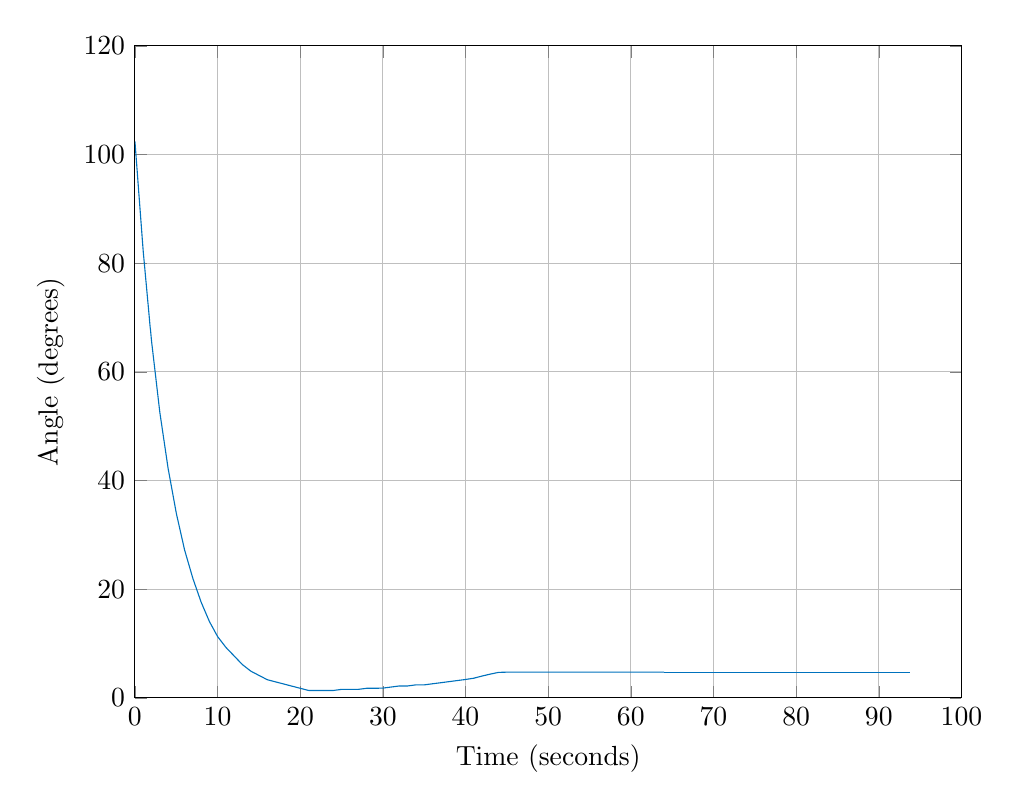
\begin{tikzpicture}

\begin{axis}[%
width=4.133in,
height=3.26in,
at={(0.693in,0.44in)},
scale only axis,
xmin=0,
xmax=100,
xmajorgrids,
xlabel={Time (seconds)},
ymin=0,
ymax=120,
ymajorgrids,
ylabel={Angle (degrees)},
axis background/.style={fill=white}
]
\addplot [color=mycolor1,solid,forget plot]
  table[row sep=crcr]{%
0	102.4204\\
0.0178437059999993	102.2504\\
0.033513767	101.9344\\
0.0486911009999998	101.6224\\
0.0645632799999993	101.3064\\
0.0799840889999997	100.9764\\
0.0959715	100.6624\\
0.112295632999999	100.3424\\
0.128229063999999	100.0224\\
0.143910206999999	99.7004\\
0.159928441	99.3664\\
0.176152943999999	99.0464\\
0.192425278999999	98.7264\\
0.208527363999999	98.4044\\
0.227737754	98.0704\\
0.239854103999999	97.7544\\
0.255899952	97.4344\\
0.274114254	97.1004\\
0.289229026	96.7804\\
0.304297693	96.4584\\
0.319873955999999	96.1364\\
0.338042614999999	95.8044\\
0.353025347999999	95.4924\\
0.368076835999999	95.1604\\
0.383865511	94.8244\\
0.399882251999999	94.5184\\
0.415894704	94.2004\\
0.431895043	93.8644\\
0.448025642999999	93.5424\\
0.463981650999999	93.1744\\
0.480033808	92.8984\\
0.496022775999999	92.5784\\
0.511983003999999	92.2584\\
0.527909216	91.9384\\
0.543889769999999	91.6144\\
0.560055393999999	91.2904\\
0.576215790999999	90.9664\\
0.591955429	90.6404\\
0.60819942	90.3204\\
0.624084398	89.9944\\
0.640243915999999	89.6624\\
0.656047362	89.3404\\
0.672046387	89.0244\\
0.688393293	88.7024\\
0.704219884	88.3764\\
0.720120300999999	88.0544\\
0.735942135	87.7284\\
0.75196465	87.4084\\
0.768030811999999	87.0824\\
0.783912045	86.7624\\
0.800034835999999	86.4384\\
0.816473907	86.1144\\
0.832037347999999	85.7884\\
0.847862807	85.4684\\
0.863909337999999	85.1464\\
0.879818705	84.8204\\
0.895730251	84.4864\\
0.911775856999999	84.1684\\
0.927972553999999	83.8484\\
0.944022214	83.5244\\
0.959966536999999	83.2024\\
0.976029036999999	82.8804\\
0.992000530999999	82.5584\\
1.013210978	82.1624\\
1.025242573	81.9304\\
1.040677109	81.6784\\
1.05613324	81.4244\\
1.072063816	81.1584\\
1.087979324	80.9004\\
1.104047391	80.6284\\
1.120022078	80.3664\\
1.135987059	80.0984\\
1.151992387	79.8344\\
1.167905323	79.5784\\
1.183795134	79.3144\\
1.202062519	79.0384\\
1.217390884	78.7784\\
1.232876261	78.5144\\
1.248291119	78.2404\\
1.264026532	77.9844\\
1.280153379	77.7224\\
1.295896239	77.4464\\
1.311864756	77.1844\\
1.327921734	76.9244\\
1.343763724	76.6644\\
1.359790826	76.3984\\
1.375865917	76.1304\\
1.392015545	75.8584\\
1.408020409	75.5924\\
1.424158791	75.3304\\
1.440044225	75.0684\\
1.456026168	74.8004\\
1.472055903	74.5384\\
1.487963161	74.2764\\
1.504123869	74.0124\\
1.519947884	73.7464\\
1.536116855	73.4784\\
1.552001913	73.2164\\
1.567874993	72.9504\\
1.584081435	72.6864\\
1.600012802	72.4224\\
1.616024903	72.1564\\
1.631993902	71.8904\\
1.648148946	71.6244\\
1.664024227	71.3584\\
1.680070736	71.0944\\
1.696174635	70.8324\\
1.71235635	70.5664\\
1.728021204	70.3004\\
1.744135561	70.0384\\
1.759830059	69.7724\\
1.775899719	69.4444\\
1.791883991	69.1804\\
1.807897225	68.9024\\
1.824024632	68.6384\\
1.839992142	68.3784\\
1.856035874	68.1084\\
1.888329801	67.7904\\
1.904617618	67.5204\\
1.920408043	67.2564\\
1.936312135	66.9964\\
1.952533603	66.7364\\
1.968452503	66.4664\\
1.984599146	66.2064\\
2.000560188	65.9404\\
2.018346505	65.6724\\
2.033564088	65.4444\\
2.048625724	65.2424\\
2.064415153	65.0424\\
2.08040868	64.8224\\
2.096564463	64.6164\\
2.112573873	64.4084\\
2.12852565	64.2024\\
2.144587553	63.9944\\
2.160788052	63.7884\\
2.176489097	63.5764\\
2.192592151	63.3684\\
2.208528185	63.1584\\
2.22446301	62.9484\\
2.240479805	62.7384\\
2.256533141	62.5284\\
2.272546203	62.3204\\
2.28846131	62.1104\\
2.304511362	61.9024\\
2.320505427	61.6904\\
2.336579228	61.4844\\
2.352571358	61.2704\\
2.368808464	61.0604\\
2.384500985	60.8524\\
2.400473536	60.6484\\
2.416501348	60.4384\\
2.432851249	60.2244\\
2.448558679	60.0144\\
2.464923816	59.8064\\
2.480517047	59.5944\\
2.496601326	59.3884\\
2.51506791	59.1704\\
2.530249127	58.9624\\
2.545355271	58.7584\\
2.560976852	58.5544\\
2.5769232	58.3444\\
2.592538158	58.1344\\
2.608512623	57.9264\\
2.624560376	57.7184\\
2.640478253	57.5044\\
2.656520101	57.2944\\
2.672483592	57.0864\\
2.688451547	56.8804\\
2.70454536	56.6584\\
2.720563018	56.4504\\
2.736565094	56.2444\\
2.752542556	56.0384\\
2.76852688	55.8284\\
2.784677941	55.6224\\
2.800534539	55.4144\\
2.81648941	55.2064\\
2.832490807	54.9984\\
2.848487649	54.7884\\
2.864412446	54.5784\\
2.880524053	54.3684\\
2.896539606	54.1564\\
2.912411216	53.9484\\
2.928469504	53.7384\\
2.944483715	53.5284\\
2.960420608	53.3184\\
2.976574613	53.1084\\
2.992515931	52.8984\\
3.010755928	52.6924\\
3.025699354	52.4644\\
3.040766268	52.3184\\
3.056420661	52.1644\\
3.072427746	52.0064\\
3.088511924	51.8344\\
3.104539641	51.6744\\
3.120556101	51.5084\\
3.136519331	51.3384\\
3.152539863	51.1764\\
3.168513325	51.0124\\
3.184464712	50.8504\\
3.20062299	50.6884\\
3.216583033	50.5224\\
3.232488546	50.3564\\
3.248591373	50.1944\\
3.264588189	50.0284\\
3.280476017	49.8644\\
3.2965767	49.6984\\
3.312546234	49.5344\\
3.328566724	49.3684\\
3.344486631	49.2044\\
3.360539419	49.0384\\
3.376509896	48.8724\\
3.392461128	48.7084\\
3.408506755	48.5404\\
3.424462172	48.3784\\
3.440514604	48.2084\\
3.45652196	48.0464\\
3.472506853	47.8804\\
3.488474867	47.7144\\
3.504451049	47.5504\\
3.520446502	47.3904\\
3.536429109	47.2244\\
3.552488935	47.0604\\
3.568511009	46.8944\\
3.584408006	46.7304\\
3.600472127	46.5644\\
3.616610099	46.3924\\
3.632522141	46.2284\\
3.648474939	46.0684\\
3.664536963	45.9044\\
3.680753938	45.7444\\
3.696509728	45.5744\\
3.712483933	45.3864\\
3.728469025	45.2464\\
3.744480848	45.0764\\
3.760519855	44.9144\\
3.776416265	44.7484\\
3.792473527	44.5884\\
3.808607709	44.4164\\
3.824515704	44.2524\\
3.840765699	44.0904\\
3.856641166	43.9244\\
3.872583237	43.7604\\
3.888966093	43.5964\\
3.904540583	43.4244\\
3.92062075	43.2584\\
3.936657044	43.0984\\
3.952688041	42.9324\\
3.96868164	42.7744\\
3.984400611	42.6044\\
4.000423818	42.4404\\
4.018008613	42.2784\\
4.033402543	42.1304\\
4.048739047	42.0004\\
4.064553129	41.8644\\
4.08051862	41.7384\\
4.09649306	41.6084\\
4.112475163	41.4764\\
4.12849002	41.3444\\
4.144448434	41.2084\\
4.160443396	41.0764\\
4.176496009	40.9404\\
4.192373997	40.8104\\
4.208356251	40.6784\\
4.224517001	40.5464\\
4.240614345	40.4084\\
4.256476142	40.2704\\
4.272489845	40.1424\\
4.288462487	40.0084\\
4.304420715	39.8764\\
4.320440619	39.7444\\
4.33647488	39.6084\\
4.352425742	39.4784\\
4.368555529	39.3464\\
4.384515838	39.2124\\
4.400469832	39.0744\\
4.416490349	38.9424\\
4.432451172	38.8104\\
4.448407708	38.6784\\
4.464604917	38.5484\\
4.480751076	38.4104\\
4.496616916	38.2784\\
4.512624521	38.1464\\
4.528780829	38.0164\\
4.544621612	37.8804\\
4.560607337	37.7444\\
4.576610263	37.6124\\
4.592622694	37.4784\\
4.608568069	37.3484\\
4.624524218	37.2144\\
4.640442205	37.0804\\
4.656452046	36.9484\\
4.672635084	36.8144\\
4.688628277	36.6804\\
4.704623384	36.5484\\
4.720522625	36.4164\\
4.736479204	36.2804\\
4.752619225	36.1484\\
4.768592373	36.0164\\
4.78462729	35.8804\\
4.800693349	35.7504\\
4.816625443	35.6164\\
4.832826146	35.4824\\
4.848648652	35.3484\\
4.864599048	35.2164\\
4.880616997	35.0844\\
4.896687265	34.9524\\
4.912534768	34.8164\\
4.928513092	34.6844\\
4.944626397	34.5504\\
4.960495845	34.4184\\
4.976382396	34.2864\\
4.992481153	34.1524\\
5.011154319	34.0124\\
5.026280087	33.8784\\
5.041350769	33.7824\\
5.056569306	33.6804\\
5.072364011	33.5704\\
5.088435806	33.4584\\
5.105135259	33.3464\\
5.120568443	33.2404\\
5.136488079	33.1384\\
5.152440841	33.0304\\
5.168416627	32.9244\\
5.184734592	32.8164\\
5.200437456	32.7124\\
5.216607527	32.6044\\
5.232619463	32.4944\\
5.248655031	32.3864\\
5.264967779	32.2784\\
5.280514687	32.1704\\
5.296460045	32.0624\\
5.312558582	31.9564\\
5.328867759	31.8484\\
5.344574516	31.7404\\
5.360437622	31.6304\\
5.376507811	31.5244\\
5.392449991	31.4184\\
5.408621104	31.3084\\
5.424537598	31.1984\\
5.441775271	31.0924\\
5.457042383	30.9844\\
5.472500048	30.8764\\
5.488466481	30.7684\\
5.504557724	30.6584\\
5.520578947	30.5524\\
5.536533371	30.4464\\
5.552569974	30.3344\\
5.568348402	30.2284\\
5.586790633	30.1184\\
5.602176025	30.0124\\
5.617492972	29.9064\\
5.632748143	29.7964\\
5.64856292	29.6924\\
5.664557883	29.5844\\
5.680594806	29.4764\\
5.696651558	29.3684\\
5.712774654	29.2604\\
5.728468716	29.1544\\
5.744638682	29.0444\\
5.760561548	28.9344\\
5.776474239	28.8284\\
5.792579832	28.7204\\
5.808441445	28.6124\\
5.82450396	28.5084\\
5.840517311	28.3984\\
5.856613822	28.2844\\
5.872530187	28.1784\\
5.888559838	28.0704\\
5.904495004	27.9644\\
5.920534235	27.8584\\
5.936511398	27.7484\\
5.952500844	27.6384\\
5.968551088	27.5304\\
5.984958295	27.4224\\
6.000542365	27.3184\\
6.017901196	27.2164\\
6.03292309	27.1264\\
6.048406363	27.0404\\
6.066602453	26.9504\\
6.081630188	26.8704\\
6.096737458	26.7904\\
6.115192431	26.7024\\
6.128625287	26.6224\\
6.144845759	26.5384\\
6.160460071	26.4544\\
6.176535289	26.3724\\
6.192485612	26.2864\\
6.208509642	26.2024\\
6.224437643	26.1204\\
6.240545548	26.0384\\
6.256525372	25.9544\\
6.272419963	25.8704\\
6.288546796	25.7864\\
6.304865727	25.7024\\
6.320629427	25.6184\\
6.337891659	25.5324\\
6.353167462	25.4504\\
6.368646614	25.3684\\
6.384658866	25.2844\\
6.4005265	25.2004\\
6.416576486	25.1164\\
6.432566883	25.0304\\
6.448535044	24.9484\\
6.464591993	24.8644\\
6.480595423	24.7844\\
6.496611176	24.6964\\
6.512436761	24.6144\\
6.528480893	24.5304\\
6.544501819	24.4484\\
6.560591801	24.3624\\
6.57654681	24.2784\\
6.592460396	24.1964\\
6.608514785	24.1124\\
6.624557251	24.0284\\
6.641652116	23.9424\\
6.656865838	23.8604\\
6.672525207	23.7784\\
6.688389791	23.6924\\
6.704552874	23.6104\\
6.720624229	23.5264\\
6.736571925	23.4424\\
6.752555434	23.3544\\
6.76856402	23.2724\\
6.785379702	23.1884\\
6.800655728	23.1064\\
6.816749564	23.0224\\
6.832553701	22.9384\\
6.848631418	22.8564\\
6.864682266	22.7744\\
6.880494028	22.6884\\
6.896848174	22.6064\\
6.912576945	22.5224\\
6.928595878	22.4364\\
6.944478478	22.3524\\
6.96040604	22.2684\\
6.976501421	22.1844\\
6.992373107	22.1024\\
7.016460852	22.0124\\
7.02509267	21.9264\\
7.040385323	21.8624\\
7.056487801	21.8004\\
7.072438274	21.7284\\
7.090744646	21.6544\\
7.106003617	21.5884\\
7.121221289	21.5164\\
7.136647424	21.4504\\
7.152518375	21.3824\\
7.168594203	21.3124\\
7.184519189	21.2424\\
7.20063109	21.1724\\
7.216551574	21.1024\\
7.232782972	21.0324\\
7.248369051	20.9624\\
7.264649667	20.8944\\
7.280741453	20.8244\\
7.296924823	20.7524\\
7.312696495	20.6844\\
7.328748196	20.6144\\
7.344565703	20.5444\\
7.360554754	20.4744\\
7.376513672	20.4064\\
7.392527533	20.3344\\
7.408615529	20.2604\\
7.424549496	20.1924\\
7.440561604	20.1264\\
7.456509217	20.0564\\
7.472484204	19.9864\\
7.488577937	19.9124\\
7.504418173	19.8444\\
7.520480427	19.7744\\
7.536563579	19.7064\\
7.552588359	19.6364\\
7.5688742	19.5664\\
7.58543245	19.4964\\
7.600747134	19.4264\\
7.616536771	19.3564\\
7.632490626	19.2884\\
7.648559333	19.2164\\
7.664625913	19.1504\\
7.680594352	19.0804\\
7.696510688	19.0104\\
7.712400703	18.9384\\
7.728602764	18.8724\\
7.74456861	18.8004\\
7.760396395	18.7304\\
7.776488296	18.6584\\
7.792515289	18.5904\\
7.80868876	18.5204\\
7.824601902	18.4504\\
7.840474128	18.3804\\
7.85652512	18.3124\\
7.87259662	18.2424\\
7.888531305	18.1724\\
7.904428213	18.1024\\
7.9205942	18.0344\\
7.936616323	17.9644\\
7.952530923	17.8944\\
7.968398313	17.8224\\
7.984497892	17.7524\\
8.000479693	17.6824\\
8.018088414	17.6124\\
8.033106332	17.5504\\
8.04841312	17.4944\\
8.064427889	17.4384\\
8.082695867	17.3804\\
8.098011892	17.3264\\
8.113527197	17.2684\\
8.128672415	17.2084\\
8.146038278	17.1544\\
8.16119108	17.0984\\
8.176410305	17.0404\\
8.19262314	16.9844\\
8.208521473	16.9284\\
8.224560112	16.8704\\
8.240487502	16.8124\\
8.256436659	16.7564\\
8.27243641	16.7004\\
8.2884056	16.6424\\
8.304773541	16.5824\\
8.32076603	16.5304\\
8.336810792	16.4684\\
8.353550747	16.4104\\
8.368821024	16.3564\\
8.384782076	16.2984\\
8.40062861	16.2404\\
8.416573488	16.1844\\
8.43265872	16.1284\\
8.448572792	16.0704\\
8.464637009	16.0144\\
8.480537135	15.9564\\
8.49697059	15.9004\\
8.512780748	15.8404\\
8.528758684	15.7864\\
8.544693001	15.7304\\
8.560442722	15.6704\\
8.576475142	15.6144\\
8.592543156	15.5584\\
8.608581569	15.5004\\
8.624494069	15.4424\\
8.640565785	15.3864\\
8.656583188	15.3304\\
8.67247246	15.2724\\
8.688418354	15.2124\\
8.70440397	15.1564\\
8.720407351	15.0984\\
8.736563163	15.0424\\
8.752565035	14.9884\\
8.768531838	14.9284\\
8.784510273	14.8724\\
8.80055832	14.8144\\
8.816544648	14.7544\\
8.83250093	14.7004\\
8.848550275	14.6424\\
8.864545048	14.5884\\
8.880463795	14.5304\\
8.896591909	14.4724\\
8.91274107	14.4184\\
8.928686683	14.3604\\
8.944981502	14.3004\\
8.960561903	14.2404\\
8.976484876	14.1864\\
8.992481161	14.1304\\
9.014354188	14.0704\\
9.02647968	14.0144\\
9.041469344	13.9744\\
9.056645342	13.9324\\
9.072467122	13.8844\\
9.088498047	13.8404\\
9.104891983	13.7984\\
9.121109076	13.7544\\
9.137346593	13.7104\\
9.152654082	13.6664\\
9.168404319	13.6204\\
9.184489202	13.5764\\
9.200505816	13.5324\\
9.216553258	13.4884\\
9.232549241	13.4464\\
9.248502954	13.4004\\
9.264498779	13.3564\\
9.280627804	13.3104\\
9.296613545	13.2664\\
9.312446655	13.2224\\
9.328723405	13.1764\\
9.344769016	13.1344\\
9.360688991	13.0884\\
9.376810769	13.0464\\
9.392493535	12.9984\\
9.4084725	12.9564\\
9.424726916	12.9104\\
9.440555644	12.8664\\
9.456470687	12.8224\\
9.472564277	12.7764\\
9.488464524	12.7344\\
9.504413782	12.6884\\
9.520617656	12.6464\\
9.53647959	12.6004\\
9.552450317	12.5564\\
9.568544041	12.5124\\
9.584549431	12.4664\\
9.600548678	12.4224\\
9.616544151	12.3764\\
9.632739127	12.3344\\
9.648575063	12.2904\\
9.664658996	12.2464\\
9.680605849	12.1884\\
9.696453782	12.1444\\
9.712501478	12.1004\\
9.728864913	12.0544\\
9.744804543	12.0104\\
9.760508449	11.9684\\
9.776451816	11.9244\\
9.792665807	11.8784\\
9.808480239	11.8344\\
9.824567047	11.7904\\
9.840502115	11.7444\\
9.85647454	11.7004\\
9.872532654	11.6544\\
9.888743515	11.6144\\
9.904396428	11.5684\\
9.920526941	11.5224\\
9.936488548	11.4784\\
9.952354623	11.4344\\
9.968401114	11.3904\\
9.984574448	11.3444\\
10.000520059	11.3004\\
10.017958712	11.2604\\
10.032908314	11.2224\\
10.048417911	11.1924\\
10.06442105	11.1604\\
10.080455208	11.1284\\
10.096438917	11.0984\\
10.112540239	11.0684\\
10.128696354	11.0344\\
10.144812055	11.0024\\
10.16056236	10.9704\\
10.176877033	10.9404\\
10.192740899	10.9104\\
10.208374472	10.8744\\
10.224432361	10.8424\\
10.240581533	10.8124\\
10.25650467	10.7784\\
10.272569275	10.7484\\
10.288495391	10.7184\\
10.304677805	10.6844\\
10.320526736	10.6524\\
10.336434248	10.6224\\
10.352748917	10.5904\\
10.368428961	10.5604\\
10.384480653	10.5284\\
10.400471025	10.4944\\
10.416575352	10.4624\\
10.432540847	10.4324\\
10.448574932	10.4004\\
10.464661653	10.3704\\
10.480530328	10.3384\\
10.496523774	10.3044\\
10.512598809	10.2724\\
10.528473695	10.2424\\
10.544829804	10.2104\\
10.560851172	10.1804\\
10.576423676	10.1484\\
10.593162208	10.1144\\
10.608574746	10.0824\\
10.624438603	10.0524\\
10.640401014	10.0184\\
10.656558065	9.98839999999998\\
10.672570034	9.95439999999999\\
10.688475891	9.92439999999999\\
10.70454135	9.89239999999998\\
10.720454747	9.86239999999999\\
10.736555304	9.8304\\
10.752621066	9.8004\\
10.768369478	9.76639999999999\\
10.784558656	9.73439999999999\\
10.800597267	9.7024\\
10.816549307	9.6704\\
10.832556016	9.64039999999999\\
10.848645818	9.60839999999999\\
10.864542965	9.57640000000001\\
10.880576108	9.5444\\
10.896664475	9.51239999999999\\
10.912554524	9.4804\\
10.928512098	9.4504\\
10.944600707	9.4204\\
10.960821992	9.38639999999999\\
10.976551429	9.35239999999999\\
10.992542716	9.3224\\
11.011579313	9.29040000000001\\
11.026776332	9.26239999999999\\
11.041793186	9.23639999999999\\
11.056815431	9.21439999999998\\
11.072425641	9.18640000000001\\
11.088460128	9.16240000000001\\
11.10456324	9.13639999999999\\
11.120441841	9.1104\\
11.136525816	9.0864\\
11.152482888	9.06039999999999\\
11.168544584	9.03440000000001\\
11.184466619	9.01039999999999\\
11.200594696	8.98439999999999\\
11.216474092	8.9584\\
11.232571332	8.93640000000001\\
11.248641051	8.90639999999999\\
11.264485212	8.88239999999999\\
11.280493872	8.85639999999998\\
11.296656837	8.8304\\
11.31269187	8.80639999999998\\
11.328590059	8.78039999999999\\
11.344812531	8.7564\\
11.360853221	8.7304\\
11.376480851	8.7064\\
11.392601412	8.68039999999999\\
11.408679362	8.65639999999999\\
11.425300651	8.6284\\
11.440942769	8.60439999999998\\
11.456373444	8.57640000000001\\
11.47235479	8.55439999999999\\
11.488670237	8.5264\\
11.504526005	8.50039999999998\\
11.520539376	8.47639999999998\\
11.536555829	8.4504\\
11.55256538	8.42639999999999\\
11.568536572	8.40039999999999\\
11.584586013	8.3764\\
11.600576064	8.35039999999999\\
11.616733918	8.32640000000001\\
11.633159468	8.29839999999999\\
11.648648032	8.2764\\
11.664672206	8.24639999999998\\
11.680528417	8.22639999999998\\
11.696668669	8.19640000000001\\
11.712800789	8.17439999999999\\
11.728766144	8.1464\\
11.744731658	8.12039999999999\\
11.760749741	8.09639999999999\\
11.776543314	8.07040000000001\\
11.792594178	8.04639999999999\\
11.808531135	8.02039999999998\\
11.824460534	7.99639999999998\\
11.84041236	7.9704\\
11.856478101	7.94640000000001\\
11.872552308	7.9204\\
11.888431781	7.8964\\
11.904474007	7.86839999999999\\
11.920477278	7.84439999999999\\
11.936586654	7.81640000000002\\
11.95247765	7.7924\\
11.968472612	7.76639999999999\\
11.984539466	7.74039999999999\\
12.000456869	7.71639999999999\\
12.017836211	7.6884\\
12.032860443	7.6644\\
12.048419787	7.63839999999999\\
12.064416151	7.61639999999998\\
12.080441471	7.58839999999999\\
12.096552536	7.56640000000002\\
12.112987269	7.5364\\
12.12843004	7.51639999999999\\
12.144516149	7.48639999999999\\
12.160616359	7.46039999999999\\
12.176557369	7.4344\\
12.192440223	7.41240000000001\\
12.208900488	7.38639999999999\\
12.224596528	7.3604\\
12.242410633	7.3364\\
12.257778539	7.30839999999998\\
12.273025336	7.2864\\
12.288634553	7.26039999999999\\
12.304465709	7.23639999999999\\
12.320530137	7.2084\\
12.336632042	7.18640000000001\\
12.352565715	7.15639999999999\\
12.368573125	7.13239999999999\\
12.384582234	7.10639999999998\\
12.400515224	7.0804\\
12.416675513	7.05639999999998\\
12.432559693	7.03039999999999\\
12.448591684	7.0064\\
12.46458587	6.9804\\
12.480685587	6.9564\\
12.496538914	6.93039999999999\\
12.512649715	6.90639999999999\\
12.528816601	6.88039999999999\\
12.544594896	6.85639999999998\\
12.560375477	6.82640000000001\\
12.576670286	6.80439999999999\\
12.592552825	6.7764\\
12.608447716	6.75239999999999\\
12.624584671	6.72639999999998\\
12.640664292	6.7004\\
12.656638059	6.67639999999999\\
12.67235935	6.65039999999999\\
12.688736102	6.6264\\
12.70450626	6.60039999999999\\
12.720654301	6.57640000000001\\
12.736732431	6.54639999999999\\
12.752466603	6.5264\\
12.768536101	6.49639999999998\\
12.784800343	6.47239999999999\\
12.800544888	6.44640000000001\\
12.816635752	6.4204\\
12.832451024	6.3964\\
12.848581431	6.37039999999999\\
12.864499343	6.34639999999999\\
12.880848615	6.32040000000001\\
12.896489588	6.29639999999999\\
12.915082934	6.26839999999999\\
12.93088134	6.24639999999998\\
12.947101012	6.21639999999999\\
12.962445522	6.19640000000001\\
12.97836381	6.1664\\
12.993700277	6.1464\\
13.011305348	6.11639999999998\\
13.024477807	6.09439999999998\\
13.04051089	6.07640000000001\\
13.056500128	6.05839999999999\\
13.073569302	6.04040000000001\\
13.088723694	6.0204\\
13.104541545	6.00239999999999\\
13.120336826	5.98239999999998\\
13.136555473	5.96239999999999\\
13.152559746	5.94240000000001\\
13.168566735	5.9264\\
13.184531729	5.90639999999999\\
13.200568741	5.8884\\
13.216508764	5.87039999999999\\
13.232621829	5.85039999999999\\
13.248742442	5.8304\\
13.264639435	5.8124\\
13.280820791	5.7924\\
13.296539521	5.77239999999999\\
13.312799869	5.7544\\
13.328821576	5.73439999999999\\
13.344527382	5.71639999999999\\
13.36045183	5.69840000000001\\
13.376596206	5.68039999999999\\
13.392410531	5.6604\\
13.408424737	5.6404\\
13.42447648	5.6224\\
13.440531209	5.60239999999999\\
13.456450185	5.58239999999999\\
13.472529807	5.5624\\
13.49007211	5.5424\\
13.506341043	5.52439999999999\\
13.521511373	5.5044\\
13.537018377	5.48839999999998\\
13.552566997	5.47039999999998\\
13.568534106	5.4504\\
13.584602539	5.43039999999999\\
13.600625839	5.41239999999999\\
13.616937082	5.39239999999999\\
13.632542223	5.3724\\
13.648397288	5.35439999999998\\
13.664539188	5.3364\\
13.680740049	5.3164\\
13.696418772	5.29839999999999\\
13.714888533	5.2764\\
13.730200137	5.26039999999999\\
13.745493776	5.24039999999999\\
13.76073449	5.22239999999999\\
13.776631164	5.2024\\
13.792515963	5.1824\\
13.80852026	5.1644\\
13.824581382	5.14439999999999\\
13.840461901	5.12639999999999\\
13.856555436	5.10839999999999\\
13.872466568	5.08839999999999\\
13.888398425	5.07039999999999\\
13.904550675	5.0504\\
13.920579258	5.0324\\
13.936591582	5.01239999999999\\
13.952543038	4.99239999999999\\
13.968578627	4.97439999999999\\
13.984508772	4.95439999999999\\
14.000754088	4.93639999999999\\
14.018348637	4.9204\\
14.032443328	4.90439999999998\\
14.048447351	4.8904\\
14.064520545	4.88039999999999\\
14.080523	4.86839999999999\\
14.096430535	4.85439999999998\\
14.112490016	4.84039999999999\\
14.1309698	4.8304\\
14.146213625	4.8184\\
14.161473916	4.8004\\
14.176645137	4.79040000000001\\
14.192551746	4.7804\\
14.20836354	4.76439999999999\\
14.224528559	4.7504\\
14.240384452	4.74039999999999\\
14.25652198	4.72839999999999\\
14.272980341	4.71439999999998\\
14.288677217	4.7004\\
14.3045488	4.6904\\
14.320598507	4.68039999999999\\
14.336511853	4.66239999999999\\
14.352553085	4.65039999999999\\
14.368563757	4.6404\\
14.385281759	4.62440000000001\\
14.400644728	4.61039999999998\\
14.416610402	4.60039999999999\\
14.432516029	4.59039999999999\\
14.448550279	4.5744\\
14.464643386	4.5604\\
14.480394149	4.5504\\
14.496490474	4.54040000000001\\
14.512615671	4.52439999999999\\
14.528663603	4.51039999999999\\
14.544565191	4.5004\\
14.562985172	4.48839999999998\\
14.578482168	4.47039999999998\\
14.593694656	4.46039999999999\\
14.609115206	4.4504\\
14.624596642	4.4344\\
14.640483393	4.4204\\
14.656464644	4.4104\\
14.672465027	4.3964\\
14.688626373	4.3844\\
14.704575696	4.36839999999999\\
14.720580836	4.36039999999998\\
14.736589294	4.35039999999999\\
14.75241854	4.33439999999999\\
14.770977569	4.32039999999999\\
14.786224036	4.3104\\
14.801588824	4.2944\\
14.816881431	4.2804\\
14.8328178	4.2704\\
14.848682604	4.26039999999999\\
14.864784278	4.2424\\
14.880789043	4.23039999999999\\
14.896443434	4.22039999999998\\
14.912481906	4.2084\\
14.930935081	4.19239999999999\\
14.946169254	4.18039999999999\\
14.961531081	4.1704\\
14.976558422	4.1604\\
14.992555218	4.14239999999999\\
15.014348444	4.13039999999999\\
15.024579733	4.11839999999999\\
15.040531914	4.10239999999999\\
15.056517037	4.09039999999999\\
15.072386574	4.0804\\
15.088339549	4.07039999999999\\
15.104453975	4.05439999999999\\
15.120509355	4.04040000000001\\
15.136537258	4.0304\\
15.152580392	4.0204\\
15.16863334	4.0044\\
15.184679939	3.99039999999999\\
15.200922662	3.98039999999999\\
15.216588454	3.96639999999999\\
15.23250316	3.9524\\
15.248616293	3.9404\\
15.264680688	3.93039999999999\\
15.280527585	3.91439999999999\\
15.29656196	3.90039999999999\\
15.312592272	3.8904\\
15.328767749	3.88039999999999\\
15.344877871	3.8644\\
15.360806463	3.85039999999999\\
15.37661803	3.84039999999999\\
15.392693529	3.8304\\
15.408538917	3.81440000000001\\
15.424457587	3.8004\\
15.440695198	3.79040000000001\\
15.456622902	3.77439999999999\\
15.472494114	3.76239999999999\\
15.488400475	3.7504\\
15.504557512	3.73839999999998\\
15.520647488	3.72439999999999\\
15.536601213	3.71039999999999\\
15.552509874	3.7004\\
15.568582645	3.6904\\
15.584637458	3.67439999999999\\
15.600507348	3.6604\\
15.616428002	3.65039999999999\\
15.632498294	3.6384\\
15.648497883	3.6224\\
15.664557548	3.61039999999998\\
15.680921342	3.60039999999999\\
15.696535957	3.58439999999999\\
15.712505991	3.57039999999999\\
15.728525386	3.5604\\
15.744454965	3.5504\\
15.760726996	3.53439999999999\\
15.776568818	3.5204\\
15.793030649	3.51039999999999\\
15.808502241	3.5004\\
15.82447187	3.48239999999998\\
15.841666431	3.47039999999998\\
15.857552812	3.46039999999999\\
15.872782017	3.4444\\
15.888418767	3.43039999999999\\
15.904413312	3.4204\\
15.920424973	3.4104\\
15.936534323	3.39439999999999\\
15.952563152	3.38039999999999\\
15.968377395	3.37039999999999\\
15.984531173	3.36039999999998\\
16.000490181	3.34439999999998\\
16.018504782	3.33239999999999\\
16.033901965	3.32640000000001\\
16.049229713	3.3164\\
16.064527555	3.3164\\
16.080785248	3.30639999999998\\
16.09675905	3.30239999999999\\
16.112508796	3.29639999999999\\
16.12868132	3.28639999999999\\
16.144594458	3.28439999999999\\
16.160794962	3.2764\\
16.176568963	3.2684\\
16.192465792	3.26439999999999\\
16.208734489	3.2564\\
16.224524703	3.2504\\
16.240646412	3.24640000000001\\
16.256553905	3.23639999999997\\
16.272537037	3.23239999999998\\
16.288460579	3.22639999999998\\
16.304531826	3.21639999999999\\
16.320642029	3.21439999999998\\
16.336832646	3.2064\\
16.352728697	3.19840000000001\\
16.368534809	3.1944\\
16.384382577	3.18639999999999\\
16.400573336	3.1824\\
16.416379053	3.17639999999999\\
16.4325989	3.16639999999998\\
16.448803442	3.16239999999999\\
16.46444752	3.15639999999999\\
16.480503779	3.1464\\
16.496403361	3.14439999999999\\
16.512489494	3.13640000000001\\
16.528435836	3.1284\\
16.544481162	3.12440000000001\\
16.560508522	3.1164\\
16.576508861	3.11240000000001\\
16.592474216	3.10639999999998\\
16.608518726	3.09639999999999\\
16.624486912	3.09239999999998\\
16.640699121	3.0864\\
16.656627387	3.07640000000001\\
16.672588482	3.0744\\
16.688815946	3.0664\\
16.704446758	3.05839999999999\\
16.720700627	3.05639999999998\\
16.736617136	3.04639999999999\\
16.752488128	3.0424\\
16.768742306	3.03639999999999\\
16.784454782	3.0264\\
16.800558526	3.02239999999999\\
16.81652114	3.0164\\
16.832538834	3.0064\\
16.848552167	3.0044\\
16.864442079	2.99640000000001\\
16.880467175	2.99039999999999\\
16.896464289	2.98639999999997\\
16.912694819	2.97639999999998\\
16.929031107	2.97239999999999\\
16.945051996	2.96639999999999\\
16.960967342	2.9564\\
16.976475706	2.95439999999999\\
16.992359732	2.94640000000001\\
17.010607996	2.93839999999999\\
17.0258298	2.9344\\
17.04120617	2.92639999999999\\
17.056779742	2.91839999999999\\
17.073768249	2.91639999999998\\
17.088895987	2.90639999999999\\
17.105535766	2.90239999999999\\
17.120901873	2.8964\\
17.136560723	2.88640000000001\\
17.154979709	2.8844\\
17.170337857	2.8764\\
17.18600013	2.86839999999999\\
17.201344312	2.8664\\
17.216886984	2.85639999999998\\
17.232754768	2.85239999999999\\
17.24855249	2.84639999999999\\
17.264556035	2.8364\\
17.280447084	2.83239999999999\\
17.296784789	2.82640000000001\\
17.312603937	2.8164\\
17.331734367	2.81440000000001\\
17.344528559	2.80639999999998\\
17.360471786	2.79639999999999\\
17.376485368	2.79639999999999\\
17.392507377	2.78639999999999\\
17.408530344	2.7824\\
17.424440312	2.7764\\
17.440447495	2.7664\\
17.456424546	2.76239999999999\\
17.47258031	2.7564\\
17.488482174	2.74640000000001\\
17.507013755	2.74440000000001\\
17.522303212	2.73639999999997\\
17.537595818	2.72839999999999\\
17.552889875	2.72639999999998\\
17.568564257	2.71639999999999\\
17.58455727	2.71239999999999\\
17.600612799	2.7064\\
17.616431657	2.69640000000001\\
17.632427984	2.6944\\
17.648666823	2.68639999999999\\
17.664540847	2.6784\\
17.683213676	2.67439999999999\\
17.698473126	2.66639999999998\\
17.713748644	2.6604\\
17.729293819	2.65639999999999\\
17.744383906	2.6464\\
17.762881059	2.64239999999999\\
17.778291468	2.63640000000001\\
17.793582416	2.6264\\
17.808840858	2.62440000000001\\
17.824933003	2.6164\\
17.840580405	2.60839999999999\\
17.856489446	2.60439999999998\\
17.872576988	2.59639999999999\\
17.888423862	2.59239999999998\\
17.904566459	2.5864\\
17.920363355	2.57640000000001\\
17.93654417	2.57239999999999\\
17.952520805	2.5664\\
17.968619868	2.55639999999998\\
17.984391741	2.55439999999999\\
18.000743997	2.54639999999999\\
18.018082901	2.5384\\
18.033282286	2.53439999999999\\
18.048605366	2.5264\\
18.0646471	2.52239999999999\\
18.080524891	2.5164\\
18.096464318	2.5064\\
18.112987533	2.50239999999999\\
18.130169491	2.49640000000001\\
18.14539017	2.48639999999997\\
18.16060711	2.48439999999998\\
18.176572787	2.47639999999998\\
18.192539914	2.46839999999999\\
18.208432258	2.46639999999999\\
18.224654688	2.4564\\
18.240463792	2.4524\\
18.256442948	2.44640000000001\\
18.272366587	2.43639999999999\\
18.288362593	2.4324\\
18.304538575	2.42639999999999\\
18.320412741	2.41639999999998\\
18.336568124	2.41439999999999\\
18.352768772	2.40639999999999\\
18.368553362	2.40239999999999\\
18.384636663	2.3964\\
18.40056329	2.38640000000001\\
18.416648443	2.38239999999999\\
18.4326125	2.3764\\
18.448578623	2.3664\\
18.464567223	2.3644\\
18.480495386	2.35639999999998\\
18.496940547	2.3484\\
18.514438505	2.34639999999999\\
18.52988946	2.3364\\
18.545135328	2.3284\\
18.560588963	2.32640000000001\\
18.576931593	2.3164\\
18.594404497	2.3124\\
18.609765687	2.30639999999998\\
18.625070865	2.29639999999999\\
18.640875412	2.2944\\
18.656455146	2.28639999999999\\
18.672544326	2.27839999999999\\
18.688585969	2.2764\\
18.704466236	2.2664\\
18.720518613	2.26039999999999\\
18.736564255	2.2564\\
18.752539592	2.24640000000001\\
18.768579937	2.2424\\
18.784608769	2.23639999999997\\
18.800559717	2.22639999999998\\
18.819111448	2.22439999999999\\
18.834378006	2.21639999999999\\
18.849624978	2.2084\\
18.864782867	2.2064\\
18.88059725	2.19640000000001\\
18.896482624	2.19239999999999\\
18.912480121	2.18639999999999\\
18.928486444	2.17639999999999\\
18.944585462	2.17439999999999\\
18.960530853	2.16639999999998\\
18.976475525	2.15839999999999\\
18.992516569	2.15439999999998\\
19.014230916	2.1464\\
19.026288514	2.13640000000001\\
19.041652555	2.13640000000001\\
19.057410077	2.1264\\
19.07435733	2.1224\\
19.08954413	2.1164\\
19.106254601	2.10639999999998\\
19.121448911	2.10439999999998\\
19.136766774	2.09639999999999\\
19.152484766	2.08839999999999\\
19.168509462	2.0864\\
19.184590925	2.07640000000001\\
19.200587603	2.07239999999999\\
19.216535618	2.0664\\
19.232596218	2.05639999999998\\
19.248592214	2.05239999999999\\
19.26453931	2.04639999999999\\
19.280464185	2.03639999999999\\
19.296471683	2.03439999999999\\
19.31259426	2.0264\\
19.328609714	2.0184\\
19.344778048	2.0164\\
19.361122141	2.0064\\
19.376526304	2.00239999999999\\
19.392628426	1.99640000000001\\
19.410331057	1.98639999999997\\
19.425533153	1.98439999999998\\
19.440755569	1.97639999999998\\
19.456488753	1.96639999999999\\
19.472575822	1.96439999999998\\
19.489148739	1.9564\\
19.50443441	1.94840000000001\\
19.520534423	1.94640000000001\\
19.536465048	1.93639999999999\\
19.552570579	1.9324\\
19.568595111	1.92639999999999\\
19.584548679	1.91639999999998\\
19.600546317	1.91239999999999\\
19.616494226	1.90639999999999\\
19.632455331	1.8984\\
19.648462966	1.89439999999999\\
19.664369554	1.88640000000001\\
19.680650931	1.88239999999999\\
19.696667187	1.8764\\
19.712686459	1.8664\\
19.728942169	1.86240000000001\\
19.744672691	1.85639999999998\\
19.760446522	1.84639999999999\\
19.776567454	1.84439999999998\\
19.792344779	1.8364\\
19.808561307	1.82640000000001\\
19.824491805	1.8244\\
19.841264179	1.8164\\
19.85649045	1.81039999999999\\
19.872621861	1.80639999999998\\
19.888768121	1.79639999999999\\
19.904392825	1.7924\\
19.920828149	1.78639999999999\\
19.936456546	1.7764\\
19.952539877	1.77439999999999\\
19.968564552	1.7664\\
19.984469494	1.75839999999999\\
20.000541707	1.7564\\
20.018468948	1.74640000000001\\
20.033738258	1.74039999999999\\
20.049219963	1.73639999999997\\
20.064662225	1.72639999999998\\
20.081029584	1.72239999999999\\
20.096505386	1.71639999999999\\
20.112473424	1.7064\\
20.128642168	1.70439999999999\\
20.145400267	1.69640000000001\\
20.161610921	1.68839999999999\\
20.176939125	1.68639999999999\\
20.193023004	1.67639999999999\\
20.208646373	1.6724\\
20.224470237	1.66639999999998\\
20.240522103	1.65639999999999\\
20.256393896	1.65239999999999\\
20.272512573	1.6464\\
20.288471321	1.63640000000001\\
20.304565094	1.63640000000001\\
20.320491038	1.6264\\
20.336601669	1.62039999999999\\
20.352549142	1.6164\\
20.36970215	1.60639999999998\\
20.385333493	1.60239999999999\\
20.400723756	1.59639999999999\\
20.416448547	1.5864\\
20.432591652	1.58439999999999\\
20.448514675	1.57640000000001\\
20.464553336	1.5684\\
20.480546309	1.5664\\
20.496582289	1.55639999999998\\
20.512753971	1.55239999999999\\
20.52907392	1.54639999999999\\
20.544653309	1.53639999999999\\
20.560797686	1.5324\\
20.576588261	1.5264\\
20.592421149	1.5164\\
20.608441117	1.51439999999999\\
20.62458857	1.5064\\
20.64053404	1.4984\\
20.658166353	1.49640000000001\\
20.673417503	1.48639999999997\\
20.688760429	1.48039999999999\\
20.704348723	1.47639999999998\\
20.720485427	1.46639999999999\\
20.736542607	1.46239999999999\\
20.752590463	1.4564\\
20.768630561	1.44640000000001\\
20.784830107	1.4444\\
20.800420853	1.43639999999999\\
20.816565919	1.43039999999999\\
20.832670289	1.42639999999999\\
20.848357061	1.41639999999998\\
20.864612128	1.41239999999999\\
20.880835581	1.40639999999999\\
20.896555145	1.3964\\
20.912603577	1.39439999999999\\
20.928478855	1.38640000000001\\
20.944592186	1.3764\\
20.960650636	1.37440000000001\\
20.976597014	1.3664\\
20.992571399	1.3604\\
21.014524074	1.35639999999998\\
21.026493087	1.35239999999999\\
21.041915405	1.35239999999999\\
21.057498441	1.35239999999999\\
21.072747636	1.35239999999999\\
21.088609489	1.35239999999999\\
21.104657799	1.35239999999999\\
21.120812022	1.35239999999999\\
21.136492282	1.35239999999999\\
21.152454962	1.35239999999999\\
21.168513831	1.35239999999999\\
21.18453639	1.35239999999999\\
21.200567369	1.35239999999999\\
21.216437492	1.35239999999999\\
21.232532596	1.35239999999999\\
21.248577227	1.35239999999999\\
21.264610876	1.35239999999999\\
21.280544372	1.35239999999999\\
21.296834514	1.35239999999999\\
21.312544842	1.35239999999999\\
21.328702496	1.35239999999999\\
21.344535859	1.35239999999999\\
21.360558318	1.35239999999999\\
21.376626092	1.35239999999999\\
21.392469903	1.35239999999999\\
21.410379586	1.35239999999999\\
21.425623369	1.35239999999999\\
21.440979575	1.35239999999999\\
21.456573182	1.35239999999999\\
21.472450742	1.35239999999999\\
21.488462361	1.35239999999999\\
21.50462309	1.35239999999999\\
21.520542591	1.35239999999999\\
21.53642373	1.35239999999999\\
21.552581516	1.35239999999999\\
21.568554564	1.35239999999999\\
21.584600661	1.35239999999999\\
21.600543224	1.35239999999999\\
21.616571782	1.35239999999999\\
21.632499556	1.35239999999999\\
21.648475075	1.35239999999999\\
21.664370752	1.35239999999999\\
21.68053814	1.35239999999999\\
21.69648016	1.35239999999999\\
21.712578579	1.35239999999999\\
21.72853377	1.35239999999999\\
21.744609134	1.35239999999999\\
21.761352498	1.35239999999999\\
21.77674326	1.35239999999999\\
21.792502882	1.35239999999999\\
21.80855849	1.35239999999999\\
21.825365307	1.35239999999999\\
21.840633375	1.35239999999999\\
21.856624022	1.35239999999999\\
21.872515151	1.35239999999999\\
21.888564206	1.35239999999999\\
21.904562342	1.35239999999999\\
21.920722343	1.35239999999999\\
21.936503997	1.35239999999999\\
21.952551862	1.35239999999999\\
21.96852453	1.35239999999999\\
21.984631235	1.35239999999999\\
22.000454573	1.35239999999999\\
22.017879311	1.35239999999999\\
22.033071525	1.35239999999999\\
22.048377923	1.35239999999999\\
22.064618353	1.35239999999999\\
22.080412242	1.35239999999999\\
22.096492545	1.35239999999999\\
22.112485263	1.35239999999999\\
22.128526395	1.35239999999999\\
22.144839902	1.35239999999999\\
22.160556802	1.35239999999999\\
22.176490279	1.35239999999999\\
22.192520322	1.35239999999999\\
22.208417566	1.35239999999999\\
22.224443838	1.35239999999999\\
22.240904596	1.35239999999999\\
22.256588245	1.35239999999999\\
22.272532858	1.35239999999999\\
22.288467044	1.35239999999999\\
22.304533076	1.35239999999999\\
22.320507359	1.35239999999999\\
22.336470662	1.35239999999999\\
22.352484302	1.35239999999999\\
22.368525196	1.35239999999999\\
22.384531691	1.35239999999999\\
22.400431321	1.35239999999999\\
22.416531166	1.35239999999999\\
22.432445154	1.35239999999999\\
22.448583004	1.35239999999999\\
22.464503293	1.35239999999999\\
22.480608082	1.35239999999999\\
22.498361423	1.35239999999999\\
22.5135976	1.35239999999999\\
22.529048832	1.35239999999999\\
22.544520982	1.35239999999999\\
22.560526114	1.35239999999999\\
22.576761606	1.35239999999999\\
22.592524616	1.35239999999999\\
22.608594494	1.35239999999999\\
22.624455866	1.35239999999999\\
22.640525444	1.35239999999999\\
22.656628192	1.35239999999999\\
22.672543589	1.35239999999999\\
22.688654077	1.35239999999999\\
22.704532195	1.35239999999999\\
22.720592597	1.35239999999999\\
22.736576185	1.35239999999999\\
22.752585199	1.35239999999999\\
22.768624493	1.35239999999999\\
22.784588383	1.35239999999999\\
22.800483199	1.35239999999999\\
22.816896709	1.35239999999999\\
22.832414114	1.35239999999999\\
22.848619828	1.35239999999999\\
22.864655793	1.35239999999999\\
22.880549806	1.35239999999999\\
22.896779474	1.35239999999999\\
22.912575491	1.35239999999999\\
22.928490723	1.35239999999999\\
22.944747887	1.35239999999999\\
22.960443966	1.35239999999999\\
22.976449843	1.35239999999999\\
22.992529198	1.35239999999999\\
23.013607337	1.35239999999999\\
23.025529339	1.35239999999999\\
23.041205626	1.35239999999999\\
23.056497959	1.35239999999999\\
23.072381468	1.35239999999999\\
23.088570016	1.35239999999999\\
23.104482342	1.35239999999999\\
23.120631926	1.35239999999999\\
23.136661182	1.35239999999999\\
23.152476786	1.35239999999999\\
23.168645054	1.35239999999999\\
23.18440508	1.35239999999999\\
23.200427496	1.35239999999999\\
23.216588585	1.35239999999999\\
23.232605597	1.35239999999999\\
23.248533572	1.35239999999999\\
23.264600617	1.35239999999999\\
23.280423612	1.35239999999999\\
23.296685256	1.35239999999999\\
23.312565541	1.35239999999999\\
23.328628103	1.35239999999999\\
23.344758967	1.35239999999999\\
23.360460696	1.35239999999999\\
23.379036156	1.35239999999999\\
23.392582503	1.35239999999999\\
23.408441011	1.35239999999999\\
23.424533382	1.35239999999999\\
23.440528838	1.35239999999999\\
23.456407785	1.35239999999999\\
23.472505411	1.35239999999999\\
23.488456923	1.35239999999999\\
23.504543879	1.35239999999999\\
23.520574111	1.35239999999999\\
23.536524272	1.35239999999999\\
23.552519367	1.35239999999999\\
23.568572574	1.35239999999999\\
23.584536089	1.35239999999999\\
23.600497104	1.35239999999999\\
23.616587041	1.35239999999999\\
23.632822578	1.35239999999999\\
23.648603953	1.35239999999999\\
23.664529599	1.35239999999999\\
23.680529558	1.35239999999999\\
23.696559064	1.35239999999999\\
23.712667707	1.35239999999999\\
23.728506783	1.35239999999999\\
23.747036445	1.35239999999999\\
23.762346374	1.35239999999999\\
23.777617245	1.35239999999999\\
23.792877236	1.35239999999999\\
23.808506826	1.35239999999999\\
23.824604454	1.35239999999999\\
23.840507522	1.35239999999999\\
23.856481932	1.35239999999999\\
23.872421674	1.35239999999999\\
23.888404701	1.35239999999999\\
23.904583158	1.35239999999999\\
23.920540186	1.35239999999999\\
23.936455874	1.35239999999999\\
23.952670632	1.35239999999999\\
23.968899661	1.35239999999999\\
23.984544074	1.35239999999999\\
24.000493164	1.35239999999999\\
24.016364327	1.35239999999999\\
24.032579577	1.35640000000001\\
24.048542685	1.36240000000001\\
24.06451392	1.36240000000001\\
24.080593677	1.36240000000001\\
24.096528684	1.3724\\
24.112696087	1.3724\\
24.128450762	1.3724\\
24.144595277	1.38039999999999\\
24.162949366	1.3824\\
24.178221203	1.3824\\
24.193631967	1.3904\\
24.208995061	1.39239999999999\\
24.225522488	1.39239999999999\\
24.242608354	1.3984\\
24.257954953	1.40239999999999\\
24.273109568	1.40239999999999\\
24.28851821	1.40639999999999\\
24.304552392	1.41239999999999\\
24.32301137	1.41239999999999\\
24.338178324	1.4164\\
24.353269433	1.4224\\
24.369103668	1.4224\\
24.384597526	1.42439999999999\\
24.400613196	1.43239999999999\\
24.416553855	1.43239999999999\\
24.432547149	1.43239999999999\\
24.448407331	1.44239999999999\\
24.464798119	1.44239999999999\\
24.480442512	1.44239999999999\\
24.496478301	1.45039999999999\\
24.51245854	1.4524\\
24.531010181	1.4524\\
24.546534702	1.46039999999999\\
24.562330502	1.46239999999999\\
24.577742589	1.46239999999999\\
24.593179357	1.4684\\
24.608595977	1.47239999999999\\
24.624530873	1.47239999999999\\
24.640348926	1.47639999999998\\
24.656501197	1.48239999999998\\
24.672521522	1.48239999999998\\
24.689593841	1.4864\\
24.704859134	1.4924\\
24.722360207	1.4924\\
24.73848947	1.4944\\
24.753785167	1.50239999999999\\
24.769123466	1.50239999999999\\
24.784465042	1.50239999999999\\
24.800618629	1.51039999999999\\
24.817504949	1.5124\\
24.832625115	1.5124\\
24.848638053	1.5204\\
24.864580621	1.52239999999999\\
24.880532651	1.52239999999999\\
24.896868315	1.5284\\
24.912796797	1.5324\\
24.9285763	1.5324\\
24.944422932	1.53639999999999\\
24.960635372	1.54239999999999\\
24.976484675	1.54239999999999\\
24.992544218	1.54639999999999\\
25.010609259	1.55239999999999\\
25.025838847	1.55239999999999\\
25.041765758	1.55239999999999\\
25.057157535	1.55239999999999\\
25.072398258	1.55239999999999\\
25.088510229	1.55239999999999\\
25.104582511	1.55239999999999\\
25.120454556	1.55239999999999\\
25.136558695	1.55239999999999\\
25.152461958	1.55239999999999\\
25.168474784	1.55239999999999\\
25.184566029	1.55239999999999\\
25.200587538	1.55239999999999\\
25.216403276	1.55239999999999\\
25.232589276	1.55239999999999\\
25.248515437	1.55239999999999\\
25.264452432	1.55239999999999\\
25.280587404	1.55239999999999\\
25.296561625	1.55239999999999\\
25.312503571	1.55239999999999\\
25.331015784	1.55239999999999\\
25.346309742	1.55239999999999\\
25.361729249	1.55239999999999\\
25.37780286	1.55239999999999\\
25.39303117	1.55239999999999\\
25.410392413	1.55239999999999\\
25.425631489	1.55239999999999\\
25.440967936	1.55239999999999\\
25.456454068	1.55239999999999\\
25.472529209	1.55239999999999\\
25.488572079	1.55239999999999\\
25.504468929	1.55239999999999\\
25.520504089	1.55239999999999\\
25.536565013	1.55239999999999\\
25.55255333	1.55239999999999\\
25.568576244	1.55239999999999\\
25.584578234	1.55239999999999\\
25.600508028	1.55239999999999\\
25.616554506	1.55239999999999\\
25.632613845	1.55239999999999\\
25.648602394	1.55239999999999\\
25.66454056	1.55239999999999\\
25.680752293	1.55239999999999\\
25.696441877	1.55239999999999\\
25.712702051	1.55239999999999\\
25.728912957	1.55239999999999\\
25.744595345	1.55239999999999\\
25.760633889	1.55239999999999\\
25.776529268	1.55239999999999\\
25.792567974	1.55239999999999\\
25.808533574	1.55239999999999\\
25.824604799	1.55239999999999\\
25.840414288	1.55239999999999\\
25.856552786	1.55239999999999\\
25.872529599	1.55239999999999\\
25.889629092	1.55239999999999\\
25.90520195	1.55239999999999\\
25.920504312	1.55239999999999\\
25.936529297	1.55239999999999\\
25.952530177	1.55239999999999\\
25.968526462	1.55239999999999\\
25.984383348	1.55239999999999\\
26.002981983	1.55239999999999\\
26.017819984	1.55239999999999\\
26.033295295	1.55239999999999\\
26.048594267	1.55239999999999\\
26.065339137	1.55239999999999\\
26.080845169	1.55239999999999\\
26.096635602	1.55239999999999\\
26.112683836	1.55239999999999\\
26.128528265	1.55239999999999\\
26.144740742	1.55239999999999\\
26.160780335	1.55239999999999\\
26.176472043	1.55239999999999\\
26.192537771	1.55239999999999\\
26.208627887	1.55239999999999\\
26.224477495	1.55239999999999\\
26.240558399	1.55239999999999\\
26.256517473	1.55239999999999\\
26.272618452	1.55239999999999\\
26.288550312	1.55239999999999\\
26.305974433	1.55239999999999\\
26.321428535	1.55239999999999\\
26.336764199	1.55239999999999\\
26.353236072	1.55239999999999\\
26.368503161	1.55239999999999\\
26.384591117	1.55239999999999\\
26.40045692	1.55239999999999\\
26.416433354	1.55239999999999\\
26.432472832	1.55239999999999\\
26.448525369	1.55239999999999\\
26.46451315	1.55239999999999\\
26.480564166	1.55239999999999\\
26.496463353	1.55239999999999\\
26.512350385	1.55239999999999\\
26.528425788	1.55239999999999\\
26.544403606	1.55239999999999\\
26.560474508	1.55239999999999\\
26.576470183	1.55239999999999\\
26.592431604	1.55239999999999\\
26.608934192	1.55239999999999\\
26.624368998	1.55239999999999\\
26.640466547	1.55239999999999\\
26.656436287	1.55239999999999\\
26.672553507	1.55239999999999\\
26.688518114	1.55239999999999\\
26.704470477	1.55239999999999\\
26.720551969	1.55239999999999\\
26.73657055	1.55239999999999\\
26.752837433	1.55239999999999\\
26.768549716	1.55239999999999\\
26.784842116	1.55239999999999\\
26.800556567	1.55239999999999\\
26.816590198	1.55239999999999\\
26.832585394	1.55239999999999\\
26.848560321	1.55239999999999\\
26.86453885	1.55239999999999\\
26.880609013	1.55239999999999\\
26.896585533	1.55239999999999\\
26.912825961	1.55239999999999\\
26.928672503	1.55239999999999\\
26.944793574	1.55239999999999\\
26.960529961	1.55239999999999\\
26.976529673	1.55239999999999\\
26.99252375	1.55239999999999\\
27.011058789	1.55239999999999\\
27.026691096	1.55239999999999\\
27.04192079	1.55439999999999\\
27.057135687	1.56239999999998\\
27.073723008	1.56239999999998\\
27.089456918	1.56239999999998\\
27.104548689	1.5724\\
27.120533077	1.5724\\
27.136626251	1.5724\\
27.152345247	1.5804\\
27.168485774	1.58239999999999\\
27.184565549	1.58239999999999\\
27.200694309	1.59039999999999\\
27.216477726	1.59239999999998\\
27.232527051	1.59239999999998\\
27.248458269	1.5984\\
27.264580795	1.60239999999999\\
27.280521441	1.60239999999999\\
27.29685785	1.6044\\
27.31314994	1.61240000000001\\
27.328479645	1.61240000000001\\
27.347172667	1.6144\\
27.362518352	1.6224\\
27.377905712	1.6224\\
27.392697186	1.6224\\
27.408595273	1.6324\\
27.424615959	1.6324\\
27.440536804	1.6324\\
27.456610278	1.6404\\
27.4726387	1.64239999999999\\
27.488394032	1.64239999999999\\
27.504398477	1.65039999999999\\
27.520496626	1.65239999999999\\
27.536516141	1.65239999999999\\
27.552535168	1.6584\\
27.568451181	1.66239999999999\\
27.584645319	1.66239999999999\\
27.600527821	1.6664\\
27.616537818	1.6724\\
27.632576314	1.6724\\
27.648531365	1.67439999999999\\
27.664476717	1.68239999999999\\
27.680600012	1.68239999999999\\
27.696591943	1.68439999999998\\
27.712522514	1.69239999999999\\
27.728742613	1.69239999999999\\
27.744407237	1.69239999999999\\
27.760621753	1.7024\\
27.776580608	1.7024\\
27.793136572	1.7024\\
27.810203892	1.71239999999999\\
27.82557425	1.71239999999999\\
27.84108857	1.71239999999999\\
27.85695069	1.7204\\
27.872465798	1.72239999999999\\
27.88856835	1.72239999999999\\
27.904506678	1.72839999999999\\
27.920754398	1.73239999999998\\
27.936571852	1.73239999999998\\
27.952639856	1.73439999999999\\
27.968773383	1.7424\\
27.985700419	1.7424\\
28.000962972	1.7444\\
28.016528667	1.7504\\
28.032490282	1.7504\\
28.048654272	1.7504\\
28.064617766	1.7504\\
28.082183665	1.7504\\
28.097448095	1.7504\\
28.112911314	1.7504\\
28.129018831	1.7504\\
28.144485022	1.7504\\
28.160459022	1.7504\\
28.176535377	1.7504\\
28.192461956	1.7504\\
28.208532336	1.7504\\
28.224522281	1.7504\\
28.240635615	1.7504\\
28.25662255	1.7504\\
28.272518152	1.7504\\
28.288603739	1.7504\\
28.304553189	1.7504\\
28.320557394	1.7504\\
28.336520175	1.7504\\
28.352623352	1.7504\\
28.368572034	1.7504\\
28.384616057	1.7504\\
28.400657129	1.7504\\
28.416637147	1.7504\\
28.432622377	1.7504\\
28.448530246	1.7504\\
28.464556587	1.7504\\
28.48064935	1.7504\\
28.49658669	1.7504\\
28.512677029	1.7504\\
28.52857396	1.7504\\
28.544438744	1.7504\\
28.560505367	1.7504\\
28.576475023	1.7504\\
28.592455447	1.7504\\
28.608510371	1.7504\\
28.624574107	1.7504\\
28.640461866	1.7504\\
28.656437805	1.7504\\
28.672459191	1.7504\\
28.688475543	1.7504\\
28.70447716	1.7504\\
28.720535281	1.7504\\
28.736571882	1.7504\\
28.752596573	1.7504\\
28.768643787	1.7504\\
28.784551446	1.7504\\
28.800560435	1.7504\\
28.816516437	1.7504\\
28.832557675	1.7504\\
28.848459371	1.7504\\
28.864569353	1.7504\\
28.88060387	1.7504\\
28.896534376	1.7504\\
28.912508461	1.7504\\
28.928787066	1.7504\\
28.945014409	1.7504\\
28.960835878	1.7504\\
28.976915792	1.7504\\
28.992584495	1.7504\\
29.0109833	1.7504\\
29.026191203	1.7504\\
29.041421037	1.7504\\
29.056482889	1.75239999999999\\
29.072542397	1.75239999999999\\
29.088452111	1.75239999999999\\
29.104562674	1.75239999999999\\
29.120886401	1.7544\\
29.136804239	1.7544\\
29.152461334	1.7544\\
29.168472658	1.7564\\
29.18483952	1.7564\\
29.200457505	1.7564\\
29.216526217	1.75839999999999\\
29.232541147	1.75839999999999\\
29.24862996	1.75839999999999\\
29.264584863	1.7604\\
29.280467591	1.7604\\
29.296636633	1.7604\\
29.312527118	1.7624\\
29.328527797	1.7624\\
29.344735792	1.7624\\
29.360564142	1.76439999999999\\
29.376560068	1.76439999999999\\
29.393513509	1.76439999999999\\
29.408805249	1.76439999999999\\
29.424572903	1.7664\\
29.440387621	1.7664\\
29.45639427	1.7664\\
29.472486835	1.7684\\
29.488487386	1.7684\\
29.504574596	1.7684\\
29.520584652	1.7704\\
29.536450041	1.7704\\
29.552579312	1.7704\\
29.568519064	1.77239999999999\\
29.58446531	1.77239999999999\\
29.600656447	1.77239999999999\\
29.616697974	1.77439999999999\\
29.632562096	1.77439999999999\\
29.648683854	1.77439999999999\\
29.66444773	1.7764\\
29.680484608	1.7764\\
29.696474378	1.7764\\
29.712532616	1.7784\\
29.72864575	1.7784\\
29.745000669	1.7784\\
29.760806161	1.7784\\
29.776554101	1.7804\\
29.79247836	1.7804\\
29.808444701	1.7804\\
29.824548194	1.7824\\
29.840671717	1.7824\\
29.856482246	1.7824\\
29.872647199	1.78439999999999\\
29.888506088	1.78439999999999\\
29.90495176	1.78439999999999\\
29.920557829	1.7864\\
29.936667027	1.7864\\
29.95254053	1.7864\\
29.968500791	1.7884\\
29.984556918	1.7884\\
30.000505209	1.7884\\
30.016556907	1.7924\\
30.032779714	1.7924\\
30.048641374	1.7924\\
30.064639426	1.79839999999999\\
30.080548583	1.80240000000001\\
30.096411442	1.80240000000001\\
30.112551154	1.80839999999999\\
30.128523587	1.8124\\
30.144897064	1.8124\\
30.160668793	1.8184\\
30.176606776	1.82239999999999\\
30.192455303	1.82239999999999\\
30.208530173	1.82639999999999\\
30.224518256	1.83239999999998\\
30.240505786	1.83239999999998\\
30.256549644	1.8364\\
30.272641012	1.8424\\
30.288558721	1.8424\\
30.304448383	1.84439999999999\\
30.320351022	1.85239999999999\\
30.336652574	1.85239999999999\\
30.352566288	1.85439999999998\\
30.368538141	1.8604\\
30.384510838	1.86240000000001\\
30.400699225	1.86240000000001\\
30.416547979	1.86839999999999\\
30.432560331	1.8724\\
30.448483431	1.8724\\
30.464539728	1.87839999999998\\
30.480553891	1.88239999999999\\
30.496559186	1.88239999999999\\
30.512755595	1.88839999999999\\
30.528577125	1.89239999999999\\
30.544545002	1.89239999999999\\
30.56045652	1.8964\\
30.576503447	1.90239999999999\\
30.592614345	1.90239999999999\\
30.608669327	1.90439999999998\\
30.624464238	1.91240000000001\\
30.64054124	1.91240000000001\\
30.656570035	1.9144\\
30.672433392	1.92240000000001\\
30.688545974	1.92240000000001\\
30.704506939	1.92240000000001\\
30.720701276	1.93039999999999\\
30.736486616	1.9324\\
30.752553924	1.9324\\
30.768534974	1.93839999999999\\
30.784513166	1.94239999999999\\
30.800609525	1.94239999999999\\
30.816546922	1.94839999999999\\
30.832363851	1.95239999999998\\
30.848457132	1.95239999999998\\
30.86442349	1.9564\\
30.88042862	1.9624\\
30.896882601	1.9624\\
30.912514974	1.96639999999999\\
30.928853876	1.97239999999999\\
30.944876495	1.97239999999999\\
30.960750987	1.97439999999999\\
30.976796636	1.9824\\
30.992568412	1.9824\\
31.011565356	1.98439999999999\\
31.024475574	1.9924\\
31.040463555	1.9924\\
31.056609404	1.9924\\
31.072442878	1.99839999999999\\
31.088507264	2.00239999999999\\
31.104557193	2.00239999999999\\
31.120595939	2.00839999999999\\
31.136520175	2.01239999999999\\
31.152591525	2.01239999999999\\
31.168433824	2.01839999999999\\
31.184574312	2.02239999999999\\
31.200590694	2.02239999999999\\
31.216595317	2.02640000000001\\
31.232586571	2.03240000000001\\
31.248499438	2.03240000000001\\
31.264579078	2.03440000000001\\
31.280538756	2.0424\\
31.29659381	2.0424\\
31.31265398	2.0444\\
31.328529811	2.05240000000001\\
31.344666898	2.05240000000001\\
31.3604429	2.05240000000001\\
31.376443396	2.06039999999999\\
31.392604843	2.0624\\
31.408513076	2.0624\\
31.424440882	2.0684\\
31.440503297	2.07239999999999\\
31.456472694	2.07239999999999\\
31.472495749	2.07839999999999\\
31.488552759	2.08239999999998\\
31.504545133	2.08239999999998\\
31.520565404	2.0864\\
31.536604798	2.0924\\
31.552542194	2.0924\\
31.568731049	2.09439999999999\\
31.584938331	2.10239999999999\\
31.60077095	2.10239999999999\\
31.616491771	2.10439999999998\\
31.632567809	2.11240000000001\\
31.648515486	2.11240000000001\\
31.664608078	2.1144\\
31.680621518	2.12039999999999\\
31.69660528	2.1224\\
31.712535185	2.1224\\
31.728418759	2.12839999999998\\
31.744362149	2.13239999999999\\
31.760480666	2.13239999999999\\
31.776492762	2.13839999999999\\
31.792588914	2.14239999999999\\
31.808416537	2.14239999999999\\
31.824593251	2.1484\\
31.840485163	2.15239999999999\\
31.856565826	2.15239999999999\\
31.872561684	2.1564\\
31.888507372	2.16240000000001\\
31.904502967	2.16240000000001\\
31.920568925	2.1644\\
31.93663352	2.17240000000001\\
31.952518893	2.17240000000001\\
31.968629969	2.17440000000001\\
31.984570613	2.1824\\
32.000607865	2.1824\\
32.018834557	2.1824\\
32.034230853	2.1824\\
32.049471807	2.1824\\
32.064830099	2.1824\\
32.080685283	2.1824\\
32.096916368	2.1824\\
32.112517544	2.1824\\
32.128428234	2.1824\\
32.144434397	2.1824\\
32.160664871	2.1824\\
32.176592663	2.1824\\
32.192352294	2.1824\\
32.208595592	2.1824\\
32.224587983	2.1824\\
32.240504171	2.1824\\
32.256549527	2.1824\\
32.272547416	2.1824\\
32.288455912	2.1824\\
32.304584156	2.1824\\
32.320519526	2.1824\\
32.336673351	2.1824\\
32.352527381	2.1824\\
32.368546199	2.1824\\
32.384561923	2.1824\\
32.400474241	2.1824\\
32.416751974	2.1824\\
32.432326661	2.1824\\
32.448591929	2.1824\\
32.464503202	2.1824\\
32.480538269	2.1824\\
32.496731264	2.1824\\
32.51248919	2.1824\\
32.528578356	2.1824\\
32.544904398	2.1824\\
32.560924961	2.1824\\
32.5767557	2.1824\\
32.592482376	2.1824\\
32.609494323	2.1824\\
32.624591195	2.1824\\
32.640555613	2.1824\\
32.656357606	2.1824\\
32.672461666	2.1824\\
32.688503034	2.1824\\
32.704556178	2.1824\\
32.720488493	2.1824\\
32.736564198	2.1824\\
32.75254422	2.1824\\
32.768852258	2.1824\\
32.784821487	2.1824\\
32.800451516	2.1824\\
32.8164245	2.1824\\
32.832570236	2.1824\\
32.848441468	2.1824\\
32.864490008	2.1824\\
32.880588237	2.1824\\
32.896622866	2.1824\\
32.912838131	2.1824\\
32.928477192	2.1824\\
32.94460118	2.1824\\
32.963222732	2.1824\\
32.978489248	2.1824\\
32.993770397	2.1824\\
33.012230977	2.1824\\
33.024583099	2.19039999999998\\
33.040580509	2.19239999999999\\
33.056604635	2.19239999999999\\
33.072443824	2.19839999999999\\
33.088517369	2.20039999999999\\
33.105198432	2.20239999999998\\
33.120515809	2.2064\\
33.136427736	2.21040000000001\\
33.152558082	2.2124\\
33.168502781	2.2144\\
33.184572226	2.2204\\
33.20050416	2.22239999999999\\
33.216511936	2.22439999999999\\
33.232568908	2.22839999999999\\
33.248539731	2.2324\\
33.264423997	2.2324\\
33.280647732	2.23839999999998\\
33.296528502	2.2424\\
33.315173514	2.2424\\
33.330370662	2.24839999999999\\
33.345565366	2.25239999999999\\
33.360817278	2.25239999999999\\
33.376766356	2.25839999999999\\
33.392488577	2.26239999999999\\
33.408410034	2.26239999999999\\
33.424584534	2.26639999999999\\
33.440566122	2.2704\\
33.456519632	2.27239999999999\\
33.472577916	2.27439999999999\\
33.488640343	2.28040000000001\\
33.504525613	2.28240000000001\\
33.520569487	2.28440000000001\\
33.536809764	2.29040000000001\\
33.552478036	2.2924\\
33.568561097	2.2924\\
33.584466646	2.29839999999999\\
33.600527317	2.30240000000001\\
33.616470327	2.30240000000001\\
33.63257626	2.30839999999999\\
33.64857486	2.3124\\
33.664481918	2.3124\\
33.680514526	2.3184\\
33.696480072	2.32239999999999\\
33.715071001	2.32239999999999\\
33.730432362	2.32839999999999\\
33.745677705	2.33039999999998\\
33.761886466	2.33239999999998\\
33.777019986	2.3364\\
33.792570801	2.3404\\
33.808560008	2.3424\\
33.825031036	2.34639999999999\\
33.840470219	2.35039999999999\\
33.856507956	2.35239999999999\\
33.872589384	2.35439999999998\\
33.888383347	2.3604\\
33.904411871	2.36240000000001\\
33.920518587	2.36240000000001\\
33.936547234	2.36839999999999\\
33.952559896	2.3724\\
33.968459132	2.3724\\
33.984460446	2.37839999999998\\
34.000731555	2.38239999999999\\
34.018304702	2.38239999999999\\
34.033657295	2.38239999999999\\
34.04890592	2.38239999999999\\
34.064622907	2.38239999999999\\
34.080548562	2.38239999999999\\
34.096525626	2.38239999999999\\
34.11266756	2.38239999999999\\
34.128488993	2.38239999999999\\
34.144611737	2.38239999999999\\
34.161786392	2.38239999999999\\
34.177292575	2.38239999999999\\
34.192652311	2.38239999999999\\
34.20865216	2.38239999999999\\
34.22457713	2.38239999999999\\
34.240600328	2.38239999999999\\
34.256485545	2.38239999999999\\
34.27257534	2.38239999999999\\
34.288651954	2.38239999999999\\
34.304668591	2.38239999999999\\
34.320582044	2.38239999999999\\
34.336474893	2.38239999999999\\
34.352587107	2.38239999999999\\
34.368462767	2.38239999999999\\
34.384540815	2.38239999999999\\
34.400704168	2.38239999999999\\
34.416465354	2.38239999999999\\
34.432884949	2.38239999999999\\
34.4485274	2.38239999999999\\
34.464538827	2.38239999999999\\
34.480509358	2.38239999999999\\
34.496775655	2.38239999999999\\
34.512494368	2.38239999999999\\
34.530997838	2.38239999999999\\
34.546332554	2.38239999999999\\
34.561556488	2.38239999999999\\
34.576839381	2.38239999999999\\
34.592956407	2.38239999999999\\
34.608759144	2.38239999999999\\
34.624446663	2.38239999999999\\
34.640416519	2.38239999999999\\
34.656522089	2.38239999999999\\
34.67363966	2.38239999999999\\
34.689130375	2.38239999999999\\
34.704424137	2.38239999999999\\
34.720432414	2.38239999999999\\
34.736541159	2.38239999999999\\
34.752638408	2.38239999999999\\
34.768595414	2.38239999999999\\
34.78459101	2.38239999999999\\
34.800579164	2.38239999999999\\
34.816492899	2.38239999999999\\
34.832589269	2.38239999999999\\
34.848949311	2.38239999999999\\
34.864577772	2.38239999999999\\
34.880877762	2.38239999999999\\
34.896550515	2.38239999999999\\
34.912817633	2.38239999999999\\
34.928555437	2.38239999999999\\
34.944869173	2.38239999999999\\
34.960540215	2.38239999999999\\
34.976566661	2.38239999999999\\
34.992533033	2.38239999999999\\
35.011056895	2.38239999999999\\
35.026258618	2.38839999999999\\
35.041497225	2.3904\\
35.056847446	2.3904\\
35.072540177	2.3964\\
35.088516887	2.3984\\
35.104456023	2.40039999999999\\
35.120494188	2.40439999999998\\
35.136560358	2.4084\\
35.152603709	2.41040000000001\\
35.168418116	2.41240000000001\\
35.185669529	2.41839999999999\\
35.200876362	2.4204\\
35.216581738	2.42240000000001\\
35.232528571	2.4284\\
35.24851359	2.43039999999999\\
35.264548695	2.4324\\
35.280411371	2.43839999999999\\
35.296528176	2.44039999999998\\
35.314957844	2.44239999999999\\
35.330458826	2.44839999999999\\
35.345554353	2.44839999999999\\
35.360836106	2.45239999999998\\
35.376612751	2.4564\\
35.392592511	2.45840000000001\\
35.408592292	2.46040000000001\\
35.424485892	2.46639999999999\\
35.44079578	2.4684\\
35.456364346	2.4704\\
35.472543385	2.47439999999999\\
35.488537265	2.47839999999999\\
35.504668666	2.4804\\
35.520603589	2.4824\\
35.536486589	2.48839999999998\\
35.552443155	2.49039999999999\\
35.568571589	2.4924\\
35.584614312	2.49839999999999\\
35.600439916	2.50039999999998\\
35.616543151	2.50239999999999\\
35.632592338	2.50839999999999\\
35.648516178	2.51039999999999\\
35.664591781	2.51239999999999\\
35.680844819	2.51639999999999\\
35.696751789	2.51839999999999\\
35.71266378	2.5204\\
35.728829093	2.52640000000001\\
35.744761905	2.5284\\
35.761415801	2.53040000000001\\
35.777216519	2.53440000000001\\
35.793349681	2.5384\\
35.808699718	2.54040000000001\\
35.824520635	2.5424\\
35.841693025	2.54839999999999\\
35.857196813	2.5504\\
35.873574488	2.55240000000001\\
35.888678319	2.55839999999999\\
35.904434042	2.56039999999999\\
35.920491265	2.5624\\
35.936583865	2.5684\\
35.952503362	2.57039999999999\\
35.968670258	2.57239999999999\\
35.984587243	2.57839999999999\\
36.000615077	2.57839999999999\\
36.018208861	2.58239999999998\\
36.033782612	2.5864\\
36.049096026	2.58840000000001\\
36.064447055	2.5904\\
36.080607693	2.59639999999999\\
36.096733412	2.5984\\
36.112656034	2.60039999999999\\
36.131443673	2.60439999999998\\
36.144514652	2.60839999999999\\
36.160698277	2.6104\\
36.176482358	2.61240000000001\\
36.192568314	2.61839999999999\\
36.208406233	2.62039999999999\\
36.224444949	2.6224\\
36.240583048	2.62839999999998\\
36.256604778	2.63039999999998\\
36.27254738	2.63239999999999\\
36.288519233	2.63839999999999\\
36.304456311	2.6404\\
36.320485434	2.64239999999999\\
36.336562849	2.6464\\
36.35258244	2.6484\\
36.36879842	2.65039999999999\\
36.384526764	2.6564\\
36.400587919	2.6584\\
36.416487411	2.66040000000001\\
36.432561695	2.6644\\
36.448509295	2.66839999999999\\
36.464552666	2.6704\\
36.480692382	2.67240000000001\\
36.496805416	2.6784\\
36.512441341	2.68039999999999\\
36.528444322	2.6824\\
36.54461334	2.68839999999999\\
36.560539674	2.69039999999998\\
36.576425094	2.69239999999999\\
36.592622728	2.69839999999999\\
36.608556957	2.70039999999999\\
36.624546001	2.70239999999998\\
36.640675459	2.70840000000001\\
36.656510067	2.71040000000001\\
36.672450517	2.7124\\
36.688505062	2.71639999999999\\
36.704544238	2.7184\\
36.720496744	2.7204\\
36.73663066	2.7264\\
36.752530253	2.72839999999999\\
36.768581431	2.7304\\
36.78452198	2.73439999999999\\
36.80051828	2.73839999999998\\
36.816550825	2.74039999999999\\
36.833084485	2.7424\\
36.848614691	2.74839999999999\\
36.864486869	2.75039999999998\\
36.880449468	2.75239999999999\\
36.896663154	2.75839999999999\\
36.912439555	2.76039999999999\\
36.928460982	2.76239999999999\\
36.946966499	2.76839999999999\\
36.962242602	2.7704\\
36.977430128	2.77239999999999\\
36.992628618	2.77640000000001\\
37.011121018	2.7784\\
37.024399514	2.78040000000001\\
37.040479915	2.7864\\
37.056932841	2.7884\\
37.072790725	2.79040000000001\\
37.088428839	2.79639999999999\\
37.104609331	2.79839999999999\\
37.12045608	2.8004\\
37.136489726	2.80240000000001\\
37.152442921	2.80839999999999\\
37.168468203	2.81039999999999\\
37.184658635	2.8124\\
37.200573866	2.8184\\
37.216606421	2.82039999999999\\
37.232632751	2.82239999999999\\
37.248618198	2.82839999999999\\
37.264543475	2.83039999999998\\
37.280401163	2.83239999999998\\
37.296445317	2.83840000000001\\
37.312537261	2.83840000000001\\
37.328548951	2.8424\\
37.344616242	2.84639999999999\\
37.360533961	2.8484\\
37.377298274	2.85039999999999\\
37.392768904	2.85639999999999\\
37.408490526	2.85839999999999\\
37.424543128	2.8604\\
37.440645864	2.8644\\
37.456536616	2.86839999999999\\
37.472508074	2.87039999999999\\
37.488421905	2.8724\\
37.5045573	2.87839999999998\\
37.520446016	2.88039999999998\\
37.536552058	2.88239999999999\\
37.552465612	2.88839999999999\\
37.568678391	2.8904\\
37.584695402	2.89239999999999\\
37.600495698	2.8984\\
37.616581326	2.90039999999999\\
37.632538714	2.90239999999999\\
37.648406977	2.9064\\
37.664543735	2.9084\\
37.680535365	2.91040000000001\\
37.696530406	2.9164\\
37.712668669	2.91839999999999\\
37.728933177	2.9204\\
37.744662373	2.9264\\
37.760492769	2.9284\\
37.776615002	2.93039999999999\\
37.79254588	2.9324\\
37.80854321	2.93839999999999\\
37.824533046	2.94039999999998\\
37.840498939	2.94239999999999\\
37.856679488	2.94839999999999\\
37.872468933	2.95039999999999\\
37.88858852	2.95239999999998\\
37.90453635	2.95840000000001\\
37.920592274	2.96040000000001\\
37.936551968	2.9624\\
37.952538156	2.9684\\
37.968502211	2.9684\\
37.984540854	2.97239999999999\\
38.000533955	2.9764\\
38.018120225	2.97839999999999\\
38.033157606	2.9824\\
38.048942636	2.98639999999999\\
38.064542077	2.98839999999998\\
38.080978018	2.99039999999999\\
38.096493294	2.9944\\
38.112449494	2.99839999999999\\
38.128504309	3.00039999999998\\
38.144771646	3.00239999999999\\
38.160514579	3.00839999999999\\
38.177199979	3.01039999999999\\
38.192531946	3.01239999999999\\
38.208528918	3.01839999999999\\
38.224488171	3.0204\\
38.24300581	3.02239999999999\\
38.258369444	3.0284\\
38.273637796	3.03040000000001\\
38.288982756	3.03240000000001\\
38.304537387	3.0364\\
38.320495894	3.0384\\
38.336619891	3.04040000000001\\
38.352553777	3.04639999999999\\
38.368443767	3.04839999999999\\
38.384545634	3.0504\\
38.400489935	3.0564\\
38.4165421	3.05839999999999\\
38.432596869	3.06039999999999\\
38.448551955	3.0624\\
38.467027811	3.0684\\
38.482251464	3.07039999999999\\
38.497487346	3.07239999999999\\
38.512689922	3.07839999999999\\
38.52854823	3.08039999999998\\
38.544440471	3.08239999999998\\
38.563017132	3.08840000000001\\
38.578486363	3.0904\\
38.593679111	3.0924\\
38.608781416	3.0984\\
38.624390915	3.0984\\
38.64036055	3.10239999999999\\
38.656785749	3.10639999999999\\
38.672780681	3.10839999999999\\
38.688451385	3.11240000000001\\
38.705593193	3.1164\\
38.720975778	3.11839999999999\\
38.736534562	3.12039999999999\\
38.752516514	3.12439999999999\\
38.768537496	3.12839999999998\\
38.784402845	3.13039999999998\\
38.80061052	3.13239999999999\\
38.816627821	3.13839999999999\\
38.832672753	3.1404\\
38.848559598	3.14239999999999\\
38.864594425	3.1484\\
38.880854372	3.15039999999999\\
38.896658165	3.15239999999999\\
38.912529902	3.1584\\
38.928448486	3.16040000000001\\
38.947007747	3.16240000000001\\
38.962453153	3.1664\\
38.977786034	3.16839999999999\\
38.993118753	3.1704\\
39.011195931	3.1764\\
39.026318459	3.18039999999999\\
39.041533081	3.18039999999999\\
39.056854019	3.18639999999999\\
39.072595642	3.18839999999999\\
39.088482436	3.19039999999998\\
39.104402288	3.19239999999999\\
39.120577365	3.19839999999999\\
39.136463216	3.20039999999999\\
39.152511839	3.20239999999998\\
39.168800371	3.20840000000001\\
39.184517884	3.21040000000001\\
39.200587535	3.2124\\
39.216666017	3.2184\\
39.232618693	3.2204\\
39.248538364	3.22239999999999\\
39.264685236	3.22839999999999\\
39.280605694	3.22839999999999\\
39.296377385	3.2324\\
39.314811526	3.23639999999999\\
39.330149733	3.23839999999998\\
39.34548637	3.2424\\
39.360655792	3.24639999999999\\
39.37661987	3.24839999999999\\
39.392486645	3.25039999999998\\
39.410564568	3.2544\\
39.426033534	3.25839999999999\\
39.441359336	3.26039999999999\\
39.456595473	3.26239999999999\\
39.472411883	3.26839999999999\\
39.488414404	3.2704\\
39.504662204	3.27239999999999\\
39.520622983	3.2784\\
39.536582165	3.28040000000001\\
39.55257624	3.28240000000001\\
39.568514608	3.2884\\
39.584476786	3.29040000000001\\
39.600566362	3.2924\\
39.616766303	3.29639999999999\\
39.632467024	3.29839999999999\\
39.648675917	3.3004\\
39.664631925	3.3064\\
39.680460165	3.30839999999999\\
39.696559545	3.31039999999999\\
39.712830495	3.31440000000001\\
39.728610077	3.3184\\
39.745483646	3.32039999999999\\
39.760754159	3.3244\\
39.777065737	3.32839999999999\\
39.792932362	3.33039999999998\\
39.808690184	3.33239999999998\\
39.824558797	3.33840000000001\\
39.840556185	3.3404\\
39.856574649	3.3424\\
39.872409228	3.3484\\
39.888609732	3.35039999999999\\
39.904595958	3.35239999999999\\
39.920449415	3.35839999999999\\
39.936591937	3.35839999999999\\
39.952421546	3.36240000000001\\
39.968564648	3.3664\\
39.984587552	3.36839999999999\\
40.000539111	3.37039999999999\\
40.018152165	3.37639999999999\\
40.033453474	3.38039999999998\\
40.048838901	3.38039999999998\\
40.06455704	3.38640000000001\\
40.080607237	3.3904\\
40.096702326	3.39239999999999\\
40.112537962	3.3964\\
40.128746162	3.4024\\
40.14456001	3.4044\\
40.162823076	3.4084\\
40.177971546	3.4144\\
40.193251876	3.4164\\
40.208465587	3.4204\\
40.224410554	3.42639999999999\\
40.24051005	3.42839999999998\\
40.256471897	3.43040000000001\\
40.272516474	3.43640000000001\\
40.28838635	3.4404\\
40.304596502	3.4404\\
40.320549316	3.44839999999999\\
40.336529571	3.45239999999998\\
40.35241387	3.45239999999998\\
40.368559254	3.46039999999999\\
40.384496898	3.4644\\
40.400682246	3.4644\\
40.416873982	3.47040000000001\\
40.432567511	3.4744\\
40.448423538	3.4764\\
40.464579696	3.4804\\
40.48065512	3.48639999999999\\
40.496508147	3.48839999999998\\
40.512535415	3.49239999999999\\
40.52857551	3.49839999999999\\
40.544668575	3.50039999999998\\
40.560566283	3.5044\\
40.576493528	3.51039999999999\\
40.595373124	3.51239999999999\\
40.610550308	3.51439999999999\\
40.626006028	3.5204\\
40.642047433	3.52439999999999\\
40.657414443	3.52439999999999\\
40.672634538	3.5324\\
40.688407979	3.5364\\
40.704542029	3.5364\\
40.720493137	3.5424\\
40.736513474	3.54639999999999\\
40.752552733	3.54839999999999\\
40.768466794	3.55239999999999\\
40.784576851	3.55840000000001\\
40.800567825	3.5604\\
40.816592268	3.56440000000001\\
40.83256491	3.57039999999999\\
40.849605315	3.57239999999999\\
40.865137565	3.57639999999999\\
40.880765565	3.58239999999998\\
40.896760251	3.58439999999999\\
40.912550511	3.5864\\
40.928934715	3.5924\\
40.944829517	3.59639999999999\\
40.960460654	3.59639999999999\\
40.976508988	3.6044\\
40.992535783	3.60839999999999\\
41.01118891	3.60839999999999\\
41.024659354	3.61839999999999\\
41.040487505	3.6264\\
41.056486164	3.6284\\
41.072439216	3.63839999999999\\
41.088524182	3.63839999999999\\
41.104750789	3.6484\\
41.120579401	3.65639999999999\\
41.136456281	3.6584\\
41.152494307	3.66839999999999\\
41.168482805	3.67639999999999\\
41.184477563	3.67839999999998\\
41.200600369	3.6884\\
41.216580262	3.6944\\
41.232519158	3.69840000000001\\
41.248540358	3.7064\\
41.264621846	3.7084\\
41.280654133	3.7184\\
41.296776904	3.72639999999998\\
41.312759254	3.72839999999999\\
41.328628956	3.7384\\
41.344521741	3.74639999999999\\
41.360452474	3.74839999999999\\
41.376656467	3.75839999999999\\
41.392839962	3.76439999999999\\
41.408858949	3.7684\\
41.424745283	3.7764\\
41.440419378	3.77839999999999\\
41.456415978	3.7884\\
41.472738835	3.79639999999999\\
41.488635451	3.79839999999999\\
41.504531657	3.80839999999998\\
41.52053361	3.81640000000002\\
41.536608211	3.81840000000001\\
41.552420633	3.82640000000001\\
41.568533555	3.8304\\
41.584578224	3.83839999999999\\
41.600602488	3.84639999999999\\
41.616500095	3.8484\\
41.632565792	3.85839999999999\\
41.648617432	3.8664\\
41.664406964	3.86839999999999\\
41.680526518	3.8784\\
41.696545771	3.8844\\
41.712692815	3.88839999999999\\
41.731262319	3.8964\\
41.746643505	3.90039999999999\\
41.761864679	3.9084\\
41.777038887	3.91639999999998\\
41.792575072	3.91839999999999\\
41.808496917	3.92839999999998\\
41.824516342	3.93640000000001\\
41.840464684	3.9384\\
41.85656901	3.94840000000001\\
41.872503994	3.95439999999999\\
41.888403768	3.9584\\
41.904535567	3.96639999999999\\
41.921904066	3.9704\\
41.937044441	3.97839999999999\\
41.952752152	3.9864\\
41.968591381	3.9884\\
41.984514159	3.99839999999999\\
42.000590936	4.0064\\
42.018421093	4.00839999999999\\
42.033702074	4.0164\\
42.048888592	4.02439999999999\\
42.0644515	4.0264\\
42.080455865	4.03439999999999\\
42.096630576	4.03639999999999\\
42.112581565	4.0444\\
42.128883773	4.05239999999999\\
42.144998266	4.05439999999999\\
42.160637842	4.0624\\
42.176794764	4.07039999999999\\
42.1924785	4.0724\\
42.208426409	4.0804\\
42.224464883	4.08239999999999\\
42.240559657	4.09039999999999\\
42.256548261	4.09839999999998\\
42.272541568	4.09839999999998\\
42.288526165	4.10640000000001\\
42.304674621	4.11640000000001\\
42.320602611	4.11640000000001\\
42.336560123	4.12440000000001\\
42.352492294	4.13239999999999\\
42.368582295	4.1344\\
42.384596471	4.14239999999999\\
42.40056546	4.14439999999999\\
42.416403866	4.15239999999999\\
42.432608235	4.16039999999998\\
42.44854697	4.16239999999998\\
42.46444003	4.1704\\
42.481428747	4.1784\\
42.496763623	4.18039999999999\\
42.512478849	4.1884\\
42.528519836	4.1944\\
42.544900178	4.19839999999999\\
42.560537033	4.20639999999999\\
42.576506397	4.20639999999999\\
42.592623175	4.2144\\
42.60856884	4.22439999999999\\
42.624406979	4.22439999999999\\
42.640445631	4.2324\\
42.656374736	4.2424\\
42.672612714	4.2424\\
42.688509678	4.25039999999998\\
42.704651168	4.2564\\
42.720536777	4.26039999999999\\
42.736618077	4.2684\\
42.752594259	4.2704\\
42.768549365	4.27839999999999\\
42.784406829	4.2864\\
42.800421445	4.2884\\
42.816537003	4.29639999999999\\
42.832634978	4.30239999999999\\
42.848636941	4.3064\\
42.864642522	4.31439999999999\\
42.880535538	4.31839999999998\\
42.896628792	4.32439999999998\\
42.912633622	4.33240000000001\\
42.928907312	4.33240000000001\\
42.944945871	4.34040000000002\\
42.961282605	4.35040000000001\\
42.976742299	4.35040000000001\\
42.99261448	4.35839999999999\\
43.011889933	4.36839999999999\\
43.024384973	4.36839999999999\\
43.040365062	4.37639999999999\\
43.056639626	4.37839999999998\\
43.072397613	4.38439999999999\\
43.088514143	4.39039999999999\\
43.104414986	4.39439999999999\\
43.120480253	4.40039999999999\\
43.136509619	4.4064\\
43.152375781	4.41040000000001\\
43.168668864	4.4164\\
43.184559867	4.4204\\
43.200558894	4.42639999999999\\
43.216592744	4.4324\\
43.232521129	4.4324\\
43.248453896	4.4404\\
43.26455158	4.44839999999999\\
43.2805214	4.44839999999999\\
43.296532736	4.4564\\
43.312629915	4.46439999999998\\
43.328781746	4.46439999999998\\
43.345279713	4.47239999999999\\
43.360879585	4.47839999999999\\
43.37665232	4.4804\\
43.392529959	4.48639999999999\\
43.4088312	4.49039999999999\\
43.424400677	4.49639999999999\\
43.440519285	4.50239999999999\\
43.456364618	4.50640000000001\\
43.472371906	4.5124\\
43.48904149	4.5164\\
43.504476022	4.52239999999999\\
43.520613346	4.52839999999999\\
43.536500854	4.53239999999998\\
43.552516162	4.5384\\
43.568465662	4.54440000000001\\
43.584634201	4.54440000000001\\
43.600536292	4.55240000000001\\
43.616548383	4.56039999999999\\
43.632394006	4.56039999999999\\
43.648553797	4.5684\\
43.664577521	4.5744\\
43.680626118	4.57639999999999\\
43.696646525	4.58439999999999\\
43.712704798	4.58639999999998\\
43.728508945	4.5924\\
43.744537866	4.5984\\
43.760599399	4.60239999999999\\
43.776602544	4.6084\\
43.792472558	4.6144\\
43.808538419	4.61839999999999\\
43.82453953	4.62439999999999\\
43.840419251	4.6284\\
43.857241662	4.6344\\
43.872543306	4.6404\\
43.888499148	4.64239999999999\\
43.90454334	4.65039999999999\\
43.920452841	4.65639999999999\\
43.936568451	4.65639999999999\\
43.952759823	4.66439999999999\\
43.968569084	4.6724\\
43.984446043	4.6724\\
44.000574564	4.68039999999999\\
44.01849863	4.6824\\
44.033797682	4.6824\\
44.049098852	4.6824\\
44.064547481	4.6844\\
44.080546761	4.6844\\
44.09651125	4.6844\\
44.112810164	4.68639999999999\\
44.128458824	4.68639999999999\\
44.144877466	4.68639999999999\\
44.160429938	4.68839999999999\\
44.176753712	4.68839999999999\\
44.192520702	4.68839999999999\\
44.208625575	4.69039999999998\\
44.224412831	4.69039999999998\\
44.240423125	4.69039999999998\\
44.256588545	4.69039999999998\\
44.27247782	4.69239999999999\\
44.288528367	4.69239999999999\\
44.304534392	4.69239999999999\\
44.320692391	4.69439999999999\\
44.336604095	4.69439999999999\\
44.352573461	4.69439999999999\\
44.368615224	4.69639999999998\\
44.384695579	4.69639999999998\\
44.400646431	4.69639999999998\\
44.416474855	4.69839999999998\\
44.432611204	4.69839999999998\\
44.44855753	4.69839999999998\\
44.464522482	4.70039999999997\\
44.480773993	4.70039999999997\\
44.49663688	4.70039999999997\\
44.512687258	4.7024\\
44.528553157	4.7024\\
44.544576834	4.7024\\
44.560877188	4.7024\\
44.576509813	4.70439999999999\\
44.592649413	4.70439999999999\\
44.608686272	4.70439999999999\\
44.624512515	4.7064\\
44.640551758	4.7064\\
44.656602355	4.7064\\
44.672454373	4.7084\\
44.688597757	4.7084\\
44.704560591	4.7084\\
44.720470989	4.71039999999999\\
44.736566582	4.71039999999999\\
44.752549113	4.71039999999999\\
44.768533341	4.71239999999999\\
44.784436087	4.71239999999999\\
44.800544431	4.71239999999999\\
44.816433604	4.71439999999998\\
44.832566388	4.71439999999998\\
44.848563268	4.71439999999998\\
44.864581733	4.71639999999999\\
44.880599697	4.71639999999999\\
44.896533796	4.71639999999999\\
44.912544711	4.71639999999999\\
44.92855833	4.71839999999999\\
44.94469382	4.71839999999999\\
44.960526103	4.71839999999999\\
44.976436014	4.72039999999998\\
44.992413647	4.72039999999998\\
45.010963642	4.72039999999998\\
45.026091692	4.72239999999998\\
45.04134704	4.72239999999998\\
45.05732561	4.72239999999998\\
45.073630825	4.72239999999998\\
45.088904442	4.72239999999998\\
45.104344544	4.72239999999998\\
45.12080549	4.72239999999998\\
45.137352984	4.72239999999998\\
45.152566139	4.72239999999998\\
45.16855835	4.72239999999998\\
45.184569443	4.72239999999998\\
45.200531951	4.72239999999998\\
45.216562684	4.72239999999998\\
45.232478242	4.72239999999998\\
45.248744112	4.72239999999998\\
45.264574752	4.72239999999998\\
45.280639187	4.72239999999998\\
45.296651022	4.72239999999998\\
45.312755978	4.72239999999998\\
45.328939462	4.72239999999998\\
45.345900632	4.72239999999998\\
45.361038904	4.72239999999998\\
45.376479393	4.72239999999998\\
45.392446017	4.72239999999998\\
45.408561913	4.72239999999998\\
45.424428234	4.72239999999998\\
45.440506868	4.72239999999998\\
45.45647305	4.72239999999998\\
45.472610718	4.72239999999998\\
45.488439709	4.72239999999998\\
45.504520831	4.72239999999998\\
45.520542839	4.72239999999998\\
45.536527498	4.72239999999998\\
45.552591266	4.72239999999998\\
45.568561202	4.72239999999998\\
45.584578408	4.72239999999998\\
45.600554523	4.72239999999998\\
45.61660392	4.72239999999998\\
45.632488615	4.72239999999998\\
45.648504163	4.72239999999998\\
45.664500155	4.72239999999998\\
45.680658006	4.72239999999998\\
45.696557782	4.72239999999998\\
45.712546853	4.72239999999998\\
45.728496282	4.72239999999998\\
45.747141261	4.72239999999998\\
45.760680873	4.72239999999998\\
45.776613652	4.72239999999998\\
45.792574541	4.72239999999998\\
45.809355367	4.72239999999998\\
45.824500079	4.72239999999998\\
45.840654204	4.72239999999998\\
45.856438677	4.72239999999998\\
45.872587249	4.72239999999998\\
45.888535345	4.72239999999998\\
45.904511645	4.72239999999998\\
45.920492064	4.72239999999998\\
45.938789781	4.72239999999998\\
45.954008012	4.72239999999998\\
45.969334038	4.72239999999998\\
45.984540252	4.72239999999998\\
46.000586545	4.72239999999998\\
46.018316499	4.72239999999998\\
46.034468467	4.72239999999998\\
46.050390373	4.72239999999998\\
46.06618704	4.72239999999998\\
46.081417841	4.72239999999998\\
46.096685284	4.72239999999998\\
46.11278567	4.72239999999998\\
46.128438196	4.72239999999998\\
46.146290156	4.72239999999998\\
46.162435084	4.72239999999998\\
46.177693829	4.72239999999998\\
46.193122796	4.72239999999998\\
46.208606339	4.72239999999998\\
46.22460532	4.72239999999998\\
46.24060029	4.72239999999998\\
46.256422791	4.72239999999998\\
46.272417548	4.72239999999998\\
46.288484122	4.72239999999998\\
46.304472932	4.72239999999998\\
46.320597827	4.72239999999998\\
46.336501593	4.72239999999998\\
46.352577368	4.72239999999998\\
46.368473489	4.72239999999998\\
46.38467865	4.72239999999998\\
46.400516307	4.72239999999998\\
46.416459174	4.72239999999998\\
46.432565218	4.72239999999998\\
46.448491448	4.72239999999998\\
46.464392193	4.72239999999998\\
46.480549913	4.72239999999998\\
46.496480991	4.72239999999998\\
46.51246258	4.72239999999998\\
46.528619122	4.72239999999998\\
46.544617423	4.72239999999998\\
46.560673493	4.72239999999998\\
46.576602377	4.72239999999998\\
46.592603849	4.72239999999998\\
46.608536859	4.72239999999998\\
46.624445473	4.72239999999998\\
46.640451039	4.72239999999998\\
46.656395017	4.72239999999998\\
46.672661212	4.72239999999998\\
46.688410798	4.72239999999998\\
46.704578075	4.72239999999998\\
46.720608116	4.72239999999998\\
46.736421494	4.72239999999998\\
46.752519582	4.72239999999998\\
46.768622767	4.72239999999998\\
46.784649363	4.72239999999998\\
46.800563372	4.72239999999998\\
46.816593789	4.72239999999998\\
46.832576979	4.72239999999998\\
46.848614448	4.72239999999998\\
46.864581276	4.72239999999998\\
46.88054194	4.72239999999998\\
46.896617891	4.72239999999998\\
46.912563097	4.72239999999998\\
46.928383767	4.72239999999998\\
46.946956849	4.72239999999998\\
46.962140029	4.72239999999998\\
46.977308574	4.72239999999998\\
46.993154277	4.72239999999998\\
47.011010377	4.72239999999998\\
47.026410793	4.72239999999998\\
47.041657232	4.72239999999998\\
47.056954783	4.72239999999998\\
47.072430199	4.72239999999998\\
47.088633986	4.72239999999998\\
47.105567499	4.72239999999998\\
47.120906362	4.72239999999998\\
47.136548535	4.72239999999998\\
47.152398507	4.72239999999998\\
47.168942687	4.72239999999998\\
47.18455743	4.72239999999998\\
47.200596292	4.72239999999998\\
47.216544166	4.72239999999998\\
47.232514723	4.72239999999998\\
47.248656393	4.72239999999998\\
47.264704305	4.72239999999998\\
47.280521996	4.72239999999998\\
47.29644938	4.72239999999998\\
47.312520684	4.72239999999998\\
47.328581124	4.72239999999998\\
47.344951933	4.72239999999998\\
47.360384024	4.72239999999998\\
47.376535213	4.72239999999998\\
47.39269268	4.72239999999998\\
47.408577297	4.72239999999998\\
47.424537741	4.72239999999998\\
47.440485413	4.72239999999998\\
47.456605279	4.72239999999998\\
47.472551	4.72239999999998\\
47.488420424	4.72239999999998\\
47.50454536	4.72239999999998\\
47.520562973	4.72239999999998\\
47.536441264	4.72239999999998\\
47.552502684	4.72239999999998\\
47.568525388	4.72239999999998\\
47.584542416	4.72239999999998\\
47.600587872	4.72239999999998\\
47.616562262	4.72239999999998\\
47.632598683	4.72239999999998\\
47.648442224	4.72239999999998\\
47.665334047	4.72239999999998\\
47.680689093	4.72239999999998\\
47.696736119	4.72239999999998\\
47.712619729	4.72239999999998\\
47.728827202	4.72239999999998\\
47.744574856	4.72239999999998\\
47.760453437	4.72239999999998\\
47.776689194	4.72239999999998\\
47.792511023	4.72239999999998\\
47.80852291	4.72239999999998\\
47.824424393	4.72239999999998\\
47.840411303	4.72239999999998\\
47.856476183	4.72239999999998\\
47.872394241	4.72239999999998\\
47.888447786	4.72239999999998\\
47.904503721	4.72239999999998\\
47.920539106	4.72239999999998\\
47.936531489	4.72239999999998\\
47.952537192	4.72239999999998\\
47.96868295	4.72239999999998\\
47.984516497	4.72239999999998\\
48.000588448	4.72239999999998\\
48.018117768	4.72239999999998\\
48.033416518	4.72239999999998\\
48.048754901	4.72239999999998\\
48.064485901	4.72239999999998\\
48.081231086	4.72239999999998\\
48.096883111	4.72239999999998\\
48.112641446	4.72239999999998\\
48.128877067	4.72239999999998\\
48.144791984	4.72239999999998\\
48.160604964	4.72239999999998\\
48.176345458	4.72239999999998\\
48.192508024	4.72239999999998\\
48.208334692	4.72239999999998\\
48.224572855	4.72239999999998\\
48.240505496	4.72239999999998\\
48.256502569	4.72239999999998\\
48.272413201	4.72239999999998\\
48.288459044	4.72239999999998\\
48.304539551	4.72239999999998\\
48.320567189	4.72239999999998\\
48.336528965	4.72239999999998\\
48.352535923	4.72239999999998\\
48.368560032	4.72239999999998\\
48.384586511	4.72239999999998\\
48.400501357	4.72239999999998\\
48.41657892	4.72239999999998\\
48.432434325	4.72239999999998\\
48.448598741	4.72239999999998\\
48.464828295	4.72239999999998\\
48.480631116	4.72239999999998\\
48.49656389	4.72239999999998\\
48.512490814	4.72239999999998\\
48.528603041	4.72239999999998\\
48.544670021	4.72239999999998\\
48.560537546	4.72239999999998\\
48.576973849	4.72239999999998\\
48.592816288	4.72239999999998\\
48.608494551	4.72239999999998\\
48.624639289	4.72239999999998\\
48.640571938	4.72239999999998\\
48.656519847	4.72239999999998\\
48.672547001	4.72239999999998\\
48.688414297	4.72239999999998\\
48.70446104	4.72239999999998\\
48.720588332	4.72239999999998\\
48.736457591	4.72239999999998\\
48.752648744	4.72239999999998\\
48.768544622	4.72239999999998\\
48.784523642	4.72239999999998\\
48.800532291	4.72239999999998\\
48.816519759	4.72239999999998\\
48.832500771	4.72239999999998\\
48.848769253	4.72239999999998\\
48.864446314	4.72239999999998\\
48.881337972	4.72239999999998\\
48.896635755	4.72239999999998\\
48.912462651	4.72239999999998\\
48.928635877	4.72239999999998\\
48.944793513	4.72239999999998\\
48.961236204	4.72239999999998\\
48.97693707	4.72239999999998\\
48.992499842	4.72239999999998\\
49.010864215	4.72239999999998\\
49.026159098	4.72239999999998\\
49.041325604	4.72239999999998\\
49.056729903	4.72239999999998\\
49.074349067	4.72239999999998\\
49.090254132	4.72239999999998\\
49.105673242	4.72239999999998\\
49.121022284	4.72239999999998\\
49.136621857	4.72239999999998\\
49.152645873	4.72239999999998\\
49.168373542	4.72239999999998\\
49.184605632	4.72239999999998\\
49.200565786	4.72239999999998\\
49.216519009	4.72239999999998\\
49.232609698	4.72239999999998\\
49.24843764	4.72239999999998\\
49.264565319	4.72239999999998\\
49.281340304	4.72239999999998\\
49.296365659	4.72239999999998\\
49.312652472	4.72239999999998\\
49.328675567	4.72239999999998\\
49.344575915	4.72239999999998\\
49.363115093	4.72239999999998\\
49.378405307	4.72239999999998\\
49.39369422	4.72239999999998\\
49.409448043	4.72239999999998\\
49.424652296	4.72239999999998\\
49.440466117	4.72239999999998\\
49.456455619	4.72239999999998\\
49.472459352	4.72239999999998\\
49.488519572	4.72239999999998\\
49.504533223	4.72239999999998\\
49.52055106	4.72239999999998\\
49.536540834	4.72239999999998\\
49.552586667	4.72239999999998\\
49.568408733	4.72239999999998\\
49.584919023	4.72239999999998\\
49.600664234	4.72239999999998\\
49.616597205	4.72239999999998\\
49.632857919	4.72239999999998\\
49.648580885	4.72239999999998\\
49.664554713	4.72239999999998\\
49.680543197	4.72239999999998\\
49.69653427	4.72239999999998\\
49.713622866	4.72239999999998\\
49.72884014	4.72239999999998\\
49.744581888	4.72239999999998\\
49.760638405	4.72239999999998\\
49.776580829	4.72239999999998\\
49.792544588	4.72239999999998\\
49.808450887	4.72239999999998\\
49.824543874	4.72239999999998\\
49.840488457	4.72239999999998\\
49.856500876	4.72239999999998\\
49.87260395	4.72239999999998\\
49.888578561	4.72239999999998\\
49.904532803	4.72239999999998\\
49.920572537	4.72239999999998\\
49.9364581	4.72239999999998\\
49.952590386	4.72239999999998\\
49.968509404	4.72239999999998\\
49.984488665	4.72239999999998\\
50.000545383	4.72239999999998\\
50.016457759	4.72239999999998\\
50.032596577	4.72239999999998\\
50.048550035	4.72239999999998\\
50.064643557	4.72239999999998\\
50.080574692	4.72239999999998\\
50.096629756	4.72239999999998\\
50.112508104	4.72239999999998\\
50.128832307	4.72239999999998\\
50.144924935	4.72239999999998\\
50.160674452	4.72239999999998\\
50.176908319	4.72239999999998\\
50.192578905	4.72239999999998\\
50.208638204	4.72239999999998\\
50.224497426	4.72239999999998\\
50.240529814	4.72239999999998\\
50.256563199	4.72239999999998\\
50.272539872	4.72239999999998\\
50.288652178	4.72239999999998\\
50.304579832	4.72239999999998\\
50.320486654	4.72239999999998\\
50.336482939	4.72239999999998\\
50.352480788	4.72239999999998\\
50.368471289	4.72239999999998\\
50.384601348	4.72239999999998\\
50.400508255	4.72239999999998\\
50.416509546	4.72239999999998\\
50.432554108	4.72239999999998\\
50.44851266	4.72239999999998\\
50.464488587	4.72239999999998\\
50.48052932	4.72239999999998\\
50.49659844	4.72239999999998\\
50.51260632	4.72239999999998\\
50.528529666	4.72239999999998\\
50.544523781	4.72239999999998\\
50.560602164	4.72239999999998\\
50.576468882	4.72239999999998\\
50.5949542	4.72239999999998\\
50.610314758	4.72239999999998\\
50.625736902	4.72239999999998\\
50.641691302	4.72239999999998\\
50.65744927	4.72239999999998\\
50.67257316	4.72239999999998\\
50.688451834	4.72239999999998\\
50.704602413	4.72239999999998\\
50.720533921	4.72239999999998\\
50.736498324	4.72239999999998\\
50.752468863	4.72239999999998\\
50.768356269	4.72239999999998\\
50.78445236	4.72239999999998\\
50.800481665	4.72239999999998\\
50.816476773	4.72239999999998\\
50.832445499	4.72239999999998\\
50.848568859	4.72239999999998\\
50.864400685	4.72239999999998\\
50.882687434	4.72239999999998\\
50.897920195	4.72239999999998\\
50.913418106	4.72239999999998\\
50.928596818	4.72239999999998\\
50.944701542	4.72239999999998\\
50.960974903	4.72239999999998\\
50.976521766	4.72239999999998\\
50.992457759	4.72239999999998\\
51.008472312	4.72239999999998\\
51.024375336	4.72239999999998\\
51.040495757	4.72239999999998\\
51.056461967	4.72239999999998\\
51.072517569	4.72239999999998\\
51.088586281	4.72239999999998\\
51.104523208	4.72239999999998\\
51.120533866	4.72239999999998\\
51.136535899	4.72239999999998\\
51.152351328	4.72239999999998\\
51.168340733	4.72239999999998\\
51.186688367	4.72239999999998\\
51.201967535	4.72239999999998\\
51.217197911	4.72239999999998\\
51.232546138	4.72239999999998\\
51.24848828	4.72239999999998\\
51.264576398	4.72239999999998\\
51.280592697	4.72239999999998\\
51.296668508	4.72239999999998\\
51.31260861	4.72239999999998\\
51.328441795	4.72239999999998\\
51.344678122	4.72239999999998\\
51.360688542	4.72239999999998\\
51.376487285	4.72239999999998\\
51.392398131	4.72239999999998\\
51.408476605	4.72239999999998\\
51.424465663	4.72239999999998\\
51.440430015	4.72239999999998\\
51.456428109	4.72239999999998\\
51.472453942	4.72239999999998\\
51.488610979	4.72239999999998\\
51.504666588	4.72239999999998\\
51.520552939	4.72239999999998\\
51.536528597	4.72239999999998\\
51.552574429	4.72239999999998\\
51.568490506	4.72239999999998\\
51.584610839	4.72239999999998\\
51.600407692	4.72239999999998\\
51.616579377	4.72239999999998\\
51.632593033	4.72239999999998\\
51.648600098	4.72239999999998\\
51.664580371	4.72239999999998\\
51.680557756	4.72239999999998\\
51.696678452	4.72239999999998\\
51.712491504	4.72239999999998\\
51.72856533	4.72239999999998\\
51.74455661	4.72239999999998\\
51.760749529	4.72239999999998\\
51.77632811	4.72239999999998\\
51.794744002	4.72239999999998\\
51.810146779	4.72239999999998\\
51.825566029	4.72239999999998\\
51.840928966	4.72239999999998\\
51.856420242	4.72239999999998\\
51.872533071	4.72239999999998\\
51.888534836	4.72239999999998\\
51.904490669	4.72239999999998\\
51.920424874	4.72239999999998\\
51.936509293	4.72239999999998\\
51.952412296	4.72239999999998\\
51.968629707	4.72239999999998\\
51.984515101	4.72239999999998\\
52.000531022	4.72239999999998\\
52.018146856	4.72239999999998\\
52.033545621	4.72239999999998\\
52.048790271	4.72239999999998\\
52.065167276	4.72239999999998\\
52.080572048	4.72239999999998\\
52.096453749	4.72239999999998\\
52.115018377	4.72239999999998\\
52.130461684	4.72239999999998\\
52.145895263	4.72239999999998\\
52.161110018	4.72239999999998\\
52.176391688	4.72239999999998\\
52.192486891	4.72239999999998\\
52.208561885	4.72239999999998\\
52.22453085	4.72239999999998\\
52.24051723	4.72239999999998\\
52.256597962	4.72239999999998\\
52.272526674	4.72239999999998\\
52.288472378	4.72239999999998\\
52.304548301	4.72239999999998\\
52.320491619	4.72239999999998\\
52.336619286	4.72239999999998\\
52.352610922	4.72239999999998\\
52.368456851	4.72239999999998\\
52.384611966	4.72239999999998\\
52.402284934	4.72239999999998\\
52.417530168	4.72239999999998\\
52.432760432	4.72239999999998\\
52.448572475	4.72239999999998\\
52.464469188	4.72239999999998\\
52.480490898	4.72239999999998\\
52.49647985	4.72239999999998\\
52.512640613	4.72239999999998\\
52.528725604	4.72239999999998\\
52.5450271	4.72239999999998\\
52.560449815	4.72239999999998\\
52.576403093	4.72239999999998\\
52.592743236	4.72239999999998\\
52.608778627	4.72239999999998\\
52.624593502	4.72239999999998\\
52.64042015	4.72239999999998\\
52.656549873	4.72239999999998\\
52.672869453	4.72239999999998\\
52.688357769	4.72239999999998\\
52.704557746	4.72239999999998\\
52.720461511	4.72239999999998\\
52.736567215	4.72239999999998\\
52.752574221	4.72239999999998\\
52.768578255	4.72239999999998\\
52.784542804	4.72239999999998\\
52.800771094	4.72239999999998\\
52.816678059	4.72239999999998\\
52.832536785	4.72239999999998\\
52.848788822	4.72239999999998\\
52.864592787	4.72239999999998\\
52.88056944	4.72239999999998\\
52.896652238	4.72239999999998\\
52.912629818	4.72239999999998\\
52.928869321	4.72239999999998\\
52.944836583	4.72239999999998\\
52.961051199	4.72239999999998\\
52.976835665	4.72239999999998\\
52.992489106	4.72239999999998\\
53.010878904	4.72239999999998\\
53.026236471	4.72239999999998\\
53.040558944	4.72239999999998\\
53.05648492	4.72239999999998\\
53.072471086	4.72239999999998\\
53.088536796	4.72239999999998\\
53.104475787	4.72239999999998\\
53.120402833	4.72239999999998\\
53.136643061	4.72239999999998\\
53.152553198	4.72239999999998\\
53.168585345	4.72239999999998\\
53.184504819	4.72239999999998\\
53.200527774	4.72239999999998\\
53.216501732	4.72239999999998\\
53.23258734	4.72239999999998\\
53.248629529	4.72239999999998\\
53.264540526	4.72239999999998\\
53.280405225	4.72239999999998\\
53.29654169	4.72239999999998\\
53.315025162	4.72239999999998\\
53.330133194	4.72239999999998\\
53.345211373	4.72239999999998\\
53.360839759	4.72239999999998\\
53.376593632	4.72239999999998\\
53.392803018	4.72239999999998\\
53.408621988	4.72239999999998\\
53.424533884	4.72239999999998\\
53.440523284	4.72239999999998\\
53.456370042	4.72239999999998\\
53.472576672	4.72239999999998\\
53.488493064	4.72239999999998\\
53.504463293	4.72239999999998\\
53.520543321	4.72239999999998\\
53.536345794	4.72239999999998\\
53.552894113	4.72239999999998\\
53.568420315	4.72239999999998\\
53.584478778	4.72239999999998\\
53.60053121	4.72239999999998\\
53.616538049	4.72239999999998\\
53.632770409	4.72239999999998\\
53.648453027	4.72239999999998\\
53.664560425	4.72239999999998\\
53.680452719	4.72239999999998\\
53.696759431	4.72239999999998\\
53.712464301	4.72239999999998\\
53.728356542	4.72239999999998\\
53.746560376	4.72239999999998\\
53.761773144	4.72239999999998\\
53.777205426	4.72239999999998\\
53.79257251	4.72239999999998\\
53.808626285	4.72239999999998\\
53.824495565	4.72239999999998\\
53.840448341	4.72239999999998\\
53.857391784	4.72239999999998\\
53.872758587	4.72239999999998\\
53.888666638	4.72239999999998\\
53.904898305	4.72239999999998\\
53.920399779	4.72239999999998\\
53.936591627	4.72239999999998\\
53.952555965	4.72239999999998\\
53.968583818	4.72239999999998\\
53.984506774	4.72239999999998\\
54.000579875	4.72239999999998\\
54.016625873	4.72239999999998\\
54.032546722	4.72239999999998\\
54.048461356	4.72239999999998\\
54.064586712	4.72239999999998\\
54.080511999	4.72239999999998\\
54.096549021	4.72239999999998\\
54.112775705	4.72239999999998\\
54.128520787	4.72239999999998\\
54.147167466	4.72239999999998\\
54.162526431	4.72239999999998\\
54.17660442	4.72239999999998\\
54.192463626	4.72239999999998\\
54.208551846	4.72239999999998\\
54.224491799	4.72239999999998\\
54.240540166	4.72239999999998\\
54.25646509	4.72239999999998\\
54.272682125	4.72239999999998\\
54.288608878	4.72239999999998\\
54.304428495	4.72239999999998\\
54.320480107	4.72239999999998\\
54.336473863	4.72239999999998\\
54.352551912	4.72239999999998\\
54.368592873	4.72239999999998\\
54.384568772	4.72239999999998\\
54.40047446	4.72239999999998\\
54.416560269	4.72239999999998\\
54.432583891	4.72239999999998\\
54.448479369	4.72239999999998\\
54.464491259	4.72239999999998\\
54.480513777	4.72239999999998\\
54.496530278	4.72239999999998\\
54.512601598	4.72239999999998\\
54.528537592	4.72239999999998\\
54.544867017	4.72239999999998\\
54.560895349	4.72239999999998\\
54.576404305	4.72239999999998\\
54.592815996	4.72239999999998\\
54.609916103	4.72239999999998\\
54.625419041	4.72239999999998\\
54.640956535	4.72239999999998\\
54.656885065	4.72239999999998\\
54.672573585	4.72239999999998\\
54.689573851	4.72239999999998\\
54.704927872	4.72239999999998\\
54.720573193	4.72239999999998\\
54.73657466	4.72239999999998\\
54.752442366	4.72239999999998\\
54.768702623	4.72239999999998\\
54.784437722	4.72239999999998\\
54.800611572	4.72239999999998\\
54.81646285	4.72239999999998\\
54.832749957	4.72239999999998\\
54.848544582	4.72239999999998\\
54.864685969	4.72239999999998\\
54.880673359	4.72239999999998\\
54.896665189	4.72239999999998\\
54.913037606	4.72239999999998\\
54.92837848	4.72239999999998\\
54.946910132	4.72239999999998\\
54.962240037	4.72239999999998\\
54.977618702	4.72239999999998\\
54.992776616	4.72239999999998\\
55.010721248	4.72239999999998\\
55.025981622	4.72239999999998\\
55.041239521	4.72239999999998\\
55.056579168	4.72239999999998\\
55.07240711	4.72239999999998\\
55.088555506	4.72239999999998\\
55.104463312	4.72239999999998\\
55.120561289	4.72239999999998\\
55.136746573	4.72239999999998\\
55.152515724	4.72239999999998\\
55.168541852	4.72239999999998\\
55.184424099	4.72239999999998\\
55.200472386	4.72239999999998\\
55.216519565	4.72239999999998\\
55.232496969	4.72239999999998\\
55.248369006	4.72239999999998\\
55.264608484	4.72239999999998\\
55.280498162	4.72239999999998\\
55.296778651	4.72239999999998\\
55.312595936	4.72239999999998\\
55.328587712	4.72239999999998\\
55.347047918	4.72239999999998\\
55.36241568	4.72239999999998\\
55.377865727	4.72239999999998\\
55.393074918	4.72239999999998\\
55.408497952	4.72239999999998\\
55.424364127	4.72239999999998\\
55.44047758	4.72239999999998\\
55.456495302	4.72239999999998\\
55.47254446	4.72239999999998\\
55.488472969	4.72239999999998\\
55.504474623	4.72239999999998\\
55.520541706	4.72239999999998\\
55.53657162	4.72239999999998\\
55.552578511	4.72239999999998\\
55.568665688	4.72239999999998\\
55.584530459	4.72239999999998\\
55.600614122	4.72239999999998\\
55.616591895	4.72239999999998\\
55.632883466	4.72239999999998\\
55.648653268	4.72239999999998\\
55.664704748	4.72239999999998\\
55.680574738	4.72239999999998\\
55.696512147	4.72239999999998\\
55.712408884	4.72239999999998\\
55.728628705	4.72239999999998\\
55.744512041	4.72239999999998\\
55.760572372	4.72239999999998\\
55.776661552	4.72239999999998\\
55.792533009	4.72239999999998\\
55.808419282	4.72239999999998\\
55.824434607	4.72239999999998\\
55.84038522	4.72239999999998\\
55.85639966	4.72239999999998\\
55.872439171	4.72239999999998\\
55.888417096	4.72239999999998\\
55.904541016	4.72239999999998\\
55.920453787	4.72239999999998\\
55.936682373	4.72239999999998\\
55.952487041	4.72239999999998\\
55.968673966	4.72239999999998\\
55.984502757	4.72239999999998\\
56.000575169	4.72239999999998\\
56.016416631	4.72239999999998\\
56.032524174	4.72239999999998\\
56.048592368	4.72239999999998\\
56.064549634	4.72239999999998\\
56.080411389	4.72239999999998\\
56.096657887	4.72239999999998\\
56.11256284	4.72239999999998\\
56.128769576	4.72239999999998\\
56.144532428	4.72239999999998\\
56.160897654	4.72239999999998\\
56.176477456	4.72239999999998\\
56.192687504	4.72239999999998\\
56.208619529	4.72239999999998\\
56.224360427	4.72239999999998\\
56.242668855	4.72239999999998\\
56.257877916	4.72239999999998\\
56.273253487	4.72239999999998\\
56.288625714	4.72239999999998\\
56.30449247	4.72239999999998\\
56.323163814	4.72239999999998\\
56.338580335	4.72239999999998\\
56.353962047	4.72239999999998\\
56.369154168	4.72239999999998\\
56.384618313	4.72239999999998\\
56.400606765	4.72239999999998\\
56.416577492	4.72239999999998\\
56.432362893	4.72239999999998\\
56.448660026	4.72239999999998\\
56.464521916	4.72239999999998\\
56.4805661	4.72239999999998\\
56.496591859	4.72239999999998\\
56.512546719	4.72239999999998\\
56.528467462	4.72239999999998\\
56.544519306	4.72239999999998\\
56.56055077	4.72239999999998\\
56.577007997	4.72239999999998\\
56.592800785	4.72239999999998\\
56.608400006	4.72239999999998\\
56.62445979	4.72239999999998\\
56.64057302	4.72239999999998\\
56.656390378	4.72239999999998\\
56.672383682	4.72239999999998\\
56.688434125	4.72239999999998\\
56.704454446	4.72239999999998\\
56.720502704	4.72239999999998\\
56.736542107	4.72239999999998\\
56.752539503	4.72239999999998\\
56.768359941	4.72239999999998\\
56.784558955	4.72239999999998\\
56.800571078	4.72239999999998\\
56.816560278	4.72239999999998\\
56.832579119	4.72239999999998\\
56.848572011	4.72239999999998\\
56.86474426	4.72239999999998\\
56.880946192	4.72239999999998\\
56.896693603	4.72239999999998\\
56.912653643	4.72239999999998\\
56.928813431	4.72239999999998\\
56.944585903	4.72239999999998\\
56.960540092	4.72239999999998\\
56.976784716	4.72239999999998\\
56.992385725	4.72239999999998\\
57.010997262	4.72239999999998\\
57.026228779	4.72239999999998\\
57.04138049	4.72239999999998\\
57.056618591	4.72239999999998\\
57.072505398	4.72239999999998\\
57.088520425	4.72239999999998\\
57.104572251	4.72239999999998\\
57.120601065	4.72239999999998\\
57.136465787	4.72239999999998\\
57.152556591	4.72239999999998\\
57.168507423	4.72239999999998\\
57.184422256	4.72239999999998\\
57.200529761	4.72239999999998\\
57.216536905	4.72239999999998\\
57.232562631	4.72239999999998\\
57.248588639	4.72239999999998\\
57.264742792	4.72239999999998\\
57.280655948	4.72239999999998\\
57.296601263	4.72239999999998\\
57.312478034	4.72239999999998\\
57.328469083	4.72239999999998\\
57.34449189	4.72239999999998\\
57.360360128	4.72239999999998\\
57.378464112	4.72239999999998\\
57.393391041	4.72239999999998\\
57.408377408	4.72239999999998\\
57.424338429	4.72239999999998\\
57.442703734	4.72239999999998\\
57.456567543	4.72239999999998\\
57.472513681	4.72239999999998\\
57.488511106	4.72239999999998\\
57.504452429	4.72239999999998\\
57.521034277	4.72239999999998\\
57.536570329	4.72239999999998\\
57.552548855	4.72239999999998\\
57.568541665	4.72239999999998\\
57.584543944	4.72239999999998\\
57.600550502	4.72239999999998\\
57.616485803	4.72239999999998\\
57.632554573	4.72239999999998\\
57.64841268	4.72239999999998\\
57.664526562	4.72239999999998\\
57.680588818	4.72239999999998\\
57.696677066	4.72239999999998\\
57.712657034	4.72239999999998\\
57.728392293	4.72239999999998\\
57.744703239	4.72239999999998\\
57.76042216	4.72239999999998\\
57.776501785	4.72239999999998\\
57.792664574	4.72239999999998\\
57.808519586	4.72239999999998\\
57.825517851	4.72239999999998\\
57.84086902	4.72239999999998\\
57.856527117	4.72239999999998\\
57.872611336	4.72239999999998\\
57.888468998	4.72239999999998\\
57.904509015	4.72239999999998\\
57.920559356	4.72239999999998\\
57.936586652	4.72239999999998\\
57.952515073	4.72239999999998\\
57.971060555	4.72239999999998\\
57.986370866	4.72239999999998\\
58.00164185	4.72239999999998\\
58.016952361	4.72239999999998\\
58.032605231	4.72239999999998\\
58.048504384	4.72239999999998\\
58.064572931	4.72239999999998\\
58.080485295	4.72239999999998\\
58.096629091	4.72239999999998\\
58.112505834	4.72239999999998\\
58.131001244	4.72239999999998\\
58.146319126	4.72239999999998\\
58.161618336	4.72239999999998\\
58.177263058	4.72239999999998\\
58.192689487	4.72239999999998\\
58.208444188	4.72239999999998\\
58.22450167	4.72239999999998\\
58.24046493	4.72239999999998\\
58.256564658	4.72239999999998\\
58.272530494	4.72239999999998\\
58.288537464	4.72239999999998\\
58.304539411	4.72239999999998\\
58.320531351	4.72239999999998\\
58.336508057	4.72239999999998\\
58.352541153	4.72239999999998\\
58.368443187	4.72239999999998\\
58.384579147	4.72239999999998\\
58.400541	4.72239999999998\\
58.416515411	4.72239999999998\\
58.432634539	4.72239999999998\\
58.448543489	4.72239999999998\\
58.464577832	4.72239999999998\\
58.480525953	4.72239999999998\\
58.496555593	4.72239999999998\\
58.512881122	4.72239999999998\\
58.528618483	4.72239999999998\\
58.544660425	4.72239999999998\\
58.56075324	4.72239999999998\\
58.576560892	4.72239999999998\\
58.592457912	4.72239999999998\\
58.60851368	4.72239999999998\\
58.624471709	4.72239999999998\\
58.640541458	4.72239999999998\\
58.656517594	4.72239999999998\\
58.672625239	4.72239999999998\\
58.688479887	4.72239999999998\\
58.70446349	4.72239999999998\\
58.720601211	4.72239999999998\\
58.736375009	4.72239999999998\\
58.752545936	4.72239999999998\\
58.768586772	4.72239999999998\\
58.784490343	4.72239999999998\\
58.800691827	4.72239999999998\\
58.816532138	4.72239999999998\\
58.832611097	4.72239999999998\\
58.848647496	4.72239999999998\\
58.864475837	4.72239999999998\\
58.880510839	4.72239999999998\\
58.896600049	4.72239999999998\\
58.91266528	4.72239999999998\\
58.928703496	4.72239999999998\\
58.944758748	4.72239999999998\\
58.960863119	4.72239999999998\\
58.976456287	4.72239999999998\\
58.992537292	4.72239999999998\\
59.010930941	4.72239999999998\\
59.026226466	4.72239999999998\\
59.041572119	4.72239999999998\\
59.056852124	4.72239999999998\\
59.072515194	4.72239999999998\\
59.088436361	4.72239999999998\\
59.104485574	4.72239999999998\\
59.120454067	4.72239999999998\\
59.136489084	4.72239999999998\\
59.152474895	4.72239999999998\\
59.168394751	4.72239999999998\\
59.18448981	4.72239999999998\\
59.200482272	4.72239999999998\\
59.216414671	4.72239999999998\\
59.232593451	4.72239999999998\\
59.248494234	4.72239999999998\\
59.264489857	4.72239999999998\\
59.280470517	4.72239999999998\\
59.29649227	4.72239999999998\\
59.312394168	4.72239999999998\\
59.32853821	4.72239999999998\\
59.344624034	4.72239999999998\\
59.360638565	4.72239999999998\\
59.376627057	4.72239999999998\\
59.392647748	4.72239999999998\\
59.40865153	4.72239999999998\\
59.424569487	4.72239999999998\\
59.440574787	4.72239999999998\\
59.456531188	4.72239999999998\\
59.472387084	4.72239999999998\\
59.488701945	4.72239999999998\\
59.504380414	4.72239999999998\\
59.520569572	4.72239999999998\\
59.536544272	4.72239999999998\\
59.552576505	4.72239999999998\\
59.568559139	4.72239999999998\\
59.584558394	4.72239999999998\\
59.60057635	4.72239999999998\\
59.616523576	4.72239999999998\\
59.632581341	4.72239999999998\\
59.648550045	4.72239999999998\\
59.664429465	4.72239999999998\\
59.680552274	4.72239999999998\\
59.696659849	4.72239999999998\\
59.712531692	4.72239999999998\\
59.728425346	4.72239999999998\\
59.744677414	4.72239999999998\\
59.760735657	4.72239999999998\\
59.776600206	4.72239999999998\\
59.792457048	4.72239999999998\\
59.80852953	4.72239999999998\\
59.82444991	4.72239999999998\\
59.840483345	4.72239999999998\\
59.856407787	4.72239999999998\\
59.872487511	4.72239999999998\\
59.888456303	4.72239999999998\\
59.904460804	4.72239999999998\\
59.920396132	4.72239999999998\\
59.936420272	4.72239999999998\\
59.952540007	4.72239999999998\\
59.968565561	4.72239999999998\\
59.984592482	4.72239999999998\\
60.000509879	4.72239999999998\\
60.016423207	4.72239999999998\\
60.032438564	4.72239999999998\\
60.048542372	4.72239999999998\\
60.064601014	4.72239999999998\\
60.080765641	4.72239999999998\\
60.096534981	4.72239999999998\\
60.112780226	4.72239999999998\\
60.128997457	4.72239999999998\\
60.144577762	4.72239999999998\\
60.160452941	4.72239999999998\\
60.176483707	4.72239999999998\\
60.192528099	4.72239999999998\\
60.208462614	4.72239999999998\\
60.224541491	4.72239999999998\\
60.240592213	4.72239999999998\\
60.2565836	4.72239999999998\\
60.272471613	4.72239999999998\\
60.288608404	4.72239999999998\\
60.305635785	4.72239999999998\\
60.321033135	4.72239999999998\\
60.3365318	4.72239999999998\\
60.35250422	4.72239999999998\\
60.368994171	4.72239999999998\\
60.384464753	4.72239999999998\\
60.40058326	4.72239999999998\\
60.416595208	4.72239999999998\\
60.432495878	4.72239999999998\\
60.448664834	4.72239999999998\\
60.464596313	4.72239999999998\\
60.480438935	4.72239999999998\\
60.49651017	4.72239999999998\\
60.512657077	4.72239999999998\\
60.528568894	4.72239999999998\\
60.544615339	4.72239999999998\\
60.560765774	4.72239999999998\\
60.576491324	4.72239999999998\\
60.592467674	4.72239999999998\\
60.608451775	4.72239999999998\\
60.624406656	4.72239999999998\\
60.640534176	4.72239999999998\\
60.656399502	4.72239999999998\\
60.672440484	4.72239999999998\\
60.688490433	4.72239999999998\\
60.704528846	4.72239999999998\\
60.720580742	4.72239999999998\\
60.736526041	4.72239999999998\\
60.752566692	4.72239999999998\\
60.768644564	4.72239999999998\\
60.784485965	4.72239999999998\\
60.800368615	4.72239999999998\\
60.816561013	4.72239999999998\\
60.83237969	4.72239999999998\\
60.848566632	4.72239999999998\\
60.864459185	4.72239999999998\\
60.880654588	4.72239999999998\\
60.896497595	4.72239999999998\\
60.91254141	4.72239999999998\\
60.929375272	4.72239999999998\\
60.944531718	4.72239999999998\\
60.960477752	4.72239999999998\\
60.976494416	4.72239999999998\\
60.992855337	4.72239999999998\\
61.012112558	4.72239999999998\\
61.024431994	4.72239999999998\\
61.040454598	4.72239999999998\\
61.056501867	4.72239999999998\\
61.072804652	4.72239999999998\\
61.088415989	4.72239999999998\\
61.104527225	4.72239999999998\\
61.120484143	4.72239999999998\\
61.136444682	4.72239999999998\\
61.152545128	4.72239999999998\\
61.16842083	4.72239999999998\\
61.18453151	4.72239999999998\\
61.20057252	4.72239999999998\\
61.219081806	4.72239999999998\\
61.234421522	4.72239999999998\\
61.249942313	4.72239999999998\\
61.265320163	4.72239999999998\\
61.28077211	4.72239999999998\\
61.296520648	4.72239999999998\\
61.312825599	4.72239999999998\\
61.32888238	4.72239999999998\\
61.344690305	4.72239999999998\\
61.360868195	4.72239999999998\\
61.376737803	4.72239999999998\\
61.39275979	4.72239999999998\\
61.408540321	4.72239999999998\\
61.424428078	4.72239999999998\\
61.440386969	4.72239999999998\\
61.456503149	4.72239999999998\\
61.472589937	4.72239999999998\\
61.488579195	4.72239999999998\\
61.504561494	4.72239999999998\\
61.520528437	4.72239999999998\\
61.536670655	4.72239999999998\\
61.55249153	4.72239999999998\\
61.568608039	4.72239999999998\\
61.584468765	4.72239999999998\\
61.600551069	4.72239999999998\\
61.616661194	4.72239999999998\\
61.632625236	4.72239999999998\\
61.648496583	4.72239999999998\\
61.667201071	4.72239999999998\\
61.680498636	4.72239999999998\\
61.696492493	4.72239999999998\\
61.712430669	4.72239999999998\\
61.730852815	4.72239999999998\\
61.746229295	4.72239999999998\\
61.76165795	4.72239999999998\\
61.777039593	4.72239999999998\\
61.792604709	4.72239999999998\\
61.808521338	4.72239999999998\\
61.824567802	4.72239999999998\\
61.840960981	4.72239999999998\\
61.856443791	4.72239999999998\\
61.872493704	4.72239999999998\\
61.888602641	4.72239999999998\\
61.904639896	4.72239999999998\\
61.92067705	4.72239999999998\\
61.936503907	4.72239999999998\\
61.952565243	4.72239999999998\\
61.968530668	4.72239999999998\\
61.984414339	4.72239999999998\\
62.000575186	4.72239999999998\\
62.018077975	4.72239999999998\\
62.032525161	4.72239999999998\\
62.048574805	4.72239999999998\\
62.064441617	4.72239999999998\\
62.080880869	4.72239999999998\\
62.096591583	4.72239999999998\\
62.112534335	4.72239999999998\\
62.128382911	4.72239999999998\\
62.144361753	4.72239999999998\\
62.160554593	4.72239999999998\\
62.176926765	4.72239999999998\\
62.192388666	4.72239999999998\\
62.208604882	4.72239999999998\\
62.224542945	4.72239999999998\\
62.240565125	4.72239999999998\\
62.256547805	4.72239999999998\\
62.272543259	4.72239999999998\\
62.288411486	4.72239999999998\\
62.304524185	4.72239999999998\\
62.320392719	4.72239999999998\\
62.336474396	4.72239999999998\\
62.352621016	4.72239999999998\\
62.368591541	4.72239999999998\\
62.384609707	4.72239999999998\\
62.400663145	4.72239999999998\\
62.417188795	4.72239999999998\\
62.432562068	4.72239999999998\\
62.448600238	4.72239999999998\\
62.464653833	4.72239999999998\\
62.480740122	4.72239999999998\\
62.496890771	4.72239999999998\\
62.512648697	4.72239999999998\\
62.528761909	4.72239999999998\\
62.544907964	4.72239999999998\\
62.560817679	4.72239999999998\\
62.57658881	4.72239999999998\\
62.592508214	4.72239999999998\\
62.608438438	4.72239999999998\\
62.624453742	4.72239999999998\\
62.640655664	4.72239999999998\\
62.656451361	4.72239999999998\\
62.67254075	4.72239999999998\\
62.688464927	4.72239999999998\\
62.704488799	4.72239999999998\\
62.7204163	4.72239999999998\\
62.73644	4.72239999999998\\
62.752436355	4.72239999999998\\
62.768420911	4.72239999999998\\
62.784489042	4.72239999999998\\
62.800445677	4.72239999999998\\
62.816425905	4.72239999999998\\
62.832441489	4.72239999999998\\
62.84842509	4.72239999999998\\
62.864422237	4.72239999999998\\
62.880596706	4.72239999999998\\
62.896447124	4.72239999999998\\
62.91245048	4.72239999999998\\
62.928699464	4.72239999999998\\
62.944578814	4.72239999999998\\
62.96076512	4.72239999999998\\
62.976429043	4.72239999999998\\
62.992457865	4.72239999999998\\
63.01053846	4.72239999999998\\
63.025890458	4.72239999999998\\
63.041086676	4.72239999999998\\
63.056787375	4.72239999999998\\
63.072768362	4.72239999999998\\
63.088487028	4.72239999999998\\
63.10448038	4.72239999999998\\
63.120573259	4.72239999999998\\
63.136537972	4.72239999999998\\
63.15253769	4.72239999999998\\
63.16859116	4.72239999999998\\
63.184555182	4.72239999999998\\
63.200521379	4.72239999999998\\
63.216545581	4.72239999999998\\
63.232457719	4.72239999999998\\
63.248779163	4.72239999999998\\
63.264448782	4.72239999999998\\
63.280560121	4.72239999999998\\
63.296377756	4.72239999999998\\
63.312509325	4.72239999999998\\
63.328524046	4.72239999999998\\
63.344476277	4.72239999999998\\
63.360455337	4.72239999999998\\
63.376480242	4.72239999999998\\
63.39242715	4.72239999999998\\
63.408482599	4.72239999999998\\
63.424591104	4.72239999999998\\
63.441839295	4.72239999999998\\
63.457744699	4.72239999999998\\
63.473080508	4.72239999999998\\
63.488394286	4.72239999999998\\
63.506685377	4.72239999999998\\
63.522258084	4.72239999999998\\
63.537542293	4.72239999999998\\
63.552785702	4.72239999999998\\
63.568399107	4.72239999999998\\
63.584536614	4.72239999999998\\
63.60057985	4.72239999999998\\
63.616548083	4.72239999999998\\
63.632446179	4.72239999999998\\
63.64939163	4.72239999999998\\
63.66460752	4.72239999999998\\
63.680568928	4.72239999999998\\
63.69661524	4.72239999999998\\
63.71262426	4.72239999999998\\
63.728513998	4.72239999999998\\
63.744641396	4.72239999999998\\
63.760575284	4.72239999999998\\
63.776373464	4.72239999999998\\
63.792569733	4.72239999999998\\
63.808446412	4.72239999999998\\
63.824486687	4.72239999999998\\
63.840625109	4.72239999999998\\
63.856576333	4.72239999999998\\
63.872551539	4.72239999999998\\
63.888587041	4.72239999999998\\
63.904465689	4.72239999999998\\
63.920545726	4.72239999999998\\
63.936589914	4.72239999999998\\
63.952577079	4.72239999999998\\
63.96844805	4.72239999999998\\
63.984582788	4.72239999999998\\
64.000646563	4.72239999999998\\
64.018473791	4.72239999999998\\
};
\addplot [color=mycolor1,solid,forget plot]
  table[row sep=crcr]{%
64.018473791	4.72239999999998\\
64.033863942	4.72239999999998\\
64.049154854	4.72239999999998\\
64.06448635	4.72239999999998\\
64.080587863	4.72239999999998\\
64.096610119	4.72239999999998\\
64.112995176	4.72239999999998\\
64.128731281	4.72239999999998\\
64.145039668	4.72239999999998\\
64.160875359	4.72239999999998\\
64.176520308	4.72239999999998\\
64.19248914	4.72239999999998\\
64.208525429	4.72239999999998\\
64.224573644	4.72239999999998\\
64.240541358	4.72239999999998\\
64.256521113	4.72239999999998\\
64.272531042	4.72239999999998\\
64.288509147	4.72239999999998\\
64.304556654	4.72239999999998\\
64.3205346	4.72239999999998\\
64.336422265	4.72239999999998\\
64.352552954	4.72239999999998\\
64.368605441	4.72239999999998\\
64.384917805	4.72239999999998\\
64.400663366	4.72239999999998\\
64.41647236	4.72239999999998\\
64.432514058	4.72239999999998\\
64.448546033	4.72239999999998\\
64.46451022	4.72239999999998\\
64.480528335	4.72239999999998\\
64.496630696	4.72239999999998\\
64.512572794	4.72239999999998\\
64.528482161	4.72239999999998\\
64.544539433	4.72239999999998\\
64.560702277	4.72239999999998\\
64.576597384	4.72239999999998\\
64.592843323	4.72239999999998\\
64.608541938	4.72239999999998\\
64.624511385	4.72239999999998\\
64.640603941	4.72239999999998\\
64.656613082	4.72239999999998\\
64.672583231	4.72239999999998\\
64.688541865	4.72239999999998\\
64.705389756	4.72239999999998\\
64.720936595	4.72239999999998\\
64.736641155	4.72239999999998\\
64.752576908	4.72239999999998\\
64.768552748	4.72239999999998\\
64.784648653	4.72239999999998\\
64.800491423	4.72239999999998\\
64.816458092	4.72239999999998\\
64.832528269	4.72239999999998\\
64.848597896	4.72239999999998\\
64.864553698	4.72239999999998\\
64.880520697	4.72239999999998\\
64.896555336	4.72239999999998\\
64.912519291	4.72239999999998\\
64.928969419	4.72239999999998\\
64.944666479	4.72239999999998\\
64.960375783	4.72239999999998\\
64.978713538	4.72239999999998\\
64.994049587	4.72239999999998\\
65.011863005	4.72239999999998\\
65.024531219	4.72239999999998\\
65.040578838	4.72239999999998\\
65.056563763	4.72239999999998\\
65.072516138	4.72239999999998\\
65.088475685	4.72239999999998\\
65.104477126	4.72239999999998\\
65.120447453	4.72239999999998\\
65.136477714	4.72239999999998\\
65.152483356	4.72239999999998\\
65.168397002	4.72239999999998\\
65.18451075	4.72239999999998\\
65.200485345	4.72239999999998\\
65.216430665	4.72239999999998\\
65.232829642	4.72239999999998\\
65.248487947	4.72239999999998\\
65.264418868	4.72239999999998\\
65.282698969	4.72239999999998\\
65.297761368	4.72239999999998\\
65.313059546	4.72239999999998\\
65.328517816	4.72239999999998\\
65.344472376	4.72239999999998\\
65.360491434	4.72239999999998\\
65.376651184	4.72239999999998\\
65.392556152	4.72239999999998\\
65.408434852	4.72239999999998\\
65.424506323	4.72239999999998\\
65.440528785	4.72239999999998\\
65.456395053	4.72239999999998\\
65.472789382	4.72239999999998\\
65.488478584	4.72239999999998\\
65.504888373	4.72239999999998\\
65.520474205	4.72239999999998\\
65.536544641	4.72239999999998\\
65.552608218	4.72239999999998\\
65.568684224	4.72239999999998\\
65.584614033	4.72239999999998\\
65.600555424	4.72239999999998\\
65.616547187	4.72239999999998\\
65.632508889	4.72239999999998\\
65.648503812	4.72239999999998\\
65.664681468	4.72239999999998\\
65.680677809	4.72239999999998\\
65.696651935	4.72239999999998\\
65.712933029	4.72239999999998\\
65.72856974	4.72239999999998\\
65.744557378	4.72239999999998\\
65.761012043	4.72239999999998\\
65.776514172	4.72239999999998\\
65.792478044	4.72239999999998\\
65.808555052	4.72239999999998\\
65.825117166	4.72239999999998\\
65.840477941	4.72239999999998\\
65.856548253	4.72239999999998\\
65.87253156	4.72239999999998\\
65.88846202	4.72239999999998\\
65.904466422	4.72239999999998\\
65.920516993	4.72239999999998\\
65.936503367	4.72239999999998\\
65.952625308	4.72239999999998\\
65.968666704	4.72239999999998\\
65.984625602	4.72239999999998\\
66.000601218	4.72239999999998\\
66.017956974	4.72239999999998\\
66.033297659	4.72239999999998\\
66.048839077	4.72239999999998\\
66.06534505	4.72239999999998\\
66.080862794	4.72239999999998\\
66.096754635	4.72239999999998\\
66.113143911	4.72239999999998\\
66.128660521	4.72239999999998\\
66.147151859	4.72239999999998\\
66.162428851	4.72239999999998\\
66.177703784	4.72239999999998\\
66.193032832	4.72239999999998\\
66.208433597	4.72239999999998\\
66.2244649	4.72239999999998\\
66.240545778	4.72239999999998\\
66.256443432	4.72239999999998\\
66.272473857	4.72239999999998\\
66.288608019	4.72239999999998\\
66.304519856	4.72239999999998\\
66.32035781	4.72239999999998\\
66.336511561	4.72239999999998\\
66.352631115	4.72239999999998\\
66.368523785	4.72239999999998\\
66.384579941	4.72239999999998\\
66.402538759	4.72239999999998\\
66.417846183	4.72239999999998\\
66.433097365	4.72239999999998\\
66.448637409	4.72239999999998\\
66.464762356	4.72239999999998\\
66.480503688	4.72239999999998\\
66.496624195	4.72239999999998\\
66.512474366	4.72239999999998\\
66.528698222	4.72239999999998\\
66.544575212	4.72239999999998\\
66.560592843	4.72239999999998\\
66.576662659	4.72239999999998\\
66.592771293	4.72239999999998\\
66.608589707	4.72239999999998\\
66.624448355	4.72239999999998\\
66.640546925	4.72239999999998\\
66.656576362	4.72239999999998\\
66.672545633	4.72239999999998\\
66.688519697	4.72239999999998\\
66.704461899	4.72239999999998\\
66.720567028	4.72239999999998\\
66.73647149	4.72239999999998\\
66.752634638	4.72239999999998\\
66.768558975	4.72239999999998\\
66.784722658	4.72239999999998\\
66.800703359	4.72239999999998\\
66.819058614	4.72239999999998\\
66.834280395	4.72239999999998\\
66.849346722	4.72239999999998\\
66.864447061	4.72239999999998\\
66.880431675	4.72239999999998\\
66.896449343	4.72239999999998\\
66.912435992	4.72239999999998\\
66.928524884	4.72239999999998\\
66.944473894	4.72239999999998\\
66.960508902	4.72239999999998\\
66.976437238	4.72239999999998\\
66.992405955	4.72239999999998\\
67.01288233	4.72239999999998\\
67.024736201	4.72239999999998\\
67.040437457	4.72239999999998\\
67.056618966	4.72239999999998\\
67.072438101	4.72239999999998\\
67.088526745	4.72239999999998\\
67.104572071	4.72239999999998\\
67.120411032	4.72239999999998\\
67.136633963	4.72239999999998\\
67.152562108	4.72239999999998\\
67.168544336	4.72239999999998\\
67.184774416	4.72239999999998\\
67.200442153	4.72239999999998\\
67.216593922	4.72239999999998\\
67.232570409	4.72239999999998\\
67.248487456	4.72239999999998\\
67.264564877	4.72239999999998\\
67.28057961	4.72239999999998\\
67.296586104	4.72239999999998\\
67.312594717	4.72239999999998\\
67.328743471	4.72239999999998\\
67.344599829	4.72239999999998\\
67.360521521	4.72239999999998\\
67.376539435	4.72239999999998\\
67.392463821	4.72239999999998\\
67.410731304	4.72239999999998\\
67.425773061	4.72239999999998\\
67.44083584	4.72239999999998\\
67.456802478	4.72239999999998\\
67.472516443	4.72239999999998\\
67.48848733	4.72239999999998\\
67.504478428	4.72239999999998\\
67.520418729	4.72239999999998\\
67.536483757	4.72239999999998\\
67.552460778	4.72239999999998\\
67.56839378	4.72239999999998\\
67.584518872	4.72239999999998\\
67.60045418	4.72239999999998\\
67.616369555	4.72239999999998\\
67.632527414	4.72239999999998\\
67.648759015	4.72239999999998\\
67.664633107	4.72239999999998\\
67.680537493	4.72239999999998\\
67.696878214	4.72239999999998\\
67.712551811	4.72239999999998\\
67.72852705	4.72239999999998\\
67.744497387	4.72239999999998\\
67.760583362	4.72239999999998\\
67.776535575	4.72239999999998\\
67.792479681	4.72239999999998\\
67.80834579	4.72239999999998\\
67.824502159	4.72239999999998\\
67.841434233	4.72239999999998\\
67.856748073	4.72239999999998\\
67.872497156	4.72239999999998\\
67.888936814	4.72239999999998\\
67.906013151	4.72239999999998\\
67.921534716	4.72239999999998\\
67.936668636	4.72239999999998\\
67.952877953	4.72239999999998\\
67.968437542	4.72239999999998\\
67.98436469	4.72239999999998\\
68.000572156	4.72239999999998\\
68.01827012	4.72239999999998\\
68.033587149	4.72239999999998\\
68.049762168	4.72239999999998\\
68.065647582	4.72239999999998\\
68.080624521	4.72239999999998\\
68.09656053	4.72239999999998\\
68.112615034	4.72239999999998\\
68.128818812	4.72239999999998\\
68.144802197	4.72239999999998\\
68.160475691	4.72239999999998\\
68.177240868	4.72239999999998\\
68.192391032	4.72239999999998\\
68.208451696	4.72239999999998\\
68.224591983	4.72239999999998\\
68.240422032	4.72239999999998\\
68.256626007	4.72239999999998\\
68.27242628	4.72239999999998\\
68.288553839	4.72239999999998\\
68.304527469	4.72239999999998\\
68.320514887	4.72239999999998\\
68.336554041	4.72239999999998\\
68.352609355	4.72239999999998\\
68.368639286	4.72239999999998\\
68.384597279	4.72239999999998\\
68.400528718	4.72239999999998\\
68.416506216	4.72239999999998\\
68.432509285	4.72239999999998\\
68.448418189	4.72239999999998\\
68.464532913	4.72239999999998\\
68.480527899	4.72239999999998\\
68.496782493	4.72239999999998\\
68.512508875	4.72239999999998\\
68.528412163	4.72239999999998\\
68.544519206	4.72239999999998\\
68.560641647	4.72239999999998\\
68.576565407	4.72239999999998\\
68.592861628	4.72239999999998\\
68.60865	4.72239999999998\\
68.624881248	4.72239999999998\\
68.641960641	4.72239999999998\\
68.657824316	4.72239999999998\\
68.673172253	4.72239999999998\\
68.68844779	4.72239999999998\\
68.704539053	4.72239999999998\\
68.720509258	4.72239999999998\\
68.736555219	4.72239999999998\\
68.752576164	4.72239999999998\\
68.768343285	4.72239999999998\\
68.784456248	4.72239999999998\\
68.800525299	4.72239999999998\\
68.816509015	4.72239999999998\\
68.832424142	4.72239999999998\\
68.848507425	4.72239999999998\\
68.864682502	4.72239999999998\\
68.880809496	4.72239999999998\\
68.898333161	4.72239999999998\\
68.913534069	4.72239999999998\\
68.928739808	4.72239999999998\\
68.944908503	4.72239999999998\\
68.96075853	4.72239999999998\\
68.976767504	4.72239999999998\\
68.993511895	4.72239999999998\\
69.009607957	4.72239999999998\\
69.025967478	4.72239999999998\\
69.041205259	4.72239999999998\\
69.058173709	4.72239999999998\\
69.073577314	4.72239999999998\\
69.088824613	4.72239999999998\\
69.104899324	4.72239999999998\\
69.12062493	4.72239999999998\\
69.136445459	4.72239999999998\\
69.152419564	4.72239999999998\\
69.168647544	4.72239999999998\\
69.184589847	4.72239999999998\\
69.200540508	4.72239999999998\\
69.216543498	4.72239999999998\\
69.232617079	4.72239999999998\\
69.248649541	4.72239999999998\\
69.264761799	4.72239999999998\\
69.280588271	4.72239999999998\\
69.296913982	4.72239999999998\\
69.312514508	4.72239999999998\\
69.328410059	4.72239999999998\\
69.344569748	4.72239999999998\\
69.360912646	4.72239999999998\\
69.376620716	4.72239999999998\\
69.392596884	4.72239999999998\\
69.408586908	4.72239999999998\\
69.424441171	4.72239999999998\\
69.440351017	4.72239999999998\\
69.456390793	4.72239999999998\\
69.472600818	4.72239999999998\\
69.488745223	4.72239999999998\\
69.50456598	4.72239999999998\\
69.520479964	4.72239999999998\\
69.5366626	4.72239999999998\\
69.552548917	4.72239999999998\\
69.568456152	4.72239999999998\\
69.584563291	4.72239999999998\\
69.600494923	4.72239999999998\\
69.616572929	4.72239999999998\\
69.632542229	4.72239999999998\\
69.648511413	4.72239999999998\\
69.664444636	4.72239999999998\\
69.680556917	4.72239999999998\\
69.696512385	4.72239999999998\\
69.712512824	4.72239999999998\\
69.728637485	4.72239999999998\\
69.744501352	4.72239999999998\\
69.76035431	4.72239999999998\\
69.776623379	4.72239999999998\\
69.792576492	4.72239999999998\\
69.808466114	4.72239999999998\\
69.824509346	4.72239999999998\\
69.840631129	4.72239999999998\\
69.856456305	4.72239999999998\\
69.872689784	4.72239999999998\\
69.88859489	4.72239999999998\\
69.904564785	4.72239999999998\\
69.920579409	4.72239999999998\\
69.936452016	4.72239999999998\\
69.952518969	4.72239999999998\\
69.968589683	4.72239999999998\\
69.984824243	4.72239999999998\\
70.000606304	4.72239999999998\\
70.016434869	4.72239999999998\\
70.032520266	4.72239999999998\\
70.048532061	4.72239999999998\\
70.064489235	4.72239999999998\\
70.080467075	4.72239999999998\\
70.096594587	4.72239999999998\\
70.112988457	4.72239999999998\\
70.128520569	4.72239999999998\\
70.144583656	4.72239999999998\\
70.16049983	4.72239999999998\\
70.176516151	4.72239999999998\\
70.192490605	4.72239999999998\\
70.208447637	4.72239999999998\\
70.224486377	4.72239999999998\\
70.240448744	4.72239999999998\\
70.256365133	4.72239999999998\\
70.272560506	4.72239999999998\\
70.288454284	4.72239999999998\\
70.30449959	4.72239999999998\\
70.320684252	4.72239999999998\\
70.336552516	4.72239999999998\\
70.352638831	4.72239999999998\\
70.368486519	4.72239999999998\\
70.384644851	4.72239999999998\\
70.400546592	4.72239999999998\\
70.416408757	4.72239999999998\\
70.432416205	4.72239999999998\\
70.448775827	4.72239999999998\\
70.464418836	4.72239999999998\\
70.480683424	4.72239999999998\\
70.496646158	4.72239999999998\\
70.515143652	4.72239999999998\\
70.530555732	4.72239999999998\\
70.545897028	4.72239999999998\\
70.561297075	4.72239999999998\\
70.576864023	4.72239999999998\\
70.592507368	4.72239999999998\\
70.608602122	4.72239999999998\\
70.624491308	4.72239999999998\\
70.640750495	4.72239999999998\\
70.656659018	4.72239999999998\\
70.67255482	4.72239999999998\\
70.688541121	4.72239999999998\\
70.704435516	4.72239999999998\\
70.720525853	4.72239999999998\\
70.736465864	4.72239999999998\\
70.75275157	4.72239999999998\\
70.768526574	4.72239999999998\\
70.784600443	4.72239999999998\\
70.800575953	4.72239999999998\\
70.816569311	4.72239999999998\\
70.832496319	4.72239999999998\\
70.848584783	4.72239999999998\\
70.864524851	4.72239999999998\\
70.880450771	4.72239999999998\\
70.896459824	4.72239999999998\\
70.912510824	4.72239999999998\\
70.928880811	4.72239999999998\\
70.944601586	4.72239999999998\\
70.963101045	4.72239999999998\\
70.978380806	4.72239999999998\\
70.993654779	4.72239999999998\\
71.011239059	4.72239999999998\\
71.026504199	4.72239999999998\\
71.04193918	4.72239999999998\\
71.057108483	4.72239999999998\\
71.072402757	4.72239999999998\\
71.088534181	4.72239999999998\\
71.104502121	4.72239999999998\\
71.120799608	4.72239999999998\\
71.136574135	4.72239999999998\\
71.152561756	4.72239999999998\\
71.168561308	4.72239999999998\\
71.184573303	4.72239999999998\\
71.200552675	4.72239999999998\\
71.216547878	4.72239999999998\\
71.232575403	4.72239999999998\\
71.248603404	4.72239999999998\\
71.264745019	4.72239999999998\\
71.280517088	4.72239999999998\\
71.296515048	4.72239999999998\\
71.312647408	4.72239999999998\\
71.328430133	4.72239999999998\\
71.344532812	4.72239999999998\\
71.360615855	4.72239999999998\\
71.376685313	4.72239999999998\\
71.392471543	4.72239999999998\\
71.408510544	4.72239999999998\\
71.424442387	4.72239999999998\\
71.440456626	4.72239999999998\\
71.45650079	4.72239999999998\\
71.4725273	4.72239999999998\\
71.488471838	4.72239999999998\\
71.504381075	4.72239999999998\\
71.52056273	4.72239999999998\\
71.537406907	4.72239999999998\\
71.552788915	4.72239999999998\\
71.568662166	4.72239999999998\\
71.584545575	4.72239999999998\\
71.600632591	4.72239999999998\\
71.61654221	4.72239999999998\\
71.632575503	4.72239999999998\\
71.648475433	4.72239999999998\\
71.664478771	4.72239999999998\\
71.680527464	4.72239999999998\\
71.696486261	4.72239999999998\\
71.712483567	4.72239999999998\\
71.728775635	4.72239999999998\\
71.74448808	4.72239999999998\\
71.760489182	4.72239999999998\\
71.776549946	4.72239999999998\\
71.792550764	4.72239999999998\\
71.80857704	4.72239999999998\\
71.824337438	4.72239999999998\\
71.84056361	4.72239999999998\\
71.856584722	4.72239999999998\\
71.872528722	4.72239999999998\\
71.888405482	4.72239999999998\\
71.904488584	4.72239999999998\\
71.920569446	4.72239999999998\\
71.936497336	4.72239999999998\\
71.952553261	4.72239999999998\\
71.968523552	4.72239999999998\\
71.984529599	4.72239999999998\\
72.000438195	4.72239999999998\\
72.017974683	4.72239999999998\\
72.033294989	4.72239999999998\\
72.048657342	4.72239999999998\\
72.064548379	4.72239999999998\\
72.080456308	4.72239999999998\\
72.09653739	4.72239999999998\\
72.112596542	4.72239999999998\\
72.128697821	4.72239999999998\\
72.144632445	4.72239999999998\\
72.160561223	4.72239999999998\\
72.176613094	4.72239999999998\\
72.192570556	4.72239999999998\\
72.208527993	4.72239999999998\\
72.224444791	4.72239999999998\\
72.240548982	4.72239999999998\\
72.256502775	4.72239999999998\\
72.272393431	4.72239999999998\\
72.288438937	4.72239999999998\\
72.304437798	4.72239999999998\\
72.3205054	4.72239999999998\\
72.336578454	4.72239999999998\\
72.35240989	4.72239999999998\\
72.36856907	4.72239999999998\\
72.384486997	4.72239999999998\\
72.400567453	4.72239999999998\\
72.416570032	4.72239999999998\\
72.432440773	4.72239999999998\\
72.448639827	4.72239999999998\\
72.464599233	4.72239999999998\\
72.480519298	4.72239999999998\\
72.496452343	4.72239999999998\\
72.512418019	4.72239999999998\\
72.528529123	4.72239999999998\\
72.547083857	4.72239999999998\\
72.562362857	4.72239999999998\\
72.577888395	4.72239999999998\\
72.594713518	4.72239999999998\\
72.609944522	4.72239999999998\\
72.625782034	4.72239999999998\\
72.641170611	4.72239999999998\\
72.656489696	4.72239999999998\\
72.672616502	4.72239999999998\\
72.688425012	4.72239999999998\\
72.705709798	4.72239999999998\\
72.721747189	4.72239999999998\\
72.737064285	4.72239999999998\\
72.752543323	4.72239999999998\\
72.768657049	4.72239999999998\\
72.784646899	4.72239999999998\\
72.800576892	4.72239999999998\\
72.816445104	4.72239999999998\\
72.832444494	4.72239999999998\\
72.848456116	4.72239999999998\\
72.864485029	4.72239999999998\\
72.880507323	4.72239999999998\\
72.896473656	4.72239999999998\\
72.912476926	4.72239999999998\\
72.928505038	4.72239999999998\\
72.944486064	4.72239999999998\\
72.960512467	4.72239999999998\\
72.976511202	4.72239999999998\\
72.99253956	4.72239999999998\\
73.010983994	4.72239999999998\\
73.026244085	4.72239999999998\\
73.041558505	4.72239999999998\\
73.056771575	4.72239999999998\\
73.073481672	4.72239999999998\\
73.088654611	4.72239999999998\\
73.104483707	4.72239999999998\\
73.120485329	4.72239999999998\\
73.136457084	4.72239999999998\\
73.152498195	4.72239999999998\\
73.168504137	4.72239999999998\\
73.184502216	4.72239999999998\\
73.200454527	4.72239999999998\\
73.216483696	4.72239999999998\\
73.232467874	4.72239999999998\\
73.248485873	4.72239999999998\\
73.264594993	4.72239999999998\\
73.280428523	4.72239999999998\\
73.296486519	4.72239999999998\\
73.312519522	4.72239999999998\\
73.328461747	4.72239999999998\\
73.34445147	4.72239999999998\\
73.360435097	4.72239999999998\\
73.376622419	4.72239999999998\\
73.392637537	4.72239999999998\\
73.408539658	4.72239999999998\\
73.424925637	4.72239999999998\\
73.440637602	4.72239999999998\\
73.456629237	4.72239999999998\\
73.472644745	4.72239999999998\\
73.488575963	4.72239999999998\\
73.50436099	4.72239999999998\\
73.520437346	4.72239999999998\\
73.536528852	4.72239999999998\\
73.552473055	4.72239999999998\\
73.568554409	4.72239999999998\\
73.584703011	4.72239999999998\\
73.600554417	4.72239999999998\\
73.616627816	4.72239999999998\\
73.633621704	4.72239999999998\\
73.648953267	4.72239999999998\\
73.664630885	4.72239999999998\\
73.680570997	4.72239999999998\\
73.696506633	4.72239999999998\\
73.715280849	4.72239999999998\\
73.730654274	4.72239999999998\\
73.745905813	4.72239999999998\\
73.761296375	4.72239999999998\\
73.776861305	4.72239999999998\\
73.79452685	4.72239999999998\\
73.809875889	4.72239999999998\\
73.82533531	4.72239999999998\\
73.840616835	4.72239999999998\\
73.856513742	4.72239999999998\\
73.872569765	4.72239999999998\\
73.888602853	4.72239999999998\\
73.904555305	4.72239999999998\\
73.92093117	4.72239999999998\\
73.93639247	4.72239999999998\\
73.952560992	4.72239999999998\\
73.968581803	4.72239999999998\\
73.984533031	4.72239999999998\\
74.000579199	4.72239999999998\\
74.016470694	4.72239999999998\\
74.032624656	4.72239999999998\\
74.04855972	4.72239999999998\\
74.064515963	4.72239999999998\\
74.080469432	4.72239999999998\\
74.096770763	4.72239999999998\\
74.112644629	4.72239999999998\\
74.128836108	4.72239999999998\\
74.144676299	4.72239999999998\\
74.160562165	4.72239999999998\\
74.1768811	4.72239999999998\\
74.192523688	4.72239999999998\\
74.208450642	4.72239999999998\\
74.224438492	4.72239999999998\\
74.240530143	4.72239999999998\\
74.256560932	4.72239999999998\\
74.272610277	4.72239999999998\\
74.288592793	4.72239999999998\\
74.304625739	4.72239999999998\\
74.320506211	4.72239999999998\\
74.336607098	4.72239999999998\\
74.352514121	4.72239999999998\\
74.368475799	4.72239999999998\\
74.384553472	4.72239999999998\\
74.400556292	4.72239999999998\\
74.416422186	4.72239999999998\\
74.432473311	4.72239999999998\\
74.44864816	4.72239999999998\\
74.464443364	4.72239999999998\\
74.480548015	4.72239999999998\\
74.496589023	4.72239999999998\\
74.512684711	4.72239999999998\\
74.528815855	4.72239999999998\\
74.54470306	4.72239999999998\\
74.560849812	4.72239999999998\\
74.576770144	4.72239999999998\\
74.593788084	4.72239999999998\\
74.60961717	4.72239999999998\\
74.625008729	4.72239999999998\\
74.640360343	4.72239999999998\\
74.656629466	4.72239999999998\\
74.672544991	4.72239999999998\\
74.688530058	4.72239999999998\\
74.704417965	4.72239999999998\\
74.720688732	4.72239999999998\\
74.73657499	4.72239999999998\\
74.752473367	4.72239999999998\\
74.768572408	4.72239999999998\\
74.784472735	4.72239999999998\\
74.800485828	4.72239999999998\\
74.816490563	4.72239999999998\\
74.832377822	4.72239999999998\\
74.84874978	4.72239999999998\\
74.86465299	4.72239999999998\\
74.880662387	4.72239999999998\\
74.896501419	4.72239999999998\\
74.912499516	4.72239999999998\\
74.930912609	4.72239999999998\\
74.94618811	4.72239999999998\\
74.961378438	4.72239999999998\\
74.977003094	4.72239999999998\\
74.992756015	4.72239999999998\\
75.011086012	4.72239999999998\\
75.026397727	4.72239999999998\\
75.041628005	4.72239999999998\\
75.057931713	4.72239999999998\\
75.07334316	4.72239999999998\\
75.088663581	4.72239999999998\\
75.104492829	4.72239999999998\\
75.120665512	4.72239999999998\\
75.136557824	4.72239999999998\\
75.152545471	4.72239999999998\\
75.168571694	4.72239999999998\\
75.18461672	4.72239999999998\\
75.2005682	4.72239999999998\\
75.216690274	4.72239999999998\\
75.232545769	4.72239999999998\\
75.248556933	4.72239999999998\\
75.264587155	4.72239999999998\\
75.280450023	4.72239999999998\\
75.296685043	4.72239999999998\\
75.31287145	4.72239999999998\\
75.328624894	4.72239999999998\\
75.34468053	4.72239999999998\\
75.360517197	4.72239999999998\\
75.376505263	4.72239999999998\\
75.392443647	4.72239999999998\\
75.408511343	4.72239999999998\\
75.424471942	4.72239999999998\\
75.44051107	4.72239999999998\\
75.456491188	4.72239999999998\\
75.47237375	4.72239999999998\\
75.488491325	4.72239999999998\\
75.504486943	4.72239999999998\\
75.520483539	4.72239999999998\\
75.536422601	4.72239999999998\\
75.552524023	4.72239999999998\\
75.568478698	4.72239999999998\\
75.584421223	4.72239999999998\\
75.600567702	4.72239999999998\\
75.616479465	4.72239999999998\\
75.632525663	4.72239999999998\\
75.648434304	4.72239999999998\\
75.664526151	4.72239999999998\\
75.680579119	4.72239999999998\\
75.696489109	4.72239999999998\\
75.712629611	4.72239999999998\\
75.728640374	4.72239999999998\\
75.744668611	4.72239999999998\\
75.760678176	4.72239999999998\\
75.776499329	4.72239999999998\\
75.792474636	4.72239999999998\\
75.808485284	4.72239999999998\\
75.824594936	4.72239999999998\\
75.841020534	4.72239999999998\\
75.85635783	4.72239999999998\\
75.872782196	4.72239999999998\\
75.888798471	4.72239999999998\\
75.904685521	4.72239999999998\\
75.92132192	4.72239999999998\\
75.936911841	4.72239999999998\\
75.952521216	4.72239999999998\\
75.968704134	4.72239999999998\\
75.984563143	4.72239999999998\\
76.000566905	4.72239999999998\\
76.016360735	4.72239999999998\\
76.032562717	4.72239999999998\\
76.048479414	4.72239999999998\\
76.064697649	4.72239999999998\\
76.081712081	4.72239999999998\\
76.096973552	4.72239999999998\\
76.112744331	4.72239999999998\\
76.128669729	4.72239999999998\\
76.144619703	4.72239999999998\\
76.160474642	4.72239999999998\\
76.176761646	4.72239999999998\\
76.192618724	4.72239999999998\\
76.208625562	4.72239999999998\\
76.224451115	4.72239999999998\\
76.240575205	4.72239999999998\\
76.256475162	4.72239999999998\\
76.272762155	4.72239999999998\\
76.288528991	4.72239999999998\\
76.304461667	4.72239999999998\\
76.320517826	4.72239999999998\\
76.336532483	4.72239999999998\\
76.352429537	4.72239999999998\\
76.368603977	4.72239999999998\\
76.3845511	4.72239999999998\\
76.400540444	4.72239999999998\\
76.416523709	4.72239999999998\\
76.43256959	4.72239999999998\\
76.44882673	4.72239999999998\\
76.46444852	4.72239999999998\\
76.480457829	4.72239999999998\\
76.496651516	4.72239999999998\\
76.512478347	4.72239999999998\\
76.528826971	4.72239999999998\\
76.544656161	4.72239999999998\\
76.561000331	4.72239999999998\\
76.576639606	4.72239999999998\\
76.592522761	4.72239999999998\\
76.608537437	4.72239999999998\\
76.625782279	4.72239999999998\\
76.641162614	4.72239999999998\\
76.656425018	4.72239999999998\\
76.672593874	4.72239999999998\\
76.68850053	4.72239999999998\\
76.704545891	4.72239999999998\\
76.720572291	4.72239999999998\\
76.736526303	4.72239999999998\\
76.752913334	4.72239999999998\\
76.768514363	4.72239999999998\\
76.786982735	4.72239999999998\\
76.802252456	4.72239999999998\\
76.817494866	4.72239999999998\\
76.833069358	4.72239999999998\\
76.848562074	4.72239999999998\\
76.864511637	4.72239999999998\\
76.880539596	4.72239999999998\\
76.896433629	4.72239999999998\\
76.912479751	4.72239999999998\\
76.928422291	4.72239999999998\\
76.944522286	4.72239999999998\\
76.960754453	4.72239999999998\\
76.978837172	4.72239999999998\\
76.993981767	4.72239999999998\\
77.011568672	4.72239999999998\\
77.024466096	4.72239999999998\\
77.040539004	4.72239999999998\\
77.056520568	4.72239999999998\\
77.07240517	4.72239999999998\\
77.088507749	4.72239999999998\\
77.104496735	4.72239999999998\\
77.120596203	4.72239999999998\\
77.136550523	4.72239999999998\\
77.152550261	4.72239999999998\\
77.168574996	4.72239999999998\\
77.184637135	4.72239999999998\\
77.200585095	4.72239999999998\\
77.216598359	4.72239999999998\\
77.232549126	4.72239999999998\\
77.248584932	4.72239999999998\\
77.264403086	4.72239999999998\\
77.280568214	4.72239999999998\\
77.29649882	4.72239999999998\\
77.312566662	4.72239999999998\\
77.328848389	4.72239999999998\\
77.345078261	4.72239999999998\\
77.360755218	4.72239999999998\\
77.376987013	4.72239999999998\\
77.392515615	4.72239999999998\\
77.408517382	4.72239999999998\\
77.4244692	4.72239999999998\\
77.440556652	4.72239999999998\\
77.456539884	4.72239999999998\\
77.472643272	4.72239999999998\\
77.488592446	4.72239999999998\\
77.504542612	4.72239999999998\\
77.520532554	4.72239999999998\\
77.536443082	4.72239999999998\\
77.552544768	4.72239999999998\\
77.568401312	4.72239999999998\\
77.584561929	4.72239999999998\\
77.600536009	4.72239999999998\\
77.61655285	4.72239999999998\\
77.632512182	4.72239999999998\\
77.648630934	4.72239999999998\\
77.664598218	4.72239999999998\\
77.680658839	4.72239999999998\\
77.69657511	4.72239999999998\\
77.712737846	4.72239999999998\\
77.72834631	4.72239999999998\\
77.744514305	4.72239999999998\\
77.760528094	4.72239999999998\\
77.776529897	4.72239999999998\\
77.792520925	4.72239999999998\\
77.808513028	4.72239999999998\\
77.824502754	4.72239999999998\\
77.840468205	4.72239999999998\\
77.85649255	4.72239999999998\\
77.872472808	4.72239999999998\\
77.888412577	4.72239999999998\\
77.904479395	4.72239999999998\\
77.92045537	4.72239999999998\\
77.936462533	4.72239999999998\\
77.952491683	4.72239999999998\\
77.968489837	4.72239999999998\\
77.984485025	4.72239999999998\\
78.000537707	4.72239999999998\\
78.016432152	4.72239999999998\\
78.03252335	4.72239999999998\\
78.04853017	4.72239999999998\\
78.064396808	4.72239999999998\\
78.080415465	4.72239999999998\\
78.096559758	4.72239999999998\\
78.112575501	4.72239999999998\\
78.128989749	4.72239999999998\\
78.144936758	4.72239999999998\\
78.160469905	4.72239999999998\\
78.176484841	4.72239999999998\\
78.192503607	4.72239999999998\\
78.208362885	4.72239999999998\\
78.224571802	4.72239999999998\\
78.240539432	4.72239999999998\\
78.256595385	4.72239999999998\\
78.272504373	4.72239999999998\\
78.288537654	4.72239999999998\\
78.30447467	4.72239999999998\\
78.320509446	4.72239999999998\\
78.336659976	4.72239999999998\\
78.352599402	4.72239999999998\\
78.368549021	4.72239999999998\\
78.384583933	4.72239999999998\\
78.400549634	4.72239999999998\\
78.416559935	4.72239999999998\\
78.432579864	4.72239999999998\\
78.449075228	4.72239999999998\\
78.464622755	4.72239999999998\\
78.480652279	4.72239999999998\\
78.496541534	4.72239999999998\\
78.512532404	4.72239999999998\\
78.528628618	4.72239999999998\\
78.545030359	4.72239999999998\\
78.560434836	4.72239999999998\\
78.576703009	4.72239999999998\\
78.592544947	4.72239999999998\\
78.60890977	4.72239999999998\\
78.624536402	4.72239999999998\\
78.640451412	4.72239999999998\\
78.656512712	4.72239999999998\\
78.672498538	4.72239999999998\\
78.68874132	4.72239999999998\\
78.704605351	4.72239999999998\\
78.720564346	4.72239999999998\\
78.736745259	4.72239999999998\\
78.753075911	4.72239999999998\\
78.76864182	4.72239999999998\\
78.784464224	4.72239999999998\\
78.80058949	4.72239999999998\\
78.816552734	4.72239999999998\\
78.832702657	4.72239999999998\\
78.848549153	4.72239999999998\\
78.864528226	4.72239999999998\\
78.880569853	4.72239999999998\\
78.896589468	4.72239999999998\\
78.912639602	4.72239999999998\\
78.928612824	4.72239999999998\\
78.94707778	4.72239999999998\\
78.962301304	4.72239999999998\\
78.977438854	4.72239999999998\\
78.992588482	4.72239999999998\\
79.0112615	4.72239999999998\\
79.0245358	4.72239999999998\\
79.04043427	4.72239999999998\\
79.056521169	4.72239999999998\\
79.072384525	4.72239999999998\\
79.088436593	4.72239999999998\\
79.104568973	4.72239999999998\\
79.120509812	4.72239999999998\\
79.137715006	4.72239999999998\\
79.152798507	4.72239999999998\\
79.168492446	4.72239999999998\\
79.184378373	4.72239999999998\\
79.200475391	4.72239999999998\\
79.216421923	4.72239999999998\\
79.232484286	4.72239999999998\\
79.248509502	4.72239999999998\\
79.264442395	4.72239999999998\\
79.28045622	4.72239999999998\\
79.296571429	4.72239999999998\\
79.312787327	4.72239999999998\\
79.329906406	4.72239999999998\\
79.345098378	4.72239999999998\\
79.360522086	4.72239999999998\\
79.376493997	4.72239999999998\\
79.392577909	4.72239999999998\\
79.408499042	4.72239999999998\\
79.424528163	4.72239999999998\\
79.440567485	4.72239999999998\\
79.456459262	4.72239999999998\\
79.472612619	4.72239999999998\\
79.488619077	4.72239999999998\\
79.504531476	4.72239999999998\\
79.520569923	4.72239999999998\\
79.538926109	4.72239999999998\\
79.554302931	4.72239999999998\\
79.569566568	4.72239999999998\\
79.584909551	4.72239999999998\\
79.600575308	4.72239999999998\\
79.616576237	4.72239999999998\\
79.632655757	4.72239999999998\\
79.648545522	4.72239999999998\\
79.664455694	4.72239999999998\\
79.680598695	4.72239999999998\\
79.696735751	4.72239999999998\\
79.712660865	4.72239999999998\\
79.728625453	4.72239999999998\\
79.744365494	4.72239999999998\\
79.760455382	4.72239999999998\\
79.776554225	4.72239999999998\\
79.792602519	4.72239999999998\\
79.808434454	4.72239999999998\\
79.824583969	4.72239999999998\\
79.840492853	4.72239999999998\\
79.856476565	4.72239999999998\\
79.872470596	4.72239999999998\\
79.888562752	4.72239999999998\\
79.904531594	4.72239999999998\\
79.92052919	4.72239999999998\\
79.936556558	4.72239999999998\\
79.952607765	4.72239999999998\\
79.968538231	4.72239999999998\\
79.98445749	4.72239999999998\\
80.000559671	4.72239999999998\\
80.016554974	4.72239999999998\\
80.032495723	4.72239999999998\\
80.04869574	4.72239999999998\\
80.064505121	4.72239999999998\\
80.080620426	4.72239999999998\\
80.096581891	4.72239999999998\\
80.112804622	4.72239999999998\\
80.128675672	4.72239999999998\\
80.144924649	4.72239999999998\\
80.16116513	4.72239999999998\\
80.176545088	4.72239999999998\\
80.192402933	4.72239999999998\\
80.208574985	4.72239999999998\\
80.224336791	4.72239999999998\\
80.240510071	4.72239999999998\\
80.25661659	4.72239999999998\\
80.272636032	4.72239999999998\\
80.288460277	4.72239999999998\\
80.304573888	4.72239999999998\\
80.320519548	4.72239999999998\\
80.336587145	4.72239999999998\\
80.352577662	4.72239999999998\\
80.368512372	4.72239999999998\\
80.384412589	4.72239999999998\\
80.40051299	4.72239999999998\\
80.41649834	4.72239999999998\\
80.432494415	4.72239999999998\\
80.448693004	4.72239999999998\\
80.464794582	4.72239999999998\\
80.480511314	4.72239999999998\\
80.496698554	4.72239999999998\\
80.512583467	4.72239999999998\\
80.528886013	4.72239999999998\\
80.544453719	4.72239999999998\\
80.560572365	4.72239999999998\\
80.576600689	4.72239999999998\\
80.59245077	4.72239999999998\\
80.608483499	4.72239999999998\\
80.624467631	4.72239999999998\\
80.640518433	4.72239999999998\\
80.656485973	4.72239999999998\\
80.67363065	4.72239999999998\\
80.688862303	4.72239999999998\\
80.704518844	4.72239999999998\\
80.720531801	4.72239999999998\\
80.737047011	4.72239999999998\\
80.752421671	4.72239999999998\\
80.768651041	4.72239999999998\\
80.78444241	4.72239999999998\\
80.800471716	4.72239999999998\\
80.816587404	4.72239999999998\\
80.832451737	4.72239999999998\\
80.848483639	4.72239999999998\\
80.864661851	4.72239999999998\\
80.880445334	4.72239999999998\\
80.896552321	4.72239999999998\\
80.912468317	4.72239999999998\\
80.928399356	4.72239999999998\\
80.944407296	4.72239999999998\\
80.960671258	4.72239999999998\\
80.976609601	4.72239999999998\\
80.992679142	4.72239999999998\\
81.00838992	4.72239999999998\\
81.024527803	4.72239999999998\\
81.040537905	4.72239999999998\\
81.05656719	4.72239999999998\\
81.072590571	4.72239999999998\\
81.088574125	4.72239999999998\\
81.104546826	4.72239999999998\\
81.120582912	4.72239999999998\\
81.13657786	4.72239999999998\\
81.152755078	4.72239999999998\\
81.168550236	4.72239999999998\\
81.184595029	4.72239999999998\\
81.200593933	4.72239999999998\\
81.216460929	4.72239999999998\\
81.232620981	4.72239999999998\\
81.248905866	4.72239999999998\\
81.264537817	4.72239999999998\\
81.280442204	4.72239999999998\\
81.296501243	4.72239999999998\\
81.312527085	4.72239999999998\\
81.328463552	4.72239999999998\\
81.344510234	4.72239999999998\\
81.360692025	4.72239999999998\\
81.376780859	4.72239999999998\\
81.392597362	4.72239999999998\\
81.408464939	4.72239999999998\\
81.424546844	4.72239999999998\\
81.440535492	4.72239999999998\\
81.456553301	4.72239999999998\\
81.472392303	4.72239999999998\\
81.488425077	4.72239999999998\\
81.504612234	4.72239999999998\\
81.520508654	4.72239999999998\\
81.536594891	4.72239999999998\\
81.552500346	4.72239999999998\\
81.568531866	4.72239999999998\\
81.584420787	4.72239999999998\\
81.600542722	4.72239999999998\\
81.616395585	4.72239999999998\\
81.632421569	4.72239999999998\\
81.648487958	4.72239999999998\\
81.664605473	4.72239999999998\\
81.680593188	4.72239999999998\\
81.69638597	4.72239999999998\\
81.712672049	4.72239999999998\\
81.728744997	4.72239999999998\\
81.744662762	4.72239999999998\\
81.761123608	4.72239999999998\\
81.776679628	4.72239999999998\\
81.795157168	4.72239999999998\\
81.810382285	4.72239999999998\\
81.825664569	4.72239999999998\\
81.841025131	4.72239999999998\\
81.856616864	4.72239999999998\\
81.872339618	4.72239999999998\\
81.888945097	4.72239999999998\\
81.906205911	4.72239999999998\\
81.921569808	4.72239999999998\\
81.93692268	4.72239999999998\\
81.952553095	4.72239999999998\\
81.968369962	4.72239999999998\\
81.984538587	4.72239999999998\\
82.000548219	4.72239999999998\\
82.018137344	4.72239999999998\\
82.033590125	4.72239999999998\\
82.048817776	4.72239999999998\\
82.064605037	4.72239999999998\\
82.080557001	4.72239999999998\\
82.096545122	4.72239999999998\\
82.112520109	4.72239999999998\\
82.129124041	4.72239999999998\\
82.144758412	4.72239999999998\\
82.160564375	4.72239999999998\\
82.1764949	4.72239999999998\\
82.192440502	4.72239999999998\\
82.208446906	4.72239999999998\\
82.224426949	4.72239999999998\\
82.240486398	4.72239999999998\\
82.256529767	4.72239999999998\\
82.272529294	4.72239999999998\\
82.288433689	4.72239999999998\\
82.304504035	4.72239999999998\\
82.320556752	4.72239999999998\\
82.33646871	4.72239999999998\\
82.352367754	4.72239999999998\\
82.368559392	4.72239999999998\\
82.384528726	4.72239999999998\\
82.400579159	4.72239999999998\\
82.416541778	4.72239999999998\\
82.432826407	4.72239999999998\\
82.448847525	4.72239999999998\\
82.46446852	4.72239999999998\\
82.480559437	4.72239999999998\\
82.496585454	4.72239999999998\\
82.512402678	4.72239999999998\\
82.53097016	4.72239999999998\\
82.546117897	4.72239999999998\\
82.561729982	4.72239999999998\\
82.577613099	4.72239999999998\\
82.593435516	4.72239999999998\\
82.608833054	4.72239999999998\\
82.624501709	4.72239999999998\\
82.640531547	4.72239999999998\\
82.656448898	4.72239999999998\\
82.672352242	4.72239999999998\\
82.688382408	4.72239999999998\\
82.70461283	4.72239999999998\\
82.720544373	4.72239999999998\\
82.736541054	4.72239999999998\\
82.752507887	4.72239999999998\\
82.768548528	4.72239999999998\\
82.784698836	4.72239999999998\\
82.800539779	4.72239999999998\\
82.816652899	4.72239999999998\\
82.832435112	4.72239999999998\\
82.848687171	4.72239999999998\\
82.864612538	4.72239999999998\\
82.880510485	4.72239999999998\\
82.896544443	4.72239999999998\\
82.912572758	4.72239999999998\\
82.92899735	4.72239999999998\\
82.944554223	4.72239999999998\\
82.960360945	4.72239999999998\\
82.976373801	4.72239999999998\\
82.992576383	4.72239999999998\\
83.008319438	4.72239999999998\\
83.024448911	4.72239999999998\\
83.040614645	4.72239999999998\\
83.056543077	4.72239999999998\\
83.072662471	4.72239999999998\\
83.08862258	4.72239999999998\\
83.104489485	4.72239999999998\\
83.120598741	4.72239999999998\\
83.136595126	4.72239999999998\\
83.152514304	4.72239999999998\\
83.168577774	4.72239999999998\\
83.184552159	4.72239999999998\\
83.200554528	4.72239999999998\\
83.216456329	4.72239999999998\\
83.232635614	4.72239999999998\\
83.2485777	4.72239999999998\\
83.264434219	4.72239999999998\\
83.28043374	4.72239999999998\\
83.296615221	4.72239999999998\\
83.312558223	4.72239999999998\\
83.328823084	4.72239999999998\\
83.34488615	4.72239999999998\\
83.360818055	4.72239999999998\\
83.376459917	4.72239999999998\\
83.392622179	4.72239999999998\\
83.408858176	4.72239999999998\\
83.425075259	4.72239999999998\\
83.440908529	4.72239999999998\\
83.456440268	4.72239999999998\\
83.472594722	4.72239999999998\\
83.48851048	4.72239999999998\\
83.50462425	4.72239999999998\\
83.520541387	4.72239999999998\\
83.536465374	4.72239999999998\\
83.55254484	4.72239999999998\\
83.568570427	4.72239999999998\\
83.584405399	4.72239999999998\\
83.600578552	4.72239999999998\\
83.616543813	4.72239999999998\\
83.632507683	4.72239999999998\\
83.648474411	4.72239999999998\\
83.664495152	4.72239999999998\\
83.680585074	4.72239999999998\\
83.697079739	4.72239999999998\\
83.712580982	4.72239999999998\\
83.728659205	4.72239999999998\\
83.744581631	4.72239999999998\\
83.760692181	4.72239999999998\\
83.776918916	4.72239999999998\\
83.792391509	4.72239999999998\\
83.808508568	4.72239999999998\\
83.825211216	4.72239999999998\\
83.840422661	4.72239999999998\\
83.85649597	4.72239999999998\\
83.87360602	4.72239999999998\\
83.888827077	4.72239999999998\\
83.904549331	4.72239999999998\\
83.920583468	4.72239999999998\\
83.936577586	4.72239999999998\\
83.952596666	4.72239999999998\\
83.968492969	4.72239999999998\\
83.984678284	4.72239999999998\\
84.000463476	4.72239999999998\\
84.017967121	4.72239999999998\\
84.033125313	4.72239999999998\\
84.048563408	4.72239999999998\\
84.064874616	4.72239999999998\\
84.080645597	4.72239999999998\\
84.096550763	4.72239999999998\\
84.1126398	4.72239999999998\\
84.128413192	4.72239999999998\\
84.144432241	4.72239999999998\\
84.160422871	4.72239999999998\\
84.177181826	4.72239999999998\\
84.192559489	4.72239999999998\\
84.209177699	4.72239999999998\\
84.224638565	4.72239999999998\\
84.240539016	4.72239999999998\\
84.256459611	4.72239999999998\\
84.27257575	4.72239999999998\\
84.288434277	4.72239999999998\\
84.304443325	4.72239999999998\\
84.320386773	4.72239999999998\\
84.336574398	4.72239999999998\\
84.352597176	4.72239999999998\\
84.368889881	4.72239999999998\\
84.38457467	4.72239999999998\\
84.400514114	4.72239999999998\\
84.416534901	4.72239999999998\\
84.43248328	4.72239999999998\\
84.448537429	4.72239999999998\\
84.46450571	4.72239999999998\\
84.480633318	4.72239999999998\\
84.496934143	4.72239999999998\\
84.512681919	4.72239999999998\\
84.529074989	4.72239999999998\\
84.54454083	4.72239999999998\\
84.560774927	4.72239999999998\\
84.576597949	4.72239999999998\\
84.592523362	4.72239999999998\\
84.608738659	4.72239999999998\\
84.624569248	4.72239999999998\\
84.640464552	4.72239999999998\\
84.656512711	4.72239999999998\\
84.672569123	4.72239999999998\\
84.688528059	4.72239999999998\\
84.704536459	4.72239999999998\\
84.720925123	4.72239999999998\\
84.736476042	4.72239999999998\\
84.752563166	4.72239999999998\\
84.768557382	4.72239999999998\\
84.784545122	4.72239999999998\\
84.800695478	4.72239999999998\\
84.816479056	4.72239999999998\\
84.832494728	4.72239999999998\\
84.848738418	4.72239999999998\\
84.864458891	4.72239999999998\\
84.880506565	4.72239999999998\\
84.896539092	4.72239999999998\\
84.912499787	4.72239999999998\\
84.929191001	4.72239999999998\\
84.94545326	4.72239999999998\\
84.960786933	4.72239999999998\\
84.976533224	4.72239999999998\\
84.992532167	4.72239999999998\\
85.010769988	4.72239999999998\\
85.026132747	4.72239999999998\\
85.041622886	4.72239999999998\\
85.056483766	4.72239999999998\\
85.072538666	4.72239999999998\\
85.088463049	4.72239999999998\\
85.104562475	4.72239999999998\\
85.12054063	4.72239999999998\\
85.136443895	4.72239999999998\\
85.152542675	4.72239999999998\\
85.168590051	4.72239999999998\\
85.184821539	4.72239999999998\\
85.200899149	4.72239999999998\\
85.216551834	4.72239999999998\\
85.23255521	4.72239999999998\\
85.248619389	4.72239999999998\\
85.264502454	4.72239999999998\\
85.28064723	4.72239999999998\\
85.296483134	4.72239999999998\\
85.312469166	4.72239999999998\\
85.330990578	4.72239999999998\\
85.346118391	4.72239999999998\\
85.361558989	4.72239999999998\\
85.376908912	4.72239999999998\\
85.392453857	4.72239999999998\\
85.40844627	4.72239999999998\\
85.424972286	4.72239999999998\\
85.440747445	4.72239999999998\\
85.456493263	4.72239999999998\\
85.472446477	4.72239999999998\\
85.488564791	4.72239999999998\\
85.504637344	4.72239999999998\\
85.520605485	4.72239999999998\\
85.538930428	4.72239999999998\\
85.554238259	4.72239999999998\\
85.570375943	4.72239999999998\\
85.585829773	4.72239999999998\\
85.601557263	4.72239999999998\\
85.616990278	4.72239999999998\\
85.632393411	4.72239999999998\\
85.64855378	4.72239999999998\\
85.66461221	4.72239999999998\\
85.680674726	4.72239999999998\\
85.696594204	4.72239999999998\\
85.712631685	4.72239999999998\\
85.728660247	4.72239999999998\\
85.744957017	4.72239999999998\\
85.760843817	4.72239999999998\\
85.776655204	4.72239999999998\\
85.792534908	4.72239999999998\\
85.808460021	4.72239999999998\\
85.825255369	4.72239999999998\\
85.840384116	4.72239999999998\\
85.856500516	4.72239999999998\\
85.872463605	4.72239999999998\\
85.888443662	4.72239999999998\\
85.904553609	4.72239999999998\\
85.920578544	4.72239999999998\\
85.936421516	4.72239999999998\\
85.952521065	4.72239999999998\\
85.968470489	4.72239999999998\\
85.984522222	4.72239999999998\\
86.000651153	4.72239999999998\\
86.018406478	4.72239999999998\\
86.033703552	4.72239999999998\\
86.049134382	4.72239999999998\\
86.064509832	4.72239999999998\\
86.08045814	4.72239999999998\\
86.09654603	4.72239999999998\\
86.11253658	4.72239999999998\\
86.128487086	4.72239999999998\\
86.144717254	4.72239999999998\\
86.161467059	4.72239999999998\\
86.176808204	4.72239999999998\\
86.192674964	4.72239999999998\\
86.208489568	4.72239999999998\\
86.224562372	4.72239999999998\\
86.240486536	4.72239999999998\\
86.25647699	4.72239999999998\\
86.272480544	4.72239999999998\\
86.288532916	4.72239999999998\\
86.304423479	4.72239999999998\\
86.320546878	4.72239999999998\\
86.336567447	4.72239999999998\\
86.352532922	4.72239999999998\\
86.368548205	4.72239999999998\\
86.384817213	4.72239999999998\\
86.400565378	4.72239999999998\\
86.416581801	4.72239999999998\\
86.433452909	4.72239999999998\\
86.448960075	4.72239999999998\\
86.464495843	4.72239999999998\\
86.480656522	4.72239999999998\\
86.496582746	4.72239999999998\\
86.512534907	4.72239999999998\\
86.52846045	4.72239999999998\\
86.544423447	4.72239999999998\\
86.560411892	4.72239999999998\\
86.576376516	4.72239999999998\\
86.594584466	4.72239999999998\\
86.609831299	4.72239999999998\\
86.625444366	4.72239999999998\\
86.640923814	4.72239999999998\\
86.656560554	4.72239999999998\\
86.672501077	4.72239999999998\\
86.688569433	4.72239999999998\\
86.70435773	4.72239999999998\\
86.720577011	4.72239999999998\\
86.73669434	4.72239999999998\\
86.752732551	4.72239999999998\\
86.768569617	4.72239999999998\\
86.784464316	4.72239999999998\\
86.800614372	4.72239999999998\\
86.816581024	4.72239999999998\\
86.832914628	4.72239999999998\\
86.848510685	4.72239999999998\\
86.864594992	4.72239999999998\\
86.880517273	4.72239999999998\\
86.896669026	4.72239999999998\\
86.91275999	4.72239999999998\\
86.928574128	4.72239999999998\\
86.947037224	4.72239999999998\\
86.962271176	4.72239999999998\\
86.977377313	4.72239999999998\\
86.992437176	4.72239999999998\\
87.010805878	4.72239999999998\\
87.026126007	4.72239999999998\\
87.041661297	4.72239999999998\\
87.057061935	4.72239999999998\\
87.072545193	4.72239999999998\\
87.088494032	4.72239999999998\\
87.104538714	4.72239999999998\\
87.120610646	4.72239999999998\\
87.136578419	4.72239999999998\\
87.152560516	4.72239999999998\\
87.168745307	4.72239999999998\\
87.184473771	4.72239999999998\\
87.20060037	4.72239999999998\\
87.216466754	4.72239999999998\\
87.232613396	4.72239999999998\\
87.248535316	4.72239999999998\\
87.264611599	4.72239999999998\\
87.280783846	4.72239999999998\\
87.296536838	4.72239999999998\\
87.312659016	4.72239999999998\\
87.328886672	4.72239999999998\\
87.344604107	4.72239999999998\\
87.360818534	4.72239999999998\\
87.376649468	4.72239999999998\\
87.392866331	4.72239999999998\\
87.408547863	4.72239999999998\\
87.424432261	4.72239999999998\\
87.440571846	4.72239999999998\\
87.456508716	4.72239999999998\\
87.472508238	4.72239999999998\\
87.48856622	4.72239999999998\\
87.504480005	4.72239999999998\\
87.520485567	4.72239999999998\\
87.536838947	4.72239999999998\\
87.552508902	4.72239999999998\\
87.568565609	4.72239999999998\\
87.584663179	4.72239999999998\\
87.600566838	4.72239999999998\\
87.616426888	4.72239999999998\\
87.632532016	4.72239999999998\\
87.64865581	4.72239999999998\\
87.664594555	4.72239999999998\\
87.680480684	4.72239999999998\\
87.696436345	4.72239999999998\\
87.712592356	4.72239999999998\\
87.728590009	4.72239999999998\\
87.745179598	4.72239999999998\\
87.760526839	4.72239999999998\\
87.776514617	4.72239999999998\\
87.792704671	4.72239999999998\\
87.808641291	4.72239999999998\\
87.824422789	4.72239999999998\\
87.840541131	4.72239999999998\\
87.856517165	4.72239999999998\\
87.872409703	4.72239999999998\\
87.888480905	4.72239999999998\\
87.904482251	4.72239999999998\\
87.920407104	4.72239999999998\\
87.938577727	4.72239999999998\\
87.953802123	4.72239999999998\\
87.968846821	4.72239999999998\\
87.984463003	4.72239999999998\\
88.000489879	4.72239999999998\\
88.018185265	4.72239999999998\\
88.033324262	4.72239999999998\\
88.048810345	4.72239999999998\\
88.064524892	4.72239999999998\\
88.080534211	4.72239999999998\\
88.096554423	4.72239999999998\\
88.112515115	4.72239999999998\\
88.128478906	4.72239999999998\\
88.144459059	4.72239999999998\\
88.160441709	4.72239999999998\\
88.176514241	4.72239999999998\\
88.192478856	4.72239999999998\\
88.20846002	4.72239999999998\\
88.224478185	4.72239999999998\\
88.240449007	4.72239999999998\\
88.256491427	4.72239999999998\\
88.272587618	4.72239999999998\\
88.288471734	4.72239999999998\\
88.304497224	4.72239999999998\\
88.320599605	4.72239999999998\\
88.336614522	4.72239999999998\\
88.352515667	4.72239999999998\\
88.368476527	4.72239999999998\\
88.384481962	4.72239999999998\\
88.40047509	4.72239999999998\\
88.416665224	4.72239999999998\\
88.432662016	4.72239999999998\\
88.44852334	4.72239999999998\\
88.464469657	4.72239999999998\\
88.480606751	4.72239999999998\\
88.496645296	4.72239999999998\\
88.51263221	4.72239999999998\\
88.528684482	4.72239999999998\\
88.544833027	4.72239999999998\\
88.560695203	4.72239999999998\\
88.57665697	4.72239999999998\\
88.592957995	4.72239999999998\\
88.608607941	4.72239999999998\\
88.624654349	4.72239999999998\\
88.640695145	4.72239999999998\\
88.65663867	4.72239999999998\\
88.672628922	4.72239999999998\\
88.688658572	4.72239999999998\\
88.704608206	4.72239999999998\\
88.720522372	4.72239999999998\\
88.736749145	4.72239999999998\\
88.752453185	4.72239999999998\\
88.770934226	4.72239999999998\\
88.785990044	4.72239999999998\\
88.801307858	4.72239999999998\\
88.816726465	4.72239999999998\\
88.832568994	4.72239999999998\\
88.848698812	4.72239999999998\\
88.864966575	4.72239999999998\\
88.881537257	4.72239999999998\\
88.896836219	4.72239999999998\\
88.912748588	4.72239999999998\\
88.928380786	4.72239999999998\\
88.946735273	4.72239999999998\\
88.960407646	4.72239999999998\\
88.976454746	4.72239999999998\\
88.992341938	4.72239999999998\\
89.013397583	4.72239999999998\\
89.025413956	4.72239999999998\\
89.040756419	4.72239999999998\\
89.056531914	4.72239999999998\\
89.072419197	4.72239999999998\\
89.088537101	4.72239999999998\\
89.10446423	4.72239999999998\\
89.120415774	4.72239999999998\\
89.136569896	4.72239999999998\\
89.152424327	4.72239999999998\\
89.168586764	4.72239999999998\\
89.184561858	4.72239999999998\\
89.200462872	4.72239999999998\\
89.216506033	4.72239999999998\\
89.232525741	4.72239999999998\\
89.248745619	4.72239999999998\\
89.264558462	4.72239999999998\\
89.280502084	4.72239999999998\\
89.2989988	4.72239999999998\\
89.314357019	4.72239999999998\\
89.329866701	4.72239999999998\\
89.345279523	4.72239999999998\\
89.360975843	4.72239999999998\\
89.376561757	4.72239999999998\\
89.392533778	4.72239999999998\\
89.408384977	4.72239999999998\\
89.424404955	4.72239999999998\\
89.440478013	4.72239999999998\\
89.456530459	4.72239999999998\\
89.475021268	4.72239999999998\\
89.490417433	4.72239999999998\\
89.506133045	4.72239999999998\\
89.521366353	4.72239999999998\\
89.536558345	4.72239999999998\\
89.552557427	4.72239999999998\\
89.568606135	4.72239999999998\\
89.584646097	4.72239999999998\\
89.601107774	4.72239999999998\\
89.616487547	4.72239999999998\\
89.632586238	4.72239999999998\\
89.648678511	4.72239999999998\\
89.664551106	4.72239999999998\\
89.680559473	4.72239999999998\\
89.698991474	4.72239999999998\\
89.714291475	4.72239999999998\\
89.729492834	4.72239999999998\\
89.744788726	4.72239999999998\\
89.760973293	4.72239999999998\\
89.776791433	4.72239999999998\\
89.792702969	4.72239999999998\\
89.808693784	4.72239999999998\\
89.824556571	4.72239999999998\\
89.840452428	4.72239999999998\\
89.856465551	4.72239999999998\\
89.872559872	4.72239999999998\\
89.890243012	4.72239999999998\\
89.905680185	4.72239999999998\\
89.920779124	4.72239999999998\\
89.936500435	4.72239999999998\\
89.952463894	4.72239999999998\\
89.968569065	4.72239999999998\\
89.984469197	4.72239999999998\\
90.000547844	4.72239999999998\\
90.01843289	4.72239999999998\\
90.0336506	4.72239999999998\\
90.048897562	4.72239999999998\\
90.064556132	4.72239999999998\\
90.080648746	4.72239999999998\\
90.096436532	4.72239999999998\\
90.112663108	4.72239999999998\\
90.128836733	4.72239999999998\\
90.144604971	4.72239999999998\\
90.160411323	4.72239999999998\\
90.176759048	4.72239999999998\\
90.192545666	4.72239999999998\\
90.20854237	4.72239999999998\\
90.224433426	4.72239999999998\\
90.240589319	4.72239999999998\\
90.25647346	4.72239999999998\\
90.272563091	4.72239999999998\\
90.288659363	4.72239999999998\\
90.304525727	4.72239999999998\\
90.320635229	4.72239999999998\\
90.336441851	4.72239999999998\\
90.35262098	4.72239999999998\\
90.368736084	4.72239999999998\\
90.384637609	4.72239999999998\\
90.400811426	4.72239999999998\\
90.416615741	4.72239999999998\\
90.432566373	4.72239999999998\\
90.448669201	4.72239999999998\\
90.464528739	4.72239999999998\\
90.480668209	4.72239999999998\\
90.496374786	4.72239999999998\\
90.512700398	4.72239999999998\\
90.528462483	4.72239999999998\\
90.544433213	4.72239999999998\\
90.562855899	4.72239999999998\\
90.578326723	4.72239999999998\\
90.593785372	4.72239999999998\\
90.609395695	4.72239999999998\\
90.624794381	4.72239999999998\\
90.640806265	4.72239999999998\\
90.656525133	4.72239999999998\\
90.672606226	4.72239999999998\\
90.688889975	4.72239999999998\\
90.704417348	4.72239999999998\\
90.720544305	4.72239999999998\\
90.736812129	4.72239999999998\\
90.75256584	4.72239999999998\\
90.768558	4.72239999999998\\
90.784473241	4.72239999999998\\
90.80048773	4.72239999999998\\
90.816481256	4.72239999999998\\
90.832557267	4.72239999999998\\
90.848621964	4.72239999999998\\
90.864676064	4.72239999999998\\
90.880643272	4.72239999999998\\
90.89655258	4.72239999999998\\
90.912659293	4.72239999999998\\
90.928464662	4.72239999999998\\
90.944569122	4.72239999999998\\
90.960971162	4.72239999999998\\
90.976592157	4.72239999999998\\
90.992988478	4.72239999999998\\
91.011097306	4.72239999999998\\
91.026311826	4.72239999999998\\
91.041649081	4.72239999999998\\
91.056963493	4.72239999999998\\
91.072613721	4.72239999999998\\
91.088495175	4.72239999999998\\
91.104554659	4.72239999999998\\
91.120472167	4.72239999999998\\
91.136482571	4.72239999999998\\
91.152552519	4.72239999999998\\
91.168588734	4.72239999999998\\
91.184619481	4.72239999999998\\
91.200513661	4.72239999999998\\
91.216403162	4.72239999999998\\
91.232572717	4.72239999999998\\
91.2485764	4.72239999999998\\
91.264782584	4.72239999999998\\
91.280579148	4.72239999999998\\
91.296492338	4.72239999999998\\
91.312469303	4.72239999999998\\
91.328776752	4.72239999999998\\
91.344833034	4.72239999999998\\
91.360987399	4.72239999999998\\
91.377374164	4.72239999999998\\
91.392494567	4.72239999999998\\
91.410781269	4.72239999999998\\
91.426084649	4.72239999999998\\
91.441483696	4.72239999999998\\
91.456892975	4.72239999999998\\
91.472551119	4.72239999999998\\
91.488534926	4.72239999999998\\
91.504495678	4.72239999999998\\
91.52069596	4.72239999999998\\
91.536596831	4.72239999999998\\
91.55245254	4.72239999999998\\
91.568568948	4.72239999999998\\
91.584493256	4.72239999999998\\
91.600518227	4.72239999999998\\
91.6168333	4.72239999999998\\
91.632515427	4.72239999999998\\
91.648554788	4.72239999999998\\
91.66454706	4.72239999999998\\
91.680515956	4.72239999999998\\
91.696532036	4.72239999999998\\
91.712489091	4.72239999999998\\
91.728655935	4.72239999999998\\
91.745004795	4.72239999999998\\
91.760604693	4.72239999999998\\
91.7765078	4.72239999999998\\
91.792491253	4.72239999999998\\
91.808368827	4.72239999999998\\
91.824470721	4.72239999999998\\
91.840377846	4.72239999999998\\
91.856392725	4.72239999999998\\
91.872660046	4.72239999999998\\
91.88860541	4.72239999999998\\
91.904611906	4.72239999999998\\
91.920649061	4.72239999999998\\
91.936468887	4.72239999999998\\
91.952677151	4.72239999999998\\
91.968475155	4.72239999999998\\
91.984565434	4.72239999999998\\
92.000543987	4.72239999999998\\
92.018500738	4.72239999999998\\
92.033668785	4.72239999999998\\
92.048953828	4.72239999999998\\
92.06454488	4.72239999999998\\
92.080565826	4.72239999999998\\
92.09645566	4.72239999999998\\
92.112521187	4.72239999999998\\
92.128556866	4.72239999999998\\
92.146992795	4.72239999999998\\
92.16219466	4.72239999999998\\
92.177551801	4.72239999999998\\
92.193270196	4.72239999999998\\
92.208513324	4.72239999999998\\
92.224627722	4.72239999999998\\
92.24047165	4.72239999999998\\
92.256591752	4.72239999999998\\
92.272630706	4.72239999999998\\
92.290428567	4.72239999999998\\
92.306779648	4.72239999999998\\
92.32202994	4.72239999999998\\
92.337251193	4.72239999999998\\
92.352535307	4.72239999999998\\
92.368512872	4.72239999999998\\
92.384466194	4.72239999999998\\
92.400493766	4.72239999999998\\
92.416525265	4.72239999999998\\
92.432492448	4.72239999999998\\
92.448578903	4.72239999999998\\
92.464481616	4.72239999999998\\
92.480492349	4.72239999999998\\
92.496465973	4.72239999999998\\
92.512476109	4.72239999999998\\
92.528480344	4.72239999999998\\
92.544483693	4.72239999999998\\
92.560493504	4.72239999999998\\
92.576469246	4.72239999999998\\
92.592489256	4.72239999999998\\
92.608503156	4.72239999999998\\
92.62445326	4.72239999999998\\
92.640463047	4.72239999999998\\
92.65860973	4.72239999999998\\
92.673730717	4.72239999999998\\
92.689006012	4.72239999999998\\
92.704486147	4.72239999999998\\
92.720630442	4.72239999999998\\
92.736616577	4.72239999999998\\
92.752630419	4.72239999999998\\
92.76887406	4.72239999999998\\
92.784831081	4.72239999999998\\
92.800532663	4.72239999999998\\
92.816500574	4.72239999999998\\
92.832663266	4.72239999999998\\
92.848529799	4.72239999999998\\
92.864609987	4.72239999999998\\
92.880478894	4.72239999999998\\
92.896522389	4.72239999999998\\
92.912539774	4.72239999999998\\
92.928634718	4.72239999999998\\
92.944592142	4.72239999999998\\
92.962840142	4.72239999999998\\
92.977905185	4.72239999999998\\
92.992931678	4.72239999999998\\
93.00841017	4.72239999999998\\
93.024451524	4.72239999999998\\
93.04050409	4.72239999999998\\
93.056689849	4.72239999999998\\
93.075208315	4.72239999999998\\
93.090431077	4.72239999999998\\
93.105703691	4.72239999999998\\
93.120885989	4.72239999999998\\
93.136463668	4.72239999999998\\
93.152505917	4.72239999999998\\
93.16851467	4.72239999999998\\
93.184476603	4.72239999999998\\
93.200570724	4.72239999999998\\
93.216475477	4.72239999999998\\
93.232445773	4.72239999999998\\
93.24851777	4.72239999999998\\
93.264738608	4.72239999999998\\
93.280515642	4.72239999999998\\
93.296596559	4.72239999999998\\
93.312760854	4.72239999999998\\
93.328533156	4.72239999999998\\
93.344459229	4.72239999999998\\
93.360502453	4.72239999999998\\
93.376529909	4.72239999999998\\
93.392462033	4.72239999999998\\
93.408542354	4.72239999999998\\
93.424333689	4.72239999999998\\
93.440337472	4.72239999999998\\
93.4565548	4.72239999999998\\
93.472394391	4.72239999999998\\
93.488381515	4.72239999999998\\
93.504456555	4.72239999999998\\
93.520473667	4.72239999999998\\
93.536481964	4.72239999999998\\
93.552454465	4.72239999999998\\
93.568498679	4.72239999999998\\
93.584490795	4.72239999999998\\
93.600485736	4.72239999999998\\
93.616498875	4.72239999999998\\
93.632440034	4.72239999999998\\
93.648634539	4.72239999999998\\
93.664665407	4.72239999999998\\
93.680626633	4.72239999999998\\
93.696803367	4.72239999999998\\
93.71262913	4.72239999999998\\
93.762487072	4.72239999999998\\
};
\end{axis}
\end{tikzpicture}%
}
      \caption{The error in bearing of the robot over time for
        $(K_{\Psi}^R, K_{\omega}^T) \equiv (0.1 K_{\Psi, max}^R, 0.1 K_{\omega, max}^T)$}
      \label{fig:19_1_angle}
    \end{figure}
  \end{minipage}
\end{minipage}
}

\noindent\makebox[\textwidth][c]{%
\begin{minipage}{\linewidth}
  \begin{minipage}{0.45\linewidth}
    \begin{figure}[H]
      \scalebox{0.6}{% This file was created by matlab2tikz.
%
%The latest updates can be retrieved from
%  http://www.mathworks.com/matlabcentral/fileexchange/22022-matlab2tikz-matlab2tikz
%where you can also make suggestions and rate matlab2tikz.
%
\definecolor{mycolor1}{rgb}{0.00000,0.44700,0.74100}%
%
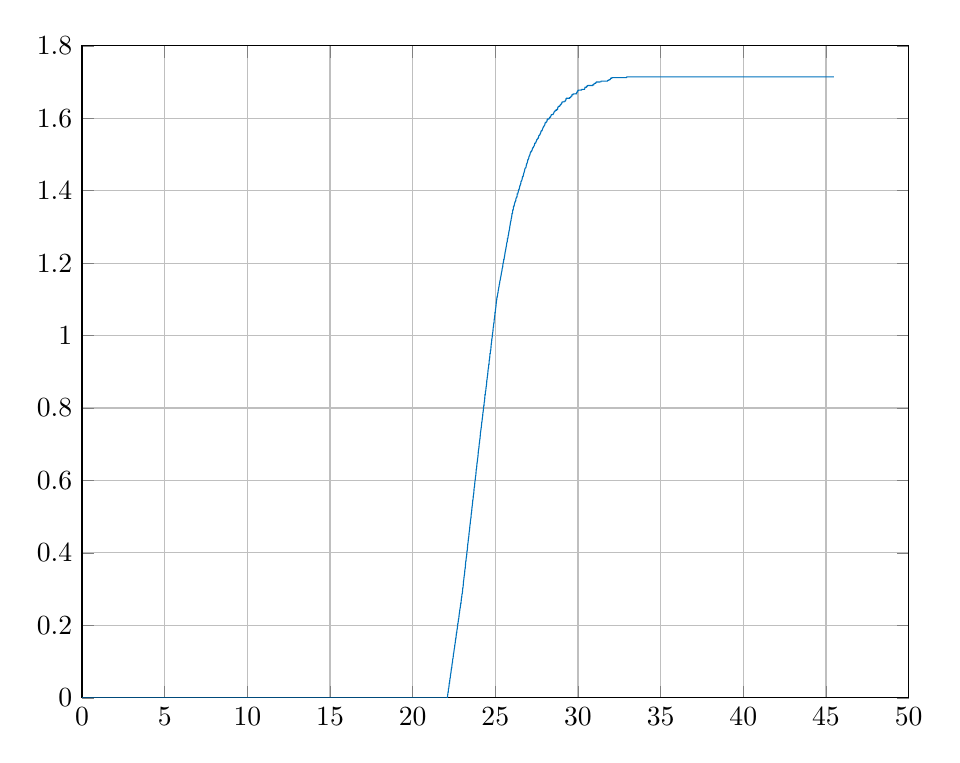
\begin{tikzpicture}

\begin{axis}[%
width=4.133in,
height=3.26in,
at={(0.693in,0.44in)},
scale only axis,
xmin=0,
xmax=50,
xmajorgrids,
ymin=0,
ymax=1.8,
ymajorgrids,
axis background/.style={fill=white}
]
\addplot [color=mycolor1,solid,forget plot]
  table[row sep=crcr]{%
0	0\\
0.017627004999999	0\\
0.0327747189999986	0\\
0.0477685379999988	0\\
0.0636867769999988	0\\
0.0818266279999986	0\\
0.0968548159999996	0\\
0.111926547	0\\
0.127790864	0\\
0.143747592	0\\
0.159650482999999	0\\
0.177841396	0\\
0.192911899999998	0\\
0.208020343999999	0\\
0.223753929	0\\
0.239864859999999	0\\
0.255788035	0\\
0.271866466	0\\
0.287787592	0\\
0.303792953	0\\
0.319799717	0\\
0.335788785999998	0\\
0.351798507999999	0\\
0.367796984999999	0\\
0.383892833999999	0\\
0.399726994999999	0\\
0.417880218999999	0\\
0.433032675999999	0\\
0.448074034	0\\
0.463872045	0\\
0.479790275999999	0\\
0.495954927999999	0\\
0.511977958999999	0\\
0.527804439999999	0\\
0.543783481999999	0\\
0.559864358999999	0\\
0.575993435999999	0\\
0.591895623	0\\
0.607806183999998	0\\
0.623805561999999	0\\
0.639878685999999	0\\
0.655862683999998	0\\
0.671809347999999	0\\
0.688007375	0\\
0.703977030999999	0\\
0.719817071999999	0\\
0.735789037999999	0\\
0.751903521	0\\
0.767862266999999	0\\
0.78380684	0\\
0.799775462999999	0\\
0.81574808	0\\
0.831793863	0\\
0.847800606999999	0\\
0.863872895	0\\
0.879949246999999	0\\
0.896461672999998	0\\
0.911939472999999	0\\
0.928073790999999	0\\
0.944029895	0\\
0.959984832999999	0\\
0.976055911999999	0\\
0.992033660999998	0\\
1.012990514	0\\
1.025009675	0\\
1.040490137	0\\
1.055992294	0\\
1.071960656	0\\
1.088198667	0\\
1.104155596	0\\
1.11988478	0\\
1.13593575	0\\
1.151771797	0\\
1.167630294	0\\
1.185782897	0\\
1.201377082	0\\
1.216831846	0\\
1.232294868	0\\
1.248046299	0\\
1.263878221	0\\
1.279828496	0\\
1.295736922	0\\
1.311727252	0\\
1.327788756	0\\
1.343763182	0\\
1.359802976	0\\
1.375801552	0\\
1.39177865	0\\
1.407700529	0\\
1.423930848	0\\
1.440279624	0\\
1.456002694	0\\
1.471926449	0\\
1.488010619	0\\
1.503817976	0\\
1.519900482	0\\
1.535805181	0\\
1.552002246	0\\
1.56821883	0\\
1.583995539	0\\
1.599878204	0\\
1.615790014	0\\
1.631877599	0\\
1.647664555	0\\
1.665701588	0\\
1.680928124	0\\
1.696404631	0\\
1.71186283	0\\
1.730252207	0\\
1.745645141	0\\
1.761083347	0\\
1.776474597	0\\
1.79196574	0\\
1.807868222	0\\
1.823795551	0\\
1.839802816	0\\
1.855789395	0\\
1.871808517	0\\
1.887929471	0\\
1.903865954	0\\
1.919657486	0\\
1.935961966	0\\
1.952033898	0\\
1.968023889	0\\
1.983856769	0\\
1.999759955	0\\
2.015796794	0\\
2.031812557	0\\
2.047764207	0\\
2.063752644	0\\
2.079965696	0\\
2.095818827	0\\
2.112126193	0\\
2.127809033	0\\
2.143827403	0\\
2.15982371	0\\
2.175876498	0\\
2.191776335	0\\
2.207786788	0\\
2.22386105	0\\
2.239829167	0\\
2.255861534	0\\
2.271812918	0\\
2.287824834	0\\
2.303867951	0\\
2.319808069	0\\
2.335757003	0\\
2.351769706	0\\
2.367820199	0\\
2.383719034	0\\
2.399745996	0\\
2.415802099	0\\
2.431804415	0\\
2.447744153	0\\
2.463769394	0\\
2.479741956	0\\
2.495743564	0\\
2.511940698	0\\
2.527858325	0\\
2.543976016	0\\
2.559815597	0\\
2.575868305	0\\
2.591871847	0\\
2.608070682	0\\
2.624005909	0\\
2.640049349	0\\
2.655665488	0\\
2.673942147	0\\
2.689472021	0\\
2.704838134	0\\
2.720318682	0\\
2.735801307	0\\
2.751804645	0\\
2.767919825	0\\
2.783806552	0\\
2.799954908	0\\
2.815892515	0\\
2.831927218	0\\
2.847739999	0\\
2.864243923	0\\
2.879977955	0\\
2.895694244	0\\
2.911711427	0\\
2.927872543	0\\
2.943880107	0\\
2.960152786	0\\
2.976136849	0\\
2.992442385	0\\
3.010645236	0\\
3.024073413	0\\
3.039995715	0\\
3.055957568	0\\
3.071891633	0\\
3.088032265	0\\
3.103986055	0\\
3.119999544	0\\
3.135817002	0\\
3.151656771	0\\
3.169655073	0\\
3.184560306	0\\
3.199850563	0\\
3.216011025	0\\
3.232002044	0\\
3.247731998	0\\
3.263960171	0\\
3.279937487	0\\
3.29590332	0\\
3.311825067	0\\
3.328017257	0\\
3.343986025	0\\
3.359980577	0\\
3.375999619	0\\
3.391820693	0\\
3.407689629	0\\
3.42366058	0\\
3.440004937	0\\
3.456107988	0\\
3.471868399	0\\
3.487793105	0\\
3.503883728	0\\
3.519863356	0\\
3.535815948	0\\
3.551801023	0\\
3.567816813	0\\
3.583756631	0\\
3.600207591	0\\
3.616034661	0\\
3.631973083	0\\
3.647802512	0\\
3.663665581	0\\
3.679625737	0\\
3.695994628	0\\
3.711881169	0\\
3.727860845	0\\
3.743966872	0\\
3.760035076	0\\
3.775954432	0\\
3.794297178	0\\
3.809654195	0\\
3.82476268	0\\
3.839869516	0\\
3.855807023	0\\
3.871868883	0\\
3.888104941	0\\
3.903784654	0\\
3.919657818	0\\
3.937701482	0\\
3.95291856	0\\
3.968301958	0\\
3.983983911	0\\
3.999825184	0\\
4.017519282	0\\
4.032710384	0\\
4.047866862	0\\
4.064139198	0\\
4.080029619	0\\
4.095882935	0\\
4.111873057	0\\
4.128136433	0\\
4.143892278	0\\
4.159739011	0\\
4.177935996	0\\
4.193345052	0\\
4.208641668	0\\
4.224113879	0\\
4.239947172	0\\
4.25597298	0\\
4.271930102	0\\
4.287987125	0\\
4.303951243	0\\
4.319947318	0\\
4.33594442	0\\
4.351974207	0\\
4.367976556	0\\
4.384053314	0\\
4.399827501	0\\
4.416341439	0\\
4.43181896	0\\
4.447804054	0\\
4.463974977	0\\
4.479937368	0\\
4.495878271	0\\
4.512020782	0\\
4.527884096	0\\
4.543892205	0\\
4.560117343	0\\
4.575878175	0\\
4.591862339	0\\
4.60795167	0\\
4.623975423	0\\
4.63998543	0\\
4.655723423	0\\
4.671695315	0\\
4.687811757	0\\
4.703935277	0\\
4.719812847	0\\
4.736035157	0\\
4.751879723	0\\
4.76798453	0\\
4.783822211	0\\
4.799956619	0\\
4.816068272	0\\
4.832021379	0\\
4.847904669	0\\
4.863997323	0\\
4.880132879	0\\
4.895649057	0\\
4.913762656	0\\
4.928748145	0\\
4.943924162	0\\
4.959808103	0\\
4.975789906	0\\
4.99176524	0\\
5.009068286	0\\
5.024370002	0\\
5.039933467	0\\
5.055988474	0\\
5.071998062	0\\
5.087819251	0\\
5.103805213	0\\
5.119851335	0\\
5.135966847	0\\
5.151649607	0\\
5.16764885	0\\
5.185692803	0\\
5.201113096	0\\
5.216486093	0\\
5.231982492	0\\
5.247898811	0\\
5.263797546	0\\
5.27980209	0\\
5.295776747	0\\
5.31182054	0\\
5.327991732	0\\
5.343874794	0\\
5.359873114	0\\
5.37587304	0\\
5.391872199	0\\
5.407690814	0\\
5.423662849	0\\
5.43987021	0\\
5.455733015	0\\
5.471794601	0\\
5.487823922	0\\
5.503824307	0\\
5.51982593	0\\
5.535817074	0\\
5.551801493	0\\
5.567802253	0\\
5.583915624	0\\
5.599790274	0\\
5.615828665	0\\
5.631818301	0\\
5.647945694	0\\
5.663646814	0\\
5.679891156	0\\
5.695861745	0\\
5.711814472	0\\
5.727862319	0\\
5.743821266	0\\
5.759807609	0\\
5.775791551	0\\
5.791800621	0\\
5.807805982	0\\
5.823799376	0\\
5.839791256	0\\
5.855824616	0\\
5.871799659	0\\
5.887755623	0\\
5.903704049	0\\
5.921724081	0\\
5.936761629	0\\
5.951810318	0\\
5.967852728	0\\
5.98379203	0\\
5.999801205	0\\
6.017264463	0\\
6.032409405	0\\
6.047793604	0\\
6.06381671	0\\
6.079849469	0\\
6.095790399	0\\
6.111870364	0\\
6.127954634	0\\
6.143857899	0\\
6.159676503	0\\
6.178057595	0\\
6.193509908	0\\
6.208640332	0\\
6.223923328	0\\
6.239998472	0\\
6.255798688	0\\
6.271888646	0\\
6.287788683	0\\
6.303821487	0\\
6.319868678	0\\
6.335758226	0\\
6.351808204	0\\
6.367935712	0\\
6.383771678	0\\
6.399881913	0\\
6.415683113	0\\
6.433990748	0\\
6.449409285	0\\
6.464666952	0\\
6.480081064	0\\
6.495982991	0\\
6.511820096	0\\
6.52779437	0\\
6.561458611	0\\
6.566951054	0\\
6.575775965	0\\
6.591698844	0\\
6.609903056	0\\
6.625018457	0\\
6.640392152	0\\
6.655669563	0\\
6.673841178	0\\
6.688906606	0\\
6.704260517	0\\
6.719812025	0\\
6.735893719	0\\
6.751819076	0\\
6.767860517	0\\
6.783908014	0\\
6.7997936	0\\
6.815864408	0\\
6.831863485	0\\
6.847906865	0\\
6.863861132	0\\
6.879676884	0\\
6.896006415	0\\
6.911657869	0\\
6.927860502	0\\
6.94369346	0\\
6.959823531	0\\
6.9758632	0\\
6.991885189	0\\
7.00948517	0\\
7.024426289	0\\
7.039677298	0\\
7.055689692	0\\
7.071722285	0\\
7.087716341	0\\
7.103810163	0\\
7.119807335	0\\
7.135860429	0\\
7.151679383	0\\
7.167643742	0\\
7.185934224	0\\
7.201095538	0\\
7.21640644	0\\
7.231757846	0\\
7.247865384	0\\
7.263864143	0\\
7.279708539	0\\
7.295882535	0\\
7.311827324	0\\
7.327747191	0\\
7.343857996	0\\
7.35978732	0\\
7.375788366	0\\
7.391945321	0\\
7.407687765	0\\
7.425965365	0\\
7.441202461	0\\
7.45642996	0\\
7.471824818	0\\
7.487877432	0\\
7.503882822	0\\
7.519744581	0\\
7.535691337	0\\
7.551893524	0\\
7.567887389	0\\
7.583888606	0\\
7.599816401	0\\
7.615863282	0\\
7.631853937	0\\
7.647931993	0\\
7.66549047	0\\
7.680518346	0\\
7.69611649	0\\
7.711876591	0\\
7.72787203	0\\
7.743948931	0\\
7.759749242	0\\
7.775828293	0\\
7.791858556	0\\
7.80771977	0\\
7.823765762	0\\
7.839742714	0\\
7.855719797	0\\
7.87172126	0\\
7.887887059	0\\
7.90375023	0\\
7.919874387	0\\
7.935851307	0\\
7.951780743	0\\
7.967936338	0\\
7.983877699	0\\
7.999872474	0\\
8.017289673	0\\
8.032245091	0\\
8.04763903	0\\
8.065696498	0\\
8.080668024	0\\
8.095876252	0\\
8.111870934	0\\
8.127870181	0\\
8.143972467	0\\
8.159678654	0\\
8.177706287	0\\
8.192922015	0\\
8.208198169	0\\
8.223801299	0\\
8.239818151	0\\
8.255660558	0\\
8.274159738	0\\
8.289633987	0\\
8.305104366	0\\
8.320541299	0\\
8.335964807	0\\
8.351868499	0\\
8.367887245	0\\
8.383698391	0\\
8.399640567	0\\
8.417764893	0\\
8.433303919	0\\
8.448830031	0\\
8.464404805	0\\
8.479893582	0\\
8.495911026	0\\
8.511791925	0\\
8.527852687	0\\
8.543787388	0\\
8.559786545	0\\
8.575815365	0\\
8.591805957	0\\
8.607862249	0\\
8.623720291	0\\
8.639911007	0\\
8.655672235	0\\
8.671764948	0\\
8.687892562	0\\
8.703952626	0\\
8.719695361	0\\
8.735950867	0\\
8.751786448	0\\
8.767853239	0\\
8.783810831	0\\
8.799793356	0\\
8.815821188	0\\
8.83178271	0\\
8.847822609	0\\
8.863706475	0\\
8.879804456	0\\
8.895902557	0\\
8.911782706	0\\
8.927698842	0\\
8.943768055	0\\
8.959796879	0\\
8.975795059	0\\
8.991776516	0\\
9.009183798	0\\
9.024356738	0\\
9.039791547	0\\
9.055750553	0\\
9.071819048	0\\
9.087806298	0\\
9.103760237	0\\
9.119860534	0\\
9.135748083	0\\
9.151731427	0\\
9.16764455	0\\
9.1837989	0\\
9.199793517	0\\
9.21593639	0\\
9.23182003	0\\
9.2479285	0\\
9.263788822	0\\
9.279958025	0\\
9.295662011	0\\
9.311772648	0\\
9.327785396	0\\
9.343896953	0\\
9.36174587	0\\
9.37686792	0\\
9.391936599	0\\
9.407782895	0\\
9.423824204	0\\
9.439745033	0\\
9.455852901	0\\
9.471818392	0\\
9.487779052	0\\
9.503896442	0\\
9.519679327	0\\
9.537731842	0\\
9.552990903	0\\
9.568209512	0\\
9.583787635	0\\
9.599762262	0\\
9.615849664	0\\
9.631664779	0\\
9.647854574	0\\
9.663722671	0\\
9.679672128	0\\
9.695786852	0\\
9.711790344	0\\
9.727860316	0\\
9.743805837	0\\
9.759822954	0\\
9.775941206	0\\
9.79177988	0\\
9.807783946	0\\
9.823803923	0\\
9.839762147	0\\
9.855791197	0\\
9.871864011	0\\
9.887853005	0\\
9.90364736	0\\
9.921648706	0\\
9.936677319	0\\
9.951642233	0\\
9.967677502	0\\
9.983782489	0\\
9.999776034	0\\
10.017032729	0\\
10.031978272	0\\
10.047690637	0\\
10.06577541	0\\
10.080814346	0\\
10.095871258	0\\
10.111786771	0\\
10.127786199	0\\
10.143779097	0\\
10.159640141	0\\
10.177696212	0\\
10.192853838	0\\
10.208131443	0\\
10.223802675	0\\
10.239674315	0\\
10.25586475	0\\
10.271851904	0\\
10.287802486	0\\
10.303807967	0\\
10.319863643	0\\
10.335894036	0\\
10.35167594	0\\
10.367813817	0\\
10.383893406	0\\
10.399952478	0\\
10.415702439	0\\
10.431788034	0\\
10.447799307	0\\
10.463866425	0\\
10.479969056	0\\
10.495809869	0\\
10.511784245	0\\
10.527786086	0\\
10.543734214	0\\
10.560073714	0\\
10.575998573	0\\
10.591904163	0\\
10.607980956	0\\
10.623763951	0\\
10.639788313	0\\
10.655690043	0\\
10.673977748	0\\
10.689360587	0\\
10.704531717	0\\
10.719792021	0\\
10.735798239	0\\
10.75186553	0\\
10.767775791	0\\
10.783775264	0\\
10.799749044	0\\
10.815782855	0\\
10.831717566	0\\
10.847758733	0\\
10.863861364	0\\
10.879660949	0\\
10.895823336	0\\
10.911650793	0\\
10.92980154	0\\
10.945560424	0\\
10.961214712	0\\
10.976697902	0\\
10.992021073	0\\
11.009933884	0\\
11.025040045	0\\
11.040313713	0\\
11.055786283	0\\
11.071773382	0\\
11.087742231	0\\
11.103751972	0\\
11.11972356	0\\
11.135746382	0\\
11.151727239	0\\
11.167700504	0\\
11.183758031	0\\
11.199829557	0\\
11.216047419	0\\
11.232014524	0\\
11.247744406	0\\
11.263763681	0\\
11.27981097	0\\
11.29579802	0\\
11.311791158	0\\
11.327771552	0\\
11.343754788	0\\
11.359972802	0\\
11.375888118	0\\
11.392157899	0\\
11.407860489	0\\
11.42365893	0\\
11.441916249	0\\
11.457588499	0\\
11.473253783	0\\
11.488803536	0\\
11.504431502	0\\
11.519934064	0\\
11.536288165	0\\
11.551979189	0\\
11.567796525	0\\
11.583773792	0\\
11.599772218	0\\
11.615850008	0\\
11.631792206	0\\
11.647954717	0\\
11.663663578	0\\
11.681747497	0\\
11.697206305	0\\
11.712599745	0\\
11.728058099	0\\
11.743995995	0\\
11.759795626	0\\
11.775782826	0\\
11.791787054	0\\
11.807740087	0\\
11.82377295	0\\
11.83976647	0\\
11.855942387	0\\
11.871882731	0\\
11.887826409	0\\
11.903721295	0\\
11.922163025	0\\
11.937720696	0\\
11.953041426	0\\
11.968370636	0\\
11.983893938	0\\
11.999905004	0\\
12.017284458	0\\
12.032417538	0\\
12.047797457	0\\
12.063989406	0\\
12.079796247	0\\
12.095686649	0\\
12.112067325	0\\
12.127865446	0\\
12.143816259	0\\
12.159651027	0\\
12.177698274	0\\
12.192953867	0\\
12.208369859	0\\
12.223922395	0\\
12.239957659	0\\
12.255889102	0\\
12.271873441	0\\
12.287864675	0\\
12.30380106	0\\
12.319820087	0\\
12.336503449	0\\
12.351913397	0\\
12.367694297	0\\
12.383798895	0\\
12.399808599	0\\
12.415688548	0\\
12.43188638	0\\
12.44774749	0\\
12.463642034	0\\
12.479716257	0\\
12.495730589	0\\
12.511766939	0\\
12.527956128	0\\
12.543955981	0\\
12.559794459	0\\
12.575722483	0\\
12.592062439	0\\
12.607760823	0\\
12.623762671	0\\
12.639766226	0\\
12.655875988	0\\
12.671647968	0\\
12.689894019	0\\
12.705433091	0\\
12.721022436	0\\
12.736595895	0\\
12.751984769	0\\
12.768229963	0\\
12.784077096	0\\
12.800274607	0\\
12.815902278	0\\
12.831804952	0\\
12.847796557	0\\
12.863970004	0\\
12.885462958	0\\
12.897481368	0\\
12.912772037	0\\
12.928278493	0\\
12.943775676	0\\
12.959911936	0\\
12.975750846	0\\
12.991781669	0\\
13.01254802	0\\
13.024416124	0\\
13.039827555	0\\
13.055822899	0\\
13.071781674	0\\
13.09010038	0\\
13.10511796	0\\
13.120279834	0\\
13.135774828	0\\
13.151665986	0\\
13.169703295	0\\
13.184865433	0\\
13.200007553	0\\
13.216155553	0\\
13.231799509	0\\
13.247914334	0\\
13.2637422	0\\
13.2797809	0\\
13.295781454	0\\
13.314162745	0\\
13.329294355	0\\
13.344380055	0\\
13.359871988	0\\
13.375699269	0\\
13.391810906	0\\
13.40772616	0\\
13.423987777	0\\
13.439753987	0\\
13.455884569	0\\
13.471795957	0\\
13.487891437	0\\
13.503819744	0\\
13.519933562	0\\
13.5358178	0\\
13.551805945	0\\
13.567884657	0\\
13.583927984	0\\
13.599823909	0\\
13.615738683	0\\
13.631861933	0\\
13.647887573	0\\
13.663681336	0\\
13.679678923	0\\
13.697775157	0\\
13.712993406	0\\
13.72813961	0\\
13.74389068	0\\
13.759725303	0\\
13.775867666	0\\
13.79185465	0\\
13.807805794	0\\
13.823863228	0\\
13.84001179	0\\
13.855669229	0\\
13.871820539	0\\
13.887863199	0\\
13.903926136	0\\
13.919693996	0\\
13.935866018	0\\
13.951712619	0\\
13.967859033	0\\
13.983821544	0\\
13.99998371	0\\
14.017401031	0\\
14.032850492	0\\
14.048055229	0\\
14.06389067	0\\
14.079861388	0\\
14.095806004	0\\
14.111874146	0\\
14.127864332	0\\
14.143658792	0\\
14.161737314	0\\
14.176606747	0\\
14.191639854	0\\
14.209825548	0\\
14.225007175	0\\
14.240200642	0\\
14.255777753	0\\
14.271952699	0\\
14.287703853	0\\
14.303878313	0\\
14.319879389	0\\
14.335796235	0\\
14.351780679	0\\
14.367769638	0\\
14.383812038	0\\
14.400056211	0\\
14.415679017	0\\
14.431652417	0\\
14.447810581	0\\
14.549835343	0\\
14.567883932	0\\
14.583028783	0\\
14.598227052	0\\
14.613992099	0\\
14.630003103	0\\
14.64597791	0\\
14.66197217	0\\
14.67782766	0\\
14.695988156	0\\
14.711244948	0\\
14.72647896	0\\
14.742313078	0\\
14.758250536	0\\
14.774059151	0\\
14.790003113	0\\
14.806165585	0\\
14.822019563	0\\
14.838105371	0\\
14.854005462	0\\
14.870046942	0\\
14.88605715	0\\
14.901879986	0\\
14.920148164	0\\
14.935448993	0\\
14.950779369	0\\
14.966098463	0\\
14.981994657	0\\
14.998048222	0\\
15.015722995	0\\
15.030955506	0\\
15.0461657	0\\
15.062008338	0\\
15.077963245	0\\
15.093960327	0\\
15.110067945	0\\
15.125987216	0\\
15.142027732	0\\
15.158057018	0\\
15.173976915	0\\
15.189969592	0\\
15.205974628	0\\
15.222033721	0\\
15.237839046	0\\
15.254080174	0\\
15.270029809	0\\
15.285944329	0\\
15.302009686	0\\
15.317968277	0\\
15.334083923	0\\
15.350038875	0\\
15.365915945	0\\
15.381981483	0\\
15.397930691	0\\
15.413814783	0\\
15.430014931	0\\
15.445987703	0\\
15.462046406	0\\
15.478054524	0\\
15.493962092	0\\
15.509984066	0\\
15.525987688	0\\
15.541971942	0\\
15.558014342	0\\
15.574018189	0\\
15.589902778	0\\
15.605971161	0\\
15.622028971	0\\
15.637985306	0\\
15.654193321	0\\
15.670030446	0\\
15.686000978	0\\
15.701995415	0\\
15.718020516	0\\
15.733943751	0\\
15.749943845	0\\
15.765963985	0\\
15.782092279	0\\
15.797959375	0\\
15.813988718	0\\
15.830073479	0\\
15.845985884	0\\
15.861895561	0\\
15.877974462	0\\
15.893959627	0\\
15.909872714	0\\
15.926041223	0\\
15.941945081	0\\
15.957984585	0\\
15.974038701	0\\
15.989988527	0\\
16.008685309	0\\
16.023937795	0\\
16.039299975	0\\
16.054581055	0\\
16.06997232	0\\
16.086109109	0\\
16.102019645	0\\
16.117919021	0\\
16.13403094	0\\
16.150088263	0\\
16.165937074	0\\
16.184047898	0\\
16.199447043	0\\
16.214637436	0\\
16.230096627	0\\
16.246064263	0\\
16.262199208	0\\
16.277968704	0\\
16.293963256	0\\
16.309968832	0\\
16.325961746	0\\
16.341966906	0\\
16.357952483	0\\
16.373974752	0\\
16.390075409	0\\
16.405939167	0\\
16.421937901	0\\
16.437899418	0\\
16.453866954	0\\
16.469993829	0\\
16.485997918	0\\
16.501991823	0\\
16.51799338	0\\
16.533955448	0\\
16.549906676	0\\
16.566134217	0\\
16.582160875	0\\
16.598096614	0\\
16.613988193	0\\
16.630037323	0\\
16.645985074	0\\
16.661840539	0\\
16.679970289	0\\
16.695042607	0\\
16.710292201	0\\
16.725973232	0\\
16.74209833	0\\
16.757955906	0\\
16.774004881	0\\
16.79017237	0\\
16.80613542	0\\
16.822120615	0\\
16.837949952	0\\
16.854034348	0\\
16.870082266	0\\
16.886018279	0\\
16.902144429	0\\
16.918020177	0\\
16.933977524	0\\
16.950000057	0\\
16.965987094	0\\
16.981977885	0\\
16.998000683	0\\
17.015391868	0\\
17.030454143	0\\
17.04596982	0\\
17.061964066	0\\
17.077945328	0\\
17.09398425	0\\
17.109964299	0\\
17.126004023	0\\
17.142068874	0\\
17.158040293	0\\
17.17403095	0\\
17.190065513	0\\
17.206143514	0\\
17.222087416	0\\
17.238095799	0\\
17.254090716	0\\
17.270008459	0\\
17.28611973	0\\
17.302142566	0\\
17.318139678	0\\
17.334151163	0\\
17.350127293	0\\
17.365938525	0\\
17.381904401	0\\
17.400379986	0\\
17.415299264	0\\
17.430387247	0\\
17.446147817	0\\
17.462092222	0\\
17.4782019	0\\
17.493970848	0\\
17.50986969	0\\
17.526107337	0\\
17.541999823	0\\
17.557967356	0\\
17.574030976	0\\
17.590012639	0\\
17.605950663	0\\
17.621969539	0\\
17.637941219	0\\
17.654074415	0\\
17.6698351	0\\
17.687979974	0\\
17.703261456	0\\
17.718304107	0\\
17.733927875	0\\
17.749959904	0\\
17.765940179	0\\
17.781924097	0\\
17.797913652	0\\
17.814003249	0\\
17.829902438	0\\
17.846086212	0\\
17.862094533	0\\
17.878132252	0\\
17.894149801	0\\
17.909994519	0\\
17.926020474	0\\
17.942101419	0\\
17.958068077	0\\
17.97404948	0\\
17.990057446	0\\
18.008500996	0\\
18.023565164	0\\
18.038760476	0\\
18.053959761	0\\
18.069906127	0\\
18.085848492	0\\
18.10195646	0\\
18.118017002	0\\
18.134006156	0\\
18.14999943	0\\
18.165845217	0\\
18.182095405	0\\
18.198230751	0\\
18.213866039	0\\
18.229867737	0\\
18.245857485	0\\
18.261911033	0\\
18.278030547	0\\
18.294004462	0\\
18.309912172	0\\
18.325919323	0\\
18.341995269	0\\
18.35794546	0\\
18.373969613	0\\
18.390000723	0\\
18.405971824	0\\
18.422006246	0\\
18.437909932	0\\
18.45399883	0\\
18.469970824	0\\
18.48599559	0\\
18.501907135	0\\
18.518041422	0\\
18.533999076	0\\
18.550062476	0\\
18.568264718	0\\
18.583290984	0\\
18.598352492	0\\
18.613993172	0\\
18.629979921	0\\
18.645961674	0\\
18.661829833	0\\
18.680035299	0\\
18.695102175	0\\
18.710207522	0\\
18.726177458	0\\
18.742354418	0\\
18.757942469	0\\
18.774014641	0\\
18.789964907	0\\
18.805912398	0\\
18.821954146	0\\
18.837950292	0\\
18.854001226	0\\
18.869999997	0\\
18.885966946	0\\
18.90196255	0\\
18.917861052	0\\
18.935822449	0\\
18.950638963	0\\
18.965781292	0\\
18.982110432	0\\
18.998258685	0\\
19.015808096	0\\
19.031137179	0\\
19.046655657	0\\
19.062099346	0\\
19.078143745	0\\
19.093974721	0\\
19.110150534	0\\
19.126057021	0\\
19.142351367	0\\
19.15809924	0\\
19.173818747	0\\
19.189969945	0\\
19.206114932	0\\
19.22197526	0\\
19.237951369	0\\
19.253970061	0\\
19.270017728	0\\
19.286039886	0\\
19.302006463	0\\
19.318039986	0\\
19.333990572	0\\
19.349976043	0\\
19.365969718	0\\
19.381996533	0\\
19.397968013	0\\
19.413901465	0\\
19.430006122	0\\
19.44636627	0\\
19.462151547	0\\
19.478012764	0\\
19.494153307	0\\
19.510145147	0\\
19.525851562	0\\
19.54212968	0\\
19.558217483	0\\
19.574136854	0\\
19.590149402	0\\
19.605923827	0\\
19.624143367	0\\
19.639201151	0\\
19.654274541	0\\
19.669920007	0\\
19.6880254	0\\
19.703131139	0\\
19.718182009	0\\
19.733913939	0\\
19.75259865	0\\
19.768183303	0\\
19.783572053	0\\
19.799139657	0\\
19.814625968	0\\
19.830057344	0\\
19.846008261	0\\
19.862075077	0\\
19.87801487	0\\
19.893969892	0\\
19.909856561	0\\
19.927896709	0\\
19.943067886	0\\
19.958254092	0\\
19.974178504	0\\
19.990041211	0\\
20.008710191	0\\
20.023786188	0\\
20.039136428	0\\
20.054206112	0\\
20.069911308	0\\
20.085890881	0\\
20.101978188	0\\
20.117907526	0\\
20.133983513	0\\
20.149888292	0\\
20.165965836	0\\
20.181865227	0\\
20.197906423	0\\
20.214000762	0\\
20.230045588	0\\
20.246017869	0\\
20.261894291	0\\
20.278094385	0\\
20.294031558	0\\
20.310051108	0\\
20.325982734	0\\
20.341990245	0\\
20.35806324	0\\
20.373930423	0\\
20.390024334	0\\
20.406069486	0\\
20.422005821	0\\
20.438005038	0\\
20.453990354	0\\
20.469985883	0\\
20.485855899	0\\
20.501965078	0\\
20.518022548	0\\
20.533998131	0\\
20.550138038	0\\
20.565919362	0\\
20.581997572	0\\
20.597998347	0\\
20.613998242	0\\
20.629996176	0\\
20.645976891	0\\
20.66183582	0\\
20.679901165	0\\
20.69485835	0\\
20.710065534	0\\
20.725814183	0\\
20.741958229	0\\
20.757995682	0\\
20.77400388	0\\
20.789970152	0\\
20.805860908	0\\
20.821985973	0\\
20.838030286	0\\
20.854034467	0\\
20.869979281	0\\
20.885994151	0\\
20.902059824	0\\
20.917974412	0\\
20.93411137	0\\
20.950076019	0\\
20.966008574	0\\
20.982002053	0\\
20.99798134	0\\
21.015280377	0\\
21.030340307	0\\
21.045867314	0\\
21.062044499	0\\
21.0779569	0\\
21.093965629	0\\
21.109975109	0\\
21.126032133	0\\
21.141992186	0\\
21.158072843	0\\
21.173953539	0\\
21.189840249	0\\
21.205982685	0\\
21.221989009	0\\
21.237925664	0\\
21.253992806	0\\
21.270012735	0\\
21.285955324	0\\
21.30195832	0\\
21.318057649	0\\
21.334068011	0\\
21.349841656	0\\
21.3681961	0\\
21.383452675	0\\
21.398792258	0\\
21.413842567	0\\
21.431881907	0\\
21.447120497	0\\
21.462173096	0\\
21.477987946	0\\
21.493970664	0\\
21.509785736	0\\
21.525805994	0\\
21.541812183	0\\
21.557847458	0\\
21.574015833	0\\
21.589993462	0\\
21.605940295	0\\
21.621986629	0\\
21.637964373	0\\
21.654028412	0\\
21.669917721	0\\
21.685960281	0\\
21.702003267	0\\
21.718056116	0\\
21.734039232	0\\
21.749953862	0\\
21.765856111	0\\
21.781957784	0\\
21.797909809	0\\
21.813964076	0\\
21.830002262	0\\
21.845939624	0\\
21.861940685	0\\
21.878178528	0\\
21.894189367	0\\
21.90996144	0\\
21.925829928	0\\
21.944078905	0\\
21.959422342	0\\
21.974873428	0\\
21.990389389	0\\
22.00950892	0\\
22.021926764	0\\
22.04018348	0\\
22.055329988	0\\
22.070332851	0\\
22.086130933	0\\
22.101961057	0\\
22.117941344	0.00785127862426322\\
22.133967159	0.0137399061825191\\
22.149963124	0.0157022896329539\\
22.165836722	0.0250897814152738\\
22.183917149	0.0270529853931383\\
22.199138082	0.0329409414013018\\
22.214419394	0.0407918231279506\\
22.229953412	0.040791837724265\\
22.245998332	0.0486424541047916\\
22.261953535	0.0545307509700575\\
22.277974296	0.0564926775273161\\
22.293967986	0.0658830664062457\\
22.309994309	0.067845853073726\\
22.326128483	0.0737336435143141\\
22.342172236	0.081583796253318\\
22.358185655	0.081583796253318\\
22.374258449	0.0894336985127003\\
22.390111976	0.0953214016211107\\
22.406047254	0.0972834474134379\\
22.421835463	0.106676465772583\\
22.439917654	0.108639357416387\\
22.454915332	0.114526304037079\\
22.470366095	0.122375865795524\\
22.485972971	0.124338419292223\\
22.501978648	0.130225163497416\\
22.518065067	0.136112341017541\\
22.53412175	0.138074062873448\\
22.550092187	0.146695767836924\\
22.566144725	0.149432563793814\\
22.582119752	0.155319213446622\\
22.598150331	0.163168027248079\\
22.614104606	0.163168037801786\\
22.630113696	0.171016595579015\\
22.64606504	0.178865003127548\\
22.662109509	0.178865003127548\\
22.677829424	0.18709964726585\\
22.695838741	0.190226093873378\\
22.710936981	0.196112026623433\\
22.726508434	0.203960242090493\\
22.742163898	0.20592246659536\\
22.758095942	0.211808196033375\\
22.774101655	0.217694363677436\\
22.790153697	0.219655635748318\\
22.806042912	0.227503275138496\\
22.82210108	0.232981681613742\\
22.838149333	0.236905138526557\\
22.854155898	0.244752506594958\\
22.870005575	0.246714558898349\\
22.888615916	0.252599716381474\\
22.904163707	0.260446770387932\\
22.919953994	0.260446638418113\\
22.935306033	0.268293294664811\\
22.950476469	0.275736625084447\\
22.966030687	0.277697922769776\\
22.981959486	0.28554478766261\\
22.997959379	0.287506655135475\\
23.015434204	0.293391365324073\\
23.03066269	0.303198085108729\\
23.045980072	0.305158514615132\\
23.062005354	0.313004795006063\\
23.077954362	0.322806853616092\\
23.093922223	0.326728590179889\\
23.110017774	0.334574598053904\\
23.12601888	0.33849672162187\\
23.141975175	0.344380847898498\\
23.157860699	0.35418698725554\\
23.173906994	0.356146986184332\\
23.189991009	0.364385647285716\\
23.206018119	0.375759169167122\\
23.221962918	0.377719624557918\\
23.238063439	0.385565037547362\\
23.253957143	0.389486824022851\\
23.269989094	0.395370429153705\\
23.286294059	0.40517547825776\\
23.302125476	0.407135553983194\\
23.318132656	0.415765280604907\\
23.334144868	0.424789749406326\\
23.350150334	0.428710707922131\\
23.366167327	0.436555349626683\\
23.382130608	0.442438177256162\\
23.397973581	0.446359823933783\\
23.413870656	0.456164249605717\\
23.429991138	0.460085089341889\\
23.445984229	0.466760703939054\\
23.462060655	0.475780878324279\\
23.477971812	0.479701635873331\\
23.493814715	0.487545585163315\\
23.510027657	0.493427894341451\\
23.526093861	0.497349198762784\\
23.542008549	0.507152506721352\\
23.558237995	0.511073313361534\\
23.574150927	0.518144203021253\\
23.590303447	0.526772155153413\\
23.606307861	0.530692405777862\\
23.62204964	0.538535675338915\\
23.63795933	0.546378074647124\\
23.654030961	0.548338335577017\\
23.669867623	0.558141040097347\\
23.687955235	0.56206096265988\\
23.702832025	0.569134066337665\\
23.717823661	0.579723290755535\\
23.735877231	0.581683024213981\\
23.751042424	0.589525556738395\\
23.766371617	0.597367374082126\\
23.781989215	0.601286808660245\\
23.798125872	0.609128781861122\\
23.814042813	0.613049031628234\\
23.82999572	0.620518545788995\\
23.846075773	0.630713975142319\\
23.862178723	0.632673450758777\\
23.877992626	0.640515284928928\\
23.893926324	0.64835625851207\\
23.912274699	0.652275510641291\\
23.927273342	0.660116782921123\\
23.942150594	0.664036248299273\\
23.958241564	0.671508737748115\\
23.974143546	0.681704339528136\\
23.99018328	0.685624119729503\\
24.00882427	0.691504737439855\\
24.021996069	0.699345170397478\\
24.037985745	0.703263683976945\\
24.054141427	0.711104355304105\\
24.07015233	0.715426065884544\\
24.086139861	0.722499137467607\\
24.102060826	0.732694529597334\\
24.118056555	0.736613944971481\\
24.134039496	0.742493933159988\\
24.149976061	0.746413069812554\\
24.165824411	0.754252043745649\\
24.183897216	0.76209186367097\\
24.199162163	0.764453553245616\\
24.214470152	0.773091802531136\\
24.229936006	0.775844466502865\\
24.24597126	0.785643222310311\\
24.262008849	0.789563544172083\\
24.278003606	0.795441763545713\\
24.29399048	0.80523960904501\\
24.30998886	0.805239463110334\\
24.325939177	0.815441523072991\\
24.341970888	0.817801986781512\\
24.357978494	0.826437094921944\\
24.373945794	0.836632650146669\\
24.390006856	0.83663249282639\\
24.406174199	0.846429915731393\\
24.423597158	0.848388573442526\\
24.438593907	0.856226819670301\\
24.454275796	0.860549784045713\\
24.470400782	0.866428494237947\\
24.486261537	0.87702721451478\\
24.501878678	0.879783233487687\\
24.518134693	0.887621513883324\\
24.534146301	0.89153956256415\\
24.549976292	0.899376172890111\\
24.568282425	0.907619633296385\\
24.583750459	0.909577881481023\\
24.599238659	0.919373630024347\\
24.614642705	0.919776209312703\\
24.630173366	0.930772617313984\\
24.646015703	0.93469095492048\\
24.662028506	0.940568195834276\\
24.677836795	0.950363941109519\\
24.6941934	0.950769954517114\\
24.7102898	0.960565037963317\\
24.72609029	0.960565037963317\\
24.741981628	0.970763613444153\\
24.75795886	0.979001058371546\\
24.774110673	0.981761442878117\\
24.789983544	0.991556045442276\\
24.805951435	0.993513924163475\\
24.822101464	1.00175780781254\\
24.837990216	1.00763369158975\\
24.853951563	1.01155169039534\\
24.869959675	1.02175034221416\\
24.885926825	1.02370832445939\\
24.901952703	1.03274975139498\\
24.917888371	1.03470765897788\\
24.933961511	1.04450164578881\\
24.950143271	1.04882687136628\\
24.966136189	1.05470272082376\\
24.982058863	1.06449635504676\\
24.998100582	1.06449535625881\\
25.015726912	1.07469394720375\\
25.031227206	1.07745875596771\\
25.046564294	1.0856952883804\\
25.062210537	1.09393830445071\\
25.078146009	1.09589703273914\\
25.094094021	1.10568962426776\\
25.110139012	1.10568962426776\\
25.125984792	1.10960559156257\\
25.142123309	1.11548228635072\\
25.158092774	1.11784613643628\\
25.173878966	1.12372104226002\\
25.191934569	1.12763857882228\\
25.207279493	1.1323686274675\\
25.222658502	1.13513297493122\\
25.238100056	1.14100830386099\\
25.25410012	1.14296652896665\\
25.269977706	1.14884206801765\\
25.286054575	1.1527582450762\\
25.301943803	1.15471632146742\\
25.317981367	1.1605917888675\\
25.334009234	1.16296121754956\\
25.349971177	1.16687686372753\\
25.366031117	1.17275368229686\\
25.382129388	1.17511724589796\\
25.397950653	1.17903267116144\\
25.413946029	1.18490948973077\\
25.429963384	1.18727093060823\\
25.445931732	1.19003431031321\\
25.462031643	1.19828001590873\\
25.478143765	1.20023717771738\\
25.493983977	1.20415442192222\\
25.509956394	1.21002932040981\\
25.525956864	1.21002932040981\\
25.544271731	1.2159035046616\\
25.559780267	1.21982131322996\\
25.575209112	1.22373663512986\\
25.590785637	1.23002415175175\\
25.606215089	1.23238911008161\\
25.622123666	1.23630435997286\\
25.638233995	1.24022245025375\\
25.654325982	1.24494499292027\\
25.669878516	1.24730579462239\\
25.687939182	1.25513948708503\\
25.703350162	1.25709603186533\\
25.71910206	1.25946776880145\\
25.734660405	1.26730138913622\\
25.750114066	1.26730132289212\\
25.766200085	1.27121635639977\\
25.782254781	1.2770931749691\\
25.798597118	1.27904968727294\\
25.814206421	1.28492365853448\\
25.830422906	1.28924772529532\\
25.846613086	1.29120401408365\\
25.862033245	1.29553578554303\\
25.877858309	1.30221722606491\\
25.893980339	1.30457630886153\\
25.909960155	1.31045252450494\\
25.926957206	1.31436776545128\\
25.942208311	1.31632606938097\\
25.958142663	1.32220034199474\\
25.9741329	1.32415907028318\\
25.990106016	1.32848895492536\\
26.008723096	1.33632207286237\\
26.023984762	1.33632207286237\\
26.03907901	1.33828037679206\\
26.054210411	1.34651982130041\\
26.069973258	1.34651982130041\\
26.085983395	1.34888233246912\\
26.101992023	1.35711835847531\\
26.118098549	1.35752085624774\\
26.13402451	1.35752085624774\\
26.150145017	1.36143552792397\\
26.166202315	1.36535361820487\\
26.181926588	1.36772782843069\\
26.197825344	1.36968419617723\\
26.213968774	1.36968419617723\\
26.230007942	1.37164250010692\\
26.2462218	1.37751695813436\\
26.26197075	1.3794756864228\\
26.27800855	1.38143205416934\\
26.29399546	1.38143205416934\\
26.309973514	1.38339035809903\\
26.325949393	1.39122354441491\\
26.341985309	1.39122354441491\\
26.357988565	1.39122354441491\\
26.374014433	1.39554447428362\\
26.389953353	1.39750348428459\\
26.406062339	1.40183677479033\\
26.421928828	1.40379314253687\\
26.438002213	1.40379314253687\\
26.454017871	1.40615565370558\\
26.469965987	1.4100710314531\\
26.485967785	1.41439167971177\\
26.502053418	1.4147941774842\\
26.518007283	1.41675054523074\\
26.534274336	1.41870884916044\\
26.550272431	1.42458330718787\\
26.566023226	1.42654203547631\\
26.58208961	1.42654203547631\\
26.59801713	1.42849840322286\\
26.61387508	1.43087218908993\\
26.629859495	1.43479027937082\\
26.646118091	1.4387053754058\\
26.661982833	1.4387053754058\\
26.677845798	1.4387053754058\\
26.694011887	1.44262004708204\\
26.710089602	1.44653813736293\\
26.726028053	1.44849686565137\\
26.742071399	1.45085949159039\\
26.758115558	1.45281779552008\\
26.774078338	1.4567331732676\\
26.790009521	1.46065098183596\\
26.82420186	1.46302283151988\\
26.840055797	1.46302283151988\\
26.856138485	1.46538534268859\\
26.872154041	1.46970356012641\\
26.888128345	1.47402386646721\\
26.904291859	1.47402386646721\\
26.920152485	1.47598023421375\\
26.936261105	1.47793853814344\\
26.952249521	1.48185662842434\\
26.968189533	1.48577172445932\\
26.984202402	1.48577172445932\\
27.000239575	1.48772809220586\\
27.017875249	1.48968639613555\\
27.033201552	1.49360448641645\\
27.04847035	1.49556321470489\\
27.064208636	1.49597869664227\\
27.080181323	1.49793506438881\\
27.09619155	1.4998933683185\\
27.112169985	1.50381116497367\\
27.128163655	1.50617553624511\\
27.144193793	1.50617553624511\\
27.160291088	1.50813155601005\\
27.176287835	1.50813092216191\\
27.19224899	1.51008915515634\\
27.208237713	1.51008902979328\\
27.224193206	1.51204686384811\\
27.240231931	1.5159621008587\\
27.256230929	1.51792048248189\\
27.272256267	1.51791966076318\\
27.288339309	1.51832485263148\\
27.304205784	1.52028122037803\\
27.320185964	1.52223859739358\\
27.336048126	1.52264275438761\\
27.354413593	1.52460141209874\\
27.369506422	1.52696398326319\\
27.384786671	1.53087841815766\\
27.400357317	1.53087841815766\\
27.416054365	1.53129351683016\\
27.432146024	1.53129319027087\\
27.44829574	1.5332510676943\\
27.464257377	1.53520696198096\\
27.48018644	1.53716506214102\\
27.49638315	1.53912357851855\\
27.512384347	1.54108117728076\\
27.528245291	1.54108067110683\\
27.54429174	1.54303703885338\\
27.560181685	1.54303670492662\\
27.576267849	1.54499383358601\\
27.604166083	1.54499359476493\\
27.609590072	1.54695189869462\\
27.624652567	1.55086560167501\\
27.640104876	1.55282323112463\\
27.656218918	1.55282323112463\\
27.672144122	1.55282209166875\\
27.690239127	1.55477813063775\\
27.705572301	1.55673565099916\\
27.720663371	1.55673479744026\\
27.736222189	1.55869216383862\\
27.752204805	1.56106068459876\\
27.7682205	1.56497425623554\\
27.784231253	1.56538885207858\\
27.800232776	1.56538885207858\\
27.816277561	1.56538823056644\\
27.832228735	1.56734463062105\\
27.848192938	1.5693009983676\\
27.864220409	1.57125868233226\\
27.88022145	1.5732151872799\\
27.896196779	1.57517277917298\\
27.912416578	1.575582180236\\
27.928130516	1.57753779331265\\
27.944363483	1.5779459246253\\
27.960354396	1.57990308643395\\
27.976266141	1.58031060678323\\
27.992354991	1.58226815448351\\
28.010317739	1.58618232836035\\
28.025570523	1.58813881655076\\
28.040776608	1.58813854841885\\
28.056204647	1.58813854841885\\
28.072256814	1.58813788525568\\
28.088227075	1.59009422662285\\
28.10417686	1.59009422662285\\
28.120219426	1.59205099222989\\
28.136218518	1.59596432775213\\
28.152204079	1.59596432775213\\
28.1681	1.59792071546239\\
28.186075815	1.59791992846056\\
28.201494755	1.59791992846056\\
28.217019843	1.59791945148064\\
28.232499018	1.59791863501549\\
28.248598692	1.59833373818359\\
28.264349226	1.60029010593014\\
28.280216946	1.60224544035278\\
28.296199761	1.60224505176239\\
28.312224711	1.60224505176239\\
28.32829308	1.60420086072281\\
28.344370981	1.6042004623113\\
28.360170347	1.60615776771993\\
28.376183754	1.60811364498888\\
28.392159128	1.61006900332649\\
28.408213851	1.61006900332649\\
28.424047027	1.61006791487265\\
28.442152299	1.61006688570239\\
28.457503254	1.61006688570239\\
28.472837234	1.61006577748735\\
28.48827315	1.61006472855578\\
28.504353942	1.61202109630232\\
28.520258024	1.61397678305309\\
28.536148866	1.61439101821638\\
28.552044834	1.61634796417794\\
28.570327178	1.61830463264388\\
28.585875113	1.61830346224091\\
28.601378623	1.62025945573094\\
28.616782657	1.62025945573094\\
28.632228728	1.62025783368389\\
28.648216647	1.62221359995602\\
28.664133734	1.62221359995602\\
28.682233113	1.62221194807588\\
28.6976252	1.62221133666123\\
28.713258265	1.62416741386993\\
28.728491445	1.62416633042899\\
28.744362362	1.62416503801845\\
28.760403564	1.62416503801845\\
28.776390283	1.62849236933316\\
28.792429702	1.63044805581746\\
28.808384142	1.63240435101892\\
28.824460213	1.6324038788485\\
28.840357625	1.63240201965594\\
28.856485799	1.63323230060423\\
28.872313258	1.63323181842155\\
28.888374846	1.63323099422841\\
28.904365043	1.63560143744417\\
28.920084053	1.63560143744417\\
28.938521498	1.63755581372718\\
28.953727864	1.6375554216553\\
28.969131518	1.6375554216553\\
28.984528059	1.63951027732583\\
29.000462282	1.64146624298813\\
29.018208026	1.64146624298813\\
29.033643441	1.64342116733954\\
29.049020729	1.64537651544325\\
29.064242225	1.64537632098188\\
29.080293536	1.64537522076434\\
29.096202498	1.64537418097772\\
29.112214244	1.64537397668279\\
29.128131414	1.64537337117902\\
29.14423229	1.64537337117902\\
29.160200101	1.64537315705053\\
29.176175523	1.64732788816844\\
29.192215018	1.64732788816844\\
29.208229523	1.6473276642064\\
29.224205196	1.64732696518002\\
29.240204173	1.64732696518002\\
29.256198795	1.64928311511257\\
29.27229523	1.65319510833906\\
29.288231046	1.65319439918142\\
29.304236387	1.65515025786108\\
29.320216422	1.65514994138896\\
29.336256731	1.65514922210009\\
29.352207138	1.65514922210009\\
29.368156733	1.65514889573485\\
29.384198641	1.65514816631478\\
29.402505526	1.65514816631478\\
29.417443465	1.65514783005644\\
29.433198383	1.65514709050518\\
29.448257297	1.65514709050518\\
29.464234403	1.65514674435375\\
29.480087665	1.65514599467132\\
29.496189775	1.65710170736706\\
29.51219472	1.65710127824123\\
29.528189673	1.65710051842766\\
29.544219038	1.65710051842766\\
29.560237254	1.65905491113776\\
29.576259233	1.65905491113776\\
29.592225284	1.66101028999383\\
29.6082982	1.66101028999383\\
29.624230335	1.66100984096273\\
29.640214467	1.66492099564357\\
29.65621828	1.66492099564357\\
29.6730843	1.66492053665986\\
29.688333183	1.66491967253787\\
29.704187607	1.66687509255089\\
29.720048214	1.66687455029498\\
29.736299499	1.6668736759824\\
29.752199897	1.6668736759824\\
29.768192724	1.66729372598083\\
29.784194232	1.66729284147769\\
29.800114535	1.66729284147769\\
29.816213529	1.66729262045066\\
29.832289671	1.66729172575699\\
29.848216564	1.66729172575699\\
29.864354526	1.66729149470503\\
29.880330591	1.66771562737531\\
29.896234412	1.66771562737531\\
29.912230755	1.66771562737531\\
29.928058857	1.67162666171463\\
29.946212079	1.67162608772562\\
29.961643069	1.67358032747871\\
29.977166413	1.67553586143916\\
29.992449789	1.6755352029744\\
30.008159032	1.6755352029744\\
30.024243039	1.67749135290695\\
30.040212875	1.67749068417927\\
30.056232915	1.67749068417927\\
30.072243627	1.67749068417927\\
30.088326549	1.6774900051887\\
30.104342103	1.6774900051887\\
30.120430943	1.6774900051887\\
30.136222901	1.67748780887492\\
30.152216551	1.67748708609663\\
30.168064293	1.67790529923281\\
30.186153376	1.67790385643691\\
30.20160143	1.67790268046867\\
30.216682272	1.67790268046867\\
30.232256215	1.67985765967068\\
30.248197015	1.67985499987917\\
30.264314886	1.67985499987917\\
30.280252595	1.67985499987917\\
30.296202996	1.67985229906036\\
30.312218576	1.67985229906036\\
30.328223	1.67985229906036\\
30.344147777	1.67984955721435\\
30.360182015	1.67984955721435\\
30.376216878	1.67984955721435\\
30.392194045	1.67984677434121\\
30.410390881	1.6818025600587\\
30.425640095	1.68571154923092\\
30.440690898	1.68570936148506\\
30.456127029	1.68570850418139\\
30.47252498	1.68570850418139\\
30.488416453	1.68570686343792\\
30.504709005	1.68570541792625\\
30.520339169	1.68766098439977\\
30.536450036	1.68765924988316\\
30.552473358	1.68765778373866\\
30.568295379	1.69003234137084\\
30.58682566	1.69003234137084\\
30.601915001	1.69044901916648\\
30.616976093	1.69044901916648\\
30.632183582	1.69044901916648\\
30.648404461	1.69044641854587\\
30.666784267	1.69044641854587\\
30.680060454	1.69044641854587\\
30.696307714	1.69044377663488\\
30.712046397	1.69044377663488\\
30.728205946	1.69044377663488\\
30.744198213	1.6904416713315\\
30.760203379	1.69044109343361\\
30.776224029	1.69044109343361\\
30.79220245	1.69043895716276\\
30.808057068	1.69043836894212\\
30.826137219	1.69043836894212\\
30.841048919	1.69043685186063\\
30.856077996	1.69043560316051\\
30.874171365	1.69043560316051\\
30.88921584	1.69043498397173\\
30.9043974	1.69238777529087\\
30.920135032	1.69238777529087\\
30.936063553	1.69238777529087\\
30.954434892	1.69238492692926\\
30.969852928	1.69433953715107\\
30.985378998	1.6962922801497\\
31.000770053	1.69628924106109\\
31.016204441	1.69628924106109\\
31.032337466	1.69628924106109\\
31.048266359	1.69628616056368\\
31.064271014	1.69628616056368\\
31.080332958	1.69824091855621\\
31.096349665	1.69823837295125\\
31.112247908	1.70019248078703\\
31.128195028	1.70019248078703\\
31.144346459	1.70019248078703\\
31.160289595	1.70019248078703\\
31.176116241	1.70019248078703\\
31.192197684	1.70019248078703\\
31.208269286	1.70019248078703\\
31.224203536	1.70019248078703\\
31.240282248	1.70019248078703\\
31.256254905	1.70019248078703\\
31.272253992	1.70019248078703\\
31.288545857	1.70019248078703\\
31.304529083	1.70019248078703\\
31.320264293	1.70019248078703\\
31.33623025	1.70061444798918\\
31.352234383	1.70061444798918\\
31.368232788	1.70061444798918\\
31.384228148	1.70061444798918\\
31.400229976	1.7025694271912\\
31.416177408	1.7025694271912\\
31.432071478	1.7025694271912\\
31.450119854	1.7025694271912\\
31.465282149	1.7025694271912\\
31.480443674	1.7025694271912\\
31.496164897	1.7025694271912\\
31.512164866	1.7025694271912\\
31.528227767	1.7025694271912\\
31.544190186	1.7025694271912\\
31.560209113	1.7025694271912\\
31.576184116	1.7025694271912\\
31.592304317	1.7025694271912\\
31.608307518	1.7025694271912\\
31.626708275	1.7025694271912\\
31.641801415	1.7025694271912\\
31.657017639	1.7025694271912\\
31.673143488	1.7025694271912\\
31.688872184	1.7025694271912\\
31.704256151	1.7025694271912\\
31.720322967	1.7025694271912\\
31.736435696	1.7025694271912\\
31.752515511	1.7025694271912\\
31.768455198	1.7025694271912\\
31.784205917	1.7025694271912\\
31.800214966	1.70452381531037\\
31.816211458	1.70452381531037\\
31.832232504	1.70452381531037\\
31.84820871	1.70452381531037\\
31.864156044	1.70452381531037\\
31.880155056	1.7064763317432\\
31.896153677	1.7064763317432\\
31.912287449	1.7064763317432\\
31.928454324	1.7064763317432\\
31.944100184	1.7064763317432\\
31.960179857	1.70843131094521\\
31.97637783	1.71038599508215\\
31.992438311	1.71038599508215\\
32.010429801	1.71038599508215\\
32.025552779	1.71038599508215\\
32.040802207	1.71038599508215\\
32.056265356	1.71234075307468\\
32.072407807	1.71234075307468\\
32.088519444	1.71234075307468\\
32.104207935	1.71234075307468\\
32.120122136	1.71234075307468\\
32.13818633	1.71234075307468\\
32.153133451	1.71234075307468\\
32.168113448	1.71234075307468\\
32.186166702	1.71234075307468\\
32.201213868	1.71234075307468\\
32.21638203	1.71234075307468\\
32.23219962	1.71234075307468\\
32.248223779	1.71234075307468\\
32.264222811	1.71234075307468\\
32.28025812	1.71234075307468\\
32.296204292	1.71234075307468\\
32.312207037	1.71234075307468\\
32.328195395	1.71234075307468\\
32.344202811	1.71234075307468\\
32.360219017	1.71234075307468\\
32.37629843	1.71234075307468\\
32.392217306	1.71234075307468\\
32.408102084	1.71234075307468\\
32.424075977	1.71234075307468\\
32.442357342	1.71234075307468\\
32.457714568	1.71234075307468\\
32.47320129	1.71234075307468\\
32.489038776	1.71234075307468\\
32.504341586	1.71234075307468\\
32.520310314	1.71234075307468\\
32.536245937	1.71234075307468\\
32.552244643	1.71234075307468\\
32.56819066	1.71234075307468\\
32.584342578	1.71234075307468\\
32.600285212	1.71234075307468\\
32.616339354	1.71234075307468\\
32.632394718	1.71234075307468\\
32.648418601	1.71234075307468\\
32.664334646	1.71234075307468\\
32.680087343	1.71234075307468\\
32.698244575	1.71234075307468\\
32.713542278	1.71234075307468\\
32.728994832	1.71234075307468\\
32.74424614	1.71234075307468\\
32.760269757	1.71234075307468\\
32.776086659	1.71234075307468\\
32.792217261	1.71234075307468\\
32.808339768	1.71234075307468\\
32.824409976	1.71234075307468\\
32.84038548	1.71234075307468\\
32.856343163	1.71234075307468\\
32.872324299	1.71234075307468\\
32.888218348	1.71234075307468\\
32.904364302	1.71234075307468\\
32.920206767	1.71234075307468\\
32.936056448	1.71234075307468\\
32.954023042	1.71429573227669\\
32.969018081	1.71429573227669\\
32.984477665	1.71429573227669\\
33.000218025	1.71429573227669\\
33.017484086	1.71429573227669\\
33.032828312	1.71429573227669\\
33.04839141	1.71429573227669\\
33.064262699	1.71429573227669\\
33.080280367	1.71429573227669\\
33.096314664	1.71429573227669\\
33.11215717	1.71429573227669\\
33.128184662	1.71429573227669\\
33.144360494	1.71429573227669\\
33.160532015	1.71429573227669\\
33.176620478	1.71429573227669\\
33.192068312	1.71429573227669\\
33.208222052	1.71429573227669\\
33.224226446	1.71429573227669\\
33.240237941	1.71429573227669\\
33.25610338	1.71429573227669\\
33.272173342	1.71429573227669\\
33.288159841	1.71429573227669\\
33.304223494	1.71429573227669\\
33.320198662	1.71429573227669\\
33.336195288	1.71429573227669\\
33.35216322	1.71429573227669\\
33.368203641	1.71429573227669\\
33.384190375	1.71429573227669\\
33.400212168	1.71429573227669\\
33.416151309	1.71429573227669\\
33.432061669	1.71429573227669\\
33.448044139	1.71429573227669\\
33.46435132	1.71429573227669\\
33.480346788	1.71429573227669\\
33.496320568	1.71429573227669\\
33.512240475	1.71429573227669\\
33.528244047	1.71429573227669\\
33.544355113	1.71429573227669\\
33.560217946	1.71429573227669\\
33.578582296	1.71429573227669\\
33.593882685	1.71429573227669\\
33.609128135	1.71429573227669\\
33.624394116	1.71429573227669\\
33.640407836	1.71429573227669\\
33.656354089	1.71429573227669\\
33.672125017	1.71429573227669\\
33.688061059	1.71429573227669\\
33.70611954	1.71429573227669\\
33.72119985	1.71429573227669\\
33.736440961	1.71429573227669\\
33.752204359	1.71429573227669\\
33.76822298	1.71429573227669\\
33.784173196	1.71429573227669\\
33.800218909	1.71429573227669\\
33.81632578	1.71429573227669\\
33.832293796	1.71429573227669\\
33.848268188	1.71429573227669\\
33.864199667	1.71429573227669\\
33.880391204	1.71429573227669\\
33.896354415	1.71429573227669\\
33.912464127	1.71429573227669\\
33.929308748	1.71429573227669\\
33.944226787	1.71429573227669\\
33.960233898	1.71429573227669\\
33.978675302	1.71429573227669\\
33.994285064	1.71429573227669\\
34.008682987	1.71429573227669\\
34.024379378	1.71429573227669\\
34.040363552	1.71429573227669\\
34.056224516	1.71429573227669\\
34.072203672	1.71429573227669\\
34.0882008	1.71429573227669\\
34.104504978	1.71429573227669\\
34.120267922	1.71429573227669\\
34.136354465	1.71429573227669\\
34.152476787	1.71429573227669\\
34.168131857	1.71429573227669\\
34.184070558	1.71429573227669\\
34.20221446	1.71429573227669\\
34.217671343	1.71429573227669\\
34.233123143	1.71429573227669\\
34.248608147	1.71429573227669\\
34.264257158	1.71429573227669\\
34.280370428	1.71429573227669\\
34.296367405	1.71429573227669\\
34.312261009	1.71429573227669\\
34.328360668	1.71429573227669\\
34.344224979	1.71429573227669\\
34.360207258	1.71429573227669\\
34.376222582	1.71429573227669\\
34.392219664	1.71429573227669\\
34.408234883	1.71429573227669\\
34.424096142	1.71429573227669\\
34.442417746	1.71429573227669\\
34.457820077	1.71429573227669\\
34.473012345	1.71429573227669\\
34.488341104	1.71429573227669\\
34.504366443	1.71429573227669\\
34.520259091	1.71429573227669\\
34.536353298	1.71429573227669\\
34.552311958	1.71429573227669\\
34.568351447	1.71429573227669\\
34.584327061	1.71429573227669\\
34.600368073	1.71429573227669\\
34.616360129	1.71429573227669\\
34.632716264	1.71429573227669\\
34.648343674	1.71429573227669\\
34.664416399	1.71429573227669\\
34.680153993	1.71429573227669\\
34.696099308	1.71429573227669\\
34.712071903	1.71429573227669\\
34.728347173	1.71429573227669\\
34.74423875	1.71429573227669\\
34.760367156	1.71429573227669\\
34.776326984	1.71429573227669\\
34.792322813	1.71429573227669\\
34.808365229	1.71429573227669\\
34.824354368	1.71429573227669\\
34.840415375	1.71429573227669\\
34.856390944	1.71429573227669\\
34.872379928	1.71429573227669\\
34.888268681	1.71429573227669\\
34.904394404	1.71429573227669\\
34.92010203	1.71429573227669\\
34.938248441	1.71429573227669\\
34.953723662	1.71429573227669\\
34.96925738	1.71429573227669\\
34.984739145	1.71429573227669\\
35.000341574	1.71429573227669\\
35.017844191	1.71429573227669\\
35.033066865	1.71429573227669\\
35.048638723	1.71429573227669\\
35.064616773	1.71429573227669\\
35.080266344	1.71429573227669\\
35.096425282	1.71429573227669\\
35.112376395	1.71429573227669\\
35.128256717	1.71429573227669\\
35.144347203	1.71429573227669\\
35.160325357	1.71429573227669\\
35.176056334	1.71429573227669\\
35.194160723	1.71429573227669\\
35.209527713	1.71429573227669\\
35.224991467	1.71429573227669\\
35.240368024	1.71429573227669\\
35.25622996	1.71429573227669\\
35.272234624	1.71429573227669\\
35.288201744	1.71429573227669\\
35.304205607	1.71429573227669\\
35.32021406	1.71429573227669\\
35.33619218	1.71429573227669\\
35.352193652	1.71429573227669\\
35.368357216	1.71429573227669\\
35.384378524	1.71429573227669\\
35.400349477	1.71429573227669\\
35.416306567	1.71429573227669\\
35.432110863	1.71429573227669\\
35.449124645	1.71429573227669\\
35.46467216	1.71429573227669\\
35.480431897	1.71429573227669\\
35.496467471	1.71429573227669\\
35.512271351	1.71429573227669\\
35.528348968	1.71429573227669\\
35.544380403	1.71429573227669\\
35.560349913	1.71429573227669\\
35.576420548	1.71429573227669\\
35.59236947	1.71429573227669\\
35.60825153	1.71429573227669\\
35.624415603	1.71429573227669\\
35.640375476	1.71429573227669\\
35.65624676	1.71429573227669\\
35.672109467	1.71429573227669\\
35.688056072	1.71429573227669\\
35.704116543	1.71429573227669\\
35.72035962	1.71429573227669\\
35.736348685	1.71429573227669\\
35.752166967	1.71429573227669\\
35.768271849	1.71429573227669\\
35.784356489	1.71429573227669\\
35.800368673	1.71429573227669\\
35.816417896	1.71429573227669\\
35.832390063	1.71429573227669\\
35.848376055	1.71429573227669\\
35.864325028	1.71429573227669\\
35.880369568	1.71429573227669\\
35.89630523	1.71429573227669\\
35.912487063	1.71429573227669\\
35.928058826	1.71429573227669\\
35.946149909	1.71429573227669\\
35.961290003	1.71429573227669\\
35.976973836	1.71429573227669\\
35.992490147	1.71429573227669\\
36.010233067	1.71429573227669\\
36.025551989	1.71429573227669\\
36.04087151	1.71429573227669\\
36.056321674	1.71429573227669\\
36.072374041	1.71429573227669\\
36.088348423	1.71429573227669\\
36.104281876	1.71429573227669\\
36.120261629	1.71429573227669\\
36.136203481	1.71429573227669\\
36.152336261	1.71429573227669\\
36.168251545	1.71429573227669\\
36.184042226	1.71429573227669\\
36.202191501	1.71429573227669\\
36.217724126	1.71429573227669\\
36.23303734	1.71429573227669\\
36.248418592	1.71429573227669\\
36.264456597	1.71429573227669\\
36.280341135	1.71429573227669\\
36.296339194	1.71429573227669\\
36.312361198	1.71429573227669\\
36.328296991	1.71429573227669\\
36.34433187	1.71429573227669\\
36.36036538	1.71429573227669\\
36.376230428	1.71429573227669\\
36.392369712	1.71429573227669\\
36.408466866	1.71429573227669\\
36.425052086	1.71429573227669\\
36.44005876	1.71429573227669\\
36.456030197	1.71429573227669\\
36.472318811	1.71429573227669\\
36.488347511	1.71429573227669\\
36.504327129	1.71429573227669\\
36.520157616	1.71429573227669\\
36.536200861	1.71429573227669\\
36.552363564	1.71429573227669\\
36.568212486	1.71429573227669\\
36.584208591	1.71429573227669\\
36.60017978	1.71429573227669\\
36.616212458	1.71429573227669\\
36.632210652	1.71429573227669\\
36.648205895	1.71429573227669\\
36.666493918	1.71429573227669\\
36.680137231	1.71429573227669\\
36.696158731	1.71429573227669\\
36.712334095	1.71429573227669\\
36.728406377	1.71429573227669\\
36.744353534	1.71429573227669\\
36.760319835	1.71429573227669\\
36.776373282	1.71429573227669\\
36.792285141	1.71429573227669\\
36.808212205	1.71429573227669\\
36.824178919	1.71429573227669\\
36.840335898	1.71429573227669\\
36.856329969	1.71429573227669\\
36.872341554	1.71429573227669\\
36.888345943	1.71429573227669\\
36.904283044	1.71429573227669\\
36.920113466	1.71429573227669\\
36.936082217	1.71429573227669\\
36.952375015	1.71429573227669\\
36.968374884	1.71429573227669\\
36.984354422	1.71429573227669\\
37.000336225	1.71429573227669\\
37.018081803	1.71429573227669\\
37.033592829	1.71429573227669\\
37.049035816	1.71429573227669\\
37.064468079	1.71429573227669\\
37.080408168	1.71429573227669\\
37.096212605	1.71429573227669\\
37.112365138	1.71429573227669\\
37.128361945	1.71429573227669\\
37.144222062	1.71429573227669\\
37.16020189	1.71429573227669\\
37.176092354	1.71429573227669\\
37.194183109	1.71429573227669\\
37.20974485	1.71429573227669\\
37.225099713	1.71429573227669\\
37.240583219	1.71429573227669\\
37.256356044	1.71429573227669\\
37.272444222	1.71429573227669\\
37.288370485	1.71429573227669\\
37.304326313	1.71429573227669\\
37.320573041	1.71429573227669\\
37.336477118	1.71429573227669\\
37.352340878	1.71429573227669\\
37.368342702	1.71429573227669\\
37.384195049	1.71429573227669\\
37.400157129	1.71429573227669\\
37.41842252	1.71429573227669\\
37.432473127	1.71429573227669\\
37.448030869	1.71429573227669\\
37.466061432	1.71429573227669\\
37.481234801	1.71429573227669\\
37.496608386	1.71429573227669\\
37.512394946	1.71429573227669\\
37.528272688	1.71429573227669\\
37.544393489	1.71429573227669\\
37.560361096	1.71429573227669\\
37.576304254	1.71429573227669\\
37.592387008	1.71429573227669\\
37.608418644	1.71429573227669\\
37.624225044	1.71429573227669\\
37.640215507	1.71429573227669\\
37.656354425	1.71429573227669\\
37.672319288	1.71429573227669\\
37.688060313	1.71429573227669\\
37.706047587	1.71429573227669\\
37.720939071	1.71429573227669\\
37.736396526	1.71429573227669\\
37.752364398	1.71429573227669\\
37.768248278	1.71429573227669\\
37.784325838	1.71429573227669\\
37.800426535	1.71429573227669\\
37.816403031	1.71429573227669\\
37.832364598	1.71429573227669\\
37.848481928	1.71429573227669\\
37.864246052	1.71429573227669\\
37.880208035	1.71429573227669\\
37.896185092	1.71429573227669\\
37.912236743	1.71429573227669\\
37.928131649	1.71429573227669\\
37.944328026	1.71429573227669\\
37.960155334	1.71429573227669\\
37.976369726	1.71429573227669\\
37.992336745	1.71429573227669\\
38.01017333	1.71429573227669\\
38.025608432	1.71429573227669\\
38.041179276	1.71429573227669\\
38.056607525	1.71429573227669\\
38.072350872	1.71429573227669\\
38.088436606	1.71429573227669\\
38.104261327	1.71429573227669\\
38.120264769	1.71429573227669\\
38.136334677	1.71429573227669\\
38.152242937	1.71429573227669\\
38.168175107	1.71429573227669\\
38.184090348	1.71429573227669\\
38.20254681	1.71429573227669\\
38.218017033	1.71429573227669\\
38.233504385	1.71429573227669\\
38.249092181	1.71429573227669\\
38.26464664	1.71429573227669\\
38.280215142	1.71429573227669\\
38.296172135	1.71429573227669\\
38.31236325	1.71429573227669\\
38.32836559	1.71429573227669\\
38.344335265	1.71429573227669\\
38.360212551	1.71429573227669\\
38.376193943	1.71429573227669\\
38.392363707	1.71429573227669\\
38.408328225	1.71429573227669\\
38.425994904	1.71429573227669\\
38.440880484	1.71429573227669\\
38.456322705	1.71429573227669\\
38.472200628	1.71429573227669\\
38.488196587	1.71429573227669\\
38.504211435	1.71429573227669\\
38.520178921	1.71429573227669\\
38.536200989	1.71429573227669\\
38.552211507	1.71429573227669\\
38.568192217	1.71429573227669\\
38.584190588	1.71429573227669\\
38.600161772	1.71429573227669\\
38.616295459	1.71429573227669\\
38.63233498	1.71429573227669\\
38.648338514	1.71429573227669\\
38.664207241	1.71429573227669\\
38.680056593	1.71429573227669\\
38.698176349	1.71429573227669\\
38.713686835	1.71429573227669\\
38.729138419	1.71429573227669\\
38.744637064	1.71429573227669\\
38.760370968	1.71429573227669\\
38.776285902	1.71429573227669\\
38.79236059	1.71429573227669\\
38.80830555	1.71429573227669\\
38.824198546	1.71429573227669\\
38.840338838	1.71429573227669\\
38.856340907	1.71429573227669\\
38.87227173	1.71429573227669\\
38.888332421	1.71429573227669\\
38.904342472	1.71429573227669\\
38.920191266	1.71429573227669\\
38.936075322	1.71429573227669\\
38.954712649	1.71429573227669\\
38.970122935	1.71429573227669\\
38.985506967	1.71429573227669\\
39.000971707	1.71429573227669\\
39.016120583	1.71429573227669\\
39.032460001	1.71429573227669\\
39.048397072	1.71429573227669\\
39.064324221	1.71429573227669\\
39.080225347	1.71429573227669\\
39.096283753	1.71429573227669\\
39.112604416	1.71429573227669\\
39.128380691	1.71429573227669\\
39.144357036	1.71429573227669\\
39.160148931	1.71429573227669\\
39.176044764	1.71429573227669\\
39.194035026	1.71429573227669\\
39.208849504	1.71429573227669\\
39.224287702	1.71429573227669\\
39.240242049	1.71429573227669\\
39.256228232	1.71429573227669\\
39.272245751	1.71429573227669\\
39.288185789	1.71429573227669\\
39.304155214	1.71429573227669\\
39.320137042	1.71429573227669\\
39.33620085	1.71429573227669\\
39.35219666	1.71429573227669\\
39.368211252	1.71429573227669\\
39.384196041	1.71429573227669\\
39.400242386	1.71429573227669\\
39.416273535	1.71429573227669\\
39.43214861	1.71429573227669\\
39.450324665	1.71429573227669\\
39.465673869	1.71429573227669\\
39.481136469	1.71429573227669\\
39.496672436	1.71429573227669\\
39.512411672	1.71429573227669\\
39.528256003	1.71429573227669\\
39.544198929	1.71429573227669\\
39.560217626	1.71429573227669\\
39.576197999	1.71429573227669\\
39.592410034	1.71429573227669\\
39.608238384	1.71429573227669\\
39.624209041	1.71429573227669\\
39.640178586	1.71429573227669\\
39.65634601	1.71429573227669\\
39.672252111	1.71429573227669\\
39.688136262	1.71429573227669\\
39.706181938	1.71429573227669\\
39.721222186	1.71429573227669\\
39.736637726	1.71429573227669\\
39.752369191	1.71429573227669\\
39.768455205	1.71429573227669\\
39.78435395	1.71429573227669\\
39.800363626	1.71429573227669\\
39.81621387	1.71429573227669\\
39.832211344	1.71429573227669\\
39.848167844	1.71429573227669\\
39.864346844	1.71429573227669\\
39.880371554	1.71429573227669\\
39.896341044	1.71429573227669\\
39.91222084	1.71429573227669\\
39.928074632	1.71429573227669\\
39.946060836	1.71429573227669\\
39.961065832	1.71429573227669\\
39.976186144	1.71429573227669\\
39.99220503	1.71429573227669\\
40.009567009	1.71429573227669\\
40.024600754	1.71429573227669\\
40.040360489	1.71429573227669\\
40.056322492	1.71429573227669\\
40.072345042	1.71429573227669\\
40.088377595	1.71429573227669\\
40.104407637	1.71429573227669\\
40.120238789	1.71429573227669\\
40.136191796	1.71429573227669\\
40.152212782	1.71429573227669\\
40.168314878	1.71429573227669\\
40.184081618	1.71429573227669\\
40.20007925	1.71429573227669\\
40.21619768	1.71429573227669\\
40.232259173	1.71429573227669\\
40.248166141	1.71429573227669\\
40.264197897	1.71429573227669\\
40.280244091	1.71429573227669\\
40.296324422	1.71429573227669\\
40.312465565	1.71429573227669\\
40.328494174	1.71429573227669\\
40.344186396	1.71429573227669\\
40.360185478	1.71429573227669\\
40.376181523	1.71429573227669\\
40.392236221	1.71429573227669\\
40.408256403	1.71429573227669\\
40.425935812	1.71429573227669\\
40.440807531	1.71429573227669\\
40.456369584	1.71429573227669\\
40.472353577	1.71429573227669\\
40.488447354	1.71429573227669\\
40.504401288	1.71429573227669\\
40.520243254	1.71429573227669\\
40.536366157	1.71429573227669\\
40.552163171	1.71429573227669\\
40.568146577	1.71429573227669\\
40.584188461	1.71429573227669\\
40.600193832	1.71429573227669\\
40.616384874	1.71429573227669\\
40.63242548	1.71429573227669\\
40.648325021	1.71429573227669\\
40.664361107	1.71429573227669\\
40.680843691	1.71429573227669\\
40.696051791	1.71429573227669\\
40.712374946	1.71429573227669\\
40.728355205	1.71429573227669\\
40.744284417	1.71429573227669\\
40.760336181	1.71429573227669\\
40.77638082	1.71429573227669\\
40.792303385	1.71429573227669\\
40.808396153	1.71429573227669\\
40.824397706	1.71429573227669\\
40.840272569	1.71429573227669\\
40.856352221	1.71429573227669\\
40.872362568	1.71429573227669\\
40.888207609	1.71429573227669\\
40.904337624	1.71429573227669\\
40.920286538	1.71429573227669\\
40.936102044	1.71429573227669\\
40.952198236	1.71429573227669\\
40.968340712	1.71429573227669\\
40.984374531	1.71429573227669\\
41.00033522	1.71429573227669\\
41.017885916	1.71429573227669\\
41.033027084	1.71429573227669\\
41.048201147	1.71429573227669\\
41.06420069	1.71429573227669\\
41.080202969	1.71429573227669\\
41.09620159	1.71429573227669\\
41.11223296	1.71429573227669\\
41.128175674	1.71429573227669\\
41.144200159	1.71429573227669\\
41.160324208	1.71429573227669\\
41.177036836	1.71429573227669\\
41.19206128	1.71429573227669\\
41.210277595	1.71429573227669\\
41.22566187	1.71429573227669\\
41.241041088	1.71429573227669\\
41.256446465	1.71429573227669\\
41.272326438	1.71429573227669\\
41.288374815	1.71429573227669\\
41.30422693	1.71429573227669\\
41.320350544	1.71429573227669\\
41.336404309	1.71429573227669\\
41.352393108	1.71429573227669\\
41.368334895	1.71429573227669\\
41.384364175	1.71429573227669\\
41.400341428	1.71429573227669\\
41.416338235	1.71429573227669\\
41.43216882	1.71429573227669\\
41.448276934	1.71429573227669\\
41.464351632	1.71429573227669\\
41.480368194	1.71429573227669\\
41.496107385	1.71429573227669\\
41.512173055	1.71429573227669\\
41.528327233	1.71429573227669\\
41.544395206	1.71429573227669\\
41.560408315	1.71429573227669\\
41.57636699	1.71429573227669\\
41.592376541	1.71429573227669\\
41.608409835	1.71429573227669\\
41.62436379	1.71429573227669\\
41.640347833	1.71429573227669\\
41.656280798	1.71429573227669\\
41.672270591	1.71429573227669\\
41.688062639	1.71429573227669\\
41.706157486	1.71429573227669\\
41.721668252	1.71429573227669\\
41.737063394	1.71429573227669\\
41.752532516	1.71429573227669\\
41.768278402	1.71429573227669\\
41.784391264	1.71429573227669\\
41.80028782	1.71429573227669\\
41.816368329	1.71429573227669\\
41.832344719	1.71429573227669\\
41.848359361	1.71429573227669\\
41.864344226	1.71429573227669\\
41.880358282	1.71429573227669\\
41.896241311	1.71429573227669\\
41.912219776	1.71429573227669\\
41.928089023	1.71429573227669\\
41.944055154	1.71429573227669\\
41.960359891	1.71429573227669\\
41.976416733	1.71429573227669\\
41.992181259	1.71429573227669\\
42.009531057	1.71429573227669\\
42.024852257	1.71429573227669\\
42.040797392	1.71429573227669\\
42.056337183	1.71429573227669\\
42.072262478	1.71429573227669\\
42.088060946	1.71429573227669\\
42.10416897	1.71429573227669\\
42.120415582	1.71429573227669\\
42.136181606	1.71429573227669\\
42.152382124	1.71429573227669\\
42.168390387	1.71429573227669\\
42.184160673	1.71429573227669\\
42.202403129	1.71429573227669\\
42.217882835	1.71429573227669\\
42.233425222	1.71429573227669\\
42.248698445	1.71429573227669\\
42.264378524	1.71429573227669\\
42.280291747	1.71429573227669\\
42.296208747	1.71429573227669\\
42.312376497	1.71429573227669\\
42.328350858	1.71429573227669\\
42.344251126	1.71429573227669\\
42.360197002	1.71429573227669\\
42.376371301	1.71429573227669\\
42.392548371	1.71429573227669\\
42.40825456	1.71429573227669\\
42.425519771	1.71429573227669\\
42.440499924	1.71429573227669\\
42.456355531	1.71429573227669\\
42.472282915	1.71429573227669\\
42.488313508	1.71429573227669\\
42.504361817	1.71429573227669\\
42.520355437	1.71429573227669\\
42.536318281	1.71429573227669\\
42.552384044	1.71429573227669\\
42.568390468	1.71429573227669\\
42.584337366	1.71429573227669\\
42.600342427	1.71429573227669\\
42.616247536	1.71429573227669\\
42.632347818	1.71429573227669\\
42.648356591	1.71429573227669\\
42.664286805	1.71429573227669\\
42.680177498	1.71429573227669\\
42.696112689	1.71429573227669\\
42.714238972	1.71429573227669\\
42.729317343	1.71429573227669\\
42.744395494	1.71429573227669\\
42.760147681	1.71429573227669\\
42.776201016	1.71429573227669\\
42.792168351	1.71429573227669\\
42.808163855	1.71429573227669\\
42.824387526	1.71429573227669\\
42.840047679	1.71429573227669\\
42.858171298	1.71429573227669\\
42.873021593	1.71429573227669\\
42.888408282	1.71429573227669\\
42.904097694	1.71429573227669\\
42.920341836	1.71429573227669\\
42.936135473	1.71429573227669\\
42.952195375	1.71429573227669\\
42.968352888	1.71429573227669\\
42.984340885	1.71429573227669\\
43.000368477	1.71429573227669\\
43.018098166	1.71429573227669\\
43.033457352	1.71429573227669\\
43.048873498	1.71429573227669\\
43.064296911	1.71429573227669\\
43.080238517	1.71429573227669\\
43.09625539	1.71429573227669\\
43.112207891	1.71429573227669\\
43.128213919	1.71429573227669\\
43.144203439	1.71429573227669\\
43.16024391	1.71429573227669\\
43.176105345	1.71429573227669\\
43.19416677	1.71429573227669\\
43.209380557	1.71429573227669\\
43.224698255	1.71429573227669\\
43.240209111	1.71429573227669\\
43.256212939	1.71429573227669\\
43.272245196	1.71429573227669\\
43.288218349	1.71429573227669\\
43.304205053	1.71429573227669\\
43.320215646	1.71429573227669\\
43.336204896	1.71429573227669\\
43.352350705	1.71429573227669\\
43.368389156	1.71429573227669\\
43.384354386	1.71429573227669\\
43.400364498	1.71429573227669\\
43.416266054	1.71429573227669\\
43.433476955	1.71429573227669\\
43.448389221	1.71429573227669\\
43.464374938	1.71429573227669\\
43.480280997	1.71429573227669\\
43.496332816	1.71429573227669\\
43.512715296	1.71429573227669\\
43.528320291	1.71429573227669\\
43.544368579	1.71429573227669\\
43.560371916	1.71429573227669\\
43.57629533	1.71429573227669\\
43.592364427	1.71429573227669\\
43.608358021	1.71429573227669\\
43.624362766	1.71429573227669\\
43.640378295	1.71429573227669\\
43.65623525	1.71429573227669\\
43.672230123	1.71429573227669\\
43.688067092	1.71429573227669\\
43.706307391	1.71429573227669\\
43.721867158	1.71429573227669\\
43.737261982	1.71429573227669\\
43.752708762	1.71429573227669\\
43.768738147	1.71429573227669\\
43.784336757	1.71429573227669\\
43.800392082	1.71429573227669\\
43.816233356	1.71429573227669\\
43.832218567	1.71429573227669\\
43.848197112	1.71429573227669\\
43.864162027	1.71429573227669\\
43.880387296	1.71429573227669\\
43.89636977	1.71429573227669\\
43.912196943	1.71429573227669\\
43.928219269	1.71429573227669\\
43.944128268	1.71429573227669\\
43.960353294	1.71429573227669\\
43.976383557	1.71429573227669\\
43.992725498	1.71429573227669\\
44.01045795	1.71429573227669\\
44.025964396	1.71429573227669\\
44.041498318	1.71429573227669\\
44.056932155	1.71429573227669\\
44.072399828	1.71429573227669\\
44.088349673	1.71429573227669\\
44.104335901	1.71429573227669\\
44.120324574	1.71429573227669\\
44.136353143	1.71429573227669\\
44.152319801	1.71429573227669\\
44.16826658	1.71429573227669\\
44.185182252	1.71429573227669\\
44.200664503	1.71429573227669\\
44.216341652	1.71429573227669\\
44.232398991	1.71429573227669\\
44.248277379	1.71429573227669\\
44.264365999	1.71429573227669\\
44.280403753	1.71429573227669\\
44.296359587	1.71429573227669\\
44.312260718	1.71429573227669\\
44.328210192	1.71429573227669\\
44.344208648	1.71429573227669\\
44.360322409	1.71429573227669\\
44.376362604	1.71429573227669\\
44.392311162	1.71429573227669\\
44.408353708	1.71429573227669\\
44.425376213	1.71429573227669\\
44.440143758	1.71429573227669\\
44.458320435	1.71429573227669\\
44.473685886	1.71429573227669\\
44.489107676	1.71429573227669\\
44.504469143	1.71429573227669\\
44.520283948	1.71429573227669\\
44.536337062	1.71429573227669\\
44.552318203	1.71429573227669\\
44.56835372	1.71429573227669\\
44.584360372	1.71429573227669\\
44.600299563	1.71429573227669\\
44.616349966	1.71429573227669\\
44.632346375	1.71429573227669\\
44.648298623	1.71429573227669\\
44.664408391	1.71429573227669\\
44.680174833	1.71429573227669\\
44.696118106	1.71429573227669\\
44.714075042	1.71429573227669\\
44.729561645	1.71429573227669\\
44.745091103	1.71429573227669\\
44.760470716	1.71429573227669\\
44.77618571	1.71429573227669\\
44.792358096	1.71429573227669\\
44.808414491	1.71429573227669\\
44.824221937	1.71429573227669\\
44.840321042	1.71429573227669\\
44.856378862	1.71429573227669\\
44.872445743	1.71429573227669\\
44.888395513	1.71429573227669\\
44.904359726	1.71429573227669\\
44.920427528	1.71429573227669\\
44.936080355	1.71429573227669\\
44.954384751	1.71429573227669\\
44.969687865	1.71429573227669\\
44.984832277	1.71429573227669\\
45.000173709	1.71429573227669\\
45.016105669	1.71429573227669\\
45.032220137	1.71429573227669\\
45.048362934	1.71429573227669\\
45.064413688	1.71429573227669\\
45.080380221	1.71429573227669\\
45.09636465	1.71429573227669\\
45.112373875	1.71429573227669\\
45.128348131	1.71429573227669\\
45.144327849	1.71429573227669\\
45.160398513	1.71429573227669\\
45.176124474	1.71429573227669\\
45.19436892	1.71429573227669\\
45.209868816	1.71429573227669\\
45.225091052	1.71429573227669\\
45.240199182	1.71429573227669\\
45.256209875	1.71429573227669\\
45.272323902	1.71429573227669\\
45.288411765	1.71429573227669\\
45.304247509	1.71429573227669\\
45.320166297	1.71429573227669\\
45.336148912	1.71429573227669\\
45.352184937	1.71429573227669\\
45.368367595	1.71429573227669\\
45.384220847	1.71429573227669\\
45.400316844	1.71429573227669\\
45.416345573	1.71429573227669\\
45.432781739	1.71429573227669\\
45.455231862	1.71429573227669\\
45.46408784	1.71429573227669\\
45.480129066	1.71429573227669\\
};
\end{axis}
\end{tikzpicture}%}
      \caption{The error in displacement of the robot over time for
        $(K_{\Psi}^R, K_{\omega}^T) \equiv (0.1 K_{\Psi, max}^R, 0.2 K_{\omega, max}^T)$}
      \label{fig:19_2_distance}
    \end{figure}
  \end{minipage}
  \hfill
  \begin{minipage}{0.45\linewidth}
    \begin{figure}[H]
      \scalebox{0.6}{% This file was created by matlab2tikz.
%
%The latest updates can be retrieved from
%  http://www.mathworks.com/matlabcentral/fileexchange/22022-matlab2tikz-matlab2tikz
%where you can also make suggestions and rate matlab2tikz.
%
\definecolor{mycolor1}{rgb}{0.00000,0.44700,0.74100}%
%
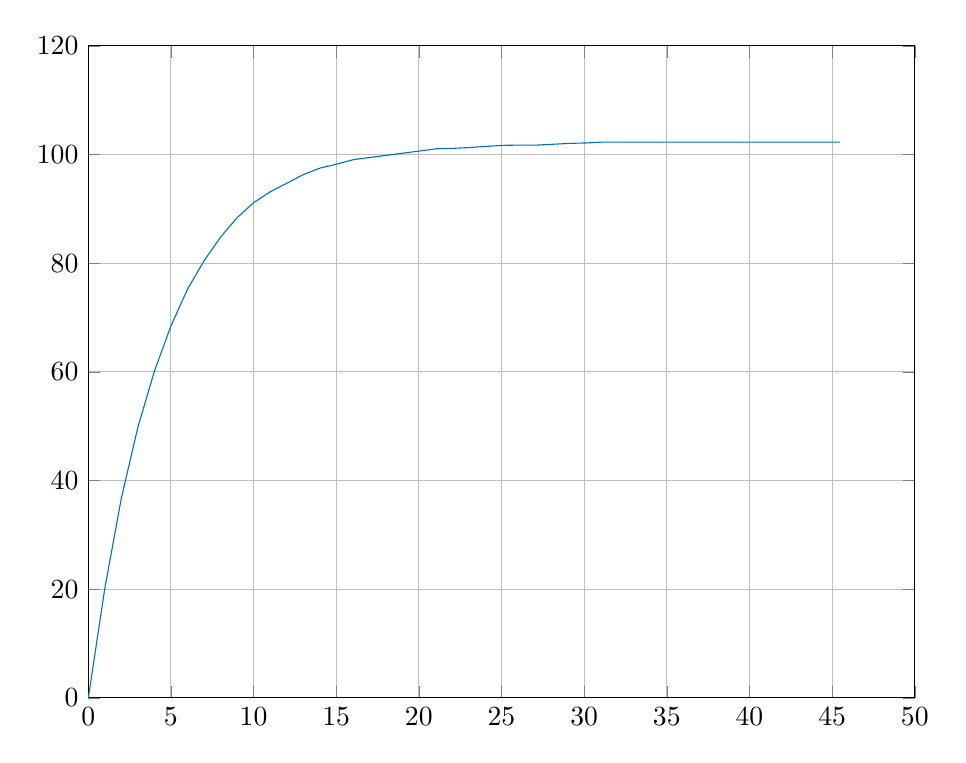
\begin{tikzpicture}

\begin{axis}[%
width=4.133in,
height=3.26in,
at={(0.693in,0.44in)},
scale only axis,
xmin=0,
xmax=50,
xmajorgrids,
ymin=0,
ymax=120,
ymajorgrids,
axis background/.style={fill=white}
]
\addplot [color=mycolor1,solid,forget plot]
  table[row sep=crcr]{%
0	0\\
0.017627004999999	0.178\\
0.0327747189999986	0.47\\
0.0477685379999988	0.792\\
0.0636867769999988	1.118\\
0.0818266279999986	1.468\\
0.0968548159999996	1.782\\
0.111926547	2.09\\
0.127790864	2.4\\
0.143747592	2.722\\
0.159650482999999	3.04\\
0.177841396	3.378\\
0.192911899999998	3.696\\
0.208020343999999	4.016\\
0.223753929	4.334\\
0.239864859999999	4.656\\
0.255788035	4.982\\
0.271866466	5.308\\
0.287787592	5.63\\
0.303792953	5.954\\
0.319799717	6.274\\
0.335788785999998	6.6\\
0.351798507999999	6.924\\
0.367796984999999	7.246\\
0.383892833999999	7.57\\
0.399726994999999	7.892\\
0.417880218999999	8.228\\
0.433032675999999	8.55\\
0.448074034	8.868\\
0.463872045	9.19\\
0.479790275999999	9.51\\
0.495954927999999	9.84\\
0.511977958999999	10.16\\
0.527804439999999	10.482\\
0.543783481999999	10.806\\
0.559864358999999	11.128\\
0.575993435999999	11.458\\
0.591895623	11.78\\
0.607806183999998	12.1\\
0.623805561999999	12.424\\
0.639878685999999	12.744\\
0.655862683999998	13.07\\
0.671809347999999	13.394\\
0.688007375	13.718\\
0.703977030999999	14.04\\
0.719817071999999	14.376\\
0.735789037999999	14.694\\
0.751903521	15.012\\
0.767862266999999	15.336\\
0.78380684	15.656\\
0.799775462999999	15.98\\
0.81574808	16.302\\
0.831793863	16.628\\
0.847800606999999	16.948\\
0.863872895	17.272\\
0.879949246999999	17.61\\
0.896461672999998	17.938\\
0.911939472999999	18.252\\
0.928073790999999	18.574\\
0.944029895	18.89\\
0.959984832999999	19.216\\
0.976055911999999	19.538\\
0.992033660999998	19.864\\
1.012990514	20.23\\
1.025009675	20.48\\
1.040490137	20.728\\
1.055992294	21.004\\
1.071960656	21.266\\
1.088198667	21.522\\
1.104155596	21.794\\
1.11988478	22.054\\
1.13593575	22.312\\
1.151771797	22.578\\
1.167630294	22.836\\
1.185782897	23.108\\
1.201377082	23.386\\
1.216831846	23.646\\
1.232294868	23.908\\
1.248046299	24.166\\
1.263878221	24.43\\
1.279828496	24.692\\
1.295736922	24.958\\
1.311727252	25.22\\
1.327788756	25.488\\
1.343763182	25.754\\
1.359802976	26.028\\
1.375801552	26.29\\
1.39177865	26.554\\
1.407700529	26.816\\
1.423930848	27.08\\
1.440279624	27.352\\
1.456002694	27.614\\
1.471926449	27.874\\
1.488010619	28.14\\
1.503817976	28.404\\
1.519900482	28.668\\
1.535805181	28.932\\
1.552002246	29.196\\
1.56821883	29.472\\
1.583995539	29.738\\
1.599878204	30.01\\
1.615790014	30.264\\
1.631877599	30.53\\
1.647664555	30.788\\
1.665701588	31.064\\
1.680928124	31.326\\
1.696404631	31.59\\
1.71186283	31.852\\
1.730252207	32.126\\
1.745645141	32.402\\
1.761083347	32.658\\
1.776474597	32.918\\
1.79196574	33.182\\
1.807868222	33.442\\
1.823795551	33.708\\
1.839802816	33.972\\
1.855789395	34.236\\
1.871808517	34.508\\
1.887929471	34.772\\
1.903865954	35.048\\
1.919657486	35.306\\
1.935961966	35.566\\
1.952033898	35.84\\
1.968023889	36.112\\
1.983856769	36.37\\
1.999759955	36.628\\
2.015796794	36.876\\
2.031812557	37.092\\
2.047764207	37.292\\
2.063752644	37.49\\
2.079965696	37.694\\
2.095818827	37.902\\
2.112126193	38.114\\
2.127809033	38.33\\
2.143827403	38.534\\
2.15982371	38.742\\
2.175876498	38.954\\
2.191776335	39.162\\
2.207786788	39.372\\
2.22386105	39.58\\
2.239829167	39.792\\
2.255861534	40.002\\
2.271812918	40.208\\
2.287824834	40.416\\
2.303867951	40.628\\
2.319808069	40.836\\
2.335757003	41.046\\
2.351769706	41.252\\
2.367820199	41.464\\
2.383719034	41.672\\
2.399745996	41.882\\
2.415802099	42.1\\
2.431804415	42.308\\
2.447744153	42.512\\
2.463769394	42.722\\
2.479741956	42.93\\
2.495743564	43.138\\
2.511940698	43.348\\
2.527858325	43.558\\
2.543976016	43.768\\
2.559815597	43.974\\
2.575868305	44.184\\
2.591871847	44.394\\
2.608070682	44.602\\
2.624005909	44.814\\
2.640049349	45.022\\
2.655665488	45.232\\
2.673942147	45.454\\
2.689472021	45.664\\
2.704838134	45.868\\
2.720318682	46.074\\
2.735801307	46.28\\
2.751804645	46.486\\
2.767919825	46.71\\
2.783806552	46.916\\
2.799954908	47.12\\
2.815892515	47.328\\
2.831927218	47.534\\
2.847739999	47.742\\
2.864243923	47.952\\
2.879977955	48.172\\
2.895694244	48.378\\
2.911711427	48.584\\
2.927872543	48.792\\
2.943880107	49\\
2.960152786	49.208\\
2.976136849	49.418\\
2.992442385	49.63\\
3.010645236	49.852\\
3.024073413	50.016\\
3.039995715	50.17\\
3.055957568	50.328\\
3.071891633	50.492\\
3.088032265	50.662\\
3.103986055	50.826\\
3.119999544	50.992\\
3.135817002	51.154\\
3.151656771	51.316\\
3.169655073	51.49\\
3.184560306	51.65\\
3.199850563	51.812\\
3.216011025	51.986\\
3.232002044	52.148\\
3.247731998	52.31\\
3.263960171	52.472\\
3.279937487	52.638\\
3.29590332	52.8\\
3.311825067	52.966\\
3.328017257	53.132\\
3.343986025	53.296\\
3.359980577	53.462\\
3.375999619	53.626\\
3.391820693	53.79\\
3.407689629	53.956\\
3.42366058	54.12\\
3.440004937	54.292\\
3.456107988	54.458\\
3.471868399	54.618\\
3.487793105	54.782\\
3.503883728	54.948\\
3.519863356	55.116\\
3.535815948	55.278\\
3.551801023	55.442\\
3.567816813	55.604\\
3.583756631	55.77\\
3.600207591	55.934\\
3.616034661	56.11\\
3.631973083	56.268\\
3.647802512	56.434\\
3.663665581	56.594\\
3.679625737	56.768\\
3.695994628	56.928\\
3.711881169	57.092\\
3.727860845	57.256\\
3.743966872	57.42\\
3.760035076	57.582\\
3.775954432	57.754\\
3.794297178	57.924\\
3.809654195	58.094\\
3.82476268	58.252\\
3.839869516	58.412\\
3.855807023	58.576\\
3.871868883	58.738\\
3.888104941	58.906\\
3.903784654	59.068\\
3.919657818	59.234\\
3.937701482	59.406\\
3.95291856	59.566\\
3.968301958	59.73\\
3.983983911	59.892\\
3.999825184	60.056\\
4.017519282	60.228\\
4.032710384	60.35\\
4.047866862	60.478\\
4.064139198	60.612\\
4.080029619	60.752\\
4.095882935	60.886\\
4.111873057	61.014\\
4.128136433	61.144\\
4.143892278	61.274\\
4.159739011	61.404\\
4.177935996	61.544\\
4.193345052	61.678\\
4.208641668	61.806\\
4.224113879	61.938\\
4.239947172	62.08\\
4.25597298	62.21\\
4.271930102	62.342\\
4.287987125	62.474\\
4.303951243	62.604\\
4.319947318	62.738\\
4.33594442	62.874\\
4.351974207	63.004\\
4.367976556	63.142\\
4.384053314	63.278\\
4.399827501	63.408\\
4.416341439	63.538\\
4.43181896	63.674\\
4.447804054	63.804\\
4.463974977	63.936\\
4.479937368	64.07\\
4.495878271	64.204\\
4.512020782	64.336\\
4.527884096	64.472\\
4.543892205	64.604\\
4.560117343	64.738\\
4.575878175	64.87\\
4.591862339	65.004\\
4.60795167	65.136\\
4.623975423	65.268\\
4.63998543	65.404\\
4.655723423	65.536\\
4.671695315	65.672\\
4.687811757	65.812\\
4.703935277	65.94\\
4.719812847	66.072\\
4.736035157	66.202\\
4.751879723	66.334\\
4.76798453	66.468\\
4.783822211	66.6\\
4.799956619	66.74\\
4.816068272	66.87\\
4.832021379	67.002\\
4.847904669	67.136\\
4.863997323	67.268\\
4.880132879	67.4\\
4.895649057	67.534\\
4.913762656	67.67\\
4.928748145	67.804\\
4.943924162	67.936\\
4.959808103	68.066\\
4.975789906	68.198\\
4.99176524	68.334\\
5.009068286	68.476\\
5.024370002	68.58\\
5.039933467	68.682\\
5.055988474	68.786\\
5.071998062	68.902\\
5.087819251	69.01\\
5.103805213	69.114\\
5.119851335	69.218\\
5.135966847	69.326\\
5.151649607	69.434\\
5.16764885	69.54\\
5.185692803	69.654\\
5.201113096	69.76\\
5.216486093	69.866\\
5.231982492	69.972\\
5.247898811	70.082\\
5.263797546	70.188\\
5.27980209	70.296\\
5.295776747	70.406\\
5.31182054	70.51\\
5.327991732	70.618\\
5.343874794	70.726\\
5.359873114	70.836\\
5.37587304	70.944\\
5.391872199	71.05\\
5.407690814	71.16\\
5.423662849	71.27\\
5.43987021	71.376\\
5.455733015	71.48\\
5.471794601	71.594\\
5.487823922	71.7\\
5.503824307	71.812\\
5.51982593	71.916\\
5.535817074	72.022\\
5.551801493	72.13\\
5.567802253	72.24\\
5.583915624	72.35\\
5.599790274	72.454\\
5.615828665	72.564\\
5.631818301	72.67\\
5.647945694	72.778\\
5.663646814	72.884\\
5.679891156	72.99\\
5.695861745	73.1\\
5.711814472	73.206\\
5.727862319	73.316\\
5.743821266	73.42\\
5.759807609	73.53\\
5.775791551	73.642\\
5.791800621	73.748\\
5.807805982	73.856\\
5.823799376	73.96\\
5.839791256	74.07\\
5.855824616	74.176\\
5.871799659	74.288\\
5.887755623	74.394\\
5.903704049	74.502\\
5.921724081	74.614\\
5.936761629	74.718\\
5.951810318	74.824\\
5.967852728	74.93\\
5.98379203	75.04\\
5.999801205	75.146\\
6.017264463	75.258\\
6.032409405	75.338\\
6.047793604	75.416\\
6.06381671	75.498\\
6.079849469	75.582\\
6.095790399	75.662\\
6.111870364	75.75\\
6.127954634	75.832\\
6.143857899	75.916\\
6.159676503	76\\
6.178057595	76.086\\
6.193509908	76.172\\
6.208640332	76.25\\
6.223923328	76.332\\
6.239998472	76.422\\
6.255798688	76.504\\
6.271888646	76.586\\
6.287788683	76.668\\
6.303821487	76.752\\
6.319868678	76.834\\
6.335758226	76.92\\
6.351808204	77.002\\
6.367935712	77.086\\
6.383771678	77.17\\
6.399881913	77.256\\
6.415683113	77.338\\
6.433990748	77.426\\
6.449409285	77.508\\
6.464666952	77.59\\
6.480081064	77.676\\
6.495982991	77.758\\
6.511820096	77.844\\
6.52779437	77.922\\
6.561458611	78.026\\
6.566951054	78.098\\
6.575775965	78.176\\
6.591698844	78.256\\
6.609903056	78.346\\
6.625018457	78.428\\
6.640392152	78.512\\
6.655669563	78.596\\
6.673841178	78.682\\
6.688906606	78.764\\
6.704260517	78.85\\
6.719812025	78.932\\
6.735893719	79.014\\
6.751819076	79.094\\
6.767860517	79.18\\
6.783908014	79.266\\
6.7997936	79.35\\
6.815864408	79.432\\
6.831863485	79.516\\
6.847906865	79.6\\
6.863861132	79.682\\
6.879676884	79.768\\
6.896006415	79.852\\
6.911657869	79.938\\
6.927860502	80.018\\
6.94369346	80.1\\
6.959823531	80.184\\
6.9758632	80.27\\
6.991885189	80.352\\
7.00948517	80.444\\
7.024426289	80.512\\
7.039677298	80.578\\
7.055689692	80.644\\
7.071722285	80.722\\
7.087716341	80.79\\
7.103810163	80.858\\
7.119807335	80.924\\
7.135860429	80.992\\
7.151679383	81.062\\
7.167643742	81.134\\
7.185934224	81.206\\
7.201095538	81.274\\
7.21640644	81.346\\
7.231757846	81.416\\
7.247865384	81.484\\
7.263864143	81.552\\
7.279708539	81.622\\
7.295882535	81.692\\
7.311827324	81.762\\
7.327747191	81.832\\
7.343857996	81.902\\
7.35978732	81.972\\
7.375788366	82.042\\
7.391945321	82.11\\
7.407687765	82.18\\
7.425965365	82.252\\
7.441202461	82.322\\
7.45642996	82.394\\
7.471824818	82.46\\
7.487877432	82.53\\
7.503882822	82.6\\
7.519744581	82.668\\
7.535691337	82.738\\
7.551893524	82.808\\
7.567887389	82.882\\
7.583888606	82.95\\
7.599816401	83.02\\
7.615863282	83.09\\
7.631853937	83.156\\
7.647931993	83.226\\
7.66549047	83.298\\
7.680518346	83.366\\
7.69611649	83.436\\
7.711876591	83.506\\
7.72787203	83.576\\
7.743948931	83.648\\
7.759749242	83.718\\
7.775828293	83.784\\
7.791858556	83.856\\
7.80771977	83.924\\
7.823765762	83.992\\
7.839742714	84.062\\
7.855719797	84.132\\
7.87172126	84.202\\
7.887887059	84.274\\
7.90375023	84.342\\
7.919874387	84.412\\
7.935851307	84.482\\
7.951780743	84.552\\
7.967936338	84.622\\
7.983877699	84.692\\
7.999872474	84.762\\
8.017289673	84.832\\
8.032245091	84.89\\
8.04763903	84.94\\
8.065696498	84.998\\
8.080668024	85.056\\
8.095876252	85.114\\
8.111870934	85.17\\
8.127870181	85.226\\
8.143972467	85.282\\
8.159678654	85.34\\
8.177706287	85.396\\
8.192922015	85.456\\
8.208198169	85.51\\
8.223801299	85.57\\
8.239818151	85.624\\
8.255660558	85.68\\
8.274159738	85.742\\
8.289633987	85.796\\
8.305104366	85.854\\
8.320541299	85.91\\
8.335964807	85.968\\
8.351868499	86.022\\
8.367887245	86.084\\
8.383698391	86.14\\
8.399640567	86.198\\
8.417764893	86.252\\
8.433303919	86.312\\
8.448830031	86.368\\
8.464404805	86.424\\
8.479893582	86.48\\
8.495911026	86.538\\
8.511791925	86.594\\
8.527852687	86.65\\
8.543787388	86.71\\
8.559786545	86.764\\
8.575815365	86.822\\
8.591805957	86.88\\
8.607862249	86.94\\
8.623720291	86.994\\
8.639911007	87.054\\
8.655672235	87.112\\
8.671764948	87.166\\
8.687892562	87.224\\
8.703952626	87.28\\
8.719695361	87.338\\
8.735950867	87.394\\
8.751786448	87.45\\
8.767853239	87.508\\
8.783810831	87.564\\
8.799793356	87.622\\
8.815821188	87.68\\
8.83178271	87.736\\
8.847822609	87.792\\
8.863706475	87.85\\
8.879804456	87.912\\
8.895902557	87.964\\
8.911782706	88.024\\
8.927698842	88.08\\
8.943768055	88.136\\
8.959796879	88.192\\
8.975795059	88.25\\
8.991776516	88.306\\
9.009183798	88.37\\
9.024356738	88.414\\
9.039791547	88.454\\
9.055750553	88.496\\
9.071819048	88.54\\
9.087806298	88.584\\
9.103760237	88.63\\
9.119860534	88.676\\
9.135748083	88.722\\
9.151731427	88.762\\
9.16764455	88.808\\
9.1837989	88.852\\
9.199793517	88.896\\
9.21593639	88.942\\
9.23182003	88.984\\
9.2479285	89.03\\
9.263788822	89.072\\
9.279958025	89.12\\
9.295662011	89.164\\
9.311772648	89.208\\
9.327785396	89.252\\
9.343896953	89.296\\
9.36174587	89.34\\
9.37686792	89.386\\
9.391936599	89.43\\
9.407782895	89.472\\
9.423824204	89.516\\
9.439745033	89.562\\
9.455852901	89.606\\
9.471818392	89.652\\
9.487779052	89.694\\
9.503896442	89.74\\
9.519679327	89.784\\
9.537731842	89.828\\
9.552990903	89.872\\
9.568209512	89.918\\
9.583787635	89.962\\
9.599762262	90.006\\
9.615849664	90.054\\
9.631664779	90.094\\
9.647854574	90.14\\
9.663722671	90.184\\
9.679672128	90.226\\
9.695786852	90.272\\
9.711790344	90.316\\
9.727860316	90.362\\
9.743805837	90.404\\
9.759822954	90.45\\
9.775941206	90.494\\
9.79177988	90.54\\
9.807783946	90.582\\
9.823803923	90.626\\
9.839762147	90.672\\
9.855791197	90.716\\
9.871864011	90.762\\
9.887853005	90.806\\
9.90364736	90.852\\
9.921648706	90.896\\
9.936677319	90.94\\
9.951642233	90.982\\
9.967677502	91.026\\
9.983782489	91.072\\
9.999776034	91.116\\
10.017032729	91.156\\
10.031978272	91.188\\
10.047690637	91.218\\
10.06577541	91.25\\
10.080814346	91.284\\
10.095871258	91.316\\
10.111786771	91.348\\
10.127786199	91.378\\
10.143779097	91.408\\
10.159640141	91.44\\
10.177696212	91.472\\
10.192853838	91.504\\
10.208131443	91.536\\
10.223802675	91.568\\
10.239674315	91.598\\
10.25586475	91.632\\
10.271851904	91.664\\
10.287802486	91.696\\
10.303807967	91.726\\
10.319863643	91.756\\
10.335894036	91.786\\
10.35167594	91.818\\
10.367813817	91.852\\
10.383893406	91.886\\
10.399952478	91.916\\
10.415702439	91.946\\
10.431788034	91.976\\
10.447799307	92.01\\
10.463866425	92.042\\
10.479969056	92.076\\
10.495809869	92.106\\
10.511784245	92.136\\
10.527786086	92.168\\
10.543734214	92.2\\
10.560073714	92.234\\
10.575998573	92.266\\
10.591904163	92.298\\
10.607980956	92.328\\
10.623763951	92.358\\
10.639788313	92.392\\
10.655690043	92.424\\
10.673977748	92.456\\
10.689360587	92.488\\
10.704531717	92.518\\
10.719792021	92.55\\
10.735798239	92.582\\
10.75186553	92.614\\
10.767775791	92.648\\
10.783775264	92.678\\
10.799749044	92.708\\
10.815782855	92.738\\
10.831717566	92.772\\
10.847758733	92.806\\
10.863861364	92.838\\
10.879660949	92.868\\
10.895823336	92.898\\
10.911650793	92.93\\
10.92980154	92.964\\
10.945560424	92.996\\
10.961214712	93.026\\
10.976697902	93.056\\
10.992021073	93.088\\
11.009933884	93.124\\
11.025040045	93.148\\
11.040313713	93.174\\
11.055786283	93.196\\
11.071773382	93.224\\
11.087742231	93.248\\
11.103751972	93.274\\
11.11972356	93.298\\
11.135746382	93.326\\
11.151727239	93.35\\
11.167700504	93.376\\
11.183758031	93.398\\
11.199829557	93.426\\
11.216047419	93.448\\
11.232014524	93.476\\
11.247744406	93.498\\
11.263763681	93.526\\
11.27981097	93.552\\
11.29579802	93.576\\
11.311791158	93.604\\
11.327771552	93.626\\
11.343754788	93.654\\
11.359972802	93.678\\
11.375888118	93.706\\
11.392157899	93.728\\
11.407860489	93.756\\
11.42365893	93.778\\
11.441916249	93.806\\
11.457588499	93.83\\
11.473253783	93.856\\
11.488803536	93.886\\
11.504431502	93.906\\
11.519934064	93.934\\
11.536288165	93.956\\
11.551979189	93.984\\
11.567796525	94.006\\
11.583773792	94.036\\
11.599772218	94.058\\
11.615850008	94.086\\
11.631792206	94.11\\
11.647954717	94.136\\
11.663663578	94.16\\
11.681747497	94.186\\
11.697206305	94.214\\
11.712599745	94.236\\
11.728058099	94.266\\
11.743995995	94.286\\
11.759795626	94.316\\
11.775782826	94.336\\
11.791787054	94.366\\
11.807740087	94.388\\
11.82377295	94.416\\
11.83976647	94.438\\
11.855942387	94.466\\
11.871882731	94.488\\
11.887826409	94.516\\
11.903721295	94.538\\
11.922163025	94.566\\
11.937720696	94.594\\
11.953041426	94.616\\
11.968370636	94.644\\
11.983893938	94.668\\
11.999905004	94.694\\
12.017284458	94.722\\
12.032417538	94.746\\
12.047797457	94.77\\
12.063989406	94.796\\
12.079796247	94.82\\
12.095686649	94.846\\
12.112067325	94.87\\
12.127865446	94.896\\
12.143816259	94.922\\
12.159651027	94.946\\
12.177698274	94.974\\
12.192953867	94.996\\
12.208369859	95.024\\
12.223922395	95.046\\
12.239957659	95.076\\
12.255889102	95.098\\
12.271873441	95.126\\
12.287864675	95.148\\
12.30380106	95.176\\
12.319820087	95.198\\
12.336503449	95.226\\
12.351913397	95.252\\
12.367694297	95.276\\
12.383798895	95.304\\
12.399808599	95.326\\
12.415688548	95.354\\
12.43188638	95.376\\
12.44774749	95.404\\
12.463642034	95.428\\
12.479716257	95.458\\
12.495730589	95.478\\
12.511766939	95.506\\
12.527956128	95.528\\
12.543955981	95.556\\
12.559794459	95.582\\
12.575722483	95.606\\
12.592062439	95.634\\
12.607760823	95.656\\
12.623762671	95.684\\
12.639766226	95.706\\
12.655875988	95.736\\
12.671647968	95.758\\
12.689894019	95.786\\
12.705433091	95.81\\
12.721022436	95.836\\
12.736595895	95.86\\
12.751984769	95.886\\
12.768229963	95.912\\
12.784077096	95.936\\
12.800274607	95.964\\
12.815902278	95.986\\
12.831804952	96.014\\
12.847796557	96.036\\
12.863970004	96.064\\
12.885462958	96.09\\
12.897481368	96.116\\
12.912772037	96.142\\
12.928278493	96.166\\
12.943775676	96.188\\
12.959911936	96.216\\
12.975750846	96.238\\
12.991781669	96.266\\
13.01254802	96.296\\
13.024416124	96.308\\
13.039827555	96.328\\
13.055822899	96.348\\
13.071781674	96.368\\
13.09010038	96.388\\
13.10511796	96.406\\
13.120279834	96.426\\
13.135774828	96.446\\
13.151665986	96.462\\
13.169703295	96.48\\
13.184865433	96.498\\
13.200007553	96.52\\
13.216155553	96.538\\
13.231799509	96.558\\
13.247914334	96.578\\
13.2637422	96.596\\
13.2797809	96.616\\
13.295781454	96.636\\
13.314162745	96.654\\
13.329294355	96.67\\
13.344380055	96.688\\
13.359871988	96.708\\
13.375699269	96.728\\
13.391810906	96.748\\
13.40772616	96.768\\
13.423987777	96.788\\
13.439753987	96.806\\
13.455884569	96.826\\
13.471795957	96.844\\
13.487891437	96.862\\
13.503819744	96.88\\
13.519933562	96.9\\
13.5358178	96.918\\
13.551805945	96.938\\
13.567884657	96.958\\
13.583927984	96.978\\
13.599823909	96.996\\
13.615738683	97.016\\
13.631861933	97.036\\
13.647887573	97.05\\
13.663681336	97.068\\
13.679678923	97.088\\
13.697775157	97.108\\
13.712993406	97.128\\
13.72813961	97.148\\
13.74389068	97.168\\
13.759725303	97.186\\
13.775867666	97.206\\
13.79185465	97.226\\
13.807805794	97.242\\
13.823863228	97.258\\
13.84001179	97.278\\
13.855669229	97.298\\
13.871820539	97.318\\
13.887863199	97.338\\
13.903926136	97.358\\
13.919693996	97.376\\
13.935866018	97.396\\
13.951712619	97.416\\
13.967859033	97.432\\
13.983821544	97.45\\
13.99998371	97.468\\
14.017401031	97.488\\
14.032850492	97.498\\
14.048055229	97.512\\
14.06389067	97.528\\
14.079861388	97.538\\
14.095806004	97.548\\
14.111874146	97.562\\
14.127864332	97.578\\
14.143658792	97.588\\
14.161737314	97.598\\
14.176606747	97.614\\
14.191639854	97.628\\
14.209825548	97.638\\
14.225007175	97.65\\
14.240200642	97.668\\
14.255777753	97.678\\
14.271952699	97.688\\
14.287703853	97.702\\
14.303878313	97.718\\
14.319879389	97.728\\
14.335796235	97.738\\
14.351780679	97.752\\
14.367769638	97.768\\
14.383812038	97.778\\
14.400056211	97.788\\
14.415679017	97.804\\
14.431652417	97.818\\
14.447810581	97.828\\
14.549835343	97.854\\
14.567883932	97.872\\
14.583028783	97.882\\
14.598227052	97.892\\
14.613992099	97.906\\
14.630003103	97.922\\
14.64597791	97.932\\
14.66197217	97.942\\
14.67782766	97.956\\
14.695988156	97.972\\
14.711244948	97.982\\
14.72647896	97.994\\
14.742313078	98.008\\
14.758250536	98.022\\
14.774059151	98.032\\
14.790003113	98.046\\
14.806165585	98.06\\
14.822019563	98.072\\
14.838105371	98.082\\
14.854005462	98.096\\
14.870046942	98.112\\
14.88605715	98.122\\
14.901879986	98.134\\
14.920148164	98.15\\
14.935448993	98.162\\
14.950779369	98.172\\
14.966098463	98.186\\
14.981994657	98.2\\
14.998048222	98.212\\
15.015722995	98.222\\
15.030955506	98.236\\
15.0461657	98.252\\
15.062008338	98.262\\
15.077963245	98.272\\
15.093960327	98.288\\
15.110067945	98.302\\
15.125987216	98.312\\
15.142027732	98.324\\
15.158057018	98.338\\
15.173976915	98.352\\
15.189969592	98.362\\
15.205974628	98.376\\
15.222033721	98.39\\
15.237839046	98.402\\
15.254080174	98.412\\
15.270029809	98.426\\
15.285944329	98.442\\
15.302009686	98.452\\
15.317968277	98.462\\
15.334083923	98.476\\
15.350038875	98.492\\
15.365915945	98.502\\
15.381981483	98.514\\
15.397930691	98.53\\
15.413814783	98.542\\
15.430014931	98.552\\
15.445987703	98.566\\
15.462046406	98.58\\
15.478054524	98.592\\
15.493962092	98.602\\
15.509984066	98.616\\
15.525987688	98.632\\
15.541971942	98.642\\
15.558014342	98.654\\
15.574018189	98.666\\
15.589902778	98.682\\
15.605971161	98.692\\
15.622028971	98.704\\
15.637985306	98.72\\
15.654193321	98.732\\
15.670030446	98.744\\
15.686000978	98.756\\
15.701995415	98.77\\
15.718020516	98.782\\
15.733943751	98.792\\
15.749943845	98.808\\
15.765963985	98.822\\
15.782092279	98.832\\
15.797959375	98.842\\
15.813988718	98.856\\
15.830073479	98.872\\
15.845985884	98.882\\
15.861895561	98.896\\
15.877974462	98.91\\
15.893959627	98.922\\
15.909872714	98.932\\
15.926041223	98.946\\
15.941945081	98.962\\
15.957984585	98.972\\
15.974038701	98.984\\
15.989988527	98.996\\
16.008685309	99.012\\
16.023937795	99.02\\
16.039299975	99.03\\
16.054581055	99.046\\
16.06997232	99.056\\
16.086109109	99.066\\
16.102019645	99.074\\
16.117919021	99.084\\
16.13403094	99.092\\
16.150088263	99.094\\
16.165937074	99.104\\
16.184047898	99.108\\
16.199447043	99.114\\
16.214637436	99.122\\
16.230096627	99.124\\
16.246064263	99.134\\
16.262199208	99.142\\
16.277968704	99.144\\
16.293963256	99.154\\
16.309968832	99.16\\
16.325961746	99.164\\
16.341966906	99.174\\
16.357952483	99.174\\
16.373974752	99.184\\
16.390075409	99.192\\
16.405939167	99.194\\
16.421937901	99.204\\
16.437899418	99.21\\
16.453866954	99.214\\
16.469993829	99.224\\
16.485997918	99.23\\
16.501991823	99.234\\
16.51799338	99.244\\
16.533955448	99.244\\
16.549906676	99.254\\
16.566134217	99.262\\
16.582160875	99.264\\
16.598096614	99.274\\
16.613988193	99.28\\
16.630037323	99.284\\
16.645985074	99.294\\
16.661840539	99.296\\
16.679970289	99.304\\
16.695042607	99.314\\
16.710292201	99.314\\
16.725973232	99.324\\
16.74209833	99.332\\
16.757955906	99.334\\
16.774004881	99.344\\
16.79017237	99.35\\
16.80613542	99.354\\
16.822120615	99.364\\
16.837949952	99.366\\
16.854034348	99.374\\
16.870082266	99.384\\
16.886018279	99.384\\
16.902144429	99.394\\
16.918020177	99.402\\
16.933977524	99.404\\
16.950000057	99.414\\
16.965987094	99.42\\
16.981977885	99.424\\
16.998000683	99.434\\
17.015391868	99.436\\
17.030454143	99.444\\
17.04596982	99.452\\
17.061964066	99.454\\
17.077945328	99.464\\
17.09398425	99.474\\
17.109964299	99.474\\
17.126004023	99.484\\
17.142068874	99.49\\
17.158040293	99.494\\
17.17403095	99.504\\
17.190065513	99.504\\
17.206143514	99.514\\
17.222087416	99.522\\
17.238095799	99.524\\
17.254090716	99.534\\
17.270008459	99.54\\
17.28611973	99.544\\
17.302142566	99.554\\
17.318139678	99.556\\
17.334151163	99.564\\
17.350127293	99.574\\
17.365938525	99.574\\
17.381904401	99.584\\
17.400379986	99.592\\
17.415299264	99.594\\
17.430387247	99.604\\
17.446147817	99.61\\
17.462092222	99.614\\
17.4782019	99.624\\
17.493970848	99.626\\
17.50986969	99.634\\
17.526107337	99.642\\
17.541999823	99.644\\
17.557967356	99.654\\
17.574030976	99.662\\
17.590012639	99.664\\
17.605950663	99.674\\
17.621969539	99.68\\
17.637941219	99.684\\
17.654074415	99.694\\
17.6698351	99.696\\
17.687979974	99.704\\
17.703261456	99.712\\
17.718304107	99.714\\
17.733927875	99.724\\
17.749959904	99.73\\
17.765940179	99.734\\
17.781924097	99.744\\
17.797913652	99.746\\
17.814003249	99.754\\
17.829902438	99.764\\
17.846086212	99.764\\
17.862094533	99.774\\
17.878132252	99.782\\
17.894149801	99.784\\
17.909994519	99.794\\
17.926020474	99.8\\
17.942101419	99.804\\
17.958068077	99.814\\
17.97404948	99.818\\
17.990057446	99.824\\
18.008500996	99.834\\
18.023565164	99.834\\
18.038760476	99.844\\
18.053959761	99.852\\
18.069906127	99.854\\
18.085848492	99.864\\
18.10195646	99.872\\
18.118017002	99.874\\
18.134006156	99.884\\
18.14999943	99.886\\
18.165845217	99.894\\
18.182095405	99.904\\
18.198230751	99.904\\
18.213866039	99.914\\
18.229867737	99.922\\
18.245857485	99.924\\
18.261911033	99.934\\
18.278030547	99.94\\
18.294004462	99.944\\
18.309912172	99.954\\
18.325919323	99.954\\
18.341995269	99.964\\
18.35794546	99.972\\
18.373969613	99.974\\
18.390000723	99.984\\
18.405971824	99.992\\
18.422006246	99.994\\
18.437909932	100.004\\
18.45399883	100.008\\
18.469970824	100.014\\
18.48599559	100.024\\
18.501907135	100.024\\
18.518041422	100.034\\
18.533999076	100.042\\
18.550062476	100.044\\
18.568264718	100.054\\
18.583290984	100.062\\
18.598352492	100.064\\
18.613993172	100.074\\
18.629979921	100.076\\
18.645961674	100.084\\
18.661829833	100.094\\
18.680035299	100.096\\
18.695102175	100.104\\
18.710207522	100.112\\
18.726177458	100.114\\
18.742354418	100.124\\
18.757942469	100.13\\
18.774014641	100.134\\
18.789964907	100.144\\
18.805912398	100.146\\
18.821954146	100.154\\
18.837950292	100.164\\
18.854001226	100.164\\
18.869999997	100.174\\
18.885966946	100.182\\
18.90196255	100.184\\
18.917861052	100.194\\
18.935822449	100.2\\
18.950638963	100.204\\
18.965781292	100.214\\
18.982110432	100.214\\
18.998258685	100.224\\
19.015808096	100.232\\
19.031137179	100.234\\
19.046655657	100.244\\
19.062099346	100.252\\
19.078143745	100.254\\
19.093974721	100.264\\
19.110150534	100.272\\
19.126057021	100.274\\
19.142351367	100.284\\
19.15809924	100.284\\
19.173818747	100.294\\
19.189969945	100.302\\
19.206114932	100.304\\
19.22197526	100.314\\
19.237951369	100.32\\
19.253970061	100.324\\
19.270017728	100.334\\
19.286039886	100.336\\
19.302006463	100.344\\
19.318039986	100.354\\
19.333990572	100.354\\
19.349976043	100.364\\
19.365969718	100.372\\
19.381996533	100.374\\
19.397968013	100.384\\
19.413901465	100.39\\
19.430006122	100.394\\
19.44636627	100.404\\
19.462151547	100.406\\
19.478012764	100.414\\
19.494153307	100.424\\
19.510145147	100.424\\
19.525851562	100.434\\
19.54212968	100.442\\
19.558217483	100.444\\
19.574136854	100.454\\
19.590149402	100.46\\
19.605923827	100.464\\
19.624143367	100.474\\
19.639201151	100.476\\
19.654274541	100.484\\
19.669920007	100.492\\
19.6880254	100.494\\
19.703131139	100.504\\
19.718182009	100.512\\
19.733913939	100.514\\
19.75259865	100.524\\
19.768183303	100.528\\
19.783572053	100.534\\
19.799139657	100.544\\
19.814625968	100.544\\
19.830057344	100.554\\
19.846008261	100.562\\
19.862075077	100.564\\
19.87801487	100.574\\
19.893969892	100.58\\
19.909856561	100.584\\
19.927896709	100.594\\
19.943067886	100.598\\
19.958254092	100.604\\
19.974178504	100.614\\
19.990041211	100.614\\
20.008710191	100.624\\
20.023786188	100.632\\
20.039136428	100.634\\
20.054206112	100.644\\
20.069911308	100.65\\
20.085890881	100.654\\
20.101978188	100.664\\
20.117907526	100.668\\
20.133983513	100.674\\
20.149888292	100.682\\
20.165965836	100.684\\
20.181865227	100.694\\
20.197906423	100.702\\
20.214000762	100.704\\
20.230045588	100.714\\
20.246017869	100.72\\
20.261894291	100.724\\
20.278094385	100.734\\
20.294031558	100.734\\
20.310051108	100.744\\
20.325982734	100.752\\
20.341990245	100.754\\
20.35806324	100.764\\
20.373930423	100.772\\
20.390024334	100.774\\
20.406069486	100.784\\
20.422005821	100.79\\
20.438005038	100.794\\
20.453990354	100.804\\
20.469985883	100.804\\
20.485855899	100.814\\
20.501965078	100.824\\
20.518022548	100.824\\
20.533998131	100.834\\
20.550138038	100.84\\
20.565919362	100.844\\
20.581997572	100.854\\
20.597998347	100.856\\
20.613998242	100.864\\
20.629996176	100.874\\
20.645976891	100.874\\
20.66183582	100.884\\
20.679901165	100.892\\
20.69485835	100.894\\
20.710065534	100.904\\
20.725814183	100.91\\
20.741958229	100.914\\
20.757995682	100.924\\
20.77400388	100.928\\
20.789970152	100.934\\
20.805860908	100.944\\
20.821985973	100.944\\
20.838030286	100.954\\
20.854034467	100.962\\
20.869979281	100.964\\
20.885994151	100.974\\
20.902059824	100.98\\
20.917974412	100.984\\
20.93411137	100.994\\
20.950076019	100.994\\
20.966008574	101.004\\
20.982002053	101.012\\
20.99798134	101.014\\
21.015280377	101.024\\
21.030340307	101.032\\
21.045867314	101.034\\
21.062044499	101.044\\
21.0779569	101.048\\
21.093965629	101.054\\
21.109975109	101.056\\
21.126032133	101.056\\
21.141992186	101.058\\
21.158072843	101.06\\
21.173953539	101.06\\
21.189840249	101.062\\
21.205982685	101.064\\
21.221989009	101.064\\
21.237925664	101.066\\
21.253992806	101.066\\
21.270012735	101.068\\
21.285955324	101.07\\
21.30195832	101.07\\
21.318057649	101.072\\
21.334068011	101.074\\
21.349841656	101.074\\
21.3681961	101.076\\
21.383452675	101.078\\
21.398792258	101.078\\
21.413842567	101.08\\
21.431881907	101.082\\
21.447120497	101.082\\
21.462173096	101.084\\
21.477987946	101.084\\
21.493970664	101.086\\
21.509785736	101.088\\
21.525805994	101.088\\
21.541812183	101.09\\
21.557847458	101.092\\
21.574015833	101.092\\
21.589993462	101.094\\
21.605940295	101.094\\
21.621986629	101.096\\
21.637964373	101.098\\
21.654028412	101.098\\
21.669917721	101.1\\
21.685960281	101.102\\
21.702003267	101.102\\
21.718056116	101.104\\
21.734039232	101.106\\
21.749953862	101.106\\
21.765856111	101.108\\
21.781957784	101.108\\
21.797909809	101.11\\
21.813964076	101.112\\
21.830002262	101.112\\
21.845939624	101.114\\
21.861940685	101.116\\
21.878178528	101.116\\
21.894189367	101.118\\
21.90996144	101.12\\
21.925829928	101.12\\
21.944078905	101.122\\
21.959422342	101.122\\
21.974873428	101.124\\
21.990389389	101.126\\
22.00950892	101.126\\
22.021926764	101.126\\
22.04018348	101.126\\
22.055329988	101.126\\
22.070332851	101.126\\
22.086130933	101.126\\
22.101961057	101.126\\
22.117941344	101.13\\
22.133967159	101.134\\
22.149963124	101.134\\
22.165836722	101.138\\
22.183917149	101.142\\
22.199138082	101.142\\
22.214419394	101.144\\
22.229953412	101.148\\
22.245998332	101.15\\
22.261953535	101.152\\
22.277974296	101.156\\
22.293967986	101.158\\
22.309994309	101.158\\
22.326128483	101.164\\
22.342172236	101.166\\
22.358185655	101.166\\
22.374258449	101.172\\
22.390111976	101.174\\
22.406047254	101.174\\
22.421835463	101.178\\
22.439917654	101.182\\
22.454915332	101.182\\
22.470366095	101.186\\
22.485972971	101.19\\
22.501978648	101.19\\
22.518065067	101.194\\
22.53412175	101.196\\
22.550092187	101.198\\
22.566144725	101.2\\
22.582119752	101.204\\
22.598150331	101.206\\
22.614104606	101.208\\
22.630113696	101.212\\
22.64606504	101.214\\
22.662109509	101.214\\
22.677829424	101.22\\
22.695838741	101.222\\
22.710936981	101.222\\
22.726508434	101.226\\
22.742163898	101.23\\
22.758095942	101.23\\
22.774101655	101.234\\
22.790153697	101.238\\
22.806042912	101.238\\
22.82210108	101.242\\
22.838149333	101.246\\
22.854155898	101.246\\
22.870005575	101.248\\
22.888615916	101.252\\
22.904163707	101.254\\
22.919953994	101.256\\
22.935306033	101.26\\
22.950476469	101.262\\
22.966030687	101.262\\
22.981959486	101.268\\
22.997959379	101.27\\
23.015434204	101.27\\
23.03066269	101.278\\
23.045980072	101.28\\
23.062005354	101.28\\
23.077954362	101.286\\
23.093922223	101.29\\
23.110017774	101.29\\
23.12601888	101.296\\
23.141975175	101.3\\
23.157860699	101.3\\
23.173906994	101.306\\
23.189991009	101.308\\
23.206018119	101.31\\
23.221962918	101.314\\
23.238063439	101.318\\
23.253957143	101.32\\
23.269989094	101.322\\
23.286294059	101.328\\
23.302125476	101.33\\
23.318132656	101.33\\
23.334144868	101.338\\
23.350150334	101.34\\
23.366167327	101.34\\
23.382130608	101.348\\
23.397973581	101.35\\
23.413870656	101.35\\
23.429991138	101.356\\
23.445984229	101.36\\
23.462060655	101.36\\
23.477971812	101.366\\
23.493814715	101.37\\
23.510027657	101.37\\
23.526093861	101.374\\
23.542008549	101.378\\
23.558237995	101.38\\
23.574150927	101.382\\
23.590303447	101.388\\
23.606307861	101.39\\
23.62204964	101.39\\
23.63795933	101.398\\
23.654030961	101.4\\
23.669867623	101.4\\
23.687955235	101.408\\
23.702832025	101.41\\
23.717823661	101.41\\
23.735877231	101.416\\
23.751042424	101.42\\
23.766371617	101.42\\
23.781989215	101.426\\
23.798125872	101.43\\
23.814042813	101.43\\
23.82999572	101.436\\
23.846075773	101.438\\
23.862178723	101.44\\
23.877992626	101.444\\
23.893926324	101.448\\
23.912274699	101.45\\
23.927273342	101.454\\
23.942150594	101.458\\
23.958241564	101.46\\
23.974143546	101.46\\
23.99018328	101.468\\
24.00882427	101.47\\
24.021996069	101.47\\
24.037985745	101.478\\
24.054141427	101.48\\
24.07015233	101.48\\
24.086139861	101.486\\
24.102060826	101.49\\
24.118056555	101.49\\
24.134039496	101.496\\
24.149976061	101.5\\
24.165824411	101.5\\
24.183897216	101.504\\
24.199162163	101.508\\
24.214470152	101.51\\
24.229936006	101.512\\
24.24597126	101.518\\
24.262008849	101.52\\
24.278003606	101.52\\
24.29399048	101.528\\
24.30998886	101.53\\
24.325939177	101.53\\
24.341970888	101.538\\
24.357978494	101.54\\
24.373945794	101.54\\
24.390006856	101.546\\
24.406174199	101.55\\
24.423597158	101.55\\
24.438593907	101.556\\
24.454275796	101.56\\
24.470400782	101.56\\
24.486261537	101.566\\
24.501878678	101.57\\
24.518134693	101.57\\
24.534146301	101.574\\
24.549976292	101.578\\
24.568282425	101.58\\
24.583750459	101.584\\
24.599238659	101.588\\
24.614642705	101.59\\
24.630173366	101.59\\
24.646015703	101.598\\
24.662028506	101.6\\
24.677836795	101.6\\
24.6941934	101.606\\
24.7102898	101.61\\
24.72609029	101.61\\
24.741981628	101.616\\
24.75795886	101.62\\
24.774110673	101.62\\
24.789983544	101.626\\
24.805951435	101.63\\
24.822101464	101.63\\
24.837990216	101.634\\
24.853951563	101.638\\
24.869959675	101.64\\
24.885926825	101.642\\
24.901952703	101.648\\
24.917888371	101.65\\
24.933961511	101.65\\
24.950143271	101.658\\
24.966136189	101.66\\
24.982058863	101.66\\
24.998100582	101.668\\
25.015726912	101.67\\
25.031227206	101.67\\
25.046564294	101.676\\
25.062210537	101.68\\
25.078146009	101.68\\
25.094094021	101.684\\
25.110139012	101.684\\
25.125984792	101.684\\
25.142123309	101.686\\
25.158092774	101.686\\
25.173878966	101.686\\
25.191934569	101.688\\
25.207279493	101.688\\
25.222658502	101.688\\
25.238100056	101.688\\
25.25410012	101.69\\
25.269977706	101.69\\
25.286054575	101.69\\
25.301943803	101.692\\
25.317981367	101.692\\
25.334009234	101.692\\
25.349971177	101.694\\
25.366031117	101.694\\
25.382129388	101.694\\
25.397950653	101.696\\
25.413946029	101.696\\
25.429963384	101.696\\
25.445931732	101.698\\
25.462031643	101.698\\
25.478143765	101.698\\
25.493983977	101.7\\
25.509956394	101.7\\
25.525956864	101.7\\
25.544271731	101.702\\
25.559780267	101.702\\
25.575209112	101.702\\
25.590785637	101.702\\
25.606215089	101.704\\
25.622123666	101.704\\
25.638233995	101.704\\
25.654325982	101.706\\
25.669878516	101.706\\
25.687939182	101.706\\
25.703350162	101.708\\
25.71910206	101.708\\
25.734660405	101.708\\
25.750114066	101.71\\
25.766200085	101.71\\
25.782254781	101.71\\
25.798597118	101.712\\
25.814206421	101.712\\
25.830422906	101.712\\
25.846613086	101.714\\
25.862033245	101.714\\
25.877858309	101.714\\
25.893980339	101.714\\
25.909960155	101.716\\
25.926957206	101.716\\
25.942208311	101.716\\
25.958142663	101.718\\
25.9741329	101.718\\
25.990106016	101.718\\
26.008723096	101.72\\
26.023984762	101.72\\
26.03907901	101.72\\
26.054210411	101.72\\
26.069973258	101.72\\
26.085983395	101.72\\
26.101992023	101.72\\
26.118098549	101.72\\
26.13402451	101.72\\
26.150145017	101.72\\
26.166202315	101.72\\
26.181926588	101.72\\
26.197825344	101.72\\
26.213968774	101.72\\
26.230007942	101.72\\
26.2462218	101.72\\
26.26197075	101.72\\
26.27800855	101.72\\
26.29399546	101.72\\
26.309973514	101.72\\
26.325949393	101.72\\
26.341985309	101.72\\
26.357988565	101.72\\
26.374014433	101.72\\
26.389953353	101.72\\
26.406062339	101.72\\
26.421928828	101.72\\
26.438002213	101.72\\
26.454017871	101.72\\
26.469965987	101.72\\
26.485967785	101.72\\
26.502053418	101.72\\
26.518007283	101.72\\
26.534274336	101.72\\
26.550272431	101.72\\
26.566023226	101.72\\
26.58208961	101.72\\
26.59801713	101.72\\
26.61387508	101.72\\
26.629859495	101.72\\
26.646118091	101.72\\
26.661982833	101.72\\
26.677845798	101.72\\
26.694011887	101.72\\
26.710089602	101.72\\
26.726028053	101.72\\
26.742071399	101.72\\
26.758115558	101.72\\
26.774078338	101.72\\
26.790009521	101.72\\
26.82420186	101.72\\
26.840055797	101.72\\
26.856138485	101.72\\
26.872154041	101.72\\
26.888128345	101.72\\
26.904291859	101.72\\
26.920152485	101.72\\
26.936261105	101.72\\
26.952249521	101.72\\
26.968189533	101.72\\
26.984202402	101.72\\
27.000239575	101.72\\
27.017875249	101.72\\
27.033201552	101.72\\
27.04847035	101.72\\
27.064208636	101.72\\
27.080181323	101.72\\
27.09619155	101.72\\
27.112169985	101.722\\
27.128163655	101.726\\
27.144193793	101.726\\
27.160291088	101.73\\
27.176287835	101.734\\
27.19224899	101.734\\
27.208237713	101.736\\
27.224193206	101.742\\
27.240231931	101.742\\
27.256230929	101.744\\
27.272256267	101.748\\
27.288339309	101.75\\
27.304205784	101.75\\
27.320185964	101.756\\
27.336048126	101.758\\
27.354413593	101.758\\
27.369506422	101.762\\
27.384786671	101.766\\
27.400357317	101.766\\
27.416054365	101.77\\
27.432146024	101.774\\
27.44829574	101.774\\
27.464257377	101.778\\
27.48018644	101.782\\
27.49638315	101.782\\
27.512384347	101.786\\
27.528245291	101.79\\
27.54429174	101.79\\
27.560181685	101.792\\
27.576267849	101.796\\
27.604166083	101.798\\
27.609590072	101.798\\
27.624652567	101.804\\
27.640104876	101.806\\
27.656218918	101.806\\
27.672144122	101.812\\
27.690239127	101.814\\
27.705572301	101.814\\
27.720663371	101.818\\
27.736222189	101.822\\
27.752204805	101.822\\
27.7682205	101.826\\
27.784231253	101.83\\
27.800232776	101.83\\
27.816277561	101.834\\
27.832228735	101.838\\
27.848192938	101.838\\
27.864220409	101.84\\
27.88022145	101.846\\
27.896196779	101.846\\
27.912416578	101.848\\
27.928130516	101.852\\
27.944363483	101.854\\
27.960354396	101.854\\
27.976266141	101.86\\
27.992354991	101.862\\
28.010317739	101.862\\
28.025570523	101.868\\
28.040776608	101.87\\
28.056204647	101.87\\
28.072256814	101.874\\
28.088227075	101.878\\
28.10417686	101.878\\
28.120219426	101.882\\
28.136218518	101.886\\
28.152204079	101.886\\
28.1681	101.89\\
28.186075815	101.894\\
28.201494755	101.894\\
28.217019843	101.896\\
28.232499018	101.9\\
28.248598692	101.902\\
28.264349226	101.902\\
28.280216946	101.908\\
28.296199761	101.91\\
28.312224711	101.91\\
28.32829308	101.916\\
28.344370981	101.918\\
28.360170347	101.918\\
28.376183754	101.922\\
28.392159128	101.926\\
28.408213851	101.926\\
28.424047027	101.93\\
28.442152299	101.934\\
28.457503254	101.934\\
28.472837234	101.938\\
28.48827315	101.942\\
28.504353942	101.942\\
28.520258024	101.944\\
28.536148866	101.95\\
28.552044834	101.95\\
28.570327178	101.952\\
28.585875113	101.956\\
28.601378623	101.958\\
28.616782657	101.958\\
28.632228728	101.964\\
28.648216647	101.966\\
28.664133734	101.966\\
28.682233113	101.972\\
28.6976252	101.974\\
28.713258265	101.974\\
28.728491445	101.978\\
28.744362362	101.982\\
28.760403564	101.982\\
28.776390283	101.986\\
28.792429702	101.99\\
28.808384142	101.99\\
28.824460213	101.992\\
28.840357625	101.998\\
28.856485799	101.998\\
28.872313258	102\\
28.888374846	102.004\\
28.904365043	102.006\\
28.920084053	102.006\\
28.938521498	102.012\\
28.953727864	102.014\\
28.969131518	102.014\\
28.984528059	102.02\\
29.000462282	102.022\\
29.018208026	102.022\\
29.033643441	102.026\\
29.049020729	102.03\\
29.064242225	102.032\\
29.080293536	102.036\\
29.096202498	102.04\\
29.112214244	102.042\\
29.128131414	102.044\\
29.14423229	102.044\\
29.160200101	102.046\\
29.176175523	102.048\\
29.192215018	102.048\\
29.208229523	102.05\\
29.224205196	102.052\\
29.240204173	102.052\\
29.256198795	102.052\\
29.27229523	102.054\\
29.288231046	102.056\\
29.304236387	102.056\\
29.320216422	102.058\\
29.336256731	102.06\\
29.352207138	102.06\\
29.368156733	102.062\\
29.384198641	102.064\\
29.402505526	102.064\\
29.417443465	102.066\\
29.433198383	102.068\\
29.448257297	102.068\\
29.464234403	102.07\\
29.480087665	102.072\\
29.496189775	102.072\\
29.51219472	102.074\\
29.528189673	102.076\\
29.544219038	102.076\\
29.560237254	102.078\\
29.576259233	102.078\\
29.592225284	102.08\\
29.6082982	102.08\\
29.624230335	102.082\\
29.640214467	102.084\\
29.65621828	102.084\\
29.6730843	102.086\\
29.688333183	102.088\\
29.704187607	102.088\\
29.720048214	102.09\\
29.736299499	102.092\\
29.752199897	102.092\\
29.768192724	102.094\\
29.784194232	102.096\\
29.800114535	102.096\\
29.816213529	102.098\\
29.832289671	102.1\\
29.848216564	102.1\\
29.864354526	102.102\\
29.880330591	102.104\\
29.896234412	102.104\\
29.912230755	102.104\\
29.928058857	102.106\\
29.946212079	102.108\\
29.961643069	102.108\\
29.977166413	102.11\\
29.992449789	102.112\\
30.008159032	102.112\\
30.024243039	102.112\\
30.040212875	102.114\\
30.056232915	102.114\\
30.072243627	102.114\\
30.088326549	102.116\\
30.104342103	102.116\\
30.120430943	102.116\\
30.136222901	102.122\\
30.152216551	102.124\\
30.168064293	102.124\\
30.186153376	102.128\\
30.20160143	102.132\\
30.216682272	102.132\\
30.232256215	102.132\\
30.248197015	102.14\\
30.264314886	102.14\\
30.280252595	102.14\\
30.296202996	102.148\\
30.312218576	102.148\\
30.328223	102.148\\
30.344147777	102.156\\
30.360182015	102.156\\
30.376216878	102.156\\
30.392194045	102.164\\
30.410390881	102.164\\
30.425640095	102.164\\
30.440690898	102.17\\
30.456127029	102.172\\
30.47252498	102.172\\
30.488416453	102.176\\
30.504709005	102.18\\
30.520339169	102.18\\
30.536450036	102.184\\
30.552473358	102.188\\
30.568295379	102.188\\
30.58682566	102.188\\
30.601915001	102.196\\
30.616976093	102.196\\
30.632183582	102.196\\
30.648404461	102.204\\
30.666784267	102.204\\
30.680060454	102.204\\
30.696307714	102.212\\
30.712046397	102.212\\
30.728205946	102.212\\
30.744198213	102.218\\
30.760203379	102.22\\
30.776224029	102.22\\
30.79220245	102.226\\
30.808057068	102.228\\
30.826137219	102.228\\
30.841048919	102.232\\
30.856077996	102.236\\
30.874171365	102.236\\
30.88921584	102.238\\
30.9043974	102.244\\
30.920135032	102.244\\
30.936063553	102.244\\
30.954434892	102.252\\
30.969852928	102.252\\
30.985378998	102.252\\
31.000770053	102.26\\
31.016204441	102.26\\
31.032337466	102.26\\
31.048266359	102.268\\
31.064271014	102.268\\
31.080332958	102.268\\
31.096349665	102.274\\
31.112247908	102.276\\
31.128195028	102.276\\
31.144346459	102.276\\
31.160289595	102.276\\
31.176116241	102.276\\
31.192197684	102.276\\
31.208269286	102.276\\
31.224203536	102.276\\
31.240282248	102.276\\
31.256254905	102.276\\
31.272253992	102.276\\
31.288545857	102.276\\
31.304529083	102.276\\
31.320264293	102.276\\
31.33623025	102.276\\
31.352234383	102.276\\
31.368232788	102.276\\
31.384228148	102.276\\
31.400229976	102.276\\
31.416177408	102.276\\
31.432071478	102.276\\
31.450119854	102.276\\
31.465282149	102.276\\
31.480443674	102.276\\
31.496164897	102.276\\
31.512164866	102.276\\
31.528227767	102.276\\
31.544190186	102.276\\
31.560209113	102.276\\
31.576184116	102.276\\
31.592304317	102.276\\
31.608307518	102.276\\
31.626708275	102.276\\
31.641801415	102.276\\
31.657017639	102.276\\
31.673143488	102.276\\
31.688872184	102.276\\
31.704256151	102.276\\
31.720322967	102.276\\
31.736435696	102.276\\
31.752515511	102.276\\
31.768455198	102.276\\
31.784205917	102.276\\
31.800214966	102.276\\
31.816211458	102.276\\
31.832232504	102.276\\
31.84820871	102.276\\
31.864156044	102.276\\
31.880155056	102.276\\
31.896153677	102.276\\
31.912287449	102.276\\
31.928454324	102.276\\
31.944100184	102.276\\
31.960179857	102.276\\
31.97637783	102.276\\
31.992438311	102.276\\
32.010429801	102.276\\
32.025552779	102.276\\
32.040802207	102.276\\
32.056265356	102.276\\
32.072407807	102.276\\
32.088519444	102.276\\
32.104207935	102.276\\
32.120122136	102.276\\
32.13818633	102.276\\
32.153133451	102.276\\
32.168113448	102.276\\
32.186166702	102.276\\
32.201213868	102.276\\
32.21638203	102.276\\
32.23219962	102.276\\
32.248223779	102.276\\
32.264222811	102.276\\
32.28025812	102.276\\
32.296204292	102.276\\
32.312207037	102.276\\
32.328195395	102.276\\
32.344202811	102.276\\
32.360219017	102.276\\
32.37629843	102.276\\
32.392217306	102.276\\
32.408102084	102.276\\
32.424075977	102.276\\
32.442357342	102.276\\
32.457714568	102.276\\
32.47320129	102.276\\
32.489038776	102.276\\
32.504341586	102.276\\
32.520310314	102.276\\
32.536245937	102.276\\
32.552244643	102.276\\
32.56819066	102.276\\
32.584342578	102.276\\
32.600285212	102.276\\
32.616339354	102.276\\
32.632394718	102.276\\
32.648418601	102.276\\
32.664334646	102.276\\
32.680087343	102.276\\
32.698244575	102.276\\
32.713542278	102.276\\
32.728994832	102.276\\
32.74424614	102.276\\
32.760269757	102.276\\
32.776086659	102.276\\
32.792217261	102.276\\
32.808339768	102.276\\
32.824409976	102.276\\
32.84038548	102.276\\
32.856343163	102.276\\
32.872324299	102.276\\
32.888218348	102.276\\
32.904364302	102.276\\
32.920206767	102.276\\
32.936056448	102.276\\
32.954023042	102.276\\
32.969018081	102.276\\
32.984477665	102.276\\
33.000218025	102.276\\
33.017484086	102.276\\
33.032828312	102.276\\
33.04839141	102.276\\
33.064262699	102.276\\
33.080280367	102.276\\
33.096314664	102.276\\
33.11215717	102.276\\
33.128184662	102.276\\
33.144360494	102.276\\
33.160532015	102.276\\
33.176620478	102.276\\
33.192068312	102.276\\
33.208222052	102.276\\
33.224226446	102.276\\
33.240237941	102.276\\
33.25610338	102.276\\
33.272173342	102.276\\
33.288159841	102.276\\
33.304223494	102.276\\
33.320198662	102.276\\
33.336195288	102.276\\
33.35216322	102.276\\
33.368203641	102.276\\
33.384190375	102.276\\
33.400212168	102.276\\
33.416151309	102.276\\
33.432061669	102.276\\
33.448044139	102.276\\
33.46435132	102.276\\
33.480346788	102.276\\
33.496320568	102.276\\
33.512240475	102.276\\
33.528244047	102.276\\
33.544355113	102.276\\
33.560217946	102.276\\
33.578582296	102.276\\
33.593882685	102.276\\
33.609128135	102.276\\
33.624394116	102.276\\
33.640407836	102.276\\
33.656354089	102.276\\
33.672125017	102.276\\
33.688061059	102.276\\
33.70611954	102.276\\
33.72119985	102.276\\
33.736440961	102.276\\
33.752204359	102.276\\
33.76822298	102.276\\
33.784173196	102.276\\
33.800218909	102.276\\
33.81632578	102.276\\
33.832293796	102.276\\
33.848268188	102.276\\
33.864199667	102.276\\
33.880391204	102.276\\
33.896354415	102.276\\
33.912464127	102.276\\
33.929308748	102.276\\
33.944226787	102.276\\
33.960233898	102.276\\
33.978675302	102.276\\
33.994285064	102.276\\
34.008682987	102.276\\
34.024379378	102.276\\
34.040363552	102.276\\
34.056224516	102.276\\
34.072203672	102.276\\
34.0882008	102.276\\
34.104504978	102.276\\
34.120267922	102.276\\
34.136354465	102.276\\
34.152476787	102.276\\
34.168131857	102.276\\
34.184070558	102.276\\
34.20221446	102.276\\
34.217671343	102.276\\
34.233123143	102.276\\
34.248608147	102.276\\
34.264257158	102.276\\
34.280370428	102.276\\
34.296367405	102.276\\
34.312261009	102.276\\
34.328360668	102.276\\
34.344224979	102.276\\
34.360207258	102.276\\
34.376222582	102.276\\
34.392219664	102.276\\
34.408234883	102.276\\
34.424096142	102.276\\
34.442417746	102.276\\
34.457820077	102.276\\
34.473012345	102.276\\
34.488341104	102.276\\
34.504366443	102.276\\
34.520259091	102.276\\
34.536353298	102.276\\
34.552311958	102.276\\
34.568351447	102.276\\
34.584327061	102.276\\
34.600368073	102.276\\
34.616360129	102.276\\
34.632716264	102.276\\
34.648343674	102.276\\
34.664416399	102.276\\
34.680153993	102.276\\
34.696099308	102.276\\
34.712071903	102.276\\
34.728347173	102.276\\
34.74423875	102.276\\
34.760367156	102.276\\
34.776326984	102.276\\
34.792322813	102.276\\
34.808365229	102.276\\
34.824354368	102.276\\
34.840415375	102.276\\
34.856390944	102.276\\
34.872379928	102.276\\
34.888268681	102.276\\
34.904394404	102.276\\
34.92010203	102.276\\
34.938248441	102.276\\
34.953723662	102.276\\
34.96925738	102.276\\
34.984739145	102.276\\
35.000341574	102.276\\
35.017844191	102.276\\
35.033066865	102.276\\
35.048638723	102.276\\
35.064616773	102.276\\
35.080266344	102.276\\
35.096425282	102.276\\
35.112376395	102.276\\
35.128256717	102.276\\
35.144347203	102.276\\
35.160325357	102.276\\
35.176056334	102.276\\
35.194160723	102.276\\
35.209527713	102.276\\
35.224991467	102.276\\
35.240368024	102.276\\
35.25622996	102.276\\
35.272234624	102.276\\
35.288201744	102.276\\
35.304205607	102.276\\
35.32021406	102.276\\
35.33619218	102.276\\
35.352193652	102.276\\
35.368357216	102.276\\
35.384378524	102.276\\
35.400349477	102.276\\
35.416306567	102.276\\
35.432110863	102.276\\
35.449124645	102.276\\
35.46467216	102.276\\
35.480431897	102.276\\
35.496467471	102.276\\
35.512271351	102.276\\
35.528348968	102.276\\
35.544380403	102.276\\
35.560349913	102.276\\
35.576420548	102.276\\
35.59236947	102.276\\
35.60825153	102.276\\
35.624415603	102.276\\
35.640375476	102.276\\
35.65624676	102.276\\
35.672109467	102.276\\
35.688056072	102.276\\
35.704116543	102.276\\
35.72035962	102.276\\
35.736348685	102.276\\
35.752166967	102.276\\
35.768271849	102.276\\
35.784356489	102.276\\
35.800368673	102.276\\
35.816417896	102.276\\
35.832390063	102.276\\
35.848376055	102.276\\
35.864325028	102.276\\
35.880369568	102.276\\
35.89630523	102.276\\
35.912487063	102.276\\
35.928058826	102.276\\
35.946149909	102.276\\
35.961290003	102.276\\
35.976973836	102.276\\
35.992490147	102.276\\
36.010233067	102.276\\
36.025551989	102.276\\
36.04087151	102.276\\
36.056321674	102.276\\
36.072374041	102.276\\
36.088348423	102.276\\
36.104281876	102.276\\
36.120261629	102.276\\
36.136203481	102.276\\
36.152336261	102.276\\
36.168251545	102.276\\
36.184042226	102.276\\
36.202191501	102.276\\
36.217724126	102.276\\
36.23303734	102.276\\
36.248418592	102.276\\
36.264456597	102.276\\
36.280341135	102.276\\
36.296339194	102.276\\
36.312361198	102.276\\
36.328296991	102.276\\
36.34433187	102.276\\
36.36036538	102.276\\
36.376230428	102.276\\
36.392369712	102.276\\
36.408466866	102.276\\
36.425052086	102.276\\
36.44005876	102.276\\
36.456030197	102.276\\
36.472318811	102.276\\
36.488347511	102.276\\
36.504327129	102.276\\
36.520157616	102.276\\
36.536200861	102.276\\
36.552363564	102.276\\
36.568212486	102.276\\
36.584208591	102.276\\
36.60017978	102.276\\
36.616212458	102.276\\
36.632210652	102.276\\
36.648205895	102.276\\
36.666493918	102.276\\
36.680137231	102.276\\
36.696158731	102.276\\
36.712334095	102.276\\
36.728406377	102.276\\
36.744353534	102.276\\
36.760319835	102.276\\
36.776373282	102.276\\
36.792285141	102.276\\
36.808212205	102.276\\
36.824178919	102.276\\
36.840335898	102.276\\
36.856329969	102.276\\
36.872341554	102.276\\
36.888345943	102.276\\
36.904283044	102.276\\
36.920113466	102.276\\
36.936082217	102.276\\
36.952375015	102.276\\
36.968374884	102.276\\
36.984354422	102.276\\
37.000336225	102.276\\
37.018081803	102.276\\
37.033592829	102.276\\
37.049035816	102.276\\
37.064468079	102.276\\
37.080408168	102.276\\
37.096212605	102.276\\
37.112365138	102.276\\
37.128361945	102.276\\
37.144222062	102.276\\
37.16020189	102.276\\
37.176092354	102.276\\
37.194183109	102.276\\
37.20974485	102.276\\
37.225099713	102.276\\
37.240583219	102.276\\
37.256356044	102.276\\
37.272444222	102.276\\
37.288370485	102.276\\
37.304326313	102.276\\
37.320573041	102.276\\
37.336477118	102.276\\
37.352340878	102.276\\
37.368342702	102.276\\
37.384195049	102.276\\
37.400157129	102.276\\
37.41842252	102.276\\
37.432473127	102.276\\
37.448030869	102.276\\
37.466061432	102.276\\
37.481234801	102.276\\
37.496608386	102.276\\
37.512394946	102.276\\
37.528272688	102.276\\
37.544393489	102.276\\
37.560361096	102.276\\
37.576304254	102.276\\
37.592387008	102.276\\
37.608418644	102.276\\
37.624225044	102.276\\
37.640215507	102.276\\
37.656354425	102.276\\
37.672319288	102.276\\
37.688060313	102.276\\
37.706047587	102.276\\
37.720939071	102.276\\
37.736396526	102.276\\
37.752364398	102.276\\
37.768248278	102.276\\
37.784325838	102.276\\
37.800426535	102.276\\
37.816403031	102.276\\
37.832364598	102.276\\
37.848481928	102.276\\
37.864246052	102.276\\
37.880208035	102.276\\
37.896185092	102.276\\
37.912236743	102.276\\
37.928131649	102.276\\
37.944328026	102.276\\
37.960155334	102.276\\
37.976369726	102.276\\
37.992336745	102.276\\
38.01017333	102.276\\
38.025608432	102.276\\
38.041179276	102.276\\
38.056607525	102.276\\
38.072350872	102.276\\
38.088436606	102.276\\
38.104261327	102.276\\
38.120264769	102.276\\
38.136334677	102.276\\
38.152242937	102.276\\
38.168175107	102.276\\
38.184090348	102.276\\
38.20254681	102.276\\
38.218017033	102.276\\
38.233504385	102.276\\
38.249092181	102.276\\
38.26464664	102.276\\
38.280215142	102.276\\
38.296172135	102.276\\
38.31236325	102.276\\
38.32836559	102.276\\
38.344335265	102.276\\
38.360212551	102.276\\
38.376193943	102.276\\
38.392363707	102.276\\
38.408328225	102.276\\
38.425994904	102.276\\
38.440880484	102.276\\
38.456322705	102.276\\
38.472200628	102.276\\
38.488196587	102.276\\
38.504211435	102.276\\
38.520178921	102.276\\
38.536200989	102.276\\
38.552211507	102.276\\
38.568192217	102.276\\
38.584190588	102.276\\
38.600161772	102.276\\
38.616295459	102.276\\
38.63233498	102.276\\
38.648338514	102.276\\
38.664207241	102.276\\
38.680056593	102.276\\
38.698176349	102.276\\
38.713686835	102.276\\
38.729138419	102.276\\
38.744637064	102.276\\
38.760370968	102.276\\
38.776285902	102.276\\
38.79236059	102.276\\
38.80830555	102.276\\
38.824198546	102.276\\
38.840338838	102.276\\
38.856340907	102.276\\
38.87227173	102.276\\
38.888332421	102.276\\
38.904342472	102.276\\
38.920191266	102.276\\
38.936075322	102.276\\
38.954712649	102.276\\
38.970122935	102.276\\
38.985506967	102.276\\
39.000971707	102.276\\
39.016120583	102.276\\
39.032460001	102.276\\
39.048397072	102.276\\
39.064324221	102.276\\
39.080225347	102.276\\
39.096283753	102.276\\
39.112604416	102.276\\
39.128380691	102.276\\
39.144357036	102.276\\
39.160148931	102.276\\
39.176044764	102.276\\
39.194035026	102.276\\
39.208849504	102.276\\
39.224287702	102.276\\
39.240242049	102.276\\
39.256228232	102.276\\
39.272245751	102.276\\
39.288185789	102.276\\
39.304155214	102.276\\
39.320137042	102.276\\
39.33620085	102.276\\
39.35219666	102.276\\
39.368211252	102.276\\
39.384196041	102.276\\
39.400242386	102.276\\
39.416273535	102.276\\
39.43214861	102.276\\
39.450324665	102.276\\
39.465673869	102.276\\
39.481136469	102.276\\
39.496672436	102.276\\
39.512411672	102.276\\
39.528256003	102.276\\
39.544198929	102.276\\
39.560217626	102.276\\
39.576197999	102.276\\
39.592410034	102.276\\
39.608238384	102.276\\
39.624209041	102.276\\
39.640178586	102.276\\
39.65634601	102.276\\
39.672252111	102.276\\
39.688136262	102.276\\
39.706181938	102.276\\
39.721222186	102.276\\
39.736637726	102.276\\
39.752369191	102.276\\
39.768455205	102.276\\
39.78435395	102.276\\
39.800363626	102.276\\
39.81621387	102.276\\
39.832211344	102.276\\
39.848167844	102.276\\
39.864346844	102.276\\
39.880371554	102.276\\
39.896341044	102.276\\
39.91222084	102.276\\
39.928074632	102.276\\
39.946060836	102.276\\
39.961065832	102.276\\
39.976186144	102.276\\
39.99220503	102.276\\
40.009567009	102.276\\
40.024600754	102.276\\
40.040360489	102.276\\
40.056322492	102.276\\
40.072345042	102.276\\
40.088377595	102.276\\
40.104407637	102.276\\
40.120238789	102.276\\
40.136191796	102.276\\
40.152212782	102.276\\
40.168314878	102.276\\
40.184081618	102.276\\
40.20007925	102.276\\
40.21619768	102.276\\
40.232259173	102.276\\
40.248166141	102.276\\
40.264197897	102.276\\
40.280244091	102.276\\
40.296324422	102.276\\
40.312465565	102.276\\
40.328494174	102.276\\
40.344186396	102.276\\
40.360185478	102.276\\
40.376181523	102.276\\
40.392236221	102.276\\
40.408256403	102.276\\
40.425935812	102.276\\
40.440807531	102.276\\
40.456369584	102.276\\
40.472353577	102.276\\
40.488447354	102.276\\
40.504401288	102.276\\
40.520243254	102.276\\
40.536366157	102.276\\
40.552163171	102.276\\
40.568146577	102.276\\
40.584188461	102.276\\
40.600193832	102.276\\
40.616384874	102.276\\
40.63242548	102.276\\
40.648325021	102.276\\
40.664361107	102.276\\
40.680843691	102.276\\
40.696051791	102.276\\
40.712374946	102.276\\
40.728355205	102.276\\
40.744284417	102.276\\
40.760336181	102.276\\
40.77638082	102.276\\
40.792303385	102.276\\
40.808396153	102.276\\
40.824397706	102.276\\
40.840272569	102.276\\
40.856352221	102.276\\
40.872362568	102.276\\
40.888207609	102.276\\
40.904337624	102.276\\
40.920286538	102.276\\
40.936102044	102.276\\
40.952198236	102.276\\
40.968340712	102.276\\
40.984374531	102.276\\
41.00033522	102.276\\
41.017885916	102.276\\
41.033027084	102.276\\
41.048201147	102.276\\
41.06420069	102.276\\
41.080202969	102.276\\
41.09620159	102.276\\
41.11223296	102.276\\
41.128175674	102.276\\
41.144200159	102.276\\
41.160324208	102.276\\
41.177036836	102.276\\
41.19206128	102.276\\
41.210277595	102.276\\
41.22566187	102.276\\
41.241041088	102.276\\
41.256446465	102.276\\
41.272326438	102.276\\
41.288374815	102.276\\
41.30422693	102.276\\
41.320350544	102.276\\
41.336404309	102.276\\
41.352393108	102.276\\
41.368334895	102.276\\
41.384364175	102.276\\
41.400341428	102.276\\
41.416338235	102.276\\
41.43216882	102.276\\
41.448276934	102.276\\
41.464351632	102.276\\
41.480368194	102.276\\
41.496107385	102.276\\
41.512173055	102.276\\
41.528327233	102.276\\
41.544395206	102.276\\
41.560408315	102.276\\
41.57636699	102.276\\
41.592376541	102.276\\
41.608409835	102.276\\
41.62436379	102.276\\
41.640347833	102.276\\
41.656280798	102.276\\
41.672270591	102.276\\
41.688062639	102.276\\
41.706157486	102.276\\
41.721668252	102.276\\
41.737063394	102.276\\
41.752532516	102.276\\
41.768278402	102.276\\
41.784391264	102.276\\
41.80028782	102.276\\
41.816368329	102.276\\
41.832344719	102.276\\
41.848359361	102.276\\
41.864344226	102.276\\
41.880358282	102.276\\
41.896241311	102.276\\
41.912219776	102.276\\
41.928089023	102.276\\
41.944055154	102.276\\
41.960359891	102.276\\
41.976416733	102.276\\
41.992181259	102.276\\
42.009531057	102.276\\
42.024852257	102.276\\
42.040797392	102.276\\
42.056337183	102.276\\
42.072262478	102.276\\
42.088060946	102.276\\
42.10416897	102.276\\
42.120415582	102.276\\
42.136181606	102.276\\
42.152382124	102.276\\
42.168390387	102.276\\
42.184160673	102.276\\
42.202403129	102.276\\
42.217882835	102.276\\
42.233425222	102.276\\
42.248698445	102.276\\
42.264378524	102.276\\
42.280291747	102.276\\
42.296208747	102.276\\
42.312376497	102.276\\
42.328350858	102.276\\
42.344251126	102.276\\
42.360197002	102.276\\
42.376371301	102.276\\
42.392548371	102.276\\
42.40825456	102.276\\
42.425519771	102.276\\
42.440499924	102.276\\
42.456355531	102.276\\
42.472282915	102.276\\
42.488313508	102.276\\
42.504361817	102.276\\
42.520355437	102.276\\
42.536318281	102.276\\
42.552384044	102.276\\
42.568390468	102.276\\
42.584337366	102.276\\
42.600342427	102.276\\
42.616247536	102.276\\
42.632347818	102.276\\
42.648356591	102.276\\
42.664286805	102.276\\
42.680177498	102.276\\
42.696112689	102.276\\
42.714238972	102.276\\
42.729317343	102.276\\
42.744395494	102.276\\
42.760147681	102.276\\
42.776201016	102.276\\
42.792168351	102.276\\
42.808163855	102.276\\
42.824387526	102.276\\
42.840047679	102.276\\
42.858171298	102.276\\
42.873021593	102.276\\
42.888408282	102.276\\
42.904097694	102.276\\
42.920341836	102.276\\
42.936135473	102.276\\
42.952195375	102.276\\
42.968352888	102.276\\
42.984340885	102.276\\
43.000368477	102.276\\
43.018098166	102.276\\
43.033457352	102.276\\
43.048873498	102.276\\
43.064296911	102.276\\
43.080238517	102.276\\
43.09625539	102.276\\
43.112207891	102.276\\
43.128213919	102.276\\
43.144203439	102.276\\
43.16024391	102.276\\
43.176105345	102.276\\
43.19416677	102.276\\
43.209380557	102.276\\
43.224698255	102.276\\
43.240209111	102.276\\
43.256212939	102.276\\
43.272245196	102.276\\
43.288218349	102.276\\
43.304205053	102.276\\
43.320215646	102.276\\
43.336204896	102.276\\
43.352350705	102.276\\
43.368389156	102.276\\
43.384354386	102.276\\
43.400364498	102.276\\
43.416266054	102.276\\
43.433476955	102.276\\
43.448389221	102.276\\
43.464374938	102.276\\
43.480280997	102.276\\
43.496332816	102.276\\
43.512715296	102.276\\
43.528320291	102.276\\
43.544368579	102.276\\
43.560371916	102.276\\
43.57629533	102.276\\
43.592364427	102.276\\
43.608358021	102.276\\
43.624362766	102.276\\
43.640378295	102.276\\
43.65623525	102.276\\
43.672230123	102.276\\
43.688067092	102.276\\
43.706307391	102.276\\
43.721867158	102.276\\
43.737261982	102.276\\
43.752708762	102.276\\
43.768738147	102.276\\
43.784336757	102.276\\
43.800392082	102.276\\
43.816233356	102.276\\
43.832218567	102.276\\
43.848197112	102.276\\
43.864162027	102.276\\
43.880387296	102.276\\
43.89636977	102.276\\
43.912196943	102.276\\
43.928219269	102.276\\
43.944128268	102.276\\
43.960353294	102.276\\
43.976383557	102.276\\
43.992725498	102.276\\
44.01045795	102.276\\
44.025964396	102.276\\
44.041498318	102.276\\
44.056932155	102.276\\
44.072399828	102.276\\
44.088349673	102.276\\
44.104335901	102.276\\
44.120324574	102.276\\
44.136353143	102.276\\
44.152319801	102.276\\
44.16826658	102.276\\
44.185182252	102.276\\
44.200664503	102.276\\
44.216341652	102.276\\
44.232398991	102.276\\
44.248277379	102.276\\
44.264365999	102.276\\
44.280403753	102.276\\
44.296359587	102.276\\
44.312260718	102.276\\
44.328210192	102.276\\
44.344208648	102.276\\
44.360322409	102.276\\
44.376362604	102.276\\
44.392311162	102.276\\
44.408353708	102.276\\
44.425376213	102.276\\
44.440143758	102.276\\
44.458320435	102.276\\
44.473685886	102.276\\
44.489107676	102.276\\
44.504469143	102.276\\
44.520283948	102.276\\
44.536337062	102.276\\
44.552318203	102.276\\
44.56835372	102.276\\
44.584360372	102.276\\
44.600299563	102.276\\
44.616349966	102.276\\
44.632346375	102.276\\
44.648298623	102.276\\
44.664408391	102.276\\
44.680174833	102.276\\
44.696118106	102.276\\
44.714075042	102.276\\
44.729561645	102.276\\
44.745091103	102.276\\
44.760470716	102.276\\
44.77618571	102.276\\
44.792358096	102.276\\
44.808414491	102.276\\
44.824221937	102.276\\
44.840321042	102.276\\
44.856378862	102.276\\
44.872445743	102.276\\
44.888395513	102.276\\
44.904359726	102.276\\
44.920427528	102.276\\
44.936080355	102.276\\
44.954384751	102.276\\
44.969687865	102.276\\
44.984832277	102.276\\
45.000173709	102.276\\
45.016105669	102.276\\
45.032220137	102.276\\
45.048362934	102.276\\
45.064413688	102.276\\
45.080380221	102.276\\
45.09636465	102.276\\
45.112373875	102.276\\
45.128348131	102.276\\
45.144327849	102.276\\
45.160398513	102.276\\
45.176124474	102.276\\
45.19436892	102.276\\
45.209868816	102.276\\
45.225091052	102.276\\
45.240199182	102.276\\
45.256209875	102.276\\
45.272323902	102.276\\
45.288411765	102.276\\
45.304247509	102.276\\
45.320166297	102.276\\
45.336148912	102.276\\
45.352184937	102.276\\
45.368367595	102.276\\
45.384220847	102.276\\
45.400316844	102.276\\
45.416345573	102.276\\
45.432781739	102.276\\
45.455231862	102.276\\
45.46408784	102.276\\
45.480129066	102.276\\
};
\end{axis}
\end{tikzpicture}%}
      \caption{The error in bearing of the robot over time for
        $(K_{\Psi}^R, K_{\omega}^T) \equiv (0.1 K_{\Psi, max}^R, 0.2 K_{\omega, max}^T)$}
      \label{fig:19_2_angle}
    \end{figure}
  \end{minipage}
\end{minipage}
}

\noindent\makebox[\textwidth][c]{%
\begin{minipage}{\linewidth}
  \begin{minipage}{0.45\linewidth}
    \begin{figure}[H]
      \scalebox{0.6}{% This file was created by matlab2tikz.
%
%The latest updates can be retrieved from
%  http://www.mathworks.com/matlabcentral/fileexchange/22022-matlab2tikz-matlab2tikz
%where you can also make suggestions and rate matlab2tikz.
%
\definecolor{mycolor1}{rgb}{0.00000,0.44700,0.74100}%
%
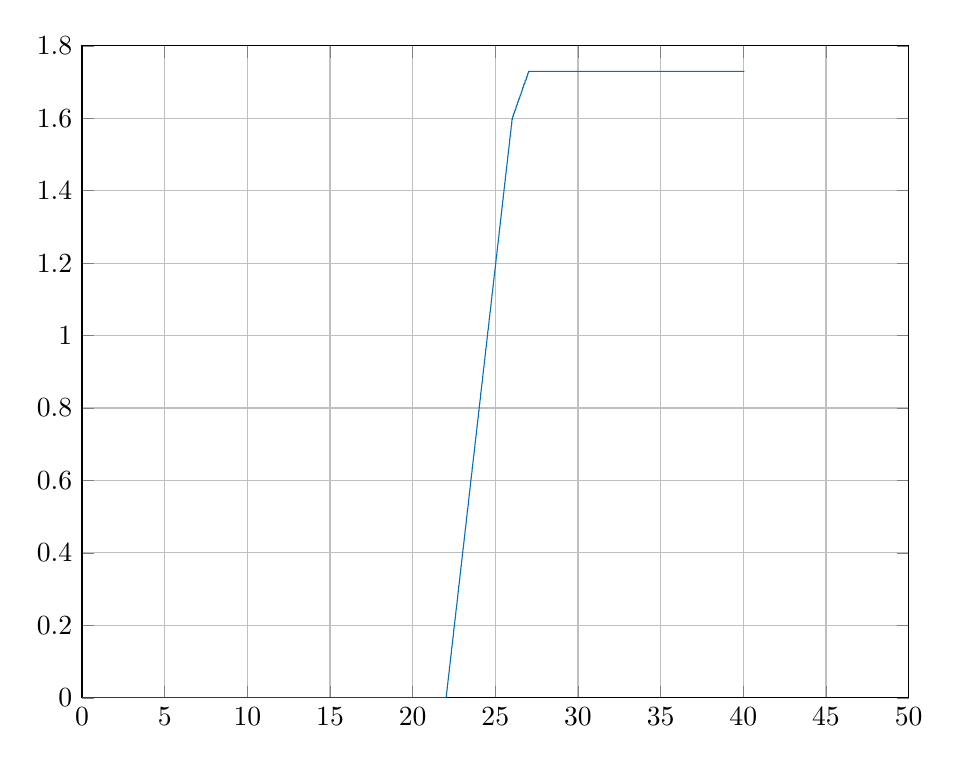
\begin{tikzpicture}

\begin{axis}[%
width=4.133in,
height=3.26in,
at={(0.693in,0.44in)},
scale only axis,
xmin=0,
xmax=50,
xmajorgrids,
ymin=0,
ymax=1.8,
ymajorgrids,
axis background/.style={fill=white}
]
\addplot [color=mycolor1,solid,forget plot]
  table[row sep=crcr]{%
0	0\\
0.0177441540000001	0\\
0.0327040630000001	0\\
0.0478449689999996	0\\
0.0659545939999996	0\\
0.080935841	0\\
0.095923176	0\\
0.11195197	0\\
0.128055795	0\\
0.143941748	0\\
0.159967933999999	0\\
0.176042313999999	0\\
0.191954450999999	0\\
0.208009254	0\\
0.22399488	0\\
0.239953013999999	0\\
0.256054853999999	0\\
0.272063669	0\\
0.288027004	0\\
0.303887813	0\\
0.319971607	0\\
0.335942635	0\\
0.352025743	0\\
0.3679568	0\\
0.383953943	0\\
0.399997912	0\\
0.415998250999999	0\\
0.431831394	0\\
0.447814032000001	0\\
0.463808589999999	0\\
0.479903010999999	0\\
0.495925008	0\\
0.511948347	0\\
0.528016396999999	0\\
0.543863147999999	0\\
0.562388751999999	0\\
0.577608655	0\\
0.592719001999999	0\\
0.608161168000001	0\\
0.624069551	0\\
0.639885296999999	0\\
0.655866359	0\\
0.671987365999999	0\\
0.68802496	0\\
0.703813795999999	0\\
0.719840768	0\\
0.738192618	0\\
0.753498854999999	0\\
0.768784837	0\\
0.784015643	0\\
0.79988878	0\\
0.815969871	0\\
0.831983674	0\\
0.848057242	0\\
0.863854896999999	0\\
0.879894759999999	0\\
0.896003269	0\\
0.911933238999999	0\\
0.928035511999999	0\\
0.943938683999999	0\\
0.960191785999999	0\\
0.975936873000001	0\\
0.991975221	0\\
1.007904933	0\\
1.025398666	0\\
1.040304124	0\\
1.055833496	0\\
1.07185873	0\\
1.090013931	0\\
1.10576894	0\\
1.120861382	0\\
1.13702896	0\\
1.152233154	0\\
1.167848246	0\\
1.183945535	0\\
1.199813575	0\\
1.21810959	0\\
1.233479532	0\\
1.248819967	0\\
1.264119629	0\\
1.2799481	0\\
1.29600457	0\\
1.311980842	0\\
1.327919031	0\\
1.343886916	0\\
1.362367992	0\\
1.377645444	0\\
1.392841231	0\\
1.408078793	0\\
1.424022405	0\\
1.44007512	0\\
1.456127821	0\\
1.472010755	0\\
1.488089533	0\\
1.505276587	0\\
1.52042763	0\\
1.53601755	0\\
1.551942352	0\\
1.567911675	0\\
1.583936325	0\\
1.59989258	0\\
1.615819365	0\\
1.632013797	0\\
1.647959463	0\\
1.663988703	0\\
1.679942628	0\\
1.695987233	0\\
1.712021079	0\\
1.727901406	0\\
1.743933763	0\\
1.762257126	0\\
1.777463037	0\\
1.792770717	0\\
1.808294613	0\\
1.823994137	0\\
1.839996003	0\\
1.856026653	0\\
1.87199263	0\\
1.887955314	0\\
1.903810895	0\\
1.919953914	0\\
1.937593507	0\\
1.952661926	0\\
1.968163942	0\\
1.984178283	0\\
1.999975183	0\\
2.017791296	0\\
2.033056711	0\\
2.047987846	0\\
2.063870266	0\\
2.079834083	0\\
2.096071024	0\\
2.111796419	0\\
2.128044492	0\\
2.143898936	0\\
2.162297373	0\\
2.177444796	0\\
2.192580046	0\\
2.208046917	0\\
2.223993811	0\\
2.239942403	0\\
2.255908685	0\\
2.271844786	0\\
2.290082946	0\\
2.305663551	0\\
2.321427334	0\\
2.337415825	0\\
2.353051482	0\\
2.368230299	0\\
2.384770288	0\\
2.400381588	0\\
2.416019773	0\\
2.432075243	0\\
2.447866992	0\\
2.464034625	0\\
2.479959588	0\\
2.49605535	0\\
2.511924627	0\\
2.528096842	0\\
2.543935965	0\\
2.562280086	0\\
2.577486766	0\\
2.592615542	0\\
2.607909968	0\\
2.624013005	0\\
2.639972317	0\\
2.656019128	0\\
2.671991098	0\\
2.68783833	0\\
2.70381914	0\\
2.719797684	0\\
2.735945271	0\\
2.751977241	0\\
2.767867978	0\\
2.7839776	0\\
2.799980396	0\\
2.816165123	0\\
2.832033263	0\\
2.847985654	0\\
2.864002992	0\\
2.879987682	0\\
2.895901791	0\\
2.912123187	0\\
2.928500747	0\\
2.943946666	0\\
2.959812605	0\\
2.976001123	0\\
2.991910687	0\\
3.0078866	0\\
3.024033743	0\\
3.039833721	0\\
3.055898507	0\\
3.071898381	0\\
3.088173756	0\\
3.104241709	0\\
3.119908618	0\\
3.135877983	0\\
3.151981441	0\\
3.167814753	0\\
3.184016414	0\\
3.200035055	0\\
3.215996707	0\\
3.232054362	0\\
3.247981445	0\\
3.264166714	0\\
3.279790125	0\\
3.296012658	0\\
3.311932396	0\\
3.328156619	0\\
3.343862637	0\\
3.360331353	0\\
3.376034386	0\\
3.391958477	0\\
3.407941351	0\\
3.423828912	0\\
3.442126699	0\\
3.457365924	0\\
3.472518824	0\\
3.487868274	0\\
3.503812755	0\\
3.519945999	0\\
3.536039249	0\\
3.551938139	0\\
3.568311326	0\\
3.58398362	0\\
3.599969341	0\\
3.615951755	0\\
3.63205545	0\\
3.64796565	0\\
3.665660884	0\\
3.680830758	0\\
3.696031371	0\\
3.711993129	0\\
3.728110995	0\\
3.743985369	0\\
3.760051875	0\\
3.775931153	0\\
3.792102727	0\\
3.808065336	0\\
3.823949485	0\\
3.839914836	0\\
3.856126292	0\\
3.873129683	0\\
3.888415745	0\\
3.904082118	0\\
3.919984447	0\\
3.936797435	0\\
3.95218989	0\\
3.968030944	0\\
3.983982969	0\\
4.000019606	0\\
4.01792116	0\\
4.032913303	0\\
4.047921539	0\\
4.063861382	0\\
4.079857392	0\\
4.095891563	0\\
4.111924659	0\\
4.128192669	0\\
4.143978449	0\\
4.160134024	0\\
4.175925001	0\\
4.191796591	0\\
4.208089832	0\\
4.223946351	0\\
4.239814982	0\\
4.255999085	0\\
4.271969471	0\\
4.290295194	0\\
4.305524384	0\\
4.320741453	0\\
4.335983263	0\\
4.351886062	0\\
4.368028138	0\\
4.383969334	0\\
4.399897934	0\\
4.415925558	0\\
4.431869626	0\\
4.447996477	0\\
4.46381962	0\\
4.479957766	0\\
4.495888877	0\\
4.511978467	0\\
4.527944261	0\\
4.544003875	0\\
4.560241184	0\\
4.575958202	0\\
4.592020126	0\\
4.607920568	0\\
4.624013937	0\\
4.640030653	0\\
4.655955594	0\\
4.671990289	0\\
4.688046214	0\\
4.703806353	0\\
4.719801313	0\\
4.736013502	0\\
4.751897951	0\\
4.768033836	0\\
4.784005832	0\\
4.799899736	0\\
4.815913036	0\\
4.83196671	0\\
4.847775381	0\\
4.863984264	0\\
4.879931643	0\\
4.896051845	0\\
4.911995762	0\\
4.92815309	0\\
4.94391307	0\\
4.960371144	0\\
4.975975883	0\\
4.991936031	0\\
5.00796669	0\\
5.025225409	0\\
5.040174419	0\\
5.055830857	0\\
5.071826165	0\\
5.087915419	0\\
5.103793775	0\\
5.119982737	0\\
5.13764764	0\\
5.152925242	0\\
5.168468381	0\\
5.183880225	0\\
5.199997693	0\\
5.215913877	0\\
5.231898023	0\\
5.247995057	0\\
5.2637976	0\\
5.279791141	0\\
5.296316409	0\\
5.311987624	0\\
5.328189245	0\\
5.343948408	0\\
5.359967983	0\\
5.375954299	0\\
5.391856128	0\\
5.408098391	0\\
5.424079379	0\\
5.440023342	0\\
5.456021868	0\\
5.471990165	0\\
5.488435392	0\\
5.503975324	0\\
5.519860487	0\\
5.535996266	0\\
5.552034071	0\\
5.567791657	0\\
5.583803568	0\\
5.600058789	0\\
5.615944598	0\\
5.632002603	0\\
5.647977485	0\\
5.664107499	0\\
5.679982405	0\\
5.695809307	0\\
5.711927927	0\\
5.727864808	0\\
5.743947707	0\\
5.760158351	0\\
5.775988783	0\\
5.792046087	0\\
5.808040178	0\\
5.823975249	0\\
5.839938834	0\\
5.856000936	0\\
5.871980058	0\\
5.888114707	0\\
5.903881931	0\\
5.922154549	0\\
5.935949996	0\\
5.952079521	0\\
5.967914484	0\\
5.983887847	0\\
6.00001967	0\\
6.018431561	0\\
6.033455699	0\\
6.048482665	0\\
6.063855193	0\\
6.07987279	0\\
6.095898001	0\\
6.111976692	0\\
6.128136278	0\\
6.143940917	0\\
6.159904689	0\\
6.175983181	0\\
6.191947174	0\\
6.207838687	0\\
6.224096146	0\\
6.239995549	0\\
6.256025953	0\\
6.271936895	0\\
6.2881028	0\\
6.303821208	0\\
6.319907718	0\\
6.33602018	0\\
6.351954771	0\\
6.367979261	0\\
6.383979535	0\\
6.3999932	0\\
6.415959658	0\\
6.431813065	0\\
6.44795526	0\\
6.46633681	0\\
6.481640492	0\\
6.496800582	0\\
6.512015123	0\\
6.528007565	0\\
6.544001335	0\\
6.560166974	0\\
6.575941672	0\\
6.591818356	0\\
6.607989749	0\\
6.623906393	0\\
6.64011637	0\\
6.655979844	0\\
6.673691636	0\\
6.688914219	0\\
6.704891777	0\\
6.720183131	0\\
6.737123565	0\\
6.752308488	0\\
6.768028357	0\\
6.783980568	0\\
6.799984341	0\\
6.815967206	0\\
6.83203869	0\\
6.847972771	0\\
6.864023079	0\\
6.879902425	0\\
6.895983262	0\\
6.912068584	0\\
6.928217671	0\\
6.943979611	0\\
6.960208831	0\\
6.975958476	0\\
6.992048525	0\\
7.007884522	0\\
7.025348728	0\\
7.040294171	0\\
7.055880966	0\\
7.071901506	0\\
7.08792888	0\\
7.103913066	0\\
7.120068382	0\\
7.137139436	0\\
7.152855242	0\\
7.168165895	0\\
7.183959671	0\\
7.19999932	0\\
7.215985663	0\\
7.231883992	0\\
7.247973186	0\\
7.263937812	0\\
7.280008721	0\\
7.295851106	0\\
7.312005332	0\\
7.328187843	0\\
7.343982595	0\\
7.36024405	0\\
7.375927101	0\\
7.391989892	0\\
7.4079011	0\\
7.42401634	0\\
7.440028795	0\\
7.456084628	0\\
7.471871999	0\\
7.487989159	0\\
7.504021292	0\\
7.519989669	0\\
7.536008014	0\\
7.551949195	0\\
7.567858875	0\\
7.583935748	0\\
7.601006903	0\\
7.616333011	0\\
7.631832045	0\\
7.648012658	0\\
7.66422105	0\\
7.679991222	0\\
7.695870973	0\\
7.711873373	0\\
7.728006439	0\\
7.743939256	0\\
7.76020953	0\\
7.775971928	0\\
7.792052602	0\\
7.807974727	0\\
7.823995777	0\\
7.840030888	0\\
7.855979139	0\\
7.872011384	0\\
7.8880804	0\\
7.903981492	0\\
7.920021161	0\\
7.93706545	0\\
7.952477327	0\\
7.9678801	0\\
7.983891723	0\\
8.000016786	0\\
8.017869878	0\\
8.032826874	0\\
8.047843233	0\\
8.065963524	0\\
8.080942145	0\\
8.096041817	0\\
8.112014951	0\\
8.12803528	0\\
8.14397842	0\\
8.16001178	0\\
8.176267969	0\\
8.191914898	0\\
8.207940751	0\\
8.224000021	0\\
8.240027206	0\\
8.256005689	0\\
8.272060388	0\\
8.288060868	0\\
8.30464051	0\\
8.320066414	0\\
8.335981801	0\\
8.352041405	0\\
8.367962458	0\\
8.383991149	0\\
8.399972366	0\\
8.416015853	0\\
8.432958448	0\\
8.448360829	0\\
8.463990804	0\\
8.480266458	0\\
8.495865174	0\\
8.511956939	0\\
8.527865723	0\\
8.544168528	0\\
8.559968157	0\\
8.578390398	0\\
8.593594679	0\\
8.608849229	0\\
8.624003037	0\\
8.640080341	0\\
8.655987797	0\\
8.671984308	0\\
8.687931107	0\\
8.704159782	0\\
8.719962013	0\\
8.735946497	0\\
8.752022388	0\\
8.767927688	0\\
8.783984821	0\\
8.800003878	0\\
8.816004223	0\\
8.831966095	0\\
8.848040975	0\\
8.863999835	0\\
8.880144963	0\\
8.895806699	0\\
8.912055063	0\\
8.927921969	0\\
8.944068836	0\\
8.959911623	0\\
8.978394041	0\\
8.993690196	0\\
9.008788051	0\\
9.023814294	0\\
9.041908105	0\\
9.05681926	0\\
9.071835365	0\\
9.087841756	0\\
9.103845233	0\\
9.119976837	0\\
9.136027025	0\\
9.151993408	0\\
9.167967223	0\\
9.183994778	0\\
9.199965717	0\\
9.215891879	0\\
9.231996951	0\\
9.247892359	0\\
9.263988631	0\\
9.280002711	0\\
9.295985623	0\\
9.311957464	0\\
9.327999411	0\\
9.344179888	0\\
9.360029036	0\\
9.376214415	0\\
9.392500602	0\\
9.408018805	0\\
9.423992344	0\\
9.439977644	0\\
9.455994021	0\\
9.472021477	0\\
9.488143487	0\\
9.50406149	0\\
9.519982771	0\\
9.53603548	0\\
9.552021988	0\\
9.567994715	0\\
9.584045985	0\\
9.599980426	0\\
9.616004284	0\\
9.631946195	0\\
9.648059476	0\\
9.663985559	0\\
9.679989567	0\\
9.69599361	0\\
9.711961915	0\\
9.727990195	0\\
9.744101561	0\\
9.759973811	0\\
9.778293465	0\\
9.793577786	0\\
9.808858878	0\\
9.824244693	0\\
9.840290734	0\\
9.856116657	0\\
9.872206048	0\\
9.887930688	0\\
9.903899309	0\\
9.919951271	0\\
9.935977203	0\\
9.951984689	0\\
9.967981481	0\\
9.983956633	0\\
9.999947442	0\\
10.017871321	0\\
10.032808961	0\\
10.047859833	0\\
10.063820433	0\\
10.0819286	0\\
10.09690558	0\\
10.112008278	0\\
10.127976725	0\\
10.144209833	0\\
10.159980776	0\\
10.176072019	0\\
10.192019298	0\\
10.207919569	0\\
10.223870053	0\\
10.239996002	0\\
10.25602208	0\\
10.272043914	0\\
10.28804911	0\\
10.304009835	0\\
10.319993903	0\\
10.336057205	0\\
10.352030243	0\\
10.367956325	0\\
10.384016425	0\\
10.399949676	0\\
10.415887273	0\\
10.431963201	0\\
10.448001658	0\\
10.46402966	0\\
10.480015026	0\\
10.495952148	0\\
10.511976326	0\\
10.5279805	0\\
10.544210234	0\\
10.559986281	0\\
10.575948973	0\\
10.591905897	0\\
10.608046685	0\\
10.623974856	0\\
10.639982006	0\\
10.656007648	0\\
10.672016717	0\\
10.688027015	0\\
10.703883115	0\\
10.719850408	0\\
10.736036028	0\\
10.751966715	0\\
10.768060426	0\\
10.784009615	0\\
10.799861772	0\\
10.815977265	0\\
10.832009553	0\\
10.847977785	0\\
10.864036139	0\\
10.88002107	0\\
10.896019403	0\\
10.911838149	0\\
10.927964589	0\\
10.944132473	0\\
10.960012842	0\\
10.97599494	0\\
10.991880004	0\\
11.007970899	0\\
11.025414481	0\\
11.040451894	0\\
11.055869466	0\\
11.071919421	0\\
11.087924862	0\\
11.103969424	0\\
11.1199788	0\\
11.135877788	0\\
11.151980131	0\\
11.167941124	0\\
11.183995078	0\\
11.200015884	0\\
11.215937089	0\\
11.232019305	0\\
11.248020617	0\\
11.26421936	0\\
11.280012	0\\
11.296021746	0\\
11.312080644	0\\
11.328057691	0\\
11.344028408	0\\
11.360011019	0\\
11.376003706	0\\
11.391936738	0\\
11.407981734	0\\
11.424002395	0\\
11.440014917	0\\
11.45609619	0\\
11.472070065	0\\
11.488103465	0\\
11.5039031	0\\
11.520077922	0\\
11.536003773	0\\
11.551989733	0\\
11.567961579	0\\
11.584026304	0\\
11.599964638	0\\
11.615866219	0\\
11.632051283	0\\
11.648008565	0\\
11.663991783	0\\
11.679955904	0\\
11.695908896	0\\
11.712044954	0\\
11.727984646	0\\
11.744266289	0\\
11.760126251	0\\
11.7760434	0\\
11.792132146	0\\
11.808050886	0\\
11.823997807	0\\
11.84004679	0\\
11.855996079	0\\
11.872030726	0\\
11.888012132	0\\
11.90389773	0\\
11.919992051	0\\
11.935992807	0\\
11.95189877	0\\
11.967868711	0\\
11.984037355	0\\
12.000105929	0\\
12.017849286	0\\
12.032768543	0\\
12.047866061	0\\
12.063880419	0\\
12.079877976	0\\
12.098046519	0\\
12.113407982	0\\
12.128578276	0\\
12.14398879	0\\
12.159980736	0\\
12.176133999	0\\
12.191915091	0\\
12.208001663	0\\
12.224002396	0\\
12.239964929	0\\
12.255964619	0\\
12.272018179	0\\
12.287907709	0\\
12.303960852	0\\
12.319980397	0\\
12.335941135	0\\
12.351983059	0\\
12.367987037	0\\
12.384113476	0\\
12.400041719	0\\
12.416061042	0\\
12.431941691	0\\
12.447990776	0\\
12.46400612	0\\
12.47986539	0\\
12.496005331	0\\
12.511977477	0\\
12.527990866	0\\
12.544075412	0\\
12.560051507	0\\
12.576208672	0\\
12.591987399	0\\
12.607988185	0\\
12.623998292	0\\
12.640042872	0\\
12.655954371	0\\
12.671993002	0\\
12.688069214	0\\
12.704052035	0\\
12.720157683	0\\
12.735883019	0\\
12.751988071	0\\
12.767953513	0\\
12.784022603	0\\
12.79994475	0\\
12.815851826	0\\
12.831979317	0\\
12.848006828	0\\
12.864024507	0\\
12.879993846	0\\
12.896013505	0\\
12.912028027	0\\
12.927939231	0\\
12.94406223	0\\
12.959992479	0\\
12.978385834	0\\
12.993673517	0\\
13.008884356	0\\
13.023873171	0\\
13.039965823	0\\
13.055962863	0\\
13.072056005	0\\
13.088051354	0\\
13.103908324	0\\
13.119826742	0\\
13.135977399	0\\
13.151916194	0\\
13.168070177	0\\
13.18398576	0\\
13.199890941	0\\
13.215990689	0\\
13.231990683	0\\
13.248005491	0\\
13.263988195	0\\
13.280023099	0\\
13.295914622	0\\
13.3120289	0\\
13.327973192	0\\
13.3463917	0\\
13.361635521	0\\
13.376936742	0\\
13.392542949	0\\
13.407984984	0\\
13.423990415	0\\
13.440035161	0\\
13.456027312	0\\
13.472029757	0\\
13.488019035	0\\
13.504048668	0\\
13.519997101	0\\
13.535957424	0\\
13.551978436	0\\
13.567960935	0\\
13.583982097	0\\
13.600088893	0\\
13.616051723	0\\
13.632095198	0\\
13.647936911	0\\
13.664018976	0\\
13.679929405	0\\
13.696115557	0\\
13.712088791	0\\
13.728079724	0\\
13.744146188	0\\
13.760004076	0\\
13.776138129	0\\
13.791990433	0\\
13.808319523	0\\
13.823991519	0\\
13.840876282	0\\
13.856198395	0\\
13.872022927	0\\
13.88799893	0\\
13.903902853	0\\
13.920299171	0\\
13.936524143	0\\
13.952003133	0\\
13.967922164	0\\
13.984021356	0\\
14.000004302	0\\
14.021512803	0\\
14.033500279	0\\
14.048825728	0\\
14.064094519	0\\
14.079982062	0\\
14.096036069	0\\
14.111978945	0\\
14.127970598	0\\
14.144272802	0\\
14.159927968	0\\
14.176001765	0\\
14.191993996	0\\
14.208044255	0\\
14.224030353	0\\
14.239899612	0\\
14.25595932	0\\
14.271973075	0\\
14.28807093	0\\
14.303881156	0\\
14.319956078	0\\
14.337491235	0\\
14.352804817	0\\
14.368146496	0\\
14.384045512	0\\
14.399862218	0\\
14.415813551	0\\
14.431962165	0\\
14.447932542	0\\
14.464199591	0\\
14.47987596	0\\
14.496005858	0\\
14.511931121	0\\
14.527984224	0\\
14.543959983	0\\
14.559920262	0\\
14.576162621	0\\
14.591981038	0\\
14.608046856	0\\
14.62399606	0\\
14.640035955	0\\
14.655874969	0\\
14.67200585	0\\
14.687913297	0\\
14.703887227	0\\
14.720035739	0\\
14.736084322	0\\
14.751996589	0\\
14.767982716	0\\
14.784021955	0\\
14.799951995	0\\
14.815974284	0\\
14.832722157	0\\
14.848035872	0\\
14.86398905	0\\
14.880026604	0\\
14.896024939	0\\
14.912215675	0\\
14.927989651	0\\
14.943997957	0\\
14.959906851	0\\
14.978305886	0\\
14.99354199	0\\
15.008697568	0\\
15.023974395	0\\
15.039986789	0\\
15.056140917	0\\
15.072027932	0\\
15.087898911	0\\
15.104072529	0\\
15.119999799	0\\
15.136014341	0\\
15.151948685	0\\
15.16794009	0\\
15.183979463	0\\
15.200022249	0\\
15.215902045	0\\
15.231979085	0\\
15.24810982	0\\
15.26400462	0\\
15.279983627	0\\
15.296015789	0\\
15.311988997	0\\
15.327958147	0\\
15.344116503	0\\
15.359944198	0\\
15.375985619	0\\
15.391964544	0\\
15.407926139	0\\
15.423929022	0\\
15.440027877	0\\
15.4559316	0\\
15.471922784	0\\
15.487959992	0\\
15.503849215	0\\
15.522218674	0\\
15.537355028	0\\
15.552485878	0\\
15.567856399	0\\
15.583983553	0\\
15.599907845	0\\
15.615964183	0\\
15.631958534	0\\
15.64799247	0\\
15.663977415	0\\
15.679929334	0\\
15.695828736	0\\
15.712003932	0\\
15.72812514	0\\
15.744129129	0\\
15.759839239	0\\
15.776051962	0\\
15.791962243	0\\
15.807942971	0\\
15.824014363	0\\
15.840027182	0\\
15.855982539	0\\
15.872008117	0\\
15.887972795	0\\
15.903826785	0\\
15.919920663	0\\
15.935967355	0\\
15.95200946	0\\
15.967943705	0\\
15.983972538	0\\
15.999983157	0\\
16.018615015	0\\
16.031993003	0\\
16.048060554	0\\
16.064007484	0\\
16.079901392	0\\
16.095854435	0\\
16.111999047	0\\
16.128037352	0\\
16.144240554	0\\
16.159954101	0\\
16.175951184	0\\
16.191984654	0\\
16.207904056	0\\
16.223985031	0\\
16.240024681	0\\
16.25600208	0\\
16.272006995	0\\
16.288044368	0\\
16.304065686	0\\
16.319995551	0\\
16.335958025	0\\
16.352009455	0\\
16.367880078	0\\
16.38399931	0\\
16.399958407	0\\
16.415849514	0\\
16.431883881	0\\
16.447992115	0\\
16.464002217	0\\
16.480128507	0\\
16.495935629	0\\
16.511965451	0\\
16.527942849	0\\
16.544002784	0\\
16.559951852	0\\
16.576310388	0\\
16.591993916	0\\
16.607981093	0\\
16.624099508	0\\
16.639977816	0\\
16.655957981	0\\
16.672075781	0\\
16.687981617	0\\
16.70408034	0\\
16.720016419	0\\
16.7359338	0\\
16.752928353	0\\
16.768076001	0\\
16.784042128	0\\
16.799941782	0\\
16.816403911	0\\
16.831945972	0\\
16.848033424	0\\
16.86404063	0\\
16.880056043	0\\
16.89597555	0\\
16.911809413	0\\
16.927964491	0\\
16.943859189	0\\
16.959847547	0\\
16.976306144	0\\
16.991895648	0\\
17.007861192	0\\
17.023903461	0\\
17.039888521	0\\
17.055981314	0\\
17.071804681	0\\
17.08812132	0\\
17.103986067	0\\
17.11994946	0\\
17.135943308	0\\
17.152028495	0\\
17.167997112	0\\
17.183813738	0\\
17.1999706	0\\
17.216001494	0\\
17.231945523	0\\
17.248143254	0\\
17.263959356	0\\
17.279957697	0\\
17.295903573	0\\
17.311831899	0\\
17.327913376	0\\
17.34387256	0\\
17.360021005	0\\
17.376265783	0\\
17.392021055	0\\
17.407958846	0\\
17.424052004	0\\
17.440041537	0\\
17.455980248	0\\
17.47205077	0\\
17.487902924	0\\
17.503972557	0\\
17.519909292	0\\
17.535974259	0\\
17.551906023	0\\
17.567973181	0\\
17.583989841	0\\
17.599989014	0\\
17.615818706	0\\
17.631799887	0\\
17.64796211	0\\
17.66402742	0\\
17.680030102	0\\
17.695854282	0\\
17.711905321	0\\
17.727900065	0\\
17.744114573	0\\
17.75999217	0\\
17.776111038	0\\
17.791797316	0\\
17.808062441	0\\
17.823913438	0\\
17.840021682	0\\
17.855995502	0\\
17.872057927	0\\
17.88793406	0\\
17.90402632	0\\
17.919969605	0\\
17.936015152	0\\
17.952047514	0\\
17.967998953	0\\
17.98408643	0\\
17.999937903	0\\
18.017713904	0\\
18.032926989	0\\
18.048076682	0\\
18.063924107	0\\
18.080003085	0\\
18.096008291	0\\
18.111842246	0\\
18.130062683	0\\
18.145491549	0\\
18.160759238	0\\
18.175956101	0\\
18.191884821	0\\
18.20806147	0\\
18.224692697	0\\
18.239952728	0\\
18.256008258	0\\
18.272024733	0\\
18.288010349	0\\
18.30410588	0\\
18.320001355	0\\
18.335972967	0\\
18.351979796	0\\
18.36816057	0\\
18.383868069	0\\
18.400025477	0\\
18.416136989	0\\
18.431947889	0\\
18.447949276	0\\
18.463946043	0\\
18.479997801	0\\
18.496050152	0\\
18.511806667	0\\
18.527798792	0\\
18.543893029	0\\
18.559880903	0\\
18.576054051	0\\
18.591822555	0\\
18.607864675	0\\
18.623982842	0\\
18.640034433	0\\
18.655940578	0\\
18.671970701	0\\
18.688088237	0\\
18.704055742	0\\
18.719847187	0\\
18.735947129	0\\
18.751992392	0\\
18.767902927	0\\
18.783831042	0\\
18.7999934	0\\
18.815810661	0\\
18.834114914	0\\
18.84946709	0\\
18.864867929	0\\
18.880255113	0\\
18.895962589	0\\
18.911859012	0\\
18.927977997	0\\
18.943940977	0\\
18.959923903	0\\
18.976041518	0\\
18.991981506	0\\
19.007935539	0\\
19.025572889	0\\
19.040871928	0\\
19.056438628	0\\
19.072266862	0\\
19.087987123	0\\
19.104017448	0\\
19.120041113	0\\
19.136089582	0\\
19.152001241	0\\
19.167970653	0\\
19.183993411	0\\
19.19997326	0\\
19.217370569	0\\
19.232709265	0\\
19.248086704	0\\
19.263974539	0\\
19.280053441	0\\
19.295960011	0\\
19.311846466	0\\
19.330104587	0\\
19.345462389	0\\
19.36091123	0\\
19.376104842	0\\
19.391941061	0\\
19.407895005	0\\
19.424153682	0\\
19.439978196	0\\
19.455975314	0\\
19.472029896	0\\
19.487922857	0\\
19.50403235	0\\
19.519984596	0\\
19.536018948	0\\
19.552021052	0\\
19.567933364	0\\
19.584057507	0\\
19.599982401	0\\
19.616378024	0\\
19.631959547	0\\
19.647867944	0\\
19.663884525	0\\
19.680028676	0\\
19.69598001	0\\
19.711797359	0\\
19.729901931	0\\
19.745080392	0\\
19.760194592	0\\
19.77598209	0\\
19.791910871	0\\
19.808114813	0\\
19.823910719	0\\
19.839977941	0\\
19.856102042	0\\
19.872069051	0\\
19.887886331	0\\
19.904063416	0\\
19.919879187	0\\
19.935990063	0\\
19.952153276	0\\
19.967911568	0\\
19.984041665	0\\
19.999969177	0\\
20.017754685	0\\
20.033065576	0\\
20.048261028	0\\
20.065148395	0\\
20.080584776	0\\
20.095921297	0\\
20.112314658	0\\
20.128072212	0\\
20.144050322	0\\
20.160008674	0\\
20.176244886	0\\
20.191946088	0\\
20.208192053	0\\
20.223937571	0\\
20.240101997	0\\
20.255949027	0\\
20.272073862	0\\
20.288048639	0\\
20.303961711	0\\
20.320062529	0\\
20.336051327	0\\
20.351867158	0\\
20.367998558	0\\
20.384235131	0\\
20.399970861	0\\
20.416047321	0\\
20.432002035	0\\
20.447985038	0\\
20.463823328	0\\
20.479886681	0\\
20.495986982	0\\
20.511926494	0\\
20.527922729	0\\
20.543957572	0\\
20.559990106	0\\
20.575967763	0\\
20.592058742	0\\
20.60784029	0\\
20.623964623	0\\
20.639915171	0\\
20.655942033	0\\
20.672022121	0\\
20.687986574	0\\
20.707530295	0\\
20.7198142	0\\
20.735799943	0\\
20.754076883	0\\
20.769131774	0\\
20.785242884	0\\
20.800413404	0\\
20.815900959	0\\
20.831911751	0\\
20.847991349	0\\
20.864215246	0\\
20.880172489	0\\
20.89604119	0\\
20.912091578	0\\
20.927945847	0\\
20.944081173	0\\
20.960066684	0\\
20.975969002	0\\
20.991931671	0\\
21.007976778	0\\
21.025607157	0\\
21.041084259	0\\
21.056381035	0\\
21.071975516	0\\
21.08800851	0\\
21.104036106	0\\
21.11978888	0\\
21.136058816	0\\
21.151994684	0\\
21.167953509	0\\
21.184001052	0\\
21.199977548	0\\
21.215797052	0\\
21.234055508	0\\
21.249365023	0\\
21.264517231	0\\
21.280016451	0\\
21.295960836	0\\
21.311862378	0\\
21.327983413	0\\
21.34406115	0\\
21.359918185	0\\
21.375870588	0\\
21.391958276	0\\
21.408024456	0\\
21.423858845	0\\
21.439904702	0\\
21.455890771	0\\
21.472065636	0\\
21.487990324	0\\
21.503924697	0\\
21.519952902	0\\
21.536053434	0\\
21.552156546	0\\
21.567988841	0\\
21.583994477	0\\
21.59996743	0\\
21.615992246	0\\
21.655064028	0\\
21.670173849	0\\
21.686191848	0\\
21.702176256	0\\
21.718242571	0\\
21.734196731	0\\
21.752411665	0\\
21.767800269	0\\
21.783079991	0\\
21.798362695	0\\
21.814357483	0\\
21.830303609	0\\
21.846278672	0\\
21.862192804	0\\
21.880667552	0\\
21.895776652	0\\
21.910926669	0\\
21.926283994	0\\
21.944665708	0\\
21.959741178	0\\
21.974922207	0\\
21.990247147	0\\
22.006397717	0\\
22.023988324	0.00196265250093623\\
22.039055139	0.00588782309712144\\
22.05430491	0.0137378271094637\\
22.070331314	0.0180483095532901\\
22.086381205	0.0243211223106177\\
22.102324425	0.0349037381639916\\
22.11844384	0.0372525409112749\\
22.134320397	0.0451024846421164\\
22.150300566	0.0509900495807489\\
22.166279265	0.0568771427074427\\
22.182322897	0.0647266827313098\\
22.198249003	0.0690376659754403\\
22.214245136	0.0753108401078128\\
22.230301005	0.0862812586487168\\
22.246394786	0.0882437976568816\\
22.262230523	0.0960930788631625\\
22.278448973	0.101980106548511\\
22.294239367	0.107866668964832\\
22.310426027	0.115715468385378\\
22.326201298	0.12002687706296\\
22.342466703	0.126300396507757\\
22.358312833	0.136884975424979\\
22.374320144	0.139235086555282\\
22.390375329	0.1470836920051\\
22.406225986	0.15297027106607\\
22.422235792	0.15885635045153\\
22.438465649	0.166704549779748\\
22.454329415	0.171016583078527\\
22.470383371	0.17729046311912\\
22.486352676	0.187875869136671\\
22.502240175	0.192188863893721\\
22.518396709	0.198074482817265\\
22.534244035	0.20396050407154\\
22.550249363	0.209846057649824\\
22.566291798	0.217693447243858\\
22.582415262	0.222005959012147\\
22.5984103	0.228280326950425\\
22.614325262	0.238479535972078\\
22.630270806	0.243180244429294\\
22.64632788	0.249065228270173\\
22.662287485	0.254950792897375\\
22.680877012	0.260835853280376\\
22.696397841	0.268682699723232\\
22.711552355	0.274567647842122\\
22.726574298	0.281232042751927\\
22.742327242	0.28907848018076\\
22.758279839	0.294171497626362\\
22.774478613	0.300056089859967\\
22.790305551	0.309864098850856\\
22.806395373	0.311825621819897\\
22.822354675	0.319671643134187\\
22.838466497	0.325556305588455\\
22.854355785	0.332221740704128\\
22.870407877	0.340067554629623\\
22.88631445	0.345162899144574\\
22.902387617	0.351046943950282\\
22.918459556	0.360853983964899\\
22.934269089	0.36281543667645\\
22.950361492	0.370660705553917\\
22.96629014	0.376936013254002\\
22.982346792	0.383211592093098\\
22.998236221	0.391449238896718\\
23.019628587	0.398115348909671\\
23.031469793	0.403998964688387\\
23.046564953	0.411843965087871\\
23.062298764	0.413805058741265\\
23.078402653	0.421649763121828\\
23.094178311	0.427925287928286\\
23.110200395	0.434201207878475\\
23.127454235	0.44243923506565\\
23.143406326	0.447145421266491\\
23.158732463	0.453028415736072\\
23.174360877	0.462833719844635\\
23.190324647	0.466756188006447\\
23.206298972	0.472638696574248\\
23.222169591	0.478914523300112\\
23.238559523	0.485190794301947\\
23.254371491	0.493428744342509\\
23.270249796	0.500097345551876\\
23.286372482	0.504019054265204\\
23.302282086	0.513823554756014\\
23.318186828	0.517745488092429\\
23.334156421	0.523627574221056\\
23.350343948	0.529903769743589\\
23.366284072	0.536180453424628\\
23.382328887	0.544418667427697\\
23.398255897	0.54912757780595\\
23.414166942	0.556970254100018\\
23.430330648	0.564813053342594\\
23.446383868	0.568734821114503\\
23.462191018	0.574616259106889\\
23.478430311	0.582853268079862\\
23.494241708	0.58716965955018\\
23.510470816	0.595803560963653\\
23.526358042	0.602078852989293\\
23.542700745	0.607960466546468\\
23.558199073	0.615802495024335\\
23.574375386	0.619723769078695\\
23.590330593	0.625604757919442\\
23.606500598	0.635802425644029\\
23.622688537	0.638158989803058\\
23.638185474	0.646793625294386\\
23.654196095	0.653069332399784\\
23.670408415	0.658950332584922\\
23.686326759	0.666791751472149\\
23.702264482	0.670712809654558\\
23.718290795	0.676592967091962\\
23.734374509	0.686790642733639\\
23.750286653	0.689147835126509\\
23.766291469	0.698178695539595\\
23.78234744	0.704059634548842\\
23.798177011	0.709940187011015\\
23.814320352	0.717780776992039\\
23.830228216	0.721701303004489\\
23.846288473	0.727581227441712\\
23.862190859	0.737778817999552\\
23.878302401	0.740136497297147\\
23.894256324	0.749169330642184\\
23.910209326	0.755049696763626\\
23.928327762	0.760929580551688\\
23.943538498	0.768769527628751\\
23.958722043	0.772689834404467\\
23.974378754	0.778568941406616\\
23.990177182	0.789165099570481\\
24.00855221	0.793085353935178\\
24.022871924	0.800159599431706\\
24.038509697	0.807999237029899\\
24.054292439	0.811918937918927\\
24.070268278	0.819758071006196\\
24.086144764	0.823677833565138\\
24.102335473	0.829556682908028\\
24.118289543	0.840153596068286\\
24.134209088	0.844473718510547\\
24.150364932	0.851149686339819\\
24.16630243	0.857028937192202\\
24.18243555	0.862907679862328\\
24.198321486	0.870746222510152\\
24.214354372	0.874665543888288\\
24.230180066	0.880543577384739\\
24.246290664	0.891141544959315\\
24.262274475	0.895862696960028\\
24.278342243	0.90213931593016\\
24.294426776	0.909977518864959\\
24.310343148	0.913896486284602\\
24.326225234	0.92173393147615\\
24.342217303	0.927612348435594\\
24.360546942	0.933890838043761\\
24.375647749	0.942129380591523\\
24.390990519	0.946851919225665\\
24.406294182	0.953128747489676\\
24.422268531	0.962925377587285\\
24.438308004	0.964884472093195\\
24.454332951	0.972721576855379\\
24.470233269	0.978599193509023\\
24.486268323	0.984877768455997\\
24.502342485	0.993116603215289\\
24.518159415	0.997840386602373\\
24.534170077	1.0041175632084\\
24.550332823	1.01391337846501\\
24.56636199	1.01587223259384\\
24.582348102	1.02370850342089\\
24.598328392	1.02958559974022\\
24.61425054	1.03626776577397\\
24.630282536	1.04450715596784\\
24.646314333	1.04922962941131\\
24.66241766	1.05510628110657\\
24.678344394	1.06490084757692\\
24.69437882	1.06685970298689\\
24.710248503	1.07469535768219\\
24.726220501	1.08057182192994\\
24.742386991	1.08725481491809\\
24.758171706	1.09549459045194\\
24.774276598	1.10021825400664\\
24.790359155	1.10609416527933\\
24.806220989	1.11588817418989\\
24.822354658	1.11784657191708\\
24.838330041	1.12568112591984\\
24.854223247	1.13196118509653\\
24.870422163	1.13824142277462\\
24.886866671	1.14688620550705\\
24.902317714	1.15316488005878\\
24.918228638	1.15708174450331\\
24.934330968	1.16687469330637\\
24.950296628	1.16883298478745\\
24.966439927	1.17666733201016\\
24.982181905	1.18294717200749\\
24.998338685	1.18922786462291\\
25.019140482	1.19787345918613\\
25.031151038	1.2021939950681\\
25.04632837	1.21002739740136\\
25.062254328	1.21786106991685\\
25.07828592	1.21981899732522\\
25.094461408	1.22765201807498\\
25.110176998	1.23629723343006\\
25.126163718	1.24062037915038\\
25.142242643	1.24886010114132\\
25.158240413	1.25318127687609\\
25.174292944	1.2590554019773\\
25.19017162	1.26884624490905\\
25.206191876	1.27080433595704\\
25.222269787	1.27863653569562\\
25.238238855	1.28728251649439\\
25.256529852	1.2920137289348\\
25.272086529	1.30025146250009\\
25.28706972	1.30416772230268\\
25.302328479	1.31199963946133\\
25.318327917	1.31983183266723\\
25.334252533	1.32374735391161\\
25.350385947	1.33002802844821\\
25.366357627	1.33826789687623\\
25.382352689	1.34300004128353\\
25.398467113	1.35123770067406\\
25.414221319	1.35515389731171\\
25.430408024	1.36298476920618\\
25.446212433	1.37081574918354\\
25.464439046	1.37473165363319\\
25.479621267	1.38142102021264\\
25.49472912	1.3916193074079\\
25.510384383	1.39398574941582\\
25.526536748	1.40222342759882\\
25.542392689	1.4080963948855\\
25.558391582	1.41396929142831\\
25.574182136	1.42179943970832\\
25.590396774	1.42571482611862\\
25.606315667	1.4324053539943\\
25.622186452	1.44301377537657\\
25.638168271	1.4453784049338\\
25.654182391	1.45320864718292\\
25.670203463	1.45908143988643\\
25.686304702	1.46495295770858\\
25.702142729	1.47278276169963\\
25.720392975	1.47751791749954\\
25.735504011	1.48338923249167\\
25.750497624	1.49399820212478\\
25.766330907	1.49636387362498\\
25.782142986	1.50419302864838\\
25.800180284	1.51202207510228\\
25.815242579	1.51593651993322\\
25.830473416	1.52376508317069\\
25.846232104	1.52850129776014\\
25.862354178	1.53478446038422\\
25.878265906	1.54498187507751\\
25.894347376	1.54734818560242\\
25.91036042	1.55517664296686\\
25.926333271	1.56104822011759\\
25.942327844	1.56691876082406\\
25.958210236	1.57515843310784\\
25.976436178	1.57948482942868\\
25.991580363	1.58617998191716\\
26.006959245	1.59637534990291\\
26.024235248	1.59637511431624\\
26.039267488	1.60224534794807\\
26.054277042	1.60420204283627\\
26.070167825	1.60615867185836\\
26.086260823	1.6061578488929\\
26.102151778	1.612027967353\\
26.118181712	1.61202756894149\\
26.13432692	1.61398360022728\\
26.150200076	1.61593944803289\\
26.1663409	1.61593903980029\\
26.182296298	1.6218086539615\\
26.198312342	1.62180753586554\\
26.214310844	1.62376391987536\\
26.230265631	1.62571947899068\\
26.2462289	1.62696085426466\\
26.262379877	1.63324449311547\\
26.278300511	1.63324449311547\\
26.294359329	1.63520034337774\\
26.310370588	1.63715660875594\\
26.326516458	1.63756843553285\\
26.342636789	1.64343735260555\\
26.358333657	1.64343695052131\\
26.374295671	1.64539328586717\\
26.39031626	1.6473489620994\\
26.406390167	1.64930503146661\\
26.422336635	1.65321736283439\\
26.438388681	1.65321643383888\\
26.454356703	1.65517197721347\\
26.470336431	1.65712793082226\\
26.486230453	1.65908371102238\\
26.502330661	1.66299509418414\\
26.518147054	1.66299459778688\\
26.53417113	1.66494985115996\\
26.550368614	1.6669055064385\\
26.566345426	1.67081714686794\\
26.582350471	1.67277271935071\\
26.598330385	1.67277143950487\\
26.623998244	1.67793273278838\\
26.630175521	1.67834865005335\\
26.646173326	1.6822601578852\\
26.662223168	1.68421582294451\\
26.678223535	1.68421515141987\\
26.694342251	1.68658531711789\\
26.71034016	1.68854049724439\\
26.726521206	1.69440846027549\\
26.74244475	1.69440751093652\\
26.758373091	1.69440652030594\\
26.774301207	1.69636217445991\\
26.79029648	1.69831706327394\\
26.806365657	1.70418391821695\\
26.822282652	1.70418341229416\\
26.838361476	1.70418227585839\\
26.854343001	1.70613702947508\\
26.870395761	1.70809229888722\\
26.886328543	1.71395864369089\\
26.902260285	1.71395798168635\\
26.918198218	1.71395729879783\\
26.934154711	1.71786827082108\\
26.950352974	1.71786612832197\\
26.966294747	1.7237327178115\\
26.982275437	1.72498872266842\\
26.998444123	1.72540639536885\\
27.019333815	1.72931723879723\\
27.031206463	1.72931654577744\\
27.046472644	1.72931612055085\\
27.062339693	1.72931612055085\\
27.078343179	1.72931612055085\\
27.094539878	1.72931612055085\\
27.110444733	1.72931612055085\\
27.126414222	1.72931612055085\\
27.142344233	1.72931612055085\\
27.158330115	1.72931612055085\\
27.174293356	1.72931612055085\\
27.190432098	1.72931612055085\\
27.206248855	1.72931612055085\\
27.222432874	1.72931612055085\\
27.238301631	1.72931612055085\\
27.254303991	1.72931612055085\\
27.270635766	1.72931612055085\\
27.286277598	1.72931612055085\\
27.302338254	1.72931612055085\\
27.318165342	1.72931612055085\\
27.334359687	1.72931612055085\\
27.35033754	1.72931612055085\\
27.366170499	1.72931612055085\\
27.382330342	1.72931612055085\\
27.398309848	1.72931612055085\\
27.414380358	1.72931612055085\\
27.430488232	1.72931612055085\\
27.44643189	1.72931612055085\\
27.462370393	1.72931612055085\\
27.478288669	1.72931612055085\\
27.496720725	1.72931612055085\\
27.511956949	1.72931612055085\\
27.527137468	1.72931612055085\\
27.54240456	1.72931612055085\\
27.558355809	1.72931612055085\\
27.574328803	1.72931612055085\\
27.590349212	1.72931612055085\\
27.606358677	1.72931612055085\\
27.622280033	1.72931612055085\\
27.638364331	1.72931612055085\\
27.654446103	1.72931612055085\\
27.670268076	1.72931612055085\\
27.686173776	1.72931612055085\\
27.719030526	1.72931612055085\\
27.735075717	1.72931612055085\\
27.751093501	1.72931612055085\\
27.767049159	1.72931612055085\\
27.783097455	1.72931612055085\\
27.799098514	1.72931612055085\\
27.815250921	1.72931612055085\\
27.831271767	1.72931612055085\\
27.847312228	1.72931612055085\\
27.863131055	1.72931612055085\\
27.879213798	1.72931612055085\\
27.895208294	1.72931612055085\\
27.911220526	1.72931612055085\\
27.927194339	1.72931612055085\\
27.9431723	1.72931612055085\\
27.959520713	1.72931612055085\\
27.975158815	1.72931612055085\\
27.991204791	1.72931612055085\\
28.007168107	1.72931612055085\\
28.024759165	1.72931612055085\\
28.03916397	1.72931612055085\\
28.055328858	1.72931612055085\\
28.071123681	1.72931612055085\\
28.087179867	1.72931612055085\\
28.103215152	1.72931612055085\\
28.119020403	1.72931612055085\\
28.137149918	1.72931612055085\\
28.152357627	1.72931612055085\\
28.167548669	1.72931612055085\\
28.183226684	1.72931612055085\\
28.199257532	1.72931612055085\\
28.215214795	1.72931612055085\\
28.231215865	1.72931612055085\\
28.247136926	1.72931612055085\\
28.263180299	1.72931612055085\\
28.279120863	1.72931612055085\\
28.295228677	1.72931612055085\\
28.311224629	1.72931612055085\\
28.327183392	1.72931612055085\\
28.343277864	1.72931612055085\\
28.359190185	1.72931612055085\\
28.3752436	1.72931612055085\\
28.391272344	1.72931612055085\\
28.40713285	1.72931612055085\\
28.423215148	1.72931612055085\\
28.439229806	1.72931612055085\\
28.455096114	1.72931612055085\\
28.471240582	1.72931612055085\\
28.487312208	1.72931612055085\\
28.503094577	1.72931612055085\\
28.519025287	1.72931612055085\\
28.53504709	1.72931612055085\\
28.55119733	1.72931612055085\\
28.567215089	1.72931612055085\\
28.583237694	1.72931612055085\\
28.599130151	1.72931612055085\\
28.615188817	1.72931612055085\\
28.631219034	1.72931612055085\\
28.647134746	1.72931612055085\\
28.663187656	1.72931612055085\\
28.679140584	1.72931612055085\\
28.695153261	1.72931612055085\\
28.711199465	1.72931612055085\\
28.727282942	1.72931612055085\\
28.743135156	1.72931612055085\\
28.759504863	1.72931612055085\\
28.775167797	1.72931612055085\\
28.791215195	1.72931612055085\\
28.807197627	1.72931612055085\\
28.823235199	1.72931612055085\\
28.839171798	1.72931612055085\\
28.855274927	1.72931612055085\\
28.871322067	1.72931612055085\\
28.887087775	1.72931612055085\\
28.903315521	1.72931612055085\\
28.919172491	1.72931612055085\\
28.935137292	1.72931612055085\\
28.95115737	1.72931612055085\\
28.967286687	1.72931612055085\\
28.983093588	1.72931612055085\\
28.99921377	1.72931612055085\\
29.020118709	1.72931612055085\\
29.032143043	1.72931612055085\\
29.04743031	1.72931612055085\\
29.063237173	1.72931612055085\\
29.079186787	1.72931612055085\\
29.09521026	1.72931612055085\\
29.111259421	1.72931612055085\\
29.127156918	1.72931612055085\\
29.143218523	1.72931612055085\\
29.15930211	1.72931612055085\\
29.175217517	1.72931612055085\\
29.19122775	1.72931612055085\\
29.207224717	1.72931612055085\\
29.223212618	1.72931612055085\\
29.239281804	1.72931612055085\\
29.255377284	1.72931612055085\\
29.271270126	1.72931612055085\\
29.287193641	1.72931612055085\\
29.303207456	1.72931612055085\\
29.319215696	1.72931612055085\\
29.33522306	1.72931612055085\\
29.351245555	1.72931612055085\\
29.367110493	1.72931612055085\\
29.383232739	1.72931612055085\\
29.399274843	1.72931612055085\\
29.415114943	1.72931612055085\\
29.431206031	1.72931612055085\\
29.447206987	1.72931612055085\\
29.463189241	1.72931612055085\\
29.479206619	1.72931612055085\\
29.495190478	1.72931612055085\\
29.51119154	1.72931612055085\\
29.52958329	1.72931612055085\\
29.544659521	1.72931612055085\\
29.559801903	1.72931612055085\\
29.575254682	1.72931612055085\\
29.591209629	1.72931612055085\\
29.607026912	1.72931612055085\\
29.625414226	1.72931612055085\\
29.640730807	1.72931612055085\\
29.655994353	1.72931612055085\\
29.671139312	1.72931612055085\\
29.687224587	1.72931612055085\\
29.703031675	1.72931612055085\\
29.719074687	1.72931612055085\\
29.735237349	1.72931612055085\\
29.75123185	1.72931612055085\\
29.76724116	1.72931612055085\\
29.783195079	1.72931612055085\\
29.799303985	1.72931612055085\\
29.815245557	1.72931612055085\\
29.831318362	1.72931612055085\\
29.847186559	1.72931612055085\\
29.86317547	1.72931612055085\\
29.879152447	1.72931612055085\\
29.895281118	1.72931612055085\\
29.911228848	1.72931612055085\\
29.927216077	1.72931612055085\\
29.943234113	1.72931612055085\\
29.959540115	1.72931612055085\\
29.977023485	1.72931612055085\\
29.992197578	1.72931612055085\\
30.007443899	1.72931612055085\\
30.02484184	1.72931612055085\\
30.04003791	1.72931612055085\\
30.055263753	1.72931612055085\\
30.071304876	1.72931612055085\\
30.087284849	1.72931612055085\\
30.103217907	1.72931612055085\\
30.119249873	1.72931612055085\\
30.135153627	1.72931612055085\\
30.151063444	1.72931612055085\\
30.167217592	1.72931612055085\\
30.183298259	1.72931612055085\\
30.199232869	1.72931612055085\\
30.215176395	1.72931612055085\\
30.231212958	1.72931612055085\\
30.247380221	1.72931612055085\\
30.263170617	1.72931612055085\\
30.279236067	1.72931612055085\\
30.29524439	1.72931612055085\\
30.311189433	1.72931612055085\\
30.329670975	1.72931612055085\\
30.344985235	1.72931612055085\\
30.360344327	1.72931612055085\\
30.375516236	1.72931612055085\\
30.391363579	1.72931612055085\\
30.407215568	1.72931612055085\\
30.423240823	1.72931612055085\\
30.439305985	1.72931612055085\\
30.455232388	1.72931612055085\\
30.471254166	1.72931612055085\\
30.487148531	1.72931612055085\\
30.505375119	1.72931612055085\\
30.520681111	1.72931612055085\\
30.536056068	1.72931612055085\\
30.551319635	1.72931612055085\\
30.567217745	1.72931612055085\\
30.583058304	1.72931612055085\\
30.599221912	1.72931612055085\\
30.615259079	1.72931612055085\\
30.631271805	1.72931612055085\\
30.647229989	1.72931612055085\\
30.663458166	1.72931612055085\\
30.679151412	1.72931612055085\\
30.695233676	1.72931612055085\\
30.711058887	1.72931612055085\\
30.727045985	1.72931612055085\\
30.75490632	1.72931612055085\\
30.763624625	1.72931612055085\\
30.775545112	1.72931612055085\\
30.791088079	1.72931612055085\\
30.807297415	1.72931612055085\\
30.825937383	1.72931612055085\\
30.839252786	1.72931612055085\\
30.855233205	1.72931612055085\\
30.871216978	1.72931612055085\\
30.887219999	1.72931612055085\\
30.903235975	1.72931612055085\\
30.919210786	1.72931612055085\\
30.935233757	1.72931612055085\\
30.951213231	1.72931612055085\\
30.967235358	1.72931612055085\\
30.983188431	1.72931612055085\\
30.999216774	1.72931612055085\\
31.017936925	1.72931612055085\\
31.033276264	1.72931612055085\\
31.04868307	1.72931612055085\\
31.064165665	1.72931612055085\\
31.079514664	1.72931612055085\\
31.095351714	1.72931612055085\\
31.111034839	1.72931612055085\\
31.127148068	1.72931612055085\\
31.143199096	1.72931612055085\\
31.159345436	1.72931612055085\\
31.175212348	1.72931612055085\\
31.191184266	1.72931612055085\\
31.207252758	1.72931612055085\\
31.223225039	1.72931612055085\\
31.239134144	1.72931612055085\\
31.255560974	1.72931612055085\\
31.27107972	1.72931612055085\\
31.287171758	1.72931612055085\\
31.303247139	1.72931612055085\\
31.319209483	1.72931612055085\\
31.335190363	1.72931612055085\\
31.351095654	1.72931612055085\\
31.367107767	1.72931612055085\\
31.38320764	1.72931612055085\\
31.399308458	1.72931612055085\\
31.415100041	1.72931612055085\\
31.431041635	1.72931612055085\\
31.447188292	1.72931612055085\\
31.463090824	1.72931612055085\\
31.479182738	1.72931612055085\\
31.495294445	1.72931612055085\\
31.51151139	1.72931612055085\\
31.527134786	1.72931612055085\\
31.54319205	1.72931612055085\\
31.559301783	1.72931612055085\\
31.57521718	1.72931612055085\\
31.591226806	1.72931612055085\\
31.607193407	1.72931612055085\\
31.623235537	1.72931612055085\\
31.639127693	1.72931612055085\\
31.655226272	1.72931612055085\\
31.671139659	1.72931612055085\\
31.687317576	1.72931612055085\\
31.703727255	1.72931612055085\\
31.71931342	1.72931612055085\\
31.735231352	1.72931612055085\\
31.751460681	1.72931612055085\\
31.767177218	1.72931612055085\\
31.783250798	1.72931612055085\\
31.799188046	1.72931612055085\\
31.815097946	1.72931612055085\\
31.831226044	1.72931612055085\\
31.847192508	1.72931612055085\\
31.863226095	1.72931612055085\\
31.879218741	1.72931612055085\\
31.89519377	1.72931612055085\\
31.911405468	1.72931612055085\\
31.927253908	1.72931612055085\\
31.94306244	1.72931612055085\\
31.961186856	1.72931612055085\\
31.976265233	1.72931612055085\\
31.991262475	1.72931612055085\\
32.007106942	1.72931612055085\\
32.023086773	1.72931612055085\\
32.040123036	1.72931612055085\\
32.055169901	1.72931612055085\\
32.072137629	1.72931612055085\\
32.0874407	1.72931612055085\\
32.103262105	1.72931612055085\\
32.119194896	1.72931612055085\\
32.135386945	1.72931612055085\\
32.151092181	1.72931612055085\\
32.167208169	1.72931612055085\\
32.183211738	1.72931612055085\\
32.199146512	1.72931612055085\\
32.215208201	1.72931612055085\\
32.231292085	1.72931612055085\\
32.247191556	1.72931612055085\\
32.263443431	1.72931612055085\\
32.279232602	1.72931612055085\\
32.295248191	1.72931612055085\\
32.311183728	1.72931612055085\\
32.327478378	1.72931612055085\\
32.343077303	1.72931612055085\\
32.361332649	1.72931612055085\\
32.376582879	1.72931612055085\\
32.391757437	1.72931612055085\\
32.407194879	1.72931612055085\\
32.423214848	1.72931612055085\\
32.439124963	1.72931612055085\\
32.455197697	1.72931612055085\\
32.471265824	1.72931612055085\\
32.487209442	1.72931612055085\\
32.503224575	1.72931612055085\\
32.519233875	1.72931612055085\\
32.535158323	1.72931612055085\\
32.551172274	1.72931612055085\\
32.567180032	1.72931612055085\\
32.583173024	1.72931612055085\\
32.599204038	1.72931612055085\\
32.615132213	1.72931612055085\\
32.631098545	1.72931612055085\\
32.647192409	1.72931612055085\\
32.663191144	1.72931612055085\\
32.679227085	1.72931612055085\\
32.6952052	1.72931612055085\\
32.711143344	1.72931612055085\\
32.729500091	1.72931612055085\\
32.744513165	1.72931612055085\\
32.759539263	1.72931612055085\\
32.775207626	1.72931612055085\\
32.791199561	1.72931612055085\\
32.807195471	1.72931612055085\\
32.823221008	1.72931612055085\\
32.839163371	1.72931612055085\\
32.855247773	1.72931612055085\\
32.871125538	1.72931612055085\\
32.887075249	1.72931612055085\\
32.903204758	1.72931612055085\\
32.91926143	1.72931612055085\\
32.935307191	1.72931612055085\\
32.951015976	1.72931612055085\\
32.967257161	1.72931612055085\\
32.983177449	1.72931612055085\\
32.999117823	1.72931612055085\\
33.019708912	1.72931612055085\\
33.031909219	1.72931612055085\\
33.047157611	1.72931612055085\\
33.06329919	1.72931612055085\\
33.079236412	1.72931612055085\\
33.095301152	1.72931612055085\\
33.111168161	1.72931612055085\\
33.127168115	1.72931612055085\\
33.143177294	1.72931612055085\\
33.159231912	1.72931612055085\\
33.175238791	1.72931612055085\\
33.191148286	1.72931612055085\\
33.207191502	1.72931612055085\\
33.223148084	1.72931612055085\\
33.239197123	1.72931612055085\\
33.255254432	1.72931612055085\\
33.271248523	1.72931612055085\\
33.287132325	1.72931612055085\\
33.303012558	1.72931612055085\\
33.319194402	1.72931612055085\\
33.336278392	1.72931612055085\\
33.351614657	1.72931612055085\\
33.367209669	1.72931612055085\\
33.38321703	1.72931612055085\\
33.399228705	1.72931612055085\\
33.415229065	1.72931612055085\\
33.431115787	1.72931612055085\\
33.447066858	1.72931612055085\\
33.463234675	1.72931612055085\\
33.479182601	1.72931612055085\\
33.495243241	1.72931612055085\\
33.511190462	1.72931612055085\\
33.52720028	1.72931612055085\\
33.543161293	1.72931612055085\\
33.559288861	1.72931612055085\\
33.57522214	1.72931612055085\\
33.591434937	1.72931612055085\\
33.607181045	1.72931612055085\\
33.623055903	1.72931612055085\\
33.639136389	1.72931612055085\\
33.655141329	1.72931612055085\\
33.671188462	1.72931612055085\\
33.6871993	1.72931612055085\\
33.703194253	1.72931612055085\\
33.719135754	1.72931612055085\\
33.735302091	1.72931612055085\\
33.75119174	1.72931612055085\\
33.76724738	1.72931612055085\\
33.783180552	1.72931612055085\\
33.799264316	1.72931612055085\\
33.815229093	1.72931612055085\\
33.831251766	1.72931612055085\\
33.847175021	1.72931612055085\\
33.863193742	1.72931612055085\\
33.879208034	1.72931612055085\\
33.895280831	1.72931612055085\\
33.911174354	1.72931612055085\\
33.927170923	1.72931612055085\\
33.943106751	1.72931612055085\\
33.959648437	1.72931612055085\\
33.975230517	1.72931612055085\\
33.991201768	1.72931612055085\\
34.007225265	1.72931612055085\\
34.023222999	1.72931612055085\\
34.039175882	1.72931612055085\\
34.055188211	1.72931612055085\\
34.071081528	1.72931612055085\\
34.087106735	1.72931612055085\\
34.103100954	1.72931612055085\\
34.119098409	1.72931612055085\\
34.135229929	1.72931612055085\\
34.151222745	1.72931612055085\\
34.167213216	1.72931612055085\\
34.183185033	1.72931612055085\\
34.1992214	1.72931612055085\\
34.215192177	1.72931612055085\\
34.231204916	1.72931612055085\\
34.247181682	1.72931612055085\\
34.263217206	1.72931612055085\\
34.279091705	1.72931612055085\\
34.295123132	1.72931612055085\\
34.311066915	1.72931612055085\\
34.327177317	1.72931612055085\\
34.343150722	1.72931612055085\\
34.359554808	1.72931612055085\\
34.375179128	1.72931612055085\\
34.391439307	1.72931612055085\\
34.407238897	1.72931612055085\\
34.423211659	1.72931612055085\\
34.439151848	1.72931612055085\\
34.45522414	1.72931612055085\\
34.471226633	1.72931612055085\\
34.487521779	1.72931612055085\\
34.504042131	1.72931612055085\\
34.519242467	1.72931612055085\\
34.535038696	1.72931612055085\\
34.551232704	1.72931612055085\\
34.568065239	1.72931612055085\\
34.583299633	1.72931612055085\\
34.599265004	1.72931612055085\\
34.61515069	1.72931612055085\\
34.631103709	1.72931612055085\\
34.647090459	1.72931612055085\\
34.663186455	1.72931612055085\\
34.679111155	1.72931612055085\\
34.695245145	1.72931612055085\\
34.711187882	1.72931612055085\\
34.727187576	1.72931612055085\\
34.74313923	1.72931612055085\\
34.759209599	1.72931612055085\\
34.77511124	1.72931612055085\\
34.791212739	1.72931612055085\\
34.807119582	1.72931612055085\\
34.823238468	1.72931612055085\\
34.841180343	1.72931612055085\\
34.856305315	1.72931612055085\\
34.871586259	1.72931612055085\\
34.887160582	1.72931612055085\\
34.903177082	1.72931612055085\\
34.919096027	1.72931612055085\\
34.935017989	1.72931612055085\\
34.951161368	1.72931612055085\\
34.967187576	1.72931612055085\\
34.983199367	1.72931612055085\\
34.999482799	1.72931612055085\\
35.017804618	1.72931612055085\\
35.033079344	1.72931612055085\\
35.048396625	1.72931612055085\\
35.063661243	1.72931612055085\\
35.079158414	1.72931612055085\\
35.095285085	1.72931612055085\\
35.111119608	1.72931612055085\\
35.127151644	1.72931612055085\\
35.143158142	1.72931612055085\\
35.159198339	1.72931612055085\\
35.175137384	1.72931612055085\\
35.191338264	1.72931612055085\\
35.208322638	1.72931612055085\\
35.223728255	1.72931612055085\\
35.239592221	1.72931612055085\\
35.255289981	1.72931612055085\\
35.271205471	1.72931612055085\\
35.287114276	1.72931612055085\\
35.303649387	1.72931612055085\\
35.319197648	1.72931612055085\\
35.335226151	1.72931612055085\\
35.351078606	1.72931612055085\\
35.367044199	1.72931612055085\\
35.383196987	1.72931612055085\\
35.399216809	1.72931612055085\\
35.415244358	1.72931612055085\\
35.431091256	1.72931612055085\\
35.447062766	1.72931612055085\\
35.463219448	1.72931612055085\\
35.47908068	1.72931612055085\\
35.495182951	1.72931612055085\\
35.511222335	1.72931612055085\\
35.527173355	1.72931612055085\\
35.543316155	1.72931612055085\\
35.559639384	1.72931612055085\\
35.575198504	1.72931612055085\\
35.59122146	1.72931612055085\\
35.607569969	1.72931612055085\\
35.623469566	1.72931612055085\\
35.639107458	1.72931612055085\\
35.655228853	1.72931612055085\\
35.671233703	1.72931612055085\\
35.687326712	1.72931612055085\\
35.703202268	1.72931612055085\\
35.719206338	1.72931612055085\\
35.735022195	1.72931612055085\\
35.753222758	1.72931612055085\\
35.768438077	1.72931612055085\\
35.783778456	1.72931612055085\\
35.799171746	1.72931612055085\\
35.815167965	1.72931612055085\\
35.83194962	1.72931612055085\\
35.847232735	1.72931612055085\\
35.863199428	1.72931612055085\\
35.879206895	1.72931612055085\\
35.895300004	1.72931612055085\\
35.911271428	1.72931612055085\\
35.927566031	1.72931612055085\\
35.943183336	1.72931612055085\\
35.959414867	1.72931612055085\\
35.975147063	1.72931612055085\\
35.991219752	1.72931612055085\\
36.007352256	1.72931612055085\\
36.024779358	1.72931612055085\\
36.040551491	1.72931612055085\\
36.055934442	1.72931612055085\\
36.071329533	1.72931612055085\\
36.087304964	1.72931612055085\\
36.103243023	1.72931612055085\\
36.119230205	1.72931612055085\\
36.135265001	1.72931612055085\\
36.151137185	1.72931612055085\\
36.167179937	1.72931612055085\\
36.183167136	1.72931612055085\\
36.19940755	1.72931612055085\\
36.215169158	1.72931612055085\\
36.231280009	1.72931612055085\\
36.247116974	1.72931612055085\\
36.263288529	1.72931612055085\\
36.279168924	1.72931612055085\\
36.295182733	1.72931612055085\\
36.311108908	1.72931612055085\\
36.327529318	1.72931612055085\\
36.343222829	1.72931612055085\\
36.359271504	1.72931612055085\\
36.375156846	1.72931612055085\\
36.391285697	1.72931612055085\\
36.407330559	1.72931612055085\\
36.423259764	1.72931612055085\\
36.439224771	1.72931612055085\\
36.455291211	1.72931612055085\\
36.471268854	1.72931612055085\\
36.487173096	1.72931612055085\\
36.503204631	1.72931612055085\\
36.519191896	1.72931612055085\\
36.535268016	1.72931612055085\\
36.551125773	1.72931612055085\\
36.567043569	1.72931612055085\\
36.585259912	1.72931612055085\\
36.600439488	1.72931612055085\\
36.615815221	1.72931612055085\\
36.631160241	1.72931612055085\\
36.647177341	1.72931612055085\\
36.663309915	1.72931612055085\\
36.679227914	1.72931612055085\\
36.69528616	1.72931612055085\\
36.711190026	1.72931612055085\\
36.727305536	1.72931612055085\\
36.743228165	1.72931612055085\\
36.759265064	1.72931612055085\\
36.775105435	1.72931612055085\\
36.791200584	1.72931612055085\\
36.807170526	1.72931612055085\\
36.823209653	1.72931612055085\\
36.839250669	1.72931612055085\\
36.855106536	1.72931612055085\\
36.871273585	1.72931612055085\\
36.887381248	1.72931612055085\\
36.903220477	1.72931612055085\\
36.919249337	1.72931612055085\\
36.935025912	1.72931612055085\\
36.951020243	1.72931612055085\\
36.96942626	1.72931612055085\\
36.984628147	1.72931612055085\\
36.999939441	1.72931612055085\\
37.017880241	1.72931612055085\\
37.033216261	1.72931612055085\\
37.048572061	1.72931612055085\\
37.063790655	1.72931612055085\\
37.079175586	1.72931612055085\\
37.095204157	1.72931612055085\\
37.111223387	1.72931612055085\\
37.12734016	1.72931612055085\\
37.14322605	1.72931612055085\\
37.159120556	1.72931612055085\\
37.175225728	1.72931612055085\\
37.191195138	1.72931612055085\\
37.207101735	1.72931612055085\\
37.223213178	1.72931612055085\\
37.239058385	1.72931612055085\\
37.256299226	1.72931612055085\\
37.272137574	1.72931612055085\\
37.287187913	1.72931612055085\\
37.303135983	1.72931612055085\\
37.319206145	1.72931612055085\\
37.335270049	1.72931612055085\\
37.351231686	1.72931612055085\\
37.367178579	1.72931612055085\\
37.383244009	1.72931612055085\\
37.39919839	1.72931612055085\\
37.415234465	1.72931612055085\\
37.431226791	1.72931612055085\\
37.447122743	1.72931612055085\\
37.463164076	1.72931612055085\\
37.479134414	1.72931612055085\\
37.495172443	1.72931612055085\\
37.511093386	1.72931612055085\\
37.527177348	1.72931612055085\\
37.543180558	1.72931612055085\\
37.559477856	1.72931612055085\\
37.575317562	1.72931612055085\\
37.591262391	1.72931612055085\\
37.60719626	1.72931612055085\\
37.623245471	1.72931612055085\\
37.639265851	1.72931612055085\\
37.655168529	1.72931612055085\\
37.671218433	1.72931612055085\\
37.687210541	1.72931612055085\\
37.703224233	1.72931612055085\\
37.719202542	1.72931612055085\\
37.735034481	1.72931612055085\\
37.753180578	1.72931612055085\\
37.768418624	1.72931612055085\\
37.783697515	1.72931612055085\\
37.799247264	1.72931612055085\\
37.815180572	1.72931612055085\\
37.831222766	1.72931612055085\\
37.847186083	1.72931612055085\\
37.863219162	1.72931612055085\\
37.879082708	1.72931612055085\\
37.895143546	1.72931612055085\\
37.913441498	1.72931612055085\\
37.928658288	1.72931612055085\\
37.94403082	1.72931612055085\\
37.959500247	1.72931612055085\\
37.975113736	1.72931612055085\\
37.991129836	1.72931612055085\\
38.007210473	1.72931612055085\\
38.023525513	1.72931612055085\\
38.039149108	1.72931612055085\\
38.055198953	1.72931612055085\\
38.071218888	1.72931612055085\\
38.087340177	1.72931612055085\\
38.103117937	1.72931612055085\\
38.119184718	1.72931612055085\\
38.137056201	1.72931612055085\\
38.152367187	1.72931612055085\\
38.167674254	1.72931612055085\\
38.183225546	1.72931612055085\\
38.1990744	1.72931612055085\\
38.215159114	1.72931612055085\\
38.232041016	1.72931612055085\\
38.247298418	1.72931612055085\\
38.26314307	1.72931612055085\\
38.279145896	1.72931612055085\\
38.295161073	1.72931612055085\\
38.311234653	1.72931612055085\\
38.327284701	1.72931612055085\\
38.343162625	1.72931612055085\\
38.361571079	1.72931612055085\\
38.376743353	1.72931612055085\\
38.391865865	1.72931612055085\\
38.407215851	1.72931612055085\\
38.423154854	1.72931612055085\\
38.439193463	1.72931612055085\\
38.455212941	1.72931612055085\\
38.471225792	1.72931612055085\\
38.487191359	1.72931612055085\\
38.503242545	1.72931612055085\\
38.519189664	1.72931612055085\\
38.535251669	1.72931612055085\\
38.551195877	1.72931612055085\\
38.567220934	1.72931612055085\\
38.583194252	1.72931612055085\\
38.599252838	1.72931612055085\\
38.615190871	1.72931612055085\\
38.631229939	1.72931612055085\\
38.647128343	1.72931612055085\\
38.663115006	1.72931612055085\\
38.679209966	1.72931612055085\\
38.695140503	1.72931612055085\\
38.711084157	1.72931612055085\\
38.727551114	1.72931612055085\\
38.743176295	1.72931612055085\\
38.759470772	1.72931612055085\\
38.775213597	1.72931612055085\\
38.791224191	1.72931612055085\\
38.807190649	1.72931612055085\\
38.823259885	1.72931612055085\\
38.839066351	1.72931612055085\\
38.857467284	1.72931612055085\\
38.872944038	1.72931612055085\\
38.888385762	1.72931612055085\\
38.903732644	1.72931612055085\\
38.919272102	1.72931612055085\\
38.935090382	1.72931612055085\\
38.951088628	1.72931612055085\\
38.967189332	1.72931612055085\\
38.983010976	1.72931612055085\\
38.999097872	1.72931612055085\\
39.019867301	1.72931612055085\\
39.031849222	1.72931612055085\\
39.047223634	1.72931612055085\\
39.063298625	1.72931612055085\\
39.079086305	1.72931612055085\\
39.095257725	1.72931612055085\\
39.111102294	1.72931612055085\\
39.127299192	1.72931612055085\\
39.143130494	1.72931612055085\\
39.1592026	1.72931612055085\\
39.175120408	1.72931612055085\\
39.19122053	1.72931612055085\\
39.207161224	1.72931612055085\\
39.223153746	1.72931612055085\\
39.239235439	1.72931612055085\\
39.255078353	1.72931612055085\\
39.27123874	1.72931612055085\\
39.287348372	1.72931612055085\\
39.303170695	1.72931612055085\\
39.319202881	1.72931612055085\\
39.335328885	1.72931612055085\\
39.351138102	1.72931612055085\\
39.367312281	1.72931612055085\\
39.383178742	1.72931612055085\\
39.399098282	1.72931612055085\\
39.415155863	1.72931612055085\\
39.431244924	1.72931612055085\\
39.447200037	1.72931612055085\\
39.463237155	1.72931612055085\\
39.479176336	1.72931612055085\\
39.495259927	1.72931612055085\\
39.51118298	1.72931612055085\\
39.527164279	1.72931612055085\\
39.543121192	1.72931612055085\\
39.561478095	1.72931612055085\\
39.576567236	1.72931612055085\\
39.591616631	1.72931612055085\\
39.607141975	1.72931612055085\\
39.623167662	1.72931612055085\\
39.639093023	1.72931612055085\\
39.655225812	1.72931612055085\\
39.671487656	1.72931612055085\\
39.687220325	1.72931612055085\\
39.703247768	1.72931612055085\\
39.71917202	1.72931612055085\\
39.735059289	1.72931612055085\\
39.751214636	1.72931612055085\\
39.767255423	1.72931612055085\\
39.783210395	1.72931612055085\\
39.799218893	1.72931612055085\\
39.815131605	1.72931612055085\\
39.831203952	1.72931612055085\\
39.847123461	1.72931612055085\\
39.863199655	1.72931612055085\\
39.879113123	1.72931612055085\\
39.895292619	1.72931612055085\\
39.911078621	1.72931612055085\\
39.927265165	1.72931612055085\\
39.945639773	1.72931612055085\\
39.961057899	1.72931612055085\\
39.976385655	1.72931612055085\\
39.991747382	1.72931612055085\\
40.007387	1.72931612055085\\
40.024787362	1.72931612055085\\
40.040201013	1.72931612055085\\
40.055478104	1.72931612055085\\
40.071181684	1.72931612055085\\
};
\end{axis}
\end{tikzpicture}%}
      \caption{The error in displacement of the robot over time for
        $(K_{\Psi}^R, K_{\omega}^T) \equiv (0.1 K_{\Psi, max}^R, 0.5 K_{\omega, max}^T)$}
      \label{fig:19_3_distance}
    \end{figure}
  \end{minipage}
  \hfill
  \begin{minipage}{0.45\linewidth}
    \begin{figure}[H]
      \scalebox{0.6}{% This file was created by matlab2tikz.
%
%The latest updates can be retrieved from
%  http://www.mathworks.com/matlabcentral/fileexchange/22022-matlab2tikz-matlab2tikz
%where you can also make suggestions and rate matlab2tikz.
%
\definecolor{mycolor1}{rgb}{0.00000,0.44700,0.74100}%
%
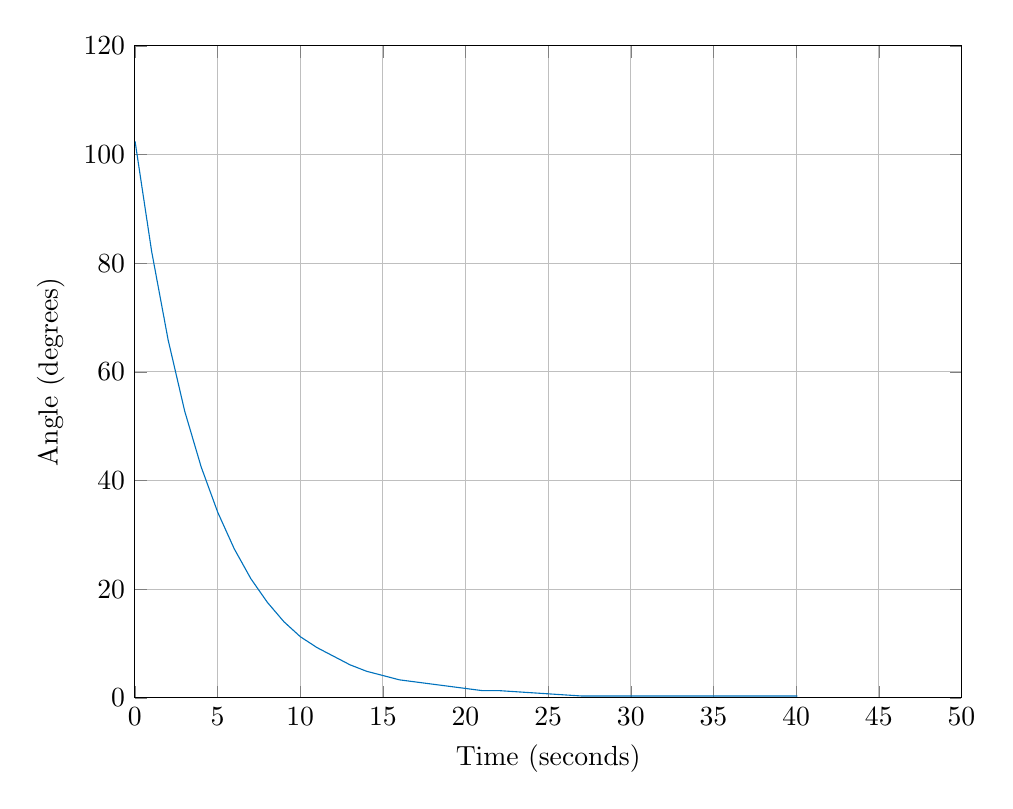
\begin{tikzpicture}

\begin{axis}[%
width=4.133in,
height=3.26in,
at={(0.693in,0.44in)},
scale only axis,
xmin=0,
xmax=50,
xmajorgrids,
xlabel={Time (seconds)},
ymin=0,
ymax=120,
ymajorgrids,
ylabel={Angle (degrees)},
axis background/.style={fill=white}
]
\addplot [color=mycolor1,solid,forget plot]
  table[row sep=crcr]{%
0	102.4204\\
0.0177441540000001	102.2904\\
0.0327040630000001	102.0084\\
0.0478449689999996	101.7024\\
0.0659545939999996	101.3764\\
0.080935841	101.0304\\
0.095923176	100.7244\\
0.11195197	100.3944\\
0.128055795	100.0804\\
0.143941748	99.7664\\
0.159967933999999	99.4424\\
0.176042313999999	99.1204\\
0.191954450999999	98.7984\\
0.208009254	98.4744\\
0.22399488	98.1384\\
0.239953013999999	97.8224\\
0.256054853999999	97.5004\\
0.272063669	97.1744\\
0.288027004	96.8584\\
0.303887813	96.5344\\
0.319971607	96.2124\\
0.335942635	95.8864\\
0.352025743	95.5644\\
0.3679568	95.2404\\
0.383953943	94.9204\\
0.399997912	94.5904\\
0.415998250999999	94.2584\\
0.431831394	93.9364\\
0.447814032000001	93.6144\\
0.463808589999999	93.2984\\
0.479903010999999	92.9684\\
0.495925008	92.6384\\
0.511948347	92.3244\\
0.528016396999999	92.0044\\
0.543863147999999	91.6824\\
0.562388751999999	91.3364\\
0.577608655	91.0044\\
0.592719001999999	90.6904\\
0.608161168000001	90.3764\\
0.624069551	90.0484\\
0.639885296999999	89.7304\\
0.655866359	89.4184\\
0.671987365999999	89.0844\\
0.68802496	88.7644\\
0.703813795999999	88.4404\\
0.719840768	88.1244\\
0.738192618	87.7884\\
0.753498854999999	87.4724\\
0.768784837	87.1484\\
0.784015643	86.8264\\
0.79988878	86.5084\\
0.815969871	86.1864\\
0.831983674	85.8584\\
0.848057242	85.5364\\
0.863854896999999	85.2164\\
0.879894759999999	84.8904\\
0.896003269	84.5704\\
0.911933238999999	84.2464\\
0.928035511999999	83.9184\\
0.943938683999999	83.5984\\
0.960191785999999	83.2744\\
0.975936873000001	82.9504\\
0.991975221	82.6244\\
1.007904933	82.2844\\
1.025398666	81.9884\\
1.040304124	81.7444\\
1.055833496	81.4964\\
1.07185873	81.2404\\
1.090013931	80.9524\\
1.10576894	80.6964\\
1.120861382	80.4444\\
1.13702896	80.1784\\
1.152233154	79.9104\\
1.167848246	79.6544\\
1.183945535	79.4024\\
1.199813575	79.1404\\
1.21810959	78.8724\\
1.233479532	78.6064\\
1.248819967	78.3504\\
1.264119629	78.0944\\
1.2799481	77.8364\\
1.29600457	77.5724\\
1.311980842	77.3024\\
1.327919031	77.0324\\
1.343886916	76.7824\\
1.362367992	76.5124\\
1.377645444	76.2584\\
1.392841231	76.0024\\
1.408078793	75.7424\\
1.424022405	75.4824\\
1.44007512	75.2244\\
1.456127821	74.9624\\
1.472010755	74.6984\\
1.488089533	74.4384\\
1.505276587	74.1684\\
1.52042763	73.9004\\
1.53601755	73.6464\\
1.551942352	73.3884\\
1.567911675	73.1324\\
1.583936325	72.8704\\
1.59989258	72.6104\\
1.615819365	72.3484\\
1.632013797	72.0864\\
1.647959463	71.8264\\
1.663988703	71.5504\\
1.679942628	71.2924\\
1.695987233	71.0364\\
1.712021079	70.7784\\
1.727901406	70.5184\\
1.743933763	70.2584\\
1.762257126	69.9884\\
1.777463037	69.7304\\
1.792770717	69.4624\\
1.808294613	69.2004\\
1.823994137	68.9484\\
1.839996003	68.6904\\
1.856026653	68.4284\\
1.87199263	68.1664\\
1.887955314	67.8964\\
1.903810895	67.6384\\
1.919953914	67.3844\\
1.937593507	67.1124\\
1.952661926	66.8484\\
1.968163942	66.5904\\
1.984178283	66.3324\\
1.999975183	66.0704\\
2.017791296	65.7864\\
2.033056711	65.5964\\
2.047987846	65.4004\\
2.063870266	65.1944\\
2.079834083	64.9804\\
2.096071024	64.7744\\
2.111796419	64.5704\\
2.128044492	64.3624\\
2.143898936	64.1504\\
2.162297373	63.9344\\
2.177444796	63.7284\\
2.192580046	63.5124\\
2.208046917	63.3064\\
2.223993811	63.1024\\
2.239942403	62.8964\\
2.255908685	62.6904\\
2.271844786	62.4784\\
2.290082946	62.2644\\
2.305663551	62.0484\\
2.321427334	61.8464\\
2.337415825	61.6344\\
2.353051482	61.4204\\
2.368230299	61.2164\\
2.384770288	61.0064\\
2.400381588	60.8004\\
2.416019773	60.5944\\
2.432075243	60.3864\\
2.447866992	60.1744\\
2.464034625	59.9684\\
2.479959588	59.7564\\
2.49605535	59.5484\\
2.511924627	59.3344\\
2.528096842	59.1224\\
2.543935965	58.9204\\
2.562280086	58.7044\\
2.577486766	58.4964\\
2.592615542	58.2884\\
2.607909968	58.0824\\
2.624013005	57.8764\\
2.639972317	57.6664\\
2.656019128	57.4564\\
2.671991098	57.2464\\
2.68783833	57.0384\\
2.70381914	56.8264\\
2.719797684	56.6184\\
2.735945271	56.4004\\
2.751977241	56.1984\\
2.767867978	55.9944\\
2.7839776	55.7844\\
2.799980396	55.5704\\
2.816165123	55.3624\\
2.832033263	55.1524\\
2.847985654	54.9444\\
2.864002992	54.7344\\
2.879987682	54.5264\\
2.895901791	54.3164\\
2.912123187	54.1064\\
2.928500747	53.8944\\
2.943946666	53.6764\\
2.959812605	53.4824\\
2.976001123	53.2704\\
2.991910687	53.0644\\
3.0078866	52.8424\\
3.024033743	52.6524\\
3.039833721	52.4944\\
3.055898507	52.3384\\
3.071898381	52.1744\\
3.088173756	52.0064\\
3.104241709	51.8384\\
3.119908618	51.6784\\
3.135877983	51.5124\\
3.151981441	51.3504\\
3.167814753	51.1824\\
3.184016414	51.0204\\
3.200035055	50.8524\\
3.215996707	50.6904\\
3.232054362	50.5204\\
3.247981445	50.3564\\
3.264166714	50.1904\\
3.279790125	50.0304\\
3.296012658	49.8644\\
3.311932396	49.7004\\
3.328156619	49.5344\\
3.343862637	49.3684\\
3.360331353	49.2044\\
3.376034386	49.0404\\
3.391958477	48.8744\\
3.407941351	48.7124\\
3.423828912	48.5464\\
3.442126699	48.3744\\
3.457365924	48.2124\\
3.472518824	48.0504\\
3.487868274	47.8844\\
3.503812755	47.7184\\
3.519945999	47.5484\\
3.536039249	47.3864\\
3.551938139	47.2284\\
3.568311326	47.0584\\
3.58398362	46.8904\\
3.599969341	46.7284\\
3.615951755	46.5644\\
3.63205545	46.4004\\
3.64796565	46.2344\\
3.665660884	46.0664\\
3.680830758	45.8984\\
3.696031371	45.7384\\
3.711993129	45.5684\\
3.728110995	45.4084\\
3.743985369	45.2424\\
3.760051875	45.0824\\
3.775931153	44.9184\\
3.792102727	44.7544\\
3.808065336	44.5884\\
3.823949485	44.4244\\
3.839914836	44.2564\\
3.856126292	44.0884\\
3.873129683	43.9244\\
3.888415745	43.7624\\
3.904082118	43.5984\\
3.919984447	43.4344\\
3.936797435	43.2664\\
3.95218989	43.0964\\
3.968030944	42.9344\\
3.983982969	42.7644\\
4.000019606	42.6004\\
4.01792116	42.4224\\
4.032913303	42.3104\\
4.047921539	42.1824\\
4.063861382	42.0524\\
4.079857392	41.9164\\
4.095891563	41.7824\\
4.111924659	41.6524\\
4.128192669	41.5204\\
4.143978449	41.3864\\
4.160134024	41.2524\\
4.175925001	41.1144\\
4.191796591	40.9824\\
4.208089832	40.8524\\
4.223946351	40.7204\\
4.239814982	40.5824\\
4.255999085	40.4524\\
4.271969471	40.3204\\
4.290295194	40.1804\\
4.305524384	40.0464\\
4.320741453	39.9204\\
4.335983263	39.7884\\
4.351886062	39.6544\\
4.368028138	39.5224\\
4.383969334	39.3824\\
4.399897934	39.2504\\
4.415925558	39.1204\\
4.431869626	38.9884\\
4.447996477	38.8524\\
4.46381962	38.7164\\
4.479957766	38.5884\\
4.495888877	38.4504\\
4.511978467	38.3144\\
4.527944261	38.1844\\
4.544003875	38.0524\\
4.560241184	37.9224\\
4.575958202	37.7904\\
4.592020126	37.6544\\
4.607920568	37.5244\\
4.624013937	37.3924\\
4.640030653	37.2584\\
4.655955594	37.1244\\
4.671990289	36.9924\\
4.688046214	36.8584\\
4.703806353	36.7224\\
4.719801313	36.5924\\
4.736013502	36.4564\\
4.751897951	36.3264\\
4.768033836	36.1924\\
4.784005832	36.0604\\
4.799899736	35.9244\\
4.815913036	35.7924\\
4.83196671	35.6584\\
4.847775381	35.5224\\
4.863984264	35.3944\\
4.879931643	35.2624\\
4.896051845	35.1244\\
4.911995762	34.9924\\
4.92815309	34.8604\\
4.94391307	34.7244\\
4.960371144	34.5904\\
4.975975883	34.4604\\
4.991936031	34.3284\\
5.00796669	34.1864\\
5.025225409	34.0624\\
5.040174419	33.9604\\
5.055830857	33.8544\\
5.071826165	33.7524\\
5.087915419	33.6364\\
5.103793775	33.5304\\
5.119982737	33.4224\\
5.13764764	33.3164\\
5.152925242	33.2104\\
5.168468381	33.0984\\
5.183880225	32.9964\\
5.199997693	32.8864\\
5.215913877	32.7764\\
5.231898023	32.6704\\
5.247995057	32.5644\\
5.2637976	32.4564\\
5.279791141	32.3464\\
5.296316409	32.2424\\
5.311987624	32.1284\\
5.328189245	32.0244\\
5.343948408	31.9164\\
5.359967983	31.8104\\
5.375954299	31.7044\\
5.391856128	31.5944\\
5.408098391	31.4864\\
5.424079379	31.3804\\
5.440023342	31.2724\\
5.456021868	31.1644\\
5.471990165	31.0544\\
5.488435392	30.9484\\
5.503975324	30.8384\\
5.519860487	30.7344\\
5.535996266	30.6244\\
5.552034071	30.5164\\
5.567791657	30.4084\\
5.583803568	30.3024\\
5.600058789	30.1884\\
5.615944598	30.0844\\
5.632002603	29.9744\\
5.647977485	29.8684\\
5.664107499	29.7604\\
5.679982405	29.6544\\
5.695809307	29.5444\\
5.711927927	29.4384\\
5.727864808	29.3324\\
5.743947707	29.2224\\
5.760158351	29.1144\\
5.775988783	29.0084\\
5.792046087	28.8964\\
5.808040178	28.7904\\
5.823975249	28.6844\\
5.839938834	28.5764\\
5.856000936	28.4684\\
5.871980058	28.3604\\
5.888114707	28.2524\\
5.903881931	28.1424\\
5.922154549	28.0324\\
5.935949996	27.9304\\
5.952079521	27.8244\\
5.967914484	27.7144\\
5.983887847	27.6044\\
6.00001967	27.4984\\
6.018431561	27.3744\\
6.033455699	27.2984\\
6.048482665	27.2164\\
6.063855193	27.1304\\
6.07987279	27.0424\\
6.095898001	26.9564\\
6.111976692	26.8724\\
6.128136278	26.7824\\
6.143940917	26.6964\\
6.159904689	26.6084\\
6.175983181	26.5184\\
6.191947174	26.4324\\
6.207838687	26.3444\\
6.224096146	26.2564\\
6.239995549	26.1684\\
6.256025953	26.0824\\
6.271936895	25.9964\\
6.2881028	25.9084\\
6.303821208	25.8204\\
6.319907718	25.7324\\
6.33602018	25.6444\\
6.351954771	25.5564\\
6.367979261	25.4684\\
6.383979535	25.3824\\
6.3999932	25.2964\\
6.415959658	25.2084\\
6.431813065	25.1204\\
6.44795526	25.0304\\
6.46633681	24.9404\\
6.481640492	24.8544\\
6.496800582	24.7684\\
6.512015123	24.6804\\
6.528007565	24.5924\\
6.544001335	24.5084\\
6.560166974	24.4204\\
6.575941672	24.3304\\
6.591818356	24.2444\\
6.607989749	24.1524\\
6.623906393	24.0664\\
6.64011637	23.9784\\
6.655979844	23.8944\\
6.673691636	23.8024\\
6.688914219	23.7144\\
6.704891777	23.6264\\
6.720183131	23.5424\\
6.737123565	23.4524\\
6.752308488	23.3684\\
6.768028357	23.2764\\
6.783980568	23.1964\\
6.799984341	23.1064\\
6.815967206	23.0164\\
6.83203869	22.9264\\
6.847972771	22.8404\\
6.864023079	22.7524\\
6.879902425	22.6664\\
6.895983262	22.5804\\
6.912068584	22.4904\\
6.928217671	22.4004\\
6.943979611	22.3184\\
6.960208831	22.2304\\
6.975958476	22.1444\\
6.992048525	22.0544\\
7.007884522	21.9604\\
7.025348728	21.8884\\
7.040294171	21.8204\\
7.055880966	21.7504\\
7.071901506	21.6824\\
7.08792888	21.6104\\
7.103913066	21.5404\\
7.120068382	21.4724\\
7.137139436	21.3984\\
7.152855242	21.3304\\
7.168165895	21.2624\\
7.183959671	21.1944\\
7.19999932	21.1264\\
7.215985663	21.0564\\
7.231883992	20.9824\\
7.247973186	20.9144\\
7.263937812	20.8464\\
7.280008721	20.7764\\
7.295851106	20.7064\\
7.312005332	20.6384\\
7.328187843	20.5684\\
7.343982595	20.4964\\
7.36024405	20.4244\\
7.375927101	20.3544\\
7.391989892	20.2844\\
7.4079011	20.2164\\
7.42401634	20.1464\\
7.440028795	20.0784\\
7.456084628	20.0064\\
7.471871999	19.9364\\
7.487989159	19.8644\\
7.504021292	19.7944\\
7.519989669	19.7284\\
7.536008014	19.6584\\
7.551949195	19.5904\\
7.567858875	19.5204\\
7.583935748	19.4484\\
7.601006903	19.3764\\
7.616333011	19.3084\\
7.631832045	19.2404\\
7.648012658	19.1724\\
7.66422105	19.1024\\
7.679991222	19.0304\\
7.695870973	18.9624\\
7.711873373	18.8924\\
7.728006439	18.8224\\
7.743939256	18.7524\\
7.76020953	18.6824\\
7.775971928	18.6104\\
7.792052602	18.5404\\
7.807974727	18.4704\\
7.823995777	18.4004\\
7.840030888	18.3344\\
7.855979139	18.2644\\
7.872011384	18.1944\\
7.8880804	18.1224\\
7.903981492	18.0544\\
7.920021161	17.9864\\
7.93706545	17.9124\\
7.952477327	17.8444\\
7.9678801	17.7764\\
7.983891723	17.7064\\
8.000016786	17.6364\\
8.017869878	17.5564\\
8.032826874	17.5104\\
8.047843233	17.4524\\
8.065963524	17.3984\\
8.080942145	17.3384\\
8.096041817	17.2824\\
8.112014951	17.2244\\
8.12803528	17.1684\\
8.14397842	17.1124\\
8.16001178	17.0544\\
8.176267969	17.0004\\
8.191914898	16.9404\\
8.207940751	16.8824\\
8.224000021	16.8284\\
8.240027206	16.7684\\
8.256005689	16.7104\\
8.272060388	16.6524\\
8.288060868	16.5984\\
8.30464051	16.5404\\
8.320066414	16.4824\\
8.335981801	16.4264\\
8.352041405	16.3684\\
8.367962458	16.3124\\
8.383991149	16.2544\\
8.399972366	16.1964\\
8.416015853	16.1384\\
8.432958448	16.0824\\
8.448360829	16.0264\\
8.463990804	15.9684\\
8.480266458	15.9124\\
8.495865174	15.8544\\
8.511956939	15.8004\\
8.527865723	15.7424\\
8.544168528	15.6844\\
8.559968157	15.6304\\
8.578390398	15.5684\\
8.593594679	15.5104\\
8.608849229	15.4604\\
8.624003037	15.4004\\
8.640080341	15.3424\\
8.655987797	15.2864\\
8.671984308	15.2284\\
8.687931107	15.1704\\
8.704159782	15.1144\\
8.719962013	15.0584\\
8.735946497	14.9984\\
8.752022388	14.9404\\
8.767927688	14.8864\\
8.783984821	14.8284\\
8.800003878	14.7724\\
8.816004223	14.7144\\
8.831966095	14.6584\\
8.848040975	14.6024\\
8.863999835	14.5424\\
8.880144963	14.4904\\
8.895806699	14.4304\\
8.912055063	14.3724\\
8.927921969	14.3124\\
8.944068836	14.2604\\
8.959911623	14.2024\\
8.978394041	14.1424\\
8.993690196	14.0844\\
9.008788051	14.0284\\
9.023814294	13.9764\\
9.041908105	13.9324\\
9.05681926	13.8904\\
9.071835365	13.8464\\
9.087841756	13.8044\\
9.103845233	13.7584\\
9.119976837	13.7104\\
9.136027025	13.6684\\
9.151993408	13.6244\\
9.167967223	13.5804\\
9.183994778	13.5344\\
9.199965717	13.4924\\
9.215891879	13.4484\\
9.231996951	13.4044\\
9.247892359	13.3584\\
9.263988631	13.3124\\
9.280002711	13.2704\\
9.295985623	13.2244\\
9.311957464	13.1804\\
9.327999411	13.1344\\
9.344179888	13.0924\\
9.360029036	13.0444\\
9.376214415	13.0024\\
9.392500602	12.9584\\
9.408018805	12.9124\\
9.423992344	12.8724\\
9.439977644	12.8244\\
9.455994021	12.7824\\
9.472021477	12.7344\\
9.488143487	12.6904\\
9.50406149	12.6444\\
9.519982771	12.6044\\
9.53603548	12.5584\\
9.552021988	12.5144\\
9.567994715	12.4724\\
9.584045985	12.4244\\
9.599980426	12.3824\\
9.616004284	12.3364\\
9.631946195	12.2924\\
9.648059476	12.2484\\
9.663985559	12.2024\\
9.679989567	12.1604\\
9.69599361	12.1144\\
9.711961915	12.0704\\
9.727990195	12.0244\\
9.744101561	11.9804\\
9.759973811	11.9364\\
9.778293465	11.8924\\
9.793577786	11.8484\\
9.808858878	11.8024\\
9.824244693	11.7624\\
9.840290734	11.7144\\
9.856116657	11.6724\\
9.872206048	11.6264\\
9.887930688	11.5824\\
9.903899309	11.5384\\
9.919951271	11.4944\\
9.935977203	11.4504\\
9.951984689	11.4044\\
9.967981481	11.3604\\
9.983956633	11.3104\\
9.999947442	11.2684\\
10.017871321	11.2244\\
10.032808961	11.1944\\
10.047859833	11.1644\\
10.063820433	11.1344\\
10.0819286	11.1004\\
10.09690558	11.0704\\
10.112008278	11.0364\\
10.127976725	11.0064\\
10.144209833	10.9744\\
10.159980776	10.9444\\
10.176072019	10.9124\\
10.192019298	10.8824\\
10.207919569	10.8504\\
10.223870053	10.8184\\
10.239996002	10.7844\\
10.25602208	10.7544\\
10.272043914	10.7224\\
10.28804911	10.6924\\
10.304009835	10.6604\\
10.319993903	10.6244\\
10.336057205	10.5944\\
10.352030243	10.5644\\
10.367956325	10.5324\\
10.384016425	10.5024\\
10.399949676	10.4704\\
10.415887273	10.4384\\
10.431963201	10.4044\\
10.448001658	10.3744\\
10.46402966	10.3404\\
10.480015026	10.3104\\
10.495952148	10.2764\\
10.511976326	10.2444\\
10.5279805	10.2144\\
10.544210234	10.1824\\
10.559986281	10.1504\\
10.575948973	10.1204\\
10.591905897	10.0884\\
10.608046685	10.0544\\
10.623974856	10.0244\\
10.639982006	9.99440000000001\\
10.656007648	9.9624\\
10.672016717	9.93040000000001\\
10.688027015	9.8984\\
10.703883115	9.86439999999999\\
10.719850408	9.8344\\
10.736036028	9.80439999999999\\
10.751966715	9.77239999999999\\
10.768060426	9.7424\\
10.784009615	9.7064\\
10.799861772	9.67439999999999\\
10.815977265	9.64439999999999\\
10.832009553	9.61239999999999\\
10.847977785	9.58240000000001\\
10.864036139	9.5504\\
10.88002107	9.5184\\
10.896019403	9.48439999999999\\
10.911838149	9.45039999999999\\
10.927964589	9.41839999999999\\
10.944132473	9.38839999999999\\
10.960012842	9.35639999999999\\
10.97599494	9.32640000000001\\
10.991880004	9.2944\\
11.007970899	9.26239999999999\\
11.025414481	9.23239999999998\\
11.040451894	9.2084\\
11.055869466	9.18640000000001\\
11.071919421	9.16040000000001\\
11.087924862	9.1344\\
11.103969424	9.1024\\
11.1199788	9.07639999999999\\
11.135877788	9.0504\\
11.151980131	9.02640000000001\\
11.167941124	9.00039999999998\\
11.183995078	8.97639999999998\\
11.200015884	8.95239999999998\\
11.215937089	8.9264\\
11.232019305	8.90040000000002\\
11.248020617	8.87639999999999\\
11.26421936	8.8484\\
11.280012	8.8244\\
11.296021746	8.79639999999999\\
11.312080644	8.77440000000001\\
11.328057691	8.74639999999999\\
11.344028408	8.72439999999999\\
11.360011019	8.69639999999998\\
11.376003706	8.6704\\
11.391936738	8.6464\\
11.407981734	8.62039999999999\\
11.424002395	8.59639999999999\\
11.440014917	8.57039999999999\\
11.45609619	8.54639999999999\\
11.472070065	8.5204\\
11.488103465	8.4944\\
11.5039031	8.4704\\
11.520077922	8.44439999999999\\
11.536003773	8.4164\\
11.551989733	8.39439999999999\\
11.567961579	8.3664\\
11.584026304	8.3424\\
11.599964638	8.31639999999999\\
11.615866219	8.2924\\
11.632051283	8.2664\\
11.648008565	8.24039999999999\\
11.663991783	8.21639999999999\\
11.679955904	8.19039999999998\\
11.695908896	8.1664\\
11.712044954	8.14039999999999\\
11.727984646	8.1144\\
11.744266289	8.09039999999997\\
11.760126251	8.06439999999999\\
11.7760434	8.0364\\
11.792132146	8.01439999999999\\
11.808050886	7.9864\\
11.823997807	7.9624\\
11.84004679	7.93639999999999\\
11.855996079	7.91040000000001\\
11.872030726	7.88639999999998\\
11.888012132	7.8604\\
11.90389773	7.83639999999998\\
11.919992051	7.80839999999999\\
11.935992807	7.78440000000001\\
11.95189877	7.75839999999998\\
11.967868711	7.7324\\
11.984037355	7.70639999999999\\
12.000105929	7.68039999999999\\
12.017849286	7.65440000000001\\
12.032768543	7.63239999999999\\
12.047866061	7.60639999999999\\
12.063880419	7.58039999999998\\
12.079877976	7.5564\\
12.098046519	7.5284\\
12.113407982	7.50639999999999\\
12.128578276	7.47839999999999\\
12.14398879	7.45439999999999\\
12.159980736	7.43039999999999\\
12.176133999	7.40440000000001\\
12.191915091	7.37639999999999\\
12.208001663	7.3544\\
12.224002396	7.32639999999999\\
12.239964929	7.30239999999999\\
12.255964619	7.27640000000001\\
12.272018179	7.25039999999998\\
12.287907709	7.22639999999998\\
12.303960852	7.20039999999999\\
12.319980397	7.1764\\
12.335941135	7.1484\\
12.351983059	7.12439999999999\\
12.367987037	7.0984\\
12.384113476	7.0744\\
12.400041719	7.04639999999999\\
12.416061042	7.02440000000001\\
12.431941691	6.99639999999999\\
12.447990776	6.97239999999999\\
12.46400612	6.94639999999998\\
12.47986539	6.9224\\
12.496005331	6.8964\\
12.511977477	6.8724\\
12.527990866	6.84639999999999\\
12.544075412	6.82039999999999\\
12.560051507	6.79639999999999\\
12.576208672	6.7704\\
12.591987399	6.7444\\
12.607988185	6.7204\\
12.623998292	6.69439999999999\\
12.640042872	6.6664\\
12.655954371	6.64439999999999\\
12.671993002	6.6144\\
12.688069214	6.5924\\
12.704052035	6.56439999999999\\
12.720157683	6.5424\\
12.735883019	6.5164\\
12.751988071	6.49039999999999\\
12.767953513	6.46639999999999\\
12.784022603	6.44039999999998\\
12.79994475	6.4144\\
12.815851826	6.39039999999999\\
12.831979317	6.3644\\
12.848006828	6.33639999999998\\
12.864024507	6.3124\\
12.879993846	6.2864\\
12.896013505	6.26039999999999\\
12.912028027	6.2364\\
12.927939231	6.2124\\
12.94406223	6.18639999999999\\
12.959992479	6.16040000000001\\
12.978385834	6.13639999999998\\
12.993673517	6.10839999999999\\
13.008884356	6.08039999999998\\
13.023873171	6.0624\\
13.039965823	6.0424\\
13.055962863	6.02440000000001\\
13.072056005	6.00839999999999\\
13.088051354	5.99039999999999\\
13.103908324	5.9704\\
13.119826742	5.94839999999999\\
13.135977399	5.93039999999999\\
13.151916194	5.91240000000001\\
13.168070177	5.89239999999998\\
13.18398576	5.8724\\
13.199890941	5.8524\\
13.215990689	5.83439999999999\\
13.231990683	5.81439999999999\\
13.248005491	5.8004\\
13.263988195	5.78040000000001\\
13.280023099	5.76039999999999\\
13.295914622	5.74039999999999\\
13.3120289	5.72239999999999\\
13.327973192	5.70239999999998\\
13.3463917	5.68039999999999\\
13.361635521	5.66240000000001\\
13.376936742	5.64239999999998\\
13.392542949	5.62439999999999\\
13.407984984	5.60839999999999\\
13.423990415	5.58839999999998\\
13.440035161	5.57039999999999\\
13.456027312	5.5504\\
13.472029757	5.53240000000001\\
13.488019035	5.51239999999999\\
13.504048668	5.4924\\
13.519997101	5.47239999999999\\
13.535957424	5.45239999999998\\
13.551978436	5.4344\\
13.567960935	5.4204\\
13.583982097	5.40040000000002\\
13.600088893	5.38039999999998\\
13.616051723	5.3604\\
13.632095198	5.3404\\
13.647936911	5.32239999999999\\
13.664018976	5.30239999999999\\
13.679929405	5.28240000000001\\
13.696115557	5.26239999999999\\
13.712088791	5.2444\\
13.728079724	5.22439999999999\\
13.744146188	5.21040000000001\\
13.760004076	5.19039999999998\\
13.776138129	5.1704\\
13.791990433	5.15040000000002\\
13.808319523	5.13239999999999\\
13.823991519	5.11239999999999\\
13.840876282	5.0924\\
13.856198395	5.07239999999999\\
13.872022927	5.0544\\
13.88799893	5.0364\\
13.903902853	5.01839999999999\\
13.920299171	5.00039999999998\\
13.936524143	4.9804\\
13.952003133	4.96040000000001\\
13.967922164	4.94239999999999\\
13.984021356	4.9224\\
14.000004302	4.90240000000001\\
14.021512803	4.88239999999999\\
14.033500279	4.8724\\
14.048825728	4.8604\\
14.064094519	4.8484\\
14.079982062	4.8344\\
14.096036069	4.8244\\
14.111978945	4.81039999999999\\
14.127970598	4.79639999999999\\
14.144272802	4.78440000000001\\
14.159927968	4.77239999999999\\
14.176001765	4.76039999999999\\
14.191993996	4.74839999999999\\
14.208044255	4.73439999999999\\
14.224030353	4.7204\\
14.239899612	4.71040000000001\\
14.25595932	4.6964\\
14.271973075	4.6844\\
14.28807093	4.6704\\
14.303881156	4.66040000000001\\
14.319956078	4.64439999999999\\
14.337491235	4.63239999999999\\
14.352804817	4.62039999999999\\
14.368146496	4.60839999999999\\
14.384045512	4.59439999999999\\
14.399862218	4.58239999999998\\
14.415813551	4.57039999999999\\
14.431962165	4.55839999999999\\
14.447932542	4.5444\\
14.464199591	4.53040000000001\\
14.47987596	4.5204\\
14.496005858	4.5044\\
14.511931121	4.4944\\
14.527984224	4.4804\\
14.543959983	4.4684\\
14.559920262	4.45439999999999\\
14.576162621	4.44239999999999\\
14.591981038	4.43039999999999\\
14.608046856	4.41839999999999\\
14.62399606	4.40440000000001\\
14.640035955	4.39039999999999\\
14.655874969	4.38039999999998\\
14.67200585	4.3664\\
14.687913297	4.3544\\
14.703887227	4.3404\\
14.720035739	4.33039999999998\\
14.736084322	4.31440000000001\\
14.751996589	4.30439999999999\\
14.767982716	4.29040000000001\\
14.784021955	4.2784\\
14.799951995	4.26439999999999\\
14.815974284	4.25239999999999\\
14.832722157	4.24039999999999\\
14.848035872	4.22839999999999\\
14.86398905	4.2144\\
14.880026604	4.20039999999999\\
14.896024939	4.19039999999998\\
14.912215675	4.1764\\
14.927989651	4.1644\\
14.943997957	4.15040000000002\\
14.959906851	4.14039999999999\\
14.978305886	4.12439999999999\\
14.99354199	4.11239999999999\\
15.008697568	4.0984\\
15.023974395	4.0844\\
15.039986789	4.0744\\
15.056140917	4.06039999999999\\
15.072027932	4.0504\\
15.087898911	4.0384\\
15.104072529	4.02439999999999\\
15.119999799	4.01039999999999\\
15.136014341	4.00039999999998\\
15.151948685	3.98439999999999\\
15.16794009	3.97439999999999\\
15.183979463	3.96040000000001\\
15.200022249	3.94839999999999\\
15.215902045	3.9344\\
15.231979085	3.9224\\
15.24810982	3.9084\\
15.26400462	3.89840000000001\\
15.279983627	3.8844\\
15.296015789	3.87039999999999\\
15.311988997	3.8604\\
15.327958147	3.84639999999999\\
15.344116503	3.8344\\
15.359944198	3.81839999999998\\
15.375985619	3.8064\\
15.391964544	3.79040000000001\\
15.407926139	3.78040000000001\\
15.423929022	3.7684\\
15.440027877	3.75439999999999\\
15.4559316	3.74039999999999\\
15.471922784	3.7304\\
15.487959992	3.71639999999999\\
15.503849215	3.70439999999999\\
15.522218674	3.68839999999999\\
15.537355028	3.6784\\
15.552485878	3.6664\\
15.567856399	3.65240000000001\\
15.583983553	3.64039999999999\\
15.599907845	3.62839999999998\\
15.615964183	3.6164\\
15.631958534	3.60040000000001\\
15.64799247	3.59039999999997\\
15.663977415	3.57839999999999\\
15.679929334	3.56439999999999\\
15.695828736	3.5504\\
15.712003932	3.54040000000001\\
15.72812514	3.52640000000001\\
15.744129129	3.51239999999999\\
15.759839239	3.50039999999998\\
15.776051962	3.4884\\
15.791962243	3.4764\\
15.807942971	3.46039999999998\\
15.824014363	3.45039999999999\\
15.840027182	3.43839999999999\\
15.855982539	3.42440000000001\\
15.872008117	3.41040000000001\\
15.887972795	3.40040000000002\\
15.903826785	3.38839999999998\\
15.919920663	3.3724\\
15.935967355	3.3604\\
15.95200946	3.3484\\
15.967943705	3.33639999999998\\
15.983972538	3.32239999999999\\
15.999983157	3.3124\\
16.018615015	3.29839999999999\\
16.031993003	3.29639999999999\\
16.048060554	3.2884\\
16.064007484	3.28240000000001\\
16.079901392	3.2784\\
16.095854435	3.2704\\
16.111999047	3.26239999999999\\
16.128037352	3.25839999999999\\
16.144240554	3.25039999999998\\
16.159954101	3.2424\\
16.175951184	3.2384\\
16.191984654	3.2324\\
16.207904056	3.2264\\
16.223985031	3.2204\\
16.240024681	3.2124\\
16.25600208	3.2084\\
16.272006995	3.20039999999999\\
16.288044368	3.19239999999999\\
16.304065686	3.18839999999999\\
16.319995551	3.18039999999999\\
16.335958025	3.1724\\
16.352009455	3.16839999999999\\
16.367880078	3.16240000000001\\
16.38399931	3.1584\\
16.399958407	3.15040000000002\\
16.415849514	3.14239999999998\\
16.431883881	3.13839999999999\\
16.447992115	3.13039999999998\\
16.464002217	3.1224\\
16.480128507	3.11839999999999\\
16.495935629	3.1104\\
16.511965451	3.10639999999999\\
16.527942849	3.0984\\
16.544002784	3.0924\\
16.559951852	3.08840000000001\\
16.576310388	3.08039999999998\\
16.591993916	3.07239999999999\\
16.607981093	3.0684\\
16.624099508	3.06039999999999\\
16.639977816	3.05239999999999\\
16.655957981	3.04839999999999\\
16.672075781	3.0424\\
16.687981617	3.0364\\
16.70408034	3.03040000000001\\
16.720016419	3.02239999999999\\
16.7359338	3.01839999999999\\
16.752928353	3.01039999999999\\
16.768076001	3.00239999999999\\
16.784042128	2.99839999999999\\
16.799941782	2.99039999999999\\
16.816403911	2.98440000000001\\
16.831945972	2.97839999999999\\
16.848033424	2.97239999999999\\
16.86404063	2.96639999999999\\
16.880056043	2.96040000000001\\
16.89597555	2.95239999999998\\
16.911809413	2.94839999999999\\
16.927964491	2.94039999999998\\
16.943859189	2.9324\\
16.959847547	2.9284\\
16.976306144	2.9204\\
16.991895648	2.9144\\
17.007861192	2.9084\\
17.023903461	2.90240000000001\\
17.039888521	2.8964\\
17.055981314	2.89039999999999\\
17.071804681	2.88239999999999\\
17.08812132	2.87839999999998\\
17.103986067	2.87039999999999\\
17.11994946	2.86239999999999\\
17.135943308	2.85839999999999\\
17.152028495	2.8524\\
17.167997112	2.84439999999999\\
17.183813738	2.8404\\
17.1999706	2.83239999999998\\
17.216001494	2.82839999999999\\
17.231945523	2.82039999999999\\
17.248143254	2.8124\\
17.263959356	2.80839999999999\\
17.279957697	2.8004\\
17.295903573	2.7924\\
17.311831899	2.7884\\
17.327913376	2.78240000000001\\
17.34387256	2.7764\\
17.360021005	2.7704\\
17.376265783	2.76239999999999\\
17.392021055	2.75839999999999\\
17.407958846	2.75039999999998\\
17.424052004	2.7424\\
17.440041537	2.7384\\
17.455980248	2.7304\\
17.47205077	2.72239999999999\\
17.487902924	2.7184\\
17.503972557	2.7124\\
17.519909292	2.7064\\
17.535974259	2.70039999999999\\
17.551906023	2.69239999999999\\
17.567973181	2.68839999999999\\
17.583989841	2.68039999999999\\
17.599989014	2.6724\\
17.615818706	2.66839999999999\\
17.631799887	2.66040000000001\\
17.64796211	2.65240000000001\\
17.66402742	2.64840000000001\\
17.680030102	2.64239999999998\\
17.695854282	2.63839999999999\\
17.711905321	2.63039999999998\\
17.727900065	2.6224\\
17.744114573	2.61839999999999\\
17.75999217	2.6104\\
17.776111038	2.6024\\
17.791797316	2.5984\\
17.808062441	2.5924\\
17.823913438	2.58439999999999\\
17.840021682	2.58039999999998\\
17.855995502	2.57239999999999\\
17.872057927	2.5684\\
17.88793406	2.56039999999999\\
17.90402632	2.55239999999999\\
17.919969605	2.54839999999999\\
17.936015152	2.54040000000001\\
17.952047514	2.53240000000001\\
17.967998953	2.5284\\
17.98408643	2.5204\\
17.999937903	2.51439999999999\\
18.017713904	2.51039999999999\\
18.032926989	2.50239999999999\\
18.048076682	2.49839999999999\\
18.063924107	2.49039999999999\\
18.080003085	2.4824\\
18.096008291	2.47839999999999\\
18.111842246	2.4704\\
18.130062683	2.4624\\
18.145491549	2.4584\\
18.160759238	2.45039999999999\\
18.175956101	2.4464\\
18.191884821	2.43839999999999\\
18.20806147	2.4324\\
18.224692697	2.4284\\
18.239952728	2.4204\\
18.256008258	2.41240000000001\\
18.272024733	2.4084\\
18.288010349	2.40040000000002\\
18.30410588	2.39239999999998\\
18.320001355	2.38839999999999\\
18.335972967	2.38239999999999\\
18.351979796	2.37839999999998\\
18.36816057	2.37039999999999\\
18.383868069	2.36239999999999\\
18.400025477	2.35839999999999\\
18.416136989	2.35040000000001\\
18.431947889	2.3424\\
18.447949276	2.33840000000001\\
18.463946043	2.33239999999998\\
18.479997801	2.32639999999999\\
18.496050152	2.32039999999999\\
18.511806667	2.3124\\
18.527798792	2.30639999999998\\
18.543893029	2.3004\\
18.559880903	2.2924\\
18.576054051	2.2884\\
18.591822555	2.28040000000001\\
18.607864675	2.27239999999999\\
18.623982842	2.26839999999999\\
18.640034433	2.26239999999999\\
18.655940578	2.2564\\
18.671970701	2.24839999999999\\
18.688088237	2.2424\\
18.704055742	2.2384\\
18.719847187	2.2304\\
18.735947129	2.22239999999999\\
18.751992392	2.2184\\
18.767902927	2.21040000000001\\
18.783831042	2.20239999999998\\
18.7999934	2.19839999999999\\
18.815810661	2.19239999999999\\
18.834114914	2.18639999999999\\
18.84946709	2.18039999999999\\
18.864867929	2.1724\\
18.880255113	2.16839999999999\\
18.895962589	2.16040000000001\\
18.911859012	2.15240000000001\\
18.927977997	2.14840000000001\\
18.943940977	2.14039999999999\\
18.959923903	2.13439999999999\\
18.976041518	2.12839999999998\\
18.991981506	2.1224\\
19.007935539	2.1164\\
19.025572889	2.10839999999999\\
19.040871928	2.1024\\
19.056438628	2.0984\\
19.072266862	2.0904\\
19.087987123	2.08239999999998\\
19.104017448	2.07839999999999\\
19.120041113	2.07039999999999\\
19.136089582	2.06439999999999\\
19.152001241	2.05839999999999\\
19.167970653	2.05239999999999\\
19.183993411	2.04839999999999\\
19.19997326	2.04040000000001\\
19.217370569	2.03240000000001\\
19.232709265	2.0284\\
19.248086704	2.0204\\
19.263974539	2.01239999999999\\
19.280053441	2.00839999999999\\
19.295960011	2.00239999999999\\
19.311846466	1.99639999999999\\
19.330104587	1.99039999999999\\
19.345462389	1.9824\\
19.36091123	1.97839999999999\\
19.376104842	1.9704\\
19.391941061	1.9624\\
19.407895005	1.9584\\
19.424153682	1.95039999999999\\
19.439978196	1.94239999999999\\
19.455975314	1.93839999999999\\
19.472029896	1.9324\\
19.487922857	1.92639999999999\\
19.50403235	1.9204\\
19.519984596	1.91240000000001\\
19.536018948	1.9084\\
19.552021052	1.90040000000002\\
19.567933364	1.89239999999998\\
19.584057507	1.88839999999999\\
19.599982401	1.88039999999998\\
19.616378024	1.8724\\
19.631959547	1.86839999999999\\
19.647867944	1.86239999999999\\
19.663884525	1.85839999999999\\
19.680028676	1.85040000000001\\
19.69598001	1.8424\\
19.711797359	1.83840000000001\\
19.729901931	1.83039999999998\\
19.745080392	1.82239999999999\\
19.760194592	1.8184\\
19.77598209	1.81039999999999\\
19.791910871	1.80639999999998\\
19.808114813	1.8004\\
19.823910719	1.7924\\
19.839977941	1.7884\\
19.856102042	1.78040000000001\\
19.872069051	1.77239999999999\\
19.887886331	1.76839999999999\\
19.904063416	1.76039999999999\\
19.919879187	1.75239999999999\\
19.935990063	1.74839999999999\\
19.952153276	1.74039999999999\\
19.967911568	1.7364\\
19.984041665	1.72839999999999\\
19.999969177	1.72239999999999\\
20.017754685	1.71639999999999\\
20.033065576	1.71040000000001\\
20.048261028	1.70239999999998\\
20.065148395	1.69839999999999\\
20.080584776	1.69039999999998\\
20.095921297	1.6824\\
20.112314658	1.6784\\
20.128072212	1.6724\\
20.144050322	1.6644\\
20.160008674	1.66040000000001\\
20.176244886	1.65240000000001\\
20.191946088	1.64840000000001\\
20.208192053	1.64039999999999\\
20.223937571	1.63239999999999\\
20.240101997	1.62839999999998\\
20.255949027	1.62039999999999\\
20.272073862	1.6144\\
20.288048639	1.60839999999999\\
20.303961711	1.6024\\
20.320062529	1.5984\\
20.336051327	1.5904\\
20.351867158	1.58239999999998\\
20.367998558	1.57839999999999\\
20.384235131	1.57039999999999\\
20.399970861	1.5624\\
20.416047321	1.55839999999999\\
20.432002035	1.5504\\
20.447985038	1.5444\\
20.463823328	1.5384\\
20.479886681	1.53240000000001\\
20.495986982	1.5284\\
20.511926494	1.5204\\
20.527922729	1.51239999999999\\
20.543957572	1.50839999999999\\
20.559990106	1.50039999999998\\
20.575967763	1.4924\\
20.592058742	1.4884\\
20.60784029	1.4824\\
20.623964623	1.4764\\
20.639915171	1.4684\\
20.655942033	1.4624\\
20.672022121	1.4584\\
20.687986574	1.45039999999999\\
20.707530295	1.44239999999999\\
20.7198142	1.43839999999999\\
20.735799943	1.43039999999999\\
20.754076883	1.4224\\
20.769131774	1.41839999999999\\
20.785242884	1.41040000000001\\
20.800413404	1.4064\\
20.815900959	1.40040000000002\\
20.831911751	1.39239999999998\\
20.847991349	1.38839999999999\\
20.864215246	1.38039999999998\\
20.880172489	1.3724\\
20.89604119	1.36839999999999\\
20.912091578	1.3604\\
20.927945847	1.3544\\
20.944081173	1.3484\\
20.960066684	1.3424\\
20.975969002	1.33840000000001\\
20.991931671	1.33039999999998\\
21.007976778	1.3244\\
21.025607157	1.32239999999999\\
21.041084259	1.32239999999999\\
21.056381035	1.32239999999999\\
21.071975516	1.32239999999999\\
21.08800851	1.32239999999999\\
21.104036106	1.32239999999999\\
21.11978888	1.32239999999999\\
21.136058816	1.32239999999999\\
21.151994684	1.32239999999999\\
21.167953509	1.32239999999999\\
21.184001052	1.32239999999999\\
21.199977548	1.32239999999999\\
21.215797052	1.32239999999999\\
21.234055508	1.32239999999999\\
21.249365023	1.32239999999999\\
21.264517231	1.32239999999999\\
21.280016451	1.32239999999999\\
21.295960836	1.32239999999999\\
21.311862378	1.32239999999999\\
21.327983413	1.32239999999999\\
21.34406115	1.32239999999999\\
21.359918185	1.32239999999999\\
21.375870588	1.32239999999999\\
21.391958276	1.32239999999999\\
21.408024456	1.32239999999999\\
21.423858845	1.32239999999999\\
21.439904702	1.32239999999999\\
21.455890771	1.32239999999999\\
21.472065636	1.32239999999999\\
21.487990324	1.32239999999999\\
21.503924697	1.32239999999999\\
21.519952902	1.32239999999999\\
21.536053434	1.32239999999999\\
21.552156546	1.32239999999999\\
21.567988841	1.32239999999999\\
21.583994477	1.32239999999999\\
21.59996743	1.32239999999999\\
21.615992246	1.32239999999999\\
21.655064028	1.32239999999999\\
21.670173849	1.32239999999999\\
21.686191848	1.32239999999999\\
21.702176256	1.32239999999999\\
21.718242571	1.32239999999999\\
21.734196731	1.32239999999999\\
21.752411665	1.32239999999999\\
21.767800269	1.32239999999999\\
21.783079991	1.32239999999999\\
21.798362695	1.32239999999999\\
21.814357483	1.32239999999999\\
21.830303609	1.32239999999999\\
21.846278672	1.32239999999999\\
21.862192804	1.32239999999999\\
21.880667552	1.32239999999999\\
21.895776652	1.32239999999999\\
21.910926669	1.32239999999999\\
21.926283994	1.32239999999999\\
21.944665708	1.32239999999999\\
21.959741178	1.32239999999999\\
21.974922207	1.32239999999999\\
21.990247147	1.32239999999999\\
22.006397717	1.32239999999999\\
22.023988324	1.32239999999999\\
22.039055139	1.32039999999999\\
22.05430491	1.3164\\
22.070331314	1.31440000000001\\
22.086381205	1.3124\\
22.102324425	1.30839999999999\\
22.11844384	1.30439999999999\\
22.134320397	1.30239999999999\\
22.150300566	1.29839999999999\\
22.166279265	1.2944\\
22.182322897	1.2924\\
22.198249003	1.2884\\
22.214245136	1.28440000000001\\
22.230301005	1.28240000000001\\
22.246394786	1.2784\\
22.262230523	1.27439999999999\\
22.278448973	1.27239999999999\\
22.294239367	1.26839999999999\\
22.310426027	1.26639999999999\\
22.326201298	1.26239999999999\\
22.342466703	1.26039999999999\\
22.358312833	1.2564\\
22.374320144	1.2544\\
22.390375329	1.25239999999999\\
22.406225986	1.24639999999999\\
22.422235792	1.2444\\
22.438465649	1.2424\\
22.454329415	1.2384\\
22.470383371	1.23439999999999\\
22.486352676	1.2324\\
22.502240175	1.22839999999999\\
22.518396709	1.2244\\
22.534244035	1.22239999999999\\
22.550249363	1.2184\\
22.566291798	1.2144\\
22.582415262	1.2124\\
22.5984103	1.2084\\
22.614325262	1.20439999999999\\
22.630270806	1.20239999999998\\
22.64632788	1.20239999999998\\
22.662287485	1.1964\\
22.680877012	1.1944\\
22.696397841	1.19239999999999\\
22.711552355	1.18639999999999\\
22.726574298	1.1844\\
22.742327242	1.1824\\
22.758279839	1.1784\\
22.774478613	1.17439999999999\\
22.790305551	1.1724\\
22.806395373	1.16839999999999\\
22.822354675	1.1644\\
22.838466497	1.16240000000001\\
22.854355785	1.1584\\
22.870407877	1.15440000000001\\
22.88631445	1.15240000000001\\
22.902387617	1.14840000000001\\
22.918459556	1.14439999999999\\
22.934269089	1.14239999999998\\
22.950361492	1.13839999999999\\
22.96629014	1.13639999999999\\
22.982346792	1.1344\\
22.998236221	1.13239999999999\\
23.019628587	1.12639999999999\\
23.031469793	1.12439999999999\\
23.046564953	1.1224\\
23.062298764	1.1164\\
23.078402653	1.1144\\
23.094178311	1.11239999999999\\
23.110200395	1.10839999999999\\
23.127454235	1.1044\\
23.143406326	1.1024\\
23.158732463	1.0984\\
23.174360877	1.09439999999999\\
23.190324647	1.0924\\
23.206298972	1.08840000000001\\
23.222169591	1.0844\\
23.238559523	1.08240000000001\\
23.254371491	1.07839999999999\\
23.270249796	1.0744\\
23.286372482	1.07239999999999\\
23.302282086	1.07239999999999\\
23.318186828	1.0664\\
23.334156421	1.06440000000001\\
23.350343948	1.0624\\
23.366284072	1.0564\\
23.382328887	1.05439999999999\\
23.398255897	1.05239999999999\\
23.414166942	1.04839999999999\\
23.430330648	1.0444\\
23.446383868	1.0424\\
23.462191018	1.0384\\
23.478430311	1.03440000000001\\
23.494241708	1.03240000000001\\
23.510470816	1.0284\\
23.526358042	1.02439999999999\\
23.542700745	1.02239999999999\\
23.558199073	1.01839999999999\\
23.574375386	1.01439999999999\\
23.590330593	1.01239999999999\\
23.606500598	1.00839999999999\\
23.622688537	1.0064\\
23.638185474	1.00239999999999\\
23.654196095	1.00239999999999\\
23.670408415	0.996399999999994\\
23.686326759	0.994399999999999\\
23.702264482	0.992400000000004\\
23.718290795	0.986400000000003\\
23.734374509	0.984399999999994\\
23.750286653	0.982399999999998\\
23.766291469	0.978399999999993\\
23.78234744	0.974400000000003\\
23.798177011	0.972399999999993\\
23.814320352	0.968400000000003\\
23.830228216	0.964399999999998\\
23.846288473	0.962400000000002\\
23.862190859	0.958399999999997\\
23.878302401	0.954399999999993\\
23.894256324	0.952399999999983\\
23.910209326	0.948399999999992\\
23.928327762	0.946399999999997\\
23.943538498	0.942399999999992\\
23.958722043	0.940399999999997\\
23.974378754	0.936399999999992\\
23.990177182	0.932400000000001\\
24.00855221	0.932400000000001\\
24.022871924	0.926399999999987\\
24.038509697	0.924399999999991\\
24.054292439	0.922399999999996\\
24.070268278	0.918399999999991\\
24.086144764	0.914400000000001\\
24.102335473	0.912400000000005\\
24.118289543	0.9084\\
24.134209088	0.90440000000001\\
24.150364932	0.902400000000014\\
24.16630243	0.898400000000009\\
24.18243555	0.89439999999999\\
24.198321486	0.892399999999981\\
24.214354372	0.88839999999999\\
24.230180066	0.884399999999999\\
24.246290664	0.88239999999999\\
24.262274475	0.878399999999985\\
24.278342243	0.87639999999999\\
24.294426776	0.874399999999994\\
24.310343148	0.872399999999999\\
24.326225234	0.866399999999999\\
24.342217303	0.864400000000003\\
24.360546942	0.862399999999994\\
24.375647749	0.856399999999994\\
24.390990519	0.854399999999998\\
24.406294182	0.852400000000003\\
24.422268531	0.848399999999998\\
24.438308004	0.844399999999993\\
24.454332951	0.842399999999998\\
24.470233269	0.838400000000007\\
24.486268323	0.834400000000002\\
24.502342485	0.832400000000007\\
24.518159415	0.828399999999988\\
24.534170077	0.824399999999997\\
24.550332823	0.822399999999988\\
24.56636199	0.818399999999997\\
24.582348102	0.816400000000002\\
24.598328392	0.812399999999997\\
24.61425054	0.812399999999997\\
24.630282536	0.806399999999996\\
24.646314333	0.804399999999987\\
24.66241766	0.802399999999992\\
24.678344394	0.796399999999991\\
24.69437882	0.794399999999996\\
24.710248503	0.792400000000001\\
24.726220501	0.788399999999996\\
24.742386991	0.784400000000005\\
24.758171706	0.78240000000001\\
24.774276598	0.778400000000005\\
24.790359155	0.774399999999986\\
24.806220989	0.77239999999999\\
24.822354658	0.768399999999986\\
24.838330041	0.764399999999995\\
24.854223247	0.762399999999985\\
24.870422163	0.758399999999995\\
24.886866671	0.754400000000004\\
24.902317714	0.752399999999994\\
24.918228638	0.74839999999999\\
24.934330968	0.746399999999994\\
24.950296628	0.742400000000004\\
24.966439927	0.742400000000004\\
24.982181905	0.736400000000003\\
24.998338685	0.734399999999994\\
25.019140482	0.732399999999998\\
25.031151038	0.726399999999998\\
25.04632837	0.724400000000003\\
25.062254328	0.722399999999993\\
25.07828592	0.718400000000003\\
25.094461408	0.714399999999998\\
25.110176998	0.712400000000002\\
25.126163718	0.708399999999997\\
25.142242643	0.704399999999993\\
25.158240413	0.702399999999983\\
25.174292944	0.698399999999992\\
25.19017162	0.694400000000002\\
25.206191876	0.692399999999992\\
25.222269787	0.688399999999987\\
25.238238855	0.684399999999997\\
25.256529852	0.682400000000001\\
25.272086529	0.680399999999992\\
25.28706972	0.676399999999987\\
25.302328479	0.674399999999991\\
25.318327917	0.672399999999996\\
25.334252533	0.666399999999996\\
25.350385947	0.664400000000001\\
25.366357627	0.662400000000005\\
25.382352689	0.656400000000005\\
25.398467113	0.65440000000001\\
25.414221319	0.652400000000014\\
25.430408024	0.648400000000009\\
25.446212433	0.64439999999999\\
25.464439046	0.642399999999981\\
25.479621267	0.63839999999999\\
25.49472912	0.634399999999999\\
25.510384383	0.63239999999999\\
25.526536748	0.628399999999985\\
25.542392689	0.624399999999994\\
25.558391582	0.622399999999999\\
25.574182136	0.618399999999994\\
25.590396774	0.616399999999999\\
25.606315667	0.612399999999994\\
25.622186452	0.612399999999994\\
25.638168271	0.606399999999994\\
25.654182391	0.604399999999998\\
25.670203463	0.602400000000003\\
25.686304702	0.596399999999988\\
25.702142729	0.594399999999993\\
25.720392975	0.592399999999998\\
25.735504011	0.586399999999998\\
25.750497624	0.584400000000002\\
25.766330907	0.582400000000007\\
25.782142986	0.578399999999988\\
25.800180284	0.574399999999997\\
25.815242579	0.572399999999988\\
25.830473416	0.568399999999997\\
25.846232104	0.564400000000006\\
25.862354178	0.562399999999997\\
25.878265906	0.558399999999992\\
25.894347376	0.556399999999996\\
25.91036042	0.552399999999992\\
25.926333271	0.550399999999996\\
25.942327844	0.546399999999991\\
25.958210236	0.544399999999996\\
25.976436178	0.542400000000001\\
25.991580363	0.5364\\
26.006959245	0.534400000000005\\
26.024235248	0.53240000000001\\
26.039267488	0.52640000000001\\
26.054277042	0.524399999999986\\
26.070167825	0.52239999999999\\
26.086260823	0.518399999999986\\
26.102151778	0.514399999999995\\
26.118181712	0.512399999999985\\
26.13432692	0.508399999999995\\
26.150200076	0.504400000000004\\
26.1663409	0.502399999999994\\
26.182296298	0.49839999999999\\
26.198312342	0.494399999999999\\
26.214310844	0.492400000000004\\
26.230265631	0.488399999999999\\
26.2462289	0.486400000000003\\
26.262379877	0.482399999999998\\
26.278300511	0.482399999999998\\
26.294359329	0.476399999999998\\
26.310370588	0.474400000000003\\
26.326516458	0.472399999999993\\
26.342636789	0.466399999999993\\
26.358333657	0.464399999999998\\
26.374295671	0.462400000000002\\
26.39031626	0.458399999999997\\
26.406390167	0.454399999999993\\
26.422336635	0.452399999999983\\
26.438388681	0.448399999999992\\
26.454356703	0.444400000000002\\
26.470336431	0.442399999999992\\
26.486230453	0.438399999999987\\
26.502330661	0.434399999999997\\
26.518147054	0.432400000000001\\
26.53417113	0.428399999999996\\
26.550368614	0.426399999999987\\
26.566345426	0.422399999999996\\
26.582350471	0.420400000000001\\
26.598330385	0.416399999999996\\
26.623998244	0.414400000000001\\
26.630175521	0.412400000000005\\
26.646173326	0.406400000000005\\
26.662223168	0.40440000000001\\
26.678223535	0.402400000000014\\
26.694342251	0.398400000000009\\
26.71034016	0.39439999999999\\
26.726521206	0.392399999999981\\
26.74244475	0.38839999999999\\
26.758373091	0.384399999999999\\
26.774301207	0.38239999999999\\
26.79029648	0.378399999999985\\
26.806365657	0.374399999999994\\
26.822282652	0.372399999999999\\
26.838361476	0.368399999999994\\
26.854343001	0.364400000000003\\
26.870395761	0.362399999999994\\
26.886328543	0.358399999999989\\
26.902260285	0.356399999999994\\
26.918198218	0.354399999999998\\
26.934154711	0.352400000000003\\
26.950352974	0.346399999999988\\
26.966294747	0.344399999999993\\
26.982275437	0.342399999999998\\
26.998444123	0.336399999999998\\
27.019333815	0.334400000000002\\
27.031206463	0.332400000000007\\
27.046472644	0.330399999999997\\
27.062339693	0.330399999999997\\
27.078343179	0.330399999999997\\
27.094539878	0.330399999999997\\
27.110444733	0.330399999999997\\
27.126414222	0.330399999999997\\
27.142344233	0.330399999999997\\
27.158330115	0.330399999999997\\
27.174293356	0.330399999999997\\
27.190432098	0.330399999999997\\
27.206248855	0.330399999999997\\
27.222432874	0.330399999999997\\
27.238301631	0.330399999999997\\
27.254303991	0.330399999999997\\
27.270635766	0.330399999999997\\
27.286277598	0.330399999999997\\
27.302338254	0.330399999999997\\
27.318165342	0.330399999999997\\
27.334359687	0.330399999999997\\
27.35033754	0.330399999999997\\
27.366170499	0.330399999999997\\
27.382330342	0.330399999999997\\
27.398309848	0.330399999999997\\
27.414380358	0.330399999999997\\
27.430488232	0.330399999999997\\
27.44643189	0.330399999999997\\
27.462370393	0.330399999999997\\
27.478288669	0.330399999999997\\
27.496720725	0.330399999999997\\
27.511956949	0.330399999999997\\
27.527137468	0.330399999999997\\
27.54240456	0.330399999999997\\
27.558355809	0.330399999999997\\
27.574328803	0.330399999999997\\
27.590349212	0.330399999999997\\
27.606358677	0.330399999999997\\
27.622280033	0.330399999999997\\
27.638364331	0.330399999999997\\
27.654446103	0.330399999999997\\
27.670268076	0.330399999999997\\
27.686173776	0.330399999999997\\
27.719030526	0.330399999999997\\
27.735075717	0.330399999999997\\
27.751093501	0.330399999999997\\
27.767049159	0.330399999999997\\
27.783097455	0.330399999999997\\
27.799098514	0.330399999999997\\
27.815250921	0.330399999999997\\
27.831271767	0.330399999999997\\
27.847312228	0.330399999999997\\
27.863131055	0.330399999999997\\
27.879213798	0.330399999999997\\
27.895208294	0.330399999999997\\
27.911220526	0.330399999999997\\
27.927194339	0.330399999999997\\
27.9431723	0.330399999999997\\
27.959520713	0.330399999999997\\
27.975158815	0.330399999999997\\
27.991204791	0.330399999999997\\
28.007168107	0.330399999999997\\
28.024759165	0.330399999999997\\
28.03916397	0.330399999999997\\
28.055328858	0.330399999999997\\
28.071123681	0.330399999999997\\
28.087179867	0.330399999999997\\
28.103215152	0.330399999999997\\
28.119020403	0.330399999999997\\
28.137149918	0.330399999999997\\
28.152357627	0.330399999999997\\
28.167548669	0.330399999999997\\
28.183226684	0.330399999999997\\
28.199257532	0.330399999999997\\
28.215214795	0.330399999999997\\
28.231215865	0.330399999999997\\
28.247136926	0.330399999999997\\
28.263180299	0.330399999999997\\
28.279120863	0.330399999999997\\
28.295228677	0.330399999999997\\
28.311224629	0.330399999999997\\
28.327183392	0.330399999999997\\
28.343277864	0.330399999999997\\
28.359190185	0.330399999999997\\
28.3752436	0.330399999999997\\
28.391272344	0.330399999999997\\
28.40713285	0.330399999999997\\
28.423215148	0.330399999999997\\
28.439229806	0.330399999999997\\
28.455096114	0.330399999999997\\
28.471240582	0.330399999999997\\
28.487312208	0.330399999999997\\
28.503094577	0.330399999999997\\
28.519025287	0.330399999999997\\
28.53504709	0.330399999999997\\
28.55119733	0.330399999999997\\
28.567215089	0.330399999999997\\
28.583237694	0.330399999999997\\
28.599130151	0.330399999999997\\
28.615188817	0.330399999999997\\
28.631219034	0.330399999999997\\
28.647134746	0.330399999999997\\
28.663187656	0.330399999999997\\
28.679140584	0.330399999999997\\
28.695153261	0.330399999999997\\
28.711199465	0.330399999999997\\
28.727282942	0.330399999999997\\
28.743135156	0.330399999999997\\
28.759504863	0.330399999999997\\
28.775167797	0.330399999999997\\
28.791215195	0.330399999999997\\
28.807197627	0.330399999999997\\
28.823235199	0.330399999999997\\
28.839171798	0.330399999999997\\
28.855274927	0.330399999999997\\
28.871322067	0.330399999999997\\
28.887087775	0.330399999999997\\
28.903315521	0.330399999999997\\
28.919172491	0.330399999999997\\
28.935137292	0.330399999999997\\
28.95115737	0.330399999999997\\
28.967286687	0.330399999999997\\
28.983093588	0.330399999999997\\
28.99921377	0.330399999999997\\
29.020118709	0.330399999999997\\
29.032143043	0.330399999999997\\
29.04743031	0.330399999999997\\
29.063237173	0.330399999999997\\
29.079186787	0.330399999999997\\
29.09521026	0.330399999999997\\
29.111259421	0.330399999999997\\
29.127156918	0.330399999999997\\
29.143218523	0.330399999999997\\
29.15930211	0.330399999999997\\
29.175217517	0.330399999999997\\
29.19122775	0.330399999999997\\
29.207224717	0.330399999999997\\
29.223212618	0.330399999999997\\
29.239281804	0.330399999999997\\
29.255377284	0.330399999999997\\
29.271270126	0.330399999999997\\
29.287193641	0.330399999999997\\
29.303207456	0.330399999999997\\
29.319215696	0.330399999999997\\
29.33522306	0.330399999999997\\
29.351245555	0.330399999999997\\
29.367110493	0.330399999999997\\
29.383232739	0.330399999999997\\
29.399274843	0.330399999999997\\
29.415114943	0.330399999999997\\
29.431206031	0.330399999999997\\
29.447206987	0.330399999999997\\
29.463189241	0.330399999999997\\
29.479206619	0.330399999999997\\
29.495190478	0.330399999999997\\
29.51119154	0.330399999999997\\
29.52958329	0.330399999999997\\
29.544659521	0.330399999999997\\
29.559801903	0.330399999999997\\
29.575254682	0.330399999999997\\
29.591209629	0.330399999999997\\
29.607026912	0.330399999999997\\
29.625414226	0.330399999999997\\
29.640730807	0.330399999999997\\
29.655994353	0.330399999999997\\
29.671139312	0.330399999999997\\
29.687224587	0.330399999999997\\
29.703031675	0.330399999999997\\
29.719074687	0.330399999999997\\
29.735237349	0.330399999999997\\
29.75123185	0.330399999999997\\
29.76724116	0.330399999999997\\
29.783195079	0.330399999999997\\
29.799303985	0.330399999999997\\
29.815245557	0.330399999999997\\
29.831318362	0.330399999999997\\
29.847186559	0.330399999999997\\
29.86317547	0.330399999999997\\
29.879152447	0.330399999999997\\
29.895281118	0.330399999999997\\
29.911228848	0.330399999999997\\
29.927216077	0.330399999999997\\
29.943234113	0.330399999999997\\
29.959540115	0.330399999999997\\
29.977023485	0.330399999999997\\
29.992197578	0.330399999999997\\
30.007443899	0.330399999999997\\
30.02484184	0.330399999999997\\
30.04003791	0.330399999999997\\
30.055263753	0.330399999999997\\
30.071304876	0.330399999999997\\
30.087284849	0.330399999999997\\
30.103217907	0.330399999999997\\
30.119249873	0.330399999999997\\
30.135153627	0.330399999999997\\
30.151063444	0.330399999999997\\
30.167217592	0.330399999999997\\
30.183298259	0.330399999999997\\
30.199232869	0.330399999999997\\
30.215176395	0.330399999999997\\
30.231212958	0.330399999999997\\
30.247380221	0.330399999999997\\
30.263170617	0.330399999999997\\
30.279236067	0.330399999999997\\
30.29524439	0.330399999999997\\
30.311189433	0.330399999999997\\
30.329670975	0.330399999999997\\
30.344985235	0.330399999999997\\
30.360344327	0.330399999999997\\
30.375516236	0.330399999999997\\
30.391363579	0.330399999999997\\
30.407215568	0.330399999999997\\
30.423240823	0.330399999999997\\
30.439305985	0.330399999999997\\
30.455232388	0.330399999999997\\
30.471254166	0.330399999999997\\
30.487148531	0.330399999999997\\
30.505375119	0.330399999999997\\
30.520681111	0.330399999999997\\
30.536056068	0.330399999999997\\
30.551319635	0.330399999999997\\
30.567217745	0.330399999999997\\
30.583058304	0.330399999999997\\
30.599221912	0.330399999999997\\
30.615259079	0.330399999999997\\
30.631271805	0.330399999999997\\
30.647229989	0.330399999999997\\
30.663458166	0.330399999999997\\
30.679151412	0.330399999999997\\
30.695233676	0.330399999999997\\
30.711058887	0.330399999999997\\
30.727045985	0.330399999999997\\
30.75490632	0.330399999999997\\
30.763624625	0.330399999999997\\
30.775545112	0.330399999999997\\
30.791088079	0.330399999999997\\
30.807297415	0.330399999999997\\
30.825937383	0.330399999999997\\
30.839252786	0.330399999999997\\
30.855233205	0.330399999999997\\
30.871216978	0.330399999999997\\
30.887219999	0.330399999999997\\
30.903235975	0.330399999999997\\
30.919210786	0.330399999999997\\
30.935233757	0.330399999999997\\
30.951213231	0.330399999999997\\
30.967235358	0.330399999999997\\
30.983188431	0.330399999999997\\
30.999216774	0.330399999999997\\
31.017936925	0.330399999999997\\
31.033276264	0.330399999999997\\
31.04868307	0.330399999999997\\
31.064165665	0.330399999999997\\
31.079514664	0.330399999999997\\
31.095351714	0.330399999999997\\
31.111034839	0.330399999999997\\
31.127148068	0.330399999999997\\
31.143199096	0.330399999999997\\
31.159345436	0.330399999999997\\
31.175212348	0.330399999999997\\
31.191184266	0.330399999999997\\
31.207252758	0.330399999999997\\
31.223225039	0.330399999999997\\
31.239134144	0.330399999999997\\
31.255560974	0.330399999999997\\
31.27107972	0.330399999999997\\
31.287171758	0.330399999999997\\
31.303247139	0.330399999999997\\
31.319209483	0.330399999999997\\
31.335190363	0.330399999999997\\
31.351095654	0.330399999999997\\
31.367107767	0.330399999999997\\
31.38320764	0.330399999999997\\
31.399308458	0.330399999999997\\
31.415100041	0.330399999999997\\
31.431041635	0.330399999999997\\
31.447188292	0.330399999999997\\
31.463090824	0.330399999999997\\
31.479182738	0.330399999999997\\
31.495294445	0.330399999999997\\
31.51151139	0.330399999999997\\
31.527134786	0.330399999999997\\
31.54319205	0.330399999999997\\
31.559301783	0.330399999999997\\
31.57521718	0.330399999999997\\
31.591226806	0.330399999999997\\
31.607193407	0.330399999999997\\
31.623235537	0.330399999999997\\
31.639127693	0.330399999999997\\
31.655226272	0.330399999999997\\
31.671139659	0.330399999999997\\
31.687317576	0.330399999999997\\
31.703727255	0.330399999999997\\
31.71931342	0.330399999999997\\
31.735231352	0.330399999999997\\
31.751460681	0.330399999999997\\
31.767177218	0.330399999999997\\
31.783250798	0.330399999999997\\
31.799188046	0.330399999999997\\
31.815097946	0.330399999999997\\
31.831226044	0.330399999999997\\
31.847192508	0.330399999999997\\
31.863226095	0.330399999999997\\
31.879218741	0.330399999999997\\
31.89519377	0.330399999999997\\
31.911405468	0.330399999999997\\
31.927253908	0.330399999999997\\
31.94306244	0.330399999999997\\
31.961186856	0.330399999999997\\
31.976265233	0.330399999999997\\
31.991262475	0.330399999999997\\
32.007106942	0.330399999999997\\
32.023086773	0.330399999999997\\
32.040123036	0.330399999999997\\
32.055169901	0.330399999999997\\
32.072137629	0.330399999999997\\
32.0874407	0.330399999999997\\
32.103262105	0.330399999999997\\
32.119194896	0.330399999999997\\
32.135386945	0.330399999999997\\
32.151092181	0.330399999999997\\
32.167208169	0.330399999999997\\
32.183211738	0.330399999999997\\
32.199146512	0.330399999999997\\
32.215208201	0.330399999999997\\
32.231292085	0.330399999999997\\
32.247191556	0.330399999999997\\
32.263443431	0.330399999999997\\
32.279232602	0.330399999999997\\
32.295248191	0.330399999999997\\
32.311183728	0.330399999999997\\
32.327478378	0.330399999999997\\
32.343077303	0.330399999999997\\
32.361332649	0.330399999999997\\
32.376582879	0.330399999999997\\
32.391757437	0.330399999999997\\
32.407194879	0.330399999999997\\
32.423214848	0.330399999999997\\
32.439124963	0.330399999999997\\
32.455197697	0.330399999999997\\
32.471265824	0.330399999999997\\
32.487209442	0.330399999999997\\
32.503224575	0.330399999999997\\
32.519233875	0.330399999999997\\
32.535158323	0.330399999999997\\
32.551172274	0.330399999999997\\
32.567180032	0.330399999999997\\
32.583173024	0.330399999999997\\
32.599204038	0.330399999999997\\
32.615132213	0.330399999999997\\
32.631098545	0.330399999999997\\
32.647192409	0.330399999999997\\
32.663191144	0.330399999999997\\
32.679227085	0.330399999999997\\
32.6952052	0.330399999999997\\
32.711143344	0.330399999999997\\
32.729500091	0.330399999999997\\
32.744513165	0.330399999999997\\
32.759539263	0.330399999999997\\
32.775207626	0.330399999999997\\
32.791199561	0.330399999999997\\
32.807195471	0.330399999999997\\
32.823221008	0.330399999999997\\
32.839163371	0.330399999999997\\
32.855247773	0.330399999999997\\
32.871125538	0.330399999999997\\
32.887075249	0.330399999999997\\
32.903204758	0.330399999999997\\
32.91926143	0.330399999999997\\
32.935307191	0.330399999999997\\
32.951015976	0.330399999999997\\
32.967257161	0.330399999999997\\
32.983177449	0.330399999999997\\
32.999117823	0.330399999999997\\
33.019708912	0.330399999999997\\
33.031909219	0.330399999999997\\
33.047157611	0.330399999999997\\
33.06329919	0.330399999999997\\
33.079236412	0.330399999999997\\
33.095301152	0.330399999999997\\
33.111168161	0.330399999999997\\
33.127168115	0.330399999999997\\
33.143177294	0.330399999999997\\
33.159231912	0.330399999999997\\
33.175238791	0.330399999999997\\
33.191148286	0.330399999999997\\
33.207191502	0.330399999999997\\
33.223148084	0.330399999999997\\
33.239197123	0.330399999999997\\
33.255254432	0.330399999999997\\
33.271248523	0.330399999999997\\
33.287132325	0.330399999999997\\
33.303012558	0.330399999999997\\
33.319194402	0.330399999999997\\
33.336278392	0.330399999999997\\
33.351614657	0.330399999999997\\
33.367209669	0.330399999999997\\
33.38321703	0.330399999999997\\
33.399228705	0.330399999999997\\
33.415229065	0.330399999999997\\
33.431115787	0.330399999999997\\
33.447066858	0.330399999999997\\
33.463234675	0.330399999999997\\
33.479182601	0.330399999999997\\
33.495243241	0.330399999999997\\
33.511190462	0.330399999999997\\
33.52720028	0.330399999999997\\
33.543161293	0.330399999999997\\
33.559288861	0.330399999999997\\
33.57522214	0.330399999999997\\
33.591434937	0.330399999999997\\
33.607181045	0.330399999999997\\
33.623055903	0.330399999999997\\
33.639136389	0.330399999999997\\
33.655141329	0.330399999999997\\
33.671188462	0.330399999999997\\
33.6871993	0.330399999999997\\
33.703194253	0.330399999999997\\
33.719135754	0.330399999999997\\
33.735302091	0.330399999999997\\
33.75119174	0.330399999999997\\
33.76724738	0.330399999999997\\
33.783180552	0.330399999999997\\
33.799264316	0.330399999999997\\
33.815229093	0.330399999999997\\
33.831251766	0.330399999999997\\
33.847175021	0.330399999999997\\
33.863193742	0.330399999999997\\
33.879208034	0.330399999999997\\
33.895280831	0.330399999999997\\
33.911174354	0.330399999999997\\
33.927170923	0.330399999999997\\
33.943106751	0.330399999999997\\
33.959648437	0.330399999999997\\
33.975230517	0.330399999999997\\
33.991201768	0.330399999999997\\
34.007225265	0.330399999999997\\
34.023222999	0.330399999999997\\
34.039175882	0.330399999999997\\
34.055188211	0.330399999999997\\
34.071081528	0.330399999999997\\
34.087106735	0.330399999999997\\
34.103100954	0.330399999999997\\
34.119098409	0.330399999999997\\
34.135229929	0.330399999999997\\
34.151222745	0.330399999999997\\
34.167213216	0.330399999999997\\
34.183185033	0.330399999999997\\
34.1992214	0.330399999999997\\
34.215192177	0.330399999999997\\
34.231204916	0.330399999999997\\
34.247181682	0.330399999999997\\
34.263217206	0.330399999999997\\
34.279091705	0.330399999999997\\
34.295123132	0.330399999999997\\
34.311066915	0.330399999999997\\
34.327177317	0.330399999999997\\
34.343150722	0.330399999999997\\
34.359554808	0.330399999999997\\
34.375179128	0.330399999999997\\
34.391439307	0.330399999999997\\
34.407238897	0.330399999999997\\
34.423211659	0.330399999999997\\
34.439151848	0.330399999999997\\
34.45522414	0.330399999999997\\
34.471226633	0.330399999999997\\
34.487521779	0.330399999999997\\
34.504042131	0.330399999999997\\
34.519242467	0.330399999999997\\
34.535038696	0.330399999999997\\
34.551232704	0.330399999999997\\
34.568065239	0.330399999999997\\
34.583299633	0.330399999999997\\
34.599265004	0.330399999999997\\
34.61515069	0.330399999999997\\
34.631103709	0.330399999999997\\
34.647090459	0.330399999999997\\
34.663186455	0.330399999999997\\
34.679111155	0.330399999999997\\
34.695245145	0.330399999999997\\
34.711187882	0.330399999999997\\
34.727187576	0.330399999999997\\
34.74313923	0.330399999999997\\
34.759209599	0.330399999999997\\
34.77511124	0.330399999999997\\
34.791212739	0.330399999999997\\
34.807119582	0.330399999999997\\
34.823238468	0.330399999999997\\
34.841180343	0.330399999999997\\
34.856305315	0.330399999999997\\
34.871586259	0.330399999999997\\
34.887160582	0.330399999999997\\
34.903177082	0.330399999999997\\
34.919096027	0.330399999999997\\
34.935017989	0.330399999999997\\
34.951161368	0.330399999999997\\
34.967187576	0.330399999999997\\
34.983199367	0.330399999999997\\
34.999482799	0.330399999999997\\
35.017804618	0.330399999999997\\
35.033079344	0.330399999999997\\
35.048396625	0.330399999999997\\
35.063661243	0.330399999999997\\
35.079158414	0.330399999999997\\
35.095285085	0.330399999999997\\
35.111119608	0.330399999999997\\
35.127151644	0.330399999999997\\
35.143158142	0.330399999999997\\
35.159198339	0.330399999999997\\
35.175137384	0.330399999999997\\
35.191338264	0.330399999999997\\
35.208322638	0.330399999999997\\
35.223728255	0.330399999999997\\
35.239592221	0.330399999999997\\
35.255289981	0.330399999999997\\
35.271205471	0.330399999999997\\
35.287114276	0.330399999999997\\
35.303649387	0.330399999999997\\
35.319197648	0.330399999999997\\
35.335226151	0.330399999999997\\
35.351078606	0.330399999999997\\
35.367044199	0.330399999999997\\
35.383196987	0.330399999999997\\
35.399216809	0.330399999999997\\
35.415244358	0.330399999999997\\
35.431091256	0.330399999999997\\
35.447062766	0.330399999999997\\
35.463219448	0.330399999999997\\
35.47908068	0.330399999999997\\
35.495182951	0.330399999999997\\
35.511222335	0.330399999999997\\
35.527173355	0.330399999999997\\
35.543316155	0.330399999999997\\
35.559639384	0.330399999999997\\
35.575198504	0.330399999999997\\
35.59122146	0.330399999999997\\
35.607569969	0.330399999999997\\
35.623469566	0.330399999999997\\
35.639107458	0.330399999999997\\
35.655228853	0.330399999999997\\
35.671233703	0.330399999999997\\
35.687326712	0.330399999999997\\
35.703202268	0.330399999999997\\
35.719206338	0.330399999999997\\
35.735022195	0.330399999999997\\
35.753222758	0.330399999999997\\
35.768438077	0.330399999999997\\
35.783778456	0.330399999999997\\
35.799171746	0.330399999999997\\
35.815167965	0.330399999999997\\
35.83194962	0.330399999999997\\
35.847232735	0.330399999999997\\
35.863199428	0.330399999999997\\
35.879206895	0.330399999999997\\
35.895300004	0.330399999999997\\
35.911271428	0.330399999999997\\
35.927566031	0.330399999999997\\
35.943183336	0.330399999999997\\
35.959414867	0.330399999999997\\
35.975147063	0.330399999999997\\
35.991219752	0.330399999999997\\
36.007352256	0.330399999999997\\
36.024779358	0.330399999999997\\
36.040551491	0.330399999999997\\
36.055934442	0.330399999999997\\
36.071329533	0.330399999999997\\
36.087304964	0.330399999999997\\
36.103243023	0.330399999999997\\
36.119230205	0.330399999999997\\
36.135265001	0.330399999999997\\
36.151137185	0.330399999999997\\
36.167179937	0.330399999999997\\
36.183167136	0.330399999999997\\
36.19940755	0.330399999999997\\
36.215169158	0.330399999999997\\
36.231280009	0.330399999999997\\
36.247116974	0.330399999999997\\
36.263288529	0.330399999999997\\
36.279168924	0.330399999999997\\
36.295182733	0.330399999999997\\
36.311108908	0.330399999999997\\
36.327529318	0.330399999999997\\
36.343222829	0.330399999999997\\
36.359271504	0.330399999999997\\
36.375156846	0.330399999999997\\
36.391285697	0.330399999999997\\
36.407330559	0.330399999999997\\
36.423259764	0.330399999999997\\
36.439224771	0.330399999999997\\
36.455291211	0.330399999999997\\
36.471268854	0.330399999999997\\
36.487173096	0.330399999999997\\
36.503204631	0.330399999999997\\
36.519191896	0.330399999999997\\
36.535268016	0.330399999999997\\
36.551125773	0.330399999999997\\
36.567043569	0.330399999999997\\
36.585259912	0.330399999999997\\
36.600439488	0.330399999999997\\
36.615815221	0.330399999999997\\
36.631160241	0.330399999999997\\
36.647177341	0.330399999999997\\
36.663309915	0.330399999999997\\
36.679227914	0.330399999999997\\
36.69528616	0.330399999999997\\
36.711190026	0.330399999999997\\
36.727305536	0.330399999999997\\
36.743228165	0.330399999999997\\
36.759265064	0.330399999999997\\
36.775105435	0.330399999999997\\
36.791200584	0.330399999999997\\
36.807170526	0.330399999999997\\
36.823209653	0.330399999999997\\
36.839250669	0.330399999999997\\
36.855106536	0.330399999999997\\
36.871273585	0.330399999999997\\
36.887381248	0.330399999999997\\
36.903220477	0.330399999999997\\
36.919249337	0.330399999999997\\
36.935025912	0.330399999999997\\
36.951020243	0.330399999999997\\
36.96942626	0.330399999999997\\
36.984628147	0.330399999999997\\
36.999939441	0.330399999999997\\
37.017880241	0.330399999999997\\
37.033216261	0.330399999999997\\
37.048572061	0.330399999999997\\
37.063790655	0.330399999999997\\
37.079175586	0.330399999999997\\
37.095204157	0.330399999999997\\
37.111223387	0.330399999999997\\
37.12734016	0.330399999999997\\
37.14322605	0.330399999999997\\
37.159120556	0.330399999999997\\
37.175225728	0.330399999999997\\
37.191195138	0.330399999999997\\
37.207101735	0.330399999999997\\
37.223213178	0.330399999999997\\
37.239058385	0.330399999999997\\
37.256299226	0.330399999999997\\
37.272137574	0.330399999999997\\
37.287187913	0.330399999999997\\
37.303135983	0.330399999999997\\
37.319206145	0.330399999999997\\
37.335270049	0.330399999999997\\
37.351231686	0.330399999999997\\
37.367178579	0.330399999999997\\
37.383244009	0.330399999999997\\
37.39919839	0.330399999999997\\
37.415234465	0.330399999999997\\
37.431226791	0.330399999999997\\
37.447122743	0.330399999999997\\
37.463164076	0.330399999999997\\
37.479134414	0.330399999999997\\
37.495172443	0.330399999999997\\
37.511093386	0.330399999999997\\
37.527177348	0.330399999999997\\
37.543180558	0.330399999999997\\
37.559477856	0.330399999999997\\
37.575317562	0.330399999999997\\
37.591262391	0.330399999999997\\
37.60719626	0.330399999999997\\
37.623245471	0.330399999999997\\
37.639265851	0.330399999999997\\
37.655168529	0.330399999999997\\
37.671218433	0.330399999999997\\
37.687210541	0.330399999999997\\
37.703224233	0.330399999999997\\
37.719202542	0.330399999999997\\
37.735034481	0.330399999999997\\
37.753180578	0.330399999999997\\
37.768418624	0.330399999999997\\
37.783697515	0.330399999999997\\
37.799247264	0.330399999999997\\
37.815180572	0.330399999999997\\
37.831222766	0.330399999999997\\
37.847186083	0.330399999999997\\
37.863219162	0.330399999999997\\
37.879082708	0.330399999999997\\
37.895143546	0.330399999999997\\
37.913441498	0.330399999999997\\
37.928658288	0.330399999999997\\
37.94403082	0.330399999999997\\
37.959500247	0.330399999999997\\
37.975113736	0.330399999999997\\
37.991129836	0.330399999999997\\
38.007210473	0.330399999999997\\
38.023525513	0.330399999999997\\
38.039149108	0.330399999999997\\
38.055198953	0.330399999999997\\
38.071218888	0.330399999999997\\
38.087340177	0.330399999999997\\
38.103117937	0.330399999999997\\
38.119184718	0.330399999999997\\
38.137056201	0.330399999999997\\
38.152367187	0.330399999999997\\
38.167674254	0.330399999999997\\
38.183225546	0.330399999999997\\
38.1990744	0.330399999999997\\
38.215159114	0.330399999999997\\
38.232041016	0.330399999999997\\
38.247298418	0.330399999999997\\
38.26314307	0.330399999999997\\
38.279145896	0.330399999999997\\
38.295161073	0.330399999999997\\
38.311234653	0.330399999999997\\
38.327284701	0.330399999999997\\
38.343162625	0.330399999999997\\
38.361571079	0.330399999999997\\
38.376743353	0.330399999999997\\
38.391865865	0.330399999999997\\
38.407215851	0.330399999999997\\
38.423154854	0.330399999999997\\
38.439193463	0.330399999999997\\
38.455212941	0.330399999999997\\
38.471225792	0.330399999999997\\
38.487191359	0.330399999999997\\
38.503242545	0.330399999999997\\
38.519189664	0.330399999999997\\
38.535251669	0.330399999999997\\
38.551195877	0.330399999999997\\
38.567220934	0.330399999999997\\
38.583194252	0.330399999999997\\
38.599252838	0.330399999999997\\
38.615190871	0.330399999999997\\
38.631229939	0.330399999999997\\
38.647128343	0.330399999999997\\
38.663115006	0.330399999999997\\
38.679209966	0.330399999999997\\
38.695140503	0.330399999999997\\
38.711084157	0.330399999999997\\
38.727551114	0.330399999999997\\
38.743176295	0.330399999999997\\
38.759470772	0.330399999999997\\
38.775213597	0.330399999999997\\
38.791224191	0.330399999999997\\
38.807190649	0.330399999999997\\
38.823259885	0.330399999999997\\
38.839066351	0.330399999999997\\
38.857467284	0.330399999999997\\
38.872944038	0.330399999999997\\
38.888385762	0.330399999999997\\
38.903732644	0.330399999999997\\
38.919272102	0.330399999999997\\
38.935090382	0.330399999999997\\
38.951088628	0.330399999999997\\
38.967189332	0.330399999999997\\
38.983010976	0.330399999999997\\
38.999097872	0.330399999999997\\
39.019867301	0.330399999999997\\
39.031849222	0.330399999999997\\
39.047223634	0.330399999999997\\
39.063298625	0.330399999999997\\
39.079086305	0.330399999999997\\
39.095257725	0.330399999999997\\
39.111102294	0.330399999999997\\
39.127299192	0.330399999999997\\
39.143130494	0.330399999999997\\
39.1592026	0.330399999999997\\
39.175120408	0.330399999999997\\
39.19122053	0.330399999999997\\
39.207161224	0.330399999999997\\
39.223153746	0.330399999999997\\
39.239235439	0.330399999999997\\
39.255078353	0.330399999999997\\
39.27123874	0.330399999999997\\
39.287348372	0.330399999999997\\
39.303170695	0.330399999999997\\
39.319202881	0.330399999999997\\
39.335328885	0.330399999999997\\
39.351138102	0.330399999999997\\
39.367312281	0.330399999999997\\
39.383178742	0.330399999999997\\
39.399098282	0.330399999999997\\
39.415155863	0.330399999999997\\
39.431244924	0.330399999999997\\
39.447200037	0.330399999999997\\
39.463237155	0.330399999999997\\
39.479176336	0.330399999999997\\
39.495259927	0.330399999999997\\
39.51118298	0.330399999999997\\
39.527164279	0.330399999999997\\
39.543121192	0.330399999999997\\
39.561478095	0.330399999999997\\
39.576567236	0.330399999999997\\
39.591616631	0.330399999999997\\
39.607141975	0.330399999999997\\
39.623167662	0.330399999999997\\
39.639093023	0.330399999999997\\
39.655225812	0.330399999999997\\
39.671487656	0.330399999999997\\
39.687220325	0.330399999999997\\
39.703247768	0.330399999999997\\
39.71917202	0.330399999999997\\
39.735059289	0.330399999999997\\
39.751214636	0.330399999999997\\
39.767255423	0.330399999999997\\
39.783210395	0.330399999999997\\
39.799218893	0.330399999999997\\
39.815131605	0.330399999999997\\
39.831203952	0.330399999999997\\
39.847123461	0.330399999999997\\
39.863199655	0.330399999999997\\
39.879113123	0.330399999999997\\
39.895292619	0.330399999999997\\
39.911078621	0.330399999999997\\
39.927265165	0.330399999999997\\
39.945639773	0.330399999999997\\
39.961057899	0.330399999999997\\
39.976385655	0.330399999999997\\
39.991747382	0.330399999999997\\
40.007387	0.330399999999997\\
40.024787362	0.330399999999997\\
40.040201013	0.330399999999997\\
40.055478104	0.330399999999997\\
40.071181684	0.330399999999997\\
};
\end{axis}
\end{tikzpicture}%
}
      \caption{The error in bearing of the robot over time for
        $(K_{\Psi}^R, K_{\omega}^T) \equiv (0.1 K_{\Psi, max}^R, 0.5 K_{\omega, max}^T)$}
      \label{fig:19_3_angle}
    \end{figure}
  \end{minipage}
\end{minipage}
}

\noindent\makebox[\textwidth][c]{%
\begin{minipage}{\linewidth}
  \begin{minipage}{0.45\linewidth}
    \begin{figure}[H]
      \scalebox{0.6}{% This file was created by matlab2tikz.
%
%The latest updates can be retrieved from
%  http://www.mathworks.com/matlabcentral/fileexchange/22022-matlab2tikz-matlab2tikz
%where you can also make suggestions and rate matlab2tikz.
%
\definecolor{mycolor1}{rgb}{0.00000,0.44700,0.74100}%
%
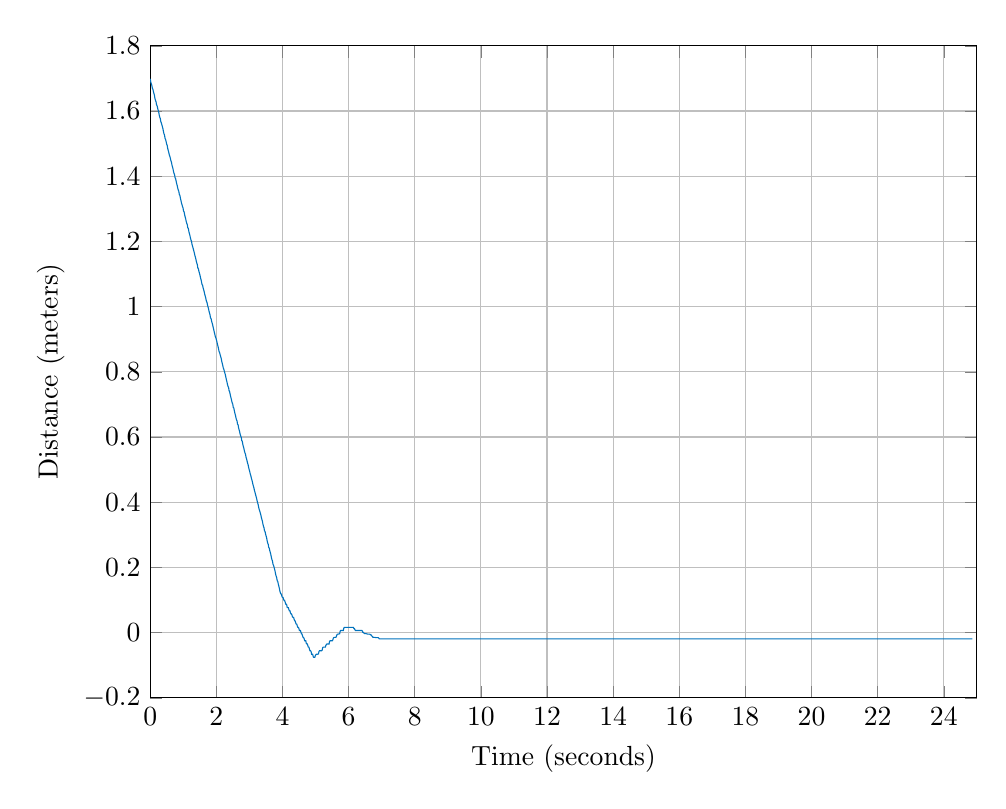
\begin{tikzpicture}

\begin{axis}[%
width=4.133in,
height=3.26in,
at={(0.693in,0.44in)},
scale only axis,
xmin=0,
xmax=25,
xmajorgrids,
xlabel={Time (seconds)},
ymin=-0.2,
ymax=1.8,
ymajorgrids,
ylabel={Distance (meters)},
axis background/.style={fill=white}
]
\addplot [color=mycolor1,solid,forget plot]
  table[row sep=crcr]{%
0	1.69871129724401\\
0.0161597069999985	1.68893572639479\\
0.0320381099999994	1.68304748664486\\
0.0480332269999981	1.67912271456059\\
0.0639209419999979	1.66931011561885\\
0.0799915179999992	1.66734738109778\\
0.095894748999998	1.65949784397757\\
0.112236309	1.65361021900933\\
0.128000544	1.64772313251249\\
0.144037290999997	1.63794410885595\\
0.160031794999998	1.63205633442079\\
0.176005682999998	1.62813189575498\\
0.192028402999997	1.61832008838933\\
0.208044257999998	1.61635749467799\\
0.223975831999999	1.60850861976092\\
0.239845890999999	1.60262157886489\\
0.255932509	1.59673502919364\\
0.272045081	1.58734001353617\\
0.288055432999998	1.58106497639806\\
0.303994013	1.57714087404251\\
0.320085219	1.56732994860591\\
0.336047623	1.56340561944332\\
0.352167114	1.55751933829978\\
0.367957239999998	1.55163277667723\\
0.384000864	1.54574694383911\\
0.400002680999998	1.53673752095665\\
0.416095590999998	1.53007361836111\\
0.432093585999999	1.52614967659862\\
0.448009974999998	1.51633972033348\\
0.464211726	1.51241574277692\\
0.480004193999998	1.5065299349548\\
0.495950020999998	1.49868218733043\\
0.512157272999998	1.49475848376015\\
0.527974259999998	1.48574768432082\\
0.543906164999999	1.4790821002072\\
0.559931816999998	1.47319656333825\\
0.576047603	1.4653494447477\\
0.592099309	1.4614252420419\\
0.607958182999998	1.45554052188685\\
0.624044353999998	1.44769340723938\\
0.640059370999999	1.44377015708712\\
0.655988042999998	1.4347569579997\\
0.674189583999999	1.42809050499233\\
0.689372704999998	1.42220547781748\\
0.704676809999999	1.41435912230833\\
0.720098040999997	1.40847385303638\\
0.736003673999999	1.40455114742055\\
0.751938995999999	1.39474336036922\\
0.768141095999997	1.39278164787541\\
0.783864349999998	1.38415554707216\\
0.799962436000001	1.37709909106128\\
0.816062182	1.37121450744656\\
0.831906223999999	1.36336883703143\\
0.848027445999999	1.35748408737176\\
0.863959540999997	1.35356162772472\\
0.879933877999999	1.34375472787583\\
0.896142252999999	1.34179332640154\\
0.911980344	1.3327763641861\\
0.927973438999999	1.32610752584645\\
0.944083456999999	1.31826243875527\\
0.961772406999998	1.31237855057905\\
0.977025619999997	1.30649432253796\\
0.992100941	1.30257231269253\\
1.008016162	1.29276624303506\\
1.024052284	1.29080502488716\\
1.040043836	1.28178351599921\\
1.056101456	1.27511612308704\\
1.072042082	1.2692326481451\\
1.088003722	1.26138833611554\\
1.104018756	1.25550464929934\\
1.120016068	1.25158296727092\\
1.136028841	1.24177772607526\\
1.152454134	1.23981668476706\\
1.168027	1.2303995072145\\
1.184022474	1.22412476633608\\
1.200019596	1.21824182103829\\
1.215844534	1.21039822757948\\
1.231866587	1.20451505767636\\
1.248032203	1.2005937590141\\
1.263980122	1.19078942043123\\
1.280011167	1.18490673794708\\
1.29606839	1.17940870504848\\
1.311915058	1.17313356596483\\
1.328096262	1.1672510988771\\
1.344009535	1.15940824885514\\
1.360016657	1.15352569176184\\
1.375985619	1.14764371378953\\
1.392028144	1.13980142041503\\
1.40798655	1.13391921114855\\
1.42402477	1.12841776192211\\
1.440059497	1.11822158188759\\
1.45603875	1.1162605804508\\
1.471952503	1.1084184254641\\
1.488035673	1.10253629143816\\
1.503981907	1.09665490151816\\
1.519956103	1.08881312554247\\
1.536030251	1.08293152143553\\
1.552009798	1.07507267952918\\
1.568032618	1.06723098008438\\
1.5838202	1.06527019760318\\
1.599864249	1.05742876912491\\
1.615959169	1.05154727112046\\
1.632048688	1.04566638010345\\
1.648019474	1.03782551190427\\
1.664054938	1.03194436384094\\
1.679953888	1.02604218763219\\
1.698397633	1.01624058473149\\
1.713703745	1.01428004472839\\
1.72889844	1.00643932715905\\
1.744129695	1.00055847314288\\
1.759945545	0.994677953425816\\
1.776049409	0.986837802029016\\
1.792043329	0.980558688723852\\
1.807978683	0.975051181247059\\
1.82404031	0.965250506013386\\
1.839987489	0.96329011844845\\
1.855994895	0.955450129911461\\
1.872343168	0.94956970168786\\
1.889012394	0.943689914530665\\
1.9044551	0.935850489903957\\
1.919998366	0.929570993774472\\
1.936042599	0.922100180707373\\
1.9551955	0.914260636445593\\
1.967938604	0.908380570722335\\
1.983951515	0.904461289654192\\
1.999907206	0.898581464602012\\
2.015889816	0.892702168501254\\
2.031923368	0.884863548697085\\
2.048048731	0.878584115504906\\
2.064144898	0.871109887908198\\
2.079977502	0.863271098039109\\
2.096045085	0.859350967097983\\
2.112068737	0.853472564200506\\
2.128073517	0.847593340588921\\
2.144261578	0.841714550055185\\
2.160036456	0.833876587396984\\
2.176083732	0.826396763295437\\
2.192723347	0.820119933701045\\
2.208038736	0.812281855159503\\
2.223876149	0.808362164955397\\
2.239849326	0.802484373461212\\
2.255899088	0.796605666066156\\
2.272052215	0.790727458630502\\
2.287967036	0.782890319311338\\
2.304064223	0.775407591406852\\
2.320043139	0.769130319900535\\
2.336038054	0.761293068547499\\
2.351829435	0.75541467613456\\
2.369982512	0.751496479134997\\
2.38512788	0.74170016002278\\
2.400280705	0.739740988787028\\
2.415837345	0.731501518293285\\
2.432007665	0.724418512415375\\
2.448062212	0.718141068284811\\
2.463904847	0.710304473858481\\
2.480109883	0.704426707604771\\
2.496265234	0.700508883353315\\
2.512023521	0.690713360854889\\
2.528088527	0.688754202437095\\
2.544039715	0.680515038507873\\
2.559966231	0.673029345138253\\
2.576072755	0.667152253082086\\
2.592026031	0.659316504360529\\
2.608029787	0.653439253292801\\
2.624161381	0.649521810331318\\
2.640087182	0.639727347084461\\
2.656085963	0.637768618929747\\
2.671960964	0.62872082387013\\
2.687938773	0.622040424101864\\
2.704019966	0.616163989895688\\
2.719945606	0.608328904385657\\
2.738228445	0.602452118238467\\
2.753453936	0.598535052312638\\
2.768958834	0.588741386154098\\
2.784172406	0.586782953034807\\
2.799987707	0.577330655479049\\
2.815978062	0.571051900275226\\
2.831936446	0.565175920436754\\
2.848171315	0.557341692739733\\
2.864070536	0.551465599918871\\
2.879906841	0.547548920191658\\
2.898319483	0.537756332694852\\
2.913432974	0.533433205478571\\
2.928504284	0.526343085141848\\
2.944032319	0.520063962159091\\
2.961627301	0.514188695073108\\
2.976743491	0.506355081664197\\
2.991888999	0.500479650243511\\
3.008038559	0.494604892109511\\
3.024039035	0.486771711290253\\
3.040029301	0.482041069001969\\
3.056029827	0.474951959878612\\
3.072002385	0.469076411879514\\
3.087935715	0.46320174307167\\
3.104126096	0.455368866665759\\
3.12008357	0.449493948992479\\
3.13626276	0.443619792502053\\
3.151976129	0.435787349831549\\
3.168037998	0.430648428519785\\
3.183919051	0.423964328230578\\
3.200040116	0.418089576280482\\
3.216189738	0.412215493214756\\
3.231910769	0.404383364085438\\
3.248055819	0.398509125431866\\
3.264056188	0.392635554648707\\
3.280027158	0.384395210111485\\
3.296231439	0.377298609904035\\
3.312036912	0.372977597796839\\
3.328016334	0.367103377074015\\
3.343968255	0.361229909607538\\
3.360014117	0.353398805192615\\
3.376034012	0.347524948726206\\
3.392055329	0.341651996907191\\
3.408026453	0.333001963896481\\
3.424020107	0.326312818280381\\
3.440119185	0.321991261436119\\
3.45601791	0.312202244186959\\
3.471905818	0.310244617298781\\
3.487985074	0.302414352466512\\
3.504023751	0.296540955638987\\
3.520007506	0.290668589105361\\
3.536027933	0.281608342510867\\
3.55201356	0.274920238752738\\
3.568069104	0.271005653666978\\
3.583991387	0.261217606003176\\
3.599856609	0.259260325908042\\
3.615886901	0.251430789588521\\
3.631882137	0.245558077424806\\
3.648018395	0.239275305161136\\
3.664186224	0.230215965222551\\
3.680057807	0.223934969536399\\
3.69610339099999	0.220020579845011\\
3.712014664	0.210234035078069\\
3.727875202	0.206319521438501\\
3.746120862	0.200447621778105\\
3.761399832	0.19457537383804\\
3.777495913	0.187469394394467\\
3.792651319	0.179231291646869\\
3.808047239	0.172950077713062\\
3.824017838	0.169036360464767\\
3.840128517	0.159250183080458\\
3.856000751	0.157293420718972\\
3.872034177	0.149465470882983\\
3.888009325	0.143181163778427\\
3.904088042	0.136485513695991\\
3.919988997	0.127837780808854\\
3.936021406	0.12196625098542\\
3.95416299399999	0.118053047831513\\
3.969390648	0.118053671948953\\
3.984691207	0.110225493363726\\
3.999839993	0.108269543967233\\
4.016042797	0.108270330969134\\
4.03203006	0.102399395843292\\
4.048061705	0.0984862594713412\\
4.06407144	0.0984872886415111\\
4.080018434	0.0941594451900318\\
4.096129343	0.0874625463582588\\
4.112024089	0.0874628361458927\\
4.127970745	0.0850950626059361\\
4.143969595	0.0768571351875145\\
4.160082283	0.0768575072346276\\
4.176027659	0.0768581011423619\\
4.192031024	0.0709877188160699\\
4.207906927	0.0670753752405857\\
4.224030191	0.0670761330116969\\
4.240131932	0.0612060493879958\\
4.256005005	0.0572940154216122\\
4.272005968	0.0572949372945433\\
4.287987546	0.0533815204179826\\
4.304032883	0.0475134286717198\\
4.320066543	0.0470990329475192\\
4.335935542	0.0466838392976991\\
4.351989792	0.0403991501322358\\
4.368078106	0.0364877379760677\\
4.384024383	0.0356612134958443\\
4.400048635	0.0297920471689561\\
4.416002176	0.0258799004666967\\
4.432025753	0.0258806330229335\\
4.448008253	0.0200118494713066\\
4.466390864	0.0160999309655905\\
4.481743225	0.0161008286024771\\
4.496877657	0.0121885054519431\\
4.512207512	0.0063207381724133\\
4.528158156	0.00632180112834302\\
4.544037839	0.00632242136469596\\
4.560025981	0.000454404614969484\\
4.576041295	-0.00387363753753234\\
4.592056829	-0.00470731206715502\\
4.608019278	-0.0105756275646269\\
4.62403573	-0.0149013097434754\\
4.640037472	-0.0153156631968081\\
4.655998012	-0.0192277355455215\\
4.672033909	-0.0250945070702824\\
4.687984735	-0.0250939779766068\\
4.704018982	-0.0250934595164349\\
4.720118501	-0.0329173827984737\\
4.736174136	-0.0348721248013601\\
4.752146888	-0.0348709099965969\\
4.768025783	-0.0407386728914312\\
4.784058266	-0.0446489610539258\\
4.800029234	-0.044647578759978\\
4.815947588	-0.0509339354580634\\
4.832000617	-0.0556813610305149\\
4.848042019	-0.0556809219308558\\
4.864082611	-0.0576362044890137\\
4.879951488	-0.0662910094797866\\
4.89594289	-0.0662904863547429\\
4.912064377	-0.0662894509891434\\
4.9304653	-0.0741117093876493\\
4.94577737	-0.0760665953911499\\
4.961679111	-0.0760653917960896\\
4.977120934	-0.0760643414184479\\
4.993380468	-0.0701963671843349\\
5.007918377	-0.0682398683273959\\
5.023956583	-0.0662835217940423\\
5.040158076	-0.0662835217940423\\
5.055902977	-0.0662824211216588\\
5.072024647	-0.0658643349305423\\
5.088030083	-0.0654448321368184\\
5.10386294	-0.0576215921086409\\
5.120073524	-0.0556658255702775\\
5.136060234	-0.055664318797668\\
5.152007599	-0.0556638147487121\\
5.168071171	-0.0556628174756462\\
5.183948769	-0.0556612890786246\\
5.200052768	-0.0537051345904236\\
5.216022674	-0.0465737605981631\\
5.232006657	-0.0446172304217491\\
5.248422187	-0.0446164371258764\\
5.263848381	-0.0446148612865487\\
5.279826202	-0.044613435982205\\
5.296176005	-0.0446126319339388\\
5.311981721	-0.0387450693181646\\
5.327945374	-0.0367888634441205\\
5.344000982	-0.0348331431779674\\
5.359946961	-0.0348324128066471\\
5.376003225	-0.0348310055285577\\
5.392103125	-0.0348303500075755\\
5.4080127	-0.0348288571865003\\
5.424028947	-0.0270078227380737\\
5.440033359	-0.0250517945274167\\
5.456060079	-0.0250504279724031\\
5.47202798	-0.025049739378282\\
5.487982025	-0.0250485216894465\\
5.504321258	-0.0250478224621185\\
5.520074267	-0.0230912347651395\\
5.536756396	-0.0172256489887266\\
5.552058505	-0.0152703289659444\\
5.568074951	-0.0148481242482632\\
5.584150324	-0.0144250438543301\\
5.600060666	-0.0144243973948623\\
5.616020499	-0.0144231150495533\\
5.632025239	-0.0105112662723323\\
5.648037045	-0.00660175890715542\\
5.664116752	-0.00464606729543604\\
5.679942383	-0.00464437671218132\\
5.698385246	-0.00464437671218132\\
5.713696811	-0.00336876985330625\\
5.728932413	-0.00336783530132267\\
5.744098644	0.0044522415300019\\
5.760014211	0.0064083608881389\\
5.775945737	0.00640923172839569\\
5.79213369	0.00641081678433286\\
5.808040699	0.00641169806611774\\
5.823987022	0.00641345018815964\\
5.840063859	0.00641505612753535\\
5.85608706	0.0142336466099027\\
5.872151891	0.0161895107638446\\
5.88801638	0.0161909898158903\\
5.904064434	0.0161918175892559\\
5.919998809	0.0161934627540379\\
5.93607576	0.0161949625703395\\
5.954263675	0.0161958007256291\\
5.968022303	0.0161974666542841\\
5.983883145	0.0161989872347965\\
6.000049104	0.0161998357719848\\
6.015938219	0.0162006739272744\\
6.032082775	0.0162030638091391\\
6.04805246	0.0162030638091391\\
6.064082037	0.0162047712653877\\
6.080065318	0.0162056301844482\\
6.096283305	0.016207192293243\\
6.112111165	0.0162089205132103\\
6.12803681	0.0162097898141171\\
6.144032264	0.0162113726869815\\
6.15999543899999	0.0123042193904623\\
6.176025307	0.0123060430035689\\
6.192050662	0.00839983725200977\\
6.207921611	0.00644715815732333\\
6.22418061	0.00644907734205402\\
6.239899469	0.00645085034712545\\
6.255993164	0.00645182560141855\\
6.271981044	0.00645376566872891\\
6.288022904	0.0064555595567759\\
6.304075306	0.00645654525231443\\
6.320040812	0.00645850620214539\\
6.336001828	0.00646032097311311\\
6.35187561	0.00646131710986664\\
6.368084163	0.00646230280540494\\
6.383953458	0.00646329894215891\\
6.400024741	0.00646513459599229\\
6.416083481	0.00451326951456554\\
6.432049987	0.000606989229278154\\
6.448068159	0.000608994846316602\\
6.464017704	-0.00134318265871802\\
6.480020071	-0.00329427859929332\\
6.496229008	-0.00329225198046768\\
6.511858828	-0.00329114941473319\\
6.530239581	-0.00328895478388502\\
6.5453811	-0.00371740052756842\\
6.560536606	-0.00414678081236741\\
6.575981488	-0.00457574031183228\\
6.592027873	-0.00457367168961809\\
6.608653865	-0.00457288898670516\\
6.624052054	-0.00457133409455657\\
6.640030645	-0.00456924447074214\\
6.656037202	-0.00652194560537556\\
6.671994857	-0.00652116290246241\\
6.687993142	-0.00847393884510206\\
6.704031864	-0.0104246475733203\\
6.720040167	-0.0123757937441658\\
6.735860388	-0.0143278084155758\\
6.752142985	-0.0143255269942206\\
6.767895372	-0.0147532289280985\\
6.783825069	-0.0147523392813249\\
6.799921703	-0.0147503776559519\\
6.815882875	-0.0151789480904481\\
6.832018811	-0.0151771582238365\\
6.848020074	-0.0151755163814231\\
6.864051549	-0.0151746055885482\\
6.880044717	-0.0151727945758353\\
6.896191653	-0.0151711315869532\\
6.912056843	-0.0171233296396782\\
6.92827234	-0.0190746920050473\\
6.944046239	-0.0190746920050473\\
6.961524159	-0.0190746920050473\\
6.977450972	-0.0190746920050473\\
6.992599246	-0.0190746920050473\\
7.008127417	-0.0190746920050473\\
7.023842395	-0.0190746920050473\\
7.040040934	-0.0190746920050473\\
7.056096008	-0.0190746920050473\\
7.072035099	-0.0190746920050473\\
7.088049521	-0.0190746920050473\\
7.104026435	-0.0190746920050473\\
7.120011623	-0.0190746920050473\\
7.136038122	-0.0190746920050473\\
7.152012828	-0.0190746920050473\\
7.167907396	-0.0190746920050473\\
7.184216646	-0.0190746920050473\\
7.200091968	-0.0190746920050473\\
7.215989592	-0.0190746920050473\\
7.231833071	-0.0190746920050473\\
7.248330282	-0.0190746920050473\\
7.26403765	-0.0190746920050473\\
7.279981706	-0.0190746920050473\\
7.296229812	-0.0190746920050473\\
7.312106607	-0.0190746920050473\\
7.328115852	-0.0190746920050473\\
7.347357186	-0.0190746920050473\\
7.360618501	-0.0190746920050473\\
7.375853683	-0.0190746920050473\\
7.392082657	-0.0190746920050473\\
7.408037023	-0.0190746920050473\\
7.424167001	-0.0190746920050473\\
7.440051263	-0.0190746920050473\\
7.455951863	-0.0190746920050473\\
7.471980511	-0.0190746920050473\\
7.488062711	-0.0190746920050473\\
7.50406574399999	-0.0190746920050473\\
7.520029658	-0.0190746920050473\\
7.536123601	-0.0190746920050473\\
7.551947701	-0.0190746920050473\\
7.568152163	-0.0190746920050473\\
7.584046088	-0.0190746920050473\\
7.59997950499999	-0.0190746920050473\\
7.615931435	-0.0190746920050473\\
7.63193073299999	-0.0190746920050473\\
7.647994752	-0.0190746920050473\\
7.664175922	-0.0190746920050473\\
7.679965259	-0.0190746920050473\\
7.695999804	-0.0190746920050473\\
7.712042392	-0.0190746920050473\\
7.728070754	-0.0190746920050473\\
7.74400096	-0.0190746920050473\\
7.760090146	-0.0190746920050473\\
7.775972463	-0.0190746920050473\\
7.79210594	-0.0190746920050473\\
7.807910945	-0.0190746920050473\\
7.826481575	-0.0190746920050473\\
7.840035591	-0.0190746920050473\\
7.855958237	-0.0190746920050473\\
7.872038788	-0.0190746920050473\\
7.887981322	-0.0190746920050473\\
7.90405819	-0.0190746920050473\\
7.920025129	-0.0190746920050473\\
7.936070311	-0.0190746920050473\\
7.95442091	-0.0190746920050473\\
7.970032808	-0.0190746920050473\\
7.985465228	-0.0190746920050473\\
8.000631693	-0.0190746920050473\\
8.015877657	-0.0190746920050473\\
8.031841158	-0.0190746920050473\\
8.048041935	-0.0190746920050473\\
8.064091872	-0.0190746920050473\\
8.080200063	-0.0190746920050473\\
8.096275027	-0.0190746920050473\\
8.112130566	-0.0190746920050473\\
8.128056864	-0.0190746920050473\\
8.143986503	-0.0190746920050473\\
8.16003903099999	-0.0190746920050473\\
8.176019812	-0.0190746920050473\\
8.192062197	-0.0190746920050473\\
8.207986459	-0.0190746920050473\\
8.223936542	-0.0190746920050473\\
8.240084434	-0.0190746920050473\\
8.25601462	-0.0190746920050473\\
8.27198565599999	-0.0190746920050473\\
8.288014618	-0.0190746920050473\\
8.304042044	-0.0190746920050473\\
8.320048804	-0.0190746920050473\\
8.336020914	-0.0190746920050473\\
8.352109304	-0.0190746920050473\\
8.368036166	-0.0190746920050473\\
8.384032565	-0.0190746920050473\\
8.400153247	-0.0190746920050473\\
8.416017998	-0.0190746920050473\\
8.432060103	-0.0190746920050473\\
8.448029026	-0.0190746920050473\\
8.464155182	-0.0190746920050473\\
8.479910554	-0.0190746920050473\\
8.496110741	-0.0190746920050473\\
8.512041377	-0.0190746920050473\\
8.528053603	-0.0190746920050473\\
8.5440378	-0.0190746920050473\\
8.560008308	-0.0190746920050473\\
8.576030592	-0.0190746920050473\\
8.592044783	-0.0190746920050473\\
8.608031017	-0.0190746920050473\\
8.62401557499999	-0.0190746920050473\\
8.640046203	-0.0190746920050473\\
8.656053173	-0.0190746920050473\\
8.672049955	-0.0190746920050473\\
8.688048636	-0.0190746920050473\\
8.704018567	-0.0190746920050473\\
8.720117199	-0.0190746920050473\\
8.735884545	-0.0190746920050473\\
8.752065129	-0.0190746920050473\\
8.768022497	-0.0190746920050473\\
8.783983003	-0.0190746920050473\\
8.800052132	-0.0190746920050473\\
8.81598551999999	-0.0190746920050473\\
8.832077187	-0.0190746920050473\\
8.848160304	-0.0190746920050473\\
8.864148186	-0.0190746920050473\\
8.880060631	-0.0190746920050473\\
8.896150063	-0.0190746920050473\\
8.91204172199999	-0.0190746920050473\\
8.928087221	-0.0190746920050473\\
8.943992198	-0.0190746920050473\\
8.962038489	-0.0190746920050473\\
8.97723275499999	-0.0190746920050473\\
8.992413163	-0.0190746920050473\\
9.008046767	-0.0190746920050473\\
9.024117446	-0.0190746920050473\\
9.040125834	-0.0190746920050473\\
9.05604500499999	-0.0190746920050473\\
9.072428207	-0.0190746920050473\\
9.088008385	-0.0190746920050473\\
9.104071111	-0.0190746920050473\\
9.119975429	-0.0190746920050473\\
9.135911819	-0.0190746920050473\\
9.152010125	-0.0190746920050473\\
9.168027158	-0.0190746920050473\\
9.183971459	-0.0190746920050473\\
9.200329666	-0.0190746920050473\\
9.216105473	-0.0190746920050473\\
9.231951862	-0.0190746920050473\\
9.247956231	-0.0190746920050473\\
9.263936089	-0.0190746920050473\\
9.27997825499999	-0.0190746920050473\\
9.296043407	-0.0190746920050473\\
9.31200781	-0.0190746920050473\\
9.328068476	-0.0190746920050473\\
9.343996109	-0.0190746920050473\\
9.360029443	-0.0190746920050473\\
9.376059964	-0.0190746920050473\\
9.392060099	-0.0190746920050473\\
9.408022713	-0.0190746920050473\\
9.424026481	-0.0190746920050473\\
9.439842754	-0.0190746920050473\\
9.45612246099999	-0.0190746920050473\\
9.47194129	-0.0190746920050473\\
9.487846234	-0.0190746920050473\\
9.503996775	-0.0190746920050473\\
9.520063444	-0.0190746920050473\\
9.53605973	-0.0190746920050473\\
9.551842657	-0.0190746920050473\\
9.567985474	-0.0190746920050473\\
9.583973095	-0.0190746920050473\\
9.600094845	-0.0190746920050473\\
9.615999506	-0.0190746920050473\\
9.63206045	-0.0190746920050473\\
9.647986517	-0.0190746920050473\\
9.66403696	-0.0190746920050473\\
9.6800219	-0.0190746920050473\\
9.69633846499999	-0.0190746920050473\\
9.71200180299999	-0.0190746920050473\\
9.727943566	-0.0190746920050473\\
9.743880255	-0.0190746920050473\\
9.760009592	-0.0190746920050473\\
9.77591782	-0.0190746920050473\\
9.792128023	-0.0190746920050473\\
9.807998384	-0.0190746920050473\\
9.824041778	-0.0190746920050473\\
9.839929408	-0.0190746920050473\\
9.856133159	-0.0190746920050473\\
9.87203671	-0.0190746920050473\\
9.887991558	-0.0190746920050473\\
9.904069088	-0.0190746920050473\\
9.91998593899999	-0.0190746920050473\\
9.936009968	-0.0190746920050473\\
9.954419339	-0.0190746920050473\\
9.969493511	-0.0190746920050473\\
9.984564415	-0.0190746920050473\\
9.999949428	-0.0190746920050473\\
10.01603085	-0.0190746920050473\\
10.031982539	-0.0190746920050473\\
10.047971055	-0.0190746920050473\\
10.064137549	-0.0190746920050473\\
10.080024832	-0.0190746920050473\\
10.096311882	-0.0190746920050473\\
10.111981522	-0.0190746920050473\\
10.128014125	-0.0190746920050473\\
10.143918003	-0.0190746920050473\\
10.160075898	-0.0190746920050473\\
10.176041825	-0.0190746920050473\\
10.191946311	-0.0190746920050473\\
10.207993503	-0.0190746920050473\\
10.223840547	-0.0190746920050473\\
10.242181889	-0.0190746920050473\\
10.257547214	-0.0190746920050473\\
10.272842035	-0.0190746920050473\\
10.288258415	-0.0190746920050473\\
10.30402324	-0.0190746920050473\\
10.319987257	-0.0190746920050473\\
10.336007504	-0.0190746920050473\\
10.351845281	-0.0190746920050473\\
10.367901405	-0.0190746920050473\\
10.383952171	-0.0190746920050473\\
10.400084774	-0.0190746920050473\\
10.416048786	-0.0190746920050473\\
10.432052679	-0.0190746920050473\\
10.447944806	-0.0190746920050473\\
10.464018899	-0.0190746920050473\\
10.479930656	-0.0190746920050473\\
10.496009384	-0.0190746920050473\\
10.512003509	-0.0190746920050473\\
10.528001341	-0.0190746920050473\\
10.543906675	-0.0190746920050473\\
10.560054811	-0.0190746920050473\\
10.575963898	-0.0190746920050473\\
10.592071361	-0.0190746920050473\\
10.608016686	-0.0190746920050473\\
10.624253612	-0.0190746920050473\\
10.639974423	-0.0190746920050473\\
10.656005623	-0.0190746920050473\\
10.6720202	-0.0190746920050473\\
10.688051613	-0.0190746920050473\\
10.704094484	-0.0190746920050473\\
10.719905633	-0.0190746920050473\\
10.736099586	-0.0190746920050473\\
10.752060592	-0.0190746920050473\\
10.767958262	-0.0190746920050473\\
10.78385751	-0.0190746920050473\\
10.800008416	-0.0190746920050473\\
10.815938755	-0.0190746920050473\\
10.832015205	-0.0190746920050473\\
10.84798706	-0.0190746920050473\\
10.863915459	-0.0190746920050473\\
10.879975807	-0.0190746920050473\\
10.896156141	-0.0190746920050473\\
10.912156856	-0.0190746920050473\\
10.928125038	-0.0190746920050473\\
10.94389824	-0.0190746920050473\\
10.961753412	-0.0190746920050473\\
10.976892011	-0.0190746920050473\\
10.991989265	-0.0190746920050473\\
11.007936167	-0.0190746920050473\\
11.023980819	-0.0190746920050473\\
11.039995061	-0.0190746920050473\\
11.055939814	-0.0190746920050473\\
11.072026706	-0.0190746920050473\\
11.087993069	-0.0190746920050473\\
11.104061448	-0.0190746920050473\\
11.119990536	-0.0190746920050473\\
11.13604776	-0.0190746920050473\\
11.151991937	-0.0190746920050473\\
11.167951617	-0.0190746920050473\\
11.184098376	-0.0190746920050473\\
11.200034054	-0.0190746920050473\\
11.216048521	-0.0190746920050473\\
11.232185	-0.0190746920050473\\
11.247942829	-0.0190746920050473\\
11.264146716	-0.0190746920050473\\
11.279973192	-0.0190746920050473\\
11.296176855	-0.0190746920050473\\
11.312011646	-0.0190746920050473\\
11.32802642	-0.0190746920050473\\
11.344102481	-0.0190746920050473\\
11.360021482	-0.0190746920050473\\
11.375974636	-0.0190746920050473\\
11.392056679	-0.0190746920050473\\
11.408017455	-0.0190746920050473\\
11.424039889	-0.0190746920050473\\
11.440068771	-0.0190746920050473\\
11.455963834	-0.0190746920050473\\
11.472028245	-0.0190746920050473\\
11.487850341	-0.0190746920050473\\
11.503963567	-0.0190746920050473\\
11.519898403	-0.0190746920050473\\
11.536050687	-0.0190746920050473\\
11.55205493	-0.0190746920050473\\
11.568074338	-0.0190746920050473\\
11.583873613	-0.0190746920050473\\
11.600053498	-0.0190746920050473\\
11.615978068	-0.0190746920050473\\
11.632026927	-0.0190746920050473\\
11.647987738	-0.0190746920050473\\
11.664023823	-0.0190746920050473\\
11.679976365	-0.0190746920050473\\
11.696077372	-0.0190746920050473\\
11.71197076	-0.0190746920050473\\
11.727841005	-0.0190746920050473\\
11.744121961	-0.0190746920050473\\
11.760058751	-0.0190746920050473\\
11.775981456	-0.0190746920050473\\
11.792139803	-0.0190746920050473\\
11.808040402	-0.0190746920050473\\
11.824030439	-0.0190746920050473\\
11.839930198	-0.0190746920050473\\
11.856071871	-0.0190746920050473\\
11.872051192	-0.0190746920050473\\
11.887960344	-0.0190746920050473\\
11.904064275	-0.0190746920050473\\
11.920007937	-0.0190746920050473\\
11.936042439	-0.0190746920050473\\
11.954345124	-0.0190746920050473\\
11.969600887	-0.0190746920050473\\
11.984774743	-0.0190746920050473\\
12.000021787	-0.0190746920050473\\
12.015990606	-0.0190746920050473\\
12.032030576	-0.0190746920050473\\
12.048008515	-0.0190746920050473\\
12.064101971	-0.0190746920050473\\
12.079999859	-0.0190746920050473\\
12.096173406	-0.0190746920050473\\
12.111978598	-0.0190746920050473\\
12.128102533	-0.0190746920050473\\
12.143986169	-0.0190746920050473\\
12.159931471	-0.0190746920050473\\
12.175995508	-0.0190746920050473\\
12.192126894	-0.0190746920050473\\
12.207915106	-0.0190746920050473\\
12.223849699	-0.0190746920050473\\
12.240104586	-0.0190746920050473\\
12.255989618	-0.0190746920050473\\
12.272108488	-0.0190746920050473\\
12.288026742	-0.0190746920050473\\
12.304032474	-0.0190746920050473\\
12.319919155	-0.0190746920050473\\
12.336026423	-0.0190746920050473\\
12.351984568	-0.0190746920050473\\
12.36799499	-0.0190746920050473\\
12.383991041	-0.0190746920050473\\
12.40011831	-0.0190746920050473\\
12.415925558	-0.0190746920050473\\
12.432058415	-0.0190746920050473\\
12.44804794	-0.0190746920050473\\
12.464110415	-0.0190746920050473\\
12.479914115	-0.0190746920050473\\
12.495969561	-0.0190746920050473\\
12.512145343	-0.0190746920050473\\
12.528196013	-0.0190746920050473\\
12.543936511	-0.0190746920050473\\
12.559966416	-0.0190746920050473\\
12.575993634	-0.0190746920050473\\
12.592045531	-0.0190746920050473\\
12.607943409	-0.0190746920050473\\
12.624102934	-0.0190746920050473\\
12.640012173	-0.0190746920050473\\
12.65615738	-0.0190746920050473\\
12.672005105	-0.0190746920050473\\
12.687947837	-0.0190746920050473\\
12.703857148	-0.0190746920050473\\
12.719957478	-0.0190746920050473\\
12.735929695	-0.0190746920050473\\
12.751939591	-0.0190746920050473\\
12.76804339	-0.0190746920050473\\
12.783981093	-0.0190746920050473\\
12.800015786	-0.0190746920050473\\
12.815985707	-0.0190746920050473\\
12.832077238	-0.0190746920050473\\
12.847975226	-0.0190746920050473\\
12.863951035	-0.0190746920050473\\
12.879817968	-0.0190746920050473\\
12.898329922	-0.0190746920050473\\
12.913635623	-0.0190746920050473\\
12.928822896	-0.0190746920050473\\
12.944141417	-0.0190746920050473\\
12.961861101	-0.0190746920050473\\
12.977067905	-0.0190746920050473\\
12.992354105	-0.0190746920050473\\
13.007968762	-0.0190746920050473\\
13.024084042	-0.0190746920050473\\
13.041294187	-0.0190746920050473\\
13.056377386	-0.0190746920050473\\
13.071859735	-0.0190746920050473\\
13.088020699	-0.0190746920050473\\
13.104060779	-0.0190746920050473\\
13.120021364	-0.0190746920050473\\
13.136209198	-0.0190746920050473\\
13.15198511	-0.0190746920050473\\
13.167973415	-0.0190746920050473\\
13.183933769	-0.0190746920050473\\
13.199982266	-0.0190746920050473\\
13.216107117	-0.0190746920050473\\
13.231896675	-0.0190746920050473\\
13.247975103	-0.0190746920050473\\
13.265740064	-0.0190746920050473\\
13.280772699	-0.0190746920050473\\
13.296028956	-0.0190746920050473\\
13.311972453	-0.0190746920050473\\
13.32817736	-0.0190746920050473\\
13.344024287	-0.0190746920050473\\
13.360055672	-0.0190746920050473\\
13.375948308	-0.0190746920050473\\
13.392040151	-0.0190746920050473\\
13.407889418	-0.0190746920050473\\
13.424004142	-0.0190746920050473\\
13.440038052	-0.0190746920050473\\
13.4560137	-0.0190746920050473\\
13.472000736	-0.0190746920050473\\
13.490213617	-0.0190746920050473\\
13.505429094	-0.0190746920050473\\
13.52066168	-0.0190746920050473\\
13.536031341	-0.0190746920050473\\
13.552165255	-0.0190746920050473\\
13.568039037	-0.0190746920050473\\
13.583982463	-0.0190746920050473\\
13.600090446	-0.0190746920050473\\
13.616007713	-0.0190746920050473\\
13.632086251	-0.0190746920050473\\
13.648004273	-0.0190746920050473\\
13.663916969	-0.0190746920050473\\
13.679885169	-0.0190746920050473\\
13.69607269	-0.0190746920050473\\
13.711928864	-0.0190746920050473\\
13.727840392	-0.0190746920050473\\
13.746186255	-0.0190746920050473\\
13.761514983	-0.0190746920050473\\
13.776717546	-0.0190746920050473\\
13.792096959	-0.0190746920050473\\
13.808066698	-0.0190746920050473\\
13.824055471	-0.0190746920050473\\
13.840026692	-0.0190746920050473\\
13.85609019	-0.0190746920050473\\
13.872063824	-0.0190746920050473\\
13.88799977	-0.0190746920050473\\
13.90403201	-0.0190746920050473\\
13.919998037	-0.0190746920050473\\
13.935995265	-0.0190746920050473\\
13.95437071	-0.0190746920050473\\
13.969473101	-0.0190746920050473\\
13.984630877	-0.0190746920050473\\
14.000035212	-0.0190746920050473\\
14.016035313	-0.0190746920050473\\
14.031898991	-0.0190746920050473\\
14.047852831	-0.0190746920050473\\
14.064161409	-0.0190746920050473\\
14.079916593	-0.0190746920050473\\
14.096102855	-0.0190746920050473\\
14.111976958	-0.0190746920050473\\
14.12797426	-0.0190746920050473\\
14.144012668	-0.0190746920050473\\
14.160044558	-0.0190746920050473\\
14.175961709	-0.0190746920050473\\
14.192042305	-0.0190746920050473\\
14.208049652	-0.0190746920050473\\
14.224001116	-0.0190746920050473\\
14.240155139	-0.0190746920050473\\
14.256090979	-0.0190746920050473\\
14.272063903	-0.0190746920050473\\
14.28797831	-0.0190746920050473\\
14.303983426	-0.0190746920050473\\
14.320013633	-0.0190746920050473\\
14.336042573	-0.0190746920050473\\
14.351997199	-0.0190746920050473\\
14.36802878	-0.0190746920050473\\
14.383966503	-0.0190746920050473\\
14.400057874	-0.0190746920050473\\
14.415985273	-0.0190746920050473\\
14.432045383	-0.0190746920050473\\
14.448058382	-0.0190746920050473\\
14.46406445	-0.0190746920050473\\
14.479910137	-0.0190746920050473\\
14.49607347	-0.0190746920050473\\
14.512028174	-0.0190746920050473\\
14.527908512	-0.0190746920050473\\
14.543920158	-0.0190746920050473\\
14.560094903	-0.0190746920050473\\
14.575994334	-0.0190746920050473\\
14.592083014	-0.0190746920050473\\
14.608016698	-0.0190746920050473\\
14.623979878	-0.0190746920050473\\
14.640039582	-0.0190746920050473\\
14.658631804	-0.0190746920050473\\
14.673926435	-0.0190746920050473\\
14.689106326	-0.0190746920050473\\
14.704237437	-0.0190746920050473\\
14.720017432	-0.0190746920050473\\
14.736000604	-0.0190746920050473\\
14.751897312	-0.0190746920050473\\
14.76799095	-0.0190746920050473\\
14.783951428	-0.0190746920050473\\
14.799989254	-0.0190746920050473\\
14.816017647	-0.0190746920050473\\
14.83207217	-0.0190746920050473\\
14.847917306	-0.0190746920050473\\
14.864260418	-0.0190746920050473\\
14.880000474	-0.0190746920050473\\
14.896367052	-0.0190746920050473\\
14.911982171	-0.0190746920050473\\
14.928100222	-0.0190746920050473\\
14.943937995	-0.0190746920050473\\
14.961505084	-0.0190746920050473\\
14.976719449	-0.0190746920050473\\
14.992708124	-0.0190746920050473\\
15.008074242	-0.0190746920050473\\
15.024059109	-0.0190746920050473\\
15.040035048	-0.0190746920050473\\
15.055998653	-0.0190746920050473\\
15.072032675	-0.0190746920050473\\
15.088002988	-0.0190746920050473\\
15.104054268	-0.0190746920050473\\
15.12001629	-0.0190746920050473\\
15.136030935	-0.0190746920050473\\
15.151992881	-0.0190746920050473\\
15.16803866	-0.0190746920050473\\
15.183995224	-0.0190746920050473\\
15.200043959	-0.0190746920050473\\
15.216020123	-0.0190746920050473\\
15.232088154	-0.0190746920050473\\
15.247962883	-0.0190746920050473\\
15.264254574	-0.0190746920050473\\
15.279998857	-0.0190746920050473\\
15.296281451	-0.0190746920050473\\
15.312007224	-0.0190746920050473\\
15.328021525	-0.0190746920050473\\
15.343924693	-0.0190746920050473\\
15.360020235	-0.0190746920050473\\
15.375979707	-0.0190746920050473\\
15.392074807	-0.0190746920050473\\
15.4080369	-0.0190746920050473\\
15.423993571	-0.0190746920050473\\
15.440044119	-0.0190746920050473\\
15.456149216	-0.0190746920050473\\
15.471981967	-0.0190746920050473\\
15.487863715	-0.0190746920050473\\
15.503998821	-0.0190746920050473\\
15.519946955	-0.0190746920050473\\
15.535932565	-0.0190746920050473\\
15.552059282	-0.0190746920050473\\
15.567950071	-0.0190746920050473\\
15.583928838	-0.0190746920050473\\
15.600016627	-0.0190746920050473\\
15.615932929	-0.0190746920050473\\
15.632057563	-0.0190746920050473\\
15.647974133	-0.0190746920050473\\
15.664152802	-0.0190746920050473\\
15.679981683	-0.0190746920050473\\
15.696198852	-0.0190746920050473\\
15.712040264	-0.0190746920050473\\
15.727842035	-0.0190746920050473\\
15.744097697	-0.0190746920050473\\
15.759945528	-0.0190746920050473\\
15.775844782	-0.0190746920050473\\
15.791876812	-0.0190746920050473\\
15.807852088	-0.0190746920050473\\
15.823862428	-0.0190746920050473\\
15.840023283	-0.0190746920050473\\
15.855884566	-0.0190746920050473\\
15.871958613	-0.0190746920050473\\
15.88802791	-0.0190746920050473\\
15.90401053	-0.0190746920050473\\
15.920018427	-0.0190746920050473\\
15.936069236	-0.0190746920050473\\
15.954402605	-0.0190746920050473\\
15.969881294	-0.0190746920050473\\
15.984989983	-0.0190746920050473\\
16.00027288	-0.0190746920050473\\
16.01600951	-0.0190746920050473\\
16.031859208	-0.0190746920050473\\
16.04780463	-0.0190746920050473\\
16.064065329	-0.0190746920050473\\
16.080016262	-0.0190746920050473\\
16.096154164	-0.0190746920050473\\
16.112023546	-0.0190746920050473\\
16.128038214	-0.0190746920050473\\
16.144233139	-0.0190746920050473\\
16.160047443	-0.0190746920050473\\
16.176083208	-0.0190746920050473\\
16.191986453	-0.0190746920050473\\
16.208033744	-0.0190746920050473\\
16.223970191	-0.0190746920050473\\
16.2398523	-0.0190746920050473\\
16.255910614	-0.0190746920050473\\
16.271863341	-0.0190746920050473\\
16.287877425	-0.0190746920050473\\
16.304023761	-0.0190746920050473\\
16.320012218	-0.0190746920050473\\
16.336074036	-0.0190746920050473\\
16.352134027	-0.0190746920050473\\
16.368204205	-0.0190746920050473\\
16.383995768	-0.0190746920050473\\
16.400038268	-0.0190746920050473\\
16.416009	-0.0190746920050473\\
16.431842075	-0.0190746920050473\\
16.448002864	-0.0190746920050473\\
16.464033426	-0.0190746920050473\\
16.480022769	-0.0190746920050473\\
16.496115231	-0.0190746920050473\\
16.512289109	-0.0190746920050473\\
16.528011935	-0.0190746920050473\\
16.543892275	-0.0190746920050473\\
16.56212276	-0.0190746920050473\\
16.57722955	-0.0190746920050473\\
16.592295954	-0.0190746920050473\\
16.607984222	-0.0190746920050473\\
16.62410717	-0.0190746920050473\\
16.639881247	-0.0190746920050473\\
16.658282741	-0.0190746920050473\\
16.673478132	-0.0190746920050473\\
16.688653213	-0.0190746920050473\\
16.704194162	-0.0190746920050473\\
16.720033512	-0.0190746920050473\\
16.736019635	-0.0190746920050473\\
16.752009501	-0.0190746920050473\\
16.767990572	-0.0190746920050473\\
16.784105401	-0.0190746920050473\\
16.800015231	-0.0190746920050473\\
16.816002061	-0.0190746920050473\\
16.832008619	-0.0190746920050473\\
16.847897314	-0.0190746920050473\\
16.863925596	-0.0190746920050473\\
16.880137952	-0.0190746920050473\\
16.895960994	-0.0190746920050473\\
16.914281783	-0.0190746920050473\\
16.929934661	-0.0190746920050473\\
16.945342984	-0.0190746920050473\\
16.960263709	-0.0190746920050473\\
16.975831538	-0.0190746920050473\\
16.99192098	-0.0190746920050473\\
17.007997753	-0.0190746920050473\\
17.024033474	-0.0190746920050473\\
17.039957638	-0.0190746920050473\\
17.056297991	-0.0190746920050473\\
17.072005116	-0.0190746920050473\\
17.088032337	-0.0190746920050473\\
17.103927044	-0.0190746920050473\\
17.11988812	-0.0190746920050473\\
17.136010334	-0.0190746920050473\\
17.152036342	-0.0190746920050473\\
17.168014692	-0.0190746920050473\\
17.184013078	-0.0190746920050473\\
17.199981288	-0.0190746920050473\\
17.215890801	-0.0190746920050473\\
17.231891825	-0.0190746920050473\\
17.248071937	-0.0190746920050473\\
17.264020134	-0.0190746920050473\\
17.280137368	-0.0190746920050473\\
17.295996117	-0.0190746920050473\\
17.312017424	-0.0190746920050473\\
17.328017744	-0.0190746920050473\\
17.344110368	-0.0190746920050473\\
17.360058365	-0.0190746920050473\\
17.376052275	-0.0190746920050473\\
17.392011561	-0.0190746920050473\\
17.408133216	-0.0190746920050473\\
17.424149582	-0.0190746920050473\\
17.440131154	-0.0190746920050473\\
17.456107625	-0.0190746920050473\\
17.472061494	-0.0190746920050473\\
17.488024953	-0.0190746920050473\\
17.504025396	-0.0190746920050473\\
17.519881624	-0.0190746920050473\\
17.535953396	-0.0190746920050473\\
17.552073427	-0.0190746920050473\\
17.568327787	-0.0190746920050473\\
17.584063126	-0.0190746920050473\\
17.600006793	-0.0190746920050473\\
17.616020482	-0.0190746920050473\\
17.63202191	-0.0190746920050473\\
17.648035049	-0.0190746920050473\\
17.664060666	-0.0190746920050473\\
17.680126274	-0.0190746920050473\\
17.696125887	-0.0190746920050473\\
17.712318614	-0.0190746920050473\\
17.727854137	-0.0190746920050473\\
17.744073049	-0.0190746920050473\\
17.759969957	-0.0190746920050473\\
17.775929065	-0.0190746920050473\\
17.792023494	-0.0190746920050473\\
17.808058412	-0.0190746920050473\\
17.823998105	-0.0190746920050473\\
17.840019477	-0.0190746920050473\\
17.855978844	-0.0190746920050473\\
17.872005428	-0.0190746920050473\\
17.888040291	-0.0190746920050473\\
17.903961697	-0.0190746920050473\\
17.920024659	-0.0190746920050473\\
17.935977917	-0.0190746920050473\\
17.954456165	-0.0190746920050473\\
17.969672849	-0.0190746920050473\\
17.984994447	-0.0190746920050473\\
18.000271955	-0.0190746920050473\\
18.01588217	-0.0190746920050473\\
18.03252904	-0.0190746920050473\\
18.047841275	-0.0190746920050473\\
18.06608627	-0.0190746920050473\\
18.081291205	-0.0190746920050473\\
18.096521953	-0.0190746920050473\\
18.112388562	-0.0190746920050473\\
18.128018843	-0.0190746920050473\\
18.144415454	-0.0190746920050473\\
18.160026689	-0.0190746920050473\\
18.176049735	-0.0190746920050473\\
18.192070411	-0.0190746920050473\\
18.20804606	-0.0190746920050473\\
18.224038855	-0.0190746920050473\\
18.240063683	-0.0190746920050473\\
18.256144635	-0.0190746920050473\\
18.27226639	-0.0190746920050473\\
18.288050645	-0.0190746920050473\\
18.303963732	-0.0190746920050473\\
18.320025201	-0.0190746920050473\\
18.335968827	-0.0190746920050473\\
18.352107596	-0.0190746920050473\\
18.367862927	-0.0190746920050473\\
18.384014507	-0.0190746920050473\\
18.399921297	-0.0190746920050473\\
18.416041306	-0.0190746920050473\\
18.432124318	-0.0190746920050473\\
18.447870167	-0.0190746920050473\\
18.464028499	-0.0190746920050473\\
18.480020249	-0.0190746920050473\\
18.495858551	-0.0190746920050473\\
18.511843853	-0.0190746920050473\\
18.528047098	-0.0190746920050473\\
18.544071838	-0.0190746920050473\\
18.560014226	-0.0190746920050473\\
18.575946589	-0.0190746920050473\\
18.592165421	-0.0190746920050473\\
18.607910067	-0.0190746920050473\\
18.624064717	-0.0190746920050473\\
18.6399619	-0.0190746920050473\\
18.655970331	-0.0190746920050473\\
18.671966441	-0.0190746920050473\\
18.688036088	-0.0190746920050473\\
18.704078703	-0.0190746920050473\\
18.719964218	-0.0190746920050473\\
18.735874777	-0.0190746920050473\\
18.752004307	-0.0190746920050473\\
18.768027288	-0.0190746920050473\\
18.784034439	-0.0190746920050473\\
18.800072173	-0.0190746920050473\\
18.816012041	-0.0190746920050473\\
18.832036156	-0.0190746920050473\\
18.848070671	-0.0190746920050473\\
18.864051913	-0.0190746920050473\\
18.880203621	-0.0190746920050473\\
18.896030688	-0.0190746920050473\\
18.912248025	-0.0190746920050473\\
18.928023364	-0.0190746920050473\\
18.944022832	-0.0190746920050473\\
18.961783239	-0.0190746920050473\\
18.977057965	-0.0190746920050473\\
18.992663766	-0.0190746920050473\\
19.008089765	-0.0190746920050473\\
19.02401516	-0.0190746920050473\\
19.040134995	-0.0190746920050473\\
19.05606468	-0.0190746920050473\\
19.071920094	-0.0190746920050473\\
19.087969226	-0.0190746920050473\\
19.103930242	-0.0190746920050473\\
19.120103079	-0.0190746920050473\\
19.136025166	-0.0190746920050473\\
19.152090202	-0.0190746920050473\\
19.167898492	-0.0190746920050473\\
19.184002017	-0.0190746920050473\\
19.199958641	-0.0190746920050473\\
19.216174716	-0.0190746920050473\\
19.231943373	-0.0190746920050473\\
19.247907906	-0.0190746920050473\\
19.266270523	-0.0190746920050473\\
19.28143934	-0.0190746920050473\\
19.296633895	-0.0190746920050473\\
19.312193023	-0.0190746920050473\\
19.328019216	-0.0190746920050473\\
19.344079165	-0.0190746920050473\\
19.360066225	-0.0190746920050473\\
19.375840419	-0.0190746920050473\\
19.391836188	-0.0190746920050473\\
19.408067555	-0.0190746920050473\\
19.423898322	-0.0190746920050473\\
19.43998532	-0.0190746920050473\\
19.456071912	-0.0190746920050473\\
19.471904209	-0.0190746920050473\\
19.48793255	-0.0190746920050473\\
19.504833931	-0.0190746920050473\\
19.520038022	-0.0190746920050473\\
19.536053378	-0.0190746920050473\\
19.552055123	-0.0190746920050473\\
19.568008552	-0.0190746920050473\\
19.58384946	-0.0190746920050473\\
19.599901277	-0.0190746920050473\\
19.616061093	-0.0190746920050473\\
19.632044439	-0.0190746920050473\\
19.648085451	-0.0190746920050473\\
19.663960754	-0.0190746920050473\\
19.680067614	-0.0190746920050473\\
19.696035756	-0.0190746920050473\\
19.712050869	-0.0190746920050473\\
19.727834062	-0.0190746920050473\\
19.743902162	-0.0190746920050473\\
19.760035421	-0.0190746920050473\\
19.775987116	-0.0190746920050473\\
19.792023788	-0.0190746920050473\\
19.808264237	-0.0190746920050473\\
19.8240809	-0.0190746920050473\\
19.840025273	-0.0190746920050473\\
19.85592816	-0.0190746920050473\\
19.872011725	-0.0190746920050473\\
19.888057398	-0.0190746920050473\\
19.904012014	-0.0190746920050473\\
19.920042086	-0.0190746920050473\\
19.936012849	-0.0190746920050473\\
19.954386224	-0.0190746920050473\\
19.969568642	-0.0190746920050473\\
19.984646281	-0.0190746920050473\\
20.000105658	-0.0190746920050473\\
20.016129268	-0.0190746920050473\\
20.032004126	-0.0190746920050473\\
20.048068213	-0.0190746920050473\\
20.064105817	-0.0190746920050473\\
20.080174206	-0.0190746920050473\\
20.096194117	-0.0190746920050473\\
20.11228916	-0.0190746920050473\\
20.127972496	-0.0190746920050473\\
20.144091269	-0.0190746920050473\\
20.160047048	-0.0190746920050473\\
20.175977144	-0.0190746920050473\\
20.192076147	-0.0190746920050473\\
20.208171121	-0.0190746920050473\\
20.224150599	-0.0190746920050473\\
20.239975429	-0.0190746920050473\\
20.256050532	-0.0190746920050473\\
20.271981344	-0.0190746920050473\\
20.288026063	-0.0190746920050473\\
20.304001817	-0.0190746920050473\\
20.320044641	-0.0190746920050473\\
20.336028691	-0.0190746920050473\\
20.352029548	-0.0190746920050473\\
20.367886318	-0.0190746920050473\\
20.384028482	-0.0190746920050473\\
20.400012981	-0.0190746920050473\\
20.416079556	-0.0190746920050473\\
20.431978982	-0.0190746920050473\\
20.448042019	-0.0190746920050473\\
20.463922773	-0.0190746920050473\\
20.480267217	-0.0190746920050473\\
20.496013557	-0.0190746920050473\\
20.51209367	-0.0190746920050473\\
20.52802234	-0.0190746920050473\\
20.544053705	-0.0190746920050473\\
20.560041782	-0.0190746920050473\\
20.576064818	-0.0190746920050473\\
20.592100875	-0.0190746920050473\\
20.607911311	-0.0190746920050473\\
20.624024569	-0.0190746920050473\\
20.640069008	-0.0190746920050473\\
20.655927788	-0.0190746920050473\\
20.671975845	-0.0190746920050473\\
20.688019353	-0.0190746920050473\\
20.703977868	-0.0190746920050473\\
20.720037607	-0.0190746920050473\\
20.736023056	-0.0190746920050473\\
20.751904704	-0.0190746920050473\\
20.767842693	-0.0190746920050473\\
20.786013252	-0.0190746920050473\\
20.800948116	-0.0190746920050473\\
20.81597836	-0.0190746920050473\\
20.832022802	-0.0190746920050473\\
20.847925125	-0.0190746920050473\\
20.86404419	-0.0190746920050473\\
20.880074507	-0.0190746920050473\\
20.896043342	-0.0190746920050473\\
20.912336903	-0.0190746920050473\\
20.927966074	-0.0190746920050473\\
20.944020049	-0.0190746920050473\\
20.961745603	-0.0190746920050473\\
20.97682859	-0.0190746920050473\\
20.991872509	-0.0190746920050473\\
21.008018607	-0.0190746920050473\\
21.023997198	-0.0190746920050473\\
21.040126725	-0.0190746920050473\\
21.056600267	-0.0190746920050473\\
21.071992714	-0.0190746920050473\\
21.088076102	-0.0190746920050473\\
21.103980343	-0.0190746920050473\\
21.12008911	-0.0190746920050473\\
21.135922866	-0.0190746920050473\\
21.151946203	-0.0190746920050473\\
21.1679066	-0.0190746920050473\\
21.183931247	-0.0190746920050473\\
21.200006643	-0.0190746920050473\\
21.216137017	-0.0190746920050473\\
21.232041846	-0.0190746920050473\\
21.248101881	-0.0190746920050473\\
21.264059168	-0.0190746920050473\\
21.280129202	-0.0190746920050473\\
21.295923594	-0.0190746920050473\\
21.31207021	-0.0190746920050473\\
21.328050971	-0.0190746920050473\\
21.343977868	-0.0190746920050473\\
21.360081523	-0.0190746920050473\\
21.375997946	-0.0190746920050473\\
21.392108116	-0.0190746920050473\\
21.408027638	-0.0190746920050473\\
21.424008151	-0.0190746920050473\\
21.440096247	-0.0190746920050473\\
21.45613548	-0.0190746920050473\\
21.472084929	-0.0190746920050473\\
21.487842758	-0.0190746920050473\\
21.506105534	-0.0190746920050473\\
21.521285461	-0.0190746920050473\\
21.536603672	-0.0190746920050473\\
21.552106623	-0.0190746920050473\\
21.568037918	-0.0190746920050473\\
21.584027448	-0.0190746920050473\\
21.599988042	-0.0190746920050473\\
21.616039322	-0.0190746920050473\\
21.632025294	-0.0190746920050473\\
21.648048896	-0.0190746920050473\\
21.664088736	-0.0190746920050473\\
21.680037839	-0.0190746920050473\\
21.695931543	-0.0190746920050473\\
21.712251481	-0.0190746920050473\\
21.728057276	-0.0190746920050473\\
21.743834405	-0.0190746920050473\\
21.762049907	-0.0190746920050473\\
21.777242673	-0.0190746920050473\\
21.792598564	-0.0190746920050473\\
21.807838133	-0.0190746920050473\\
21.824018407	-0.0190746920050473\\
21.840026249	-0.0190746920050473\\
21.855948026	-0.0190746920050473\\
21.872057302	-0.0190746920050473\\
21.888037621	-0.0190746920050473\\
21.903976091	-0.0190746920050473\\
21.91989296	-0.0190746920050473\\
21.935977327	-0.0190746920050473\\
21.954327545	-0.0190746920050473\\
21.969969868	-0.0190746920050473\\
21.98387754	-0.0190746920050473\\
22.002079575	-0.0190746920050473\\
22.017156678	-0.0190746920050473\\
22.032355616	-0.0190746920050473\\
22.047982735	-0.0190746920050473\\
22.064027813	-0.0190746920050473\\
22.080062912	-0.0190746920050473\\
22.09611715	-0.0190746920050473\\
22.11199471	-0.0190746920050473\\
22.128096134	-0.0190746920050473\\
22.143982648	-0.0190746920050473\\
22.159987727	-0.0190746920050473\\
22.175843242	-0.0190746920050473\\
22.191956587	-0.0190746920050473\\
22.207986225	-0.0190746920050473\\
22.223955616	-0.0190746920050473\\
22.239899457	-0.0190746920050473\\
22.255856281	-0.0190746920050473\\
22.271921678	-0.0190746920050473\\
22.288021676	-0.0190746920050473\\
22.304017746	-0.0190746920050473\\
22.320053616	-0.0190746920050473\\
22.335999548	-0.0190746920050473\\
22.352028573	-0.0190746920050473\\
22.368043195	-0.0190746920050473\\
22.383921121	-0.0190746920050473\\
22.400008945	-0.0190746920050473\\
22.416052027	-0.0190746920050473\\
22.431981326	-0.0190746920050473\\
22.448031133	-0.0190746920050473\\
22.464033352	-0.0190746920050473\\
22.482358012	-0.0190746920050473\\
22.497593131	-0.0190746920050473\\
22.512794859	-0.0190746920050473\\
22.528098395	-0.0190746920050473\\
22.543995902	-0.0190746920050473\\
22.559986921	-0.0190746920050473\\
22.575988188	-0.0190746920050473\\
22.591992441	-0.0190746920050473\\
22.608000654	-0.0190746920050473\\
22.623988485	-0.0190746920050473\\
22.64003953	-0.0190746920050473\\
22.656300259	-0.0190746920050473\\
22.671994516	-0.0190746920050473\\
22.688103021	-0.0190746920050473\\
22.703981008	-0.0190746920050473\\
22.72003718	-0.0190746920050473\\
22.735824881	-0.0190746920050473\\
22.75210005	-0.0190746920050473\\
22.767990696	-0.0190746920050473\\
22.784024392	-0.0190746920050473\\
22.799995766	-0.0190746920050473\\
22.81598236	-0.0190746920050473\\
22.832061693	-0.0190746920050473\\
22.848046709	-0.0190746920050473\\
22.864150494	-0.0190746920050473\\
22.880252518	-0.0190746920050473\\
22.896007191	-0.0190746920050473\\
22.912278359	-0.0190746920050473\\
22.9279806	-0.0190746920050473\\
22.94401681	-0.0190746920050473\\
22.961507581	-0.0190746920050473\\
22.976674248	-0.0190746920050473\\
22.992070393	-0.0190746920050473\\
23.007994878	-0.0190746920050473\\
23.024044723	-0.0190746920050473\\
23.040039758	-0.0190746920050473\\
23.056702331	-0.0190746920050473\\
23.072100537	-0.0190746920050473\\
23.088024072	-0.0190746920050473\\
23.104052085	-0.0190746920050473\\
23.120067349	-0.0190746920050473\\
23.136010313	-0.0190746920050473\\
23.152071854	-0.0190746920050473\\
23.167974967	-0.0190746920050473\\
23.184145901	-0.0190746920050473\\
23.199994335	-0.0190746920050473\\
23.216055712	-0.0190746920050473\\
23.231880065	-0.0190746920050473\\
23.247911507	-0.0190746920050473\\
23.264047476	-0.0190746920050473\\
23.279904749	-0.0190746920050473\\
23.295885653	-0.0190746920050473\\
23.312022275	-0.0190746920050473\\
23.32790366	-0.0190746920050473\\
23.343980673	-0.0190746920050473\\
23.360084373	-0.0190746920050473\\
23.376413004	-0.0190746920050473\\
23.39230355	-0.0190746920050473\\
23.408030467	-0.0190746920050473\\
23.424069776	-0.0190746920050473\\
23.440126147	-0.0190746920050473\\
23.456311106	-0.0190746920050473\\
23.472021233	-0.0190746920050473\\
23.488050042	-0.0190746920050473\\
23.50404944	-0.0190746920050473\\
23.52003703	-0.0190746920050473\\
23.535911971	-0.0190746920050473\\
23.552028033	-0.0190746920050473\\
23.567969028	-0.0190746920050473\\
23.58404126	-0.0190746920050473\\
23.600028998	-0.0190746920050473\\
23.616030142	-0.0190746920050473\\
23.632099836	-0.0190746920050473\\
23.648043698	-0.0190746920050473\\
23.664053309	-0.0190746920050473\\
23.680138045	-0.0190746920050473\\
23.695852793	-0.0190746920050473\\
23.71195466	-0.0190746920050473\\
23.728010348	-0.0190746920050473\\
23.744009264	-0.0190746920050473\\
23.759944594	-0.0190746920050473\\
23.776073838	-0.0190746920050473\\
23.792063789	-0.0190746920050473\\
23.808076688	-0.0190746920050473\\
23.824030221	-0.0190746920050473\\
23.839984096	-0.0190746920050473\\
23.858495459	-0.0190746920050473\\
23.873771819	-0.0190746920050473\\
23.889058347	-0.0190746920050473\\
23.904428905	-0.0190746920050473\\
23.920073343	-0.0190746920050473\\
23.9359599	-0.0190746920050473\\
23.954381356	-0.0190746920050473\\
23.969647657	-0.0190746920050473\\
23.984733193	-0.0190746920050473\\
24.000064028	-0.0190746920050473\\
24.016074808	-0.0190746920050473\\
24.031976137	-0.0190746920050473\\
24.047951134	-0.0190746920050473\\
24.06400917	-0.0190746920050473\\
24.080086607	-0.0190746920050473\\
24.096153757	-0.0190746920050473\\
24.112270343	-0.0190746920050473\\
24.127908171	-0.0190746920050473\\
24.144064019	-0.0190746920050473\\
24.160010752	-0.0190746920050473\\
24.17610311	-0.0190746920050473\\
24.192000231	-0.0190746920050473\\
24.20807968	-0.0190746920050473\\
24.223969588	-0.0190746920050473\\
24.239888632	-0.0190746920050473\\
24.256047339	-0.0190746920050473\\
24.272004018	-0.0190746920050473\\
24.288063413	-0.0190746920050473\\
24.304042741	-0.0190746920050473\\
24.320000208	-0.0190746920050473\\
24.335982151	-0.0190746920050473\\
24.351995526	-0.0190746920050473\\
24.367832533	-0.0190746920050473\\
24.384022326	-0.0190746920050473\\
24.399834057	-0.0190746920050473\\
24.416078369	-0.0190746920050473\\
24.431983569	-0.0190746920050473\\
24.448016938	-0.0190746920050473\\
24.464186459	-0.0190746920050473\\
24.479944881	-0.0190746920050473\\
24.495863591	-0.0190746920050473\\
24.512106096	-0.0190746920050473\\
24.527843737	-0.0190746920050473\\
24.545967236	-0.0190746920050473\\
24.561006897	-0.0190746920050473\\
24.576109316	-0.0190746920050473\\
24.591922787	-0.0190746920050473\\
24.610249952	-0.0190746920050473\\
24.625364896	-0.0190746920050473\\
24.640440964	-0.0190746920050473\\
24.656091093	-0.0190746920050473\\
24.671964837	-0.0190746920050473\\
24.688024369	-0.0190746920050473\\
24.703997455	-0.0190746920050473\\
24.720058206	-0.0190746920050473\\
24.736062985	-0.0190746920050473\\
24.751993772	-0.0190746920050473\\
24.768138865	-0.0190746920050473\\
24.78391281	-0.0190746920050473\\
24.799990176	-0.0190746920050473\\
24.815974593	-0.0190746920050473\\
24.832021818	-0.0190746920050473\\
24.848049919	-0.0190746920050473\\
24.864008637	-0.0190746920050473\\
};
\end{axis}
\end{tikzpicture}%
}
      \caption{The error in displacement of the robot over time for
        $(K_{\Psi}^R, K_{\omega}^T) \equiv (0.1 K_{\Psi, max}^R, 0.75 K_{\omega, max}^T)$}
      \label{fig:19_4_distance}
    \end{figure}
  \end{minipage}
  \hfill
  \begin{minipage}{0.45\linewidth}
    \begin{figure}[H]
      \scalebox{0.6}{% This file was created by matlab2tikz.
%
%The latest updates can be retrieved from
%  http://www.mathworks.com/matlabcentral/fileexchange/22022-matlab2tikz-matlab2tikz
%where you can also make suggestions and rate matlab2tikz.
%
\definecolor{mycolor1}{rgb}{0.00000,0.44700,0.74100}%
%
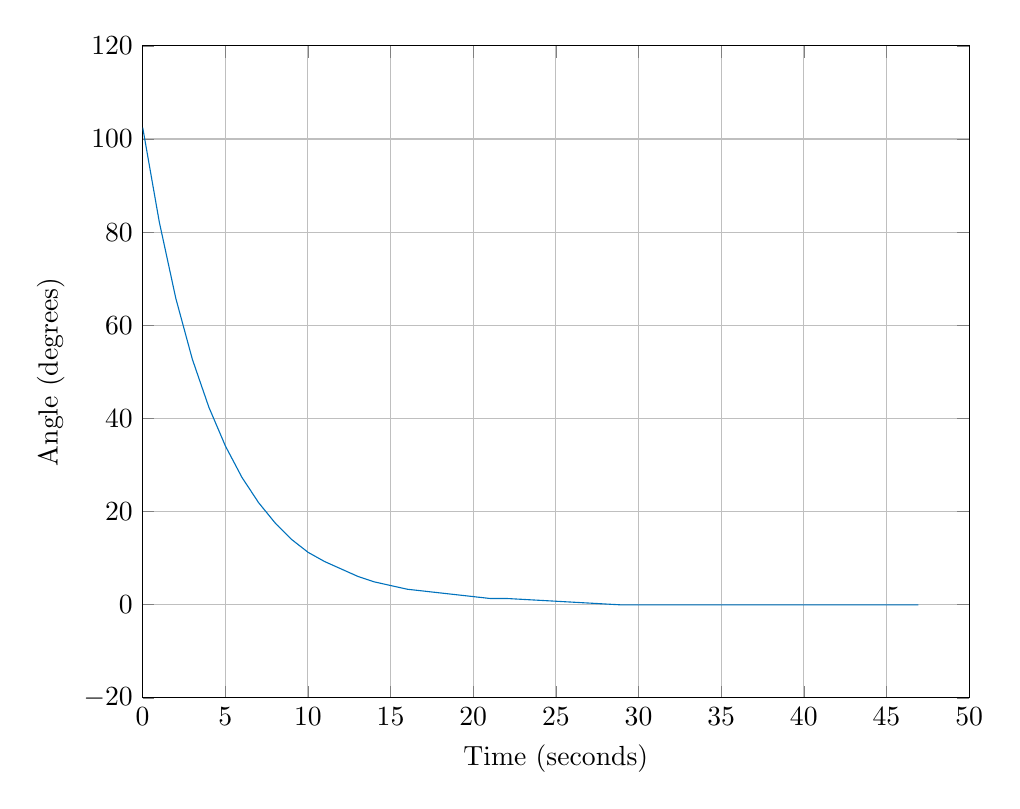
\begin{tikzpicture}

\begin{axis}[%
width=4.133in,
height=3.26in,
at={(0.693in,0.44in)},
scale only axis,
xmin=0,
xmax=50,
xmajorgrids,
xlabel={Time (seconds)},
ymin=-20,
ymax=120,
ymajorgrids,
ylabel={Angle (degrees)},
axis background/.style={fill=white}
]
\addplot [color=mycolor1,solid,forget plot]
  table[row sep=crcr]{%
0	102.4204\\
0.0183688510000007	102.2724\\
0.0333085550000006	101.9604\\
0.048411227	101.6564\\
0.0639306670000004	101.3504\\
0.0799534620000003	101.0264\\
0.0982038640000001	100.6824\\
0.113255477	100.3664\\
0.129045015000001	100.0504\\
0.144356604	99.7204\\
0.160402016	99.4064\\
0.176073557	99.0824\\
0.192149266	98.7664\\
0.207947832	98.4444\\
0.224124653	98.1224\\
0.240001415	97.7964\\
0.258240871	97.4584\\
0.273553052	97.1304\\
0.288614695	96.8164\\
0.303944158	96.4984\\
0.320296693	96.1784\\
0.335924479	95.8584\\
0.351968467	95.5364\\
0.36793271	95.1944\\
0.383990255	94.8784\\
0.400113327000001	94.5564\\
0.416061725	94.2324\\
0.431937103	93.9104\\
0.448054973000001	93.5944\\
0.464105932	93.2704\\
0.480011931	92.9464\\
0.495890924000001	92.6264\\
0.511894759	92.3024\\
0.527906796	91.9764\\
0.543917324000001	91.6544\\
0.560083946	91.3344\\
0.576077847000001	91.0024\\
0.59203282	90.6764\\
0.608008648	90.3544\\
0.624084515000001	90.0344\\
0.639994899	89.7024\\
0.656079034	89.3824\\
0.672099871000001	89.0604\\
0.688106198000001	88.7404\\
0.704106083000001	88.4164\\
0.720049961000001	88.0964\\
0.737160905000001	87.7624\\
0.75250126	87.4444\\
0.768142632999999	87.1244\\
0.784054700999999	86.8004\\
0.800066662	86.4784\\
0.816106512	86.1404\\
0.832087467	85.8204\\
0.848028142000001	85.4864\\
0.864095890000001	85.1744\\
0.880003707	84.8564\\
0.895955854	84.5364\\
0.912117295	84.2144\\
0.928327515000001	83.8904\\
0.94397923	83.5684\\
0.960180325000001	83.2384\\
0.975936496000001	82.9184\\
0.992044641000001	82.5984\\
1.007965717	82.2504\\
1.025603044	81.9724\\
1.040587064	81.7064\\
1.055945238	81.4624\\
1.071973249	81.1984\\
1.088018248	80.9344\\
1.104082485	80.6764\\
1.120156196	80.4164\\
1.136085195	80.1464\\
1.15203761	79.8864\\
1.168089246	79.6264\\
1.183971525	79.3684\\
1.20000799	79.1124\\
1.216084537	78.8444\\
1.232158268	78.5824\\
1.248273158	78.3204\\
1.264076497	78.0584\\
1.280082419	77.7944\\
1.295884334	77.5344\\
1.311956217	77.2604\\
1.328067363	77.0024\\
1.343973684	76.7384\\
1.362448324	76.4684\\
1.377668245	76.2144\\
1.39320529	75.9504\\
1.408662147	75.6884\\
1.424079043	75.4264\\
1.440028938	75.1684\\
1.456163462	74.9064\\
1.47205731	74.6424\\
1.488080376	74.3804\\
1.504082985	74.1204\\
1.520143854	73.8544\\
1.536009798	73.5944\\
1.551891741	73.3284\\
1.568081102	73.0684\\
1.58403343	72.8064\\
1.600087923	72.5344\\
1.616054049	72.2704\\
1.632332509	72.0104\\
1.64787439	71.7384\\
1.663894055	71.4824\\
1.682074156	71.2144\\
1.697872969	70.9584\\
1.713137161	70.7024\\
1.72905725	70.4384\\
1.744443844	70.1764\\
1.760382785	69.9184\\
1.776001737	69.6544\\
1.79198464	69.3924\\
1.808005687	69.1284\\
1.823902869	68.8604\\
1.840012486	68.5884\\
1.856109415	68.3284\\
1.872084489	68.0644\\
1.88811905	67.8044\\
1.904166907	67.5444\\
1.920054249	67.2804\\
1.93609603	67.0244\\
1.95207469	66.7624\\
1.968200148	66.5024\\
1.984080652	66.2424\\
2.000057727	65.9684\\
2.018331214	65.6884\\
2.033306471	65.5024\\
2.048307169	65.3024\\
2.06397708	65.0864\\
2.079933969	64.8844\\
2.09609529	64.6804\\
2.111932893	64.4744\\
2.128148251	64.2644\\
2.144043012	64.0504\\
2.160125172	63.8424\\
2.176089027	63.6344\\
2.192050899	63.4184\\
2.208037105	63.2084\\
2.224094719	63.0004\\
2.24005804	62.7904\\
2.25615572	62.5884\\
2.272046136	62.3724\\
2.287893629	62.1664\\
2.304042884	61.9604\\
2.320069238	61.7504\\
2.336075429	61.5424\\
2.352039902	61.3344\\
2.368128457	61.1264\\
2.384037896	60.9144\\
2.400017871	60.7084\\
2.415924876	60.4944\\
2.432140656	60.2864\\
2.448063229	60.0784\\
2.464108537	59.8704\\
2.480163408	59.6604\\
2.49610458	59.4424\\
2.511973046	59.2384\\
2.528025899	59.0304\\
2.544106219	58.8224\\
2.560032788	58.6144\\
2.576003506	58.4024\\
2.592085312	58.1944\\
2.608035492	57.9764\\
2.624093357	57.7684\\
2.640164633	57.5624\\
2.656125198	57.3584\\
2.672063636	57.1464\\
2.688164912	56.9364\\
2.704155984	56.7284\\
2.720072408	56.5204\\
2.735890672	56.3044\\
2.751870225	56.0964\\
2.770154442	55.8844\\
2.785357205	55.6744\\
2.800494094	55.4704\\
2.816019383	55.2624\\
2.831984091	55.0444\\
2.84801048	54.8404\\
2.864075236	54.6324\\
2.880054037	54.4164\\
2.896098667	54.2124\\
2.912052281	53.9964\\
2.92830805	53.7884\\
2.943932698	53.5824\\
2.962417852	53.3684\\
2.977686605	53.1644\\
2.993616154	52.9584\\
3.009400128	52.7324\\
3.024228897	52.5584\\
3.039919044	52.4024\\
3.055970422	52.2484\\
3.072866972	52.0824\\
3.088017962	51.9204\\
3.103887564	51.7464\\
3.122308995	51.5764\\
3.137616851	51.4124\\
3.15272901	51.2544\\
3.168100655	51.0904\\
3.184029334	50.9264\\
3.199968419	50.7624\\
3.216020495	50.5984\\
3.231953555	50.4284\\
3.248110497	50.2664\\
3.263919455	50.1004\\
3.280095441	49.9384\\
3.295897938	49.7744\\
3.312112208	49.6124\\
3.328019257	49.4424\\
3.343933061	49.2804\\
3.362431593	49.1084\\
3.377549549	48.9464\\
3.392731611	48.7804\\
3.408218288	48.6204\\
3.424109054	48.4544\\
3.440044197	48.2844\\
3.456041296	48.1204\\
3.472079682	47.9584\\
3.487968319	47.7924\\
3.504038273	47.6324\\
3.52001526	47.4644\\
3.536047006	47.2964\\
3.551888667	47.1344\\
3.568106449	46.9684\\
3.584043487	46.8024\\
3.599998716	46.6404\\
3.616067418	46.4684\\
3.632058405	46.3084\\
3.647991444	46.1424\\
3.664075518	45.9804\\
3.680088987	45.8164\\
3.696110265	45.6524\\
3.711984378	45.4884\\
3.728077151	45.3224\\
3.744062864	45.1564\\
3.760323144	44.9924\\
3.776031968	44.8244\\
3.79224752	44.6584\\
3.807954044	44.4944\\
3.824078595	44.3304\\
3.840019811	44.1684\\
3.856091728	44.0024\\
3.872047732	43.8324\\
3.888169813	43.6684\\
3.904113394	43.5004\\
3.920077547	43.3364\\
3.936080613	43.1764\\
3.95203981	43.0144\\
3.968056302	42.8504\\
3.984052371	42.6824\\
4.000004398	42.5184\\
4.018208214	42.3384\\
4.033212486	42.2184\\
4.048166475	42.0904\\
4.064010347	41.9544\\
4.079990957	41.8284\\
4.096028618	41.6904\\
4.112078592	41.5564\\
4.128132431	41.4244\\
4.143971702	41.2944\\
4.160019531	41.1624\\
4.17614748	41.0304\\
4.191983176	40.8984\\
4.207888943	40.7644\\
4.223927622	40.6324\\
4.240118776	40.4984\\
4.256063164	40.3664\\
4.272131016	40.2324\\
4.288157781	40.0984\\
4.303899792	39.9664\\
4.319992519	39.8324\\
4.335995337	39.6984\\
4.351890621	39.5644\\
4.368105944	39.4344\\
4.384069225	39.2984\\
4.400005215	39.1664\\
4.41599692	39.0344\\
4.432103555	38.9024\\
4.448007406	38.7644\\
4.464065191	38.6324\\
4.48006946	38.5004\\
4.496049149	38.3664\\
4.511983417	38.2304\\
4.528015837	38.1024\\
4.544052921	37.9704\\
4.56006316	37.8344\\
4.575976969	37.7004\\
4.594297816	37.5624\\
4.60952331	37.4304\\
4.624655478	37.2984\\
4.640127572	37.1684\\
4.656043469	37.0344\\
4.672049046	36.9024\\
4.688105975	36.7704\\
4.704036732	36.6364\\
4.720056104	36.5044\\
4.736126759	36.3704\\
4.752065218	36.2344\\
4.768082827	36.1004\\
4.786409216	35.9604\\
4.801569694	35.8284\\
4.816685244	35.7004\\
4.834282191	35.5664\\
4.849399359	35.4344\\
4.864709135	35.3024\\
4.88004093	35.1704\\
4.896132682	35.0364\\
4.912002772	34.9044\\
4.928146943	34.7724\\
4.944013909	34.6384\\
4.960076093	34.5044\\
4.976096887	34.3704\\
4.992139772	34.2364\\
5.008023704	34.0984\\
5.025551546	33.9824\\
5.040541056	33.8804\\
5.057022025	33.7764\\
5.072017541	33.6684\\
5.087905034	33.5624\\
5.103991766	33.4484\\
5.120173717	33.3424\\
5.136090723	33.2364\\
5.152037045	33.1284\\
5.168383835	33.0204\\
5.184074633	32.9104\\
5.200121724	32.8064\\
5.216306035	32.6984\\
5.231952102	32.5844\\
5.248089578	32.4804\\
5.264073466	32.3724\\
5.280074507	32.2664\\
5.296065462	32.1584\\
5.31211182	32.0484\\
5.327936899	31.9424\\
5.343977022	31.8364\\
5.36001477	31.7284\\
5.376059974	31.6184\\
5.392059386	31.5104\\
5.407962161	31.4004\\
5.426280871	31.2924\\
5.441475148	31.1864\\
5.456669825	31.0804\\
5.47207129	30.9704\\
5.488115472	30.8664\\
5.504112655	30.7584\\
5.52001728	30.6484\\
5.536034135	30.5364\\
5.551886293	30.4304\\
5.568101255	30.3264\\
5.584075205	30.2164\\
5.600033854	30.1084\\
5.616000594	30.0024\\
5.632115113	29.8944\\
5.648068546	29.7824\\
5.66412602	29.6744\\
5.680021578	29.5684\\
5.696071084	29.4584\\
5.712007269	29.3524\\
5.728144057	29.2464\\
5.744016768	29.1384\\
5.760161989	29.0324\\
5.77604668	28.9204\\
5.791877804	28.8164\\
5.808132852	28.7084\\
5.824030179	28.5984\\
5.840030689	28.4924\\
5.856093851	28.3864\\
5.872014465	28.2724\\
5.888196542	28.1644\\
5.904041825	28.0604\\
5.920048815	27.9504\\
5.936071972	27.8464\\
5.952065726	27.7384\\
5.968085974	27.6284\\
5.984032891	27.5224\\
6.000202233	27.4084\\
6.018186355	27.3004\\
6.03338491	27.2204\\
6.048346837	27.1384\\
6.0639643	27.0464\\
6.079958767	26.9624\\
6.09595861	26.8804\\
6.11203414	26.7964\\
6.128358149	26.7104\\
6.144016052	26.6204\\
6.160255485	26.5364\\
6.176036272	26.4484\\
6.19202431	26.3604\\
6.208006085	26.2764\\
6.224127201	26.1904\\
6.240026174	26.1064\\
6.256046619	26.0164\\
6.272057904	25.9324\\
6.288042101	25.8444\\
6.306266292	25.7524\\
6.321504176	25.6704\\
6.337771502	25.5844\\
6.35283485	25.4984\\
6.368079376	25.4124\\
6.384074635	25.3264\\
6.400105294	25.2424\\
6.416045873	25.1544\\
6.431980675	25.0684\\
6.448071499	24.9844\\
6.464009703	24.9004\\
6.479961941	24.8104\\
6.496096232	24.7224\\
6.512043722	24.6404\\
6.528107449	24.5544\\
6.543868977	24.4664\\
6.562184757	24.3764\\
6.575885431	24.2944\\
6.591889997	24.2084\\
6.608178933	24.1184\\
6.623943859	24.0304\\
6.639935844	23.9484\\
6.655927785	23.8604\\
6.673989082	23.7744\\
6.689320048	23.6884\\
6.705154509	23.6004\\
6.720247033	23.5144\\
6.736071867	23.4284\\
6.75208027	23.3424\\
6.767923657	23.2584\\
6.783989989	23.1684\\
6.80228187	23.0824\\
6.817631854	22.9944\\
6.83292104	22.9124\\
6.848212199	22.8244\\
6.863970204	22.7404\\
6.882241634	22.6504\\
6.897894523	22.5684\\
6.913187308	22.4784\\
6.928397195	22.3964\\
6.943943465	22.3104\\
6.960045764	22.2204\\
6.975865267	22.1344\\
6.992126842	22.0504\\
7.008050062	21.9564\\
7.025718561	21.8824\\
7.040718043	21.8184\\
7.055940243	21.7504\\
7.071948798	21.6804\\
7.087987307	21.6124\\
7.104052907	21.5404\\
7.122582546	21.4684\\
7.137761084	21.3984\\
7.153741457	21.3304\\
7.169128938	21.2604\\
7.184402068	21.1924\\
7.200038639	21.1144\\
7.216094895	21.0464\\
7.232001192	20.9784\\
7.247924525	20.9104\\
7.263997788	20.8424\\
7.279947433	20.7684\\
7.29610655	20.7004\\
7.311906688	20.6324\\
7.328099093	20.5624\\
7.344035714	20.4964\\
7.360078154	20.4224\\
7.376295936	20.3544\\
7.392145454	20.2844\\
7.408146892	20.2144\\
7.424092768	20.1464\\
7.4401449	20.0784\\
7.456162766	20.0064\\
7.472180955	19.9324\\
7.487989538	19.8664\\
7.504052046	19.7984\\
7.520150598	19.7284\\
7.536059701	19.6584\\
7.551890963	19.5904\\
7.568041244	19.5144\\
7.584021531	19.4484\\
7.600051739	19.3784\\
7.616059897	19.3084\\
7.632000233	19.2364\\
7.64813051	19.1684\\
7.66397409	19.1004\\
7.680095258	19.0304\\
7.696049388	18.9624\\
7.712115707	18.8904\\
7.728077525	18.8204\\
7.744041996	18.7524\\
7.760215445	18.6804\\
7.776069825	18.6104\\
7.791990826	18.5384\\
7.808134334	18.4704\\
7.824046704	18.4024\\
7.840095769	18.3304\\
7.855989495	18.2604\\
7.872103104	18.1904\\
7.888161931	18.1224\\
7.904082796	18.0524\\
7.920141037	17.9844\\
7.936030756	17.9124\\
7.952107764	17.8444\\
7.968144938	17.7744\\
7.984028749	17.7024\\
8.000027491	17.6364\\
8.018456827	17.5544\\
8.033437375	17.5064\\
8.048477631	17.4544\\
8.064010218	17.3944\\
8.07994802	17.3384\\
8.096082749	17.2804\\
8.11207047	17.2244\\
8.128055801	17.1684\\
8.143977615	17.1124\\
8.159942048	17.0544\\
8.176176762	17.0004\\
8.19207699	16.9424\\
8.208061404	16.8844\\
8.224100676	16.8264\\
8.240084774	16.7704\\
8.256079355	16.7144\\
8.272108372	16.6544\\
8.288100128	16.5964\\
8.304109482	16.5384\\
8.320065606	16.4844\\
8.3360119	16.4244\\
8.352021506	16.3684\\
8.368085553	16.3144\\
8.384090028	16.2544\\
8.399968159	16.2004\\
8.416119491	16.1424\\
8.432133188	16.0824\\
8.448053146	16.0224\\
8.464013871	15.9704\\
8.480101691	15.9124\\
8.496117539	15.8564\\
8.512068657	15.8004\\
8.528063444	15.7444\\
8.544035171	15.6864\\
8.560087818	15.6284\\
8.575965249	15.5704\\
8.59203178	15.5144\\
8.608116555	15.4564\\
8.624039102	15.4004\\
8.640096362	15.3424\\
8.656076661	15.2844\\
8.672148608	15.2284\\
8.688113748	15.1704\\
8.704000399	15.1144\\
8.722291093	15.0544\\
8.737598975	14.9984\\
8.752907863	14.9424\\
8.768171965	14.8864\\
8.78403743	14.8284\\
8.800054517	14.7704\\
8.816091375	14.7124\\
8.832031724	14.6564\\
8.848089619	14.6024\\
8.864099894	14.5424\\
8.879898027	14.4864\\
8.898206015	14.4244\\
8.913419803	14.3704\\
8.928649112	14.3144\\
8.944309163	14.2564\\
8.960117152	14.2024\\
8.976113348	14.1424\\
8.992105735	14.0844\\
9.008041317	14.0284\\
9.025565869	13.9784\\
9.040568971	13.9364\\
9.055918399	13.8964\\
9.074044499	13.8444\\
9.089062155	13.8044\\
9.104111355	13.7604\\
9.120202733	13.7164\\
9.135847764	13.6704\\
9.154227715	13.6244\\
9.169592449	13.5844\\
9.185173654	13.5344\\
9.200428054	13.4924\\
9.216112278	13.4464\\
9.232056891	13.4064\\
9.248059466	13.3564\\
9.264056213	13.3164\\
9.280137476	13.2724\\
9.296011707	13.2264\\
9.312128554	13.1864\\
9.327894031	13.1364\\
9.343915928	13.0944\\
9.359887763	13.0504\\
9.376304508	13.0064\\
9.392086278	12.9584\\
9.408083651	12.9164\\
9.423885897	12.8704\\
9.440069387	12.8264\\
9.456174895	12.7844\\
9.472077017	12.7344\\
9.488045807	12.6944\\
9.504014724	12.6484\\
9.520117387	12.6064\\
9.536080361	12.5604\\
9.552060696	12.5164\\
9.568192643	12.4744\\
9.584067228	12.4264\\
9.600080837	12.3864\\
9.616080571	12.3364\\
9.632037027	12.2964\\
9.64808969	12.2504\\
9.663998389	12.2064\\
9.680021239	12.1664\\
9.695972707	12.1164\\
9.712047666	12.0724\\
9.728037642	12.0264\\
9.744155183	11.9864\\
9.760088205	11.9384\\
9.776757711	11.8944\\
9.792659794	11.8484\\
9.80796135	11.8064\\
9.824096941	11.7664\\
9.840061966	11.7164\\
9.856077841	11.6744\\
9.872187674	11.6264\\
9.888370271	11.5844\\
9.904031688	11.5404\\
9.92011963	11.4964\\
9.936064576	11.4504\\
9.952094924	11.4064\\
9.968010534	11.3644\\
9.984115427	11.3164\\
10.000072841	11.2744\\
10.018405755	11.2244\\
10.033374081	11.1964\\
10.048361309	11.1664\\
10.063925623	11.1364\\
10.079977202	11.1064\\
10.0959517	11.0744\\
10.11209461	11.0424\\
10.128112962	11.0104\\
10.14433672	10.9784\\
10.160114831	10.9464\\
10.176203033	10.9164\\
10.191977526	10.8864\\
10.208055864	10.8524\\
10.224019291	10.8204\\
10.240103365	10.7864\\
10.256086281	10.7544\\
10.272034549	10.7244\\
10.288105831	10.6944\\
10.304008559	10.6604\\
10.32000401	10.6304\\
10.33607941	10.5984\\
10.35208228	10.5664\\
10.368062094	10.5364\\
10.384037708	10.5044\\
10.399997806	10.4684\\
10.415891448	10.4384\\
10.434147298	10.4064\\
10.449389917	10.3764\\
10.464664212	10.3444\\
10.480136195	10.3124\\
10.496101596	10.2804\\
10.512095791	10.2484\\
10.528197194	10.2184\\
10.544061562	10.1864\\
10.560095223	10.1544\\
10.576334027	10.1224\\
10.592086089	10.0904\\
10.608046754	10.0584\\
10.624091295	10.0284\\
10.640059148	9.99640000000001\\
10.656090181	9.96639999999999\\
10.672056451	9.9324\\
10.688069155	9.8984\\
10.704008368	9.86840000000001\\
10.720175028	9.83839999999999\\
10.736127685	9.8064\\
10.752067162	9.77439999999999\\
10.768036176	9.74039999999999\\
10.784152183	9.7084\\
10.800027295	9.6784\\
10.816082722	9.6464\\
10.832081304	9.6144\\
10.848106229	9.58239999999999\\
10.864075845	9.5504\\
10.880158672	9.5184\\
10.896064783	9.48839999999998\\
10.912086145	9.45639999999999\\
10.928081253	9.4264\\
10.944318274	9.39239999999998\\
10.960121783	9.3604\\
10.976326932	9.32839999999999\\
10.992006523	9.29839999999999\\
11.0080013	9.26439999999999\\
11.025378684	9.24039999999999\\
11.040376159	9.21039999999999\\
11.055933491	9.1904\\
11.074081523	9.1604\\
11.089123683	9.14039999999999\\
11.104067792	9.1104\\
11.120133505	9.08839999999999\\
11.136045394	9.06039999999999\\
11.152107304	9.04040000000001\\
11.168079777	9.01039999999999\\
11.18399414	8.9884\\
11.20004298	8.96039999999999\\
11.216071723	8.93639999999999\\
11.232033611	8.9104\\
11.248089247	8.88239999999999\\
11.264040791	8.8604\\
11.280025518	8.83039999999998\\
11.295892011	8.81039999999999\\
11.314057309	8.7804\\
11.329015801	8.76039999999999\\
11.344009383	8.73039999999999\\
11.359944392	8.7084\\
11.375946781	8.68039999999999\\
11.392062978	8.6584\\
11.408266544	8.63039999999999\\
11.42408148	8.60439999999998\\
11.440146109	8.58039999999998\\
11.456099853	8.55239999999999\\
11.472118214	8.5304\\
11.488105617	8.5004\\
11.504024906	8.47839999999999\\
11.520034221	8.45039999999999\\
11.535874884	8.43039999999999\\
11.554183783	8.40039999999999\\
11.569170447	8.3784\\
11.584171723	8.35039999999999\\
11.59991692	8.32639999999999\\
11.616103331	8.3004\\
11.63203882	8.27239999999999\\
11.648111382	8.2504\\
11.664049792	8.22239999999999\\
11.680107852	8.20039999999999\\
11.696196627	8.1704\\
11.712079884	8.1484\\
11.728120944	8.1204\\
11.744190912	8.10039999999999\\
11.760110975	8.07039999999999\\
11.776241434	8.0504\\
11.792006339	8.0204\\
11.808070405	8.0004\\
11.82391062	7.9704\\
11.840137259	7.9444\\
11.855973512	7.9204\\
11.872005195	7.89439999999999\\
11.888007556	7.8704\\
11.904073667	7.84239999999998\\
11.920119215	7.82039999999999\\
11.935884137	7.79040000000001\\
11.954200807	7.76839999999999\\
11.969444648	7.74039999999999\\
11.984568127	7.7204\\
12.000080963	7.6904\\
12.018308108	7.66239999999999\\
12.033291633	7.64039999999999\\
12.048267951	7.6164\\
12.063930746	7.59039999999999\\
12.079955243	7.56439999999999\\
12.096045491	7.54040000000001\\
12.112087836	7.51239999999999\\
12.128143221	7.49039999999999\\
12.144338367	7.46039999999999\\
12.160052403	7.43839999999999\\
12.176227731	7.4104\\
12.192011332	7.39039999999999\\
12.208090902	7.3604\\
12.224000306	7.34039999999999\\
12.240152174	7.31039999999999\\
12.256107622	7.28639999999999\\
12.272180541	7.26039999999999\\
12.289087141	7.23239999999998\\
12.304143534	7.21039999999999\\
12.319975945	7.1844\\
12.335990792	7.1604\\
12.352122821	7.13239999999999\\
12.368020383	7.1104\\
12.384121135	7.08039999999998\\
12.400066309	7.06039999999999\\
12.416090824	7.0304\\
12.431956683	7.00839999999999\\
12.448094591	6.98039999999999\\
12.46404176	6.95639999999999\\
12.480085964	6.93039999999999\\
12.496019614	6.90439999999998\\
12.512104149	6.88039999999999\\
12.52796677	6.85639999999998\\
12.544008104	6.83039999999998\\
12.560054898	6.8004\\
12.576305451	6.7804\\
12.592105035	6.7504\\
12.608132307	6.73039999999999\\
12.624008253	6.70039999999999\\
12.640036001	6.68039999999999\\
12.65607096	6.65039999999999\\
12.672085016	6.63039999999999\\
12.68809701	6.60039999999999\\
12.704186057	6.58039999999998\\
12.72025265	6.5504\\
12.73603565	6.52239999999999\\
12.752101387	6.5004\\
12.768061065	6.47239999999999\\
12.78403421	6.45039999999999\\
12.79996568	6.4204\\
12.816018772	6.39839999999998\\
12.832095772	6.3704\\
12.848049201	6.35039999999999\\
12.863974919	6.32039999999999\\
12.879994583	6.29839999999999\\
12.896119099	6.2704\\
12.912144415	6.2484\\
12.928095919	6.2204\\
12.944102907	6.1964\\
12.959964465	6.1704\\
12.975945288	6.14239999999998\\
12.993129587	6.1204\\
13.008829587	6.09039999999999\\
13.026328072	6.07039999999999\\
13.041608908	6.05239999999999\\
13.057149056	6.0324\\
13.072211544	6.01439999999999\\
13.08821511	5.9984\\
13.1040371	5.98039999999999\\
13.120026195	5.96039999999999\\
13.135931169	5.9404\\
13.152232144	5.9204\\
13.168052772	5.9024\\
13.184101667	5.88239999999999\\
13.199986184	5.86240000000001\\
13.215908564	5.8424\\
13.232115089	5.8244\\
13.24813843	5.80839999999999\\
13.263986836	5.7884\\
13.280096454	5.76839999999999\\
13.296047911	5.7504\\
13.312143614	5.73039999999999\\
13.328115249	5.7124\\
13.344163292	5.69239999999999\\
13.360135184	5.6724\\
13.376402667	5.6544\\
13.392589307	5.63639999999999\\
13.409157862	5.6164\\
13.424421011	5.59639999999999\\
13.440025529	5.57839999999999\\
13.455966592	5.56039999999999\\
13.472122998	5.54040000000001\\
13.488089952	5.5224\\
13.50407206	5.50239999999999\\
13.520166879	5.48240000000001\\
13.536107394	5.4644\\
13.553903076	5.4444\\
13.569270033	5.42439999999999\\
13.58452683	5.4084\\
13.600041683	5.39039999999999\\
13.615960599	5.3704\\
13.632071672	5.35039999999999\\
13.648105307	5.33039999999998\\
13.66400126	5.3124\\
13.679966004	5.2924\\
13.696039374	5.2704\\
13.712056222	5.2544\\
13.727982176	5.2364\\
13.74388713	5.2184\\
13.762161107	5.19839999999999\\
13.777414329	5.1784\\
13.792662485	5.1604\\
13.808122947	5.14039999999999\\
13.824074175	5.1224\\
13.840156772	5.10239999999999\\
13.856084687	5.08239999999998\\
13.872073323	5.06440000000001\\
13.888114162	5.04639999999999\\
13.904062053	5.0284\\
13.920029496	5.01039999999999\\
13.936069022	4.99039999999999\\
13.952077636	4.9704\\
13.968068529	4.95039999999999\\
13.984112227	4.9324\\
14.000077011	4.91240000000001\\
14.021658944	4.89239999999998\\
14.033776989	4.88239999999999\\
14.048971564	4.87039999999999\\
14.064151972	4.85639999999998\\
14.080082739	4.84439999999999\\
14.096079165	4.83239999999998\\
14.111954885	4.82239999999999\\
14.127983047	4.8064\\
14.146452604	4.7944\\
14.161545208	4.7824\\
14.176746748	4.76839999999999\\
14.193127113	4.7544\\
14.208377274	4.7424\\
14.224087656	4.73039999999999\\
14.240058631	4.7184\\
14.256061041	4.70439999999999\\
14.272094655	4.69239999999999\\
14.288037008	4.68039999999999\\
14.304051043	4.66839999999999\\
14.319986458	4.6544\\
14.33605132	4.64239999999998\\
14.351989841	4.63039999999999\\
14.368031581	4.6144\\
14.384109647	4.60239999999999\\
14.400104539	4.5924\\
14.416066527	4.57839999999999\\
14.432042437	4.56440000000001\\
14.44791576	4.55239999999999\\
14.464054417	4.5424\\
14.480303603	4.5284\\
14.496056951	4.51439999999999\\
14.512053347	4.50239999999999\\
14.528033847	4.49039999999999\\
14.544033306	4.47639999999998\\
14.560068608	4.4624\\
14.576332506	4.45239999999998\\
14.592149429	4.4384\\
14.608079214	4.42439999999999\\
14.624112409	4.4144\\
14.640082159	4.4024\\
14.658217872	4.38639999999999\\
14.673464524	4.37440000000001\\
14.688761816	4.36240000000001\\
14.704003782	4.35239999999999\\
14.720194429	4.33839999999999\\
14.736028902	4.3244\\
14.752112446	4.3124\\
14.768022456	4.30239999999999\\
14.784235387	4.2864\\
14.799879686	4.2744\\
14.816046315	4.26239999999999\\
14.83194389	4.2484\\
14.848077476	4.23440000000001\\
14.864065282	4.22239999999999\\
14.880101759	4.2124\\
14.896034617	4.19839999999999\\
14.912053808	4.18440000000001\\
14.92800523	4.1724\\
14.944266453	4.1604\\
14.960087908	4.14639999999999\\
14.976287221	4.1344\\
14.992705078	4.1224\\
15.008171858	4.1084\\
15.026031547	4.09439999999999\\
15.041078616	4.08439999999999\\
15.056212334	4.07239999999999\\
15.072114697	4.05639999999998\\
15.087996085	4.0444\\
15.104228327	4.0324\\
15.120056448	4.0224\\
15.135974303	4.00839999999999\\
15.15218251	3.99440000000001\\
15.168078228	3.98240000000001\\
15.184083358	3.97239999999999\\
15.200037861	3.95639999999999\\
15.216144813	3.9444\\
15.232057803	3.9324\\
15.248123801	3.91839999999999\\
15.264193253	3.90639999999999\\
15.279983584	3.89239999999998\\
15.295883841	3.88239999999999\\
15.311948992	3.86839999999999\\
15.327913678	3.85439999999998\\
15.343923984	3.8424\\
15.359868792	3.83239999999998\\
15.378277783	3.8164\\
15.393496592	3.80439999999999\\
15.408752721	3.7924\\
15.424126522	3.7784\\
15.439966263	3.76439999999999\\
15.456036015	3.7544\\
15.472152938	3.74039999999999\\
15.488126768	3.72839999999999\\
15.504246238	3.7144\\
15.520001445	3.70239999999998\\
15.536053454	3.69239999999999\\
15.552074135	3.6784\\
15.568034524	3.6644\\
15.584048811	3.6524\\
15.600006908	3.64239999999998\\
15.616114603	3.6264\\
15.632042328	3.61240000000001\\
15.647991154	3.60239999999999\\
15.664015656	3.58839999999999\\
15.680146672	3.57639999999999\\
15.696100683	3.56440000000001\\
15.712140937	3.55239999999999\\
15.728044487	3.5384\\
15.746526748	3.5244\\
15.761945419	3.51239999999999\\
15.777243508	3.5004\\
15.792601092	3.4864\\
15.808000558	3.47439999999999\\
15.824047644	3.4624\\
15.840125564	3.45239999999998\\
15.856011801	3.43640000000001\\
15.87206927	3.42439999999999\\
15.887985038	3.41240000000001\\
15.906436465	3.39639999999999\\
15.921817151	3.3844\\
15.937268666	3.37440000000001\\
15.95250635	3.36240000000001\\
15.968099983	3.3484\\
15.98408341	3.33439999999999\\
16.000033045	3.32239999999999\\
16.019160772	3.31039999999999\\
16.032070861	3.30439999999999\\
16.047950421	3.3004\\
16.064059656	3.2924\\
16.079979152	3.28439999999999\\
16.095955863	3.2804\\
16.112008051	3.2744\\
16.127974299	3.26639999999999\\
16.144211065	3.26039999999999\\
16.159953291	3.2544\\
16.176204252	3.2484\\
16.192008755	3.2424\\
16.208059557	3.23440000000001\\
16.224041641	3.2304\\
16.239967441	3.22439999999999\\
16.2560357	3.2144\\
16.272085246	3.21039999999998\\
16.288009649	3.20439999999999\\
16.304268996	3.1964\\
16.320112515	3.1904\\
16.336049246	3.18440000000001\\
16.352118377	3.18039999999999\\
16.368062665	3.1724\\
16.384100399	3.1644\\
16.400039164	3.16040000000001\\
16.415905155	3.1524\\
16.432038321	3.14639999999999\\
16.448083251	3.14039999999999\\
16.464002112	3.1344\\
16.480063565	3.1284\\
16.495973104	3.1224\\
16.512272175	3.1144\\
16.528064233	3.1104\\
16.54410943	3.10239999999999\\
16.560020803	3.09439999999999\\
16.576095432	3.0904\\
16.592006636	3.08439999999999\\
16.608131927	3.07639999999999\\
16.623921351	3.07039999999999\\
16.640018506	3.06440000000001\\
16.65587196	3.05839999999999\\
16.671922535	3.05239999999999\\
16.688033103	3.0444\\
16.704273892	3.04040000000001\\
16.720145265	3.03439999999999\\
16.736015581	3.0244\\
16.752101444	3.02039999999998\\
16.768044153	3.01439999999999\\
16.783983009	3.0064\\
16.799973296	3.0004\\
16.816089643	2.99440000000001\\
16.832052814	2.9884\\
16.847976177	2.98240000000001\\
16.864055714	2.97439999999999\\
16.880134697	2.9704\\
16.8960682	2.9644\\
16.912202809	2.95439999999999\\
16.927988643	2.95039999999999\\
16.944314695	2.9444\\
16.960026963	2.93640000000001\\
16.976195142	2.9324\\
16.99200729	2.92439999999999\\
17.007993784	2.91839999999999\\
17.024039507	2.91240000000001\\
17.039916763	2.9044\\
17.05607475	2.90039999999998\\
17.072240064	2.89439999999999\\
17.088102689	2.8844\\
17.104174483	2.88039999999999\\
17.120067505	2.87440000000001\\
17.135995201	2.86839999999999\\
17.152065172	2.86240000000001\\
17.168019809	2.85439999999998\\
17.184004992	2.85039999999999\\
17.200055638	2.8424\\
17.216090424	2.83439999999999\\
17.232048534	2.83039999999998\\
17.248068048	2.8244\\
17.264147643	2.8164\\
17.280050306	2.81039999999999\\
17.295882453	2.80439999999999\\
17.314005619	2.79639999999999\\
17.32923869	2.7924\\
17.344601115	2.78439999999999\\
17.359974494	2.7804\\
17.376140642	2.7744\\
17.39196678	2.76439999999999\\
17.408035314	2.76039999999999\\
17.424012807	2.7544\\
17.440038397	2.74640000000001\\
17.456094703	2.74039999999999\\
17.4720571	2.73440000000001\\
17.48805083	2.72839999999999\\
17.5042742	2.72239999999999\\
17.5200809	2.7144\\
17.535932084	2.70839999999998\\
17.55428642	2.70439999999999\\
17.569387392	2.6944\\
17.584582433	2.6904\\
17.600132242	2.68440000000001\\
17.615927609	2.6764\\
17.632068929	2.6704\\
17.64809296	2.6644\\
17.664035995	2.66040000000001\\
17.680121483	2.65039999999998\\
17.696032901	2.64439999999999\\
17.711998422	2.64039999999999\\
17.728014298	2.6344\\
17.74438901	2.6264\\
17.760033078	2.62039999999999\\
17.776110848	2.6144\\
17.792230062	2.6084\\
17.808112317	2.60239999999999\\
17.824066622	2.59439999999999\\
17.839987086	2.5904\\
17.856013763	2.58239999999998\\
17.871946753	2.5744\\
17.888089334	2.57039999999999\\
17.904110458	2.56440000000001\\
17.919946757	2.5564\\
17.935995933	2.5504\\
17.951922463	2.5444\\
17.967969661	2.5384\\
17.984104741	2.5324\\
18.000042354	2.5244\\
18.018661637	2.51839999999999\\
18.03393537	2.51239999999999\\
18.049139241	2.5044\\
18.06421122	2.5004\\
18.080157826	2.49440000000001\\
18.095921635	2.4864\\
18.111956488	2.4804\\
18.128070841	2.47439999999999\\
18.144100843	2.4684\\
18.160067361	2.4624\\
18.176072322	2.45439999999999\\
18.192008452	2.45039999999999\\
18.207894441	2.4444\\
18.224031826	2.43440000000001\\
18.240088559	2.43039999999999\\
18.255945224	2.42439999999999\\
18.272043849	2.4164\\
18.288187723	2.41240000000001\\
18.304225694	2.4044\\
18.319979197	2.39839999999998\\
18.338144405	2.39239999999998\\
18.353388632	2.3844\\
18.368685694	2.38039999999999\\
18.385926168	2.37440000000001\\
18.401264949	2.3664\\
18.416769812	2.3604\\
18.432070967	2.35439999999998\\
18.448175278	2.3484\\
18.464050569	2.3424\\
18.480119098	2.33439999999999\\
18.496058275	2.33039999999998\\
18.511924205	2.32239999999999\\
18.52814654	2.31440000000001\\
18.544009012	2.31039999999999\\
18.560110449	2.30439999999999\\
18.576289979	2.29639999999999\\
18.591956296	2.29040000000001\\
18.608061686	2.28439999999999\\
18.624045313	2.2784\\
18.640011425	2.2724\\
18.656035308	2.26439999999999\\
18.672082825	2.26039999999999\\
18.68793446	2.2544\\
18.704150892	2.24440000000001\\
18.720110817	2.24039999999999\\
18.736021903	2.23440000000001\\
18.751881791	2.22639999999998\\
18.7678851	2.2204\\
18.784104607	2.2144\\
18.79992235	2.20839999999998\\
18.816038035	2.20239999999998\\
18.832030272	2.1944\\
18.848089107	2.1904\\
18.864149183	2.18440000000001\\
18.880072002	2.17439999999999\\
18.895961443	2.1704\\
18.912073229	2.1644\\
18.928090725	2.15639999999999\\
18.944031888	2.15039999999998\\
18.959962204	2.14439999999999\\
18.976158718	2.13839999999999\\
18.992004307	2.13239999999999\\
19.008185971	2.12440000000001\\
19.025573896	2.12039999999999\\
19.0412209	2.1144\\
19.056318062	2.10439999999998\\
19.072227348	2.10039999999999\\
19.087925621	2.09439999999999\\
19.104166508	2.08839999999999\\
19.119916739	2.08239999999998\\
19.135850792	2.0744\\
19.154169908	2.0684\\
19.169308541	2.0624\\
19.184418173	2.05439999999999\\
19.200025553	2.0504\\
19.216122004	2.0444\\
19.232050041	2.0364\\
19.247997237	2.0304\\
19.264037078	2.0244\\
19.279972581	2.01839999999999\\
19.296055778	2.01239999999999\\
19.314533459	2.0044\\
19.329742691	2.0004\\
19.344987813	1.99440000000001\\
19.360292237	1.98440000000001\\
19.376003727	1.9804\\
19.392059122	1.97439999999999\\
19.408037647	1.96639999999999\\
19.423992775	1.96039999999998\\
19.43996003	1.95439999999999\\
19.455970413	1.94839999999999\\
19.472088003	1.94239999999999\\
19.488185655	1.93440000000001\\
19.504078594	1.93039999999999\\
19.520072996	1.92439999999999\\
19.5361104	1.9144\\
19.551931428	1.91040000000001\\
19.567888699	1.9044\\
19.584126956	1.89639999999999\\
19.600038347	1.89039999999999\\
19.616055456	1.8844\\
19.632039944	1.8784\\
19.648112092	1.8724\\
19.6640722	1.8644\\
19.679990411	1.8604\\
19.696210577	1.85439999999998\\
19.712227061	1.84639999999999\\
19.728084495	1.8404\\
19.744294824	1.83439999999999\\
19.760063177	1.82639999999999\\
19.776087426	1.82039999999999\\
19.792016867	1.81440000000001\\
19.808085707	1.81039999999999\\
19.824029249	1.80239999999999\\
19.840014527	1.7944\\
19.856051171	1.79040000000001\\
19.872124456	1.78439999999999\\
19.888036929	1.7764\\
19.904201072	1.77039999999998\\
19.920024154	1.76439999999999\\
19.936031473	1.75839999999999\\
19.952138348	1.75239999999999\\
19.967962173	1.74440000000001\\
19.984093248	1.74039999999999\\
19.999984341	1.73240000000001\\
20.018235427	1.72439999999999\\
20.033398976	1.7204\\
20.048479309	1.7144\\
20.064103367	1.70639999999999\\
20.080060498	1.70039999999999\\
20.096034048	1.6944\\
20.112224814	1.6884\\
20.127986443	1.6824\\
20.143986276	1.67439999999999\\
20.159981733	1.6704\\
20.17629535	1.6644\\
20.191998826	1.6544\\
20.208061538	1.65039999999998\\
20.223980448	1.64439999999999\\
20.239969492	1.63639999999999\\
20.256054504	1.63039999999999\\
20.272159972	1.62440000000001\\
20.287967588	1.62039999999999\\
20.306222091	1.61240000000001\\
20.321433374	1.60439999999998\\
20.336587557	1.60039999999999\\
20.352152305	1.59439999999999\\
20.368015543	1.58439999999999\\
20.384078445	1.58039999999998\\
20.400042363	1.5744\\
20.416095913	1.5684\\
20.43206209	1.5624\\
20.448153637	1.55439999999999\\
20.464152219	1.5504\\
20.480013522	1.5424\\
20.496097552	1.53439999999999\\
20.512152031	1.5304\\
20.528082706	1.5244\\
20.54396704	1.51639999999999\\
20.559968864	1.51039999999999\\
20.576131594	1.5044\\
20.592072915	1.4984\\
20.608044715	1.4924\\
20.623994312	1.48440000000001\\
20.640304624	1.4804\\
20.65589583	1.47439999999999\\
20.671875286	1.4644\\
20.688083964	1.46039999999998\\
20.704099283	1.45439999999999\\
20.72014689	1.4464\\
20.736018315	1.4404\\
20.752060788	1.43440000000001\\
20.76803986	1.4284\\
20.784088864	1.4224\\
20.800041997	1.4144\\
20.816140715	1.41040000000001\\
20.832077976	1.4044\\
20.848087718	1.39439999999999\\
20.86403155	1.39039999999999\\
20.879896504	1.3844\\
20.896036108	1.3764\\
20.912068512	1.37039999999999\\
20.928018422	1.3644\\
20.944086309	1.3584\\
20.960040379	1.35239999999999\\
20.976085297	1.34439999999999\\
20.992071939	1.3404\\
21.008075045	1.33439999999999\\
21.026015658	1.33239999999998\\
21.041163116	1.33239999999998\\
21.056209224	1.33239999999998\\
21.072067163	1.33239999999998\\
21.088009917	1.33239999999998\\
21.104185023	1.33239999999998\\
21.119975772	1.33239999999998\\
21.136008317	1.33239999999998\\
21.152069373	1.33239999999998\\
21.168069337	1.33239999999998\\
21.184081514	1.33239999999998\\
21.200044283	1.33239999999998\\
21.215987813	1.33239999999998\\
21.232074149	1.33239999999998\\
21.248084544	1.33239999999998\\
21.264099575	1.33239999999998\\
21.280093801	1.33239999999998\\
21.298414903	1.33239999999998\\
21.313482647	1.33239999999998\\
21.328762004	1.33239999999998\\
21.34489592	1.33239999999998\\
21.360044223	1.33239999999998\\
21.376062795	1.33239999999998\\
21.39203227	1.33239999999998\\
21.408168296	1.33239999999998\\
21.423936554	1.33239999999998\\
21.440129151	1.33239999999998\\
21.456051875	1.33239999999998\\
21.472107886	1.33239999999998\\
21.488080395	1.33239999999998\\
21.50398275	1.33239999999998\\
21.520112969	1.33239999999998\\
21.535884545	1.33239999999998\\
21.552121117	1.33239999999998\\
21.568065559	1.33239999999998\\
21.58411713	1.33239999999998\\
21.600049254	1.33239999999998\\
21.616118772	1.33239999999998\\
21.632026667	1.33239999999998\\
21.648058353	1.33239999999998\\
21.664078477	1.33239999999998\\
21.680072523	1.33239999999998\\
21.695937271	1.33239999999998\\
21.711969888	1.33239999999998\\
21.728046075	1.33239999999998\\
21.746503731	1.33239999999998\\
21.761785909	1.33239999999998\\
21.776991583	1.33239999999998\\
21.792411076	1.33239999999998\\
21.808087965	1.33239999999998\\
21.823874124	1.33239999999998\\
21.839897309	1.33239999999998\\
21.855972726	1.33239999999998\\
21.872094822	1.33239999999998\\
21.888049028	1.33239999999998\\
21.904145946	1.33239999999998\\
21.920020395	1.33239999999998\\
21.936095003	1.33239999999998\\
21.952077267	1.33239999999998\\
21.968175289	1.33239999999998\\
21.984522513	1.33239999999998\\
22.000060619	1.33239999999998\\
22.018158303	1.33039999999998\\
22.033488012	1.32639999999999\\
22.048459011	1.3244\\
22.06404852	1.32039999999999\\
22.080208227	1.3164\\
22.09608663	1.31440000000001\\
22.112081747	1.31039999999999\\
22.127969462	1.30639999999998\\
22.144040038	1.30439999999999\\
22.159943269	1.3004\\
22.176284829	1.29839999999999\\
22.192049064	1.29639999999999\\
22.208085811	1.2944\\
22.224080315	1.2884\\
22.240054203	1.2864\\
22.256076923	1.28439999999999\\
22.272092778	1.2804\\
22.288024352	1.2764\\
22.303894411	1.2744\\
22.319981029	1.27039999999998\\
22.336093601	1.26639999999999\\
22.352103953	1.26439999999999\\
22.368042533	1.26039999999999\\
22.384133739	1.2564\\
22.400096143	1.2544\\
22.416215634	1.2504\\
22.43200576	1.24640000000001\\
22.448049384	1.24440000000001\\
22.464051201	1.24039999999999\\
22.480144111	1.2384\\
22.496142106	1.23440000000001\\
22.512058495	1.23240000000001\\
22.528260246	1.22839999999999\\
22.544052714	1.22639999999998\\
22.559998541	1.22439999999999\\
22.576205793	1.2184\\
22.59202278	1.21639999999999\\
22.607954685	1.2144\\
22.623980337	1.21039999999998\\
22.640096123	1.20639999999999\\
22.656147829	1.20439999999999\\
22.672006703	1.20039999999999\\
22.688092874	1.1964\\
22.704107891	1.1944\\
22.720036563	1.1904\\
22.738238104	1.18640000000001\\
22.753421225	1.18440000000001\\
22.76872533	1.18039999999999\\
22.784146561	1.17639999999999\\
22.800052194	1.17439999999999\\
22.815987516	1.1704\\
22.832189616	1.16839999999999\\
22.84791287	1.1664\\
22.864010956	1.1644\\
22.880110702	1.1584\\
22.895954744	1.15639999999999\\
22.912075966	1.1544\\
22.928008061	1.15039999999998\\
22.943982398	1.14639999999999\\
22.960190773	1.14439999999999\\
22.976028864	1.14039999999999\\
22.992021959	1.13639999999999\\
23.008131977	1.1344\\
23.025820927	1.13039999999999\\
23.04107414	1.1264\\
23.056149461	1.12440000000001\\
23.072064682	1.12039999999999\\
23.088100804	1.1164\\
23.104092356	1.1144\\
23.120149976	1.1104\\
23.136090602	1.10839999999999\\
23.152052242	1.10439999999998\\
23.168067276	1.10239999999999\\
23.184064588	1.0984\\
23.200077361	1.09639999999999\\
23.216502654	1.09439999999999\\
23.23207552	1.08839999999998\\
23.248070994	1.08639999999998\\
23.264068116	1.08439999999999\\
23.279893054	1.08039999999998\\
23.295915107	1.07639999999999\\
23.312080723	1.0744\\
23.328028642	1.07039999999999\\
23.344059687	1.0664\\
23.36011691	1.06440000000001\\
23.375963578	1.06039999999999\\
23.392144782	1.05639999999998\\
23.408058055	1.05439999999999\\
23.424065177	1.0504\\
23.440034139	1.04639999999999\\
23.456076664	1.0444\\
23.47203507	1.04040000000001\\
23.48807329	1.0364\\
23.504108017	1.0364\\
23.52008727	1.03439999999999\\
23.536001023	1.0284\\
23.552084193	1.0264\\
23.568030427	1.0244\\
23.584004623	1.02039999999998\\
23.600078771	1.01639999999999\\
23.616058318	1.01439999999999\\
23.632081138	1.01039999999999\\
23.64786872	1.0064\\
23.663912769	1.0044\\
23.680007689	1.0004\\
23.696097208	0.996400000000008\\
23.712067994	0.994400000000013\\
23.728103458	0.990399999999994\\
23.744002408	0.986400000000003\\
23.762446153	0.984400000000008\\
23.777752265	0.980400000000003\\
23.79294696	0.978399999999993\\
23.808178215	0.974399999999989\\
23.823994065	0.972399999999993\\
23.840097929	0.968400000000003\\
23.856091849	0.966399999999993\\
23.872027203	0.964399999999998\\
23.88808883	0.958399999999983\\
23.904036009	0.956399999999988\\
23.920043415	0.954399999999993\\
23.936391688	0.950399999999988\\
23.953060914	0.946399999999997\\
23.96850362	0.944400000000002\\
23.984046886	0.940399999999997\\
24.000091119	0.936400000000006\\
24.01924402	0.934400000000011\\
24.031987124	0.930399999999992\\
24.048000035	0.926399999999987\\
24.063955726	0.924399999999991\\
24.079938336	0.920400000000001\\
24.095971888	0.916399999999996\\
24.112097251	0.914400000000001\\
24.128193418	0.91040000000001\\
24.144026022	0.9084\\
24.160093605	0.906399999999991\\
24.176117257	0.904399999999995\\
24.192122037	0.898399999999981\\
24.208310098	0.896399999999986\\
24.224084976	0.89439999999999\\
24.240132252	0.88839999999999\\
24.256771867	0.886399999999995\\
24.272087256	0.884399999999999\\
24.287924669	0.880399999999995\\
24.303897846	0.876400000000004\\
24.319947608	0.874400000000009\\
24.336100735	0.870399999999989\\
24.352015556	0.866399999999999\\
24.368112743	0.864400000000003\\
24.384091659	0.860399999999998\\
24.400086574	0.856399999999979\\
24.415877955	0.854399999999984\\
24.434031032	0.850399999999993\\
24.4491764	0.846399999999988\\
24.464329225	0.844399999999993\\
24.479885865	0.840400000000002\\
24.496056185	0.838399999999979\\
24.512110732	0.836399999999983\\
24.527953367	0.834399999999988\\
24.544158403	0.828399999999988\\
24.560313754	0.826399999999992\\
24.576072041	0.824399999999997\\
24.592137047	0.820399999999992\\
24.608088235	0.816400000000002\\
24.624014751	0.814400000000006\\
24.640121275	0.810399999999987\\
24.656074551	0.806399999999982\\
24.672078307	0.804399999999987\\
24.688209901	0.800399999999996\\
24.704135702	0.796399999999991\\
24.720134483	0.794399999999996\\
24.736009484	0.790400000000005\\
24.751987293	0.7864\\
24.768068486	0.784399999999991\\
24.783994126	0.7804\\
24.802276965	0.778400000000005\\
24.817502456	0.776399999999995\\
24.833007354	0.7744\\
24.848220926	0.768399999999986\\
24.864036227	0.76639999999999\\
24.880026582	0.764399999999995\\
24.895984966	0.76039999999999\\
24.912219835	0.756399999999999\\
24.928119056	0.754400000000004\\
24.943955361	0.750399999999999\\
24.962368003	0.746400000000008\\
24.977481494	0.744400000000013\\
24.992552804	0.740399999999994\\
25.008080839	0.736400000000003\\
25.025675821	0.734400000000008\\
25.040792011	0.730400000000003\\
25.055937519	0.726399999999984\\
25.072087079	0.724399999999989\\
25.088087555	0.720399999999998\\
25.104077821	0.716399999999993\\
25.120078347	0.714399999999998\\
25.136050905	0.712400000000002\\
25.151984235	0.708399999999983\\
25.168174616	0.706399999999988\\
25.18413209	0.704399999999993\\
25.20031128	0.698399999999992\\
25.216024649	0.696399999999997\\
25.232086518	0.694400000000002\\
25.247967571	0.690399999999997\\
25.264088636	0.686400000000006\\
25.280238258	0.684400000000011\\
25.295959289	0.680399999999992\\
25.312104339	0.676399999999987\\
25.328104708	0.674399999999991\\
25.344075678	0.670400000000001\\
25.360279959	0.666399999999996\\
25.376085432	0.664400000000001\\
25.392064854	0.66040000000001\\
25.408016775	0.656399999999991\\
25.424062637	0.654399999999995\\
25.440082532	0.650399999999976\\
25.456103849	0.646399999999986\\
25.472074973	0.646399999999986\\
25.488068627	0.64439999999999\\
25.504167705	0.63839999999999\\
25.52006643	0.636399999999995\\
25.535954338	0.634399999999999\\
25.552033594	0.628399999999999\\
25.568072271	0.626400000000004\\
25.584056026	0.624400000000009\\
25.600076453	0.620399999999989\\
25.61606208	0.616399999999999\\
25.632117624	0.614400000000003\\
25.648039907	0.610399999999998\\
25.663905129	0.606399999999979\\
25.679935421	0.604399999999984\\
25.695930657	0.600399999999993\\
25.712066915	0.596399999999988\\
25.728234744	0.594399999999993\\
25.744106327	0.590400000000002\\
25.760151911	0.588399999999979\\
25.776063184	0.584399999999988\\
25.791923722	0.580399999999983\\
25.810169382	0.578399999999988\\
25.825448352	0.576399999999992\\
25.841544433	0.574399999999997\\
25.856699839	0.568399999999997\\
25.872095759	0.566400000000002\\
25.888066358	0.564400000000006\\
25.904177037	0.560399999999987\\
25.920049271	0.556399999999982\\
25.936082697	0.554399999999987\\
25.952057845	0.550399999999996\\
25.968136562	0.546399999999991\\
25.984037517	0.544399999999996\\
26.000069926	0.540400000000005\\
26.018211514	0.5364\\
26.033439168	0.534399999999991\\
26.048739727	0.5304\\
26.063888513	0.526399999999995\\
26.080091317	0.5244\\
26.09607858	0.520399999999981\\
26.112110225	0.518399999999986\\
26.12811996	0.51639999999999\\
26.144066954	0.512399999999985\\
26.160177863	0.508399999999995\\
26.176072609	0.506399999999999\\
26.192019265	0.504400000000004\\
26.208018115	0.498400000000004\\
26.224130803	0.496400000000008\\
26.240076179	0.494400000000013\\
26.256079544	0.490399999999994\\
26.271955447	0.486400000000003\\
26.288078711	0.484400000000008\\
26.304180452	0.480400000000003\\
26.320053525	0.476399999999984\\
26.336054488	0.474399999999989\\
26.352036066	0.470399999999998\\
26.368081403	0.466399999999993\\
26.384115063	0.464399999999998\\
26.399984062	0.460399999999979\\
26.416038312	0.456399999999988\\
26.432126626	0.454399999999993\\
26.448072903	0.452399999999983\\
26.464097155	0.448399999999992\\
26.480050696	0.446399999999997\\
26.496074273	0.444400000000002\\
26.512056773	0.438400000000001\\
26.530439384	0.436400000000006\\
26.545791745	0.434400000000011\\
26.560926177	0.428399999999996\\
26.576256032	0.426399999999987\\
26.592206676	0.424399999999991\\
26.608086359	0.420400000000001\\
26.624074501	0.416399999999996\\
26.640089815	0.414400000000001\\
26.656105349	0.41040000000001\\
26.672067798	0.406399999999991\\
26.68808425	0.404399999999995\\
26.704085992	0.400399999999976\\
26.720046532	0.396399999999986\\
26.736082429	0.39439999999999\\
26.752033255	0.390399999999985\\
26.768067502	0.38839999999999\\
26.784167021	0.386399999999995\\
26.800222656	0.384399999999999\\
26.816195408	0.378399999999999\\
26.832074303	0.376400000000004\\
26.848106786	0.374400000000009\\
26.864077754	0.368399999999994\\
26.879996108	0.366399999999999\\
26.896049137	0.364400000000003\\
26.912090539	0.360399999999998\\
26.928131131	0.356399999999979\\
26.944000008	0.354399999999984\\
26.95999141	0.350399999999993\\
26.976112897	0.346399999999988\\
26.99451382	0.344399999999993\\
27.00982589	0.340400000000002\\
27.025727631	0.336399999999983\\
27.041169454	0.334399999999988\\
27.057428988	0.330399999999983\\
27.071966897	0.326399999999992\\
27.088005103	0.324399999999997\\
27.104206596	0.322399999999988\\
27.119951497	0.318399999999997\\
27.136073167	0.316400000000002\\
27.152078603	0.314400000000006\\
27.16791146	0.308399999999992\\
27.184122044	0.306399999999982\\
27.200108754	0.304399999999987\\
27.216056119	0.300399999999996\\
27.232119691	0.296399999999991\\
27.247997289	0.294399999999996\\
27.264101288	0.290400000000005\\
27.280071194	0.2864\\
27.296055177	0.284399999999991\\
27.312470707	0.2804\\
27.327896901	0.276399999999995\\
27.343874722	0.2744\\
27.360224525	0.270399999999981\\
27.376030241	0.26639999999999\\
27.391993894	0.264399999999995\\
27.408049502	0.26039999999999\\
27.423995481	0.258399999999995\\
27.440051745	0.256399999999999\\
27.456151645	0.252399999999994\\
27.47206122	0.248400000000004\\
27.488077467	0.246400000000008\\
27.504081879	0.244400000000013\\
27.520108599	0.238399999999999\\
27.5360765	0.236400000000003\\
27.552030545	0.234400000000008\\
27.568369778	0.230400000000003\\
27.584122787	0.226399999999984\\
27.600804916	0.224399999999989\\
27.616107025	0.220399999999998\\
27.632123471	0.216399999999993\\
27.648198844	0.214399999999998\\
27.664109186	0.210399999999979\\
27.680069019	0.206399999999988\\
27.696073759	0.204399999999993\\
27.712085565	0.200399999999988\\
27.728165272	0.196399999999997\\
27.743990903	0.194400000000002\\
27.762433766	0.192399999999992\\
27.777745331	0.188400000000001\\
27.792980933	0.186400000000006\\
27.808147164	0.184400000000011\\
27.824062731	0.178399999999996\\
27.839994257	0.176399999999987\\
27.85618221	0.174399999999991\\
27.872089219	0.170400000000001\\
27.888035542	0.166399999999996\\
27.904112379	0.164400000000001\\
27.92013558	0.16040000000001\\
27.936200411	0.156399999999991\\
27.9520649	0.154399999999995\\
27.968112954	0.150399999999976\\
27.984047329	0.146399999999986\\
28.00012428	0.14439999999999\\
28.018312195	0.140399999999985\\
28.032070823	0.136399999999995\\
28.047931665	0.134399999999999\\
28.064097624	0.130399999999995\\
28.079986739	0.128399999999999\\
28.096131295	0.124400000000009\\
28.11210098	0.122399999999999\\
28.128130557	0.118399999999994\\
28.144113838	0.116399999999999\\
28.160331825	0.114400000000003\\
28.176159685	0.108399999999989\\
28.19208533	0.106399999999979\\
28.208080784	0.104399999999984\\
28.224043959	0.100399999999993\\
28.240073827	0.0963999999999885\\
28.256099182	0.0943999999999932\\
28.271970131	0.0904000000000025\\
28.28822913	0.0863999999999834\\
28.303947989	0.084399999999988\\
28.320041684	0.0803999999999832\\
28.336029564	0.0763999999999925\\
28.352071424	0.0743999999999971\\
28.368123826	0.0703999999999922\\
28.384089332	0.0664000000000016\\
28.400050348	0.0644000000000062\\
28.41592413	0.0603999999999871\\
28.432132683	0.0583999999999918\\
28.448001978	0.0563999999999822\\
28.464073261	0.0543999999999869\\
28.480132001	0.0483999999999867\\
28.496098507	0.0463999999999913\\
28.512116679	0.044399999999996\\
28.528066224	0.0404000000000053\\
28.544068591	0.0364000000000004\\
28.560277528	0.0343999999999909\\
28.575907348	0.0304000000000002\\
28.594288101	0.0263999999999953\\
28.60942962	0.0244\\
28.624585126	0.0203999999999951\\
28.640030008	0.0164000000000044\\
28.656076393	0.0143999999999949\\
28.672702385	0.0104000000000042\\
28.688100574	0.00639999999998508\\
28.704079165	0.00439999999998975\\
28.720085722	0.000399999999984857\\
28.736043377	-0.00160000000001048\\
28.752041662	-0.00360000000000582\\
28.768080384	-0.00560000000000116\\
28.784088687	-0.0116000000000014\\
28.799908908	-0.0135999999999967\\
28.816191505	-0.0155999999999921\\
28.831943892	-0.0216000000000065\\
28.847873589	-0.0236000000000161\\
28.863970223	-0.0256000000000114\\
28.879931395	-0.0296000000000021\\
28.896067331	-0.033600000000007\\
28.912068594	-0.0356000000000023\\
28.928100069	-0.0396000000000214\\
28.944093237	-0.0436000000000121\\
28.960240173	-0.0456000000000074\\
28.976105363	-0.0496000000000123\\
28.99232086	-0.053600000000003\\
29.008094759	-0.053600000000003\\
29.025572679	-0.053600000000003\\
29.041499492	-0.053600000000003\\
29.056647766	-0.053600000000003\\
29.072175937	-0.053600000000003\\
29.087890915	-0.053600000000003\\
29.104089454	-0.053600000000003\\
29.120144528	-0.053600000000003\\
29.136083619	-0.053600000000003\\
29.152098041	-0.053600000000003\\
29.168074955	-0.053600000000003\\
29.184060143	-0.053600000000003\\
29.200086642	-0.053600000000003\\
29.216061348	-0.053600000000003\\
29.231955916	-0.053600000000003\\
29.248265166	-0.053600000000003\\
29.264140488	-0.053600000000003\\
29.280038112	-0.053600000000003\\
29.295881591	-0.053600000000003\\
29.312378802	-0.053600000000003\\
29.32808617	-0.053600000000003\\
29.344030226	-0.053600000000003\\
29.360278332	-0.053600000000003\\
29.376155127	-0.053600000000003\\
29.392164372	-0.053600000000003\\
29.411405706	-0.053600000000003\\
29.424667021	-0.053600000000003\\
29.439902203	-0.053600000000003\\
29.456131177	-0.053600000000003\\
29.472085543	-0.053600000000003\\
29.488215521	-0.053600000000003\\
29.504099783	-0.053600000000003\\
29.520000383	-0.053600000000003\\
29.536029031	-0.053600000000003\\
29.552111231	-0.053600000000003\\
29.568114264	-0.053600000000003\\
29.584078178	-0.053600000000003\\
29.600172121	-0.053600000000003\\
29.615996221	-0.053600000000003\\
29.632200683	-0.053600000000003\\
29.648094608	-0.053600000000003\\
29.664028025	-0.053600000000003\\
29.679979955	-0.053600000000003\\
29.695979253	-0.053600000000003\\
29.712043272	-0.053600000000003\\
29.728224442	-0.053600000000003\\
29.744013779	-0.053600000000003\\
29.760048324	-0.053600000000003\\
29.776090912	-0.053600000000003\\
29.792119274	-0.053600000000003\\
29.80804948	-0.053600000000003\\
29.824138666	-0.053600000000003\\
29.840020983	-0.053600000000003\\
29.85615446	-0.053600000000003\\
29.871959465	-0.053600000000003\\
29.890530095	-0.053600000000003\\
29.904084111	-0.053600000000003\\
29.920006757	-0.053600000000003\\
29.936087308	-0.053600000000003\\
29.952029842	-0.053600000000003\\
29.96810671	-0.053600000000003\\
29.984073649	-0.053600000000003\\
30.000118831	-0.053600000000003\\
30.01846943	-0.053600000000003\\
30.034081328	-0.053600000000003\\
30.049513748	-0.053600000000003\\
30.064680213	-0.053600000000003\\
30.079926177	-0.053600000000003\\
30.095889678	-0.053600000000003\\
30.112090455	-0.053600000000003\\
30.128140392	-0.053600000000003\\
30.144248583	-0.053600000000003\\
30.160323547	-0.053600000000003\\
30.176179086	-0.053600000000003\\
30.192105384	-0.053600000000003\\
30.208035023	-0.053600000000003\\
30.224087551	-0.053600000000003\\
30.240068332	-0.053600000000003\\
30.256110717	-0.053600000000003\\
30.272034979	-0.053600000000003\\
30.287985062	-0.053600000000003\\
30.304132954	-0.053600000000003\\
30.32006314	-0.053600000000003\\
30.336034176	-0.053600000000003\\
30.352063138	-0.053600000000003\\
30.368090564	-0.053600000000003\\
30.384097324	-0.053600000000003\\
30.400069434	-0.053600000000003\\
30.416157824	-0.053600000000003\\
30.432084686	-0.053600000000003\\
30.448081085	-0.053600000000003\\
30.464201767	-0.053600000000003\\
30.480066518	-0.053600000000003\\
30.496108623	-0.053600000000003\\
30.512077546	-0.053600000000003\\
30.528203702	-0.053600000000003\\
30.543959074	-0.053600000000003\\
30.560159261	-0.053600000000003\\
30.576089897	-0.053600000000003\\
30.592102123	-0.053600000000003\\
30.60808632	-0.053600000000003\\
30.624056828	-0.053600000000003\\
30.640079112	-0.053600000000003\\
30.656093303	-0.053600000000003\\
30.672079537	-0.053600000000003\\
30.688064095	-0.053600000000003\\
30.704094723	-0.053600000000003\\
30.720101693	-0.053600000000003\\
30.736098475	-0.053600000000003\\
30.752097156	-0.053600000000003\\
30.768067087	-0.053600000000003\\
30.784165719	-0.053600000000003\\
30.799933065	-0.053600000000003\\
30.816113649	-0.053600000000003\\
30.832071017	-0.053600000000003\\
30.848031523	-0.053600000000003\\
30.864100652	-0.053600000000003\\
30.88003404	-0.053600000000003\\
30.896125707	-0.053600000000003\\
30.912208824	-0.053600000000003\\
30.928196706	-0.053600000000003\\
30.944109151	-0.053600000000003\\
30.960198583	-0.053600000000003\\
30.976090242	-0.053600000000003\\
30.992135741	-0.053600000000003\\
31.008040718	-0.053600000000003\\
31.026087009	-0.053600000000003\\
31.041281275	-0.053600000000003\\
31.056461683	-0.053600000000003\\
31.072095287	-0.053600000000003\\
31.088165966	-0.053600000000003\\
31.104174354	-0.053600000000003\\
31.120093525	-0.053600000000003\\
31.136476727	-0.053600000000003\\
31.152056905	-0.053600000000003\\
31.168119631	-0.053600000000003\\
31.184023949	-0.053600000000003\\
31.199960339	-0.053600000000003\\
31.216058645	-0.053600000000003\\
31.232075678	-0.053600000000003\\
31.248019979	-0.053600000000003\\
31.264378186	-0.053600000000003\\
31.280153993	-0.053600000000003\\
31.296000382	-0.053600000000003\\
31.312004751	-0.053600000000003\\
31.327984609	-0.053600000000003\\
31.344026775	-0.053600000000003\\
31.360091927	-0.053600000000003\\
31.37605633	-0.053600000000003\\
31.392116996	-0.053600000000003\\
31.408044629	-0.053600000000003\\
31.424077963	-0.053600000000003\\
31.440108484	-0.053600000000003\\
31.456108619	-0.053600000000003\\
31.472071233	-0.053600000000003\\
31.488075001	-0.053600000000003\\
31.503891274	-0.053600000000003\\
31.520170981	-0.053600000000003\\
31.53598981	-0.053600000000003\\
31.551894754	-0.053600000000003\\
31.568045295	-0.053600000000003\\
31.584111964	-0.053600000000003\\
31.60010825	-0.053600000000003\\
31.615891177	-0.053600000000003\\
31.632033994	-0.053600000000003\\
31.648021615	-0.053600000000003\\
31.664143365	-0.053600000000003\\
31.680048026	-0.053600000000003\\
31.69610897	-0.053600000000003\\
31.712035037	-0.053600000000003\\
31.72808548	-0.053600000000003\\
31.74407042	-0.053600000000003\\
31.760386985	-0.053600000000003\\
31.776050323	-0.053600000000003\\
31.791992086	-0.053600000000003\\
31.807928775	-0.053600000000003\\
31.824058112	-0.053600000000003\\
31.83996634	-0.053600000000003\\
31.856176543	-0.053600000000003\\
31.872046904	-0.053600000000003\\
31.888090298	-0.053600000000003\\
31.903977928	-0.053600000000003\\
31.920181679	-0.053600000000003\\
31.93608523	-0.053600000000003\\
31.952040078	-0.053600000000003\\
31.968117608	-0.053600000000003\\
31.984034459	-0.053600000000003\\
32.000058488	-0.053600000000003\\
32.018467859	-0.053600000000003\\
32.033542031	-0.053600000000003\\
32.048612935	-0.053600000000003\\
32.063997948	-0.053600000000003\\
32.08007937	-0.053600000000003\\
32.096031059	-0.053600000000003\\
32.112019575	-0.053600000000003\\
32.128186069	-0.053600000000003\\
32.144073352	-0.053600000000003\\
32.160360402	-0.053600000000003\\
32.176030042	-0.053600000000003\\
32.192062645	-0.053600000000003\\
32.207966523	-0.053600000000003\\
32.224124418	-0.053600000000003\\
32.240090345	-0.053600000000003\\
32.255994831	-0.053600000000003\\
32.272042023	-0.053600000000003\\
32.287889067	-0.053600000000003\\
32.306230409	-0.053600000000003\\
32.321595734	-0.053600000000003\\
32.336890555	-0.053600000000003\\
32.352306935	-0.053600000000003\\
32.36807176	-0.053600000000003\\
32.384035777	-0.053600000000003\\
32.400056024	-0.053600000000003\\
32.415893801	-0.053600000000003\\
32.431949925	-0.053600000000003\\
32.448000691	-0.053600000000003\\
32.464133294	-0.053600000000003\\
32.480097306	-0.053600000000003\\
32.496101199	-0.053600000000003\\
32.511993326	-0.053600000000003\\
32.528067419	-0.053600000000003\\
32.543979176	-0.053600000000003\\
32.560057904	-0.053600000000003\\
32.576052029	-0.053600000000003\\
32.592049861	-0.053600000000003\\
32.607955195	-0.053600000000003\\
32.624103331	-0.053600000000003\\
32.640012418	-0.053600000000003\\
32.656119881	-0.053600000000003\\
32.672065206	-0.053600000000003\\
32.688302132	-0.053600000000003\\
32.704022943	-0.053600000000003\\
32.720054143	-0.053600000000003\\
32.73606872	-0.053600000000003\\
32.752100133	-0.053600000000003\\
32.768143004	-0.053600000000003\\
32.783954153	-0.053600000000003\\
32.800148106	-0.053600000000003\\
32.816109112	-0.053600000000003\\
32.832006782	-0.053600000000003\\
32.84790603	-0.053600000000003\\
32.864056936	-0.053600000000003\\
32.879987275	-0.053600000000003\\
32.896063725	-0.053600000000003\\
32.91203558	-0.053600000000003\\
32.927963979	-0.053600000000003\\
32.944024327	-0.053600000000003\\
32.960204661	-0.053600000000003\\
32.976205376	-0.053600000000003\\
32.992173558	-0.053600000000003\\
33.00794676	-0.053600000000003\\
33.025801932	-0.053600000000003\\
33.040940531	-0.053600000000003\\
33.056037785	-0.053600000000003\\
33.071984687	-0.053600000000003\\
33.088029339	-0.053600000000003\\
33.104043581	-0.053600000000003\\
33.119988334	-0.053600000000003\\
33.136075226	-0.053600000000003\\
33.152041589	-0.053600000000003\\
33.168109968	-0.053600000000003\\
33.184039056	-0.053600000000003\\
33.20009628	-0.053600000000003\\
33.216040457	-0.053600000000003\\
33.232000137	-0.053600000000003\\
33.248146896	-0.053600000000003\\
33.264082574	-0.053600000000003\\
33.280097041	-0.053600000000003\\
33.29623352	-0.053600000000003\\
33.311991349	-0.053600000000003\\
33.328195236	-0.053600000000003\\
33.344021712	-0.053600000000003\\
33.360225375	-0.053600000000003\\
33.376060166	-0.053600000000003\\
33.39207494	-0.053600000000003\\
33.408151001	-0.053600000000003\\
33.424070002	-0.053600000000003\\
33.440023156	-0.053600000000003\\
33.456105199	-0.053600000000003\\
33.472065975	-0.053600000000003\\
33.488088409	-0.053600000000003\\
33.504117291	-0.053600000000003\\
33.520012354	-0.053600000000003\\
33.536076765	-0.053600000000003\\
33.551898861	-0.053600000000003\\
33.568012087	-0.053600000000003\\
33.583946923	-0.053600000000003\\
33.600099207	-0.053600000000003\\
33.61610345	-0.053600000000003\\
33.632122858	-0.053600000000003\\
33.647922133	-0.053600000000003\\
33.664102018	-0.053600000000003\\
33.680026588	-0.053600000000003\\
33.696075447	-0.053600000000003\\
33.712036258	-0.053600000000003\\
33.728072343	-0.053600000000003\\
33.744024885	-0.053600000000003\\
33.760125892	-0.053600000000003\\
33.77601928	-0.053600000000003\\
33.791889525	-0.053600000000003\\
33.808170481	-0.053600000000003\\
33.824107271	-0.053600000000003\\
33.840029976	-0.053600000000003\\
33.856188323	-0.053600000000003\\
33.872088922	-0.053600000000003\\
33.888078959	-0.053600000000003\\
33.903978718	-0.053600000000003\\
33.920120391	-0.053600000000003\\
33.936099712	-0.053600000000003\\
33.952008864	-0.053600000000003\\
33.968112795	-0.053600000000003\\
33.984056457	-0.053600000000003\\
34.000090959	-0.053600000000003\\
34.018393644	-0.053600000000003\\
34.033649407	-0.053600000000003\\
34.048823263	-0.053600000000003\\
34.064070307	-0.053600000000003\\
34.080039126	-0.053600000000003\\
34.096079096	-0.053600000000003\\
34.112057035	-0.053600000000003\\
34.128150491	-0.053600000000003\\
34.144048379	-0.053600000000003\\
34.160221926	-0.053600000000003\\
34.176027118	-0.053600000000003\\
34.192151053	-0.053600000000003\\
34.208034689	-0.053600000000003\\
34.223979991	-0.053600000000003\\
34.240044028	-0.053600000000003\\
34.256175414	-0.053600000000003\\
34.271963626	-0.053600000000003\\
34.287898219	-0.053600000000003\\
34.304153106	-0.053600000000003\\
34.320038138	-0.053600000000003\\
34.336157008	-0.053600000000003\\
34.352075262	-0.053600000000003\\
34.368080994	-0.053600000000003\\
34.383967675	-0.053600000000003\\
34.400074943	-0.053600000000003\\
34.416033088	-0.053600000000003\\
34.43204351	-0.053600000000003\\
34.448039561	-0.053600000000003\\
34.46416683	-0.053600000000003\\
34.479974078	-0.053600000000003\\
34.496106935	-0.053600000000003\\
34.51209646	-0.053600000000003\\
34.528158935	-0.053600000000003\\
34.543962635	-0.053600000000003\\
34.560018081	-0.053600000000003\\
34.576193863	-0.053600000000003\\
34.592244533	-0.053600000000003\\
34.607985031	-0.053600000000003\\
34.624014936	-0.053600000000003\\
34.640042154	-0.053600000000003\\
34.656094051	-0.053600000000003\\
34.671991929	-0.053600000000003\\
34.688151454	-0.053600000000003\\
34.704060693	-0.053600000000003\\
34.7202059	-0.053600000000003\\
34.736053625	-0.053600000000003\\
34.751996357	-0.053600000000003\\
34.767905668	-0.053600000000003\\
34.784005998	-0.053600000000003\\
34.799978215	-0.053600000000003\\
34.815988111	-0.053600000000003\\
34.83209191	-0.053600000000003\\
34.848029613	-0.053600000000003\\
34.864064306	-0.053600000000003\\
34.880034227	-0.053600000000003\\
34.896125758	-0.053600000000003\\
34.912023746	-0.053600000000003\\
34.927999555	-0.053600000000003\\
34.943866488	-0.053600000000003\\
34.962378442	-0.053600000000003\\
34.977684143	-0.053600000000003\\
34.992871416	-0.053600000000003\\
35.008189937	-0.053600000000003\\
35.025909621	-0.053600000000003\\
35.041116425	-0.053600000000003\\
35.056402625	-0.053600000000003\\
35.072017282	-0.053600000000003\\
35.088132562	-0.053600000000003\\
35.105342707	-0.053600000000003\\
35.120425906	-0.053600000000003\\
35.135908255	-0.053600000000003\\
35.152069219	-0.053600000000003\\
35.168109299	-0.053600000000003\\
35.184069884	-0.053600000000003\\
35.200257718	-0.053600000000003\\
35.21603363	-0.053600000000003\\
35.232021935	-0.053600000000003\\
35.247982289	-0.053600000000003\\
35.264030786	-0.053600000000003\\
35.280155637	-0.053600000000003\\
35.295945195	-0.053600000000003\\
35.312023623	-0.053600000000003\\
35.329788584	-0.053600000000003\\
35.344821219	-0.053600000000003\\
35.360077476	-0.053600000000003\\
35.376020973	-0.053600000000003\\
35.39222588	-0.053600000000003\\
35.408072807	-0.053600000000003\\
35.424104192	-0.053600000000003\\
35.439996828	-0.053600000000003\\
35.456088671	-0.053600000000003\\
35.471937938	-0.053600000000003\\
35.488052662	-0.053600000000003\\
35.504086572	-0.053600000000003\\
35.52006222	-0.053600000000003\\
35.536049256	-0.053600000000003\\
35.554262137	-0.053600000000003\\
35.569477614	-0.053600000000003\\
35.5847102	-0.053600000000003\\
35.600079861	-0.053600000000003\\
35.616213775	-0.053600000000003\\
35.632087557	-0.053600000000003\\
35.648030983	-0.053600000000003\\
35.664138966	-0.053600000000003\\
35.680056233	-0.053600000000003\\
35.696134771	-0.053600000000003\\
35.712052793	-0.053600000000003\\
35.727965489	-0.053600000000003\\
35.743933689	-0.053600000000003\\
35.76012121	-0.053600000000003\\
35.775977384	-0.053600000000003\\
35.791888912	-0.053600000000003\\
35.810234775	-0.053600000000003\\
35.825563503	-0.053600000000003\\
35.840766066	-0.053600000000003\\
35.856145479	-0.053600000000003\\
35.872115218	-0.053600000000003\\
35.888103991	-0.053600000000003\\
35.904075212	-0.053600000000003\\
35.92013871	-0.053600000000003\\
35.936112344	-0.053600000000003\\
35.95204829	-0.053600000000003\\
35.96808053	-0.053600000000003\\
35.984046557	-0.053600000000003\\
36.000043785	-0.053600000000003\\
36.01841923	-0.053600000000003\\
36.033521621	-0.053600000000003\\
36.048679397	-0.053600000000003\\
36.064083732	-0.053600000000003\\
36.080083833	-0.053600000000003\\
36.095947511	-0.053600000000003\\
36.111901351	-0.053600000000003\\
36.128209929	-0.053600000000003\\
36.143965113	-0.053600000000003\\
36.160151375	-0.053600000000003\\
36.176025478	-0.053600000000003\\
36.19202278	-0.053600000000003\\
36.208061188	-0.053600000000003\\
36.224093078	-0.053600000000003\\
36.240010229	-0.053600000000003\\
36.256090825	-0.053600000000003\\
36.272098172	-0.053600000000003\\
36.288049636	-0.053600000000003\\
36.304203659	-0.053600000000003\\
36.320139499	-0.053600000000003\\
36.336112423	-0.053600000000003\\
36.35202683	-0.053600000000003\\
36.368031946	-0.053600000000003\\
36.384062153	-0.053600000000003\\
36.400091093	-0.053600000000003\\
36.416045719	-0.053600000000003\\
36.4320773	-0.053600000000003\\
36.448015023	-0.053600000000003\\
36.464106394	-0.053600000000003\\
36.480033793	-0.053600000000003\\
36.496093903	-0.053600000000003\\
36.512106902	-0.053600000000003\\
36.52811297	-0.053600000000003\\
36.543958657	-0.053600000000003\\
36.56012199	-0.053600000000003\\
36.576076694	-0.053600000000003\\
36.591957032	-0.053600000000003\\
36.607968678	-0.053600000000003\\
36.624143423	-0.053600000000003\\
36.640042854	-0.053600000000003\\
36.656131534	-0.053600000000003\\
36.672065218	-0.053600000000003\\
36.688028398	-0.053600000000003\\
36.704088102	-0.053600000000003\\
36.722680324	-0.053600000000003\\
36.737974955	-0.053600000000003\\
36.753154846	-0.053600000000003\\
36.768285957	-0.053600000000003\\
36.784065952	-0.053600000000003\\
36.800049124	-0.053600000000003\\
36.815945832	-0.053600000000003\\
36.83203947	-0.053600000000003\\
36.847999948	-0.053600000000003\\
36.864037774	-0.053600000000003\\
36.880066167	-0.053600000000003\\
36.89612069	-0.053600000000003\\
36.911965826	-0.053600000000003\\
36.928308938	-0.053600000000003\\
36.944048994	-0.053600000000003\\
36.960415572	-0.053600000000003\\
36.976030691	-0.053600000000003\\
36.992148742	-0.053600000000003\\
37.007986515	-0.053600000000003\\
37.025553604	-0.053600000000003\\
37.040767969	-0.053600000000003\\
37.056756644	-0.053600000000003\\
37.072122762	-0.053600000000003\\
37.088107629	-0.053600000000003\\
37.104083568	-0.053600000000003\\
37.120047173	-0.053600000000003\\
37.136081195	-0.053600000000003\\
37.152051508	-0.053600000000003\\
37.168102788	-0.053600000000003\\
37.18406481	-0.053600000000003\\
37.200079455	-0.053600000000003\\
37.216041401	-0.053600000000003\\
37.23208718	-0.053600000000003\\
37.248043744	-0.053600000000003\\
37.264092479	-0.053600000000003\\
37.280068643	-0.053600000000003\\
37.296136674	-0.053600000000003\\
37.312011403	-0.053600000000003\\
37.328303094	-0.053600000000003\\
37.344047377	-0.053600000000003\\
37.360329971	-0.053600000000003\\
37.376055744	-0.053600000000003\\
37.392070045	-0.053600000000003\\
37.407973213	-0.053600000000003\\
37.424068755	-0.053600000000003\\
37.440028227	-0.053600000000003\\
37.456123327	-0.053600000000003\\
37.47208542	-0.053600000000003\\
37.488042091	-0.053600000000003\\
37.504092639	-0.053600000000003\\
37.520197736	-0.053600000000003\\
37.536030487	-0.053600000000003\\
37.551912235	-0.053600000000003\\
37.568047341	-0.053600000000003\\
37.583995475	-0.053600000000003\\
37.599981085	-0.053600000000003\\
37.616107802	-0.053600000000003\\
37.631998591	-0.053600000000003\\
37.647977358	-0.053600000000003\\
37.664065147	-0.053600000000003\\
37.679981449	-0.053600000000003\\
37.696106083	-0.053600000000003\\
37.712022653	-0.053600000000003\\
37.728201322	-0.053600000000003\\
37.744030203	-0.053600000000003\\
37.760247372	-0.053600000000003\\
37.776088784	-0.053600000000003\\
37.791890555	-0.053600000000003\\
37.808146217	-0.053600000000003\\
37.823994048	-0.053600000000003\\
37.839893302	-0.053600000000003\\
37.855925332	-0.053600000000003\\
37.871900608	-0.053600000000003\\
37.887910948	-0.053600000000003\\
37.904071803	-0.053600000000003\\
37.919933086	-0.053600000000003\\
37.936007133	-0.053600000000003\\
37.95207643	-0.053600000000003\\
37.96805905	-0.053600000000003\\
37.984066947	-0.053600000000003\\
38.000117756	-0.053600000000003\\
38.018451125	-0.053600000000003\\
38.033929814	-0.053600000000003\\
38.049038503	-0.053600000000003\\
38.0643214	-0.053600000000003\\
38.08005803	-0.053600000000003\\
38.095907728	-0.053600000000003\\
38.11185315	-0.053600000000003\\
38.128113849	-0.053600000000003\\
38.144064782	-0.053600000000003\\
38.160202684	-0.053600000000003\\
38.176072066	-0.053600000000003\\
38.192086734	-0.053600000000003\\
38.208281659	-0.053600000000003\\
38.224095963	-0.053600000000003\\
38.240131728	-0.053600000000003\\
38.256034973	-0.053600000000003\\
38.272082264	-0.053600000000003\\
38.288018711	-0.053600000000003\\
38.30390082	-0.053600000000003\\
38.319959134	-0.053600000000003\\
38.335911861	-0.053600000000003\\
38.351925945	-0.053600000000003\\
38.368072281	-0.053600000000003\\
38.384060738	-0.053600000000003\\
38.400122556	-0.053600000000003\\
38.416182547	-0.053600000000003\\
38.432252725	-0.053600000000003\\
38.448044288	-0.053600000000003\\
38.464086788	-0.053600000000003\\
38.48005752	-0.053600000000003\\
38.495890595	-0.053600000000003\\
38.512051384	-0.053600000000003\\
38.528081946	-0.053600000000003\\
38.544071289	-0.053600000000003\\
38.560163751	-0.053600000000003\\
38.576337629	-0.053600000000003\\
38.592060455	-0.053600000000003\\
38.607940795	-0.053600000000003\\
38.62617128	-0.053600000000003\\
38.64127807	-0.053600000000003\\
38.656344474	-0.053600000000003\\
38.672032742	-0.053600000000003\\
38.68815569	-0.053600000000003\\
38.703929767	-0.053600000000003\\
38.722331261	-0.053600000000003\\
38.737526652	-0.053600000000003\\
38.752701733	-0.053600000000003\\
38.768242682	-0.053600000000003\\
38.784082032	-0.053600000000003\\
38.800068155	-0.053600000000003\\
38.816058021	-0.053600000000003\\
38.832039092	-0.053600000000003\\
38.848153921	-0.053600000000003\\
38.864063751	-0.053600000000003\\
38.880050581	-0.053600000000003\\
38.896057139	-0.053600000000003\\
38.911945834	-0.053600000000003\\
38.927974116	-0.053600000000003\\
38.944186472	-0.053600000000003\\
38.960009514	-0.053600000000003\\
38.978330303	-0.053600000000003\\
38.993983181	-0.053600000000003\\
39.009391504	-0.053600000000003\\
39.024312229	-0.053600000000003\\
39.039880058	-0.053600000000003\\
39.0559695	-0.053600000000003\\
39.072046273	-0.053600000000003\\
39.088081994	-0.053600000000003\\
39.104006158	-0.053600000000003\\
39.120346511	-0.053600000000003\\
39.136053636	-0.053600000000003\\
39.152080857	-0.053600000000003\\
39.167975564	-0.053600000000003\\
39.18393664	-0.053600000000003\\
39.200058854	-0.053600000000003\\
39.216084862	-0.053600000000003\\
39.232063212	-0.053600000000003\\
39.248061598	-0.053600000000003\\
39.264029808	-0.053600000000003\\
39.279939321	-0.053600000000003\\
39.295940345	-0.053600000000003\\
39.312120457	-0.053600000000003\\
39.328068654	-0.053600000000003\\
39.344185888	-0.053600000000003\\
39.360044637	-0.053600000000003\\
39.376065944	-0.053600000000003\\
39.392066264	-0.053600000000003\\
39.408158888	-0.053600000000003\\
39.424106885	-0.053600000000003\\
39.440100795	-0.053600000000003\\
39.456060081	-0.053600000000003\\
39.472181736	-0.053600000000003\\
39.488198102	-0.053600000000003\\
39.504179674	-0.053600000000003\\
39.520156145	-0.053600000000003\\
39.536110014	-0.053600000000003\\
39.552073473	-0.053600000000003\\
39.568073916	-0.053600000000003\\
39.583930144	-0.053600000000003\\
39.600001916	-0.053600000000003\\
39.616121947	-0.053600000000003\\
39.632376307	-0.053600000000003\\
39.648111646	-0.053600000000003\\
39.664055313	-0.053600000000003\\
39.680069002	-0.053600000000003\\
39.69607043	-0.053600000000003\\
39.712083569	-0.053600000000003\\
39.728109186	-0.053600000000003\\
39.744174794	-0.053600000000003\\
39.760174407	-0.053600000000003\\
39.776367134	-0.053600000000003\\
39.791902657	-0.053600000000003\\
39.808121569	-0.053600000000003\\
39.824018477	-0.053600000000003\\
39.839977585	-0.053600000000003\\
39.856072014	-0.053600000000003\\
39.872106932	-0.053600000000003\\
39.888046625	-0.053600000000003\\
39.904067997	-0.053600000000003\\
39.920027364	-0.053600000000003\\
39.936053948	-0.053600000000003\\
39.952088811	-0.053600000000003\\
39.968010217	-0.053600000000003\\
39.984073179	-0.053600000000003\\
40.000026437	-0.053600000000003\\
40.018504685	-0.053600000000003\\
40.033721369	-0.053600000000003\\
40.049042967	-0.053600000000003\\
40.064320475	-0.053600000000003\\
40.07993069	-0.053600000000003\\
40.09657756	-0.053600000000003\\
40.111889795	-0.053600000000003\\
40.13013479	-0.053600000000003\\
40.145339725	-0.053600000000003\\
40.160570473	-0.053600000000003\\
40.176437082	-0.053600000000003\\
40.192067363	-0.053600000000003\\
40.208463974	-0.053600000000003\\
40.224075209	-0.053600000000003\\
40.240098255	-0.053600000000003\\
40.256118931	-0.053600000000003\\
40.27209458	-0.053600000000003\\
40.288087375	-0.053600000000003\\
40.304112203	-0.053600000000003\\
40.320193155	-0.053600000000003\\
40.33631491	-0.053600000000003\\
40.352099165	-0.053600000000003\\
40.368012252	-0.053600000000003\\
40.384073721	-0.053600000000003\\
40.400017347	-0.053600000000003\\
40.416156116	-0.053600000000003\\
40.431911447	-0.053600000000003\\
40.448063027	-0.053600000000003\\
40.463969817	-0.053600000000003\\
40.480089826	-0.053600000000003\\
40.496172838	-0.053600000000003\\
40.511918687	-0.053600000000003\\
40.528077019	-0.053600000000003\\
40.544068769	-0.053600000000003\\
40.559907071	-0.053600000000003\\
40.575892373	-0.053600000000003\\
40.592095618	-0.053600000000003\\
40.608120358	-0.053600000000003\\
40.624062746	-0.053600000000003\\
40.639995109	-0.053600000000003\\
40.656213941	-0.053600000000003\\
40.671958587	-0.053600000000003\\
40.688113237	-0.053600000000003\\
40.70401042	-0.053600000000003\\
40.720018851	-0.053600000000003\\
40.736014961	-0.053600000000003\\
40.752084608	-0.053600000000003\\
40.768127223	-0.053600000000003\\
40.784012738	-0.053600000000003\\
40.799923297	-0.053600000000003\\
40.816052827	-0.053600000000003\\
40.832075808	-0.053600000000003\\
40.848082959	-0.053600000000003\\
40.864120693	-0.053600000000003\\
40.880060561	-0.053600000000003\\
40.896084676	-0.053600000000003\\
40.912119191	-0.053600000000003\\
40.928100433	-0.053600000000003\\
40.944252141	-0.053600000000003\\
40.960079208	-0.053600000000003\\
40.976296545	-0.053600000000003\\
40.992071884	-0.053600000000003\\
41.008071352	-0.053600000000003\\
41.025831759	-0.053600000000003\\
41.041106485	-0.053600000000003\\
41.056712286	-0.053600000000003\\
41.072138285	-0.053600000000003\\
41.08806368	-0.053600000000003\\
41.104183515	-0.053600000000003\\
41.1201132	-0.053600000000003\\
41.135968614	-0.053600000000003\\
41.152017746	-0.053600000000003\\
41.167978762	-0.053600000000003\\
41.184151599	-0.053600000000003\\
41.200073686	-0.053600000000003\\
41.216138722	-0.053600000000003\\
41.231947012	-0.053600000000003\\
41.248050537	-0.053600000000003\\
41.264007161	-0.053600000000003\\
41.280223236	-0.053600000000003\\
41.295991893	-0.053600000000003\\
41.311956426	-0.053600000000003\\
41.330319043	-0.053600000000003\\
41.34548786	-0.053600000000003\\
41.360682415	-0.053600000000003\\
41.376241543	-0.053600000000003\\
41.392067736	-0.053600000000003\\
41.408127685	-0.053600000000003\\
41.424114745	-0.053600000000003\\
41.439888939	-0.053600000000003\\
41.455884708	-0.053600000000003\\
41.472116075	-0.053600000000003\\
41.487946842	-0.053600000000003\\
41.50403384	-0.053600000000003\\
41.520120432	-0.053600000000003\\
41.535952729	-0.053600000000003\\
41.55198107	-0.053600000000003\\
41.568882451	-0.053600000000003\\
41.584086542	-0.053600000000003\\
41.600101898	-0.053600000000003\\
41.616103643	-0.053600000000003\\
41.632057072	-0.053600000000003\\
41.64789798	-0.053600000000003\\
41.663949797	-0.053600000000003\\
41.680109613	-0.053600000000003\\
41.696092959	-0.053600000000003\\
41.712133971	-0.053600000000003\\
41.728009274	-0.053600000000003\\
41.744116134	-0.053600000000003\\
41.760084276	-0.053600000000003\\
41.776099389	-0.053600000000003\\
41.791882582	-0.053600000000003\\
41.807950682	-0.053600000000003\\
41.824083941	-0.053600000000003\\
41.840035636	-0.053600000000003\\
41.856072308	-0.053600000000003\\
41.872312757	-0.053600000000003\\
41.88812942	-0.053600000000003\\
41.904073793	-0.053600000000003\\
41.91997668	-0.053600000000003\\
41.936060245	-0.053600000000003\\
41.952105918	-0.053600000000003\\
41.968060534	-0.053600000000003\\
41.984090606	-0.053600000000003\\
42.000061369	-0.053600000000003\\
42.018434744	-0.053600000000003\\
42.033617162	-0.053600000000003\\
42.048694801	-0.053600000000003\\
42.064154178	-0.053600000000003\\
42.080177788	-0.053600000000003\\
42.096052646	-0.053600000000003\\
42.112116733	-0.053600000000003\\
42.128154337	-0.053600000000003\\
42.144222726	-0.053600000000003\\
42.160242637	-0.053600000000003\\
42.17633768	-0.053600000000003\\
42.192021016	-0.053600000000003\\
42.208139789	-0.053600000000003\\
42.224095568	-0.053600000000003\\
42.240025664	-0.053600000000003\\
42.256124667	-0.053600000000003\\
42.272219641	-0.053600000000003\\
42.288199119	-0.053600000000003\\
42.304023949	-0.053600000000003\\
42.320099052	-0.053600000000003\\
42.336029864	-0.053600000000003\\
42.352074583	-0.053600000000003\\
42.368050337	-0.053600000000003\\
42.384093161	-0.053600000000003\\
42.400077211	-0.053600000000003\\
42.416078068	-0.053600000000003\\
42.431934838	-0.053600000000003\\
42.448077002	-0.053600000000003\\
42.464061501	-0.053600000000003\\
42.480128076	-0.053600000000003\\
42.496027502	-0.053600000000003\\
42.512090539	-0.053600000000003\\
42.527971293	-0.053600000000003\\
42.544315737	-0.053600000000003\\
42.560062077	-0.053600000000003\\
42.57614219	-0.053600000000003\\
42.59207086	-0.053600000000003\\
42.608102225	-0.053600000000003\\
42.624090302	-0.053600000000003\\
42.640113338	-0.053600000000003\\
42.656149395	-0.053600000000003\\
42.671959831	-0.053600000000003\\
42.688073089	-0.053600000000003\\
42.704117528	-0.053600000000003\\
42.719976308	-0.053600000000003\\
42.736024365	-0.053600000000003\\
42.752067873	-0.053600000000003\\
42.768026388	-0.053600000000003\\
42.784086127	-0.053600000000003\\
42.800071576	-0.053600000000003\\
42.815953224	-0.053600000000003\\
42.831891213	-0.053600000000003\\
42.850061772	-0.053600000000003\\
42.864996636	-0.053600000000003\\
42.88002688	-0.053600000000003\\
42.896071322	-0.053600000000003\\
42.911973645	-0.053600000000003\\
42.92809271	-0.053600000000003\\
42.944123027	-0.053600000000003\\
42.960091862	-0.053600000000003\\
42.976385423	-0.053600000000003\\
42.992014594	-0.053600000000003\\
43.008068569	-0.053600000000003\\
43.025794123	-0.053600000000003\\
43.04087711	-0.053600000000003\\
43.055921029	-0.053600000000003\\
43.072067127	-0.053600000000003\\
43.088045718	-0.053600000000003\\
43.104175245	-0.053600000000003\\
43.120648787	-0.053600000000003\\
43.136041234	-0.053600000000003\\
43.152124622	-0.053600000000003\\
43.168028863	-0.053600000000003\\
43.18413763	-0.053600000000003\\
43.199971386	-0.053600000000003\\
43.215994723	-0.053600000000003\\
43.23195512	-0.053600000000003\\
43.247979767	-0.053600000000003\\
43.264055163	-0.053600000000003\\
43.280185537	-0.053600000000003\\
43.296090366	-0.053600000000003\\
43.312150401	-0.053600000000003\\
43.328107688	-0.053600000000003\\
43.344177722	-0.053600000000003\\
43.359972114	-0.053600000000003\\
43.37611873	-0.053600000000003\\
43.392099491	-0.053600000000003\\
43.408026388	-0.053600000000003\\
43.424130043	-0.053600000000003\\
43.440046466	-0.053600000000003\\
43.456156636	-0.053600000000003\\
43.472076158	-0.053600000000003\\
43.488056671	-0.053600000000003\\
43.504144767	-0.053600000000003\\
43.520184	-0.053600000000003\\
43.536133449	-0.053600000000003\\
43.551891278	-0.053600000000003\\
43.570154054	-0.053600000000003\\
43.585333981	-0.053600000000003\\
43.600652192	-0.053600000000003\\
43.616155143	-0.053600000000003\\
43.632086438	-0.053600000000003\\
43.648075968	-0.053600000000003\\
43.664036562	-0.053600000000003\\
43.680087842	-0.053600000000003\\
43.696073814	-0.053600000000003\\
43.712097416	-0.053600000000003\\
43.728137256	-0.053600000000003\\
43.744086359	-0.053600000000003\\
43.759980063	-0.053600000000003\\
43.776300001	-0.053600000000003\\
43.792105796	-0.053600000000003\\
43.807882925	-0.053600000000003\\
43.826098427	-0.053600000000003\\
43.841291193	-0.053600000000003\\
43.856647084	-0.053600000000003\\
43.871886653	-0.053600000000003\\
43.888066927	-0.053600000000003\\
43.904074769	-0.053600000000003\\
43.919996546	-0.053600000000003\\
43.936105822	-0.053600000000003\\
43.952086141	-0.053600000000003\\
43.968024611	-0.053600000000003\\
43.98394148	-0.053600000000003\\
44.000025847	-0.053600000000003\\
44.018376065	-0.053600000000003\\
44.034018388	-0.053600000000003\\
44.04792606	-0.053600000000003\\
44.066128095	-0.053600000000003\\
44.081205198	-0.053600000000003\\
44.096404136	-0.053600000000003\\
44.112031255	-0.053600000000003\\
44.128076333	-0.053600000000003\\
44.144111432	-0.053600000000003\\
44.16016567	-0.053600000000003\\
44.17604323	-0.053600000000003\\
44.192144654	-0.053600000000003\\
44.208031168	-0.053600000000003\\
44.224036247	-0.053600000000003\\
44.239891762	-0.053600000000003\\
44.256005107	-0.053600000000003\\
44.272034745	-0.053600000000003\\
44.288004136	-0.053600000000003\\
44.303947977	-0.053600000000003\\
44.319904801	-0.053600000000003\\
44.335970198	-0.053600000000003\\
44.352070196	-0.053600000000003\\
44.368066266	-0.053600000000003\\
44.384102136	-0.053600000000003\\
44.400048068	-0.053600000000003\\
44.416077093	-0.053600000000003\\
44.432091715	-0.053600000000003\\
44.447969641	-0.053600000000003\\
44.464057465	-0.053600000000003\\
44.480100547	-0.053600000000003\\
44.496029846	-0.053600000000003\\
44.512079653	-0.053600000000003\\
44.528081872	-0.053600000000003\\
44.546406532	-0.053600000000003\\
44.561641651	-0.053600000000003\\
44.576843379	-0.053600000000003\\
44.592146915	-0.053600000000003\\
44.608044422	-0.053600000000003\\
44.624035441	-0.053600000000003\\
44.640036708	-0.053600000000003\\
44.656040961	-0.053600000000003\\
44.672049174	-0.053600000000003\\
44.688037005	-0.053600000000003\\
44.70408805	-0.053600000000003\\
44.720348779	-0.053600000000003\\
44.736043036	-0.053600000000003\\
44.752151541	-0.053600000000003\\
44.768029528	-0.053600000000003\\
44.7840857	-0.053600000000003\\
44.799873401	-0.053600000000003\\
44.81614857	-0.053600000000003\\
44.832039216	-0.053600000000003\\
44.848072912	-0.053600000000003\\
44.864044286	-0.053600000000003\\
44.88003088	-0.053600000000003\\
44.896110213	-0.053600000000003\\
44.912095229	-0.053600000000003\\
44.928199014	-0.053600000000003\\
44.944301038	-0.053600000000003\\
44.960055711	-0.053600000000003\\
44.976326879	-0.053600000000003\\
44.99202912	-0.053600000000003\\
45.00806533	-0.053600000000003\\
45.025556101	-0.053600000000003\\
45.040722768	-0.053600000000003\\
45.056118913	-0.053600000000003\\
45.072043398	-0.053600000000003\\
45.088093243	-0.053600000000003\\
45.104088278	-0.053600000000003\\
45.120750851	-0.053600000000003\\
45.136149057	-0.053600000000003\\
45.152072592	-0.053600000000003\\
45.168100605	-0.053600000000003\\
45.184115869	-0.053600000000003\\
45.200058833	-0.053600000000003\\
45.216120374	-0.053600000000003\\
45.232023487	-0.053600000000003\\
45.248194421	-0.053600000000003\\
45.264042855	-0.053600000000003\\
45.280104232	-0.053600000000003\\
45.295928585	-0.053600000000003\\
45.311960027	-0.053600000000003\\
45.328095996	-0.053600000000003\\
45.343953269	-0.053600000000003\\
45.359934173	-0.053600000000003\\
45.376070795	-0.053600000000003\\
45.39195218	-0.053600000000003\\
45.408029193	-0.053600000000003\\
45.424132893	-0.053600000000003\\
45.440461524	-0.053600000000003\\
45.45635207	-0.053600000000003\\
45.472078987	-0.053600000000003\\
45.488118296	-0.053600000000003\\
45.504174667	-0.053600000000003\\
45.520359626	-0.053600000000003\\
45.536069753	-0.053600000000003\\
45.552098562	-0.053600000000003\\
45.56809796	-0.053600000000003\\
45.58408555	-0.053600000000003\\
45.599960491	-0.053600000000003\\
45.616076553	-0.053600000000003\\
45.632017548	-0.053600000000003\\
45.64808978	-0.053600000000003\\
45.664077518	-0.053600000000003\\
45.680078662	-0.053600000000003\\
45.696148356	-0.053600000000003\\
45.712092218	-0.053600000000003\\
45.728101829	-0.053600000000003\\
45.744186565	-0.053600000000003\\
45.759901313	-0.053600000000003\\
45.77600318	-0.053600000000003\\
45.792058868	-0.053600000000003\\
45.808057784	-0.053600000000003\\
45.823993114	-0.053600000000003\\
45.840122358	-0.053600000000003\\
45.856112309	-0.053600000000003\\
45.872125208	-0.053600000000003\\
45.888078741	-0.053600000000003\\
45.904032616	-0.053600000000003\\
45.922543979	-0.053600000000003\\
45.937820339	-0.053600000000003\\
45.953106867	-0.053600000000003\\
45.968477425	-0.053600000000003\\
45.984121863	-0.053600000000003\\
46.00000842	-0.053600000000003\\
46.018429876	-0.053600000000003\\
46.033696177	-0.053600000000003\\
46.048781713	-0.053600000000003\\
46.064112548	-0.053600000000003\\
46.080123328	-0.053600000000003\\
46.096024657	-0.053600000000003\\
46.111999654	-0.053600000000003\\
46.12805769	-0.053600000000003\\
46.144135127	-0.053600000000003\\
46.160202277	-0.053600000000003\\
46.176318863	-0.053600000000003\\
46.191956691	-0.053600000000003\\
46.208112539	-0.053600000000003\\
46.224059272	-0.053600000000003\\
46.24015163	-0.053600000000003\\
46.256048751	-0.053600000000003\\
46.2721282	-0.053600000000003\\
46.288018108	-0.053600000000003\\
46.303937152	-0.053600000000003\\
46.320095859	-0.053600000000003\\
46.336052538	-0.053600000000003\\
46.352111933	-0.053600000000003\\
46.368091261	-0.053600000000003\\
46.384048728	-0.053600000000003\\
46.400030671	-0.053600000000003\\
46.416044046	-0.053600000000003\\
46.431881053	-0.053600000000003\\
46.448070846	-0.053600000000003\\
46.463882577	-0.053600000000003\\
46.480126889	-0.053600000000003\\
46.496032089	-0.053600000000003\\
46.512065458	-0.053600000000003\\
46.528234979	-0.053600000000003\\
46.543993401	-0.053600000000003\\
46.559912111	-0.053600000000003\\
46.576154616	-0.053600000000003\\
46.591892257	-0.053600000000003\\
46.610015756	-0.053600000000003\\
46.625055417	-0.053600000000003\\
46.640157836	-0.053600000000003\\
46.655971307	-0.053600000000003\\
46.674298472	-0.053600000000003\\
46.689413416	-0.053600000000003\\
46.704489484	-0.053600000000003\\
46.720139613	-0.053600000000003\\
46.736013357	-0.053600000000003\\
46.752072889	-0.053600000000003\\
46.768045975	-0.053600000000003\\
46.784106726	-0.053600000000003\\
46.800111505	-0.053600000000003\\
46.816042292	-0.053600000000003\\
46.832187385	-0.053600000000003\\
46.84796133	-0.053600000000003\\
46.864038696	-0.053600000000003\\
46.880023113	-0.053600000000003\\
46.896070338	-0.053600000000003\\
46.912098439	-0.053600000000003\\
46.928057157	-0.053600000000003\\
};
\end{axis}
\end{tikzpicture}%
}
      \caption{The error in bearing of the robot over time for
        $(K_{\Psi}^R, K_{\omega}^T) \equiv (0.1 K_{\Psi, max}^R, 0.75 K_{\omega, max}^T)$}
      \label{fig:19_4_angle}
    \end{figure}
  \end{minipage}
\end{minipage}
}



\noindent\makebox[\textwidth][c]{%
\begin{minipage}{\linewidth}
  \begin{minipage}{0.45\linewidth}
    \begin{figure}[H]
      \scalebox{0.6}{% This file was created by matlab2tikz.
%
%The latest updates can be retrieved from
%  http://www.mathworks.com/matlabcentral/fileexchange/22022-matlab2tikz-matlab2tikz
%where you can also make suggestions and rate matlab2tikz.
%
\definecolor{mycolor1}{rgb}{0.00000,0.44700,0.74100}%
%
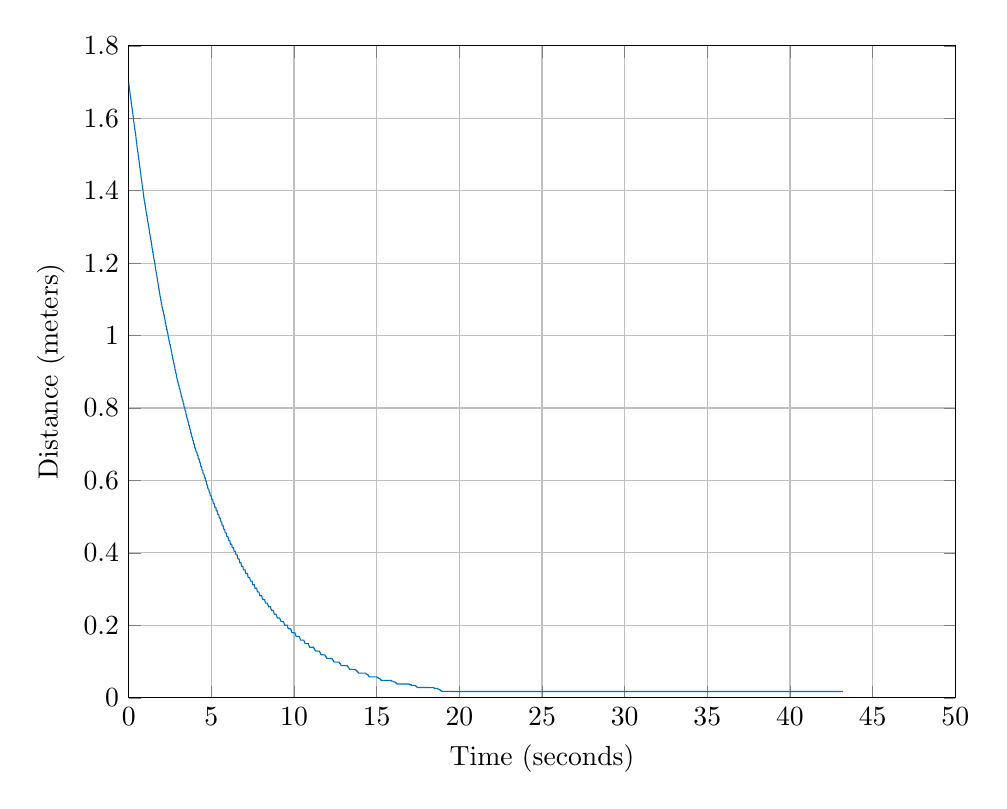
\begin{tikzpicture}

\begin{axis}[%
width=4.133in,
height=3.26in,
at={(0.693in,0.44in)},
scale only axis,
xmin=0,
xmax=50,
xmajorgrids,
xlabel={Time (seconds)},
ymin=0,
ymax=1.8,
ymajorgrids,
ylabel={Distance (meters)},
axis background/.style={fill=white}
]
\addplot [color=mycolor1,solid,forget plot]
  table[row sep=crcr]{%
0	1.70070137502122\\
0.0150263859999999	1.69086836645218\\
0.0310508189999983	1.68694825276524\\
0.047106237999998	1.67910941359981\\
0.0631314529999979	1.67518888235766\\
0.0792779730009995	1.66931010111042\\
0.0952288600009978	1.66343048690221\\
0.111220470999997	1.65951078862103\\
0.127221406000998	1.65167111649463\\
0.143358967	1.64971147613164\\
0.159183676999997	1.64027822955148\\
0.175062704999998	1.63791882719962\\
0.191183244999997	1.63007915507321\\
0.207090103000998	1.62811951471023\\
0.223258086999997	1.62027984258383\\
0.238996928999998	1.61635972889688\\
0.255097807	1.60852088973145\\
0.271256180999998	1.6065604164075\\
0.287224967999998	1.59872157724206\\
0.303064732000999	1.5912483885801\\
0.321278167999998	1.58692892831004\\
0.33637943	1.57908925618363\\
0.352108583999999	1.57712961582065\\
0.367110524000999	1.56928994369425\\
0.383221836999997	1.56733030333126\\
0.399035195999999	1.55949063120486\\
0.417372812999997	1.55753099084187\\
0.432501781000998	1.54969131871547\\
0.447765412000999	1.54417763057477\\
0.463008020999998	1.53593902942045\\
0.479174237	1.53201884599173\\
0.495857138	1.52613971693107\\
0.511271386	1.51830004480466\\
0.527037046999998	1.51634040444168\\
0.543367	1.50850073231528\\
0.559373543001	1.50654109195229\\
0.575063919000998	1.49870141982589\\
0.591195334999997	1.49554591464862\\
0.607062041000999	1.48690877089386\\
0.625229621999998	1.48298865720692\\
0.640427482000999	1.47710945840447\\
0.655604305999998	1.47318934471753\\
0.671171848999999	1.4653505055521\\
0.687137897000998	1.46143032212337\\
0.703052651	1.45555119306271\\
0.719111625	1.44967095171579\\
0.735188351	1.44455601575904\\
0.751021944001	1.43591887200428\\
0.767055976999998	1.43395923164129\\
0.784291217999998	1.42611955951489\\
0.799327373999998	1.42219944582795\\
0.815019684	1.4163202470255\\
0.833113220999997	1.41240013333856\\
0.848108011999998	1.40456129417313\\
0.863289062999997	1.40260082084917\\
0.879034967999998	1.39396177372338\\
0.895201538999997	1.39080817191715\\
0.911131890999999	1.38296933275171\\
0.927323467999998	1.3770897185435\\
0.944807386999998	1.37317002026233\\
0.959791704999998	1.37120954693837\\
0.975083079999998	1.36337070777294\\
0.991111937000997	1.36337070777294\\
1.00708324	1.35553103564653\\
1.023118533	1.35357139528355\\
1.039292129	1.34573172315715\\
1.055055816	1.3421785083404\\
1.071174807001	1.3378585629228\\
1.087251758001	1.33197943386213\\
1.103058108	1.33197943386213\\
1.119079553001	1.32413976173573\\
1.13518491	1.32218012137274\\
1.151158387	1.31434044924634\\
1.167240680001	1.31238080888336\\
1.183070422	1.30846062545463\\
1.199105916001	1.30258149639397\\
1.215540976	1.30062102307001\\
1.231048644	1.29394161630721\\
1.247183456001	1.29078884746194\\
1.263028664	1.28294917533554\\
1.279170359001	1.28098953497255\\
1.295116446	1.27510992076434\\
1.311032756	1.27119022248316\\
1.32918229	1.26922974915921\\
1.344242757999	1.26139090999378\\
1.35945863	1.26139090999378\\
1.375283085	1.25355123786737\\
1.391149468	1.25159159750439\\
1.407106514	1.24335113737866\\
1.423099078	1.23979894857236\\
1.439122092	1.23783847524841\\
1.455223893001	1.22999963608297\\
1.471083001	1.22999963608297\\
1.487189738	1.22215996395657\\
1.503062007	1.22020032359358\\
1.519046004	1.21236065146718\\
1.535005671	1.2104010111042\\
1.551694438	1.20648082767547\\
1.567040437	1.20060169861481\\
1.583170219	1.20060169861481\\
1.599008625	1.19156205653917\\
1.617208315	1.18880904968278\\
1.631048623001	1.18096937755638\\
1.64725563	1.17900973719339\\
1.663032329001	1.17508955376467\\
1.679286911	1.169210424704\\
1.695277676	1.16724995138005\\
1.711181968	1.1613707525776\\
1.727069255	1.15941111221461\\
1.743511887	1.15157144008821\\
1.759005161	1.14961179972523\\
1.777159165999	1.14293197755666\\
1.79222575	1.1378191507932\\
1.807236156001	1.13585867746924\\
1.823123088001	1.12801983830381\\
1.839090463	1.12801983830381\\
1.855236642001	1.12018016617741\\
1.871172187	1.11822052581442\\
1.88723717	1.11038085368802\\
1.903276282	1.10842121332503\\
1.919526874	1.10646074000108\\
1.934999975001	1.09862190083565\\
1.951057331001	1.09822111283632\\
1.967079179	1.09154168953949\\
1.983045839	1.08682925190362\\
2.001187592	1.08682925190362\\
2.016158013	1.07898957977722\\
2.031135198999	1.07702993941423\\
2.047214748001	1.07702993941423\\
2.063239502001	1.06919026728783\\
2.079079852001	1.06723062692484\\
2.095107581001	1.06723062692484\\
2.111122566	1.05939095479844\\
2.127119058001	1.05743131443545\\
2.143154251	1.05743131443545\\
2.159029455	1.04959164230905\\
2.175181225001	1.04723121394674\\
2.191239745	1.04487132066175\\
2.207050961	1.03819465023095\\
2.223175602001	1.03583935301404\\
2.239112462	1.03387887969008\\
2.255003308	1.02604004052465\\
2.271244408	1.02604004052465\\
2.287141037	1.02407956720069\\
2.302989091001	1.01624072803526\\
2.3190952	1.01624072803526\\
2.335105116001	1.01036048668835\\
2.351334552	1.00644141554587\\
2.367303743	1.00644141554587\\
2.38333648	0.998601743419472\\
2.399337316	0.996241315057155\\
2.415164362	0.995841895096126\\
2.431282092	0.987204751341372\\
2.447345755	0.984849454124458\\
2.463242214	0.984849454124458\\
2.479173892	0.977009781998056\\
2.495158140001	0.97505014163507\\
2.511243161	0.97505014163507\\
2.527164995	0.967210469508668\\
2.543110169001	0.965250829145682\\
2.559033782	0.963290355821726\\
2.577170217	0.95741115701928\\
2.592169825	0.955451516656293\\
2.607226327	0.953491043332338\\
2.623112286001	0.945652204166905\\
2.639030925001	0.944851996206546\\
2.655190359001	0.942094051254238\\
2.671242142001	0.933859555234878\\
2.687283575	0.933859555234878\\
2.703149304	0.929939371806154\\
2.719153301001	0.924060242745489\\
2.735132469	0.924060242745489\\
2.751159648	0.918180001398572\\
2.767278831001	0.914260930256101\\
2.783022803	0.914260930256101\\
2.799225548	0.906421258129699\\
2.815124923	0.904461617766713\\
2.830984357	0.904461617766713\\
2.84716266	0.896621945640311\\
2.863260384	0.894261517277994\\
2.879021354	0.893462335328085\\
2.895101336002	0.884829296708284\\
2.913498653	0.882869656345298\\
2.928817763	0.880909183021342\\
2.943248175001	0.875029984218896\\
2.959285913	0.873070343855909\\
2.975024146	0.873070343855909\\
2.993516631	0.869150439752469\\
3.008669429	0.863271031366521\\
3.023933058	0.863271031366521\\
3.039229297	0.863271031366521\\
3.055161075	0.855431359240119\\
3.071015549	0.853471718877132\\
3.087167807001	0.853471718877132\\
3.103130301	0.851511245553177\\
3.119006842	0.8452312587514\\
3.135133174	0.842872198427385\\
3.151243553	0.842472436438504\\
3.167125512	0.838154543370308\\
3.183158457	0.831879757455717\\
3.199196496001	0.831879757455717\\
3.215024224	0.831879757455717\\
3.231273903	0.824040085329315\\
3.247269817001	0.822080444966328\\
3.263252676999	0.822080444966328\\
3.279272029001	0.820119971642373\\
3.295292414001	0.81228113247694\\
3.311444817001	0.81228113247694\\
3.327144054	0.81228113247694\\
3.343264987001	0.804441460350538\\
3.359109407	0.802481819987552\\
3.375293568	0.802481819987552\\
3.391301044001	0.800521346663596\\
3.407263016	0.79424135986182\\
3.423299742	0.791482537548924\\
3.439265638	0.791482537548924\\
3.455007282	0.789124354585496\\
3.47112648	0.780889858566136\\
3.487139948999	0.780889858566136\\
3.503119774001	0.780889858566136\\
3.519468094	0.773050186439734\\
3.535147727001	0.771090546076748\\
3.551008081001	0.771090546076748\\
3.567127803	0.769130072752793\\
3.583166615	0.763250873950346\\
3.599079805001	0.76129123358736\\
3.615252646	0.76129123358736\\
3.631225939	0.753451561460958\\
3.647266229	0.751491921097971\\
3.663269605001	0.751491921097971\\
3.67912667	0.751091133098641\\
3.695045007999	0.74325146097224\\
3.711294441	0.740492638659344\\
3.727286071	0.740094929019871\\
3.743296573	0.738134455695916\\
3.759517467	0.729899959676556\\
3.775252565	0.729899959676556\\
3.791028824001	0.729899959676556\\
3.807131087	0.722060287550154\\
3.823132794	0.720100647187168\\
3.839117924	0.720100647187168\\
3.855101825	0.718140173863212\\
3.871266101	0.712260975060766\\
3.887291968	0.710301334697779\\
3.903387248	0.710301334697779\\
3.919360400001	0.706381151269056\\
3.936945400999	0.700502022208391\\
3.951926470001	0.700501739391416\\
3.967203435	0.700100951392086\\
3.982993344	0.698140598774125\\
3.999041397001	0.689502841157524\\
4.015047525	0.689502719339518\\
4.031097201001	0.689105820008804\\
4.047024487	0.689106311421269\\
4.065175758001	0.680871129933799\\
4.080185473999	0.678911350146945\\
4.095302203	0.678911714662618\\
4.111134266	0.678911878753197\\
4.127076934	0.676951129686427\\
4.143121277	0.671071252892338\\
4.15918745	0.669111529994949\\
4.175117045	0.669111529994949\\
4.191091438	0.669111535580515\\
4.207338333001	0.661270508673472\\
4.22312038	0.659310520198559\\
4.239065743	0.659310462565952\\
4.255064010001	0.659310451808755\\
4.271124523	0.657349496562009\\
4.28709946	0.651468787446514\\
4.303037278	0.649508468406313\\
4.319077749001	0.649508468406313\\
4.335056835	0.649110302470497\\
4.351022146	0.640871708464749\\
4.367065257999	0.638514408036162\\
4.383034705	0.638514408036162\\
4.399026136	0.638120556300227\\
4.41703265	0.636159323617516\\
4.432133784001	0.629885877812002\\
4.447088501	0.627925836233736\\
4.463010263001	0.627926349061798\\
4.478993566	0.627926349061798\\
4.495056714	0.620083869563768\\
4.511037576001	0.618123791998012\\
4.527060339	0.618123791998012\\
4.543032001	0.618123838217195\\
4.559009104	0.61616288540481\\
4.577120944001	0.610281052953472\\
4.592067969	0.608320563359116\\
4.607095557	0.608320728612819\\
4.623051290999	0.608320728612819\\
4.639032863	0.600477176560884\\
4.655042304	0.598516521307262\\
4.671036514	0.598516552015463\\
4.687058159001	0.598120823355269\\
4.703044351	0.596159228522221\\
4.719073550001	0.58948816970317\\
4.735075793001	0.587527489482518\\
4.751046825	0.587135969207011\\
4.767019631001	0.58713618822043\\
4.785070562	0.578902053064532\\
4.799948664001	0.576941617127854\\
4.815018499001	0.57694227141503\\
4.83308313	0.57694227141503\\
4.848029224	0.57498071785716\\
4.863168898	0.569098429002537\\
4.879012637	0.567137542422718\\
4.897071004	0.567137633624536\\
4.911561435	0.567138237297824\\
4.927020176001	0.559293119106854\\
4.944198081001	0.557332163860109\\
4.959312318	0.557332163860109\\
4.975075313001	0.557332163860109\\
4.991165611	0.557332163860109\\
5.007116557001	0.55537032137987\\
5.023119467	0.549487045669139\\
5.039188466	0.547526090422393\\
5.055037679	0.547526090422393\\
5.071017511999	0.54713180233335\\
5.087031948	0.54713180233335\\
5.103028899001	0.540461594957145\\
5.119074519	0.536539890643629\\
5.13511671	0.536539890643629\\
5.151053861	0.536149025306086\\
5.167094878001	0.536149025306086\\
5.184460840001	0.534187182825848\\
5.199583448	0.52791509600065\\
5.215175892001	0.525954140753904\\
5.231097633001	0.525954140753904\\
5.247298697	0.525954140753904\\
5.263198271	0.525954140753904\\
5.27910524	0.523992298273666\\
5.295124502	0.518109022562935\\
5.311240767001	0.516148067316189\\
5.327218609001	0.516148067316189\\
5.343122969	0.516148067316189\\
5.359203505	0.516148067316189\\
5.375157263001	0.508302949125219\\
5.391081222	0.506341993878473\\
5.407090284001	0.506341993878473\\
5.423083927	0.506341993878473\\
5.43926016	0.506341993878473\\
5.45511125	0.504380151398235\\
5.471129931001	0.498496875687504\\
5.487228719	0.496535920440758\\
5.503182898	0.496535920440758\\
5.519027707	0.496141632351716\\
5.535108510001	0.496141632351716\\
5.551010115	0.491432859218075\\
5.567467785001	0.48751067590874\\
5.583214114001	0.485549720661994\\
5.599194581001	0.485549720661994\\
5.61525881	0.485158855324451\\
5.631122847	0.485158855324451\\
5.64704204	0.476924926019015\\
5.663029553	0.474963970772269\\
5.679042848	0.474963970772269\\
5.695035706	0.474963970772269\\
5.71101451	0.474963970772269\\
5.729130966	0.473002128292031\\
5.744037226	0.467118852581299\\
5.759097929	0.465157897334553\\
5.777265124	0.465157897334553\\
5.792286336002	0.465157897334553\\
5.807128078	0.465157897334553\\
5.823007033	0.459273528210354\\
5.841119662	0.455351823896838\\
5.856031677	0.455351823896838\\
5.871026487	0.455351823896838\\
5.887041189	0.455351823896838\\
5.905093783	0.4533899814166\\
5.920015634	0.447506705705869\\
5.935012865	0.445545750459123\\
5.951093738	0.445545723119921\\
5.967182352	0.445151854809731\\
5.983003293	0.445151854809731\\
6.001073253001	0.445152162042437\\
6.015965154001	0.442797731148444\\
6.031023223	0.436522152402241\\
6.049107505	0.434561306344863\\
6.064963457	0.434561873409871\\
6.079900655	0.434561873409871\\
6.09501433	0.434172289312409\\
6.113091299001	0.434173192941059\\
6.128098185	0.43221111663825\\
6.14351308	0.426327213622934\\
6.159418019	0.423979265485838\\
6.175050569001	0.423979585320421\\
6.191062501	0.423979786690587\\
6.207059545	0.423980532958917\\
6.225185836	0.423980860691059\\
6.240702603	0.422018821392394\\
6.256256390001	0.416134881165037\\
6.2713205	0.414173715080313\\
6.287106042	0.414173715080313\\
6.303314311	0.414173863877595\\
6.319035036001	0.414174729617693\\
6.335106422	0.414174729617693\\
6.351064569	0.412212502921952\\
6.367039093	0.406328214713009\\
6.383020902	0.404366644152202\\
6.40108948	0.404366740615558\\
6.416288954	0.404367399051353\\
6.43121779	0.404367399051353\\
6.447006348	0.404367503531859\\
6.465111642001	0.402405443186543\\
6.479944078	0.396520082761432\\
6.495013053	0.394558420489804\\
6.511129527002	0.394558698979038\\
6.527005049	0.394168691933427\\
6.543047967	0.394168691933427\\
6.559075044	0.394169389463201\\
6.575515268	0.392206851524362\\
6.591089094	0.385543981381261\\
6.607067391	0.383582907003318\\
6.623044117001	0.383583405333431\\
6.639006185	0.383583405333431\\
6.655029685	0.383197676883373\\
6.673136384	0.383198983503459\\
6.688658652	0.38123612984239\\
6.703540491	0.375350074301874\\
6.719007779001	0.373005834785982\\
6.73501388	0.373005834785982\\
6.751045815001	0.37300612628996\\
6.767222005	0.373007148549757\\
6.783259479	0.373007571384433\\
6.79902766	0.37104488362779\\
6.81720738	0.365158983891453\\
6.83234433	0.363197167085106\\
6.847467035	0.363197407294635\\
6.863088438	0.363198276746654\\
6.87915726	0.363198649243047\\
6.895428696	0.363198649243047\\
6.911072642	0.361236381121564\\
6.929493771	0.355349634094867\\
6.944072385	0.353387318056507\\
6.95924012	0.353387590487828\\
6.975251987001	0.353387912885092\\
6.991241617001	0.353387912885092\\
7.007082397001	0.353387912885092\\
7.023188554	0.35338852436898\\
7.039138133001	0.35338852436898\\
7.055102183	0.349462282832218\\
7.072953399001	0.345538213335969\\
7.088192282001	0.343575897297608\\
7.103286733	0.343575897297608\\
7.119375407001	0.343576127897735\\
7.13517068	0.343188967427053\\
7.15131188	0.343188967427053\\
7.167113197	0.34318920641463\\
7.183182265001	0.343189495726751\\
7.199201946	0.339262854381212\\
7.215181799	0.334566327852165\\
7.23115411	0.332604243177555\\
7.24726297	0.332604243177555\\
7.263125299	0.332604432305206\\
7.279275284001	0.332604672116156\\
7.295239176001	0.332604672116156\\
7.311191882	0.332223054125403\\
7.327132354	0.330260123480859\\
7.343059103001	0.32633435173623\\
7.359349787	0.324372238292738\\
7.375210072	0.322410594980255\\
7.391221705	0.322031718580824\\
7.407218248	0.322031718580824\\
7.423206124001	0.322032209276323\\
7.4390977	0.322032751083291\\
7.455246391	0.322032751083291\\
7.471263644	0.320069398908688\\
7.487080595	0.316143912086715\\
7.50323901	0.312219482604863\\
7.519154672	0.312219924001816\\
7.535094086002	0.312220416868963\\
7.551198604	0.312220416868963\\
7.567217874	0.312220866844316\\
7.583190039	0.312221368289777\\
7.599228757	0.312221368289777\\
7.615122546	0.308294058388346\\
7.631235374	0.304369938308688\\
7.647142331	0.302407622270328\\
7.663256082	0.302407622270328\\
7.679198701001	0.302408476050806\\
7.695129661	0.302408476050806\\
7.711209988	0.302408476050806\\
7.727342428001	0.302409347107563\\
7.743067257999	0.302409347107563\\
7.759259907	0.298481249007489\\
7.77517206	0.294557036976736\\
7.791120096	0.292595125341545\\
7.807218202	0.292595125341545\\
7.823324359	0.292595486254993\\
7.839115601	0.292595899356071\\
7.855195596001	0.292208457960671\\
7.871146417	0.292208827572087\\
7.887175186	0.290244805806125\\
7.90309721	0.28828075648686\\
7.919103609001	0.283970090710673\\
7.937044246	0.281622045691217\\
7.952146421001	0.281622045691217\\
7.967517905	0.281622045691217\\
7.983210417	0.281622045691217\\
7.999246677	0.281622045691217\\
8.015124749	0.281622045691217\\
8.031319985	0.281622045691217\\
8.047245995	0.281244883161791\\
8.063065631	0.277316324420396\\
8.07923832	0.275353873617665\\
8.095157316	0.273391760174173\\
8.111166209	0.271429444135813\\
8.127336573	0.271429444135813\\
8.143260399001	0.271429444135813\\
8.159254800001	0.271429444135813\\
8.175179623001	0.271053995763618\\
8.193485888	0.271053995763618\\
8.208717345001	0.271053995763618\\
8.224222481	0.271053995763618\\
8.239325883001	0.267125437022224\\
8.255020934	0.265162986219492\\
8.271171835	0.263200872776\\
8.289324312001	0.26123855673764\\
8.304566934	0.26123855673764\\
8.319730657001	0.26123855673764\\
8.335313791001	0.26123855673764\\
8.351116517	0.26123855673764\\
8.367205026	0.26123855673764\\
8.383135682001	0.26123855673764\\
8.399171331001	0.26123855673764\\
8.415199744	0.257309997996245\\
8.431113103	0.255347547193513\\
8.447284653	0.253385433750022\\
8.463240757	0.251423117711661\\
8.479137983	0.251423117711661\\
8.495086712	0.251423117711661\\
8.511184094	0.251423117711661\\
8.527234031	0.251423117711661\\
8.543094532	0.251423117711661\\
8.559495665	0.251423117711661\\
8.575248933	0.251423117711661\\
8.59130806	0.247494558970267\\
8.607205755	0.245532108167535\\
8.623172926999	0.243569994724044\\
8.639240856	0.241607678685683\\
8.655262698	0.241607678685683\\
8.671231801	0.241607678685683\\
8.687163788	0.241607678685683\\
8.703387611	0.241607678685683\\
8.719165220001	0.241220237290283\\
8.735071257	0.241220237290283\\
8.751126925001	0.239255793725348\\
8.767028690001	0.237291678548889\\
8.783205591	0.235329227746157\\
8.799198959001	0.231404798264305\\
8.815208474	0.231018384282164\\
8.831049221	0.230632655301068\\
8.847208986	0.230632655301068\\
8.863289317001	0.230632655301068\\
8.879276687001	0.230632655301068\\
8.895454643	0.230632655301068\\
8.91106899	0.230632655301068\\
8.927120079001	0.228668211736132\\
8.944888819001	0.226704096559673\\
8.960111395	0.224741645756942\\
8.975315084	0.222402369784024\\
8.993743166001	0.220440053745664\\
9.009010814	0.220440053745664\\
9.024154888	0.220440053745664\\
9.039885939	0.220440053745664\\
9.055246513	0.220440053745664\\
9.071229254001	0.220440053745664\\
9.087130945	0.220440053745664\\
9.103158924001	0.220440053745664\\
9.119049098	0.220440053745664\\
9.135266423001	0.220064605373469\\
9.151191547	0.218100161808534\\
9.167213340001	0.216136046632075\\
9.183268262	0.214173595829343\\
9.199098473001	0.212211482385851\\
9.215113323999	0.210249166347491\\
9.231100809	0.210249166347491\\
9.247005727001	0.210249166347491\\
9.263232606	0.210249166347491\\
9.279078282	0.210249166347491\\
9.295047951001	0.210249166347491\\
9.311271707	0.210249166347491\\
9.327027302	0.210249166347491\\
9.345129329001	0.210249166347491\\
9.359960794	0.210249166347491\\
9.375015314	0.208284722782555\\
9.391045261	0.206320607606096\\
9.407014474	0.204358156803364\\
9.423069021	0.202396043359873\\
9.439067057001	0.200433727321512\\
9.455069411	0.200433727321512\\
9.471185361	0.200433727321512\\
9.486999211	0.200433727321512\\
9.505002575	0.200433727321512\\
9.519887785	0.200433727321512\\
9.535066654001	0.200433727321512\\
9.551010441	0.200433727321512\\
9.569222723001	0.200433727321512\\
9.584573198999	0.200433727321512\\
9.600521817001	0.198469283756577\\
9.615720849	0.196505168580118\\
9.631228813	0.192580604333895\\
9.648056605	0.192580604333895\\
9.663421943	0.190618288295534\\
9.67909028	0.190618288295534\\
9.695291934	0.190618288295534\\
9.711247367	0.190618288295534\\
9.727163295	0.190618288295534\\
9.743193571	0.190618288295534\\
9.759197683	0.190618288295534\\
9.775797266001	0.190618288295534\\
9.791142446	0.190230846900134\\
9.808725547	0.190230846900134\\
9.823879694	0.18630228815874\\
9.839111690001	0.18630228815874\\
9.85511679	0.182377723912516\\
9.871198239	0.180415407874156\\
9.887041948	0.180415407874156\\
9.903011471	0.180028993892015\\
9.921144942001	0.179643264910919\\
9.936070600001	0.179643660659369\\
9.951240131	0.179644070596962\\
9.967121664001	0.179644965600236\\
9.983172342	0.179645719581006\\
9.999209495	0.179646138909631\\
10.0152292	0.179647052694864\\
10.031302517001	0.179647410927241\\
10.047211025	0.1796482541533\\
10.063180499	0.177684546840511\\
10.079205403	0.175720602062872\\
10.095064426001	0.173758746239316\\
10.111064676999	0.171796362788881\\
10.127105102	0.169834973069372\\
10.143094538	0.169835341074901\\
10.161440788	0.169459929997691\\
10.176687448999	0.169461429568089\\
10.191884268	0.169461807012405\\
10.207230874	0.169462196612511\\
10.223117065	0.169463724534606\\
10.239243149001	0.169464111417698\\
10.255349112	0.169464510468552\\
10.271263913	0.169465384175974\\
10.287195567001	0.169466463064154\\
10.303380359001	0.169466871565743\\
10.319089543001	0.169467764174532\\
10.337241709	0.167503831057619\\
10.352548351	0.165539609129977\\
10.367845782	0.163205104187496\\
10.383504121	0.16124302072152\\
10.399245815	0.159281153684379\\
10.415157585	0.159281153684379\\
10.431220458001	0.159282596125578\\
10.447015422	0.159283668703708\\
10.465339994002	0.159283668703708\\
10.48048495	0.159285139675809\\
10.495629539001	0.159285851903708\\
10.511329466	0.159286231274313\\
10.52737979	0.159287730777272\\
10.543493997	0.159288452515048\\
10.559173326001	0.159288841396117\\
10.575217988	0.159290369429888\\
10.591217546	0.159291100677519\\
10.607133328	0.157326143975934\\
10.623191418001	0.155362050967636\\
10.639205949001	0.15339995828655\\
10.654996813	0.15143724515103\\
10.671205615	0.14947474964092\\
10.687150862	0.149475377889471\\
10.703081687001	0.149476414274187\\
10.719173262	0.149477192271338\\
10.735164600001	0.149477830089669\\
10.751179533	0.149478885614261\\
10.767266589	0.149478885614261\\
10.78322712	0.149480330139847\\
10.799118134	0.14948103494608\\
10.815232996	0.149481404804283\\
10.833569071	0.149482878039928\\
10.848618545	0.149483592415778\\
10.863806739001	0.149483971844176\\
10.879104206001	0.147519795994408\\
10.895484343	0.145555100485908\\
10.911210307001	0.143591770348582\\
10.927273013	0.141629104838158\\
10.945027478001	0.139666732569492\\
10.960217936	0.139667064742667\\
10.975414233	0.139667806128651\\
10.991042257	0.139668427195248\\
11.009177456	0.139669447841887\\
11.024308276	0.139670208487726\\
11.039469501	0.139670839183855\\
11.055185611	0.139671879089867\\
11.071216661001	0.139671879089867\\
11.087048934	0.13967329932118\\
11.103240717	0.139674358486533\\
11.119170266	0.139674358486533\\
11.135100862	0.139675807607147\\
11.151078326001	0.139676515338811\\
11.167236004001	0.139676886031809\\
11.183192359001	0.13967836404168\\
11.199232524001	0.137334077939515\\
11.215163501	0.135369058857136\\
11.231091569	0.135370501455262\\
11.247158676	0.13340698353014\\
11.263131082	0.13144379882008\\
11.279187503001	0.131444590027307\\
11.295287506001	0.129481762191162\\
11.311216145001	0.129482438571071\\
11.32751603	0.129483183300476\\
11.343253963	0.129484490019262\\
11.359363134	0.1294851761004\\
11.375179225001	0.129109463308228\\
11.393494416001	0.129110097289216\\
11.407209935	0.129111485187793\\
11.423078912001	0.128735693961237\\
11.439245805001	0.128737806805382\\
11.455260872	0.128738508610749\\
11.471083589	0.12873921409428\\
11.487183468	0.128741356029861\\
11.503109782001	0.128742067524342\\
11.519138343	0.128742782709038\\
11.536448842	0.128744953735989\\
11.551681661001	0.126779101522187\\
11.567198505	0.124813635402643\\
11.583188716	0.124815162782999\\
11.599084488	0.122851799109502\\
11.61507002	0.12088815568955\\
11.631288176	0.118925062651859\\
11.64709879	0.118925681257086\\
11.663128772001	0.11892703708638\\
11.679175942001	0.118928472633511\\
11.695228834999	0.118929787835984\\
11.711192537	0.118930476326938\\
11.727302776	0.118931213622154\\
11.743214815001	0.118932569499046\\
11.759258161001	0.118933964348\\
11.775151974	0.118569150081858\\
11.791178867	0.118571615739756\\
11.807288113	0.118572322085754\\
11.823143734001	0.118573030098477\\
11.839012632999	0.118575525038045\\
11.855187561	0.118576241132914\\
11.87112481	0.11857695890649\\
11.887146676001	0.116612529494875\\
11.903263187	0.114646555256007\\
11.91913674	0.114647282790414\\
11.937167473001	0.112684676977047\\
11.952369415	0.112685349466641\\
11.967522077	0.110721251105503\\
11.98347752	0.108757707988175\\
11.999152525	0.108758674693346\\
12.015160638	0.108760038908568\\
12.031214249001	0.108760750287262\\
12.047311733	0.108762457832097\\
12.063178587	0.108763841676642\\
12.079186937	0.108763841676642\\
12.095237635001	0.108405595107298\\
12.111387583001	0.1084066403707\\
12.127363645	0.108407341928819\\
12.143218617	0.10840981977411\\
12.159228859001	0.108410874857152\\
12.175266362001	0.108411586235846\\
12.191213812001	0.108414093541906\\
12.207083587	0.108415158444554\\
12.223270577	0.108415879643802\\
12.239171781001	0.108417400606257\\
12.255153353	0.108419491132777\\
12.27110628	0.108420222152556\\
12.28707795	0.108421762755892\\
12.30313303	0.108422788379922\\
12.32084195	0.106457093820611\\
12.336084738	0.104491511123155\\
12.351448056	0.10449248358378\\
12.367574979	0.104494265982297\\
12.383211542	0.102528652607586\\
12.399216015001	0.100565795318942\\
12.415154439	0.098601983863007\\
12.431277427	0.098601983863007\\
12.447195359001	0.098604446767059\\
12.46349878	0.0986054982635909\\
12.479152849	0.0986062039649329\\
12.495192247	0.0986086965089661\\
12.511208417	0.0986097578848453\\
12.527247724	0.0986104734664766\\
12.543188479	0.0986129956504149\\
12.559473137	0.0986140669056095\\
12.575154012	0.0986147923675083\\
12.591237079001	0.0986163223329763\\
12.607122641	0.0986184253257523\\
12.623192085	0.0986191606678968\\
12.63917349	0.0986207103936723\\
12.655186418001	0.0986217421314133\\
12.671216089001	0.0986235783675076\\
12.687117129	0.0986243532304072\\
12.703204854	0.0986261894706966\\
12.719149673001	0.0986280454662074\\
12.735220081001	0.0986280454662074\\
12.751166287001	0.0966626669576867\\
12.767197667	0.0946960079536725\\
12.783337046	0.0946967729364179\\
12.799156077	0.0946993808749932\\
12.815224759	0.0927342484368447\\
12.831288847	0.090769088420253\\
12.847126674	0.0888055351127111\\
12.863222508001	0.0888066036190143\\
12.879185718	0.0888073242407375\\
12.895152484	0.0888098638144914\\
12.911138795	0.08881094225983\\
12.927281456001	0.0888116728215478\\
12.944841324001	0.0888124332031139\\
12.959993382999	0.088813521587455\\
12.975205219	0.088813521587455\\
12.991279801001	0.088813521587455\\
13.007221637	0.0888146199107651\\
13.023104491001	0.0888146199107651\\
13.039111441	0.0888146199107651\\
13.05512152	0.0888146199107651\\
13.071207544	0.0888157281730111\\
13.087252925001	0.0888157281730111\\
13.103095386	0.0888157281730111\\
13.119167167	0.0888168463741597\\
13.135253025	0.0888168463741597\\
13.151134340001	0.0888168463741597\\
13.167228303	0.0888179745141757\\
13.183224284001	0.0888179745141757\\
13.199080755	0.0888179745141757\\
13.215170776	0.0888191125930256\\
13.231223434	0.0868504745998502\\
13.247110029	0.0868504745998502\\
13.263239928001	0.08488366628963\\
13.279230364001	0.08488366628963\\
13.295336612001	0.08488366628963\\
13.312811484001	0.0829173475806542\\
13.327949608	0.0809523809904267\\
13.343215143	0.0809523809904267\\
13.361645615	0.0789861261032996\\
13.37682541	0.0786203592506389\\
13.391930801	0.0786203592506389\\
13.407237232	0.0786203592506389\\
13.423140649001	0.0786214757199957\\
13.439049646	0.0786214757199957\\
13.455242559	0.0786214757199957\\
13.471088367	0.0786226021879859\\
13.487234307001	0.0786226021879859\\
13.503243557001	0.0786226021879859\\
13.519071100001	0.0786237386545743\\
13.535230054	0.0786237386545743\\
13.551240954	0.0786237386545743\\
13.567221790999	0.0786248851197267\\
13.583205320001	0.0786248851197267\\
13.599213329001	0.0786248851197267\\
13.615148556	0.0786248851197267\\
13.631207733	0.0786260415834081\\
13.647218673001	0.0782601977385127\\
13.663171573	0.0782601977385127\\
13.679203579	0.0782613642006882\\
13.695166768	0.0782613642006882\\
13.711178154001	0.0782613642006882\\
13.727270826001	0.0782625406613215\\
13.743180976	0.0759277892599783\\
13.759393756	0.0759277892599783\\
13.775101223001	0.0759289147744251\\
13.791190172	0.0739610199909495\\
13.807182678	0.0739610199909495\\
13.8231929	0.0739621555637715\\
13.839195221	0.0719958368547959\\
13.855060118	0.0719958368547959\\
13.87116437	0.0700309194237412\\
13.887231321	0.0700309194237412\\
13.903218703	0.0680646645366139\\
13.919076341	0.0680658202260815\\
13.936522596	0.0680658202260815\\
13.951867588001	0.0680677203785161\\
13.967276515001	0.0680686760254714\\
13.98318682	0.0680698417732095\\
13.999263417	0.0680727479150423\\
14.015197486	0.0680737136328953\\
14.031210624	0.0680748894388681\\
14.047164152002	0.0680769014411335\\
14.063180573999	0.0680778257812882\\
14.07916377	0.0680799874341815\\
14.095131507	0.0680810135767942\\
14.111232429	0.0680829539770993\\
14.12738718	0.0680851357589947\\
14.143171835	0.0680861719722934\\
14.159442107	0.0680881325023199\\
14.175138907	0.0680903344131507\\
14.191183271	0.0680913806971031\\
14.207331095001	0.0680933613567922\\
14.223201570001	0.0680955833964907\\
14.239124435	0.0680966397510654\\
14.255208301	0.0680986405403565\\
14.271237180001	0.0680996566122523\\
14.287209072	0.0681008827088556\\
14.30318159	0.0681039700528521\\
14.319185323	0.0681049961954647\\
14.335129718	0.0681062323500832\\
14.351124921	0.066138387086492\\
14.367244006001	0.0661393717802286\\
14.383213997	0.0661415939814995\\
14.399112204	0.0661437469729114\\
14.415155596	0.0641762270009893\\
14.431313202	0.0641784693908649\\
14.447193468	0.0641806425233258\\
14.46323456	0.0641815856703583\\
14.47911851	0.0618636926682175\\
14.495260048001	0.0618647362724636\\
14.511265184	0.0599003559065727\\
14.527185462	0.0599025753308382\\
14.543221982	0.0579366754326525\\
14.559303091	0.0579390158885094\\
14.57515779	0.0579412555610854\\
14.591245001	0.0579412555610854\\
14.607184948	0.0579446801416341\\
14.623167757	0.057945703485095\\
14.639247461002	0.0579469400624528\\
14.655220323	0.0579503950329974\\
14.671175876	0.0579514285068667\\
14.687177909001	0.0579526752019897\\
14.703269134	0.0579548231923279\\
14.719147977001	0.0579561605624259\\
14.735348610001	0.0579584609795223\\
14.751198520001	0.0579606292303558\\
14.767234715001	0.057961976729743\\
14.783215342	0.0579642973948735\\
14.799182809	0.0579654017807032\\
14.815112832	0.0579678435347715\\
14.831155599	0.0579701844478659\\
14.847278852	0.0579712989638437\\
14.863117698	0.0579737609773339\\
14.879190724	0.0579761221383204\\
14.895333566	0.0579772467844122\\
14.911195662	0.0579797290572486\\
14.92769654	0.0579821104660552\\
14.943153903	0.0579821104660552\\
14.959461205	0.0579857477743344\\
14.975178525001	0.0579868420299827\\
14.991215965	0.0579881494308889\\
15.007211974	0.0579904189831977\\
15.023158416001	0.0560210607757816\\
15.039203662	0.0560234232356702\\
15.055212841001	0.0560257130480688\\
15.071264713	0.0560271213223178\\
15.087174982001	0.0560295040898413\\
15.10315482	0.0540613575731992\\
15.119086378	0.0540638599980392\\
15.135256387	0.0537265320400113\\
15.151253093	0.0537277073361533\\
15.167239596	0.0537302300799463\\
15.183130628001	0.0537329974606591\\
15.199300841001	0.0517662258393425\\
15.215205353	0.0517687689020117\\
15.233558600001	0.0498038489683292\\
15.248738941	0.0498049823203035\\
15.264008118	0.0498075457017713\\
15.279306277	0.0478407435108048\\
15.295321946	0.047842396490714\\
15.311194073	0.0478460614687697\\
15.32713617	0.0478471642511957\\
15.343091205	0.0478488274187132\\
15.361746398	0.0478511145021876\\
15.376911905	0.0478536359374138\\
15.392220358	0.0478553092924887\\
15.407496875	0.0478576167554543\\
15.423200902	0.047859035407102\\
15.43916332	0.0478618421118422\\
15.455212871001	0.0478630162227285\\
15.471236214	0.0478655987945646\\
15.487177033	0.0478684258765756\\
15.503090600001	0.0478696101771017\\
15.519011353	0.0478722131272926\\
15.535267106	0.0478750605864884\\
15.551166076	0.0478762550766172\\
15.567383642001	0.0478788784050845\\
15.583121733	0.0478817462413774\\
15.599225696	0.0478817462413774\\
15.615173952001	0.0478855946277363\\
15.631239584	0.0478867585489473\\
15.647165489001	0.04788848284104\\
15.663207079001	0.0478908922003956\\
15.679216101	0.0478923617950442\\
15.695034216	0.0478952703852702\\
15.711199064	0.047897700123686\\
15.727313081001	0.0478991799068023\\
15.743174906001	0.0479021088738623\\
15.761632209	0.0479033441220376\\
15.776832600001	0.047906048962802\\
15.792066943	0.0479089983066068\\
15.807640345	0.0479102437442005\\
15.823274613	0.047912968962835\\
15.839178008001	0.0479159386832939\\
15.855178142001	0.0479171943102683\\
15.871130167	0.0479199399066899\\
15.887254277	0.0479229300037132\\
15.903234726	0.0459511128397039\\
15.919102671	0.0459551446301454\\
15.935057287	0.0459568716814776\\
15.951086866001	0.0459568716814776\\
15.967218547	0.0459584024062476\\
15.98322864	0.0459584024062476\\
15.999148455	0.0439897412786112\\
16.015290326	0.0439897412786112\\
16.031370883001	0.0439912223870638\\
16.047187669999	0.0439929699323276\\
16.063269927	0.0439929699323276\\
16.079213585	0.0439944612889489\\
16.095272086	0.043996219081099\\
16.111087697	0.043996219081099\\
16.1271044	0.0420288982393997\\
16.143156860001	0.0420306662783825\\
16.159154943	0.0420306662783825\\
16.175184900001	0.0400636634067189\\
16.191333260001	0.0400654416924804\\
16.207155672	0.0400654416924804\\
16.223098604	0.0380982642557655\\
16.239182727	0.0381000527882511\\
16.255261862	0.0381000527882511\\
16.272577658	0.0381015851370901\\
16.287782093	0.0381015851370901\\
16.303211563	0.0381033839162461\\
16.319114937	0.0381033839162461\\
16.33647821	0.0381049265130233\\
16.351688053	0.0381067355387947\\
16.367256263001	0.0381067355387947\\
16.383476896	0.0381082883834636\\
16.399222508001	0.038110107655795\\
16.414990082	0.038110107655795\\
16.431212141	0.038111670748308\\
16.447137595001	0.0381135002671442\\
16.463136581001	0.0381135002671442\\
16.479215083001	0.038115073607454\\
16.495341988	0.0381169133727393\\
16.511224461002	0.0381169133727393\\
16.527318328	0.0381184969607975\\
16.543180346	0.0381203469724756\\
16.559356779001	0.0381203469724756\\
16.575152455	0.0381219408082343\\
16.591288815	0.0381219408082343\\
16.607164111	0.0381238010662492\\
16.623005213	0.0381254051496596\\
16.640843072	0.0381254051496596\\
16.655911317001	0.0381272756539544\\
16.671203219	0.0381272756539544\\
16.687203100001	0.0381288899849681\\
16.70321263	0.0381307707354859\\
16.719243874	0.0381307707354859\\
16.73526016	0.0381323953140533\\
16.751093056001	0.038134286310737\\
16.767169606	0.038134286310737\\
16.783115149001	0.0381359211368089\\
16.799497402	0.0381378223796001\\
16.815236102001	0.0381378223796001\\
16.831019908	0.0381394674531264\\
16.849251537	0.038141378941968\\
16.864543821	0.038141378941968\\
16.879739181	0.0381430342628988\\
16.895034155	0.0381449559977325\\
16.911167271	0.0381449559977325\\
16.927271516	0.0381466215660171\\
16.944942822	0.0381466215660171\\
16.960151157001	0.0381485535467845\\
16.975229050001	0.0361771991823989\\
16.991224305	0.0361771991823989\\
17.007258477	0.0361790843073684\\
17.023147997	0.0361790843073684\\
17.039044549001	0.0361807703702086\\
17.055236502	0.0361826658010975\\
17.071153708001	0.0361826658010975\\
17.087197688	0.0361843621111382\\
17.103300409001	0.0342145675909613\\
17.119086028	0.0342145675909613\\
17.135114569	0.0342162156645787\\
17.151194915	0.0342181317071322\\
17.167170318	0.0342181317071322\\
17.183166220001	0.03421979008791\\
17.19932077	0.0342217164362082\\
17.215290004001	0.0342217164362082\\
17.231179031001	0.0342233851240958\\
17.247224813	0.0342233851240958\\
17.263138509	0.0342253217780804\\
17.279149619	0.0342270007730274\\
17.29528954	0.0342270007730274\\
17.311160159001	0.0342289477326392\\
17.327187244002	0.0342289477326392\\
17.343225701001	0.0322618145881495\\
17.359360024001	0.0322637718533292\\
17.375184673001	0.0322637718533292\\
17.391268282001	0.0322654714622406\\
17.407130994002	0.0302989243084428\\
17.423369007	0.0302989243084428\\
17.439103588001	0.0303006342242584\\
17.455185037	0.0283339125628261\\
17.471254046	0.0283339125628261\\
17.48718787	0.0283356327854944\\
17.503066974	0.028337620967019\\
17.519074212	0.028337620967019\\
17.535208277	0.0283393514964874\\
17.551171752	0.0283413499833396\\
17.567225334	0.0283413499833396\\
17.583175533	0.0283430908195559\\
17.599076798001	0.0283430908195559\\
17.615171145001	0.0283450996116743\\
17.631194854	0.0283468507545848\\
17.647310242	0.0283468507545848\\
17.663195841	0.0283488698519092\\
17.679226043001	0.0283488698519092\\
17.695271454	0.0283506313014608\\
17.711167527002	0.0283526607039291\\
17.727291812001	0.0283526607039291\\
17.743172866	0.028354432460068\\
17.75924375	0.0283564721676184\\
17.775148427	0.0283564721676184\\
17.791232434	0.0283582542302909\\
17.807177671	0.0283603042428613\\
17.823227441	0.0283603042428613\\
17.839200489001	0.0283620966120131\\
17.855202531001	0.0283641569295412\\
17.871337741	0.0283641569295412\\
17.887069336	0.0283659596051171\\
17.905310384	0.0283659596051171\\
17.920450744002	0.0283680302275402\\
17.935250407	0.0283698432094861\\
17.9511864	0.0283698432094861\\
17.967311247	0.0283719241367406\\
17.983273985999	0.0283719241367406\\
17.999221139	0.0283719241367406\\
18.015203377	0.0283740153687637\\
18.031220998001	0.0283740153687637\\
18.04719908	0.0283740153687637\\
18.063231827	0.0283761169054915\\
18.079158326001	0.0283761169054915\\
18.095171107001	0.0283761169054915\\
18.111198137	0.0283782287468599\\
18.127180761001	0.0283782287468599\\
18.143157957	0.0283782287468599\\
18.159520787	0.0283803508928044\\
18.175111588001	0.0283803508928044\\
18.191173871	0.0283803508928044\\
18.207256734001	0.0280290009823387\\
18.22318083	0.0280290009823387\\
18.23920141	0.0280290009823387\\
18.255180289	0.0280290009823387\\
18.271118246001	0.0280311437372418\\
18.28720138	0.0280311437372418\\
18.304729102	0.0280311437372418\\
18.319989664001	0.0280332967965264\\
18.335264749001	0.0280332967965264\\
18.351171171	0.0280332967965264\\
18.367465401	0.0280354601601267\\
18.383160233001	0.0280354601601267\\
18.399196749001	0.0280354601601267\\
18.415185090001	0.0280376338279769\\
18.431239362	0.0280376338279769\\
18.447202132	0.0280376338279769\\
18.463168743	0.0280398178000112\\
18.47919387	0.026065100721981\\
18.495210934	0.026065100721981\\
18.511240096	0.026067239700319\\
18.527327113	0.026067239700319\\
18.543168971	0.026067239700319\\
18.559572497	0.026067239700319\\
18.575381517001	0.0260693890428623\\
18.591309289	0.0260693890428623\\
18.607237616001	0.0260693890428623\\
18.623161264	0.0260715487495455\\
18.639238224	0.0260715487495455\\
18.655172062001	0.0260715487495455\\
18.67116684	0.0260737188203026\\
18.687163025999	0.0260737188203026\\
18.703154061	0.0241010325124409\\
18.719806559	0.0241032129472063\\
18.735107735	0.0241032129472063\\
18.751198472	0.0241032129472063\\
18.767121591	0.0241054037459132\\
18.783166742	0.0221365812994694\\
18.799150703	0.0221365812994694\\
18.816162571	0.0221387824620509\\
18.831224516	0.0221387824620509\\
18.847045503001	0.0201702677375653\\
18.865210175	0.0201724792639548\\
18.879061355001	0.0201724792639548\\
18.895056840001	0.0201724792639548\\
18.911022484001	0.0182037797263863\\
18.929224998001	0.0182060016165162\\
18.943807747	0.0182060016165162\\
18.959245781	0.0182060016165162\\
18.975010127	0.0182060016165162\\
18.9910307	0.0182060016165162\\
19.007013632	0.0178535500159009\\
19.025122849	0.0178535500159009\\
19.040253389	0.0178535500159009\\
19.055233281	0.0178535500159009\\
19.070995269	0.0178535500159009\\
19.087008206001	0.0178535500159009\\
19.103057053001	0.0178535500159009\\
19.119096106	0.0178535500159009\\
19.135364390001	0.0178535500159009\\
19.15101105	0.0178535500159009\\
19.167208038	0.0178535500159009\\
19.183190695001	0.0178535500159009\\
19.200001129001	0.0178535500159009\\
19.215291829	0.0178535500159009\\
19.231414449001	0.0178535500159009\\
19.247365415999	0.0178535500159009\\
19.263219093	0.0178535500159009\\
19.279183216001	0.0178535500159009\\
19.295290195	0.0178535500159009\\
19.311164760001	0.0178535500159009\\
19.327249522001	0.0178535500159009\\
19.343171797	0.0178535500159009\\
19.359395783	0.0178535500159009\\
19.375180159001	0.0178535500159009\\
19.391280770001	0.0178535500159009\\
19.407263499999	0.0178535500159009\\
19.423146031001	0.0175017856425228\\
19.439160963001	0.0175017856425228\\
19.45519792	0.0175017856425228\\
19.471192531	0.0175017856425228\\
19.48720563	0.0175017856425228\\
19.503090364001	0.0175017856425228\\
19.519144643	0.0175017856425228\\
19.535338646	0.0175017856425228\\
19.551114521	0.0175017856425228\\
19.567277782001	0.0175017856425228\\
19.583204494002	0.0175017856425228\\
19.599230524001	0.0175017856425228\\
19.615183361	0.0175017856425228\\
19.631211624	0.0175017856425228\\
19.647169061	0.0175017856425228\\
19.663225249	0.0175017856425228\\
19.679146699001	0.0175017856425228\\
19.695208529	0.0175017856425228\\
19.711227662001	0.0175017856425228\\
19.727133718	0.0175017856425228\\
19.743172681	0.0175017856425228\\
19.759466919	0.0175017856425228\\
19.775432876	0.0175017856425228\\
19.791318885001	0.0175017856425228\\
19.809505853	0.0175017856425228\\
19.824616363	0.0175017856425228\\
19.840002024001	0.0175017856425228\\
19.855285158	0.0175017856425228\\
19.871258057001	0.0175017856425228\\
19.887186576001	0.0175017856425228\\
19.903285569001	0.0175017856425228\\
19.919149489001	0.0175017856425228\\
19.937622252	0.0175017856425228\\
19.952910837	0.0175017856425228\\
19.968536227001	0.0175017856425228\\
19.983722485999	0.0175017856425228\\
19.999119683	0.0175017856425228\\
20.015049998001	0.0175017856425228\\
20.031241331	0.0175017856425228\\
20.047186655	0.0175017856425228\\
20.063162304	0.0175017856425228\\
20.079045545	0.0175017856425228\\
20.097353186	0.0175017856425228\\
20.112625871001	0.0175017856425228\\
20.1278167	0.0175017856425228\\
20.143176600001	0.0175017856425228\\
20.159273966001	0.0175017856425228\\
20.175046457	0.0175017856425228\\
20.19139816	0.0175017856425228\\
20.207004077	0.0175017856425228\\
20.223179992001	0.0175017856425228\\
20.239259301	0.0175017856425228\\
20.255541395	0.0175017856425228\\
20.271025009	0.0175017856425228\\
20.287265074001	0.0175017856425228\\
20.304245101	0.0175017856425228\\
20.319377985	0.0175017856425228\\
20.335264242	0.0175017856425228\\
20.351188153	0.0175017856425228\\
20.367162409001	0.0175017856425228\\
20.383190824001	0.0175017856425228\\
20.399260761999	0.0175017856425228\\
20.415282505	0.0175017856425228\\
20.431228712	0.0175017856425228\\
20.447189326001	0.0175017856425228\\
20.463196340001	0.0175017856425228\\
20.479230717	0.0175017856425228\\
20.495280748	0.0175017856425228\\
20.511232522001	0.0175017856425228\\
20.527167142001	0.0175017856425228\\
20.543189056	0.0175017856425228\\
20.561574285	0.0175017856425228\\
20.576793720001	0.0175017856425228\\
20.592200423	0.0175017856425228\\
20.60759737	0.0175017856425228\\
20.623184327	0.0175017856425228\\
20.639146831	0.0175017856425228\\
20.655216947	0.0175017856425228\\
20.671226468	0.0175017856425228\\
20.687240022001	0.0175017856425228\\
20.703221774001	0.0175017856425228\\
20.719131369002	0.0175017856425228\\
20.735452362	0.0175017856425228\\
20.751168423	0.0175017856425228\\
20.767229503001	0.0175017856425228\\
20.783159171001	0.0175017856425228\\
20.799203548001	0.0175017856425228\\
20.815015184	0.0175017856425228\\
20.831226527	0.0175017856425228\\
20.847202496001	0.0175017856425228\\
20.863238531001	0.0175017856425228\\
20.879174304	0.0175017856425228\\
20.895168171	0.0175017856425228\\
20.911135071	0.0175017856425228\\
20.927304113	0.0175017856425228\\
20.944925932001	0.0175017856425228\\
20.960226069001	0.0175017856425228\\
20.975442246001	0.0175017856425228\\
20.991309328	0.0175017856425228\\
21.007214286001	0.0175017856425228\\
21.023170891	0.0175017856425228\\
21.039123776	0.0175017856425228\\
21.055217439	0.0175017856425228\\
21.071156550001	0.0175017856425228\\
21.087054207	0.0175017856425228\\
21.10304541	0.0175017856425228\\
21.119182348	0.0175017856425228\\
21.13524391	0.0175017856425228\\
21.151168876	0.0175017856425228\\
21.167203575	0.0175017856425228\\
21.183179494002	0.0175017856425228\\
21.199214974	0.0175017856425228\\
21.215147579	0.0175017856425228\\
21.231240698999	0.0175017856425228\\
21.247169736	0.0175017856425228\\
21.265571588001	0.0175017856425228\\
21.280583284001	0.0175017856425228\\
21.295736601	0.0175017856425228\\
21.311198219	0.0175017856425228\\
21.327251654001	0.0175017856425228\\
21.343170373	0.0175017856425228\\
21.359247221	0.0175017856425228\\
21.375151507	0.0175017856425228\\
21.391232424	0.0175017856425228\\
21.407216672	0.0175017856425228\\
21.423184532001	0.0175017856425228\\
21.439214087	0.0175017856425228\\
21.455164744	0.0175017856425228\\
21.471225886	0.0175017856425228\\
21.487154355	0.0175017856425228\\
21.503346118	0.0175017856425228\\
21.519194736	0.0175017856425228\\
21.535062821	0.0175017856425228\\
21.551197236	0.0175017856425228\\
21.567265346	0.0175017856425228\\
21.58318267	0.0175017856425228\\
21.5991104	0.0175017856425228\\
21.615165099	0.0175017856425228\\
21.631080751	0.0175017856425228\\
21.647052453	0.0175017856425228\\
21.663212346	0.0175017856425228\\
21.679174784001	0.0175017856425228\\
21.695468133001	0.0175017856425228\\
21.711191421001	0.0175017856425228\\
21.727449046	0.0175017856425228\\
21.743179794	0.0175017856425228\\
21.759446291001	0.0175017856425228\\
21.77518828	0.0175017856425228\\
21.791274579001	0.0175017856425228\\
21.807251606	0.0175017856425228\\
21.823201755	0.0175017856425228\\
21.839253982001	0.0175017856425228\\
21.855163015	0.0175017856425228\\
21.871773998001	0.0175017856425228\\
21.887043681	0.0175017856425228\\
21.903200375	0.0175017856425228\\
21.91917244	0.0175017856425228\\
21.936952418001	0.0175017856425228\\
21.952189106	0.0175017856425228\\
21.96736475	0.0175017856425228\\
21.983120256001	0.0175017856425228\\
21.999203442001	0.0175017856425228\\
22.015190712	0.0175017856425228\\
22.031198056	0.0175017856425228\\
22.047173895001	0.0175017856425228\\
22.063143396	0.0175017856425228\\
22.079050597	0.0175017856425228\\
22.095016934	0.0175017856425228\\
22.113218488	0.0175017856425228\\
22.128531454001	0.0175017856425228\\
22.143685595	0.0175017856425228\\
22.159323668001	0.0175017856425228\\
22.175133354	0.0175017856425228\\
22.191346066	0.0175017856425228\\
22.207144919	0.0175017856425228\\
22.223229634	0.0175017856425228\\
22.239133403	0.0175017856425228\\
22.255244725001	0.0175017856425228\\
22.271185689	0.0175017856425228\\
22.287115017	0.0175017856425228\\
22.303232322	0.0175017856425228\\
22.319139583001	0.0175017856425228\\
22.335244331	0.0175017856425228\\
22.35128206	0.0175017856425228\\
22.367204367	0.0175017856425228\\
22.383183223	0.0175017856425228\\
22.399251721	0.0175017856425228\\
22.415182137	0.0175017856425228\\
22.431235562	0.0175017856425228\\
22.447155463001	0.0175017856425228\\
22.463245691	0.0175017856425228\\
22.479203409001	0.0175017856425228\\
22.495234173	0.0175017856425228\\
22.511210747	0.0175017856425228\\
22.527326015001	0.0175017856425228\\
22.543273015	0.0175017856425228\\
22.559168722	0.0175017856425228\\
22.575108649001	0.0175017856425228\\
22.591283123001	0.0175017856425228\\
22.607186047	0.0175017856425228\\
22.623183444	0.0175017856425228\\
22.639218885	0.0175017856425228\\
22.655220442001	0.0175017856425228\\
22.671209939	0.0175017856425228\\
22.687146726	0.0175017856425228\\
22.703242135	0.0175017856425228\\
22.719186602	0.0175017856425228\\
22.735233471	0.0175017856425228\\
22.751279333001	0.0175017856425228\\
22.767194474	0.0175017856425228\\
22.783203328	0.0175017856425228\\
22.799153704	0.0175017856425228\\
22.815160679	0.0175017856425228\\
22.831139952999	0.0175017856425228\\
22.847217154001	0.0175017856425228\\
22.86327114	0.0175017856425228\\
22.879317717	0.0175017856425228\\
22.895264265001	0.0175017856425228\\
22.911124392001	0.0175017856425228\\
22.92729425	0.0175017856425228\\
22.944988673001	0.0175017856425228\\
22.960665890001	0.0175017856425228\\
22.975995875	0.0175017856425228\\
22.99134849	0.0175017856425228\\
23.00719341	0.0175017856425228\\
23.02320662	0.0175017856425228\\
23.039186678001	0.0175017856425228\\
23.055091426001	0.0175017856425228\\
23.071269955	0.0175017856425228\\
23.087022847	0.0175017856425228\\
23.103193313	0.0175017856425228\\
23.119083968	0.0175017856425228\\
23.135158902	0.0175017856425228\\
23.151120523	0.0175017856425228\\
23.167239436	0.0175017856425228\\
23.183280523	0.0175017856425228\\
23.199149684	0.0175017856425228\\
23.215127848	0.0175017856425228\\
23.231221664	0.0175017856425228\\
23.247060228001	0.0175017856425228\\
23.263149575001	0.0175017856425228\\
23.280922084	0.0175017856425228\\
23.296035332	0.0175017856425228\\
23.312505946	0.0175017856425228\\
23.32765354	0.0175017856425228\\
23.345053128	0.0175017856425228\\
23.359799197001	0.0175017856425228\\
23.375243524	0.0175017856425228\\
23.391115576001	0.0175017856425228\\
23.407187279001	0.0175017856425228\\
23.423067814	0.0175017856425228\\
23.439161858	0.0175017856425228\\
23.455169303001	0.0175017856425228\\
23.471205674	0.0175017856425228\\
23.487209440999	0.0175017856425228\\
23.503178341	0.0175017856425228\\
23.519180723	0.0175017856425228\\
23.535260236	0.0175017856425228\\
23.551159601	0.0175017856425228\\
23.567033546001	0.0175017856425228\\
23.583197364001	0.0175017856425228\\
23.59918538	0.0175017856425228\\
23.615259787	0.0175017856425228\\
23.631128958001	0.0175017856425228\\
23.647135501	0.0175017856425228\\
23.663213916001	0.0175017856425228\\
23.679218087	0.0175017856425228\\
23.695259408	0.0175017856425228\\
23.711219768999	0.0175017856425228\\
23.727173329001	0.0175017856425228\\
23.743151145	0.0175017856425228\\
23.759285974	0.0175017856425228\\
23.775441962	0.0175017856425228\\
23.791237895	0.0175017856425228\\
23.810368775	0.0175017856425228\\
23.823385595001	0.0175017856425228\\
23.839039188	0.0175017856425228\\
23.857169444001	0.0175017856425228\\
23.872230279001	0.0175017856425228\\
23.887243039001	0.0175017856425228\\
23.903146993	0.0175017856425228\\
23.919161509	0.0175017856425228\\
23.935164923	0.0175017856425228\\
23.951072815	0.0175017856425228\\
23.967213788	0.0175017856425228\\
23.983146769	0.0175017856425228\\
23.999341126	0.0175017856425228\\
24.01515504	0.0175017856425228\\
24.031117503001	0.0175017856425228\\
24.047080626	0.0175017856425228\\
24.063190886	0.0175017856425228\\
24.079110716	0.0175017856425228\\
24.095089503001	0.0175017856425228\\
24.111173327	0.0175017856425228\\
24.127233591	0.0175017856425228\\
24.143069904001	0.0175017856425228\\
24.161456346	0.0175017856425228\\
24.176616215001	0.0175017856425228\\
24.191694430001	0.0175017856425228\\
24.207381419	0.0175017856425228\\
24.223187613	0.0175017856425228\\
24.239165968	0.0175017856425228\\
24.25517478	0.0175017856425228\\
24.272422102001	0.0175017856425228\\
24.287616479	0.0175017856425228\\
24.303250275001	0.0175017856425228\\
24.319229202	0.0175017856425228\\
24.335131173	0.0175017856425228\\
24.351101685	0.0175017856425228\\
24.367047286	0.0175017856425228\\
24.383147816	0.0175017856425228\\
24.399201226	0.0175017856425228\\
24.415208425001	0.0175017856425228\\
24.431108837	0.0175017856425228\\
24.447187876	0.0175017856425228\\
24.463134921	0.0175017856425228\\
24.479118227001	0.0175017856425228\\
24.495277675001	0.0175017856425228\\
24.511276636	0.0175017856425228\\
24.527318358	0.0175017856425228\\
24.543119422	0.0175017856425228\\
24.561411635001	0.0175017856425228\\
24.576590076001	0.0175017856425228\\
24.591762147001	0.0175017856425228\\
24.60714767	0.0175017856425228\\
24.623284251	0.0175017856425228\\
24.639543635	0.0175017856425228\\
24.655190998001	0.0175017856425228\\
24.67116132	0.0175017856425228\\
24.687050113	0.0175017856425228\\
24.703164836002	0.0175017856425228\\
24.719233857	0.0175017856425228\\
24.735323865	0.0175017856425228\\
24.751102998001	0.0175017856425228\\
24.767110495	0.0175017856425228\\
24.783071172	0.0175017856425228\\
24.801266672	0.0175017856425228\\
24.816328012	0.0175017856425228\\
24.831430773	0.0175017856425228\\
24.847020510001	0.0175017856425228\\
24.863092588001	0.0175017856425228\\
24.879083942001	0.0175017856425228\\
24.897317274001	0.0175017856425228\\
24.912376834	0.0175017856425228\\
24.928335464001	0.0175017856425228\\
24.94350262	0.0175017856425228\\
24.959160596	0.0175017856425228\\
24.975042438	0.0175017856425228\\
24.991041704001	0.0175017856425228\\
25.009398422	0.0175017856425228\\
25.024587655	0.0175017856425228\\
25.039868153	0.0175017856425228\\
25.055198394	0.0175017856425228\\
25.071974761001	0.0175017856425228\\
25.087227510001	0.0175017856425228\\
25.103115113	0.0175017856425228\\
25.119164069	0.0175017856425228\\
25.135058067001	0.0175017856425228\\
25.151200489001	0.0175017856425228\\
25.167284708001	0.0175017856425228\\
25.183165100001	0.0175017856425228\\
25.199044152002	0.0175017856425228\\
25.215218859001	0.0175017856425228\\
25.231210383001	0.0175017856425228\\
25.24705407	0.0175017856425228\\
25.263198067001	0.0175017856425228\\
25.279153967	0.0175017856425228\\
25.295226288	0.0175017856425228\\
25.311198413	0.0175017856425228\\
25.327318087	0.0175017856425228\\
25.343179767001	0.0175017856425228\\
25.359372718	0.0175017856425228\\
25.375258903	0.0175017856425228\\
25.391079018999	0.0175017856425228\\
25.407201387	0.0175017856425228\\
25.423127161001	0.0175017856425228\\
25.439128788	0.0175017856425228\\
25.455248281001	0.0175017856425228\\
25.471189737	0.0175017856425228\\
25.487141018	0.0175017856425228\\
25.503244488	0.0175017856425228\\
25.51915565	0.0175017856425228\\
25.535070034001	0.0175017856425228\\
25.551204337	0.0175017856425228\\
25.567255983	0.0175017856425228\\
25.583183371001	0.0175017856425228\\
25.599245756	0.0175017856425228\\
25.615196067001	0.0175017856425228\\
25.631094142001	0.0175017856425228\\
25.647182648001	0.0175017856425228\\
25.663161971	0.0175017856425228\\
25.679136737	0.0175017856425228\\
25.695331551001	0.0175017856425228\\
25.711185092	0.0175017856425228\\
25.727244225001	0.0175017856425228\\
25.743232314	0.0175017856425228\\
25.75923783	0.0175017856425228\\
25.775046026	0.0175017856425228\\
25.793475842	0.0175017856425228\\
25.80714975	0.0175017856425228\\
25.823144350001	0.0175017856425228\\
25.839329126	0.0175017856425228\\
25.855270360999	0.0175017856425228\\
25.871173205	0.0175017856425228\\
25.887161878	0.0175017856425228\\
25.903266518	0.0175017856425228\\
25.919123431001	0.0175017856425228\\
25.936580673001	0.0175017856425228\\
25.951812911001	0.0175017856425228\\
25.967318544	0.0175017856425228\\
25.983154501	0.0175017856425228\\
25.999195485001	0.0175017856425228\\
26.016154604	0.0175017856425228\\
26.031386497	0.0175017856425228\\
26.047004879	0.0175017856425228\\
26.06321649	0.0175017856425228\\
26.079111122	0.0175017856425228\\
26.095306459	0.0175017856425228\\
26.111287596	0.0175017856425228\\
26.127278878001	0.0175017856425228\\
26.143081010001	0.0175017856425228\\
26.159262653	0.0175017856425228\\
26.175080839	0.0175017856425228\\
26.191169390001	0.0175017856425228\\
26.207258328	0.0175017856425228\\
26.223111915999	0.0175017856425228\\
26.239228658	0.0175017856425228\\
26.255195995	0.0175017856425228\\
26.271203171	0.0175017856425228\\
26.287130225001	0.0175017856425228\\
26.303018390001	0.0175017856425228\\
26.319138466	0.0175017856425228\\
26.335164808	0.0175017856425228\\
26.351051525001	0.0175017856425228\\
26.367345876	0.0175017856425228\\
26.383070676001	0.0175017856425228\\
26.399191858	0.0175017856425228\\
26.415161363	0.0175017856425228\\
26.431123621	0.0175017856425228\\
26.447100312001	0.0175017856425228\\
26.465612664001	0.0175017856425228\\
26.480880302	0.0175017856425228\\
26.496134510001	0.0175017856425228\\
26.511391901	0.0175017856425228\\
26.527224765001	0.0175017856425228\\
26.543108999	0.0175017856425228\\
26.559260678001	0.0175017856425228\\
26.575197959	0.0175017856425228\\
26.591072388	0.0175017856425228\\
26.607171354	0.0175017856425228\\
26.623187271	0.0175017856425228\\
26.639077661001	0.0175017856425228\\
26.655250616001	0.0175017856425228\\
26.671170914001	0.0175017856425228\\
26.687191114001	0.0175017856425228\\
26.70332049	0.0175017856425228\\
26.719104368	0.0175017856425228\\
26.735098503001	0.0175017856425228\\
26.751155118	0.0175017856425228\\
26.767205052	0.0175017856425228\\
26.783177648	0.0175017856425228\\
26.799240859001	0.0175017856425228\\
26.815120505	0.0175017856425228\\
26.831214176	0.0175017856425228\\
26.84714389	0.0175017856425228\\
26.863228319001	0.0175017856425228\\
26.87906942	0.0175017856425228\\
26.895309906001	0.0175017856425228\\
26.911131320001	0.0175017856425228\\
26.927094629	0.0175017856425228\\
26.944932315001	0.0175017856425228\\
26.960104731	0.0175017856425228\\
26.975292228	0.0175017856425228\\
26.991455782	0.0175017856425228\\
27.007130848001	0.0175017856425228\\
27.023191520001	0.0175017856425228\\
27.039249069001	0.0175017856425228\\
27.055162687001	0.0175017856425228\\
27.071164838001	0.0175017856425228\\
27.087280389	0.0175017856425228\\
27.103253598	0.0175017856425228\\
27.119103501	0.0175017856425228\\
27.135246193	0.0175017856425228\\
27.151923476	0.0175017856425228\\
27.167874443	0.0175017856425228\\
27.183208893	0.0175017856425228\\
27.199204266	0.0175017856425228\\
27.215207236	0.0175017856425228\\
27.231196992001	0.0175017856425228\\
27.247214715001	0.0175017856425228\\
27.263184525	0.0175017856425228\\
27.279076731	0.0175017856425228\\
27.295195527002	0.0175017856425228\\
27.311130432001	0.0175017856425228\\
27.327283924	0.0175017856425228\\
27.343184804	0.0175017856425228\\
27.359101978	0.0175017856425228\\
27.375170312001	0.0175017856425228\\
27.391336837	0.0175017856425228\\
27.407125337	0.0175017856425228\\
27.423259474	0.0175017856425228\\
27.439090108	0.0175017856425228\\
27.455120868	0.0175017856425228\\
27.471294383001	0.0175017856425228\\
27.487193533	0.0175017856425228\\
27.503015823	0.0175017856425228\\
27.519138791001	0.0175017856425228\\
27.535229269	0.0175017856425228\\
27.550981755	0.0175017856425228\\
27.567254518	0.0175017856425228\\
27.583151603	0.0175017856425228\\
27.599090350001	0.0175017856425228\\
27.615189471001	0.0175017856425228\\
27.631217774001	0.0175017856425228\\
27.647050276	0.0175017856425228\\
27.663238903	0.0175017856425228\\
27.679142608	0.0175017856425228\\
27.695114094	0.0175017856425228\\
27.711120886	0.0175017856425228\\
27.727278381	0.0175017856425228\\
27.743184742	0.0175017856425228\\
27.75945582	0.0175017856425228\\
27.775216706001	0.0175017856425228\\
27.792080848	0.0175017856425228\\
27.808383498001	0.0175017856425228\\
27.823680415999	0.0175017856425228\\
27.839247251	0.0175017856425228\\
27.855289709	0.0175017856425228\\
27.871216441	0.0175017856425228\\
27.887197627001	0.0175017856425228\\
27.903203333	0.0175017856425228\\
27.919198385001	0.0175017856425228\\
27.936671993	0.0175017856425228\\
27.951757144	0.0175017856425228\\
27.967198762	0.0175017856425228\\
27.983228539	0.0175017856425228\\
27.999200372	0.0175017856425228\\
28.01518717	0.0175017856425228\\
28.031143833001	0.0175017856425228\\
28.047216823999	0.0175017856425228\\
28.063162483	0.0175017856425228\\
28.079134655	0.0175017856425228\\
28.095331099	0.0175017856425228\\
28.111169430001	0.0175017856425228\\
28.127337435	0.0175017856425228\\
28.14307967	0.0175017856425228\\
28.159309662	0.0175017856425228\\
28.175064734	0.0175017856425228\\
28.19347383	0.0175017856425228\\
28.209253690001	0.0175017856425228\\
28.224428964	0.0175017856425228\\
28.239637599	0.0175017856425228\\
28.255217891	0.0175017856425228\\
28.271075268	0.0175017856425228\\
28.287242684	0.0175017856425228\\
28.30324381	0.0175017856425228\\
28.319214289	0.0175017856425228\\
28.335251959999	0.0175017856425228\\
28.351222281001	0.0175017856425228\\
28.367203432001	0.0175017856425228\\
28.383200885	0.0175017856425228\\
28.399236569001	0.0175017856425228\\
28.415206685	0.0175017856425228\\
28.431238981	0.0175017856425228\\
28.447184252	0.0175017856425228\\
28.463129733	0.0175017856425228\\
28.479112756001	0.0175017856425228\\
28.495333609	0.0175017856425228\\
28.51114712	0.0175017856425228\\
28.527278065	0.0175017856425228\\
28.543148444	0.0175017856425228\\
28.561567019	0.0175017856425228\\
28.576708021	0.0175017856425228\\
28.591088432001	0.0175017856425228\\
28.607483622	0.0175017856425228\\
28.623056871001	0.0175017856425228\\
28.63913604	0.0175017856425228\\
28.655027704	0.0175017856425228\\
28.673265851	0.0175017856425228\\
28.688504294	0.0175017856425228\\
28.704122311	0.0175017856425228\\
28.719269526	0.0175017856425228\\
28.735163338	0.0175017856425228\\
28.751173686	0.0175017856425228\\
28.767137693	0.0175017856425228\\
28.783129688	0.0175017856425228\\
28.799236308001	0.0175017856425228\\
28.815284055001	0.0175017856425228\\
28.831221400999	0.0175017856425228\\
28.847177565	0.0175017856425228\\
28.863203126	0.0175017856425228\\
28.879183786001	0.0175017856425228\\
28.895248325	0.0175017856425228\\
28.911128727001	0.0175017856425228\\
28.927339369002	0.0175017856425228\\
28.944883893	0.0175017856425228\\
28.960186004001	0.0175017856425228\\
28.975663133001	0.0175017856425228\\
28.991098083001	0.0175017856425228\\
29.007229101	0.0175017856425228\\
29.023234617	0.0175017856425228\\
29.039160747001	0.0175017856425228\\
29.055217389	0.0175017856425228\\
29.071293339	0.0175017856425228\\
29.087218685	0.0175017856425228\\
29.103176322	0.0175017856425228\\
29.119185155001	0.0175017856425228\\
29.135012457	0.0175017856425228\\
29.151198256	0.0175017856425228\\
29.167215995	0.0175017856425228\\
29.183069578	0.0175017856425228\\
29.199196873001	0.0175017856425228\\
29.215174386	0.0175017856425228\\
29.231038946	0.0175017856425228\\
29.247286426	0.0175017856425228\\
29.263225266	0.0175017856425228\\
29.279200077	0.0175017856425228\\
29.295253306	0.0175017856425228\\
29.311251156	0.0175017856425228\\
29.327152222	0.0175017856425228\\
29.343143372	0.0175017856425228\\
29.361536039	0.0175017856425228\\
29.376760369	0.0175017856425228\\
29.392009381001	0.0175017856425228\\
29.407349278	0.0175017856425228\\
29.423244895	0.0175017856425228\\
29.439108312001	0.0175017856425228\\
29.455218757	0.0175017856425228\\
29.471192902	0.0175017856425228\\
29.487081055001	0.0175017856425228\\
29.503061506	0.0175017856425228\\
29.519144929	0.0175017856425228\\
29.535255158	0.0175017856425228\\
29.551169381	0.0175017856425228\\
29.567040733	0.0175017856425228\\
29.583239356	0.0175017856425228\\
29.599178439	0.0175017856425228\\
29.615100192001	0.0175017856425228\\
29.631180915999	0.0175017856425228\\
29.647151301001	0.0175017856425228\\
29.663217107	0.0175017856425228\\
29.679189073	0.0175017856425228\\
29.695285064	0.0175017856425228\\
29.711160209	0.0175017856425228\\
29.727281397	0.0175017856425228\\
29.74316206	0.0175017856425228\\
29.759330571	0.0175017856425228\\
29.775107599	0.0175017856425228\\
29.79125025	0.0175017856425228\\
29.807103692001	0.0175017856425228\\
29.823179331	0.0175017856425228\\
29.839199621	0.0175017856425228\\
29.855090657	0.0175017856425228\\
29.871225922	0.0175017856425228\\
29.887218203	0.0175017856425228\\
29.903041318	0.0175017856425228\\
29.921266687001	0.0175017856425228\\
29.935510891	0.0175017856425228\\
29.951169446	0.0175017856425228\\
29.967168976	0.0175017856425228\\
29.983082757	0.0175017856425228\\
29.999323125	0.0175017856425228\\
30.015062620001	0.0175017856425228\\
30.031106549	0.0175017856425228\\
30.047194147	0.0175017856425228\\
30.063202144	0.0175017856425228\\
30.079222433	0.0175017856425228\\
30.095301175001	0.0175017856425228\\
30.111188601	0.0175017856425228\\
30.12723708	0.0175017856425228\\
30.143183623	0.0175017856425228\\
30.159362136999	0.0175017856425228\\
30.175173888	0.0175017856425228\\
30.193554036001	0.0175017856425228\\
30.20869382	0.0175017856425228\\
30.223807504	0.0175017856425228\\
30.239164355001	0.0175017856425228\\
30.255206387	0.0175017856425228\\
30.271214765001	0.0175017856425228\\
30.287258203	0.0175017856425228\\
30.303229892001	0.0175017856425228\\
30.319061671001	0.0175017856425228\\
30.33520843	0.0175017856425228\\
30.351223608	0.0175017856425228\\
30.367132468	0.0175017856425228\\
30.383192189	0.0175017856425228\\
30.399233847	0.0175017856425228\\
30.415168390001	0.0175017856425228\\
30.431229358	0.0175017856425228\\
30.447207006001	0.0175017856425228\\
30.463234592	0.0175017856425228\\
30.479188886	0.0175017856425228\\
30.49528153	0.0175017856425228\\
30.511189835	0.0175017856425228\\
30.528641223999	0.0175017856425228\\
30.543753249	0.0175017856425228\\
30.559307292	0.0175017856425228\\
30.575174925	0.0175017856425228\\
30.591125682001	0.0175017856425228\\
30.607138539	0.0175017856425228\\
30.623043779001	0.0175017856425228\\
30.639191953	0.0175017856425228\\
30.655220896	0.0175017856425228\\
30.671208056	0.0175017856425228\\
30.687149221	0.0175017856425228\\
30.703252239001	0.0175017856425228\\
30.719024485999	0.0175017856425228\\
30.735211597	0.0175017856425228\\
30.751193635001	0.0175017856425228\\
30.767195040999	0.0175017856425228\\
30.783261781001	0.0175017856425228\\
30.799211972	0.0175017856425228\\
30.815179243	0.0175017856425228\\
30.831349761	0.0175017856425228\\
30.847115505	0.0175017856425228\\
30.86367333	0.0175017856425228\\
30.879291499001	0.0175017856425228\\
30.89530581	0.0175017856425228\\
30.911169674001	0.0175017856425228\\
30.927312166001	0.0175017856425228\\
30.944936321	0.0175017856425228\\
30.960278632999	0.0175017856425228\\
30.975487549	0.0175017856425228\\
30.991448313	0.0175017856425228\\
31.007069287	0.0175017856425228\\
31.023250572	0.0175017856425228\\
31.039203538	0.0175017856425228\\
31.055233295	0.0175017856425228\\
31.071185174	0.0175017856425228\\
31.087195917	0.0175017856425228\\
31.103201728	0.0175017856425228\\
31.119117315001	0.0175017856425228\\
31.135221547	0.0175017856425228\\
31.151112874	0.0175017856425228\\
31.167271244	0.0175017856425228\\
31.183195438	0.0175017856425228\\
31.19924238	0.0175017856425228\\
31.215219156001	0.0175017856425228\\
31.231220232001	0.0175017856425228\\
31.247050085	0.0175017856425228\\
31.263209154001	0.0175017856425228\\
31.279224482	0.0175017856425228\\
31.295199550001	0.0175017856425228\\
31.311144839	0.0175017856425228\\
31.329554418001	0.0175017856425228\\
31.344788114001	0.0175017856425228\\
31.359968400001	0.0175017856425228\\
31.375095374001	0.0175017856425228\\
31.393551384	0.0175017856425228\\
31.408974017001	0.0175017856425228\\
31.42424711	0.0175017856425228\\
31.439152476	0.0175017856425228\\
31.455173885	0.0175017856425228\\
31.471198534001	0.0175017856425228\\
31.48717326	0.0175017856425228\\
31.503274377	0.0175017856425228\\
31.519177279	0.0175017856425228\\
31.535253863	0.0175017856425228\\
31.551224273001	0.0175017856425228\\
31.567259808001	0.0175017856425228\\
31.583009744	0.0175017856425228\\
31.599331237001	0.0175017856425228\\
31.61530478	0.0175017856425228\\
31.631098902	0.0175017856425228\\
31.647202385001	0.0175017856425228\\
31.663212525999	0.0175017856425228\\
31.679201194001	0.0175017856425228\\
31.695397206001	0.0175017856425228\\
31.711169175001	0.0175017856425228\\
31.727306648001	0.0175017856425228\\
31.743102713	0.0175017856425228\\
31.761371745	0.0175017856425228\\
31.776485073	0.0175017856425228\\
31.791666397001	0.0175017856425228\\
31.807169539001	0.0175017856425228\\
31.823286729	0.0175017856425228\\
31.839188108	0.0175017856425228\\
31.855225379	0.0175017856425228\\
31.871215788	0.0175017856425228\\
31.887195515001	0.0175017856425228\\
31.903223522001	0.0175017856425228\\
31.919143625	0.0175017856425228\\
31.936661723	0.0175017856425228\\
31.952091664	0.0175017856425228\\
31.967336792	0.0175017856425228\\
31.983137128001	0.0175017856425228\\
31.999122649001	0.0175017856425228\\
32.015033072	0.0175017856425228\\
32.031200096	0.0175017856425228\\
32.047186128	0.0175017856425228\\
32.063239286001	0.0175017856425228\\
32.07910031	0.0175017856425228\\
32.095314459	0.0175017856425228\\
32.111150783	0.0175017856425228\\
32.127185381	0.0175017856425228\\
32.143202014	0.0175017856425228\\
32.1593155	0.0175017856425228\\
32.175047445001	0.0175017856425228\\
32.19340416	0.0175017856425228\\
32.208572304	0.0175017856425228\\
32.223742709	0.0175017856425228\\
32.239235783	0.0175017856425228\\
32.255145154	0.0175017856425228\\
32.271199059	0.0175017856425228\\
32.287161197	0.0175017856425228\\
32.303158101	0.0175017856425228\\
32.319123527	0.0175017856425228\\
32.335154390001	0.0175017856425228\\
32.35105716	0.0175017856425228\\
32.367214089	0.0175017856425228\\
32.383184325	0.0175017856425228\\
32.399030390001	0.0175017856425228\\
32.415175963	0.0175017856425228\\
32.431222216	0.0175017856425228\\
32.44704148	0.0175017856425228\\
32.463248392	0.0175017856425228\\
32.479181850001	0.0175017856425228\\
32.495119735001	0.0175017856425228\\
32.513418621001	0.0175017856425228\\
32.528620936	0.0175017856425228\\
32.543788942001	0.0175017856425228\\
32.559175583001	0.0175017856425228\\
32.575176919001	0.0175017856425228\\
32.591616767	0.0175017856425228\\
32.607133984001	0.0175017856425228\\
32.623233838	0.0175017856425228\\
32.639094180001	0.0175017856425228\\
32.655075846	0.0175017856425228\\
32.671266848	0.0175017856425228\\
32.687165865	0.0175017856425228\\
32.703212835	0.0175017856425228\\
32.719171953	0.0175017856425228\\
32.73521198	0.0175017856425228\\
32.751051497	0.0175017856425228\\
32.767155301	0.0175017856425228\\
32.783098365001	0.0175017856425228\\
32.799241503	0.0175017856425228\\
32.815197304	0.0175017856425228\\
32.83119904	0.0175017856425228\\
32.847148436	0.0175017856425228\\
32.863116999	0.0175017856425228\\
32.879075065	0.0175017856425228\\
32.895371462	0.0175017856425228\\
32.911193167	0.0175017856425228\\
32.927295833	0.0175017856425228\\
32.944884317001	0.0175017856425228\\
32.960048726	0.0175017856425228\\
32.975245213	0.0175017856425228\\
32.991392836002	0.0175017856425228\\
33.007186327	0.0175017856425228\\
33.023191444001	0.0175017856425228\\
33.039237359	0.0175017856425228\\
33.055235899001	0.0175017856425228\\
33.071202948	0.0175017856425228\\
33.087254328	0.0175017856425228\\
33.103199198999	0.0175017856425228\\
33.119140953	0.0175017856425228\\
33.135209897001	0.0175017856425228\\
33.151144247	0.0175017856425228\\
33.16716597	0.0175017856425228\\
33.183209456	0.0175017856425228\\
33.19912736	0.0175017856425228\\
33.215206279001	0.0175017856425228\\
33.231352390001	0.0175017856425228\\
33.247280045	0.0175017856425228\\
33.26305463	0.0175017856425228\\
33.281377621	0.0175017856425228\\
33.296539724	0.0175017856425228\\
33.312097461002	0.0175017856425228\\
33.327295642001	0.0175017856425228\\
33.343125646	0.0175017856425228\\
33.36152329	0.0175017856425228\\
33.376634863	0.0175017856425228\\
33.39180062	0.0175017856425228\\
33.407134354	0.0175017856425228\\
33.423242167	0.0175017856425228\\
33.439274433	0.0175017856425228\\
33.455189058	0.0175017856425228\\
33.471226546	0.0175017856425228\\
33.487223157	0.0175017856425228\\
33.503105586002	0.0175017856425228\\
33.519200964	0.0175017856425228\\
33.535238442001	0.0175017856425228\\
33.551051052	0.0175017856425228\\
33.567178578	0.0175017856425228\\
33.583097091001	0.0175017856425228\\
33.599090109001	0.0175017856425228\\
33.615153574001	0.0175017856425228\\
33.631205141	0.0175017856425228\\
33.647201171	0.0175017856425228\\
33.663307666001	0.0175017856425228\\
33.679243367999	0.0175017856425228\\
33.695317264	0.0175017856425228\\
33.711129099	0.0175017856425228\\
33.727288717	0.0175017856425228\\
33.743112514	0.0175017856425228\\
33.759336967	0.0175017856425228\\
33.775134558001	0.0175017856425228\\
33.791248890001	0.0175017856425228\\
33.807226984	0.0175017856425228\\
33.823200293001	0.0175017856425228\\
33.839154838	0.0175017856425228\\
33.855195690001	0.0175017856425228\\
33.871260353	0.0175017856425228\\
33.887132326001	0.0175017856425228\\
33.903270307001	0.0175017856425228\\
33.919153485	0.0175017856425228\\
33.937025938	0.0175017856425228\\
33.952347178	0.0175017856425228\\
33.967806355001	0.0175017856425228\\
33.9832865	0.0175017856425228\\
33.99922491	0.0175017856425228\\
34.015234689	0.0175017856425228\\
34.031156386	0.0175017856425228\\
34.047203020001	0.0175017856425228\\
34.063180978	0.0175017856425228\\
34.079216066	0.0175017856425228\\
34.095160446	0.0175017856425228\\
34.111107619002	0.0175017856425228\\
34.127342694001	0.0175017856425228\\
34.143178896	0.0175017856425228\\
34.159460818	0.0175017856425228\\
34.175216908	0.0175017856425228\\
34.19151854	0.0175017856425228\\
34.207179225001	0.0175017856425228\\
34.223337912	0.0175017856425228\\
34.239067099	0.0175017856425228\\
34.255219562001	0.0175017856425228\\
34.27118863	0.0175017856425228\\
34.287176761	0.0175017856425228\\
34.303383614	0.0175017856425228\\
34.318986706001	0.0175017856425228\\
34.335244149001	0.0175017856425228\\
34.35117883	0.0175017856425228\\
34.367013155	0.0175017856425228\\
34.383213129001	0.0175017856425228\\
34.399227831001	0.0175017856425228\\
34.415209393	0.0175017856425228\\
34.431197183	0.0175017856425228\\
34.447246143	0.0175017856425228\\
34.46314956	0.0175017856425228\\
34.479158115	0.0175017856425228\\
34.495291671001	0.0175017856425228\\
34.511026933999	0.0175017856425228\\
34.527333458001	0.0175017856425228\\
34.543244209	0.0175017856425228\\
34.559107713	0.0175017856425228\\
34.575158853001	0.0175017856425228\\
34.591159023	0.0175017856425228\\
34.607221785	0.0175017856425228\\
34.623188842	0.0175017856425228\\
34.639147104	0.0175017856425228\\
34.655158192001	0.0175017856425228\\
34.671269954	0.0175017856425228\\
34.687229305001	0.0175017856425228\\
34.703296431001	0.0175017856425228\\
34.719163047	0.0175017856425228\\
34.735246118	0.0175017856425228\\
34.751154484001	0.0175017856425228\\
34.767191331	0.0175017856425228\\
34.783159528	0.0175017856425228\\
34.799023512	0.0175017856425228\\
34.81507254	0.0175017856425228\\
34.831291106	0.0175017856425228\\
34.847132854	0.0175017856425228\\
34.863197871001	0.0175017856425228\\
34.879169505	0.0175017856425228\\
34.895277283	0.0175017856425228\\
34.911128806	0.0175017856425228\\
34.927281064	0.0175017856425228\\
34.944630149001	0.0175017856425228\\
34.959880544001	0.0175017856425228\\
34.975127355001	0.0175017856425228\\
34.991184538	0.0175017856425228\\
35.007209683	0.0175017856425228\\
35.023283274	0.0175017856425228\\
35.039014885001	0.0175017856425228\\
35.055223089	0.0175017856425228\\
35.073828021	0.0175017856425228\\
35.089017110001	0.0175017856425228\\
35.104261563	0.0175017856425228\\
35.119674641	0.0175017856425228\\
35.136986503001	0.0175017856425228\\
35.152265031001	0.0175017856425228\\
35.167582067001	0.0175017856425228\\
35.183196386	0.0175017856425228\\
35.199254255	0.0175017856425228\\
35.215262102	0.0175017856425228\\
35.231059503	0.0175017856425228\\
35.247167715001	0.0175017856425228\\
35.263213838	0.0175017856425228\\
35.279113459	0.0175017856425228\\
35.295225672	0.0175017856425228\\
35.311214769	0.0175017856425228\\
35.327327814	0.0175017856425228\\
35.343203877	0.0175017856425228\\
35.359458793001	0.0175017856425228\\
35.375048742001	0.0175017856425228\\
35.393485661	0.0175017856425228\\
35.408727105	0.0175017856425228\\
35.423732787	0.0175017856425228\\
35.439247601	0.0175017856425228\\
35.455188641	0.0175017856425228\\
35.471427591001	0.0175017856425228\\
35.487205126	0.0175017856425228\\
35.503187328	0.0175017856425228\\
35.519071499	0.0175017856425228\\
35.535155352	0.0175017856425228\\
35.551189978	0.0175017856425228\\
35.567210444001	0.0175017856425228\\
35.583267753001	0.0175017856425228\\
35.599118269	0.0175017856425228\\
35.615103015	0.0175017856425228\\
35.631222344	0.0175017856425228\\
35.647299839	0.0175017856425228\\
35.663120115	0.0175017856425228\\
35.679180786001	0.0175017856425228\\
35.695285536	0.0175017856425228\\
35.711208716	0.0175017856425228\\
35.727168746001	0.0175017856425228\\
35.743202052	0.0175017856425228\\
35.759092367	0.0175017856425228\\
35.775217552	0.0175017856425228\\
35.791444409001	0.0175017856425228\\
35.807248586	0.0175017856425228\\
35.825807008001	0.0175017856425228\\
35.841061242	0.0175017856425228\\
35.856382468	0.0175017856425228\\
35.87169225	0.0175017856425228\\
35.887261958001	0.0175017856425228\\
35.903109716	0.0175017856425228\\
35.919181948999	0.0175017856425228\\
35.936714403	0.0175017856425228\\
35.951914977	0.0175017856425228\\
35.967208865	0.0175017856425228\\
35.98314108	0.0175017856425228\\
35.999079544	0.0175017856425228\\
36.015181478001	0.0175017856425228\\
36.031085316	0.0175017856425228\\
36.047227720001	0.0175017856425228\\
36.063218477001	0.0175017856425228\\
36.07920923	0.0175017856425228\\
36.095075437001	0.0175017856425228\\
36.111205002	0.0175017856425228\\
36.127209378001	0.0175017856425228\\
36.143147876	0.0175017856425228\\
36.159224534001	0.0175017856425228\\
36.17513038	0.0175017856425228\\
36.191084864001	0.0175017856425228\\
36.207174024001	0.0175017856425228\\
36.223244935	0.0175017856425228\\
36.239093392001	0.0175017856425228\\
36.255144940999	0.0175017856425228\\
36.271314805001	0.0175017856425228\\
36.287106852001	0.0175017856425228\\
36.303260423001	0.0175017856425228\\
36.319220827001	0.0175017856425228\\
36.335237303001	0.0175017856425228\\
36.351160482	0.0175017856425228\\
36.36744049	0.0175017856425228\\
36.383171017001	0.0175017856425228\\
36.399321803001	0.0175017856425228\\
36.415074682001	0.0175017856425228\\
36.431131012	0.0175017856425228\\
36.447196308	0.0175017856425228\\
36.46322638	0.0175017856425228\\
36.479212622	0.0175017856425228\\
36.495152806001	0.0175017856425228\\
36.511156532	0.0175017856425228\\
36.527166055001	0.0175017856425228\\
36.543179867	0.0175017856425228\\
36.55921222	0.0175017856425228\\
36.575089377	0.0175017856425228\\
36.593347770001	0.0175017856425228\\
36.608520554	0.0175017856425228\\
36.623633918	0.0175017856425228\\
36.639163785	0.0175017856425228\\
36.655236479	0.0175017856425228\\
36.671165263001	0.0175017856425228\\
36.687091907	0.0175017856425228\\
36.703195922	0.0175017856425228\\
36.719035311	0.0175017856425228\\
36.735298401	0.0175017856425228\\
36.751223043001	0.0175017856425228\\
36.767199607	0.0175017856425228\\
36.783172431	0.0175017856425228\\
36.799198022	0.0175017856425228\\
36.815266754	0.0175017856425228\\
36.831256632	0.0175017856425228\\
36.847240732	0.0175017856425228\\
36.863160501	0.0175017856425228\\
36.879145856	0.0175017856425228\\
36.895391611	0.0175017856425228\\
36.911117865	0.0175017856425228\\
36.929503394	0.0175017856425228\\
36.944561839	0.0175017856425228\\
36.959738818	0.0175017856425228\\
36.975177792	0.0175017856425228\\
36.991160773	0.0175017856425228\\
37.007175851	0.0175017856425228\\
37.023174136	0.0175017856425228\\
37.039223926001	0.0175017856425228\\
37.055203063	0.0175017856425228\\
37.071300387	0.0175017856425228\\
37.08717794	0.0175017856425228\\
37.103130336	0.0175017856425228\\
37.119049113	0.0175017856425228\\
37.135259668001	0.0175017856425228\\
37.150994851001	0.0175017856425228\\
37.167226590001	0.0175017856425228\\
37.18319195	0.0175017856425228\\
37.199235161001	0.0175017856425228\\
37.215166143	0.0175017856425228\\
37.231102931	0.0175017856425228\\
37.247187595	0.0175017856425228\\
37.263591629001	0.0175017856425228\\
37.279096017001	0.0175017856425228\\
37.295176303	0.0175017856425228\\
37.311105225001	0.0175017856425228\\
37.327536787001	0.0175017856425228\\
37.343200924	0.0175017856425228\\
37.359284331001	0.0175017856425228\\
37.375183276	0.0175017856425228\\
37.391034398	0.0175017856425228\\
37.409348846	0.0175017856425228\\
37.424511807	0.0175017856425228\\
37.439687642001	0.0175017856425228\\
37.455212855	0.0175017856425228\\
37.471207401	0.0175017856425228\\
37.487162688	0.0175017856425228\\
37.503260172	0.0175017856425228\\
37.519280797	0.0175017856425228\\
37.535250019	0.0175017856425228\\
37.551178086	0.0175017856425228\\
37.567250263	0.0175017856425228\\
37.583197006	0.0175017856425228\\
37.598998314	0.0175017856425228\\
37.615184134	0.0175017856425228\\
37.631061727001	0.0175017856425228\\
37.647147197	0.0175017856425228\\
37.663312094	0.0175017856425228\\
37.679209991001	0.0175017856425228\\
37.695322573	0.0175017856425228\\
37.711214808	0.0175017856425228\\
37.727318412	0.0175017856425228\\
37.743156282001	0.0175017856425228\\
37.759445266	0.0175017856425228\\
37.775167545	0.0175017856425228\\
37.791233032	0.0175017856425228\\
37.807267423001	0.0175017856425228\\
37.823072886	0.0175017856425228\\
37.839199681	0.0175017856425228\\
37.855187452	0.0175017856425228\\
37.871192727001	0.0175017856425228\\
37.887248793	0.0175017856425228\\
37.903610044999	0.0175017856425228\\
37.918979335	0.0175017856425228\\
37.936451849	0.0175017856425228\\
37.951649284001	0.0175017856425228\\
37.967274477	0.0175017856425228\\
37.983175356	0.0175017856425228\\
37.999130433	0.0175017856425228\\
38.015176782	0.0175017856425228\\
38.031223692001	0.0175017856425228\\
38.04718671	0.0175017856425228\\
38.063243264	0.0175017856425228\\
38.079106806	0.0175017856425228\\
38.095260007	0.0175017856425228\\
38.111168113	0.0175017856425228\\
38.127504919	0.0175017856425228\\
38.143189389	0.0175017856425228\\
38.159060587	0.0175017856425228\\
38.175202644	0.0175017856425228\\
38.191360219	0.0175017856425228\\
38.207179243	0.0175017856425228\\
38.223100418	0.0175017856425228\\
38.239220834	0.0175017856425228\\
38.255182121001	0.0175017856425228\\
38.271049385001	0.0175017856425228\\
38.287156343	0.0175017856425228\\
38.303067236	0.0175017856425228\\
38.319136105	0.0175017856425228\\
38.335015222	0.0175017856425228\\
38.351001760001	0.0175017856425228\\
38.369139179	0.0175017856425228\\
38.384335090001	0.0175017856425228\\
38.399479680001	0.0175017856425228\\
38.415048541001	0.0175017856425228\\
38.431423850001	0.0175017856425228\\
38.447110256001	0.0175017856425228\\
38.463070027002	0.0175017856425228\\
38.479075912	0.0175017856425228\\
38.495084839	0.0175017856425228\\
38.511054122001	0.0175017856425228\\
38.527080633001	0.0175017856425228\\
38.543121974	0.0175017856425228\\
38.559037473001	0.0175017856425228\\
38.575119193	0.0175017856425228\\
38.59109158	0.0175017856425228\\
38.607211804	0.0175017856425228\\
38.624879655	0.0175017856425228\\
38.640154073	0.0175017856425228\\
38.65545977	0.0175017856425228\\
38.671019977	0.0175017856425228\\
38.687178339	0.0175017856425228\\
38.703129682001	0.0175017856425228\\
38.71903367	0.0175017856425228\\
38.735202877	0.0175017856425228\\
38.751016716	0.0175017856425228\\
38.767023894	0.0175017856425228\\
38.783272617001	0.0175017856425228\\
38.799259426	0.0175017856425228\\
38.815089276	0.0175017856425228\\
38.831067565001	0.0175017856425228\\
38.847074975001	0.0175017856425228\\
38.863057926999	0.0175017856425228\\
38.879058016	0.0175017856425228\\
38.89719806	0.0175017856425228\\
38.91227971	0.0175017856425228\\
38.927242772001	0.0175017856425228\\
38.944782688	0.0175017856425228\\
38.959788458001	0.0175017856425228\\
38.975082091	0.0175017856425228\\
38.991214963001	0.0175017856425228\\
39.007184428001	0.0175017856425228\\
39.02321403	0.0175017856425228\\
39.039222958001	0.0175017856425228\\
39.055228893	0.0175017856425228\\
39.071082396	0.0175017856425228\\
39.087127668001	0.0175017856425228\\
39.103189702	0.0175017856425228\\
39.119152936	0.0175017856425228\\
39.135246197001	0.0175017856425228\\
39.15115358	0.0175017856425228\\
39.167025374	0.0175017856425228\\
39.183168185	0.0175017856425228\\
39.19924061	0.0175017856425228\\
39.215195759	0.0175017856425228\\
39.231186852001	0.0175017856425228\\
39.247057802	0.0175017856425228\\
39.263204604	0.0175017856425228\\
39.279070333001	0.0175017856425228\\
39.295278213	0.0175017856425228\\
39.311188408	0.0175017856425228\\
39.32725632	0.0175017856425228\\
39.343144926	0.0175017856425228\\
39.361535507	0.0175017856425228\\
39.376678475001	0.0175017856425228\\
39.391836333	0.0175017856425228\\
39.407267663	0.0175017856425228\\
39.423211558999	0.0175017856425228\\
39.439159262	0.0175017856425228\\
39.455244666001	0.0175017856425228\\
39.471141139	0.0175017856425228\\
39.487196929	0.0175017856425228\\
39.503264010001	0.0175017856425228\\
39.519223266001	0.0175017856425228\\
39.535165567001	0.0175017856425228\\
39.551046661	0.0175017856425228\\
39.567102814	0.0175017856425228\\
39.583278349	0.0175017856425228\\
39.599276864001	0.0175017856425228\\
39.615241065001	0.0175017856425228\\
39.631183915	0.0175017856425228\\
39.647071472	0.0175017856425228\\
39.66323571	0.0175017856425228\\
39.679046413	0.0175017856425228\\
39.695207161	0.0175017856425228\\
39.711102876	0.0175017856425228\\
39.727276876	0.0175017856425228\\
39.743056022001	0.0175017856425228\\
39.759025719	0.0175017856425228\\
39.775159001	0.0175017856425228\\
39.791095393	0.0175017856425228\\
39.807177683001	0.0175017856425228\\
39.823136583001	0.0175017856425228\\
39.839173302	0.0175017856425228\\
39.855255094	0.0175017856425228\\
39.871176487	0.0175017856425228\\
39.887131073	0.0175017856425228\\
39.904317442001	0.0175017856425228\\
39.91947354	0.0175017856425228\\
39.936603797	0.0175017856425228\\
39.95168338	0.0175017856425228\\
39.967080427	0.0175017856425228\\
39.98317712	0.0175017856425228\\
39.999140685	0.0175017856425228\\
40.015095967	0.0175017856425228\\
40.031212334001	0.0175017856425228\\
40.047244796001	0.0175017856425228\\
40.063084290999	0.0175017856425228\\
40.079129239	0.0175017856425228\\
40.095132414	0.0175017856425228\\
40.111182340001	0.0175017856425228\\
40.127330232	0.0175017856425228\\
40.143171412	0.0175017856425228\\
40.15920932	0.0175017856425228\\
40.175082629	0.0175017856425228\\
40.191199725001	0.0175017856425228\\
40.207050151	0.0175017856425228\\
40.223147107001	0.0175017856425228\\
40.23904173	0.0175017856425228\\
40.257343184	0.0175017856425228\\
40.272653802	0.0175017856425228\\
40.288028694001	0.0175017856425228\\
40.303074083001	0.0175017856425228\\
40.31900094	0.0175017856425228\\
40.33517012	0.0175017856425228\\
40.35112354	0.0175017856425228\\
40.367108667001	0.0175017856425228\\
40.383224953	0.0175017856425228\\
40.399277125	0.0175017856425228\\
40.415224168	0.0175017856425228\\
40.431286422	0.0175017856425228\\
40.447150137	0.0175017856425228\\
40.463115943	0.0175017856425228\\
40.479225535	0.0175017856425228\\
40.495041211002	0.0175017856425228\\
40.513321878001	0.0175017856425228\\
40.528390019	0.0175017856425228\\
40.543835791001	0.0175017856425228\\
40.559041976	0.0175017856425228\\
40.575106629	0.0175017856425228\\
40.592217436	0.0175017856425228\\
40.607349716	0.0175017856425228\\
40.62314837	0.0175017856425228\\
40.63920989	0.0175017856425228\\
40.655124171	0.0175017856425228\\
40.671210432	0.0175017856425228\\
40.687014303001	0.0175017856425228\\
40.703045723	0.0175017856425228\\
40.719145377	0.0175017856425228\\
40.735011639	0.0175017856425228\\
40.751010203	0.0175017856425228\\
40.767001412	0.0175017856425228\\
40.785040802	0.0175017856425228\\
40.799966923	0.0175017856425228\\
40.815009365001	0.0175017856425228\\
40.831045635001	0.0175017856425228\\
40.849133617001	0.0175017856425228\\
40.863996021	0.0175017856425228\\
40.879020677	0.0175017856425228\\
40.897189964	0.0175017856425228\\
40.912241032	0.0175017856425228\\
40.927155945	0.0175017856425228\\
40.944174948	0.0175017856425228\\
40.959368875	0.0175017856425228\\
40.975042337	0.0175017856425228\\
40.991036234001	0.0175017856425228\\
41.007025205	0.0175017856425228\\
41.025268148	0.0175017856425228\\
41.039064783	0.0175017856425228\\
41.055029644	0.0175017856425228\\
41.073521133001	0.0175017856425228\\
41.087076716	0.0175017856425228\\
41.103001533	0.0175017856425228\\
41.11910931	0.0175017856425228\\
41.135007112	0.0175017856425228\\
41.150999034001	0.0175017856425228\\
41.167052823	0.0175017856425228\\
41.185108466001	0.0175017856425228\\
41.200090649	0.0175017856425228\\
41.215337697001	0.0175017856425228\\
41.231086092	0.0175017856425228\\
41.247024891	0.0175017856425228\\
41.265113844	0.0175017856425228\\
41.280516812	0.0175017856425228\\
41.295399146	0.0175017856425228\\
41.311008659001	0.0175017856425228\\
41.329146852001	0.0175017856425228\\
41.34452355	0.0175017856425228\\
41.360813129	0.0175017856425228\\
41.377054353	0.0175017856425228\\
41.392057415	0.0175017856425228\\
41.407057271	0.0175017856425228\\
41.423007359001	0.0175017856425228\\
41.441054813	0.0175017856425228\\
41.456294956	0.0175017856425228\\
41.471203312	0.0175017856425228\\
41.487421898	0.0175017856425228\\
41.503279123001	0.0175017856425228\\
41.519049106	0.0175017856425228\\
41.535004526	0.0175017856425228\\
41.553223882	0.0175017856425228\\
41.568346516	0.0175017856425228\\
41.583509199001	0.0175017856425228\\
41.599229255	0.0175017856425228\\
41.615230427	0.0175017856425228\\
41.631117866001	0.0175017856425228\\
41.647020887	0.0175017856425228\\
41.663181796	0.0175017856425228\\
41.679014135001	0.0175017856425228\\
41.695119714	0.0175017856425228\\
41.711133389	0.0175017856425228\\
41.727323175001	0.0175017856425228\\
41.74304357	0.0175017856425228\\
41.75904494	0.0175017856425228\\
41.775022549	0.0175017856425228\\
41.791222188	0.0175017856425228\\
41.807487018999	0.0175017856425228\\
41.82319283	0.0175017856425228\\
41.839114679	0.0175017856425228\\
41.855115047	0.0175017856425228\\
41.871219661	0.0175017856425228\\
41.887124817001	0.0175017856425228\\
41.90307496	0.0175017856425228\\
41.919044021	0.0175017856425228\\
41.936224024001	0.0175017856425228\\
41.951255718	0.0175017856425228\\
41.968307974	0.0175017856425228\\
41.983124014	0.0175017856425228\\
41.999074494	0.0175017856425228\\
42.017297797	0.0175017856425228\\
42.032351781001	0.0175017856425228\\
42.047511291001	0.0175017856425228\\
42.063167954001	0.0175017856425228\\
42.079284552	0.0175017856425228\\
42.095067747	0.0175017856425228\\
42.111036964	0.0175017856425228\\
42.128282249	0.0175017856425228\\
42.143375225001	0.0175017856425228\\
42.159187208001	0.0175017856425228\\
42.175106575	0.0175017856425228\\
42.191148103001	0.0175017856425228\\
42.2071733	0.0175017856425228\\
42.223169418001	0.0175017856425228\\
42.239142584	0.0175017856425228\\
42.255827235	0.0175017856425228\\
42.271119178001	0.0175017856425228\\
42.287057354	0.0175017856425228\\
42.303203525999	0.0175017856425228\\
42.319158961	0.0175017856425228\\
42.335094516	0.0175017856425228\\
42.35136824	0.0175017856425228\\
42.367208222	0.0175017856425228\\
42.383112488	0.0175017856425228\\
42.399256792	0.0175017856425228\\
42.415245197	0.0175017856425228\\
42.431203569001	0.0175017856425228\\
42.447171506001	0.0175017856425228\\
42.465468794001	0.0175017856425228\\
42.480593213	0.0175017856425228\\
42.495738720001	0.0175017856425228\\
42.511155745	0.0175017856425228\\
42.527176218	0.0175017856425228\\
42.543100045	0.0175017856425228\\
42.559055037	0.0175017856425228\\
42.575035426	0.0175017856425228\\
42.593574025	0.0175017856425228\\
42.608911181	0.0175017856425228\\
42.624092897001	0.0175017856425228\\
42.639536198	0.0175017856425228\\
42.655063216	0.0175017856425228\\
42.671089470001	0.0175017856425228\\
42.687160798001	0.0175017856425228\\
42.703218204	0.0175017856425228\\
42.719073399001	0.0175017856425228\\
42.735119493	0.0175017856425228\\
42.751152125	0.0175017856425228\\
42.767180688	0.0175017856425228\\
42.783194111	0.0175017856425228\\
42.799133432	0.0175017856425228\\
42.815194673	0.0175017856425228\\
42.83114107	0.0175017856425228\\
42.84759987	0.0175017856425228\\
42.863260704001	0.0175017856425228\\
42.879235537	0.0175017856425228\\
42.895298908	0.0175017856425228\\
42.911180759	0.0175017856425228\\
42.927103557001	0.0175017856425228\\
42.943257605	0.0175017856425228\\
42.959298035	0.0175017856425228\\
42.975152603	0.0175017856425228\\
42.991473409001	0.0175017856425228\\
43.007187800001	0.0175017856425228\\
43.023252264	0.0175017856425228\\
43.039172377	0.0175017856425228\\
43.055199923001	0.0175017856425228\\
43.071173151	0.0175017856425228\\
43.087191852001	0.0175017856425228\\
43.103186768	0.0175017856425228\\
43.11917924	0.0175017856425228\\
43.135209872	0.0175017856425228\\
43.151152185	0.0175017856425228\\
43.167168355	0.0175017856425228\\
43.199057757	0.0175017856425228\\
};
\end{axis}
\end{tikzpicture}%
}
      \caption{The error in displacement of the robot over time for
        $(K_{\Psi}^R, K_{\omega}^T) \equiv (0.2 K_{\Psi, max}^R, 0.1 K_{\omega, max}^T)$}
      \label{fig:19_5_distance}
    \end{figure}
  \end{minipage}
  \hfill
  \begin{minipage}{0.45\linewidth}
    \begin{figure}[H]
      \scalebox{0.6}{% This file was created by matlab2tikz.
%
%The latest updates can be retrieved from
%  http://www.mathworks.com/matlabcentral/fileexchange/22022-matlab2tikz-matlab2tikz
%where you can also make suggestions and rate matlab2tikz.
%
\definecolor{mycolor1}{rgb}{0.00000,0.44700,0.74100}%
%
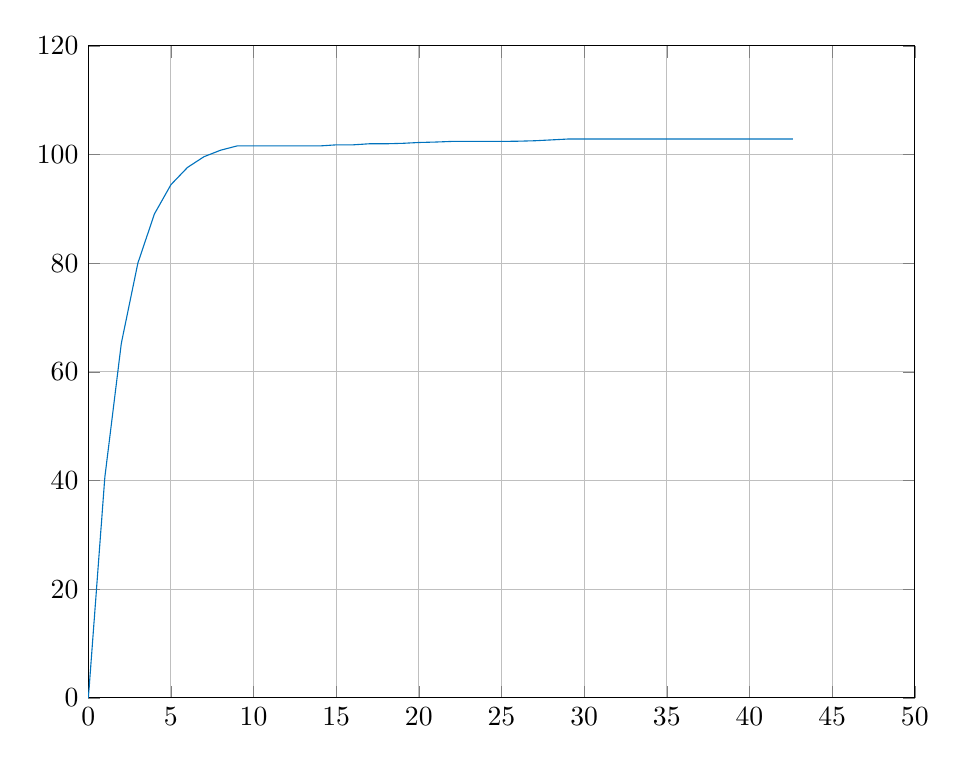
\begin{tikzpicture}

\begin{axis}[%
width=4.133in,
height=3.26in,
at={(0.693in,0.44in)},
scale only axis,
xmin=0,
xmax=50,
xmajorgrids,
ymin=0,
ymax=120,
ymajorgrids,
axis background/.style={fill=white}
]
\addplot [color=mycolor1,solid,forget plot]
  table[row sep=crcr]{%
0	0\\
0.018049959999999	0.336\\
0.0298611209999993	0.822\\
0.0451462420000006	1.394\\
0.0632602809999995	2.016\\
0.0782970130000003	2.678\\
0.0934459829999991	3.318\\
0.109304623	3.956\\
0.125296311999999	4.604\\
0.143715356000001	5.284\\
0.157172234999999	5.914\\
0.173103023	6.56\\
0.189293802999999	7.214\\
0.205321816	7.864\\
0.221265666999999	8.518\\
0.237188444	9.17\\
0.253097583000001	9.824\\
0.269345741	10.476\\
0.285232345000001	11.136\\
0.301338317	11.786\\
0.317272335999999	12.448\\
0.333290343	13.104\\
0.349264617000001	13.774\\
0.367697738	14.444\\
0.383016511	15.086\\
0.398235614	15.72\\
0.413700511	16.364\\
0.429331499	17.012\\
0.4473145	17.684\\
0.462583238	18.334\\
0.478608732999999	18.98\\
0.493826169	19.634\\
0.509335162000001	20.282\\
0.525141999	20.928\\
0.543410120999999	21.632\\
0.558528377	22.27\\
0.573703407	22.912\\
0.589291639	23.55\\
0.605314296	24.192\\
0.621198641000001	24.85\\
0.637272888	25.498\\
0.653264243000001	26.156\\
0.669203438999999	26.82\\
0.685274003	27.486\\
0.701384311999999	28.132\\
0.717264058	28.778\\
0.733322790999999	29.422\\
0.749260975	30.106\\
0.765319852	30.742\\
0.781211106000001	31.394\\
0.799545405999999	32.06\\
0.814694749	32.706\\
0.829836959999999	33.348\\
0.845754808	34.022\\
0.861289422	34.67\\
0.877243589	35.324\\
0.893275267999999	35.964\\
0.909321165999999	36.608\\
0.925390623	37.29\\
0.941294483999999	37.932\\
0.957161721999999	38.594\\
0.973278391000001	39.266\\
0.989272345999999	39.898\\
1.005295096	40.488\\
1.022747789	41.01\\
1.037623824	41.338\\
1.053156006	41.716\\
1.069183578	42.122\\
1.085178054	42.514\\
1.101158561	42.922\\
1.117284876	43.31\\
1.133316838	43.716\\
1.149271805	44.104\\
1.165474443	44.492\\
1.181208389	44.894\\
1.19746945	45.288\\
1.213302891	45.678\\
1.229326469	46.068\\
1.245285024	46.464\\
1.261329348	46.864\\
1.277322246	47.258\\
1.293317257	47.656\\
1.309286117	48.064\\
1.325404409	48.456\\
1.341281853	48.844\\
1.357277232	49.238\\
1.373181497	49.634\\
1.389327164	50.028\\
1.405299492	50.422\\
1.421240173	50.822\\
1.437325489	51.212\\
1.453300521	51.612\\
1.469356256	52.006\\
1.485249605	52.4\\
1.501314971	52.796\\
1.517244759	53.208\\
1.533319775	53.596\\
1.549248969	53.99\\
1.565422335	54.38\\
1.581264767	54.774\\
1.59735806	55.172\\
1.613267197	55.574\\
1.629572562	55.962\\
1.64527421	56.362\\
1.661237523	56.754\\
1.677329899	57.148\\
1.693284783	57.548\\
1.709247676	57.94\\
1.725386585	58.338\\
1.74132328	58.746\\
1.75739648	59.138\\
1.773274182	59.534\\
1.789262894	59.93\\
1.805291289	60.316\\
1.821231673	60.71\\
1.837337583	61.108\\
1.85322714	61.53\\
1.869272951	61.934\\
1.885268508	62.318\\
1.901374702	62.702\\
1.917283439	63.096\\
1.933395237	63.486\\
1.949252412	63.882\\
1.965310269	64.276\\
1.981337468	64.67\\
1.997270069	65.07\\
2.018034165	65.406\\
2.029768007	65.624\\
2.045122018	65.848\\
2.063227873	66.096\\
2.07824483	66.33\\
2.093211942	66.56\\
2.109218124	66.798\\
2.125348714	67.044\\
2.141185682	67.286\\
2.157369976	67.512\\
2.173338002	67.742\\
2.189254262	67.974\\
2.205200358	68.208\\
2.221319989	68.442\\
2.237319937	68.686\\
2.253218588	68.92\\
2.269448005	69.158\\
2.285254281	69.386\\
2.301244768	69.622\\
2.317296955	69.864\\
2.333470367	70.098\\
2.349295606	70.342\\
2.365403709	70.572\\
2.381188904	70.806\\
2.397323977	71.048\\
2.413294259	71.278\\
2.429338047	71.512\\
2.445315349	71.75\\
2.461323657	71.99\\
2.477177595	72.226\\
2.493355026	72.47\\
2.509174987	72.7\\
2.525314297	72.94\\
2.541340718	73.174\\
2.557278419	73.406\\
2.573194472	73.636\\
2.589298102	73.88\\
2.60531541	74.116\\
2.621232255	74.348\\
2.637375267	74.58\\
2.653369028	74.818\\
2.669298082	75.054\\
2.685131142	75.286\\
2.701298972	75.524\\
2.717262954	75.772\\
2.73343679	76\\
2.749182731	76.248\\
2.76546499	76.472\\
2.781233895	76.704\\
2.797459918	76.936\\
2.813243269	77.174\\
2.829376965	77.41\\
2.845351634	77.648\\
2.861324725	77.88\\
2.877339277	78.116\\
2.893342163	78.36\\
2.9092666	78.592\\
2.925358147	78.828\\
2.94130044	79.072\\
2.957392999	79.304\\
2.973293542	79.536\\
2.989278432	79.768\\
3.005270734	79.998\\
3.022810477	80.166\\
3.037778761	80.304\\
3.053155996	80.444\\
3.071320461	80.596\\
3.086381436	80.736\\
3.101413342	80.876\\
3.117267956	81.018\\
3.133235313	81.166\\
3.149264577	81.308\\
3.165592899	81.452\\
3.181209447	81.596\\
3.199676442	81.748\\
3.214840262	81.89\\
3.230102445	82.038\\
3.245362193	82.182\\
3.261416494	82.322\\
3.277277819	82.462\\
3.293326678	82.614\\
3.309270725	82.758\\
3.325296037	82.9\\
3.341183699	83.042\\
3.357271706	83.194\\
3.373306883	83.344\\
3.389244302	83.49\\
3.405165865	83.628\\
3.421295976	83.772\\
3.437340611	83.92\\
3.453302112	84.064\\
3.469816883	84.204\\
3.485226926	84.352\\
3.503758902	84.496\\
3.519063364	84.644\\
3.534156719	84.784\\
3.549238874	84.93\\
3.565356507	85.074\\
3.581218215	85.218\\
3.599544799	85.364\\
3.614694783	85.504\\
3.629854393	85.648\\
3.645289673	85.79\\
3.661261468	85.938\\
3.67723372	86.08\\
3.693283516	86.224\\
3.709847514	86.372\\
3.725465675	86.518\\
3.74126326	86.666\\
3.757160985	86.808\\
3.773333695	86.948\\
3.789311288	87.092\\
3.805310927	87.238\\
3.821265578	87.384\\
3.837316297	87.526\\
3.853238172	87.672\\
3.869277398	87.818\\
3.885212508	87.964\\
3.901308774	88.106\\
3.917283036	88.25\\
3.933411441	88.4\\
3.949257419	88.542\\
3.965656771	88.684\\
3.981389108	88.832\\
3.997473034	88.976\\
4.018161327	89.106\\
4.029945157	89.182\\
4.045146557	89.268\\
4.063317339	89.358\\
4.078356158	89.44\\
4.093399063	89.528\\
4.109171737	89.612\\
4.125385421	89.696\\
4.14132151	89.782\\
4.157404597	89.868\\
4.173621202	89.956\\
4.189236549	90.038\\
4.20529777	90.124\\
4.22120409	90.214\\
4.237484849	90.3\\
4.253290215	90.382\\
4.269354373	90.47\\
4.285189649	90.558\\
4.301366367	90.644\\
4.317221439	90.728\\
4.333421594	90.814\\
4.349349563	90.904\\
4.365363477	90.99\\
4.381256318	91.074\\
4.39755843	91.162\\
4.413259264	91.246\\
4.42965371	91.334\\
4.445294535	91.418\\
4.461376435	91.504\\
4.477294516	91.592\\
4.49331114	91.68\\
4.509346313	91.766\\
4.52526558	91.85\\
4.541311124	91.94\\
4.557188821	92.028\\
4.573311416	92.112\\
4.589369823	92.194\\
4.605422449	92.282\\
4.621277676	92.368\\
4.637288856	92.456\\
4.653298597	92.538\\
4.669336071	92.63\\
4.685285661	92.714\\
4.701229778	92.802\\
4.717210653	92.888\\
4.733278456	92.972\\
4.749248824	93.06\\
4.765423808	93.146\\
4.781224184	93.23\\
4.797466122	93.316\\
4.813203908	93.404\\
4.829266884	93.492\\
4.84530269	93.576\\
4.861244283	93.664\\
4.877351432	93.754\\
4.893280797	93.84\\
4.909258991	93.926\\
4.925221214	94.014\\
4.941347241	94.098\\
4.957530059	94.182\\
4.973327131	94.264\\
4.989328071	94.35\\
5.005297292	94.432\\
5.022657473	94.492\\
5.037619528	94.544\\
5.053223653	94.594\\
5.069182527	94.644\\
5.085190518	94.692\\
5.10136798	94.746\\
5.117182936	94.798\\
5.133296075	94.846\\
5.149265917	94.894\\
5.165433997	94.944\\
5.181250501	94.998\\
5.197522807	95.05\\
5.213204085	95.1\\
5.229278132	95.15\\
5.245212942	95.2\\
5.261321276	95.252\\
5.277226652	95.302\\
5.293253856	95.354\\
5.30926006	95.402\\
5.325295183	95.454\\
5.341334236	95.506\\
5.357486409	95.558\\
5.37323629	95.606\\
5.38929032	95.654\\
5.405296281	95.708\\
5.421291885	95.758\\
5.43723944	95.812\\
5.45327303	95.862\\
5.469316217	95.91\\
5.48525196	95.958\\
5.501146791	96.014\\
5.517100745	96.062\\
5.533113926	96.114\\
5.549090136	96.168\\
5.565354071	96.218\\
5.581306213	96.266\\
5.597544669	96.316\\
5.613295208	96.368\\
5.629292919	96.42\\
5.645327047	96.472\\
5.661325076	96.52\\
5.677154371	96.57\\
5.693313768	96.618\\
5.709199147	96.672\\
5.725312167	96.722\\
5.741171392	96.772\\
5.75731581	96.828\\
5.773323966	96.876\\
5.789275255	96.926\\
5.805150298	96.974\\
5.821270046	97.026\\
5.837122081	97.076\\
5.853105291	97.128\\
5.869311146	97.178\\
5.885290077	97.23\\
5.901263611	97.28\\
5.917310421	97.33\\
5.93339979	97.38\\
5.949251832	97.432\\
5.965420643	97.482\\
5.981352648	97.534\\
5.997458743	97.588\\
6.01830534	97.63\\
6.030067946	97.66\\
6.04514202	97.69\\
6.063299539	97.72\\
6.078236259	97.756\\
6.093342528	97.786\\
6.109281	97.818\\
6.125384624	97.848\\
6.141272821	97.88\\
6.157303115	97.912\\
6.173233037	97.942\\
6.18928169	97.978\\
6.205300827	98.008\\
6.221282149	98.038\\
6.23733624	98.07\\
6.253184248	98.1\\
6.269195906	98.134\\
6.285224412	98.166\\
6.303725554	98.2\\
6.319015785	98.23\\
6.334264282	98.262\\
6.349585418	98.294\\
6.365424117	98.326\\
6.381238683	98.358\\
6.399812666	98.39\\
6.415134965	98.42\\
6.430289503	98.45\\
6.44566181	98.484\\
6.461341318	98.514\\
6.477269375	98.548\\
6.493326042	98.578\\
6.509291864	98.61\\
6.525513514	98.64\\
6.541301087	98.672\\
6.557351571	98.704\\
6.5733119	98.738\\
6.589306707	98.768\\
6.605167639	98.8\\
6.621283588	98.83\\
6.637301828	98.862\\
6.653336128	98.894\\
6.669500827	98.928\\
6.685174036	98.958\\
6.701401491	98.994\\
6.717269399	99.024\\
6.733417269	99.056\\
6.749247524	99.086\\
6.765368944	99.118\\
6.7813904	99.148\\
6.799731116	99.18\\
6.815072243	99.21\\
6.83013689	99.246\\
6.845504355	99.276\\
6.861264956	99.308\\
6.877246642	99.338\\
6.893296415	99.372\\
6.909255452	99.4\\
6.925372856	99.432\\
6.941306941	99.466\\
6.959801686	99.5\\
6.975063629	99.53\\
6.990216884	99.564\\
7.005422504	99.592\\
7.021112294	99.61\\
7.039254781	99.632\\
7.054245879	99.65\\
7.069144548	99.668\\
7.085171911	99.686\\
7.101164434	99.706\\
7.117297905	99.726\\
7.133313926	99.744\\
7.14924971	99.762\\
7.165462898	99.782\\
7.181311772	99.802\\
7.199671096	99.824\\
7.213318852	99.838\\
7.229272846	99.856\\
7.24526155	99.876\\
7.261313943	99.896\\
7.277243682	99.916\\
7.293389016	99.934\\
7.309210264	99.952\\
7.327682144	99.974\\
7.343014074	99.996\\
7.358371332	100.012\\
7.374590511	100.03\\
7.389881926	100.046\\
7.405315036	100.066\\
7.421235296	100.086\\
7.437192794	100.106\\
7.453254371	100.126\\
7.469525314	100.144\\
7.485266099	100.162\\
7.501367104	100.182\\
7.51726007	100.202\\
7.533246346	100.22\\
7.54932269	100.236\\
7.565507061	100.256\\
7.581349709	100.276\\
7.597248819	100.296\\
7.61321916	100.316\\
7.629263259	100.334\\
7.645240038	100.352\\
7.661360509	100.372\\
7.677322381	100.392\\
7.693369407	100.41\\
7.709281346	100.426\\
7.725213865	100.446\\
7.741307644	100.466\\
7.759724964	100.486\\
7.774965189	100.506\\
7.790171929	100.524\\
7.806019789	100.544\\
7.821310386	100.562\\
7.837414666	100.582\\
7.853331917	100.602\\
7.869113916	100.618\\
7.885263686	100.636\\
7.901371215	100.656\\
7.917184787	100.676\\
7.933224291	100.696\\
7.94921875	100.714\\
7.965332657	100.732\\
7.981308696	100.752\\
7.99731497	100.772\\
8.017946108	100.788\\
8.029690564	100.8\\
8.045147235	100.816\\
8.063239912	100.826\\
8.078195708	100.836\\
8.093195867	100.852\\
8.109268168	100.866\\
8.125318911	100.876\\
8.141339673	100.886\\
8.157212474	100.902\\
8.173463521	100.916\\
8.189264163	100.926\\
8.205207964	100.938\\
8.22126796	100.952\\
8.237299139	100.966\\
8.253216232	100.976\\
8.269290313	100.988\\
8.285238027	101.004\\
8.301315092	101.016\\
8.317257916	101.026\\
8.333218156	101.04\\
8.349270102	101.056\\
8.365528066	101.066\\
8.381296957	101.076\\
8.399906511	101.092\\
8.41528594	101.106\\
8.430629968	101.116\\
8.445752769	101.13\\
8.46132073	101.142\\
8.477150156	101.156\\
8.493291201	101.166\\
8.509228316	101.178\\
8.525298574	101.196\\
8.541326167	101.206\\
8.557338875	101.218\\
8.573347048	101.232\\
8.58933537	101.246\\
8.605201743	101.256\\
8.621253954	101.266\\
8.637284755	101.282\\
8.653267422	101.296\\
8.669136427	101.306\\
8.685406706	101.316\\
8.701313484	101.336\\
8.717223374	101.346\\
8.733340187	101.356\\
8.749194226	101.372\\
8.765357765	101.384\\
8.781212356	101.396\\
8.797360459	101.406\\
8.81329928	101.422\\
8.829273837	101.436\\
8.845250512	101.446\\
8.861299397	101.456\\
8.877285188	101.474\\
8.893366663	101.486\\
8.909373673	101.496\\
8.925360327	101.506\\
8.94126218	101.526\\
8.957251648	101.536\\
8.973543678	101.546\\
8.989389058	101.56\\
9.005329086	101.57\\
9.021121089	101.57\\
9.037140076	101.57\\
9.053150566	101.57\\
9.069191585	101.57\\
9.085198501	101.57\\
9.101313705	101.57\\
9.117311268	101.57\\
9.133416821	101.57\\
9.149332565	101.57\\
9.165325237	101.57\\
9.181239468	101.57\\
9.197376688	101.57\\
9.213320936	101.57\\
9.229294258	101.57\\
9.245421957	101.57\\
9.26129978	101.57\\
9.277259747	101.57\\
9.293197734	101.57\\
9.309194602	101.57\\
9.325363015	101.57\\
9.341168096	101.57\\
9.357209895	101.57\\
9.373382705	101.57\\
9.389309142	101.57\\
9.405312338	101.57\\
9.421318957	101.57\\
9.437412674	101.57\\
9.453295112	101.57\\
9.469247973	101.57\\
9.485196618	101.57\\
9.501309145	101.57\\
9.517165242	101.57\\
9.533378335	101.57\\
9.549274519	101.57\\
9.565289201	101.57\\
9.581496906	101.57\\
9.597171251	101.57\\
9.61321155	101.57\\
9.629324236	101.57\\
9.645297866	101.57\\
9.661293485	101.57\\
9.677270322	101.57\\
9.693364163	101.57\\
9.709239094	101.57\\
9.725246008	101.57\\
9.741294046	101.57\\
9.757436343	101.57\\
9.773324161	101.57\\
9.789316299	101.57\\
9.80530825	101.57\\
9.821308649	101.57\\
9.837345367	101.57\\
9.853247164	101.57\\
9.869246378	101.57\\
9.885310086	101.57\\
9.901301328	101.57\\
9.917217525	101.57\\
9.933306347	101.57\\
9.94923508	101.57\\
9.96525085	101.57\\
9.981471073	101.57\\
9.997704656	101.57\\
10.018462308	101.57\\
10.03023609	101.57\\
10.04523099	101.57\\
10.063368843	101.57\\
10.078320204	101.57\\
10.093418803	101.57\\
10.109232499	101.57\\
10.125251452	101.57\\
10.141358824	101.57\\
10.157433516	101.57\\
10.173204131	101.57\\
10.189306192	101.57\\
10.205247403	101.57\\
10.221167589	101.57\\
10.237246553	101.57\\
10.25331407	101.57\\
10.269649897	101.57\\
10.285261054	101.57\\
10.301247517	101.57\\
10.317193189	101.57\\
10.33326511	101.57\\
10.349443954	101.57\\
10.365189386	101.57\\
10.381493113	101.57\\
10.397201303	101.57\\
10.413582514	101.57\\
10.429246912	101.57\\
10.44531232	101.57\\
10.461168617	101.57\\
10.47719007	101.57\\
10.493229977	101.57\\
10.509347333	101.57\\
10.52530116	101.57\\
10.541219682	101.57\\
10.557248759	101.57\\
10.573330618	101.57\\
10.589268087	101.57\\
10.60530111	101.57\\
10.621341541	101.57\\
10.637332855	101.57\\
10.653302675	101.57\\
10.669277362	101.57\\
10.685274196	101.57\\
10.701433811	101.57\\
10.717365734	101.57\\
10.733270635	101.57\\
10.749417525	101.57\\
10.765299291	101.57\\
10.783783387	101.57\\
10.798997998	101.57\\
10.81431488	101.57\\
10.829752188	101.57\\
10.847019531	101.57\\
10.862154883	101.57\\
10.877255054	101.57\\
10.893265602	101.57\\
10.909262499	101.57\\
10.925228701	101.57\\
10.941256528	101.57\\
10.95952899	101.57\\
10.974673937	101.57\\
10.990021631	101.57\\
11.005343446	101.57\\
11.022871411	101.57\\
11.038508339	101.57\\
11.05381425	101.57\\
11.069238915	101.57\\
11.085337767	101.57\\
11.10129937	101.57\\
11.117307262	101.57\\
11.133262184	101.57\\
11.149428094	101.57\\
11.165261064	101.57\\
11.181615702	101.57\\
11.197273666	101.57\\
11.215592097	101.57\\
11.230866327	101.57\\
11.24613272	101.57\\
11.261489395	101.57\\
11.277396795	101.57\\
11.293231661	101.57\\
11.309219074	101.57\\
11.325213982	101.57\\
11.341308711	101.57\\
11.357253401	101.57\\
11.373248669	101.57\\
11.389341605	101.57\\
11.405335594	101.57\\
11.421369077	101.57\\
11.437257535	101.57\\
11.453207083	101.57\\
11.469205749	101.57\\
11.485301685	101.57\\
11.501323421	101.57\\
11.517348777	101.57\\
11.533282882	101.57\\
11.549457521	101.57\\
11.565301592	101.57\\
11.581601902	101.57\\
11.597247192	101.57\\
11.613282358	101.57\\
11.629303643	101.57\\
11.645288052	101.57\\
11.661260744	101.57\\
11.677342203	101.57\\
11.693317213	101.57\\
11.709346069	101.57\\
11.725336036	101.57\\
11.741291298	101.57\\
11.757326253	101.57\\
11.773235173	101.57\\
11.789378503	101.57\\
11.805280976	101.57\\
11.821237656	101.57\\
11.837227943	101.57\\
11.85332284	101.57\\
11.869262245	101.57\\
11.885310383	101.57\\
11.901291504	101.57\\
11.917304688	101.57\\
11.933213521	101.57\\
11.949409188	101.57\\
11.965236796	101.57\\
11.981465418	101.57\\
11.997198592	101.57\\
12.02153037	101.57\\
12.031698849	101.57\\
12.047031542	101.57\\
12.062380511	101.57\\
12.077743372	101.57\\
12.093317514	101.57\\
12.109287998	101.57\\
12.125299378	101.57\\
12.141420147	101.57\\
12.157452268	101.57\\
12.173207375	101.57\\
12.189187807	101.57\\
12.205344877	101.57\\
12.221402456	101.57\\
12.237288401	101.57\\
12.253306326	101.57\\
12.269269276	101.57\\
12.285438373	101.57\\
12.301314948	101.57\\
12.317253677	101.57\\
12.333282662	101.57\\
12.349357069	101.57\\
12.365237293	101.57\\
12.38141747	101.57\\
12.39713934	101.57\\
12.413354054	101.57\\
12.429338619	101.57\\
12.445268318	101.57\\
12.461189222	101.57\\
12.477315452	101.57\\
12.493240126	101.57\\
12.509224892	101.57\\
12.525343585	101.57\\
12.54125862	101.57\\
12.558337626	101.57\\
12.573663461	101.57\\
12.589317556	101.57\\
12.605365925	101.57\\
12.621359158	101.57\\
12.637231611	101.57\\
12.653330567	101.57\\
12.669334337	101.57\\
12.685338307	101.57\\
12.701277559	101.57\\
12.717311184	101.57\\
12.73331598	101.57\\
12.749445157	101.57\\
12.765222426	101.57\\
12.783609887	101.57\\
12.797303792	101.57\\
12.8136322	101.57\\
12.829306672	101.57\\
12.845342773	101.57\\
12.861300097	101.57\\
12.877369972	101.57\\
12.893242828	101.57\\
12.909233771	101.57\\
12.925278948	101.57\\
12.941364157	101.57\\
12.957273081	101.57\\
12.973275467	101.57\\
12.989197714	101.57\\
13.005147465	101.57\\
13.022758444	101.57\\
13.037839376	101.57\\
13.053429857	101.57\\
13.069256438	101.57\\
13.0853721	101.57\\
13.101293465	101.57\\
13.117327601	101.57\\
13.133880664	101.57\\
13.149553166	101.57\\
13.165227583	101.57\\
13.183804478	101.57\\
13.198899873	101.57\\
13.214107031	101.57\\
13.229286331	101.57\\
13.245283825	101.57\\
13.261191344	101.57\\
13.277325562	101.57\\
13.293103026	101.57\\
13.309333513	101.57\\
13.325353984	101.57\\
13.341274124	101.57\\
13.357243312	101.57\\
13.373346324	101.57\\
13.389117842	101.57\\
13.405294073	101.57\\
13.421249977	101.57\\
13.437323473	101.57\\
13.453352863	101.57\\
13.469319542	101.57\\
13.485297145	101.57\\
13.501295851	101.57\\
13.517338763	101.57\\
13.533481014	101.57\\
13.549387586	101.57\\
13.565167999	101.57\\
13.583540504	101.57\\
13.598664461	101.57\\
13.613989892	101.57\\
13.62936468	101.57\\
13.645245261	101.57\\
13.661278492	101.57\\
13.677404717	101.57\\
13.69330916	101.57\\
13.709424425	101.57\\
13.725337635	101.57\\
13.741375517	101.57\\
13.759690631	101.57\\
13.774940044	101.57\\
13.790144645	101.57\\
13.805456096	101.57\\
13.821339659	101.57\\
13.83731382	101.57\\
13.853174658	101.57\\
13.869266337	101.57\\
13.885298639	101.57\\
13.901257049	101.57\\
13.917440037	101.57\\
13.933216716	101.57\\
13.949302334	101.57\\
13.965252815	101.57\\
13.981326814	101.57\\
13.997213162	101.57\\
14.022088657	101.574\\
14.030778285	101.58\\
14.045938495	101.58\\
14.061258408	101.58\\
14.077355643	101.59\\
14.093299459	101.59\\
14.109313524	101.59\\
14.125199495	101.6\\
14.141190536	101.6\\
14.157353459	101.6\\
14.173276284	101.606\\
14.189295869	101.61\\
14.205254309	101.61\\
14.221342639	101.614\\
14.23734839	101.62\\
14.253298918	101.62\\
14.269288378	101.624\\
14.285338736	101.63\\
14.301300809	101.63\\
14.317356019	101.632\\
14.33326911	101.64\\
14.349351957	101.64\\
14.365302855	101.642\\
14.38361657	101.65\\
14.398861739	101.65\\
14.414465986	101.65\\
14.42965563	101.66\\
14.445286287	101.66\\
14.461238464	101.66\\
14.47728636	101.668\\
14.49323792	101.67\\
14.509297143	101.67\\
14.525307756	101.676\\
14.541388959	101.68\\
14.557486574	101.68\\
14.573843797	101.684\\
14.589401324	101.69\\
14.605299297	101.69\\
14.621306357	101.692\\
14.637299871	101.7\\
14.653336223	101.7\\
14.669241005	101.702\\
14.685331264	101.71\\
14.701287218	101.71\\
14.717486189	101.71\\
14.733264525	101.72\\
14.749191382	101.72\\
14.765305541	101.72\\
14.781473977	101.73\\
14.79716113	101.73\\
14.815663535	101.73\\
14.830994841	101.738\\
14.846196991	101.74\\
14.861616216	101.74\\
14.877326791	101.746\\
14.893288436	101.75\\
14.909355007	101.75\\
14.925332367	101.754\\
14.941346659	101.76\\
14.957334346	101.76\\
14.973266097	101.762\\
14.989710536	101.77\\
15.005241374	101.77\\
15.022829649	101.77\\
15.038198333	101.77\\
15.053632767	101.77\\
15.069424867	101.77\\
15.085353001	101.77\\
15.101281383	101.77\\
15.117320395	101.77\\
15.13331198	101.77\\
15.149326766	101.77\\
15.1651969	101.77\\
15.181422395	101.77\\
15.197305289	101.77\\
15.215647785	101.77\\
15.230772361	101.77\\
15.245977038	101.77\\
15.262142828	101.77\\
15.277341953	101.77\\
15.293303185	101.77\\
15.309250666	101.77\\
15.325312501	101.77\\
15.341298651	101.77\\
15.357320339	101.77\\
15.373314359	101.77\\
15.389309178	101.77\\
15.405265732	101.77\\
15.421344028	101.77\\
15.43726473	101.77\\
15.453335482	101.77\\
15.469341314	101.77\\
15.485122939	101.77\\
15.501283577	101.77\\
15.517332532	101.77\\
15.533232414	101.77\\
15.549411398	101.77\\
15.565270979	101.77\\
15.581430339	101.77\\
15.597134534	101.77\\
15.613458115	101.77\\
15.629278642	101.77\\
15.64535741	101.77\\
15.661326374	101.77\\
15.677355504	101.77\\
15.695360991	101.77\\
15.710626485	101.77\\
15.72637657	101.77\\
15.741676365	101.77\\
15.757446169	101.77\\
15.773263029	101.77\\
15.789302766	101.77\\
15.805258	101.77\\
15.821227756	101.77\\
15.837287705	101.77\\
15.853400645	101.77\\
15.869296754	101.77\\
15.885353693	101.77\\
15.90129592	101.77\\
15.917365427	101.77\\
15.933287274	101.77\\
15.949354966	101.77\\
15.965415971	101.77\\
15.981544468	101.77\\
15.997295789	101.77\\
16.018974063	101.77\\
16.030882145	101.776\\
16.046196255	101.78\\
16.061412691	101.78\\
16.077467884	101.784\\
16.093251703	101.79\\
16.109298859	101.79\\
16.1253121	101.79\\
16.141370259	101.8\\
16.157174756	101.8\\
16.173282252	101.8\\
16.189132942	101.81\\
16.205294388	101.81\\
16.221272517	101.81\\
16.237450505	101.82\\
16.253132408	101.82\\
16.269289173	101.82\\
16.285346381	101.828\\
16.301197488	101.83\\
16.317260144	101.83\\
16.333332318	101.836\\
16.349156743	101.84\\
16.365101246	101.84\\
16.381128889	101.844\\
16.397257904	101.85\\
16.413537658	101.85\\
16.429277919	101.854\\
16.445271311	101.86\\
16.461263092	101.86\\
16.477251668	101.86\\
16.494650156	101.87\\
16.509575386	101.87\\
16.525328105	101.87\\
16.541133166	101.88\\
16.55712356	101.88\\
16.573156511	101.88\\
16.58920278	101.888\\
16.605291287	101.89\\
16.621389002	101.89\\
16.637311909	101.898\\
16.653436037	101.9\\
16.669260112	101.9\\
16.685176397	101.904\\
16.701191861	101.91\\
16.717416208	101.91\\
16.733371791	101.914\\
16.749450223	101.92\\
16.765273507	101.92\\
16.781460655	101.922\\
16.797406453	101.93\\
16.813526597	101.93\\
16.82919888	101.93\\
16.845238026	101.94\\
16.861260602	101.94\\
16.877293741	101.94\\
16.893253784	101.95\\
16.909363767	101.95\\
16.925206996	101.95\\
16.943545959	101.958\\
16.958735983	101.96\\
16.973856355	101.96\\
16.989277312	101.966\\
17.005248991	101.97\\
17.022798135	101.97\\
17.038008177	101.97\\
17.053294929	101.97\\
17.069250055	101.97\\
17.085257068	101.97\\
17.101305453	101.97\\
17.117355195	101.97\\
17.133296561	101.97\\
17.149267025	101.97\\
17.16522648	101.97\\
17.181244335	101.97\\
17.197283799	101.97\\
17.213600229	101.97\\
17.229249489	101.97\\
17.245372241	101.97\\
17.261218435	101.97\\
17.277350092	101.97\\
17.293308825	101.97\\
17.30935577	101.97\\
17.325297678	101.97\\
17.341296336	101.97\\
17.357473252	101.97\\
17.373262022	101.97\\
17.389295439	101.97\\
17.405211426	101.97\\
17.421310154	101.97\\
17.437245275	101.97\\
17.453354798	101.97\\
17.469171322	101.97\\
17.485355774	101.97\\
17.501286852	101.97\\
17.517320993	101.97\\
17.533252763	101.97\\
17.549349118	101.97\\
17.565229668	101.97\\
17.581333187	101.97\\
17.597359917	101.97\\
17.613351737	101.97\\
17.629299388	101.97\\
17.645356696	101.97\\
17.661115973	101.97\\
17.6773569	101.97\\
17.693226133	101.97\\
17.709345317	101.97\\
17.725335306	101.97\\
17.741175939	101.97\\
17.757293962	101.97\\
17.773128422	101.97\\
17.789330313	101.97\\
17.805302634	101.97\\
17.821302333	101.97\\
17.837296679	101.97\\
17.85325784	101.97\\
17.869275609	101.97\\
17.885323769	101.97\\
17.901263014	101.97\\
17.917309493	101.97\\
17.93320142	101.97\\
17.949384705	101.97\\
17.9652743	101.97\\
17.981442004	101.97\\
17.9973271	101.97\\
18.021048869	101.97\\
18.029694453	101.972\\
18.045393085	101.974\\
18.061209476	101.974\\
18.07736963	101.976\\
18.09494873	101.978\\
18.110589984	101.978\\
18.125837923	101.978\\
18.141546103	101.982\\
18.157298193	101.982\\
18.17327524	101.982\\
18.189243383	101.986\\
18.205263456	101.986\\
18.22131424	101.986\\
18.237256945	101.988\\
18.25331289	101.99\\
18.26929771	101.99\\
18.285318802	101.992\\
18.301403514	101.994\\
18.317306361	101.994\\
18.333259756	101.996\\
18.349491721	101.998\\
18.365268999	101.998\\
18.383740607	102\\
18.399003015	102.002\\
18.414190528	102.002\\
18.42940119	102.004\\
18.445304595	102.006\\
18.461246376	102.006\\
18.477308958	102.006\\
18.493215336	102.008\\
18.509457056	102.01\\
18.527379543	102.01\\
18.542727222	102.012\\
18.55801168	102.014\\
18.573339114	102.014\\
18.589288495	102.016\\
18.605238888	102.018\\
18.621157277	102.018\\
18.63715217	102.02\\
18.65332871	102.022\\
18.669252223	102.022\\
18.6852232	102.024\\
18.701286148	102.026\\
18.717452453	102.026\\
18.733263474	102.028\\
18.749465764	102.03\\
18.765236391	102.03\\
18.781578394	102.03\\
18.797264342	102.034\\
18.813317191	102.034\\
18.829218897	102.034\\
18.845292182	102.036\\
18.861187929	102.038\\
18.879671657	102.038\\
18.894902457	102.04\\
18.910096179	102.042\\
18.925381444	102.042\\
18.941385232	102.044\\
18.957257371	102.046\\
18.973316725	102.046\\
18.989323497	102.048\\
19.005264838	102.05\\
19.022868583	102.05\\
19.038110161	102.052\\
19.053317738	102.058\\
19.069301335	102.058\\
19.085250828	102.06\\
19.101228648	102.066\\
19.117343671	102.066\\
19.133235444	102.066\\
19.149342458	102.072\\
19.165303261	102.074\\
19.181410832	102.074\\
19.197276869	102.08\\
19.213337743	102.082\\
19.229288477	102.082\\
19.245405232	102.088\\
19.261211359	102.09\\
19.27731164	102.09\\
19.293283355	102.096\\
19.309208045	102.098\\
19.325316804	102.098\\
19.341307311	102.102\\
19.357333878	102.106\\
19.373298204	102.106\\
19.390233156	102.108\\
19.405392165	102.114\\
19.421673644	102.114\\
19.437270046	102.114\\
19.453307355	102.122\\
19.469257982	102.122\\
19.485379551	102.122\\
19.501218149	102.128\\
19.517372643	102.13\\
19.533204837	102.13\\
19.549515655	102.136\\
19.565299798	102.138\\
19.583704998	102.138\\
19.598908829	102.144\\
19.614089644	102.146\\
19.629421552	102.146\\
19.645258363	102.152\\
19.661276327	102.154\\
19.677405604	102.154\\
19.69329648	102.156\\
19.709358239	102.162\\
19.725314825	102.162\\
19.741316916	102.164\\
19.757422737	102.17\\
19.773293278	102.17\\
19.790307069	102.17\\
19.80547588	102.176\\
19.821190589	102.178\\
19.83730669	102.178\\
19.853150009	102.184\\
19.86907144	102.186\\
19.885318108	102.186\\
19.901291181	102.192\\
19.917410517	102.194\\
19.933314822	102.194\\
19.949441493	102.2\\
19.965225232	102.202\\
19.981483441	102.202\\
19.997412799	102.206\\
20.021447159	102.208\\
20.030206022	102.208\\
20.04540507	102.208\\
20.061270516	102.212\\
20.077361484	102.212\\
20.09318007	102.212\\
20.109238877	102.216\\
20.125301861	102.216\\
20.14130635	102.216\\
20.157279604	102.22\\
20.173285627	102.22\\
20.189446663	102.22\\
20.205406102	102.224\\
20.221320919	102.224\\
20.237255865	102.224\\
20.25311034	102.228\\
20.269286097	102.228\\
20.285123209	102.228\\
20.301097416	102.232\\
20.317216326	102.232\\
20.333090014	102.232\\
20.351296551	102.234\\
20.366440746	102.236\\
20.382176036	102.236\\
20.397327944	102.236\\
20.413360612	102.24\\
20.429266913	102.24\\
20.44531249	102.24\\
20.461648305	102.244\\
20.477324722	102.244\\
20.494414005	102.244\\
20.509488536	102.248\\
20.525232526	102.248\\
20.541321756	102.248\\
20.557324591	102.252\\
20.573247042	102.252\\
20.589388257	102.252\\
20.605293117	102.256\\
20.621392807	102.256\\
20.637251747	102.256\\
20.653303378	102.258\\
20.66927397	102.26\\
20.685224361	102.26\\
20.701294264	102.26\\
20.71722885	102.264\\
20.733233386	102.264\\
20.749227187	102.264\\
20.76519732	102.268\\
20.783740478	102.268\\
20.798783037	102.268\\
20.814156713	102.272\\
20.829467715	102.272\\
20.845178183	102.272\\
20.86130794	102.276\\
20.877324702	102.276\\
20.893290769	102.276\\
20.909305408	102.28\\
20.925219546	102.28\\
20.941332721	102.28\\
20.957216846	102.284\\
20.973258212	102.284\\
20.989317815	102.284\\
21.005225575	102.286\\
21.021139691	102.288\\
21.039213686	102.288\\
21.054506027	102.29\\
21.069445652	102.294\\
21.085215197	102.294\\
21.10127656	102.296\\
21.117321505	102.3\\
21.133317756	102.3\\
21.149317615	102.302\\
21.165208131	102.306\\
21.181331477	102.306\\
21.197168382	102.308\\
21.213314729	102.312\\
21.229260746	102.312\\
21.245290006	102.314\\
21.261251794	102.318\\
21.277309263	102.318\\
21.293246049	102.318\\
21.309381359	102.32\\
21.325171616	102.324\\
21.341414617	102.324\\
21.357507088	102.326\\
21.373917819	102.33\\
21.38929142	102.33\\
21.405257212	102.332\\
21.421299076	102.336\\
21.437278939	102.336\\
21.453369599	102.338\\
21.469319324	102.342\\
21.485209483	102.342\\
21.501262363	102.344\\
21.517133659	102.348\\
21.533174411	102.348\\
21.549311722	102.35\\
21.565184259	102.354\\
21.581276922	102.354\\
21.597252109	102.356\\
21.615558101	102.36\\
21.630701843	102.36\\
21.645871865	102.36\\
21.66124042	102.362\\
21.677279275	102.366\\
21.693212393	102.366\\
21.709212201	102.368\\
21.72529577	102.372\\
21.741229741	102.372\\
21.757258067	102.374\\
21.773364482	102.378\\
21.789260638	102.378\\
21.805296286	102.38\\
21.82119195	102.384\\
21.837197508	102.384\\
21.853153771	102.386\\
21.869090015	102.39\\
21.885320586	102.39\\
21.901237203	102.392\\
21.917283315	102.396\\
21.933269367	102.396\\
21.951638528	102.396\\
21.966747108	102.402\\
21.981867209	102.402\\
21.997309995	102.402\\
22.021334739	102.404\\
22.029840741	102.404\\
22.045213116	102.404\\
22.061147494	102.404\\
22.077263989	102.404\\
22.093328336	102.404\\
22.109299295	102.404\\
22.125323772	102.404\\
22.141280735	102.404\\
22.157318971	102.404\\
22.173270921	102.404\\
22.189312449	102.404\\
22.205294713	102.404\\
22.221283922	102.404\\
22.237297382	102.404\\
22.253337668	102.404\\
22.269285468	102.404\\
22.28531737	102.404\\
22.301097929	102.404\\
22.317328653	102.404\\
22.333178923	102.404\\
22.351701325	102.404\\
22.367131769	102.404\\
22.382411247	102.404\\
22.397689686	102.404\\
22.41343989	102.404\\
22.429294559	102.404\\
22.445331833	102.404\\
22.461290909	102.404\\
22.477221665	102.404\\
22.493308151	102.404\\
22.509280643	102.404\\
22.525326621	102.404\\
22.541287982	102.404\\
22.557365823	102.404\\
22.573288279	102.404\\
22.589315938	102.404\\
22.605305347	102.404\\
22.621264439	102.404\\
22.637211951	102.404\\
22.653340058	102.404\\
22.669323625	102.404\\
22.685369981	102.404\\
22.701270363	102.404\\
22.717320305	102.404\\
22.733242798	102.404\\
22.749436055	102.404\\
22.765193064	102.404\\
22.781410179	102.404\\
22.79723841	102.404\\
22.813498047	102.404\\
22.829210248	102.404\\
22.845313998	102.404\\
22.861378377	102.404\\
22.877344941	102.404\\
22.893357639	102.404\\
22.909358775	102.404\\
22.925184444	102.404\\
22.941363319	102.404\\
22.957295399	102.404\\
22.973270817	102.404\\
22.989333944	102.404\\
23.005273806	102.404\\
23.022761769	102.404\\
23.037740246	102.404\\
23.053153677	102.404\\
23.069123881	102.404\\
23.087294963	102.404\\
23.102225798	102.404\\
23.117318171	102.404\\
23.133247625	102.404\\
23.149478572	102.404\\
23.165298669	102.404\\
23.18144731	102.404\\
23.197202208	102.404\\
23.213442619	102.404\\
23.229198228	102.404\\
23.245368492	102.404\\
23.261313246	102.404\\
23.277337315	102.404\\
23.293300756	102.404\\
23.309267675	102.404\\
23.325327665	102.404\\
23.341269419	102.404\\
23.35729349	102.404\\
23.373270728	102.404\\
23.389223674	102.404\\
23.405310837	102.404\\
23.421353703	102.404\\
23.437305023	102.404\\
23.453334813	102.404\\
23.46932956	102.404\\
23.485329048	102.404\\
23.501202837	102.404\\
23.517273661	102.404\\
23.5332935	102.404\\
23.549508056	102.404\\
23.565253991	102.404\\
23.58156876	102.404\\
23.597436578	102.404\\
23.613391722	102.404\\
23.629248046	102.404\\
23.645270551	102.404\\
23.661273892	102.404\\
23.67727639	102.404\\
23.693293234	102.404\\
23.709336436	102.404\\
23.725247358	102.404\\
23.741323813	102.404\\
23.757350159	102.404\\
23.773228652	102.404\\
23.789292522	102.404\\
23.805262432	102.404\\
23.821330626	102.404\\
23.837303019	102.404\\
23.853195898	102.404\\
23.869316105	102.404\\
23.88539541	102.404\\
23.901236396	102.404\\
23.917384126	102.404\\
23.93329761	102.404\\
23.949440618	102.404\\
23.965341433	102.404\\
23.981607548	102.404\\
23.997323605	102.404\\
24.021338573	102.404\\
24.029873026	102.404\\
24.045183487	102.404\\
24.061133357	102.404\\
24.079276491	102.404\\
24.094257061	102.404\\
24.109446085	102.404\\
24.125350555	102.404\\
24.141361677	102.404\\
24.157327504	102.404\\
24.175812211	102.404\\
24.191055791	102.404\\
24.206371044	102.404\\
24.221570692	102.404\\
24.2373213	102.404\\
24.253542745	102.404\\
24.26921745	102.404\\
24.285368677	102.404\\
24.301264788	102.404\\
24.317304863	102.404\\
24.333291176	102.404\\
24.349649235	102.404\\
24.365193604	102.404\\
24.383703547	102.404\\
24.398862476	102.404\\
24.414193681	102.404\\
24.429470205	102.404\\
24.445264881	102.404\\
24.461211836	102.404\\
24.477364051	102.404\\
24.493302919	102.404\\
24.509401119	102.404\\
24.525337028	102.404\\
24.541391636	102.404\\
24.557319681	102.404\\
24.573271987	102.404\\
24.589304555	102.404\\
24.605293159	102.404\\
24.621354654	102.404\\
24.637495573	102.404\\
24.6533501	102.404\\
24.669246844	102.404\\
24.685333886	102.404\\
24.701292762	102.404\\
24.71742603	102.404\\
24.733205904	102.404\\
24.749450255	102.404\\
24.765227597	102.404\\
24.781409381	102.404\\
24.797351961	102.404\\
24.813323402	102.404\\
24.829225301	102.404\\
24.845382503	102.404\\
24.861281561	102.404\\
24.877305129	102.404\\
24.894456911	102.404\\
24.909681873	102.404\\
24.925362005	102.404\\
24.941258949	102.404\\
24.957165018	102.404\\
24.973285986	102.404\\
24.991661253	102.404\\
25.006846507	102.404\\
25.021810321	102.404\\
25.037145467	102.404\\
25.053168958	102.406\\
25.069134208	102.406\\
25.085190124	102.406\\
25.103398122	102.408\\
25.118654422	102.408\\
25.133984296	102.408\\
25.149330525	102.408\\
25.165157861	102.41\\
25.181703182	102.41\\
25.19726782	102.41\\
25.213278091	102.412\\
25.229205424	102.412\\
25.245293545	102.412\\
25.261207834	102.414\\
25.277262858	102.414\\
25.293182396	102.414\\
25.309302361	102.416\\
25.325295936	102.416\\
25.343815803	102.416\\
25.359094863	102.418\\
25.374388387	102.418\\
25.389517795	102.418\\
25.405257379	102.42\\
25.421295283	102.42\\
25.437337383	102.42\\
25.453268771	102.422\\
25.469289793	102.422\\
25.48539698	102.422\\
25.501270232	102.424\\
25.517269739	102.424\\
25.53335807	102.424\\
25.549459753	102.424\\
25.565284248	102.426\\
25.581620256	102.426\\
25.59755901	102.426\\
25.613320775	102.428\\
25.629294516	102.428\\
25.645298136	102.428\\
25.661187109	102.43\\
25.677342896	102.43\\
25.693437469	102.43\\
25.709349338	102.432\\
25.725128377	102.432\\
25.743473684	102.432\\
25.75868887	102.434\\
25.774055765	102.434\\
25.789411214	102.434\\
25.805329918	102.436\\
25.821226837	102.436\\
25.837278871	102.436\\
25.853298569	102.436\\
25.869242371	102.438\\
25.885254413	102.438\\
25.901861001	102.438\\
25.917389509	102.44\\
25.9331604	102.44\\
25.949304848	102.44\\
25.965502695	102.442\\
25.981314463	102.442\\
25.99754932	102.442\\
26.021923868	102.446\\
26.030697107	102.446\\
26.04574969	102.446\\
26.061342116	102.45\\
26.077285296	102.45\\
26.093366569	102.45\\
26.10928407	102.454\\
26.125295526	102.454\\
26.141290083	102.454\\
26.157293069	102.456\\
26.173296415	102.458\\
26.189330715	102.458\\
26.205337167	102.458\\
26.221350756	102.462\\
26.23730451	102.462\\
26.25330743	102.462\\
26.269312571	102.466\\
26.28519346	102.466\\
26.30120504	102.466\\
26.317267686	102.47\\
26.33347065	102.47\\
26.349170195	102.47\\
26.367664929	102.474\\
26.38292422	102.474\\
26.398063244	102.474\\
26.41323418	102.478\\
26.429353604	102.478\\
26.445302516	102.478\\
26.461414924	102.478\\
26.477322295	102.482\\
26.49327051	102.482\\
26.509406155	102.482\\
26.525250551	102.486\\
26.541333918	102.486\\
26.557297305	102.486\\
26.573220822	102.49\\
26.589342945	102.49\\
26.605336199	102.49\\
26.621274304	102.494\\
26.63731916	102.494\\
26.653297163	102.494\\
26.669412172	102.498\\
26.685319879	102.498\\
26.701345148	102.498\\
26.717346044	102.502\\
26.73339977	102.502\\
26.749287404	102.502\\
26.765477459	102.506\\
26.781321956	102.506\\
26.797565261	102.506\\
26.813200937	102.506\\
26.829355915	102.51\\
26.84529325	102.51\\
26.861190228	102.51\\
26.877274255	102.514\\
26.89328362	102.514\\
26.909283972	102.514\\
26.925295252	102.518\\
26.941324146	102.518\\
26.957286134	102.518\\
26.97329816	102.522\\
26.989376772	102.522\\
27.005315679	102.522\\
27.021199771	102.528\\
27.037236115	102.528\\
27.053262409	102.53\\
27.069312232	102.536\\
27.085245569	102.536\\
27.10130359	102.538\\
27.117231576	102.542\\
27.133281954	102.544\\
27.149287466	102.546\\
27.165401623	102.546\\
27.181186451	102.552\\
27.197423163	102.552\\
27.213346851	102.554\\
27.229313996	102.56\\
27.245289454	102.56\\
27.261270155	102.562\\
27.277237068	102.568\\
27.293328936	102.568\\
27.309354528	102.57\\
27.325330457	102.576\\
27.341305274	102.576\\
27.357226383	102.578\\
27.373372569	102.584\\
27.389261564	102.584\\
27.405244143	102.586\\
27.421243464	102.592\\
27.437355912	102.592\\
27.453349162	102.594\\
27.469290062	102.598\\
27.485254751	102.6\\
27.501169177	102.602\\
27.5172906	102.602\\
27.533301153	102.608\\
27.549267706	102.608\\
27.565470349	102.61\\
27.581312345	102.616\\
27.597381195	102.616\\
27.613344586	102.618\\
27.629294788	102.624\\
27.645216478	102.624\\
27.66126792	102.626\\
27.677203761	102.632\\
27.693314544	102.632\\
27.709316808	102.634\\
27.725338809	102.64\\
27.741287972	102.64\\
27.757291221	102.642\\
27.773396143	102.646\\
27.789308673	102.648\\
27.805302144	102.65\\
27.821365431	102.65\\
27.837374225	102.656\\
27.853305919	102.658\\
27.869294282	102.658\\
27.88523192	102.664\\
27.901369525	102.664\\
27.917298514	102.666\\
27.933359721	102.672\\
27.949278386	102.672\\
27.96539574	102.674\\
27.981255638	102.68\\
27.997575757	102.68\\
28.018455135	102.684\\
28.030472376	102.688\\
28.045734374	102.688\\
28.061381075	102.69\\
28.077294066	102.696\\
28.093289395	102.696\\
28.109298523	102.698\\
28.125265192	102.702\\
28.141340495	102.704\\
28.157279411	102.706\\
28.173176902	102.708\\
28.18926213	102.712\\
28.205299644	102.712\\
28.221335534	102.716\\
28.237413785	102.72\\
28.253265634	102.72\\
28.269202135	102.724\\
28.285272959	102.728\\
28.3012567	102.728\\
28.317332572	102.732\\
28.333379192	102.736\\
28.349387789	102.736\\
28.36548763	102.738\\
28.38138434	102.744\\
28.39765183	102.744\\
28.413826429	102.746\\
28.429343825	102.75\\
28.445274036	102.752\\
28.461306387	102.754\\
28.477316866	102.756\\
28.493353759	102.76\\
28.509325415	102.76\\
28.52536841	102.764\\
28.541373372	102.768\\
28.557266739	102.768\\
28.573314635	102.772\\
28.589325684	102.776\\
28.605298016	102.776\\
28.621285391	102.78\\
28.637286021	102.784\\
28.653326698	102.784\\
28.669346557	102.788\\
28.685281613	102.792\\
28.703806121	102.792\\
28.719079434	102.794\\
28.734382725	102.8\\
28.749410336	102.8\\
28.765427103	102.802\\
28.7812561	102.806\\
28.797616638	102.808\\
28.813214734	102.81\\
28.829358043	102.812\\
28.845310565	102.816\\
28.86124944	102.816\\
28.877298736	102.82\\
28.893293582	102.824\\
28.90928815	102.824\\
28.925376358	102.828\\
28.941316717	102.832\\
28.957263811	102.832\\
28.973202278	102.836\\
28.98934092	102.84\\
29.005330224	102.84\\
29.022875201	102.84\\
29.038073479	102.84\\
29.053527179	102.84\\
29.069339927	102.84\\
29.085266687	102.84\\
29.101324515	102.84\\
29.117292141	102.84\\
29.13329886	102.84\\
29.149257856	102.84\\
29.165515945	102.84\\
29.18136358	102.84\\
29.197550772	102.84\\
29.213287239	102.84\\
29.229340291	102.84\\
29.245300061	102.84\\
29.261250097	102.84\\
29.277279584	102.84\\
29.293278074	102.84\\
29.309291212	102.84\\
29.325312468	102.84\\
29.341334809	102.84\\
29.357370012	102.84\\
29.374125274	102.84\\
29.389382224	102.84\\
29.405268627	102.84\\
29.421223273	102.84\\
29.437335851	102.84\\
29.45331077	102.84\\
29.469202882	102.84\\
29.485252779	102.84\\
29.501248668	102.84\\
29.517332949	102.84\\
29.533303286	102.84\\
29.549283629	102.84\\
29.565382388	102.84\\
29.581224771	102.84\\
29.597381048	102.84\\
29.613245435	102.84\\
29.629151866	102.84\\
29.645249001	102.84\\
29.661273857	102.84\\
29.677239618	102.84\\
29.693325652	102.84\\
29.710010763	102.84\\
29.725368742	102.84\\
29.741331517	102.84\\
29.757297103	102.84\\
29.773527514	102.84\\
29.789241797	102.84\\
29.805332561	102.84\\
29.821269662	102.84\\
29.837316839	102.84\\
29.85326086	102.84\\
29.869302073	102.84\\
29.885266988	102.84\\
29.901311096	102.84\\
29.917260165	102.84\\
29.933302762	102.84\\
29.949287214	102.84\\
29.965267093	102.84\\
29.981270484	102.84\\
29.999727835	102.84\\
30.017521201	102.84\\
30.029492185	102.84\\
30.045277592	102.84\\
30.061266881	102.84\\
30.077367837	102.84\\
30.093388109	102.84\\
30.109331961	102.84\\
30.125312796	102.84\\
30.141273215	102.84\\
30.157281995	102.84\\
30.173806577	102.84\\
30.189265786	102.84\\
30.205315929	102.84\\
30.221276288	102.84\\
30.237313967	102.84\\
30.253285146	102.84\\
30.269346564	102.84\\
30.285331534	102.84\\
30.301322478	102.84\\
30.317267773	102.84\\
30.333520384	102.84\\
30.349270176	102.84\\
30.365567313	102.84\\
30.381298484	102.84\\
30.39730352	102.84\\
30.413307036	102.84\\
30.429299974	102.84\\
30.445202697	102.84\\
30.461291468	102.84\\
30.477301334	102.84\\
30.493518431	102.84\\
30.509294822	102.84\\
30.525384933	102.84\\
30.541335162	102.84\\
30.557280567	102.84\\
30.57342276	102.84\\
30.589365726	102.84\\
30.605334015	102.84\\
30.621219825	102.84\\
30.637327077	102.84\\
30.653249762	102.84\\
30.669315108	102.84\\
30.685271403	102.84\\
30.701296666	102.84\\
30.717259384	102.84\\
30.73336768	102.84\\
30.749304841	102.84\\
30.765429061	102.84\\
30.781267263	102.84\\
30.797726523	102.84\\
30.813270626	102.84\\
30.829341138	102.84\\
30.845338502	102.84\\
30.86124433	102.84\\
30.877330802	102.84\\
30.893297264	102.84\\
30.909310278	102.84\\
30.925240554	102.84\\
30.941279892	102.84\\
30.957246007	102.84\\
30.973338523	102.84\\
30.98928026	102.84\\
31.005110585	102.84\\
31.022531201	102.84\\
31.037848449	102.84\\
31.053320803	102.84\\
31.069337705	102.84\\
31.085263529	102.84\\
31.101262544	102.84\\
31.117263424	102.84\\
31.133243776	102.84\\
31.149273612	102.84\\
31.165451011	102.84\\
31.181318505	102.84\\
31.199683647	102.84\\
31.214935922	102.84\\
31.230017415	102.84\\
31.245250327	102.84\\
31.261276916	102.84\\
31.277276885	102.84\\
31.293302672	102.84\\
31.309406847	102.84\\
31.325318376	102.84\\
31.34117478	102.84\\
31.3572661	102.84\\
31.37329601	102.84\\
31.389272318	102.84\\
31.405296812	102.84\\
31.421271358	102.84\\
31.437224881	102.84\\
31.453245543	102.84\\
31.469360525	102.84\\
31.485203428	102.84\\
31.50130932	102.84\\
31.517309491	102.84\\
31.533303835	102.84\\
31.549311566	102.84\\
31.565481872	102.84\\
31.581307957	102.84\\
31.597613701	102.84\\
31.613261032	102.84\\
31.629314554	102.84\\
31.64533976	102.84\\
31.661392453	102.84\\
31.677285119	102.84\\
31.693302157	102.84\\
31.709271241	102.84\\
31.725343173	102.84\\
31.741331435	102.84\\
31.757404505	102.84\\
31.77330558	102.84\\
31.789308469	102.84\\
31.805262536	102.84\\
31.821371321	102.84\\
31.837416372	102.84\\
31.853307258	102.84\\
31.869324378	102.84\\
31.885340512	102.84\\
31.901252444	102.84\\
31.917291095	102.84\\
31.933306021	102.84\\
31.94924207	102.84\\
31.965280743	102.84\\
31.981295627	102.84\\
31.997378817	102.84\\
32.018321808	102.84\\
32.030383274	102.84\\
32.045678999	102.84\\
32.061329651	102.84\\
32.077228028	102.84\\
32.093398721	102.84\\
32.109291287	102.84\\
32.125227532	102.84\\
32.143735241	102.84\\
32.159062125	102.84\\
32.174304728	102.84\\
32.190068231	102.84\\
32.205314193	102.84\\
32.221375405	102.84\\
32.237400937	102.84\\
32.253211431	102.84\\
32.269404553	102.84\\
32.285293391	102.84\\
32.301315269	102.84\\
32.317261983	102.84\\
32.333268285	102.84\\
32.349282773	102.84\\
32.365582501	102.84\\
32.381207274	102.84\\
32.397507168	102.84\\
32.413166541	102.84\\
32.429291593	102.84\\
32.445298573	102.84\\
32.463654338	102.84\\
32.478977958	102.84\\
32.494388063	102.84\\
32.510099481	102.84\\
32.525678133	102.84\\
32.541342211	102.84\\
32.557343558	102.84\\
32.573283905	102.84\\
32.589313583	102.84\\
32.605340626	102.84\\
32.621292684	102.84\\
32.6373619	102.84\\
32.65330903	102.84\\
32.669253828	102.84\\
32.685293352	102.84\\
32.701337475	102.84\\
32.717217973	102.84\\
32.733423356	102.84\\
32.749302373	102.84\\
32.765456662	102.84\\
32.781312474	102.84\\
32.797664702	102.84\\
32.813238022	102.84\\
32.82946657	102.84\\
32.84526609	102.84\\
32.861264471	102.84\\
32.877395255	102.84\\
32.893125854	102.84\\
32.909285721	102.84\\
32.925281199	102.84\\
32.941316754	102.84\\
32.95731335	102.84\\
32.973327702	102.84\\
32.989278464	102.84\\
33.005260713	102.84\\
33.021218331	102.84\\
33.037308619	102.84\\
33.053215596	102.84\\
33.069242945	102.84\\
33.085335778	102.84\\
33.10127103	102.84\\
33.117317059	102.84\\
33.133324435	102.84\\
33.149278509	102.84\\
33.165461152	102.84\\
33.181221452	102.84\\
33.197532978	102.84\\
33.213275539	102.84\\
33.229351484	102.84\\
33.245282282	102.84\\
33.261285609	102.84\\
33.277212623	102.84\\
33.293327702	102.84\\
33.309420058	102.84\\
33.325384325	102.84\\
33.341356925	102.84\\
33.357270514	102.84\\
33.373390088	102.84\\
33.389357479	102.84\\
33.405242267	102.84\\
33.421275737	102.84\\
33.43731958	102.84\\
33.45322732	102.84\\
33.469314582	102.84\\
33.485279261	102.84\\
33.501318042	102.84\\
33.517348814	102.84\\
33.533332127	102.84\\
33.549259998	102.84\\
33.565440266	102.84\\
33.581295584	102.84\\
33.597241217	102.84\\
33.613254788	102.84\\
33.629343788	102.84\\
33.645298439	102.84\\
33.661267874	102.84\\
33.67723325	102.84\\
33.693349242	102.84\\
33.709349156	102.84\\
33.725331153	102.84\\
33.741463036	102.84\\
33.757240649	102.84\\
33.773228971	102.84\\
33.789256917	102.84\\
33.805310402	102.84\\
33.821248661	102.84\\
33.837326446	102.84\\
33.85328186	102.84\\
33.869412117	102.84\\
33.885284042	102.84\\
33.901310822	102.84\\
33.91732093	102.84\\
33.933368105	102.84\\
33.949400657	102.84\\
33.965536965	102.84\\
33.981284953	102.84\\
33.999720304	102.84\\
34.017364175	102.84\\
34.029311561	102.84\\
34.045343108	102.84\\
34.061289744	102.84\\
34.077318072	102.84\\
34.093286741	102.84\\
34.109388981	102.84\\
34.125351562	102.84\\
34.141313398	102.84\\
34.157486243	102.84\\
34.173235706	102.84\\
34.189339965	102.84\\
34.205238527	102.84\\
34.221308563	102.84\\
34.237335693	102.84\\
34.253271561	102.84\\
34.269189856	102.84\\
34.285411156	102.84\\
34.301303395	102.84\\
34.317296925	102.84\\
34.333335674	102.84\\
34.3492891	102.84\\
34.365499566	102.84\\
34.381283901	102.84\\
34.397647198	102.84\\
34.413457172	102.84\\
34.429374378	102.84\\
34.445259868	102.84\\
34.461281399	102.84\\
34.477282287	102.84\\
34.493406885	102.84\\
34.509270101	102.84\\
34.525310513	102.84\\
34.541310778	102.84\\
34.557503677	102.84\\
34.573834158	102.84\\
34.589375036	102.84\\
34.605315128	102.84\\
34.621294371	102.84\\
34.637363481	102.84\\
34.653107607	102.84\\
34.671426443	102.84\\
34.686701354	102.84\\
34.701853843	102.84\\
34.717343145	102.84\\
34.733256974	102.84\\
34.749290579	102.84\\
34.765470887	102.84\\
34.781285746	102.84\\
34.797554655	102.84\\
34.81319707	102.84\\
34.829379631	102.84\\
34.84527496	102.84\\
34.861269122	102.84\\
34.878426134	102.84\\
34.893579329	102.84\\
34.909288416	102.84\\
34.925203301	102.84\\
34.941298493	102.84\\
34.95971774	102.84\\
34.97480697	102.84\\
34.990399301	102.84\\
35.005535163	102.84\\
35.021233022	102.84\\
35.037209401	102.84\\
35.053406558	102.84\\
35.069258094	102.84\\
35.085160364	102.84\\
35.101338241	102.84\\
35.117313297	102.84\\
35.13324399	102.84\\
35.149205777	102.84\\
35.16544327	102.84\\
35.181333515	102.84\\
35.197587204	102.84\\
35.213215536	102.84\\
35.229261013	102.84\\
35.24529514	102.84\\
35.261354583	102.84\\
35.277203952	102.84\\
35.293398806	102.84\\
35.309225922	102.84\\
35.325341813	102.84\\
35.341430971	102.84\\
35.357217466	102.84\\
35.37330131	102.84\\
35.389463106	102.84\\
35.405331276	102.84\\
35.421254176	102.84\\
35.437347927	102.84\\
35.453296139	102.84\\
35.469312676	102.84\\
35.485332051	102.84\\
35.501235634	102.84\\
35.517290237	102.84\\
35.533291077	102.84\\
35.549267232	102.84\\
35.565480771	102.84\\
35.581231243	102.84\\
35.597493365	102.84\\
35.613198135	102.84\\
35.629324888	102.84\\
35.645230441	102.84\\
35.661314909	102.84\\
35.677266033	102.84\\
35.69339363	102.84\\
35.709228148	102.84\\
35.725394089	102.84\\
35.741273023	102.84\\
35.757438806	102.84\\
35.773301096	102.84\\
35.789243844	102.84\\
35.805209569	102.84\\
35.821297184	102.84\\
35.837352679	102.84\\
35.853189021	102.84\\
35.869345521	102.84\\
35.885357186	102.84\\
35.901279749	102.84\\
35.917308489	102.84\\
35.93335136	102.84\\
35.949222911	102.84\\
35.965521729	102.84\\
35.981313471	102.84\\
35.997353838	102.84\\
36.018250473	102.84\\
36.030207585	102.84\\
36.045489045	102.84\\
36.061318688	102.84\\
36.077292974	102.84\\
36.093378226	102.84\\
36.109296929	102.84\\
36.125324275	102.84\\
36.141265051	102.84\\
36.15732585	102.84\\
36.17317899	102.84\\
36.189291649	102.84\\
36.20530345	102.84\\
36.221306007	102.84\\
36.237164123	102.84\\
36.253101494	102.84\\
36.269417218	102.84\\
36.285303942	102.84\\
36.301413814	102.84\\
36.317305687	102.84\\
36.333305204	102.84\\
36.349299672	102.84\\
36.365401306	102.84\\
36.38126855	102.84\\
36.397432044	102.84\\
36.413272958	102.84\\
36.429365101	102.84\\
36.445267443	102.84\\
36.46131714	102.84\\
36.47726691	102.84\\
36.493375516	102.84\\
36.509284834	102.84\\
36.525440536	102.84\\
36.541230352	102.84\\
36.559738771	102.84\\
36.575026977	102.84\\
36.590408961	102.84\\
36.60617696	102.84\\
36.62136103	102.84\\
36.637279725	102.84\\
36.653194828	102.84\\
36.669358153	102.84\\
36.685301847	102.84\\
36.701260816	102.84\\
36.717267648	102.84\\
36.733426366	102.84\\
36.749256275	102.84\\
36.765276863	102.84\\
36.781269465	102.84\\
36.799564255	102.84\\
36.81460691	102.84\\
36.829767092	102.84\\
36.845242924	102.84\\
36.861317717	102.84\\
36.878421436	102.84\\
36.893668234	102.84\\
36.909295425	102.84\\
36.925397669	102.84\\
36.941336515	102.84\\
36.957172565	102.84\\
36.973527485	102.84\\
36.989354718	102.84\\
37.005269048	102.84\\
37.021184626	102.84\\
37.037272692	102.84\\
37.053297119	102.84\\
37.069355871	102.84\\
37.085310121	102.84\\
37.101345585	102.84\\
37.117292825	102.84\\
37.133277615	102.84\\
37.149296687	102.84\\
37.16548654	102.84\\
37.181220602	102.84\\
37.199664047	102.84\\
37.214793624	102.84\\
37.230086917	102.84\\
37.245274571	102.84\\
37.261326846	102.84\\
37.277300272	102.84\\
37.293339129	102.84\\
37.309216861	102.84\\
37.325357805	102.84\\
37.341302585	102.84\\
37.357586145	102.84\\
37.373303807	102.84\\
37.389281332	102.84\\
37.40530955	102.84\\
37.421304212	102.84\\
37.437359291	102.84\\
37.453308967	102.84\\
37.46940051	102.84\\
37.485281888	102.84\\
37.501347731	102.84\\
37.517257596	102.84\\
37.533260933	102.84\\
37.54941365	102.84\\
37.565298711	102.84\\
37.581178998	102.84\\
37.599480737	102.84\\
37.614569366	102.84\\
37.629732751	102.84\\
37.645227968	102.84\\
37.661282028	102.84\\
37.677269724	102.84\\
37.693339661	102.84\\
37.709294047	102.84\\
37.725311014	102.84\\
37.741375573	102.84\\
37.757261025	102.84\\
37.773252549	102.84\\
37.789273421	102.84\\
37.805333154	102.84\\
37.821241478	102.84\\
37.837445632	102.84\\
37.853223057	102.84\\
37.869315157	102.84\\
37.886152113	102.84\\
37.901289605	102.84\\
37.917303391	102.84\\
37.933319902	102.84\\
37.949255956	102.84\\
37.965532366	102.84\\
37.981246923	102.84\\
37.997429125	102.84\\
38.018086981	102.84\\
38.029924295	102.84\\
38.045228904	102.84\\
38.061383513	102.84\\
38.07726846	102.84\\
38.093359973	102.84\\
38.109324506	102.84\\
38.125293651	102.84\\
38.141306481	102.84\\
38.157304223	102.84\\
38.173330606	102.84\\
38.189256337	102.84\\
38.205237215	102.84\\
38.221247966	102.84\\
38.237315659	102.84\\
38.253264977	102.84\\
38.26930135	102.84\\
38.285312178	102.84\\
38.301264273	102.84\\
38.317303663	102.84\\
38.33325606	102.84\\
38.34927993	102.84\\
38.365632473	102.84\\
38.38129107	102.84\\
38.397393206	102.84\\
38.413236514	102.84\\
38.429282111	102.84\\
38.445279108	102.84\\
38.461294607	102.84\\
38.477376983	102.84\\
38.493207022	102.84\\
38.509295115	102.84\\
38.526805781	102.84\\
38.542027338	102.84\\
38.557252429	102.84\\
38.573282127	102.84\\
38.58927259	102.84\\
38.605290765	102.84\\
38.621236704	102.84\\
38.637317654	102.84\\
38.653278349	102.84\\
38.670655848	102.84\\
38.685766182	102.84\\
38.701272309	102.84\\
38.717217341	102.84\\
38.733357669	102.84\\
38.749224623	102.84\\
38.765415963	102.84\\
38.781269661	102.84\\
38.797656677	102.84\\
38.813221846	102.84\\
38.829349394	102.84\\
38.845726367	102.84\\
38.86141277	102.84\\
38.87710692	102.84\\
38.893309294	102.84\\
38.909222864	102.84\\
38.925325513	102.84\\
38.941422337	102.84\\
38.957387001	102.84\\
38.97330768	102.84\\
38.989307504	102.84\\
39.005181929	102.84\\
39.02263522	102.84\\
39.038432895	102.84\\
39.053813226	102.84\\
39.069330141	102.84\\
39.085368476	102.84\\
39.101313581	102.84\\
39.117290137	102.84\\
39.133329305	102.84\\
39.149274485	102.84\\
39.165305096	102.84\\
39.181226208	102.84\\
39.199625718	102.84\\
39.214844667	102.84\\
39.230062341	102.84\\
39.245393583	102.84\\
39.261340487	102.84\\
39.277195986	102.84\\
39.293407402	102.84\\
39.309229402	102.84\\
39.325315587	102.84\\
39.341179917	102.84\\
39.357214592	102.84\\
39.37332047	102.84\\
39.389297978	102.84\\
39.405119929	102.84\\
39.421219959	102.84\\
39.43725792	102.84\\
39.453368499	102.84\\
39.469425948	102.84\\
39.485200542	102.84\\
39.501193314	102.84\\
39.517194102	102.84\\
39.533255152	102.84\\
39.549172597	102.84\\
39.565451641	102.84\\
39.581238898	102.84\\
39.597275805	102.84\\
39.613245049	102.84\\
39.62929403	102.84\\
39.645273131	102.84\\
39.661253506	102.84\\
39.677213294	102.84\\
39.693231631	102.84\\
39.709187573	102.84\\
39.725298765	102.84\\
39.741272815	102.84\\
39.75725782	102.84\\
39.773350729	102.84\\
39.78925678	102.84\\
39.80526111	102.84\\
39.821277482	102.84\\
39.837140373	102.84\\
39.853107778	102.84\\
39.869302349	102.84\\
39.885269533	102.84\\
39.901381335	102.84\\
39.917180115	102.84\\
39.933243637	102.84\\
39.949266302	102.84\\
39.965362437	102.84\\
39.981376543	102.84\\
39.997537003	102.84\\
40.018408747	102.84\\
40.030442521	102.84\\
40.045662027	102.84\\
40.061164838	102.84\\
40.077335396	102.84\\
40.09347011	102.84\\
40.109302094	102.84\\
40.125425748	102.84\\
40.141877966	102.84\\
40.157358413	102.84\\
40.173267938	102.84\\
40.189263967	102.84\\
40.205200236	102.84\\
40.221285103	102.84\\
40.237284735	102.84\\
40.25320261	102.84\\
40.269303532	102.84\\
40.285176918	102.84\\
40.301262644	102.84\\
40.317237419	102.84\\
40.333366706	102.84\\
40.3493179	102.84\\
40.365623105	102.84\\
40.381143593	102.84\\
40.39757532	102.84\\
40.413262791	102.84\\
40.429291721	102.84\\
40.44526981	102.84\\
40.461204655	102.84\\
40.477273141	102.84\\
40.493338442	102.84\\
40.509316331	102.84\\
40.525319758	102.84\\
40.541250234	102.84\\
40.559592905	102.84\\
40.573310094	102.84\\
40.589231448	102.84\\
40.605208054	102.84\\
40.621272671	102.84\\
40.637292067	102.84\\
40.653294183	102.84\\
40.669343759	102.84\\
40.685291299	102.84\\
40.701430724	102.84\\
40.717278623	102.84\\
40.733312334	102.84\\
40.749212331	102.84\\
40.765524362	102.84\\
40.78126704	102.84\\
40.799632967	102.84\\
40.814708176	102.84\\
40.829749044	102.84\\
40.84511376	102.84\\
40.861153595	102.84\\
40.877319215	102.84\\
40.893369749	102.84\\
40.909246154	102.84\\
40.925422805	102.84\\
40.941189267	102.84\\
40.957404802	102.84\\
40.973296684	102.84\\
40.989302917	102.84\\
41.005270523	102.84\\
41.022807218	102.84\\
41.039032339	102.84\\
41.055070517	102.84\\
41.070320077	102.84\\
41.085673901	102.84\\
41.101367952	102.84\\
41.117218814	102.84\\
41.133445496	102.84\\
41.149247954	102.84\\
41.165459331	102.84\\
41.181274716	102.84\\
41.197331013	102.84\\
41.213341747	102.84\\
41.229315311	102.84\\
41.245288274	102.84\\
41.261301251	102.84\\
41.27726856	102.84\\
41.293391349	102.84\\
41.309297715	102.84\\
41.325366058	102.84\\
41.341338656	102.84\\
41.35752689	102.84\\
41.373145213	102.84\\
41.389099843	102.84\\
41.405315676	102.84\\
41.421299795	102.84\\
41.437460229	102.84\\
41.453175081	102.84\\
41.469316709	102.84\\
41.485307021	102.84\\
41.501341218	102.84\\
41.517262533	102.84\\
41.533280443	102.84\\
41.5493082	102.84\\
41.565573207	102.84\\
41.581200449	102.84\\
41.597325631	102.84\\
41.613269209	102.84\\
41.62929004	102.84\\
41.645247	102.84\\
41.661255057	102.84\\
41.677249288	102.84\\
41.693364866	102.84\\
41.709302878	102.84\\
41.725316119	102.84\\
41.741321904	102.84\\
41.757372848	102.84\\
41.773302563	102.84\\
41.789274995	102.84\\
41.805350905	102.84\\
41.821306214	102.84\\
41.837261664	102.84\\
41.853243186	102.84\\
41.869204896	102.84\\
41.885360608	102.84\\
41.901339479	102.84\\
41.917334351	102.84\\
41.933303813	102.84\\
41.949296509	102.84\\
41.965314633	102.84\\
41.981418242	102.84\\
41.997293113	102.84\\
42.018152727	102.84\\
42.029917735	102.84\\
42.045154632	102.84\\
42.061142225	102.84\\
42.079300962	102.84\\
42.094253885	102.84\\
42.109452073	102.84\\
42.125294989	102.84\\
42.141196029	102.84\\
42.157324729	102.84\\
42.173297001	102.84\\
42.189219306	102.84\\
42.205318253	102.84\\
42.221229821	102.84\\
42.237381298	102.84\\
42.253307485	102.84\\
42.269264798	102.84\\
42.285340378	102.84\\
42.301297891	102.84\\
42.317325938	102.84\\
42.333227601	102.84\\
42.349340632	102.84\\
42.365330462	102.84\\
42.381412881	102.84\\
42.397328244	102.84\\
42.413458798	102.84\\
42.429298615	102.84\\
42.445250399	102.84\\
42.461278281	102.84\\
42.477246455	102.84\\
42.493272993	102.84\\
42.509265184	102.84\\
42.525279731	102.84\\
42.541393818	102.84\\
42.557352239	102.84\\
42.573250799	102.84\\
42.589294916	102.84\\
42.605215571	102.84\\
42.621253729	102.84\\
};
\end{axis}
\end{tikzpicture}%}
      \caption{The error in bearing of the robot over time for
        $(K_{\Psi}^R, K_{\omega}^T) \equiv (0.2 K_{\Psi, max}^R, 0.1 K_{\omega, max}^T)$}
      \label{fig:19_5_angle}
    \end{figure}
  \end{minipage}
\end{minipage}
}

\noindent\makebox[\textwidth][c]{%
\begin{minipage}{\linewidth}
  \begin{minipage}{0.45\linewidth}
    \begin{figure}[H]
      \scalebox{0.6}{% This file was created by matlab2tikz.
%
%The latest updates can be retrieved from
%  http://www.mathworks.com/matlabcentral/fileexchange/22022-matlab2tikz-matlab2tikz
%where you can also make suggestions and rate matlab2tikz.
%
\definecolor{mycolor1}{rgb}{0.00000,0.44700,0.74100}%
%
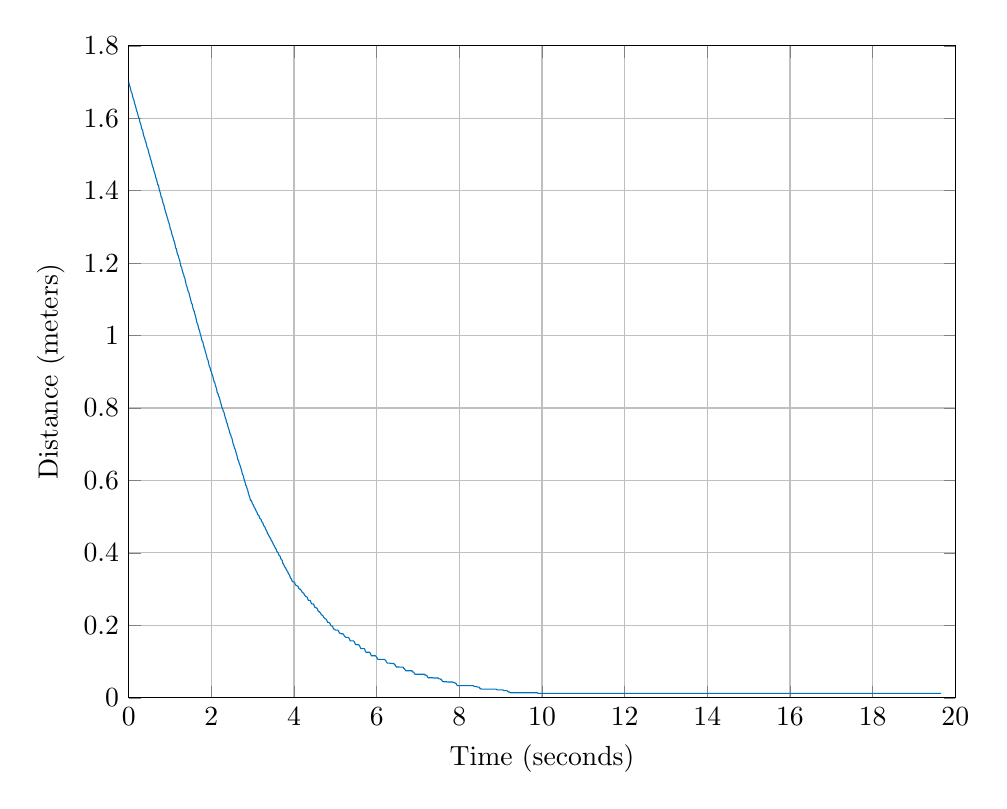
\begin{tikzpicture}

\begin{axis}[%
width=4.133in,
height=3.26in,
at={(0.693in,0.44in)},
scale only axis,
xmin=0,
xmax=20,
xmajorgrids,
xlabel={Time (seconds)},
ymin=0,
ymax=1.8,
ymajorgrids,
ylabel={Distance (meters)},
axis background/.style={fill=white}
]
\addplot [color=mycolor1,solid,forget plot]
  table[row sep=crcr]{%
0	1.70070346345311\\
0.0159777239999995	1.69086623549288\\
0.0321090869999975	1.68694606942081\\
0.0481079189999998	1.67910814535925\\
0.0640590819999985	1.67126980358659\\
0.0800937399999984	1.66931025400019\\
0.0961115539999977	1.65951269215463\\
0.112059099999998	1.65363385007974\\
0.128095164999999	1.64931765844527\\
0.144107822999999	1.63987454174872\\
0.16022602	1.63595492795775\\
0.176436053999998	1.62811765642852\\
0.192274968999997	1.62028010937229\\
0.208312000999998	1.61636077546817\\
0.224445437998999	1.60852406538375\\
0.240256767999999	1.60264594927523\\
0.256235530999999	1.59832898334341\\
0.272246213999998	1.58888312619996\\
0.288256415999997	1.58496382814955\\
0.304284272999998	1.57712743782508\\
0.320100665999997	1.56929053311861\\
0.336138408999998	1.56733139961559\\
0.352117502	1.55753558024245\\
0.368261987999998	1.54969907825446\\
0.384245494999997	1.54613077989034\\
0.400415454	1.53789213540846\\
0.416190528999999	1.53397324077266\\
0.432241748999998	1.52613738235538\\
0.448555228	1.51830131681099\\
0.464279937998999	1.51634227443859\\
0.480295162	1.50654744408871\\
0.49611382	1.5006704266809\\
0.512098092999998	1.49514035442108\\
0.528080552999999	1.48690123397875\\
0.544258044	1.48298268579319\\
0.560240717999998	1.47514768322867\\
0.576125136	1.46731231043609\\
0.592136877	1.46339418756768\\
0.608087463000998	1.45555948716013\\
0.624155911998998	1.44968297377696\\
0.640162150999997	1.44414956916429\\
0.656130693	1.435910793922\\
0.67221327	1.43199260880842\\
0.68816977	1.42415826163431\\
0.704135465999998	1.41632363508731\\
0.720146831	1.41436497297949\\
0.736124138999999	1.40457209797902\\
0.752133623999998	1.39829014301762\\
0.768111457999997	1.39275499500338\\
0.784161891999997	1.38296187724803\\
0.800203063999999	1.38100274330014\\
0.815989068	1.37316918514025\\
0.832085289999999	1.36533528603085\\
0.848108046	1.36141793146981\\
0.864191298	1.35358480038007\\
0.880130037999999	1.34608643900443\\
0.896134327	1.33980530655271\\
0.912191801999997	1.33393075027502\\
0.928191123999998	1.32805514303883\\
0.944326538999997	1.32218050962173\\
0.960005068999998	1.31434729718399\\
0.975954465999998	1.31043030750969\\
0.994062927999999	1.30259820302532\\
1.008973902	1.29273261691757\\
1.024018673	1.29077421622775\\
1.04210057	1.28098296194298\\
1.057133716	1.27510805200319\\
1.072491786	1.27119213207775\\
1.088189691	1.26335984388454\\
1.104071191	1.25944315419837\\
1.12011525	1.25161148210253\\
1.136083732	1.24174254875148\\
1.152086726001	1.23978431349393\\
1.168159963	1.2299941425369\\
1.18416712	1.224119721145\\
1.200112557	1.22020432742915\\
1.216133777	1.21237260627333\\
1.232151	1.20845649472547\\
1.248162628	1.19939812090512\\
1.264100654	1.19075307292089\\
1.280134106	1.18879499203392\\
1.296260263	1.17900576464386\\
1.312368036	1.17313192052206\\
1.328273386	1.16921675702218\\
1.344277093	1.16138619879248\\
1.360264749	1.1574700887325\\
1.376308177	1.14800392007756\\
1.392147707	1.13976389243298\\
1.408238111	1.13584790561907\\
1.424364075	1.12801779537965\\
1.440368358999	1.12214464641739\\
1.45627411	1.11822994905229\\
1.472293187	1.11039970156443\\
1.488109279	1.10370422446892\\
1.504243933	1.09660546439822\\
1.520258225	1.0887753081103\\
1.536146811	1.0868177745682\\
1.55208722	1.07703046466286\\
1.568197089	1.07115775969259\\
1.584110902	1.06724357385537\\
1.600089497999	1.05941436547601\\
1.616132715	1.05426413414225\\
1.632093845	1.04561666651659\\
1.648256884	1.03582997647433\\
1.664125781	1.03387267106571\\
1.680166707999	1.02604345271057\\
1.696118547	1.01821439636613\\
1.712264117	1.01430054346054\\
1.728294474	1.00564679555746\\
1.744231731	1.00049942572653\\
1.760298086	0.992671247962231\\
1.776224423	0.984842604006746\\
1.792030927	0.982885537825442\\
1.807977945	0.975057419161353\\
1.824104358	0.967228630175049\\
1.84015205	0.963315275071055\\
1.856144402	0.954247590731266\\
1.872143137	0.949511238610434\\
1.888269326999	0.941683749932993\\
1.904259434	0.933856074035005\\
1.920210107	0.931899128073447\\
1.936167358001	0.922114519337754\\
1.953769552	0.914287764321305\\
1.968766098	0.911917798954209\\
1.984172512	0.902848300216701\\
2.000055557	0.900480960564186\\
2.016107328	0.892653756780975\\
2.032082961	0.888739577896366\\
2.047948488	0.880913274758025\\
2.064123039	0.873086674282498\\
2.080253094	0.871129944704542\\
2.096106396	0.862890028866156\\
2.112099098	0.857731258489418\\
2.128102315	0.851450482460543\\
2.144102394	0.841667331314645\\
2.160072154	0.839710971400591\\
2.176111929	0.831884634581978\\
2.192199842	0.829928337107122\\
2.208235672	0.822102820506799\\
2.22406288	0.814276337703998\\
2.240190417	0.808702066723569\\
2.256381073	0.800463858163385\\
2.272243385	0.798507417931363\\
2.288173135	0.790681723470003\\
2.304232829	0.788725835021385\\
2.320228102999	0.780900367313005\\
2.33633977	0.773074463440338\\
2.352253288	0.769162924516195\\
2.368221054	0.760087812582637\\
2.384249517	0.75771603544379\\
2.40028206	0.74947795513265\\
2.416263878	0.743609588276014\\
2.432302685	0.737740778196293\\
2.448240964	0.729916319128132\\
2.464114858	0.727960841427103\\
2.480115784	0.720136244974353\\
2.496100107	0.716927748025705\\
2.512297197	0.708687234809073\\
2.528419017	0.700448375623395\\
2.544588425	0.696536864507616\\
2.56024656	0.688713262554401\\
2.576245436	0.686757258129132\\
2.592238885	0.678933453940243\\
2.608111827	0.673066899952459\\
2.624051364	0.665943299117577\\
2.640230033	0.657702387033726\\
2.656347784	0.655332088201222\\
2.672496138	0.647508656759513\\
2.688116818	0.643596866497596\\
2.704089786	0.637730019368293\\
2.720099818001	0.631863276628232\\
2.736095838	0.625995776470785\\
2.752089863	0.616915694638346\\
2.768088439	0.614541859925255\\
2.78412451	0.606303189037359\\
2.800109725	0.600436414331393\\
2.816095106	0.594569931012739\\
2.832099886	0.586747375831654\\
2.848126155	0.584792259096338\\
2.864113966	0.576970888468795\\
2.880085315	0.573754539108983\\
2.896158973	0.563558302236105\\
2.912117762	0.559230943131185\\
2.928091967	0.553364319830028\\
2.946335038	0.54554235001415\\
2.960220531999	0.545542626862491\\
2.975997723	0.541631860275187\\
2.994035466	0.535765237390957\\
3.008886524	0.533809744117906\\
3.023980285	0.529898904330135\\
3.040050652	0.524725700020631\\
3.058409402	0.522350969621772\\
3.073724191	0.518440129834001\\
3.089057911	0.514529073423288\\
3.104220408	0.512156732511877\\
3.120129546	0.506290913522093\\
3.136087775	0.504334836313393\\
3.152204474	0.502379343040342\\
3.168175214	0.496513524050558\\
3.184063869	0.494557446841859\\
3.200324903	0.492601953568808\\
3.216389118	0.486736134579024\\
3.232121376	0.484780057370324\\
3.248099049	0.482402596895119\\
3.264245274	0.475696597208698\\
3.280228671	0.47332128287419\\
3.296186249	0.47136578960114\\
3.31226691	0.465499970611355\\
3.328344535	0.463127045764295\\
3.344470665	0.459216279176991\\
3.360073559	0.453349656292761\\
3.376284316	0.45139416301971\\
3.392086220999	0.447483323231939\\
3.408085408	0.443572266821226\\
3.424105297	0.441616773548175\\
3.440095219	0.437705933760405\\
3.456060304	0.433372910147537\\
3.474233666	0.430577236177849\\
3.48923155	0.426247159264271\\
3.50429394	0.422336102853558\\
3.520112883	0.420380609580507\\
3.536269312001	0.416052922154376\\
3.552108657	0.412141865743663\\
3.568248563	0.410186372470612\\
3.584194204	0.404320553480828\\
3.600108905	0.402364476272128\\
3.616185723	0.400408982999077\\
3.632097821	0.394543164009293\\
3.648037896	0.392587086800594\\
3.664125245	0.390631593527543\\
3.679971729	0.383923205069124\\
3.698163256	0.381547549430267\\
3.713224225	0.379172819031409\\
3.728268674	0.371350922832925\\
3.744603386	0.369395429559874\\
3.760268757	0.365067742133743\\
3.776252349	0.36115668572303\\
3.792154195	0.359201192449979\\
3.808297753999	0.355290352662208\\
3.824360982	0.351379296251495\\
3.840176183	0.349423802978445\\
3.856079076999	0.345512963190674\\
3.872079837	0.341601906779961\\
3.88809921	0.339224446304756\\
3.90416367	0.334473425820348\\
3.920101959	0.330143132283827\\
3.936103893	0.328187639010777\\
3.953505749	0.322321820020992\\
3.968727644	0.320365742812293\\
3.984195998	0.319948895173932\\
4.000113279999	0.319948895173932\\
4.016112503	0.317993401900881\\
4.032108232001	0.312127582911097\\
4.048112469	0.310171505702398\\
4.064017835	0.310171505702398\\
4.080125713001	0.308216012429347\\
4.096168279	0.308216012429347\\
4.112117368	0.302350193439562\\
4.128101065	0.300394116230863\\
4.144104746999	0.300394116230863\\
4.16009529	0.298438622957813\\
4.176244918	0.296483056484296\\
4.192233922	0.292572803968028\\
4.208116128999	0.290194759557174\\
4.224219618	0.289774157290695\\
4.24030085	0.287399085587486\\
4.256306613	0.283069008673908\\
4.272276609	0.281114029471894\\
4.288177348	0.279157952263195\\
4.304241251	0.279157952263195\\
4.320323251	0.277202458990144\\
4.336301852	0.27133664000036\\
4.352112322	0.2689637151533\\
4.368048416	0.2689637151533\\
4.384087213	0.2689637151533\\
4.400094954	0.267008221880249\\
4.416085697	0.261142402890465\\
4.432098616	0.259186325681765\\
4.448237735	0.259186325681765\\
4.464175503	0.259186325681765\\
4.480095395	0.257230832408714\\
4.496126529999	0.25136501341893\\
4.512102179	0.249408936210231\\
4.528148673	0.249408936210231\\
4.543985698	0.24745344293718\\
4.559953039	0.247031475735025\\
4.575984265	0.241165656745241\\
4.591962851	0.238369398839904\\
4.608247046	0.238369398839904\\
4.624348931	0.235994668441046\\
4.640116824	0.234039101967529\\
4.656129131	0.230128849451261\\
4.672087406	0.228172772242562\\
4.688260842	0.228172772242562\\
4.704292027	0.225800431331151\\
4.72024058	0.22188959154338\\
4.736289364	0.219934612341366\\
4.752277877	0.217978535132667\\
4.768277055	0.217978535132667\\
4.784291445999	0.216023041859616\\
4.800018635	0.212112202071845\\
4.816296806	0.208201145661133\\
4.832195334	0.208201145661133\\
4.848246475	0.208201145661133\\
4.864267708	0.206245652388082\\
4.880089121999	0.202334812600311\\
4.896055935	0.198423756189598\\
4.912233101	0.198423756189598\\
4.928344237	0.198001788987443\\
4.944393427	0.193670126974396\\
4.961718553	0.189759874458129\\
4.976874884001	0.189340296027971\\
4.992295793	0.187384218819272\\
5.008099858001	0.186964981693464\\
5.024087354	0.186964981693464\\
5.040159537	0.186964981693464\\
5.056114068	0.186964981693464\\
5.072159344	0.185009488420413\\
5.088159469	0.181098648632643\\
5.104143301	0.179143669430629\\
5.120154876	0.17718759222193\\
5.136144642	0.17718759222193\\
5.152101103	0.176770744583569\\
5.168098661	0.176770744583569\\
5.184127656	0.176770744583569\\
5.200091984	0.174815251310518\\
5.216077023999	0.170904411522747\\
5.232104464999	0.168949432320734\\
5.250590581	0.166993355112034\\
5.265640408	0.166993355112034\\
5.280804437999	0.166993355112034\\
5.296168947	0.166993355112034\\
5.312194178	0.166993355112034\\
5.328174543	0.165037861838984\\
5.344271256	0.161127022051213\\
5.360290408	0.1572159656405\\
5.3762937	0.1572159656405\\
5.39225227	0.1572159656405\\
5.408216699	0.1572159656405\\
5.424320493	0.1572159656405\\
5.440259554	0.1572159656405\\
5.456272963001	0.155260472367449\\
5.472278355	0.151349632579679\\
5.488316941	0.147016608966811\\
5.50446695	0.147016608966811\\
5.5202356	0.147016608966811\\
5.536191975	0.146596006700331\\
5.552063889	0.146596006700331\\
5.568096858	0.146176428270174\\
5.584095901	0.144220934997123\\
5.600086046	0.139890858083545\\
5.616145284001	0.135979801672832\\
5.632130981	0.135979801672832\\
5.648264167	0.135979801672832\\
5.664117593	0.135979801672832\\
5.680122785	0.135979801672832\\
5.696124557	0.135979801672832\\
5.712126857	0.134024308399781\\
5.728099599	0.12774054376495\\
5.744203408	0.125785564562936\\
5.760259259	0.125785564562936\\
5.776226444	0.125785564562936\\
5.792139841	0.125785564562936\\
5.80810212	0.125785564562936\\
5.824077478	0.125785564562936\\
5.840078048001	0.123830071289886\\
5.856066896	0.119918427607669\\
5.872029642	0.116008175091402\\
5.888096402	0.116008175091402\\
5.904377142	0.116008175091402\\
5.920268064	0.116008175091402\\
5.936240811	0.116008175091402\\
5.95416099	0.116008175091402\\
5.969498242	0.116008175091402\\
5.985008788	0.114052681818351\\
6.000421863	0.112096604609651\\
6.016104768	0.108185764821881\\
6.032255534	0.106230785619867\\
6.048244167	0.106230785619867\\
6.064238358	0.106230785619867\\
6.080274393	0.106230785619867\\
6.096286184	0.106230785619867\\
6.112102527	0.106230785619867\\
6.128365231	0.106230785619867\\
6.144091896001	0.106230785619867\\
6.160252649	0.106230785619867\\
6.176303499	0.106230785619867\\
6.192278717	0.105808818417713\\
6.208381203	0.103853325144662\\
6.224280313	0.101897247935963\\
6.240256969	0.0979864081481916\\
6.256243878	0.0960314289461781\\
6.272113878	0.0956108266796987\\
6.288178428	0.0956108266796987\\
6.304001469	0.0956108266796987\\
6.320088728	0.0956108266796987\\
6.336314454	0.0951912482495412\\
6.3522912	0.0951912482495412\\
6.368237462	0.0951912482495412\\
6.384265349	0.0947720111237333\\
6.400370241	0.0947720111237333\\
6.416093924	0.0947720111237333\\
6.4320925	0.0908604406419835\\
6.448241932	0.0908604406419835\\
6.464177155	0.0869496008542123\\
6.480089931	0.0849946216521988\\
6.496066983	0.0849946216521988\\
6.51211214	0.0849946216521988\\
6.528241467	0.0849946216521988\\
6.544276731	0.0849946216521988\\
6.560089761	0.084577774013838\\
6.576070131	0.084577774013838\\
6.592084267	0.084577774013838\\
6.608270642999	0.084577774013838\\
6.624230215	0.084577774013838\\
6.640371233999	0.084577774013838\\
6.656293918	0.080666203532088\\
6.672419566	0.080666203532088\\
6.688118042001	0.076755363744317\\
6.704094548	0.0748003845423035\\
6.720247910001	0.0748003845423035\\
6.736293216	0.0748003845423035\\
6.752118665	0.0748003845423035\\
6.768093898	0.0748003845423035\\
6.784105829	0.0748003845423035\\
6.800233983	0.0748003845423035\\
6.816268505	0.0748003845423035\\
6.83221159	0.0748003845423035\\
6.848086276	0.0748003845423035\\
6.864117094	0.0728443073336045\\
6.880269113	0.0708888140605537\\
6.896338679	0.0708888140605537\\
6.912140459	0.066977974272783\\
6.928093727	0.0650229950707693\\
6.944177697	0.0650229950707693\\
6.961630842	0.0650229950707693\\
6.976705595	0.0650229950707693\\
6.992307027	0.0650229950707693\\
7.008268574	0.0650229950707693\\
7.024037568	0.0650229950707693\\
7.040151211	0.0650229950707693\\
7.056142565	0.0650229950707693\\
7.072270509	0.0650229950707693\\
7.088155834	0.0650229950707693\\
7.104108906	0.0650229950707693\\
7.120224317	0.0650229950707693\\
7.136114783	0.0650229950707693\\
7.152237389	0.0650229950707693\\
7.168329688	0.06306691786207\\
7.18434001	0.06306691786207\\
7.200266803	0.0611114245890192\\
7.216262993	0.0611114245890192\\
7.232028907	0.0572005848012482\\
7.250248364	0.0552456055992347\\
7.265570975001	0.0552456055992347\\
7.281339102	0.0552456055992347\\
7.297183113	0.0552456055992347\\
7.312662167	0.0552456055992347\\
7.328281403	0.0552456055992347\\
7.344266809	0.0552456055992347\\
7.360272481	0.0552456055992347\\
7.37625896	0.0548236383970802\\
7.392298874	0.0548236383970802\\
7.408251335	0.0548236383970802\\
7.424108556	0.0548236383970802\\
7.440263530999	0.0548236383970802\\
7.456209778	0.0548236383970802\\
7.472318323	0.0548236383970802\\
7.488248474	0.0548236383970802\\
7.504262675	0.0524469589219017\\
7.520283463	0.0524469589219017\\
7.536179692001	0.0524469589219017\\
7.552479413	0.0504914656488509\\
7.568254261999	0.0504914656488509\\
7.58438835	0.0465806258610799\\
7.600412131	0.0446256466590664\\
7.616258714	0.0446256466590664\\
7.632253231	0.0442060682289087\\
7.64828426	0.0442060682289087\\
7.664125595	0.0442060682289087\\
7.680164306	0.0442060682289087\\
7.696105487	0.0442060682289087\\
7.712163162	0.0437868311031009\\
7.728110132	0.0437868311031009\\
7.744049321	0.0437868311031009\\
7.760126581	0.0437868311031009\\
7.776148991	0.0437868311031009\\
7.792165743	0.0437868311031009\\
7.808046159	0.0437868311031009\\
7.824043769	0.0437868311031009\\
7.840093306	0.0437868311031009\\
7.856154118	0.0418307538944016\\
7.872132398	0.0418307538944016\\
7.888141176	0.0418307538944016\\
7.904200374	0.0398752606213508\\
7.920136604	0.0398752606213508\\
7.93615076	0.0359644208335801\\
7.953456651	0.0335925939932056\\
7.968391552	0.0335925939932056\\
7.98406813	0.0335925939932056\\
8.000115071	0.0335925939932056\\
8.016118283	0.0335925939932056\\
8.032268877	0.0335925939932056\\
8.048431685	0.0335925939932056\\
8.064168181999	0.0335925939932056\\
8.080184618	0.0335925939932056\\
8.096195196	0.0335925939932056\\
8.11215072	0.0335925939932056\\
8.128133088	0.0335925939932056\\
8.144044822	0.0335925939932056\\
8.160124317	0.0335925939932056\\
8.176154679	0.0335925939932056\\
8.192137891	0.0335925939932056\\
8.208157659	0.0335925939932056\\
8.224159458	0.0335925939932056\\
8.240219558	0.0335925939932056\\
8.256082652	0.0335925939932056\\
8.27199661	0.0335925939932056\\
8.288092987	0.0335925939932056\\
8.304190633	0.0335925939932056\\
8.320243181	0.0335925939932056\\
8.336155421	0.0335925939932056\\
8.352194193	0.0316365167845065\\
8.368273070999	0.0316365167845065\\
8.384222294999	0.0316365167845065\\
8.400181346	0.0316365167845065\\
8.416134484	0.0316365167845065\\
8.432155631	0.029681023511456\\
8.448128193	0.029681023511456\\
8.464156606	0.029681023511456\\
8.480154003999	0.029681023511456\\
8.496266208	0.025770183723685\\
8.512111431	0.025770183723685\\
8.528266647	0.0238152045216715\\
8.544314674	0.0238152045216715\\
8.560297364	0.0238152045216715\\
8.576287867	0.0238152045216715\\
8.592279036	0.0238152045216715\\
8.608080370001	0.0238152045216715\\
8.624265032	0.0238152045216715\\
8.640275169	0.0238152045216715\\
8.656299218001	0.0238152045216715\\
8.672308287	0.0238152045216715\\
8.688181579	0.0238152045216715\\
8.704377006	0.0238152045216715\\
8.720117572	0.0238152045216715\\
8.736222895	0.0238152045216715\\
8.752169197	0.0238152045216715\\
8.768185725	0.0238152045216715\\
8.784069627	0.0238152045216715\\
8.800054688	0.0238152045216715\\
8.816013448	0.0238152045216715\\
8.832268046	0.0238152045216715\\
8.848122862	0.0238152045216715\\
8.864161333	0.0238152045216715\\
8.880146012	0.0238152045216715\\
8.896107219	0.0238152045216715\\
8.91218809	0.021859127312972\\
8.928099663	0.021859127312972\\
8.944129055	0.021859127312972\\
8.960250881	0.021859127312972\\
8.976348519	0.021859127312972\\
8.992208452	0.021859127312972\\
9.008062036	0.021859127312972\\
9.024159369	0.021859127312972\\
9.040162043	0.021859127312972\\
9.056263187	0.021859127312972\\
9.072157797	0.0199036340399212\\
9.088168295	0.0199036340399212\\
9.104227889	0.0199036340399212\\
9.120096475	0.0199036340399212\\
9.136108015	0.0199036340399212\\
9.152090525	0.0199036340399212\\
9.168090724	0.0179483607256676\\
9.184097148	0.0159927942521505\\
9.20007414	0.0159927942521505\\
9.21610561	0.0159927942521505\\
9.232149016999	0.0140378150501368\\
9.248159686	0.0140378150501368\\
9.26415994	0.0140378150501368\\
9.280191446	0.0140378150501368\\
9.296171354	0.0140378150501368\\
9.312116955	0.0140378150501368\\
9.328143584	0.0140378150501368\\
9.344119379	0.0140378150501368\\
9.360432813	0.0140378150501368\\
9.376183412	0.0140378150501368\\
9.39215687	0.0140378150501368\\
9.408143063	0.0140378150501368\\
9.424167718	0.0140378150501368\\
9.440152462	0.0140378150501368\\
9.456159047	0.0140378150501368\\
9.472144502	0.0140378150501368\\
9.488135505	0.0140378150501368\\
9.50412233	0.0140378150501368\\
9.520103447	0.0140378150501368\\
9.536119412	0.0140378150501368\\
9.552133588	0.0140378150501368\\
9.568055895	0.0140378150501368\\
9.584151442	0.0140378150501368\\
9.600121172	0.0140378150501368\\
9.616112997	0.0140378150501368\\
9.632090316	0.0140378150501368\\
9.648149257	0.0140378150501368\\
9.664049222	0.0140378150501368\\
9.680137715	0.0140378150501368\\
9.696147085	0.0140378150501368\\
9.712129058	0.0140378150501368\\
9.728254772001	0.0140378150501368\\
9.744174063	0.0140378150501368\\
9.760166304	0.0140378150501368\\
9.776138942	0.0140378150501368\\
9.792132992	0.0140378150501368\\
9.808182198	0.0140378150501368\\
9.824162758	0.0140378150501368\\
9.84018215	0.0140378150501368\\
9.856214974	0.0140378150501368\\
9.872098304	0.0140378150501368\\
9.888116734	0.0140378150501368\\
9.904078161	0.0120817378414375\\
9.920110408	0.0120817378414375\\
9.936068382	0.0120817378414375\\
9.954008335	0.0120817378414375\\
9.969494926	0.0120817378414375\\
9.984763203	0.0120817378414375\\
10.0001576	0.0120817378414375\\
10.016058485	0.0120817378414375\\
10.032128507	0.0120817378414375\\
10.048063225	0.0120817378414375\\
10.066290568	0.0120817378414375\\
10.081778016001	0.0120817378414375\\
10.097111305	0.0120817378414375\\
10.112814496	0.0120817378414375\\
10.128169745	0.0120817378414375\\
10.144215469	0.0120817378414375\\
10.160370402	0.0120817378414375\\
10.176183628	0.0120817378414375\\
10.192149372	0.0120817378414375\\
10.208330033	0.0120817378414375\\
10.224134609	0.0120817378414375\\
10.240122225	0.0120817378414375\\
10.256418165	0.0120817378414375\\
10.272231312999	0.0120817378414375\\
10.288143616	0.0120817378414375\\
10.304347546	0.0120817378414375\\
10.320193747	0.0120817378414375\\
10.336127157	0.0120817378414375\\
10.352138379999	0.0120817378414375\\
10.368185187001	0.0120817378414375\\
10.38418979	0.0120817378414375\\
10.400215311	0.0120817378414375\\
10.416189903	0.0120817378414375\\
10.432085871	0.0120817378414375\\
10.448100393	0.0120817378414375\\
10.464160708999	0.0120817378414375\\
10.480122927	0.0120817378414375\\
10.496115554	0.0120817378414375\\
10.512099167	0.0120817378414375\\
10.528102749	0.0120817378414375\\
10.544173107	0.0120817378414375\\
10.560101744	0.0120817378414375\\
10.576041276	0.0120817378414375\\
10.592229812999	0.0120817378414375\\
10.60840134	0.0120817378414375\\
10.624268338001	0.0120817378414375\\
10.640122747	0.0120817378414375\\
10.656125377001	0.0120817378414375\\
10.672257199	0.0120817378414375\\
10.68836583	0.0120817378414375\\
10.704248347	0.0120817378414375\\
10.720252962	0.0120817378414375\\
10.736536043	0.0120817378414375\\
10.752283439	0.0120817378414375\\
10.768305393	0.0120817378414375\\
10.784119406	0.0120817378414375\\
10.800050331	0.0120817378414375\\
10.816099163	0.0120817378414375\\
10.832273111	0.0120817378414375\\
10.84826898	0.0120817378414375\\
10.8641012	0.0120817378414375\\
10.880083668999	0.0120817378414375\\
10.89609571	0.0120817378414375\\
10.912121723	0.0120817378414375\\
10.928229590999	0.0120817378414375\\
10.944229104	0.0120817378414375\\
10.961943987	0.0120817378414375\\
10.978185314	0.0120817378414375\\
10.993472378	0.0120817378414375\\
11.009054404999	0.0120817378414375\\
11.024576592	0.0120817378414375\\
11.040438137	0.0120817378414375\\
11.056240083	0.0120817378414375\\
11.072238448	0.0120817378414375\\
11.088084047	0.0120817378414375\\
11.104279338	0.0120817378414375\\
11.14056567	0.0120817378414375\\
11.156090263	0.0120817378414375\\
11.174180867	0.0120817378414375\\
11.189216217	0.0120817378414375\\
11.204138304	0.0120817378414375\\
11.220094718	0.0120817378414375\\
11.236247585	0.0120817378414375\\
11.252081463	0.0120817378414375\\
11.268131472	0.0120817378414375\\
11.284185857	0.0120817378414375\\
11.301197757	0.0120817378414375\\
11.31617367	0.0120817378414375\\
11.332097319	0.0120817378414375\\
11.348133169	0.0120817378414375\\
11.364154925	0.0120817378414375\\
11.38018726	0.0120817378414375\\
11.396321416	0.0120817378414375\\
11.41247177	0.0120817378414375\\
11.428266431	0.0120817378414375\\
11.444498516	0.0120817378414375\\
11.460372850001	0.0120817378414375\\
11.476181217	0.0120817378414375\\
11.492497469	0.0120817378414375\\
11.50833055	0.0120817378414375\\
11.524244565	0.0120817378414375\\
11.540323808	0.0120817378414375\\
11.556233861	0.0120817378414375\\
11.57227684	0.0120817378414375\\
11.588206124	0.0120817378414375\\
11.604147515	0.0120817378414375\\
11.622519212	0.0120817378414375\\
11.637746065	0.0120817378414375\\
11.653107362	0.0120817378414375\\
11.668552499	0.0120817378414375\\
11.684533377	0.0120817378414375\\
11.700522194	0.0120817378414375\\
11.716316141	0.0120817378414375\\
11.732343737	0.0120817378414375\\
11.748186825001	0.0120817378414375\\
11.764164739	0.0120817378414375\\
11.78269695	0.0120817378414375\\
11.797938659	0.0120817378414375\\
11.813895397	0.0120817378414375\\
11.829170168	0.0120817378414375\\
11.844443805	0.0120817378414375\\
11.86017635	0.0120817378414375\\
11.876329752	0.0120817378414375\\
11.892193963	0.0120817378414375\\
11.908258539	0.0120817378414375\\
11.924289037	0.0120817378414375\\
11.940230408	0.0120817378414375\\
11.957686646	0.0120817378414375\\
11.972635829	0.0120817378414375\\
11.988202807	0.0120817378414375\\
12.004110929	0.0120817378414375\\
12.020174541	0.0120817378414375\\
12.036210823	0.0120817378414375\\
12.052244197	0.0120817378414375\\
12.068197732	0.0120817378414375\\
12.084263905	0.0120817378414375\\
12.100114284	0.0120817378414375\\
12.118373416	0.0120817378414375\\
12.133537372	0.0120817378414375\\
12.148756377001	0.0120817378414375\\
12.164161323	0.0120817378414375\\
12.180420499	0.0120817378414375\\
12.196166312	0.0120817378414375\\
12.212328503999	0.0120817378414375\\
12.228268632	0.0120817378414375\\
12.244299015	0.0120817378414375\\
12.260200494	0.0120817378414375\\
12.276425173	0.0120817378414375\\
12.292235112	0.0120817378414375\\
12.308182512	0.0120817378414375\\
12.32422837	0.0120817378414375\\
12.340138043	0.0120817378414375\\
12.356086801	0.0120817378414375\\
12.372273815	0.0120817378414375\\
12.388308718	0.0120817378414375\\
12.416152325	0.0120817378414375\\
12.421598838	0.0120817378414375\\
12.436787575	0.0120817378414375\\
12.452107865	0.0120817378414375\\
12.470407512	0.0120817378414375\\
12.485587789	0.0120817378414375\\
12.500756035	0.0120817378414375\\
12.51622933	0.0120817378414375\\
12.532286183	0.0120817378414375\\
12.550672483	0.0120817378414375\\
12.565836232	0.0120817378414375\\
12.581019766999	0.0120817378414375\\
12.596378906	0.0120817378414375\\
12.612486994	0.0120817378414375\\
12.628237858	0.0120817378414375\\
12.644281656	0.0120817378414375\\
12.660331654	0.0120817378414375\\
12.676280739	0.0120817378414375\\
12.703150408	0.0120817378414375\\
12.708526156	0.0120817378414375\\
12.724101477	0.0120817378414375\\
12.740080173	0.0120817378414375\\
12.756338874	0.0120817378414375\\
12.77223381	0.0120817378414375\\
12.78832044	0.0120817378414375\\
12.80429664	0.0120817378414375\\
12.820262221	0.0120817378414375\\
12.836253291	0.0120817378414375\\
12.852412891	0.0120817378414375\\
12.868279262	0.0120817378414375\\
12.884276705	0.0120817378414375\\
12.900277666	0.0120817378414375\\
12.916333154	0.0120817378414375\\
12.932280902	0.0120817378414375\\
12.951023434	0.0120817378414375\\
12.964155696	0.0120817378414375\\
12.98013903	0.0120817378414375\\
12.996303048	0.0120817378414375\\
13.012175142	0.0120817378414375\\
13.028327885	0.0120817378414375\\
13.044290782	0.0120817378414375\\
13.060159394	0.0120817378414375\\
13.076308029	0.0120817378414375\\
13.092347969	0.0120817378414375\\
13.108220809	0.0120817378414375\\
13.124361052	0.0120817378414375\\
13.140234409	0.0120817378414375\\
13.156290234	0.0120817378414375\\
13.172214176	0.0120817378414375\\
13.188287306	0.0120817378414375\\
13.204185253	0.0120817378414375\\
13.220255281	0.0120817378414375\\
13.236193671	0.0120817378414375\\
13.252252323	0.0120817378414375\\
13.268258636	0.0120817378414375\\
13.284257182	0.0120817378414375\\
13.300331759	0.0120817378414375\\
13.316196617	0.0120817378414375\\
13.332258822	0.0120817378414375\\
13.348353904	0.0120817378414375\\
13.364175872	0.0120817378414375\\
13.38025882	0.0120817378414375\\
13.396199319	0.0120817378414375\\
13.41227738	0.0120817378414375\\
13.428234832999	0.0120817378414375\\
13.444295348	0.0120817378414375\\
13.460343276	0.0120817378414375\\
13.476438550999	0.0120817378414375\\
13.492245452	0.0120817378414375\\
13.50816392	0.0120817378414375\\
13.524122177	0.0120817378414375\\
13.540228055001	0.0120817378414375\\
13.556316334	0.0120817378414375\\
13.572316589	0.0120817378414375\\
13.588250618	0.0120817378414375\\
13.604291983001	0.0120817378414375\\
13.620190097	0.0120817378414375\\
13.6361217	0.0120817378414375\\
13.652272262	0.0120817378414375\\
13.668281894	0.0120817378414375\\
13.684268355	0.0120817378414375\\
13.700246159	0.0120817378414375\\
13.716207568	0.0120817378414375\\
13.732278833999	0.0120817378414375\\
13.748399904001	0.0120817378414375\\
13.764214546	0.0120817378414375\\
13.780229037	0.0120817378414375\\
13.796274304	0.0120817378414375\\
13.812579755	0.0120817378414375\\
13.828640161	0.0120817378414375\\
13.844227883	0.0120817378414375\\
13.860539406	0.0120817378414375\\
13.876630882	0.0120817378414375\\
13.892161578	0.0120817378414375\\
13.908248429	0.0120817378414375\\
13.924139106	0.0120817378414375\\
13.94022758	0.0120817378414375\\
13.958053117	0.0120817378414375\\
13.972995582	0.0120817378414375\\
13.988124967	0.0120817378414375\\
14.006194018	0.0120817378414375\\
14.021187427	0.0120817378414375\\
14.036132207999	0.0120817378414375\\
14.052262677	0.0120817378414375\\
14.068270574	0.0120817378414375\\
14.084324316	0.0120817378414375\\
14.100242004	0.0120817378414375\\
14.116124141	0.0120817378414375\\
14.132236188	0.0120817378414375\\
14.148514632	0.0120817378414375\\
14.164329497	0.0120817378414375\\
14.180282439	0.0120817378414375\\
14.196297292	0.0120817378414375\\
14.21225283	0.0120817378414375\\
14.228142407	0.0120817378414375\\
14.244184789	0.0120817378414375\\
14.26036428	0.0120817378414375\\
14.276303892	0.0120817378414375\\
14.292238047	0.0120817378414375\\
14.308275105	0.0120817378414375\\
14.324231906	0.0120817378414375\\
14.340255423001	0.0120817378414375\\
14.356290231	0.0120817378414375\\
14.372225053	0.0120817378414375\\
14.388090671	0.0120817378414375\\
14.404091663	0.0120817378414375\\
14.420078015	0.0120817378414375\\
14.436164222	0.0120817378414375\\
14.452075807999	0.0120817378414375\\
14.468313752001	0.0120817378414375\\
14.484543567	0.0120817378414375\\
14.500343447	0.0120817378414375\\
14.516236192	0.0120817378414375\\
14.532252285	0.0120817378414375\\
14.550682752	0.0120817378414375\\
14.564550373	0.0120817378414375\\
14.580319604	0.0120817378414375\\
14.596207800999	0.0120817378414375\\
14.612185558	0.0120817378414375\\
14.628232995	0.0120817378414375\\
14.644294259	0.0120817378414375\\
14.660120663	0.0120817378414375\\
14.676255578	0.0120817378414375\\
14.692271829	0.0120817378414375\\
14.708314019	0.0120817378414375\\
14.724199223	0.0120817378414375\\
14.740246108	0.0120817378414375\\
14.75630274	0.0120817378414375\\
14.77227455	0.0120817378414375\\
14.788313034	0.0120817378414375\\
14.804285669	0.0120817378414375\\
14.820375551	0.0120817378414375\\
14.83627178	0.0120817378414375\\
14.85218547	0.0120817378414375\\
14.868286826999	0.0120817378414375\\
14.884208337	0.0120817378414375\\
14.90033553	0.0120817378414375\\
14.916228612	0.0120817378414375\\
14.932255257	0.0120817378414375\\
14.953044645	0.0120817378414375\\
14.96482545	0.0120817378414375\\
14.980143421	0.0120817378414375\\
14.996097756	0.0120817378414375\\
15.01423209	0.0120817378414375\\
15.029268852	0.0120817378414375\\
15.044252895	0.0120817378414375\\
15.060202239	0.0120817378414375\\
15.076226613	0.0120817378414375\\
15.092176135	0.0120817378414375\\
15.108162427	0.0120817378414375\\
15.124364332	0.0120817378414375\\
15.140096146	0.0120817378414375\\
15.156291485	0.0120817378414375\\
15.172245811	0.0120817378414375\\
15.188173953	0.0120817378414375\\
15.204340934	0.0120817378414375\\
15.220095253	0.0120817378414375\\
15.238210708	0.0120817378414375\\
15.253333274	0.0120817378414375\\
15.268642744	0.0120817378414375\\
15.284201157	0.0120817378414375\\
15.30049381	0.0120817378414375\\
15.316306544	0.0120817378414375\\
15.332307305001	0.0120817378414375\\
15.348109325	0.0120817378414375\\
15.364111353	0.0120817378414375\\
15.380457477	0.0120817378414375\\
15.39628448	0.0120817378414375\\
15.412129321	0.0120817378414375\\
15.428196864	0.0120817378414375\\
15.444315452	0.0120817378414375\\
15.460265739001	0.0120817378414375\\
15.476253289	0.0120817378414375\\
15.492323703	0.0120817378414375\\
15.50812908	0.0120817378414375\\
15.524182221	0.0120817378414375\\
15.54008591	0.0120817378414375\\
15.556098878	0.0120817378414375\\
15.572264233	0.0120817378414375\\
15.588279411999	0.0120817378414375\\
15.604302207	0.0120817378414375\\
15.620271797	0.0120817378414375\\
15.636264475001	0.0120817378414375\\
15.652246573	0.0120817378414375\\
15.668276465	0.0120817378414375\\
15.684197117	0.0120817378414375\\
15.700285508	0.0120817378414375\\
15.716889881	0.0120817378414375\\
15.732216109	0.0120817378414375\\
15.748375434	0.0120817378414375\\
15.764282919	0.0120817378414375\\
15.780299148999	0.0120817378414375\\
15.796194646	0.0120817378414375\\
15.812341554	0.0120817378414375\\
15.828268913	0.0120817378414375\\
15.844289469001	0.0120817378414375\\
15.860223808	0.0120817378414375\\
15.876284766	0.0120817378414375\\
15.892257152001	0.0120817378414375\\
15.908444591	0.0120817378414375\\
15.924354357	0.0120817378414375\\
15.940240326	0.0120817378414375\\
15.957828668	0.0120817378414375\\
15.972815743	0.0120817378414375\\
15.988142807999	0.0120817378414375\\
16.006201298001	0.0120817378414375\\
16.021135685	0.0120817378414375\\
16.036148508	0.0120817378414375\\
16.052245953	0.0120817378414375\\
16.068270988	0.0120817378414375\\
16.084331602	0.0120817378414375\\
16.100333317	0.0120817378414375\\
16.116210332999	0.0120817378414375\\
16.132239308	0.0120817378414375\\
16.148543781	0.0120817378414375\\
16.164265931	0.0120817378414375\\
16.180324181999	0.0120817378414375\\
16.196204928	0.0120817378414375\\
16.212319239	0.0120817378414375\\
16.228195651	0.0120817378414375\\
16.24421434	0.0120817378414375\\
16.260441432	0.0120817378414375\\
16.276271848	0.0120817378414375\\
16.292262425	0.0120817378414375\\
16.308278842	0.0120817378414375\\
16.324271223	0.0120817378414375\\
16.34041397	0.0120817378414375\\
16.356299840999	0.0120817378414375\\
16.372287166	0.0120817378414375\\
16.388318973	0.0120817378414375\\
16.404333655	0.0120817378414375\\
16.420278509	0.0120817378414375\\
16.436177639	0.0120817378414375\\
16.452209525	0.0120817378414375\\
16.468215484999	0.0120817378414375\\
16.484138362	0.0120817378414375\\
16.500187832	0.0120817378414375\\
16.516194183	0.0120817378414375\\
16.532256823	0.0120817378414375\\
16.55074378	0.0120817378414375\\
16.565897152001	0.0120817378414375\\
16.581019001001	0.0120817378414375\\
16.596276569	0.0120817378414375\\
16.612288227	0.0120817378414375\\
16.628282114	0.0120817378414375\\
16.644285025	0.0120817378414375\\
16.66029454	0.0120817378414375\\
16.676269874	0.0120817378414375\\
16.692270469	0.0120817378414375\\
16.708322742	0.0120817378414375\\
16.724246535	0.0120817378414375\\
16.740262834	0.0120817378414375\\
16.756285134	0.0120817378414375\\
16.772271191	0.0120817378414375\\
16.788277369	0.0120817378414375\\
16.804235138	0.0120817378414375\\
16.820283556	0.0120817378414375\\
16.836267789	0.0120817378414375\\
16.852221047	0.0120817378414375\\
16.868287376	0.0120817378414375\\
16.884273484	0.0120817378414375\\
16.900344219001	0.0120817378414375\\
16.916230766	0.0120817378414375\\
16.932237665	0.0120817378414375\\
16.950719503	0.0120817378414375\\
16.965948426	0.0120817378414375\\
16.981222251	0.0120817378414375\\
16.996395298001	0.0120817378414375\\
17.01223971	0.0120817378414375\\
17.028223227	0.0120817378414375\\
17.044209444	0.0120817378414375\\
17.060232005	0.0120817378414375\\
17.076234549	0.0120817378414375\\
17.092245257	0.0120817378414375\\
17.108442754	0.0120817378414375\\
17.124253244	0.0120817378414375\\
17.140218845	0.0120817378414375\\
17.156278248	0.0120817378414375\\
17.17227295	0.0120817378414375\\
17.188298289	0.0120817378414375\\
17.204250218	0.0120817378414375\\
17.220274756	0.0120817378414375\\
17.23621662	0.0120817378414375\\
17.252282046	0.0120817378414375\\
17.268368882	0.0120817378414375\\
17.284252658	0.0120817378414375\\
17.300352954	0.0120817378414375\\
17.316279331	0.0120817378414375\\
17.332262777	0.0120817378414375\\
17.348250123	0.0120817378414375\\
17.364267361	0.0120817378414375\\
17.380333885999	0.0120817378414375\\
17.396273684	0.0120817378414375\\
17.412312781	0.0120817378414375\\
17.428266941	0.0120817378414375\\
17.444326265	0.0120817378414375\\
17.460334407	0.0120817378414375\\
17.476278454	0.0120817378414375\\
17.492360655	0.0120817378414375\\
17.508284325999	0.0120817378414375\\
17.524268162999	0.0120817378414375\\
17.540321107001	0.0120817378414375\\
17.556284358	0.0120817378414375\\
17.572271868	0.0120817378414375\\
17.588319987	0.0120817378414375\\
17.604261483	0.0120817378414375\\
17.620296692	0.0120817378414375\\
17.636232134	0.0120817378414375\\
17.652261771	0.0120817378414375\\
17.668308155	0.0120817378414375\\
17.684172168	0.0120817378414375\\
17.700343478	0.0120817378414375\\
17.716247074	0.0120817378414375\\
17.732256043	0.0120817378414375\\
17.750618333	0.0120817378414375\\
17.765867872	0.0120817378414375\\
17.781094103	0.0120817378414375\\
17.796344485	0.0120817378414375\\
17.812254856	0.0120817378414375\\
17.828165295	0.0120817378414375\\
17.844200946	0.0120817378414375\\
17.860142945	0.0120817378414375\\
17.876278134	0.0120817378414375\\
17.892296089	0.0120817378414375\\
17.90825522	0.0120817378414375\\
17.924223127	0.0120817378414375\\
17.940277246	0.0120817378414375\\
17.957852638	0.0120817378414375\\
17.972836437999	0.0120817378414375\\
17.988142337	0.0120817378414375\\
18.006234403	0.0120817378414375\\
18.021276106	0.0120817378414375\\
18.036463539	0.0120817378414375\\
18.052262082	0.0120817378414375\\
18.068293227	0.0120817378414375\\
18.084250385	0.0120817378414375\\
18.101171965	0.0120817378414375\\
18.116328283	0.0120817378414375\\
18.132266788	0.0120817378414375\\
18.148351063	0.0120817378414375\\
18.164278873	0.0120817378414375\\
18.18254261	0.0120817378414375\\
18.197660180001	0.0120817378414375\\
18.21274877	0.0120817378414375\\
18.228219515	0.0120817378414375\\
18.244212628999	0.0120817378414375\\
18.260159044	0.0120817378414375\\
18.276231143	0.0120817378414375\\
18.292220477999	0.0120817378414375\\
18.308276835	0.0120817378414375\\
18.324248791	0.0120817378414375\\
18.340272829	0.0120817378414375\\
18.356317003	0.0120817378414375\\
18.372178471	0.0120817378414375\\
18.388307053	0.0120817378414375\\
18.404259455	0.0120817378414375\\
18.420311146	0.0120817378414375\\
18.436235168	0.0120817378414375\\
18.452250902	0.0120817378414375\\
18.468277742	0.0120817378414375\\
18.484240131	0.0120817378414375\\
18.5027387	0.0120817378414375\\
18.518032594	0.0120817378414375\\
18.533480453	0.0120817378414375\\
18.548763884	0.0120817378414375\\
18.564309458	0.0120817378414375\\
18.580230644	0.0120817378414375\\
18.596282569999	0.0120817378414375\\
18.612272662	0.0120817378414375\\
18.628357047	0.0120817378414375\\
18.644254745001	0.0120817378414375\\
18.660326416	0.0120817378414375\\
18.676263244	0.0120817378414375\\
18.6922729	0.0120817378414375\\
18.708296185	0.0120817378414375\\
18.724229602	0.0120817378414375\\
18.740240316	0.0120817378414375\\
18.756300591	0.0120817378414375\\
18.772220359	0.0120817378414375\\
18.788283225	0.0120817378414375\\
18.804224471	0.0120817378414375\\
18.820393628	0.0120817378414375\\
18.836265547	0.0120817378414375\\
18.852210311	0.0120817378414375\\
18.868286015	0.0120817378414375\\
18.884192691	0.0120817378414375\\
18.900281910001	0.0120817378414375\\
18.916216767	0.0120817378414375\\
18.932238355	0.0120817378414375\\
18.953054333	0.0120817378414375\\
18.965077168	0.0120817378414375\\
18.980300121999	0.0120817378414375\\
18.996289752	0.0120817378414375\\
19.012262224	0.0120817378414375\\
19.028403072	0.0120817378414375\\
19.044271217	0.0120817378414375\\
19.060212335	0.0120817378414375\\
19.076279209	0.0120817378414375\\
19.092331951999	0.0120817378414375\\
19.108249244	0.0120817378414375\\
19.124247639	0.0120817378414375\\
19.140241329	0.0120817378414375\\
19.156325589	0.0120817378414375\\
19.172267135	0.0120817378414375\\
19.188352102	0.0120817378414375\\
19.204248696	0.0120817378414375\\
19.220303064	0.0120817378414375\\
19.236268886	0.0120817378414375\\
19.252241753	0.0120817378414375\\
19.268253233	0.0120817378414375\\
19.284270616	0.0120817378414375\\
19.300334711	0.0120817378414375\\
19.316229516	0.0120817378414375\\
19.332236376	0.0120817378414375\\
19.348436017	0.0120817378414375\\
19.364253478	0.0120817378414375\\
19.382716962	0.0120817378414375\\
19.397894478	0.0120817378414375\\
19.413063715	0.0120817378414375\\
19.428381243	0.0120817378414375\\
19.444259867	0.0120817378414375\\
19.460268351	0.0120817378414375\\
19.47627225	0.0120817378414375\\
19.492268995	0.0120817378414375\\
19.508304078	0.0120817378414375\\
19.524232526	0.0120817378414375\\
19.54021497	0.0120817378414375\\
19.556338554	0.0120817378414375\\
19.57224227	0.0120817378414375\\
19.588286975	0.0120817378414375\\
19.604291239	0.0120817378414375\\
19.620285084	0.0120817378414375\\
19.652273021	0.0120817378414375\\
19.657778083999	0.0120817378414375\\
};
\end{axis}
\end{tikzpicture}%
}
      \caption{The error in displacement of the robot over time for
        $(K_{\Psi}^R, K_{\omega}^T) \equiv (0.2 K_{\Psi, max}^R, 0.2 K_{\omega, max}^T)$}
      \label{fig:19_6_distance}
    \end{figure}
  \end{minipage}
  \hfill
  \begin{minipage}{0.45\linewidth}
    \begin{figure}[H]
      \scalebox{0.6}{% This file was created by matlab2tikz.
%
%The latest updates can be retrieved from
%  http://www.mathworks.com/matlabcentral/fileexchange/22022-matlab2tikz-matlab2tikz
%where you can also make suggestions and rate matlab2tikz.
%
\definecolor{mycolor1}{rgb}{0.00000,0.44700,0.74100}%
%
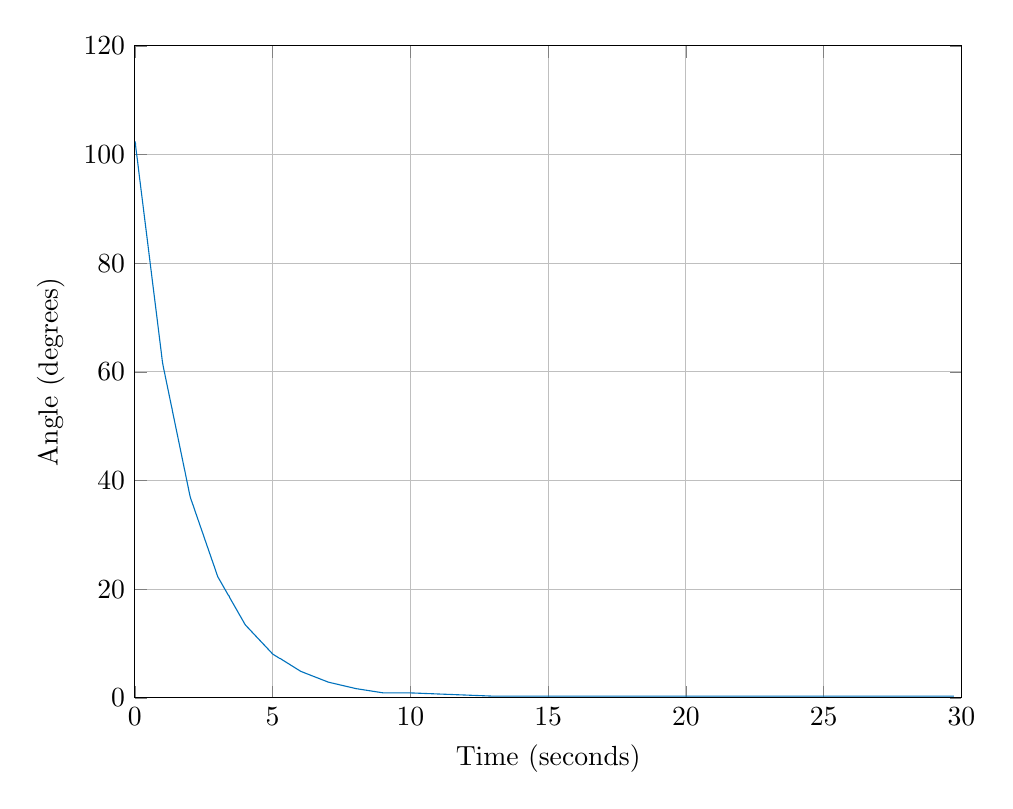
\begin{tikzpicture}

\begin{axis}[%
width=4.133in,
height=3.26in,
at={(0.693in,0.44in)},
scale only axis,
xmin=0,
xmax=30,
xmajorgrids,
xlabel={Time (seconds)},
ymin=0,
ymax=120,
ymajorgrids,
ylabel={Angle (degrees)},
axis background/.style={fill=white}
]
\addplot [color=mycolor1,solid,forget plot]
  table[row sep=crcr]{%
0	102.4204\\
0.0209938430000003	102.0984\\
0.032725631000001	101.3524\\
0.047907375	100.7304\\
0.0639060380000006	100.1084\\
0.0799239030000009	99.4604\\
0.0981854360000007	98.7804\\
0.113220052000001	98.1264\\
0.128292339000002	97.4824\\
0.144036158	96.8304\\
0.160058423	96.1444\\
0.176025763	95.4984\\
0.192056521000002	94.8584\\
0.208000151000001	94.2064\\
0.224035953000002	93.5404\\
0.240121110000001	92.8984\\
0.256026600000001	92.2504\\
0.272110880000001	91.6044\\
0.288031233000001	90.9544\\
0.304005701001001	90.3044\\
0.320010104	89.6504\\
0.336025713000001	88.9944\\
0.352118993000001	88.3444\\
0.368006588000001	87.6964\\
0.384068385001	87.0404\\
0.400018888	86.3864\\
0.416078486000001	85.7344\\
0.431960775	85.0824\\
0.448059412	84.4264\\
0.464393653000001	83.7744\\
0.480023499	83.1184\\
0.496105058	82.4684\\
0.512065969	81.8104\\
0.528102755999001	81.1564\\
0.544123071	80.5024\\
0.560076244000001	79.8204\\
0.576008033	79.1764\\
0.592067592	78.5364\\
0.608003100000001	77.8824\\
0.624140849000001	77.2104\\
0.640006451000001	76.5664\\
0.656002516000001	75.9184\\
0.672034923	75.2764\\
0.688035163000001	74.6224\\
0.704072376	73.9744\\
0.719998864	73.3204\\
0.735996768000001	72.6684\\
0.752079109000001	72.0124\\
0.768246627	71.3624\\
0.784068256999001	70.7024\\
0.800046306	70.0544\\
0.816249501	69.4004\\
0.832013545	68.7404\\
0.848040525	68.0924\\
0.864385085000001	67.4384\\
0.880256688000001	66.7784\\
0.896092370000001	66.1324\\
0.912056074000001	65.4824\\
0.928048759000001	64.8284\\
0.944056606000001	64.1704\\
0.960020854	63.5164\\
0.976001554000001	62.8544\\
0.992006309	62.1624\\
1.008005556	61.6104\\
1.025614861	61.1144\\
1.040589773	60.7284\\
1.055878027	60.3404\\
1.074015929	59.9324\\
1.088938585	59.5604\\
1.104106374	59.1644\\
1.120007369	58.7744\\
1.136007578	58.3904\\
1.152071130999	58.0024\\
1.16806061	57.6124\\
1.184071445	57.2184\\
1.200150768	56.8264\\
1.21615164	56.4324\\
1.232010173	56.0404\\
1.248053376	55.6284\\
1.264288496	55.2444\\
1.280028884	54.8504\\
1.295952573	54.4644\\
1.312037235	54.0744\\
1.328052614	53.6824\\
1.346338536	53.2764\\
1.361453655	52.8504\\
1.376487485001	52.4704\\
1.392056453	52.0904\\
1.408067061	51.7064\\
1.424104207	51.3184\\
1.440033057	50.9264\\
1.456008887	50.5344\\
1.472047327999	50.1284\\
1.488025542	49.7384\\
1.504076592	49.3504\\
1.520002002	48.9604\\
1.536000087	48.5744\\
1.552076278	48.1784\\
1.56802456	47.7804\\
1.58402701	47.3884\\
1.59999875	46.9984\\
1.616051927	46.6204\\
1.631923395	46.2064\\
1.648080439001	45.8124\\
1.663922298	45.4264\\
1.680098942	45.0304\\
1.696047505	44.6364\\
1.712048305	44.2444\\
1.728038296	43.8384\\
1.744090855	43.4504\\
1.760154303	43.0564\\
1.775995371	42.6704\\
1.79192573	42.2644\\
1.810229831	41.8604\\
1.825644686	41.4744\\
1.841053209	41.0864\\
1.856405075	40.6984\\
1.872011649	40.3084\\
1.887965123	39.9244\\
1.904134095	39.5244\\
1.920101638	39.1344\\
1.936330285	38.7364\\
1.952107365001	38.3424\\
1.967909304	37.9504\\
1.984037244	37.5604\\
1.999911404	37.1724\\
2.020476961	36.8104\\
2.032155817	36.6004\\
2.047896624	36.3724\\
2.063919065999	36.1444\\
2.07992118	35.9064\\
2.098217726	35.6644\\
2.113376885	35.4364\\
2.128620225	35.2044\\
2.143993076	34.9744\\
2.159997494	34.7364\\
2.17595988	34.5004\\
2.192083339	34.2704\\
2.208058577999	34.0284\\
2.223942407	33.8004\\
2.239931824	33.5644\\
2.255880643	33.3284\\
2.272087455	33.0984\\
2.288038734	32.8604\\
2.304123209	32.6284\\
2.320046148	32.3844\\
2.336009163	32.1544\\
2.352205507	31.9184\\
2.368133077	31.6884\\
2.384178162	31.4484\\
2.400130171	31.2184\\
2.4163145	30.9784\\
2.432031654	30.7464\\
2.448037416	30.5124\\
2.466558546	30.2704\\
2.4818745	30.0384\\
2.49714429	29.8044\\
2.512372966999	29.5744\\
2.528045724	29.3384\\
2.544099731	29.1104\\
2.56010861	28.8684\\
2.576034922	28.6364\\
2.592095589	28.4024\\
2.608010961	28.1664\\
2.624122969	27.9324\\
2.640033746	27.7004\\
2.656076221	27.4624\\
2.672001898	27.2304\\
2.688022517	26.9964\\
2.703952295	26.7604\\
2.720009942	26.5284\\
2.735925901	26.2904\\
2.753963102	26.0484\\
2.768891909	25.8184\\
2.783841482	25.5844\\
2.799850208	25.3464\\
2.817863062	25.1104\\
2.832955858	24.8724\\
2.847848904	24.6424\\
2.865968994	24.4024\\
2.881728832	24.1724\\
2.896708324	23.9384\\
2.911857664	23.7084\\
2.93004444	23.4644\\
2.943992984	23.2384\\
2.960138534	23.0084\\
2.975914914	22.7704\\
2.99208249	22.5304\\
3.008125313	22.3164\\
3.025357597999	22.1444\\
3.04048063	22.0104\\
3.055927084	21.8684\\
3.071910621	21.7324\\
3.087926493999	21.5904\\
3.103949931	21.4504\\
3.121408746	21.3024\\
3.136617240001	21.1584\\
3.152347755999	21.0164\\
3.168786704	20.8744\\
3.184007514	20.7344\\
3.200145622	20.5984\\
3.216188228	20.4524\\
3.231933557	20.3124\\
3.247919379	20.1624\\
3.26388381	20.0244\\
3.279922539999	19.8844\\
3.296114052	19.7424\\
3.312059619	19.5984\\
3.328066934	19.4544\\
3.344004262	19.3164\\
3.36006398	19.1704\\
3.376005523	19.0284\\
3.392077519	18.8884\\
3.42410739	18.7164\\
3.427029824	18.6004\\
3.439936361	18.4664\\
3.455929345	18.3244\\
3.472523607	18.1824\\
3.487938338	18.0384\\
3.504048917	17.8904\\
3.519996112	17.7524\\
3.535900043	17.6104\\
3.55191439	17.4684\\
3.568120362	17.3264\\
3.583949523	17.1864\\
3.600114973	17.0444\\
3.616031683	16.9004\\
3.632586001	16.7604\\
3.648044518	16.6184\\
3.666364008	16.4684\\
3.681591462	16.3244\\
3.696741885	16.1864\\
3.711996204	16.0464\\
3.728392281001	15.9084\\
3.743904197	15.7604\\
3.759902297	15.6144\\
3.775916481	15.4744\\
3.791846822	15.3344\\
3.808042193	15.1944\\
3.823902876	15.0564\\
3.841964556	14.9084\\
3.855936818	14.7744\\
3.871908187	14.6304\\
3.887887264	14.4884\\
3.903855505	14.3464\\
3.919878531	14.2004\\
3.937950511	14.0584\\
3.951884424	13.9144\\
3.967895965	13.7724\\
3.983853604	13.6324\\
4.001877139	13.4944\\
4.015921822	13.3724\\
4.031854043	13.2904\\
4.049936285	13.2064\\
4.064794501	13.1204\\
4.08015581	13.0324\\
4.095887569001	12.9504\\
4.11186146	12.8624\\
4.127872051999	12.7764\\
4.145974508	12.6884\\
4.160917566	12.6044\\
4.175881287001	12.5204\\
4.191880904	12.4364\\
4.209934432	12.3444\\
4.225387448	12.2564\\
4.240294504001	12.1724\\
4.255905259	12.0884\\
4.271858393999	12.0004\\
4.288019259	11.9144\\
4.303858915	11.8304\\
4.321947523	11.7424\\
4.336842859	11.6564\\
4.351931622	11.5684\\
4.367917727	11.4864\\
4.383910736	11.3984\\
4.399915437	11.3124\\
4.415905531	11.2264\\
4.431887604	11.1384\\
4.450139189	11.0524\\
4.464232905001	10.9624\\
4.479869595001	10.8784\\
4.497933914	10.7904\\
4.512954818	10.7084\\
4.52825885	10.6204\\
4.544208869	10.5364\\
4.560060096	10.4464\\
4.576128848	10.3624\\
4.591916571	10.2764\\
4.60814828	10.1924\\
4.62407138	10.1024\\
4.640194906999	10.0164\\
4.656053299	9.93039999999999\\
4.672041468	9.84439999999998\\
4.688254581	9.75839999999999\\
4.704285816	9.67439999999999\\
4.720037818	9.58839999999999\\
4.736099963	9.50039999999998\\
4.752458547	9.4164\\
4.767997814	9.3304\\
4.784063713	9.2444\\
4.800040788999	9.15639999999999\\
4.815948494	9.07039999999999\\
4.831964013	8.98439999999999\\
4.848003205	8.8964\\
4.86391774	8.81039999999999\\
4.880106925001	8.72439999999999\\
4.896129289	8.63839999999999\\
4.91217689	8.5544\\
4.928060256	8.46639999999999\\
4.944111657	8.38039999999999\\
4.959950621	8.2884\\
4.976098325	8.20439999999999\\
4.992093688	8.1164\\
5.007859106	8.0424\\
5.025322951	7.97839999999999\\
5.040287470001	7.93440000000001\\
5.055939593	7.8844\\
5.07187363	7.83040000000001\\
5.087944269	7.77839999999999\\
5.103960305	7.73039999999999\\
5.120073449	7.68039999999999\\
5.136120004	7.63039999999999\\
5.151881399	7.5784\\
5.170160494	7.5264\\
5.185648884	7.47639999999998\\
5.200895301	7.42639999999999\\
5.216226345	7.37439999999999\\
5.232211896	7.3244\\
5.247879635	7.27439999999999\\
5.281823448	7.21039999999999\\
5.300323869	7.15839999999999\\
5.315590605	7.10839999999999\\
5.330928008	7.05640000000001\\
5.34608405	7.00840000000001\\
5.362068204	6.9564\\
5.378004758	6.90639999999999\\
5.394060244	6.85639999999998\\
5.410031202	6.8064\\
5.426035881	6.7544\\
5.442126566	6.7024\\
5.457991469	6.65239999999999\\
5.473902697	6.60239999999999\\
5.490034384	6.55239999999999\\
5.506000787	6.50239999999999\\
5.52190207	6.45039999999999\\
5.538151371	6.3984\\
5.553984983	6.34639999999999\\
5.570298147	6.29839999999999\\
5.585942519	6.2484\\
5.603382692	6.1964\\
5.618664619	6.14439999999999\\
5.634047836	6.09439999999999\\
5.649998673	6.0444\\
5.666094419	5.9924\\
5.681841182	5.94239999999999\\
5.699907156	5.8904\\
5.714762218	5.84239999999998\\
5.729844038	5.79040000000001\\
5.74784322	5.73840000000001\\
5.762729151	5.6904\\
5.777860622	5.6384\\
5.795907101	5.5864\\
5.810774976	5.53439999999998\\
5.825865781001	5.48639999999999\\
5.843919216	5.43440000000001\\
5.859290632	5.3824\\
5.874185852	5.33439999999999\\
5.890072566	5.28239999999998\\
5.906023474	5.23239999999998\\
5.921823309	5.1824\\
5.939928715	5.13039999999999\\
5.954799261	5.08239999999999\\
5.969820941	5.03039999999999\\
5.987853738	4.97839999999999\\
6.002981258	4.92640000000002\\
6.017828536	4.88039999999999\\
6.033823127	4.8404\\
6.049868696	4.8104\\
6.067922867	4.7764\\
6.082838751	4.7444\\
6.097900682	4.7144\\
6.113849356	4.68440000000001\\
6.129827063	4.6524\\
6.148023071	4.62039999999999\\
6.163092169001	4.5864\\
6.177986784	4.55639999999998\\
6.193915542	4.52239999999999\\
6.211929221	4.48839999999998\\
6.226789927	4.4584\\
6.241816336	4.42839999999998\\
6.259884345	4.39439999999999\\
6.274859058	4.36439999999997\\
6.289822502	4.3344\\
6.307910192	4.30239999999999\\
6.323024645	4.27239999999999\\
6.337912525	4.23839999999998\\
6.354315097	4.2064\\
6.369813751	4.17639999999999\\
6.387941284	4.14239999999999\\
6.403272567	4.11239999999998\\
6.418280023	4.08239999999999\\
6.433834917	4.04839999999999\\
6.449903337	4.0164\\
6.465818905	3.98639999999997\\
6.481852265	3.9524\\
6.4978292	3.9204\\
6.513928642	3.8904\\
6.529850342999	3.85839999999999\\
6.545926012	3.82640000000001\\
6.561928695	3.79639999999999\\
6.577838841	3.7624\\
6.595872073	3.73039999999999\\
6.611486670999	3.69839999999999\\
6.627109471	3.66639999999998\\
6.642128122	3.6384\\
6.657865058	3.60639999999998\\
6.673839925	3.5744\\
6.691861475	3.5424\\
6.706804182001	3.5124\\
6.722093433	3.47639999999998\\
6.737826331	3.4464\\
6.753858422	3.41239999999999\\
6.769850097999	3.38039999999999\\
6.78586044	3.3484\\
6.801863013	3.32040000000001\\
6.817822903	3.28639999999999\\
6.835912873	3.2544\\
6.850797684	3.22239999999999\\
6.865816812	3.19239999999999\\
6.883888539	3.16239999999999\\
6.899406692	3.13040000000001\\
6.914267148	3.09439999999999\\
6.92979835	3.06440000000001\\
6.947817364	3.0324\\
6.9626418	3.00239999999999\\
6.977816625	2.9684\\
6.993859934	2.9384\\
7.009821383	2.90639999999999\\
7.027336129	2.88040000000001\\
7.042246952999	2.8604\\
7.057822284	2.8424\\
7.07586737	2.82239999999999\\
7.090775321	2.80239999999999\\
7.105829495	2.7824\\
7.123931186	2.7624\\
7.138774464	2.7424\\
7.153833061	2.72239999999999\\
7.171913071	2.7064\\
7.187338123	2.6884\\
7.202934031999	2.67239999999998\\
7.218397429	2.6524\\
7.233820685	2.6324\\
7.251968867999	2.61239999999999\\
7.265885502	2.5924\\
7.281865289	2.57239999999999\\
7.299884868999	2.55239999999999\\
7.31476638	2.53439999999999\\
7.329867748	2.5184\\
7.347930791	2.49839999999999\\
7.362852106	2.48239999999998\\
7.377837717	2.46040000000001\\
7.395892001	2.44239999999999\\
7.410776928	2.42239999999998\\
7.425819193	2.4024\\
7.443864556	2.3824\\
7.458788003	2.36239999999999\\
7.473887773	2.3424\\
7.489857742	2.3284\\
7.50583103	2.30840000000001\\
7.521851319	2.29039999999999\\
7.537810362	2.27239999999999\\
7.555906413	2.25239999999999\\
7.571284413	2.23239999999998\\
7.586918532	2.2124\\
7.601858076	2.19239999999999\\
7.619953905	2.17239999999998\\
7.634872726	2.1524\\
7.649859506	2.13640000000001\\
7.667959938	2.1164\\
7.68290233	2.10039999999999\\
7.69791371	2.08240000000001\\
7.713855764	2.0624\\
7.729968987	2.04239999999999\\
7.745903562	2.02239999999999\\
7.764114133	2.00239999999999\\
7.77936898	1.98239999999998\\
7.794252915	1.9624\\
7.809892049	1.9464\\
7.825842332001	1.92639999999999\\
7.843860135	1.9084\\
7.858703643	1.89239999999999\\
7.873820098	1.8724\\
7.891893728	1.85239999999999\\
7.906862227	1.83240000000001\\
7.921959541	1.8124\\
7.940014419	1.79239999999999\\
7.954986679	1.77239999999999\\
7.969991037	1.7544\\
7.985956232	1.7384\\
8.001834331	1.7204\\
8.019008353	1.7024\\
8.033860325	1.6844\\
8.051885708	1.67039999999999\\
8.066781052	1.6584\\
8.08185164	1.6464\\
8.097826547	1.6344\\
8.115886825	1.62039999999999\\
8.130993767001	1.60839999999999\\
8.146272727	1.59639999999999\\
8.161866375	1.5844\\
8.180021206	1.57039999999999\\
8.195029494	1.55639999999998\\
8.210085624	1.54639999999999\\
8.225968383	1.53439999999999\\
8.241977698	1.5204\\
8.257958223	1.50639999999999\\
8.273980683	1.4944\\
8.289979354	1.48239999999998\\
8.306105022	1.4684\\
8.321961807	1.4564\\
8.337956599	1.4444\\
8.354008421	1.43039999999999\\
8.369916341	1.41839999999999\\
8.385982796	1.4044\\
8.401996711	1.39439999999999\\
8.417953928	1.38040000000001\\
8.433969553	1.36639999999998\\
8.44994668	1.3544\\
8.465916425	1.34439999999999\\
8.482074673	1.3304\\
8.498137695	1.3164\\
8.513989218	1.30439999999999\\
8.530018823	1.29239999999999\\
8.546166983	1.2784\\
8.56215515	1.2664\\
8.578147953	1.25239999999999\\
8.594112176	1.24039999999999\\
8.610104207	1.22639999999998\\
8.625964940999	1.21639999999999\\
8.641894706	1.20439999999999\\
8.657993463	1.1904\\
8.673949317	1.17639999999999\\
8.689937499	1.16439999999999\\
8.705959609001	1.1544\\
8.722137315	1.1404\\
8.738011636	1.12639999999999\\
8.754108077	1.11439999999999\\
8.769995601	1.10039999999999\\
8.786068468	1.08840000000001\\
8.802090489	1.07639999999999\\
8.818056321	1.06440000000001\\
8.834055568	1.0504\\
8.849943263	1.0384\\
8.865977143001	1.0264\\
8.881911558999	1.01439999999999\\
8.897921601	1.00039999999998\\
8.913976559	0.986399999999989\\
8.929943874	0.974399999999989\\
8.945953124	0.964399999999998\\
8.961948839	0.948399999999992\\
8.977871706	0.936399999999992\\
8.993870588	0.924399999999991\\
9.00984736	0.910399999999996\\
9.026860699	0.9024\\
9.041861293	0.900400000000005\\
9.060100216	0.900400000000005\\
9.075336024	0.900400000000005\\
9.09082378	0.900400000000005\\
9.106020972999	0.900400000000005\\
9.122236741	0.900400000000005\\
9.138166787	0.900400000000005\\
9.154034185	0.900400000000005\\
9.170133264	0.900400000000005\\
9.186129414	0.900400000000005\\
9.20211939	0.900400000000005\\
9.218032884	0.900400000000005\\
9.233966006	0.900400000000005\\
9.249970896	0.900400000000005\\
9.265816294	0.900400000000005\\
9.281798301999	0.900400000000005\\
9.297988874	0.900400000000005\\
9.313975212	0.900400000000005\\
9.329991468	0.900400000000005\\
9.346091804	0.900400000000005\\
9.361975074	0.900400000000005\\
9.377773317	0.900400000000005\\
9.393796624	0.900400000000005\\
9.409791762	0.900400000000005\\
9.425783104	0.900400000000005\\
9.441863749	0.900400000000005\\
9.458013219	0.900400000000005\\
9.473933061	0.900400000000005\\
9.490172847	0.900400000000005\\
9.506105225	0.900400000000005\\
9.522117011	0.900400000000005\\
9.537993179	0.900400000000005\\
9.553971228	0.900400000000005\\
9.569939019	0.900400000000005\\
9.588105311	0.900400000000005\\
9.603152707	0.900400000000005\\
9.618217492	0.900400000000005\\
9.634147989	0.900400000000005\\
9.649948571	0.900400000000005\\
9.665877124999	0.900400000000005\\
9.682002717	0.900400000000005\\
9.698247531	0.900400000000005\\
9.714098186	0.900400000000005\\
9.729973102001	0.900400000000005\\
9.745908845	0.900400000000005\\
9.762252578	0.900400000000005\\
9.77812166	0.900400000000005\\
9.793984073	0.900400000000005\\
9.809942462	0.900400000000005\\
9.826049278	0.900400000000005\\
9.842098384	0.900400000000005\\
9.85805312	0.900400000000005\\
9.874101799	0.900400000000005\\
9.890141022	0.900400000000005\\
9.906026853001	0.900400000000005\\
9.921913004	0.900400000000005\\
9.937905661	0.900400000000005\\
9.953974857	0.900400000000005\\
9.970019312	0.900400000000005\\
9.985981670999	0.900400000000005\\
10.001982251	0.900400000000005\\
10.019429092	0.900400000000005\\
10.034424784	0.900400000000005\\
10.049875015	0.892399999999995\\
10.065850456	0.8904\\
10.08182818	0.8904\\
10.097959543	0.888400000000004\\
10.113958375	0.880400000000009\\
10.129909538	0.880400000000009\\
10.145944196	0.878399999999985\\
10.16196201	0.870399999999989\\
10.177909556	0.870399999999989\\
10.193945621	0.868399999999994\\
10.209958279	0.860399999999998\\
10.226076476	0.860399999999998\\
10.24228651	0.860399999999998\\
10.258125425	0.850399999999993\\
10.274162457	0.850399999999993\\
10.290295893999	0.850399999999993\\
10.306107224	0.842399999999998\\
10.322085987	0.840400000000002\\
10.33809667	0.840400000000002\\
10.354106872	0.832400000000007\\
10.370134729	0.830400000000012\\
10.385951122	0.830400000000012\\
10.401988865	0.824399999999997\\
10.417967958	0.820399999999992\\
10.434112444	0.820399999999992\\
10.450095951	0.818399999999997\\
10.46626591	0.810399999999987\\
10.482040985	0.810399999999987\\
10.498092205	0.808399999999992\\
10.514405684	0.800399999999996\\
10.530130393999	0.800399999999996\\
10.546145618	0.800399999999996\\
10.561964276	0.790400000000005\\
10.577948549	0.790400000000005\\
10.593931009	0.790400000000005\\
10.6101085	0.7804\\
10.626091174	0.7804\\
10.641975592	0.7804\\
10.657987333	0.772400000000005\\
10.673937919001	0.770399999999995\\
10.690006367999	0.770399999999995\\
10.706012607	0.764399999999995\\
10.721981149	0.760400000000004\\
10.738063726	0.760400000000004\\
10.754020226	0.756399999999985\\
10.769985922	0.750399999999985\\
10.785997287	0.750399999999985\\
10.801974595	0.74839999999999\\
10.81798408	0.740399999999994\\
10.833961914	0.740399999999994\\
10.850012348	0.738399999999999\\
10.86605352	0.730399999999989\\
10.881839524	0.730399999999989\\
10.897935746	0.730399999999989\\
10.913958502	0.720399999999998\\
10.930041754	0.720399999999998\\
10.945980494	0.720399999999998\\
10.961984783	0.712400000000002\\
10.978042258	0.710400000000007\\
10.99404158	0.710400000000007\\
11.010176995	0.702400000000011\\
11.025855525	0.700400000000016\\
11.041804922	0.700400000000016\\
11.059913384	0.694400000000002\\
11.074824358	0.690399999999983\\
11.089869129	0.690399999999983\\
11.107951026	0.686399999999992\\
11.122984172	0.680399999999992\\
11.138342242	0.680399999999992\\
11.154040147	0.678399999999996\\
11.169921647	0.670400000000001\\
11.185965706	0.670400000000001\\
11.201934188	0.670400000000001\\
11.217937182001	0.660399999999996\\
11.234010419	0.660399999999996\\
11.250017576	0.660399999999996\\
11.265963013	0.650400000000005\\
11.281984233	0.650400000000005\\
11.298001456	0.650400000000005\\
11.314013084	0.642399999999995\\
11.32995111	0.6404\\
11.345984562	0.6404\\
11.362110719	0.634399999999999\\
11.378218492	0.630400000000009\\
11.394123842	0.630400000000009\\
11.410127549	0.62639999999999\\
11.426115205	0.620399999999989\\
11.442158633	0.620399999999989\\
11.457998163	0.618399999999994\\
11.474088567	0.610399999999998\\
11.490214531	0.610399999999998\\
11.506218814999	0.608399999999989\\
11.522124566	0.600399999999993\\
11.538143643	0.600399999999993\\
11.553959735	0.598399999999998\\
11.570094389	0.590400000000002\\
11.586108681	0.590400000000002\\
11.601997267	0.590400000000002\\
11.617937676	0.580400000000012\\
11.634047545	0.580400000000012\\
11.649961358	0.580400000000012\\
11.665939953999	0.572399999999988\\
11.681983171	0.570399999999992\\
11.697944301	0.568399999999997\\
11.71410734	0.562399999999997\\
11.729976237	0.560399999999987\\
11.746017163999	0.558399999999992\\
11.761969003	0.556399999999996\\
11.778114573	0.550399999999996\\
11.79414493	0.550399999999996\\
11.810082187	0.546399999999991\\
11.826148542	0.540400000000005\\
11.842074879	0.540400000000005\\
11.857881383	0.538399999999996\\
11.873828401	0.5304\\
11.889954814	0.5304\\
11.906002506	0.528399999999991\\
11.921994858	0.520399999999995\\
11.937993593	0.520399999999995\\
11.954119782999	0.5184\\
11.97010989	0.510400000000004\\
11.986060563	0.510400000000004\\
12.002017814001	0.508400000000009\\
12.019620008	0.502399999999994\\
12.034616554	0.500399999999985\\
12.050022968	0.49839999999999\\
12.065906013	0.494399999999999\\
12.081957784	0.490399999999994\\
12.097933417	0.490399999999994\\
12.113798944	0.486400000000003\\
12.129973495	0.480399999999989\\
12.14610355	0.480399999999989\\
12.161956852	0.476399999999984\\
12.177949554	0.470399999999998\\
12.193952771	0.470399999999998\\
12.20995285	0.468400000000003\\
12.22592261	0.460400000000007\\
12.241962385	0.460400000000007\\
12.258050298	0.458400000000012\\
12.274086128	0.450400000000016\\
12.289913336	0.450400000000016\\
12.306040873	0.448399999999992\\
12.322231529	0.440399999999983\\
12.338093841	0.440399999999983\\
12.354023591	0.438399999999987\\
12.370083285	0.432400000000001\\
12.386078558999	0.430399999999992\\
12.402190226	0.430399999999992\\
12.418103744	0.426400000000001\\
12.43407151	0.420400000000001\\
12.450099973	0.420400000000001\\
12.466132516	0.416399999999982\\
12.482114334	0.410399999999996\\
12.498153141	0.410399999999996\\
12.51409142	0.4084\\
12.529965314	0.400400000000005\\
12.54596624	0.400400000000005\\
12.561950563	0.398399999999995\\
12.578147653	0.3904\\
12.594269473	0.3904\\
12.610438881	0.388400000000004\\
12.626097016	0.380400000000009\\
12.642095892	0.380400000000009\\
12.658089341	0.378400000000013\\
12.673962283	0.372399999999999\\
12.68990182	0.370399999999989\\
12.706080489	0.368399999999994\\
12.72219824	0.364400000000003\\
12.738346594	0.360399999999998\\
12.753967274	0.360399999999998\\
12.769940242	0.356399999999979\\
12.785950274001	0.350399999999993\\
12.801946294	0.350399999999993\\
12.817940319	0.346399999999988\\
12.833938895	0.340400000000002\\
12.849974966	0.340400000000002\\
12.865960181	0.338400000000007\\
12.881945562	0.330400000000012\\
12.897950342	0.330400000000012\\
12.913976611	0.328400000000016\\
12.929964422	0.320399999999992\\
12.945935771	0.320399999999992\\
12.962009429	0.318399999999997\\
12.977968218	0.310399999999987\\
12.993942423	0.310399999999987\\
13.012185494	0.310399999999987\\
13.026070987999	0.310399999999987\\
13.041848179	0.308399999999992\\
13.059885922	0.308399999999992\\
13.07473698	0.308399999999992\\
13.089830741	0.308399999999992\\
13.105901108	0.308399999999992\\
13.124259858	0.308399999999992\\
13.139574647	0.308399999999992\\
13.154908367	0.308399999999992\\
13.170070864	0.308399999999992\\
13.185980002	0.308399999999992\\
13.201938231	0.308399999999992\\
13.21805493	0.308399999999992\\
13.23402567	0.308399999999992\\
13.249914325	0.308399999999992\\
13.266175359	0.308399999999992\\
13.282239574	0.308399999999992\\
13.297971832	0.308399999999992\\
13.313949505	0.308399999999992\\
13.33009573	0.308399999999992\\
13.346079127	0.308399999999992\\
13.362036705	0.308399999999992\\
13.378117366	0.308399999999992\\
13.394194991	0.308399999999992\\
13.410321121	0.308399999999992\\
13.425924015	0.308399999999992\\
13.442134772	0.308399999999992\\
13.457936676999	0.308399999999992\\
13.473935864	0.308399999999992\\
13.489955753	0.308399999999992\\
13.505945675	0.308399999999992\\
13.52191076	0.308399999999992\\
13.540084122	0.308399999999992\\
13.555082006	0.308399999999992\\
13.570144396	0.308399999999992\\
13.585963339	0.308399999999992\\
13.602119768001	0.308399999999992\\
13.617959113	0.308399999999992\\
13.634099019	0.308399999999992\\
13.65004466	0.308399999999992\\
13.665959361	0.308399999999992\\
13.682036179	0.308399999999992\\
13.697948277	0.308399999999992\\
13.713888352	0.308399999999992\\
13.729975701	0.308399999999992\\
13.745822185	0.308399999999992\\
13.764013712	0.308399999999992\\
13.779074681	0.308399999999992\\
13.79411913	0.308399999999992\\
13.810453842	0.308399999999992\\
13.826119213	0.308399999999992\\
13.842102805	0.308399999999992\\
13.858004651	0.308399999999992\\
13.874148209999	0.308399999999992\\
13.890211438	0.308399999999992\\
13.906026639	0.308399999999992\\
13.921929532999	0.308399999999992\\
13.937930293	0.308399999999992\\
13.953949666	0.308399999999992\\
13.970014126	0.308399999999992\\
13.985952415	0.308399999999992\\
14.001954349	0.308399999999992\\
14.019356205	0.308399999999992\\
14.0345781	0.308399999999992\\
14.050046454	0.308399999999992\\
14.065963735999	0.308399999999992\\
14.081962959	0.308399999999992\\
14.097958688001	0.308399999999992\\
14.113962925	0.308399999999992\\
14.129868291	0.308399999999992\\
14.145976169001	0.308399999999992\\
14.162018735	0.308399999999992\\
14.177967824	0.308399999999992\\
14.193951521	0.308399999999992\\
14.209955202999	0.308399999999992\\
14.225945746	0.308399999999992\\
14.242095374	0.308399999999992\\
14.258084378	0.308399999999992\\
14.273966584999	0.308399999999992\\
14.290070074	0.308399999999992\\
14.306151306	0.308399999999992\\
14.322157069	0.308399999999992\\
14.338127065	0.308399999999992\\
14.354027804	0.308399999999992\\
14.370091707	0.308399999999992\\
14.386173707	0.308399999999992\\
14.402152308	0.308399999999992\\
14.417962778	0.308399999999992\\
14.433898872	0.308399999999992\\
14.449937669	0.308399999999992\\
14.46594541	0.308399999999992\\
14.481936153	0.308399999999992\\
14.497949072	0.308399999999992\\
14.514088191	0.308399999999992\\
14.530025959	0.308399999999992\\
14.545945851	0.308399999999992\\
14.561976985999	0.308399999999992\\
14.577952635	0.308399999999992\\
14.593999129	0.308399999999992\\
14.609836154	0.308399999999992\\
14.625803495	0.308399999999992\\
14.641834721	0.308399999999992\\
14.657813307	0.308399999999992\\
14.674097502	0.308399999999992\\
14.690199387	0.308399999999992\\
14.70596728	0.308399999999992\\
14.721979587	0.308399999999992\\
14.737937862	0.308399999999992\\
14.754111298	0.308399999999992\\
14.770142483	0.308399999999992\\
14.786091036	0.308399999999992\\
14.80213982	0.308399999999992\\
14.818128333	0.308399999999992\\
14.834127511	0.308399999999992\\
14.850141901999	0.308399999999992\\
14.865869091	0.308399999999992\\
14.882147262	0.308399999999992\\
14.89804579	0.308399999999992\\
14.914096931	0.308399999999992\\
14.930118164	0.308399999999992\\
14.945939577999	0.308399999999992\\
14.961906391	0.308399999999992\\
14.978083557	0.308399999999992\\
14.994194693	0.308399999999992\\
15.010243883	0.308399999999992\\
15.027569009	0.308399999999992\\
15.042725340001	0.308399999999992\\
15.058146249	0.308399999999992\\
15.073950314001	0.308399999999992\\
15.08993781	0.308399999999992\\
15.106009993	0.308399999999992\\
15.121964524	0.308399999999992\\
15.1380098	0.308399999999992\\
15.154009925	0.308399999999992\\
15.169993757	0.308399999999992\\
15.186005332	0.308399999999992\\
15.201995098	0.308399999999992\\
15.217951559	0.308399999999992\\
15.233949117	0.308399999999992\\
15.249978112	0.308399999999992\\
15.26594244	0.308399999999992\\
15.281927479999	0.308399999999992\\
15.297954920999	0.308399999999992\\
15.316441037	0.308399999999992\\
15.331490864	0.308399999999992\\
15.346654893999	0.308399999999992\\
15.362019403	0.308399999999992\\
15.378044634	0.308399999999992\\
15.394024999	0.308399999999992\\
15.410121712	0.308399999999992\\
15.426140864	0.308399999999992\\
15.442144156	0.308399999999992\\
15.458102726	0.308399999999992\\
15.474067155	0.308399999999992\\
15.490170949	0.308399999999992\\
15.50611001	0.308399999999992\\
15.522123419001	0.308399999999992\\
15.538128811	0.308399999999992\\
15.554167397	0.308399999999992\\
15.570317406	0.308399999999992\\
15.586086056	0.308399999999992\\
15.602042431	0.308399999999992\\
15.617914345	0.308399999999992\\
15.633947314	0.308399999999992\\
15.649946357	0.308399999999992\\
15.665936502	0.308399999999992\\
15.681995740001	0.308399999999992\\
15.697981437	0.308399999999992\\
15.714114623	0.308399999999992\\
15.729968049	0.308399999999992\\
15.745973241	0.308399999999992\\
15.761975013	0.308399999999992\\
15.777977313	0.308399999999992\\
15.793950055	0.308399999999992\\
15.810053864	0.308399999999992\\
15.826109715	0.308399999999992\\
15.8420769	0.308399999999992\\
15.857990297	0.308399999999992\\
15.873952576	0.308399999999992\\
15.889927934	0.308399999999992\\
15.905928504001	0.308399999999992\\
15.921917352	0.308399999999992\\
15.937880098	0.308399999999992\\
15.953946858	0.308399999999992\\
15.970227598	0.308399999999992\\
15.98611852	0.308399999999992\\
16.002091267	0.308399999999992\\
16.020011446	0.308399999999992\\
16.035348698	0.308399999999992\\
16.050859244	0.308399999999992\\
16.066272319	0.308399999999992\\
16.081955224	0.308399999999992\\
16.09810599	0.308399999999992\\
16.114094623	0.308399999999992\\
16.130088814	0.308399999999992\\
16.146124849	0.308399999999992\\
16.16213664	0.308399999999992\\
16.177952983	0.308399999999992\\
16.194215687	0.308399999999992\\
16.209942352001	0.308399999999992\\
16.226103105	0.308399999999992\\
16.242153955	0.308399999999992\\
16.258129173	0.308399999999992\\
16.274231659	0.308399999999992\\
16.290130769	0.308399999999992\\
16.306107425	0.308399999999992\\
16.322094334	0.308399999999992\\
16.337964334	0.308399999999992\\
16.354028884	0.308399999999992\\
16.369851925	0.308399999999992\\
16.385939184	0.308399999999992\\
16.40216491	0.308399999999992\\
16.418141656	0.308399999999992\\
16.434087918	0.308399999999992\\
16.450115805	0.308399999999992\\
16.466220697	0.308399999999992\\
16.48194438	0.308399999999992\\
16.497942956	0.308399999999992\\
16.514092388	0.308399999999992\\
16.530027611	0.308399999999992\\
16.545940387	0.308399999999992\\
16.561917439	0.308399999999992\\
16.577962596	0.308399999999992\\
16.594091923	0.308399999999992\\
16.610127187	0.308399999999992\\
16.625940217	0.308399999999992\\
16.641920587	0.308399999999992\\
16.657934723	0.308399999999992\\
16.674121098999	0.308399999999992\\
16.690080671	0.308399999999992\\
16.706221689999	0.308399999999992\\
16.722144374	0.308399999999992\\
16.738270022	0.308399999999992\\
16.753968498001	0.308399999999992\\
16.769945004	0.308399999999992\\
16.786098366001	0.308399999999992\\
16.802143672	0.308399999999992\\
16.817969121	0.308399999999992\\
16.833944354	0.308399999999992\\
16.849956285	0.308399999999992\\
16.866084439	0.308399999999992\\
16.882118961	0.308399999999992\\
16.898062046	0.308399999999992\\
16.913936732	0.308399999999992\\
16.92996755	0.308399999999992\\
16.946119569	0.308399999999992\\
16.962189135	0.308399999999992\\
16.977990915	0.308399999999992\\
16.993944183	0.308399999999992\\
17.010028153	0.308399999999992\\
17.027481298	0.308399999999992\\
17.042556051	0.308399999999992\\
17.058157483	0.308399999999992\\
17.07411903	0.308399999999992\\
17.089888024	0.308399999999992\\
17.106001667	0.308399999999992\\
17.121993021	0.308399999999992\\
17.138120965	0.308399999999992\\
17.15400629	0.308399999999992\\
17.169959362	0.308399999999992\\
17.186074773	0.308399999999992\\
17.201965239	0.308399999999992\\
17.218087845	0.308399999999992\\
17.234180144	0.308399999999992\\
17.250190466	0.308399999999992\\
17.266117259	0.308399999999992\\
17.282113449	0.308399999999992\\
17.297879363	0.308399999999992\\
17.31609882	0.308399999999992\\
17.331421431001	0.308399999999992\\
17.347189558	0.308399999999992\\
17.363033569	0.308399999999992\\
17.378512623	0.308399999999992\\
17.394131859	0.308399999999992\\
17.410117265	0.308399999999992\\
17.426122937	0.308399999999992\\
17.442109416	0.308399999999992\\
17.45814933	0.308399999999992\\
17.474101791	0.308399999999992\\
17.489959012	0.308399999999992\\
17.506113986999	0.308399999999992\\
17.522060234	0.308399999999992\\
17.538168779	0.308399999999992\\
17.55409893	0.308399999999992\\
17.570113131	0.308399999999992\\
17.586133919	0.308399999999992\\
17.602030148001	0.308399999999992\\
17.618329869	0.308399999999992\\
17.634104717999	0.308399999999992\\
17.650238806	0.308399999999992\\
17.666262587	0.308399999999992\\
17.68210917	0.308399999999992\\
17.698103687	0.308399999999992\\
17.714134716	0.308399999999992\\
17.729976051	0.308399999999992\\
17.746014762	0.308399999999992\\
17.761955943	0.308399999999992\\
17.778013618	0.308399999999992\\
17.793960588	0.308399999999992\\
17.809899777	0.308399999999992\\
17.825977037	0.308399999999992\\
17.841999447	0.308399999999992\\
17.858016199	0.308399999999992\\
17.873896615	0.308399999999992\\
17.889894225	0.308399999999992\\
17.905943762	0.308399999999992\\
17.922004574	0.308399999999992\\
17.937982854	0.308399999999992\\
17.953991632	0.308399999999992\\
17.97005083	0.308399999999992\\
17.98598706	0.308399999999992\\
18.002001216	0.308399999999992\\
18.019307107	0.308399999999992\\
18.034242008	0.308399999999992\\
18.049918586	0.308399999999992\\
18.065965527	0.308399999999992\\
18.081968739	0.308399999999992\\
18.098119333	0.308399999999992\\
18.114282141	0.308399999999992\\
18.130018637999	0.308399999999992\\
18.146035074	0.308399999999992\\
18.162045652	0.308399999999992\\
18.178001176	0.308399999999992\\
18.193983544	0.308399999999992\\
18.209895278	0.308399999999992\\
18.225974773	0.308399999999992\\
18.242005135	0.308399999999992\\
18.257988347	0.308399999999992\\
18.274008115	0.308399999999992\\
18.290009914	0.308399999999992\\
18.306070014	0.308399999999992\\
18.321933108	0.308399999999992\\
18.337847066	0.308399999999992\\
18.353943443	0.308399999999992\\
18.370041089	0.308399999999992\\
18.386093637	0.308399999999992\\
18.402005877	0.308399999999992\\
18.418044649	0.308399999999992\\
18.434123526999	0.308399999999992\\
18.450072750999	0.308399999999992\\
18.466031802	0.308399999999992\\
18.48198494	0.308399999999992\\
18.498006087	0.308399999999992\\
18.513978649	0.308399999999992\\
18.530007062	0.308399999999992\\
18.546004459999	0.308399999999992\\
18.562116664	0.308399999999992\\
18.577961887	0.308399999999992\\
18.594117103	0.308399999999992\\
18.61016513	0.308399999999992\\
18.62614782	0.308399999999992\\
18.642138323	0.308399999999992\\
18.658129492	0.308399999999992\\
18.673930826001	0.308399999999992\\
18.690115488	0.308399999999992\\
18.706125625	0.308399999999992\\
18.722149674001	0.308399999999992\\
18.738158743	0.308399999999992\\
18.754032035	0.308399999999992\\
18.770227462	0.308399999999992\\
18.785968028	0.308399999999992\\
18.802073351	0.308399999999992\\
18.818019653	0.308399999999992\\
18.834036181	0.308399999999992\\
18.849920083	0.308399999999992\\
18.865905144	0.308399999999992\\
18.881863904	0.308399999999992\\
18.898118502	0.308399999999992\\
18.913973318	0.308399999999992\\
18.930011789	0.308399999999992\\
18.945996468	0.308399999999992\\
18.961957675	0.308399999999992\\
18.978038546	0.308399999999992\\
18.993950119	0.308399999999992\\
19.009979511	0.308399999999992\\
19.026101337	0.308399999999992\\
19.042198975	0.308399999999992\\
19.058058908	0.308399999999992\\
19.073912492	0.308399999999992\\
19.090009825	0.308399999999992\\
19.106012499	0.308399999999992\\
19.122113643	0.308399999999992\\
19.138008253	0.308399999999992\\
19.154018751	0.308399999999992\\
19.170078345	0.308399999999992\\
19.185946931	0.308399999999992\\
19.201958471	0.308399999999992\\
19.217940981	0.308399999999992\\
19.23394118	0.308399999999992\\
19.249947604	0.308399999999992\\
19.265924596	0.308399999999992\\
19.281956066	0.308399999999992\\
19.297999472999	0.308399999999992\\
19.314010142	0.308399999999992\\
19.330010396	0.308399999999992\\
19.346041902	0.308399999999992\\
19.36202181	0.308399999999992\\
19.377967411	0.308399999999992\\
19.39399404	0.308399999999992\\
19.409969835	0.308399999999992\\
19.426283269	0.308399999999992\\
19.442033868	0.308399999999992\\
19.458007326	0.308399999999992\\
19.473993519	0.308399999999992\\
19.490018174	0.308399999999992\\
19.506002918	0.308399999999992\\
19.522009503	0.308399999999992\\
19.537994958	0.308399999999992\\
19.553985961	0.308399999999992\\
19.569972786	0.308399999999992\\
19.585953903	0.308399999999992\\
19.601969868	0.308399999999992\\
19.617984044	0.308399999999992\\
19.633906351	0.308399999999992\\
19.650001898	0.308399999999992\\
19.665971628	0.308399999999992\\
19.681963453	0.308399999999992\\
19.697940772	0.308399999999992\\
19.713999713	0.308399999999992\\
19.729899678	0.308399999999992\\
19.745988171	0.308399999999992\\
19.761997541	0.308399999999992\\
19.777979514	0.308399999999992\\
19.794105228001	0.308399999999992\\
19.810024519	0.308399999999992\\
19.82601676	0.308399999999992\\
19.841989398	0.308399999999992\\
19.857983448	0.308399999999992\\
19.874032654	0.308399999999992\\
19.890013214	0.308399999999992\\
19.906032606	0.308399999999992\\
19.92206543	0.308399999999992\\
19.93794876	0.308399999999992\\
19.95396719	0.308399999999992\\
19.969928617	0.308399999999992\\
19.985960864	0.308399999999992\\
20.001918838	0.308399999999992\\
20.019858791	0.308399999999992\\
20.035345382	0.308399999999992\\
20.050613659	0.308399999999992\\
20.066008056	0.308399999999992\\
20.081908941	0.308399999999992\\
20.097978963	0.308399999999992\\
20.113913681	0.308399999999992\\
20.132141024	0.308399999999992\\
20.147628472001	0.308399999999992\\
20.162961761	0.308399999999992\\
20.178664952	0.308399999999992\\
20.194020201	0.308399999999992\\
20.210065925	0.308399999999992\\
20.226220858	0.308399999999992\\
20.242034084	0.308399999999992\\
20.257999828	0.308399999999992\\
20.274180489	0.308399999999992\\
20.289985065	0.308399999999992\\
20.305972681	0.308399999999992\\
20.322268621	0.308399999999992\\
20.338081768999	0.308399999999992\\
20.353994072	0.308399999999992\\
20.370198002	0.308399999999992\\
20.386044203	0.308399999999992\\
20.401977613	0.308399999999992\\
20.417988835999	0.308399999999992\\
20.434035643001	0.308399999999992\\
20.450040246	0.308399999999992\\
20.466065767	0.308399999999992\\
20.482040359	0.308399999999992\\
20.497936327	0.308399999999992\\
20.513950849	0.308399999999992\\
20.530011164999	0.308399999999992\\
20.545973383	0.308399999999992\\
20.56196601	0.308399999999992\\
20.577949623	0.308399999999992\\
20.593953205	0.308399999999992\\
20.610023563	0.308399999999992\\
20.6259522	0.308399999999992\\
20.641891732	0.308399999999992\\
20.658080268999	0.308399999999992\\
20.674251796	0.308399999999992\\
20.690118794001	0.308399999999992\\
20.705973203	0.308399999999992\\
20.721975833001	0.308399999999992\\
20.738107655	0.308399999999992\\
20.754216286	0.308399999999992\\
20.770098803	0.308399999999992\\
20.786103418	0.308399999999992\\
20.802386499	0.308399999999992\\
20.818133895	0.308399999999992\\
20.834155849	0.308399999999992\\
20.849969862	0.308399999999992\\
20.865900787	0.308399999999992\\
20.881949619	0.308399999999992\\
20.898123567	0.308399999999992\\
20.914119436	0.308399999999992\\
20.929951656	0.308399999999992\\
20.945934124999	0.308399999999992\\
20.961946166	0.308399999999992\\
20.977972179	0.308399999999992\\
20.994080046999	0.308399999999992\\
21.01007956	0.308399999999992\\
21.027794443	0.308399999999992\\
21.04403577	0.308399999999992\\
21.059322834	0.308399999999992\\
21.074904860999	0.308399999999992\\
21.090427048	0.308399999999992\\
21.106288593	0.308399999999992\\
21.122090539	0.308399999999992\\
21.138088904	0.308399999999992\\
21.153934503	0.308399999999992\\
21.170129794	0.308399999999992\\
21.206416126	0.308399999999992\\
21.221940719	0.308399999999992\\
21.240031323	0.308399999999992\\
21.255066673	0.308399999999992\\
21.26998876	0.308399999999992\\
21.285945174	0.308399999999992\\
21.302098041	0.308399999999992\\
21.317931919	0.308399999999992\\
21.333981928	0.308399999999992\\
21.350036313	0.308399999999992\\
21.367048213	0.308399999999992\\
21.382024126	0.308399999999992\\
21.397947775	0.308399999999992\\
21.413983625	0.308399999999992\\
21.430005381	0.308399999999992\\
21.446037716	0.308399999999992\\
21.462171872	0.308399999999992\\
21.478322226	0.308399999999992\\
21.494116887	0.308399999999992\\
21.510348972	0.308399999999992\\
21.526223306001	0.308399999999992\\
21.542031673	0.308399999999992\\
21.558347925	0.308399999999992\\
21.574181006	0.308399999999992\\
21.590095021	0.308399999999992\\
21.606174264	0.308399999999992\\
21.622084317	0.308399999999992\\
21.638127296	0.308399999999992\\
21.65405658	0.308399999999992\\
21.669997971	0.308399999999992\\
21.688369668	0.308399999999992\\
21.703596521	0.308399999999992\\
21.718957818	0.308399999999992\\
21.734402955	0.308399999999992\\
21.750383833	0.308399999999992\\
21.76637265	0.308399999999992\\
21.782166597	0.308399999999992\\
21.798194193	0.308399999999992\\
21.814037281001	0.308399999999992\\
21.830015195	0.308399999999992\\
21.848547406	0.308399999999992\\
21.863789115	0.308399999999992\\
21.879745853	0.308399999999992\\
21.895020624	0.308399999999992\\
21.910294261	0.308399999999992\\
21.926026806	0.308399999999992\\
21.942180208	0.308399999999992\\
21.958044419	0.308399999999992\\
21.974108995	0.308399999999992\\
21.990139493	0.308399999999992\\
22.006080864	0.308399999999992\\
22.023537102	0.308399999999992\\
22.038486285	0.308399999999992\\
22.054053263	0.308399999999992\\
22.069961385	0.308399999999992\\
22.086024997	0.308399999999992\\
22.102061279	0.308399999999992\\
22.118094653	0.308399999999992\\
22.134048188	0.308399999999992\\
22.150114361	0.308399999999992\\
22.16596474	0.308399999999992\\
22.184223872	0.308399999999992\\
22.199387828	0.308399999999992\\
22.214606833001	0.308399999999992\\
22.230011779	0.308399999999992\\
22.246270955	0.308399999999992\\
22.262016768	0.308399999999992\\
22.278178959999	0.308399999999992\\
22.294119088	0.308399999999992\\
22.310149471	0.308399999999992\\
22.32605095	0.308399999999992\\
22.342275629	0.308399999999992\\
22.358085568	0.308399999999992\\
22.374032968	0.308399999999992\\
22.390078826	0.308399999999992\\
22.405988499	0.308399999999992\\
22.421937257	0.308399999999992\\
22.438124271	0.308399999999992\\
22.454159174	0.308399999999992\\
22.482002781	0.308399999999992\\
22.487449294	0.308399999999992\\
22.502638031	0.308399999999992\\
22.517958321	0.308399999999992\\
22.536257968	0.308399999999992\\
22.551438245	0.308399999999992\\
22.566606491	0.308399999999992\\
22.582079786	0.308399999999992\\
22.598136639	0.308399999999992\\
22.616522939	0.308399999999992\\
22.631686688	0.308399999999992\\
22.646870222999	0.308399999999992\\
22.662229362	0.308399999999992\\
22.67833745	0.308399999999992\\
22.694088314	0.308399999999992\\
22.710132112	0.308399999999992\\
22.72618211	0.308399999999992\\
22.742131195	0.308399999999992\\
22.769000864	0.308399999999992\\
22.774376612	0.308399999999992\\
22.789951933	0.308399999999992\\
22.805930629	0.308399999999992\\
22.82218933	0.308399999999992\\
22.838084266	0.308399999999992\\
22.854170896	0.308399999999992\\
22.870147096	0.308399999999992\\
22.886112677	0.308399999999992\\
22.902103747	0.308399999999992\\
22.918263347	0.308399999999992\\
22.934129718	0.308399999999992\\
22.950127161	0.308399999999992\\
22.966128122	0.308399999999992\\
22.98218361	0.308399999999992\\
22.998131358	0.308399999999992\\
23.01687389	0.308399999999992\\
23.030006152	0.308399999999992\\
23.045989486	0.308399999999992\\
23.062153504	0.308399999999992\\
23.078025598	0.308399999999992\\
23.094178341	0.308399999999992\\
23.110141238	0.308399999999992\\
23.12600985	0.308399999999992\\
23.142158485	0.308399999999992\\
23.158198425	0.308399999999992\\
23.174071265	0.308399999999992\\
23.190211508	0.308399999999992\\
23.206084865	0.308399999999992\\
23.22214069	0.308399999999992\\
23.238064632	0.308399999999992\\
23.254137762	0.308399999999992\\
23.270035709	0.308399999999992\\
23.286105737	0.308399999999992\\
23.302044127	0.308399999999992\\
23.318102779	0.308399999999992\\
23.334109092	0.308399999999992\\
23.350107638	0.308399999999992\\
23.366182215	0.308399999999992\\
23.382047073	0.308399999999992\\
23.398109278	0.308399999999992\\
23.41420436	0.308399999999992\\
23.430026328	0.308399999999992\\
23.446109276	0.308399999999992\\
23.462049775	0.308399999999992\\
23.478127836	0.308399999999992\\
23.494085288999	0.308399999999992\\
23.510145804	0.308399999999992\\
23.526193732	0.308399999999992\\
23.542289006999	0.308399999999992\\
23.558095908	0.308399999999992\\
23.574014376	0.308399999999992\\
23.589972633	0.308399999999992\\
23.606078511001	0.308399999999992\\
23.62216679	0.308399999999992\\
23.638167045	0.308399999999992\\
23.654101074	0.308399999999992\\
23.670142439001	0.308399999999992\\
23.686040553	0.308399999999992\\
23.701972156	0.308399999999992\\
23.718122718	0.308399999999992\\
23.73413235	0.308399999999992\\
23.750118811	0.308399999999992\\
23.766096615	0.308399999999992\\
23.782058024	0.308399999999992\\
23.798129289999	0.308399999999992\\
23.814250360001	0.308399999999992\\
23.830065002	0.308399999999992\\
23.846079493	0.308399999999992\\
23.86212476	0.308399999999992\\
23.878430211	0.308399999999992\\
23.894490617	0.308399999999992\\
23.910078339	0.308399999999992\\
23.926389862	0.308399999999992\\
23.942481338	0.308399999999992\\
23.958012034	0.308399999999992\\
23.974098885	0.308399999999992\\
23.989989562	0.308399999999992\\
24.006078036	0.308399999999992\\
24.023903573	0.308399999999992\\
24.038846038	0.308399999999992\\
24.053975423	0.308399999999992\\
24.072044474	0.308399999999992\\
24.087037883	0.308399999999992\\
24.101982663999	0.308399999999992\\
24.118113133	0.308399999999992\\
24.13412103	0.308399999999992\\
24.150174772	0.308399999999992\\
24.16609246	0.308399999999992\\
24.181974597	0.308399999999992\\
24.198086644	0.308399999999992\\
24.214365088	0.308399999999992\\
24.230179953	0.308399999999992\\
24.246132895	0.308399999999992\\
24.262147748	0.308399999999992\\
24.278103286	0.308399999999992\\
24.293992863	0.308399999999992\\
24.310035245	0.308399999999992\\
24.326214736	0.308399999999992\\
24.342154348	0.308399999999992\\
24.358088503	0.308399999999992\\
24.374125561	0.308399999999992\\
24.390082362	0.308399999999992\\
24.406105879001	0.308399999999992\\
24.422140687	0.308399999999992\\
24.438075509	0.308399999999992\\
24.453941127	0.308399999999992\\
24.469942119	0.308399999999992\\
24.485928471	0.308399999999992\\
24.502014678	0.308399999999992\\
24.517926263999	0.308399999999992\\
24.534164208001	0.308399999999992\\
24.550394023	0.308399999999992\\
24.566193903	0.308399999999992\\
24.582086648	0.308399999999992\\
24.598102741	0.308399999999992\\
24.616533208	0.308399999999992\\
24.630400829	0.308399999999992\\
24.64617006	0.308399999999992\\
24.662058256999	0.308399999999992\\
24.678036014	0.308399999999992\\
24.694083451	0.308399999999992\\
24.710144715	0.308399999999992\\
24.725971119	0.308399999999992\\
24.742106034	0.308399999999992\\
24.758122285	0.308399999999992\\
24.774164475	0.308399999999992\\
24.790049679	0.308399999999992\\
24.806096564	0.308399999999992\\
24.822153196	0.308399999999992\\
24.838125006	0.308399999999992\\
24.85416349	0.308399999999992\\
24.870136125	0.308399999999992\\
24.886226007	0.308399999999992\\
24.902122236	0.308399999999992\\
24.918035926	0.308399999999992\\
24.934137282999	0.308399999999992\\
24.950058793	0.308399999999992\\
24.966185986	0.308399999999992\\
24.982079068	0.308399999999992\\
24.998105713	0.308399999999992\\
25.018895101	0.308399999999992\\
25.030675906	0.308399999999992\\
25.045993877	0.308399999999992\\
25.061948212	0.308399999999992\\
25.080082546	0.308399999999992\\
25.095119308	0.308399999999992\\
25.110103351	0.308399999999992\\
25.126052695	0.308399999999992\\
25.142077069	0.308399999999992\\
25.158026591	0.308399999999992\\
25.174012883	0.308399999999992\\
25.190214788	0.308399999999992\\
25.205946602	0.308399999999992\\
25.222141941	0.308399999999992\\
25.238096267	0.308399999999992\\
25.254024409	0.308399999999992\\
25.27019139	0.308399999999992\\
25.285945709	0.308399999999992\\
25.304061164	0.308399999999992\\
25.31918373	0.308399999999992\\
25.3344932	0.308399999999992\\
25.350051613	0.308399999999992\\
25.366344266	0.308399999999992\\
25.382157	0.308399999999992\\
25.398157761001	0.308399999999992\\
25.413959781	0.308399999999992\\
25.429961809	0.308399999999992\\
25.446307933	0.308399999999992\\
25.462134936	0.308399999999992\\
25.477979777	0.308399999999992\\
25.49404732	0.308399999999992\\
25.510165908	0.308399999999992\\
25.526116195001	0.308399999999992\\
25.542103745	0.308399999999992\\
25.558174159	0.308399999999992\\
25.573979536	0.308399999999992\\
25.590032677	0.308399999999992\\
25.605936366	0.308399999999992\\
25.621949334	0.308399999999992\\
25.638114689	0.308399999999992\\
25.654129867999	0.308399999999992\\
25.670152663	0.308399999999992\\
25.686122253	0.308399999999992\\
25.702114931001	0.308399999999992\\
25.718097029	0.308399999999992\\
25.734126921	0.308399999999992\\
25.750047573	0.308399999999992\\
25.766135964	0.308399999999992\\
25.782740337	0.308399999999992\\
25.798066565	0.308399999999992\\
25.81422589	0.308399999999992\\
25.830133375	0.308399999999992\\
25.846149604999	0.308399999999992\\
25.862045102	0.308399999999992\\
25.87819201	0.308399999999992\\
25.894119369	0.308399999999992\\
25.910139925001	0.308399999999992\\
25.926074264	0.308399999999992\\
25.942135222	0.308399999999992\\
25.958107608001	0.308399999999992\\
25.974295047	0.308399999999992\\
25.990204813	0.308399999999992\\
26.006090782	0.308399999999992\\
26.023679124	0.308399999999992\\
26.038666199	0.308399999999992\\
26.053993263999	0.308399999999992\\
26.072051754001	0.308399999999992\\
26.086986141	0.308399999999992\\
26.101998964	0.308399999999992\\
26.118096409	0.308399999999992\\
26.134121444	0.308399999999992\\
26.150182058	0.308399999999992\\
26.166183773	0.308399999999992\\
26.182060788999	0.308399999999992\\
26.198089764	0.308399999999992\\
26.214394237	0.308399999999992\\
26.230116387	0.308399999999992\\
26.246174637999	0.308399999999992\\
26.262055384	0.308399999999992\\
26.278169695	0.308399999999992\\
26.294046107	0.308399999999992\\
26.310064796	0.308399999999992\\
26.326291888	0.308399999999992\\
26.342122304	0.308399999999992\\
26.358112881	0.308399999999992\\
26.374129298	0.308399999999992\\
26.390121679	0.308399999999992\\
26.406264426	0.308399999999992\\
26.422150296999	0.308399999999992\\
26.438137622	0.308399999999992\\
26.454169429	0.308399999999992\\
26.470184111	0.308399999999992\\
26.486128965	0.308399999999992\\
26.502028095	0.308399999999992\\
26.518059981	0.308399999999992\\
26.534065940999	0.308399999999992\\
26.549988818	0.308399999999992\\
26.566038288	0.308399999999992\\
26.582044639	0.308399999999992\\
26.598107279	0.308399999999992\\
26.616594236	0.308399999999992\\
26.631747608001	0.308399999999992\\
26.646869457001	0.308399999999992\\
26.662127025	0.308399999999992\\
26.678138683	0.308399999999992\\
26.69413257	0.308399999999992\\
26.710135481	0.308399999999992\\
26.726144996	0.308399999999992\\
26.74212033	0.308399999999992\\
26.758120925	0.308399999999992\\
26.774173198	0.308399999999992\\
26.790096991	0.308399999999992\\
26.80611329	0.308399999999992\\
26.82213559	0.308399999999992\\
26.838121647	0.308399999999992\\
26.854127825	0.308399999999992\\
26.870085594	0.308399999999992\\
26.886134012	0.308399999999992\\
26.902118245	0.308399999999992\\
26.918071503	0.308399999999992\\
26.934137832	0.308399999999992\\
26.95012394	0.308399999999992\\
26.966194675001	0.308399999999992\\
26.982081222	0.308399999999992\\
26.998088121	0.308399999999992\\
27.016569959	0.308399999999992\\
27.031798882	0.308399999999992\\
27.047072707	0.308399999999992\\
27.062245754001	0.308399999999992\\
27.078090166	0.308399999999992\\
27.094073683	0.308399999999992\\
27.1100599	0.308399999999992\\
27.126082461	0.308399999999992\\
27.142085005	0.308399999999992\\
27.158095713	0.308399999999992\\
27.17429321	0.308399999999992\\
27.1901037	0.308399999999992\\
27.206069301	0.308399999999992\\
27.222128704	0.308399999999992\\
27.238123406	0.308399999999992\\
27.254148745	0.308399999999992\\
27.270100674	0.308399999999992\\
27.286125212	0.308399999999992\\
27.302067076	0.308399999999992\\
27.318132502	0.308399999999992\\
27.334219338	0.308399999999992\\
27.350103114	0.308399999999992\\
27.36620341	0.308399999999992\\
27.382129787	0.308399999999992\\
27.398113233	0.308399999999992\\
27.414100579	0.308399999999992\\
27.430117817	0.308399999999992\\
27.446184341999	0.308399999999992\\
27.46212414	0.308399999999992\\
27.478163237	0.308399999999992\\
27.494117397	0.308399999999992\\
27.510176721	0.308399999999992\\
27.526184863	0.308399999999992\\
27.54212891	0.308399999999992\\
27.558211111	0.308399999999992\\
27.574134781999	0.308399999999992\\
27.590118618999	0.308399999999992\\
27.606171563001	0.308399999999992\\
27.622134814	0.308399999999992\\
27.638122324	0.308399999999992\\
27.654170443	0.308399999999992\\
27.670111939	0.308399999999992\\
27.686147148	0.308399999999992\\
27.70208259	0.308399999999992\\
27.718112227	0.308399999999992\\
27.734158611	0.308399999999992\\
27.750022624	0.308399999999992\\
27.766193934	0.308399999999992\\
27.78209753	0.308399999999992\\
27.798106499	0.308399999999992\\
27.816468789	0.308399999999992\\
27.831718328	0.308399999999992\\
27.846944559	0.308399999999992\\
27.862194941	0.308399999999992\\
27.878105312	0.308399999999992\\
27.894015751	0.308399999999992\\
27.910051402	0.308399999999992\\
27.925993401	0.308399999999992\\
27.94212859	0.308399999999992\\
27.958146545	0.308399999999992\\
27.974105676	0.308399999999992\\
27.990073583	0.308399999999992\\
28.006127702	0.308399999999992\\
28.023703094	0.308399999999992\\
28.038686893999	0.308399999999992\\
28.053992793	0.308399999999992\\
28.072084859	0.308399999999992\\
28.087126562	0.308399999999992\\
28.102313995	0.308399999999992\\
28.118112538	0.308399999999992\\
28.134143683	0.308399999999992\\
28.150100841	0.308399999999992\\
28.167022421	0.308399999999992\\
28.182178739	0.308399999999992\\
28.198117244	0.308399999999992\\
28.214201519	0.308399999999992\\
28.230129329	0.308399999999992\\
28.248393066	0.308399999999992\\
28.263510636001	0.308399999999992\\
28.278599226	0.308399999999992\\
28.294069971	0.308399999999992\\
28.310063084999	0.308399999999992\\
28.3260095	0.308399999999992\\
28.342081599	0.308399999999992\\
28.358070933999	0.308399999999992\\
28.374127291	0.308399999999992\\
28.390099247	0.308399999999992\\
28.406123285	0.308399999999992\\
28.422167459	0.308399999999992\\
28.438028927	0.308399999999992\\
28.454157509	0.308399999999992\\
28.470109911	0.308399999999992\\
28.486161602	0.308399999999992\\
28.502085624	0.308399999999992\\
28.518101358	0.308399999999992\\
28.534128198	0.308399999999992\\
28.550090587	0.308399999999992\\
28.568589156	0.308399999999992\\
28.58388305	0.308399999999992\\
28.599330909	0.308399999999992\\
28.61461434	0.308399999999992\\
28.630159914	0.308399999999992\\
28.6460811	0.308399999999992\\
28.662133025999	0.308399999999992\\
28.678123118	0.308399999999992\\
28.694207503	0.308399999999992\\
28.710105201001	0.308399999999992\\
28.726176872	0.308399999999992\\
28.7421137	0.308399999999992\\
28.758123356	0.308399999999992\\
28.774146641	0.308399999999992\\
28.790080058	0.308399999999992\\
28.806090772	0.308399999999992\\
28.822151047	0.308399999999992\\
28.838070815	0.308399999999992\\
28.854133681	0.308399999999992\\
28.870074927	0.308399999999992\\
28.886244084	0.308399999999992\\
28.902116003	0.308399999999992\\
28.918060767	0.308399999999992\\
28.934136471	0.308399999999992\\
28.950043147	0.308399999999992\\
28.966132366001	0.308399999999992\\
28.982067223	0.308399999999992\\
28.998088811	0.308399999999992\\
29.018904789	0.308399999999992\\
29.030927624	0.308399999999992\\
29.046150577999	0.308399999999992\\
29.062140208	0.308399999999992\\
29.07811268	0.308399999999992\\
29.094253528	0.308399999999992\\
29.110121673	0.308399999999992\\
29.126062791	0.308399999999992\\
29.142129665	0.308399999999992\\
29.158182407999	0.308399999999992\\
29.1740997	0.308399999999992\\
29.190098095	0.308399999999992\\
29.206091785	0.308399999999992\\
29.222176045	0.308399999999992\\
29.238117591	0.308399999999992\\
29.254202558	0.308399999999992\\
29.270099152	0.308399999999992\\
29.28615352	0.308399999999992\\
29.302119342	0.308399999999992\\
29.318092209	0.308399999999992\\
29.334103689	0.308399999999992\\
29.350121072	0.308399999999992\\
29.366185167	0.308399999999992\\
29.382079972	0.308399999999992\\
29.398086832	0.308399999999992\\
29.414286473	0.308399999999992\\
29.430103934	0.308399999999992\\
29.448567418	0.308399999999992\\
29.463744934	0.308399999999992\\
29.478914171	0.308399999999992\\
29.494231699	0.308399999999992\\
29.510110323	0.308399999999992\\
29.526118807	0.308399999999992\\
29.542122706	0.308399999999992\\
29.558119451	0.308399999999992\\
29.574154534	0.308399999999992\\
29.590082982	0.308399999999992\\
29.606065426	0.308399999999992\\
29.62218901	0.308399999999992\\
29.638092726	0.308399999999992\\
29.654137431	0.308399999999992\\
29.670141695	0.308399999999992\\
29.68613554	0.308399999999992\\
29.718123477	0.308399999999992\\
29.723628539999	0.308399999999992\\
};
\end{axis}
\end{tikzpicture}%
}
      \caption{The error in bearing of the robot over time for
        $(K_{\Psi}^R, K_{\omega}^T) \equiv (0.2 K_{\Psi, max}^R, 0.2 K_{\omega, max}^T)$}
      \label{fig:19_6_angle}
    \end{figure}
  \end{minipage}
\end{minipage}
}

\noindent\makebox[\textwidth][c]{%
\begin{minipage}{\linewidth}
  \begin{minipage}{0.45\linewidth}
    \begin{figure}[H]
      \scalebox{0.6}{% This file was created by matlab2tikz.
%
%The latest updates can be retrieved from
%  http://www.mathworks.com/matlabcentral/fileexchange/22022-matlab2tikz-matlab2tikz
%where you can also make suggestions and rate matlab2tikz.
%
\definecolor{mycolor1}{rgb}{0.00000,0.44700,0.74100}%
%
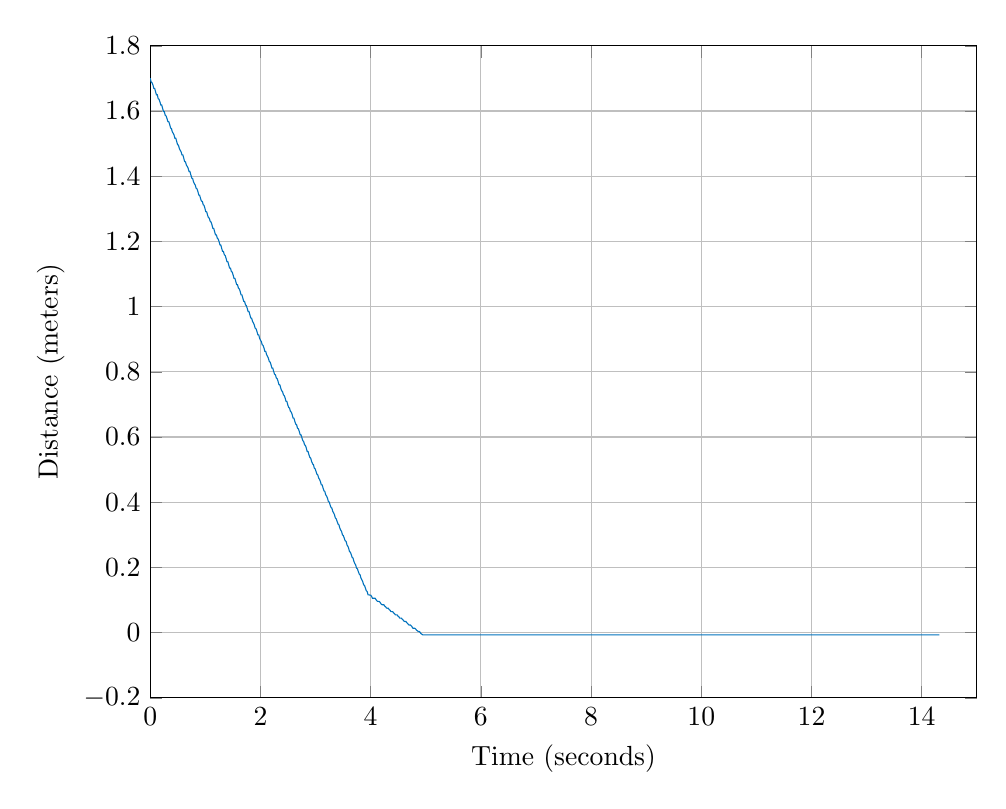
\begin{tikzpicture}

\begin{axis}[%
width=4.133in,
height=3.26in,
at={(0.693in,0.44in)},
scale only axis,
xmin=0,
xmax=15,
xmajorgrids,
xlabel={Time (seconds)},
ymin=-0.2,
ymax=1.8,
ymajorgrids,
ylabel={Distance (meters)},
axis background/.style={fill=white}
]
\addplot [color=mycolor1,solid,forget plot]
  table[row sep=crcr]{%
0	1.70070323259938\\
0.016069324000001	1.68890707061497\\
0.0320065329999998	1.68694606359605\\
0.0502430760000013	1.67910837211382\\
0.0654603220000006	1.66931033724084\\
0.0805304090000018	1.66931036116917\\
0.0961679069989994	1.65951260472534\\
0.112137013	1.64971500132616\\
0.128083598999001	1.64971558383299\\
0.144132344	1.63791561014145\\
0.160191256000001	1.63595515745871\\
0.176157670000002	1.62811805526458\\
0.192194776999	1.61832087273404\\
0.208126166000001	1.61832089727939\\
0.224266963998001	1.608523995145\\
0.240174423	1.59872753768209\\
0.256135519000001	1.59791450466272\\
0.272153828999002	1.58692473979563\\
0.288169008000001	1.58496414042135\\
0.304012991999999	1.57712787827488\\
0.320137411998998	1.56733159201528\\
0.336165612	1.56733168243909\\
0.354695472001001	1.55753578641125\\
0.369972818999998	1.5477398507696\\
0.38512234	1.54612607224657\\
0.400326026999999	1.53593364511751\\
0.416115708999999	1.53201556569763\\
0.432069677999999	1.52613791079744\\
0.448089598000001	1.51634260617269\\
0.464163109000001	1.51634266147623\\
0.480107651000001	1.50654766387199\\
0.496109260000002	1.4967528906098\\
0.512147802000001	1.49513558040406\\
0.528123054000001	1.48494323626048\\
0.544093956999999	1.4790674820486\\
0.559984897998001	1.47514834485282\\
0.575956071998998	1.4653538146669\\
0.592119272	1.46535399643784\\
0.608087780000001	1.4555598921508\\
0.624236109999999	1.44494772987982\\
0.640116497000001	1.44374680091474\\
0.656140651000001	1.43395285159923\\
0.672135993999999	1.43003547645872\\
0.688221121998999	1.42415897767332\\
0.704187274	1.41436543329959\\
0.72011518	1.41436552557409\\
0.736151451000001	1.40457257463715\\
0.754584281001002	1.39395969066141\\
0.769828182	1.392756196774\\
0.785160017000001	1.38296280254604\\
0.800265901000001	1.37708606976871\\
0.816153912	1.37317000483193\\
0.832145903000001	1.36337743391526\\
0.848135805998001	1.36141817534926\\
0.864115772	1.35358523727338\\
0.880153269001	1.34256687435143\\
0.896149572000001	1.34176548611479\\
0.912137691	1.33197334498306\\
0.928097120999999	1.3241385194695\\
0.946348925000001	1.32218136376134\\
0.961346119998999	1.31238972255499\\
0.976354984999999	1.3104305018962\\
0.992064543000001	1.30177556187101\\
1.008006571	1.29117634908583\\
1.024030649001	1.2907755610865\\
1.040145824	1.28098407253559\\
1.056120907	1.27315002301298\\
1.072136837	1.27119309119484\\
1.088177157	1.26140253455124\\
1.104091894	1.25944352455027\\
1.120102557	1.25078723802962\\
1.136188901	1.24018738746649\\
1.152242181	1.23978567753025\\
1.168036258	1.22999535825216\\
1.184091402999	1.22020513412421\\
1.200204026	1.22020530204309\\
1.216113982	1.21041548539911\\
1.232041107999	1.20763043320005\\
1.248098365	1.19979984044989\\
1.265526574	1.1891990365589\\
1.280866285	1.18879653878647\\
1.296088645	1.17900698822062\\
1.31214592	1.16921783692219\\
1.328065168	1.16921783692219\\
1.344105920001	1.15942922462601\\
1.360157336	1.15664267637973\\
1.376087194	1.14840437854889\\
1.392150168	1.13780760814362\\
1.408095583	1.13780760814362\\
1.42420924	1.12801912438761\\
1.440008907	1.11823102549804\\
1.456121564	1.11823102549804\\
1.472068705	1.10761344907527\\
1.488177739	1.10565502370803\\
1.504007510001	1.09701138411114\\
1.520113998	1.08681936285534\\
1.536127843	1.08681936285534\\
1.552444234	1.07703178258098\\
1.568079888	1.06724447499236\\
1.584153789	1.06724447499236\\
1.600215518	1.05662653405556\\
1.616091257	1.05425848582822\\
1.632872338998	1.04602345832516\\
1.648172934	1.03583151093506\\
1.664171419	1.03583159123549\\
1.680072930998	1.0260448763681\\
1.696169192	1.01625876710321\\
1.71210459	1.01584191946485\\
1.728066122	1.00563962813502\\
1.744099419	1.00327140446739\\
1.760177246999	0.994630225620793\\
1.776095221	0.984844266272094\\
1.792124911	0.984844429109161\\
1.808101937999	0.975058688593922\\
1.824180761	0.965273238381173\\
1.84011406	0.964439047203503\\
1.856080788	0.95465389227594\\
1.872133671	0.950326323463326\\
1.888252458999	0.943642659765013\\
1.904119091	0.933857618882051\\
1.920091132	0.931899888277566\\
1.936107338	0.924072847169644\\
1.953498289	0.913452674941421\\
1.968430135	0.913452630988693\\
1.983947726001	0.903256005818353\\
2.000004395999	0.896975855860554\\
2.016055560999	0.892655573028521\\
2.032046824	0.88287148201287\\
2.048082831	0.880914186043383\\
2.064106222	0.873087939233903\\
2.080208173	0.862466568456966\\
2.096084099999	0.862467190904421\\
2.112170826	0.852270550252034\\
2.128118515999	0.847537164752714\\
2.144126173	0.841669370495925\\
2.160102904	0.831886164959104\\
2.176107920001	0.829928864147527\\
2.192125173	0.821264318054896\\
2.208160362	0.811481738532172\\
2.224208805	0.811067994064579\\
2.240117272	0.800874882211913\\
2.256109963998	0.792638725384119\\
2.272122792001	0.790683634193174\\
2.288206	0.780901243050734\\
2.304158355999	0.778944564278034\\
2.320112761	0.770278897378079\\
2.336255208	0.76049686848324\\
2.352523716	0.760082956093384\\
2.368137319	0.749889832742865\\
2.38409622	0.741653421356722\\
2.400160084	0.739698759081924\\
2.416122277	0.729917382137484\\
2.432080348999	0.727117949314669\\
2.448060645999	0.719294131053078\\
2.464063677	0.709513519826042\\
2.480109089	0.709098148171513\\
2.496139034999	0.698494727247901\\
2.512176149	0.690669001241069\\
2.528096947999	0.688714359280124\\
2.544104168	0.678511473951389\\
2.560184079	0.676133471539559\\
2.576137217	0.668310206565276\\
2.59215698	0.658113828564659\\
2.608193492	0.657701571316304\\
2.624082607	0.647510152909211\\
2.640117643	0.639685061749649\\
2.656143765999	0.637731061940275\\
2.672172086999	0.627105905508042\\
2.688237514	0.62514910374261\\
2.704175049	0.617327445773804\\
2.720201493	0.607131062758107\\
2.736221201999	0.606717484950712\\
2.754618682	0.596526566048789\\
2.769783284	0.588702273181571\\
2.784850343999	0.585900741999466\\
2.800125557	0.576122405209377\\
2.816191003	0.574166280257926\\
2.832230402	0.565926694357188\\
2.848093178	0.555733971955455\\
2.864104655	0.555321220469471\\
2.880077262	0.54554344177775\\
2.896170501999	0.537720083689643\\
2.912105935	0.534917442609657\\
2.928051401	0.525139843781878\\
2.949731216	0.516898034933682\\
2.962121458	0.514944638236233\\
2.977390493	0.504752079008393\\
2.992827074	0.502381595227953\\
3.008384149	0.494561608987797\\
3.024476493	0.48588835800077\\
3.040135975	0.483934296503346\\
3.056209927	0.474158582752386\\
3.072150025	0.469826269067521\\
3.088250306	0.463546465815403\\
3.104166727	0.453355675355642\\
3.120123982999	0.453355911432862\\
3.136184394001	0.443153659078062\\
3.152213668001	0.43490622718137\\
3.168235699	0.432952826808204\\
3.184087276	0.422756897906481\\
3.200100611001	0.418844452951239\\
3.21614253	0.412565240163762\\
3.232182163	0.402374273123772\\
3.248129964	0.400418268698503\\
3.264190402	0.391746281275412\\
3.280159288001	0.383925114588184\\
3.296175784999	0.381971321362021\\
3.312171112999	0.371776518111717\\
3.328113913	0.367446924515144\\
3.343932748	0.361167705512951\\
3.359961541	0.351394151949116\\
3.376101852	0.348583175499767\\
3.392117823	0.340764711487065\\
3.408129227999	0.332945376318259\\
3.424172565	0.330569839956898\\
3.440076429	0.320796116638916\\
3.456144249	0.314511499387262\\
3.472144699	0.310187436355821\\
3.488191875	0.299985451203528\\
3.504106174	0.297602059624545\\
3.52019951	0.289785059387538\\
3.53607439	0.281965469016322\\
3.554542404999	0.279589399939724\\
3.569931210001	0.269398189396088\\
3.585245631999	0.265069091337944\\
3.600355143	0.259207494437546\\
3.616115829999	0.24857757462071\\
3.632199562999	0.24662236631056\\
3.648107895	0.238805280424047\\
3.664216821	0.230564138058408\\
3.680193602	0.228610943534281\\
3.696093144	0.218418917454134\\
3.712116623	0.212135795916174\\
3.728137332	0.207369367922327\\
3.744083689	0.197597791578987\\
3.760188013999	0.195643266023871\\
3.776096526	0.18740340476505\\
3.792296115	0.179585402876751\\
3.808094850999	0.177212138943696\\
3.824128024	0.167021781935662\\
3.840098481	0.162250074628208\\
3.856107515999	0.156389598061331\\
3.872126834	0.146620204136941\\
3.888159666999	0.144665477785741\\
3.904069126	0.136424841573279\\
3.920102831	0.128608927892266\\
3.936112366999	0.126234628800758\\
3.953593414999	0.115611890040436\\
3.968842935	0.115611890040436\\
3.984078578	0.115180714935151\\
4.000142381	0.115180714935151\\
4.016401236999	0.111270462418884\\
4.032133757	0.105410435235105\\
4.048164163	0.105410435235105\\
4.064115562	0.105410435235105\\
4.080283927	0.105410435235105\\
4.096205703999	0.101500182718838\\
4.112094426	0.0975931245641481\\
4.128080843999	0.0956401555350588\\
4.143969165	0.0956401555350588\\
4.160151095999	0.0952147768949405\\
4.176062444	0.0913045243786732\\
4.192102083	0.087397466223984\\
4.208085109	0.0854444971948947\\
4.224097702	0.0854444971948947\\
4.240026942999	0.0854444971948947\\
4.256114998999	0.0811122774764725\\
4.272170062	0.0791580377233891\\
4.288184549	0.0752522502926936\\
4.304157742	0.0748316480262143\\
4.32012377	0.0748316480262143\\
4.336112533	0.0704895387161499\\
4.353068628	0.0685352989630665\\
4.368398333999	0.0641983364270864\\
4.384091347	0.0641983364270864\\
4.400141004	0.0641983364270864\\
4.416222126	0.0602880839108195\\
4.432106447999	0.0583338441577359\\
4.448091508999	0.0544280567270401\\
4.464175883999	0.0544280567270401\\
4.480154263999	0.0544280567270401\\
4.496132243	0.0505178042107728\\
4.512113087	0.0485635644576894\\
4.528102168	0.044232398386876\\
4.544123569	0.044232398386876\\
4.560138824	0.044232398386876\\
4.576111998	0.0403221458706087\\
4.592154613	0.0383679061175253\\
4.608100419	0.0344621186868297\\
4.624175578999	0.0340401514846749\\
4.640078227	0.0340401514846749\\
4.656123298	0.0301298989684078\\
4.672069312	0.0277550569488449\\
4.68819105	0.0238492695181494\\
4.704105525	0.0234174127243527\\
4.720085222999	0.0234174127243527\\
4.736113877	0.0210312584170544\\
4.752566852999	0.0171217453497177\\
4.76814402	0.0132159579190219\\
4.784091632999	0.0132159579190219\\
4.80013614	0.0132159579190219\\
4.816126581	0.0112609787170082\\
4.832086137999	0.00735146564967115\\
4.848131159	0.00539864724806516\\
4.864128998001	0.00344567821897557\\
4.880645107	0.00344567821897557\\
4.896177155	0.00106532037684404\\
4.912115013999	-0.00284419269049296\\
4.928079191	-0.0047970110920994\\
4.946479170999	-0.00674998012118877\\
4.96177009	-0.00674998012118877\\
4.976940850999	-0.00674998012118877\\
4.992198873999	-0.00674998012118877\\
5.008107431	-0.00674998012118877\\
5.024180013999	-0.00674998012118877\\
5.040113272	-0.00674998012118877\\
5.056091562	-0.00674998012118877\\
5.072107562	-0.00674998012118877\\
5.088149657	-0.00674998012118877\\
5.104146225	-0.00674998012118877\\
5.120122668	-0.00674998012118877\\
5.136131117	-0.00674998012118877\\
5.152495065	-0.00674998012118877\\
5.168157123999	-0.00674998012118877\\
5.184086692999	-0.00674998012118877\\
5.20012561	-0.00674998012118877\\
5.216162032	-0.00674998012118877\\
5.232407311	-0.00674998012118877\\
5.248143728	-0.00674998012118877\\
5.264158846	-0.00674998012118877\\
5.280334113	-0.00674998012118877\\
5.296138749	-0.00674998012118877\\
5.312127127	-0.00674998012118877\\
5.328046558	-0.00674998012118877\\
5.344069329	-0.00674998012118877\\
5.360154541	-0.00674998012118877\\
5.376083287	-0.00674998012118877\\
5.392092152999	-0.00674998012118877\\
5.408073269	-0.00674998012118877\\
5.424094772	-0.00674998012118877\\
5.440135408	-0.00674998012118877\\
5.45611251	-0.00674998012118877\\
5.472117911	-0.00674998012118877\\
5.488166234999	-0.00674998012118877\\
5.504088559	-0.00674998012118877\\
5.520139673	-0.00674998012118877\\
5.536131288001	-0.00674998012118877\\
5.552530546	-0.00674998012118877\\
5.568152489	-0.00674998012118877\\
5.584304828	-0.00674998012118877\\
5.600132832	-0.00674998012118877\\
5.616125053999	-0.00674998012118877\\
5.63222296	-0.00674998012118877\\
5.648141236	-0.00674998012118877\\
5.664101102999	-0.00674998012118877\\
5.68007525	-0.00674998012118877\\
5.696140001999	-0.00674998012118877\\
5.712139545	-0.00674998012118877\\
5.7280556	-0.00674998012118877\\
5.744114973	-0.00674998012118877\\
5.7600981	-0.00674998012118877\\
5.776079805998	-0.00674998012118877\\
5.792099455	-0.00674998012118877\\
5.808099073	-0.00674998012118877\\
5.824111225	-0.00674998012118877\\
5.840144294	-0.00674998012118877\\
5.856088231	-0.00674998012118877\\
5.872113081	-0.00674998012118877\\
5.888200964	-0.00674998012118877\\
5.904104276	-0.00674998012118877\\
5.920123937999	-0.00674998012118877\\
5.936105710001	-0.00674998012118877\\
5.954122822999	-0.00674998012118877\\
5.969604967999	-0.00674998012118877\\
5.984906962	-0.00674998012118877\\
6.000129946	-0.00674998012118877\\
6.016174555998	-0.00674998012118877\\
6.032179637	-0.00674998012118877\\
6.04817237	-0.00674998012118877\\
6.06396628	-0.00674998012118877\\
6.08011849	-0.00674998012118877\\
6.096164213	-0.00674998012118877\\
6.112161556	-0.00674998012118877\\
6.12807971	-0.00674998012118877\\
6.144091369999	-0.00674998012118877\\
6.160147751999	-0.00674998012118877\\
6.176139043999	-0.00674998012118877\\
6.192096644	-0.00674998012118877\\
6.208063027	-0.00674998012118877\\
6.224189092	-0.00674998012118877\\
6.240115954999	-0.00674998012118877\\
6.256148949	-0.00674998012118877\\
6.272131335	-0.00674998012118877\\
6.288296085	-0.00674998012118877\\
6.304145408	-0.00674998012118877\\
6.320100149	-0.00674998012118877\\
6.336161968	-0.00674998012118877\\
6.352387193	-0.00674998012118877\\
6.368124876999	-0.00674998012118877\\
6.384090609	-0.00674998012118877\\
6.400211477	-0.00674998012118877\\
6.416132897	-0.00674998012118877\\
6.43216302	-0.00674998012118877\\
6.448151071999	-0.00674998012118877\\
6.464145046999	-0.00674998012118877\\
6.480096687	-0.00674998012118877\\
6.496158961999	-0.00674998012118877\\
6.512109579	-0.00674998012118877\\
6.528136283	-0.00674998012118877\\
6.544122510999	-0.00674998012118877\\
6.560145808	-0.00674998012118877\\
6.576076338	-0.00674998012118877\\
6.592102357999	-0.00674998012118877\\
6.608110555	-0.00674998012118877\\
6.624157255	-0.00674998012118877\\
6.640144956	-0.00674998012118877\\
6.656110868	-0.00674998012118877\\
6.67211425	-0.00674998012118877\\
6.688157572	-0.00674998012118877\\
6.70417262	-0.00674998012118877\\
6.720183333	-0.00674998012118877\\
6.736108498	-0.00674998012118877\\
6.752245251999	-0.00674998012118877\\
6.768170006	-0.00674998012118877\\
6.78409308	-0.00674998012118877\\
6.800121067	-0.00674998012118877\\
6.816309199	-0.00674998012118877\\
6.83214064	-0.00674998012118877\\
6.84816458	-0.00674998012118877\\
6.864047207	-0.00674998012118877\\
6.882458893	-0.00674998012118877\\
6.898193426	-0.00674998012118877\\
6.913355201	-0.00674998012118877\\
6.928491438	-0.00674998012118877\\
6.947047286999	-0.00674998012118877\\
6.962191612999	-0.00674998012118877\\
6.97749268	-0.00674998012118877\\
6.992973411999	-0.00674998012118877\\
7.008187886	-0.00674998012118877\\
7.024307571001	-0.00674998012118877\\
7.040167512999	-0.00674998012118877\\
7.056193491	-0.00674998012118877\\
7.072181076	-0.00674998012118877\\
7.088051545	-0.00674998012118877\\
7.10411717	-0.00674998012118877\\
7.1201266	-0.00674998012118877\\
7.136147	-0.00674998012118877\\
7.152521743	-0.00674998012118877\\
7.168185244999	-0.00674998012118877\\
7.184378821	-0.00674998012118877\\
7.20020143	-0.00674998012118877\\
7.216184781999	-0.00674998012118877\\
7.232042746	-0.00674998012118877\\
7.248120158	-0.00674998012118877\\
7.264152282	-0.00674998012118877\\
7.280110601001	-0.00674998012118877\\
7.296077453	-0.00674998012118877\\
7.312116305	-0.00674998012118877\\
7.328062463	-0.00674998012118877\\
7.344082802999	-0.00674998012118877\\
7.360174107999	-0.00674998012118877\\
7.37611575	-0.00674998012118877\\
7.392128623	-0.00674998012118877\\
7.408072085	-0.00674998012118877\\
7.424139204999	-0.00674998012118877\\
7.440146526	-0.00674998012118877\\
7.456088703999	-0.00674998012118877\\
7.472038822999	-0.00674998012118877\\
7.488180053999	-0.00674998012118877\\
7.504060756999	-0.00674998012118877\\
7.520148406	-0.00674998012118877\\
7.536141824999	-0.00674998012118877\\
7.552118135	-0.00674998012118877\\
7.568045088	-0.00674998012118877\\
7.584103691	-0.00674998012118877\\
7.600100111	-0.00674998012118877\\
7.616084619	-0.00674998012118877\\
7.632096045999	-0.00674998012118877\\
7.648137428	-0.00674998012118877\\
7.664059868	-0.00674998012118877\\
7.680081336999	-0.00674998012118877\\
7.696130774999	-0.00674998012118877\\
7.712076972001	-0.00674998012118877\\
7.728050767	-0.00674998012118877\\
7.744136119	-0.00674998012118877\\
7.760158163	-0.00674998012118877\\
7.776119765	-0.00674998012118877\\
7.792147027999	-0.00674998012118877\\
7.808121662	-0.00674998012118877\\
7.824165054	-0.00674998012118877\\
7.84012768	-0.00674998012118877\\
7.856007022	-0.00674998012118877\\
7.87211373	-0.00674998012118877\\
7.888178381	-0.00674998012118877\\
7.904130987	-0.00674998012118877\\
7.920069859999	-0.00674998012118877\\
7.936139731	-0.00674998012118877\\
7.953775329999	-0.00674998012118877\\
7.969668032	-0.00674998012118877\\
7.985027403	-0.00674998012118877\\
8.000271054	-0.00674998012118877\\
8.01623539	-0.00674998012118877\\
8.032170656	-0.00674998012118877\\
8.048092836999	-0.00674998012118877\\
8.064116625	-0.00674998012118877\\
8.080185134001	-0.00674998012118877\\
8.096545704999	-0.00674998012118877\\
8.112141948	-0.00674998012118877\\
8.128089786	-0.00674998012118877\\
8.144130993	-0.00674998012118877\\
8.160172759001	-0.00674998012118877\\
8.17604269	-0.00674998012118877\\
8.192096532	-0.00674998012118877\\
8.20813131	-0.00674998012118877\\
8.224284324999	-0.00674998012118877\\
8.240130847	-0.00674998012118877\\
8.256169037	-0.00674998012118877\\
8.272126705999	-0.00674998012118877\\
8.288162924	-0.00674998012118877\\
8.304089001	-0.00674998012118877\\
8.320118654	-0.00674998012118877\\
8.336111407	-0.00674998012118877\\
8.35222381	-0.00674998012118877\\
8.36800367	-0.00674998012118877\\
8.384124836999	-0.00674998012118877\\
8.400150532	-0.00674998012118877\\
8.416038322999	-0.00674998012118877\\
8.432180963	-0.00674998012118877\\
8.448114382	-0.00674998012118877\\
8.464116832	-0.00674998012118877\\
8.480201758	-0.00674998012118877\\
8.496179562	-0.00674998012118877\\
8.5121461	-0.00674998012118877\\
8.528064569	-0.00674998012118877\\
8.544117057	-0.00674998012118877\\
8.560155984	-0.00674998012118877\\
8.576152094	-0.00674998012118877\\
8.592142105999	-0.00674998012118877\\
8.608094496999	-0.00674998012118877\\
8.624191435	-0.00674998012118877\\
8.640126451	-0.00674998012118877\\
8.65613519	-0.00674998012118877\\
8.672107302	-0.00674998012118877\\
8.688176197	-0.00674998012118877\\
8.704124789999	-0.00674998012118877\\
8.720109309	-0.00674998012118877\\
8.736180685	-0.00674998012118877\\
8.754722136	-0.00674998012118877\\
8.77004038	-0.00674998012118877\\
8.785317873	-0.00674998012118877\\
8.800500435	-0.00674998012118877\\
8.81609285	-0.00674998012118877\\
8.832122011	-0.00674998012118877\\
8.848119418	-0.00674998012118877\\
8.864077602999	-0.00674998012118877\\
8.880198916999	-0.00674998012118877\\
8.896149854999	-0.00674998012118877\\
8.914511889999	-0.00674998012118877\\
8.929824631	-0.00674998012118877\\
8.950692117	-0.00674998012118877\\
8.960096365	-0.00674998012118877\\
8.976146439	-0.00674998012118877\\
8.992143906	-0.00674998012118877\\
9.008117805	-0.00674998012118877\\
9.024114022	-0.00674998012118877\\
9.040060557	-0.00674998012118877\\
9.056103355	-0.00674998012118877\\
9.072095720999	-0.00674998012118877\\
9.088147723	-0.00674998012118877\\
9.104121307	-0.00674998012118877\\
9.12006106	-0.00674998012118877\\
9.135977095999	-0.00674998012118877\\
9.154252893	-0.00674998012118877\\
9.169452529	-0.00674998012118877\\
9.184654485	-0.00674998012118877\\
9.200110902999	-0.00674998012118877\\
9.216127065	-0.00674998012118877\\
9.2321499	-0.00674998012118877\\
9.248116839	-0.00674998012118877\\
9.264138461999	-0.00674998012118877\\
9.280185794	-0.00674998012118877\\
9.296171635	-0.00674998012118877\\
9.312130315	-0.00674998012118877\\
9.328098151	-0.00674998012118877\\
9.344142019999	-0.00674998012118877\\
9.360185808	-0.00674998012118877\\
9.376069623999	-0.00674998012118877\\
9.392053430998	-0.00674998012118877\\
9.408120602	-0.00674998012118877\\
9.424209658	-0.00674998012118877\\
9.440149842	-0.00674998012118877\\
9.456218291	-0.00674998012118877\\
9.472129418	-0.00674998012118877\\
9.488248661999	-0.00674998012118877\\
9.504131387	-0.00674998012118877\\
9.519952980999	-0.00674998012118877\\
9.538157447999	-0.00674998012118877\\
9.553431193	-0.00674998012118877\\
9.568611835001	-0.00674998012118877\\
9.584108379	-0.00674998012118877\\
9.60014434	-0.00674998012118877\\
9.616132607	-0.00674998012118877\\
9.632131192999	-0.00674998012118877\\
9.648120251999	-0.00674998012118877\\
9.66413114	-0.00674998012118877\\
9.680548475	-0.00674998012118877\\
9.696041631	-0.00674998012118877\\
9.712112135	-0.00674998012118877\\
9.728083027999	-0.00674998012118877\\
9.7441133	-0.00674998012118877\\
9.760140866999	-0.00674998012118877\\
9.77593967	-0.00674998012118877\\
9.794039083	-0.00674998012118877\\
9.809258961999	-0.00674998012118877\\
9.824620905	-0.00674998012118877\\
9.840144079	-0.00674998012118877\\
9.856151941	-0.00674998012118877\\
9.872194115	-0.00674998012118877\\
9.888170663	-0.00674998012118877\\
9.904061769	-0.00674998012118877\\
9.920081488	-0.00674998012118877\\
9.936113198	-0.00674998012118877\\
9.953652331	-0.00674998012118877\\
9.968924142999	-0.00674998012118877\\
9.984063593	-0.00674998012118877\\
10.000176352999	-0.00674998012118877\\
10.016040633999	-0.00674998012118877\\
10.034296292001	-0.00674998012118877\\
10.049636953999	-0.00674998012118877\\
10.064812324	-0.00674998012118877\\
10.080188750999	-0.00674998012118877\\
10.096130879	-0.00674998012118877\\
10.112182079	-0.00674998012118877\\
10.12808363	-0.00674998012118877\\
10.144123463998	-0.00674998012118877\\
10.160217276	-0.00674998012118877\\
10.176151546	-0.00674998012118877\\
10.192125992	-0.00674998012118877\\
10.208091071999	-0.00674998012118877\\
10.22422018	-0.00674998012118877\\
10.240147147	-0.00674998012118877\\
10.256122239	-0.00674998012118877\\
10.272144389	-0.00674998012118877\\
10.288190722	-0.00674998012118877\\
10.304097590999	-0.00674998012118877\\
10.320097038	-0.00674998012118877\\
10.336114321001	-0.00674998012118877\\
10.35444728	-0.00674998012118877\\
10.36960449	-0.00674998012118877\\
10.384746942	-0.00674998012118877\\
10.400098682	-0.00674998012118877\\
10.416172654	-0.00674998012118877\\
10.432186895	-0.00674998012118877\\
10.448177332	-0.00674998012118877\\
10.464142697999	-0.00674998012118877\\
10.480176559	-0.00674998012118877\\
10.49621088	-0.00674998012118877\\
10.512143341	-0.00674998012118877\\
10.528178725999	-0.00674998012118877\\
10.544110693	-0.00674998012118877\\
10.560157234999	-0.00674998012118877\\
10.576150479	-0.00674998012118877\\
10.592121763	-0.00674998012118877\\
10.608206599	-0.00674998012118877\\
10.624184447999	-0.00674998012118877\\
10.640245806	-0.00674998012118877\\
10.656904711999	-0.00674998012118877\\
10.672101326999	-0.00674998012118877\\
10.688143823	-0.00674998012118877\\
10.704209294	-0.00674998012118877\\
10.720099525	-0.00674998012118877\\
10.736090037	-0.00674998012118877\\
10.754553145999	-0.00674998012118877\\
10.769715192	-0.00674998012118877\\
10.784837237	-0.00674998012118877\\
10.800131693	-0.00674998012118877\\
10.816096171	-0.00674998012118877\\
10.8321314	-0.00674998012118877\\
10.848120603	-0.00674998012118877\\
10.864085819999	-0.00674998012118877\\
10.880158819	-0.00674998012118877\\
10.896102405	-0.00674998012118877\\
10.912232269	-0.00674998012118877\\
10.928119377	-0.00674998012118877\\
10.947387499	-0.00674998012118877\\
10.960121168999	-0.00674998012118877\\
10.976016628999	-0.00674998012118877\\
10.992141934	-0.00674998012118877\\
11.008090647	-0.00674998012118877\\
11.024145081	-0.00674998012118877\\
11.040162037	-0.00674998012118877\\
11.056084128999	-0.00674998012118877\\
11.07215134	-0.00674998012118877\\
11.088190498	-0.00674998012118877\\
11.104144117	-0.00674998012118877\\
11.120102857999	-0.00674998012118877\\
11.136107202	-0.00674998012118877\\
11.154456222	-0.00674998012118877\\
11.169595251	-0.00674998012118877\\
11.184767975	-0.00674998012118877\\
11.200155978	-0.00674998012118877\\
11.216135085	-0.00674998012118877\\
11.232049645	-0.00674998012118877\\
11.248120244	-0.00674998012118877\\
11.264141982999	-0.00674998012118877\\
11.280007942999	-0.00674998012118877\\
11.298251744999	-0.00674998012118877\\
11.3133739	-0.00674998012118877\\
11.328647735	-0.00674998012118877\\
11.34409634	-0.00674998012118877\\
11.360170626999	-0.00674998012118877\\
11.376118503	-0.00674998012118877\\
11.392095003	-0.00674998012118877\\
11.408155224	-0.00674998012118877\\
11.424185884001	-0.00674998012118877\\
11.440118865	-0.00674998012118877\\
11.456066869999	-0.00674998012118877\\
11.472152479	-0.00674998012118877\\
11.48809469	-0.00674998012118877\\
11.504090848	-0.00674998012118877\\
11.520145395	-0.00674998012118877\\
11.536128053999	-0.00674998012118877\\
11.554640930998	-0.00674998012118877\\
11.569952855	-0.00674998012118877\\
11.585109124	-0.00674998012118877\\
11.600346395	-0.00674998012118877\\
11.616135702	-0.00674998012118877\\
11.631963001	-0.00674998012118877\\
11.647947741	-0.00674998012118877\\
11.663938923	-0.00674998012118877\\
11.680079929	-0.00674998012118877\\
11.696258369999	-0.00674998012118877\\
11.712115465	-0.00674998012118877\\
11.728085722	-0.00674998012118877\\
11.744085069	-0.00674998012118877\\
11.760164803999	-0.00674998012118877\\
11.776104036	-0.00674998012118877\\
11.792097595	-0.00674998012118877\\
11.808122225	-0.00674998012118877\\
11.824166895	-0.00674998012118877\\
11.840146888999	-0.00674998012118877\\
11.856115106	-0.00674998012118877\\
11.872132434	-0.00674998012118877\\
11.888080593999	-0.00674998012118877\\
11.904123532	-0.00674998012118877\\
11.920102488	-0.00674998012118877\\
11.936102155	-0.00674998012118877\\
11.95412596	-0.00674998012118877\\
11.969472970999	-0.00674998012118877\\
11.984763995	-0.00674998012118877\\
12.000124543	-0.00674998012118877\\
12.016118041999	-0.00674998012118877\\
12.032157979	-0.00674998012118877\\
12.048179168999	-0.00674998012118877\\
12.063959744999	-0.00674998012118877\\
12.082052449999	-0.00674998012118877\\
12.09607277	-0.00674998012118877\\
12.11210849	-0.00674998012118877\\
12.128129116	-0.00674998012118877\\
12.144084538999	-0.00674998012118877\\
12.160176581	-0.00674998012118877\\
12.176088244999	-0.00674998012118877\\
12.192203411999	-0.00674998012118877\\
12.20814622	-0.00674998012118877\\
12.224208658	-0.00674998012118877\\
12.240166456	-0.00674998012118877\\
12.256101074	-0.00674998012118877\\
12.271945064	-0.00674998012118877\\
12.290198464	-0.00674998012118877\\
12.305413154	-0.00674998012118877\\
12.320627012	-0.00674998012118877\\
12.336102488	-0.00674998012118877\\
12.354440303	-0.00674998012118877\\
12.369604072999	-0.00674998012118877\\
12.384668447	-0.00674998012118877\\
12.400073527999	-0.00674998012118877\\
12.416234076	-0.00674998012118877\\
12.432129102	-0.00674998012118877\\
12.448081057	-0.00674998012118877\\
12.46411798	-0.00674998012118877\\
12.480147645999	-0.00674998012118877\\
12.496145685999	-0.00674998012118877\\
12.512123956	-0.00674998012118877\\
12.527957866	-0.00674998012118877\\
12.544149948	-0.00674998012118877\\
12.56019972	-0.00674998012118877\\
12.576162607999	-0.00674998012118877\\
12.592128406001	-0.00674998012118877\\
12.608130044	-0.00674998012118877\\
12.624152102999	-0.00674998012118877\\
12.640100409	-0.00674998012118877\\
12.656106778	-0.00674998012118877\\
12.67214101	-0.00674998012118877\\
12.688148937	-0.00674998012118877\\
12.704122822	-0.00674998012118877\\
12.720140861	-0.00674998012118877\\
12.736107655	-0.00674998012118877\\
12.752610784	-0.00674998012118877\\
12.768254937999	-0.00674998012118877\\
12.784170293	-0.00674998012118877\\
12.800125685999	-0.00674998012118877\\
12.816036273	-0.00674998012118877\\
12.832133523	-0.00674998012118877\\
12.848121039	-0.00674998012118877\\
12.86418619	-0.00674998012118877\\
12.880116661999	-0.00674998012118877\\
12.896180501	-0.00674998012118877\\
12.912196522	-0.00674998012118877\\
12.928101921	-0.00674998012118877\\
12.946379994999	-0.00674998012118877\\
12.961683178	-0.00674998012118877\\
12.976902510999	-0.00674998012118877\\
12.992136339	-0.00674998012118877\\
13.008079968	-0.00674998012118877\\
13.023981913	-0.00674998012118877\\
13.040161644001	-0.00674998012118877\\
13.056137133	-0.00674998012118877\\
13.071922963	-0.00674998012118877\\
13.090298756999	-0.00674998012118877\\
13.105471848	-0.00674998012118877\\
13.120543359	-0.00674998012118877\\
13.136114912	-0.00674998012118877\\
13.154388842	-0.00674998012118877\\
13.169506772998	-0.00674998012118877\\
13.184573854001	-0.00674998012118877\\
13.200108735	-0.00674998012118877\\
13.216114081	-0.00674998012118877\\
13.232155317999	-0.00674998012118877\\
13.248075816	-0.00674998012118877\\
13.264070277999	-0.00674998012118877\\
13.28008042	-0.00674998012118877\\
13.296007821	-0.00674998012118877\\
13.311951169	-0.00674998012118877\\
13.327948697	-0.00674998012118877\\
13.344136313	-0.00674998012118877\\
13.360203449	-0.00674998012118877\\
13.376143522	-0.00674998012118877\\
13.392101085	-0.00674998012118877\\
13.408081495	-0.00674998012118877\\
13.42420339	-0.00674998012118877\\
13.440065956	-0.00674998012118877\\
13.45610049	-0.00674998012118877\\
13.472134952	-0.00674998012118877\\
13.488228749	-0.00674998012118877\\
13.504126025	-0.00674998012118877\\
13.519953545999	-0.00674998012118877\\
13.53811773	-0.00674998012118877\\
13.553443261	-0.00674998012118877\\
13.569039269	-0.00674998012118877\\
13.584445684	-0.00674998012118877\\
13.600127585001	-0.00674998012118877\\
13.61615575	-0.00674998012118877\\
13.632144334	-0.00674998012118877\\
13.648122689	-0.00674998012118877\\
13.664154639999	-0.00674998012118877\\
13.680109121	-0.00674998012118877\\
13.696166079	-0.00674998012118877\\
13.712085664999	-0.00674998012118877\\
13.728084994	-0.00674998012118877\\
13.744133387	-0.00674998012118877\\
13.760221902	-0.00674998012118877\\
13.776187319999	-0.00674998012118877\\
13.792134414	-0.00674998012118877\\
13.807975776	-0.00674998012118877\\
13.824156364	-0.00674998012118877\\
13.840071372	-0.00674998012118877\\
13.856145722999	-0.00674998012118877\\
13.872142354	-0.00674998012118877\\
13.888196796999	-0.00674998012118877\\
13.904183074999	-0.00674998012118877\\
13.920124682	-0.00674998012118877\\
13.93611789	-0.00674998012118877\\
13.954062112999	-0.00674998012118877\\
13.969419541999	-0.00674998012118877\\
13.984792093999	-0.00674998012118877\\
14.000132809999	-0.00674998012118877\\
14.016145808	-0.00674998012118877\\
14.032146192999	-0.00674998012118877\\
14.048147355	-0.00674998012118877\\
14.064136334	-0.00674998012118877\\
14.08006137	-0.00674998012118877\\
14.096279949	-0.00674998012118877\\
14.112124784999	-0.00674998012118877\\
14.127938703	-0.00674998012118877\\
14.145621328	-0.00674998012118877\\
14.161255758999	-0.00674998012118877\\
14.17655692	-0.00674998012118877\\
14.192112202	-0.00674998012118877\\
14.208086177	-0.00674998012118877\\
14.224163666999	-0.00674998012118877\\
14.240077209	-0.00674998012118877\\
14.256090142999	-0.00674998012118877\\
14.272144014	-0.00674998012118877\\
14.288091156001	-0.00674998012118877\\
14.304054423	-0.00674998012118877\\
14.320096062	-0.00674998012118877\\
};
\end{axis}
\end{tikzpicture}%
}
      \caption{The error in displacement of the robot over time for
        $(K_{\Psi}^R, K_{\omega}^T) \equiv (0.2 K_{\Psi, max}^R, 0.5 K_{\omega, max}^T)$}
      \label{fig:19_7_distance}
    \end{figure}
  \end{minipage}
  \hfill
  \begin{minipage}{0.45\linewidth}
    \begin{figure}[H]
      \scalebox{0.6}{% This file was created by matlab2tikz.
%
%The latest updates can be retrieved from
%  http://www.mathworks.com/matlabcentral/fileexchange/22022-matlab2tikz-matlab2tikz
%where you can also make suggestions and rate matlab2tikz.
%
\definecolor{mycolor1}{rgb}{0.00000,0.44700,0.74100}%
%
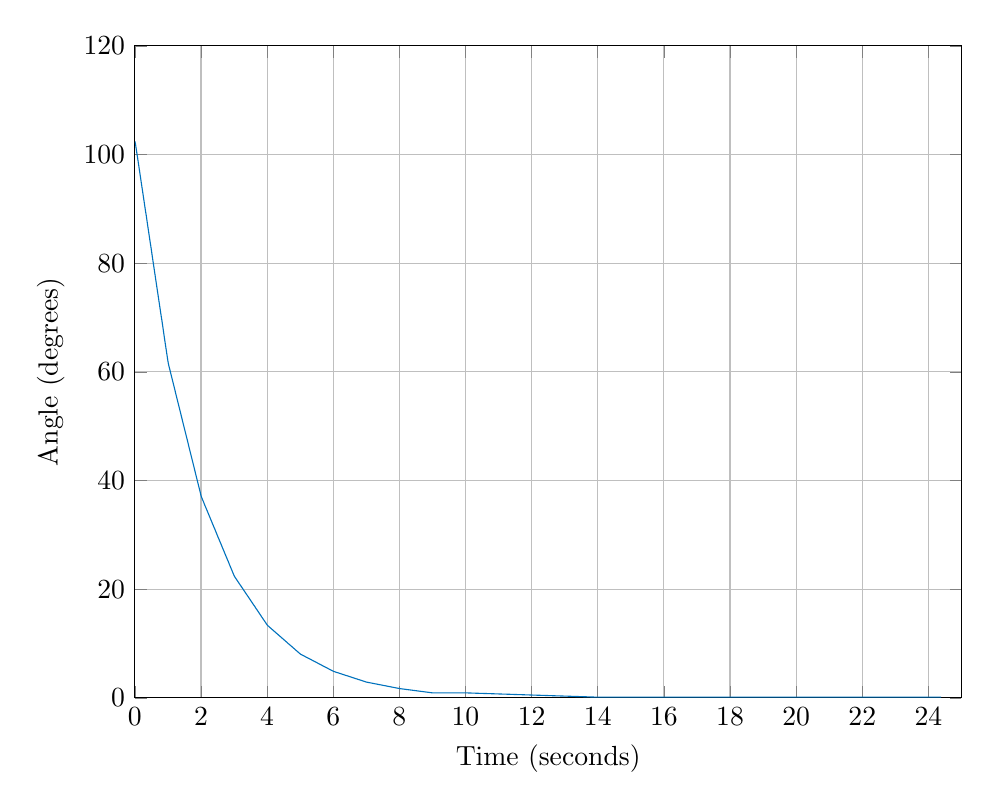
\begin{tikzpicture}

\begin{axis}[%
width=4.133in,
height=3.26in,
at={(0.693in,0.44in)},
scale only axis,
xmin=0,
xmax=25,
xmajorgrids,
xlabel={Time (seconds)},
ymin=0,
ymax=120,
ymajorgrids,
ylabel={Angle (degrees)},
axis background/.style={fill=white}
]
\addplot [color=mycolor1,solid,forget plot]
  table[row sep=crcr]{%
0	102.4204\\
0.017680273	102.0004\\
0.0326910660000006	101.3704\\
0.0478512429999998	100.7584\\
0.0638764890000001	100.1124\\
0.0799588490000004	99.4844\\
0.0958651979999999	98.8464\\
0.111923665	98.1924\\
0.127986862000001	97.5384\\
0.144054695	96.8864\\
0.159914538999001	96.2264\\
0.17601809	95.5744\\
0.191946917	94.8984\\
0.208079209999001	94.2544\\
0.223989928	93.6104\\
0.239952898001	92.9664\\
0.255942068	92.3044\\
0.271942981000001	91.6584\\
0.288054942	90.9744\\
0.303993131	90.3304\\
0.319898738999	89.6764\\
0.338376994001	89.0044\\
0.354037594000001	88.3544\\
0.369093324	87.7224\\
0.384204203999001	87.0784\\
0.399996272	86.4284\\
0.416472500000001	85.7724\\
0.431974013999999	85.1224\\
0.447922317000001	84.4724\\
0.463946346	83.8164\\
0.482375421999999	83.1344\\
0.497833884000001	82.4924\\
0.512944313	81.8424\\
0.528342609	81.1944\\
0.544029618999	80.5524\\
0.55995921	79.8904\\
0.576000115000001	79.2464\\
0.591977398000999	78.5924\\
0.607982704000001	77.9404\\
0.624034299001	77.2744\\
0.639961316000001	76.6284\\
0.655957358	75.9704\\
0.67193844	75.3244\\
0.688035293000001	74.6684\\
0.703973472	74.0204\\
0.719969571998999	73.3644\\
0.735977464000001	72.7164\\
0.752104601000001	72.0564\\
0.767968577	71.4084\\
0.783949898000001	70.7564\\
0.799954111999	70.0984\\
0.818500755	69.4184\\
0.834119084999	68.7704\\
0.849363261000001	68.1204\\
0.864831111	67.4744\\
0.880055500999001	66.8264\\
0.896061910000001	66.1524\\
0.911966587999	65.5044\\
0.927954776	64.8624\\
0.944057603000001	64.2164\\
0.960030365000999	63.5664\\
0.975909328000001	62.9164\\
0.991950462	62.2644\\
1.010365616	61.5944\\
1.025310158	61.1884\\
1.04021214	60.8244\\
1.055832138	60.4504\\
1.073996943	60.0144\\
1.089052950999	59.6364\\
1.104370401	59.2524\\
1.119958508	58.8724\\
1.136001529	58.4784\\
1.152015896	58.0864\\
1.168022066	57.6944\\
1.183979170999	57.3024\\
1.200197013	56.9104\\
1.216443756	56.5124\\
1.231977618999	56.1064\\
1.247982273999	55.7224\\
1.263959365999	55.3164\\
1.280113092999	54.9304\\
1.295911162	54.5424\\
1.31196283	54.1564\\
1.327985997	53.7644\\
1.343998571999	53.3704\\
1.360053891001	52.9784\\
1.376103250999	52.5784\\
1.391971526	52.1864\\
1.408042054	51.7924\\
1.423817408999	51.4024\\
1.439809614	51.0104\\
1.455967813	50.6164\\
1.471980966999	50.2224\\
1.488028499	49.8284\\
1.503919798	49.4384\\
1.519933752	49.0484\\
1.535969131	48.6344\\
1.552048325	48.2604\\
1.567808023	47.8664\\
1.586103383	47.4604\\
1.601386443	47.0604\\
1.616776504	46.6764\\
1.632014834	46.2744\\
1.648051942	45.8884\\
1.664009846	45.4804\\
1.679989383	45.0904\\
1.695928054	44.7044\\
1.711971441	44.3124\\
1.728026449	43.9284\\
1.744028953999	43.5424\\
1.759907247	43.1444\\
1.77599245	42.7524\\
1.791998698	42.3604\\
1.807958127	41.9664\\
1.824424295	41.5604\\
1.840004503	41.1724\\
1.855970019	40.7824\\
1.871964281	40.3964\\
1.88805972	39.9864\\
1.903980575	39.6004\\
1.920022889	39.2124\\
1.936062658999	38.8084\\
1.952027728	38.4184\\
1.967967882	38.0304\\
1.983977077	37.6424\\
1.999971243	37.2404\\
2.017336051	36.9164\\
2.032277945	36.6804\\
2.047807195999	36.4484\\
2.065928836	36.2124\\
2.080897507	35.9864\\
2.096205201	35.7464\\
2.111901924001	35.5064\\
2.127848016	35.2724\\
2.143809912	35.0444\\
2.159995884	34.8144\\
2.17596372	34.5824\\
2.191901353	34.3524\\
2.207950236999	34.1024\\
2.223912698998	33.8744\\
2.240004383	33.6444\\
2.256039261001	33.4084\\
2.271987563	33.1764\\
2.288045899	32.9384\\
2.303955608999	32.7004\\
2.319981065	32.4704\\
2.336020554	32.2384\\
2.352036599	31.9924\\
2.367874281	31.7604\\
2.384005412	31.5324\\
2.399965354999	31.2904\\
2.418337944	31.0504\\
2.433619645	30.8184\\
2.449024776999	30.5844\\
2.464310233	30.3464\\
2.480042389999	30.1144\\
2.495855733	29.8864\\
2.511935045	29.6224\\
2.52801317	29.4124\\
2.543960761	29.1824\\
2.560007551999	28.9464\\
2.577218852	28.7084\\
2.592363038999	28.4804\\
2.608537794	28.2444\\
2.623881354999	28.0044\\
2.639813344	27.7744\\
2.655850764999	27.5404\\
2.671970861	27.3124\\
2.688023389	27.0764\\
2.703962786	26.8344\\
2.719941531999	26.6004\\
2.736039162001	26.3704\\
2.752034645	26.1264\\
2.767942657	25.8964\\
2.783951590999	25.6684\\
2.799994156	25.4224\\
2.818564342	25.1864\\
2.833879976	24.9524\\
2.849187466	24.7104\\
2.864410158999	24.4784\\
2.879962665	24.2504\\
2.895990482	24.0204\\
2.911947939	23.7864\\
2.928026912	23.5564\\
2.94399345	23.3204\\
2.959999292999	23.0884\\
2.975969143	22.8524\\
2.99202088	22.6184\\
3.010108302	22.3764\\
3.025081368	22.2304\\
3.040024314	22.0924\\
3.055884978	21.9544\\
3.071866104	21.8084\\
3.087985985	21.6644\\
3.10395791	21.5204\\
3.119972738	21.3784\\
3.135995243	21.2264\\
3.151954971999	21.0824\\
3.167938511999	20.9424\\
3.183949997999	20.7884\\
3.199971265	20.6444\\
3.218263677	20.5004\\
3.23336733	20.3564\\
3.248597781999	20.2144\\
3.263968915	20.0704\\
3.279945408	19.9304\\
3.29597205	19.7844\\
3.311953953	19.6364\\
3.328072323	19.4884\\
3.343877074	19.3464\\
3.360006654	19.2044\\
3.376050434	19.0604\\
3.391988420999	18.9184\\
3.407798753	18.7724\\
3.426145757	18.6244\\
3.44128471	18.4804\\
3.456533712999	18.3304\\
3.471957927999	18.1904\\
3.488045224	18.0464\\
3.50391346	17.9084\\
3.519915404	17.7604\\
3.535963832	17.6184\\
3.552024943	17.4724\\
3.568132493	17.3284\\
3.584030009	17.1764\\
3.599975811	17.0324\\
3.618325011	16.8844\\
3.633464476	16.7444\\
3.648499299	16.6004\\
3.663966084999	16.4564\\
3.679974157	16.3144\\
3.695942165	16.1704\\
3.712072573	16.0204\\
3.728029519	15.8784\\
3.744047623999	15.7364\\
3.760059585	15.5924\\
3.775967145	15.4484\\
3.791942774	15.3004\\
3.807987033	15.1564\\
3.824035646999	15.0164\\
3.839955299001	14.8484\\
3.855974437	14.7244\\
3.871966052	14.5764\\
3.888030948	14.4324\\
3.903961064	14.2904\\
3.920075611999	14.1464\\
3.935961848	13.9984\\
3.952074383	13.8544\\
3.967997061001	13.7104\\
3.983976349	13.5584\\
4.00000613	13.4164\\
4.015872438	13.3044\\
4.031832225	13.2224\\
4.049913605	13.1344\\
4.064804169	13.0464\\
4.07987763	12.9684\\
4.09584957	12.8824\\
4.114056036	12.7904\\
4.129272264999	12.7084\\
4.144571130999	12.6244\\
4.160011762999	12.5384\\
4.175994698	12.4564\\
4.191933879001	12.3724\\
4.207940907	12.2844\\
4.224038089	12.2024\\
4.240056825001	12.1184\\
4.255865903999	12.0344\\
4.271971074	11.9444\\
4.288024008	11.8604\\
4.304003535001	11.7744\\
4.319970054	11.6944\\
4.335985147	11.6064\\
4.35202982	11.5204\\
4.367997512999	11.4384\\
4.383987785	11.3544\\
4.399978648	11.2684\\
4.418318467	11.1784\\
4.433488231	11.0944\\
4.448518077	11.0124\\
4.463987939999	10.9304\\
4.479970495	10.8424\\
4.495999996	10.7604\\
4.511970603	10.6744\\
4.528038135	10.5904\\
4.544318309	10.5024\\
4.559989568	10.4184\\
4.575995912	10.3344\\
4.591987616999	10.2484\\
4.607959491999	10.1624\\
4.624002057999	10.0804\\
4.639989243	9.97839999999999\\
4.655840926	9.90639999999999\\
4.672095316	9.82239999999999\\
4.688059544	9.7364\\
4.703974322	9.65439999999998\\
4.719973021	9.5684\\
4.736070792	9.4824\\
4.751991917	9.3984\\
4.767898045	9.31439999999999\\
4.78395887	9.2304\\
4.799973637999	9.14239999999999\\
4.818517439	9.0544\\
4.833979399	8.97240000000001\\
4.849021412999	8.8884\\
4.864259646	8.7984\\
4.879993102	8.71639999999999\\
4.895872277001	8.6324\\
4.911925215999	8.54839999999999\\
4.928029561	8.4644\\
4.944009736	8.37840000000001\\
4.959924648	8.2884\\
4.976017842999	8.20439999999999\\
4.991972156	8.1224\\
5.009711056	8.04040000000001\\
5.024677059999	7.98440000000001\\
5.039888167	7.93640000000001\\
5.055836128	7.88839999999999\\
5.073984147	7.83439999999999\\
5.089105106	7.78639999999999\\
5.104246502	7.73840000000001\\
5.119942608	7.6884\\
5.135985439	7.63839999999999\\
5.152059811	7.58439999999999\\
5.168003112	7.53239999999998\\
5.183949684999	7.4804\\
5.199980669	7.43039999999999\\
5.218391725	7.3784\\
5.233672379001	7.3304\\
5.248932587	7.27839999999999\\
5.26420111	7.22639999999998\\
5.280057373	7.1784\\
5.296098861	7.1284\\
5.311996974	7.0784\\
5.328238641	7.02839999999999\\
5.343935801	6.97839999999999\\
5.359932971	6.9264\\
5.376004527001	6.87440000000001\\
5.391930764	6.82239999999999\\
5.407952462999	6.7704\\
5.424028168	6.72039999999998\\
5.439934475	6.66839999999999\\
5.455980132	6.61840000000001\\
5.472032675	6.5684\\
5.489120174	6.51639999999999\\
5.504493998	6.46839999999999\\
5.519986061999	6.41839999999998\\
5.535995686999	6.3664\\
5.552017451	6.31639999999999\\
5.567910007	6.26839999999999\\
5.583986398	6.21439999999998\\
5.599969359	6.16439999999997\\
5.616024116999	6.11240000000001\\
5.631948084	6.06039999999999\\
5.64797575	6.01039999999999\\
5.663991946	5.9564\\
5.680180051	5.90639999999999\\
5.695920792	5.8584\\
5.712052385	5.80839999999999\\
5.727979985	5.75839999999999\\
5.744005250999	5.7084\\
5.760018601	5.65639999999999\\
5.776021130999	5.60640000000001\\
5.792059877	5.5564\\
5.807958893	5.5064\\
5.823871589	5.45239999999998\\
5.83994855	5.40239999999999\\
5.855890490999	5.35039999999999\\
5.871954158	5.2984\\
5.888019719999	5.2484\\
5.90396935	5.1964\\
5.919949099	5.1484\\
5.935963740999	5.09639999999999\\
5.951923957	5.04640000000001\\
5.967991507	4.99640000000001\\
5.983969887999	4.94839999999999\\
5.999963360999	4.89639999999999\\
6.017773040998	4.85239999999999\\
6.032762898	4.82239999999999\\
6.047836646	4.7924\\
6.065917793	4.75239999999999\\
6.080884396999	4.72239999999998\\
6.095976695	4.69239999999999\\
6.111942401999	4.66039999999998\\
6.127898505999	4.63039999999999\\
6.143983854	4.60039999999999\\
6.159943896999	4.5684\\
6.175984071999	4.53839999999998\\
6.191960864	4.5044\\
6.207946335	4.47239999999998\\
6.22404187	4.44239999999999\\
6.240049567	4.41039999999998\\
6.255975648001	4.3784\\
6.271952519999	4.3484\\
6.288057527001	4.31440000000001\\
6.303945808	4.28239999999998\\
6.319890820999	4.25239999999999\\
6.335964067	4.22039999999998\\
6.352061405	4.1884\\
6.368051208	4.15439999999998\\
6.383996943999	4.1224\\
6.399962766	4.09239999999998\\
6.418367762	4.0624\\
6.433704043	4.03039999999999\\
6.448817063	3.9984\\
6.463977054	3.96439999999998\\
6.479922316	3.9324\\
6.496090253	3.90239999999999\\
6.511901181999	3.8724\\
6.527948724	3.84039999999999\\
6.543927302999	3.8064\\
6.560014538	3.77439999999999\\
6.575998590999	3.74040000000001\\
6.591990330999	3.71039999999999\\
6.607993587999	3.68039999999999\\
6.624138575	3.65039999999999\\
6.639796391	3.61640000000001\\
6.655810885	3.58239999999999\\
6.671958775	3.55240000000001\\
6.687832245999	3.52239999999999\\
6.703879021	3.49040000000001\\
6.719814221	3.46039999999999\\
6.735799123999	3.42440000000001\\
6.752032636	3.39239999999998\\
6.767863095	3.3604\\
6.783961572	3.33239999999999\\
6.799961563	3.3004\\
6.818635384	3.2684\\
6.833845248	3.2364\\
6.848982192	3.20039999999999\\
6.864138651	3.1704\\
6.879969912	3.14039999999999\\
6.896009222	3.11240000000001\\
6.911965873999	3.0784\\
6.927976089001	3.04640000000001\\
6.943888625999	3.01239999999999\\
6.959959057999	2.9804\\
6.975996271	2.94839999999999\\
6.991965700999	2.91639999999998\\
7.010190373999	2.89039999999999\\
7.02516578	2.86840000000001\\
7.040083040998	2.8484\\
7.05587776	2.8284\\
7.074031006999	2.81039999999999\\
7.089241464	2.7924\\
7.104492828	2.77839999999999\\
7.120043349	2.75839999999999\\
7.136012433	2.7384\\
7.152147071999	2.71839999999999\\
7.167816743	2.69839999999999\\
7.18385141	2.6784\\
7.200009592999	2.65839999999999\\
7.216419971	2.64239999999999\\
7.231954049	2.6224\\
7.247955446999	2.60439999999998\\
7.263953702	2.58239999999999\\
7.279964825999	2.5684\\
7.296009366999	2.5484\\
7.311980358999	2.52839999999999\\
7.32812326	2.50839999999999\\
7.343945589	2.4884\\
7.359801431999	2.46839999999999\\
7.377894255	2.44839999999999\\
7.393848101	2.43039999999999\\
7.409007991	2.41239999999998\\
7.424261941	2.39439999999999\\
7.439904435001	2.3764\\
7.455958901999	2.35640000000001\\
7.471902821	2.33839999999999\\
7.487981717	2.3184\\
7.504003670999	2.2984\\
7.519833569	2.27839999999999\\
7.536008334	2.26039999999999\\
7.552069913	2.2424\\
7.567971815	2.22239999999999\\
7.583958428	2.20439999999999\\
7.599926762	2.18639999999999\\
7.615856231	2.16839999999999\\
7.631944563	2.1484\\
7.647822740999	2.1284\\
7.663805721	2.1084\\
7.679834907	2.08839999999999\\
7.69837175	2.0684\\
7.713655911	2.0504\\
7.728810811	2.03039999999999\\
7.744057228	2.01239999999999\\
7.759947962999	1.9944\\
7.77596421	1.97840000000001\\
7.791957849	1.9584\\
7.807935082	1.9384\\
7.824118280999	1.91839999999999\\
7.839977812	1.8984\\
7.855950714	1.8784\\
7.871981067	1.8604\\
7.887868691	1.84039999999999\\
7.903940070001	1.8244\\
7.919992939999	1.8044\\
7.936022527001	1.78639999999999\\
7.952053936999	1.7664\\
7.967946632	1.7484\\
7.983973629	1.72840000000001\\
7.999946742	1.7084\\
8.017470543	1.69239999999999\\
8.032472939	1.6784\\
8.047825929999	1.66839999999999\\
8.063806795	1.65439999999998\\
8.081990717	1.63839999999999\\
8.097125396	1.6284\\
8.112242545	1.61840000000001\\
8.127912986999	1.60439999999998\\
8.144102491	1.59039999999999\\
8.160020823998	1.5784\\
8.175969738	1.5664\\
8.192019203999	1.5544\\
8.207980415	1.53839999999998\\
8.223918835	1.52839999999999\\
8.239960939	1.5164\\
8.25594192	1.50239999999999\\
8.271940892	1.4884\\
8.288065453	1.47840000000001\\
8.303945736	1.46439999999998\\
8.319970536	1.4524\\
8.335964682	1.4384\\
8.352131769	1.4284\\
8.367977529	1.41439999999997\\
8.383958729999	1.40239999999999\\
8.399990266	1.38839999999999\\
8.41835884	1.3764\\
8.4335136	1.36240000000001\\
8.448628733999	1.3484\\
8.463982363	1.33839999999999\\
8.480014791	1.3244\\
8.495933557	1.3124\\
8.511915684999	1.2984\\
8.527966446999	1.28839999999998\\
8.543992853001	1.27439999999999\\
8.560012632	1.26039999999999\\
8.576036505	1.2484\\
8.591934873999	1.2384\\
8.608015996	1.22439999999999\\
8.623838475	1.2084\\
8.640008523	1.19839999999999\\
8.655988566	1.18639999999999\\
8.672005599	1.1724\\
8.688013045	1.15839999999999\\
8.703956264999	1.1484\\
8.719973197	1.1344\\
8.735986828	1.1224\\
8.752038929999	1.1084\\
8.76798237	1.0984\\
8.783900344	1.08439999999999\\
8.799977241999	1.0724\\
8.818381818	1.05839999999999\\
8.833595232	1.04639999999999\\
8.848743259	1.03239999999998\\
8.863911002999	1.0184\\
8.882369231	1.00839999999999\\
8.89768071	0.996399999999994\\
8.912734946999	0.982400000000013\\
8.928283072	0.968399999999988\\
8.94461625	0.958399999999997\\
8.959942724	0.944400000000002\\
8.975911101	0.930399999999992\\
8.991974629	0.918399999999991\\
9.009951733	0.910399999999981\\
9.024932307	0.908399999999986\\
9.039935646	0.908399999999986\\
9.055851585	0.908399999999986\\
9.071854443	0.908399999999986\\
9.088392399999	0.908399999999986\\
9.104004668	0.908399999999986\\
9.119977181	0.908399999999986\\
9.135982849	0.908399999999986\\
9.152012214	0.908399999999986\\
9.168005002	0.908399999999986\\
9.184049021	0.908399999999986\\
9.199966979	0.908399999999986\\
9.216506855	0.908399999999986\\
9.231962924999	0.908399999999986\\
9.247925582	0.908399999999986\\
9.263996793	0.908399999999986\\
9.2799716	0.908399999999986\\
9.296033905	0.908399999999986\\
9.311952627999	0.908399999999986\\
9.328001064	0.908399999999986\\
9.343988323	0.908399999999986\\
9.359999061999	0.908399999999986\\
9.375963274999	0.908399999999986\\
9.391941971	0.908399999999986\\
9.407912913999	0.908399999999986\\
9.424039389	0.908399999999986\\
9.439969617	0.908399999999986\\
9.45597871	0.908399999999986\\
9.471993432	0.908399999999986\\
9.487963993	0.908399999999986\\
9.504000597	0.908399999999986\\
9.519971024	0.908399999999986\\
9.535966823998	0.908399999999986\\
9.552076846	0.908399999999986\\
9.567983494001	0.908399999999986\\
9.583986921	0.908399999999986\\
9.599940029	0.908399999999986\\
9.618444326	0.908399999999986\\
9.633820122	0.908399999999986\\
9.649131684999	0.908399999999986\\
9.66472779	0.908399999999986\\
9.680021002999	0.908399999999986\\
9.695988372999	0.908399999999986\\
9.711979726999	0.908399999999986\\
9.728012028999	0.908399999999986\\
9.744021264	0.908399999999986\\
9.759971049	0.908399999999986\\
9.776020059	0.908399999999986\\
9.791956123999	0.908399999999986\\
9.807946085	0.908399999999986\\
9.823895528999	0.908399999999986\\
9.840021094	0.908399999999986\\
9.855967229999	0.908399999999986\\
9.871959882	0.908399999999986\\
9.88799924	0.908399999999986\\
9.903891868	0.908399999999986\\
9.920105097999	0.908399999999986\\
9.935932500999	0.908399999999986\\
9.952025917	0.908399999999986\\
9.967934960999	0.908399999999986\\
9.984015977	0.908399999999986\\
9.999981969	0.908399999999986\\
10.017649379001	0.906399999999991\\
10.032616542	0.906399999999991\\
10.047851184999	0.898399999999995\\
10.063851768	0.8964\\
10.079921092	0.8964\\
10.095858301	0.888400000000004\\
10.114094844	0.886399999999995\\
10.12931209	0.886399999999995\\
10.144382177	0.878399999999999\\
10.160019674999	0.878399999999999\\
10.175988781	0.876400000000004\\
10.191935366999	0.868399999999994\\
10.207984112	0.868399999999994\\
10.224043024	0.866399999999999\\
10.240009438	0.862399999999994\\
10.256046544999	0.858399999999989\\
10.271977934	0.856399999999979\\
10.288118731998	0.854399999999984\\
10.304026191	0.848399999999998\\
10.319987287	0.846399999999988\\
10.336005596999	0.846399999999988\\
10.352020776	0.838399999999993\\
10.36786476	0.836399999999998\\
10.383989179999	0.836399999999998\\
10.40001738	0.828400000000002\\
10.418547240001	0.826400000000007\\
10.433824587	0.826400000000007\\
10.448974108	0.818399999999997\\
10.464177795	0.816400000000002\\
10.479967477	0.816400000000002\\
10.495921446	0.808399999999992\\
10.511941366	0.808399999999992\\
10.528014877	0.806399999999996\\
10.543959419	0.802399999999992\\
10.559961028	0.798399999999987\\
10.57599957	0.796399999999991\\
10.591974822	0.794399999999996\\
10.607945725	0.788399999999996\\
10.623836665998	0.786399999999986\\
10.639807839999	0.786399999999986\\
10.65597104	0.778399999999991\\
10.671939548	0.776399999999995\\
10.688087878	0.776399999999995\\
10.703968265	0.7684\\
10.719992419	0.766400000000004\\
10.735987762	0.766400000000004\\
10.752072889999	0.758399999999995\\
10.768039042	0.758399999999995\\
10.783966948	0.756399999999999\\
10.800003219	0.74839999999999\\
10.818436049001	0.74839999999999\\
10.83367995	0.746399999999994\\
10.849011785	0.738399999999999\\
10.864117669	0.738399999999999\\
10.88000568	0.736400000000003\\
10.895997671	0.732399999999998\\
10.911987573998	0.728399999999993\\
10.92796754	0.726399999999984\\
10.944005037001	0.726399999999984\\
10.96000134	0.718399999999988\\
10.975989459	0.716399999999993\\
10.991948889	0.716399999999993\\
11.010200693	0.708399999999997\\
11.025197887999	0.706400000000002\\
11.040206753	0.706400000000002\\
11.055916311	0.698400000000007\\
11.071858339	0.696399999999997\\
11.087882417001	0.696399999999997\\
11.103997592	0.688399999999987\\
11.119972675	0.688399999999987\\
11.135988605	0.686399999999992\\
11.152028925	0.678399999999996\\
11.167943662	0.678399999999996\\
11.183954325	0.676400000000001\\
11.200040669	0.672399999999996\\
11.216093949	0.668399999999991\\
11.231888026	0.666399999999996\\
11.247943170999	0.664400000000001\\
11.264055794	0.658399999999986\\
11.27996575	0.656399999999991\\
11.295892875999	0.656399999999991\\
11.311950133	0.648399999999995\\
11.329378342	0.6464\\
11.344718053	0.6464\\
11.359940413	0.638400000000004\\
11.375997688	0.636399999999995\\
11.391916936	0.636399999999995\\
11.407957688001	0.628399999999999\\
11.424009104	0.628399999999999\\
11.439938962	0.626400000000004\\
11.456001936	0.618399999999994\\
11.471947351	0.618399999999994\\
11.488061008	0.616399999999999\\
11.503860675	0.608399999999989\\
11.519973332	0.608399999999989\\
11.535920473	0.606399999999979\\
11.552029507	0.602399999999989\\
11.567859278001	0.598399999999998\\
11.583965766	0.596399999999988\\
11.599979611	0.596399999999988\\
11.616296002	0.588399999999993\\
11.631931656	0.586399999999998\\
11.648005557	0.586399999999998\\
11.664067286	0.578400000000002\\
11.679943025	0.576400000000007\\
11.696724106998	0.576400000000007\\
11.712024702	0.568399999999997\\
11.728023187	0.566400000000002\\
11.743924698998	0.566400000000002\\
11.76002096	0.558399999999992\\
11.775956358	0.558399999999992\\
11.79191789	0.556399999999996\\
11.807951187	0.548399999999987\\
11.824029014999	0.548399999999987\\
11.839946989	0.546399999999991\\
11.855976679	0.542400000000001\\
11.871953705999	0.538399999999996\\
11.888032529	0.536399999999986\\
11.903965828	0.534399999999977\\
11.919932556	0.528399999999991\\
11.935985439	0.526399999999995\\
11.952104226999	0.526399999999995\\
11.967970859	0.5184\\
11.9839429	0.516400000000004\\
11.999959106	0.516400000000004\\
12.017350057	0.508399999999995\\
12.032281903	0.506399999999999\\
12.047799494001	0.506399999999999\\
12.063856163999	0.49839999999999\\
12.079907328999	0.49839999999999\\
12.095898592	0.496399999999994\\
12.111934599	0.488399999999999\\
12.12795799	0.488399999999999\\
12.144059941	0.486400000000003\\
12.159935867999	0.478399999999993\\
12.176022594	0.478399999999993\\
12.191970283999	0.476399999999984\\
12.207977941	0.472399999999993\\
12.223954672	0.468399999999988\\
12.239959688001	0.466399999999993\\
12.255976941	0.464399999999983\\
12.27201213	0.458399999999997\\
12.288060573	0.456400000000002\\
12.30396904	0.456400000000002\\
12.319961731998	0.448400000000007\\
12.335974560001	0.446399999999997\\
12.352057768	0.446399999999997\\
12.368010123999	0.438399999999987\\
12.383964529	0.436399999999992\\
12.400106976	0.436399999999992\\
12.416375484	0.428399999999996\\
12.431989087	0.428399999999996\\
12.447947988	0.426400000000001\\
12.464011852	0.418399999999991\\
12.479974045	0.418399999999991\\
12.495932116999	0.416399999999996\\
12.511912413999	0.412400000000005\\
12.527915445	0.408399999999986\\
12.543960857	0.406399999999991\\
12.559990802999	0.402399999999986\\
12.576027917	0.398399999999995\\
12.591948715999	0.3964\\
12.607955936	0.3964\\
12.624035847	0.388400000000004\\
12.639988985	0.386399999999995\\
12.656008748	0.386399999999995\\
12.67204526	0.378399999999999\\
12.687934375	0.376400000000004\\
12.703969411	0.376400000000004\\
12.719995533999	0.368399999999994\\
12.736023854999	0.366399999999999\\
12.752089282	0.366399999999999\\
12.768026817	0.358399999999989\\
12.784053261	0.358399999999989\\
12.800072969999	0.356399999999979\\
12.81847045	0.348399999999998\\
12.833635052	0.348399999999998\\
12.848702111999	0.346399999999988\\
12.863977325	0.342399999999998\\
12.880042771	0.338399999999993\\
12.89608217	0.336399999999998\\
12.911944946	0.334399999999988\\
12.927956423	0.328400000000002\\
12.94392903	0.326400000000007\\
12.960022269999	0.324399999999997\\
12.975957703	0.318399999999997\\
12.991903169	0.316400000000002\\
13.013582984	0.314399999999992\\
13.025973226	0.308399999999992\\
13.041242261	0.306399999999996\\
13.056678842	0.306399999999996\\
13.072235917	0.298399999999987\\
13.088328261	0.298399999999987\\
13.103987743	0.296399999999991\\
13.120061695	0.288399999999996\\
13.136001793	0.288399999999996\\
13.152102074	0.286399999999986\\
13.168018495	0.282399999999981\\
13.183975750999	0.278399999999991\\
13.200036162001	0.276399999999995\\
13.216065436001	0.27239999999999\\
13.232087467	0.2684\\
13.247939044	0.266400000000004\\
13.263952379001	0.266400000000004\\
13.279994298	0.258399999999995\\
13.296033931	0.256399999999999\\
13.311981732	0.256399999999999\\
13.32804217	0.24839999999999\\
13.344011056001	0.246399999999994\\
13.360027552999	0.246399999999994\\
13.376022880999	0.238399999999999\\
13.391965681	0.236400000000003\\
13.407784516	0.236400000000003\\
13.423813309	0.228399999999993\\
13.43995362	0.228399999999993\\
13.455969591	0.226399999999984\\
13.471980995999	0.218399999999988\\
13.488024333	0.218399999999988\\
13.503928197	0.216399999999993\\
13.519996017	0.212399999999988\\
13.535996467	0.208399999999997\\
13.552043643	0.206400000000002\\
13.567957942	0.204399999999993\\
13.584051278	0.198400000000007\\
13.599926158	0.196399999999997\\
13.618394172999	0.196399999999997\\
13.633782978001	0.188399999999987\\
13.649097399999	0.186399999999992\\
13.664206911	0.186399999999992\\
13.679967597999	0.178399999999996\\
13.696051330999	0.176400000000001\\
13.711959663	0.176400000000001\\
13.728068589	0.168399999999991\\
13.74404537	0.168399999999991\\
13.759944912	0.166399999999996\\
13.775968391	0.158399999999986\\
13.7919891	0.158399999999986\\
13.807935457	0.156399999999991\\
13.824039781999	0.152399999999986\\
13.839948294	0.148399999999995\\
13.856147883	0.1464\\
13.871946618999	0.142399999999995\\
13.887979792	0.138400000000004\\
13.903950249	0.136399999999995\\
13.919959283999	0.136399999999995\\
13.935978602	0.128399999999999\\
13.952011434999	0.126400000000004\\
13.967920894	0.126400000000004\\
13.983954599	0.118399999999994\\
13.999964134999	0.116399999999999\\
14.017445182999	0.116399999999999\\
14.032694703	0.116399999999999\\
14.047930346	0.116399999999999\\
14.063994149	0.116399999999999\\
14.080253004999	0.116399999999999\\
14.095985525	0.116399999999999\\
14.112015931	0.116399999999999\\
14.12796733	0.116399999999999\\
14.144135695	0.116399999999999\\
14.160057471999	0.116399999999999\\
14.175946194	0.116399999999999\\
14.191932611999	0.116399999999999\\
14.207820933	0.116399999999999\\
14.224002863999	0.116399999999999\\
14.239914212	0.116399999999999\\
14.255953851	0.116399999999999\\
14.271936877	0.116399999999999\\
14.28794947	0.116399999999999\\
14.303878710999	0.116399999999999\\
14.319966766999	0.116399999999999\\
14.33602183	0.116399999999999\\
14.352036317	0.116399999999999\\
14.36800951	0.116399999999999\\
14.383975538	0.116399999999999\\
14.399964301	0.116399999999999\\
14.416920396	0.116399999999999\\
14.432250101999	0.116399999999999\\
14.447943115	0.116399999999999\\
14.463992772	0.116399999999999\\
14.480073894	0.116399999999999\\
14.495958215999	0.116399999999999\\
14.511943276999	0.116399999999999\\
14.528027651999	0.116399999999999\\
14.544006031999	0.116399999999999\\
14.559984011	0.116399999999999\\
14.575964855	0.116399999999999\\
14.591953936	0.116399999999999\\
14.607975337	0.116399999999999\\
14.623990592	0.116399999999999\\
14.639963766	0.116399999999999\\
14.656006381	0.116399999999999\\
14.671952187	0.116399999999999\\
14.688027346999	0.116399999999999\\
14.703929995	0.116399999999999\\
14.719975066	0.116399999999999\\
14.73592108	0.116399999999999\\
14.752042818	0.116399999999999\\
14.767957293	0.116399999999999\\
14.783936990999	0.116399999999999\\
14.799965645	0.116399999999999\\
14.816418620999	0.116399999999999\\
14.831995788	0.116399999999999\\
14.847943400999	0.116399999999999\\
14.863987908	0.116399999999999\\
14.879978349	0.116399999999999\\
14.895937905999	0.116399999999999\\
14.911982927	0.116399999999999\\
14.927980766001	0.116399999999999\\
14.944496875	0.116399999999999\\
14.960028923	0.116399999999999\\
14.975966781999	0.116399999999999\\
14.991930959	0.116399999999999\\
15.010330938999	0.116399999999999\\
15.025621858	0.116399999999999\\
15.040792618999	0.116399999999999\\
15.056050641999	0.116399999999999\\
15.071959199	0.116399999999999\\
15.088031781999	0.116399999999999\\
15.10396504	0.116399999999999\\
15.11994333	0.116399999999999\\
15.13595933	0.116399999999999\\
15.152001425	0.116399999999999\\
15.167997993	0.116399999999999\\
15.183974436	0.116399999999999\\
15.199982885	0.116399999999999\\
15.216346833	0.116399999999999\\
15.232008891999	0.116399999999999\\
15.247938460999	0.116399999999999\\
15.263977378	0.116399999999999\\
15.2800138	0.116399999999999\\
15.296259079	0.116399999999999\\
15.311995496	0.116399999999999\\
15.328010614	0.116399999999999\\
15.344185881	0.116399999999999\\
15.359990517	0.116399999999999\\
15.375978895	0.116399999999999\\
15.391898326	0.116399999999999\\
15.407921097	0.116399999999999\\
15.424006309	0.116399999999999\\
15.439935055	0.116399999999999\\
15.455943920999	0.116399999999999\\
15.471925037	0.116399999999999\\
15.48794654	0.116399999999999\\
15.503987176	0.116399999999999\\
15.519964278	0.116399999999999\\
15.535969679	0.116399999999999\\
15.552018002999	0.116399999999999\\
15.567940327	0.116399999999999\\
15.583991441	0.116399999999999\\
15.599983056001	0.116399999999999\\
15.616382314	0.116399999999999\\
15.632004257	0.116399999999999\\
15.648156596	0.116399999999999\\
15.6639846	0.116399999999999\\
15.679976821999	0.116399999999999\\
15.696074728	0.116399999999999\\
15.711993004	0.116399999999999\\
15.727952870999	0.116399999999999\\
15.743927018	0.116399999999999\\
15.759991769999	0.116399999999999\\
15.775991313	0.116399999999999\\
15.791907368	0.116399999999999\\
15.807966741	0.116399999999999\\
15.823949868	0.116399999999999\\
15.839931573998	0.116399999999999\\
15.855951223	0.116399999999999\\
15.871950841	0.116399999999999\\
15.887962993	0.116399999999999\\
15.903996062	0.116399999999999\\
15.919939999	0.116399999999999\\
15.935964849	0.116399999999999\\
15.952052732	0.116399999999999\\
15.967956044	0.116399999999999\\
15.983975705999	0.116399999999999\\
15.999957478001	0.116399999999999\\
16.017974590999	0.116399999999999\\
16.033456735999	0.116399999999999\\
16.04875873	0.116399999999999\\
16.063981714	0.116399999999999\\
16.080026323998	0.116399999999999\\
16.096031405	0.116399999999999\\
16.112024138	0.116399999999999\\
16.127818048	0.116399999999999\\
16.143970258	0.116399999999999\\
16.160015981	0.116399999999999\\
16.176013324	0.116399999999999\\
16.191931478	0.116399999999999\\
16.207943137999	0.116399999999999\\
16.223999519999	0.116399999999999\\
16.239990811999	0.116399999999999\\
16.255948412	0.116399999999999\\
16.271914795	0.116399999999999\\
16.28804086	0.116399999999999\\
16.303967722999	0.116399999999999\\
16.320000717	0.116399999999999\\
16.335983103	0.116399999999999\\
16.352147853	0.116399999999999\\
16.367997176	0.116399999999999\\
16.383951917	0.116399999999999\\
16.400013736	0.116399999999999\\
16.416238961	0.116399999999999\\
16.431976644999	0.116399999999999\\
16.447942377	0.116399999999999\\
16.464063245	0.116399999999999\\
16.479984665	0.116399999999999\\
16.496014788	0.116399999999999\\
16.512002839999	0.116399999999999\\
16.527996814999	0.116399999999999\\
16.543948455	0.116399999999999\\
16.560010729999	0.116399999999999\\
16.575961347	0.116399999999999\\
16.591988051	0.116399999999999\\
16.607974278999	0.116399999999999\\
16.623997576	0.116399999999999\\
16.639928106	0.116399999999999\\
16.655954125999	0.116399999999999\\
16.671962323	0.116399999999999\\
16.688009023	0.116399999999999\\
16.703996724	0.116399999999999\\
16.719962636	0.116399999999999\\
16.735966018	0.116399999999999\\
16.75200934	0.116399999999999\\
16.768024388	0.116399999999999\\
16.784035101	0.116399999999999\\
16.799960266	0.116399999999999\\
16.816097019999	0.116399999999999\\
16.832021774	0.116399999999999\\
16.847944848	0.116399999999999\\
16.863972835	0.116399999999999\\
16.880160967	0.116399999999999\\
16.895992408	0.116399999999999\\
16.912016348	0.116399999999999\\
16.927898975	0.116399999999999\\
16.946310661	0.116399999999999\\
16.962045194	0.116399999999999\\
16.977206969	0.116399999999999\\
16.992343206	0.116399999999999\\
17.010899054999	0.116399999999999\\
17.026043380999	0.116399999999999\\
17.041344448	0.116399999999999\\
17.056825179999	0.116399999999999\\
17.072039654	0.116399999999999\\
17.088159339001	0.116399999999999\\
17.104019280999	0.116399999999999\\
17.120045259	0.116399999999999\\
17.136032844	0.116399999999999\\
17.151903313	0.116399999999999\\
17.167968938	0.116399999999999\\
17.183978368	0.116399999999999\\
17.199998768	0.116399999999999\\
17.216373511	0.116399999999999\\
17.232037012999	0.116399999999999\\
17.248230589	0.116399999999999\\
17.264053198	0.116399999999999\\
17.280036549999	0.116399999999999\\
17.295894514	0.116399999999999\\
17.311971926	0.116399999999999\\
17.32800405	0.116399999999999\\
17.343962369001	0.116399999999999\\
17.359929221	0.116399999999999\\
17.375968073	0.116399999999999\\
17.391914231	0.116399999999999\\
17.407934570999	0.116399999999999\\
17.424025875999	0.116399999999999\\
17.439967518	0.116399999999999\\
17.455980391	0.116399999999999\\
17.471923853	0.116399999999999\\
17.487990972999	0.116399999999999\\
17.503998294	0.116399999999999\\
17.519940471999	0.116399999999999\\
17.535890590999	0.116399999999999\\
17.552031821999	0.116399999999999\\
17.567912524999	0.116399999999999\\
17.584000174	0.116399999999999\\
17.599993592999	0.116399999999999\\
17.615969903	0.116399999999999\\
17.631896856	0.116399999999999\\
17.647955459	0.116399999999999\\
17.663951879	0.116399999999999\\
17.679936387	0.116399999999999\\
17.695947813999	0.116399999999999\\
17.711989196	0.116399999999999\\
17.727911636	0.116399999999999\\
17.743933104999	0.116399999999999\\
17.759982542999	0.116399999999999\\
17.775928740001	0.116399999999999\\
17.791902535	0.116399999999999\\
17.807987887	0.116399999999999\\
17.824009931	0.116399999999999\\
17.839971533	0.116399999999999\\
17.855998795999	0.116399999999999\\
17.87197343	0.116399999999999\\
17.888016822	0.116399999999999\\
17.903979448	0.116399999999999\\
17.91985879	0.116399999999999\\
17.935965498	0.116399999999999\\
17.952030149	0.116399999999999\\
17.967982755	0.116399999999999\\
17.983921627999	0.116399999999999\\
17.999991499	0.116399999999999\\
18.017627097999	0.116399999999999\\
18.0335198	0.116399999999999\\
18.048879171	0.116399999999999\\
18.064122822	0.116399999999999\\
18.080087158	0.116399999999999\\
18.096022424	0.116399999999999\\
18.111944604999	0.116399999999999\\
18.127968393	0.116399999999999\\
18.144036902001	0.116399999999999\\
18.160397472999	0.116399999999999\\
18.175993716	0.116399999999999\\
18.191941554	0.116399999999999\\
18.207982761	0.116399999999999\\
18.224024527001	0.116399999999999\\
18.239894458	0.116399999999999\\
18.2559483	0.116399999999999\\
18.271983078	0.116399999999999\\
18.288136092999	0.116399999999999\\
18.303982615	0.116399999999999\\
18.320020805	0.116399999999999\\
18.335978473999	0.116399999999999\\
18.352014692	0.116399999999999\\
18.367940769	0.116399999999999\\
18.383970422	0.116399999999999\\
18.399963175	0.116399999999999\\
18.416075578	0.116399999999999\\
18.431855438	0.116399999999999\\
18.447976604999	0.116399999999999\\
18.4640023	0.116399999999999\\
18.479890090999	0.116399999999999\\
18.496032731	0.116399999999999\\
18.51196615	0.116399999999999\\
18.5279686	0.116399999999999\\
18.544053526	0.116399999999999\\
18.56003133	0.116399999999999\\
18.575997868	0.116399999999999\\
18.591916337	0.116399999999999\\
18.607968825	0.116399999999999\\
18.624007752	0.116399999999999\\
18.640003862	0.116399999999999\\
18.655993873999	0.116399999999999\\
18.671946264999	0.116399999999999\\
18.688043203	0.116399999999999\\
18.703978219	0.116399999999999\\
18.719986958	0.116399999999999\\
18.73595907	0.116399999999999\\
18.752027965	0.116399999999999\\
18.767976557999	0.116399999999999\\
18.783961077	0.116399999999999\\
18.800032453	0.116399999999999\\
18.818573904	0.116399999999999\\
18.833892148	0.116399999999999\\
18.849169641	0.116399999999999\\
18.864352203	0.116399999999999\\
18.879944618	0.116399999999999\\
18.895973779	0.116399999999999\\
18.911971186	0.116399999999999\\
18.927929370999	0.116399999999999\\
18.944050684999	0.116399999999999\\
18.960001622999	0.116399999999999\\
18.978363657999	0.116399999999999\\
18.993676399	0.116399999999999\\
19.014543885	0.116399999999999\\
19.023948133	0.116399999999999\\
19.039998207	0.116399999999999\\
19.055995674	0.116399999999999\\
19.071969573	0.116399999999999\\
19.08796579	0.116399999999999\\
19.103912325	0.116399999999999\\
19.119955123	0.116399999999999\\
19.135947488999	0.116399999999999\\
19.151999491	0.116399999999999\\
19.167973075	0.116399999999999\\
19.183912828	0.116399999999999\\
19.199828863999	0.116399999999999\\
19.218104661	0.116399999999999\\
19.233304297	0.116399999999999\\
19.248506253	0.116399999999999\\
19.263962670999	0.116399999999999\\
19.279978833	0.116399999999999\\
19.296001668	0.116399999999999\\
19.311968607	0.116399999999999\\
19.327990229999	0.116399999999999\\
19.344037562	0.116399999999999\\
19.360023403	0.116399999999999\\
19.375982083	0.116399999999999\\
19.391949919	0.116399999999999\\
19.407993787999	0.116399999999999\\
19.424037576	0.116399999999999\\
19.439921391999	0.116399999999999\\
19.455905198998	0.116399999999999\\
19.47197237	0.116399999999999\\
19.488061426	0.116399999999999\\
19.50400161	0.116399999999999\\
19.520070059	0.116399999999999\\
19.535981186	0.116399999999999\\
19.552100429999	0.116399999999999\\
19.567983155	0.116399999999999\\
19.583804748999	0.116399999999999\\
19.602009215999	0.116399999999999\\
19.617282961	0.116399999999999\\
19.632463603001	0.116399999999999\\
19.647960147	0.116399999999999\\
19.663996108	0.116399999999999\\
19.679984375	0.116399999999999\\
19.695982960999	0.116399999999999\\
19.711972019999	0.116399999999999\\
19.727982908	0.116399999999999\\
19.744400243	0.116399999999999\\
19.759893399	0.116399999999999\\
19.775963903	0.116399999999999\\
19.791934795999	0.116399999999999\\
19.807965068	0.116399999999999\\
19.823992634999	0.116399999999999\\
19.839791438	0.116399999999999\\
19.857890851	0.116399999999999\\
19.873110729999	0.116399999999999\\
19.888472673	0.116399999999999\\
19.903995847	0.116399999999999\\
19.920003709	0.116399999999999\\
19.936045883	0.116399999999999\\
19.952022431	0.116399999999999\\
19.967913537	0.116399999999999\\
19.983933256	0.116399999999999\\
19.999964966	0.116399999999999\\
20.017504099	0.116399999999999\\
20.032775910999	0.116399999999999\\
20.047915361	0.116399999999999\\
20.064028120999	0.116399999999999\\
20.079892401999	0.116399999999999\\
20.098148060001	0.116399999999999\\
20.113488721999	0.116399999999999\\
20.128664092	0.116399999999999\\
20.144040518999	0.116399999999999\\
20.159982647	0.116399999999999\\
20.176033847	0.116399999999999\\
20.191935398	0.116399999999999\\
20.207975231998	0.116399999999999\\
20.224069044	0.116399999999999\\
20.240003314	0.116399999999999\\
20.25597776	0.116399999999999\\
20.271942839999	0.116399999999999\\
20.288071948	0.116399999999999\\
20.303998915	0.116399999999999\\
20.319974007	0.116399999999999\\
20.335996157	0.116399999999999\\
20.35204249	0.116399999999999\\
20.367949358999	0.116399999999999\\
20.383948806	0.116399999999999\\
20.399966089001	0.116399999999999\\
20.418299048	0.116399999999999\\
20.433456258	0.116399999999999\\
20.44859871	0.116399999999999\\
20.46395045	0.116399999999999\\
20.480024422	0.116399999999999\\
20.496038663	0.116399999999999\\
20.5120291	0.116399999999999\\
20.527994465999	0.116399999999999\\
20.544028327	0.116399999999999\\
20.560062648	0.116399999999999\\
20.575995109	0.116399999999999\\
20.592030493999	0.116399999999999\\
20.607962461	0.116399999999999\\
20.624009002999	0.116399999999999\\
20.640002247	0.116399999999999\\
20.655973531	0.116399999999999\\
20.672058367	0.116399999999999\\
20.688036215999	0.116399999999999\\
20.704097574	0.116399999999999\\
20.720756479999	0.116399999999999\\
20.735953094999	0.116399999999999\\
20.751995591	0.116399999999999\\
20.768061062	0.116399999999999\\
20.783951293	0.116399999999999\\
20.799941805	0.116399999999999\\
20.818404913999	0.116399999999999\\
20.83356696	0.116399999999999\\
20.848689005	0.116399999999999\\
20.863983461	0.116399999999999\\
20.879947939	0.116399999999999\\
20.895983168	0.116399999999999\\
20.911972371	0.116399999999999\\
20.927937587999	0.116399999999999\\
20.944010587	0.116399999999999\\
20.959954173	0.116399999999999\\
20.976084037	0.116399999999999\\
20.991971145	0.116399999999999\\
21.011239267	0.116399999999999\\
21.023972936999	0.116399999999999\\
21.039868396999	0.116399999999999\\
21.055993702	0.116399999999999\\
21.071942415	0.116399999999999\\
21.087996849	0.116399999999999\\
21.104013805	0.116399999999999\\
21.119935896999	0.116399999999999\\
21.136003108	0.116399999999999\\
21.152042266	0.116399999999999\\
21.167995885	0.116399999999999\\
21.183954625999	0.116399999999999\\
21.19995897	0.116399999999999\\
21.21830799	0.116399999999999\\
21.233447019	0.116399999999999\\
21.248619743	0.116399999999999\\
21.264007746	0.116399999999999\\
21.279986853	0.116399999999999\\
21.295901413	0.116399999999999\\
21.311972012	0.116399999999999\\
21.327993750999	0.116399999999999\\
21.343859710999	0.116399999999999\\
21.362103512999	0.116399999999999\\
21.377225668	0.116399999999999\\
21.392499503	0.116399999999999\\
21.407948108	0.116399999999999\\
21.424022394999	0.116399999999999\\
21.439970271	0.116399999999999\\
21.455946771	0.116399999999999\\
21.472006992	0.116399999999999\\
21.488037652001	0.116399999999999\\
21.503970633	0.116399999999999\\
21.519918637999	0.116399999999999\\
21.536004247	0.116399999999999\\
21.551946458	0.116399999999999\\
21.567942616	0.116399999999999\\
21.583997163	0.116399999999999\\
21.599979821999	0.116399999999999\\
21.618492698998	0.116399999999999\\
21.633804623	0.116399999999999\\
21.648960892	0.116399999999999\\
21.664198163	0.116399999999999\\
21.67998747	0.116399999999999\\
21.695814769	0.116399999999999\\
21.711799509	0.116399999999999\\
21.727790691	0.116399999999999\\
21.743931697	0.116399999999999\\
21.760110137999	0.116399999999999\\
21.775967233	0.116399999999999\\
21.79193749	0.116399999999999\\
21.807936837	0.116399999999999\\
21.824016571999	0.116399999999999\\
21.839955804	0.116399999999999\\
21.855949363	0.116399999999999\\
21.871973993	0.116399999999999\\
21.888018663	0.116399999999999\\
21.903998656999	0.116399999999999\\
21.919966874	0.116399999999999\\
21.935984202	0.116399999999999\\
21.951932361999	0.116399999999999\\
21.9679753	0.116399999999999\\
21.983954256	0.116399999999999\\
21.999953923	0.116399999999999\\
22.017977728	0.116399999999999\\
22.033324738999	0.116399999999999\\
22.048615763	0.116399999999999\\
22.063976311	0.116399999999999\\
22.079969809999	0.116399999999999\\
22.096009747	0.116399999999999\\
22.112030936999	0.116399999999999\\
22.127811512999	0.116399999999999\\
22.145904217999	0.116399999999999\\
22.159924538	0.116399999999999\\
22.175960258	0.116399999999999\\
22.191980884	0.116399999999999\\
22.207936306999	0.116399999999999\\
22.224028349	0.116399999999999\\
22.239940012999	0.116399999999999\\
22.256055179999	0.116399999999999\\
22.271997988	0.116399999999999\\
22.288060426	0.116399999999999\\
22.304018224	0.116399999999999\\
22.319952842	0.116399999999999\\
22.335796832	0.116399999999999\\
22.354050232	0.116399999999999\\
22.369264922	0.116399999999999\\
22.38447878	0.116399999999999\\
22.399954256	0.116399999999999\\
22.418292071	0.116399999999999\\
22.433455840999	0.116399999999999\\
22.448520215	0.116399999999999\\
22.463925295999	0.116399999999999\\
22.480085844	0.116399999999999\\
22.49598087	0.116399999999999\\
22.511932825	0.116399999999999\\
22.527969748	0.116399999999999\\
22.543999413999	0.116399999999999\\
22.559997453999	0.116399999999999\\
22.575975724	0.116399999999999\\
22.591809634	0.116399999999999\\
22.608001716	0.116399999999999\\
22.624051488	0.116399999999999\\
22.640014375999	0.116399999999999\\
22.655980174001	0.116399999999999\\
22.671981812	0.116399999999999\\
22.688003870999	0.116399999999999\\
22.703952177	0.116399999999999\\
22.719958546	0.116399999999999\\
22.735992778	0.116399999999999\\
22.752000705	0.116399999999999\\
22.76797459	0.116399999999999\\
22.783992629	0.116399999999999\\
22.799959423	0.116399999999999\\
22.816462552	0.116399999999999\\
22.832106705999	0.116399999999999\\
22.848022061	0.116399999999999\\
22.863977453999	0.116399999999999\\
22.879888041	0.116399999999999\\
22.895985291	0.116399999999999\\
22.911972807	0.116399999999999\\
22.928037958	0.116399999999999\\
22.943968429999	0.116399999999999\\
22.960032269	0.116399999999999\\
22.97604829	0.116399999999999\\
22.991953689	0.116399999999999\\
23.010231762999	0.116399999999999\\
23.025534946	0.116399999999999\\
23.040754278999	0.116399999999999\\
23.055988107	0.116399999999999\\
23.071931736	0.116399999999999\\
23.087833681	0.116399999999999\\
23.104013412001	0.116399999999999\\
23.119988901	0.116399999999999\\
23.135774731	0.116399999999999\\
23.154150524999	0.116399999999999\\
23.169323616	0.116399999999999\\
23.184395127	0.116399999999999\\
23.19996668	0.116399999999999\\
23.21824061	0.116399999999999\\
23.233358540998	0.116399999999999\\
23.248425622001	0.116399999999999\\
23.263960503	0.116399999999999\\
23.279965849	0.116399999999999\\
23.296007085999	0.116399999999999\\
23.311927584	0.116399999999999\\
23.327922045999	0.116399999999999\\
23.343932188	0.116399999999999\\
23.359859589	0.116399999999999\\
23.375802937	0.116399999999999\\
23.391800465	0.116399999999999\\
23.407988081	0.116399999999999\\
23.424055217	0.116399999999999\\
23.43999529	0.116399999999999\\
23.455952853	0.116399999999999\\
23.471933263	0.116399999999999\\
23.488055158	0.116399999999999\\
23.503917724	0.116399999999999\\
23.519952258	0.116399999999999\\
23.53598672	0.116399999999999\\
23.552080517	0.116399999999999\\
23.567977793	0.116399999999999\\
23.583805313999	0.116399999999999\\
23.601969498	0.116399999999999\\
23.617295029	0.116399999999999\\
23.632891037	0.116399999999999\\
23.648297452	0.116399999999999\\
23.663979353001	0.116399999999999\\
23.680007518	0.116399999999999\\
23.695996102	0.116399999999999\\
23.711974457	0.116399999999999\\
23.728006407999	0.116399999999999\\
23.743960889	0.116399999999999\\
23.760017847	0.116399999999999\\
23.775937432999	0.116399999999999\\
23.791936762	0.116399999999999\\
23.807985155	0.116399999999999\\
23.82407367	0.116399999999999\\
23.840039087999	0.116399999999999\\
23.855986182	0.116399999999999\\
23.871827544	0.116399999999999\\
23.888008132	0.116399999999999\\
23.90392314	0.116399999999999\\
23.919997490999	0.116399999999999\\
23.935994122	0.116399999999999\\
23.952048564999	0.116399999999999\\
23.968034842999	0.116399999999999\\
23.98397645	0.116399999999999\\
23.999969658	0.116399999999999\\
24.017913880999	0.116399999999999\\
24.033271309999	0.116399999999999\\
24.048643861999	0.116399999999999\\
24.063984577999	0.116399999999999\\
24.079997576	0.116399999999999\\
24.095997960999	0.116399999999999\\
24.111999123	0.116399999999999\\
24.127988102	0.116399999999999\\
24.143913138	0.116399999999999\\
24.160131717	0.116399999999999\\
24.175976552999	0.116399999999999\\
24.191790471	0.116399999999999\\
24.209473096	0.116399999999999\\
24.225107526999	0.116399999999999\\
24.240408688	0.116399999999999\\
24.25596397	0.116399999999999\\
24.271937945	0.116399999999999\\
24.288015434999	0.116399999999999\\
24.303928977	0.116399999999999\\
24.319941910999	0.116399999999999\\
24.335995782	0.116399999999999\\
24.351942924001	0.116399999999999\\
24.367906191	0.116399999999999\\
24.38394783	0.116399999999999\\
};
\end{axis}
\end{tikzpicture}%
}
      \caption{The error in bearing of the robot over time for
        $(K_{\Psi}^R, K_{\omega}^T) \equiv (0.2 K_{\Psi, max}^R, 0.5 K_{\omega, max}^T)$}
      \label{fig:19_7_angle}
    \end{figure}
  \end{minipage}
\end{minipage}
}




\noindent\makebox[\textwidth][c]{%
\begin{minipage}{\linewidth}
  \begin{minipage}{0.45\linewidth}
    \begin{figure}[H]
      \scalebox{0.6}{% This file was created by matlab2tikz.
%
%The latest updates can be retrieved from
%  http://www.mathworks.com/matlabcentral/fileexchange/22022-matlab2tikz-matlab2tikz
%where you can also make suggestions and rate matlab2tikz.
%
\definecolor{mycolor1}{rgb}{0.00000,0.44700,0.74100}%
%
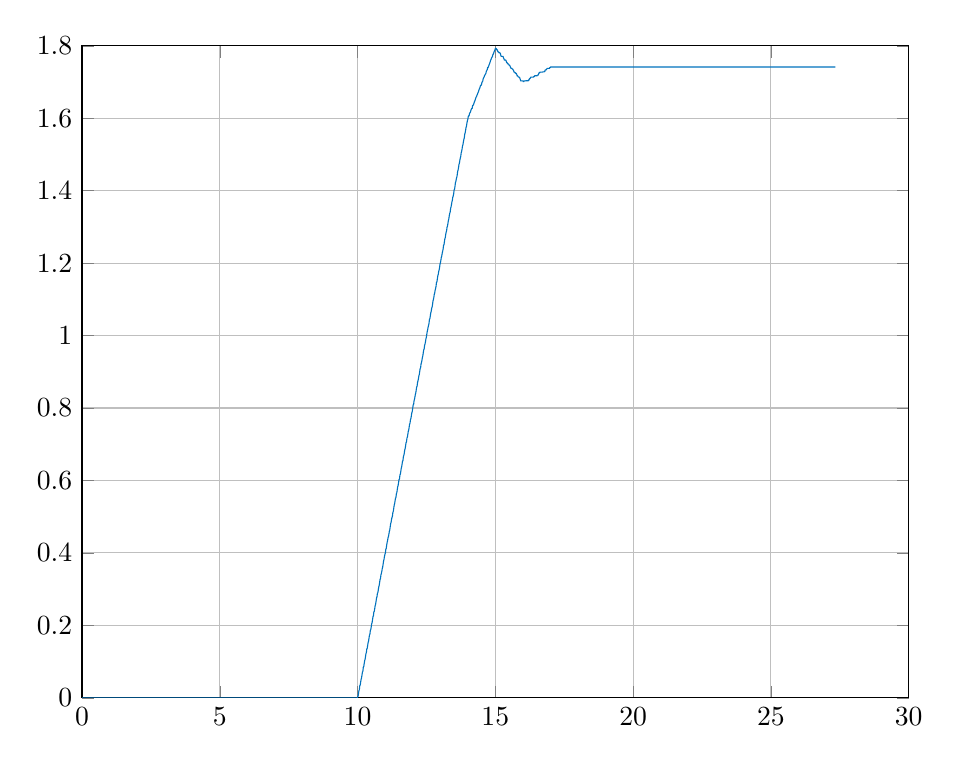
\begin{tikzpicture}

\begin{axis}[%
width=4.133in,
height=3.26in,
at={(0.693in,0.44in)},
scale only axis,
xmin=0,
xmax=30,
xmajorgrids,
ymin=0,
ymax=1.8,
ymajorgrids,
axis background/.style={fill=white}
]
\addplot [color=mycolor1,solid,forget plot]
  table[row sep=crcr]{%
0	0\\
0.017486686999999	0\\
0.0335484049999993	0\\
0.0489735169999991	0\\
0.0654204590000007	0\\
0.0807954470000006	0\\
0.095984534	0\\
0.111819789999999	0\\
0.127794892999999	0\\
0.143809515000999	0\\
0.159864158	0\\
0.176264448000001	0\\
0.191918061000001	0\\
0.208229863	0\\
0.22411426	0\\
0.240030810000001	0\\
0.255976952	0\\
0.271988863	0\\
0.288005780999999	0\\
0.303815257999999	0\\
0.319800566	0\\
0.335802525001001	0\\
0.351768663999999	0\\
0.36785526	0\\
0.383954799000001	0\\
0.399951771	0\\
0.415880339	0\\
0.431894845999999	0\\
0.447974014	0\\
0.463848232999999	0\\
0.480008339	0\\
0.495993414999001	0\\
0.511988127	0\\
0.528026147001	0\\
0.543979419999	0\\
0.560134905999999	0\\
0.576019073000001	0\\
0.591895217	0\\
0.607847277000001	0\\
0.623834802999999	0\\
0.639813487999	0\\
0.655864687999999	0\\
0.671844843	0\\
0.687894173	0\\
0.703960452998999	0\\
0.719861596999001	0\\
0.735862183	0\\
0.751862538000001	0\\
0.767889197000999	0\\
0.783981379999001	0\\
0.799994904999999	0\\
0.815962780998999	0\\
0.831992070999	0\\
0.847937220999999	0\\
0.863962322000001	0\\
0.879972584000001	0\\
0.896016072000001	0\\
0.912088118999999	0\\
0.927922307	0\\
0.944023716	0\\
0.959994168	0\\
0.975991230999	0\\
0.992029912	0\\
1.00793084	0\\
1.023850434	0\\
1.039763124	0\\
1.055901442	0\\
1.071836404	0\\
1.087869267	0\\
1.10386867	0\\
1.119916358	0\\
1.1358229	0\\
1.15185658	0\\
1.167908877	0\\
1.183846768001	0\\
1.199820039001	0\\
1.215989863	0\\
1.232047372	0\\
1.248097771	0\\
1.264938424	0\\
1.280224831001	0\\
1.295854792	0\\
1.311873158	0\\
1.327965721999	0\\
1.343997818	0\\
1.359990541	0\\
1.375953205	0\\
1.391990664	0\\
1.407983296	0\\
1.42398526	0\\
1.439988907	0\\
1.455918365999	0\\
1.471983127	0\\
1.487986744	0\\
1.50410443	0\\
1.519856507	0\\
1.536033372	0\\
1.551946803	0\\
1.568102883	0\\
1.583845648999	0\\
1.599816938	0\\
1.615792371001	0\\
1.631799331	0\\
1.647803028	0\\
1.663927058	0\\
1.680189577	0\\
1.695951467	0\\
1.711980451	0\\
1.727964409	0\\
1.744002825	0\\
1.760010982999	0\\
1.775946896	0\\
1.79184524	0\\
1.807861806	0\\
1.823847002	0\\
1.839834533	0\\
1.855985263	0\\
1.872113578	0\\
1.887788602	0\\
1.904080431	0\\
1.919815951	0\\
1.936070287999	0\\
1.95185823	0\\
1.967838134	0\\
1.983960635	0\\
2.000025140001	0\\
2.017650045	0\\
2.033143887	0\\
2.048642751	0\\
2.064027737	0\\
2.079982323	0\\
2.096419011999	0\\
2.11211212	0\\
2.127943664	0\\
2.144116339	0\\
2.1600051	0\\
2.175997858	0\\
2.191989798	0\\
2.207913897	0\\
2.22381201	0\\
2.239988593001	0\\
2.25599238	0\\
2.272004612	0\\
2.287857763001	0\\
2.303951063999	0\\
2.319942919	0\\
2.335980313	0\\
2.352239169	0\\
2.368013311	0\\
2.38401129	0\\
2.400130168	0\\
2.415943846	0\\
2.431985569	0\\
2.448257389	0\\
2.463981428001	0\\
2.479988824	0\\
2.495996796	0\\
2.512120174	0\\
2.528009412	0\\
2.543985026	0\\
2.560078320999	0\\
2.575957309	0\\
2.592038575	0\\
2.608019255	0\\
2.623982851	0\\
2.639868857001	0\\
2.655847989001	0\\
2.672064518	0\\
2.687855789	0\\
2.703825219	0\\
2.719867364	0\\
2.735848425	0\\
2.751841428	0\\
2.767796685999	0\\
2.783994127	0\\
2.799976426	0\\
2.815987054	0\\
2.831971804	0\\
2.847952003	0\\
2.864066180001	0\\
2.880101629999	0\\
2.896000037999	0\\
2.9119947	0\\
2.928207542	0\\
2.943964816	0\\
2.959980711001	0\\
2.975975097	0\\
2.991968672	0\\
3.008049589	0\\
3.025705628001	0\\
3.041302558	0\\
3.056294674	0\\
3.071707325	0\\
3.087762018	0\\
3.10588222	0\\
3.120848061	0\\
3.136017734	0\\
3.151834834	0\\
3.168017411001	0\\
3.183817157	0\\
3.199883506	0\\
3.215999618	0\\
3.231906530999	0\\
3.247868268	0\\
3.263899598999	0\\
3.279850943	0\\
3.295889188	0\\
3.311824488	0\\
3.330103953	0\\
3.34520471	0\\
3.360502328	0\\
3.376507724	0\\
3.391998727	0\\
3.407956905	0\\
3.423716052	0\\
3.439988605	0\\
3.455983166001	0\\
3.471984804	0\\
3.487860982001	0\\
3.506367524	0\\
3.521821832	0\\
3.536967627	0\\
3.552019848001	0\\
3.567876423001	0\\
3.583855765	0\\
3.600034659001	0\\
3.616012623	0\\
3.631974646	0\\
3.64803659	0\\
3.664004502	0\\
3.679872690999	0\\
3.696085323	0\\
3.712132148	0\\
3.728065185	0\\
3.743841969	0\\
3.759840189	0\\
3.775891353999	0\\
3.791852299	0\\
3.807891971	0\\
3.823991789999	0\\
3.840109428	0\\
3.855996638001	0\\
3.871925701	0\\
3.888081237001	0\\
3.903997015001	0\\
3.919870763	0\\
3.936023091999	0\\
3.951959091	0\\
3.967990361	0\\
3.983966682	0\\
3.99996206	0\\
4.017571706	0\\
4.032651770999	0\\
4.04783499	0\\
4.063893371001	0\\
4.079849379999	0\\
4.095843952001	0\\
4.111851974	0\\
4.127999232	0\\
4.14394607	0\\
4.159921162999	0\\
4.175822202999	0\\
4.191831913	0\\
4.20800091	0\\
4.223868114001	0\\
4.239983184	0\\
4.255981995	0\\
4.271850145001	0\\
4.287870174	0\\
4.303882005	0\\
4.320301229	0\\
4.335876135	0\\
4.351866602	0\\
4.367842502	0\\
4.383905609	0\\
4.399886439	0\\
4.415890207	0\\
4.431889204	0\\
4.44789114	0\\
4.463877956	0\\
4.48001681	0\\
4.495913405	0\\
4.511827202	0\\
4.527941767	0\\
4.543860352	0\\
4.559996389	0\\
4.576008185	0\\
4.591897362	0\\
4.607927595001	0\\
4.623936198	0\\
4.639968085	0\\
4.656080012	0\\
4.671823111	0\\
4.687780598	0\\
4.703962403	0\\
4.720163187	0\\
4.735872136999	0\\
4.751936527001	0\\
4.767989435	0\\
4.783966221999	0\\
4.799856497	0\\
4.815839142	0\\
4.831855848999	0\\
4.847988704	0\\
4.864022178999	0\\
4.879995537	0\\
4.895993602	0\\
4.912126157	0\\
4.928008574	0\\
4.944112568	0\\
4.959862902	0\\
4.976050516	0\\
4.992229881999	0\\
5.00798456	0\\
5.025727621	0\\
5.040911994	0\\
5.056201608	0\\
5.072061125	0\\
5.08785427	0\\
5.103860728	0\\
5.119839359	0\\
5.135849677	0\\
5.15183426	0\\
5.167928034	0\\
5.18420363	0\\
5.200012105	0\\
5.215974444	0\\
5.232035055001	0\\
5.247871685	0\\
5.263861435001	0\\
5.279974855999	0\\
5.295995893	0\\
5.312029757	0\\
5.32800208	0\\
5.343979879	0\\
5.359990474	0\\
5.377331107001	0\\
5.392508933	0\\
5.408060076	0\\
5.42388316	0\\
5.439875421	0\\
5.455980373	0\\
5.471983484	0\\
5.487966665	0\\
5.503868211001	0\\
5.51998506	0\\
5.535943665	0\\
5.551901649	0\\
5.567849605	0\\
5.583842257	0\\
5.5998659	0\\
5.615849357	0\\
5.63186656	0\\
5.647841391	0\\
5.663848662	0\\
5.679842938	0\\
5.695846786	0\\
5.711855354	0\\
5.727846343	0\\
5.74384761	0\\
5.759851372	0\\
5.775873983	0\\
5.791840385	0\\
5.807841377	0\\
5.823852486	0\\
5.839893136999	0\\
5.855842155	0\\
5.871846494	0\\
5.887839251999	0\\
5.903850416001	0\\
5.919859576	0\\
5.935856994	0\\
5.951836722	0\\
5.967980768	0\\
5.98396902	0\\
5.999988959	0\\
6.017461794	0\\
6.032542141	0\\
6.047851054	0\\
6.063789746	0\\
6.079982419	0\\
6.096028804	0\\
6.112197169	0\\
6.127987843999	0\\
6.14400659	0\\
6.160620305	0\\
6.175926587	0\\
6.191874924	0\\
6.207853971	0\\
6.223858966	0\\
6.239991129	0\\
6.255961035	0\\
6.271965805	0\\
6.287855514	0\\
6.303849871	0\\
6.319843220001	0\\
6.335992677	0\\
6.352068348	0\\
6.367996268999	0\\
6.383986896	0\\
6.399983683	0\\
6.415981171	0\\
6.432326658	0\\
6.448015282	0\\
6.463933515	0\\
6.479989165	0\\
6.495996857	0\\
6.511966723	0\\
6.527969363	0\\
6.543976087	0\\
6.560117987001	0\\
6.576019849	0\\
6.591898213001	0\\
6.60800549	0\\
6.623987182	0\\
6.639978992999	0\\
6.655979738	0\\
6.671970694	0\\
6.687890725	0\\
6.703959956	0\\
6.719903061	0\\
6.736118653	0\\
6.751990346	0\\
6.767856928	0\\
6.783841984	0\\
6.800109087	0\\
6.815839205	0\\
6.83184929	0\\
6.84785296	0\\
6.863820206	0\\
6.879848282	0\\
6.896027948	0\\
6.912100356	0\\
6.927857114	0\\
6.94401239	0\\
6.960079546	0\\
6.975990438	0\\
6.991984544	0\\
7.007979692001	0\\
7.023862178001	0\\
7.039860893001	0\\
7.055952778	0\\
7.07198731	0\\
7.08787378	0\\
7.104000367999	0\\
7.119878782	0\\
7.135843636	0\\
7.151983467	0\\
7.167992752	0\\
7.183983109	0\\
7.199993135	0\\
7.215927987	0\\
7.231990959	0\\
7.248110008	0\\
7.263994520001	0\\
7.279978317	0\\
7.29598012	0\\
7.311967852	0\\
7.327984884	0\\
7.344036841	0\\
7.359991648	0\\
7.375941638001	0\\
7.391957109	0\\
7.407991825	0\\
7.423983791001	0\\
7.440299411001	0\\
7.455997626001	0\\
7.472022897001	0\\
7.487877721	0\\
7.503976749999	0\\
7.519847844	0\\
7.535793886999	0\\
7.551727271	0\\
7.567746317	0\\
7.583805196	0\\
7.599885973	0\\
7.616033161001	0\\
7.631984665	0\\
7.648047667	0\\
7.66399407	0\\
7.679875387	0\\
7.695933044	0\\
7.711983202	0\\
7.727866161001	0\\
7.743846445	0\\
7.759983444001	0\\
7.776080985	0\\
7.792035334999	0\\
7.808116768	0\\
7.824087381	0\\
7.839867387	0\\
7.855851194	0\\
7.871966544	0\\
7.887853167	0\\
7.904021978	0\\
7.919860643001	0\\
7.935857589	0\\
7.951844027	0\\
7.967842142	0\\
7.983788231	0\\
7.999854768999	0\\
8.017226094	0\\
8.03242936	0\\
8.048033415	0\\
8.064008172	0\\
8.079984532999	0\\
8.096111955	0\\
8.111885089999	0\\
8.127851588	0\\
8.143970061	0\\
8.159966487	0\\
8.175972364001	0\\
8.191934654001	0\\
8.207990388	0\\
8.22399195	0\\
8.239967028	0\\
8.255991984	0\\
8.271880347	0\\
8.288003969	0\\
8.303895738	0\\
8.319890578	0\\
8.335951235999	0\\
8.351928202999	0\\
8.367844089	0\\
8.383987025	0\\
8.400064459	0\\
8.415987574001	0\\
8.431715610999	0\\
8.447955805001	0\\
8.46409959	0\\
8.479920212	0\\
8.49595922	0\\
8.511975155	0\\
8.527807334	0\\
8.543956756	0\\
8.559932374999	0\\
8.575968185	0\\
8.591881277	0\\
8.607929852	0\\
8.623839445	0\\
8.639833406	0\\
8.65585092	0\\
8.671917865	0\\
8.687842158	0\\
8.704015207	0\\
8.719831747	0\\
8.73599239	0\\
8.752517784001	0\\
8.768091072	0\\
8.784067327	0\\
8.800030593001	0\\
8.815993513	0\\
8.832163016	0\\
8.847965497	0\\
8.863975243	0\\
8.879895853	0\\
8.896028878001	0\\
8.911957110001	0\\
8.927983173	0\\
8.943893871001	0\\
8.959987576	0\\
8.975998971	0\\
8.992018459	0\\
9.007844945	0\\
9.025491622	0\\
9.040655504	0\\
9.05585089	0\\
9.071831285	0\\
9.087846854	0\\
9.103835227	0\\
9.119997669	0\\
9.13599966	0\\
9.151983379999	0\\
9.167836060001	0\\
9.183965129	0\\
9.199993144	0\\
9.21585087	0\\
9.231846695	0\\
9.24799586	0\\
9.263971531	0\\
9.27998909	0\\
9.296005692	0\\
9.312029775	0\\
9.327963308	0\\
9.343974773	0\\
9.359985577	0\\
9.376000405	0\\
9.392563669	0\\
9.407995697001	0\\
9.423989913	0\\
9.44008832	0\\
9.455951188	0\\
9.471966218	0\\
9.48797065	0\\
9.503844253	0\\
9.520148461	0\\
9.536045297	0\\
9.553297377	0\\
9.568767485	0\\
9.584163717	0\\
9.600208683	0\\
9.615995278	0\\
9.632013268	0\\
9.647977641	0\\
9.663963448	0\\
9.680035245	0\\
9.696007496001	0\\
9.711999838	0\\
9.727993923	0\\
9.744061065	0\\
9.760017875	0\\
9.776223054	0\\
9.792048017	0\\
9.807948174999	0\\
9.823957148999	0\\
9.839880228999	0\\
9.855805168	0\\
9.871788309	0\\
9.887849892	0\\
9.903951436	0\\
9.919780925	0\\
9.935843455	0\\
9.952036546	0\\
9.967985144	0\\
9.9840059	0\\
10.000018628	0.00195929075870865\\
10.017668344	0.00391858151741729\\
10.033358506	0.0117561525575638\\
10.048801532999	0.0199947667571325\\
10.063992134	0.0219543385127193\\
10.079961859	0.0333555692763681\\
10.096000586	0.0353148493261139\\
10.111954488	0.0431523983171564\\
10.127834398	0.0509889104837971\\
10.144004251	0.0549077008684895\\
10.159905171001	0.0627445374472635\\
10.175990233	0.0709833458951193\\
10.191972571	0.0729431078622516\\
10.207959466001	0.0843467322174817\\
10.223868092	0.0863057422184539\\
10.239857909	0.0941423127639337\\
10.255848978	0.10197826851671\\
10.271971805	0.105896708879398\\
10.287994816	0.113732857130316\\
10.303905493	0.121971725332057\\
10.319956954	0.124743095597818\\
10.335998406	0.135337214025708\\
10.351968337	0.137296220021645\\
10.367869703	0.145132204864222\\
10.383860541	0.152967286969737\\
10.399866719	0.156885334579459\\
10.415861216001	0.1651249272999\\
10.432036196	0.172959927045449\\
10.448021021	0.175732916424795\\
10.463938207	0.186327829330511\\
10.480249577001	0.188286487041644\\
10.496029262	0.196121625028826\\
10.511966554	0.203956073442876\\
10.528000834999	0.20787381101624\\
10.543984898	0.216113757068755\\
10.559988415	0.223947353347441\\
10.576110942	0.227122129784937\\
10.592011831	0.237317773852279\\
10.60798081	0.239276454543243\\
10.623987157999	0.247110894177621\\
10.639983234	0.254944534042368\\
10.655962586001	0.258861772823795\\
10.672021563	0.267101655856662\\
10.68785515	0.275344544675247\\
10.703839729	0.278515199458051\\
10.72001495	0.288307715708748\\
10.736290253	0.290265942274672\\
10.752002325	0.29809968841717\\
10.767928587	0.305932623145191\\
10.78396365	0.310256375473006\\
10.800014529001	0.318089693365345\\
10.815968128	0.326740924049042\\
10.831995911	0.329505673476397\\
10.847990132	0.339297015771402\\
10.864021076	0.343214463666393\\
10.879858917	0.349088233274227\\
10.895994147	0.356920418719696\\
10.912003758999	0.361244351780684\\
10.927812883	0.369076987908514\\
10.944089962	0.377729461849186\\
10.960012951	0.382453552557871\\
10.975967372	0.390286158368493\\
10.994437291	0.396160593342135\\
11.009855928	0.400076210326825\\
11.024862852	0.409866130263916\\
11.040363161001	0.412232397446914\\
11.055893209	0.420886334013296\\
11.071954883	0.428717367482197\\
11.08799588	0.433442924041582\\
11.103866797	0.441274687125049\\
11.119979726	0.445191290153753\\
11.135979645	0.451063850761079\\
11.152036092	0.459304041808284\\
11.167860453	0.463219477822907\\
11.183752573	0.471874482418661\\
11.199759137	0.480515918703082\\
11.215828492999	0.484431997085672\\
11.231808772	0.492262924328079\\
11.250404881999	0.498136247567149\\
11.265866270999	0.502050996717277\\
11.281521764	0.512249133016502\\
11.296757813	0.514620121737281\\
11.311903121001	0.522862654758944\\
11.327865785	0.531504900838892\\
11.343986763	0.53542025825273\\
11.359975071	0.543250541444703\\
11.376366240999	0.551079980237494\\
11.392050157	0.55303774263945\\
11.407961721	0.563235939216815\\
11.423941196	0.566019954824606\\
11.439990165	0.574255662832523\\
11.455954879	0.58249311096244\\
11.472048105001	0.586408283996973\\
11.487916396	0.594237780608164\\
11.503695352	0.602066494085029\\
11.521699371	0.604435499526949\\
11.536536236	0.61463701158548\\
11.551689432	0.617007589834535\\
11.569768705	0.625652643373812\\
11.584946473001	0.633480992617072\\
11.600190114001	0.637395581577943\\
11.615752999999	0.645224260733243\\
11.631693449999	0.653052227569402\\
11.647688898999	0.655422329080311\\
11.663683103	0.66603799155969\\
11.681889187001	0.669951134804266\\
11.697101984	0.676640493015479\\
11.712128372	0.684468105720095\\
11.727860143	0.68838243421456\\
11.743847957	0.696210298865991\\
11.759921565999	0.704450906627083\\
11.775981921	0.706824694144621\\
11.791976771	0.717024405863653\\
11.80795432	0.71939183583523\\
11.824044034	0.727627941846543\\
11.839996891	0.735454849726604\\
11.856056169	0.739368661040702\\
11.872050741	0.747195575372764\\
11.888032609	0.755436310298784\\
11.903815577	0.758226938647369\\
11.919827874	0.76801046731857\\
11.935811235	0.770787880660686\\
11.951821115999	0.778614678622068\\
11.967815132	0.786440647074948\\
11.983844497	0.790354214763538\\
11.99986148	0.79859571457446\\
12.017454397001	0.808796517979441\\
12.032719391	0.809213181143731\\
12.048030129	0.818995883055397\\
12.06400678	0.823732152751271\\
12.079982388999	0.829600778637035\\
12.095891701	0.837426022504511\\
12.111777777	0.841339068505069\\
12.127842794999	0.849580300358285\\
12.143991495	0.858242238273216\\
12.160025336	0.860199086538433\\
12.175987049	0.87039374789121\\
12.191947357	0.874718317910754\\
12.208013426	0.880586295378968\\
12.223962285	0.888410513161725\\
12.239861184	0.892739898904362\\
12.255963174999	0.900985001869094\\
12.27186019	0.90922743287563\\
12.287836821	0.911183879597191\\
12.303870627	0.921790539770876\\
12.319859446	0.925703493882202\\
12.33582852	0.931570920773396\\
12.351935486	0.939394639881869\\
12.36785407	0.94372441434851\\
12.383869876	0.95238834902311\\
12.399881065	0.960211966540132\\
12.415860973	0.962583194177171\\
12.431885087	0.972775496015762\\
12.447991928	0.976688050433576\\
12.463975985999	0.982555110315896\\
12.479967546001	0.99079579464459\\
12.49600742	0.995129574096111\\
12.512026683001	1.0033731473321\\
12.527979592	1.01119540181499\\
12.543979208	1.01593666610025\\
12.560080973	1.02375987567632\\
12.575893131	1.02767185286547\\
12.591957772001	1.03353813528736\\
12.607991342	1.04415808559281\\
12.623822784	1.0465342561868\\
12.639977123	1.05435665561113\\
12.655959401	1.06259523995848\\
12.671949513	1.06692083028304\\
12.687982597	1.07474318099976\\
12.704035315	1.07865492888785\\
12.720021768	1.08494048708576\\
12.736016075	1.0951408403407\\
12.751875165	1.09947425657462\\
12.767797132	1.10533986157871\\
12.783836501	1.11399313974728\\
12.800182779	1.11790441802295\\
12.816031766	1.12572608329139\\
12.831965990999	1.12963688876271\\
12.848031032	1.13634680570089\\
12.86399961	1.14654594711762\\
12.879938294999	1.14850037977558\\
12.895996756	1.15673996783221\\
12.912105462	1.16497631775798\\
12.92792629	1.16888674531932\\
12.943839041	1.17670761189332\\
12.959855833	1.18104017004783\\
12.976032022	1.18775260359598\\
12.99201621	1.19752792354879\\
13.007858497	1.20143889619749\\
13.023792321	1.20813870598505\\
13.039744899	1.21595827518656\\
13.05591623	1.21986843599691\\
13.071846596	1.22768854379039\\
13.087981905999	1.23244668271075\\
13.103950594	1.23873489193153\\
13.120117336	1.24850979820642\\
13.136024737	1.25088342808191\\
13.151997252	1.25912086345168\\
13.167858489	1.26693982625676\\
13.183939222	1.27084894548704\\
13.199923226	1.27951794832506\\
13.215962118	1.28580748131857\\
13.231953358	1.28971616535515\\
13.248001446	1.29948984680208\\
13.263987298001	1.30228302234755\\
13.279980055	1.31010171794896\\
13.296214871	1.31791983156148\\
13.312134383001	1.32225317590597\\
13.328006872999	1.33092451266319\\
13.343871655999	1.33678812268356\\
13.359846959	1.34069682125624\\
13.376176419	1.35089098968993\\
13.391998771	1.35521939906714\\
13.407951793	1.36108188419315\\
13.423934056999	1.3688996485314\\
13.440016056999	1.37366044974873\\
13.455928718001	1.38190498470828\\
13.47200945	1.3858145989605\\
13.487994726	1.39167585216295\\
13.503930695	1.40229023125838\\
13.520122669	1.40424412112732\\
13.535994387	1.41206062732352\\
13.552143063	1.42268657512834\\
13.567978359	1.42506765853592\\
13.583843648	1.43288473642861\\
13.599871936	1.43679336151409\\
13.615848983	1.44307799965186\\
13.632066635	1.4532691577886\\
13.648000169	1.4571780055111\\
13.663961109	1.46346567366241\\
13.679905552	1.47213896032879\\
13.695858747999	1.47604672062931\\
13.711932391	1.48386307291891\\
13.72796795	1.49014914492234\\
13.743951187001	1.49447750474113\\
13.759979856	1.50424734389641\\
13.776030564	1.50815626451194\\
13.7920226	1.51487339177463\\
13.807942248	1.52311764132488\\
13.823999681999	1.52702562351866\\
13.84001694	1.53483997816272\\
13.856214341001	1.54112679285349\\
13.872008414	1.54545610178194\\
13.887983235	1.55522421597514\\
13.903994861	1.55999141744094\\
13.919937625	1.56628126593932\\
13.936033271	1.57409541188004\\
13.951986549	1.57800240876508\\
13.967998911001	1.58624253966634\\
13.983962302	1.59252669656045\\
13.999994825	1.59643270317195\\
14.017505371001	1.60467942250916\\
14.032585284999	1.60663299166837\\
14.047964185	1.60663299166837\\
14.063867397001	1.6133536361109\\
14.080146228	1.61530645451251\\
14.095993591	1.61726002367171\\
14.111979188	1.6211688732894\\
14.127994191	1.62507488621513\\
14.143957306	1.62745417508715\\
14.159874658	1.62745417508715\\
14.175938191	1.63526903763057\\
14.191981277	1.63569236956274\\
14.207869819001	1.63764593872194\\
14.223915171	1.64155478833963\\
14.239848654	1.64546080126536\\
14.255865086	1.64741437042457\\
14.271942861	1.65175507683604\\
14.288025542	1.65566108976178\\
14.303891578	1.65847325922171\\
14.319946526	1.66042742470245\\
14.336028761	1.66433530336352\\
14.351872246	1.66628812176512\\
14.367987801999	1.67062157611789\\
14.384143343001	1.67257626025483\\
14.399955962	1.67648227318056\\
14.415984035	1.68039000782051\\
14.431957684	1.68234469195745\\
14.448025066	1.68667403681535\\
14.463973187	1.6905817714553\\
14.480037472	1.6905817714553\\
14.495865577	1.69253645559224\\
14.512023894	1.69882849079251\\
14.527988935	1.70078205995172\\
14.544015689	1.70273674408866\\
14.559991834	1.70945552279586\\
14.575987177	1.71140909195507\\
14.591970228	1.71378949580482\\
14.607939893999	1.71769685580969\\
14.623969289	1.7196496742113\\
14.640000322999	1.72160324337051\\
14.656042072	1.72355792750745\\
14.671992744001	1.72941810591392\\
14.68785877	1.7317950070053\\
14.703814629	1.73374969114224\\
14.719799759	1.73960986954871\\
14.735826303	1.73960986954871\\
14.751810757	1.74351812284486\\
14.767883837	1.74590414511939\\
14.784403879	1.74981015804513\\
14.799988823	1.75262232750506\\
14.815851666	1.75653117712274\\
14.831857779	1.76086290976129\\
14.847833027001	1.7628164789205\\
14.863882498	1.76672532853818\\
14.879853897	1.76867852306231\\
14.895881478	1.77063134146392\\
14.911957279	1.7764937602408\\
14.928018539	1.77691709217297\\
14.944133376	1.78082310509871\\
14.959996134	1.78473083973865\\
14.97601438	1.78668552387559\\
14.991969301999	1.79059153680133\\
15.007964845	1.79297755907586\\
15.025661518	1.79297755907586\\
15.040820341	1.79102293039607\\
15.056224806	1.78863750444307\\
15.071796811	1.78863750444307\\
15.08784769	1.78473149151733\\
15.103984965	1.78277633322473\\
15.120584066	1.78277633322473\\
15.136154065999	1.78082231646726\\
15.15209219	1.78082190580592\\
15.167991652	1.78039857387375\\
15.183706164001	1.77844500471454\\
15.201759735	1.77258388609347\\
15.217388007	1.77063001829735\\
15.232905603	1.77063001829735\\
15.248296016	1.77062966041186\\
15.263963767	1.77062966041186\\
15.280054823	1.77062966041186\\
15.296020414001	1.7667210383927\\
15.311987974	1.76476731979601\\
15.328046937	1.76086130687028\\
15.343970919	1.76086100199875\\
15.359881395	1.76086100199875\\
15.375884486	1.76043289514072\\
15.391968254	1.75847925123302\\
15.407997786	1.7541419682405\\
15.424042336	1.7541419682405\\
15.439856964999	1.75023595531477\\
15.456127652001	1.75023536273967\\
15.471978052	1.75023536273967\\
15.487966064	1.74828186838847\\
15.503843471	1.74632665583855\\
15.519966161	1.74589650336452\\
15.535982535	1.74394293420531\\
15.551979686	1.74003638222073\\
15.568175523999	1.73808303766406\\
15.583861907	1.73808303766406\\
15.599826639	1.73765070615208\\
15.615854448	1.73569602201514\\
15.631846093	1.73569602201514\\
15.647848268	1.73331863561924\\
15.663838434	1.73136544109511\\
15.679902148	1.72745942816937\\
15.696025843001	1.72745942816937\\
15.711890284	1.7255043232471\\
15.727964952	1.7255043232471\\
15.743914416001	1.72355120382849\\
15.760064105	1.72355084768136\\
15.775993890001	1.72116644428083\\
15.791955356	1.71726043135509\\
15.80799266	1.71725972387669\\
15.823964861	1.71530503973975\\
15.839869749	1.71335207071066\\
15.855842507	1.71335142806209\\
15.871849867999	1.71335142806209\\
15.88790435	1.71139785890288\\
15.904392189	1.70749119293392\\
15.919982515001	1.70358369039537\\
15.935988683	1.70315524256868\\
15.951957441	1.7031546545338\\
15.967857509	1.7031546545338\\
15.983846212	1.7031546545338\\
15.999962339	1.70315405616378\\
16.017517646	1.70120138862761\\
16.032688442	1.70120138862761\\
16.048149896	1.70315405616378\\
16.064113332999	1.70315405616378\\
16.080008785	1.70315405616378\\
16.095961627	1.70315405616378\\
16.112004764	1.70358250399048\\
16.127964431999	1.70358250399048\\
16.143976628	1.70358250399048\\
16.160000321	1.70358250399048\\
16.17607249	1.70358250399048\\
16.191987274	1.70358250399048\\
16.208037217	1.70553718812742\\
16.22399262	1.70553718812742\\
16.239877232	1.7094434248228\\
16.255945610999	1.7094434248228\\
16.271848865999	1.71139661934693\\
16.28784699	1.71334943774853\\
16.303847586	1.71334943774853\\
16.319818905	1.71334943774853\\
16.335847704	1.71334943774853\\
16.352030929	1.71334943774853\\
16.367970390001	1.71334943774853\\
16.383715136	1.71334943774853\\
16.399728560001	1.71530412188548\\
16.415784848001	1.71530412188548\\
16.431910035	1.71725678942165\\
16.447990225	1.71725678942165\\
16.463950805	1.71725678942165\\
16.479734909	1.71725678942165\\
16.495704999	1.71725678942165\\
16.513856678	1.71725678942165\\
16.52875146	1.71921035858086\\
16.543922847	1.71921035858086\\
16.560009081	1.71964289701055\\
16.576072243	1.72354890993628\\
16.59196082	1.72550359407322\\
16.607864129999	1.72550359407322\\
16.623845196	1.7274562616094\\
16.639820183999	1.7274562616094\\
16.655829082	1.7274562616094\\
16.671829252	1.7274562616094\\
16.687915456	1.7274562616094\\
16.703969924	1.7274562616094\\
16.719966269	1.72787959354157\\
16.735964615	1.72787959354157\\
16.751957543	1.72787959354157\\
16.767959055001	1.72787959354157\\
16.783785306	1.72983427767851\\
16.799734558999	1.72983427767851\\
16.815733957	1.73374051437389\\
16.833800629	1.73374051437389\\
16.848679415	1.73374051437389\\
16.863706291	1.73569370889802\\
16.881760272	1.73764652729963\\
16.896666697001	1.73764652729963\\
16.911775562001	1.73764652729963\\
16.927722907	1.73764652729963\\
16.943940587	1.73764652729963\\
16.959902704	1.73764652729963\\
16.975753610999	1.73960121143657\\
16.9921274	1.73960121143657\\
17.008000469	1.74155387897275\\
17.025863544	1.74155387897275\\
17.041092426	1.74155387897275\\
17.056177337	1.74155387897275\\
17.071869559	1.74155387897275\\
17.087918299	1.74155387897275\\
17.104006935	1.74155387897275\\
17.119897072999	1.74155387897275\\
17.135990688999	1.74155387897275\\
17.152013084	1.74155387897275\\
17.167959011	1.74155387897275\\
17.183838131001	1.74155387897275\\
17.199848980001	1.74155387897275\\
17.21596468	1.74155387897275\\
17.232027246	1.74155387897275\\
17.248034041	1.74155387897275\\
17.26396996	1.74155387897275\\
17.279975657	1.74155387897275\\
17.295859492	1.74155387897275\\
17.311968058	1.74155387897275\\
17.327984694	1.74155387897275\\
17.343860296	1.74155387897275\\
17.359852703	1.74155387897275\\
17.376004651	1.74155387897275\\
17.391890747	1.74155387897275\\
17.407816312	1.74155387897275\\
17.42391026	1.74155387897275\\
17.439815258001	1.74155387897275\\
17.455978096	1.74155387897275\\
17.471736298001	1.74155387897275\\
17.489935733	1.74155387897275\\
17.504925426	1.74155387897275\\
17.520689742	1.74155387897275\\
17.537219983	1.74155387897275\\
17.552052568	1.74155387897275\\
17.567695725001	1.74155387897275\\
17.585743891	1.74155387897275\\
17.600662918	1.74155387897275\\
17.616058233	1.74155387897275\\
17.631712181	1.74155387897275\\
17.649805993	1.74155387897275\\
17.6647244	1.74155387897275\\
17.679697486	1.74155387897275\\
17.697803862001	1.74155387897275\\
17.712675811	1.74155387897275\\
17.727703604	1.74155387897275\\
17.745704318	1.74155387897275\\
17.760588605	1.74155387897275\\
17.77569267	1.74155387897275\\
17.793704681	1.74155387897275\\
17.808644798	1.74155387897275\\
17.823708869	1.74155387897275\\
17.841774325	1.74155387897275\\
17.856663253	1.74155387897275\\
17.871696656	1.74155387897275\\
17.889769353	1.74155387897275\\
17.904684919	1.74155387897275\\
17.919760850001	1.74155387897275\\
17.937756297	1.74155387897275\\
17.952573419	1.74155387897275\\
17.967702661001	1.74155387897275\\
17.985722971999	1.74155387897275\\
18.00056186	1.74155387897275\\
18.017619308	1.74155387897275\\
18.03246994	1.74155387897275\\
18.047725777001	1.74155387897275\\
18.063774362001	1.74155387897275\\
18.081891108	1.74155387897275\\
18.097230375	1.74155387897275\\
18.112469846999	1.74155387897275\\
18.127907624	1.74155387897275\\
18.143765162	1.74155387897275\\
18.159796461	1.74155387897275\\
18.175803470001	1.74155387897275\\
18.193939686	1.74155387897275\\
18.207885768	1.74155387897275\\
18.223738921	1.74155387897275\\
18.239895754	1.74155387897275\\
18.255822669999	1.74155387897275\\
18.272403217	1.74155387897275\\
18.287829009	1.74155387897275\\
18.30393959	1.74155387897275\\
18.319756306	1.74155387897275\\
18.337959949001	1.74155387897275\\
18.352987810001	1.74155387897275\\
18.367927133	1.74155387897275\\
18.38382451	1.74155387897275\\
18.399720395	1.74155387897275\\
18.417809681	1.74155387897275\\
18.432670225	1.74155387897275\\
18.447838515	1.74155387897275\\
18.463791142	1.74155387897275\\
18.479975811	1.74155387897275\\
18.495888361	1.74155387897275\\
18.511961516	1.74155387897275\\
18.527858214999	1.74155387897275\\
18.543979428	1.74155387897275\\
18.559893312001	1.74155387897275\\
18.575853355999	1.74155387897275\\
18.591852267	1.74155387897275\\
18.607859628	1.74155387897275\\
18.623843606	1.74155387897275\\
18.639897752	1.74155387897275\\
18.655996613	1.74155387897275\\
18.671965885	1.74155387897275\\
18.687963403	1.74155387897275\\
18.704104852	1.74155387897275\\
18.71988154	1.74155387897275\\
18.735844577999	1.74155387897275\\
18.751749129	1.74155387897275\\
18.767761343	1.74155387897275\\
18.783830404001	1.74155387897275\\
18.799738565	1.74155387897275\\
18.815954623	1.74155387897275\\
18.832014064	1.74155387897275\\
18.847959128	1.74155387897275\\
18.863999118	1.74155387897275\\
18.879987942	1.74155387897275\\
18.896069546	1.74155387897275\\
18.912179639	1.74155387897275\\
18.927993396	1.74155387897275\\
18.943971209999	1.74155387897275\\
18.959987376001	1.74155387897275\\
18.976096762	1.74155387897275\\
18.991990816	1.74155387897275\\
19.00837016	1.74155387897275\\
19.024136915	1.74155387897275\\
19.039973013	1.74155387897275\\
19.055886366	1.74155387897275\\
19.071963731	1.74155387897275\\
19.087959921	1.74155387897275\\
19.103970785	1.74155387897275\\
19.119880388	1.74155387897275\\
19.135965801	1.74155387897275\\
19.151980433	1.74155387897275\\
19.167970291999	1.74155387897275\\
19.184376558999	1.74155387897275\\
19.200135076	1.74155387897275\\
19.215870566	1.74155387897275\\
19.231859289	1.74155387897275\\
19.247869326	1.74155387897275\\
19.266232589999	1.74155387897275\\
19.281389287	1.74155387897275\\
19.296521419999	1.74155387897275\\
19.311771995	1.74155387897275\\
19.327852117	1.74155387897275\\
19.343865992	1.74155387897275\\
19.360196094	1.74155387897275\\
19.376004529	1.74155387897275\\
19.391718386	1.74155387897275\\
19.410013238	1.74155387897275\\
19.425320156	1.74155387897275\\
19.440931054	1.74155387897275\\
19.456409150999	1.74155387897275\\
19.471845428	1.74155387897275\\
19.487843553001	1.74155387897275\\
19.503830287	1.74155387897275\\
19.519884809	1.74155387897275\\
19.535986303001	1.74155387897275\\
19.551939708	1.74155387897275\\
19.567995567	1.74155387897275\\
19.583984243	1.74155387897275\\
19.599996352	1.74155387897275\\
19.616050418	1.74155387897275\\
19.631867929	1.74155387897275\\
19.647839914999	1.74155387897275\\
19.663872558	1.74155387897275\\
19.679829223	1.74155387897275\\
19.695911589	1.74155387897275\\
19.711940884	1.74155387897275\\
19.727959892	1.74155387897275\\
19.74401462	1.74155387897275\\
19.759989056	1.74155387897275\\
19.775777585	1.74155387897275\\
19.791667472	1.74155387897275\\
19.807666350999	1.74155387897275\\
19.823674697	1.74155387897275\\
19.839739436	1.74155387897275\\
19.855661152001	1.74155387897275\\
19.871681181	1.74155387897275\\
19.887671569	1.74155387897275\\
19.905883468001	1.74155387897275\\
19.921355597	1.74155387897275\\
19.936829629	1.74155387897275\\
19.952205680001	1.74155387897275\\
19.968050162	1.74155387897275\\
19.983996735	1.74155387897275\\
20.000027001999	1.74155387897275\\
20.017910129	1.74155387897275\\
20.033451207	1.74155387897275\\
20.04868516	1.74155387897275\\
20.064084938999	1.74155387897275\\
20.079990319001	1.74155387897275\\
20.095977964999	1.74155387897275\\
20.111995218	1.74155387897275\\
20.128131526	1.74155387897275\\
20.143989683999	1.74155387897275\\
20.159978207	1.74155387897275\\
20.175972017	1.74155387897275\\
20.19198494	1.74155387897275\\
20.207866581	1.74155387897275\\
20.223800746	1.74155387897275\\
20.239961283	1.74155387897275\\
20.255979454	1.74155387897275\\
20.273507522001	1.74155387897275\\
20.287962244	1.74155387897275\\
20.304000609	1.74155387897275\\
20.320096219	1.74155387897275\\
20.335855664	1.74155387897275\\
20.351874084001	1.74155387897275\\
20.367978149	1.74155387897275\\
20.383783703	1.74155387897275\\
20.401827682	1.74155387897275\\
20.416707212	1.74155387897275\\
20.431880138	1.74155387897275\\
20.447930686	1.74155387897275\\
20.463844295	1.74155387897275\\
20.479835183	1.74155387897275\\
20.495845706	1.74155387897275\\
20.511921096	1.74155387897275\\
20.527785999	1.74155387897275\\
20.543962663	1.74155387897275\\
20.559966256	1.74155387897275\\
20.57593645	1.74155387897275\\
20.591972908	1.74155387897275\\
20.60797373	1.74155387897275\\
20.624033890001	1.74155387897275\\
20.639914969	1.74155387897275\\
20.655931386	1.74155387897275\\
20.671876701	1.74155387897275\\
20.687855126	1.74155387897275\\
20.70385735	1.74155387897275\\
20.719855615	1.74155387897275\\
20.735844088001	1.74155387897275\\
20.751865796001	1.74155387897275\\
20.767877857001	1.74155387897275\\
20.783880227	1.74155387897275\\
20.799809681	1.74155387897275\\
20.815843176	1.74155387897275\\
20.831861903	1.74155387897275\\
20.847868502	1.74155387897275\\
20.863698093999	1.74155387897275\\
20.879664898	1.74155387897275\\
20.895660773999	1.74155387897275\\
20.913927903	1.74155387897275\\
20.928990644	1.74155387897275\\
20.944062575	1.74155387897275\\
20.959883113	1.74155387897275\\
20.97596645	1.74155387897275\\
20.991900109	1.74155387897275\\
21.007984704999	1.74155387897275\\
21.025902839	1.74155387897275\\
21.041257822	1.74155387897275\\
21.056469720001	1.74155387897275\\
21.07183648	1.74155387897275\\
21.087887495	1.74155387897275\\
21.103923209999	1.74155387897275\\
21.119849066	1.74155387897275\\
21.135845562	1.74155387897275\\
21.151873369001	1.74155387897275\\
21.167882845	1.74155387897275\\
21.183990051	1.74155387897275\\
21.199931513	1.74155387897275\\
21.215854532	1.74155387897275\\
21.231965543	1.74155387897275\\
21.247999834	1.74155387897275\\
21.263992527	1.74155387897275\\
21.280046296	1.74155387897275\\
21.295954388999	1.74155387897275\\
21.31197509	1.74155387897275\\
21.327860519	1.74155387897275\\
21.343964478	1.74155387897275\\
21.359964341999	1.74155387897275\\
21.375853001001	1.74155387897275\\
21.391722498	1.74155387897275\\
21.409801405999	1.74155387897275\\
21.424854324	1.74155387897275\\
21.440132298	1.74155387897275\\
21.457224084999	1.74155387897275\\
21.47238687	1.74155387897275\\
21.487794565999	1.74155387897275\\
21.50639076	1.74155387897275\\
21.520904986	1.74155387897275\\
21.537640012	1.74155387897275\\
21.553210533	1.74155387897275\\
21.568698989	1.74155387897275\\
21.584111617	1.74155387897275\\
21.599913658	1.74155387897275\\
21.615960864	1.74155387897275\\
21.631866133	1.74155387897275\\
21.64799785	1.74155387897275\\
21.66396042	1.74155387897275\\
21.679854032999	1.74155387897275\\
21.695834422	1.74155387897275\\
21.711839172	1.74155387897275\\
21.727991546	1.74155387897275\\
21.743981202	1.74155387897275\\
21.760266533	1.74155387897275\\
21.775728627	1.74155387897275\\
21.79166907	1.74155387897275\\
21.807703426	1.74155387897275\\
21.82365321	1.74155387897275\\
21.839691584	1.74155387897275\\
21.855711001	1.74155387897275\\
21.871678298001	1.74155387897275\\
21.887871279	1.74155387897275\\
21.903849634	1.74155387897275\\
21.919842863	1.74155387897275\\
21.935853396	1.74155387897275\\
21.95184474	1.74155387897275\\
21.967850421999	1.74155387897275\\
21.983850281	1.74155387897275\\
21.999823795	1.74155387897275\\
22.017495987	1.74155387897275\\
22.03191975	1.74155387897275\\
22.047981485	1.74155387897275\\
22.063968441	1.74155387897275\\
22.080108298001	1.74155387897275\\
22.095915235999	1.74155387897275\\
22.112149631	1.74155387897275\\
22.127996351	1.74155387897275\\
22.143998432	1.74155387897275\\
22.160005898	1.74155387897275\\
22.175971629	1.74155387897275\\
22.191963725	1.74155387897275\\
22.208002041	1.74155387897275\\
22.223968118	1.74155387897275\\
22.239855602	1.74155387897275\\
22.255841239001	1.74155387897275\\
22.271785287	1.74155387897275\\
22.287943238	1.74155387897275\\
22.303816485	1.74155387897275\\
22.319953289	1.74155387897275\\
22.335923832	1.74155387897275\\
22.351964251	1.74155387897275\\
22.36806757	1.74155387897275\\
22.383728051	1.74155387897275\\
22.399718245	1.74155387897275\\
22.415694535	1.74155387897275\\
22.431730779001	1.74155387897275\\
22.44796406	1.74155387897275\\
22.463968605	1.74155387897275\\
22.479915914	1.74155387897275\\
22.49599841	1.74155387897275\\
22.511748671	1.74155387897275\\
22.527983249	1.74155387897275\\
22.544010029001	1.74155387897275\\
22.560114584	1.74155387897275\\
22.576016922	1.74155387897275\\
22.59198543	1.74155387897275\\
22.607726787999	1.74155387897275\\
22.624040919	1.74155387897275\\
22.64016106	1.74155387897275\\
22.655967766	1.74155387897275\\
22.671964652999	1.74155387897275\\
22.687973186	1.74155387897275\\
22.703870643	1.74155387897275\\
22.719710519	1.74155387897275\\
22.73780368	1.74155387897275\\
22.753066409001	1.74155387897275\\
22.768305207	1.74155387897275\\
22.784014344	1.74155387897275\\
22.799921596999	1.74155387897275\\
22.815855126	1.74155387897275\\
22.831852514	1.74155387897275\\
22.847851576	1.74155387897275\\
22.86401462	1.74155387897275\\
22.87995112	1.74155387897275\\
22.896080861	1.74155387897275\\
22.912108043	1.74155387897275\\
22.927997557	1.74155387897275\\
22.943997846	1.74155387897275\\
22.959998867999	1.74155387897275\\
22.976002134	1.74155387897275\\
22.991997306999	1.74155387897275\\
23.008009695	1.74155387897275\\
23.025560262	1.74155387897275\\
23.041022205	1.74155387897275\\
23.05635921	1.74155387897275\\
23.071822348	1.74155387897275\\
23.087827122999	1.74155387897275\\
23.103740474	1.74155387897275\\
23.11988083	1.74155387897275\\
23.135953891	1.74155387897275\\
23.152258669999	1.74155387897275\\
23.168181108	1.74155387897275\\
23.183962366	1.74155387897275\\
23.200022256001	1.74155387897275\\
23.215963978	1.74155387897275\\
23.2319697	1.74155387897275\\
23.247840767	1.74155387897275\\
23.26604081	1.74155387897275\\
23.28108139	1.74155387897275\\
23.296191019	1.74155387897275\\
23.312712297	1.74155387897275\\
23.327843649	1.74155387897275\\
23.343835054	1.74155387897275\\
23.359856100001	1.74155387897275\\
23.375945031	1.74155387897275\\
23.391739945	1.74155387897275\\
23.409744897001	1.74155387897275\\
23.424652053999	1.74155387897275\\
23.439907514	1.74155387897275\\
23.45813677	1.74155387897275\\
23.473112629999	1.74155387897275\\
23.488438181	1.74155387897275\\
23.503797264	1.74155387897275\\
23.519696914	1.74155387897275\\
23.53580193	1.74155387897275\\
23.553014820999	1.74155387897275\\
23.567958912	1.74155387897275\\
23.583806782	1.74155387897275\\
23.599808368	1.74155387897275\\
23.615953561	1.74155387897275\\
23.631741293	1.74155387897275\\
23.647770037999	1.74155387897275\\
23.663888720001	1.74155387897275\\
23.679743401	1.74155387897275\\
23.695864564	1.74155387897275\\
23.711993758	1.74155387897275\\
23.727962369	1.74155387897275\\
23.743994296001	1.74155387897275\\
23.759925959	1.74155387897275\\
23.775739219	1.74155387897275\\
23.791970297	1.74155387897275\\
23.807762145	1.74155387897275\\
23.823687945	1.74155387897275\\
23.839681058	1.74155387897275\\
23.855673759	1.74155387897275\\
23.871688529	1.74155387897275\\
23.887694525	1.74155387897275\\
23.903762181	1.74155387897275\\
23.919760238	1.74155387897275\\
23.935905431999	1.74155387897275\\
23.951835673	1.74155387897275\\
23.967754408	1.74155387897275\\
23.983712933	1.74155387897275\\
23.999826187	1.74155387897275\\
24.017461093001	1.74155387897275\\
24.032018996	1.74155387897275\\
24.047880739001	1.74155387897275\\
24.063862407	1.74155387897275\\
24.079840355	1.74155387897275\\
24.095876487	1.74155387897275\\
24.11201766	1.74155387897275\\
24.128030168	1.74155387897275\\
24.143982063	1.74155387897275\\
24.159971739001	1.74155387897275\\
24.175993993	1.74155387897275\\
24.191991386	1.74155387897275\\
24.208112159001	1.74155387897275\\
24.223957794	1.74155387897275\\
24.239990095	1.74155387897275\\
24.255930223	1.74155387897275\\
24.271741556	1.74155387897275\\
24.28798474	1.74155387897275\\
24.304016730999	1.74155387897275\\
24.319983619999	1.74155387897275\\
24.33586913	1.74155387897275\\
24.35198441	1.74155387897275\\
24.367977088001	1.74155387897275\\
24.384684484	1.74155387897275\\
24.400084379	1.74155387897275\\
24.415795622999	1.74155387897275\\
24.43189798	1.74155387897275\\
24.447777122	1.74155387897275\\
24.463730853	1.74155387897275\\
24.479777289999	1.74155387897275\\
24.495692033	1.74155387897275\\
24.511714076	1.74155387897275\\
24.527700905999	1.74155387897275\\
24.543761357	1.74155387897275\\
24.559748292	1.74155387897275\\
24.575687541001	1.74155387897275\\
24.591663573	1.74155387897275\\
24.607687268999	1.74155387897275\\
24.623851097	1.74155387897275\\
24.639846024	1.74155387897275\\
24.65587553	1.74155387897275\\
24.671988616	1.74155387897275\\
24.688044977	1.74155387897275\\
24.704549815	1.74155387897275\\
24.72012457	1.74155387897275\\
24.735984798	1.74155387897275\\
24.751982823	1.74155387897275\\
24.768001328	1.74155387897275\\
24.783917157	1.74155387897275\\
24.799991544	1.74155387897275\\
24.815991488	1.74155387897275\\
24.832020723001	1.74155387897275\\
24.848141336	1.74155387897275\\
24.863998782	1.74155387897275\\
24.880006338	1.74155387897275\\
24.895971212	1.74155387897275\\
24.912015707	1.74155387897275\\
24.927964555	1.74155387897275\\
24.943963808	1.74155387897275\\
24.960144416001	1.74155387897275\\
24.975984608	1.74155387897275\\
24.991999556	1.74155387897275\\
25.007854456	1.74155387897275\\
25.025772869	1.74155387897275\\
25.04119089	1.74155387897275\\
25.056365651	1.74155387897275\\
25.071863503001	1.74155387897275\\
25.08800786	1.74155387897275\\
25.103860268	1.74155387897275\\
25.11999579	1.74155387897275\\
25.13604065	1.74155387897275\\
25.151987845001	1.74155387897275\\
25.167845115	1.74155387897275\\
25.183959609	1.74155387897275\\
25.200025918	1.74155387897275\\
25.216330923001	1.74155387897275\\
25.231994735	1.74155387897275\\
25.247992189	1.74155387897275\\
25.264027878001	1.74155387897275\\
25.279901787	1.74155387897275\\
25.295925901	1.74155387897275\\
25.312013548	1.74155387897275\\
25.327854707	1.74155387897275\\
25.343968153	1.74155387897275\\
25.359824008	1.74155387897275\\
25.375949599	1.74155387897275\\
25.391853198	1.74155387897275\\
25.407690597	1.74155387897275\\
25.425880655	1.74155387897275\\
25.441234381001	1.74155387897275\\
25.456417394	1.74155387897275\\
25.47195486	1.74155387897275\\
25.4878848	1.74155387897275\\
25.503820850001	1.74155387897275\\
25.519921968001	1.74155387897275\\
25.5358883	1.74155387897275\\
25.551989445999	1.74155387897275\\
25.568017842	1.74155387897275\\
25.583804766	1.74155387897275\\
25.599739006	1.74155387897275\\
25.61585935	1.74155387897275\\
25.631858256	1.74155387897275\\
25.647846484	1.74155387897275\\
25.663844183	1.74155387897275\\
25.679842127	1.74155387897275\\
25.695840973	1.74155387897275\\
25.711866054	1.74155387897275\\
25.727867361	1.74155387897275\\
25.743864439	1.74155387897275\\
25.759854626	1.74155387897275\\
25.775780473001	1.74155387897275\\
25.791849232	1.74155387897275\\
25.807850869	1.74155387897275\\
25.823884309	1.74155387897275\\
25.839829657	1.74155387897275\\
25.855857938	1.74155387897275\\
25.871753761	1.74155387897275\\
25.887725711001	1.74155387897275\\
25.903740574	1.74155387897275\\
25.921961381	1.74155387897275\\
25.93680253	1.74155387897275\\
25.951820852	1.74155387897275\\
25.967797629	1.74155387897275\\
25.983803997	1.74155387897275\\
25.999803284	1.74155387897275\\
26.017121259	1.74155387897275\\
26.032117612	1.74155387897275\\
26.047852739	1.74155387897275\\
26.063798024	1.74155387897275\\
26.079965101	1.74155387897275\\
26.095988363	1.74155387897275\\
26.111981692001	1.74155387897275\\
26.127945795	1.74155387897275\\
26.144018107	1.74155387897275\\
26.159883035	1.74155387897275\\
26.175967531	1.74155387897275\\
26.191985513001	1.74155387897275\\
26.208027891	1.74155387897275\\
26.223967312	1.74155387897275\\
26.239971215	1.74155387897275\\
26.256012709	1.74155387897275\\
26.271758344	1.74155387897275\\
26.289881725001	1.74155387897275\\
26.305306942	1.74155387897275\\
26.320806055	1.74155387897275\\
26.336526835	1.74155387897275\\
26.352012132	1.74155387897275\\
26.367965319	1.74155387897275\\
26.384006381	1.74155387897275\\
26.399963017	1.74155387897275\\
26.415974176	1.74155387897275\\
26.431964175	1.74155387897275\\
26.447919538	1.74155387897275\\
26.463798859	1.74155387897275\\
26.479698734	1.74155387897275\\
26.495681731	1.74155387897275\\
26.511849604	1.74155387897275\\
26.52776905	1.74155387897275\\
26.543976905	1.74155387897275\\
26.559962596	1.74155387897275\\
26.576080086001	1.74155387897275\\
26.591903085	1.74155387897275\\
26.607889167	1.74155387897275\\
26.623848394	1.74155387897275\\
26.639885256	1.74155387897275\\
26.655958220001	1.74155387897275\\
26.671989731	1.74155387897275\\
26.688016245	1.74155387897275\\
26.703957376	1.74155387897275\\
26.720076129	1.74155387897275\\
26.736029407	1.74155387897275\\
26.751986247999	1.74155387897275\\
26.76785008	1.74155387897275\\
26.783782284	1.74155387897275\\
26.801824742	1.74155387897275\\
26.817015562	1.74155387897275\\
26.832492033	1.74155387897275\\
26.848039768999	1.74155387897275\\
26.864029785	1.74155387897275\\
26.879913294	1.74155387897275\\
26.895715096	1.74155387897275\\
26.913902128001	1.74155387897275\\
26.928905751	1.74155387897275\\
26.944197445	1.74155387897275\\
26.960051779	1.74155387897275\\
26.975871148999	1.74155387897275\\
26.991853092	1.74155387897275\\
27.007802832	1.74155387897275\\
27.02387022	1.74155387897275\\
27.039890388	1.74155387897275\\
27.055957242999	1.74155387897275\\
27.071957764	1.74155387897275\\
27.088081147001	1.74155387897275\\
27.103997622	1.74155387897275\\
27.119972469	1.74155387897275\\
27.135985398	1.74155387897275\\
27.152004069	1.74155387897275\\
27.167988909	1.74155387897275\\
27.183846115	1.74155387897275\\
27.199963138	1.74155387897275\\
27.215959795	1.74155387897275\\
27.231892596999	1.74155387897275\\
27.24801805	1.74155387897275\\
27.263894164	1.74155387897275\\
27.279719826	1.74155387897275\\
27.295861843	1.74155387897275\\
27.311793018	1.74155387897275\\
27.327998978	1.74155387897275\\
27.344027511	1.74155387897275\\
};
\end{axis}
\end{tikzpicture}%}
      \caption{The error in displacement of the robot over time for
        $(K_{\Psi}^R, K_{\omega}^T) \equiv (0.2 K_{\Psi, max}^R, 0.75 K_{\omega, max}^T)$}
      \label{fig:19_8_distance}
    \end{figure}
  \end{minipage}
  \hfill
  \begin{minipage}{0.45\linewidth}
    \begin{figure}[H]
      \scalebox{0.6}{% This file was created by matlab2tikz.
%
%The latest updates can be retrieved from
%  http://www.mathworks.com/matlabcentral/fileexchange/22022-matlab2tikz-matlab2tikz
%where you can also make suggestions and rate matlab2tikz.
%
\definecolor{mycolor1}{rgb}{0.00000,0.44700,0.74100}%
%
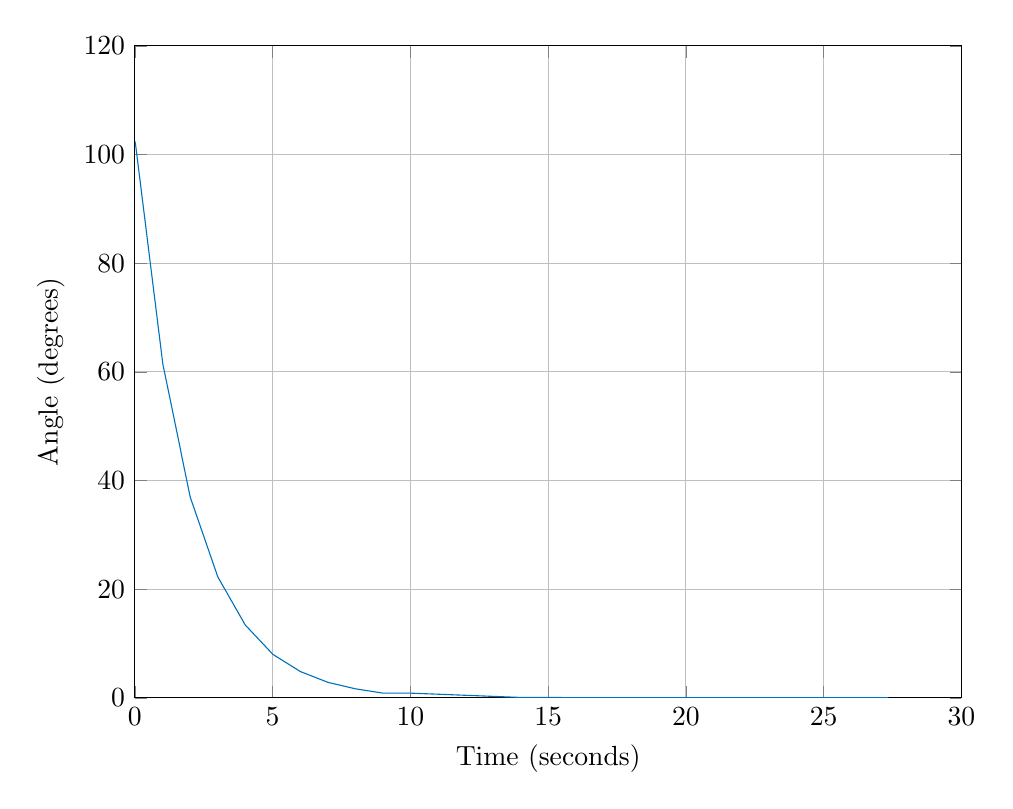
\begin{tikzpicture}

\begin{axis}[%
width=4.133in,
height=3.26in,
at={(0.693in,0.44in)},
scale only axis,
xmin=0,
xmax=30,
xmajorgrids,
xlabel={Time (seconds)},
ymin=0,
ymax=120,
ymajorgrids,
ylabel={Angle (degrees)},
axis background/.style={fill=white}
]
\addplot [color=mycolor1,solid,forget plot]
  table[row sep=crcr]{%
0	102.4204\\
0.017486686999999	102.0764\\
0.0335484049999993	101.5204\\
0.0489735169999991	100.8684\\
0.0654204590000007	100.2164\\
0.0807954470000006	99.5864\\
0.095984534	98.9524\\
0.111819789999999	98.3164\\
0.127794892999999	97.6704\\
0.143809515000999	96.9884\\
0.159864158	96.3404\\
0.176264448000001	95.6824\\
0.191918061000001	95.0424\\
0.208229863	94.3924\\
0.22411426	93.7404\\
0.240030810000001	93.0884\\
0.255976952	92.4244\\
0.271988863	91.7784\\
0.288005780999999	91.1324\\
0.303815257999999	90.4804\\
0.319800566	89.8204\\
0.335802525001001	89.1724\\
0.351768663999999	88.5224\\
0.36785526	87.8644\\
0.383954799000001	87.2124\\
0.399951771	86.5604\\
0.415880339	85.9044\\
0.431894845999999	85.2524\\
0.447974014	84.5964\\
0.463848232999999	83.9444\\
0.480008339	83.2904\\
0.495993414999001	82.6424\\
0.511988127	81.9884\\
0.528026147001	81.3044\\
0.543979419999	80.6604\\
0.560134905999999	80.0144\\
0.576019073000001	79.3664\\
0.591895217	78.7164\\
0.607847277000001	78.0684\\
0.623834802999999	77.4204\\
0.639813487999	76.7684\\
0.655864687999999	76.1144\\
0.671844843	75.4464\\
0.687894173	74.8024\\
0.703960452998999	74.1524\\
0.719861596999001	73.5004\\
0.735862183	72.8444\\
0.751862538000001	72.1984\\
0.767889197000999	71.5404\\
0.783981379999001	70.8804\\
0.799994904999999	70.2244\\
0.815962780998999	69.5724\\
0.831992070999	68.9244\\
0.847937220999999	68.2684\\
0.863962322000001	67.6104\\
0.879972584000001	66.9644\\
0.896016072000001	66.3124\\
0.912088118999999	65.6624\\
0.927922307	65.0024\\
0.944023716	64.3504\\
0.959994168	63.6924\\
0.975991230999	63.0464\\
0.992029912	62.3884\\
1.00793084	61.7084\\
1.023850434	61.1864\\
1.039763124	60.8124\\
1.055901442	60.4364\\
1.071836404	60.0384\\
1.087869267	59.6484\\
1.10386867	59.2424\\
1.119916358	58.8524\\
1.1358229	58.4684\\
1.15185658	58.0844\\
1.167908877	57.6904\\
1.183846768001	57.3004\\
1.199820039001	56.9044\\
1.215989863	56.5104\\
1.232047372	56.1184\\
1.248097771	55.7264\\
1.264938424	55.3264\\
1.280224831001	54.9384\\
1.295854792	54.5524\\
1.311873158	54.1604\\
1.327965721999	53.7644\\
1.343997818	53.3684\\
1.359990541	52.9744\\
1.375953205	52.5824\\
1.391990664	52.1884\\
1.407983296	51.7924\\
1.42398526	51.3964\\
1.439988907	51.0044\\
1.455918365999	50.6124\\
1.471983127	50.2244\\
1.487986744	49.8284\\
1.50410443	49.4324\\
1.519856507	49.0364\\
1.536033372	48.6504\\
1.551946803	48.2584\\
1.568102883	47.8624\\
1.583845648999	47.4664\\
1.599816938	47.0744\\
1.615792371001	46.6844\\
1.631799331	46.2924\\
1.647803028	45.8964\\
1.663927058	45.5064\\
1.680189577	45.0044\\
1.695951467	44.6164\\
1.711980451	44.2304\\
1.727964409	43.8364\\
1.744002825	43.4424\\
1.760010982999	43.0484\\
1.775946896	42.6504\\
1.79184524	42.2644\\
1.807861806	41.8704\\
1.823847002	41.4804\\
1.839834533	41.0844\\
1.855985263	40.6864\\
1.872113578	40.2984\\
1.887788602	39.9044\\
1.904080431	39.5144\\
1.919815951	39.1184\\
1.936070287999	38.7264\\
1.95185823	38.3324\\
1.967838134	37.9364\\
1.983960635	37.5464\\
2.000025140001	37.1644\\
2.017650045	36.8024\\
2.033143887	36.5844\\
2.048642751	36.3584\\
2.064027737	36.1244\\
2.079982323	35.9004\\
2.096419011999	35.6684\\
2.11211212	35.4264\\
2.127943664	35.1964\\
2.144116339	34.9644\\
2.1600051	34.7304\\
2.175997858	34.4924\\
2.191989798	34.2584\\
2.207913897	34.0164\\
2.22381201	33.7864\\
2.239988593001	33.5544\\
2.25599238	33.3124\\
2.272004612	33.0704\\
2.287857763001	32.8404\\
2.303951063999	32.6084\\
2.319942919	32.3804\\
2.335980313	32.1444\\
2.352239169	31.9104\\
2.368013311	31.6744\\
2.38401129	31.4404\\
2.400130168	31.2044\\
2.415943846	30.9704\\
2.431985569	30.7324\\
2.448257389	30.5024\\
2.463981428001	30.2644\\
2.479988824	30.0384\\
2.495996796	29.7984\\
2.512120174	29.5624\\
2.528009412	29.3284\\
2.543985026	29.0944\\
2.560078320999	28.8584\\
2.575957309	28.6264\\
2.592038575	28.3924\\
2.608019255	28.1584\\
2.623982851	27.9204\\
2.639868857001	27.6864\\
2.655847989001	27.4544\\
2.672064518	27.2224\\
2.687855789	26.9844\\
2.703825219	26.7484\\
2.719867364	26.5164\\
2.735848425	26.2824\\
2.751841428	26.0484\\
2.767796685999	25.8104\\
2.783994127	25.5784\\
2.799976426	25.3444\\
2.815987054	25.1044\\
2.831971804	24.8704\\
2.847952003	24.6364\\
2.864066180001	24.4044\\
2.880101629999	24.1704\\
2.896000037999	23.9324\\
2.9119947	23.7004\\
2.928207542	23.4644\\
2.943964816	23.2224\\
2.959980711001	22.9904\\
2.975975097	22.7544\\
2.991968672	22.5244\\
3.008049589	22.2904\\
3.025705628001	22.1144\\
3.041302558	21.9724\\
3.056294674	21.8384\\
3.071707325	21.7024\\
3.087762018	21.5644\\
3.10588222	21.4184\\
3.120848061	21.2764\\
3.136017734	21.1364\\
3.151834834	20.9944\\
3.168017411001	20.8504\\
3.183817157	20.7104\\
3.199883506	20.5684\\
3.215999618	20.4284\\
3.231906530999	20.2824\\
3.247868268	20.1444\\
3.263899598999	20.0024\\
3.279850943	19.8624\\
3.295889188	19.7204\\
3.311824488	19.5784\\
3.330103953	19.4284\\
3.34520471	19.2884\\
3.360502328	19.1444\\
3.376507724	19.0044\\
3.391998727	18.8624\\
3.407956905	18.7204\\
3.423716052	18.5824\\
3.439988605	18.4344\\
3.455983166001	18.2924\\
3.471984804	18.1484\\
3.487860982001	18.0104\\
3.506367524	17.8664\\
3.521821832	17.7244\\
3.536967627	17.5824\\
3.552019848001	17.4404\\
3.567876423001	17.3044\\
3.583855765	17.1604\\
3.600034659001	17.0184\\
3.616012623	16.8724\\
3.631974646	16.7324\\
3.64803659	16.5904\\
3.664004502	16.4504\\
3.679872690999	16.3044\\
3.696085323	16.1644\\
3.712132148	16.0224\\
3.728065185	15.8824\\
3.743841969	15.7384\\
3.759840189	15.5924\\
3.775891353999	15.4504\\
3.791852299	15.3104\\
3.807891971	15.1704\\
3.823991789999	15.0284\\
3.840109428	14.8844\\
3.855996638001	14.7464\\
3.871925701	14.6024\\
3.888081237001	14.4604\\
3.903997015001	14.3184\\
3.919870763	14.1784\\
3.936023091999	14.0344\\
3.951959091	13.8904\\
3.967990361	13.7504\\
3.983966682	13.6104\\
3.99996206	13.4704\\
4.017571706	13.3424\\
4.032651770999	13.2604\\
4.04783499	13.1764\\
4.063893371001	13.0944\\
4.079849379999	13.0084\\
4.095843952001	12.9224\\
4.111851974	12.8344\\
4.127999232	12.7484\\
4.14394607	12.6604\\
4.159921162999	12.5764\\
4.175822202999	12.4884\\
4.191831913	12.4024\\
4.20800091	12.3144\\
4.223868114001	12.2324\\
4.239983184	12.1464\\
4.255981995	12.0564\\
4.271850145001	11.9724\\
4.287870174	11.8844\\
4.303882005	11.8004\\
4.320301229	11.7124\\
4.335876135	11.6264\\
4.351866602	11.5424\\
4.367842502	11.4544\\
4.383905609	11.3684\\
4.399886439	11.2824\\
4.415890207	11.1984\\
4.431889204	11.1084\\
4.44789114	11.0224\\
4.463877956	10.9384\\
4.48001681	10.8504\\
4.495913405	10.7644\\
4.511827202	10.6784\\
4.527941767	10.5924\\
4.543860352	10.5044\\
4.559996389	10.4164\\
4.576008185	10.3324\\
4.591897362	10.2464\\
4.607927595001	10.1604\\
4.623936198	10.0744\\
4.639968085	9.9884\\
4.656080012	9.90239999999999\\
4.671823111	9.81439999999999\\
4.687780598	9.7304\\
4.703962403	9.64239999999999\\
4.720163187	9.55839999999999\\
4.735872136999	9.47040000000001\\
4.751936527001	9.38639999999998\\
4.767989435	9.29639999999999\\
4.783966221999	9.21040000000001\\
4.799856497	9.12239999999998\\
4.815839142	9.03639999999999\\
4.831855848999	8.95039999999999\\
4.847988704	8.86839999999999\\
4.864022178999	8.7804\\
4.879995537	8.69239999999999\\
4.895993602	8.60639999999998\\
4.912126157	8.52239999999999\\
4.928008574	8.43640000000001\\
4.944112568	8.3484\\
4.959862902	8.25839999999999\\
4.976050516	8.17439999999999\\
4.992229881999	8.0904\\
5.00798456	8.0044\\
5.025727621	7.9404\\
5.040911994	7.89439999999999\\
5.056201608	7.84439999999999\\
5.072061125	7.79239999999999\\
5.08785427	7.74239999999999\\
5.103860728	7.6944\\
5.119839359	7.64239999999999\\
5.135849677	7.5924\\
5.15183426	7.54239999999999\\
5.167928034	7.49239999999999\\
5.18420363	7.4404\\
5.200012105	7.3884\\
5.215974444	7.33840000000001\\
5.232035055001	7.28639999999999\\
5.247871685	7.23439999999999\\
5.263861435001	7.1844\\
5.279974855999	7.1344\\
5.295995893	7.08239999999999\\
5.312029757	7.0324\\
5.32800208	6.9824\\
5.343979879	6.9344\\
5.359990474	6.8844\\
5.377331107001	6.8304\\
5.392508933	6.7804\\
5.408060076	6.7304\\
5.42388316	6.6784\\
5.439875421	6.62439999999999\\
5.455980373	6.5744\\
5.471983484	6.5264\\
5.487966665	6.47439999999999\\
5.503868211001	6.4264\\
5.51998506	6.37439999999998\\
5.535943665	6.3244\\
5.551901649	6.2744\\
5.567849605	6.22439999999999\\
5.583842257	6.17440000000001\\
5.5998659	6.12439999999998\\
5.615849357	6.07039999999999\\
5.63186656	6.0164\\
5.647841391	5.96639999999999\\
5.663848662	5.91639999999998\\
5.679842938	5.86639999999998\\
5.695846786	5.8164\\
5.711855354	5.76439999999999\\
5.727846343	5.7144\\
5.74384761	5.66439999999999\\
5.759851372	5.61439999999999\\
5.775873983	5.56440000000001\\
5.791840385	5.51439999999999\\
5.807841377	5.4644\\
5.823852486	5.41239999999999\\
5.839893136999	5.3604\\
5.855842155	5.31039999999999\\
5.871846494	5.25840000000001\\
5.887839251999	5.20840000000001\\
5.903850416001	5.1544\\
5.919859576	5.10439999999998\\
5.935856994	5.0544\\
5.951836722	5.0044\\
5.967980768	4.95440000000001\\
5.98396902	4.9044\\
5.999988959	4.85439999999998\\
6.017461794	4.80839999999999\\
6.032542141	4.7784\\
6.047851054	4.74839999999998\\
6.063789746	4.7184\\
6.079982419	4.68639999999999\\
6.096028804	4.6524\\
6.112197169	4.62239999999998\\
6.127987843999	4.5904\\
6.14400659	4.55839999999999\\
6.160620305	4.5284\\
6.175926587	4.49639999999998\\
6.191874924	4.4624\\
6.207853971	4.43039999999999\\
6.223858966	4.4004\\
6.239991129	4.36839999999998\\
6.255961035	4.33840000000001\\
6.271965805	4.3044\\
6.287855514	4.2724\\
6.303849871	4.24039999999999\\
6.319843220001	4.21040000000001\\
6.335992677	4.17639999999999\\
6.352068348	4.14439999999999\\
6.367996268999	4.11239999999999\\
6.383986896	4.08239999999999\\
6.399983683	4.0504\\
6.415981171	4.02040000000001\\
6.432326658	3.98839999999998\\
6.448015282	3.95840000000001\\
6.463933515	3.92439999999999\\
6.479989165	3.89239999999999\\
6.495996857	3.8604\\
6.511966723	3.8284\\
6.527969363	3.79839999999999\\
6.543976087	3.76840000000001\\
6.560117987001	3.73439999999999\\
6.576019849	3.70039999999999\\
6.591898213001	3.6704\\
6.60800549	3.6404\\
6.623987182	3.60839999999999\\
6.639978992999	3.57639999999999\\
6.655979738	3.5424\\
6.671970694	3.5104\\
6.687890725	3.4804\\
6.703959956	3.44839999999999\\
6.719903061	3.41839999999999\\
6.736118653	3.3884\\
6.751990346	3.3524\\
6.767856928	3.32039999999999\\
6.783841984	3.29040000000001\\
6.800109087	3.25840000000001\\
6.815839205	3.22839999999999\\
6.83184929	3.1964\\
6.84785296	3.16239999999999\\
6.863820206	3.13040000000001\\
6.879848282	3.10040000000001\\
6.896027948	3.0684\\
6.912100356	3.0384\\
6.927857114	3.0064\\
6.94401239	2.97239999999999\\
6.960079546	2.9404\\
6.975990438	2.9104\\
6.991984544	2.87839999999998\\
7.007979692001	2.8484\\
7.023862178001	2.8244\\
7.039860893001	2.80439999999999\\
7.055952778	2.7884\\
7.07198731	2.76840000000001\\
7.08787378	2.75039999999998\\
7.104000367999	2.7304\\
7.119878782	2.71040000000001\\
7.135843636	2.6904\\
7.151983467	2.6724\\
7.167992752	2.6544\\
7.183983109	2.63640000000001\\
7.199993135	2.61639999999998\\
7.215927987	2.5964\\
7.231990959	2.5784\\
7.248110008	2.56039999999999\\
7.263994520001	2.54040000000001\\
7.279978317	2.52040000000001\\
7.29598012	2.50039999999998\\
7.311967852	2.4824\\
7.327984884	2.4624\\
7.344036841	2.4464\\
7.359991648	2.42639999999999\\
7.375941638001	2.40639999999999\\
7.391957109	2.3884\\
7.407991825	2.37039999999999\\
7.423983791001	2.35040000000001\\
7.440299411001	2.3304\\
7.455997626001	2.31039999999999\\
7.472022897001	2.29040000000001\\
7.487877721	2.2744\\
7.503976749999	2.25639999999999\\
7.519847844	2.23639999999999\\
7.535793886999	2.21639999999999\\
7.551727271	2.20039999999999\\
7.567746317	2.18039999999999\\
7.583805196	2.1604\\
7.599885973	2.1404\\
7.616033161001	2.12039999999999\\
7.631984665	2.10040000000001\\
7.648047667	2.08439999999999\\
7.66399407	2.06440000000001\\
7.679875387	2.04639999999999\\
7.695933044	2.0224\\
7.711983202	2.00439999999999\\
7.727866161001	1.98639999999999\\
7.743846445	1.96639999999999\\
7.759983444001	1.9464\\
7.776080985	1.92639999999999\\
7.792035334999	1.90639999999999\\
7.808116768	1.8884\\
7.824087381	1.87039999999999\\
7.839867387	1.85039999999999\\
7.855851194	1.83239999999999\\
7.871966544	1.81440000000001\\
7.887853167	1.79639999999999\\
7.904021978	1.7764\\
7.919860643001	1.75640000000001\\
7.935857589	1.73639999999999\\
7.951844027	1.71639999999999\\
7.967842142	1.6964\\
7.983788231	1.68040000000001\\
7.999854768999	1.66239999999999\\
8.017226094	1.64239999999999\\
8.03242936	1.6324\\
8.048033415	1.62039999999999\\
8.064008172	1.6104\\
8.079984532999	1.59639999999999\\
8.096111955	1.58239999999999\\
8.111885089999	1.57039999999999\\
8.127851588	1.55839999999999\\
8.143970061	1.5444\\
8.159966487	1.5324\\
8.175972364001	1.52040000000001\\
8.191934654001	1.50840000000001\\
8.207990388	1.49239999999999\\
8.22399195	1.4824\\
8.239967028	1.4704\\
8.255991984	1.45840000000001\\
8.271880347	1.4404\\
8.288003969	1.43039999999999\\
8.303895738	1.4204\\
8.319890578	1.40639999999999\\
8.335951235999	1.39239999999999\\
8.351928202999	1.38040000000001\\
8.367844089	1.36839999999998\\
8.383987025	1.3524\\
8.400064459	1.3424\\
8.415987574001	1.3304\\
8.431715610999	1.3184\\
8.447955805001	1.30239999999999\\
8.46409959	1.29040000000001\\
8.479920212	1.2804\\
8.49595922	1.26840000000001\\
8.511975155	1.25039999999998\\
8.527807334	1.24039999999999\\
8.543956756	1.22839999999999\\
8.559932374999	1.2144\\
8.575968185	1.2024\\
8.591881277	1.1904\\
8.607929852	1.1784\\
8.623839445	1.16239999999999\\
8.639833406	1.1524\\
8.65585092	1.1384\\
8.671917865	1.12839999999998\\
8.687842158	1.11239999999999\\
8.704015207	1.10040000000001\\
8.719831747	1.0904\\
8.73599239	1.07640000000001\\
8.752517784001	1.0624\\
8.768091072	1.0504\\
8.784067327	1.0384\\
8.800030593001	1.0224\\
8.815993513	1.0124\\
8.832163016	1.00039999999998\\
8.847965497	0.988399999999984\\
8.863975243	0.972399999999993\\
8.879895853	0.960400000000007\\
8.896028878001	0.950399999999988\\
8.911957110001	0.938400000000001\\
8.927983173	0.922399999999996\\
8.943893871001	0.910399999999996\\
8.959987576	0.898400000000009\\
8.975998971	0.886400000000009\\
8.992018459	0.872399999999999\\
9.007844945	0.862399999999994\\
9.025491622	0.856399999999994\\
9.040655504	0.856399999999994\\
9.05585089	0.856399999999994\\
9.071831285	0.856399999999994\\
9.087846854	0.856399999999994\\
9.103835227	0.856399999999994\\
9.119997669	0.856399999999994\\
9.13599966	0.856399999999994\\
9.151983379999	0.856399999999994\\
9.167836060001	0.856399999999994\\
9.183965129	0.856399999999994\\
9.199993144	0.856399999999994\\
9.21585087	0.856399999999994\\
9.231846695	0.856399999999994\\
9.24799586	0.856399999999994\\
9.263971531	0.856399999999994\\
9.27998909	0.856399999999994\\
9.296005692	0.856399999999994\\
9.312029775	0.856399999999994\\
9.327963308	0.856399999999994\\
9.343974773	0.856399999999994\\
9.359985577	0.856399999999994\\
9.376000405	0.856399999999994\\
9.392563669	0.856399999999994\\
9.407995697001	0.856399999999994\\
9.423989913	0.856399999999994\\
9.44008832	0.856399999999994\\
9.455951188	0.856399999999994\\
9.471966218	0.856399999999994\\
9.48797065	0.856399999999994\\
9.503844253	0.856399999999994\\
9.520148461	0.856399999999994\\
9.536045297	0.856399999999994\\
9.553297377	0.856399999999994\\
9.568767485	0.856399999999994\\
9.584163717	0.856399999999994\\
9.600208683	0.856399999999994\\
9.615995278	0.856399999999994\\
9.632013268	0.856399999999994\\
9.647977641	0.856399999999994\\
9.663963448	0.856399999999994\\
9.680035245	0.856399999999994\\
9.696007496001	0.856399999999994\\
9.711999838	0.856399999999994\\
9.727993923	0.856399999999994\\
9.744061065	0.856399999999994\\
9.760017875	0.856399999999994\\
9.776223054	0.856399999999994\\
9.792048017	0.856399999999994\\
9.807948174999	0.856399999999994\\
9.823957148999	0.856399999999994\\
9.839880228999	0.856399999999994\\
9.855805168	0.856399999999994\\
9.871788309	0.856399999999994\\
9.887849892	0.856399999999994\\
9.903951436	0.856399999999994\\
9.919780925	0.856399999999994\\
9.935843455	0.856399999999994\\
9.952036546	0.856399999999994\\
9.967985144	0.856399999999994\\
9.9840059	0.856399999999994\\
10.000018628	0.856399999999994\\
10.017668344	0.856399999999994\\
10.033358506	0.854399999999998\\
10.048801532999	0.850400000000008\\
10.063992134	0.846399999999988\\
10.079961859	0.844399999999993\\
10.096000586	0.842399999999998\\
10.111954488	0.836399999999998\\
10.127834398	0.834399999999988\\
10.144004251	0.834399999999988\\
10.159905171001	0.826400000000007\\
10.175990233	0.826400000000007\\
10.191972571	0.824399999999997\\
10.207959466001	0.816400000000002\\
10.223868092	0.816400000000002\\
10.239857909	0.814400000000006\\
10.255848978	0.806399999999982\\
10.271971805	0.806399999999982\\
10.287994816	0.804399999999987\\
10.303905493	0.800399999999996\\
10.319956954	0.796399999999991\\
10.335998406	0.794399999999996\\
10.351968337	0.790399999999991\\
10.367869703	0.786399999999986\\
10.383860541	0.784399999999991\\
10.399866719	0.782399999999996\\
10.415861216001	0.776399999999995\\
10.432036196	0.7744\\
10.448021021	0.772400000000005\\
10.463938207	0.766400000000004\\
10.480249577001	0.766400000000004\\
10.496029262	0.764399999999995\\
10.511966554	0.756399999999985\\
10.528000834999	0.756399999999985\\
10.543984898	0.75439999999999\\
10.559988415	0.74639999999998\\
10.576110942	0.74639999999998\\
10.592011831	0.744399999999985\\
10.60798081	0.738399999999984\\
10.623987157999	0.736399999999989\\
10.639983234	0.734399999999994\\
10.655962586001	0.730400000000003\\
10.672021563	0.726399999999998\\
10.68785515	0.724400000000003\\
10.703839729	0.722400000000007\\
10.72001495	0.716399999999993\\
10.736290253	0.714399999999998\\
10.752002325	0.712400000000002\\
10.767928587	0.706400000000002\\
10.78396365	0.704399999999993\\
10.800014529001	0.702399999999997\\
10.815968128	0.696399999999997\\
10.831995911	0.696399999999997\\
10.847990132	0.694400000000002\\
10.864021076	0.686400000000006\\
10.879858917	0.686400000000006\\
10.895994147	0.684400000000011\\
10.912003758999	0.676399999999987\\
10.927812883	0.676399999999987\\
10.944089962	0.674399999999991\\
10.960012951	0.670400000000001\\
10.975967372	0.666399999999996\\
10.994437291	0.664399999999986\\
11.009855928	0.6584\\
11.024862852	0.656399999999991\\
11.040363161001	0.654399999999995\\
11.055893209	0.6524\\
11.071954883	0.6464\\
11.08799588	0.64439999999999\\
11.103866797	0.642399999999995\\
11.119979726	0.636400000000009\\
11.135979645	0.634399999999999\\
11.152036092	0.634399999999999\\
11.167860453	0.62639999999999\\
11.183752573	0.62639999999999\\
11.199759137	0.624399999999994\\
11.215828492999	0.616399999999985\\
11.231808772	0.616399999999985\\
11.250404881999	0.614399999999989\\
11.265866270999	0.608399999999989\\
11.281521764	0.606399999999994\\
11.296757813	0.604399999999998\\
11.311903121001	0.600400000000008\\
11.327865785	0.596399999999988\\
11.343986763	0.594399999999993\\
11.359975071	0.592399999999998\\
11.376366240999	0.586399999999998\\
11.392050157	0.584399999999988\\
11.407961721	0.582399999999993\\
11.423941196	0.576400000000007\\
11.439990165	0.574399999999997\\
11.455954879	0.574399999999997\\
11.472048105001	0.566400000000002\\
11.487916396	0.566400000000002\\
11.503695352	0.564400000000006\\
11.521699371	0.556399999999982\\
11.536536236	0.556399999999982\\
11.551689432	0.554399999999987\\
11.569768705	0.546399999999991\\
11.584946473001	0.546399999999991\\
11.600190114001	0.544399999999996\\
11.615752999999	0.540399999999991\\
11.631693449999	0.536399999999986\\
11.647688898999	0.534399999999991\\
11.663683103	0.5304\\
11.681889187001	0.526399999999995\\
11.697101984	0.5244\\
11.712128372	0.522400000000005\\
11.727860143	0.516400000000004\\
11.743847957	0.514399999999995\\
11.759921565999	0.5124\\
11.775981921	0.506399999999985\\
11.791976771	0.50439999999999\\
11.80795432	0.50439999999999\\
11.824044034	0.49639999999998\\
11.839996891	0.49639999999998\\
11.856056169	0.494399999999985\\
11.872050741	0.486399999999989\\
11.888032609	0.486399999999989\\
11.903815577	0.484399999999994\\
11.919827874	0.478399999999993\\
11.935811235	0.476399999999998\\
11.951821115999	0.474400000000003\\
11.967815132	0.470400000000012\\
11.983844497	0.466399999999993\\
11.99986148	0.464399999999998\\
12.017454397001	0.458399999999997\\
12.032719391	0.456400000000002\\
12.048030129	0.454399999999993\\
12.06400678	0.452399999999997\\
12.079982388999	0.446399999999997\\
12.095891701	0.444400000000002\\
12.111777777	0.442399999999992\\
12.127842794999	0.436400000000006\\
12.143991495	0.436400000000006\\
12.160025336	0.434400000000011\\
12.175987049	0.426399999999987\\
12.191947357	0.426399999999987\\
12.208013426	0.424399999999991\\
12.223962285	0.416399999999996\\
12.239861184	0.416399999999996\\
12.255963174999	0.414399999999986\\
12.27186019	0.4084\\
12.287836821	0.406399999999991\\
12.303870627	0.404399999999995\\
12.319859446	0.400399999999991\\
12.33582852	0.3964\\
12.351935486	0.39439999999999\\
12.36785407	0.392399999999995\\
12.383869876	0.386400000000009\\
12.399881065	0.384399999999999\\
12.415860973	0.382400000000004\\
12.431885087	0.37639999999999\\
12.447991928	0.374399999999994\\
12.463975985999	0.374399999999994\\
12.479967546001	0.366399999999985\\
12.49600742	0.366399999999985\\
12.512026683001	0.364399999999989\\
12.527979592	0.356399999999994\\
12.543979208	0.356399999999994\\
12.560080973	0.354399999999998\\
12.575893131	0.348399999999998\\
12.591957772001	0.346399999999988\\
12.607991342	0.344399999999993\\
12.623822784	0.340399999999988\\
12.639977123	0.336399999999998\\
12.655959401	0.334399999999988\\
12.671949513	0.332399999999993\\
12.687982597	0.326400000000007\\
12.704035315	0.324399999999997\\
12.720021768	0.322400000000002\\
12.736016075	0.316400000000002\\
12.751875165	0.314400000000006\\
12.767797132	0.312399999999982\\
12.783836501	0.306399999999982\\
12.800182779	0.306399999999982\\
12.816031766	0.304399999999987\\
12.831965990999	0.296399999999991\\
12.848031032	0.296399999999991\\
12.86399961	0.294399999999996\\
12.879938294999	0.286399999999986\\
12.895996756	0.286399999999986\\
12.912105462	0.284399999999991\\
12.92792629	0.2804\\
12.943839041	0.276399999999995\\
12.959855833	0.2744\\
12.976032022	0.270399999999995\\
12.99201621	0.266400000000004\\
13.007858497	0.264399999999995\\
13.023792321	0.2624\\
13.039744899	0.256399999999985\\
13.05591623	0.25439999999999\\
13.071846596	0.252399999999994\\
13.087981905999	0.24639999999998\\
13.103950594	0.24639999999998\\
13.120117336	0.244399999999985\\
13.136024737	0.236399999999989\\
13.151997252	0.236399999999989\\
13.167858489	0.234399999999994\\
13.183939222	0.226399999999998\\
13.199923226	0.226399999999998\\
13.215962118	0.224400000000003\\
13.231953358	0.218400000000003\\
13.248001446	0.216399999999993\\
13.263987298001	0.214399999999998\\
13.279980055	0.210399999999993\\
13.296214871	0.206400000000002\\
13.312134383001	0.204399999999993\\
13.328006872999	0.202399999999997\\
13.343871655999	0.196399999999997\\
13.359846959	0.194400000000002\\
13.376176419	0.192399999999992\\
13.391998771	0.186400000000006\\
13.407951793	0.184400000000011\\
13.423934056999	0.184400000000011\\
13.440016056999	0.176399999999987\\
13.455928718001	0.176399999999987\\
13.47200945	0.174399999999991\\
13.487994726	0.166399999999996\\
13.503930695	0.166399999999996\\
13.520122669	0.164399999999986\\
13.535994387	0.156399999999991\\
13.552143063	0.156399999999991\\
13.567978359	0.154399999999995\\
13.583843648	0.150399999999991\\
13.599871936	0.1464\\
13.615848983	0.14439999999999\\
13.632066635	0.1404\\
13.648000169	0.136400000000009\\
13.663961109	0.134399999999999\\
13.679905552	0.132400000000004\\
13.695858747999	0.12639999999999\\
13.711932391	0.124399999999994\\
13.72796795	0.122399999999999\\
13.743951187001	0.116399999999985\\
13.759979856	0.114399999999989\\
13.776030564	0.114399999999989\\
13.7920226	0.106399999999994\\
13.807942248	0.106399999999994\\
13.823999681999	0.104399999999998\\
13.84001694	0.0963999999999885\\
13.856214341001	0.0963999999999885\\
13.872008414	0.0943999999999932\\
13.887983235	0.0883999999999929\\
13.903994861	0.0863999999999976\\
13.919937625	0.084399999999988\\
13.936033271	0.0803999999999974\\
13.951986549	0.0764000000000067\\
13.967998911001	0.0743999999999971\\
13.983962302	0.0724000000000018\\
13.999994825	0.0664000000000016\\
14.017505371001	0.0664000000000016\\
14.032585284999	0.0664000000000016\\
14.047964185	0.0664000000000016\\
14.063867397001	0.0664000000000016\\
14.080146228	0.0664000000000016\\
14.095993591	0.0664000000000016\\
14.111979188	0.0664000000000016\\
14.127994191	0.0664000000000016\\
14.143957306	0.0664000000000016\\
14.159874658	0.0664000000000016\\
14.175938191	0.0664000000000016\\
14.191981277	0.0664000000000016\\
14.207869819001	0.0664000000000016\\
14.223915171	0.0664000000000016\\
14.239848654	0.0664000000000016\\
14.255865086	0.0664000000000016\\
14.271942861	0.0664000000000016\\
14.288025542	0.0664000000000016\\
14.303891578	0.0664000000000016\\
14.319946526	0.0664000000000016\\
14.336028761	0.0664000000000016\\
14.351872246	0.0664000000000016\\
14.367987801999	0.0664000000000016\\
14.384143343001	0.0664000000000016\\
14.399955962	0.0664000000000016\\
14.415984035	0.0664000000000016\\
14.431957684	0.0664000000000016\\
14.448025066	0.0664000000000016\\
14.463973187	0.0664000000000016\\
14.480037472	0.0664000000000016\\
14.495865577	0.0664000000000016\\
14.512023894	0.0664000000000016\\
14.527988935	0.0664000000000016\\
14.544015689	0.0664000000000016\\
14.559991834	0.0664000000000016\\
14.575987177	0.0664000000000016\\
14.591970228	0.0664000000000016\\
14.607939893999	0.0664000000000016\\
14.623969289	0.0664000000000016\\
14.640000322999	0.0664000000000016\\
14.656042072	0.0664000000000016\\
14.671992744001	0.0664000000000016\\
14.68785877	0.0664000000000016\\
14.703814629	0.0664000000000016\\
14.719799759	0.0664000000000016\\
14.735826303	0.0664000000000016\\
14.751810757	0.0664000000000016\\
14.767883837	0.0664000000000016\\
14.784403879	0.0664000000000016\\
14.799988823	0.0664000000000016\\
14.815851666	0.0664000000000016\\
14.831857779	0.0664000000000016\\
14.847833027001	0.0664000000000016\\
14.863882498	0.0664000000000016\\
14.879853897	0.0664000000000016\\
14.895881478	0.0664000000000016\\
14.911957279	0.0664000000000016\\
14.928018539	0.0664000000000016\\
14.944133376	0.0664000000000016\\
14.959996134	0.0664000000000016\\
14.97601438	0.0664000000000016\\
14.991969301999	0.0664000000000016\\
15.007964845	0.0664000000000016\\
15.025661518	0.0664000000000016\\
15.040820341	0.0644000000000062\\
15.056224806	0.0644000000000062\\
15.071796811	0.0644000000000062\\
15.08784769	0.0644000000000062\\
15.103984965	0.0623999999999967\\
15.120584066	0.0623999999999967\\
15.136154065999	0.0623999999999967\\
15.15209219	0.0604000000000013\\
15.167991652	0.0604000000000013\\
15.183706164001	0.0604000000000013\\
15.201759735	0.058400000000006\\
15.217388007	0.058400000000006\\
15.232905603	0.058400000000006\\
15.248296016	0.0563999999999822\\
15.263963767	0.0563999999999822\\
15.280054823	0.0563999999999822\\
15.296020414001	0.0543999999999869\\
15.311987974	0.0543999999999869\\
15.328046937	0.0543999999999869\\
15.343970919	0.0523999999999916\\
15.359881395	0.0523999999999916\\
15.375884486	0.0523999999999916\\
15.391968254	0.0523999999999916\\
15.407997786	0.0503999999999962\\
15.424042336	0.0503999999999962\\
15.439856964999	0.0503999999999962\\
15.456127652001	0.0483999999999867\\
15.471978052	0.0483999999999867\\
15.487966064	0.0483999999999867\\
15.503843471	0.0463999999999913\\
15.519966161	0.0463999999999913\\
15.535982535	0.0463999999999913\\
15.551979686	0.044399999999996\\
15.568175523999	0.044399999999996\\
15.583861907	0.044399999999996\\
15.599826639	0.0424000000000007\\
15.615854448	0.0424000000000007\\
15.631846093	0.0424000000000007\\
15.647848268	0.0404000000000053\\
15.663838434	0.0404000000000053\\
15.679902148	0.0404000000000053\\
15.696025843001	0.0404000000000053\\
15.711890284	0.0383999999999958\\
15.727964952	0.0383999999999958\\
15.743914416001	0.0383999999999958\\
15.760064105	0.0364000000000004\\
15.775993890001	0.0364000000000004\\
15.791955356	0.0364000000000004\\
15.80799266	0.0344000000000051\\
15.823964861	0.0344000000000051\\
15.839869749	0.0344000000000051\\
15.855842507	0.0324000000000098\\
15.871849867999	0.0324000000000098\\
15.88790435	0.0324000000000098\\
15.904392189	0.030399999999986\\
15.919982515001	0.030399999999986\\
15.935988683	0.030399999999986\\
15.951957441	0.0283999999999907\\
15.967857509	0.0283999999999907\\
15.983846212	0.0283999999999907\\
15.999962339	0.0263999999999953\\
16.017517646	0.0263999999999953\\
16.032688442	0.0263999999999953\\
16.048149896	0.0263999999999953\\
16.064113332999	0.0263999999999953\\
16.080008785	0.0263999999999953\\
16.095961627	0.0263999999999953\\
16.112004764	0.0263999999999953\\
16.127964431999	0.0263999999999953\\
16.143976628	0.0263999999999953\\
16.160000321	0.0263999999999953\\
16.17607249	0.0263999999999953\\
16.191987274	0.0263999999999953\\
16.208037217	0.0263999999999953\\
16.22399262	0.0263999999999953\\
16.239877232	0.0263999999999953\\
16.255945610999	0.0263999999999953\\
16.271848865999	0.0263999999999953\\
16.28784699	0.0263999999999953\\
16.303847586	0.0263999999999953\\
16.319818905	0.0263999999999953\\
16.335847704	0.0263999999999953\\
16.352030929	0.0263999999999953\\
16.367970390001	0.0263999999999953\\
16.383715136	0.0263999999999953\\
16.399728560001	0.0263999999999953\\
16.415784848001	0.0263999999999953\\
16.431910035	0.0263999999999953\\
16.447990225	0.0263999999999953\\
16.463950805	0.0263999999999953\\
16.479734909	0.0263999999999953\\
16.495704999	0.0263999999999953\\
16.513856678	0.0263999999999953\\
16.52875146	0.0263999999999953\\
16.543922847	0.0263999999999953\\
16.560009081	0.0263999999999953\\
16.576072243	0.0263999999999953\\
16.59196082	0.0263999999999953\\
16.607864129999	0.0263999999999953\\
16.623845196	0.0263999999999953\\
16.639820183999	0.0263999999999953\\
16.655829082	0.0263999999999953\\
16.671829252	0.0263999999999953\\
16.687915456	0.0263999999999953\\
16.703969924	0.0263999999999953\\
16.719966269	0.0263999999999953\\
16.735964615	0.0263999999999953\\
16.751957543	0.0263999999999953\\
16.767959055001	0.0263999999999953\\
16.783785306	0.0263999999999953\\
16.799734558999	0.0263999999999953\\
16.815733957	0.0263999999999953\\
16.833800629	0.0263999999999953\\
16.848679415	0.0263999999999953\\
16.863706291	0.0263999999999953\\
16.881760272	0.0263999999999953\\
16.896666697001	0.0263999999999953\\
16.911775562001	0.0263999999999953\\
16.927722907	0.0263999999999953\\
16.943940587	0.0263999999999953\\
16.959902704	0.0263999999999953\\
16.975753610999	0.0263999999999953\\
16.9921274	0.0263999999999953\\
17.008000469	0.0263999999999953\\
17.025863544	0.0263999999999953\\
17.041092426	0.0263999999999953\\
17.056177337	0.0263999999999953\\
17.071869559	0.0263999999999953\\
17.087918299	0.0263999999999953\\
17.104006935	0.0263999999999953\\
17.119897072999	0.0263999999999953\\
17.135990688999	0.0263999999999953\\
17.152013084	0.0263999999999953\\
17.167959011	0.0263999999999953\\
17.183838131001	0.0263999999999953\\
17.199848980001	0.0263999999999953\\
17.21596468	0.0263999999999953\\
17.232027246	0.0263999999999953\\
17.248034041	0.0263999999999953\\
17.26396996	0.0263999999999953\\
17.279975657	0.0263999999999953\\
17.295859492	0.0263999999999953\\
17.311968058	0.0263999999999953\\
17.327984694	0.0263999999999953\\
17.343860296	0.0263999999999953\\
17.359852703	0.0263999999999953\\
17.376004651	0.0263999999999953\\
17.391890747	0.0263999999999953\\
17.407816312	0.0263999999999953\\
17.42391026	0.0263999999999953\\
17.439815258001	0.0263999999999953\\
17.455978096	0.0263999999999953\\
17.471736298001	0.0263999999999953\\
17.489935733	0.0263999999999953\\
17.504925426	0.0263999999999953\\
17.520689742	0.0263999999999953\\
17.537219983	0.0263999999999953\\
17.552052568	0.0263999999999953\\
17.567695725001	0.0263999999999953\\
17.585743891	0.0263999999999953\\
17.600662918	0.0263999999999953\\
17.616058233	0.0263999999999953\\
17.631712181	0.0263999999999953\\
17.649805993	0.0263999999999953\\
17.6647244	0.0263999999999953\\
17.679697486	0.0263999999999953\\
17.697803862001	0.0263999999999953\\
17.712675811	0.0263999999999953\\
17.727703604	0.0263999999999953\\
17.745704318	0.0263999999999953\\
17.760588605	0.0263999999999953\\
17.77569267	0.0263999999999953\\
17.793704681	0.0263999999999953\\
17.808644798	0.0263999999999953\\
17.823708869	0.0263999999999953\\
17.841774325	0.0263999999999953\\
17.856663253	0.0263999999999953\\
17.871696656	0.0263999999999953\\
17.889769353	0.0263999999999953\\
17.904684919	0.0263999999999953\\
17.919760850001	0.0263999999999953\\
17.937756297	0.0263999999999953\\
17.952573419	0.0263999999999953\\
17.967702661001	0.0263999999999953\\
17.985722971999	0.0263999999999953\\
18.00056186	0.0263999999999953\\
18.017619308	0.0263999999999953\\
18.03246994	0.0263999999999953\\
18.047725777001	0.0263999999999953\\
18.063774362001	0.0263999999999953\\
18.081891108	0.0263999999999953\\
18.097230375	0.0263999999999953\\
18.112469846999	0.0263999999999953\\
18.127907624	0.0263999999999953\\
18.143765162	0.0263999999999953\\
18.159796461	0.0263999999999953\\
18.175803470001	0.0263999999999953\\
18.193939686	0.0263999999999953\\
18.207885768	0.0263999999999953\\
18.223738921	0.0263999999999953\\
18.239895754	0.0263999999999953\\
18.255822669999	0.0263999999999953\\
18.272403217	0.0263999999999953\\
18.287829009	0.0263999999999953\\
18.30393959	0.0263999999999953\\
18.319756306	0.0263999999999953\\
18.337959949001	0.0263999999999953\\
18.352987810001	0.0263999999999953\\
18.367927133	0.0263999999999953\\
18.38382451	0.0263999999999953\\
18.399720395	0.0263999999999953\\
18.417809681	0.0263999999999953\\
18.432670225	0.0263999999999953\\
18.447838515	0.0263999999999953\\
18.463791142	0.0263999999999953\\
18.479975811	0.0263999999999953\\
18.495888361	0.0263999999999953\\
18.511961516	0.0263999999999953\\
18.527858214999	0.0263999999999953\\
18.543979428	0.0263999999999953\\
18.559893312001	0.0263999999999953\\
18.575853355999	0.0263999999999953\\
18.591852267	0.0263999999999953\\
18.607859628	0.0263999999999953\\
18.623843606	0.0263999999999953\\
18.639897752	0.0263999999999953\\
18.655996613	0.0263999999999953\\
18.671965885	0.0263999999999953\\
18.687963403	0.0263999999999953\\
18.704104852	0.0263999999999953\\
18.71988154	0.0263999999999953\\
18.735844577999	0.0263999999999953\\
18.751749129	0.0263999999999953\\
18.767761343	0.0263999999999953\\
18.783830404001	0.0263999999999953\\
18.799738565	0.0263999999999953\\
18.815954623	0.0263999999999953\\
18.832014064	0.0263999999999953\\
18.847959128	0.0263999999999953\\
18.863999118	0.0263999999999953\\
18.879987942	0.0263999999999953\\
18.896069546	0.0263999999999953\\
18.912179639	0.0263999999999953\\
18.927993396	0.0263999999999953\\
18.943971209999	0.0263999999999953\\
18.959987376001	0.0263999999999953\\
18.976096762	0.0263999999999953\\
18.991990816	0.0263999999999953\\
19.00837016	0.0263999999999953\\
19.024136915	0.0263999999999953\\
19.039973013	0.0263999999999953\\
19.055886366	0.0263999999999953\\
19.071963731	0.0263999999999953\\
19.087959921	0.0263999999999953\\
19.103970785	0.0263999999999953\\
19.119880388	0.0263999999999953\\
19.135965801	0.0263999999999953\\
19.151980433	0.0263999999999953\\
19.167970291999	0.0263999999999953\\
19.184376558999	0.0263999999999953\\
19.200135076	0.0263999999999953\\
19.215870566	0.0263999999999953\\
19.231859289	0.0263999999999953\\
19.247869326	0.0263999999999953\\
19.266232589999	0.0263999999999953\\
19.281389287	0.0263999999999953\\
19.296521419999	0.0263999999999953\\
19.311771995	0.0263999999999953\\
19.327852117	0.0263999999999953\\
19.343865992	0.0263999999999953\\
19.360196094	0.0263999999999953\\
19.376004529	0.0263999999999953\\
19.391718386	0.0263999999999953\\
19.410013238	0.0263999999999953\\
19.425320156	0.0263999999999953\\
19.440931054	0.0263999999999953\\
19.456409150999	0.0263999999999953\\
19.471845428	0.0263999999999953\\
19.487843553001	0.0263999999999953\\
19.503830287	0.0263999999999953\\
19.519884809	0.0263999999999953\\
19.535986303001	0.0263999999999953\\
19.551939708	0.0263999999999953\\
19.567995567	0.0263999999999953\\
19.583984243	0.0263999999999953\\
19.599996352	0.0263999999999953\\
19.616050418	0.0263999999999953\\
19.631867929	0.0263999999999953\\
19.647839914999	0.0263999999999953\\
19.663872558	0.0263999999999953\\
19.679829223	0.0263999999999953\\
19.695911589	0.0263999999999953\\
19.711940884	0.0263999999999953\\
19.727959892	0.0263999999999953\\
19.74401462	0.0263999999999953\\
19.759989056	0.0263999999999953\\
19.775777585	0.0263999999999953\\
19.791667472	0.0263999999999953\\
19.807666350999	0.0263999999999953\\
19.823674697	0.0263999999999953\\
19.839739436	0.0263999999999953\\
19.855661152001	0.0263999999999953\\
19.871681181	0.0263999999999953\\
19.887671569	0.0263999999999953\\
19.905883468001	0.0263999999999953\\
19.921355597	0.0263999999999953\\
19.936829629	0.0263999999999953\\
19.952205680001	0.0263999999999953\\
19.968050162	0.0263999999999953\\
19.983996735	0.0263999999999953\\
20.000027001999	0.0263999999999953\\
20.017910129	0.0263999999999953\\
20.033451207	0.0263999999999953\\
20.04868516	0.0263999999999953\\
20.064084938999	0.0263999999999953\\
20.079990319001	0.0263999999999953\\
20.095977964999	0.0263999999999953\\
20.111995218	0.0263999999999953\\
20.128131526	0.0263999999999953\\
20.143989683999	0.0263999999999953\\
20.159978207	0.0263999999999953\\
20.175972017	0.0263999999999953\\
20.19198494	0.0263999999999953\\
20.207866581	0.0263999999999953\\
20.223800746	0.0263999999999953\\
20.239961283	0.0263999999999953\\
20.255979454	0.0263999999999953\\
20.273507522001	0.0263999999999953\\
20.287962244	0.0263999999999953\\
20.304000609	0.0263999999999953\\
20.320096219	0.0263999999999953\\
20.335855664	0.0263999999999953\\
20.351874084001	0.0263999999999953\\
20.367978149	0.0263999999999953\\
20.383783703	0.0263999999999953\\
20.401827682	0.0263999999999953\\
20.416707212	0.0263999999999953\\
20.431880138	0.0263999999999953\\
20.447930686	0.0263999999999953\\
20.463844295	0.0263999999999953\\
20.479835183	0.0263999999999953\\
20.495845706	0.0263999999999953\\
20.511921096	0.0263999999999953\\
20.527785999	0.0263999999999953\\
20.543962663	0.0263999999999953\\
20.559966256	0.0263999999999953\\
20.57593645	0.0263999999999953\\
20.591972908	0.0263999999999953\\
20.60797373	0.0263999999999953\\
20.624033890001	0.0263999999999953\\
20.639914969	0.0263999999999953\\
20.655931386	0.0263999999999953\\
20.671876701	0.0263999999999953\\
20.687855126	0.0263999999999953\\
20.70385735	0.0263999999999953\\
20.719855615	0.0263999999999953\\
20.735844088001	0.0263999999999953\\
20.751865796001	0.0263999999999953\\
20.767877857001	0.0263999999999953\\
20.783880227	0.0263999999999953\\
20.799809681	0.0263999999999953\\
20.815843176	0.0263999999999953\\
20.831861903	0.0263999999999953\\
20.847868502	0.0263999999999953\\
20.863698093999	0.0263999999999953\\
20.879664898	0.0263999999999953\\
20.895660773999	0.0263999999999953\\
20.913927903	0.0263999999999953\\
20.928990644	0.0263999999999953\\
20.944062575	0.0263999999999953\\
20.959883113	0.0263999999999953\\
20.97596645	0.0263999999999953\\
20.991900109	0.0263999999999953\\
21.007984704999	0.0263999999999953\\
21.025902839	0.0263999999999953\\
21.041257822	0.0263999999999953\\
21.056469720001	0.0263999999999953\\
21.07183648	0.0263999999999953\\
21.087887495	0.0263999999999953\\
21.103923209999	0.0263999999999953\\
21.119849066	0.0263999999999953\\
21.135845562	0.0263999999999953\\
21.151873369001	0.0263999999999953\\
21.167882845	0.0263999999999953\\
21.183990051	0.0263999999999953\\
21.199931513	0.0263999999999953\\
21.215854532	0.0263999999999953\\
21.231965543	0.0263999999999953\\
21.247999834	0.0263999999999953\\
21.263992527	0.0263999999999953\\
21.280046296	0.0263999999999953\\
21.295954388999	0.0263999999999953\\
21.31197509	0.0263999999999953\\
21.327860519	0.0263999999999953\\
21.343964478	0.0263999999999953\\
21.359964341999	0.0263999999999953\\
21.375853001001	0.0263999999999953\\
21.391722498	0.0263999999999953\\
21.409801405999	0.0263999999999953\\
21.424854324	0.0263999999999953\\
21.440132298	0.0263999999999953\\
21.457224084999	0.0263999999999953\\
21.47238687	0.0263999999999953\\
21.487794565999	0.0263999999999953\\
21.50639076	0.0263999999999953\\
21.520904986	0.0263999999999953\\
21.537640012	0.0263999999999953\\
21.553210533	0.0263999999999953\\
21.568698989	0.0263999999999953\\
21.584111617	0.0263999999999953\\
21.599913658	0.0263999999999953\\
21.615960864	0.0263999999999953\\
21.631866133	0.0263999999999953\\
21.64799785	0.0263999999999953\\
21.66396042	0.0263999999999953\\
21.679854032999	0.0263999999999953\\
21.695834422	0.0263999999999953\\
21.711839172	0.0263999999999953\\
21.727991546	0.0263999999999953\\
21.743981202	0.0263999999999953\\
21.760266533	0.0263999999999953\\
21.775728627	0.0263999999999953\\
21.79166907	0.0263999999999953\\
21.807703426	0.0263999999999953\\
21.82365321	0.0263999999999953\\
21.839691584	0.0263999999999953\\
21.855711001	0.0263999999999953\\
21.871678298001	0.0263999999999953\\
21.887871279	0.0263999999999953\\
21.903849634	0.0263999999999953\\
21.919842863	0.0263999999999953\\
21.935853396	0.0263999999999953\\
21.95184474	0.0263999999999953\\
21.967850421999	0.0263999999999953\\
21.983850281	0.0263999999999953\\
21.999823795	0.0263999999999953\\
22.017495987	0.0263999999999953\\
22.03191975	0.0263999999999953\\
22.047981485	0.0263999999999953\\
22.063968441	0.0263999999999953\\
22.080108298001	0.0263999999999953\\
22.095915235999	0.0263999999999953\\
22.112149631	0.0263999999999953\\
22.127996351	0.0263999999999953\\
22.143998432	0.0263999999999953\\
22.160005898	0.0263999999999953\\
22.175971629	0.0263999999999953\\
22.191963725	0.0263999999999953\\
22.208002041	0.0263999999999953\\
22.223968118	0.0263999999999953\\
22.239855602	0.0263999999999953\\
22.255841239001	0.0263999999999953\\
22.271785287	0.0263999999999953\\
22.287943238	0.0263999999999953\\
22.303816485	0.0263999999999953\\
22.319953289	0.0263999999999953\\
22.335923832	0.0263999999999953\\
22.351964251	0.0263999999999953\\
22.36806757	0.0263999999999953\\
22.383728051	0.0263999999999953\\
22.399718245	0.0263999999999953\\
22.415694535	0.0263999999999953\\
22.431730779001	0.0263999999999953\\
22.44796406	0.0263999999999953\\
22.463968605	0.0263999999999953\\
22.479915914	0.0263999999999953\\
22.49599841	0.0263999999999953\\
22.511748671	0.0263999999999953\\
22.527983249	0.0263999999999953\\
22.544010029001	0.0263999999999953\\
22.560114584	0.0263999999999953\\
22.576016922	0.0263999999999953\\
22.59198543	0.0263999999999953\\
22.607726787999	0.0263999999999953\\
22.624040919	0.0263999999999953\\
22.64016106	0.0263999999999953\\
22.655967766	0.0263999999999953\\
22.671964652999	0.0263999999999953\\
22.687973186	0.0263999999999953\\
22.703870643	0.0263999999999953\\
22.719710519	0.0263999999999953\\
22.73780368	0.0263999999999953\\
22.753066409001	0.0263999999999953\\
22.768305207	0.0263999999999953\\
22.784014344	0.0263999999999953\\
22.799921596999	0.0263999999999953\\
22.815855126	0.0263999999999953\\
22.831852514	0.0263999999999953\\
22.847851576	0.0263999999999953\\
22.86401462	0.0263999999999953\\
22.87995112	0.0263999999999953\\
22.896080861	0.0263999999999953\\
22.912108043	0.0263999999999953\\
22.927997557	0.0263999999999953\\
22.943997846	0.0263999999999953\\
22.959998867999	0.0263999999999953\\
22.976002134	0.0263999999999953\\
22.991997306999	0.0263999999999953\\
23.008009695	0.0263999999999953\\
23.025560262	0.0263999999999953\\
23.041022205	0.0263999999999953\\
23.05635921	0.0263999999999953\\
23.071822348	0.0263999999999953\\
23.087827122999	0.0263999999999953\\
23.103740474	0.0263999999999953\\
23.11988083	0.0263999999999953\\
23.135953891	0.0263999999999953\\
23.152258669999	0.0263999999999953\\
23.168181108	0.0263999999999953\\
23.183962366	0.0263999999999953\\
23.200022256001	0.0263999999999953\\
23.215963978	0.0263999999999953\\
23.2319697	0.0263999999999953\\
23.247840767	0.0263999999999953\\
23.26604081	0.0263999999999953\\
23.28108139	0.0263999999999953\\
23.296191019	0.0263999999999953\\
23.312712297	0.0263999999999953\\
23.327843649	0.0263999999999953\\
23.343835054	0.0263999999999953\\
23.359856100001	0.0263999999999953\\
23.375945031	0.0263999999999953\\
23.391739945	0.0263999999999953\\
23.409744897001	0.0263999999999953\\
23.424652053999	0.0263999999999953\\
23.439907514	0.0263999999999953\\
23.45813677	0.0263999999999953\\
23.473112629999	0.0263999999999953\\
23.488438181	0.0263999999999953\\
23.503797264	0.0263999999999953\\
23.519696914	0.0263999999999953\\
23.53580193	0.0263999999999953\\
23.553014820999	0.0263999999999953\\
23.567958912	0.0263999999999953\\
23.583806782	0.0263999999999953\\
23.599808368	0.0263999999999953\\
23.615953561	0.0263999999999953\\
23.631741293	0.0263999999999953\\
23.647770037999	0.0263999999999953\\
23.663888720001	0.0263999999999953\\
23.679743401	0.0263999999999953\\
23.695864564	0.0263999999999953\\
23.711993758	0.0263999999999953\\
23.727962369	0.0263999999999953\\
23.743994296001	0.0263999999999953\\
23.759925959	0.0263999999999953\\
23.775739219	0.0263999999999953\\
23.791970297	0.0263999999999953\\
23.807762145	0.0263999999999953\\
23.823687945	0.0263999999999953\\
23.839681058	0.0263999999999953\\
23.855673759	0.0263999999999953\\
23.871688529	0.0263999999999953\\
23.887694525	0.0263999999999953\\
23.903762181	0.0263999999999953\\
23.919760238	0.0263999999999953\\
23.935905431999	0.0263999999999953\\
23.951835673	0.0263999999999953\\
23.967754408	0.0263999999999953\\
23.983712933	0.0263999999999953\\
23.999826187	0.0263999999999953\\
24.017461093001	0.0263999999999953\\
24.032018996	0.0263999999999953\\
24.047880739001	0.0263999999999953\\
24.063862407	0.0263999999999953\\
24.079840355	0.0263999999999953\\
24.095876487	0.0263999999999953\\
24.11201766	0.0263999999999953\\
24.128030168	0.0263999999999953\\
24.143982063	0.0263999999999953\\
24.159971739001	0.0263999999999953\\
24.175993993	0.0263999999999953\\
24.191991386	0.0263999999999953\\
24.208112159001	0.0263999999999953\\
24.223957794	0.0263999999999953\\
24.239990095	0.0263999999999953\\
24.255930223	0.0263999999999953\\
24.271741556	0.0263999999999953\\
24.28798474	0.0263999999999953\\
24.304016730999	0.0263999999999953\\
24.319983619999	0.0263999999999953\\
24.33586913	0.0263999999999953\\
24.35198441	0.0263999999999953\\
24.367977088001	0.0263999999999953\\
24.384684484	0.0263999999999953\\
24.400084379	0.0263999999999953\\
24.415795622999	0.0263999999999953\\
24.43189798	0.0263999999999953\\
24.447777122	0.0263999999999953\\
24.463730853	0.0263999999999953\\
24.479777289999	0.0263999999999953\\
24.495692033	0.0263999999999953\\
24.511714076	0.0263999999999953\\
24.527700905999	0.0263999999999953\\
24.543761357	0.0263999999999953\\
24.559748292	0.0263999999999953\\
24.575687541001	0.0263999999999953\\
24.591663573	0.0263999999999953\\
24.607687268999	0.0263999999999953\\
24.623851097	0.0263999999999953\\
24.639846024	0.0263999999999953\\
24.65587553	0.0263999999999953\\
24.671988616	0.0263999999999953\\
24.688044977	0.0263999999999953\\
24.704549815	0.0263999999999953\\
24.72012457	0.0263999999999953\\
24.735984798	0.0263999999999953\\
24.751982823	0.0263999999999953\\
24.768001328	0.0263999999999953\\
24.783917157	0.0263999999999953\\
24.799991544	0.0263999999999953\\
24.815991488	0.0263999999999953\\
24.832020723001	0.0263999999999953\\
24.848141336	0.0263999999999953\\
24.863998782	0.0263999999999953\\
24.880006338	0.0263999999999953\\
24.895971212	0.0263999999999953\\
24.912015707	0.0263999999999953\\
24.927964555	0.0263999999999953\\
24.943963808	0.0263999999999953\\
24.960144416001	0.0263999999999953\\
24.975984608	0.0263999999999953\\
24.991999556	0.0263999999999953\\
25.007854456	0.0263999999999953\\
25.025772869	0.0263999999999953\\
25.04119089	0.0263999999999953\\
25.056365651	0.0263999999999953\\
25.071863503001	0.0263999999999953\\
25.08800786	0.0263999999999953\\
25.103860268	0.0263999999999953\\
25.11999579	0.0263999999999953\\
25.13604065	0.0263999999999953\\
25.151987845001	0.0263999999999953\\
25.167845115	0.0263999999999953\\
25.183959609	0.0263999999999953\\
25.200025918	0.0263999999999953\\
25.216330923001	0.0263999999999953\\
25.231994735	0.0263999999999953\\
25.247992189	0.0263999999999953\\
25.264027878001	0.0263999999999953\\
25.279901787	0.0263999999999953\\
25.295925901	0.0263999999999953\\
25.312013548	0.0263999999999953\\
25.327854707	0.0263999999999953\\
25.343968153	0.0263999999999953\\
25.359824008	0.0263999999999953\\
25.375949599	0.0263999999999953\\
25.391853198	0.0263999999999953\\
25.407690597	0.0263999999999953\\
25.425880655	0.0263999999999953\\
25.441234381001	0.0263999999999953\\
25.456417394	0.0263999999999953\\
25.47195486	0.0263999999999953\\
25.4878848	0.0263999999999953\\
25.503820850001	0.0263999999999953\\
25.519921968001	0.0263999999999953\\
25.5358883	0.0263999999999953\\
25.551989445999	0.0263999999999953\\
25.568017842	0.0263999999999953\\
25.583804766	0.0263999999999953\\
25.599739006	0.0263999999999953\\
25.61585935	0.0263999999999953\\
25.631858256	0.0263999999999953\\
25.647846484	0.0263999999999953\\
25.663844183	0.0263999999999953\\
25.679842127	0.0263999999999953\\
25.695840973	0.0263999999999953\\
25.711866054	0.0263999999999953\\
25.727867361	0.0263999999999953\\
25.743864439	0.0263999999999953\\
25.759854626	0.0263999999999953\\
25.775780473001	0.0263999999999953\\
25.791849232	0.0263999999999953\\
25.807850869	0.0263999999999953\\
25.823884309	0.0263999999999953\\
25.839829657	0.0263999999999953\\
25.855857938	0.0263999999999953\\
25.871753761	0.0263999999999953\\
25.887725711001	0.0263999999999953\\
25.903740574	0.0263999999999953\\
25.921961381	0.0263999999999953\\
25.93680253	0.0263999999999953\\
25.951820852	0.0263999999999953\\
25.967797629	0.0263999999999953\\
25.983803997	0.0263999999999953\\
25.999803284	0.0263999999999953\\
26.017121259	0.0263999999999953\\
26.032117612	0.0263999999999953\\
26.047852739	0.0263999999999953\\
26.063798024	0.0263999999999953\\
26.079965101	0.0263999999999953\\
26.095988363	0.0263999999999953\\
26.111981692001	0.0263999999999953\\
26.127945795	0.0263999999999953\\
26.144018107	0.0263999999999953\\
26.159883035	0.0263999999999953\\
26.175967531	0.0263999999999953\\
26.191985513001	0.0263999999999953\\
26.208027891	0.0263999999999953\\
26.223967312	0.0263999999999953\\
26.239971215	0.0263999999999953\\
26.256012709	0.0263999999999953\\
26.271758344	0.0263999999999953\\
26.289881725001	0.0263999999999953\\
26.305306942	0.0263999999999953\\
26.320806055	0.0263999999999953\\
26.336526835	0.0263999999999953\\
26.352012132	0.0263999999999953\\
26.367965319	0.0263999999999953\\
26.384006381	0.0263999999999953\\
26.399963017	0.0263999999999953\\
26.415974176	0.0263999999999953\\
26.431964175	0.0263999999999953\\
26.447919538	0.0263999999999953\\
26.463798859	0.0263999999999953\\
26.479698734	0.0263999999999953\\
26.495681731	0.0263999999999953\\
26.511849604	0.0263999999999953\\
26.52776905	0.0263999999999953\\
26.543976905	0.0263999999999953\\
26.559962596	0.0263999999999953\\
26.576080086001	0.0263999999999953\\
26.591903085	0.0263999999999953\\
26.607889167	0.0263999999999953\\
26.623848394	0.0263999999999953\\
26.639885256	0.0263999999999953\\
26.655958220001	0.0263999999999953\\
26.671989731	0.0263999999999953\\
26.688016245	0.0263999999999953\\
26.703957376	0.0263999999999953\\
26.720076129	0.0263999999999953\\
26.736029407	0.0263999999999953\\
26.751986247999	0.0263999999999953\\
26.76785008	0.0263999999999953\\
26.783782284	0.0263999999999953\\
26.801824742	0.0263999999999953\\
26.817015562	0.0263999999999953\\
26.832492033	0.0263999999999953\\
26.848039768999	0.0263999999999953\\
26.864029785	0.0263999999999953\\
26.879913294	0.0263999999999953\\
26.895715096	0.0263999999999953\\
26.913902128001	0.0263999999999953\\
26.928905751	0.0263999999999953\\
26.944197445	0.0263999999999953\\
26.960051779	0.0263999999999953\\
26.975871148999	0.0263999999999953\\
26.991853092	0.0263999999999953\\
27.007802832	0.0263999999999953\\
27.02387022	0.0263999999999953\\
27.039890388	0.0263999999999953\\
27.055957242999	0.0263999999999953\\
27.071957764	0.0263999999999953\\
27.088081147001	0.0263999999999953\\
27.103997622	0.0263999999999953\\
27.119972469	0.0263999999999953\\
27.135985398	0.0263999999999953\\
27.152004069	0.0263999999999953\\
27.167988909	0.0263999999999953\\
27.183846115	0.0263999999999953\\
27.199963138	0.0263999999999953\\
27.215959795	0.0263999999999953\\
27.231892596999	0.0263999999999953\\
27.24801805	0.0263999999999953\\
27.263894164	0.0263999999999953\\
27.279719826	0.0263999999999953\\
27.295861843	0.0263999999999953\\
27.311793018	0.0263999999999953\\
27.327998978	0.0263999999999953\\
27.344027511	0.0263999999999953\\
};
\end{axis}
\end{tikzpicture}%
}
      \caption{The error in bearing of the robot over time for
        $(K_{\Psi}^R, K_{\omega}^T) \equiv (0.2 K_{\Psi, max}^R, 0.75 K_{\omega, max}^T)$}
      \label{fig:19_8_angle}
    \end{figure}
  \end{minipage}
\end{minipage}
}

\noindent\makebox[\textwidth][c]{%
\begin{minipage}{\linewidth}
  \begin{minipage}{0.45\linewidth}
    \begin{figure}[H]
      \scalebox{0.6}{% This file was created by matlab2tikz.
%
%The latest updates can be retrieved from
%  http://www.mathworks.com/matlabcentral/fileexchange/22022-matlab2tikz-matlab2tikz
%where you can also make suggestions and rate matlab2tikz.
%
\definecolor{mycolor1}{rgb}{0.00000,0.44700,0.74100}%
%
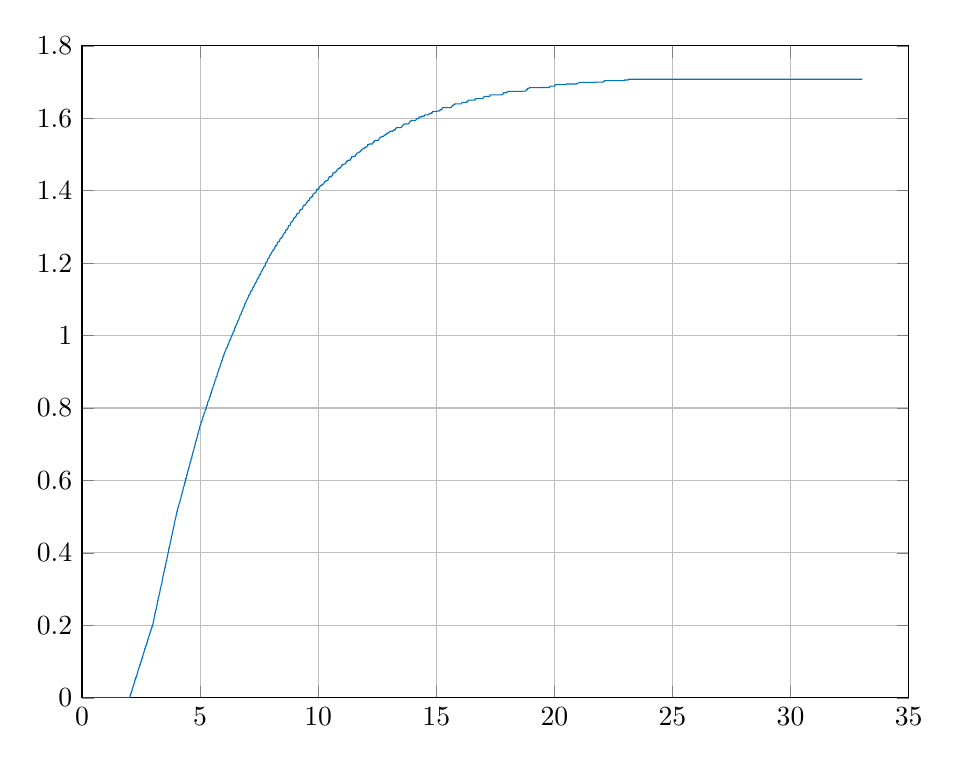
\begin{tikzpicture}

\begin{axis}[%
width=4.133in,
height=3.26in,
at={(0.693in,0.44in)},
scale only axis,
xmin=0,
xmax=35,
xmajorgrids,
ymin=0,
ymax=1.8,
ymajorgrids,
axis background/.style={fill=white}
]
\addplot [color=mycolor1,solid,forget plot]
  table[row sep=crcr]{%
0	0\\
0.0174364199999999	0\\
0.0324413389999997	0\\
0.0480745519989999	0\\
0.0640998179989997	0\\
0.0802082269989997	0\\
0.0962292989999996	0\\
0.112140156998999	0\\
0.128197941	0\\
0.144129229999999	0\\
0.160211415	0\\
0.176086827998999	0\\
0.192200153	0\\
0.208225839	0\\
0.224227045999	0\\
0.240080554	0\\
0.256212316	0\\
0.272087498	0\\
0.287968980998999	0\\
0.304175280999999	0\\
0.320220736	0\\
0.336536562	0\\
0.352217476999	0\\
0.368193181	0\\
0.384155161001	0\\
0.400024181	0\\
0.415951047999999	0\\
0.431919778999	0\\
0.447973876999999	0\\
0.464059460999	0\\
0.480058576	0\\
0.496060176999	0\\
0.512173605	0\\
0.528068001999999	0\\
0.544010151	0\\
0.559998673	0\\
0.576011581999999	0\\
0.591989840999001	0\\
0.608012696998999	0\\
0.624180601999001	0\\
0.640136015	0\\
0.655922871	0\\
0.674092178999	0\\
0.689323626999999	0\\
0.704526350000001	0\\
0.720011259000001	0\\
0.736073612999999	0\\
0.752035972	0\\
0.768029434998999	0\\
0.784062675	0\\
0.799996894999	0\\
0.816036227998999	0\\
0.832063142999	0\\
0.848087181999999	0\\
0.864017762999999	0\\
0.880263498999	0\\
0.896149981	0\\
0.911956988998999	0\\
0.928179579998999	0\\
0.944204442999999	0\\
0.960016884999	0\\
0.976101866998999	0\\
0.992018666999	0\\
1.010025436999	0\\
1.025319382	0\\
1.040847788	0\\
1.056282832	0\\
1.072203170999	0\\
1.088214014	0\\
1.10410021	0\\
1.120184143999	0\\
1.136192742999	0\\
1.153332650999	0\\
1.169049851999	0\\
1.184664222999	0\\
1.200207943999	0\\
1.216198867	0\\
1.232058714	0\\
1.248018682	0\\
1.264163278999	0\\
1.280203778999	0\\
1.296205294999	0\\
1.312056418999	0\\
1.328273238999	0\\
1.34413268	0\\
1.36020774	0\\
1.376078550999	0\\
1.392107234999	0\\
1.408105734	0\\
1.424191177	0\\
1.439961965999	0\\
1.455935304	0\\
1.47206816	0\\
1.488172840999	0\\
1.504562021999	0\\
1.520175550999	0\\
1.536107556	0\\
1.552158274999	0\\
1.568218684999	0\\
1.584080896999	0\\
1.600417683999	0\\
1.616165892999	0\\
1.632020097999	0\\
1.64800708	0\\
1.663921684	0\\
1.679974225	0\\
1.696183247	0\\
1.712205491999	0\\
1.728202698	0\\
1.74413995	0\\
1.760297773	0\\
1.776070962999	0\\
1.792014729999	0\\
1.808010689999	0\\
1.824178137999	0\\
1.840175485999	0\\
1.856258517999	0\\
1.872046412	0\\
1.888057365999	0\\
1.903962273	0\\
1.920177224999	0\\
1.936126995999	0\\
1.952091072999	0\\
1.968175580999	0\\
1.984195162	0\\
2.000203769999	0\\
2.017723236	0\\
2.03286175	0.00586034118541264\\
2.047944468	0.00586034118541264\\
2.063966206	0.0117206823708253\\
2.079946495999	0.0125895031546256\\
2.098116071999	0.0188677161208431\\
2.113148563999	0.0188677161208431\\
2.128386502	0.0247280573062557\\
2.144113648	0.0286325398120069\\
2.159934625999	0.0305883984916684\\
2.17611003	0.0344928809974196\\
2.19209383	0.036448739677081\\
2.208082964	0.0403532221828322\\
2.224121148999	0.043177901646294\\
2.240056938	0.0494561146125115\\
2.256037618	0.0494561146125115\\
2.274214714	0.0553164557979241\\
2.289394059	0.0553164557979241\\
2.30458258	0.0611767969833368\\
2.320164677999	0.0611767969833368\\
2.337081984	0.0670371381687494\\
2.35244274	0.0679059589525498\\
2.368217484	0.0741841719187672\\
2.384157628001	0.0780886544245184\\
2.400174926	0.0800445131041799\\
2.416436913	0.0839489956099311\\
2.432192117999	0.0859048542895925\\
2.448213056	0.0917651954750052\\
2.463979465	0.0917651954750052\\
2.480214109999	0.0980662505861902\\
2.496150904	0.0984943574442182\\
2.51202091	0.104772570410436\\
2.528092401	0.104772570410436\\
2.544057696	0.110632911595848\\
2.560052073	0.110632911595848\\
2.576022575	0.116493252781261\\
2.592061983	0.120397735287012\\
2.608066929	0.122794307892446\\
2.624044757	0.127126897256225\\
2.640132328999	0.129082755935887\\
2.656117033999	0.135360968902104\\
2.67206056	0.135360968902104\\
2.688063049	0.141221310087517\\
2.704059540999	0.141221310087517\\
2.720050849	0.147081651272929\\
2.736020509999	0.147522365198702\\
2.752026533	0.153382706384114\\
2.768011547999	0.153810813242142\\
2.784059405999	0.16008902620836\\
2.800047727999	0.162042670116064\\
2.816122816999	0.165949367393772\\
2.832212373999	0.169853849899524\\
2.848164019	0.171809708579185\\
2.864079035	0.177670049764598\\
2.880064906999	0.17811076369037\\
2.895952181999	0.184399211733811\\
2.912846776	0.184399211733811\\
2.928184557999	0.190677424700028\\
2.944053722999	0.190677424700028\\
2.960053562	0.196537765885441\\
2.975999719	0.196537765885441\\
2.994254925999	0.202398107070853\\
3.008585559999	0.20479246490433\\
3.024117377	0.212579908283799\\
3.040093882999	0.213008015141827\\
3.056201951999	0.222749102429\\
3.072171406	0.224136351638374\\
3.088090247	0.233877438925547\\
3.104069609	0.233877438925547\\
3.120078504	0.241662667533059\\
3.136031345001	0.243618526212721\\
3.151960363999	0.247499272314481\\
3.168030761999	0.255742011688902\\
3.184088748	0.258650450955996\\
3.200043123999	0.268391538243169\\
3.216096242999	0.268819645101197\\
3.232345321	0.276604873708709\\
3.248246571	0.278978604169175\\
3.264068767999	0.282859350270936\\
3.280051673	0.288719691456349\\
3.296060010999	0.292600437558109\\
3.312053810999	0.299430156172091\\
3.328149971999	0.303751616199624\\
3.344134951999	0.307656098705375\\
3.359977662999	0.313492703486797\\
3.378183431	0.313920810344825\\
3.393311515	0.323661897631999\\
3.408329681	0.325603581895234\\
3.423965118999	0.334310794641327\\
3.440091207998	0.338670980230306\\
3.456068635999	0.342575462736058\\
3.472002359999	0.34841206751748\\
3.488001425	0.350365711425184\\
3.50399475	0.358593868730425\\
3.520059731999	0.358593868730425\\
3.536060682999	0.368334956017599\\
3.552030617999	0.369732440304196\\
3.568062920999	0.379473527591369\\
3.584051137999	0.379473527591369\\
3.600061967	0.385725789381638\\
3.616100809	0.391574170922582\\
3.632072217999	0.395466876668812\\
3.648039532	0.401315258209755\\
3.664712465999	0.404184971915404\\
3.680096951	0.414405498689796\\
3.695980576999	0.414405498689796\\
3.712197562	0.420667995557288\\
3.728204576999	0.424574692834997\\
3.744034690999	0.430409082844461\\
3.760202780999	0.43431578012217\\
3.776177844	0.439104335946086\\
3.792106691	0.445444116618717\\
3.808257335999	0.449324862720478\\
3.824203394	0.453670059152002\\
3.840289837999	0.459506663933424\\
3.856198254999	0.463401992104363\\
3.872320295	0.469247751220597\\
3.888010259	0.47161754234186\\
3.903925231999	0.479906883307148\\
3.920045058999	0.484267068896128\\
3.936110399	0.488171551401879\\
3.952102193	0.494426027964106\\
3.967993017	0.49637967187181\\
3.984011323	0.504607829177051\\
4.000032677999	0.504607829177051\\
4.017330059	0.514838854405575\\
4.032641609	0.514838854405575\\
4.048226707	0.521152683902259\\
4.064199278999	0.525487488037995\\
4.080152432999	0.52742917230123\\
4.096619945999	0.53132187804746\\
4.112303497	0.535228575325168\\
4.128193923	0.539109321426929\\
4.144085671	0.541480837115438\\
4.159940774	0.547329218656382\\
4.177991844	0.549758218436257\\
4.192873846999	0.552632015756953\\
4.208390108	0.560419459136422\\
4.224197497	0.560419459136422\\
4.240197639999	0.566253849145887\\
4.256212827999	0.570160546423595\\
4.272338436999	0.572530337544858\\
4.288223765999	0.580329740568796\\
4.304298875	0.582271424832032\\
4.320226073999	0.584700424611907\\
4.338806023	0.59056076579732\\
4.35426679	0.595338823167104\\
4.369876093999	0.595338823167104\\
4.385399932999	0.605079910454277\\
4.4010598	0.60552062438005\\
4.416364753001	0.60552062438005\\
4.432178811	0.615261711667223\\
4.448292142	0.615261711667223\\
4.464212710999	0.621586039618038\\
4.480030828	0.625920843753775\\
4.496202891	0.628341967504229\\
4.512198484999	0.632234673250458\\
4.528154323999	0.636141370528167\\
4.544188686	0.640022116629927\\
4.560194137999	0.641975760537631\\
4.576274293	0.650181075697905\\
4.592259242999	0.650181075697905\\
4.608199813	0.654517117794617\\
4.624300734999	0.660852814852201\\
4.64027266	0.660852814852201\\
4.656180592	0.667166644348885\\
4.672191971	0.671073341626593\\
4.688079760999	0.675382194586382\\
4.704200662999	0.679291697173747\\
4.720204184	0.68318422003503\\
4.736184309999	0.685123281873555\\
4.752069476999	0.690974468724156\\
4.768200349	0.695354307102079\\
4.784186788999	0.695772178882884\\
4.800115549998	0.706433419583048\\
4.816082899999	0.706433419583048\\
4.832065785	0.708375103846283\\
4.848044270999	0.716174506870221\\
4.864202106999	0.716174506870221\\
4.880229006999	0.720055252971982\\
4.896204436	0.725915594157395\\
4.912107910999	0.730714385058533\\
4.928169884999	0.730714385058533\\
4.944215616999	0.738516410507181\\
4.960190734	0.740934911832925\\
4.976067642	0.74288855574063\\
4.992011913999	0.750675999120099\\
5.009937497	0.751534584826676\\
5.024994391998	0.753476269089911\\
5.040080075	0.76127580987677\\
5.056301701	0.76127580987677\\
5.072096184999	0.76370709364376\\
5.088119672	0.767599765775899\\
5.1041215	0.771506463053607\\
5.12031192	0.775387380057834\\
5.136008354999	0.776294888769898\\
5.152018478999	0.780204391357264\\
5.168155486999	0.786036232322164\\
5.184126971999	0.786036276032512\\
5.200222323	0.787989919940216\\
5.216202545999	0.795777704888328\\
5.232202991999	0.795777704888328\\
5.248138389	0.795777829824052\\
5.264081293999	0.804497464856404\\
5.280199671	0.806866175235256\\
5.296137108	0.806866042766132\\
5.312170363	0.811226740353621\\
5.328191163999	0.817087081539033\\
5.344200639999	0.819028714307328\\
5.360208571999	0.820968373270673\\
5.37619716	0.822922017178377\\
5.392456622	0.828770428080397\\
5.409543821999	0.831138278968995\\
5.425040842999	0.831138278968995\\
5.440446882	0.837476467385467\\
5.456213241	0.84136713502222\\
5.472084109	0.84136713502222\\
5.488205918	0.845262315340288\\
5.504746311	0.851588366092968\\
5.520214770999	0.85202908001874\\
5.536072732	0.854388636062781\\
5.552104776	0.860238070161629\\
5.568203873	0.862188908759677\\
5.584268137999	0.864130593022912\\
5.600219861999	0.868024333641419\\
5.616093009	0.871931030919128\\
5.63218009	0.876298674599074\\
5.648047674	0.876298514007458\\
5.663950050999	0.87868026477319\\
5.680101163999	0.886468814794456\\
5.696208217	0.886948173748234\\
5.712189446999	0.886948173748234\\
5.728124238	0.894739613791815\\
5.744016382999	0.896690451796394\\
5.759969333	0.898632136059629\\
5.776390062	0.90296683173964\\
5.792203684	0.906873608245644\\
5.808111793	0.909299813664793\\
5.824230427999	0.911658107886581\\
5.840264067999	0.913611572051144\\
5.85619913	0.919459953592088\\
5.872219665999	0.921400460568411\\
5.888061250999	0.923833543963334\\
5.904005122	0.927730986733662\\
5.920174464999	0.931622416784261\\
5.936176504	0.932050523642289\\
5.952099142	0.935945831093011\\
5.968218316999	0.941793204240386\\
5.984208788999	0.941793204240386\\
6.000112769999	0.944218113485054\\
6.017582649	0.950068376300085\\
6.032675724	0.952459928823904\\
6.04809412	0.954401577097694\\
6.064063339999	0.95634242162424\\
6.080053071	0.958775166124028\\
6.096028728999	0.962681562384189\\
6.112248274999	0.965041285665884\\
6.128208428999	0.966982214432187\\
6.14396666	0.966982171575678\\
6.159953748999	0.968935714601241\\
6.176064281	0.97478434690994\\
6.192075689999	0.976725359856877\\
6.208060142999	0.976725373160571\\
6.224060497999	0.981102846913868\\
6.240172138999	0.987378748118049\\
6.256208938	0.987378579434832\\
6.272330718	0.987378579434832\\
6.288081672	0.989320681348556\\
6.30405878	0.993215494258392\\
6.320175488	0.997599597433803\\
6.336359641	0.997599597433803\\
6.352202451999	1.0019235669667\\
6.368325165	1.0038772108744\\
6.384229085999	1.00583306955406\\
6.399927596999	1.00972605410046\\
6.418094974999	1.01166748706362\\
6.433175913	1.01166748706362\\
6.448245408999	1.01403900852313\\
6.464020657999	1.02036820233548\\
6.480112335999	1.02230971912447\\
6.496167585	1.02230946421086\\
6.512213201999	1.0262056480661\\
6.528219730999	1.03010310730144\\
6.544099521999	1.03205394589949\\
6.560153358	1.03252957914858\\
6.576187239	1.03490028714862\\
6.591977611	1.03879561531956\\
6.608326035999	1.0427020511755\\
6.624058384	1.0427020511755\\
6.640218780999	1.04464473531513\\
6.655994672	1.04854004068558\\
6.672041295999	1.05049589936524\\
6.688202523	1.05483021896712\\
6.704048743999	1.05725054151337\\
6.720080634999	1.05725054151337\\
6.736160679	1.05920418542107\\
6.752048283	1.06505351303313\\
6.768064769999	1.06699553153507\\
6.784071057999	1.06741340331587\\
6.800020132	1.06984119099318\\
6.816298351	1.07373978878465\\
6.832204156999	1.07763272929642\\
6.848177184999	1.07763272929642\\
6.864213294999	1.07957549446255\\
6.880201443	1.0834713236366\\
6.896166096999	1.08780612777234\\
6.911979625999	1.08780594857729\\
6.92806041	1.0897491294598\\
6.944051668999	1.09412210884248\\
6.960060702999	1.09607760297213\\
6.976001891	1.09802844157018\\
6.992188637	1.09997170503601\\
7.009917887999	1.10235455959676\\
7.025062535	1.10430820350447\\
7.040364753001	1.10673672100751\\
7.056003098	1.11063042528951\\
7.072091451999	1.11257294337473\\
7.088046931	1.11257294337473\\
7.104099507999	1.11257277303856\\
7.120061782	1.1164696883935\\
7.136064551999	1.12231898681322\\
7.151995634999	1.1227367649757\\
7.170209929999	1.12273660162915\\
7.185489417	1.12273660162915\\
7.200828347999	1.12663383874399\\
7.21612082	1.12905145118171\\
7.232095876999	1.13295814845942\\
7.248067061	1.13295814845942\\
7.264062109	1.13490144988472\\
7.280057412	1.13532955674275\\
7.296058128001	1.13922605060778\\
7.312066129999	1.14118160516847\\
7.328052112	1.14313244376652\\
7.344019281	1.14554690715542\\
7.359993398999	1.14748934848413\\
7.376050155	1.14748934848413\\
7.392077826999	1.14944299239183\\
7.407967070999	1.15378306453842\\
7.424091946999	1.15573390313646\\
7.440058199	1.15767700137646\\
7.456025599	1.15767686115272\\
7.472217814	1.15963029234568\\
7.488063783999	1.16157437838856\\
7.504063803	1.16742425654878\\
7.520128848999	1.16789705293952\\
7.536059997	1.16789705293952\\
7.552213804999	1.16789705293952\\
7.568210811999	1.17221226440323\\
7.584116689999	1.17611146907284\\
7.600213226	1.17806230767089\\
7.616205160999	1.17806190456389\\
7.632079521	1.1804748238806\\
7.647950417	1.18241825233548\\
7.666106786001	1.18437130450787\\
7.681468854999	1.18632716318753\\
7.696943389	1.1887061086436\\
7.712615464	1.19064999845503\\
7.728273618999	1.19259359166217\\
7.744215101	1.19259359166217\\
7.760236634	1.19454704572659\\
7.776114829999	1.20039805465407\\
7.792352809999	1.20234173014853\\
7.808138939999	1.20325329237218\\
7.824086795999	1.20325310201072\\
7.840110754	1.20520674591842\\
7.856078049	1.20910726292145\\
7.872126637999	1.21300136505268\\
7.888043507999	1.21300136505268\\
7.903946002	1.21300136505268\\
7.920086553999	1.2149456782286\\
7.936316118	1.21930979543693\\
7.952195795	1.22126565411659\\
7.968162714	1.22321579466486\\
7.984209183	1.22321579466486\\
8.000211878001	1.22557856914359\\
8.016028740999	1.22752233781078\\
8.032065369	1.22947598171849\\
8.048202825	1.23143184039815\\
8.064173947999	1.23338243651933\\
8.080183639	1.23532733921725\\
8.096363681	1.23532733921725\\
8.11214023	1.2372713394957\\
8.128158209	1.2372713394957\\
8.144422215999	1.24012201725957\\
8.160094943999	1.24207787593923\\
8.176183418	1.24597310304433\\
8.192197979999	1.24791743470566\\
8.208134901999	1.24791743470566\\
8.224202899999	1.24791699510325\\
8.240206561999	1.24791699510325\\
8.256082894999	1.25225625563464\\
8.272055693	1.25421166748677\\
8.288083318999	1.25810700119563\\
8.304080361999	1.25857321305265\\
8.320199710999	1.2585728406359\\
8.336408568	1.2585728406359\\
8.352774370999	1.26051774333382\\
8.368230387	1.26247100754045\\
8.384177747	1.26637152454349\\
8.400262842	1.26832236314153\\
8.416117839999	1.26832205767357\\
8.431974916	1.26832205767357\\
8.448092601999	1.27026696037149\\
8.464086698	1.27026664755998\\
8.480081342999	1.27416511276666\\
8.496115599999	1.27416511276666\\
8.512198596999	1.27807181004437\\
8.528179257	1.280900557624\\
8.544071862999	1.280900557624\\
8.560199276	1.28284546032192\\
8.576202712	1.28284495604608\\
8.592157599999	1.28479859995379\\
8.608204613999	1.28479859995379\\
8.624250753001	1.29064968817738\\
8.640201991999	1.29064968817738\\
8.655952028	1.29302286035347\\
8.674264316	1.29302242234644\\
8.690029313	1.29348863420345\\
8.70533116	1.29544227811116\\
8.720462252	1.29738673526662\\
8.736054311	1.30129343254433\\
8.752167026	1.30367937417131\\
8.768216337	1.30367900219614\\
8.784117234999	1.30367900219614\\
8.800222247999	1.30367900219614\\
8.816085878001	1.30562390489406\\
8.832200255999	1.30952255907927\\
8.848208899999	1.31342925635698\\
8.864074028	1.31342925635698\\
8.879972388999	1.31342895017668\\
8.898176418999	1.31583768823736\\
8.913392229999	1.31583768823736\\
8.92820018	1.31778258660381\\
8.944193965	1.31973623051152\\
8.960134269	1.32364292778923\\
8.976188917	1.3236423475969\\
8.99227928	1.32558725029482\\
9.010184870999	1.32558725029482\\
9.02539478	1.3275327368982\\
9.040911420999	1.3275327368982\\
9.056161129	1.32990459394208\\
9.072005068999	1.33037099284265\\
9.088078109	1.33427754413643\\
9.104068896999	1.33622244683435\\
9.120023436	1.33622255250343\\
9.136077655	1.3381681851255\\
9.151989933	1.3381681851255\\
9.168026231	1.3381681851255\\
9.184192672	1.33816828244186\\
9.200145398999	1.34012192634956\\
9.216075017999	1.344022395521\\
9.232121800999	1.34640135674024\\
9.248089691999	1.34834698936231\\
9.264096814999	1.34834698936231\\
9.280090168	1.34834699671318\\
9.295993071999	1.34834699671318\\
9.314136978	1.34878771063895\\
9.329233987	1.35073261227545\\
9.344568609999	1.35268625618315\\
9.360134695	1.35705039173573\\
9.376179540999	1.35900114748089\\
9.392306382	1.35900114748089\\
9.407975764	1.35900114748089\\
9.424032971	1.35900105615615\\
9.440175618	1.36094595885407\\
9.456204844	1.36094595885407\\
9.47216182	1.36289159147614\\
9.488058073999	1.36484513558725\\
9.504047424	1.3668002619645\\
9.520006595001	1.36875110056254\\
9.536055745999	1.36875091873626\\
9.552117752999	1.3711620332912\\
9.568094486	1.3711620332912\\
9.584199884999	1.37310747555558\\
9.600003557	1.37310747555558\\
9.615998725	1.37310747555558\\
9.632118151999	1.37701582609927\\
9.648181718999	1.37896666469732\\
9.6641735	1.38091156739524\\
9.680241717999	1.38091128623828\\
9.696210542	1.38091128623828\\
9.712220362999	1.38327956845325\\
9.728217976	1.38327961988143\\
9.744161601999	1.38327961988143\\
9.760112507	1.38327961988143\\
9.776056043999	1.38913289344836\\
9.792012257	1.39108373204641\\
9.807986535	1.39108373204641\\
9.824083686	1.39302936466848\\
9.840049543	1.393492481211\\
9.856053837	1.393492481211\\
9.87206002	1.393492481211\\
9.888050457	1.3939205397111\\
9.903937345001	1.39586544240903\\
9.922163447	1.40021433648964\\
9.937634653	1.40411067665427\\
9.953129364	1.40411067665427\\
9.968507009	1.40411067665427\\
9.984406637999	1.40411053687591\\
10.000217073	1.40411053687591\\
10.017969955	1.40605543957383\\
10.033488119999	1.4065215029296\\
10.048571818	1.40846713555166\\
10.064066002	1.41042144951756\\
10.080080618999	1.41237486198833\\
10.096186568	1.41432570058638\\
10.112210625999	1.41432570058638\\
10.128145726	1.41432546036705\\
10.144204910999	1.41432546036705\\
10.159938590999	1.41627036306497\\
10.176176891	1.41627036306497\\
10.192216039	1.41821574668531\\
10.208161094	1.41821574668531\\
10.224046457	1.41821574668531\\
10.240191195	1.42016950565868\\
10.25609008	1.42212314956639\\
10.272064229999	1.42407398816443\\
10.288082545999	1.42601854984495\\
10.304050887999	1.42601854984495\\
10.319991915999	1.42601854984495\\
10.336056162999	1.42796383260773\\
10.352059774999	1.42796383260773\\
10.368178226999	1.42796383260773\\
10.384231177	1.42842663014365\\
10.400195154	1.42842663014365\\
10.416024529	1.43038042336981\\
10.432109223999	1.43275264977155\\
10.448068096	1.4366571322773\\
10.464246115	1.4366571322773\\
10.480207807999	1.43860276489936\\
10.496232162	1.43860265480719\\
10.512324549998	1.43860265480719\\
10.528215467	1.43860265480719\\
10.544222823	1.43860253580062\\
10.560126141	1.43860253580062\\
10.576121762	1.44054743849854\\
10.592047838	1.44250080492878\\
10.608060882	1.44250080492878\\
10.624047891998	1.44881713191361\\
10.640089960999	1.44881692021074\\
10.656113156999	1.44881692021074\\
10.672093887999	1.44924502706877\\
10.688308031999	1.44968552031778\\
10.704151377	1.44968552031778\\
10.720198939	1.45163042301571\\
10.736174438	1.45163019336507\\
10.752210641	1.45163019336507\\
10.768198273	1.45357582598713\\
10.784261927	1.45552878188674\\
10.800130243999	1.45748242579445\\
10.816293451	1.45943326439249\\
10.832309474	1.45943326439249\\
10.848255181	1.45943294168859\\
10.864332035999	1.46137784438651\\
10.880404217999	1.46137784438651\\
10.896335146999	1.46137751264925\\
10.911954291	1.46332314527132\\
10.92818571	1.46332314527132\\
10.943977613999	1.46332280450071\\
10.960189547999	1.4652757735298\\
10.976184509999	1.4672294174375\\
10.992134073999	1.4696429871847\\
11.008082330999	1.47158773591378\\
11.024231929	1.47158708256024\\
11.040197245	1.47158708256024\\
11.056075523	1.47158708383712\\
11.072125294999	1.47353205318118\\
11.088084674	1.47353205318118\\
11.104015208999	1.47353204533885\\
11.120054285999	1.47353128368611\\
11.136115278	1.47353128368611\\
11.152140017	1.47548416046966\\
11.167985531999	1.47548398016932\\
11.184181004	1.4793822528575\\
11.200179856	1.48133275722305\\
11.216176351999	1.48133264924825\\
11.23215628	1.48133204153635\\
11.248217498	1.48327796521114\\
11.26421231	1.48374202330436\\
11.280067560999	1.48374148731133\\
11.296085229999	1.48417300326744\\
11.312042231999	1.48417241651313\\
11.328179461999	1.48417187166969\\
11.3446142	1.48417187166969\\
11.360203604	1.48611721175752\\
11.376146488	1.48806915869393\\
11.392205656999	1.48806915869393\\
11.407981149	1.49002266267933\\
11.423929568999	1.49391827719995\\
11.440186409	1.49391827719995\\
11.456194918999	1.49391805067492\\
11.472014035	1.49391763974052\\
11.488117798	1.49391714861884\\
11.504316311999	1.49391691285579\\
11.520250436	1.49391649301164\\
11.536185748	1.49391599298033\\
11.552139262	1.49586154215484\\
11.568174371	1.49586119408879\\
11.584267846	1.49628879200589\\
11.600248576999	1.50063274258975\\
11.616204946999	1.50063247164615\\
11.63221312	1.50258567779832\\
11.648209941	1.50453558908929\\
11.663996004	1.50453522226343\\
11.680128519999	1.50453477553901\\
11.696163823999	1.50453477553901\\
11.712303564999	1.50453476540627\\
11.728084547	1.50693811231261\\
11.744057790999	1.50693811231261\\
11.760244778	1.50693809286893\\
11.776229196999	1.50888390333151\\
11.792264014999	1.50888390333151\\
11.808331186	1.51083676832199\\
11.825191298	1.51083572222094\\
11.840621656999	1.51278936612864\\
11.856223063	1.51473885045148\\
11.872230283999	1.51473852890374\\
11.888200314999	1.51473778628014\\
11.904167559999	1.51668401869053\\
11.920138774	1.51668376838743\\
11.936170007999	1.51668301672179\\
11.952202912	1.51863003982206\\
11.968161111	1.51862978043146\\
11.984070997	1.51862909940363\\
12.000056677999	1.51862909940363\\
12.017315042	1.52104126911227\\
12.032281806	1.52104126911227\\
12.048081410999	1.52104126911227\\
12.064308474	1.52104126911227\\
12.080278104	1.52299491301998\\
12.096073921	1.52689071958615\\
12.112073715	1.52689071958615\\
12.128202931	1.52689071958615\\
12.144180404	1.52689071958615\\
12.160081519	1.52883795707173\\
12.176206906999	1.52883795707173\\
12.192068107	1.52883795707173\\
12.208199363	1.52883795707173\\
12.22407479	1.52883795707173\\
12.240057064	1.52883795707173\\
12.256054823	1.52883795707173\\
12.2720362	1.52883795707173\\
12.288030491	1.52883795707173\\
12.304027457998	1.53079085081682\\
12.320016186999	1.5327373690488\\
12.336050924	1.5327373690488\\
12.352062083	1.53512252891262\\
12.368033031999	1.53512252891262\\
12.384199802999	1.53901905473238\\
12.400176484999	1.53901905473238\\
12.415988171999	1.53901905473238\\
12.432075977999	1.53901905473238\\
12.448216396999	1.53901905473238\\
12.464242686	1.53901905473238\\
12.480121139	1.53901905473238\\
12.496033755	1.53901905473238\\
12.512193856999	1.53901905473238\\
12.528225082	1.53901905473238\\
12.544176526	1.53901905473238\\
12.560273396	1.54096557296437\\
12.576195802999	1.54291846670946\\
12.592181449	1.54486570419504\\
12.608272439999	1.54532206608516\\
12.624093889	1.54727570999287\\
12.640066861999	1.54727570999287\\
12.6559628	1.54727570999287\\
12.672079446999	1.54922499832705\\
12.688097774	1.54922499832705\\
12.704333130999	1.54967251926535\\
12.720306903	1.54967251926535\\
12.736221915	1.55010062612338\\
12.752089722999	1.55010062612338\\
12.768073213	1.55010062612338\\
12.783995431	1.55204714435537\\
12.800007804999	1.55204714435537\\
12.816050023	1.55399438184095\\
12.83209339	1.55399438184095\\
12.848042714	1.55399438184095\\
12.864146927	1.55594727558604\\
12.880118554	1.55594727558604\\
12.896110917	1.55790091949374\\
12.91206448	1.55790091949374\\
12.928080915999	1.55790091949374\\
12.944202627	1.55790091949374\\
12.960184784	1.55985020782792\\
12.976024661001	1.55985020782792\\
12.992227343999	1.56030962786726\\
13.010088955	1.56225614609925\\
13.025480401	1.56225614609925\\
13.040947026	1.5642031099975\\
13.056400221999	1.5642031099975\\
13.072421052999	1.5642031099975\\
13.088182045999	1.5642031820553\\
13.104083917	1.56420281720703\\
13.120068872	1.56420281720703\\
13.13606193	1.56420287965668\\
13.152128434999	1.56420250521341\\
13.168114924	1.56615517274959\\
13.184053543	1.56615517274959\\
13.200015246	1.56615476603091\\
13.216070555	1.56810811058758\\
13.232188236	1.56810811058758\\
13.248141116999	1.56810760961977\\
13.26421102	1.56810760961977\\
13.280210879	1.57200341618594\\
13.296234049998	1.57200289589605\\
13.312201075	1.57395013338163\\
13.328236222999	1.57395013338163\\
13.344222486	1.57394959376967\\
13.360206333999	1.57394959376967\\
13.376192356	1.57394959376967\\
13.392119818999	1.57394903483566\\
13.407962903999	1.57394903483566\\
13.426396255999	1.57394903483566\\
13.441892443	1.57394896441188\\
13.457407142999	1.57394845657961\\
13.472815811999	1.57394845657961\\
13.488056892999	1.57394837648818\\
13.504058335	1.57394785900154\\
13.520110141	1.57589999663516\\
13.536202068	1.57589999663516\\
13.552206391998	1.57785212219845\\
13.568088538999	1.57979864043044\\
13.584002033999	1.57979864043044\\
13.600041446	1.58174509029328\\
13.616008505	1.58369437862747\\
13.631974613999	1.58369437862747\\
13.648012806	1.58369357156382\\
13.663901446999	1.58369357156382\\
13.680061205	1.58414993345394\\
13.69632314	1.58414910694942\\
13.712179460999	1.58414910694942\\
13.728084750999	1.58414910694942\\
13.743986149999	1.58414890293837\\
13.760055311999	1.58458488813939\\
13.776062998999	1.58458488813939\\
13.792184378001	1.58458467440124\\
13.808313684999	1.58458436339244\\
13.824265479999	1.58458436339244\\
13.840226965999	1.58653088162443\\
13.856213990999	1.58653033742336\\
13.872097174998	1.58847757490894\\
13.888206016	1.59238154481777\\
13.904039655	1.59238082904832\\
13.919964221	1.59238082904832\\
13.936103005	1.59238082904832\\
13.952180613999	1.59238009370587\\
13.968192709	1.59432938204005\\
13.984070132	1.59432938204005\\
14.000051488999	1.59432862712463\\
14.016011151999	1.59432862712463\\
14.034246443999	1.59432789423161\\
14.049343563	1.59432789423161\\
14.064405297	1.59432789423161\\
14.080171981999	1.59432715173497\\
14.096061645999	1.59432715173497\\
14.112229215	1.59432715173497\\
14.128208261	1.59432639963474\\
14.144170935999	1.59627291786672\\
14.160048948999	1.59672043880503\\
14.17606949	1.59866723271294\\
14.192172597	1.59866723271294\\
14.208240257	1.59912665275227\\
14.224071500999	1.59912665275227\\
14.240099358	1.59956088456786\\
14.256054384999	1.59956088456786\\
14.27218038	1.6034643977771\\
14.288206633	1.60346369619009\\
14.304213702999	1.60346369619009\\
14.320425275999	1.60346369619009\\
14.33652227	1.60346298494025\\
14.352191584999	1.60346298494025\\
14.368370188	1.60346298494025\\
14.384222978999	1.60541155236178\\
14.400103646999	1.60541155236178\\
14.416020157999	1.60541155236178\\
14.431916567	1.60541082178633\\
14.448193839	1.60541082178633\\
14.464190675999	1.60541082178633\\
14.480051981	1.6054100815481\\
14.496002953999	1.60735659978009\\
14.512052755999	1.60930463080121\\
14.528050965999	1.60930463080121\\
14.544508546	1.60930395992746\\
14.560222451999	1.60930395992746\\
14.576060674998	1.60930395992746\\
14.592227091	1.60930327933164\\
14.6082781	1.60930327933164\\
14.624190004999	1.60930327933164\\
14.640100294999	1.60930258901377\\
14.655963758	1.60930258901377\\
14.67435481	1.60930258901377\\
14.689904813	1.61125326454948\\
14.705240781999	1.61320540218311\\
14.720675092999	1.61320540218311\\
14.7361544	1.6132046924212\\
14.752174096	1.6132046924212\\
14.768177503001	1.6132046924212\\
14.784122136999	1.61320397293731\\
14.800116461	1.6151532612715\\
14.816190267999	1.6151532612715\\
14.83196707	1.61515253206565\\
14.847890165	1.61904763326302\\
14.866124297	1.61904763326302\\
14.881334130999	1.619046972947\\
14.896480326	1.619046972947\\
14.911933860999	1.619046972947\\
14.928071076999	1.619046972947\\
14.944316551999	1.6190463028497\\
14.960207469	1.6190463028497\\
14.9761995	1.6190463028497\\
14.992234368	1.61904562297114\\
15.008099286001	1.61904521697453\\
15.024100913	1.61904521697453\\
15.040066068999	1.61904452731474\\
15.056057943999	1.6194937491574\\
15.072058004	1.61949333337909\\
15.088056785	1.61949229378453\\
15.103969566	1.61949229378453\\
15.120139771999	1.62144324380014\\
15.136092712999	1.62144219441072\\
15.152243794999	1.62144219441072\\
15.168113941999	1.62339389670267\\
15.184102256999	1.62339389670267\\
15.200057688	1.62339283751841\\
15.216106825	1.62339239239506\\
15.232155876	1.62534152439621\\
15.248052339999	1.62728745202373\\
15.264006459	1.62923636531068\\
15.280059804999	1.62923636531068\\
15.296075844999	1.62923536467367\\
15.312006465	1.62923497978549\\
15.328084943999	1.62923497978549\\
15.344091292	1.62923396929437\\
15.360216309	1.62923396929437\\
15.376174509	1.62923357456526\\
15.392242703	1.62923255422005\\
15.408148096999	1.62923255422005\\
15.424129934999	1.62923214965001\\
15.440208695999	1.62923111945075\\
15.456158507999	1.62923111945075\\
15.472113941	1.6292307050398\\
15.488208599	1.62922966498651\\
15.504318838	1.62922966498651\\
15.520073346	1.62922924073467\\
15.53606457	1.62922924073467\\
15.552151961999	1.62922819082739\\
15.568169015	1.62922775673466\\
15.584234967	1.62922775673466\\
15.599992284999	1.62922669697342\\
15.616203329999	1.62922625303981\\
15.632208891	1.62922625303981\\
15.648360293999	1.63117501705388\\
15.663979619999	1.63312257266561\\
15.680206142	1.63507357384999\\
15.696039139999	1.63507257204266\\
15.712021123	1.63507257204266\\
15.728025839999	1.63702432538488\\
15.743955066999	1.63702331366429\\
15.759945672	1.63746164386277\\
15.775934901999	1.63941053800539\\
15.791938962999	1.63940951637156\\
15.808067960999	1.63940951637156\\
15.824084071999	1.63940911227985\\
15.840209351999	1.63986275486957\\
15.856185299	1.63986172332255\\
15.872097137999	1.63986096935585\\
15.888054205	1.63986096935585\\
15.904087638	1.63985992789566\\
15.92043274	1.63985916401504\\
15.93625657	1.63985916401504\\
15.951973564999	1.63985811264171\\
15.96808757	1.63985733884718\\
15.984078196	1.63985733884718\\
16.000076363	1.63985627756075\\
16.017419304999	1.63985627756075\\
16.032518945	1.63985549385233\\
16.048038115	1.63985509211729\\
16.064179457	1.63985509211729\\
16.080089608	1.64180467450892\\
16.096209745	1.64375294243368\\
16.112211828	1.64375253066111\\
16.128254844999	1.64375180597417\\
16.144377260999	1.64375180597417\\
16.160760855999	1.64375138416409\\
16.176029596999	1.64375064950399\\
16.192246071	1.64375064950399\\
16.208142510999	1.6437502176564\\
16.224105165	1.64374947302316\\
16.240195369	1.64374947302316\\
16.256334673	1.64374903113808\\
16.272221095001	1.64419579747003\\
16.288179379	1.64419579747003\\
16.304288576	1.6461462610349\\
16.320204278999	1.6461462610349\\
16.336513197	1.64809763408907\\
16.352202608	1.64809709523968\\
16.368166186	1.65004638357386\\
16.384195255	1.65004560902133\\
16.400215299	1.65004506007506\\
16.415930625999	1.65004506007506\\
16.434085879	1.65004427554949\\
16.449159906	1.65004427554949\\
16.464250705	1.65004371650636\\
16.480304991999	1.65004292200776\\
16.496220203999	1.65004292200776\\
16.512202151999	1.6500423528678\\
16.528101413	1.6500415483962\\
16.544149997	1.6500415483962\\
16.560065990999	1.65004096915941\\
16.576004956	1.65004015471483\\
16.592207549	1.65047507845456\\
16.608268257	1.65047448912096\\
16.624206891	1.65047366470344\\
16.640209846999	1.65047366470344\\
16.656037902999	1.65437257328812\\
16.672152906	1.65437257328812\\
16.688111431	1.65437181709388\\
16.703996625	1.65437120756672\\
16.720035247	1.65437120756672\\
16.736058547999	1.6543704413402\\
16.752113936999	1.6543704413402\\
16.768028186999	1.65436982171629\\
16.784013280999	1.65436904545751\\
16.800015794	1.65436904545751\\
16.816002217	1.65436841573688\\
16.834184498	1.65436762944587\\
16.849542337	1.65436762944587\\
16.86514662	1.65436698962852\\
16.880608941	1.65436619330531\\
16.896201738	1.65436619330531\\
16.911969179999	1.65436554339126\\
16.928140903	1.65436473703587\\
16.944346658	1.65436473703587\\
16.960062028	1.65436407702515\\
16.976220510999	1.65631621465878\\
16.992099214	1.65631539827123\\
17.010168516	1.65826401649804\\
17.025185532999	1.66021385012727\\
17.040385821	1.66021385012727\\
17.056119436	1.66021309220214\\
17.072188115999	1.66021309220214\\
17.088083208	1.66021309220214\\
17.104207006999	1.66021309220214\\
17.120221293	1.660212324121\\
17.136083530999	1.660212324121\\
17.15214324	1.660212324121\\
17.16807357	1.66021154588389\\
17.184080165	1.66021154588389\\
17.200181538999	1.66021154588389\\
17.216337696999	1.66021075749081\\
17.23219012	1.66021075749081\\
17.248209078	1.66021075749081\\
17.264244281999	1.66065271553895\\
17.280027134	1.66455276968046\\
17.296024139999	1.66455276968046\\
17.312150650999	1.66455196097554\\
17.328212055	1.66455196097554\\
17.344199089	1.66455196097554\\
17.360207116999	1.66455114211473\\
17.376113889999	1.66455114211473\\
17.392192833	1.66455114211473\\
17.408053314	1.66455114211473\\
17.424054240999	1.66455031309806\\
17.440178337	1.66455031309806\\
17.456210342999	1.66455031309806\\
17.472166632999	1.66454947392556\\
17.488195597999	1.66454947392556\\
17.504290026	1.66454947392556\\
17.520261318	1.66454862459725\\
17.536259675	1.66454862459725\\
17.552192686999	1.66454862459725\\
17.568225189999	1.66454776511315\\
17.584186826999	1.66454776511315\\
17.600209372	1.66454776511315\\
17.616128137	1.6645468954733\\
17.632078518	1.6645468954733\\
17.648137262	1.6645468954733\\
17.664111214	1.66454601567771\\
17.680090593	1.66454601567771\\
17.696108155	1.66454601567771\\
17.711989486999	1.66454601567771\\
17.727963122	1.66454512572642\\
17.744046546	1.66454512572642\\
17.760160955999	1.66454512572642\\
17.776186971	1.66454422561946\\
17.792073266998	1.66454422561946\\
17.808062762999	1.66649636325309\\
17.824009902	1.66649545299047\\
17.840177325	1.66844403595586\\
17.856101064999	1.67039332429004\\
17.87219813	1.67039232520067\\
17.888239929	1.67039232520067\\
17.90405463	1.67039232520067\\
17.920141925	1.67039131589636\\
17.93616883	1.67039131589636\\
17.952186323	1.67039131589636\\
17.968221021999	1.67039029637712\\
17.984175643	1.67039029637712\\
18.000254143999	1.67233997450471\\
18.018006172	1.67428932078452\\
18.033270458999	1.67428932078452\\
18.048769523999	1.67428932078452\\
18.064204693	1.67428932078452\\
18.080065582	1.67428932078452\\
18.096057217999	1.67428932078452\\
18.112165546999	1.67428932078452\\
18.128240976999	1.67428932078452\\
18.144070955999	1.67428932078452\\
18.160050484	1.67428932078452\\
18.176161663	1.67428932078452\\
18.192220056	1.67428932078452\\
18.208210718	1.67428932078452\\
18.224198965999	1.67428932078452\\
18.240155497999	1.67428932078452\\
18.256261616999	1.67428932078452\\
18.272199965	1.67428932078452\\
18.28810054	1.67428932078452\\
18.304180894999	1.67428932078452\\
18.32028266	1.67428932078452\\
18.336715047999	1.67428932078452\\
18.352196646999	1.67428932078452\\
18.368243302	1.67428932078452\\
18.384243356999	1.67428932078452\\
18.400204653	1.67428932078452\\
18.415964153	1.67428932078452\\
18.432162104999	1.67428932078452\\
18.448199002	1.67428932078452\\
18.464213693999	1.67428932078452\\
18.480082736999	1.67428932078452\\
18.496054085999	1.67428932078452\\
18.512329413999	1.67428932078452\\
18.528374281999	1.67428932078452\\
18.544215648	1.67428932078452\\
18.560206361999	1.67428932078452\\
18.576181063999	1.67428932078452\\
18.592086497999	1.67428932078452\\
18.60805443	1.67428932078452\\
18.624091668	1.67428932078452\\
18.640203531	1.67428932078452\\
18.656050675999	1.67473514047766\\
18.672143573	1.67473514047766\\
18.688015255999	1.67473514047766\\
18.704205168999	1.67473514047766\\
18.720114759999	1.67473514047766\\
18.736113400999	1.67473514047766\\
18.752017885999	1.67473514047766\\
18.767996063999	1.67473514047766\\
18.783992958	1.67473514047766\\
18.800055800999	1.67668727811129\\
18.815995602999	1.67863554603604\\
18.831979512999	1.67863554603604\\
18.848051613999	1.67863554603604\\
18.864171389	1.68253560017755\\
18.880198159	1.68253560017755\\
18.896161239	1.68253560017755\\
18.912122826	1.68253560017755\\
18.928195885999	1.68253560017755\\
18.944174464	1.68448488851173\\
18.960220578	1.68448488851173\\
18.976193236999	1.68448488851173\\
18.992206917	1.68448488851173\\
19.010058407	1.68448488851173\\
19.025172686999	1.68448488851173\\
19.040321964	1.68448292976221\\
19.056013415	1.68448292976221\\
19.072056095001	1.68448292976221\\
19.08806064	1.68448095056525\\
19.104058222999	1.68448095056525\\
19.120027964	1.68448095056525\\
19.136040485999	1.68447895092091\\
19.152011939999	1.68447895092091\\
19.167919712999	1.68447895092091\\
19.186086677999	1.68447693082924\\
19.201346267	1.68447693082924\\
19.216753681999	1.68447693082924\\
19.232188496	1.68447595656605\\
19.24821316	1.68447489029032\\
19.264364828	1.68447489029032\\
19.280249966999	1.68447390580339\\
19.296053866999	1.6844728293042\\
19.312014967	1.6844728293042\\
19.328176573	1.6844728293042\\
19.344573856999	1.68447074787095\\
19.360188983	1.68447074787095\\
19.376205495	1.68447074787095\\
19.392118578	1.68492058856814\\
19.408143178	1.68492058856814\\
19.424033804	1.68492058856814\\
19.439990017	1.68491846624081\\
19.455997538999	1.68491846624081\\
19.472021389999	1.68491846624081\\
19.488201016	1.68491744085923\\
19.503907015	1.68491632346654\\
19.520158104	1.68491632346654\\
19.536123292	1.68491528786137\\
19.552187738999	1.68491416024539\\
19.568071299	1.68491416024539\\
19.584064634	1.68491311441667\\
19.600047208	1.68491197657743\\
19.616171092999	1.68491197657743\\
19.632108923	1.68491197657743\\
19.648104924998	1.68490977246272\\
19.664014674	1.68490977246272\\
19.680080488	1.68490977246272\\
19.696193202999	1.68490754790134\\
19.712053205	1.68490754790134\\
19.7280757	1.68490754790134\\
19.744310193999	1.68490530289335\\
19.760209102999	1.68490530289335\\
19.776311360999	1.68490530289335\\
19.792258669999	1.68490303743882\\
19.808181299	1.68685395292624\\
19.8241227	1.68880555774351\\
19.840333762	1.68880453762745\\
19.856235088	1.68880342496744\\
19.872125064	1.68880342496744\\
19.888122551999	1.68880239456859\\
19.904304087	1.68880127162609\\
19.919991442	1.68880127162609\\
19.93586866	1.68880023094449\\
19.95188478	1.68879909771952\\
19.968018245999	1.68879909771952\\
19.983959379999	1.68879909771952\\
20.000177644	1.6887969032478\\
20.017982	1.69074904088143\\
20.033334097	1.69074904088143\\
20.048421653999	1.69269624755915\\
20.064216181999	1.69269624755915\\
20.080178346	1.69269624755915\\
20.096068490999	1.69269517602946\\
20.112063236999	1.69269517602946\\
20.128064164	1.69269517602946\\
20.144187774999	1.69269409421715\\
20.160026288999	1.69269409421715\\
20.176193117999	1.69269409421715\\
20.192199967999	1.69269300212223\\
20.208247134	1.69269300212223\\
20.224209136999	1.69269300212223\\
20.240284391	1.69269189974476\\
20.256238257	1.69269189974476\\
20.272113693	1.69269189974476\\
20.288177166	1.69269189974476\\
20.304204472	1.69269078708475\\
20.320281856	1.69269078708475\\
20.336524379	1.69269078708475\\
20.352320701999	1.69268966414225\\
20.368077073999	1.69268966414225\\
20.384172519	1.69268966414225\\
20.400020234999	1.69268853091728\\
20.415928517999	1.69268853091728\\
20.434107158	1.69268853091728\\
20.449570943999	1.6926873874099\\
20.464839000999	1.6926873874099\\
20.480043686	1.6926873874099\\
20.496183240999	1.69268623362011\\
20.512229660999	1.6946355219543\\
20.528182597999	1.6946355219543\\
20.544190389999	1.69463435788216\\
20.560256504	1.69463435788216\\
20.576217142999	1.69463435788216\\
20.592167661001	1.6946331835277\\
20.608197076	1.6946331835277\\
20.624058917	1.6946331835277\\
20.640066127	1.6946331835277\\
20.656166424	1.69463199889095\\
20.671930695	1.69463199889095\\
20.690054847	1.69463199889095\\
20.705365562	1.69463080397196\\
20.720745413999	1.69463080397196\\
20.736258188	1.69463080397196\\
20.752181222	1.69462959877075\\
20.768124838	1.69462959877075\\
20.784176043	1.69462959877075\\
20.800134441999	1.69462838328737\\
20.816179583999	1.69462838328737\\
20.832172141	1.69462838328737\\
20.848366981	1.69462715752185\\
20.864272847	1.69462715752185\\
20.880102155	1.69462715752185\\
20.896050932999	1.69462592147422\\
20.911995182999	1.69462592147422\\
20.930143912	1.69462592147422\\
20.945214616999	1.69462467514453\\
20.96063662	1.69657734268071\\
20.976094436	1.69702486361902\\
20.992099988	1.69702486361902\\
21.008035399999	1.69702368246976\\
21.024202101999	1.69702368246976\\
21.040273022	1.69702368246976\\
21.056204686	1.69897559211026\\
21.072254151	1.69897559211026\\
21.088252297	1.69897559211026\\
21.104202854	1.69897559211026\\
21.120198769	1.69897559211026\\
21.136203663999	1.69897559211026\\
21.152187405999	1.69897559211026\\
21.169533268999	1.69897559211026\\
21.185401306999	1.69897559211026\\
21.200854769999	1.69897559211026\\
21.216231367	1.69897559211026\\
21.232229811999	1.69897559211026\\
21.248185115	1.69897559211026\\
21.264210431	1.69897559211026\\
21.280173936	1.69897559211026\\
21.296209998	1.69897559211026\\
21.312074771	1.69897559211026\\
21.328200013999	1.69897559211026\\
21.344213123	1.69897559211026\\
21.360163939999	1.69897559211026\\
21.376080519999	1.69897559211026\\
21.392120769	1.69897559211026\\
21.408137115999	1.69897559211026\\
21.424164252	1.69897559211026\\
21.44026108	1.69897559211026\\
21.456065209999	1.69897559211026\\
21.472101542	1.69897559211026\\
21.488054373999	1.69897559211026\\
21.504029151	1.69897559211026\\
21.520007550999	1.69897559211026\\
21.536007218999	1.69897559211026\\
21.552014846	1.69897559211026\\
21.568131708999	1.69897559211026\\
21.584201636999	1.69897559211026\\
21.600215116	1.69897559211026\\
21.616277165999	1.69897559211026\\
21.632179984999	1.69897559211026\\
21.648214503001	1.69897559211026\\
21.663956507	1.69897559211026\\
21.6800417	1.69897559211026\\
21.696127959	1.69897559211026\\
21.712187582	1.69897559211026\\
21.728169459999	1.6994115379272\\
21.744236269999	1.6994115379272\\
21.760236670999	1.6994115379272\\
21.776186550999	1.69984646166692\\
21.792330606	1.69984646166692\\
21.808167009999	1.69984646166692\\
21.824198193999	1.69984646166692\\
21.840114368	1.69984646166692\\
21.855977502	1.69984646166692\\
21.872041304	1.69984646166692\\
21.888080373999	1.69984646166692\\
21.904317708	1.69984646166692\\
21.919927965	1.69984646166692\\
21.936099258	1.69984646166692\\
21.952292159	1.69984646166692\\
21.968157929	1.69984646166692\\
21.984197679	1.69984646166692\\
22.000211413999	1.69984646166692\\
22.017927519	1.69984646166692\\
22.033461017	1.69984646166692\\
22.048957917	1.69984646166692\\
22.064549837	1.69984646166692\\
22.080274417	1.70179859930055\\
22.096154349	1.70179859930055\\
22.1122086	1.70179859930055\\
22.128189967	1.7037468672253\\
22.144259589	1.7037468672253\\
22.160135641998	1.7037468672253\\
22.176054323	1.7037468672253\\
22.192101833999	1.7037468672253\\
22.20804515	1.7037468672253\\
22.224244787	1.7037468672253\\
22.240238631	1.7037468672253\\
22.256071214999	1.7037468672253\\
22.27205829	1.7037468672253\\
22.288052931	1.7037468672253\\
22.304036945	1.7037468672253\\
22.320202724999	1.7037468672253\\
22.33608659	1.7037468672253\\
22.352217816999	1.7037468672253\\
22.368212934999	1.7037468672253\\
22.384227641998	1.7037468672253\\
22.400295254	1.7037468672253\\
22.416162879	1.7037468672253\\
22.432131485999	1.7037468672253\\
22.448172769	1.7037468672253\\
22.464180554999	1.7037468672253\\
22.480191714999	1.7037468672253\\
22.496068149	1.7037468672253\\
22.512057168	1.7037468672253\\
22.528186750999	1.7037468672253\\
22.544205497	1.7037468672253\\
22.560120748999	1.7037468672253\\
22.576067818	1.7037468672253\\
22.592065753001	1.7037468672253\\
22.608092356999	1.7037468672253\\
22.624053899	1.7037468672253\\
22.640064977999	1.7037468672253\\
22.657204764	1.7037468672253\\
22.671950652	1.7037468672253\\
22.688174014999	1.7037468672253\\
22.704205983	1.7037468672253\\
22.720239693999	1.7037468672253\\
22.736069372	1.7037468672253\\
22.752066990999	1.7037468672253\\
22.76804749	1.7037468672253\\
22.784259906	1.7037468672253\\
22.800240405	1.7037468672253\\
22.816422472	1.7037468672253\\
22.832231663999	1.7037468672253\\
22.848219840999	1.7037468672253\\
22.864284356	1.7037468672253\\
22.880264559999	1.7037468672253\\
22.896313881	1.7037468672253\\
22.911952526	1.7037468672253\\
22.930221033999	1.7037468672253\\
22.945765321	1.7037468672253\\
22.961441221	1.7037468672253\\
22.97667314	1.70569961022394\\
22.992590491999	1.70569961022394\\
23.009949563999	1.70569961022394\\
23.025123827999	1.70569961022394\\
23.040265467999	1.70569961022394\\
23.056071347	1.70569961022394\\
23.072026679999	1.70569961022394\\
23.088067917	1.70569961022394\\
23.104059733	1.70569961022394\\
23.120059752	1.70569961022394\\
23.136089637999	1.70765151986444\\
23.152072333	1.70765151986444\\
23.168152064	1.70765151986444\\
23.183977261999	1.70765151986444\\
23.200018307999	1.70765151986444\\
23.216090906999	1.70765151986444\\
23.232090198999	1.70765151986444\\
23.248087251	1.70765151986444\\
23.264085016	1.70765151986444\\
23.280055316999	1.70765151986444\\
23.296052755	1.70765151986444\\
23.312068479999	1.70765151986444\\
23.328053375	1.70765151986444\\
23.344115469	1.70765151986444\\
23.360083125	1.70765151986444\\
23.376209273	1.70765151986444\\
23.39221628	1.70765151986444\\
23.408211122	1.70765151986444\\
23.424139202999	1.70765151986444\\
23.440175669999	1.70765151986444\\
23.456216271	1.70765151986444\\
23.472395351	1.70765151986444\\
23.488137084999	1.70765151986444\\
23.504199479999	1.70765151986444\\
23.520155217999	1.70765151986444\\
23.536158439999	1.70765151986444\\
23.552218861	1.70765151986444\\
23.568105682	1.70765151986444\\
23.584271719	1.70765151986444\\
23.600239083999	1.70765151986444\\
23.616191279	1.70765151986444\\
23.632204368	1.70765151986444\\
23.648193408	1.70765151986444\\
23.664089115	1.70765151986444\\
23.680110148	1.70765151986444\\
23.696162504	1.70765151986444\\
23.712199851	1.70765151986444\\
23.728173632999	1.70765151986444\\
23.744209178	1.70765151986444\\
23.760229212	1.70765151986444\\
23.776169224999	1.70765151986444\\
23.792202504	1.70765151986444\\
23.808205389999	1.70765151986444\\
23.824173656999	1.70765151986444\\
23.840417418	1.70765151986444\\
23.856219023	1.70765151986444\\
23.872196184999	1.70765151986444\\
23.888290979	1.70765151986444\\
23.904224607	1.70765151986444\\
23.920153484	1.70765151986444\\
23.935997706	1.70765151986444\\
23.952175347999	1.70765151986444\\
23.968205195	1.70765151986444\\
23.98418807	1.70765151986444\\
24.000125636999	1.70765151986444\\
24.018373769999	1.70765151986444\\
24.033839868999	1.70765151986444\\
24.049019189	1.70765151986444\\
24.06407543	1.70765151986444\\
24.080055493999	1.70765151986444\\
24.096050125999	1.70765151986444\\
24.112061169999	1.70765151986444\\
24.128027563	1.70765151986444\\
24.144097168999	1.70765151986444\\
24.162999056999	1.70765151986444\\
24.175986207998	1.70765151986444\\
24.191954146999	1.70765151986444\\
24.210232020999	1.70765151986444\\
24.225876439999	1.70765151986444\\
24.241290691999	1.70765151986444\\
24.256740649999	1.70765151986444\\
24.272362608	1.70765151986444\\
24.288017174	1.70765151986444\\
24.304063002	1.70765151986444\\
24.320051174	1.70765151986444\\
24.336125040999	1.70765151986444\\
24.352205372	1.70765151986444\\
24.368903260999	1.70765151986444\\
24.384445424	1.70765151986444\\
24.400267814999	1.70765151986444\\
24.415989128001	1.70765151986444\\
24.431978729999	1.70765151986444\\
24.448102106	1.70765151986444\\
24.464198759999	1.70765151986444\\
24.48026391	1.70765151986444\\
24.496168161001	1.70765151986444\\
24.512118559999	1.70765151986444\\
24.528059616	1.70765151986444\\
24.544063148	1.70765151986444\\
24.56006033	1.70765151986444\\
24.576055038	1.70765151986444\\
24.592039146	1.70765151986444\\
24.608075967999	1.70765151986444\\
24.62405938	1.70765151986444\\
24.640054602999	1.70765151986444\\
24.656028747999	1.70765151986444\\
24.67328141	1.70765151986444\\
24.688717391	1.70765151986444\\
24.704156234	1.70765151986444\\
24.720195292	1.70765151986444\\
24.736221985999	1.70765151986444\\
24.752227016	1.70765151986444\\
24.768058378001	1.70765151986444\\
24.784192281	1.70765151986444\\
24.800108018999	1.70765151986444\\
24.816197641	1.70765151986444\\
24.832227953999	1.70765151986444\\
24.848281884999	1.70765151986444\\
24.864146060999	1.70765151986444\\
24.88013516	1.70765151986444\\
24.89619731	1.70765151986444\\
24.912237285	1.70765151986444\\
24.928121662	1.70765151986444\\
24.944028309999	1.70765151986444\\
24.960069170999	1.70765151986444\\
24.976066011	1.70765151986444\\
24.992137543	1.70765151986444\\
25.008040156999	1.70765151986444\\
25.024274557999	1.70765151986444\\
25.040209914999	1.70765151986444\\
25.056154406	1.70765151986444\\
25.072505191999	1.70765151986444\\
25.088253686	1.70765151986444\\
25.104206373	1.70765151986444\\
25.120210561	1.70765151986444\\
25.136197314999	1.70765151986444\\
25.152203945	1.70765151986444\\
25.168037026	1.70765151986444\\
25.184203097999	1.70765151986444\\
25.200049621	1.70765151986444\\
25.216208153	1.70765151986444\\
25.232058886999	1.70765151986444\\
25.248080701999	1.70765151986444\\
25.26404154	1.70765151986444\\
25.280085467999	1.70765151986444\\
25.296042079	1.70765151986444\\
25.312294155	1.70765151986444\\
25.328377441999	1.70765151986444\\
25.344170943	1.70765151986444\\
25.360214245	1.70765151986444\\
25.376207313999	1.70765151986444\\
25.392282632999	1.70765151986444\\
25.408574177999	1.70765151986444\\
25.42477217	1.70765151986444\\
25.440179686999	1.70765151986444\\
25.456169754	1.70765151986444\\
25.472214002999	1.70765151986444\\
25.488193014	1.70765151986444\\
25.504071372	1.70765151986444\\
25.520182738999	1.70765151986444\\
25.536195366999	1.70765151986444\\
25.552089701999	1.70765151986444\\
25.568066477999	1.70765151986444\\
25.583993129	1.70765151986444\\
25.600025829	1.70765151986444\\
25.616185484999	1.70765151986444\\
25.632307826	1.70765151986444\\
25.648032932	1.70765151986444\\
25.664859918999	1.70765151986444\\
25.680196823999	1.70765151986444\\
25.696178684	1.70765151986444\\
25.712212875999	1.70765151986444\\
25.728135038999	1.70765151986444\\
25.744201645	1.70765151986444\\
25.760356398	1.70765151986444\\
25.776211954999	1.70765151986444\\
25.792216193	1.70765151986444\\
25.808235942	1.70765151986444\\
25.824202941	1.70765151986444\\
25.840252662999	1.70765151986444\\
25.856220554999	1.70765151986444\\
25.872145840999	1.70765151986444\\
25.888118042	1.70765151986444\\
25.904065315	1.70765151986444\\
25.920029177	1.70765151986444\\
25.935986118	1.70765151986444\\
25.952016057	1.70765151986444\\
25.968067375	1.70765151986444\\
25.984070424998	1.70765151986444\\
26.000183686999	1.70765151986444\\
26.017881587	1.70765151986444\\
26.03304025	1.70765151986444\\
26.048305043999	1.70765151986444\\
26.064195602999	1.70765151986444\\
26.080097158	1.70765151986444\\
26.096113225	1.70765151986444\\
26.111991661001	1.70765151986444\\
26.128029785	1.70765151986444\\
26.144068727999	1.70765151986444\\
26.160125760999	1.70765151986444\\
26.175961761	1.70765151986444\\
26.191888115	1.70765151986444\\
26.208094807999	1.70765151986444\\
26.224072947	1.70765151986444\\
26.240082619	1.70765151986444\\
26.256021281	1.70765151986444\\
26.272009434999	1.70765151986444\\
26.288065743	1.70765151986444\\
26.304018863999	1.70765151986444\\
26.320043714999	1.70765151986444\\
26.336101701	1.70765151986444\\
26.351990884	1.70765151986444\\
26.368012081	1.70765151986444\\
26.384004723	1.70765151986444\\
26.399974875	1.70765151986444\\
26.415922519999	1.70765151986444\\
26.434056502999	1.70765151986444\\
26.449437019	1.70765151986444\\
26.464757498999	1.70765151986444\\
26.480271017999	1.70765151986444\\
26.496154436	1.70765151986444\\
26.512178012999	1.70765151986444\\
26.528069736999	1.70765151986444\\
26.544088488	1.70765151986444\\
26.560069514	1.70765151986444\\
26.576048535999	1.70765151986444\\
26.592060623	1.70765151986444\\
26.608070598999	1.70765151986444\\
26.624051104	1.70765151986444\\
26.640054359999	1.70765151986444\\
26.656037605999	1.70765151986444\\
26.672031289999	1.70765151986444\\
26.687987066	1.70765151986444\\
26.704080750999	1.70765151986444\\
26.720090347	1.70765151986444\\
26.736192762999	1.70765151986444\\
26.752180259	1.70765151986444\\
26.768201455	1.70765151986444\\
26.784203238999	1.70765151986444\\
26.800216296999	1.70765151986444\\
26.816186193	1.70765151986444\\
26.832073552	1.70765151986444\\
26.848196595001	1.70765151986444\\
26.864190389999	1.70765151986444\\
26.880159504	1.70765151986444\\
26.896191706	1.70765151986444\\
26.912345097	1.70765151986444\\
26.928038087	1.70765151986444\\
26.943950189999	1.70765151986444\\
26.960060424	1.70765151986444\\
26.976068943	1.70765151986444\\
26.992019559999	1.70765151986444\\
27.009996957998	1.70765151986444\\
27.025189443	1.70765151986444\\
27.040304642999	1.70765151986444\\
27.056051333	1.70765151986444\\
27.072024670999	1.70765151986444\\
27.088058788	1.70765151986444\\
27.104082877	1.70765151986444\\
27.120141648	1.70765151986444\\
27.136107920999	1.70765151986444\\
27.152058603999	1.70765151986444\\
27.168125493	1.70765151986444\\
27.183933356999	1.70765151986444\\
27.200087995	1.70765151986444\\
27.216011366999	1.70765151986444\\
27.232044250999	1.70765151986444\\
27.248033877	1.70765151986444\\
27.264021312	1.70765151986444\\
27.280012024999	1.70765151986444\\
27.295990980999	1.70765151986444\\
27.312007833999	1.70765151986444\\
27.328012208	1.70765151986444\\
27.344100811999	1.70765151986444\\
27.360186887	1.70765151986444\\
27.376124801	1.70765151986444\\
27.392159076	1.70765151986444\\
27.408041159	1.70765151986444\\
27.423913524999	1.70765151986444\\
27.442179900999	1.70765151986444\\
27.457588766	1.70765151986444\\
27.473140705	1.70765151986444\\
27.488610368	1.70765151986444\\
27.504367030999	1.70765151986444\\
27.520069641	1.70765151986444\\
27.536201328	1.70765151986444\\
27.552179141998	1.70765151986444\\
27.568179386999	1.70765151986444\\
27.584209238	1.70765151986444\\
27.600213628001	1.70765151986444\\
27.616221574	1.70765151986444\\
27.632199168	1.70765151986444\\
27.648087278	1.70765151986444\\
27.667435551999	1.70765151986444\\
27.682187859999	1.70765151986444\\
27.697420526	1.70765151986444\\
27.712930318999	1.70765151986444\\
27.728366379999	1.70765151986444\\
27.744211714	1.70765151986444\\
27.760091215	1.70765151986444\\
27.776236464	1.70765151986444\\
27.792088738	1.70765151986444\\
27.808057701	1.70765151986444\\
27.824181471	1.70765151986444\\
27.84020133	1.70765151986444\\
27.856171587	1.70765151986444\\
27.872205162	1.70765151986444\\
27.888336158	1.70765151986444\\
27.904210260999	1.70765151986444\\
27.919929297999	1.70765151986444\\
27.938318221	1.70765151986444\\
27.953788698999	1.70765151986444\\
27.968930960999	1.70765151986444\\
27.984034396	1.70765151986444\\
28.000054568	1.70765151986444\\
28.016010446999	1.70765151986444\\
28.032030224999	1.70765151986444\\
28.048304035	1.70765151986444\\
28.064229043999	1.70765151986444\\
28.080036226	1.70765151986444\\
28.096094622999	1.70765151986444\\
28.112195168999	1.70765151986444\\
28.128172747999	1.70765151986444\\
28.144177713	1.70765151986444\\
28.160263420999	1.70765151986444\\
28.176112017	1.70765151986444\\
28.192262898	1.70765151986444\\
28.208066426999	1.70765151986444\\
28.224146372	1.70765151986444\\
28.240209991	1.70765151986444\\
28.256170604999	1.70765151986444\\
28.272171625999	1.70765151986444\\
28.288076445	1.70765151986444\\
28.304060361999	1.70765151986444\\
28.320059214	1.70765151986444\\
28.336136548	1.70765151986444\\
28.352160506	1.70765151986444\\
28.368062372999	1.70765151986444\\
28.384020882999	1.70765151986444\\
28.400024821	1.70765151986444\\
28.416082497	1.70765151986444\\
28.432166794999	1.70765151986444\\
28.447938303999	1.70765151986444\\
28.464060389999	1.70765151986444\\
28.480195267	1.70765151986444\\
28.496173967999	1.70765151986444\\
28.512180210999	1.70765151986444\\
28.528383937	1.70765151986444\\
28.544191655	1.70765151986444\\
28.560046472	1.70765151986444\\
28.576202092	1.70765151986444\\
28.592156538	1.70765151986444\\
28.608353172	1.70765151986444\\
28.624236191	1.70765151986444\\
28.640214285	1.70765151986444\\
28.656023659	1.70765151986444\\
28.671960568	1.70765151986444\\
28.688162852999	1.70765151986444\\
28.704171835	1.70765151986444\\
28.720143258	1.70765151986444\\
28.736172721	1.70765151986444\\
28.752216212999	1.70765151986444\\
28.76810255	1.70765151986444\\
28.784126031999	1.70765151986444\\
28.80019185	1.70765151986444\\
28.816207755	1.70765151986444\\
28.832160552	1.70765151986444\\
28.848190288999	1.70765151986444\\
28.864208474	1.70765151986444\\
28.880227675999	1.70765151986444\\
28.896193321999	1.70765151986444\\
28.912197526999	1.70765151986444\\
28.92841512	1.70765151986444\\
28.944095222	1.70765151986444\\
28.959936826	1.70765151986444\\
28.976053991999	1.70765151986444\\
28.992054426999	1.70765151986444\\
29.009954865999	1.70765151986444\\
29.025039611999	1.70765151986444\\
29.040156459999	1.70765151986444\\
29.056044781	1.70765151986444\\
29.072092248	1.70765151986444\\
29.088006207	1.70765151986444\\
29.104159111999	1.70765151986444\\
29.120064843	1.70765151986444\\
29.136066234999	1.70765151986444\\
29.152050318	1.70765151986444\\
29.168110238	1.70765151986444\\
29.183950720001	1.70765151986444\\
29.200224113	1.70765151986444\\
29.216205354999	1.70765151986444\\
29.232194113999	1.70765151986444\\
29.248077393999	1.70765151986444\\
29.264066332	1.70765151986444\\
29.280080503001	1.70765151986444\\
29.296048559999	1.70765151986444\\
29.312175436	1.70765151986444\\
29.328237186	1.70765151986444\\
29.344220571999	1.70765151986444\\
29.360180960999	1.70765151986444\\
29.376094693999	1.70765151986444\\
29.392208727999	1.70765151986444\\
29.408183528999	1.70765151986444\\
29.423968840999	1.70765151986444\\
29.440248935	1.70765151986444\\
29.456139793999	1.70765151986444\\
29.47197532	1.70765151986444\\
29.488094486999	1.70765151986444\\
29.504044533	1.70765151986444\\
29.520170147	1.70765151986444\\
29.536412389999	1.70765151986444\\
29.552223581	1.70765151986444\\
29.568089903	1.70765151986444\\
29.584207740999	1.70765151986444\\
29.600101964	1.70765151986444\\
29.616105537	1.70765151986444\\
29.632019753001	1.70765151986444\\
29.648169146999	1.70765151986444\\
29.664171075	1.70765151986444\\
29.680112666	1.70765151986444\\
29.696201347	1.70765151986444\\
29.712292688999	1.70765151986444\\
29.728248375999	1.70765151986444\\
29.744202255999	1.70765151986444\\
29.760043484999	1.70765151986444\\
29.776021413999	1.70765151986444\\
29.792057995999	1.70765151986444\\
29.808010061999	1.70765151986444\\
29.824200101	1.70765151986444\\
29.840197755	1.70765151986444\\
29.856286519999	1.70765151986444\\
29.872246177999	1.70765151986444\\
29.888128014	1.70765151986444\\
29.904284627999	1.70765151986444\\
29.919954693	1.70765151986444\\
29.936620431	1.70765151986444\\
29.952174613999	1.70765151986444\\
29.968070402999	1.70765151986444\\
29.984178081	1.70765151986444\\
29.999957222999	1.70765151986444\\
30.017962001	1.70765151986444\\
30.033503406999	1.70765151986444\\
30.048959462999	1.70765151986444\\
30.064491512999	1.70765151986444\\
30.080246385999	1.70765151986444\\
30.096131554	1.70765151986444\\
30.112132314999	1.70765151986444\\
30.128150707	1.70765151986444\\
30.144038962	1.70765151986444\\
30.160122881	1.70765151986444\\
30.176252074	1.70765151986444\\
30.192270262999	1.70765151986444\\
30.208081729999	1.70765151986444\\
30.224079002999	1.70765151986444\\
30.240049349999	1.70765151986444\\
30.256000936999	1.70765151986444\\
30.272005872	1.70765151986444\\
30.288186707	1.70765151986444\\
30.304211287	1.70765151986444\\
30.320171209999	1.70765151986444\\
30.336194747999	1.70765151986444\\
30.352067208	1.70765151986444\\
30.368207665	1.70765151986444\\
30.384115294999	1.70765151986444\\
30.400077668999	1.70765151986444\\
30.416050961999	1.70765151986444\\
30.431960285	1.70765151986444\\
30.448018922999	1.70765151986444\\
30.464204226999	1.70765151986444\\
30.480073284	1.70765151986444\\
30.496142079	1.70765151986444\\
30.512066070999	1.70765151986444\\
30.528042445999	1.70765151986444\\
30.544193892999	1.70765151986444\\
30.560237366	1.70765151986444\\
30.576172533	1.70765151986444\\
30.592073356999	1.70765151986444\\
30.608078929	1.70765151986444\\
30.624208550999	1.70765151986444\\
30.640231101999	1.70765151986444\\
30.656207146	1.70765151986444\\
30.671956493	1.70765151986444\\
30.688246589	1.70765151986444\\
30.704198429	1.70765151986444\\
30.720201414999	1.70765151986444\\
30.736326676999	1.70765151986444\\
30.751999627999	1.70765151986444\\
30.768208864	1.70765151986444\\
30.78409482	1.70765151986444\\
30.800230901999	1.70765151986444\\
30.816123099	1.70765151986444\\
30.832136807	1.70765151986444\\
30.848002409	1.70765151986444\\
30.864063828999	1.70765151986444\\
30.880178889	1.70765151986444\\
30.896253060999	1.70765151986444\\
30.912247502	1.70765151986444\\
30.927957948	1.70765151986444\\
30.944068785999	1.70765151986444\\
30.960147697999	1.70765151986444\\
30.976224005	1.70765151986444\\
30.992064648	1.70765151986444\\
31.010141983	1.70765151986444\\
31.025666771	1.70765151986444\\
31.041259878001	1.70765151986444\\
31.056682698999	1.70765151986444\\
31.072316634	1.70765151986444\\
31.088206629	1.70765151986444\\
31.104123559	1.70765151986444\\
31.120217747	1.70765151986444\\
31.13626575	1.70765151986444\\
31.15267234	1.70765151986444\\
31.168070826	1.70765151986444\\
31.184425618999	1.70765151986444\\
31.200054486999	1.70765151986444\\
31.216065295999	1.70765151986444\\
31.232112722999	1.70765151986444\\
31.248122368999	1.70765151986444\\
31.264277484	1.70765151986444\\
31.280160823999	1.70765151986444\\
31.296171963	1.70765151986444\\
31.312044813999	1.70765151986444\\
31.328021154	1.70765151986444\\
31.344211528999	1.70765151986444\\
31.360181240999	1.70765151986444\\
31.376185257999	1.70765151986444\\
31.392178346	1.70765151986444\\
31.408198516	1.70765151986444\\
31.425005224999	1.70765151986444\\
31.44040174	1.70765151986444\\
31.456168811	1.70765151986444\\
31.472066267999	1.70765151986444\\
31.488181948999	1.70765151986444\\
31.504216701	1.70765151986444\\
31.520223851	1.70765151986444\\
31.536315964	1.70765151986444\\
31.552076762	1.70765151986444\\
31.568068943	1.70765151986444\\
31.584043028	1.70765151986444\\
31.600066335	1.70765151986444\\
31.616063026999	1.70765151986444\\
31.63205604	1.70765151986444\\
31.648055406999	1.70765151986444\\
31.664150828	1.70765151986444\\
31.679924375	1.70765151986444\\
31.69619689	1.70765151986444\\
31.712155655	1.70765151986444\\
31.728044057	1.70765151986444\\
31.744024460999	1.70765151986444\\
31.760072939999	1.70765151986444\\
31.776046068	1.70765151986444\\
31.792239561	1.70765151986444\\
31.808326993	1.70765151986444\\
31.824223757999	1.70765151986444\\
31.840230085999	1.70765151986444\\
31.856226773	1.70765151986444\\
31.872205212999	1.70765151986444\\
31.888144288999	1.70765151986444\\
31.904082191999	1.70765151986444\\
31.920084182	1.70765151986444\\
31.936046308999	1.70765151986444\\
31.952069274999	1.70765151986444\\
31.968033764	1.70765151986444\\
31.984144148	1.70765151986444\\
32.000190276	1.70765151986444\\
32.017676837999	1.70765151986444\\
32.033072934	1.70765151986444\\
32.049752742999	1.70765151986444\\
32.065123306	1.70765151986444\\
32.080642847	1.70765151986444\\
32.096209995	1.70765151986444\\
32.112094302999	1.70765151986444\\
32.128213380999	1.70765151986444\\
32.144170668	1.70765151986444\\
32.160011326999	1.70765151986444\\
32.175980493999	1.70765151986444\\
32.192234793	1.70765151986444\\
32.20817202	1.70765151986444\\
32.224208524	1.70765151986444\\
32.240215048	1.70765151986444\\
32.256238519999	1.70765151986444\\
32.272208321	1.70765151986444\\
32.288071655	1.70765151986444\\
32.304070641998	1.70765151986444\\
32.320039149999	1.70765151986444\\
32.336073647	1.70765151986444\\
32.352061337999	1.70765151986444\\
32.368062845001	1.70765151986444\\
32.384053432999	1.70765151986444\\
32.400052916	1.70765151986444\\
32.416102608	1.70765151986444\\
32.432000144	1.70765151986444\\
32.44810003	1.70765151986444\\
32.464224477999	1.70765151986444\\
32.480243513	1.70765151986444\\
32.496102601	1.70765151986444\\
32.512204497	1.70765151986444\\
32.528200497	1.70765151986444\\
32.544090413	1.70765151986444\\
32.560184203	1.70765151986444\\
32.576213458999	1.70765151986444\\
32.592075505	1.70765151986444\\
32.608062259	1.70765151986444\\
32.624180667	1.70765151986444\\
32.640034349	1.70765151986444\\
32.656008467	1.70765151986444\\
32.672113839	1.70765151986444\\
32.688538696	1.70765151986444\\
32.704084158	1.70765151986444\\
32.720187777	1.70765151986444\\
32.736250503001	1.70765151986444\\
32.752212776	1.70765151986444\\
32.768221606	1.70765151986444\\
32.784203472999	1.70765151986444\\
32.800211641	1.70765151986444\\
32.816203868	1.70765151986444\\
32.832574015	1.70765151986444\\
32.848393445	1.70765151986444\\
32.864099122	1.70765151986444\\
32.880135017999	1.70765151986444\\
32.896074514999	1.70765151986444\\
32.912197983	1.70765151986444\\
32.928221755999	1.70765151986444\\
32.944208505	1.70765151986444\\
32.960217679999	1.70765151986444\\
32.976178295	1.70765151986444\\
32.992196389999	1.70765151986444\\
33.008053033999	1.70765151986444\\
33.023980593	1.70765151986444\\
33.040087941	1.70765151986444\\
};
\end{axis}
\end{tikzpicture}%}
      \caption{The error in displacement of the robot over time for
        $(K_{\Psi}^R, K_{\omega}^T) \equiv (0.5 K_{\Psi, max}^R, 0.1 K_{\omega, max}^T)$}
      \label{fig:19_9_distance}
    \end{figure}
  \end{minipage}
  \hfill
  \begin{minipage}{0.45\linewidth}
    \begin{figure}[H]
      \scalebox{0.6}{% This file was created by matlab2tikz.
%
%The latest updates can be retrieved from
%  http://www.mathworks.com/matlabcentral/fileexchange/22022-matlab2tikz-matlab2tikz
%where you can also make suggestions and rate matlab2tikz.
%
\definecolor{mycolor1}{rgb}{0.00000,0.44700,0.74100}%
%
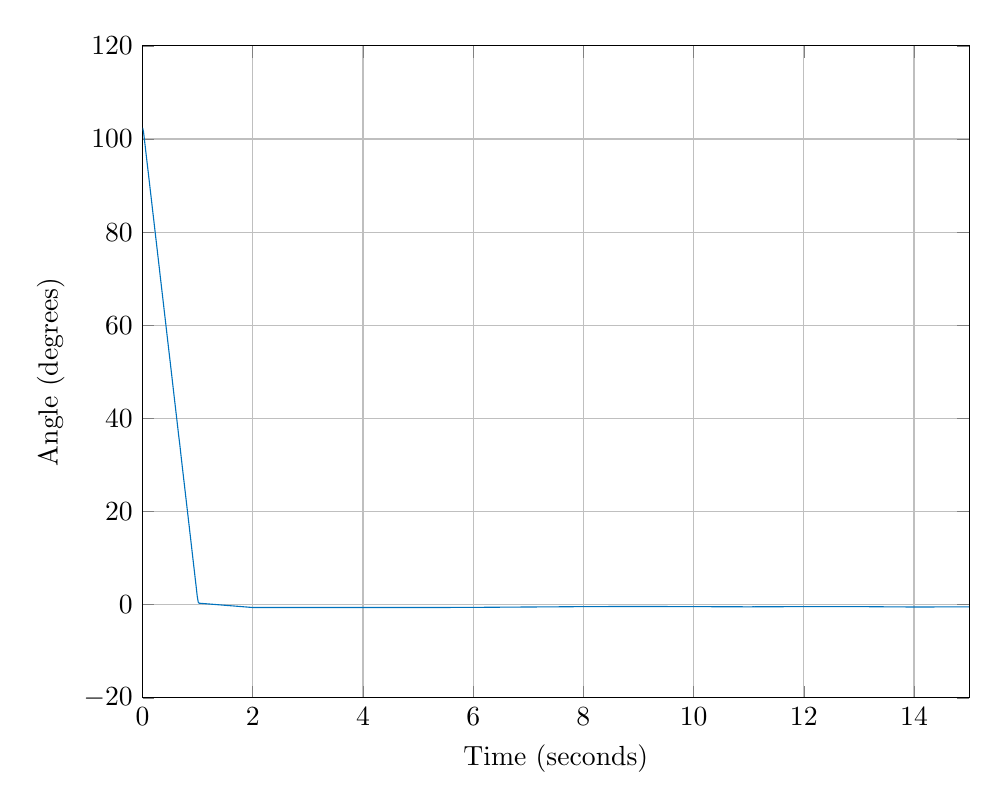
\begin{tikzpicture}

\begin{axis}[%
width=4.133in,
height=3.26in,
at={(0.693in,0.44in)},
scale only axis,
xmin=0,
xmax=15,
xmajorgrids,
xlabel={Time (seconds)},
ymin=-20,
ymax=120,
ymajorgrids,
ylabel={Angle (degrees)},
axis background/.style={fill=white}
]
\addplot [color=mycolor1,solid,forget plot]
  table[row sep=crcr]{%
0	102.4204\\
0.0174364199999999	101.5544\\
0.0324413389999997	100.0424\\
0.0480745519989999	98.4444\\
0.0640998179989997	96.7824\\
0.0802082269989997	95.1624\\
0.0962292989999996	93.5344\\
0.112140156998999	91.9224\\
0.128197941	90.2964\\
0.144129229999999	88.6344\\
0.160211415	87.0184\\
0.176086827998999	85.3564\\
0.192200153	83.7364\\
0.208225839	82.1044\\
0.224227045999	80.4664\\
0.240080554	78.8344\\
0.256212316	77.1944\\
0.272087498	75.5624\\
0.287968980998999	73.9284\\
0.304175280999999	72.2944\\
0.320220736	70.5924\\
0.336536562	68.9704\\
0.352217476999	67.3464\\
0.368193181	65.7424\\
0.384155161001	64.1064\\
0.400024181	62.4684\\
0.415951047999999	60.8544\\
0.431919778999	59.2064\\
0.447973876999999	57.5584\\
0.464059460999	55.9184\\
0.480058576	54.2984\\
0.496060176999	52.6744\\
0.512173605	51.0444\\
0.528068001999999	49.4124\\
0.544010151	47.7564\\
0.559998673	46.1064\\
0.576011581999999	44.4624\\
0.591989840999001	42.8464\\
0.608012696998999	41.1984\\
0.624180601999001	39.5624\\
0.640136015	37.9184\\
0.655922871	36.2824\\
0.674092178999	34.5824\\
0.689323626999999	32.9744\\
0.704526350000001	31.3604\\
0.720011259000001	29.7284\\
0.736073612999999	28.1104\\
0.752035972	26.4784\\
0.768029434998999	24.8544\\
0.784062675	23.2164\\
0.799996894999	21.5684\\
0.816036227998999	19.9424\\
0.832063142999	18.3104\\
0.848087181999999	16.6724\\
0.864017762999999	15.0324\\
0.880263498999	13.3904\\
0.896149981	11.7404\\
0.911956988998999	10.1104\\
0.928179579998999	8.45439999999999\\
0.944204442999999	6.81440000000001\\
0.960016884999	5.1844\\
0.976101866998999	3.5664\\
0.992018666999	1.87039999999999\\
1.010025436999	0.572399999999988\\
1.025319382	0.316400000000002\\
1.040847788	0.300399999999996\\
1.056282832	0.284399999999977\\
1.072203170999	0.27239999999999\\
1.088214014	0.256399999999985\\
1.10410021	0.240399999999994\\
1.120184143999	0.224399999999989\\
1.136192742999	0.212399999999974\\
1.153332650999	0.194400000000002\\
1.169049851999	0.180399999999992\\
1.184664222999	0.164400000000001\\
1.200207943999	0.148399999999995\\
1.216198867	0.136399999999981\\
1.232058714	0.120399999999989\\
1.248018682	0.104399999999984\\
1.264163278999	0.0884000000000071\\
1.280203778999	0.0723999999999876\\
1.296205294999	0.0583999999999776\\
1.312056418999	0.044399999999996\\
1.328273238999	0.0283999999999907\\
1.34413268	0.0123999999999853\\
1.36020774	-0.00360000000000582\\
1.376078550999	-0.0176000000000158\\
1.392107234999	-0.0315999999999974\\
1.408105734	-0.047600000000017\\
1.424191177	-0.0636000000000223\\
1.439961965999	-0.0795999999999992\\
1.455935304	-0.0936000000000092\\
1.47206816	-0.107600000000005\\
1.488172840999	-0.12360000000001\\
1.504562021999	-0.139600000000016\\
1.520175550999	-0.155600000000007\\
1.536107556	-0.171600000000012\\
1.552158274999	-0.183599999999998\\
1.568218684999	-0.199600000000004\\
1.584080896999	-0.215600000000023\\
1.600417683999	-0.2316\\
1.616165892999	-0.247600000000006\\
1.632020097999	-0.259600000000006\\
1.64800708	-0.275600000000011\\
1.663921684	-0.291600000000017\\
1.679974225	-0.307600000000008\\
1.696183247	-0.323600000000013\\
1.712205491999	-0.337600000000023\\
1.728202698	-0.351600000000005\\
1.74413995	-0.36760000000001\\
1.760297773	-0.383600000000001\\
1.776070962999	-0.399600000000007\\
1.792014729999	-0.413600000000017\\
1.808010689999	-0.427600000000012\\
1.824178137999	-0.443600000000018\\
1.840175485999	-0.459599999999995\\
1.856258517999	-0.475600000000014\\
1.872046412	-0.489600000000024\\
1.888057365999	-0.503600000000006\\
1.903962273	-0.519600000000011\\
1.920177224999	-0.535600000000002\\
1.936126995999	-0.551600000000008\\
1.952091072999	-0.565600000000018\\
1.968175580999	-0.579599999999999\\
1.984195162	-0.595600000000019\\
2.000203769999	-0.611599999999996\\
2.017723236	-0.61960000000002\\
2.03286175	-0.61960000000002\\
2.047944468	-0.61960000000002\\
2.063966206	-0.61960000000002\\
2.079946495999	-0.61960000000002\\
2.098116071999	-0.61960000000002\\
2.113148563999	-0.61960000000002\\
2.128386502	-0.61960000000002\\
2.144113648	-0.61960000000002\\
2.159934625999	-0.61960000000002\\
2.17611003	-0.61960000000002\\
2.19209383	-0.61960000000002\\
2.208082964	-0.61960000000002\\
2.224121148999	-0.61960000000002\\
2.240056938	-0.61960000000002\\
2.256037618	-0.61960000000002\\
2.274214714	-0.61960000000002\\
2.289394059	-0.61960000000002\\
2.30458258	-0.61960000000002\\
2.320164677999	-0.61960000000002\\
2.337081984	-0.61960000000002\\
2.35244274	-0.61960000000002\\
2.368217484	-0.61960000000002\\
2.384157628001	-0.61960000000002\\
2.400174926	-0.61960000000002\\
2.416436913	-0.61960000000002\\
2.432192117999	-0.61960000000002\\
2.448213056	-0.61960000000002\\
2.463979465	-0.61960000000002\\
2.480214109999	-0.61960000000002\\
2.496150904	-0.61960000000002\\
2.51202091	-0.61960000000002\\
2.528092401	-0.61960000000002\\
2.544057696	-0.61960000000002\\
2.560052073	-0.61960000000002\\
2.576022575	-0.61960000000002\\
2.592061983	-0.61960000000002\\
2.608066929	-0.61960000000002\\
2.624044757	-0.61960000000002\\
2.640132328999	-0.61960000000002\\
2.656117033999	-0.61960000000002\\
2.67206056	-0.61960000000002\\
2.688063049	-0.61960000000002\\
2.704059540999	-0.61960000000002\\
2.720050849	-0.61960000000002\\
2.736020509999	-0.61960000000002\\
2.752026533	-0.61960000000002\\
2.768011547999	-0.61960000000002\\
2.784059405999	-0.61960000000002\\
2.800047727999	-0.61960000000002\\
2.816122816999	-0.61960000000002\\
2.832212373999	-0.61960000000002\\
2.848164019	-0.61960000000002\\
2.864079035	-0.61960000000002\\
2.880064906999	-0.61960000000002\\
2.895952181999	-0.61960000000002\\
2.912846776	-0.61960000000002\\
2.928184557999	-0.61960000000002\\
2.944053722999	-0.61960000000002\\
2.960053562	-0.61960000000002\\
2.975999719	-0.61960000000002\\
2.994254925999	-0.61960000000002\\
3.008585559999	-0.61960000000002\\
3.024117377	-0.61960000000002\\
3.040093882999	-0.61960000000002\\
3.056201951999	-0.61960000000002\\
3.072171406	-0.61960000000002\\
3.088090247	-0.61960000000002\\
3.104069609	-0.61960000000002\\
3.120078504	-0.61960000000002\\
3.136031345001	-0.61960000000002\\
3.151960363999	-0.61960000000002\\
3.168030761999	-0.61960000000002\\
3.184088748	-0.61960000000002\\
3.200043123999	-0.61960000000002\\
3.216096242999	-0.61960000000002\\
3.232345321	-0.61960000000002\\
3.248246571	-0.61960000000002\\
3.264068767999	-0.61960000000002\\
3.280051673	-0.61960000000002\\
3.296060010999	-0.61960000000002\\
3.312053810999	-0.61960000000002\\
3.328149971999	-0.61960000000002\\
3.344134951999	-0.61960000000002\\
3.359977662999	-0.61960000000002\\
3.378183431	-0.61960000000002\\
3.393311515	-0.61960000000002\\
3.408329681	-0.61960000000002\\
3.423965118999	-0.61960000000002\\
3.440091207998	-0.61960000000002\\
3.456068635999	-0.61960000000002\\
3.472002359999	-0.61960000000002\\
3.488001425	-0.61960000000002\\
3.50399475	-0.61960000000002\\
3.520059731999	-0.61960000000002\\
3.536060682999	-0.61960000000002\\
3.552030617999	-0.61960000000002\\
3.568062920999	-0.61960000000002\\
3.584051137999	-0.61960000000002\\
3.600061967	-0.61960000000002\\
3.616100809	-0.61960000000002\\
3.632072217999	-0.61960000000002\\
3.648039532	-0.61960000000002\\
3.664712465999	-0.61960000000002\\
3.680096951	-0.61960000000002\\
3.695980576999	-0.61960000000002\\
3.712197562	-0.61960000000002\\
3.728204576999	-0.61960000000002\\
3.744034690999	-0.61960000000002\\
3.760202780999	-0.61960000000002\\
3.776177844	-0.61960000000002\\
3.792106691	-0.61960000000002\\
3.808257335999	-0.61960000000002\\
3.824203394	-0.61960000000002\\
3.840289837999	-0.61960000000002\\
3.856198254999	-0.61960000000002\\
3.872320295	-0.61960000000002\\
3.888010259	-0.61960000000002\\
3.903925231999	-0.61960000000002\\
3.920045058999	-0.61960000000002\\
3.936110399	-0.61960000000002\\
3.952102193	-0.61960000000002\\
3.967993017	-0.61960000000002\\
3.984011323	-0.61960000000002\\
4.000032677999	-0.61960000000002\\
4.017330059	-0.61960000000002\\
4.032641609	-0.61960000000002\\
4.048226707	-0.61960000000002\\
4.064199278999	-0.61960000000002\\
4.080152432999	-0.61960000000002\\
4.096619945999	-0.61960000000002\\
4.112303497	-0.61960000000002\\
4.128193923	-0.61960000000002\\
4.144085671	-0.61960000000002\\
4.159940774	-0.61960000000002\\
4.177991844	-0.61960000000002\\
4.192873846999	-0.61960000000002\\
4.208390108	-0.61960000000002\\
4.224197497	-0.61960000000002\\
4.240197639999	-0.61960000000002\\
4.256212827999	-0.61960000000002\\
4.272338436999	-0.61960000000002\\
4.288223765999	-0.61960000000002\\
4.304298875	-0.61960000000002\\
4.320226073999	-0.61960000000002\\
4.338806023	-0.61960000000002\\
4.35426679	-0.61960000000002\\
4.369876093999	-0.61960000000002\\
4.385399932999	-0.61960000000002\\
4.4010598	-0.61960000000002\\
4.416364753001	-0.61960000000002\\
4.432178811	-0.61960000000002\\
4.448292142	-0.61960000000002\\
4.464212710999	-0.61960000000002\\
4.480030828	-0.61960000000002\\
4.496202891	-0.61960000000002\\
4.512198484999	-0.61960000000002\\
4.528154323999	-0.61960000000002\\
4.544188686	-0.61960000000002\\
4.560194137999	-0.61960000000002\\
4.576274293	-0.61960000000002\\
4.592259242999	-0.61960000000002\\
4.608199813	-0.61960000000002\\
4.624300734999	-0.61960000000002\\
4.64027266	-0.61960000000002\\
4.656180592	-0.61960000000002\\
4.672191971	-0.61960000000002\\
4.688079760999	-0.61960000000002\\
4.704200662999	-0.61960000000002\\
4.720204184	-0.61960000000002\\
4.736184309999	-0.61960000000002\\
4.752069476999	-0.61960000000002\\
4.768200349	-0.61960000000002\\
4.784186788999	-0.61960000000002\\
4.800115549998	-0.61960000000002\\
4.816082899999	-0.61960000000002\\
4.832065785	-0.61960000000002\\
4.848044270999	-0.61960000000002\\
4.864202106999	-0.61960000000002\\
4.880229006999	-0.61960000000002\\
4.896204436	-0.61960000000002\\
4.912107910999	-0.61960000000002\\
4.928169884999	-0.61960000000002\\
4.944215616999	-0.61960000000002\\
4.960190734	-0.61960000000002\\
4.976067642	-0.61960000000002\\
4.992011913999	-0.61960000000002\\
5.009937497	-0.61960000000002\\
5.024994391998	-0.61960000000002\\
5.040080075	-0.61760000000001\\
5.056301701	-0.61760000000001\\
5.072096184999	-0.61760000000001\\
5.088119672	-0.615600000000015\\
5.1041215	-0.615600000000015\\
5.12031192	-0.615600000000015\\
5.136008354999	-0.613600000000019\\
5.152018478999	-0.613600000000019\\
5.168155486999	-0.613600000000019\\
5.184126971999	-0.611599999999996\\
5.200222323	-0.611599999999996\\
5.216202545999	-0.611599999999996\\
5.232202991999	-0.611599999999996\\
5.248138389	-0.6096\\
5.264081293999	-0.6096\\
5.280199671	-0.6096\\
5.296137108	-0.607600000000005\\
5.312170363	-0.607600000000005\\
5.328191163999	-0.607600000000005\\
5.344200639999	-0.60560000000001\\
5.360208571999	-0.60560000000001\\
5.37619716	-0.60560000000001\\
5.392456622	-0.6036\\
5.409543821999	-0.6036\\
5.425040842999	-0.6036\\
5.440446882	-0.601600000000005\\
5.456213241	-0.601600000000005\\
5.472084109	-0.601600000000005\\
5.488205918	-0.599600000000009\\
5.504746311	-0.599600000000009\\
5.520214770999	-0.599600000000009\\
5.536072732	-0.599600000000009\\
5.552104776	-0.597600000000014\\
5.568203873	-0.597600000000014\\
5.584268137999	-0.597600000000014\\
5.600219861999	-0.595600000000019\\
5.616093009	-0.595600000000019\\
5.63218009	-0.595600000000019\\
5.648047674	-0.593600000000009\\
5.663950050999	-0.593600000000009\\
5.680101163999	-0.593600000000009\\
5.696208217	-0.591600000000014\\
5.712189446999	-0.591600000000014\\
5.728124238	-0.591600000000014\\
5.744016382999	-0.589600000000019\\
5.759969333	-0.589600000000019\\
5.776390062	-0.589600000000019\\
5.792203684	-0.587599999999995\\
5.808111793	-0.587599999999995\\
5.824230427999	-0.587599999999995\\
5.840264067999	-0.585599999999999\\
5.85619913	-0.585599999999999\\
5.872219665999	-0.585599999999999\\
5.888061250999	-0.585599999999999\\
5.904005122	-0.583600000000004\\
5.920174464999	-0.583600000000004\\
5.936176504	-0.583600000000004\\
5.952099142	-0.581600000000009\\
5.968218316999	-0.581600000000009\\
5.984208788999	-0.581600000000009\\
6.000112769999	-0.579599999999999\\
6.017582649	-0.579599999999999\\
6.032675724	-0.579599999999999\\
6.04809412	-0.575600000000009\\
6.064063339999	-0.575600000000009\\
6.080053071	-0.575600000000009\\
6.096028728999	-0.571599999999989\\
6.112248274999	-0.571599999999989\\
6.128208428999	-0.571599999999989\\
6.14396666	-0.569599999999994\\
6.159953748999	-0.567599999999999\\
6.176064281	-0.567599999999999\\
6.192075689999	-0.567599999999999\\
6.208060142999	-0.563599999999994\\
6.224060497999	-0.563599999999994\\
6.240172138999	-0.563599999999994\\
6.256208938	-0.559600000000003\\
6.272330718	-0.559600000000003\\
6.288081672	-0.559600000000003\\
6.30405878	-0.555599999999998\\
6.320175488	-0.555599999999998\\
6.336359641	-0.555599999999998\\
6.352202451999	-0.551600000000008\\
6.368325165	-0.551600000000008\\
6.384229085999	-0.551600000000008\\
6.399927596999	-0.547600000000017\\
6.418094974999	-0.547600000000017\\
6.433175913	-0.547600000000017\\
6.448245408999	-0.545600000000007\\
6.464020657999	-0.543599999999998\\
6.480112335999	-0.543599999999998\\
6.496167585	-0.541599999999988\\
6.512213201999	-0.539599999999993\\
6.528219730999	-0.539599999999993\\
6.544099521999	-0.539599999999993\\
6.560153358	-0.535600000000002\\
6.576187239	-0.535600000000002\\
6.591977611	-0.535600000000002\\
6.608326035999	-0.531599999999997\\
6.624058384	-0.531599999999997\\
6.640218780999	-0.531599999999997\\
6.655994672	-0.527600000000007\\
6.672041295999	-0.527600000000007\\
6.688202523	-0.527600000000007\\
6.704048743999	-0.523600000000016\\
6.720080634999	-0.523600000000016\\
6.736160679	-0.523600000000016\\
6.752048283	-0.519599999999997\\
6.768064769999	-0.519599999999997\\
6.784071057999	-0.519599999999997\\
6.800020132	-0.517599999999987\\
6.816298351	-0.515599999999992\\
6.832204156999	-0.515599999999992\\
6.848177184999	-0.515599999999992\\
6.864213294999	-0.511600000000001\\
6.880201443	-0.511600000000001\\
6.896166096999	-0.511600000000001\\
6.911979625999	-0.507599999999996\\
6.92806041	-0.507599999999996\\
6.944051668999	-0.507599999999996\\
6.960060702999	-0.503600000000006\\
6.976001891	-0.503600000000006\\
6.992188637	-0.503600000000006\\
7.009917887999	-0.499600000000015\\
7.025062535	-0.499600000000015\\
7.040364753001	-0.499600000000015\\
7.056003098	-0.495599999999996\\
7.072091451999	-0.495599999999996\\
7.088046931	-0.495599999999996\\
7.104099507999	-0.493599999999986\\
7.120061782	-0.491599999999991\\
7.136064551999	-0.491599999999991\\
7.151995634999	-0.489599999999996\\
7.170209929999	-0.4876\\
7.185489417	-0.4876\\
7.200828347999	-0.4876\\
7.21612082	-0.483599999999996\\
7.232095876999	-0.483599999999996\\
7.248067061	-0.483599999999996\\
7.264062109	-0.479600000000005\\
7.280057412	-0.479600000000005\\
7.296058128001	-0.479600000000005\\
7.312066129999	-0.475600000000014\\
7.328052112	-0.475600000000014\\
7.344019281	-0.475600000000014\\
7.359993398999	-0.471599999999995\\
7.376050155	-0.471599999999995\\
7.392077826999	-0.471599999999995\\
7.407967070999	-0.46759999999999\\
7.424091946999	-0.46759999999999\\
7.440058199	-0.46759999999999\\
7.456025599	-0.465599999999995\\
7.472217814	-0.4636\\
7.488063783999	-0.4636\\
7.504063803	-0.4636\\
7.520128848999	-0.459599999999995\\
7.536059997	-0.459599999999995\\
7.552213804999	-0.459599999999995\\
7.568210811999	-0.455600000000004\\
7.584116689999	-0.455600000000004\\
7.600213226	-0.455600000000004\\
7.616205160999	-0.451600000000013\\
7.632079521	-0.451600000000013\\
7.647950417	-0.451600000000013\\
7.666106786001	-0.447600000000008\\
7.681468854999	-0.447600000000008\\
7.696943389	-0.447600000000008\\
7.712615464	-0.443599999999989\\
7.728273618999	-0.443599999999989\\
7.744215101	-0.443599999999989\\
7.760236634	-0.441599999999994\\
7.776114829999	-0.439599999999999\\
7.792352809999	-0.439599999999999\\
7.808138939999	-0.437600000000003\\
7.824086795999	-0.435599999999994\\
7.840110754	-0.435599999999994\\
7.856078049	-0.435599999999994\\
7.872126637999	-0.431600000000003\\
7.888043507999	-0.431600000000003\\
7.903946002	-0.431600000000003\\
7.920086553999	-0.427600000000012\\
7.936316118	-0.427600000000012\\
7.952195795	-0.427600000000012\\
7.968162714	-0.423600000000008\\
7.984209183	-0.423600000000008\\
8.000211878001	-0.423600000000008\\
8.016028740999	-0.421600000000012\\
8.032065369	-0.421600000000012\\
8.048202825	-0.421600000000012\\
8.064173947999	-0.419600000000017\\
8.080183639	-0.419600000000017\\
8.096363681	-0.419600000000017\\
8.11214023	-0.417600000000022\\
8.128158209	-0.417600000000022\\
8.144422215999	-0.417600000000022\\
8.160094943999	-0.417600000000022\\
8.176183418	-0.415600000000012\\
8.192197979999	-0.415600000000012\\
8.208134901999	-0.415600000000012\\
8.224202899999	-0.413600000000017\\
8.240206561999	-0.413600000000017\\
8.256082894999	-0.413600000000017\\
8.272055693	-0.411600000000021\\
8.288083318999	-0.411600000000021\\
8.304080361999	-0.411600000000021\\
8.320199710999	-0.409599999999998\\
8.336408568	-0.409599999999998\\
8.352774370999	-0.409599999999998\\
8.368230387	-0.407600000000002\\
8.384177747	-0.407600000000002\\
8.400262842	-0.407600000000002\\
8.416117839999	-0.405600000000007\\
8.431974916	-0.405600000000007\\
8.448092601999	-0.405600000000007\\
8.464086698	-0.403600000000012\\
8.480081342999	-0.403600000000012\\
8.496115599999	-0.403600000000012\\
8.512198596999	-0.403600000000012\\
8.528179257	-0.401600000000002\\
8.544071862999	-0.401600000000002\\
8.560199276	-0.401600000000002\\
8.576202712	-0.399600000000007\\
8.592157599999	-0.399600000000007\\
8.608204613999	-0.399600000000007\\
8.624250753001	-0.397600000000011\\
8.640201991999	-0.397600000000011\\
8.655952028	-0.397600000000011\\
8.674264316	-0.395600000000016\\
8.690029313	-0.395600000000016\\
8.70533116	-0.395600000000016\\
8.720462252	-0.393600000000021\\
8.736054311	-0.393600000000021\\
8.752167026	-0.393600000000021\\
8.768216337	-0.391600000000011\\
8.784117234999	-0.391600000000011\\
8.800222247999	-0.391600000000011\\
8.816085878001	-0.391600000000011\\
8.832200255999	-0.389600000000016\\
8.848208899999	-0.389600000000016\\
8.864074028	-0.389600000000016\\
8.879972388999	-0.38760000000002\\
8.898176418999	-0.38760000000002\\
8.913392229999	-0.38760000000002\\
8.92820018	-0.385600000000025\\
8.944193965	-0.385600000000025\\
8.960134269	-0.385600000000025\\
8.976188917	-0.383600000000001\\
8.99227928	-0.383600000000001\\
9.010184870999	-0.383600000000001\\
9.02539478	-0.385599999999997\\
9.040911420999	-0.385599999999997\\
9.056161129	-0.385599999999997\\
9.072005068999	-0.387599999999992\\
9.088078109	-0.387599999999992\\
9.104068896999	-0.387599999999992\\
9.120023436	-0.389600000000002\\
9.136077655	-0.389600000000002\\
9.151989933	-0.389600000000002\\
9.168026231	-0.389600000000002\\
9.184192672	-0.391599999999997\\
9.200145398999	-0.391599999999997\\
9.216075017999	-0.391599999999997\\
9.232121800999	-0.393599999999992\\
9.248089691999	-0.393599999999992\\
9.264096814999	-0.393599999999992\\
9.280090168	-0.395600000000016\\
9.295993071999	-0.395600000000016\\
9.314136978	-0.395600000000016\\
9.329233987	-0.397600000000011\\
9.344568609999	-0.397600000000011\\
9.360134695	-0.397600000000011\\
9.376179540999	-0.399600000000007\\
9.392306382	-0.399600000000007\\
9.407975764	-0.399600000000007\\
9.424032971	-0.401600000000002\\
9.440175618	-0.401600000000002\\
9.456204844	-0.401600000000002\\
9.47216182	-0.401600000000002\\
9.488058073999	-0.403600000000012\\
9.504047424	-0.403600000000012\\
9.520006595001	-0.403600000000012\\
9.536055745999	-0.405600000000007\\
9.552117752999	-0.405600000000007\\
9.568094486	-0.405600000000007\\
9.584199884999	-0.407600000000002\\
9.600003557	-0.407600000000002\\
9.615998725	-0.407600000000002\\
9.632118151999	-0.409599999999998\\
9.648181718999	-0.409599999999998\\
9.6641735	-0.409599999999998\\
9.680241717999	-0.411599999999993\\
9.696210542	-0.411599999999993\\
9.712220362999	-0.411599999999993\\
9.728217976	-0.413600000000002\\
9.744161601999	-0.413600000000002\\
9.760112507	-0.413600000000002\\
9.776056043999	-0.415599999999998\\
9.792012257	-0.415599999999998\\
9.807986535	-0.415599999999998\\
9.824083686	-0.415599999999998\\
9.840049543	-0.417599999999993\\
9.856053837	-0.417599999999993\\
9.87206002	-0.417599999999993\\
9.888050457	-0.419599999999988\\
9.903937345001	-0.419599999999988\\
9.922163447	-0.419599999999988\\
9.937634653	-0.421600000000012\\
9.953129364	-0.421600000000012\\
9.968507009	-0.421600000000012\\
9.984406637999	-0.423600000000008\\
10.000217073	-0.423600000000008\\
10.017969955	-0.423600000000008\\
10.033488119999	-0.425600000000003\\
10.048571818	-0.425600000000003\\
10.064066002	-0.425600000000003\\
10.080080618999	-0.427600000000012\\
10.096186568	-0.427600000000012\\
10.112210625999	-0.427600000000012\\
10.128145726	-0.429600000000008\\
10.144204910999	-0.429600000000008\\
10.159938590999	-0.429600000000008\\
10.176176891	-0.429600000000008\\
10.192216039	-0.431600000000003\\
10.208161094	-0.431600000000003\\
10.224046457	-0.431600000000003\\
10.240191195	-0.433599999999998\\
10.25609008	-0.433599999999998\\
10.272064229999	-0.433599999999998\\
10.288082545999	-0.435599999999994\\
10.304050887999	-0.435599999999994\\
10.319991915999	-0.435599999999994\\
10.336056162999	-0.437600000000003\\
10.352059774999	-0.437600000000003\\
10.368178226999	-0.437600000000003\\
10.384231177	-0.439599999999999\\
10.400195154	-0.439599999999999\\
10.416024529	-0.439599999999999\\
10.432109223999	-0.441599999999994\\
10.448068096	-0.441599999999994\\
10.464246115	-0.441599999999994\\
10.480207807999	-0.441599999999994\\
10.496232162	-0.443599999999989\\
10.512324549998	-0.443599999999989\\
10.528215467	-0.443599999999989\\
10.544222823	-0.445600000000013\\
10.560126141	-0.445600000000013\\
10.576121762	-0.445600000000013\\
10.592047838	-0.447600000000008\\
10.608060882	-0.447600000000008\\
10.624047891998	-0.447600000000008\\
10.640089960999	-0.449600000000004\\
10.656113156999	-0.449600000000004\\
10.672093887999	-0.449600000000004\\
10.688308031999	-0.451600000000013\\
10.704151377	-0.451600000000013\\
10.720198939	-0.451600000000013\\
10.736174438	-0.453600000000009\\
10.752210641	-0.453600000000009\\
10.768198273	-0.453600000000009\\
10.784261927	-0.455600000000004\\
10.800130243999	-0.455600000000004\\
10.816293451	-0.455600000000004\\
10.832309474	-0.455600000000004\\
10.848255181	-0.457599999999999\\
10.864332035999	-0.457599999999999\\
10.880404217999	-0.457599999999999\\
10.896335146999	-0.459599999999995\\
10.911954291	-0.459599999999995\\
10.92818571	-0.459599999999995\\
10.943977613999	-0.461600000000004\\
10.960189547999	-0.461600000000004\\
10.976184509999	-0.461600000000004\\
10.992134073999	-0.4636\\
11.008082330999	-0.461600000000004\\
11.024231929	-0.459599999999995\\
11.040197245	-0.459599999999995\\
11.056075523	-0.461600000000004\\
11.072125294999	-0.457599999999999\\
11.088084674	-0.457599999999999\\
11.104015208999	-0.459599999999995\\
11.120054285999	-0.455600000000004\\
11.136115278	-0.455600000000004\\
11.152140017	-0.457599999999999\\
11.167985531999	-0.455600000000004\\
11.184181004	-0.453600000000009\\
11.200179856	-0.455600000000004\\
11.216176351999	-0.453600000000009\\
11.23215628	-0.451600000000013\\
11.248217498	-0.453600000000009\\
11.26421231	-0.451600000000013\\
11.280067560999	-0.44959999999999\\
11.296085229999	-0.44959999999999\\
11.312042231999	-0.449600000000004\\
11.328179461999	-0.447600000000008\\
11.3446142	-0.447600000000008\\
11.360203604	-0.449600000000004\\
11.376146488	-0.445600000000013\\
11.392205656999	-0.445600000000013\\
11.407981149	-0.447600000000008\\
11.423929568999	-0.443599999999989\\
11.440186409	-0.443599999999989\\
11.456194918999	-0.445599999999985\\
11.472014035	-0.443599999999989\\
11.488117798	-0.441599999999994\\
11.504316311999	-0.443599999999989\\
11.520250436	-0.441599999999994\\
11.536185748	-0.439599999999999\\
11.552139262	-0.441599999999994\\
11.568174371	-0.439599999999999\\
11.584267846	-0.437600000000003\\
11.600248576999	-0.437600000000003\\
11.616204946999	-0.437600000000003\\
11.63221312	-0.435599999999994\\
11.648209941	-0.435599999999994\\
11.663996004	-0.435599999999994\\
11.680128519999	-0.433599999999998\\
11.696163823999	-0.433599999999998\\
11.712303564999	-0.435599999999994\\
11.728084547	-0.431600000000003\\
11.744057790999	-0.431600000000003\\
11.760244778	-0.433599999999998\\
11.776229196999	-0.429600000000008\\
11.792264014999	-0.429600000000008\\
11.808331186	-0.431600000000003\\
11.825191298	-0.427600000000012\\
11.840621656999	-0.427600000000012\\
11.856223063	-0.429600000000008\\
11.872230283999	-0.427600000000012\\
11.888200314999	-0.425599999999989\\
11.904167559999	-0.427599999999984\\
11.920138774	-0.425599999999989\\
11.936170007999	-0.423599999999993\\
11.952202912	-0.425600000000003\\
11.968161111	-0.423600000000008\\
11.984070997	-0.421600000000012\\
12.000056677999	-0.421600000000012\\
12.017315042	-0.423600000000008\\
12.032281806	-0.423600000000008\\
12.048081410999	-0.423600000000008\\
12.064308474	-0.423600000000008\\
12.080278104	-0.423600000000008\\
12.096073921	-0.423600000000008\\
12.112073715	-0.423600000000008\\
12.128202931	-0.423600000000008\\
12.144180404	-0.423600000000008\\
12.160081519	-0.423600000000008\\
12.176206906999	-0.423600000000008\\
12.192068107	-0.423600000000008\\
12.208199363	-0.423600000000008\\
12.22407479	-0.423600000000008\\
12.240057064	-0.423600000000008\\
12.256054823	-0.423600000000008\\
12.2720362	-0.423600000000008\\
12.288030491	-0.423600000000008\\
12.304027457998	-0.423600000000008\\
12.320016186999	-0.423600000000008\\
12.336050924	-0.423600000000008\\
12.352062083	-0.423600000000008\\
12.368033031999	-0.423600000000008\\
12.384199802999	-0.423600000000008\\
12.400176484999	-0.423600000000008\\
12.415988171999	-0.423600000000008\\
12.432075977999	-0.423600000000008\\
12.448216396999	-0.423600000000008\\
12.464242686	-0.423600000000008\\
12.480121139	-0.423600000000008\\
12.496033755	-0.423600000000008\\
12.512193856999	-0.423600000000008\\
12.528225082	-0.423600000000008\\
12.544176526	-0.423600000000008\\
12.560273396	-0.423600000000008\\
12.576195802999	-0.423600000000008\\
12.592181449	-0.423600000000008\\
12.608272439999	-0.423600000000008\\
12.624093889	-0.423600000000008\\
12.640066861999	-0.423600000000008\\
12.6559628	-0.423600000000008\\
12.672079446999	-0.423600000000008\\
12.688097774	-0.423600000000008\\
12.704333130999	-0.423600000000008\\
12.720306903	-0.423600000000008\\
12.736221915	-0.423600000000008\\
12.752089722999	-0.423600000000008\\
12.768073213	-0.423600000000008\\
12.783995431	-0.423600000000008\\
12.800007804999	-0.423600000000008\\
12.816050023	-0.423600000000008\\
12.83209339	-0.423600000000008\\
12.848042714	-0.423600000000008\\
12.864146927	-0.423600000000008\\
12.880118554	-0.423600000000008\\
12.896110917	-0.423600000000008\\
12.91206448	-0.423600000000008\\
12.928080915999	-0.423600000000008\\
12.944202627	-0.423600000000008\\
12.960184784	-0.423600000000008\\
12.976024661001	-0.423600000000008\\
12.992227343999	-0.423600000000008\\
13.010088955	-0.423600000000008\\
13.025480401	-0.423600000000008\\
13.040947026	-0.427600000000012\\
13.056400221999	-0.427600000000012\\
13.072421052999	-0.427600000000012\\
13.088182045999	-0.429600000000008\\
13.104083917	-0.431600000000003\\
13.120068872	-0.431600000000003\\
13.13606193	-0.433599999999998\\
13.152128434999	-0.435599999999994\\
13.168114924	-0.435599999999994\\
13.184053543	-0.435599999999994\\
13.200015246	-0.439600000000013\\
13.216070555	-0.439600000000013\\
13.232188236	-0.439600000000013\\
13.248141116999	-0.443600000000018\\
13.26421102	-0.443600000000018\\
13.280210879	-0.443600000000018\\
13.296234049998	-0.447600000000008\\
13.312201075	-0.447600000000008\\
13.328236222999	-0.447600000000008\\
13.344222486	-0.451600000000013\\
13.360206333999	-0.451600000000013\\
13.376192356	-0.451600000000013\\
13.392119818999	-0.455600000000004\\
13.407962903999	-0.455600000000004\\
13.426396255999	-0.455600000000004\\
13.441892443	-0.457599999999999\\
13.457407142999	-0.459599999999995\\
13.472815811999	-0.459599999999995\\
13.488056892999	-0.461600000000004\\
13.504058335	-0.4636\\
13.520110141	-0.4636\\
13.536202068	-0.4636\\
13.552206391998	-0.46759999999999\\
13.568088538999	-0.46759999999999\\
13.584002033999	-0.46759999999999\\
13.600041446	-0.471600000000009\\
13.616008505	-0.471600000000009\\
13.631974613999	-0.471600000000009\\
13.648012806	-0.475600000000014\\
13.663901446999	-0.475600000000014\\
13.680061205	-0.475600000000014\\
13.69632314	-0.479600000000005\\
13.712179460999	-0.479600000000005\\
13.728084750999	-0.479600000000005\\
13.743986149999	-0.4816\\
13.760055311999	-0.483599999999996\\
13.776062998999	-0.483599999999996\\
13.792184378001	-0.485600000000005\\
13.808313684999	-0.487600000000015\\
13.824265479999	-0.487600000000015\\
13.840226965999	-0.487600000000015\\
13.856213990999	-0.49160000000002\\
13.872097174998	-0.49160000000002\\
13.888206016	-0.49160000000002\\
13.904039655	-0.49560000000001\\
13.919964221	-0.49560000000001\\
13.936103005	-0.49560000000001\\
13.952180613999	-0.499600000000015\\
13.968192709	-0.499600000000015\\
13.984070132	-0.499600000000015\\
14.000051488999	-0.503600000000006\\
14.016011151999	-0.503600000000006\\
14.034246443999	-0.50160000000001\\
14.049343563	-0.50160000000001\\
14.064405297	-0.50160000000001\\
14.080171981999	-0.499600000000015\\
14.096061645999	-0.499600000000015\\
14.112229215	-0.499600000000015\\
14.128208261	-0.497599999999991\\
14.144170935999	-0.497599999999991\\
14.160048948999	-0.497599999999991\\
14.17606949	-0.495599999999996\\
14.192172597	-0.495599999999996\\
14.208240257	-0.495599999999996\\
14.224071500999	-0.495599999999996\\
14.240099358	-0.493599999999986\\
14.256054384999	-0.493599999999986\\
14.27218038	-0.493599999999986\\
14.288206633	-0.491599999999991\\
14.304213702999	-0.491599999999991\\
14.320425275999	-0.491599999999991\\
14.33652227	-0.489599999999996\\
14.352191584999	-0.489599999999996\\
14.368370188	-0.489599999999996\\
14.384222978999	-0.4876\\
14.400103646999	-0.4876\\
14.416020157999	-0.4876\\
14.431916567	-0.485600000000005\\
14.448193839	-0.485600000000005\\
14.464190675999	-0.485600000000005\\
14.480051981	-0.483599999999996\\
14.496002953999	-0.483599999999996\\
14.512052755999	-0.483599999999996\\
14.528050965999	-0.483599999999996\\
14.544508546	-0.4816\\
14.560222451999	-0.4816\\
14.576060674998	-0.4816\\
14.592227091	-0.479600000000005\\
14.6082781	-0.479600000000005\\
14.624190004999	-0.479600000000005\\
14.640100294999	-0.47760000000001\\
14.655963758	-0.47760000000001\\
14.67435481	-0.47760000000001\\
14.689904813	-0.475600000000014\\
14.705240781999	-0.475600000000014\\
14.720675092999	-0.475600000000014\\
14.7361544	-0.473600000000005\\
14.752174096	-0.473600000000005\\
14.768177503001	-0.473600000000005\\
14.784122136999	-0.471600000000009\\
14.800116461	-0.471600000000009\\
14.816190267999	-0.471600000000009\\
14.83196707	-0.469600000000014\\
14.847890165	-0.469600000000014\\
14.866124297	-0.469600000000014\\
14.881334130999	-0.467600000000019\\
14.896480326	-0.467600000000019\\
14.911933860999	-0.467600000000019\\
14.928071076999	-0.467600000000019\\
14.944316551999	-0.465600000000023\\
14.960207469	-0.465600000000023\\
14.9761995	-0.465600000000023\\
14.992234368	-0.463600000000014\\
15.008099286001	-0.461600000000018\\
15.024100913	-0.461600000000018\\
15.040066068999	-0.459600000000023\\
15.056057943999	-0.459600000000023\\
15.072058004	-0.457600000000028\\
15.088056785	-0.455600000000032\\
15.103969566	-0.455600000000032\\
15.120139771999	-0.453600000000023\\
15.136092712999	-0.451600000000013\\
15.152243794999	-0.451600000000013\\
15.168113941999	-0.44959999999999\\
15.184102256999	-0.44959999999999\\
15.200057688	-0.447599999999994\\
15.216106825	-0.445599999999985\\
15.232155876	-0.445599999999985\\
15.248052339999	-0.443599999999989\\
15.264006459	-0.441599999999994\\
15.280059804999	-0.441599999999994\\
15.296075844999	-0.439599999999999\\
15.312006465	-0.437600000000003\\
15.328084943999	-0.437600000000003\\
15.344091292	-0.435599999999994\\
15.360216309	-0.435599999999994\\
15.376174509	-0.433599999999998\\
15.392242703	-0.431600000000003\\
15.408148096999	-0.431600000000003\\
15.424129934999	-0.429600000000008\\
15.440208695999	-0.427600000000012\\
15.456158507999	-0.427600000000012\\
15.472113941	-0.425600000000003\\
15.488208599	-0.423600000000008\\
15.504318838	-0.423600000000008\\
15.520073346	-0.421600000000012\\
15.53606457	-0.421600000000012\\
15.552151961999	-0.419600000000017\\
15.568169015	-0.417600000000022\\
15.584234967	-0.417600000000022\\
15.599992284999	-0.415600000000012\\
15.616203329999	-0.413600000000017\\
15.632208891	-0.413600000000017\\
15.648360293999	-0.411600000000021\\
15.663979619999	-0.411600000000021\\
15.680206142	-0.409600000000026\\
15.696039139999	-0.407600000000031\\
15.712021123	-0.407600000000031\\
15.728025839999	-0.405600000000021\\
15.743955066999	-0.403600000000026\\
15.759945672	-0.403600000000026\\
15.775934901999	-0.40160000000003\\
15.791938962999	-0.399600000000007\\
15.808067960999	-0.399600000000007\\
15.824084071999	-0.397599999999983\\
15.840209351999	-0.397599999999983\\
15.856185299	-0.395599999999988\\
15.872097137999	-0.393599999999992\\
15.888054205	-0.393599999999992\\
15.904087638	-0.391599999999997\\
15.92043274	-0.389600000000002\\
15.93625657	-0.389600000000002\\
15.951973564999	-0.387599999999992\\
15.96808757	-0.385599999999997\\
15.984078196	-0.385599999999997\\
16.000076363	-0.383600000000001\\
16.017419304999	-0.383600000000001\\
16.032518945	-0.381600000000006\\
16.048038115	-0.383600000000001\\
16.064179457	-0.383600000000001\\
16.080089608	-0.381600000000006\\
16.096209745	-0.381600000000006\\
16.112211828	-0.383600000000001\\
16.128254844999	-0.381600000000006\\
16.144377260999	-0.381600000000006\\
16.160760855999	-0.383600000000001\\
16.176029596999	-0.381600000000006\\
16.192246071	-0.381600000000006\\
16.208142510999	-0.383600000000001\\
16.224105165	-0.381600000000006\\
16.240195369	-0.381600000000006\\
16.256334673	-0.383600000000001\\
16.272221095001	-0.381600000000006\\
16.288179379	-0.381600000000006\\
16.304288576	-0.383600000000001\\
16.320204278999	-0.383600000000001\\
16.336513197	-0.381600000000006\\
16.352202608	-0.383600000000001\\
16.368166186	-0.383600000000001\\
16.384195255	-0.381600000000006\\
16.400215299	-0.383600000000001\\
16.415930625999	-0.383600000000001\\
16.434085879	-0.381600000000006\\
16.449159906	-0.381600000000006\\
16.464250705	-0.383600000000001\\
16.480304991999	-0.381600000000006\\
16.496220203999	-0.381600000000006\\
16.512202151999	-0.383600000000001\\
16.528101413	-0.381600000000006\\
16.544149997	-0.381600000000006\\
16.560065990999	-0.383600000000001\\
16.576004956	-0.381600000000006\\
16.592207549	-0.381600000000006\\
16.608268257	-0.383600000000001\\
16.624206891	-0.381600000000006\\
16.640209846999	-0.381600000000006\\
16.656037902999	-0.383600000000001\\
16.672152906	-0.383600000000001\\
16.688111431	-0.381600000000006\\
16.703996625	-0.383600000000001\\
16.720035247	-0.383600000000001\\
16.736058547999	-0.381600000000006\\
16.752113936999	-0.381600000000006\\
16.768028186999	-0.383600000000001\\
16.784013280999	-0.381600000000006\\
16.800015794	-0.381600000000006\\
16.816002217	-0.383600000000001\\
16.834184498	-0.381600000000006\\
16.849542337	-0.381600000000006\\
16.86514662	-0.383600000000001\\
16.880608941	-0.381600000000006\\
16.896201738	-0.381600000000006\\
16.911969179999	-0.383600000000001\\
16.928140903	-0.381600000000006\\
16.944346658	-0.381600000000006\\
16.960062028	-0.383600000000001\\
16.976220510999	-0.383600000000001\\
16.992099214	-0.381600000000006\\
17.010168516	-0.383600000000001\\
17.025185532999	-0.383600000000001\\
17.040385821	-0.383600000000001\\
17.056119436	-0.385599999999997\\
17.072188115999	-0.385599999999997\\
17.088083208	-0.385599999999997\\
17.104207006999	-0.385599999999997\\
17.120221293	-0.387599999999992\\
17.136083530999	-0.387599999999992\\
17.15214324	-0.387599999999992\\
17.16807357	-0.389600000000002\\
17.184080165	-0.389600000000002\\
17.200181538999	-0.389600000000002\\
17.216337696999	-0.391600000000011\\
17.23219012	-0.391600000000011\\
17.248209078	-0.391600000000011\\
17.264244281999	-0.393600000000021\\
17.280027134	-0.393600000000021\\
17.296024139999	-0.393600000000021\\
17.312150650999	-0.395600000000016\\
17.328212055	-0.395600000000016\\
17.344199089	-0.395600000000016\\
17.360207116999	-0.397600000000011\\
17.376113889999	-0.397600000000011\\
17.392192833	-0.397600000000011\\
17.408053314	-0.397600000000011\\
17.424054240999	-0.399600000000007\\
17.440178337	-0.399600000000007\\
17.456210342999	-0.399600000000007\\
17.472166632999	-0.401600000000002\\
17.488195597999	-0.401600000000002\\
17.504290026	-0.401600000000002\\
17.520261318	-0.403600000000012\\
17.536259675	-0.403600000000012\\
17.552192686999	-0.403600000000012\\
17.568225189999	-0.405600000000007\\
17.584186826999	-0.405600000000007\\
17.600209372	-0.405600000000007\\
17.616128137	-0.407600000000031\\
17.632078518	-0.407600000000031\\
17.648137262	-0.407600000000031\\
17.664111214	-0.409600000000026\\
17.680090593	-0.409600000000026\\
17.696108155	-0.409600000000026\\
17.711989486999	-0.409600000000026\\
17.727963122	-0.411600000000021\\
17.744046546	-0.411600000000021\\
17.760160955999	-0.411600000000021\\
17.776186971	-0.413600000000017\\
17.792073266998	-0.413600000000017\\
17.808062762999	-0.413600000000017\\
17.824009902	-0.415600000000012\\
17.840177325	-0.415600000000012\\
17.856101064999	-0.415600000000012\\
17.87219813	-0.417600000000022\\
17.888239929	-0.417600000000022\\
17.90405463	-0.417600000000022\\
17.920141925	-0.419600000000017\\
17.93616883	-0.419600000000017\\
17.952186323	-0.419600000000017\\
17.968221021999	-0.421600000000012\\
17.984175643	-0.421600000000012\\
18.000254143999	-0.421600000000012\\
18.018006172	-0.423600000000008\\
18.033270458999	-0.423600000000008\\
18.048769523999	-0.423600000000008\\
18.064204693	-0.423600000000008\\
18.080065582	-0.423600000000008\\
18.096057217999	-0.423600000000008\\
18.112165546999	-0.423600000000008\\
18.128240976999	-0.423600000000008\\
18.144070955999	-0.423600000000008\\
18.160050484	-0.423600000000008\\
18.176161663	-0.423600000000008\\
18.192220056	-0.423600000000008\\
18.208210718	-0.423600000000008\\
18.224198965999	-0.423600000000008\\
18.240155497999	-0.423600000000008\\
18.256261616999	-0.423600000000008\\
18.272199965	-0.423600000000008\\
18.28810054	-0.423600000000008\\
18.304180894999	-0.423600000000008\\
18.32028266	-0.423600000000008\\
18.336715047999	-0.423600000000008\\
18.352196646999	-0.423600000000008\\
18.368243302	-0.423600000000008\\
18.384243356999	-0.423600000000008\\
18.400204653	-0.423600000000008\\
18.415964153	-0.423600000000008\\
18.432162104999	-0.423600000000008\\
18.448199002	-0.423600000000008\\
18.464213693999	-0.423600000000008\\
18.480082736999	-0.423600000000008\\
18.496054085999	-0.423600000000008\\
18.512329413999	-0.423600000000008\\
18.528374281999	-0.423600000000008\\
18.544215648	-0.423600000000008\\
18.560206361999	-0.423600000000008\\
18.576181063999	-0.423600000000008\\
18.592086497999	-0.423600000000008\\
18.60805443	-0.423600000000008\\
18.624091668	-0.423600000000008\\
18.640203531	-0.423600000000008\\
18.656050675999	-0.423600000000008\\
18.672143573	-0.423600000000008\\
18.688015255999	-0.423600000000008\\
18.704205168999	-0.423600000000008\\
18.720114759999	-0.423600000000008\\
18.736113400999	-0.423600000000008\\
18.752017885999	-0.423600000000008\\
18.767996063999	-0.423600000000008\\
18.783992958	-0.423600000000008\\
18.800055800999	-0.423600000000008\\
18.815995602999	-0.423600000000008\\
18.831979512999	-0.423600000000008\\
18.848051613999	-0.423600000000008\\
18.864171389	-0.423600000000008\\
18.880198159	-0.423600000000008\\
18.896161239	-0.423600000000008\\
18.912122826	-0.423600000000008\\
18.928195885999	-0.423600000000008\\
18.944174464	-0.423600000000008\\
18.960220578	-0.423600000000008\\
18.976193236999	-0.423600000000008\\
18.992206917	-0.423600000000008\\
19.010058407	-0.423600000000008\\
19.025172686999	-0.423600000000008\\
19.040321964	-0.419600000000017\\
19.056013415	-0.419600000000017\\
19.072056095001	-0.419600000000017\\
19.08806064	-0.415600000000012\\
19.104058222999	-0.415600000000012\\
19.120027964	-0.415600000000012\\
19.136040485999	-0.411600000000021\\
19.152011939999	-0.411600000000021\\
19.167919712999	-0.411600000000021\\
19.186086677999	-0.407600000000031\\
19.201346267	-0.407600000000031\\
19.216753681999	-0.407600000000031\\
19.232188496	-0.405600000000007\\
19.24821316	-0.403600000000012\\
19.264364828	-0.403600000000012\\
19.280249966999	-0.401600000000002\\
19.296053866999	-0.399600000000007\\
19.312014967	-0.399600000000007\\
19.328176573	-0.399600000000007\\
19.344573856999	-0.395599999999988\\
19.360188983	-0.395599999999988\\
19.376205495	-0.395599999999988\\
19.392118578	-0.391599999999997\\
19.408143178	-0.391599999999997\\
19.424033804	-0.391599999999997\\
19.439990017	-0.387599999999992\\
19.455997538999	-0.387599999999992\\
19.472021389999	-0.387599999999992\\
19.488201016	-0.385599999999997\\
19.503907015	-0.383600000000001\\
19.520158104	-0.383600000000001\\
19.536123292	-0.381600000000006\\
19.552187738999	-0.379600000000011\\
19.568071299	-0.379600000000011\\
19.584064634	-0.377600000000001\\
19.600047208	-0.375600000000006\\
19.616171092999	-0.375600000000006\\
19.632108923	-0.375600000000006\\
19.648104924998	-0.371600000000015\\
19.664014674	-0.371600000000015\\
19.680080488	-0.371600000000015\\
19.696193202999	-0.36760000000001\\
19.712053205	-0.36760000000001\\
19.7280757	-0.36760000000001\\
19.744310193999	-0.363600000000019\\
19.760209102999	-0.363600000000019\\
19.776311360999	-0.363600000000019\\
19.792258669999	-0.359600000000029\\
19.808181299	-0.359600000000029\\
19.8241227	-0.359600000000029\\
19.840333762	-0.357600000000005\\
19.856235088	-0.35560000000001\\
19.872125064	-0.35560000000001\\
19.888122551999	-0.3536\\
19.904304087	-0.351600000000005\\
19.919991442	-0.351600000000005\\
19.93586866	-0.349600000000009\\
19.95188478	-0.347599999999986\\
19.968018245999	-0.347599999999986\\
19.983959379999	-0.347599999999986\\
20.000177644	-0.343599999999995\\
20.017982	-0.343599999999995\\
20.033334097	-0.343599999999995\\
20.048421653999	-0.3416\\
20.064216181999	-0.3416\\
20.080178346	-0.3416\\
20.096068490999	-0.33959999999999\\
20.112063236999	-0.33959999999999\\
20.128064164	-0.33959999999999\\
20.144187774999	-0.337599999999995\\
20.160026288999	-0.337599999999995\\
20.176193117999	-0.337599999999995\\
20.192199967999	-0.335599999999999\\
20.208247134	-0.335599999999999\\
20.224209136999	-0.335599999999999\\
20.240284391	-0.333600000000004\\
20.256238257	-0.333600000000004\\
20.272113693	-0.333600000000004\\
20.288177166	-0.333600000000004\\
20.304204472	-0.331600000000009\\
20.320281856	-0.331600000000009\\
20.336524379	-0.331600000000009\\
20.352320701999	-0.329599999999999\\
20.368077073999	-0.329599999999999\\
20.384172519	-0.329599999999999\\
20.400020234999	-0.327600000000004\\
20.415928517999	-0.327600000000004\\
20.434107158	-0.327600000000004\\
20.449570943999	-0.325600000000009\\
20.464839000999	-0.325600000000009\\
20.480043686	-0.325600000000009\\
20.496183240999	-0.323600000000013\\
20.512229660999	-0.323600000000013\\
20.528182597999	-0.323600000000013\\
20.544190389999	-0.321600000000018\\
20.560256504	-0.321600000000018\\
20.576217142999	-0.321600000000018\\
20.592167661001	-0.319600000000008\\
20.608197076	-0.319600000000008\\
20.624058917	-0.319600000000008\\
20.640066127	-0.319600000000008\\
20.656166424	-0.317600000000013\\
20.671930695	-0.317600000000013\\
20.690054847	-0.317600000000013\\
20.705365562	-0.315600000000018\\
20.720745413999	-0.315600000000018\\
20.736258188	-0.315600000000018\\
20.752181222	-0.313600000000022\\
20.768124838	-0.313600000000022\\
20.784176043	-0.313600000000022\\
20.800134441999	-0.311600000000027\\
20.816179583999	-0.311600000000027\\
20.832172141	-0.311600000000027\\
20.848366981	-0.309600000000017\\
20.864272847	-0.309600000000017\\
20.880102155	-0.309600000000017\\
20.896050932999	-0.307600000000022\\
20.911995182999	-0.307600000000022\\
20.930143912	-0.307600000000022\\
20.945214616999	-0.305600000000027\\
20.96063662	-0.305600000000027\\
20.976094436	-0.305600000000027\\
20.992099988	-0.305600000000027\\
21.008035399999	-0.303600000000031\\
21.024202101999	-0.303600000000031\\
21.040273022	-0.303600000000031\\
21.056204686	-0.303600000000031\\
21.072254151	-0.303600000000031\\
21.088252297	-0.303600000000031\\
21.104202854	-0.303600000000031\\
21.120198769	-0.303600000000031\\
21.136203663999	-0.303600000000031\\
21.152187405999	-0.303600000000031\\
21.169533268999	-0.303600000000031\\
21.185401306999	-0.303600000000031\\
21.200854769999	-0.303600000000031\\
21.216231367	-0.303600000000031\\
21.232229811999	-0.303600000000031\\
21.248185115	-0.303600000000031\\
21.264210431	-0.303600000000031\\
21.280173936	-0.303600000000031\\
21.296209998	-0.303600000000031\\
21.312074771	-0.303600000000031\\
21.328200013999	-0.303600000000031\\
21.344213123	-0.303600000000031\\
21.360163939999	-0.303600000000031\\
21.376080519999	-0.303600000000031\\
21.392120769	-0.303600000000031\\
21.408137115999	-0.303600000000031\\
21.424164252	-0.303600000000031\\
21.44026108	-0.303600000000031\\
21.456065209999	-0.303600000000031\\
21.472101542	-0.303600000000031\\
21.488054373999	-0.303600000000031\\
21.504029151	-0.303600000000031\\
21.520007550999	-0.303600000000031\\
21.536007218999	-0.303600000000031\\
21.552014846	-0.303600000000031\\
21.568131708999	-0.303600000000031\\
21.584201636999	-0.303600000000031\\
21.600215116	-0.303600000000031\\
21.616277165999	-0.303600000000031\\
21.632179984999	-0.303600000000031\\
21.648214503001	-0.303600000000031\\
21.663956507	-0.303600000000031\\
21.6800417	-0.303600000000031\\
21.696127959	-0.303600000000031\\
21.712187582	-0.303600000000031\\
21.728169459999	-0.303600000000031\\
21.744236269999	-0.303600000000031\\
21.760236670999	-0.303600000000031\\
21.776186550999	-0.303600000000031\\
21.792330606	-0.303600000000031\\
21.808167009999	-0.303600000000031\\
21.824198193999	-0.303600000000031\\
21.840114368	-0.303600000000031\\
21.855977502	-0.303600000000031\\
21.872041304	-0.303600000000031\\
21.888080373999	-0.303600000000031\\
21.904317708	-0.303600000000031\\
21.919927965	-0.303600000000031\\
21.936099258	-0.303600000000031\\
21.952292159	-0.303600000000031\\
21.968157929	-0.303600000000031\\
21.984197679	-0.303600000000031\\
22.000211413999	-0.303600000000031\\
22.017927519	-0.303600000000031\\
22.033461017	-0.303600000000031\\
22.048957917	-0.303600000000031\\
22.064549837	-0.303600000000031\\
22.080274417	-0.303600000000031\\
22.096154349	-0.303600000000031\\
22.1122086	-0.303600000000031\\
22.128189967	-0.303600000000031\\
22.144259589	-0.303600000000031\\
22.160135641998	-0.303600000000031\\
22.176054323	-0.303600000000031\\
22.192101833999	-0.303600000000031\\
22.20804515	-0.303600000000031\\
22.224244787	-0.303600000000031\\
22.240238631	-0.303600000000031\\
22.256071214999	-0.303600000000031\\
22.27205829	-0.303600000000031\\
22.288052931	-0.303600000000031\\
22.304036945	-0.303600000000031\\
22.320202724999	-0.303600000000031\\
22.33608659	-0.303600000000031\\
22.352217816999	-0.303600000000031\\
22.368212934999	-0.303600000000031\\
22.384227641998	-0.303600000000031\\
22.400295254	-0.303600000000031\\
22.416162879	-0.303600000000031\\
22.432131485999	-0.303600000000031\\
22.448172769	-0.303600000000031\\
22.464180554999	-0.303600000000031\\
22.480191714999	-0.303600000000031\\
22.496068149	-0.303600000000031\\
22.512057168	-0.303600000000031\\
22.528186750999	-0.303600000000031\\
22.544205497	-0.303600000000031\\
22.560120748999	-0.303600000000031\\
22.576067818	-0.303600000000031\\
22.592065753001	-0.303600000000031\\
22.608092356999	-0.303600000000031\\
22.624053899	-0.303600000000031\\
22.640064977999	-0.303600000000031\\
22.657204764	-0.303600000000031\\
22.671950652	-0.303600000000031\\
22.688174014999	-0.303600000000031\\
22.704205983	-0.303600000000031\\
22.720239693999	-0.303600000000031\\
22.736069372	-0.303600000000031\\
22.752066990999	-0.303600000000031\\
22.76804749	-0.303600000000031\\
22.784259906	-0.303600000000031\\
22.800240405	-0.303600000000031\\
22.816422472	-0.303600000000031\\
22.832231663999	-0.303600000000031\\
22.848219840999	-0.303600000000031\\
22.864284356	-0.303600000000031\\
22.880264559999	-0.303600000000031\\
22.896313881	-0.303600000000031\\
22.911952526	-0.303600000000031\\
22.930221033999	-0.303600000000031\\
22.945765321	-0.303600000000031\\
22.961441221	-0.303600000000031\\
22.97667314	-0.303600000000031\\
22.992590491999	-0.303600000000031\\
23.009949563999	-0.303600000000031\\
23.025123827999	-0.303600000000031\\
23.040265467999	-0.303600000000031\\
23.056071347	-0.303600000000031\\
23.072026679999	-0.303600000000031\\
23.088067917	-0.303600000000031\\
23.104059733	-0.303600000000031\\
23.120059752	-0.303600000000031\\
23.136089637999	-0.303600000000031\\
23.152072333	-0.303600000000031\\
23.168152064	-0.303600000000031\\
23.183977261999	-0.303600000000031\\
23.200018307999	-0.303600000000031\\
23.216090906999	-0.303600000000031\\
23.232090198999	-0.303600000000031\\
23.248087251	-0.303600000000031\\
23.264085016	-0.303600000000031\\
23.280055316999	-0.303600000000031\\
23.296052755	-0.303600000000031\\
23.312068479999	-0.303600000000031\\
23.328053375	-0.303600000000031\\
23.344115469	-0.303600000000031\\
23.360083125	-0.303600000000031\\
23.376209273	-0.303600000000031\\
23.39221628	-0.303600000000031\\
23.408211122	-0.303600000000031\\
23.424139202999	-0.303600000000031\\
23.440175669999	-0.303600000000031\\
23.456216271	-0.303600000000031\\
23.472395351	-0.303600000000031\\
23.488137084999	-0.303600000000031\\
23.504199479999	-0.303600000000031\\
23.520155217999	-0.303600000000031\\
23.536158439999	-0.303600000000031\\
23.552218861	-0.303600000000031\\
23.568105682	-0.303600000000031\\
23.584271719	-0.303600000000031\\
23.600239083999	-0.303600000000031\\
23.616191279	-0.303600000000031\\
23.632204368	-0.303600000000031\\
23.648193408	-0.303600000000031\\
23.664089115	-0.303600000000031\\
23.680110148	-0.303600000000031\\
23.696162504	-0.303600000000031\\
23.712199851	-0.303600000000031\\
23.728173632999	-0.303600000000031\\
23.744209178	-0.303600000000031\\
23.760229212	-0.303600000000031\\
23.776169224999	-0.303600000000031\\
23.792202504	-0.303600000000031\\
23.808205389999	-0.303600000000031\\
23.824173656999	-0.303600000000031\\
23.840417418	-0.303600000000031\\
23.856219023	-0.303600000000031\\
23.872196184999	-0.303600000000031\\
23.888290979	-0.303600000000031\\
23.904224607	-0.303600000000031\\
23.920153484	-0.303600000000031\\
23.935997706	-0.303600000000031\\
23.952175347999	-0.303600000000031\\
23.968205195	-0.303600000000031\\
23.98418807	-0.303600000000031\\
24.000125636999	-0.303600000000031\\
24.018373769999	-0.303600000000031\\
24.033839868999	-0.303600000000031\\
24.049019189	-0.303600000000031\\
24.06407543	-0.303600000000031\\
24.080055493999	-0.303600000000031\\
24.096050125999	-0.303600000000031\\
24.112061169999	-0.303600000000031\\
24.128027563	-0.303600000000031\\
24.144097168999	-0.303600000000031\\
24.162999056999	-0.303600000000031\\
24.175986207998	-0.303600000000031\\
24.191954146999	-0.303600000000031\\
24.210232020999	-0.303600000000031\\
24.225876439999	-0.303600000000031\\
24.241290691999	-0.303600000000031\\
24.256740649999	-0.303600000000031\\
24.272362608	-0.303600000000031\\
24.288017174	-0.303600000000031\\
24.304063002	-0.303600000000031\\
24.320051174	-0.303600000000031\\
24.336125040999	-0.303600000000031\\
24.352205372	-0.303600000000031\\
24.368903260999	-0.303600000000031\\
24.384445424	-0.303600000000031\\
24.400267814999	-0.303600000000031\\
24.415989128001	-0.303600000000031\\
24.431978729999	-0.303600000000031\\
24.448102106	-0.303600000000031\\
24.464198759999	-0.303600000000031\\
24.48026391	-0.303600000000031\\
24.496168161001	-0.303600000000031\\
24.512118559999	-0.303600000000031\\
24.528059616	-0.303600000000031\\
24.544063148	-0.303600000000031\\
24.56006033	-0.303600000000031\\
24.576055038	-0.303600000000031\\
24.592039146	-0.303600000000031\\
24.608075967999	-0.303600000000031\\
24.62405938	-0.303600000000031\\
24.640054602999	-0.303600000000031\\
24.656028747999	-0.303600000000031\\
24.67328141	-0.303600000000031\\
24.688717391	-0.303600000000031\\
24.704156234	-0.303600000000031\\
24.720195292	-0.303600000000031\\
24.736221985999	-0.303600000000031\\
24.752227016	-0.303600000000031\\
24.768058378001	-0.303600000000031\\
24.784192281	-0.303600000000031\\
24.800108018999	-0.303600000000031\\
24.816197641	-0.303600000000031\\
24.832227953999	-0.303600000000031\\
24.848281884999	-0.303600000000031\\
24.864146060999	-0.303600000000031\\
24.88013516	-0.303600000000031\\
24.89619731	-0.303600000000031\\
24.912237285	-0.303600000000031\\
24.928121662	-0.303600000000031\\
24.944028309999	-0.303600000000031\\
24.960069170999	-0.303600000000031\\
24.976066011	-0.303600000000031\\
24.992137543	-0.303600000000031\\
25.008040156999	-0.303600000000031\\
25.024274557999	-0.303600000000031\\
25.040209914999	-0.303600000000031\\
25.056154406	-0.303600000000031\\
25.072505191999	-0.303600000000031\\
25.088253686	-0.303600000000031\\
25.104206373	-0.303600000000031\\
25.120210561	-0.303600000000031\\
25.136197314999	-0.303600000000031\\
25.152203945	-0.303600000000031\\
25.168037026	-0.303600000000031\\
25.184203097999	-0.303600000000031\\
25.200049621	-0.303600000000031\\
25.216208153	-0.303600000000031\\
25.232058886999	-0.303600000000031\\
25.248080701999	-0.303600000000031\\
25.26404154	-0.303600000000031\\
25.280085467999	-0.303600000000031\\
25.296042079	-0.303600000000031\\
25.312294155	-0.303600000000031\\
25.328377441999	-0.303600000000031\\
25.344170943	-0.303600000000031\\
25.360214245	-0.303600000000031\\
25.376207313999	-0.303600000000031\\
25.392282632999	-0.303600000000031\\
25.408574177999	-0.303600000000031\\
25.42477217	-0.303600000000031\\
25.440179686999	-0.303600000000031\\
25.456169754	-0.303600000000031\\
25.472214002999	-0.303600000000031\\
25.488193014	-0.303600000000031\\
25.504071372	-0.303600000000031\\
25.520182738999	-0.303600000000031\\
25.536195366999	-0.303600000000031\\
25.552089701999	-0.303600000000031\\
25.568066477999	-0.303600000000031\\
25.583993129	-0.303600000000031\\
25.600025829	-0.303600000000031\\
25.616185484999	-0.303600000000031\\
25.632307826	-0.303600000000031\\
25.648032932	-0.303600000000031\\
25.664859918999	-0.303600000000031\\
25.680196823999	-0.303600000000031\\
25.696178684	-0.303600000000031\\
25.712212875999	-0.303600000000031\\
25.728135038999	-0.303600000000031\\
25.744201645	-0.303600000000031\\
25.760356398	-0.303600000000031\\
25.776211954999	-0.303600000000031\\
25.792216193	-0.303600000000031\\
25.808235942	-0.303600000000031\\
25.824202941	-0.303600000000031\\
25.840252662999	-0.303600000000031\\
25.856220554999	-0.303600000000031\\
25.872145840999	-0.303600000000031\\
25.888118042	-0.303600000000031\\
25.904065315	-0.303600000000031\\
25.920029177	-0.303600000000031\\
25.935986118	-0.303600000000031\\
25.952016057	-0.303600000000031\\
25.968067375	-0.303600000000031\\
25.984070424998	-0.303600000000031\\
26.000183686999	-0.303600000000031\\
26.017881587	-0.303600000000031\\
26.03304025	-0.303600000000031\\
26.048305043999	-0.303600000000031\\
26.064195602999	-0.303600000000031\\
26.080097158	-0.303600000000031\\
26.096113225	-0.303600000000031\\
26.111991661001	-0.303600000000031\\
26.128029785	-0.303600000000031\\
26.144068727999	-0.303600000000031\\
26.160125760999	-0.303600000000031\\
26.175961761	-0.303600000000031\\
26.191888115	-0.303600000000031\\
26.208094807999	-0.303600000000031\\
26.224072947	-0.303600000000031\\
26.240082619	-0.303600000000031\\
26.256021281	-0.303600000000031\\
26.272009434999	-0.303600000000031\\
26.288065743	-0.303600000000031\\
26.304018863999	-0.303600000000031\\
26.320043714999	-0.303600000000031\\
26.336101701	-0.303600000000031\\
26.351990884	-0.303600000000031\\
26.368012081	-0.303600000000031\\
26.384004723	-0.303600000000031\\
26.399974875	-0.303600000000031\\
26.415922519999	-0.303600000000031\\
26.434056502999	-0.303600000000031\\
26.449437019	-0.303600000000031\\
26.464757498999	-0.303600000000031\\
26.480271017999	-0.303600000000031\\
26.496154436	-0.303600000000031\\
26.512178012999	-0.303600000000031\\
26.528069736999	-0.303600000000031\\
26.544088488	-0.303600000000031\\
26.560069514	-0.303600000000031\\
26.576048535999	-0.303600000000031\\
26.592060623	-0.303600000000031\\
26.608070598999	-0.303600000000031\\
26.624051104	-0.303600000000031\\
26.640054359999	-0.303600000000031\\
26.656037605999	-0.303600000000031\\
26.672031289999	-0.303600000000031\\
26.687987066	-0.303600000000031\\
26.704080750999	-0.303600000000031\\
26.720090347	-0.303600000000031\\
26.736192762999	-0.303600000000031\\
26.752180259	-0.303600000000031\\
26.768201455	-0.303600000000031\\
26.784203238999	-0.303600000000031\\
26.800216296999	-0.303600000000031\\
26.816186193	-0.303600000000031\\
26.832073552	-0.303600000000031\\
26.848196595001	-0.303600000000031\\
26.864190389999	-0.303600000000031\\
26.880159504	-0.303600000000031\\
26.896191706	-0.303600000000031\\
26.912345097	-0.303600000000031\\
26.928038087	-0.303600000000031\\
26.943950189999	-0.303600000000031\\
26.960060424	-0.303600000000031\\
26.976068943	-0.303600000000031\\
26.992019559999	-0.303600000000031\\
27.009996957998	-0.303600000000031\\
27.025189443	-0.303600000000031\\
27.040304642999	-0.303600000000031\\
27.056051333	-0.303600000000031\\
27.072024670999	-0.303600000000031\\
27.088058788	-0.303600000000031\\
27.104082877	-0.303600000000031\\
27.120141648	-0.303600000000031\\
27.136107920999	-0.303600000000031\\
27.152058603999	-0.303600000000031\\
27.168125493	-0.303600000000031\\
27.183933356999	-0.303600000000031\\
27.200087995	-0.303600000000031\\
27.216011366999	-0.303600000000031\\
27.232044250999	-0.303600000000031\\
27.248033877	-0.303600000000031\\
27.264021312	-0.303600000000031\\
27.280012024999	-0.303600000000031\\
27.295990980999	-0.303600000000031\\
27.312007833999	-0.303600000000031\\
27.328012208	-0.303600000000031\\
27.344100811999	-0.303600000000031\\
27.360186887	-0.303600000000031\\
27.376124801	-0.303600000000031\\
27.392159076	-0.303600000000031\\
27.408041159	-0.303600000000031\\
27.423913524999	-0.303600000000031\\
27.442179900999	-0.303600000000031\\
27.457588766	-0.303600000000031\\
27.473140705	-0.303600000000031\\
27.488610368	-0.303600000000031\\
27.504367030999	-0.303600000000031\\
27.520069641	-0.303600000000031\\
27.536201328	-0.303600000000031\\
27.552179141998	-0.303600000000031\\
27.568179386999	-0.303600000000031\\
27.584209238	-0.303600000000031\\
27.600213628001	-0.303600000000031\\
27.616221574	-0.303600000000031\\
27.632199168	-0.303600000000031\\
27.648087278	-0.303600000000031\\
27.667435551999	-0.303600000000031\\
27.682187859999	-0.303600000000031\\
27.697420526	-0.303600000000031\\
27.712930318999	-0.303600000000031\\
27.728366379999	-0.303600000000031\\
27.744211714	-0.303600000000031\\
27.760091215	-0.303600000000031\\
27.776236464	-0.303600000000031\\
27.792088738	-0.303600000000031\\
27.808057701	-0.303600000000031\\
27.824181471	-0.303600000000031\\
27.84020133	-0.303600000000031\\
27.856171587	-0.303600000000031\\
27.872205162	-0.303600000000031\\
27.888336158	-0.303600000000031\\
27.904210260999	-0.303600000000031\\
27.919929297999	-0.303600000000031\\
27.938318221	-0.303600000000031\\
27.953788698999	-0.303600000000031\\
27.968930960999	-0.303600000000031\\
27.984034396	-0.303600000000031\\
28.000054568	-0.303600000000031\\
28.016010446999	-0.303600000000031\\
28.032030224999	-0.303600000000031\\
28.048304035	-0.303600000000031\\
28.064229043999	-0.303600000000031\\
28.080036226	-0.303600000000031\\
28.096094622999	-0.303600000000031\\
28.112195168999	-0.303600000000031\\
28.128172747999	-0.303600000000031\\
28.144177713	-0.303600000000031\\
28.160263420999	-0.303600000000031\\
28.176112017	-0.303600000000031\\
28.192262898	-0.303600000000031\\
28.208066426999	-0.303600000000031\\
28.224146372	-0.303600000000031\\
28.240209991	-0.303600000000031\\
28.256170604999	-0.303600000000031\\
28.272171625999	-0.303600000000031\\
28.288076445	-0.303600000000031\\
28.304060361999	-0.303600000000031\\
28.320059214	-0.303600000000031\\
28.336136548	-0.303600000000031\\
28.352160506	-0.303600000000031\\
28.368062372999	-0.303600000000031\\
28.384020882999	-0.303600000000031\\
28.400024821	-0.303600000000031\\
28.416082497	-0.303600000000031\\
28.432166794999	-0.303600000000031\\
28.447938303999	-0.303600000000031\\
28.464060389999	-0.303600000000031\\
28.480195267	-0.303600000000031\\
28.496173967999	-0.303600000000031\\
28.512180210999	-0.303600000000031\\
28.528383937	-0.303600000000031\\
28.544191655	-0.303600000000031\\
28.560046472	-0.303600000000031\\
28.576202092	-0.303600000000031\\
28.592156538	-0.303600000000031\\
28.608353172	-0.303600000000031\\
28.624236191	-0.303600000000031\\
28.640214285	-0.303600000000031\\
28.656023659	-0.303600000000031\\
28.671960568	-0.303600000000031\\
28.688162852999	-0.303600000000031\\
28.704171835	-0.303600000000031\\
28.720143258	-0.303600000000031\\
28.736172721	-0.303600000000031\\
28.752216212999	-0.303600000000031\\
28.76810255	-0.303600000000031\\
28.784126031999	-0.303600000000031\\
28.80019185	-0.303600000000031\\
28.816207755	-0.303600000000031\\
28.832160552	-0.303600000000031\\
28.848190288999	-0.303600000000031\\
28.864208474	-0.303600000000031\\
28.880227675999	-0.303600000000031\\
28.896193321999	-0.303600000000031\\
28.912197526999	-0.303600000000031\\
28.92841512	-0.303600000000031\\
28.944095222	-0.303600000000031\\
28.959936826	-0.303600000000031\\
28.976053991999	-0.303600000000031\\
28.992054426999	-0.303600000000031\\
29.009954865999	-0.303600000000031\\
29.025039611999	-0.303600000000031\\
29.040156459999	-0.303600000000031\\
29.056044781	-0.303600000000031\\
29.072092248	-0.303600000000031\\
29.088006207	-0.303600000000031\\
29.104159111999	-0.303600000000031\\
29.120064843	-0.303600000000031\\
29.136066234999	-0.303600000000031\\
29.152050318	-0.303600000000031\\
29.168110238	-0.303600000000031\\
29.183950720001	-0.303600000000031\\
29.200224113	-0.303600000000031\\
29.216205354999	-0.303600000000031\\
29.232194113999	-0.303600000000031\\
29.248077393999	-0.303600000000031\\
29.264066332	-0.303600000000031\\
29.280080503001	-0.303600000000031\\
29.296048559999	-0.303600000000031\\
29.312175436	-0.303600000000031\\
29.328237186	-0.303600000000031\\
29.344220571999	-0.303600000000031\\
29.360180960999	-0.303600000000031\\
29.376094693999	-0.303600000000031\\
29.392208727999	-0.303600000000031\\
29.408183528999	-0.303600000000031\\
29.423968840999	-0.303600000000031\\
29.440248935	-0.303600000000031\\
29.456139793999	-0.303600000000031\\
29.47197532	-0.303600000000031\\
29.488094486999	-0.303600000000031\\
29.504044533	-0.303600000000031\\
29.520170147	-0.303600000000031\\
29.536412389999	-0.303600000000031\\
29.552223581	-0.303600000000031\\
29.568089903	-0.303600000000031\\
29.584207740999	-0.303600000000031\\
29.600101964	-0.303600000000031\\
29.616105537	-0.303600000000031\\
29.632019753001	-0.303600000000031\\
29.648169146999	-0.303600000000031\\
29.664171075	-0.303600000000031\\
29.680112666	-0.303600000000031\\
29.696201347	-0.303600000000031\\
29.712292688999	-0.303600000000031\\
29.728248375999	-0.303600000000031\\
29.744202255999	-0.303600000000031\\
29.760043484999	-0.303600000000031\\
29.776021413999	-0.303600000000031\\
29.792057995999	-0.303600000000031\\
29.808010061999	-0.303600000000031\\
29.824200101	-0.303600000000031\\
29.840197755	-0.303600000000031\\
29.856286519999	-0.303600000000031\\
29.872246177999	-0.303600000000031\\
29.888128014	-0.303600000000031\\
29.904284627999	-0.303600000000031\\
29.919954693	-0.303600000000031\\
29.936620431	-0.303600000000031\\
29.952174613999	-0.303600000000031\\
29.968070402999	-0.303600000000031\\
29.984178081	-0.303600000000031\\
29.999957222999	-0.303600000000031\\
30.017962001	-0.303600000000031\\
30.033503406999	-0.303600000000031\\
30.048959462999	-0.303600000000031\\
30.064491512999	-0.303600000000031\\
30.080246385999	-0.303600000000031\\
30.096131554	-0.303600000000031\\
30.112132314999	-0.303600000000031\\
30.128150707	-0.303600000000031\\
30.144038962	-0.303600000000031\\
30.160122881	-0.303600000000031\\
30.176252074	-0.303600000000031\\
30.192270262999	-0.303600000000031\\
30.208081729999	-0.303600000000031\\
30.224079002999	-0.303600000000031\\
30.240049349999	-0.303600000000031\\
30.256000936999	-0.303600000000031\\
30.272005872	-0.303600000000031\\
30.288186707	-0.303600000000031\\
30.304211287	-0.303600000000031\\
30.320171209999	-0.303600000000031\\
30.336194747999	-0.303600000000031\\
30.352067208	-0.303600000000031\\
30.368207665	-0.303600000000031\\
30.384115294999	-0.303600000000031\\
30.400077668999	-0.303600000000031\\
30.416050961999	-0.303600000000031\\
30.431960285	-0.303600000000031\\
30.448018922999	-0.303600000000031\\
30.464204226999	-0.303600000000031\\
30.480073284	-0.303600000000031\\
30.496142079	-0.303600000000031\\
30.512066070999	-0.303600000000031\\
30.528042445999	-0.303600000000031\\
30.544193892999	-0.303600000000031\\
30.560237366	-0.303600000000031\\
30.576172533	-0.303600000000031\\
30.592073356999	-0.303600000000031\\
30.608078929	-0.303600000000031\\
30.624208550999	-0.303600000000031\\
30.640231101999	-0.303600000000031\\
30.656207146	-0.303600000000031\\
30.671956493	-0.303600000000031\\
30.688246589	-0.303600000000031\\
30.704198429	-0.303600000000031\\
30.720201414999	-0.303600000000031\\
30.736326676999	-0.303600000000031\\
30.751999627999	-0.303600000000031\\
30.768208864	-0.303600000000031\\
30.78409482	-0.303600000000031\\
30.800230901999	-0.303600000000031\\
30.816123099	-0.303600000000031\\
30.832136807	-0.303600000000031\\
30.848002409	-0.303600000000031\\
30.864063828999	-0.303600000000031\\
30.880178889	-0.303600000000031\\
30.896253060999	-0.303600000000031\\
30.912247502	-0.303600000000031\\
30.927957948	-0.303600000000031\\
30.944068785999	-0.303600000000031\\
30.960147697999	-0.303600000000031\\
30.976224005	-0.303600000000031\\
30.992064648	-0.303600000000031\\
31.010141983	-0.303600000000031\\
31.025666771	-0.303600000000031\\
31.041259878001	-0.303600000000031\\
31.056682698999	-0.303600000000031\\
31.072316634	-0.303600000000031\\
31.088206629	-0.303600000000031\\
31.104123559	-0.303600000000031\\
31.120217747	-0.303600000000031\\
31.13626575	-0.303600000000031\\
31.15267234	-0.303600000000031\\
31.168070826	-0.303600000000031\\
31.184425618999	-0.303600000000031\\
31.200054486999	-0.303600000000031\\
31.216065295999	-0.303600000000031\\
31.232112722999	-0.303600000000031\\
31.248122368999	-0.303600000000031\\
31.264277484	-0.303600000000031\\
31.280160823999	-0.303600000000031\\
31.296171963	-0.303600000000031\\
31.312044813999	-0.303600000000031\\
31.328021154	-0.303600000000031\\
31.344211528999	-0.303600000000031\\
31.360181240999	-0.303600000000031\\
31.376185257999	-0.303600000000031\\
31.392178346	-0.303600000000031\\
31.408198516	-0.303600000000031\\
31.425005224999	-0.303600000000031\\
31.44040174	-0.303600000000031\\
31.456168811	-0.303600000000031\\
31.472066267999	-0.303600000000031\\
31.488181948999	-0.303600000000031\\
31.504216701	-0.303600000000031\\
31.520223851	-0.303600000000031\\
31.536315964	-0.303600000000031\\
31.552076762	-0.303600000000031\\
31.568068943	-0.303600000000031\\
31.584043028	-0.303600000000031\\
31.600066335	-0.303600000000031\\
31.616063026999	-0.303600000000031\\
31.63205604	-0.303600000000031\\
31.648055406999	-0.303600000000031\\
31.664150828	-0.303600000000031\\
31.679924375	-0.303600000000031\\
31.69619689	-0.303600000000031\\
31.712155655	-0.303600000000031\\
31.728044057	-0.303600000000031\\
31.744024460999	-0.303600000000031\\
31.760072939999	-0.303600000000031\\
31.776046068	-0.303600000000031\\
31.792239561	-0.303600000000031\\
31.808326993	-0.303600000000031\\
31.824223757999	-0.303600000000031\\
31.840230085999	-0.303600000000031\\
31.856226773	-0.303600000000031\\
31.872205212999	-0.303600000000031\\
31.888144288999	-0.303600000000031\\
31.904082191999	-0.303600000000031\\
31.920084182	-0.303600000000031\\
31.936046308999	-0.303600000000031\\
31.952069274999	-0.303600000000031\\
31.968033764	-0.303600000000031\\
31.984144148	-0.303600000000031\\
32.000190276	-0.303600000000031\\
32.017676837999	-0.303600000000031\\
32.033072934	-0.303600000000031\\
32.049752742999	-0.303600000000031\\
32.065123306	-0.303600000000031\\
32.080642847	-0.303600000000031\\
32.096209995	-0.303600000000031\\
32.112094302999	-0.303600000000031\\
32.128213380999	-0.303600000000031\\
32.144170668	-0.303600000000031\\
32.160011326999	-0.303600000000031\\
32.175980493999	-0.303600000000031\\
32.192234793	-0.303600000000031\\
32.20817202	-0.303600000000031\\
32.224208524	-0.303600000000031\\
32.240215048	-0.303600000000031\\
32.256238519999	-0.303600000000031\\
32.272208321	-0.303600000000031\\
32.288071655	-0.303600000000031\\
32.304070641998	-0.303600000000031\\
32.320039149999	-0.303600000000031\\
32.336073647	-0.303600000000031\\
32.352061337999	-0.303600000000031\\
32.368062845001	-0.303600000000031\\
32.384053432999	-0.303600000000031\\
32.400052916	-0.303600000000031\\
32.416102608	-0.303600000000031\\
32.432000144	-0.303600000000031\\
32.44810003	-0.303600000000031\\
32.464224477999	-0.303600000000031\\
32.480243513	-0.303600000000031\\
32.496102601	-0.303600000000031\\
32.512204497	-0.303600000000031\\
32.528200497	-0.303600000000031\\
32.544090413	-0.303600000000031\\
32.560184203	-0.303600000000031\\
32.576213458999	-0.303600000000031\\
32.592075505	-0.303600000000031\\
32.608062259	-0.303600000000031\\
32.624180667	-0.303600000000031\\
32.640034349	-0.303600000000031\\
32.656008467	-0.303600000000031\\
32.672113839	-0.303600000000031\\
32.688538696	-0.303600000000031\\
32.704084158	-0.303600000000031\\
32.720187777	-0.303600000000031\\
32.736250503001	-0.303600000000031\\
32.752212776	-0.303600000000031\\
32.768221606	-0.303600000000031\\
32.784203472999	-0.303600000000031\\
32.800211641	-0.303600000000031\\
32.816203868	-0.303600000000031\\
32.832574015	-0.303600000000031\\
32.848393445	-0.303600000000031\\
32.864099122	-0.303600000000031\\
32.880135017999	-0.303600000000031\\
32.896074514999	-0.303600000000031\\
32.912197983	-0.303600000000031\\
32.928221755999	-0.303600000000031\\
32.944208505	-0.303600000000031\\
32.960217679999	-0.303600000000031\\
32.976178295	-0.303600000000031\\
32.992196389999	-0.303600000000031\\
33.008053033999	-0.303600000000031\\
33.023980593	-0.303600000000031\\
33.040087941	-0.303600000000031\\
};
\end{axis}
\end{tikzpicture}%
}
      \caption{The error in bearing of the robot over time for
        $(K_{\Psi}^R, K_{\omega}^T) \equiv (0.5 K_{\Psi, max}^R, 0.1 K_{\omega, max}^T)$}
      \label{fig:19_9_angle}
    \end{figure}
  \end{minipage}
\end{minipage}
}

\noindent\makebox[\textwidth][c]{%
\begin{minipage}{\linewidth}
  \begin{minipage}{0.45\linewidth}
    \begin{figure}[H]
      \scalebox{0.6}{% This file was created by matlab2tikz.
%
%The latest updates can be retrieved from
%  http://www.mathworks.com/matlabcentral/fileexchange/22022-matlab2tikz-matlab2tikz
%where you can also make suggestions and rate matlab2tikz.
%
\definecolor{mycolor1}{rgb}{0.00000,0.44700,0.74100}%
%
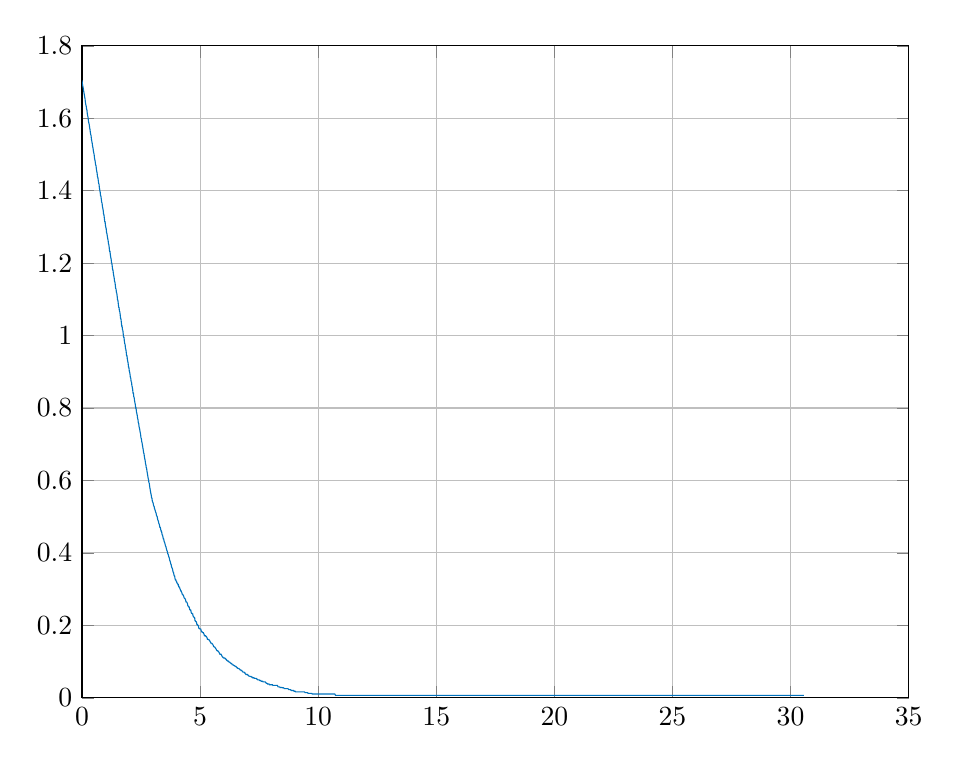
\begin{tikzpicture}

\begin{axis}[%
width=4.133in,
height=3.26in,
at={(0.693in,0.44in)},
scale only axis,
xmin=0,
xmax=35,
xmajorgrids,
ymin=0,
ymax=1.8,
ymajorgrids,
axis background/.style={fill=white}
]
\addplot [color=mycolor1,solid,forget plot]
  table[row sep=crcr]{%
0	1.70474009265444\\
0.0154305690000001	1.6946117787791\\
0.0316154210000001	1.68879128993211\\
0.0475025730000008	1.68489245235808\\
0.0634995650000013	1.67712459189975\\
0.0793436500000004	1.67129265971435\\
0.0954668219990004	1.66545477754443\\
0.111512549001001	1.6591803124907\\
0.127523247000001	1.65338290328949\\
0.143510858000001	1.64366438375055\\
0.159401588000001	1.63784466882344\\
0.175509877	1.63394591783211\\
0.191557036998	1.6261789820845\\
0.207529243001001	1.62228616784918\\
0.223483668000001	1.6125929369844\\
0.239521576999001	1.60633496802473\\
0.255498107000001	1.60243622975757\\
0.271699387001	1.5927183453039\\
0.287528178000001	1.58689929161325\\
0.303458137	1.58300074843834\\
0.319483212001001	1.57523473443522\\
0.335508217	1.56942235129128\\
0.351483460000001	1.56120823964905\\
0.367490379000001	1.55538962347341\\
0.38346966	1.55149084049952\\
0.399481891000001	1.54177371587573\\
0.415491071	1.53595546112013\\
0.431717979	1.53059160196791\\
0.447508191000001	1.52236905899086\\
0.463533842	1.5180391692981\\
0.479567789000001	1.51026345042084\\
0.495505515000001	1.5044455431419\\
0.511453015000001	1.50054700320433\\
0.527483541999001	1.48984540344975\\
0.543559237	1.48548386451496\\
0.559521370000001	1.4791888636504\\
0.575354941000002	1.47098802526299\\
0.591482278000001	1.46903617949439\\
0.607555908	1.45932030807742\\
0.623438195	1.45350301244915\\
0.639358087001001	1.44813503141055\\
0.655478291999001	1.4384189408551\\
0.671494563000001	1.43601955818042\\
0.687480925000001	1.42824464792829\\
0.703355088000001	1.42004581306627\\
0.719334530000001	1.41809377595275\\
0.735297800000001	1.40739045637248\\
0.751355283999	1.4010902111039\\
0.767349284	1.39673236254257\\
0.783269628	1.38701697911915\\
0.799299191999001	1.38507632471662\\
0.815494829	1.37686734815495\\
0.831622732000001	1.36811542401743\\
0.847536390000001	1.36567892057132\\
0.863582948001001	1.35596410589259\\
0.879453454	1.35162589423778\\
0.895460944	1.34578947462011\\
0.91146016	1.33607501504306\\
0.927463517000001	1.33320533550589\\
0.943432179000001	1.32493613651206\\
0.959437359000001	1.31473694507299\\
0.975395317	1.31473710358825\\
0.991649161	1.30456214950148\\
1.007405697	1.2987469959432\\
1.023472362	1.29484828248841\\
1.039481125001	1.28370924946386\\
1.055532892	1.28128361937447\\
1.071627123	1.27350997545483\\
1.0875471	1.2676951050852\\
1.10348633	1.26333512193061\\
1.11948266	1.25362174858199\\
1.135382545999	1.25068840553349\\
1.151327588	1.2424826983049\\
1.167292444	1.23228321210831\\
1.183299364	1.23228327318286\\
1.199317774	1.22257023512929\\
1.215301475	1.21629412165893\\
1.23147423	1.21140062789081\\
1.247531088	1.20168795327629\\
1.263568647	1.19926103294758\\
1.279450692	1.19105679377603\\
1.295494399	1.18134421778365\\
1.311483308	1.18088174865435\\
1.32750935	1.17116928594674\\
1.344395607	1.16435963744606\\
1.359816472999	1.15997334584973\\
1.375389227999	1.15026119875215\\
1.391453953	1.14789084731143\\
1.407517557	1.1401187272694\\
1.423466208	1.12994348945329\\
1.439365583	1.12894608161531\\
1.455392432	1.11923434569847\\
1.4715246	1.11680659130762\\
1.487480182999	1.10903452030747\\
1.503494238001	1.09889307475915\\
1.519488008	1.09695402397325\\
1.535394199	1.08771914270885\\
1.551287022999	1.07800795742058\\
1.567486639	1.07751907938506\\
1.583461640999	1.0678080913674\\
1.599503103	1.06586882099323\\
1.615451415	1.05766826001985\\
1.631458479	1.04745762028935\\
1.647294092	1.04649247993204\\
1.663392568	1.03678195870097\\
1.67961089	1.02658189696775\\
1.695419837	1.02658187074009\\
1.711454492	1.01687163241387\\
1.72746558	1.01493276647593\\
1.743402071999	1.00526610835494\\
1.759490676	0.995556173741503\\
1.775430362	0.995065934465773\\
1.791424403	0.985355986395056\\
1.80749287	0.97758247362802\\
1.823459781999	0.975646569730273\\
1.839425658999	0.964934360223328\\
1.855505213	0.962101238005707\\
1.871457918999	0.953839820260725\\
1.887361073001	0.944130416171333\\
1.90332065	0.94413041576904\\
1.919354309	0.934421629061999\\
1.935283389001	0.929524985980196\\
1.951364569	0.923708613095321\\
1.968718231001	0.913105329247332\\
1.983809665	0.912613699342077\\
1.999429547	0.902904736913392\\
2.01545803	0.899012235568544\\
2.031456805	0.893195774484707\\
2.047414383	0.884418108375302\\
2.063445958	0.882482250827322\\
2.079518656	0.872306058256905\\
2.095635885	0.871387344477817\\
2.111469967	0.861678382049132\\
2.127593970998	0.857785880704284\\
2.143650919	0.851467307945363\\
2.159486932999	0.841255895963062\\
2.175466397999	0.841255895963062\\
2.191479956999	0.831079703392645\\
2.207503934	0.82863420569127\\
2.223488743	0.820452027184872\\
2.239479997	0.814614867516652\\
2.255524577	0.809738503527487\\
2.271476932	0.800029541098802\\
2.287480522999	0.800029541098802\\
2.304132543	0.78936171862313\\
2.319771572	0.785469217278281\\
2.337643426	0.779652756194445\\
2.353029573001	0.771452655104413\\
2.368694999	0.768512148663227\\
2.384229211	0.758803186234542\\
2.399796232999	0.756849318438423\\
2.415717933	0.74813536375887\\
2.431489373999	0.744242862414021\\
2.447469041	0.738426401330185\\
2.463385255	0.732589241661965\\
2.47947872	0.727285793798967\\
2.495430696	0.717576831370282\\
2.51145325	0.715622963574163\\
2.527480001	0.707376239036342\\
2.54364869	0.703016507549761\\
2.559497389	0.697200046465925\\
2.575351587	0.690358325569004\\
2.591324038	0.68453265501242\\
2.607480706	0.676350476506022\\
2.623489199	0.674396608709903\\
2.639415501	0.666149884172082\\
2.655373342999	0.65984549436213\\
2.671348890999	0.655973691601665\\
2.687394764	0.64719602549226\\
2.703399127	0.64330630014816\\
2.719476916999	0.635551205515595\\
2.735660095	0.633170253845643\\
2.751481969999	0.624923529307822\\
2.767483743	0.61861913949787\\
2.783539903	0.612793468941286\\
2.799394817	0.605969670627999\\
2.815446854	0.6020799452839\\
2.831465845998	0.594324850651335\\
2.847504568	0.591943898981383\\
2.863577525	0.583697174443562\\
2.879406432	0.57739278463361\\
2.89551017	0.571065002401941\\
2.911500816	0.56474331576374\\
2.927393346	0.56085359041964\\
2.943476724	0.553098495787075\\
2.959569618	0.551144627990956\\
2.977335485	0.542897903453135\\
2.992548095998	0.540517169305024\\
3.007853441	0.538578535756294\\
3.023382701999	0.5322945867076\\
3.039386635	0.52933615768278\\
3.055335993	0.527397491102853\\
3.071335035	0.521581193231575\\
3.087317344	0.519627325435455\\
3.103335803	0.515744334405062\\
3.119379184999	0.511872531644597\\
3.13532033	0.509918663848477\\
3.151373799001	0.503608268538381\\
3.167348505	0.501672410990401\\
3.183317394	0.499718543194282\\
3.199339166	0.493472864931328\\
3.215348095	0.49006351915651\\
3.231318425999	0.488109651360391\\
3.247348600999	0.48229088883619\\
3.263451409	0.48035503128821\\
3.279287298999	0.476462529943361\\
3.295344699	0.470646714805256\\
3.311336538999	0.470646714805256\\
3.327486312	0.466262583555152\\
3.343907946	0.4604466947518\\
3.360054747	0.460446939980053\\
3.375608755	0.456554438635205\\
3.391468922	0.449734070594408\\
3.407491956999	0.449264121345858\\
3.423476956	0.444944536127177\\
3.439358475999	0.439128811365554\\
3.455379031	0.439128896939805\\
3.471325557999	0.433292555703488\\
3.487348674001	0.429420752943023\\
3.503408743	0.42746706072173\\
3.519335706	0.423093039545179\\
3.535486526	0.419221236784714\\
3.551505463	0.417267634682414\\
3.567372991	0.412883213964146\\
3.583509108	0.408508961650065\\
3.599491767	0.406083808560106\\
3.615496390999	0.402201581804241\\
3.631429252	0.397902695169943\\
3.647461529	0.395948934447029\\
3.663346075	0.39206679003769\\
3.679471052001	0.388194987277225\\
3.695479489999	0.385749687137632\\
3.711355246	0.379931679921535\\
3.727346429	0.377995822373555\\
3.743337718	0.374103321028707\\
3.759278162	0.369219756766323\\
3.775482047	0.367283899218343\\
3.791480571999	0.360975393060151\\
3.807374255	0.359039570095251\\
3.82333989	0.357103712547271\\
3.839336069999	0.35278412732859\\
3.855510203	0.346969274267229\\
3.871489715	0.346477644361974\\
3.887399569	0.340641962134616\\
3.903524937	0.336770463574814\\
3.919485965999	0.336770463574814\\
3.935566438	0.329930302761269\\
3.951380543999	0.32605889535557\\
3.968782614999	0.326058904315152\\
3.984097832001	0.322166402970304\\
3.999926472	0.321692622053704\\
4.015473163	0.317813849184494\\
4.031347413	0.315878184539633\\
4.04735214	0.31587836282973\\
4.063321975	0.311986303048865\\
4.079332458001	0.311986416784064\\
4.095285815	0.306172475526477\\
4.11131705	0.306172933222555\\
4.127350669	0.305253414576907\\
4.143317604	0.301361200007421\\
4.159332495	0.299418990822751\\
4.175360416	0.295548196968833\\
4.191360389001	0.295548234735275\\
4.207464108	0.292587112960259\\
4.2234899	0.290648864214857\\
4.239452659	0.286770844731883\\
4.255388828001	0.284835998571946\\
4.271493754	0.284836147023303\\
4.287467873	0.282882279227184\\
4.30338753	0.280944837440751\\
4.319419587	0.276590766215776\\
4.335468522	0.274655695021006\\
4.351491686	0.274655931305201\\
4.367476965999	0.272702444665964\\
4.383456057	0.270764679308974\\
4.399485567	0.26495235067969\\
4.415503602	0.264952920909066\\
4.431399602	0.264458523272355\\
4.447482240001	0.262504657497653\\
4.463425044	0.260140389073949\\
4.479307496	0.25432853421238\\
4.495411099	0.253316976534241\\
4.511483666999	0.251363503251914\\
4.527469304	0.25136359363976\\
4.543505599	0.249425907524886\\
4.559495434	0.243614706519443\\
4.575394779	0.243614991531186\\
4.591328071	0.241661123735066\\
4.607330590001	0.241661821335008\\
4.623522238	0.235369540924664\\
4.639512555	0.233434828380509\\
4.655413891	0.233435125672835\\
4.671387640999	0.231481756383861\\
4.687536373	0.231482005377405\\
4.703306805999	0.225668496334822\\
4.719304439999	0.223734561071014\\
4.735336461	0.223238204125737\\
4.751331743	0.221284400306203\\
4.767488307	0.221285107360124\\
4.783351104	0.213029778394622\\
4.799292805	0.212522084746233\\
4.815206005999	0.210141693150824\\
4.831340008999	0.210141809034182\\
4.8474735	0.208204898599737\\
4.86338512	0.202395118745234\\
4.879434118	0.20239554634534\\
4.895479544	0.200441678549221\\
4.911359434999	0.200442490100546\\
4.927347246	0.198505943614834\\
4.943306396999	0.192215693124293\\
4.959345649	0.192216054438702\\
4.976803863	0.190262828929709\\
4.992200052	0.190262828929709\\
5.007502134	0.190263199538075\\
5.023453778	0.190263529990605\\
5.040961929	0.186393038853988\\
5.056512198001	0.182518069892281\\
5.072064121	0.182518498614983\\
5.087864597	0.182019857256434\\
5.103495319	0.180066127774402\\
5.119481240001	0.180066565864961\\
5.135485428	0.18006700395552\\
5.151466318	0.177620377910384\\
5.167357079	0.175176336401499\\
5.183337166999	0.171301476502311\\
5.199285097	0.171301476502311\\
5.215337930999	0.171301720804295\\
5.231306778	0.17130213774702\\
5.247285189	0.169348269950901\\
5.263307928	0.169348523679992\\
5.279336737	0.167412576856905\\
5.295282271	0.165479019276537\\
5.311330635	0.161177295384989\\
5.327329776	0.161177611996647\\
5.343543081999	0.161177928608305\\
5.359484929	0.161178288620188\\
5.375467794	0.15922474693689\\
5.391353303	0.159225073049712\\
5.407297179	0.157289322183083\\
5.423374202	0.155356278787069\\
5.439282015999	0.15342341413812\\
5.455354038	0.151001991620567\\
5.471339032	0.151002426168109\\
5.487335428	0.151002860715651\\
5.503336389001	0.149049468995106\\
5.519351155	0.149049468995106\\
5.535359232	0.147114411997749\\
5.551342407	0.145181301285027\\
5.567319104999	0.142746314303769\\
5.583320543999	0.140805967776153\\
5.599305053	0.140805967776153\\
5.615337289	0.140806212801963\\
5.631359077	0.138339644313294\\
5.647343039	0.137826268884706\\
5.663303368	0.135890841487707\\
5.679343536998	0.133958135037398\\
5.695344347	0.132025607923012\\
5.711303719	0.130084527065573\\
5.727337423	0.130084851530045\\
5.743357131	0.130085175994518\\
5.759455463	0.128131669982316\\
5.775470715	0.128132004140155\\
5.791447111	0.126196831997703\\
5.807532117	0.124264629046207\\
5.8232788	0.12233240036906\\
5.839298744	0.120391401101686\\
5.855343984999	0.120391401101686\\
5.871294281	0.120391870260252\\
5.887295632	0.120392757156247\\
5.903301088	0.118011805486295\\
5.919299984	0.116077042136536\\
5.935341512	0.114145555874371\\
5.951331656999	0.112213163211808\\
5.969104218	0.112213739980786\\
5.98441277	0.110272859991204\\
5.999898252	0.109792956879823\\
6.015618862	0.10979354344484\\
6.031405817999	0.109794106229449\\
6.047438469	0.109794669014059\\
6.0633597	0.107841397578977\\
6.079330868	0.107841970174605\\
6.095422222999	0.10590756511019\\
6.111289713	0.105908259580253\\
6.127337217001	0.103470554359421\\
6.14387731	0.103471226963812\\
6.159478494	0.101539561369953\\
6.175456166999	0.101539561369953\\
6.191502109999	0.101540926318407\\
6.207651908	0.0995994933552509\\
6.223560259	0.0990825689457795\\
6.239519564	0.0985659783640573\\
6.255363243001	0.0985659783640573\\
6.271459975999	0.0966124969393898\\
6.287453284	0.0966128619893925\\
6.303459923	0.0946786029850759\\
6.319455446	0.0946790877756032\\
6.336234359999	0.0946794627111571\\
6.351781838	0.0927481668016046\\
6.367377529	0.0908169906762508\\
6.383495777	0.090817465989345\\
6.399363304001	0.090817941302439\\
6.415370083	0.0908184459514021\\
6.431323184999	0.0888774982457075\\
6.44732366	0.0888779835031688\\
6.463320600999	0.0888784980813273\\
6.479287044	0.086925125487022\\
6.495457343	0.0869256206888362\\
6.511713266	0.0869261451961736\\
6.527463283	0.0849919644749586\\
6.543358192999	0.0849929747672624\\
6.559558489999	0.0830616662431818\\
6.575375541999	0.0830622895230699\\
6.591395323	0.0811321926346187\\
6.607493098	0.0811321926346187\\
6.623389887999	0.0811328259025703\\
6.63960355	0.0811334417235197\\
6.655480508999	0.0791926245813133\\
6.671355209	0.079193267837308\\
6.687401100999	0.0772400258652541\\
6.703417842001	0.0772406516893198\\
6.719319362	0.0772413049333387\\
6.735243857999	0.0753081157663189\\
6.751289702	0.0753087515934814\\
6.767342034	0.0753095039045386\\
6.78336975	0.0733792044730204\\
6.7993681	0.0714490869667765\\
6.815492535	0.0714498493247226\\
6.831510724999	0.0710227654508897\\
6.847463657	0.0710242591603949\\
6.863251163	0.0710242591603949\\
6.87928786	0.0690835986020506\\
6.895295461	0.0690851124352601\\
6.911293154	0.0666507885541865\\
6.927493390999	0.066140004551051\\
6.943484349001	0.0642073032048585\\
6.959354378	0.0642080701832928\\
6.976952666	0.0642088206068472\\
6.992157069	0.0642095976470869\\
7.007445028	0.064210374687327\\
7.023286177	0.0622801009937279\\
7.039359789	0.0622808880957502\\
7.055379969	0.0603513678507361\\
7.071352653	0.0598285633154623\\
7.087376324999	0.0598294517947415\\
7.103301183	0.0593066356413365\\
7.119240311	0.059306872028734\\
7.13529481	0.0593074337343433\\
7.151299043	0.0593079954399531\\
7.167288152	0.0573668089744681\\
7.183339321001	0.0573668089744681\\
7.199356919	0.0573679526586073\\
7.215347576999	0.0554137129055237\\
7.231377317999	0.0554138953006484\\
7.247383685	0.0554150592576728\\
7.263372954	0.0554150592576728\\
7.27936498	0.0554152518225883\\
7.295351022	0.0534824649275367\\
7.311307331	0.0534830570424738\\
7.327490494	0.0534832597771735\\
7.345422892	0.0534838620285174\\
7.361082279	0.0534844642798618\\
7.376585807	0.05348467718434\\
7.392133149	0.0515554397432858\\
7.407511564	0.0515561437992782\\
7.423496087001	0.0515563668735286\\
7.439386494	0.0496273229641484\\
7.455452781	0.0496280372152949\\
7.471600463999	0.0496282704593105\\
7.487494703	0.0496282704593105\\
7.503485314999	0.0496297193518671\\
7.520069286998	0.0476885298024845\\
7.535694662	0.0476885298024845\\
7.551352234	0.0476899990852611\\
7.56750802	0.0476899990852611\\
7.583478916999	0.045735420880213\\
7.599414795	0.0457369105531642\\
7.615352112	0.0457369105531642\\
7.631346106001	0.0457371005699356\\
7.647275593	0.0457378556014763\\
7.663332187	0.043805231623028\\
7.67940285	0.0438054318690841\\
7.695382383999	0.0438061970956662\\
7.711322930999	0.0438069623222486\\
7.727328522	0.0438071727975835\\
7.743285197	0.0438079482191842\\
7.759319288	0.0438087236407849\\
7.775321038	0.0418798295084766\\
7.79127215	0.0418806151250719\\
7.807306253	0.0399524701816567\\
7.823393986	0.0399527011155292\\
7.839318478	0.0399527011155292\\
7.855482358	0.0380130441699331\\
7.871480206	0.0380130441699331\\
7.887504067999	0.0380132853330639\\
7.903501271	0.0380150818580349\\
7.919433775	0.0380150818580349\\
7.935582963999	0.0360599865570004\\
7.951558315	0.0360614375795691\\
7.969428698	0.0360623460957323\\
7.984679383	0.0360623460957323\\
8.000056319999	0.0360632648655459\\
8.015454328999	0.0360654696467673\\
8.03148425	0.0360654696467673\\
8.047459301	0.0360663986702032\\
8.063460136	0.0360686342137129\\
8.079537995999	0.0341354340096789\\
8.095516708	0.0341363732867086\\
8.111365036	0.0341387290837509\\
8.127454066	0.0341387290837509\\
8.143536350999	0.0341387290837509\\
8.159463775	0.034141211729787\\
8.175451126	0.0341420652324256\\
8.191453584	0.0341420652324256\\
8.207492856	0.0341445786551005\\
8.22347964	0.0341454424556007\\
8.239497223	0.0341454424556007\\
8.255326469	0.0341470166172\\
8.271400788	0.0341488607531746\\
8.287486313	0.0322206699447065\\
8.303486526999	0.0302935521532943\\
8.319484847	0.0302961239599855\\
8.335482048999	0.0302961239599855\\
8.351426511	0.0302972072892222\\
8.367451872	0.0302998099753877\\
8.383485371	0.028359134105721\\
8.399431833	0.0283602277471058\\
8.415425672	0.0283629457297809\\
8.43147359	0.0283629457297809\\
8.447573194	0.0283640496832804\\
8.463513168	0.0283667986043841\\
8.479404087	0.0278826161234529\\
8.49532001	0.0278826161234529\\
8.511238238	0.0278852459863907\\
8.527502710999	0.0278861715734993\\
8.543481841	0.027370556797071\\
8.559354845998	0.0254178709339881\\
8.575343324999	0.0254184695604784\\
8.591339133999	0.0254184695604784\\
8.607234771	0.0254200264684856\\
8.623349975	0.0254217702979758\\
8.639417361999	0.0254217702979758\\
8.655514099	0.0254229154995946\\
8.671362775	0.0254251123160467\\
8.687328851	0.0254251123160467\\
8.70331801	0.0254262678296089\\
8.719465923999	0.0248943552410548\\
8.735499308	0.024474094240551\\
8.751504692999	0.0225428914627397\\
8.767487683	0.0225452404727953\\
8.783420084	0.0225452404727953\\
8.79954608	0.0225452404727953\\
8.815464311	0.0225477197765296\\
8.831483191	0.0225484602850943\\
8.847424087	0.0206212926918212\\
8.863488325	0.0200887468900435\\
8.879403036	0.0200894977707193\\
8.895486842999	0.0200894977707193\\
8.9114795	0.0200917961415525\\
8.927392862	0.0200925573943165\\
8.943466868	0.0200925573943165\\
8.959891979999	0.0200940160638849\\
8.977568939	0.0181559994846774\\
8.992983631	0.0181559994846774\\
9.008387198	0.0181569741199825\\
9.023845621	0.0181592270947077\\
9.039595781	0.0162324333410329\\
9.055441449999	0.0162334183630537\\
9.071495946	0.0162357960467043\\
9.087382588	0.0162357960467043\\
9.103358001	0.0162367914554113\\
9.11934515	0.0162392002999676\\
9.135270646	0.0162392002999676\\
9.151343348	0.0162392002999676\\
9.167350367	0.0162418329878686\\
9.183343876	0.0162426461007197\\
9.199343503	0.0162426461007197\\
9.215460271001	0.01624530996406\\
9.231489406	0.0162461334488551\\
9.247516981	0.0162461334488551\\
9.263394022999	0.0162478019189705\\
9.279532207001	0.0162496623442676\\
9.295361303	0.0162496623442676\\
9.311351699999	0.0162506992994134\\
9.32739985	0.0162532327868501\\
9.345408709	0.0162532327868501\\
9.360571445	0.0162542801285273\\
9.375657838	0.0162568447764933\\
9.39146336	0.0162568447764933\\
9.407364383999	0.0162579025046703\\
9.423367337001	0.0162604983130876\\
9.439361996	0.0143051516196708\\
9.455472293999	0.0143051516196708\\
9.471478071	0.0143079713589707\\
9.487524294	0.0143088467031047\\
9.503354427	0.0143088467031047\\
9.519270604	0.0143116976173427\\
9.535457838	0.014312583333266\\
9.551473968	0.014312583333266\\
9.567409680999	0.0123848843640377\\
9.583331241999	0.0123858716496126\\
9.599350368	0.0123858716496126\\
9.61526995	0.0123869709234621\\
9.631333772	0.0123897826295805\\
9.647347331999	0.0123897826295805\\
9.663377216	0.0123908922897651\\
9.679626486	0.0123937352147332\\
9.695402406999	0.0123937352147332\\
9.711442847	0.0123948552612196\\
9.727377868	0.0123977294049513\\
9.743440914	0.0104722514840496\\
9.759267081999	0.0104734763448522\\
9.775337968	0.0104763817072593\\
9.791340340999	0.0104763817072593\\
9.807498503	0.0104763817072593\\
9.823503734	0.0104795141559677\\
9.839373587	0.0104805535939398\\
9.855283080001	0.0104805535939398\\
9.871485232	0.0104837172756056\\
9.887464849	0.0104847671439638\\
9.90354783	0.0104847671439638\\
9.919369710001	0.0104868004671437\\
9.935361415	0.0104890223572034\\
9.951383668999	0.0104890223572034\\
9.969009541999	0.0104902889973129\\
9.984499289	0.0104913597263461\\
9.999854155	0.0104913597263461\\
10.015495049001	0.0104913597263461\\
10.031711864	0.0104924408856686\\
10.047492099	0.0104924408856686\\
10.063335829	0.0104924408856686\\
10.079411418999	0.0104935324752466\\
10.095488567	0.0104935324752466\\
10.111468114	0.0104935324752466\\
10.127339436	0.0104935324752466\\
10.143334859	0.0104946344950476\\
10.159328407	0.0104946344950476\\
10.175352805999	0.0104946344950476\\
10.191395396	0.010495746945038\\
10.2074466	0.010495746945038\\
10.223357407	0.010495746945038\\
10.239373126	0.0104968698251831\\
10.255335227999	0.0104968698251831\\
10.27127932	0.0104968698251831\\
10.287353406	0.0104980031354496\\
10.305642984	0.0104980031354496\\
10.320729081	0.0104980031354496\\
10.336190833999	0.0104991468758022\\
10.351404074	0.0104991468758022\\
10.367471055	0.0104991468758022\\
10.383315686	0.0105003010462066\\
10.399480623	0.0105003010462066\\
10.415509557	0.0105003010462066\\
10.431591882	0.0105014656466276\\
10.447431467	0.0105014656466276\\
10.463482561	0.0105014656466276\\
10.479382092	0.0105014656466276\\
10.495347617	0.0105026406770299\\
10.51134313	0.0105026406770299\\
10.527464598	0.0105026406770299\\
10.54337541	0.0105038261373771\\
10.559460622	0.0105038261373771\\
10.575362793999	0.0105038261373771\\
10.591347262	0.0105050220276335\\
10.607482677	0.0105050220276335\\
10.623389775	0.0105050220276335\\
10.639489244	0.0105062283477624\\
10.655437494	0.0105062283477624\\
10.671260203	0.0105062283477624\\
10.687338422001	0.0105074450977276\\
10.703341953001	0.0105074450977276\\
10.719344536998	0.00855209840431104\\
10.735348325	0.00662494949993864\\
10.751496038	0.00662494949993864\\
10.767506824999	0.00662494949993864\\
10.7835207	0.00662494949993864\\
10.799487133	0.00662627971792862\\
10.815462981	0.00662627971792862\\
10.831461907	0.00662627971792862\\
10.847344555	0.00662762042438114\\
10.863303861	0.00662762042438114\\
10.879479623	0.00662762042438114\\
10.895382430999	0.00662897161925602\\
10.911452182	0.00662897161925602\\
10.927444944	0.00662897161925602\\
10.943469899	0.00663033330251106\\
10.959471937	0.00663033330251106\\
10.977062495	0.00663033330251106\\
10.992184178	0.00663033330251106\\
11.007399619	0.00663033330251106\\
11.023478430999	0.00663033330251106\\
11.039514319999	0.00663033330251106\\
11.055473826999	0.00663033330251106\\
11.071518852	0.00663033330251106\\
11.087424296	0.00663033330251106\\
11.103482757	0.00663033330251106\\
11.119607076999	0.00663033330251106\\
11.135483155	0.00663033330251106\\
11.151542047	0.00663033330251106\\
11.16745372	0.00663033330251106\\
11.183409132	0.00663033330251106\\
11.199289887	0.00663033330251106\\
11.215331883999	0.00663033330251106\\
11.231462072	0.00663033330251106\\
11.247467293	0.00663033330251106\\
11.263384098	0.00663033330251106\\
11.279448327	0.00663033330251106\\
11.295433561	0.00663033330251106\\
11.311457394	0.00663033330251106\\
11.327364180999	0.00663033330251106\\
11.343195228	0.00663033330251106\\
11.359347699999	0.00663033330251106\\
11.375413488	0.00663033330251106\\
11.391287923	0.00663033330251106\\
11.407348993	0.00663033330251106\\
11.423344126	0.00663033330251106\\
11.439275569	0.00663033330251106\\
11.455358325	0.00663033330251106\\
11.471402323001	0.00663033330251106\\
11.487366298	0.00663033330251106\\
11.503372656999	0.00663033330251106\\
11.519368116	0.00663033330251106\\
11.535309383	0.00663033330251106\\
11.551370274001	0.00663033330251106\\
11.567353644001	0.00663033330251106\\
11.583475317	0.00663033330251106\\
11.599483133	0.00663033330251106\\
11.615476321	0.00663033330251106\\
11.631367052	0.00663033330251106\\
11.647346003	0.00663033330251106\\
11.663469446001	0.00663033330251106\\
11.679616281999	0.00663033330251106\\
11.695352688	0.00663033330251106\\
11.711350305999	0.00663033330251106\\
11.727342054999	0.00663033330251106\\
11.743328022	0.00663033330251106\\
11.759354967	0.00663033330251106\\
11.775498951	0.00663033330251106\\
11.791516309	0.00663033330251106\\
11.807621065	0.00663033330251106\\
11.823481908001	0.00663033330251106\\
11.839460989	0.00663033330251106\\
11.855837	0.00663033330251106\\
11.87159046	0.00663033330251106\\
11.887506066	0.00663033330251106\\
11.903495315	0.00663033330251106\\
11.919487822	0.00663033330251106\\
11.935623402	0.00663033330251106\\
11.953017251	0.00663033330251106\\
11.968369236	0.00663033330251106\\
11.983799877	0.00663033330251106\\
11.99947496	0.00663033330251106\\
12.015500782	0.00663033330251106\\
12.031550828	0.00663033330251106\\
12.047400420999	0.00663033330251106\\
12.063452088	0.00663033330251106\\
12.079824318	0.00663033330251106\\
12.095482708	0.00663033330251106\\
12.1113521	0.00663033330251106\\
12.127479006	0.00663033330251106\\
12.143529352999	0.00663033330251106\\
12.159523494	0.00663033330251106\\
12.175495604	0.00663033330251106\\
12.191376191	0.00663033330251106\\
12.207672677	0.00663033330251106\\
12.223525411	0.00663033330251106\\
12.239461159	0.00663033330251106\\
12.255482897	0.00663033330251106\\
12.271636353	0.00663033330251106\\
12.287479842001	0.00663033330251106\\
12.30349326	0.00663033330251106\\
12.319361174001	0.00663033330251106\\
12.335400249	0.00663033330251106\\
12.35128604	0.00663033330251106\\
12.367487817	0.00663033330251106\\
12.383421615001	0.00663033330251106\\
12.399552448	0.00663033330251106\\
12.415491225	0.00663033330251106\\
12.43165759	0.00663033330251106\\
12.447690247	0.00663033330251106\\
12.463485121	0.00663033330251106\\
12.479362797	0.00663033330251106\\
12.495408048	0.00663033330251106\\
12.511345529	0.00663033330251106\\
12.52734641	0.00663033330251106\\
12.543313534	0.00663033330251106\\
12.559376941001	0.00663033330251106\\
12.575369963999	0.00663033330251106\\
12.591490595	0.00663033330251106\\
12.607496753	0.00663033330251106\\
12.623478559999	0.00663033330251106\\
12.639552065	0.00663033330251106\\
12.655353864	0.00663033330251106\\
12.671346055	0.00663033330251106\\
12.68740285	0.00663033330251106\\
12.703472042	0.00663033330251106\\
12.719462227999	0.00663033330251106\\
12.735499175	0.00663033330251106\\
12.751529036	0.00663033330251106\\
12.767509640999	0.00663033330251106\\
12.783433196	0.00663033330251106\\
12.799478237	0.00663033330251106\\
12.815474491999	0.00663033330251106\\
12.831451722999	0.00663033330251106\\
12.847471296	0.00663033330251106\\
12.863672465	0.00663033330251106\\
12.879403048	0.00663033330251106\\
12.895458527	0.00663033330251106\\
12.911608449999	0.00663033330251106\\
12.927524238001	0.00663033330251106\\
12.943467392999	0.00663033330251106\\
12.959350706	0.00663033330251106\\
12.975335871	0.00663033330251106\\
12.991354066	0.00663033330251106\\
13.007480155	0.00663033330251106\\
13.023522539	0.00663033330251106\\
13.039454258	0.00663033330251106\\
13.055325356	0.00663033330251106\\
13.071420036	0.00663033330251106\\
13.087432729	0.00663033330251106\\
13.103504621	0.00663033330251106\\
13.119372996	0.00663033330251106\\
13.135336467	0.00663033330251106\\
13.151328111	0.00663033330251106\\
13.167266495	0.00663033330251106\\
13.183328278	0.00663033330251106\\
13.199360078	0.00663033330251106\\
13.215306906	0.00663033330251106\\
13.231343142	0.00663033330251106\\
13.247354281	0.00663033330251106\\
13.263353151	0.00663033330251106\\
13.279311956	0.00663033330251106\\
13.295344834	0.00663033330251106\\
13.311335021	0.00663033330251106\\
13.327463559999	0.00663033330251106\\
13.343983933	0.00663033330251106\\
13.359411117	0.00663033330251106\\
13.375461115001	0.00663033330251106\\
13.391348317999	0.00663033330251106\\
13.409513242	0.00663033330251106\\
13.424621966	0.00663033330251106\\
13.440035014	0.00663033330251106\\
13.455516603	0.00663033330251106\\
13.471461069999	0.00663033330251106\\
13.487358055	0.00663033330251106\\
13.503335868	0.00663033330251106\\
13.519377701	0.00663033330251106\\
13.535400616999	0.00663033330251106\\
13.5514756	0.00663033330251106\\
13.567459938	0.00663033330251106\\
13.583632387001	0.00663033330251106\\
13.599342814	0.00663033330251106\\
13.615475934	0.00663033330251106\\
13.63148372	0.00663033330251106\\
13.647478581999	0.00663033330251106\\
13.663522074	0.00663033330251106\\
13.679460748	0.00663033330251106\\
13.695508054	0.00663033330251106\\
13.711452260999	0.00663033330251106\\
13.727525083999	0.00663033330251106\\
13.743282343	0.00663033330251106\\
13.759342748	0.00663033330251106\\
13.775324826	0.00663033330251106\\
13.791477649999	0.00663033330251106\\
13.807622377	0.00663033330251106\\
13.823488421	0.00663033330251106\\
13.839330677	0.00663033330251106\\
13.855307734	0.00663033330251106\\
13.871323277	0.00663033330251106\\
13.889482269001	0.00663033330251106\\
13.904487723	0.00663033330251106\\
13.919508698001	0.00663033330251106\\
13.935334466	0.00663033330251106\\
13.951328390999	0.00663033330251106\\
13.969436974	0.00663033330251106\\
13.984734039	0.00663033330251106\\
14.000026448	0.00663033330251106\\
14.015338087001	0.00663033330251106\\
14.031352833999	0.00663033330251106\\
14.047383998	0.00663033330251106\\
14.063306747	0.00663033330251106\\
14.079337599	0.00663033330251106\\
14.095329329	0.00663033330251106\\
14.111444488	0.00663033330251106\\
14.12743498	0.00663033330251106\\
14.143433364999	0.00663033330251106\\
14.159341766	0.00663033330251106\\
14.175497126	0.00663033330251106\\
14.191462566	0.00663033330251106\\
14.207371072	0.00663033330251106\\
14.223277435	0.00663033330251106\\
14.239351615001	0.00663033330251106\\
14.255350039	0.00663033330251106\\
14.271329411	0.00663033330251106\\
14.287334115001	0.00663033330251106\\
14.303471564999	0.00663033330251106\\
14.319459381	0.00663033330251106\\
14.335413967	0.00663033330251106\\
14.35134326	0.00663033330251106\\
14.36734872	0.00663033330251106\\
14.383351850999	0.00663033330251106\\
14.399319831	0.00663033330251106\\
14.415310373	0.00663033330251106\\
14.431340295	0.00663033330251106\\
14.447342062	0.00663033330251106\\
14.463279052001	0.00663033330251106\\
14.479335219	0.00663033330251106\\
14.495339767	0.00663033330251106\\
14.511337385	0.00663033330251106\\
14.527318199999	0.00663033330251106\\
14.543347039	0.00663033330251106\\
14.559280180999	0.00663033330251106\\
14.575160646001	0.00663033330251106\\
14.593166956999	0.00663033330251106\\
14.608009747	0.00663033330251106\\
14.623161830001	0.00663033330251106\\
14.641332319	0.00663033330251106\\
14.656511698	0.00663033330251106\\
14.671900625	0.00663033330251106\\
14.687487441999	0.00663033330251106\\
14.703367189	0.00663033330251106\\
14.719341559	0.00663033330251106\\
14.735436948001	0.00663033330251106\\
14.751302592001	0.00663033330251106\\
14.76730023	0.00663033330251106\\
14.783378932	0.00663033330251106\\
14.799260166999	0.00663033330251106\\
14.81531345	0.00663033330251106\\
14.831323607	0.00663033330251106\\
14.847331433	0.00663033330251106\\
14.863292032	0.00663033330251106\\
14.879292722	0.00663033330251106\\
14.89534791	0.00663033330251106\\
14.911334599001	0.00663033330251106\\
14.927331505	0.00663033330251106\\
14.943390046	0.00663033330251106\\
14.959421837	0.00663033330251106\\
14.976847406	0.00663033330251106\\
14.992114047	0.00663033330251106\\
15.007604189999	0.00663033330251106\\
15.023474003	0.00663033330251106\\
15.039500046	0.00663033330251106\\
15.055409699	0.00663033330251106\\
15.071464206	0.00663033330251106\\
15.087527879	0.00663033330251106\\
15.103536116	0.00663033330251106\\
15.119449618	0.00663033330251106\\
15.135563425	0.00663033330251106\\
15.151464308	0.00663033330251106\\
15.167347587	0.00663033330251106\\
15.183300763	0.00663033330251106\\
15.199534482999	0.00663033330251106\\
15.215463104	0.00663033330251106\\
15.251840607	0.00663033330251106\\
15.264675236999	0.00663033330251106\\
15.280908504	0.00663033330251106\\
15.296766255	0.00663033330251106\\
15.312729886	0.00663033330251106\\
15.328686313	0.00663033330251106\\
15.345018722	0.00663033330251106\\
15.360895932001	0.00663033330251106\\
15.377067028	0.00663033330251106\\
15.392951776001	0.00663033330251106\\
15.408914409	0.00663033330251106\\
15.424832377	0.00663033330251106\\
15.440668719	0.00663033330251106\\
15.456768333999	0.00663033330251106\\
15.472739225999	0.00663033330251106\\
15.488773130999	0.00663033330251106\\
15.504716951999	0.00663033330251106\\
15.520731744	0.00663033330251106\\
15.536692899999	0.00663033330251106\\
15.552696842001	0.00663033330251106\\
15.568697211	0.00663033330251106\\
15.58476601	0.00663033330251106\\
15.60077966	0.00663033330251106\\
15.61676053	0.00663033330251106\\
15.632806201	0.00663033330251106\\
15.648817961	0.00663033330251106\\
15.664797142999	0.00663033330251106\\
15.680774219	0.00663033330251106\\
15.696764701	0.00663033330251106\\
15.712759202	0.00663033330251106\\
15.728845802	0.00663033330251106\\
15.744728534	0.00663033330251106\\
15.760727265	0.00663033330251106\\
15.776760243	0.00663033330251106\\
15.792777434999	0.00663033330251106\\
15.80875396	0.00663033330251106\\
15.824876827	0.00663033330251106\\
15.840758456999	0.00663033330251106\\
15.856822411	0.00663033330251106\\
15.872918623	0.00663033330251106\\
15.888751789	0.00663033330251106\\
15.90502991	0.00663033330251106\\
15.920708696	0.00663033330251106\\
15.936855984999	0.00663033330251106\\
15.955454722	0.00663033330251106\\
15.969774158	0.00663033330251106\\
15.984892146001	0.00663033330251106\\
16.000688175	0.00663033330251106\\
16.016708147999	0.00663033330251106\\
16.032701885	0.00663033330251106\\
16.048878754	0.00663033330251106\\
16.064808241	0.00663033330251106\\
16.080766699	0.00663033330251106\\
16.096794071999	0.00663033330251106\\
16.112795268	0.00663033330251106\\
16.128792962	0.00663033330251106\\
16.144788085	0.00663033330251106\\
16.160881149	0.00663033330251106\\
16.176759607	0.00663033330251106\\
16.192835802999	0.00663033330251106\\
16.208793491999	0.00663033330251106\\
16.224696576999	0.00663033330251106\\
16.240773854999	0.00663033330251106\\
16.256819488999	0.00663033330251106\\
16.272718305	0.00663033330251106\\
16.288898565	0.00663033330251106\\
16.304813446	0.00663033330251106\\
16.320714396001	0.00663033330251106\\
16.336720777	0.00663033330251106\\
16.352791856	0.00663033330251106\\
16.368736205999	0.00663033330251106\\
16.384920997	0.00663033330251106\\
16.400979687	0.00663033330251106\\
16.41844863	0.00663033330251106\\
16.433664830999	0.00663033330251106\\
16.448776302999	0.00663033330251106\\
16.464700105	0.00663033330251106\\
16.480803901	0.00663033330251106\\
16.496788099001	0.00663033330251106\\
16.512735777	0.00663033330251106\\
16.528805178	0.00663033330251106\\
16.544848382	0.00663033330251106\\
16.560911015999	0.00663033330251106\\
16.576730729	0.00663033330251106\\
16.592730555999	0.00663033330251106\\
16.608854923999	0.00663033330251106\\
16.624636962	0.00663033330251106\\
16.640818954	0.00663033330251106\\
16.656673824	0.00663033330251106\\
16.672776146001	0.00663033330251106\\
16.688897147	0.00663033330251106\\
16.704878656	0.00663033330251106\\
16.720840018	0.00663033330251106\\
16.736609966	0.00663033330251106\\
16.754892006	0.00663033330251106\\
16.770090914	0.00663033330251106\\
16.785317294	0.00663033330251106\\
16.800741432	0.00663033330251106\\
16.81694584	0.00663033330251106\\
16.832747324	0.00663033330251106\\
16.848730587	0.00663033330251106\\
16.864843359	0.00663033330251106\\
16.880907651	0.00663033330251106\\
16.896780573001	0.00663033330251106\\
16.912839396	0.00663033330251106\\
16.928908713999	0.00663033330251106\\
16.944704297	0.00663033330251106\\
16.968676189999	0.00663033330251106\\
16.977392151999	0.00663033330251106\\
16.992623253	0.00663033330251106\\
17.008610395	0.00663033330251106\\
17.024722419	0.00663033330251106\\
17.040668472	0.00663033330251106\\
17.056732805999	0.00663033330251106\\
17.072843456	0.00663033330251106\\
17.088846416999	0.00663033330251106\\
17.104788019001	0.00663033330251106\\
17.120901814	0.00663033330251106\\
17.136742776	0.00663033330251106\\
17.152756017999	0.00663033330251106\\
17.168878436	0.00663033330251106\\
17.184987671	0.00663033330251106\\
17.200716594	0.00663033330251106\\
17.216768524	0.00663033330251106\\
17.232813723	0.00663033330251106\\
17.248838000999	0.00663033330251106\\
17.264848858	0.00663033330251106\\
17.280736904	0.00663033330251106\\
17.296892731	0.00663033330251106\\
17.312795904	0.00663033330251106\\
17.328823137	0.00663033330251106\\
17.346066324	0.00663033330251106\\
17.361325672	0.00663033330251106\\
17.377928425	0.00663033330251106\\
17.393232797	0.00663033330251106\\
17.408810757999	0.00663033330251106\\
17.42481169	0.00663033330251106\\
17.440806673	0.00663033330251106\\
17.456766344	0.00663033330251106\\
17.472805048999	0.00663033330251106\\
17.488812539	0.00663033330251106\\
17.504845019999	0.00663033330251106\\
17.520908323	0.00663033330251106\\
17.536848415	0.00663033330251106\\
17.552700234	0.00663033330251106\\
17.568744091	0.00663033330251106\\
17.584750338999	0.00663033330251106\\
17.600753264	0.00663033330251106\\
17.616764894	0.00663033330251106\\
17.632769548	0.00663033330251106\\
17.648730567	0.00663033330251106\\
17.664851224001	0.00663033330251106\\
17.680764922	0.00663033330251106\\
17.696731224	0.00663033330251106\\
17.712738298	0.00663033330251106\\
17.728726144	0.00663033330251106\\
17.744822827	0.00663033330251106\\
17.760765546	0.00663033330251106\\
17.776757972	0.00663033330251106\\
17.79278016	0.00663033330251106\\
17.808901979999	0.00663033330251106\\
17.824887846	0.00663033330251106\\
17.840889228	0.00663033330251106\\
17.856939845998	0.00663033330251106\\
17.872877022	0.00663033330251106\\
17.888739869	0.00663033330251106\\
17.904789305	0.00663033330251106\\
17.920876390999	0.00663033330251106\\
17.936900369	0.00663033330251106\\
17.95288861	0.00663033330251106\\
17.968912257001	0.00663033330251106\\
17.984774396001	0.00663033330251106\\
18.000903965	0.00663033330251106\\
18.016626597	0.00663033330251106\\
18.032598626	0.00663033330251106\\
18.048592515	0.00663033330251106\\
18.064777372	0.00663033330251106\\
18.080769377	0.00663033330251106\\
18.096758536	0.00663033330251106\\
18.112753277	0.00663033330251106\\
18.128778607999	0.00663033330251106\\
18.144877766	0.00663033330251106\\
18.160860295	0.00663033330251106\\
18.176771678	0.00663033330251106\\
18.19277571	0.00663033330251106\\
18.208898823001	0.00663033330251106\\
18.224890868	0.00663033330251106\\
18.24106685	0.00663033330251106\\
18.256651055999	0.00663033330251106\\
18.272674247	0.00663033330251106\\
18.288808039	0.00663033330251106\\
18.304975311	0.00663033330251106\\
18.320858349	0.00663033330251106\\
18.336811481	0.00663033330251106\\
18.352788050999	0.00663033330251106\\
18.370674635999	0.00663033330251106\\
18.385953705	0.00663033330251106\\
18.401288001	0.00663033330251106\\
18.416783105	0.00663033330251106\\
18.432758769	0.00663033330251106\\
18.448737623001	0.00663033330251106\\
18.464752936	0.00663033330251106\\
18.480740612	0.00663033330251106\\
18.496721291	0.00663033330251106\\
18.512731598	0.00663033330251106\\
18.528727126	0.00663033330251106\\
18.544737288	0.00663033330251106\\
18.560755717999	0.00663033330251106\\
18.576732518	0.00663033330251106\\
18.592732883	0.00663033330251106\\
18.608759225999	0.00663033330251106\\
18.624741785	0.00663033330251106\\
18.640730633	0.00663033330251106\\
18.656702272	0.00663033330251106\\
18.672723468	0.00663033330251106\\
18.688689373999	0.00663033330251106\\
18.704677717001	0.00663033330251106\\
18.720696788	0.00663033330251106\\
18.737023507	0.00663033330251106\\
18.752892719	0.00663033330251106\\
18.768897649	0.00663033330251106\\
18.784810529	0.00663033330251106\\
18.800755623999	0.00663033330251106\\
18.816752088999	0.00663033330251106\\
18.832793401	0.00663033330251106\\
18.848758555	0.00663033330251106\\
18.864715657	0.00663033330251106\\
18.880718571	0.00663033330251106\\
18.896741813	0.00663033330251106\\
18.912764942999	0.00663033330251106\\
18.928754607999	0.00663033330251106\\
18.944899319999	0.00663033330251106\\
18.966797521	0.00663033330251106\\
18.976876515	0.00663033330251106\\
18.993382966	0.00663033330251106\\
19.008948701	0.00663033330251106\\
19.02486776	0.00663033330251106\\
19.040889372	0.00663033330251106\\
19.056882415	0.00663033330251106\\
19.072947309999	0.00663033330251106\\
19.088917637	0.00663033330251106\\
19.104902461	0.00663033330251106\\
19.120620956	0.00663033330251106\\
19.138904930999	0.00663033330251106\\
19.154019022	0.00663033330251106\\
19.169050585	0.00663033330251106\\
19.184774628	0.00663033330251106\\
19.200815439	0.00663033330251106\\
19.216870151	0.00663033330251106\\
19.232808856001	0.00663033330251106\\
19.248904401001	0.00663033330251106\\
19.264769969	0.00663033330251106\\
19.280737329	0.00663033330251106\\
19.296663726	0.00663033330251106\\
19.312789133	0.00663033330251106\\
19.329188251	0.00663033330251106\\
19.345119228	0.00663033330251106\\
19.360921904	0.00663033330251106\\
19.376913749	0.00663033330251106\\
19.393341652	0.00663033330251106\\
19.408832335999	0.00663033330251106\\
19.42468754	0.00663033330251106\\
19.440766837	0.00663033330251106\\
19.456901430999	0.00663033330251106\\
19.472904774	0.00663033330251106\\
19.489031354001	0.00663033330251106\\
19.504985028	0.00663033330251106\\
19.520930858	0.00663033330251106\\
19.536988010999	0.00663033330251106\\
19.552794345998	0.00663033330251106\\
19.569280022999	0.00663033330251106\\
19.584755311	0.00663033330251106\\
19.60082395	0.00663033330251106\\
19.616801363	0.00663033330251106\\
19.632700876	0.00663033330251106\\
19.648810242	0.00663033330251106\\
19.664769107	0.00663033330251106\\
19.680759559001	0.00663033330251106\\
19.696763652	0.00663033330251106\\
19.712733777	0.00663033330251106\\
19.728747732	0.00663033330251106\\
19.74472732	0.00663033330251106\\
19.76074797	0.00663033330251106\\
19.776791963	0.00663033330251106\\
19.79281558	0.00663033330251106\\
19.808802208	0.00663033330251106\\
19.824808840999	0.00663033330251106\\
19.841015538	0.00663033330251106\\
19.856906735	0.00663033330251106\\
19.8729119	0.00663033330251106\\
19.889243234	0.00663033330251106\\
19.904869069	0.00663033330251106\\
19.920898719999	0.00663033330251106\\
19.936946998	0.00663033330251106\\
19.952895475	0.00663033330251106\\
19.968694168	0.00663033330251106\\
19.984697956999	0.00663033330251106\\
20.000778684999	0.00663033330251106\\
20.016870291	0.00663033330251106\\
20.032773489999	0.00663033330251106\\
20.048740824999	0.00663033330251106\\
20.064741338999	0.00663033330251106\\
20.08074909	0.00663033330251106\\
20.096711908999	0.00663033330251106\\
20.112681508	0.00663033330251106\\
20.128729751	0.00663033330251106\\
20.144753549001	0.00663033330251106\\
20.160781535	0.00663033330251106\\
20.176794929001	0.00663033330251106\\
20.192773694	0.00663033330251106\\
20.208775772	0.00663033330251106\\
20.224757885	0.00663033330251106\\
20.240733333	0.00663033330251106\\
20.256728896001	0.00663033330251106\\
20.272700862	0.00663033330251106\\
20.288732612	0.00663033330251106\\
20.304754535	0.00663033330251106\\
20.320769467	0.00663033330251106\\
20.33693032	0.00663033330251106\\
20.352909316	0.00663033330251106\\
20.368877687	0.00663033330251106\\
20.384902096	0.00663033330251106\\
20.400807751	0.00663033330251106\\
20.416720772	0.00663033330251106\\
20.432718911	0.00663033330251106\\
20.448721435	0.00663033330251106\\
20.464726856	0.00663033330251106\\
20.480886732	0.00663033330251106\\
20.496833970998	0.00663033330251106\\
20.512784712	0.00663033330251106\\
20.528726865001	0.00663033330251106\\
20.544753543	0.00663033330251106\\
20.56075285	0.00663033330251106\\
20.576925756	0.00663033330251106\\
20.59299045	0.00663033330251106\\
20.608906138	0.00663033330251106\\
20.624807743	0.00663033330251106\\
20.640794145	0.00663033330251106\\
20.65666706	0.00663033330251106\\
20.672809968	0.00663033330251106\\
20.688796872	0.00663033330251106\\
20.704676890999	0.00663033330251106\\
20.720912215999	0.00663033330251106\\
20.736822345	0.00663033330251106\\
20.75282517	0.00663033330251106\\
20.768736225999	0.00663033330251106\\
20.784757192	0.00663033330251106\\
20.800740786	0.00663033330251106\\
20.816725166999	0.00663033330251106\\
20.832735689	0.00663033330251106\\
20.848742107	0.00663033330251106\\
20.864722165001	0.00663033330251106\\
20.880884561	0.00663033330251106\\
20.896663989999	0.00663033330251106\\
20.912661156999	0.00663033330251106\\
20.928653915001	0.00663033330251106\\
20.944671982	0.00663033330251106\\
20.966147305999	0.00663033330251106\\
20.978236762	0.00663033330251106\\
20.993668286998	0.00663033330251106\\
21.009307467	0.00663033330251106\\
21.024887584	0.00663033330251106\\
21.040852578	0.00663033330251106\\
21.056765414	0.00663033330251106\\
21.072752749	0.00663033330251106\\
21.0887363	0.00663033330251106\\
21.104736713999	0.00663033330251106\\
21.120698491	0.00663033330251106\\
21.136695136	0.00663033330251106\\
21.152700748001	0.00663033330251106\\
21.168729962001	0.00663033330251106\\
21.184753529	0.00663033330251106\\
21.200726216	0.00663033330251106\\
21.216734232	0.00663033330251106\\
21.232869416999	0.00663033330251106\\
21.248868272999	0.00663033330251106\\
21.264748850999	0.00663033330251106\\
21.280739487	0.00663033330251106\\
21.29672333	0.00663033330251106\\
21.312914341	0.00663033330251106\\
21.331679521	0.00663033330251106\\
21.344834416	0.00663033330251106\\
21.360925031	0.00663033330251106\\
21.37667152	0.00663033330251106\\
21.392651752	0.00663033330251106\\
21.408771678	0.00663033330251106\\
21.424834944	0.00663033330251106\\
21.440845521999	0.00663033330251106\\
21.456833448	0.00663033330251106\\
21.47272896	0.00663033330251106\\
21.48890419	0.00663033330251106\\
21.50489607	0.00663033330251106\\
21.520908942	0.00663033330251106\\
21.536930841	0.00663033330251106\\
21.552911395	0.00663033330251106\\
21.568837800999	0.00663033330251106\\
21.584901529	0.00663033330251106\\
21.600879378	0.00663033330251106\\
21.616929034	0.00663033330251106\\
21.632996144	0.00663033330251106\\
21.648946094	0.00663033330251106\\
21.664660142999	0.00663033330251106\\
21.680900432	0.00663033330251106\\
21.696780163	0.00663033330251106\\
21.712851482999	0.00663033330251106\\
21.728732522	0.00663033330251106\\
21.744757382	0.00663033330251106\\
21.760779069	0.00663033330251106\\
21.776901930999	0.00663033330251106\\
21.792931456	0.00663033330251106\\
21.808845729999	0.00663033330251106\\
21.82499862	0.00663033330251106\\
21.840845201	0.00663033330251106\\
21.856704267	0.00663033330251106\\
21.872917025	0.00663033330251106\\
21.888907392	0.00663033330251106\\
21.904906057	0.00663033330251106\\
21.920896905	0.00663033330251106\\
21.937012726	0.00663033330251106\\
21.952930302001	0.00663033330251106\\
21.968703762	0.00663033330251106\\
21.984822865001	0.00663033330251106\\
22.000922394999	0.00663033330251106\\
22.016922949	0.00663033330251106\\
22.032917425	0.00663033330251106\\
22.048663163	0.00663033330251106\\
22.064874766	0.00663033330251106\\
22.080724543	0.00663033330251106\\
22.096894897999	0.00663033330251106\\
22.112893533001	0.00663033330251106\\
22.128897199999	0.00663033330251106\\
22.144828818	0.00663033330251106\\
22.160726204	0.00663033330251106\\
22.176728728	0.00663033330251106\\
22.192729674001	0.00663033330251106\\
22.208788800999	0.00663033330251106\\
22.224688402	0.00663033330251106\\
22.240769147999	0.00663033330251106\\
22.256946649	0.00663033330251106\\
22.272978015	0.00663033330251106\\
22.288910388	0.00663033330251106\\
22.304918159	0.00663033330251106\\
22.321041772999	0.00663033330251106\\
22.336726359	0.00663033330251106\\
22.352929996	0.00663033330251106\\
22.36890346	0.00663033330251106\\
22.384854171	0.00663033330251106\\
22.400706188	0.00663033330251106\\
22.41909205	0.00663033330251106\\
22.434379927	0.00663033330251106\\
22.449927297001	0.00663033330251106\\
22.465276755999	0.00663033330251106\\
22.480776167	0.00663033330251106\\
22.496964630999	0.00663033330251106\\
22.512783588999	0.00663033330251106\\
22.528725588	0.00663033330251106\\
22.544776132	0.00663033330251106\\
22.560737204	0.00663033330251106\\
22.576746929	0.00663033330251106\\
22.592741666	0.00663033330251106\\
22.608734693	0.00663033330251106\\
22.624704673	0.00663033330251106\\
22.640679696	0.00663033330251106\\
22.656688734	0.00663033330251106\\
22.672702995	0.00663033330251106\\
22.688731774	0.00663033330251106\\
22.704765534	0.00663033330251106\\
22.720878613	0.00663033330251106\\
22.736771053	0.00663033330251106\\
22.752707823	0.00663033330251106\\
22.768708087	0.00663033330251106\\
22.784714385	0.00663033330251106\\
22.800913845	0.00663033330251106\\
22.816929018	0.00663033330251106\\
22.832875088999	0.00663033330251106\\
22.84889402	0.00663033330251106\\
22.864893993001	0.00663033330251106\\
22.880901078	0.00663033330251106\\
22.896886519001	0.00663033330251106\\
22.912909213999	0.00663033330251106\\
22.928762336	0.00663033330251106\\
22.944832826	0.00663033330251106\\
22.965475873	0.00663033330251106\\
22.976726442	0.00663033330251106\\
22.992621949	0.00663033330251106\\
23.008812104	0.00663033330251106\\
23.024780633999	0.00663033330251106\\
23.040680257	0.00663033330251106\\
23.056849228	0.00663033330251106\\
23.072754757	0.00663033330251106\\
23.088758864999	0.00663033330251106\\
23.107265239	0.00663033330251106\\
23.122666184	0.00663033330251106\\
23.137906451	0.00663033330251106\\
23.152990814	0.00663033330251106\\
23.168858918	0.00663033330251106\\
23.184741566	0.00663033330251106\\
23.200785955	0.00663033330251106\\
23.216723326999	0.00663033330251106\\
23.232732245	0.00663033330251106\\
23.248726345	0.00663033330251106\\
23.264725552	0.00663033330251106\\
23.28073208	0.00663033330251106\\
23.296729131	0.00663033330251106\\
23.312695342999	0.00663033330251106\\
23.328829015	0.00663033330251106\\
23.344799206	0.00663033330251106\\
23.360756968	0.00663033330251106\\
23.376714614999	0.00663033330251106\\
23.392722845	0.00663033330251106\\
23.40890559	0.00663033330251106\\
23.424775028	0.00663033330251106\\
23.440670986	0.00663033330251106\\
23.456899336	0.00663033330251106\\
23.472722286	0.00663033330251106\\
23.488777752	0.00663033330251106\\
23.504868717	0.00663033330251106\\
23.520810303	0.00663033330251106\\
23.536867430999	0.00663033330251106\\
23.553017222999	0.00663033330251106\\
23.569021642	0.00663033330251106\\
23.584788968	0.00663033330251106\\
23.600905656	0.00663033330251106\\
23.616793555	0.00663033330251106\\
23.632760803	0.00663033330251106\\
23.648819491	0.00663033330251106\\
23.664725779	0.00663033330251106\\
23.680765315	0.00663033330251106\\
23.696734738999	0.00663033330251106\\
23.71279995	0.00663033330251106\\
23.72925293	0.00663033330251106\\
23.744781084	0.00663033330251106\\
23.760872088999	0.00663033330251106\\
23.776767625999	0.00663033330251106\\
23.792881979	0.00663033330251106\\
23.808849927	0.00663033330251106\\
23.824618801	0.00663033330251106\\
23.84073645	0.00663033330251106\\
23.856738949	0.00663033330251106\\
23.872773485	0.00663033330251106\\
23.888765035	0.00663033330251106\\
23.904787318	0.00663033330251106\\
23.920949047	0.00663033330251106\\
23.936903287	0.00663033330251106\\
23.952945215	0.00663033330251106\\
23.968851952	0.00663033330251106\\
23.984684147999	0.00663033330251106\\
24.000883887001	0.00663033330251106\\
24.016823507999	0.00663033330251106\\
24.032714102999	0.00663033330251106\\
24.048798624	0.00663033330251106\\
24.064618598	0.00663033330251106\\
24.083026651	0.00663033330251106\\
24.098139453001	0.00663033330251106\\
24.113679702	0.00663033330251106\\
24.128885903	0.00663033330251106\\
24.144855297	0.00663033330251106\\
24.160801224	0.00663033330251106\\
24.176812642	0.00663033330251106\\
24.192804672	0.00663033330251106\\
24.20881536	0.00663033330251106\\
24.224801904	0.00663033330251106\\
24.240744278	0.00663033330251106\\
24.259214022	0.00663033330251106\\
24.274582734999	0.00663033330251106\\
24.289717702	0.00663033330251106\\
24.304864102	0.00663033330251106\\
24.320796241	0.00663033330251106\\
24.336740858	0.00663033330251106\\
24.352771837	0.00663033330251106\\
24.36881556	0.00663033330251106\\
24.384824975	0.00663033330251106\\
24.400765859	0.00663033330251106\\
24.416799007	0.00663033330251106\\
24.432871751	0.00663033330251106\\
24.448754168	0.00663033330251106\\
24.46479576	0.00663033330251106\\
24.480800905	0.00663033330251106\\
24.496773321	0.00663033330251106\\
24.512734015	0.00663033330251106\\
24.529166689999	0.00663033330251106\\
24.54495927	0.00663033330251106\\
24.560821091	0.00663033330251106\\
24.576907643	0.00663033330251106\\
24.592807583999	0.00663033330251106\\
24.60880016	0.00663033330251106\\
24.624663257	0.00663033330251106\\
24.64085293	0.00663033330251106\\
24.656862271	0.00663033330251106\\
24.672847122	0.00663033330251106\\
24.688803705	0.00663033330251106\\
24.704885204	0.00663033330251106\\
24.720805838999	0.00663033330251106\\
24.736953255	0.00663033330251106\\
24.752935844	0.00663033330251106\\
24.768823529	0.00663033330251106\\
24.784747397999	0.00663033330251106\\
24.800641315	0.00663033330251106\\
24.818978680999	0.00663033330251106\\
24.834072512	0.00663033330251106\\
24.849189494	0.00663033330251106\\
24.864815206	0.00663033330251106\\
24.880742345998	0.00663033330251106\\
24.896755489999	0.00663033330251106\\
24.912764258999	0.00663033330251106\\
24.928738467999	0.00663033330251106\\
24.944741559	0.00663033330251106\\
24.965259592	0.00663033330251106\\
24.977148147	0.00663033330251106\\
24.992669871	0.00663033330251106\\
25.008756767	0.00663033330251106\\
25.024738574	0.00663033330251106\\
25.040762743	0.00663033330251106\\
25.056730322	0.00663033330251106\\
25.072691368	0.00663033330251106\\
25.088702149999	0.00663033330251106\\
25.104694807	0.00663033330251106\\
25.120682708	0.00663033330251106\\
25.13676386	0.00663033330251106\\
25.152766394999	0.00663033330251106\\
25.168799267	0.00663033330251106\\
25.184742903	0.00663033330251106\\
25.200728659	0.00663033330251106\\
25.216729234	0.00663033330251106\\
25.232750926	0.00663033330251106\\
25.24875555	0.00663033330251106\\
25.264745576	0.00663033330251106\\
25.280754785	0.00663033330251106\\
25.296732533	0.00663033330251106\\
25.312704433	0.00663033330251106\\
25.328750911	0.00663033330251106\\
25.344777920999	0.00663033330251106\\
25.360768348	0.00663033330251106\\
25.376911736	0.00663033330251106\\
25.392740095998	0.00663033330251106\\
25.409052614999	0.00663033330251106\\
25.42485817	0.00663033330251106\\
25.44090122	0.00663033330251106\\
25.45664717	0.00663033330251106\\
25.472832462	0.00663033330251106\\
25.48878064	0.00663033330251106\\
25.504840090999	0.00663033330251106\\
25.520931491	0.00663033330251106\\
25.536679028999	0.00663033330251106\\
25.552840482	0.00663033330251106\\
25.568991591	0.00663033330251106\\
25.584733516	0.00663033330251106\\
25.600907022999	0.00663033330251106\\
25.616897696	0.00663033330251106\\
25.632930262	0.00663033330251106\\
25.648805192	0.00663033330251106\\
25.664720399	0.00663033330251106\\
25.680760182	0.00663033330251106\\
25.696781916999	0.00663033330251106\\
25.712882857	0.00663033330251106\\
25.728785640999	0.00663033330251106\\
25.74487912	0.00663033330251106\\
25.760865930999	0.00663033330251106\\
25.776700699	0.00663033330251106\\
25.794949045	0.00663033330251106\\
25.810097014	0.00663033330251106\\
25.825434281	0.00663033330251106\\
25.840946703999	0.00663033330251106\\
25.856849939	0.00663033330251106\\
25.872717194	0.00663033330251106\\
25.88885251	0.00663033330251106\\
25.904839921	0.00663033330251106\\
25.921024831	0.00663033330251106\\
25.936744571	0.00663033330251106\\
25.952851708	0.00663033330251106\\
25.968760706	0.00663033330251106\\
25.984826475999	0.00663033330251106\\
26.000854144	0.00663033330251106\\
26.016747635	0.00663033330251106\\
26.032655944	0.00663033330251106\\
26.048632956999	0.00663033330251106\\
26.064608499	0.00663033330251106\\
26.080655213	0.00663033330251106\\
26.096687616	0.00663033330251106\\
26.112631587001	0.00663033330251106\\
26.128860455	0.00663033330251106\\
26.1449078	0.00663033330251106\\
26.160643180999	0.00663033330251106\\
26.176890633999	0.00663033330251106\\
26.192767318	0.00663033330251106\\
26.208844064	0.00663033330251106\\
26.227321406999	0.00663033330251106\\
26.242660135	0.00663033330251106\\
26.257980307	0.00663033330251106\\
26.273300878	0.00663033330251106\\
26.288768189	0.00663033330251106\\
26.304777679001	0.00663033330251106\\
26.320876577	0.00663033330251106\\
26.33682563	0.00663033330251106\\
26.352721077	0.00663033330251106\\
26.368805215	0.00663033330251106\\
26.384764823	0.00663033330251106\\
26.403202409	0.00663033330251106\\
26.418622914	0.00663033330251106\\
26.433958318	0.00663033330251106\\
26.449191282	0.00663033330251106\\
26.464773883999	0.00663033330251106\\
26.480967908001	0.00663033330251106\\
26.496791658001	0.00663033330251106\\
26.51281585	0.00663033330251106\\
26.528838474	0.00663033330251106\\
26.544822748	0.00663033330251106\\
26.560904608	0.00663033330251106\\
26.576807344	0.00663033330251106\\
26.594274062	0.00663033330251106\\
26.609468255	0.00663033330251106\\
26.624788272	0.00663033330251106\\
26.640901115001	0.00663033330251106\\
26.656785206	0.00663033330251106\\
26.672778833	0.00663033330251106\\
26.68884137	0.00663033330251106\\
26.704684637	0.00663033330251106\\
26.720830243001	0.00663033330251106\\
26.736927616999	0.00663033330251106\\
26.752672213	0.00663033330251106\\
26.768621634	0.00663033330251106\\
26.784665041	0.00663033330251106\\
26.800662676	0.00663033330251106\\
26.816748488	0.00663033330251106\\
26.832856956	0.00663033330251106\\
26.848995713999	0.00663033330251106\\
26.86486251	0.00663033330251106\\
26.880798114999	0.00663033330251106\\
26.896717691	0.00663033330251106\\
26.912806623999	0.00663033330251106\\
26.928688169	0.00663033330251106\\
26.944752193	0.00663033330251106\\
26.965450519	0.00663033330251106\\
26.977684264	0.00663033330251106\\
26.99332285	0.00663033330251106\\
27.008782145	0.00663033330251106\\
27.024857668	0.00663033330251106\\
27.040647772	0.00663033330251106\\
27.056764063	0.00663033330251106\\
27.072733206	0.00663033330251106\\
27.088836178	0.00663033330251106\\
27.104762018	0.00663033330251106\\
27.120740498	0.00663033330251106\\
27.13673135	0.00663033330251106\\
27.152745285	0.00663033330251106\\
27.168733031	0.00663033330251106\\
27.18475736	0.00663033330251106\\
27.200734436	0.00663033330251106\\
27.216734104	0.00663033330251106\\
27.232736247	0.00663033330251106\\
27.248726963999	0.00663033330251106\\
27.264736614999	0.00663033330251106\\
27.280730284	0.00663033330251106\\
27.296728879	0.00663033330251106\\
27.312710746	0.00663033330251106\\
27.329910208	0.00663033330251106\\
27.345714027	0.00663033330251106\\
27.361137788999	0.00663033330251106\\
27.376766647	0.00663033330251106\\
27.392730633	0.00663033330251106\\
27.408894884	0.00663033330251106\\
27.424908884	0.00663033330251106\\
27.440874679999	0.00663033330251106\\
27.45674093	0.00663033330251106\\
27.47291805	0.00663033330251106\\
27.489211539	0.00663033330251106\\
27.504779397	0.00663033330251106\\
27.520735769999	0.00663033330251106\\
27.536904817999	0.00663033330251106\\
27.553006528	0.00663033330251106\\
27.568798328	0.00663033330251106\\
27.584699479001	0.00663033330251106\\
27.60091839	0.00663033330251106\\
27.616947211	0.00663033330251106\\
27.632840689	0.00663033330251106\\
27.648707805999	0.00663033330251106\\
27.664759982	0.00663033330251106\\
27.680810229999	0.00663033330251106\\
27.696764008	0.00663033330251106\\
27.712729999	0.00663033330251106\\
27.728745458	0.00663033330251106\\
27.744766043	0.00663033330251106\\
27.760730326	0.00663033330251106\\
27.776727362	0.00663033330251106\\
27.792760987	0.00663033330251106\\
27.808731923999	0.00663033330251106\\
27.824760989	0.00663033330251106\\
27.840765206	0.00663033330251106\\
27.856942902	0.00663033330251106\\
27.872933515	0.00663033330251106\\
27.888861840999	0.00663033330251106\\
27.904921875	0.00663033330251106\\
27.920904324	0.00663033330251106\\
27.936843463999	0.00663033330251106\\
27.953022052	0.00663033330251106\\
27.968824635999	0.00663033330251106\\
27.984848927	0.00663033330251106\\
28.000781942999	0.00663033330251106\\
28.016721951	0.00663033330251106\\
28.03274006	0.00663033330251106\\
28.048731264001	0.00663033330251106\\
28.064788416	0.00663033330251106\\
28.08124296	0.00663033330251106\\
28.096857258999	0.00663033330251106\\
28.11282025	0.00663033330251106\\
28.129037966	0.00663033330251106\\
28.14478867	0.00663033330251106\\
28.160811649	0.00663033330251106\\
28.176706102	0.00663033330251106\\
28.193004475999	0.00663033330251106\\
28.208792094	0.00663033330251106\\
28.224888087	0.00663033330251106\\
28.240730522999	0.00663033330251106\\
28.256835454	0.00663033330251106\\
28.272820007	0.00663033330251106\\
28.288766383	0.00663033330251106\\
28.304884696	0.00663033330251106\\
28.320821247	0.00663033330251106\\
28.336904823	0.00663033330251106\\
28.35271568	0.00663033330251106\\
28.368928243	0.00663033330251106\\
28.384832274	0.00663033330251106\\
28.400770614	0.00663033330251106\\
28.416823758	0.00663033330251106\\
28.432780343	0.00663033330251106\\
28.448809415	0.00663033330251106\\
28.464773457001	0.00663033330251106\\
28.480703177999	0.00663033330251106\\
28.496813455001	0.00663033330251106\\
28.512774274	0.00663033330251106\\
28.528735599	0.00663033330251106\\
28.544859508999	0.00663033330251106\\
28.560755795999	0.00663033330251106\\
28.576752416	0.00663033330251106\\
28.592982631	0.00663033330251106\\
28.608827915001	0.00663033330251106\\
28.624810164	0.00663033330251106\\
28.640636333999	0.00663033330251106\\
28.656671337	0.00663033330251106\\
28.672829878998	0.00663033330251106\\
28.68881976	0.00663033330251106\\
28.704744993999	0.00663033330251106\\
28.720868666999	0.00663033330251106\\
28.737172338	0.00663033330251106\\
28.753007947	0.00663033330251106\\
28.768961779	0.00663033330251106\\
28.784994546	0.00663033330251106\\
28.800898472	0.00663033330251106\\
28.819343316	0.00663033330251106\\
28.834524389001	0.00663033330251106\\
28.849631594	0.00663033330251106\\
28.864906792	0.00663033330251106\\
28.880805638	0.00663033330251106\\
28.896742592	0.00663033330251106\\
28.912901508	0.00663033330251106\\
28.928863369	0.00663033330251106\\
28.945573808	0.00663033330251106\\
28.966548055999	0.00663033330251106\\
28.978543588	0.00663033330251106\\
28.993816713999	0.00663033330251106\\
29.008951131	0.00663033330251106\\
29.024730338	0.00663033330251106\\
29.040703626	0.00663033330251106\\
29.056739566	0.00663033330251106\\
29.072766239999	0.00663033330251106\\
29.088738631	0.00663033330251106\\
29.104738885	0.00663033330251106\\
29.120770048999	0.00663033330251106\\
29.136751786	0.00663033330251106\\
29.15277648	0.00663033330251106\\
29.168757088999	0.00663033330251106\\
29.184778878	0.00663033330251106\\
29.200770361999	0.00663033330251106\\
29.21675483	0.00663033330251106\\
29.232765026	0.00663033330251106\\
29.24873241	0.00663033330251106\\
29.264738192	0.00663033330251106\\
29.280727211	0.00663033330251106\\
29.296727605	0.00663033330251106\\
29.312728104	0.00663033330251106\\
29.328772293	0.00663033330251106\\
29.344955381	0.00663033330251106\\
29.360884329	0.00663033330251106\\
29.376904939	0.00663033330251106\\
29.393004197	0.00663033330251106\\
29.408919467999	0.00663033330251106\\
29.424806571	0.00663033330251106\\
29.440845793	0.00663033330251106\\
29.456766050999	0.00663033330251106\\
29.472797345	0.00663033330251106\\
29.488761593	0.00663033330251106\\
29.504767119	0.00663033330251106\\
29.520722496	0.00663033330251106\\
29.536731939999	0.00663033330251106\\
29.552757842999	0.00663033330251106\\
29.568908352	0.00663033330251106\\
29.584935121	0.00663033330251106\\
29.600763245	0.00663033330251106\\
29.616759054001	0.00663033330251106\\
29.632706883999	0.00663033330251106\\
29.648740338999	0.00663033330251106\\
29.664742953	0.00663033330251106\\
29.680904357	0.00663033330251106\\
29.696898908	0.00663033330251106\\
29.712798438	0.00663033330251106\\
29.728802741999	0.00663033330251106\\
29.744733864	0.00663033330251106\\
29.76072418	0.00663033330251106\\
29.776732408	0.00663033330251106\\
29.792727565	0.00663033330251106\\
29.808762477	0.00663033330251106\\
29.824877456999	0.00663033330251106\\
29.840618040001	0.00663033330251106\\
29.85660923	0.00663033330251106\\
29.872639122	0.00663033330251106\\
29.888628892	0.00663033330251106\\
29.904695807	0.00663033330251106\\
29.920695184	0.00663033330251106\\
29.93670971	0.00663033330251106\\
29.952721661	0.00663033330251106\\
29.968729587001	0.00663033330251106\\
29.984769760999	0.00663033330251106\\
30.000791559	0.00663033330251106\\
30.016770946	0.00663033330251106\\
30.032747791999	0.00663033330251106\\
30.048706336	0.00663033330251106\\
30.064701423	0.00663033330251106\\
30.080773490001	0.00663033330251106\\
30.096756239999	0.00663033330251106\\
30.112706841	0.00663033330251106\\
30.128756637	0.00663033330251106\\
30.144741396	0.00663033330251106\\
30.160813227	0.00663033330251106\\
30.176758031	0.00663033330251106\\
30.192732045	0.00663033330251106\\
30.208762592	0.00663033330251106\\
30.224743543	0.00663033330251106\\
30.240739305999	0.00663033330251106\\
30.256736453	0.00663033330251106\\
30.272722174001	0.00663033330251106\\
30.288733178	0.00663033330251106\\
30.305080779	0.00663033330251106\\
30.320752012	0.00663033330251106\\
30.336775307999	0.00663033330251106\\
30.352625492	0.00663033330251106\\
30.368734567999	0.00663033330251106\\
30.384757207001	0.00663033330251106\\
30.400753087	0.00663033330251106\\
30.416714904	0.00663033330251106\\
30.432730227	0.00663033330251106\\
30.448733517	0.00663033330251106\\
30.464906603	0.00663033330251106\\
30.480905404	0.00663033330251106\\
30.496895981	0.00663033330251106\\
30.519118732	0.00663033330251106\\
30.528674007	0.00663033330251106\\
30.544708877	0.00663033330251106\\
30.560633998	0.00663033330251106\\
};
\end{axis}
\end{tikzpicture}%}
      \caption{The error in displacement of the robot over time for
        $(K_{\Psi}^R, K_{\omega}^T) \equiv (0.5 K_{\Psi, max}^R, 0.2 K_{\omega, max}^T)$}
      \label{fig:19_10_distance}
    \end{figure}
  \end{minipage}
  \hfill
  \begin{minipage}{0.45\linewidth}
    \begin{figure}[H]
      \scalebox{0.6}{% This file was created by matlab2tikz.
%
%The latest updates can be retrieved from
%  http://www.mathworks.com/matlabcentral/fileexchange/22022-matlab2tikz-matlab2tikz
%where you can also make suggestions and rate matlab2tikz.
%
\definecolor{mycolor1}{rgb}{0.00000,0.44700,0.74100}%
%
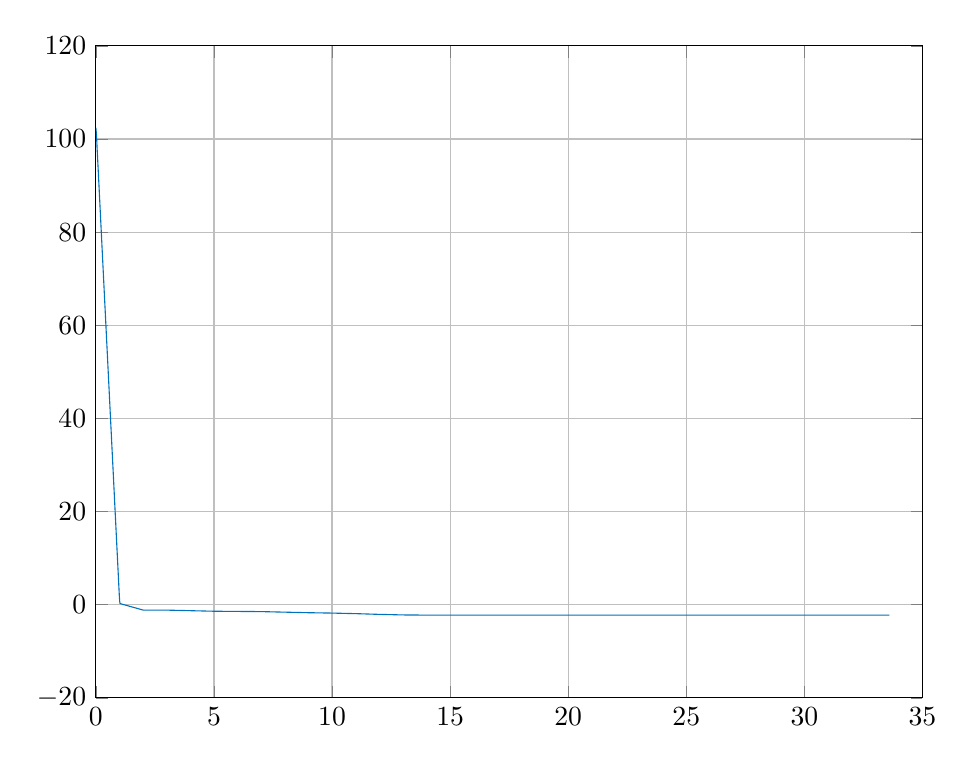
\begin{tikzpicture}

\begin{axis}[%
width=4.133in,
height=3.26in,
at={(0.693in,0.44in)},
scale only axis,
xmin=0,
xmax=35,
xmajorgrids,
ymin=-20,
ymax=120,
ymajorgrids,
axis background/.style={fill=white}
]
\addplot [color=mycolor1,solid,forget plot]
  table[row sep=crcr]{%
0	102.4204\\
0.0273090899999998	100.7844\\
0.036050307	99.9064\\
0.048114915	98.3984\\
0.0639762640000004	96.8264\\
0.0800080649990002	95.2244\\
0.0960188780000005	93.6204\\
0.111992261	91.9844\\
0.127933904	90.3544\\
0.144043623999001	88.7224\\
0.160088124001	87.0904\\
0.176044062	85.4704\\
0.192030885	83.8164\\
0.208235899	82.1744\\
0.224042703999001	80.5424\\
0.240142654	78.9044\\
0.256043894	77.2764\\
0.271862767999	75.6344\\
0.288037456	74.0024\\
0.304077224	72.3584\\
0.32005167	70.7204\\
0.336032846001	69.0904\\
0.352030684	67.4404\\
0.367915742000001	65.8144\\
0.384042802999	64.1564\\
0.399851736	62.5404\\
0.415904752	60.9044\\
0.431912634000001	59.2424\\
0.447895804	57.6224\\
0.463869978	55.9864\\
0.480020242000001	54.3824\\
0.496009146000001	52.7284\\
0.512131988	51.0884\\
0.528034019	49.4544\\
0.544014547999	47.8124\\
0.559968618	46.1884\\
0.5758931	44.5444\\
0.591885787	42.9004\\
0.607822441	41.2684\\
0.623880201	39.6244\\
0.639855944	38.0064\\
0.655825383	36.3784\\
0.671853134	34.7204\\
0.687883793	33.0824\\
0.703884011	31.4504\\
0.719900346999	29.8164\\
0.736353106000001	28.1744\\
0.752054757999	26.5384\\
0.768040424	24.9084\\
0.784242811	23.2624\\
0.800038502	21.6144\\
0.816035463	19.9884\\
0.831902455	18.3584\\
0.848005232	16.7304\\
0.863938337999	15.0864\\
0.879900545998	13.4664\\
0.895910738	11.8224\\
0.911903419	10.1884\\
0.928005559	8.5664\\
0.944046530001	6.9324\\
0.960008512998	5.2684\\
0.975908379000001	3.6384\\
0.991917354	2.02239999999999\\
1.009571379	0.63839999999999\\
1.025022179	0.230399999999989\\
1.040547476	0.210400000000007\\
1.056032989	0.184399999999997\\
1.071880086	0.164400000000001\\
1.087855243	0.1404\\
1.104027807	0.11839999999998\\
1.120077127	0.0963999999999885\\
1.135899627	0.0723999999999876\\
1.152042375	0.0503999999999962\\
1.168041306001	0.0263999999999953\\
1.184040643	0.00639999999998508\\
1.200124672	-0.0175999999999874\\
1.216072252	-0.0416000000000167\\
1.232057692	-0.0655999999999892\\
1.248060721999	-0.0875999999999948\\
1.264018474999	-0.111600000000024\\
1.280051468	-0.131600000000006\\
1.296212106	-0.155600000000007\\
1.312046207999	-0.177600000000012\\
1.328028936999	-0.201600000000013\\
1.344199928	-0.221600000000009\\
1.360041302	-0.245599999999996\\
1.375994088	-0.269600000000011\\
1.391974588	-0.291600000000017\\
1.408035448999	-0.315599999999989\\
1.423915078999	-0.33959999999999\\
1.439887951	-0.3596\\
1.456007358	-0.383600000000001\\
1.472010681	-0.407600000000031\\
1.488036017	-0.429600000000008\\
1.504030428	-0.453600000000009\\
1.520021075	-0.473600000000005\\
1.536043148001	-0.497600000000006\\
1.552038969	-0.521600000000007\\
1.56828979	-0.543599999999998\\
1.584053051	-0.567600000000013\\
1.599977453	-0.58959999999999\\
1.615951059	-0.611599999999996\\
1.632004797	-0.635599999999997\\
1.647974566	-0.657600000000002\\
1.663880737	-0.681600000000003\\
1.679849314999	-0.701600000000013\\
1.695835787	-0.725600000000014\\
1.711834402	-0.747600000000006\\
1.727844438	-0.771600000000007\\
1.743850365	-0.795600000000007\\
1.75983778	-0.815599999999989\\
1.775844859999	-0.83959999999999\\
1.791838554	-0.861600000000024\\
1.807895837	-0.885599999999997\\
1.823860405001	-0.909599999999998\\
1.839858884999	-0.929600000000008\\
1.856036957	-0.953600000000009\\
1.872042919	-0.97760000000001\\
1.887919438	-0.999600000000015\\
1.903945277	-1.02360000000002\\
1.920070497	-1.04760000000002\\
1.936056769	-1.0676\\
1.952046057999	-1.09160000000001\\
1.968047991	-1.1156\\
1.984012243	-1.13759999999999\\
2.000033931	-1.16160000000002\\
2.017683217	-1.17160000000001\\
2.032940788	-1.17360000000001\\
2.048423599	-1.17360000000001\\
2.063923925	-1.17160000000001\\
2.079919619	-1.17360000000001\\
2.0959255	-1.17360000000001\\
2.111947719	-1.17160000000001\\
2.127884950001	-1.17160000000001\\
2.143845023	-1.17360000000001\\
2.159920512	-1.17160000000001\\
2.175954288	-1.17160000000001\\
2.191805359	-1.17360000000001\\
2.207972581	-1.17160000000001\\
2.223942611	-1.17160000000001\\
2.239906445	-1.17360000000001\\
2.255979028999	-1.17360000000001\\
2.271915019	-1.17160000000001\\
2.287887882999	-1.17360000000001\\
2.303936604998	-1.17360000000001\\
2.319943754	-1.17160000000001\\
2.335867552999	-1.17360000000001\\
2.352043838	-1.17360000000001\\
2.368039856999	-1.17160000000001\\
2.384049809	-1.17360000000001\\
2.400036394	-1.17360000000001\\
2.416121363	-1.17160000000001\\
2.432005844	-1.17160000000001\\
2.447889939999	-1.17360000000001\\
2.464029023	-1.17160000000001\\
2.480077572	-1.17160000000001\\
2.496030729	-1.17360000000001\\
2.51207603	-1.17160000000001\\
2.528034844999	-1.17160000000001\\
2.544038537	-1.17360000000001\\
2.560325079	-1.17360000000001\\
2.575819447	-1.17160000000001\\
2.591902744	-1.17360000000001\\
2.60791909	-1.17360000000001\\
2.623950929	-1.17160000000001\\
2.640056011	-1.17360000000001\\
2.656086506	-1.17360000000001\\
2.672183412	-1.17160000000001\\
2.688079474999	-1.17360000000001\\
2.704027416	-1.17360000000001\\
2.720016240001	-1.17160000000001\\
2.736044641001	-1.17360000000001\\
2.752034531999	-1.17360000000001\\
2.768045164	-1.17160000000001\\
2.784032534	-1.17360000000001\\
2.799944843	-1.17360000000001\\
2.815937509	-1.17160000000001\\
2.832082297	-1.17160000000001\\
2.848070123	-1.17360000000001\\
2.864143437	-1.17160000000001\\
2.880195017	-1.17160000000001\\
2.896039432999	-1.17360000000001\\
2.912053502999	-1.17360000000001\\
2.927925527	-1.17160000000001\\
2.943921426	-1.17360000000001\\
2.959907753	-1.17360000000001\\
2.975856545998	-1.17160000000001\\
2.991993554	-1.17360000000001\\
3.009737530001	-1.17360000000001\\
3.025039948	-1.17360000000001\\
3.040553884	-1.17960000000001\\
3.055984453	-1.17960000000001\\
3.072169305	-1.17960000000001\\
3.088056457	-1.1836\\
3.104053449	-1.18559999999999\\
3.119897534	-1.18559999999999\\
3.136020705999	-1.1876\\
3.152066433001	-1.19160000000002\\
3.168077131	-1.19160000000002\\
3.184064742	-1.19360000000002\\
3.199955472	-1.19760000000001\\
3.216063761	-1.19760000000001\\
3.232110920998	-1.1996\\
3.248083127001	-1.20360000000001\\
3.264037552	-1.2056\\
3.280075460999	-1.20360000000001\\
3.296051991	-1.20959999999999\\
3.312253271001	-1.20959999999999\\
3.328082062	-1.20959999999999\\
3.344012021	-1.21559999999999\\
3.360037096001	-1.21559999999999\\
3.376062101	-1.21559999999999\\
3.392037344	-1.22160000000001\\
3.408044263	-1.22160000000001\\
3.424023544	-1.22160000000001\\
3.440035775	-1.2236\\
3.456044955	-1.22760000000001\\
3.472271863	-1.22760000000001\\
3.488062075	-1.2296\\
3.504087726	-1.2336\\
3.520121673	-1.2336\\
3.536059399	-1.23560000000001\\
3.552006899	-1.2396\\
3.568037425999	-1.24160000000002\\
3.584113121	-1.23960000000002\\
3.600075254	-1.24560000000001\\
3.615908825	-1.24560000000001\\
3.632036162	-1.24560000000001\\
3.648109792	-1.25160000000001\\
3.663992079	-1.25160000000001\\
3.679911971001	-1.25160000000001\\
3.696032175999	-1.2576\\
3.712048447	-1.2576\\
3.728034809	-1.2576\\
3.743908972	-1.2636\\
3.759888414	-1.2636\\
3.775851684	-1.2636\\
3.791909167999	-1.26559999999999\\
3.807903168	-1.26960000000001\\
3.823823512	-1.26960000000001\\
3.839853075999	-1.27160000000001\\
3.856048713	-1.27560000000001\\
3.872176616	-1.27560000000001\\
3.888090274	-1.27760000000001\\
3.904136832001	-1.2816\\
3.920007338	-1.28360000000001\\
3.936014828	-1.2816\\
3.952014044	-1.2876\\
3.968017401	-1.2876\\
3.983986063	-1.2876\\
3.999991243	-1.2936\\
4.015949201	-1.2936\\
4.032203045	-1.29559999999999\\
4.047959581	-1.29960000000001\\
4.064026246	-1.29960000000001\\
4.080035009001	-1.30160000000001\\
4.096086776	-1.3036\\
4.112181007	-1.3056\\
4.128100984	-1.30760000000001\\
4.144040214	-1.3096\\
4.160036544	-1.3116\\
4.175936429999	-1.31359999999999\\
4.191881472	-1.31560000000002\\
4.207846328	-1.31760000000001\\
4.223853248	-1.31960000000001\\
4.239871658	-1.31960000000001\\
4.255855359	-1.32360000000001\\
4.272028114	-1.32360000000001\\
4.288084972	-1.32560000000001\\
4.304122531	-1.3296\\
4.320004576	-1.3296\\
4.336048283	-1.33160000000001\\
4.352037192	-1.3356\\
4.368063234	-1.3356\\
4.384949491	-1.33759999999999\\
4.400370356999	-1.3416\\
4.415943111999	-1.3416\\
4.432007837	-1.3436\\
4.448071441	-1.34559999999999\\
4.464020092	-1.34759999999999\\
4.479919467	-1.34959999999998\\
4.495946316	-1.3516\\
4.512078484	-1.3536\\
4.528034066999	-1.35560000000001\\
4.544048122001	-1.35760000000001\\
4.560041892	-1.3596\\
4.575948083	-1.3616\\
4.591840906999	-1.3616\\
4.608040523	-1.3656\\
4.624015524999	-1.3656\\
4.640056987	-1.3676\\
4.656005299	-1.37160000000002\\
4.672012363	-1.37160000000002\\
4.687847976	-1.37360000000001\\
4.703946452	-1.3776\\
4.720164774	-1.3776\\
4.735973721	-1.37960000000001\\
4.752008376	-1.38160000000001\\
4.768019464	-1.3836\\
4.783955955999	-1.3856\\
4.80004456	-1.38759999999999\\
4.815984246	-1.3896\\
4.831978287	-1.39160000000001\\
4.848046754	-1.39360000000002\\
4.864013665999	-1.39560000000002\\
4.879979542999	-1.39760000000001\\
4.896059097	-1.39760000000001\\
4.912011802999	-1.4016\\
4.927914957001	-1.4016\\
4.943874534	-1.40360000000001\\
4.959908193	-1.4076\\
4.975837273001	-1.4076\\
4.991918453	-1.4096\\
5.009272115001	-1.41159999999999\\
5.024363549	-1.41159999999999\\
5.039983431	-1.41159999999999\\
5.056011914	-1.4136\\
5.072010689	-1.4136\\
5.087968267	-1.4136\\
5.103999842	-1.4136\\
5.12007254	-1.41560000000001\\
5.136189769	-1.41560000000001\\
5.152023851	-1.41560000000001\\
5.168147854998	-1.41760000000002\\
5.184204803	-1.41760000000002\\
5.200040816999	-1.41760000000002\\
5.216020281999	-1.41960000000002\\
5.232033840999	-1.41960000000002\\
5.248057818	-1.41960000000002\\
5.264042627	-1.42160000000001\\
5.280033881	-1.42160000000001\\
5.296078461	-1.42160000000001\\
5.312030816	-1.42360000000001\\
5.328034406999	-1.42360000000001\\
5.344686427	-1.42360000000001\\
5.360325456	-1.4256\\
5.37819731	-1.4256\\
5.393583457001	-1.4256\\
5.409248883	-1.4256\\
5.424783095	-1.42760000000001\\
5.440350116999	-1.42760000000001\\
5.456271817	-1.42760000000001\\
5.472043257999	-1.42960000000001\\
5.488022925	-1.42960000000001\\
5.503939139	-1.42960000000001\\
5.520032604	-1.4316\\
5.53598458	-1.4316\\
5.552007134	-1.4316\\
5.568033885	-1.4336\\
5.584202574	-1.4336\\
5.600051273	-1.4336\\
5.615905471	-1.43559999999999\\
5.631877922	-1.43559999999999\\
5.64803459	-1.43559999999999\\
5.664043083	-1.4376\\
5.679969385	-1.4376\\
5.695927226999	-1.4376\\
5.711902774999	-1.43960000000001\\
5.727948648	-1.43960000000001\\
5.743953011	-1.43960000000001\\
5.760030800999	-1.44160000000002\\
5.776213979	-1.44160000000002\\
5.792035853999	-1.44160000000002\\
5.808037627	-1.44160000000002\\
5.824093787	-1.44360000000002\\
5.839948701	-1.44360000000002\\
5.856000738	-1.44360000000002\\
5.872019729998	-1.44560000000001\\
5.888058452	-1.44560000000001\\
5.904131409	-1.44560000000001\\
5.919960316	-1.44760000000001\\
5.936064054	-1.44760000000001\\
5.9520547	-1.44760000000001\\
5.96794723	-1.4496\\
5.984030608	-1.4496\\
6.000123502	-1.4496\\
6.017889369	-1.45160000000001\\
6.033101979998	-1.45160000000001\\
6.048407325	-1.45160000000001\\
6.063936585999	-1.45360000000001\\
6.079940519	-1.45360000000001\\
6.095889877	-1.45360000000001\\
6.111888919	-1.45360000000001\\
6.127871228	-1.4556\\
6.143889687	-1.4556\\
6.159933068999	-1.4556\\
6.175874214	-1.4576\\
6.191927683001	-1.4576\\
6.207902389	-1.4576\\
6.223871278	-1.45959999999999\\
6.23989305	-1.45959999999999\\
6.255901979	-1.45959999999999\\
6.271872309999	-1.4616\\
6.287902484999	-1.4616\\
6.304005293	-1.4616\\
6.319841182999	-1.4636\\
6.335898583	-1.4636\\
6.351890422999	-1.4636\\
6.368040196	-1.46560000000002\\
6.38446183	-1.46560000000002\\
6.400608631	-1.46560000000002\\
6.416162639	-1.46560000000002\\
6.432022806	-1.46760000000002\\
6.448045840999	-1.46760000000002\\
6.46403084	-1.46760000000002\\
6.479912359999	-1.46960000000001\\
6.495932915	-1.46960000000001\\
6.511879441999	-1.46960000000001\\
6.527902558001	-1.47160000000001\\
6.543962627	-1.47160000000001\\
6.55988959	-1.47160000000001\\
6.57604041	-1.4736\\
6.592059347	-1.4736\\
6.607926875	-1.4736\\
6.624062992	-1.47560000000001\\
6.640045651	-1.47560000000001\\
6.656050274999	-1.47560000000001\\
6.671983136	-1.47760000000001\\
6.688015413	-1.47760000000001\\
6.703899959	-1.47760000000001\\
6.720024936001	-1.47760000000001\\
6.736033373999	-1.4796\\
6.75190913	-1.4796\\
6.767900313	-1.4796\\
6.783891602	-1.4816\\
6.799832046	-1.4816\\
6.816035931	-1.4816\\
6.832034455999	-1.4836\\
6.847928139	-1.4836\\
6.863893774	-1.4836\\
6.879889953999	-1.48560000000001\\
6.896064087	-1.48560000000001\\
6.912043599	-1.48560000000001\\
6.927953453	-1.4876\\
6.944078821	-1.4876\\
6.960039849999	-1.4876\\
6.976120322	-1.48960000000002\\
6.991934427999	-1.48960000000002\\
7.009336498999	-1.49160000000002\\
7.024651716001	-1.49160000000002\\
7.040480356	-1.49360000000001\\
7.056027047	-1.49560000000001\\
7.071901297	-1.49760000000001\\
7.087906024	-1.49960000000002\\
7.103875859	-1.50160000000001\\
7.119886342001	-1.50360000000001\\
7.135839699	-1.5056\\
7.151870934	-1.5076\\
7.167904553	-1.50960000000001\\
7.183871488	-1.5116\\
7.199886379	-1.5136\\
7.2159143	-1.51559999999999\\
7.231914273001	-1.51759999999999\\
7.248017992	-1.51759999999999\\
7.264043784	-1.52159999999999\\
7.280006543	-1.52159999999999\\
7.295942712001	-1.52359999999999\\
7.312047638	-1.52760000000001\\
7.328021757	-1.52760000000001\\
7.343941414	-1.5296\\
7.359973471	-1.5316\\
7.376022406	-1.53360000000001\\
7.39204557	-1.5356\\
7.408030849999	-1.5376\\
7.424009941	-1.53959999999999\\
7.440039451	-1.54159999999999\\
7.456057486	-1.5436\\
7.471953486	-1.54559999999999\\
7.488036124001	-1.54760000000002\\
7.503978928	-1.54960000000001\\
7.51986138	-1.55160000000001\\
7.535964983	-1.5536\\
7.552037550999	-1.5536\\
7.568023188	-1.55760000000001\\
7.584059483	-1.55760000000001\\
7.600049318	-1.5596\\
7.615948663	-1.56360000000002\\
7.631881955	-1.56360000000002\\
7.647884474001	-1.56560000000002\\
7.664076122	-1.56960000000001\\
7.680066439	-1.56960000000001\\
7.695967775	-1.57160000000002\\
7.711941524999	-1.57360000000001\\
7.728090257	-1.57560000000001\\
7.743860689999	-1.5776\\
7.759858323999	-1.5796\\
7.775890345	-1.58160000000001\\
7.791885627	-1.5836\\
7.808042191	-1.5856\\
7.823904988	-1.58759999999999\\
7.839846689	-1.58959999999999\\
7.855759889999	-1.5916\\
7.871893892999	-1.5936\\
7.888027384	-1.59559999999999\\
7.903939004	-1.59559999999999\\
7.919988002	-1.59960000000001\\
7.936033428	-1.59960000000001\\
7.951913318999	-1.6016\\
7.96790113	-1.60560000000001\\
7.983860280999	-1.60560000000001\\
7.999899533	-1.60760000000002\\
8.017357747	-1.61160000000002\\
8.032753936	-1.61160000000002\\
8.048056018	-1.61360000000002\\
8.064007662	-1.61560000000001\\
8.081515813	-1.61760000000001\\
8.097066082001	-1.61960000000002\\
8.112618005	-1.62160000000002\\
8.128418481	-1.62360000000001\\
8.144049203	-1.62560000000001\\
8.160035124001	-1.6276\\
8.176039312	-1.62960000000001\\
8.192020202	-1.63160000000001\\
8.207910963	-1.63160000000001\\
8.223891050999	-1.63560000000003\\
8.239838981	-1.63560000000003\\
8.255891814999	-1.63760000000002\\
8.271860662	-1.64160000000001\\
8.287839073	-1.64160000000001\\
8.303861812	-1.64360000000002\\
8.319890621	-1.64760000000001\\
8.335836155	-1.64760000000001\\
8.351884519	-1.64960000000001\\
8.36788366	-1.6516\\
8.384096965999	-1.65360000000001\\
8.400038813	-1.65560000000001\\
8.416021678	-1.6576\\
8.431907187	-1.6596\\
8.447851063	-1.66159999999999\\
8.463928086	-1.6636\\
8.479835899999	-1.6656\\
8.495907922	-1.66759999999999\\
8.511892916	-1.66959999999999\\
8.527889312	-1.67159999999998\\
8.543890273001	-1.67359999999999\\
8.559905039	-1.67359999999999\\
8.575913116	-1.67760000000001\\
8.591896291	-1.67760000000001\\
8.607872988999	-1.67960000000001\\
8.623874427999	-1.6836\\
8.639858937	-1.6836\\
8.655891173	-1.68559999999999\\
8.671912961	-1.6876\\
8.687896923	-1.6896\\
8.703857252	-1.69159999999999\\
8.719897420998	-1.69359999999999\\
8.735898231	-1.69559999999998\\
8.751857603	-1.69760000000001\\
8.767891307	-1.6996\\
8.783911015	-1.70160000000001\\
8.800009347	-1.70360000000001\\
8.816024599	-1.7056\\
8.832000995	-1.7076\\
8.848086001	-1.70959999999999\\
8.863832684	-1.7116\\
8.879852628	-1.71360000000001\\
8.895897868999	-1.71360000000001\\
8.911848165	-1.71560000000002\\
8.927849516	-1.71960000000001\\
8.943854972	-1.71960000000001\\
8.959853868	-1.72160000000001\\
8.975895396	-1.72560000000001\\
8.991885540999	-1.72560000000001\\
9.009658102	-1.72760000000001\\
9.024966654	-1.7296\\
9.040452136	-1.7296\\
9.056172746	-1.7316\\
9.071959701999	-1.7336\\
9.087992353	-1.7336\\
9.103913584	-1.73560000000001\\
9.119884752	-1.7376\\
9.135976106999	-1.7376\\
9.151843597	-1.7396\\
9.167891101001	-1.74159999999999\\
9.184431194	-1.74159999999999\\
9.200032378	-1.74359999999999\\
9.216010050999	-1.74359999999999\\
9.232055993999	-1.7456\\
9.248205792	-1.7456\\
9.264114143	-1.74759999999999\\
9.280073448	-1.75159999999998\\
9.295917127001	-1.74959999999999\\
9.312013859999	-1.75159999999998\\
9.328007168	-1.75359999999998\\
9.344013807	-1.75360000000003\\
9.36000933	-1.75560000000003\\
9.376788243999	-1.75760000000002\\
9.392335722	-1.7576\\
9.407931413	-1.75960000000001\\
9.424049661	-1.76160000000002\\
9.439917188001	-1.7616\\
9.455923967	-1.7636\\
9.471877068999	-1.76560000000002\\
9.487877544	-1.76560000000002\\
9.503874484999	-1.76760000000002\\
9.519840928	-1.76960000000001\\
9.536011227	-1.76960000000001\\
9.55226715	-1.77160000000001\\
9.568017167	-1.77160000000001\\
9.583912076999	-1.77360000000002\\
9.600112373999	-1.77360000000002\\
9.615929425999	-1.77560000000001\\
9.631949207	-1.7796\\
9.648046982	-1.77760000000001\\
9.663943771999	-1.7796\\
9.680157434	-1.7816\\
9.696034392999	-1.7816\\
9.711909093	-1.78360000000001\\
9.727954984999	-1.7856\\
9.743971726001	-1.7856\\
9.759873246	-1.7876\\
9.775797741999	-1.78959999999999\\
9.791843586	-1.78959999999999\\
9.807895918	-1.79159999999999\\
9.823923634	-1.7936\\
9.839921984	-1.7936\\
9.856046419	-1.79559999999999\\
9.872064608999	-1.79559999999999\\
9.888017541	-1.79759999999999\\
9.903805047	-1.79759999999999\\
9.919841744	-1.79959999999998\\
9.935849345	-1.80359999999999\\
9.951847038	-1.80159999999998\\
9.968047274999	-1.80359999999999\\
9.984038233001	-1.80559999999998\\
9.999908262	-1.80559999999998\\
10.01750655	-1.8096\\
10.032710953	-1.81160000000003\\
10.047998912	-1.81360000000002\\
10.063840061	-1.81360000000002\\
10.079913673	-1.81760000000001\\
10.095933853	-1.81960000000001\\
10.111906537	-1.81960000000001\\
10.127930208999	-1.82360000000001\\
10.143855067	-1.82560000000001\\
10.159794195	-1.82560000000001\\
10.175848694	-1.8296\\
10.191852927	-1.83160000000001\\
10.207842036	-1.83160000000001\\
10.223893205001	-1.8336\\
10.239910803	-1.83759999999999\\
10.255901460999	-1.83759999999999\\
10.271931201999	-1.83959999999999\\
10.287937569	-1.8436\\
10.303926838	-1.8436\\
10.319918864	-1.84560000000002\\
10.335904906	-1.84760000000001\\
10.351861215	-1.84960000000001\\
10.368044378	-1.84960000000001\\
10.385976776	-1.8536\\
10.401636163	-1.85560000000001\\
10.417139691	-1.85560000000001\\
10.432687033	-1.85960000000003\\
10.448065448	-1.86160000000002\\
10.464049971001	-1.86160000000002\\
10.479940378	-1.86560000000001\\
10.496006665	-1.86760000000001\\
10.512154347999	-1.86760000000001\\
10.528048587	-1.86960000000002\\
10.544039198999	-1.87360000000001\\
10.560623170998	-1.87360000000001\\
10.576248546	-1.87560000000001\\
10.591906118	-1.87960000000001\\
10.608061904	-1.87960000000001\\
10.624032800999	-1.88160000000001\\
10.639968679	-1.8856\\
10.655905996	-1.8856\\
10.671899990001	-1.88759999999999\\
10.687829477	-1.88960000000002\\
10.703886071	-1.89160000000001\\
10.719956734	-1.89160000000001\\
10.735936267999	-1.89560000000002\\
10.751876814999	-1.89760000000001\\
10.767882406	-1.89760000000001\\
10.783839081	-1.9016\\
10.799873172	-1.90360000000001\\
10.815874922	-1.90360000000001\\
10.831826034	-1.9076\\
10.847860137	-1.9096\\
10.86394787	-1.9096\\
10.879872362	-1.91159999999999\\
10.896036242	-1.9156\\
10.91203409	-1.9156\\
10.928057951999	-1.91760000000002\\
10.944055155	-1.92160000000001\\
10.959987659	-1.92160000000001\\
10.976136847999	-1.92360000000001\\
10.992112199	-1.9256\\
11.009982582	-1.92760000000001\\
11.025233267	-1.92960000000001\\
11.040610203999	-1.9316\\
11.056008212999	-1.93559999999999\\
11.072038134	-1.93559999999999\\
11.088013185	-1.93960000000001\\
11.10401402	-1.94360000000002\\
11.120091879999	-1.94360000000002\\
11.136070592	-1.94760000000001\\
11.15191892	-1.95160000000001\\
11.16800795	-1.95160000000001\\
11.184090234999	-1.95360000000001\\
11.200017659	-1.9576\\
11.21600501	-1.95959999999999\\
11.232007468	-1.9616\\
11.24804674	-1.96559999999999\\
11.264033524	-1.96759999999999\\
11.280051107	-1.96959999999999\\
11.295880353	-1.97160000000001\\
11.311954672	-1.97560000000001\\
11.328040197	-1.97760000000001\\
11.344040410999	-1.9796\\
11.360038731	-1.9836\\
11.376035932999	-1.9836\\
11.391980395	-1.98760000000001\\
11.408005756	-1.99160000000002\\
11.424039255	-1.99160000000002\\
11.439985717	-1.99560000000001\\
11.455979556	-1.99960000000002\\
11.472027474	-1.99960000000002\\
11.488127078	-2.00360000000001\\
11.504067052	-2.0076\\
11.519957971	-2.0076\\
11.535873894	-2.00960000000001\\
11.551792122	-2.0136\\
11.568056594999	-2.01559999999999\\
11.584035725	-2.01760000000002\\
11.599908729998	-2.02160000000001\\
11.615897208999	-2.02360000000002\\
11.631893017999	-2.02560000000001\\
11.647788655	-2.02760000000001\\
11.663903859	-2.0316\\
11.679971245999	-2.0316\\
11.696067983	-2.03560000000002\\
11.711916659	-2.03960000000002\\
11.727882735	-2.03960000000002\\
11.743871894	-2.04360000000001\\
11.760019807999	-2.04760000000002\\
11.776053192	-2.04760000000002\\
11.792058576999	-2.05160000000001\\
11.808041567	-2.0556\\
11.823973968	-2.0556\\
11.840099964	-2.05760000000001\\
11.856018195	-2.0616\\
11.872037075	-2.06359999999999\\
11.887977971	-2.06559999999999\\
11.904042209	-2.06959999999999\\
11.91995692	-2.07159999999999\\
11.936040726999	-2.07360000000001\\
11.952033384	-2.0776\\
11.967946746	-2.0796\\
11.984020752	-2.08160000000001\\
12.000445863999	-2.08360000000002\\
12.018122823	-2.08760000000002\\
12.033537515	-2.08760000000002\\
12.048941082	-2.08960000000002\\
12.064399505	-2.09360000000001\\
12.080149665	-2.09360000000001\\
12.095995333999	-2.09560000000002\\
12.11204983	-2.09960000000001\\
12.127936472	-2.09960000000001\\
12.143911885	-2.1016\\
12.159899034	-2.10560000000001\\
12.17582453	-2.10560000000001\\
12.191897232	-2.10560000000001\\
12.207904251	-2.1096\\
12.22389776	-2.1116\\
12.239897387	-2.1116\\
12.256014155001	-2.11560000000001\\
12.27204329	-2.11760000000001\\
12.288070865	-2.11760000000001\\
12.303947906999	-2.11960000000002\\
12.320086091001	-2.12360000000001\\
12.335915187	-2.12360000000001\\
12.351905583999	-2.12560000000001\\
12.367953734	-2.12960000000001\\
12.385962593	-2.12960000000001\\
12.401125329	-2.13160000000001\\
12.416211722	-2.1356\\
12.432017244	-2.1356\\
12.447918267999	-2.13759999999999\\
12.463921221001	-2.1416\\
12.47991588	-2.1416\\
12.496026177999	-2.1416\\
12.512031955	-2.14559999999999\\
12.528078178	-2.14759999999998\\
12.543908311	-2.14759999999998\\
12.559824488	-2.1516\\
12.576011722	-2.15360000000001\\
12.592027852	-2.15360000000001\\
12.607963564999	-2.1576\\
12.623885125999	-2.1596\\
12.639904252	-2.1596\\
12.655823834	-2.16160000000002\\
12.671887656	-2.16560000000001\\
12.687901215999	-2.16560000000001\\
12.7039311	-2.16760000000002\\
12.72018037	-2.17160000000001\\
12.735956290999	-2.17160000000001\\
12.751996731	-2.17360000000001\\
12.767931752	-2.17760000000001\\
12.783994798	-2.17760000000001\\
12.799820965999	-2.17960000000001\\
12.815891852	-2.1836\\
12.831894224999	-2.1836\\
12.848052387	-2.1836\\
12.864057618	-2.1876\\
12.879927471	-2.1896\\
12.895836964001	-2.1896\\
12.912039116	-2.19360000000002\\
12.928018733	-2.19560000000001\\
12.944101714	-2.19560000000001\\
12.959923594001	-2.19760000000001\\
12.975915299	-2.20160000000001\\
12.991937552999	-2.20160000000001\\
13.009563425999	-2.20360000000001\\
13.025053173	-2.2056\\
13.040408039	-2.2056\\
13.056048933001	-2.2056\\
13.072265748	-2.2076\\
13.088045983	-2.2076\\
13.103889713	-2.2076\\
13.119965302999	-2.20960000000002\\
13.136042451	-2.20960000000002\\
13.152021998	-2.20960000000002\\
13.16789332	-2.20960000000002\\
13.183888743	-2.21160000000002\\
13.199882291	-2.21160000000002\\
13.215906689999	-2.21160000000002\\
13.23194928	-2.21360000000001\\
13.248000484	-2.21360000000001\\
13.263911291	-2.21360000000001\\
13.27992701	-2.21560000000002\\
13.295889111999	-2.21560000000002\\
13.311833204	-2.21560000000002\\
13.32790729	-2.21760000000002\\
13.346196868	-2.21760000000002\\
13.361282965	-2.21760000000002\\
13.376744717999	-2.21960000000001\\
13.391957958	-2.21960000000001\\
13.408024939	-2.21960000000001\\
13.42386957	-2.22160000000001\\
13.440034507	-2.22160000000001\\
13.456063441	-2.22160000000001\\
13.472145766	-2.2236\\
13.487985351	-2.2236\\
13.504036445	-2.2236\\
13.519935976	-2.2236\\
13.535901501	-2.22560000000001\\
13.551897014	-2.22560000000001\\
13.568018482	-2.22560000000001\\
13.583929294	-2.22760000000001\\
13.600014506	-2.22760000000001\\
13.615916677999	-2.22760000000001\\
13.631901146	-2.2296\\
13.648036561	-2.2296\\
13.663943659	-2.2296\\
13.680043128	-2.2316\\
13.695991378	-2.2316\\
13.711814087	-2.2316\\
13.727892306001	-2.2336\\
13.743895837001	-2.2336\\
13.759898420998	-2.2336\\
13.775902209	-2.23560000000001\\
13.792049922	-2.23560000000001\\
13.808060708999	-2.23560000000001\\
13.824074584	-2.23560000000001\\
13.840041017	-2.23760000000001\\
13.856016865	-2.23760000000001\\
13.872015791	-2.23760000000001\\
13.887898439	-2.23960000000002\\
13.903857745	-2.23960000000002\\
13.920033507	-2.23960000000002\\
13.935936314999	-2.24160000000002\\
13.952006066	-2.24160000000002\\
13.967998828	-2.24160000000002\\
13.984023783	-2.24360000000001\\
14.000025821	-2.24360000000001\\
14.017616379	-2.24360000000001\\
14.032738062	-2.24360000000001\\
14.047953503	-2.24360000000001\\
14.064032314999	-2.24360000000001\\
14.080068203999	-2.24360000000001\\
14.096027710999	-2.24360000000001\\
14.112072736	-2.24360000000001\\
14.12797818	-2.24360000000001\\
14.144036641	-2.24360000000001\\
14.160160960999	-2.24360000000001\\
14.176037039	-2.24360000000001\\
14.192095931	-2.24360000000001\\
14.208007604	-2.24360000000001\\
14.223963016	-2.24360000000001\\
14.239843771	-2.24360000000001\\
14.255885767999	-2.24360000000001\\
14.272015956	-2.24360000000001\\
14.288021177	-2.24360000000001\\
14.303937982	-2.24360000000001\\
14.320002211	-2.24360000000001\\
14.335987445	-2.24360000000001\\
14.352011278	-2.24360000000001\\
14.367918064999	-2.24360000000001\\
14.383749112	-2.24360000000001\\
14.399901583999	-2.24360000000001\\
14.415967372	-2.24360000000001\\
14.431841807	-2.24360000000001\\
14.447902877	-2.24360000000001\\
14.46389801	-2.24360000000001\\
14.479829453	-2.24360000000001\\
14.495912209	-2.24360000000001\\
14.511956207001	-2.24360000000001\\
14.527920182	-2.24360000000001\\
14.543926540999	-2.24360000000001\\
14.559922	-2.24360000000001\\
14.575863267	-2.24360000000001\\
14.591924158001	-2.24360000000001\\
14.607907528001	-2.24360000000001\\
14.624029201	-2.24360000000001\\
14.640037017	-2.24360000000001\\
14.656030205	-2.24360000000001\\
14.671920936	-2.24360000000001\\
14.687899887	-2.24360000000001\\
14.704023330001	-2.24360000000001\\
14.720170165999	-2.24360000000001\\
14.735906572	-2.24360000000001\\
14.751904189999	-2.24360000000001\\
14.767895938999	-2.24360000000001\\
14.783881906	-2.24360000000001\\
14.799908851	-2.24360000000001\\
14.816052835	-2.24360000000001\\
14.832070193	-2.24360000000001\\
14.848174949	-2.24360000000001\\
14.864035792001	-2.24360000000001\\
14.880014873	-2.24360000000001\\
14.896390884	-2.24360000000001\\
14.912144344	-2.24360000000001\\
14.92805995	-2.24360000000001\\
14.944049199	-2.24360000000001\\
14.960041706	-2.24360000000001\\
14.976177286	-2.24360000000001\\
14.993571135	-2.24360000000001\\
15.00892312	-2.24360000000001\\
15.024353761	-2.24360000000001\\
15.040028844	-2.24360000000001\\
15.056054666	-2.24360000000001\\
15.072104712	-2.24360000000001\\
15.087954304999	-2.24360000000001\\
15.104005972	-2.24360000000001\\
15.120378202	-2.24360000000001\\
15.136036592	-2.24360000000001\\
15.151905984	-2.24360000000001\\
15.16803289	-2.24360000000001\\
15.184083236999	-2.24360000000001\\
15.200077378	-2.24360000000001\\
15.216049488	-2.24360000000001\\
15.231930075	-2.24360000000001\\
15.248226561	-2.24360000000001\\
15.264079295	-2.24360000000001\\
15.280015043	-2.24360000000001\\
15.296036781	-2.24360000000001\\
15.312190237	-2.24360000000001\\
15.328033726001	-2.24360000000001\\
15.344047144	-2.24360000000001\\
15.359915058001	-2.24360000000001\\
15.375954133	-2.24360000000001\\
15.391839924	-2.24360000000001\\
15.408041701	-2.24360000000001\\
15.423975499001	-2.24360000000001\\
15.440106332	-2.24360000000001\\
15.456045109	-2.24360000000001\\
15.472211474	-2.24360000000001\\
15.488244131	-2.24360000000001\\
15.504039005	-2.24360000000001\\
15.519916681	-2.24360000000001\\
15.535961932	-2.24360000000001\\
15.551899413	-2.24360000000001\\
15.567900294	-2.24360000000001\\
15.583867418	-2.24360000000001\\
15.599930825001	-2.24360000000001\\
15.615923847999	-2.24360000000001\\
15.632044479	-2.24360000000001\\
15.648050637	-2.24360000000001\\
15.664032443999	-2.24360000000001\\
15.680105949	-2.24360000000001\\
15.695907748	-2.24360000000001\\
15.711899939	-2.24360000000001\\
15.727956734	-2.24360000000001\\
15.744025926	-2.24360000000001\\
15.760016111999	-2.24360000000001\\
15.776053059	-2.24360000000001\\
15.79208292	-2.24360000000001\\
15.808063524999	-2.24360000000001\\
15.82398708	-2.24360000000001\\
15.840032121	-2.24360000000001\\
15.856028375999	-2.24360000000001\\
15.872005606999	-2.24360000000001\\
15.88802518	-2.24360000000001\\
15.904226349	-2.24360000000001\\
15.919956932	-2.24360000000001\\
15.936012411	-2.24360000000001\\
15.952162333999	-2.24360000000001\\
15.968078122001	-2.24360000000001\\
15.984021276999	-2.24360000000001\\
15.99990459	-2.24360000000001\\
16.015889755	-2.24360000000001\\
16.03190795	-2.24360000000001\\
16.048034039	-2.24360000000001\\
16.064076423	-2.24360000000001\\
16.080008142	-2.24360000000001\\
16.09587924	-2.24360000000001\\
16.11197392	-2.24360000000001\\
16.127986613	-2.24360000000001\\
16.144058505	-2.24360000000001\\
16.15992688	-2.24360000000001\\
16.175890351	-2.24360000000001\\
16.191881995	-2.24360000000001\\
16.207820379	-2.24360000000001\\
16.223882162	-2.24360000000001\\
16.239913962	-2.24360000000001\\
16.25586079	-2.24360000000001\\
16.271897026	-2.24360000000001\\
16.287908165	-2.24360000000001\\
16.303907035	-2.24360000000001\\
16.31986584	-2.24360000000001\\
16.335898718	-2.24360000000001\\
16.351888905	-2.24360000000001\\
16.368017443999	-2.24360000000001\\
16.384537817	-2.24360000000001\\
16.399965001	-2.24360000000001\\
16.416014999001	-2.24360000000001\\
16.431902201999	-2.24360000000001\\
16.450067126	-2.24360000000001\\
16.46517585	-2.24360000000001\\
16.480588898	-2.24360000000001\\
16.496070487	-2.24360000000001\\
16.512014953999	-2.24360000000001\\
16.527911939	-2.24360000000001\\
16.543889752	-2.24360000000001\\
16.559931585	-2.24360000000001\\
16.575954500999	-2.24360000000001\\
16.592029484	-2.24360000000001\\
16.608013822	-2.24360000000001\\
16.624186271001	-2.24360000000001\\
16.639896698	-2.24360000000001\\
16.656029818	-2.24360000000001\\
16.672037604	-2.24360000000001\\
16.688032465999	-2.24360000000001\\
16.704075958	-2.24360000000001\\
16.720014632	-2.24360000000001\\
16.736061938	-2.24360000000001\\
16.752006144999	-2.24360000000001\\
16.768078967999	-2.24360000000001\\
16.783836227	-2.24360000000001\\
16.799896632	-2.24360000000001\\
16.81587871	-2.24360000000001\\
16.832031533999	-2.24360000000001\\
16.848176261	-2.24360000000001\\
16.864042305	-2.24360000000001\\
16.879884561	-2.24360000000001\\
16.895861618	-2.24360000000001\\
16.911877161	-2.24360000000001\\
16.930036153001	-2.24360000000001\\
16.945041607	-2.24360000000001\\
16.960062582001	-2.24360000000001\\
16.97588835	-2.24360000000001\\
16.991882274999	-2.24360000000001\\
17.009990858	-2.24360000000001\\
17.025287923	-2.24360000000001\\
17.040580332	-2.24360000000001\\
17.055891971001	-2.24360000000001\\
17.071906717999	-2.24360000000001\\
17.087937882	-2.24360000000001\\
17.103860631	-2.24360000000001\\
17.119891483	-2.24360000000001\\
17.135883213	-2.24360000000001\\
17.151998372	-2.24360000000001\\
17.167988864	-2.24360000000001\\
17.183987248999	-2.24360000000001\\
17.19989565	-2.24360000000001\\
17.21605101	-2.24360000000001\\
17.23201645	-2.24360000000001\\
17.247924956	-2.24360000000001\\
17.263831319	-2.24360000000001\\
17.279905499001	-2.24360000000001\\
17.295903923	-2.24360000000001\\
17.311883295	-2.24360000000001\\
17.327887999001	-2.24360000000001\\
17.344025448999	-2.24360000000001\\
17.360013265	-2.24360000000001\\
17.375967851	-2.24360000000001\\
17.391897144	-2.24360000000001\\
17.407902604	-2.24360000000001\\
17.423905734999	-2.24360000000001\\
17.439873715	-2.24360000000001\\
17.455864257	-2.24360000000001\\
17.471894179	-2.24360000000001\\
17.487895946	-2.24360000000001\\
17.503832936001	-2.24360000000001\\
17.519889103	-2.24360000000001\\
17.535893651	-2.24360000000001\\
17.551891269	-2.24360000000001\\
17.567872083999	-2.24360000000001\\
17.583900923	-2.24360000000001\\
17.599834064999	-2.24360000000001\\
17.615714530001	-2.24360000000001\\
17.633720840999	-2.24360000000001\\
17.648563631	-2.24360000000001\\
17.663715714001	-2.24360000000001\\
17.681886203	-2.24360000000001\\
17.697065582	-2.24360000000001\\
17.712454509	-2.24360000000001\\
17.728041325999	-2.24360000000001\\
17.743921073	-2.24360000000001\\
17.759895443	-2.24360000000001\\
17.775990832001	-2.24360000000001\\
17.791856476001	-2.24360000000001\\
17.807854114	-2.24360000000001\\
17.823932816	-2.24360000000001\\
17.839814050999	-2.24360000000001\\
17.855867334	-2.24360000000001\\
17.871877491	-2.24360000000001\\
17.887885317	-2.24360000000001\\
17.903845916	-2.24360000000001\\
17.919846606	-2.24360000000001\\
17.935901794	-2.24360000000001\\
17.951888483001	-2.24360000000001\\
17.967885389	-2.24360000000001\\
17.98394393	-2.24360000000001\\
17.999975721	-2.24360000000001\\
18.01740129	-2.24360000000001\\
18.032667931	-2.24360000000001\\
18.048158073999	-2.24360000000001\\
18.064027887	-2.24360000000001\\
18.08005393	-2.24360000000001\\
18.095963583	-2.24360000000001\\
18.11201809	-2.24360000000001\\
18.128081763	-2.24360000000001\\
18.14409	-2.24360000000001\\
18.160003502	-2.24360000000001\\
18.176117309	-2.24360000000001\\
18.192018192	-2.24360000000001\\
18.207901471	-2.24360000000001\\
18.223854647	-2.24360000000001\\
18.240088366999	-2.24360000000001\\
18.256016988	-2.24360000000001\\
18.292394491	-2.24360000000001\\
18.305229120999	-2.24360000000001\\
18.321462388	-2.24360000000001\\
18.337320139	-2.24360000000001\\
18.35328377	-2.24360000000001\\
18.369240197	-2.24360000000001\\
18.385572606	-2.24360000000001\\
18.401449816001	-2.24360000000001\\
18.417620912	-2.24360000000001\\
18.433505660001	-2.24360000000001\\
18.449468293	-2.24360000000001\\
18.465386261	-2.24360000000001\\
18.481222603	-2.24360000000001\\
18.497322217999	-2.24360000000001\\
18.513293109999	-2.24360000000001\\
18.529327014999	-2.24360000000001\\
18.545270835999	-2.24360000000001\\
18.561285628	-2.24360000000001\\
18.577246783999	-2.24360000000001\\
18.593250726001	-2.24360000000001\\
18.609251095	-2.24360000000001\\
18.625319894	-2.24360000000001\\
18.641333544	-2.24360000000001\\
18.657314414	-2.24360000000001\\
18.673360085	-2.24360000000001\\
18.689371845	-2.24360000000001\\
18.705351026999	-2.24360000000001\\
18.721328103	-2.24360000000001\\
18.737318585	-2.24360000000001\\
18.753313086	-2.24360000000001\\
18.769399686	-2.24360000000001\\
18.785282418	-2.24360000000001\\
18.801281149	-2.24360000000001\\
18.817314127	-2.24360000000001\\
18.833331318999	-2.24360000000001\\
18.849307844	-2.24360000000001\\
18.865430711	-2.24360000000001\\
18.881312340999	-2.24360000000001\\
18.897376295	-2.24360000000001\\
18.913472507	-2.24360000000001\\
18.929305673	-2.24360000000001\\
18.945583794	-2.24360000000001\\
18.96126258	-2.24360000000001\\
18.977409868999	-2.24360000000001\\
18.996008606	-2.24360000000001\\
19.010328042	-2.24360000000001\\
19.025446030001	-2.24360000000001\\
19.041242059	-2.24360000000001\\
19.057262031999	-2.24360000000001\\
19.073255769	-2.24360000000001\\
19.089432638	-2.24360000000001\\
19.105362125	-2.24360000000001\\
19.121320583	-2.24360000000001\\
19.137347955999	-2.24360000000001\\
19.153349152	-2.24360000000001\\
19.169346846	-2.24360000000001\\
19.185341969	-2.24360000000001\\
19.201435033	-2.24360000000001\\
19.217313491	-2.24360000000001\\
19.233389686999	-2.24360000000001\\
19.249347375999	-2.24360000000001\\
19.265250460999	-2.24360000000001\\
19.281327738999	-2.24360000000001\\
19.297373372999	-2.24360000000001\\
19.313272189	-2.24360000000001\\
19.329452449	-2.24360000000001\\
19.34536733	-2.24360000000001\\
19.361268280001	-2.24360000000001\\
19.377274661	-2.24360000000001\\
19.39334574	-2.24360000000001\\
19.409290089999	-2.24360000000001\\
19.425474881	-2.24360000000001\\
19.441533571	-2.24360000000001\\
19.459002514	-2.24360000000001\\
19.474218714999	-2.24360000000001\\
19.489330186999	-2.24360000000001\\
19.505253989	-2.24360000000001\\
19.521357785	-2.24360000000001\\
19.537341983001	-2.24360000000001\\
19.553289661	-2.24360000000001\\
19.569359062	-2.24360000000001\\
19.585402266	-2.24360000000001\\
19.601464899999	-2.24360000000001\\
19.617284613	-2.24360000000001\\
19.633284439999	-2.24360000000001\\
19.649408807999	-2.24360000000001\\
19.665190846	-2.24360000000001\\
19.681372838	-2.24360000000001\\
19.697227708	-2.24360000000001\\
19.713330030001	-2.24360000000001\\
19.729451031	-2.24360000000001\\
19.74543254	-2.24360000000001\\
19.761393902	-2.24360000000001\\
19.77716385	-2.24360000000001\\
19.79544589	-2.24360000000001\\
19.810644798	-2.24360000000001\\
19.825871178	-2.24360000000001\\
19.841295316	-2.24360000000001\\
19.857499724	-2.24360000000001\\
19.873301208	-2.24360000000001\\
19.889284471	-2.24360000000001\\
19.905397243	-2.24360000000001\\
19.921461535	-2.24360000000001\\
19.937334457001	-2.24360000000001\\
19.95339328	-2.24360000000001\\
19.969462597999	-2.24360000000001\\
19.985258181	-2.24360000000001\\
20.009230073999	-2.24360000000001\\
20.017946035999	-2.24360000000001\\
20.033177137	-2.24360000000001\\
20.049164279	-2.24360000000001\\
20.065276303	-2.24360000000001\\
20.081222356	-2.24360000000001\\
20.097286689999	-2.24360000000001\\
20.11339734	-2.24360000000001\\
20.129400300999	-2.24360000000001\\
20.145341903001	-2.24360000000001\\
20.161455698	-2.24360000000001\\
20.17729666	-2.24360000000001\\
20.193309901999	-2.24360000000001\\
20.20943232	-2.24360000000001\\
20.225541555	-2.24360000000001\\
20.241270478	-2.24360000000001\\
20.257322408	-2.24360000000001\\
20.273367607	-2.24360000000001\\
20.289391884999	-2.24360000000001\\
20.305402742	-2.24360000000001\\
20.321290788	-2.24360000000001\\
20.337446615	-2.24360000000001\\
20.353349788	-2.24360000000001\\
20.369377021	-2.24360000000001\\
20.386620208	-2.24360000000001\\
20.401879556	-2.24360000000001\\
20.418482309	-2.24360000000001\\
20.433786681	-2.24360000000001\\
20.449364641999	-2.24360000000001\\
20.465365574	-2.24360000000001\\
20.481360557	-2.24360000000001\\
20.497320228	-2.24360000000001\\
20.513358932999	-2.24360000000001\\
20.529366423	-2.24360000000001\\
20.545398903999	-2.24360000000001\\
20.561462207	-2.24360000000001\\
20.577402299	-2.24360000000001\\
20.593254118	-2.24360000000001\\
20.609297975	-2.24360000000001\\
20.625304222999	-2.24360000000001\\
20.641307148	-2.24360000000001\\
20.657318778	-2.24360000000001\\
20.673323432	-2.24360000000001\\
20.689284451	-2.24360000000001\\
20.705405108001	-2.24360000000001\\
20.721318806	-2.24360000000001\\
20.737285108	-2.24360000000001\\
20.753292182	-2.24360000000001\\
20.769280028	-2.24360000000001\\
20.785376711	-2.24360000000001\\
20.80131943	-2.24360000000001\\
20.817311856	-2.24360000000001\\
20.833334044	-2.24360000000001\\
20.849455863999	-2.24360000000001\\
20.86544173	-2.24360000000001\\
20.881443112	-2.24360000000001\\
20.897493729998	-2.24360000000001\\
20.913430906	-2.24360000000001\\
20.929293753	-2.24360000000001\\
20.945343189	-2.24360000000001\\
20.961430274999	-2.24360000000001\\
20.977454253	-2.24360000000001\\
20.993442494	-2.24360000000001\\
21.009466141001	-2.24360000000001\\
21.025328280001	-2.24360000000001\\
21.041457849	-2.24360000000001\\
21.057180481	-2.24360000000001\\
21.07315251	-2.24360000000001\\
21.089146399	-2.24360000000001\\
21.105331256	-2.24360000000001\\
21.121323261	-2.24360000000001\\
21.13731242	-2.24360000000001\\
21.153307161	-2.24360000000001\\
21.169332491999	-2.24360000000001\\
21.18543165	-2.24360000000001\\
21.201414179	-2.24360000000001\\
21.217325562	-2.24360000000001\\
21.233329594	-2.24360000000001\\
21.249452707001	-2.24360000000001\\
21.265444752	-2.24360000000001\\
21.281620734	-2.24360000000001\\
21.297204939999	-2.24360000000001\\
21.313228131	-2.24360000000001\\
21.329361923	-2.24360000000001\\
21.345529195	-2.24360000000001\\
21.361412233	-2.24360000000001\\
21.377365365	-2.24360000000001\\
21.393341934999	-2.24360000000001\\
21.411228519999	-2.24360000000001\\
21.426507589	-2.24360000000001\\
21.441841885	-2.24360000000001\\
21.457336989	-2.24360000000001\\
21.473312653	-2.24360000000001\\
21.489291507001	-2.24360000000001\\
21.50530682	-2.24360000000001\\
21.521294496	-2.24360000000001\\
21.537275175	-2.24360000000001\\
21.553285482	-2.24360000000001\\
21.56928101	-2.24360000000001\\
21.585291172	-2.24360000000001\\
21.601309601999	-2.24360000000001\\
21.617286402	-2.24360000000001\\
21.633286767	-2.24360000000001\\
21.649313109999	-2.24360000000001\\
21.665295669	-2.24360000000001\\
21.681284517	-2.24360000000001\\
21.697256156	-2.24360000000001\\
21.713277352	-2.24360000000001\\
21.729243257999	-2.24360000000001\\
21.745231601001	-2.24360000000001\\
21.761250672	-2.24360000000001\\
21.777577391	-2.24360000000001\\
21.793446603	-2.24360000000001\\
21.809451533	-2.24360000000001\\
21.825364413	-2.24360000000001\\
21.841309507999	-2.24360000000001\\
21.857305972999	-2.24360000000001\\
21.873347285	-2.24360000000001\\
21.889312439	-2.24360000000001\\
21.905269541	-2.24360000000001\\
21.921272455	-2.24360000000001\\
21.937295697	-2.24360000000001\\
21.953318826999	-2.24360000000001\\
21.969308491999	-2.24360000000001\\
21.985453203999	-2.24360000000001\\
22.007351405	-2.24360000000001\\
22.017430399	-2.24360000000001\\
22.03393685	-2.24360000000001\\
22.049502585	-2.24360000000001\\
22.065421644	-2.24360000000001\\
22.081443256	-2.24360000000001\\
22.097436299	-2.24360000000001\\
22.113501193999	-2.24360000000001\\
22.129471521	-2.24360000000001\\
22.145456345	-2.24360000000001\\
22.16117484	-2.24360000000001\\
22.179458814999	-2.24360000000001\\
22.194572906	-2.24360000000001\\
22.209604469	-2.24360000000001\\
22.225328512	-2.24360000000001\\
22.241369323	-2.24360000000001\\
22.257424035	-2.24360000000001\\
22.273362740001	-2.24360000000001\\
22.289458285001	-2.24360000000001\\
22.305323853	-2.24360000000001\\
22.321291213	-2.24360000000001\\
22.33721761	-2.24360000000001\\
22.353343017	-2.24360000000001\\
22.369742135	-2.24360000000001\\
22.385673112	-2.24360000000001\\
22.401475788	-2.24360000000001\\
22.417467633	-2.24360000000001\\
22.433895536	-2.24360000000001\\
22.449386219999	-2.24360000000001\\
22.465241424	-2.24360000000001\\
22.481320721	-2.24360000000001\\
22.497455314999	-2.24360000000001\\
22.513458658	-2.24360000000001\\
22.529585238001	-2.24360000000001\\
22.545538912	-2.24360000000001\\
22.561484742	-2.24360000000001\\
22.577541894999	-2.24360000000001\\
22.593348229998	-2.24360000000001\\
22.609833906999	-2.24360000000001\\
22.625309195	-2.24360000000001\\
22.641377834	-2.24360000000001\\
22.657355247	-2.24360000000001\\
22.67325476	-2.24360000000001\\
22.689364126	-2.24360000000001\\
22.705322991	-2.24360000000001\\
22.721313443001	-2.24360000000001\\
22.737317536	-2.24360000000001\\
22.753287661	-2.24360000000001\\
22.769301616	-2.24360000000001\\
22.785281204	-2.24360000000001\\
22.801301854	-2.24360000000001\\
22.817345847	-2.24360000000001\\
22.833369464	-2.24360000000001\\
22.849356092	-2.24360000000001\\
22.865362724999	-2.24360000000001\\
22.881569422	-2.24360000000001\\
22.897460619	-2.24360000000001\\
22.913465784	-2.24360000000001\\
22.929797118	-2.24360000000001\\
22.945422953	-2.24360000000001\\
22.961452603999	-2.24360000000001\\
22.977500882	-2.24360000000001\\
22.993449359	-2.24360000000001\\
23.009248052	-2.24360000000001\\
23.025251840999	-2.24360000000001\\
23.041332568999	-2.24360000000001\\
23.057424175	-2.24360000000001\\
23.073327373999	-2.24360000000001\\
23.089294708999	-2.24360000000001\\
23.105295222999	-2.24360000000001\\
23.121302974	-2.24360000000001\\
23.137265792999	-2.24360000000001\\
23.153235392	-2.24360000000001\\
23.169283635	-2.24360000000001\\
23.185307433001	-2.24360000000001\\
23.201335419	-2.24360000000001\\
23.217348813001	-2.24360000000001\\
23.233327578	-2.24360000000001\\
23.249329656	-2.24360000000001\\
23.265311769	-2.24360000000001\\
23.281287217	-2.24360000000001\\
23.297282780001	-2.24360000000001\\
23.313254746	-2.24360000000001\\
23.329286496	-2.24360000000001\\
23.345308419	-2.24360000000001\\
23.361323351	-2.24360000000001\\
23.377484204	-2.24360000000001\\
23.3934632	-2.24360000000001\\
23.409431571	-2.24360000000001\\
23.42545598	-2.24360000000001\\
23.441361635	-2.24360000000001\\
23.457274656	-2.24360000000001\\
23.473272795	-2.24360000000001\\
23.489275319	-2.24360000000001\\
23.50528074	-2.24360000000001\\
23.521440616	-2.24360000000001\\
23.537387854998	-2.24360000000001\\
23.553338596	-2.24360000000001\\
23.569280749001	-2.24360000000001\\
23.585307427	-2.24360000000001\\
23.601306734	-2.24360000000001\\
23.61747964	-2.24360000000001\\
23.633544334	-2.24360000000001\\
23.649460022	-2.24360000000001\\
23.665361627	-2.24360000000001\\
23.681348029	-2.24360000000001\\
23.697220944	-2.24360000000001\\
23.713363852	-2.24360000000001\\
23.729350756	-2.24360000000001\\
23.745230774999	-2.24360000000001\\
23.761466099999	-2.24360000000001\\
23.777376229	-2.24360000000001\\
23.793379054	-2.24360000000001\\
23.809290109999	-2.24360000000001\\
23.825311076	-2.24360000000001\\
23.84129467	-2.24360000000001\\
23.857279050999	-2.24360000000001\\
23.873289573	-2.24360000000001\\
23.889295991	-2.24360000000001\\
23.905276049001	-2.24360000000001\\
23.921438445	-2.24360000000001\\
23.937217873999	-2.24360000000001\\
23.953215040999	-2.24360000000001\\
23.969207799001	-2.24360000000001\\
23.985225866	-2.24360000000001\\
24.006701189999	-2.24360000000001\\
24.018790646	-2.24360000000001\\
24.034222170998	-2.24360000000001\\
24.049861351	-2.24360000000001\\
24.065441468	-2.24360000000001\\
24.081406462	-2.24360000000001\\
24.097319298	-2.24360000000001\\
24.113306633	-2.24360000000001\\
24.129290184	-2.24360000000001\\
24.145290597999	-2.24360000000001\\
24.161252375	-2.24360000000001\\
24.17724902	-2.24360000000001\\
24.193254632001	-2.24360000000001\\
24.209283846001	-2.24360000000001\\
24.225307413	-2.24360000000001\\
24.2412801	-2.24360000000001\\
24.257288116	-2.24360000000001\\
24.273423300999	-2.24360000000001\\
24.289422156999	-2.24360000000001\\
24.305302734999	-2.24360000000001\\
24.321293371	-2.24360000000001\\
24.337277214	-2.24360000000001\\
24.353468225	-2.24360000000001\\
24.372233405	-2.24360000000001\\
24.3853883	-2.24360000000001\\
24.401478915	-2.24360000000001\\
24.417225404	-2.24360000000001\\
24.433205636	-2.24360000000001\\
24.449325562	-2.24360000000001\\
24.465388828	-2.24360000000001\\
24.481399405999	-2.24360000000001\\
24.497387332	-2.24360000000001\\
24.513282844	-2.24360000000001\\
24.529458074	-2.24360000000001\\
24.545449954	-2.24360000000001\\
24.561462826	-2.24360000000001\\
24.577484725	-2.24360000000001\\
24.593465279	-2.24360000000001\\
24.609391684999	-2.24360000000001\\
24.625455413	-2.24360000000001\\
24.641433262	-2.24360000000001\\
24.657482918	-2.24360000000001\\
24.673550028	-2.24360000000001\\
24.689499978	-2.24360000000001\\
24.705214026999	-2.24360000000001\\
24.721454316	-2.24360000000001\\
24.737334047	-2.24360000000001\\
24.753405366999	-2.24360000000001\\
24.769286406	-2.24360000000001\\
24.785311266	-2.24360000000001\\
24.801332953	-2.24360000000001\\
24.817455814999	-2.24360000000001\\
24.83348534	-2.24360000000001\\
24.849399613999	-2.24360000000001\\
24.865552504	-2.24360000000001\\
24.881399085	-2.24360000000001\\
24.897258151	-2.24360000000001\\
24.913470909	-2.24360000000001\\
24.929461276	-2.24360000000001\\
24.945459941	-2.24360000000001\\
24.961450789	-2.24360000000001\\
24.97756661	-2.24360000000001\\
24.993484186001	-2.24360000000001\\
25.009257646	-2.24360000000001\\
25.025376749001	-2.24360000000001\\
25.041476278999	-2.24360000000001\\
25.057476833	-2.24360000000001\\
25.073471309	-2.24360000000001\\
25.089217047	-2.24360000000001\\
25.10542865	-2.24360000000001\\
25.121278427	-2.24360000000001\\
25.137448781999	-2.24360000000001\\
25.153447417001	-2.24360000000001\\
25.169451083999	-2.24360000000001\\
25.185382702	-2.24360000000001\\
25.201280088	-2.24360000000001\\
25.217282612	-2.24360000000001\\
25.233283558001	-2.24360000000001\\
25.249342684999	-2.24360000000001\\
25.265242286	-2.24360000000001\\
25.281323031999	-2.24360000000001\\
25.297500533	-2.24360000000001\\
25.313531899	-2.24360000000001\\
25.329464272	-2.24360000000001\\
25.345472043	-2.24360000000001\\
25.361595656999	-2.24360000000001\\
25.377280243	-2.24360000000001\\
25.39348388	-2.24360000000001\\
25.409457344	-2.24360000000001\\
25.425408055	-2.24360000000001\\
25.441260072	-2.24360000000001\\
25.459645934	-2.24360000000001\\
25.474933811	-2.24360000000001\\
25.490481181001	-2.24360000000001\\
25.505830639999	-2.24360000000001\\
25.521330051	-2.24360000000001\\
25.537518514999	-2.24360000000001\\
25.553337472999	-2.24360000000001\\
25.569279472	-2.24360000000001\\
25.585330016	-2.24360000000001\\
25.601291088	-2.24360000000001\\
25.617300813	-2.24360000000001\\
25.63329555	-2.24360000000001\\
25.649288577	-2.24360000000001\\
25.665258557	-2.24360000000001\\
25.68123358	-2.24360000000001\\
25.697242618	-2.24360000000001\\
25.713256879	-2.24360000000001\\
25.729285658	-2.24360000000001\\
25.745319418	-2.24360000000001\\
25.761432497	-2.24360000000001\\
25.777324937	-2.24360000000001\\
25.793261707	-2.24360000000001\\
25.809261971	-2.24360000000001\\
25.825268269	-2.24360000000001\\
25.841467729	-2.24360000000001\\
25.857482902	-2.24360000000001\\
25.873428972999	-2.24360000000001\\
25.889447904	-2.24360000000001\\
25.905447877001	-2.24360000000001\\
25.921454962	-2.24360000000001\\
25.937440403001	-2.24360000000001\\
25.953463097999	-2.24360000000001\\
25.96931622	-2.24360000000001\\
25.98538671	-2.24360000000001\\
26.006029757	-2.24360000000001\\
26.017280326	-2.24360000000001\\
26.033175833	-2.24360000000001\\
26.049365988	-2.24360000000001\\
26.065334517999	-2.24360000000001\\
26.081234141	-2.24360000000001\\
26.097403112	-2.24360000000001\\
26.113308641	-2.24360000000001\\
26.129312748999	-2.24360000000001\\
26.147819123	-2.24360000000001\\
26.163220068	-2.24360000000001\\
26.178460335	-2.24360000000001\\
26.193544698	-2.24360000000001\\
26.209412802	-2.24360000000001\\
26.22529545	-2.24360000000001\\
26.241339839	-2.24360000000001\\
26.257277210999	-2.24360000000001\\
26.273286129	-2.24360000000001\\
26.289280229	-2.24360000000001\\
26.305279436	-2.24360000000001\\
26.321285964	-2.24360000000001\\
26.337283015	-2.24360000000001\\
26.353249226999	-2.24360000000001\\
26.369382899	-2.24360000000001\\
26.38535309	-2.24360000000001\\
26.401310852	-2.24360000000001\\
26.417268498999	-2.24360000000001\\
26.433276729	-2.24360000000001\\
26.449459474	-2.24360000000001\\
26.465328912	-2.24360000000001\\
26.48122487	-2.24360000000001\\
26.49745322	-2.24360000000001\\
26.51327617	-2.24360000000001\\
26.529331636	-2.24360000000001\\
26.545422601	-2.24360000000001\\
26.561364187	-2.24360000000001\\
26.577421314999	-2.24360000000001\\
26.593571106999	-2.24360000000001\\
26.609575526	-2.24360000000001\\
26.625342852	-2.24360000000001\\
26.64145954	-2.24360000000001\\
26.657347439	-2.24360000000001\\
26.673314687	-2.24360000000001\\
26.689373375	-2.24360000000001\\
26.705279663	-2.24360000000001\\
26.721319199	-2.24360000000001\\
26.737288622999	-2.24360000000001\\
26.753353834	-2.24360000000001\\
26.769806814	-2.24360000000001\\
26.785334968	-2.24360000000001\\
26.801425972999	-2.24360000000001\\
26.817321509999	-2.24360000000001\\
26.833435863	-2.24360000000001\\
26.849403811	-2.24360000000001\\
26.865172685	-2.24360000000001\\
26.881290334	-2.24360000000001\\
26.897292833	-2.24360000000001\\
26.913327369	-2.24360000000001\\
26.929318919	-2.24360000000001\\
26.945341202	-2.24360000000001\\
26.961502931	-2.24360000000001\\
26.977457171	-2.24360000000001\\
26.993499099	-2.24360000000001\\
27.009405836	-2.24360000000001\\
27.025238031999	-2.24360000000001\\
27.041437771001	-2.24360000000001\\
27.057377391999	-2.24360000000001\\
27.073267986999	-2.24360000000001\\
27.089352508	-2.24360000000001\\
27.105172482	-2.24360000000001\\
27.123580535	-2.24360000000001\\
27.138693337001	-2.24360000000001\\
27.154233586	-2.24360000000001\\
27.169439787	-2.24360000000001\\
27.185409181	-2.24360000000001\\
27.201355108	-2.24360000000001\\
27.217366526	-2.24360000000001\\
27.233358556	-2.24360000000001\\
27.249369244	-2.24360000000001\\
27.265355788	-2.24360000000001\\
27.281298162	-2.24360000000001\\
27.299767906	-2.24360000000001\\
27.315136618999	-2.24360000000001\\
27.330271586	-2.24360000000001\\
27.345417986	-2.24360000000001\\
27.361350125	-2.24360000000001\\
27.377294742	-2.24360000000001\\
27.393325721	-2.24360000000001\\
27.409369444	-2.24360000000001\\
27.425378859	-2.24360000000001\\
27.441319743	-2.24360000000001\\
27.457352891	-2.24360000000001\\
27.473425635	-2.24360000000001\\
27.489308052	-2.24360000000001\\
27.505349644	-2.24360000000001\\
27.521354789	-2.24360000000001\\
27.537327205	-2.24360000000001\\
27.553287899	-2.24360000000001\\
27.569720573999	-2.24360000000001\\
27.585513154	-2.24360000000001\\
27.601374975	-2.24360000000001\\
27.617461527	-2.24360000000001\\
27.633361467999	-2.24360000000001\\
27.649354044	-2.24360000000001\\
27.665217141	-2.24360000000001\\
27.681406814	-2.24360000000001\\
27.697416155	-2.24360000000001\\
27.713401006	-2.24360000000001\\
27.729357589	-2.24360000000001\\
27.745439088	-2.24360000000001\\
27.761359722999	-2.24360000000001\\
27.777507139	-2.24360000000001\\
27.793489728	-2.24360000000001\\
27.809377413	-2.24360000000001\\
27.825301281999	-2.24360000000001\\
27.841195199	-2.24360000000001\\
27.859532564999	-2.24360000000001\\
27.874626396	-2.24360000000001\\
27.889743378	-2.24360000000001\\
27.90536909	-2.24360000000001\\
27.921296229998	-2.24360000000001\\
27.937309373999	-2.24360000000001\\
27.953318142999	-2.24360000000001\\
27.969292351999	-2.24360000000001\\
27.985295443	-2.24360000000001\\
28.005813476	-2.24360000000001\\
28.017702031	-2.24360000000001\\
28.033223755	-2.24360000000001\\
28.049310651	-2.24360000000001\\
28.065292458	-2.24360000000001\\
28.081316627	-2.24360000000001\\
28.097284206	-2.24360000000001\\
28.113245252	-2.24360000000001\\
28.129256033999	-2.24360000000001\\
28.145248691	-2.24360000000001\\
28.161236592	-2.24360000000001\\
28.177317744	-2.24360000000001\\
28.193320278999	-2.24360000000001\\
28.209353151	-2.24360000000001\\
28.225296787	-2.24360000000001\\
28.241282543	-2.24360000000001\\
28.257283118	-2.24360000000001\\
28.27330481	-2.24360000000001\\
28.289309434	-2.24360000000001\\
28.30529946	-2.24360000000001\\
28.321308669	-2.24360000000001\\
28.337286417	-2.24360000000001\\
28.353258317	-2.24360000000001\\
28.369304795	-2.24360000000001\\
28.385331804999	-2.24360000000001\\
28.401322232	-2.24360000000001\\
28.41746562	-2.24360000000001\\
28.433293979998	-2.24360000000001\\
28.449606498999	-2.24360000000001\\
28.465412054	-2.24360000000001\\
28.481455104	-2.24360000000001\\
28.497201054	-2.24360000000001\\
28.513386346	-2.24360000000001\\
28.529334524	-2.24360000000001\\
28.545393974999	-2.24360000000001\\
28.561485375	-2.24360000000001\\
28.577232912999	-2.24360000000001\\
28.593394366	-2.24360000000001\\
28.609545475	-2.24360000000001\\
28.6252874	-2.24360000000001\\
28.641460906999	-2.24360000000001\\
28.65745158	-2.24360000000001\\
28.673484146	-2.24360000000001\\
28.689359076	-2.24360000000001\\
28.705274283	-2.24360000000001\\
28.721314066	-2.24360000000001\\
28.737335800999	-2.24360000000001\\
28.753436741	-2.24360000000001\\
28.769339524999	-2.24360000000001\\
28.785433004	-2.24360000000001\\
28.801419814999	-2.24360000000001\\
28.817254583	-2.24360000000001\\
28.835502929	-2.24360000000001\\
28.850650898	-2.24360000000001\\
28.865988165	-2.24360000000001\\
28.881500587999	-2.24360000000001\\
28.897403823	-2.24360000000001\\
28.913271078	-2.24360000000001\\
28.929406394	-2.24360000000001\\
28.945393805	-2.24360000000001\\
28.961578715	-2.24360000000001\\
28.977298455	-2.24360000000001\\
28.993405592	-2.24360000000001\\
29.00931459	-2.24360000000001\\
29.025380359999	-2.24360000000001\\
29.041408028	-2.24360000000001\\
29.057301519	-2.24360000000001\\
29.073209828	-2.24360000000001\\
29.089186840999	-2.24360000000001\\
29.105162383	-2.24360000000001\\
29.121209097	-2.24360000000001\\
29.1372415	-2.24360000000001\\
29.153185471001	-2.24360000000001\\
29.169414339	-2.24360000000001\\
29.185461684	-2.24360000000001\\
29.201197064999	-2.24360000000001\\
29.217444517999	-2.24360000000001\\
29.233321202	-2.24360000000001\\
29.249397948	-2.24360000000001\\
29.267875290999	-2.24360000000001\\
29.283214019	-2.24360000000001\\
29.298534191	-2.24360000000001\\
29.313854762	-2.24360000000001\\
29.329322073	-2.24360000000001\\
29.345331563001	-2.24360000000001\\
29.361430461	-2.24360000000001\\
29.377379514	-2.24360000000001\\
29.393274961	-2.24360000000001\\
29.409359099	-2.24360000000001\\
29.425318707	-2.24360000000001\\
29.443756293	-2.24360000000001\\
29.459176798	-2.24360000000001\\
29.474512202	-2.24360000000001\\
29.489745166	-2.24360000000001\\
29.505327767999	-2.24360000000001\\
29.521521792001	-2.24360000000001\\
29.537345542001	-2.24360000000001\\
29.553369734	-2.24360000000001\\
29.569392358	-2.24360000000001\\
29.585376632	-2.24360000000001\\
29.601458492	-2.24360000000001\\
29.617361228	-2.24360000000001\\
29.634827946	-2.24360000000001\\
29.650022139	-2.24360000000001\\
29.665342156	-2.24360000000001\\
29.681454999001	-2.24360000000001\\
29.69733909	-2.24360000000001\\
29.713332717	-2.24360000000001\\
29.729395254	-2.24360000000001\\
29.745238521	-2.24360000000001\\
29.761384127001	-2.24360000000001\\
29.777481500999	-2.24360000000001\\
29.793226097	-2.24360000000001\\
29.809175518	-2.24360000000001\\
29.825218925	-2.24360000000001\\
29.84121656	-2.24360000000001\\
29.857302372	-2.24360000000001\\
29.87341084	-2.24360000000001\\
29.889549597999	-2.24360000000001\\
29.905416394	-2.24360000000001\\
29.921351998999	-2.24360000000001\\
29.937271575	-2.24360000000001\\
29.953360507999	-2.24360000000001\\
29.969242053	-2.24360000000001\\
29.985306077	-2.24360000000001\\
30.006004403	-2.24360000000001\\
30.018238148	-2.24360000000001\\
30.033876734	-2.24360000000001\\
30.049336029	-2.24360000000001\\
30.065411552	-2.24360000000001\\
30.081201656	-2.24360000000001\\
30.097317947	-2.24360000000001\\
30.11328709	-2.24360000000001\\
30.129390062	-2.24360000000001\\
30.145315902	-2.24360000000001\\
30.161294382	-2.24360000000001\\
30.177285234	-2.24360000000001\\
30.193299169	-2.24360000000001\\
30.209286915	-2.24360000000001\\
30.225311244	-2.24360000000001\\
30.24128832	-2.24360000000001\\
30.257287988	-2.24360000000001\\
30.273290131	-2.24360000000001\\
30.289280847999	-2.24360000000001\\
30.305290498999	-2.24360000000001\\
30.321284168	-2.24360000000001\\
30.337282763	-2.24360000000001\\
30.35326463	-2.24360000000001\\
30.370464092	-2.24360000000001\\
30.386267911	-2.24360000000001\\
30.401691672999	-2.24360000000001\\
30.417320531	-2.24360000000001\\
30.433284517	-2.24360000000001\\
30.449448768	-2.24360000000001\\
30.465462768	-2.24360000000001\\
30.481428563999	-2.24360000000001\\
30.497294814	-2.24360000000001\\
30.513471934	-2.24360000000001\\
30.529765423	-2.24360000000001\\
30.545333281	-2.24360000000001\\
30.561289653999	-2.24360000000001\\
30.577458701999	-2.24360000000001\\
30.593560412	-2.24360000000001\\
30.609352212	-2.24360000000001\\
30.625253363001	-2.24360000000001\\
30.641472274	-2.24360000000001\\
30.657501095	-2.24360000000001\\
30.673394573	-2.24360000000001\\
30.689261689999	-2.24360000000001\\
30.705313866	-2.24360000000001\\
30.721364113999	-2.24360000000001\\
30.737317892	-2.24360000000001\\
30.753283883	-2.24360000000001\\
30.769299342	-2.24360000000001\\
30.785319927	-2.24360000000001\\
30.80128421	-2.24360000000001\\
30.817281246	-2.24360000000001\\
30.833314871	-2.24360000000001\\
30.849285807999	-2.24360000000001\\
30.865314873	-2.24360000000001\\
30.88131909	-2.24360000000001\\
30.897496786	-2.24360000000001\\
30.913487399	-2.24360000000001\\
30.929415724999	-2.24360000000001\\
30.945475759	-2.24360000000001\\
30.961458208	-2.24360000000001\\
30.977397347999	-2.24360000000001\\
30.993575936	-2.24360000000001\\
31.009378519999	-2.24360000000001\\
31.025402811	-2.24360000000001\\
31.041335826999	-2.24360000000001\\
31.057275835	-2.24360000000001\\
31.073293944	-2.24360000000001\\
31.089285148001	-2.24360000000001\\
31.1053423	-2.24360000000001\\
31.121796844	-2.24360000000001\\
31.137411142999	-2.24360000000001\\
31.153374134	-2.24360000000001\\
31.16959185	-2.24360000000001\\
31.185342554	-2.24360000000001\\
31.201365533	-2.24360000000001\\
31.217259986	-2.24360000000001\\
31.233558359999	-2.24360000000001\\
31.249345978	-2.24360000000001\\
31.265441971	-2.24360000000001\\
31.281284406999	-2.24360000000001\\
31.297389338	-2.24360000000001\\
31.313373891	-2.24360000000001\\
31.329320267	-2.24360000000001\\
31.34543858	-2.24360000000001\\
31.361375131	-2.24360000000001\\
31.377458707	-2.24360000000001\\
31.393269564	-2.24360000000001\\
31.409482127	-2.24360000000001\\
31.425386158	-2.24360000000001\\
31.441324498	-2.24360000000001\\
31.457377642	-2.24360000000001\\
31.473334227	-2.24360000000001\\
31.489363299	-2.24360000000001\\
31.505327341001	-2.24360000000001\\
31.521257061999	-2.24360000000001\\
31.537367339001	-2.24360000000001\\
31.553328158	-2.24360000000001\\
31.569289483	-2.24360000000001\\
31.585413392999	-2.24360000000001\\
31.601309679999	-2.24360000000001\\
31.6173063	-2.24360000000001\\
31.633536515	-2.24360000000001\\
31.649381799001	-2.24360000000001\\
31.665364048	-2.24360000000001\\
31.681190217999	-2.24360000000001\\
31.697225221	-2.24360000000001\\
31.713383762998	-2.24360000000001\\
31.729373644	-2.24360000000001\\
31.745298877999	-2.24360000000001\\
31.761422550999	-2.24360000000001\\
31.777726222	-2.24360000000001\\
31.793561831	-2.24360000000001\\
31.809515663	-2.24360000000001\\
31.82554843	-2.24360000000001\\
31.841452356	-2.24360000000001\\
31.8598972	-2.24360000000001\\
31.875078273001	-2.24360000000001\\
31.890185478	-2.24360000000001\\
31.905460676	-2.24360000000001\\
31.921359522	-2.24360000000001\\
31.937296476	-2.24360000000001\\
31.953455392	-2.24360000000001\\
31.969417253	-2.24360000000001\\
31.986127692	-2.24360000000001\\
32.007101939999	-2.24360000000001\\
32.019097472	-2.24360000000001\\
32.034370597999	-2.24360000000001\\
32.049505015	-2.24360000000001\\
32.065284222	-2.24360000000001\\
32.08125751	-2.24360000000001\\
32.09729345	-2.24360000000001\\
32.113320123999	-2.24360000000001\\
32.129292515	-2.24360000000001\\
32.145292769	-2.24360000000001\\
32.161323932999	-2.24360000000001\\
32.17730567	-2.24360000000001\\
32.193330364	-2.24360000000001\\
32.209310972999	-2.24360000000001\\
32.225332762	-2.24360000000001\\
32.241324245999	-2.24360000000001\\
32.257308714	-2.24360000000001\\
32.27331891	-2.24360000000001\\
32.289286294	-2.24360000000001\\
32.305292076	-2.24360000000001\\
32.321281095	-2.24360000000001\\
32.337281489	-2.24360000000001\\
32.353281988	-2.24360000000001\\
32.369326177	-2.24360000000001\\
32.385509265	-2.24360000000001\\
32.401438213	-2.24360000000001\\
32.417458823	-2.24360000000001\\
32.433558081	-2.24360000000001\\
32.449473351999	-2.24360000000001\\
32.465360455	-2.24360000000001\\
32.481399677	-2.24360000000001\\
32.497319934999	-2.24360000000001\\
32.513351229	-2.24360000000001\\
32.529315477	-2.24360000000001\\
32.545321003	-2.24360000000001\\
32.56127638	-2.24360000000001\\
32.577285823999	-2.24360000000001\\
32.593311726999	-2.24360000000001\\
32.609462236	-2.24360000000001\\
32.625489005	-2.24360000000001\\
32.641317129	-2.24360000000001\\
32.657312938001	-2.24360000000001\\
32.673260767999	-2.24360000000001\\
32.689294222999	-2.24360000000001\\
32.705296837	-2.24360000000001\\
32.721458241	-2.24360000000001\\
32.737452792	-2.24360000000001\\
32.753352322	-2.24360000000001\\
32.769356625999	-2.24360000000001\\
32.785287748	-2.24360000000001\\
32.801278064	-2.24360000000001\\
32.817286292	-2.24360000000001\\
32.833281449	-2.24360000000001\\
32.849316361	-2.24360000000001\\
32.865431340999	-2.24360000000001\\
32.881171924001	-2.24360000000001\\
32.897163114	-2.24360000000001\\
32.913193006	-2.24360000000001\\
32.929182776	-2.24360000000001\\
32.945249691	-2.24360000000001\\
32.961249068	-2.24360000000001\\
32.977263594	-2.24360000000001\\
32.993275545	-2.24360000000001\\
33.009283471001	-2.24360000000001\\
33.025323644999	-2.24360000000001\\
33.041345443	-2.24360000000001\\
33.05732483	-2.24360000000001\\
33.073301675999	-2.24360000000001\\
33.08926022	-2.24360000000001\\
33.105255307	-2.24360000000001\\
33.121327374001	-2.24360000000001\\
33.137310123999	-2.24360000000001\\
33.153260725	-2.24360000000001\\
33.169310521	-2.24360000000001\\
33.18529528	-2.24360000000001\\
33.201367111	-2.24360000000001\\
33.217311915	-2.24360000000001\\
33.233285929	-2.24360000000001\\
33.249316476	-2.24360000000001\\
33.265297427	-2.24360000000001\\
33.281293189999	-2.24360000000001\\
33.297290337	-2.24360000000001\\
33.313276058001	-2.24360000000001\\
33.329287062	-2.24360000000001\\
33.345634663	-2.24360000000001\\
33.361305896	-2.24360000000001\\
33.377329191999	-2.24360000000001\\
33.393179376	-2.24360000000001\\
33.409288451999	-2.24360000000001\\
33.425311091001	-2.24360000000001\\
33.441306971	-2.24360000000001\\
33.457268788	-2.24360000000001\\
33.473284111	-2.24360000000001\\
33.489287401	-2.24360000000001\\
33.505460487	-2.24360000000001\\
33.521459288	-2.24360000000001\\
33.537449865	-2.24360000000001\\
33.559672616	-2.24360000000001\\
33.569227891	-2.24360000000001\\
33.585262761	-2.24360000000001\\
33.601187882	-2.24360000000001\\
};
\end{axis}
\end{tikzpicture}%}
      \caption{The error in bearing of the robot over time for
        $(K_{\Psi}^R, K_{\omega}^T) \equiv (0.5 K_{\Psi, max}^R, 0.2 K_{\omega, max}^T)$}
      \label{fig:19_10_angle}
    \end{figure}
  \end{minipage}
\end{minipage}
}

\noindent\makebox[\textwidth][c]{%
\begin{minipage}{\linewidth}
  \begin{minipage}{0.45\linewidth}
    \begin{figure}[H]
      \scalebox{0.6}{% This file was created by matlab2tikz.
%
%The latest updates can be retrieved from
%  http://www.mathworks.com/matlabcentral/fileexchange/22022-matlab2tikz-matlab2tikz
%where you can also make suggestions and rate matlab2tikz.
%
\definecolor{mycolor1}{rgb}{0.00000,0.44700,0.74100}%
%
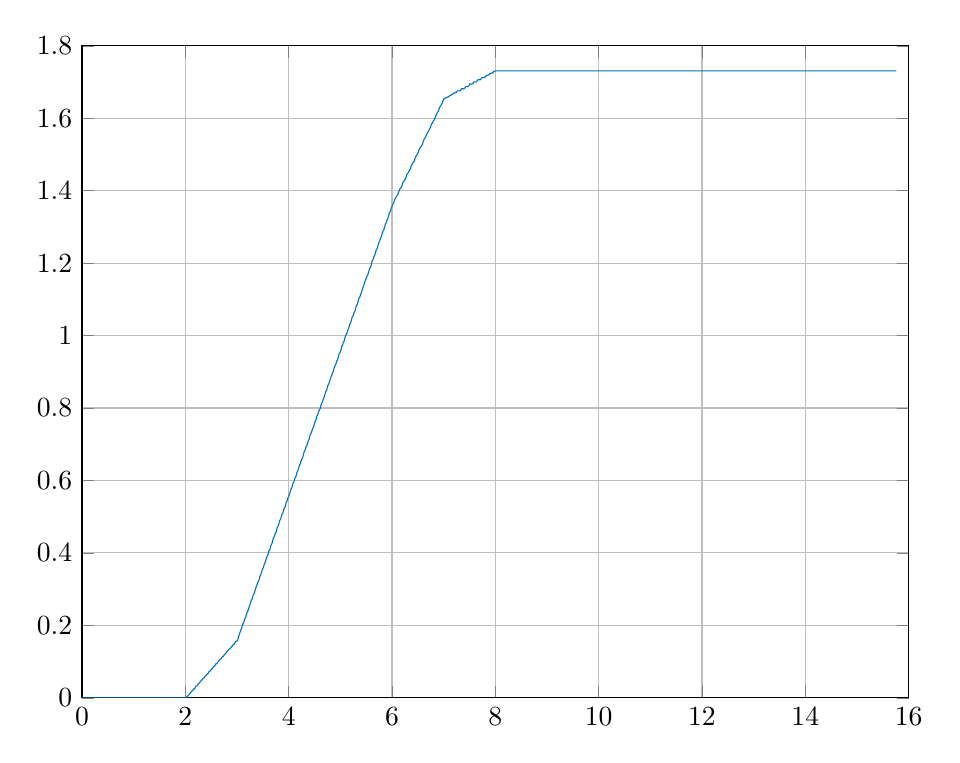
\begin{tikzpicture}

\begin{axis}[%
width=4.133in,
height=3.26in,
at={(0.693in,0.44in)},
scale only axis,
xmin=0,
xmax=16,
xmajorgrids,
ymin=0,
ymax=1.8,
ymajorgrids,
axis background/.style={fill=white}
]
\addplot [color=mycolor1,solid,forget plot]
  table[row sep=crcr]{%
0	0\\
0.0176569919999996	0\\
0.0329493709999993	0\\
0.0483888879999993	0\\
0.0640940889999997	0\\
0.0798458949989993	0\\
0.0958887509999992	0\\
0.111983863000999	0\\
0.127921078	0\\
0.143937094	0\\
0.159972982	0\\
0.175995181001999	0\\
0.191998524999999	0\\
0.207984587001	0\\
0.224022642	0\\
0.240222648999999	0\\
0.255975674001	0\\
0.272023266	0\\
0.28799259	0\\
0.303978898999999	0\\
0.319895037001	0\\
0.336037301999999	0\\
0.352051528	0\\
0.367968793	0\\
0.383873009001	0\\
0.399862312999999	0\\
0.416022466000999	0\\
0.432019031999999	0\\
0.448131865999999	0\\
0.464108878	0\\
0.480017946	0\\
0.495980695999999	0\\
0.512107225999999	0\\
0.528123782999999	0\\
0.544085962001	0\\
0.560119726999999	0\\
0.575859410999999	0\\
0.592148155	0\\
0.608002543	0\\
0.624022842999999	0\\
0.640116214001999	0\\
0.656129908999999	0\\
0.672144375999999	0\\
0.688173236	0\\
0.704075804000999	0\\
0.719948993999	0\\
0.735902495001	0\\
0.752065337001001	0\\
0.768125969	0\\
0.784121853000999	0\\
0.800171049	0\\
0.815850642	0\\
0.831850273999999	0\\
0.849983964001999	0\\
0.865510083	0\\
0.881092908999999	0\\
0.896435076	0\\
0.911997679	0\\
0.927939124000999	0\\
0.943900099999999	0\\
0.959962982	0\\
0.976019297999999	0\\
0.991988354999999	0\\
1.012854596001	0\\
1.024756646001	0\\
1.040019611	0\\
1.056009953001	0\\
1.071876429	0\\
1.087908785999	0\\
1.104012500999	0\\
1.119895645	0\\
1.138221575001	0\\
1.153239963	0\\
1.168241496	0\\
1.183957946	0\\
1.200037747	0\\
1.21612978	0\\
1.232136003	0\\
1.248014692	0\\
1.263995738	0\\
1.279987829	0\\
1.296001795	0\\
1.312014753	0\\
1.327903034	0\\
1.344139308001	0\\
1.360180451	0\\
1.376046951	0\\
1.392069979	0\\
1.408125993999	0\\
1.424002318001	0\\
1.44001917	0\\
1.45601478	0\\
1.471984831	0\\
1.487998065001	0\\
1.503985741	0\\
1.520101146	0\\
1.536048301001	0\\
1.552229580001	0\\
1.568081369	0\\
1.583848599	0\\
1.601812136001	0\\
1.616659084001	0\\
1.631999078001	0\\
1.64799345	0\\
1.663992071	0\\
1.680104149	0\\
1.695972259001	0\\
1.712104698001	0\\
1.728148175	0\\
1.744128901	0\\
1.760143809	0\\
1.776073809	0\\
1.792004756	0\\
1.807993174	0\\
1.823948729001	0\\
1.839894647	0\\
1.856088458	0\\
1.872161898	0\\
1.888054448	0\\
1.904106139	0\\
1.920131741	0\\
1.936119843	0\\
1.952172406	0\\
1.968225336	0\\
1.98413279	0\\
2.000128369	0\\
2.017452882	0\\
2.032446061	0.00390433294924698\\
2.047875513	0.00585517154729405\\
2.06600351	0.00780866589849396\\
2.080914502001	0.0106291984121417\\
2.095930835001	0.0125827275282714\\
2.111988129001	0.0164869086612016\\
2.127986805	0.0184377115318521\\
2.143954752	0.0203910115128039\\
2.160004057	0.0242950407104893\\
2.175998709001	0.0242949317077637\\
2.192023644999	0.0290702337901097\\
2.208107203	0.0329741109336267\\
2.224123459001	0.0329741923720712\\
2.24022796	0.036877981202997\\
2.256002237	0.038828511649299\\
2.271972199	0.0407817061734266\\
2.288150769	0.0446851185623389\\
2.304156243999	0.0470779880077378\\
2.319861292	0.0494616007905821\\
2.337960481	0.0533652359931435\\
2.352805525001	0.0533652359931435\\
2.367983794001	0.0572686562606604\\
2.383994642	0.0592190017233775\\
2.399981156	0.0611718323670802\\
2.418295247	0.0655181971000198\\
2.433350862	0.0659495310646595\\
2.448501446	0.069852769856491\\
2.464074613999	0.0737558849454751\\
2.480054312	0.0737558921134628\\
2.495913975	0.0776588222848839\\
2.511954783999	0.0796089662046497\\
2.527945517	0.0820054175958334\\
2.544035074	0.0863405767662179\\
2.560071536	0.0863405767662179\\
2.576054206	0.0902434300838667\\
2.592017366	0.0941460822889776\\
2.607987462	0.0941460822889776\\
2.624127293	0.0980487387184567\\
2.639906073	0.100443179453319\\
2.656088473001	0.102828650695435\\
2.672128708	0.106731154000643\\
2.688122867001	0.106731233593803\\
2.704055790999	0.110633606352522\\
2.720109552	0.114535956414582\\
2.736132303	0.11453588310037\\
2.752055242001	0.118883424832506\\
2.768000863	0.120833180740616\\
2.784012373	0.123219296616339\\
2.800107231999	0.127121388448612\\
2.816064094	0.129071066576203\\
2.831929742001	0.131023392570497\\
2.847829863	0.134925173246418\\
2.865948319	0.135371333215796\\
2.881293705	0.139273030103667\\
2.896822617001	0.141657209037872\\
2.912293753	0.143609422550279\\
2.928141126	0.147511158451068\\
2.944129975	0.147511068046037\\
2.960105376	0.151412650109362\\
2.976130227	0.155761072653752\\
2.992155335	0.155760912645771\\
3.014058361999	0.160097702630488\\
3.026151745	0.167864959020466\\
3.041511649	0.173698467056526\\
3.057165543	0.180502817397262\\
3.072486670001	0.186820619976893\\
3.088069915001	0.191169210427742\\
3.104130961	0.200888596486791\\
3.120140283001	0.20520629618721\\
3.136113861999	0.21104412872734\\
3.152134477999	0.218811623657632\\
3.168112055	0.222227833297958\\
3.184195113	0.23194720518924\\
3.200006735001	0.236277474394535\\
3.216001758	0.242115004404733\\
3.232046784	0.25031962232378\\
3.248055262	0.256153544052136\\
3.264002116	0.263453708730698\\
3.280096163	0.271221357052618\\
3.295973764	0.273172793273993\\
3.312002098	0.283341684735301\\
3.327947942	0.287224128199225\\
3.343859488	0.293499047980144\\
3.360094537001	0.301765348438743\\
3.375961174	0.308561718082721\\
3.391939837	0.314398969754547\\
3.408027968	0.320230150900805\\
3.423981933	0.32456855917289\\
3.439959516001	0.334288525205991\\
3.456013447	0.338171313688702\\
3.472003897	0.345430410886236\\
3.488076603001	0.353673889437244\\
3.504151179	0.357567900238369\\
3.520151864	0.365345082321775\\
3.536141274	0.371627300996949\\
3.552010337	0.375515904192678\\
3.568003997	0.386218312655512\\
3.583913766	0.391014534830087\\
3.601898940001	0.396851491115481\\
3.617405785	0.406571757693649\\
3.632910511001	0.408512094977957\\
3.648194348	0.416743398089045\\
3.664158906	0.423071266519109\\
3.680183246	0.427444534159687\\
3.695966354	0.438078223466569\\
3.711966813	0.44196172340052\\
3.727970744	0.447798517776825\\
3.743994990001	0.455568256527589\\
3.759982887	0.457971189292492\\
3.776008374	0.468671210038401\\
3.791994251	0.473027495506769\\
3.808099147	0.4793049220955\\
3.824023096001	0.48902549783394\\
3.840693448	0.492909644481979\\
3.856181481	0.498746125165715\\
3.872149407	0.507476747481962\\
3.888242151	0.509897647425451\\
3.903977811001	0.520090487230618\\
3.920287342	0.524416153188937\\
3.936407333	0.530252693442584\\
3.952240439	0.539973494240862\\
3.968113205	0.54286472806316\\
3.984072015	0.55112469215621\\
4.000137102	0.55695701787624\\
4.017858345	0.563260643466085\\
4.033294948	0.571480107657188\\
4.049006477999	0.577312781034043\\
4.064496412001	0.581694759571203\\
4.080532356	0.591869857805512\\
4.095879986	0.594295273360013\\
4.112166320001	0.602543611728273\\
4.127908479	0.608376457890891\\
4.143892742	0.612707994787116\\
4.159886279	0.622429803515008\\
4.175867102	0.626807909240167\\
4.191988215	0.633578235570502\\
4.207981271	0.641361836148435\\
4.22390618	0.645714101854798\\
4.239896447	0.653492265547584\\
4.255914538	0.659769398587324\\
4.271894383	0.664150201824488\\
4.287957467	0.673872642778242\\
4.303943203999	0.68063882142053\\
4.319862047001	0.684527476912805\\
4.337956433001	0.694719252567991\\
4.353400467	0.696663252889453\\
4.368940805	0.704886283122997\\
4.384287624	0.711211998944977\\
4.400130668	0.715580306883645\\
4.41611688	0.725754643473425\\
4.432395656	0.730108852984099\\
4.448132880001	0.735945901749324\\
4.464115124001	0.743730337351738\\
4.480260387001	0.74660498133247\\
4.496012007999	0.756328387994689\\
4.512048174	0.76264233457461\\
4.52799622	0.766981595904035\\
4.544016265	0.777172677751638\\
4.560127797	0.781059105999237\\
4.575869669001	0.787386478138426\\
4.594142836	0.795617005419401\\
4.609555252001	0.798034540019222\\
4.625139464	0.807758804499379\\
4.640547507	0.814043789808897\\
4.656131845	0.818399315978372\\
4.672259648	0.826184415332106\\
4.688269344001	0.830557586611065\\
4.704133365	0.838783701244969\\
4.720172814	0.847046710809381\\
4.736259514001	0.848986017725552\\
4.752166237	0.859625801359261\\
4.768111973	0.865461864754158\\
4.7840954	0.869838998730332\\
4.800111164	0.877624115285728\\
4.816085519999	0.884375444388268\\
4.832931725	0.890213186306615\\
4.848126440001	0.897998810716499\\
4.864355088	0.900852118824062\\
4.88013147	0.911065271980985\\
4.895956453	0.916901633888892\\
4.911998776	0.920790171741931\\
4.928141044001	0.929500747882171\\
4.944161534	0.93338535065637\\
4.959976506	0.941165878418975\\
4.976036742	0.949864341168747\\
4.991939937	0.952290933972765\\
5.016354084	0.962016549107349\\
5.025515898	0.97027851173527\\
5.040948717	0.972667026005746\\
5.056337351	0.980453537713622\\
5.072586752	0.984803016453124\\
5.088045262	0.993517245493705\\
5.104213663	1.00130390356731\\
5.120011865	1.00324390244501\\
5.136027073001	1.01150548768494\\
5.151995621	1.01778878477608\\
5.168132084001	1.02362092863932\\
5.184104115001	1.03187150367144\\
5.200173125001	1.0347431206067\\
5.216127875999	1.04447082094826\\
5.23214981	1.05225828475031\\
5.247998842	1.05467267804059\\
5.263963627	1.06290771004356\\
5.279941836	1.06679367844988\\
5.296030691999	1.07552364212592\\
5.312337375	1.08375695170035\\
5.327888942	1.08569728954688\\
5.345917909	1.0958991283246\\
5.361274315001	1.10368761774985\\
5.376693919001	1.10607454042285\\
5.392199278	1.11386304460273\\
5.408445905	1.11869547509512\\
5.424153086	1.12692329317076\\
5.440124315	1.13471182261864\\
5.456135309001	1.13907114342865\\
5.472194858001	1.14685482543498\\
5.488131944	1.15508961449501\\
5.504169974	1.15797491827531\\
5.520185529	1.16576436312931\\
5.536119488	1.17009464855185\\
5.552140144	1.17835060009905\\
5.567948917	1.18614036295476\\
5.583855777	1.18808098457155\\
5.600125222	1.19631571174139\\
5.616102575	1.20698990369254\\
5.632119532001	1.20893074821909\\
5.647968349	1.21716336068644\\
5.663988158	1.22152194919517\\
5.680163063	1.22930691836315\\
5.696138497	1.23709723104423\\
5.712146018	1.23996445916086\\
5.728155473001	1.24821493436175\\
5.744013836	1.2560026602579\\
5.759982835	1.26032944285187\\
5.776099253	1.26859109883883\\
5.792016785	1.27247808804642\\
5.807984184999	1.28026410053088\\
5.824005104001	1.28898035976636\\
5.839901941999	1.29138016604068\\
5.856111191	1.29917140478369\\
5.872137605	1.30787167155932\\
5.888109895	1.31175665269766\\
5.904078052999	1.31954812213739\\
5.920136468	1.3239170246541\\
5.936139194	1.33214621044253\\
5.952150468	1.34039599330195\\
5.968112747	1.34233742626511\\
5.984118093	1.35103970484357\\
6.000169393001	1.35687809372251\\
6.017907359	1.36319440514874\\
6.033298158	1.36708557340685\\
6.048817914	1.37338172195563\\
6.064313506	1.37921828815248\\
6.079858372	1.38310961808194\\
6.095938104	1.38551915707463\\
6.112129856001	1.38985260280745\\
6.128122594001	1.39617133507081\\
6.144148312	1.40200800683068\\
6.160126	1.40635606084335\\
6.176118692	1.40829782875498\\
6.191997856999	1.41265739059861\\
6.207988456	1.4223915642376\\
6.223954487	1.42433341573849\\
6.239980696	1.42870399165313\\
6.256161189	1.43259243300577\\
6.272186881	1.43737542181974\\
6.288102795	1.44516884318294\\
6.304106877999	1.44757706719264\\
6.320091327001	1.45146920370073\\
6.335880024	1.45583670268911\\
6.354022728001	1.45972264555965\\
6.369367339	1.46751638896153\\
6.384656037001	1.47186130930087\\
6.400487399	1.47574772445172\\
6.416146967	1.48010621122126\\
6.432134884	1.48204839648761\\
6.448258582	1.49031916400666\\
6.464230844	1.49465069594643\\
6.480140403	1.49853794854387\\
6.496101925	1.50288465186036\\
6.512133170001	1.50723996163288\\
6.527995276001	1.5150288246788\\
6.544131765	1.5193983322338\\
6.560232872	1.52133968307788\\
6.575928129001	1.52523262320056\\
6.591886065001	1.52912285175324\\
6.607860364	1.53780535525859\\
6.624081188	1.54216330969375\\
6.64010489	1.54605370056762\\
6.656124651	1.55041680942208\\
6.672092688	1.55626018920918\\
6.688149902	1.56015370583862\\
6.704156666	1.56449954484565\\
6.720119616	1.56838992268183\\
6.736130569999	1.5727421715732\\
6.752110960001	1.57906073275119\\
6.768194147	1.58490200586405\\
6.784095092	1.58684747669556\\
6.800197348	1.59312543997057\\
6.816194575	1.59506792706893\\
6.831859841	1.60136448089541\\
6.849828911	1.60766993116336\\
6.864617671	1.61203172473624\\
6.880157518	1.61592562528306\\
6.896009697	1.61981682598521\\
6.911887272	1.62566297660441\\
6.928104079	1.63195165487883\\
6.944126318	1.6343574870702\\
6.960239648	1.63916444535016\\
6.975996271	1.64305596915393\\
6.992085988	1.6508463075032\\
7.016386174001	1.65473990859966\\
7.025061271	1.65473990859966\\
7.040185025001	1.65668300683965\\
7.056043985	1.65668300683965\\
7.071893242	1.65863151113391\\
7.087855755	1.65863151113391\\
7.105810378	1.6605773859973\\
7.121061536	1.66297140664221\\
7.136383799001	1.66297140664221\\
7.152026429001	1.66491991093647\\
7.167978459	1.66538204837926\\
7.184012490001	1.66780159953478\\
7.199993055	1.66974469777478\\
7.215994312	1.66974469777478\\
7.23196481	1.67169320206904\\
7.247999733001	1.67169320206904\\
7.264007369	1.67558217517242\\
7.279991372	1.67558217517242\\
7.296000797	1.67558217517242\\
7.311999573	1.67558217517242\\
7.327922423	1.67753067946668\\
7.343911334001	1.68141965257006\\
7.359973346001	1.68141965257006\\
7.375992389001	1.68141965257006\\
7.391985549	1.68141965257006\\
7.407900927	1.68336815686432\\
7.423973568	1.68725712996771\\
7.439948952001	1.68725712996771\\
7.456101485	1.68725712996771\\
7.472080807	1.68770805237262\\
7.48796155	1.68965655666688\\
7.504134006	1.69448134350519\\
7.520200922001	1.69448134350519\\
7.536098779	1.69448134350519\\
7.552104697	1.69448134350519\\
7.56827453	1.69642984779945\\
7.583853204	1.70031882090283\\
7.601824367	1.70031882090283\\
7.616695095	1.70031882090283\\
7.631807787001	1.70031882090283\\
7.650056005	1.70421042343709\\
7.665368056002	1.70615629830048\\
7.68076289	1.70615629830048\\
7.696230869	1.70615629830048\\
7.712131819	1.70615629830048\\
7.728123589	1.71004790083473\\
7.743872118	1.71199377569812\\
7.762071043	1.71199377569812\\
7.777349242001	1.71199377569812\\
7.792729312	1.71199377569812\\
7.808310252	1.71635905452451\\
7.823859635	1.71680997692942\\
7.841935676	1.7192179892356\\
7.857040253	1.7192179892356\\
7.872569601	1.7192179892356\\
7.888079409	1.72310959176986\\
7.904135455	1.72310959176986\\
7.920105585999	1.72505546663324\\
7.936019375	1.72505546663324\\
7.951998727	1.72505546663324\\
7.968023823	1.7289470691675\\
7.984130769	1.7289470691675\\
8.00014034	1.73089294403089\\
8.017821677999	1.73089294403089\\
8.033098724	1.73089294403089\\
8.048316963	1.73089294403089\\
8.064003196	1.73089294403089\\
8.079857304001	1.73089294403089\\
8.098020238	1.73089294403089\\
8.113108572	1.73089294403089\\
8.128619412001	1.73089294403089\\
8.144172464002	1.73089294403089\\
8.160098947	1.73089294403089\\
8.176138305	1.73089294403089\\
8.192159091	1.73089294403089\\
8.208242679001	1.73089294403089\\
8.224136954	1.73089294403089\\
8.240136417001	1.73089294403089\\
8.256138591	1.73089294403089\\
8.272012499001	1.73089294403089\\
8.287949746	1.73089294403089\\
8.303986488001	1.73089294403089\\
8.320059948	1.73089294403089\\
8.335924213	1.73089294403089\\
8.352082102	1.73089294403089\\
8.368123696	1.73089294403089\\
8.384134268001	1.73089294403089\\
8.400099674	1.73089294403089\\
8.416171035	1.73089294403089\\
8.43210339	1.73089294403089\\
8.448250623	1.73089294403089\\
8.464174158	1.73089294403089\\
8.480013418	1.73089294403089\\
8.49606959	1.73089294403089\\
8.51209467	1.73089294403089\\
8.528188883	1.73089294403089\\
8.54414379	1.73089294403089\\
8.560263644999	1.73089294403089\\
8.575944886001	1.73089294403089\\
8.591893836	1.73089294403089\\
8.608100531	1.73089294403089\\
8.624120981	1.73089294403089\\
8.640017191999	1.73089294403089\\
8.655986086	1.73089294403089\\
8.672105941001	1.73089294403089\\
8.688114039	1.73089294403089\\
8.704057369	1.73089294403089\\
8.720092849001	1.73089294403089\\
8.73607862	1.73089294403089\\
8.751981875	1.73089294403089\\
8.767940771001	1.73089294403089\\
8.784107483	1.73089294403089\\
8.800101844001	1.73089294403089\\
8.815980264001	1.73089294403089\\
8.831927292	1.73089294403089\\
8.848216319999	1.73089294403089\\
8.864169067	1.73089294403089\\
8.880143524	1.73089294403089\\
8.896233537001	1.73089294403089\\
8.91194638	1.73089294403089\\
8.928108737	1.73089294403089\\
8.944113401	1.73089294403089\\
8.960101669	1.73089294403089\\
8.976327881	1.73089294403089\\
8.99209848	1.73089294403089\\
9.013952268001	1.73089294403089\\
9.025773552	1.73089294403089\\
9.040869478001	1.73089294403089\\
9.056036434999	1.73089294403089\\
9.071914411	1.73089294403089\\
9.087853324	1.73089294403089\\
9.105810976	1.73089294403089\\
9.120858639	1.73089294403089\\
9.13632967	1.73089294403089\\
9.15201243	1.73089294403089\\
9.167999229	1.73089294403089\\
9.183965557	1.73089294403089\\
9.200132063	1.73089294403089\\
9.215995793	1.73089294403089\\
9.231992385	1.73089294403089\\
9.247949988001	1.73089294403089\\
9.263959078	1.73089294403089\\
9.280023528001	1.73089294403089\\
9.296031565001	1.73089294403089\\
9.312019722	1.73089294403089\\
9.330415196	1.73089294403089\\
9.345603137	1.73089294403089\\
9.360958531	1.73089294403089\\
9.376435224	1.73089294403089\\
9.392127622	1.73089294403089\\
9.40803013	1.73089294403089\\
9.423964234	1.73089294403089\\
9.440126291	1.73089294403089\\
9.456176990001	1.73089294403089\\
9.472130308	1.73089294403089\\
9.488090294	1.73089294403089\\
9.504025634	1.73089294403089\\
9.520107689	1.73089294403089\\
9.536156759	1.73089294403089\\
9.552134793	1.73089294403089\\
9.568032706	1.73089294403089\\
9.583886257999	1.73089294403089\\
9.601893501	1.73089294403089\\
9.616751991	1.73089294403089\\
9.631802068001	1.73089294403089\\
9.649949327	1.73089294403089\\
9.665047955	1.73089294403089\\
9.68017228	1.73089294403089\\
9.696123554001	1.73089294403089\\
9.712203729	1.73089294403089\\
9.728291733	1.73089294403089\\
9.744064056	1.73089294403089\\
9.76029346	1.73089294403089\\
9.776216049001	1.73089294403089\\
9.792114487	1.73089294403089\\
9.808005019	1.73089294403089\\
9.824057947	1.73089294403089\\
9.839899741	1.73089294403089\\
9.856131367001	1.73089294403089\\
9.87208259	1.73089294403089\\
9.888036154	1.73089294403089\\
9.903991547001	1.73089294403089\\
9.920274755	1.73089294403089\\
9.935971294	1.73089294403089\\
9.952104440001	1.73089294403089\\
9.968090718	1.73089294403089\\
9.984153404	1.73089294403089\\
10.000027398	1.73089294403089\\
10.017745163	1.73089294403089\\
10.033166296	1.73089294403089\\
10.049156983001	1.73089294403089\\
10.064389868999	1.73089294403089\\
10.079857773002	1.73089294403089\\
10.098077035	1.73089294403089\\
10.113209864	1.73089294403089\\
10.128525625	1.73089294403089\\
10.143979194999	1.73089294403089\\
10.159933856	1.73089294403089\\
10.17593601	1.73089294403089\\
10.192002685	1.73089294403089\\
10.207984563	1.73089294403089\\
10.223974093	1.73089294403089\\
10.239999014001	1.73089294403089\\
10.255954391001	1.73089294403089\\
10.271959051	1.73089294403089\\
10.2879723	1.73089294403089\\
10.303942492001	1.73089294403089\\
10.32003706	1.73089294403089\\
10.335888222	1.73089294403089\\
10.351879085	1.73089294403089\\
10.370070283001	1.73089294403089\\
10.38563901	1.73089294403089\\
10.401102127	1.73089294403089\\
10.416405423	1.73089294403089\\
10.431975333	1.73089294403089\\
10.448221289	1.73089294403089\\
10.464387014	1.73089294403089\\
10.480258782	1.73089294403089\\
10.496044526	1.73089294403089\\
10.512210391	1.73089294403089\\
10.528057609	1.73089294403089\\
10.544017672	1.73089294403089\\
10.560037907001	1.73089294403089\\
10.575849163	1.73089294403089\\
10.591870081	1.73089294403089\\
10.607902650001	1.73089294403089\\
10.623901751	1.73089294403089\\
10.640037912001	1.73089294403089\\
10.656072916	1.73089294403089\\
10.671987441	1.73089294403089\\
10.687948452	1.73089294403089\\
10.703983599999	1.73089294403089\\
10.719994529	1.73089294403089\\
10.738421561001	1.73089294403089\\
10.753977815	1.73089294403089\\
10.769343131	1.73089294403089\\
10.785264051001	1.73089294403089\\
10.800593802	1.73089294403089\\
10.816036749001	1.73089294403089\\
10.831931327	1.73089294403089\\
10.847834997	1.73089294403089\\
10.864280258	1.73089294403089\\
10.88015102	1.73089294403089\\
10.896045820001	1.73089294403089\\
10.91226938	1.73089294403089\\
10.928436823001	1.73089294403089\\
10.944201509	1.73089294403089\\
10.95996539	1.73089294403089\\
10.976080183001	1.73089294403089\\
10.991834655	1.73089294403089\\
11.012838194	1.73089294403089\\
11.024809476001	1.73089294403089\\
11.039959547	1.73089294403089\\
11.055957389	1.73089294403089\\
11.071948585	1.73089294403089\\
11.087850294	1.73089294403089\\
11.105849678	1.73089294403089\\
11.121228682	1.73089294403089\\
11.136497820001	1.73089294403089\\
11.152016327	1.73089294403089\\
11.168001477	1.73089294403089\\
11.184048563	1.73089294403089\\
11.200010456	1.73089294403089\\
11.215941071	1.73089294403089\\
11.232021739	1.73089294403089\\
11.247996732	1.73089294403089\\
11.264008092	1.73089294403089\\
11.280011784	1.73089294403089\\
11.296020358	1.73089294403089\\
11.312011326	1.73089294403089\\
11.327870831	1.73089294403089\\
11.344017193	1.73089294403089\\
11.360094827	1.73089294403089\\
11.37602354	1.73089294403089\\
11.392001935	1.73089294403089\\
11.410273615	1.73089294403089\\
11.425311660001	1.73089294403089\\
11.440344288001	1.73089294403089\\
11.456066322	1.73089294403089\\
11.471984105	1.73089294403089\\
11.488095711	1.73089294403089\\
11.504067401	1.73089294403089\\
11.519993433	1.73089294403089\\
11.536047279	1.73089294403089\\
11.552133859	1.73089294403089\\
11.568066832001	1.73089294403089\\
11.583962507001	1.73089294403089\\
11.600136584001	1.73089294403089\\
11.616145073	1.73089294403089\\
11.632107806002	1.73089294403089\\
11.648126076	1.73089294403089\\
11.664158297	1.73089294403089\\
11.680125306002	1.73089294403089\\
11.69610744	1.73089294403089\\
11.712090506	1.73089294403089\\
11.728128431002	1.73089294403089\\
11.744128114	1.73089294403089\\
11.760006242	1.73089294403089\\
11.776142265	1.73089294403089\\
11.792119397	1.73089294403089\\
11.808000456	1.73089294403089\\
11.824031265	1.73089294403089\\
11.839848429001	1.73089294403089\\
11.856126639	1.73089294403089\\
11.872139873	1.73089294403089\\
11.888061124001	1.73089294403089\\
11.903977892	1.73089294403089\\
11.919977171	1.73089294403089\\
11.936120651001	1.73089294403089\\
11.95212071	1.73089294403089\\
11.968112159	1.73089294403089\\
11.984110299	1.73089294403089\\
12.000148144	1.73089294403089\\
12.017616178	1.73089294403089\\
12.032916413	1.73089294403089\\
12.048062868	1.73089294403089\\
12.064247145	1.73089294403089\\
12.080031565	1.73089294403089\\
12.095857071	1.73089294403089\\
12.114326913	1.73089294403089\\
12.129717386001	1.73089294403089\\
12.145185605	1.73089294403089\\
12.160579526001	1.73089294403089\\
12.17615743	1.73089294403089\\
12.192044001	1.73089294403089\\
12.208107384001	1.73089294403089\\
12.22413264	1.73089294403089\\
12.239998831	1.73089294403089\\
12.255977817	1.73089294403089\\
12.2721318	1.73089294403089\\
12.288124999	1.73089294403089\\
12.304199958	1.73089294403089\\
12.320089918	1.73089294403089\\
12.335957526	1.73089294403089\\
12.351868006	1.73089294403089\\
12.369889144	1.73089294403089\\
12.384847655	1.73089294403089\\
12.400397941	1.73089294403089\\
12.416186185	1.73089294403089\\
12.431919914	1.73089294403089\\
12.44785488	1.73089294403089\\
12.463938831	1.73089294403089\\
12.479899877001	1.73089294403089\\
12.495942601001	1.73089294403089\\
12.512133109	1.73089294403089\\
12.528007368	1.73089294403089\\
12.544011131	1.73089294403089\\
12.560281362	1.73089294403089\\
12.575907096001	1.73089294403089\\
12.591862366	1.73089294403089\\
12.60982631	1.73089294403089\\
12.624998969	1.73089294403089\\
12.640364281	1.73089294403089\\
12.656007152	1.73089294403089\\
12.671985826	1.73089294403089\\
12.687989543	1.73089294403089\\
12.703979845	1.73089294403089\\
12.719979999	1.73089294403089\\
12.735987726	1.73089294403089\\
12.752109847	1.73089294403089\\
12.76800151	1.73089294403089\\
12.784026486	1.73089294403089\\
12.800316457001	1.73089294403089\\
12.816193657	1.73089294403089\\
12.831856733	1.73089294403089\\
12.847815061999	1.73089294403089\\
12.86586973	1.73089294403089\\
12.881389498	1.73089294403089\\
12.896081717999	1.73089294403089\\
12.912021732	1.73089294403089\\
12.928021265	1.73089294403089\\
12.943976738	1.73089294403089\\
12.959968183	1.73089294403089\\
12.975981392	1.73089294403089\\
12.991952190001	1.73089294403089\\
13.014032231	1.73089294403089\\
13.025912447	1.73089294403089\\
13.040991474	1.73089294403089\\
13.05616441	1.73089294403089\\
13.072004754001	1.73089294403089\\
13.088577986	1.73089294403089\\
13.104128119	1.73089294403089\\
13.120102924001	1.73089294403089\\
13.136021110001	1.73089294403089\\
13.151991805	1.73089294403089\\
13.167992495	1.73089294403089\\
13.183989793	1.73089294403089\\
13.200120648002	1.73089294403089\\
13.21613913	1.73089294403089\\
13.232192535	1.73089294403089\\
13.248139052	1.73089294403089\\
13.264262571	1.73089294403089\\
13.280250914	1.73089294403089\\
13.296000811	1.73089294403089\\
13.312133867001	1.73089294403089\\
13.330739937	1.73089294403089\\
13.345647581	1.73089294403089\\
13.360595819999	1.73089294403089\\
13.376198595	1.73089294403089\\
13.39222434	1.73089294403089\\
13.408155114	1.73089294403089\\
13.424150148002	1.73089294403089\\
13.440136007	1.73089294403089\\
13.456188839002	1.73089294403089\\
13.472003998	1.73089294403089\\
13.488095885	1.73089294403089\\
13.504196046	1.73089294403089\\
13.520096960999	1.73089294403089\\
13.536167785	1.73089294403089\\
13.552102566	1.73089294403089\\
13.568163644	1.73089294403089\\
13.584796876	1.73089294403089\\
13.599831254001	1.73089294403089\\
13.618245261001	1.73089294403089\\
13.633722624001	1.73089294403089\\
13.649157611001	1.73089294403089\\
13.664655997	1.73089294403089\\
13.680177298	1.73089294403089\\
13.696123715	1.73089294403089\\
13.712307977	1.73089294403089\\
13.727970328	1.73089294403089\\
13.743982544	1.73089294403089\\
13.759982552	1.73089294403089\\
13.776111122	1.73089294403089\\
13.792130539	1.73089294403089\\
13.807974729	1.73089294403089\\
13.82405422	1.73089294403089\\
13.841393413	1.73089294403089\\
13.856378463	1.73089294403089\\
13.872157671	1.73089294403089\\
13.887957688	1.73089294403089\\
13.904130582001	1.73089294403089\\
13.920127753	1.73089294403089\\
13.936001875	1.73089294403089\\
13.952010167	1.73089294403089\\
13.968102957001	1.73089294403089\\
13.984115354	1.73089294403089\\
14.000155619	1.73089294403089\\
14.016141312	1.73089294403089\\
14.032078482	1.73089294403089\\
14.048136593	1.73089294403089\\
14.064139058	1.73089294403089\\
14.08001677	1.73089294403089\\
14.095890900001	1.73089294403089\\
14.112129435	1.73089294403089\\
14.128130840001	1.73089294403089\\
14.144111039	1.73089294403089\\
14.160233269999	1.73089294403089\\
14.176252287001	1.73089294403089\\
14.192047943001	1.73089294403089\\
14.208015684001	1.73089294403089\\
14.224007239	1.73089294403089\\
14.23998584	1.73089294403089\\
14.256104202	1.73089294403089\\
14.272076002001	1.73089294403089\\
14.288047094	1.73089294403089\\
14.304102915999	1.73089294403089\\
14.320136792001	1.73089294403089\\
14.337714891	1.73089294403089\\
14.353145339	1.73089294403089\\
14.368848356	1.73089294403089\\
14.384096497	1.73089294403089\\
14.400035673	1.73089294403089\\
14.415997125	1.73089294403089\\
14.431997244	1.73089294403089\\
14.448077771	1.73089294403089\\
14.464095926	1.73089294403089\\
14.48025505	1.73089294403089\\
14.496042989	1.73089294403089\\
14.512007292	1.73089294403089\\
14.527996205999	1.73089294403089\\
14.544107733	1.73089294403089\\
14.560114362	1.73089294403089\\
14.576034194	1.73089294403089\\
14.592043113	1.73089294403089\\
14.608107147	1.73089294403089\\
14.62414413	1.73089294403089\\
14.640012526	1.73089294403089\\
14.656124368	1.73089294403089\\
14.672068295	1.73089294403089\\
14.688113908	1.73089294403089\\
14.704103528	1.73089294403089\\
14.720132618001	1.73089294403089\\
14.736101291	1.73089294403089\\
14.752014233	1.73089294403089\\
14.767998481001	1.73089294403089\\
14.78400056	1.73089294403089\\
14.799989955	1.73089294403089\\
14.816103842	1.73089294403089\\
14.831900654	1.73089294403089\\
14.847882925	1.73089294403089\\
14.864075212	1.73089294403089\\
14.880124575001	1.73089294403089\\
14.89600567	1.73089294403089\\
14.912006696	1.73089294403089\\
14.928128286	1.73089294403089\\
14.944095445001	1.73089294403089\\
14.960153150001	1.73089294403089\\
14.976165447	1.73089294403089\\
14.992167395	1.73089294403089\\
15.016628752	1.73089294403089\\
15.025324941	1.73089294403089\\
15.040619912001	1.73089294403089\\
15.056011774	1.73089294403089\\
15.072047940001	1.73089294403089\\
15.088400132	1.73089294403089\\
15.103882531	1.73089294403089\\
15.120005512	1.73089294403089\\
15.136037931002	1.73089294403089\\
15.152021778	1.73089294403089\\
15.167985006	1.73089294403089\\
15.184058858	1.73089294403089\\
15.200017583	1.73089294403089\\
15.215996043	1.73089294403089\\
15.232018428	1.73089294403089\\
15.247967779	1.73089294403089\\
15.264006795	1.73089294403089\\
15.280026709	1.73089294403089\\
15.29603172	1.73089294403089\\
15.311989483	1.73089294403089\\
15.328026196	1.73089294403089\\
15.344016146	1.73089294403089\\
15.360000124001	1.73089294403089\\
15.37598327	1.73089294403089\\
15.392019391	1.73089294403089\\
15.408003634001	1.73089294403089\\
15.423980631	1.73089294403089\\
15.439884946	1.73089294403089\\
15.455929379001	1.73089294403089\\
15.471968413	1.73089294403089\\
15.487887537001	1.73089294403089\\
15.506121751	1.73089294403089\\
15.521468338	1.73089294403089\\
15.536813265	1.73089294403089\\
15.552169837	1.73089294403089\\
15.56818953	1.73089294403089\\
15.584386016001	1.73089294403089\\
15.600109606999	1.73089294403089\\
15.616152769	1.73089294403089\\
15.632049249	1.73089294403089\\
15.647982221001	1.73089294403089\\
15.664276627	1.73089294403089\\
15.680109623	1.73089294403089\\
15.696136287001	1.73089294403089\\
15.712413599	1.73089294403089\\
15.728203662001	1.73089294403089\\
15.74423624	1.73089294403089\\
15.760140623	1.73089294403089\\
};
\end{axis}
\end{tikzpicture}%}
      \caption{The error in displacement of the robot over time for
        $(K_{\Psi}^R, K_{\omega}^T) \equiv (0.5 K_{\Psi, max}^R, 0.5 K_{\omega, max}^T)$}
      \label{fig:19_11_distance}
    \end{figure}
  \end{minipage}
  \hfill
  \begin{minipage}{0.45\linewidth}
    \begin{figure}[H]
      \scalebox{0.6}{% This file was created by matlab2tikz.
%
%The latest updates can be retrieved from
%  http://www.mathworks.com/matlabcentral/fileexchange/22022-matlab2tikz-matlab2tikz
%where you can also make suggestions and rate matlab2tikz.
%
\definecolor{mycolor1}{rgb}{0.00000,0.44700,0.74100}%
%
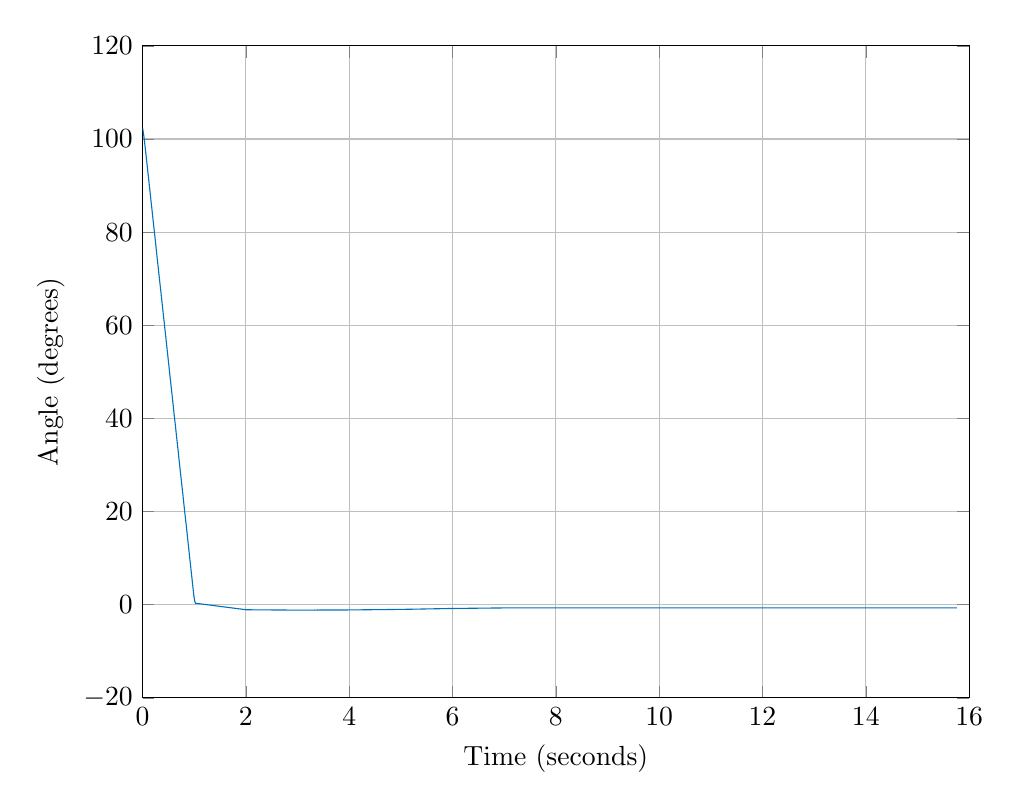
\begin{tikzpicture}

\begin{axis}[%
width=4.133in,
height=3.26in,
at={(0.693in,0.44in)},
scale only axis,
xmin=0,
xmax=16,
xmajorgrids,
xlabel={Time (seconds)},
ymin=-20,
ymax=120,
ymajorgrids,
ylabel={Angle (degrees)},
axis background/.style={fill=white}
]
\addplot [color=mycolor1,solid,forget plot]
  table[row sep=crcr]{%
0	102.4204\\
0.0176569919999996	101.1844\\
0.0329493709999993	99.9444\\
0.0483888879999993	98.4384\\
0.0640940889999997	96.8684\\
0.0798458949989993	95.2704\\
0.0958887509999992	93.6444\\
0.111983863000999	92.0144\\
0.127921078	90.3744\\
0.143937094	88.7464\\
0.159972982	87.0964\\
0.175995181001999	85.4644\\
0.191998524999999	83.8384\\
0.207984587001	82.2004\\
0.224022642	80.5584\\
0.240222648999999	78.9264\\
0.255975674001	77.2884\\
0.272023266	75.5804\\
0.28799259	73.9104\\
0.303978898999999	72.3004\\
0.319895037001	70.6944\\
0.336037301999999	69.0824\\
0.352051528	67.4584\\
0.367968793	65.8184\\
0.383873009001	64.1764\\
0.399862312999999	62.5564\\
0.416022466000999	60.9144\\
0.432019031999999	59.2664\\
0.448131865999999	57.6544\\
0.464108878	56.0044\\
0.480017946	54.3764\\
0.495980695999999	52.7244\\
0.512107225999999	51.0744\\
0.528123782999999	49.4004\\
0.544085962001	47.7884\\
0.560119726999999	46.1604\\
0.575859410999999	44.5424\\
0.592148155	42.9364\\
0.608002543	41.2284\\
0.624022842999999	39.6204\\
0.640116214001999	37.9864\\
0.656129908999999	36.3564\\
0.672144375999999	34.7224\\
0.688173236	33.1104\\
0.704075804000999	31.3864\\
0.719948993999	29.7844\\
0.735902495001	28.1684\\
0.752065337001001	26.5484\\
0.768125969	24.9204\\
0.784121853000999	23.2864\\
0.800171049	21.5844\\
0.815850642	19.9664\\
0.831850273999999	18.3524\\
0.849983964001999	16.6784\\
0.865510083	14.9944\\
0.881092908999999	13.3784\\
0.896435076	11.7684\\
0.911997679	10.1604\\
0.927939124000999	8.55840000000001\\
0.943900099999999	6.93039999999999\\
0.959962982	5.29039999999999\\
0.976019297999999	3.66239999999999\\
0.991988354999999	2.04040000000001\\
1.012854596001	0.6524\\
1.024756646001	0.306399999999982\\
1.040019611	0.288399999999982\\
1.056009953001	0.264399999999995\\
1.071876429	0.240399999999994\\
1.087908785999	0.220399999999998\\
1.104012500999	0.198399999999992\\
1.119895645	0.174399999999991\\
1.138221575001	0.148399999999995\\
1.153239963	0.12639999999999\\
1.168241496	0.106400000000008\\
1.183957946	0.084399999999988\\
1.200037747	0.0603999999999871\\
1.21612978	0.0364000000000004\\
1.232136003	0.0123999999999995\\
1.248014692	-0.0075999999999965\\
1.263995738	-0.0296000000000021\\
1.279987829	-0.053600000000003\\
1.296001795	-0.0776000000000039\\
1.312014753	-0.101600000000005\\
1.327903034	-0.121600000000015\\
1.344139308001	-0.145600000000016\\
1.360180451	-0.167600000000022\\
1.376046951	-0.191599999999994\\
1.392069979	-0.215600000000023\\
1.408125993999	-0.235600000000019\\
1.424002318001	-0.259600000000006\\
1.44001917	-0.281599999999997\\
1.45601478	-0.305599999999998\\
1.471984831	-0.329599999999999\\
1.487998065001	-0.351600000000005\\
1.503985741	-0.37360000000001\\
1.520101146	-0.395600000000016\\
1.536048301001	-0.419600000000017\\
1.552229580001	-0.443600000000018\\
1.568081369	-0.467600000000019\\
1.583848599	-0.4876\\
1.601812136001	-0.511600000000001\\
1.616659084001	-0.535600000000017\\
1.631999078001	-0.557600000000008\\
1.64799345	-0.581600000000009\\
1.663992071	-0.6036\\
1.680104149	-0.62360000000001\\
1.695972259001	-0.649600000000007\\
1.712104698001	-0.671600000000012\\
1.728148175	-0.695600000000013\\
1.744128901	-0.71759999999999\\
1.760143809	-0.74160000000002\\
1.776073809	-0.761600000000016\\
1.792004756	-0.785600000000002\\
1.807993174	-0.809600000000003\\
1.823948729001	-0.829599999999999\\
1.839894647	-0.851600000000005\\
1.856088458	-0.875600000000006\\
1.872161898	-0.899600000000007\\
1.888054448	-0.923600000000008\\
1.904106139	-0.943599999999989\\
1.920131741	-0.967600000000019\\
1.936119843	-0.99160000000002\\
1.952172406	-1.0136\\
1.968225336	-1.0376\\
1.98413279	-1.0596\\
2.000128369	-1.08160000000001\\
2.017452882	-1.09559999999999\\
2.032446061	-1.09759999999999\\
2.047875513	-1.09759999999999\\
2.06600351	-1.09759999999999\\
2.080914502001	-1.09960000000001\\
2.095930835001	-1.1016\\
2.111988129001	-1.1016\\
2.127986805	-1.1036\\
2.143954752	-1.10560000000001\\
2.160004057	-1.10560000000001\\
2.175998709001	-1.10760000000001\\
2.192023644999	-1.1096\\
2.208107203	-1.1096\\
2.224123459001	-1.1116\\
2.24022796	-1.11359999999999\\
2.256002237	-1.11359999999999\\
2.271972199	-1.11359999999999\\
2.288150769	-1.11760000000001\\
2.304156243999	-1.11760000000001\\
2.319861292	-1.11760000000001\\
2.337960481	-1.12160000000002\\
2.352805525001	-1.12160000000002\\
2.367983794001	-1.12160000000002\\
2.383994642	-1.12360000000001\\
2.399981156	-1.12560000000001\\
2.418295247	-1.12560000000001\\
2.433350862	-1.1276\\
2.448501446	-1.12960000000001\\
2.464074613999	-1.12960000000001\\
2.480054312	-1.13160000000001\\
2.495913975	-1.1336\\
2.511954783999	-1.1336\\
2.527945517	-1.1356\\
2.544035074	-1.13759999999999\\
2.560071536	-1.13759999999999\\
2.576054206	-1.1396\\
2.592017366	-1.1416\\
2.607987462	-1.1416\\
2.624127293	-1.1416\\
2.639906073	-1.14559999999999\\
2.656088473001	-1.14559999999999\\
2.672128708	-1.14559999999999\\
2.688122867001	-1.14759999999998\\
2.704055790999	-1.14960000000001\\
2.720109552	-1.14960000000001\\
2.736132303	-1.1516\\
2.752055242001	-1.15360000000001\\
2.768000863	-1.15360000000001\\
2.784012373	-1.15560000000001\\
2.800107231999	-1.1576\\
2.816064094	-1.1576\\
2.831929742001	-1.1596\\
2.847829863	-1.16159999999999\\
2.865948319	-1.16159999999999\\
2.881293705	-1.1636\\
2.896822617001	-1.1656\\
2.912293753	-1.1656\\
2.928141126	-1.1656\\
2.944129975	-1.16960000000002\\
2.960105376	-1.16960000000002\\
2.976130227	-1.16960000000002\\
2.992155335	-1.17160000000001\\
3.014058361999	-1.17360000000001\\
3.026151745	-1.16760000000002\\
3.041511649	-1.16960000000002\\
3.057165543	-1.17160000000001\\
3.072486670001	-1.16760000000002\\
3.088069915001	-1.16760000000002\\
3.104130961	-1.16960000000002\\
3.120140283001	-1.1656\\
3.136113861999	-1.1656\\
3.152134477999	-1.16759999999999\\
3.168112055	-1.1636\\
3.184195113	-1.1636\\
3.200006735001	-1.1656\\
3.216001758	-1.1636\\
3.232046784	-1.1596\\
3.248055262	-1.16360000000002\\
3.264002116	-1.16360000000002\\
3.280096163	-1.1576\\
3.295973764	-1.16160000000002\\
3.312002098	-1.16160000000002\\
3.327947942	-1.15560000000001\\
3.343859488	-1.1576\\
3.360094537001	-1.1596\\
3.375961174	-1.15560000000001\\
3.391939837	-1.15560000000001\\
3.408027968	-1.1576\\
3.423981933	-1.15360000000001\\
3.439959516001	-1.15360000000001\\
3.456013447	-1.15560000000001\\
3.472003897	-1.1516\\
3.488076603001	-1.1516\\
3.504151179	-1.15360000000001\\
3.520151864	-1.14959999999999\\
3.536141274	-1.14959999999999\\
3.552010337	-1.15159999999999\\
3.568003997	-1.15159999999999\\
3.583913766	-1.14759999999998\\
3.601898940001	-1.14960000000001\\
3.617405785	-1.14960000000001\\
3.632910511001	-1.14359999999999\\
3.648194348	-1.14560000000002\\
3.664158906	-1.14760000000001\\
3.680183246	-1.14160000000001\\
3.695966354	-1.14360000000002\\
3.711966813	-1.14560000000002\\
3.727970744	-1.14160000000001\\
3.743994990001	-1.14160000000001\\
3.759982887	-1.14360000000002\\
3.776008374	-1.1396\\
3.791994251	-1.1396\\
3.808099147	-1.1416\\
3.824023096001	-1.13759999999999\\
3.840693448	-1.13759999999999\\
3.856181481	-1.13960000000002\\
3.872149407	-1.13760000000002\\
3.888242151	-1.13560000000003\\
3.903977811001	-1.13760000000002\\
3.920287342	-1.13760000000002\\
3.936407333	-1.13160000000001\\
3.952240439	-1.1356\\
3.968113205	-1.1356\\
3.984072015	-1.12960000000001\\
4.000137102	-1.13160000000001\\
4.017858345	-1.13160000000001\\
4.033294948	-1.12560000000001\\
4.049006477999	-1.1276\\
4.064496412001	-1.1276\\
4.080532356	-1.12159999999999\\
4.095879986	-1.12159999999999\\
4.112166320001	-1.12159999999999\\
4.127908479	-1.1156\\
4.143892742	-1.1156\\
4.159886279	-1.1156\\
4.175867102	-1.1096\\
4.191988215	-1.1096\\
4.207981271	-1.1096\\
4.22390618	-1.10560000000001\\
4.239896447	-1.10159999999999\\
4.255914538	-1.10359999999999\\
4.271894383	-1.10159999999999\\
4.287957467	-1.09559999999999\\
4.303943203999	-1.09760000000001\\
4.319862047001	-1.09560000000002\\
4.337956433001	-1.08960000000002\\
4.353400467	-1.09160000000001\\
4.368940805	-1.09160000000001\\
4.384287624	-1.0856\\
4.400130668	-1.0856\\
4.41611688	-1.0856\\
4.432395656	-1.0796\\
4.448132880001	-1.0796\\
4.464115124001	-1.0796\\
4.480260387001	-1.07360000000001\\
4.496012007999	-1.07360000000001\\
4.512048174	-1.07360000000001\\
4.52799622	-1.06960000000001\\
4.544016265	-1.06760000000001\\
4.560127797	-1.06760000000001\\
4.575869669001	-1.06560000000002\\
4.594142836	-1.0596\\
4.609555252001	-1.0616\\
4.625139464	-1.0596\\
4.640547507	-1.0536\\
4.656131845	-1.0556\\
4.672259648	-1.0556\\
4.688269344001	-1.04960000000001\\
4.704133365	-1.04960000000001\\
4.720172814	-1.04960000000001\\
4.736259514001	-1.0436\\
4.752166237	-1.0436\\
4.768111973	-1.0436\\
4.7840954	-1.0376\\
4.800111164	-1.0376\\
4.816085519999	-1.0376\\
4.832931725	-1.0316\\
4.848126440001	-1.0316\\
4.864355088	-1.0316\\
4.88013147	-1.0296\\
4.895956453	-1.02360000000002\\
4.911998776	-1.02560000000001\\
4.928141044001	-1.02360000000002\\
4.944161534	-1.01760000000002\\
4.959976506	-1.01960000000001\\
4.976036742	-1.01960000000001\\
4.991939937	-1.01360000000003\\
5.016354084	-1.01360000000003\\
5.025515898	-1.01360000000003\\
5.040948717	-1.0056\\
5.056337351	-1.00360000000001\\
5.072586752	-1.00360000000001\\
5.088045262	-0.99560000000001\\
5.104213663	-0.993600000000015\\
5.120011865	-0.993600000000015\\
5.136027073001	-0.987600000000015\\
5.151995621	-0.983599999999996\\
5.168132084001	-0.983599999999996\\
5.184104115001	-0.979600000000005\\
5.200173125001	-0.973600000000005\\
5.216127875999	-0.973600000000005\\
5.23214981	-0.971600000000009\\
5.247998842	-0.9636\\
5.263963627	-0.9636\\
5.279941836	-0.961600000000004\\
5.296030691999	-0.953600000000009\\
5.312337375	-0.953600000000009\\
5.327888942	-0.953600000000009\\
5.345917909	-0.943599999999989\\
5.361274315001	-0.943599999999989\\
5.376693919001	-0.943599999999989\\
5.392199278	-0.935599999999994\\
5.408445905	-0.933599999999998\\
5.424153086	-0.933599999999998\\
5.440124315	-0.927600000000012\\
5.456135309001	-0.923600000000008\\
5.472194858001	-0.923600000000008\\
5.488131944	-0.917600000000022\\
5.504169974	-0.913600000000002\\
5.520185529	-0.913600000000002\\
5.536119488	-0.911599999999993\\
5.552140144	-0.903600000000012\\
5.567948917	-0.903600000000012\\
5.583855777	-0.901600000000002\\
5.600125222	-0.893600000000021\\
5.616102575	-0.893600000000021\\
5.632119532001	-0.893600000000021\\
5.647968349	-0.883600000000001\\
5.663988158	-0.883600000000001\\
5.680163063	-0.883600000000001\\
5.696138497	-0.875600000000006\\
5.712146018	-0.87360000000001\\
5.728155473001	-0.87360000000001\\
5.744013836	-0.865600000000015\\
5.759982835	-0.863600000000019\\
5.776099253	-0.863600000000019\\
5.792016785	-0.857600000000005\\
5.807984184999	-0.8536\\
5.824005104001	-0.8536\\
5.839901941999	-0.849600000000009\\
5.856111191	-0.843599999999995\\
5.872137605	-0.843599999999995\\
5.888109895	-0.8416\\
5.904078052999	-0.833600000000004\\
5.920136468	-0.833600000000004\\
5.936139194	-0.831600000000009\\
5.952150468	-0.823600000000013\\
5.968112747	-0.823600000000013\\
5.984118093	-0.823600000000013\\
6.000169393001	-0.815599999999989\\
6.017907359	-0.813599999999994\\
6.033298158	-0.813599999999994\\
6.048817914	-0.809600000000003\\
6.064313506	-0.807600000000008\\
6.079858372	-0.807600000000008\\
6.095938104	-0.803600000000003\\
6.112129856001	-0.801600000000008\\
6.128122594001	-0.801600000000008\\
6.144148312	-0.797600000000017\\
6.160126	-0.795599999999993\\
6.176118692	-0.795599999999993\\
6.191997856999	-0.795599999999993\\
6.207988456	-0.789599999999993\\
6.223954487	-0.789599999999993\\
6.239980696	-0.789599999999993\\
6.256161189	-0.783600000000007\\
6.272186881	-0.783600000000007\\
6.288102795	-0.783600000000007\\
6.304106877999	-0.777600000000007\\
6.320091327001	-0.777600000000007\\
6.335880024	-0.777600000000007\\
6.354022728001	-0.771600000000007\\
6.369367339	-0.771600000000007\\
6.384656037001	-0.771600000000007\\
6.400487399	-0.767600000000016\\
6.416146967	-0.76560000000002\\
6.432134884	-0.76560000000002\\
6.448258582	-0.761600000000001\\
6.464230844	-0.759600000000006\\
6.480140403	-0.759600000000006\\
6.496101925	-0.755600000000001\\
6.512133170001	-0.753600000000006\\
6.527995276001	-0.753600000000006\\
6.544131765	-0.753600000000006\\
6.560232872	-0.747600000000006\\
6.575928129001	-0.747600000000006\\
6.591886065001	-0.747600000000006\\
6.607860364	-0.741599999999991\\
6.624081188	-0.741599999999991\\
6.64010489	-0.741599999999991\\
6.656124651	-0.7376\\
6.672092688	-0.735600000000005\\
6.688149902	-0.735600000000005\\
6.704156666	-0.7316\\
6.720119616	-0.729600000000005\\
6.736130569999	-0.729600000000005\\
6.752110960001	-0.725600000000014\\
6.768194147	-0.72359999999999\\
6.784095092	-0.72359999999999\\
6.800197348	-0.719599999999986\\
6.816194575	-0.71759999999999\\
6.831859841	-0.71759999999999\\
6.849828911	-0.71759999999999\\
6.864617671	-0.711600000000004\\
6.880157518	-0.711600000000004\\
6.896009697	-0.711600000000004\\
6.911887272	-0.705600000000004\\
6.928104079	-0.705600000000004\\
6.944126318	-0.705600000000004\\
6.960239648	-0.699600000000004\\
6.975996271	-0.699600000000004\\
6.992085988	-0.699600000000004\\
7.016386174001	-0.695600000000013\\
7.025061271	-0.695600000000013\\
7.040185025001	-0.695600000000013\\
7.056043985	-0.695600000000013\\
7.071893242	-0.695600000000013\\
7.087855755	-0.695600000000013\\
7.105810378	-0.695600000000013\\
7.121061536	-0.695600000000013\\
7.136383799001	-0.695600000000013\\
7.152026429001	-0.695600000000013\\
7.167978459	-0.695600000000013\\
7.184012490001	-0.695600000000013\\
7.199993055	-0.695600000000013\\
7.215994312	-0.695600000000013\\
7.23196481	-0.695600000000013\\
7.247999733001	-0.695600000000013\\
7.264007369	-0.695600000000013\\
7.279991372	-0.695600000000013\\
7.296000797	-0.695600000000013\\
7.311999573	-0.695600000000013\\
7.327922423	-0.695600000000013\\
7.343911334001	-0.695600000000013\\
7.359973346001	-0.695600000000013\\
7.375992389001	-0.695600000000013\\
7.391985549	-0.695600000000013\\
7.407900927	-0.695600000000013\\
7.423973568	-0.695600000000013\\
7.439948952001	-0.695600000000013\\
7.456101485	-0.695600000000013\\
7.472080807	-0.695600000000013\\
7.48796155	-0.695600000000013\\
7.504134006	-0.695600000000013\\
7.520200922001	-0.695600000000013\\
7.536098779	-0.695600000000013\\
7.552104697	-0.695600000000013\\
7.56827453	-0.695600000000013\\
7.583853204	-0.695600000000013\\
7.601824367	-0.695600000000013\\
7.616695095	-0.695600000000013\\
7.631807787001	-0.695600000000013\\
7.650056005	-0.695600000000013\\
7.665368056002	-0.695600000000013\\
7.68076289	-0.695600000000013\\
7.696230869	-0.695600000000013\\
7.712131819	-0.695600000000013\\
7.728123589	-0.695600000000013\\
7.743872118	-0.695600000000013\\
7.762071043	-0.695600000000013\\
7.777349242001	-0.695600000000013\\
7.792729312	-0.695600000000013\\
7.808310252	-0.695600000000013\\
7.823859635	-0.695600000000013\\
7.841935676	-0.695600000000013\\
7.857040253	-0.695600000000013\\
7.872569601	-0.695600000000013\\
7.888079409	-0.695600000000013\\
7.904135455	-0.695600000000013\\
7.920105585999	-0.695600000000013\\
7.936019375	-0.695600000000013\\
7.951998727	-0.695600000000013\\
7.968023823	-0.695600000000013\\
7.984130769	-0.695600000000013\\
8.00014034	-0.695600000000013\\
8.017821677999	-0.695600000000013\\
8.033098724	-0.695600000000013\\
8.048316963	-0.695600000000013\\
8.064003196	-0.695600000000013\\
8.079857304001	-0.695600000000013\\
8.098020238	-0.695600000000013\\
8.113108572	-0.695600000000013\\
8.128619412001	-0.695600000000013\\
8.144172464002	-0.695600000000013\\
8.160098947	-0.695600000000013\\
8.176138305	-0.695600000000013\\
8.192159091	-0.695600000000013\\
8.208242679001	-0.695600000000013\\
8.224136954	-0.695600000000013\\
8.240136417001	-0.695600000000013\\
8.256138591	-0.695600000000013\\
8.272012499001	-0.695600000000013\\
8.287949746	-0.695600000000013\\
8.303986488001	-0.695600000000013\\
8.320059948	-0.695600000000013\\
8.335924213	-0.695600000000013\\
8.352082102	-0.695600000000013\\
8.368123696	-0.695600000000013\\
8.384134268001	-0.695600000000013\\
8.400099674	-0.695600000000013\\
8.416171035	-0.695600000000013\\
8.43210339	-0.695600000000013\\
8.448250623	-0.695600000000013\\
8.464174158	-0.695600000000013\\
8.480013418	-0.695600000000013\\
8.49606959	-0.695600000000013\\
8.51209467	-0.695600000000013\\
8.528188883	-0.695600000000013\\
8.54414379	-0.695600000000013\\
8.560263644999	-0.695600000000013\\
8.575944886001	-0.695600000000013\\
8.591893836	-0.695600000000013\\
8.608100531	-0.695600000000013\\
8.624120981	-0.695600000000013\\
8.640017191999	-0.695600000000013\\
8.655986086	-0.695600000000013\\
8.672105941001	-0.695600000000013\\
8.688114039	-0.695600000000013\\
8.704057369	-0.695600000000013\\
8.720092849001	-0.695600000000013\\
8.73607862	-0.695600000000013\\
8.751981875	-0.695600000000013\\
8.767940771001	-0.695600000000013\\
8.784107483	-0.695600000000013\\
8.800101844001	-0.695600000000013\\
8.815980264001	-0.695600000000013\\
8.831927292	-0.695600000000013\\
8.848216319999	-0.695600000000013\\
8.864169067	-0.695600000000013\\
8.880143524	-0.695600000000013\\
8.896233537001	-0.695600000000013\\
8.91194638	-0.695600000000013\\
8.928108737	-0.695600000000013\\
8.944113401	-0.695600000000013\\
8.960101669	-0.695600000000013\\
8.976327881	-0.695600000000013\\
8.99209848	-0.695600000000013\\
9.013952268001	-0.695600000000013\\
9.025773552	-0.695600000000013\\
9.040869478001	-0.695600000000013\\
9.056036434999	-0.695600000000013\\
9.071914411	-0.695600000000013\\
9.087853324	-0.695600000000013\\
9.105810976	-0.695600000000013\\
9.120858639	-0.695600000000013\\
9.13632967	-0.695600000000013\\
9.15201243	-0.695600000000013\\
9.167999229	-0.695600000000013\\
9.183965557	-0.695600000000013\\
9.200132063	-0.695600000000013\\
9.215995793	-0.695600000000013\\
9.231992385	-0.695600000000013\\
9.247949988001	-0.695600000000013\\
9.263959078	-0.695600000000013\\
9.280023528001	-0.695600000000013\\
9.296031565001	-0.695600000000013\\
9.312019722	-0.695600000000013\\
9.330415196	-0.695600000000013\\
9.345603137	-0.695600000000013\\
9.360958531	-0.695600000000013\\
9.376435224	-0.695600000000013\\
9.392127622	-0.695600000000013\\
9.40803013	-0.695600000000013\\
9.423964234	-0.695600000000013\\
9.440126291	-0.695600000000013\\
9.456176990001	-0.695600000000013\\
9.472130308	-0.695600000000013\\
9.488090294	-0.695600000000013\\
9.504025634	-0.695600000000013\\
9.520107689	-0.695600000000013\\
9.536156759	-0.695600000000013\\
9.552134793	-0.695600000000013\\
9.568032706	-0.695600000000013\\
9.583886257999	-0.695600000000013\\
9.601893501	-0.695600000000013\\
9.616751991	-0.695600000000013\\
9.631802068001	-0.695600000000013\\
9.649949327	-0.695600000000013\\
9.665047955	-0.695600000000013\\
9.68017228	-0.695600000000013\\
9.696123554001	-0.695600000000013\\
9.712203729	-0.695600000000013\\
9.728291733	-0.695600000000013\\
9.744064056	-0.695600000000013\\
9.76029346	-0.695600000000013\\
9.776216049001	-0.695600000000013\\
9.792114487	-0.695600000000013\\
9.808005019	-0.695600000000013\\
9.824057947	-0.695600000000013\\
9.839899741	-0.695600000000013\\
9.856131367001	-0.695600000000013\\
9.87208259	-0.695600000000013\\
9.888036154	-0.695600000000013\\
9.903991547001	-0.695600000000013\\
9.920274755	-0.695600000000013\\
9.935971294	-0.695600000000013\\
9.952104440001	-0.695600000000013\\
9.968090718	-0.695600000000013\\
9.984153404	-0.695600000000013\\
10.000027398	-0.695600000000013\\
10.017745163	-0.695600000000013\\
10.033166296	-0.695600000000013\\
10.049156983001	-0.695600000000013\\
10.064389868999	-0.695600000000013\\
10.079857773002	-0.695600000000013\\
10.098077035	-0.695600000000013\\
10.113209864	-0.695600000000013\\
10.128525625	-0.695600000000013\\
10.143979194999	-0.695600000000013\\
10.159933856	-0.695600000000013\\
10.17593601	-0.695600000000013\\
10.192002685	-0.695600000000013\\
10.207984563	-0.695600000000013\\
10.223974093	-0.695600000000013\\
10.239999014001	-0.695600000000013\\
10.255954391001	-0.695600000000013\\
10.271959051	-0.695600000000013\\
10.2879723	-0.695600000000013\\
10.303942492001	-0.695600000000013\\
10.32003706	-0.695600000000013\\
10.335888222	-0.695600000000013\\
10.351879085	-0.695600000000013\\
10.370070283001	-0.695600000000013\\
10.38563901	-0.695600000000013\\
10.401102127	-0.695600000000013\\
10.416405423	-0.695600000000013\\
10.431975333	-0.695600000000013\\
10.448221289	-0.695600000000013\\
10.464387014	-0.695600000000013\\
10.480258782	-0.695600000000013\\
10.496044526	-0.695600000000013\\
10.512210391	-0.695600000000013\\
10.528057609	-0.695600000000013\\
10.544017672	-0.695600000000013\\
10.560037907001	-0.695600000000013\\
10.575849163	-0.695600000000013\\
10.591870081	-0.695600000000013\\
10.607902650001	-0.695600000000013\\
10.623901751	-0.695600000000013\\
10.640037912001	-0.695600000000013\\
10.656072916	-0.695600000000013\\
10.671987441	-0.695600000000013\\
10.687948452	-0.695600000000013\\
10.703983599999	-0.695600000000013\\
10.719994529	-0.695600000000013\\
10.738421561001	-0.695600000000013\\
10.753977815	-0.695600000000013\\
10.769343131	-0.695600000000013\\
10.785264051001	-0.695600000000013\\
10.800593802	-0.695600000000013\\
10.816036749001	-0.695600000000013\\
10.831931327	-0.695600000000013\\
10.847834997	-0.695600000000013\\
10.864280258	-0.695600000000013\\
10.88015102	-0.695600000000013\\
10.896045820001	-0.695600000000013\\
10.91226938	-0.695600000000013\\
10.928436823001	-0.695600000000013\\
10.944201509	-0.695600000000013\\
10.95996539	-0.695600000000013\\
10.976080183001	-0.695600000000013\\
10.991834655	-0.695600000000013\\
11.012838194	-0.695600000000013\\
11.024809476001	-0.695600000000013\\
11.039959547	-0.695600000000013\\
11.055957389	-0.695600000000013\\
11.071948585	-0.695600000000013\\
11.087850294	-0.695600000000013\\
11.105849678	-0.695600000000013\\
11.121228682	-0.695600000000013\\
11.136497820001	-0.695600000000013\\
11.152016327	-0.695600000000013\\
11.168001477	-0.695600000000013\\
11.184048563	-0.695600000000013\\
11.200010456	-0.695600000000013\\
11.215941071	-0.695600000000013\\
11.232021739	-0.695600000000013\\
11.247996732	-0.695600000000013\\
11.264008092	-0.695600000000013\\
11.280011784	-0.695600000000013\\
11.296020358	-0.695600000000013\\
11.312011326	-0.695600000000013\\
11.327870831	-0.695600000000013\\
11.344017193	-0.695600000000013\\
11.360094827	-0.695600000000013\\
11.37602354	-0.695600000000013\\
11.392001935	-0.695600000000013\\
11.410273615	-0.695600000000013\\
11.425311660001	-0.695600000000013\\
11.440344288001	-0.695600000000013\\
11.456066322	-0.695600000000013\\
11.471984105	-0.695600000000013\\
11.488095711	-0.695600000000013\\
11.504067401	-0.695600000000013\\
11.519993433	-0.695600000000013\\
11.536047279	-0.695600000000013\\
11.552133859	-0.695600000000013\\
11.568066832001	-0.695600000000013\\
11.583962507001	-0.695600000000013\\
11.600136584001	-0.695600000000013\\
11.616145073	-0.695600000000013\\
11.632107806002	-0.695600000000013\\
11.648126076	-0.695600000000013\\
11.664158297	-0.695600000000013\\
11.680125306002	-0.695600000000013\\
11.69610744	-0.695600000000013\\
11.712090506	-0.695600000000013\\
11.728128431002	-0.695600000000013\\
11.744128114	-0.695600000000013\\
11.760006242	-0.695600000000013\\
11.776142265	-0.695600000000013\\
11.792119397	-0.695600000000013\\
11.808000456	-0.695600000000013\\
11.824031265	-0.695600000000013\\
11.839848429001	-0.695600000000013\\
11.856126639	-0.695600000000013\\
11.872139873	-0.695600000000013\\
11.888061124001	-0.695600000000013\\
11.903977892	-0.695600000000013\\
11.919977171	-0.695600000000013\\
11.936120651001	-0.695600000000013\\
11.95212071	-0.695600000000013\\
11.968112159	-0.695600000000013\\
11.984110299	-0.695600000000013\\
12.000148144	-0.695600000000013\\
12.017616178	-0.695600000000013\\
12.032916413	-0.695600000000013\\
12.048062868	-0.695600000000013\\
12.064247145	-0.695600000000013\\
12.080031565	-0.695600000000013\\
12.095857071	-0.695600000000013\\
12.114326913	-0.695600000000013\\
12.129717386001	-0.695600000000013\\
12.145185605	-0.695600000000013\\
12.160579526001	-0.695600000000013\\
12.17615743	-0.695600000000013\\
12.192044001	-0.695600000000013\\
12.208107384001	-0.695600000000013\\
12.22413264	-0.695600000000013\\
12.239998831	-0.695600000000013\\
12.255977817	-0.695600000000013\\
12.2721318	-0.695600000000013\\
12.288124999	-0.695600000000013\\
12.304199958	-0.695600000000013\\
12.320089918	-0.695600000000013\\
12.335957526	-0.695600000000013\\
12.351868006	-0.695600000000013\\
12.369889144	-0.695600000000013\\
12.384847655	-0.695600000000013\\
12.400397941	-0.695600000000013\\
12.416186185	-0.695600000000013\\
12.431919914	-0.695600000000013\\
12.44785488	-0.695600000000013\\
12.463938831	-0.695600000000013\\
12.479899877001	-0.695600000000013\\
12.495942601001	-0.695600000000013\\
12.512133109	-0.695600000000013\\
12.528007368	-0.695600000000013\\
12.544011131	-0.695600000000013\\
12.560281362	-0.695600000000013\\
12.575907096001	-0.695600000000013\\
12.591862366	-0.695600000000013\\
12.60982631	-0.695600000000013\\
12.624998969	-0.695600000000013\\
12.640364281	-0.695600000000013\\
12.656007152	-0.695600000000013\\
12.671985826	-0.695600000000013\\
12.687989543	-0.695600000000013\\
12.703979845	-0.695600000000013\\
12.719979999	-0.695600000000013\\
12.735987726	-0.695600000000013\\
12.752109847	-0.695600000000013\\
12.76800151	-0.695600000000013\\
12.784026486	-0.695600000000013\\
12.800316457001	-0.695600000000013\\
12.816193657	-0.695600000000013\\
12.831856733	-0.695600000000013\\
12.847815061999	-0.695600000000013\\
12.86586973	-0.695600000000013\\
12.881389498	-0.695600000000013\\
12.896081717999	-0.695600000000013\\
12.912021732	-0.695600000000013\\
12.928021265	-0.695600000000013\\
12.943976738	-0.695600000000013\\
12.959968183	-0.695600000000013\\
12.975981392	-0.695600000000013\\
12.991952190001	-0.695600000000013\\
13.014032231	-0.695600000000013\\
13.025912447	-0.695600000000013\\
13.040991474	-0.695600000000013\\
13.05616441	-0.695600000000013\\
13.072004754001	-0.695600000000013\\
13.088577986	-0.695600000000013\\
13.104128119	-0.695600000000013\\
13.120102924001	-0.695600000000013\\
13.136021110001	-0.695600000000013\\
13.151991805	-0.695600000000013\\
13.167992495	-0.695600000000013\\
13.183989793	-0.695600000000013\\
13.200120648002	-0.695600000000013\\
13.21613913	-0.695600000000013\\
13.232192535	-0.695600000000013\\
13.248139052	-0.695600000000013\\
13.264262571	-0.695600000000013\\
13.280250914	-0.695600000000013\\
13.296000811	-0.695600000000013\\
13.312133867001	-0.695600000000013\\
13.330739937	-0.695600000000013\\
13.345647581	-0.695600000000013\\
13.360595819999	-0.695600000000013\\
13.376198595	-0.695600000000013\\
13.39222434	-0.695600000000013\\
13.408155114	-0.695600000000013\\
13.424150148002	-0.695600000000013\\
13.440136007	-0.695600000000013\\
13.456188839002	-0.695600000000013\\
13.472003998	-0.695600000000013\\
13.488095885	-0.695600000000013\\
13.504196046	-0.695600000000013\\
13.520096960999	-0.695600000000013\\
13.536167785	-0.695600000000013\\
13.552102566	-0.695600000000013\\
13.568163644	-0.695600000000013\\
13.584796876	-0.695600000000013\\
13.599831254001	-0.695600000000013\\
13.618245261001	-0.695600000000013\\
13.633722624001	-0.695600000000013\\
13.649157611001	-0.695600000000013\\
13.664655997	-0.695600000000013\\
13.680177298	-0.695600000000013\\
13.696123715	-0.695600000000013\\
13.712307977	-0.695600000000013\\
13.727970328	-0.695600000000013\\
13.743982544	-0.695600000000013\\
13.759982552	-0.695600000000013\\
13.776111122	-0.695600000000013\\
13.792130539	-0.695600000000013\\
13.807974729	-0.695600000000013\\
13.82405422	-0.695600000000013\\
13.841393413	-0.695600000000013\\
13.856378463	-0.695600000000013\\
13.872157671	-0.695600000000013\\
13.887957688	-0.695600000000013\\
13.904130582001	-0.695600000000013\\
13.920127753	-0.695600000000013\\
13.936001875	-0.695600000000013\\
13.952010167	-0.695600000000013\\
13.968102957001	-0.695600000000013\\
13.984115354	-0.695600000000013\\
14.000155619	-0.695600000000013\\
14.016141312	-0.695600000000013\\
14.032078482	-0.695600000000013\\
14.048136593	-0.695600000000013\\
14.064139058	-0.695600000000013\\
14.08001677	-0.695600000000013\\
14.095890900001	-0.695600000000013\\
14.112129435	-0.695600000000013\\
14.128130840001	-0.695600000000013\\
14.144111039	-0.695600000000013\\
14.160233269999	-0.695600000000013\\
14.176252287001	-0.695600000000013\\
14.192047943001	-0.695600000000013\\
14.208015684001	-0.695600000000013\\
14.224007239	-0.695600000000013\\
14.23998584	-0.695600000000013\\
14.256104202	-0.695600000000013\\
14.272076002001	-0.695600000000013\\
14.288047094	-0.695600000000013\\
14.304102915999	-0.695600000000013\\
14.320136792001	-0.695600000000013\\
14.337714891	-0.695600000000013\\
14.353145339	-0.695600000000013\\
14.368848356	-0.695600000000013\\
14.384096497	-0.695600000000013\\
14.400035673	-0.695600000000013\\
14.415997125	-0.695600000000013\\
14.431997244	-0.695600000000013\\
14.448077771	-0.695600000000013\\
14.464095926	-0.695600000000013\\
14.48025505	-0.695600000000013\\
14.496042989	-0.695600000000013\\
14.512007292	-0.695600000000013\\
14.527996205999	-0.695600000000013\\
14.544107733	-0.695600000000013\\
14.560114362	-0.695600000000013\\
14.576034194	-0.695600000000013\\
14.592043113	-0.695600000000013\\
14.608107147	-0.695600000000013\\
14.62414413	-0.695600000000013\\
14.640012526	-0.695600000000013\\
14.656124368	-0.695600000000013\\
14.672068295	-0.695600000000013\\
14.688113908	-0.695600000000013\\
14.704103528	-0.695600000000013\\
14.720132618001	-0.695600000000013\\
14.736101291	-0.695600000000013\\
14.752014233	-0.695600000000013\\
14.767998481001	-0.695600000000013\\
14.78400056	-0.695600000000013\\
14.799989955	-0.695600000000013\\
14.816103842	-0.695600000000013\\
14.831900654	-0.695600000000013\\
14.847882925	-0.695600000000013\\
14.864075212	-0.695600000000013\\
14.880124575001	-0.695600000000013\\
14.89600567	-0.695600000000013\\
14.912006696	-0.695600000000013\\
14.928128286	-0.695600000000013\\
14.944095445001	-0.695600000000013\\
14.960153150001	-0.695600000000013\\
14.976165447	-0.695600000000013\\
14.992167395	-0.695600000000013\\
15.016628752	-0.695600000000013\\
15.025324941	-0.695600000000013\\
15.040619912001	-0.695600000000013\\
15.056011774	-0.695600000000013\\
15.072047940001	-0.695600000000013\\
15.088400132	-0.695600000000013\\
15.103882531	-0.695600000000013\\
15.120005512	-0.695600000000013\\
15.136037931002	-0.695600000000013\\
15.152021778	-0.695600000000013\\
15.167985006	-0.695600000000013\\
15.184058858	-0.695600000000013\\
15.200017583	-0.695600000000013\\
15.215996043	-0.695600000000013\\
15.232018428	-0.695600000000013\\
15.247967779	-0.695600000000013\\
15.264006795	-0.695600000000013\\
15.280026709	-0.695600000000013\\
15.29603172	-0.695600000000013\\
15.311989483	-0.695600000000013\\
15.328026196	-0.695600000000013\\
15.344016146	-0.695600000000013\\
15.360000124001	-0.695600000000013\\
15.37598327	-0.695600000000013\\
15.392019391	-0.695600000000013\\
15.408003634001	-0.695600000000013\\
15.423980631	-0.695600000000013\\
15.439884946	-0.695600000000013\\
15.455929379001	-0.695600000000013\\
15.471968413	-0.695600000000013\\
15.487887537001	-0.695600000000013\\
15.506121751	-0.695600000000013\\
15.521468338	-0.695600000000013\\
15.536813265	-0.695600000000013\\
15.552169837	-0.695600000000013\\
15.56818953	-0.695600000000013\\
15.584386016001	-0.695600000000013\\
15.600109606999	-0.695600000000013\\
15.616152769	-0.695600000000013\\
15.632049249	-0.695600000000013\\
15.647982221001	-0.695600000000013\\
15.664276627	-0.695600000000013\\
15.680109623	-0.695600000000013\\
15.696136287001	-0.695600000000013\\
15.712413599	-0.695600000000013\\
15.728203662001	-0.695600000000013\\
15.74423624	-0.695600000000013\\
15.760140623	-0.695600000000013\\
};
\end{axis}
\end{tikzpicture}%
}
      \caption{The error in bearing of the robot over time for
        $(K_{\Psi}^R, K_{\omega}^T) \equiv (0.5 K_{\Psi, max}^R, 0.5 K_{\omega, max}^T)$}
      \label{fig:19_11_angle}
    \end{figure}
  \end{minipage}
\end{minipage}
}

\noindent\makebox[\textwidth][c]{%
\begin{minipage}{\linewidth}
  \begin{minipage}{0.45\linewidth}
    \begin{figure}[H]
      \scalebox{0.6}{% This file was created by matlab2tikz.
%
%The latest updates can be retrieved from
%  http://www.mathworks.com/matlabcentral/fileexchange/22022-matlab2tikz-matlab2tikz
%where you can also make suggestions and rate matlab2tikz.
%
\definecolor{mycolor1}{rgb}{0.00000,0.44700,0.74100}%
%
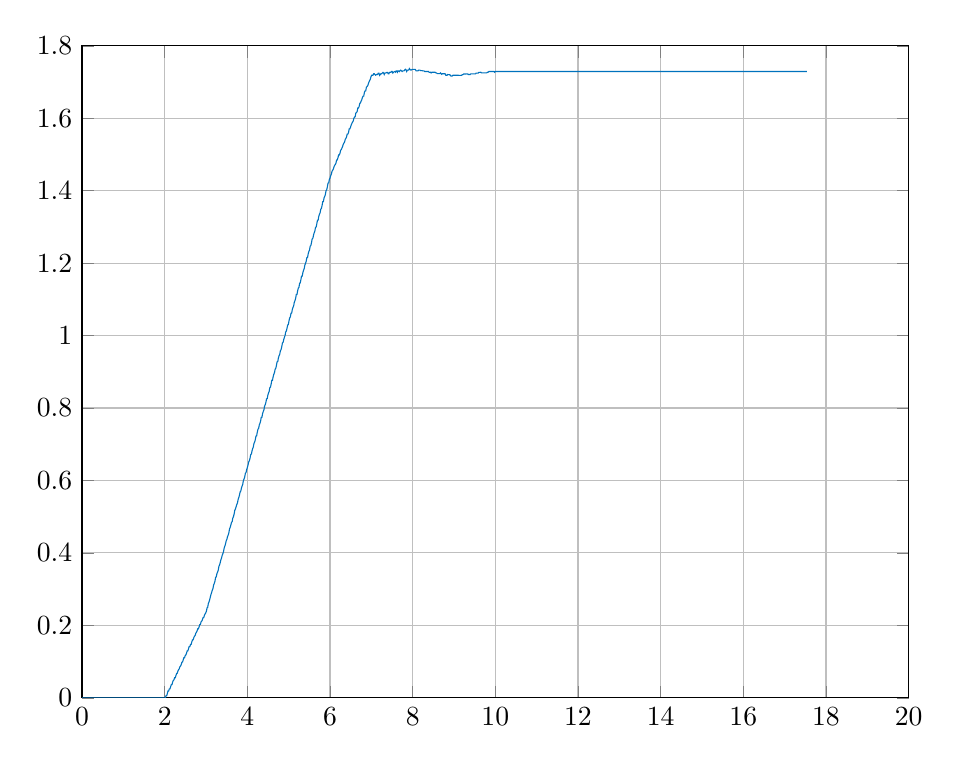
\begin{tikzpicture}

\begin{axis}[%
width=4.133in,
height=3.26in,
at={(0.693in,0.44in)},
scale only axis,
xmin=0,
xmax=20,
xmajorgrids,
ymin=0,
ymax=1.8,
ymajorgrids,
axis background/.style={fill=white}
]
\addplot [color=mycolor1,solid,forget plot]
  table[row sep=crcr]{%
0	0\\
0.0177479479990005	0\\
0.0329936939989999	0\\
0.0481602929999996	0\\
0.0637873389999997	0\\
0.0797200289990008	0\\
0.0957228709999993	0\\
0.111884321	0\\
0.127813586998999	0\\
0.143877488999	0\\
0.159849068999	0\\
0.175815245999999	0\\
0.191849568	0\\
0.207857955999	0\\
0.223800520001	0\\
0.239917723999999	0\\
0.255887639999	0\\
0.271865544	0\\
0.287860586999999	0\\
0.303721629000001	0\\
0.321694859999999	0\\
0.336783476999	0\\
0.352006797	0\\
0.368031238	0\\
0.384027142999999	0\\
0.400025939999999	0\\
0.415768619999999	0\\
0.431827854	0\\
0.447846225	0\\
0.464050762	0\\
0.480125345000999	0\\
0.495960108999999	0\\
0.51223874	0\\
0.528013373	0\\
0.543888207999	0\\
0.559718538000001	0\\
0.577693402000999	0\\
0.593169072000001	0\\
0.608436084999999	0\\
0.624012790999999	0\\
0.639968403999001	0\\
0.655979648999	0\\
0.671886863	0\\
0.687915775	0\\
0.704005574999999	0\\
0.719979369000999	0\\
0.735999127999	0\\
0.751804396	0\\
0.767977141998	0\\
0.784254729	0\\
0.799888649	0\\
0.816014402999001	0\\
0.831968129999	0\\
0.847920805	0\\
0.863995878001001	0\\
0.879922455999	0\\
0.895839980999	0\\
0.912009702	0\\
0.928008587998999	0\\
0.944009664000001	0\\
0.959998357999999	0\\
0.975881722999999	0\\
0.991856344	0\\
1.007854506001	0\\
1.023802485	0\\
1.04204285	0\\
1.057257473	0\\
1.072062135	0\\
1.087877377	0\\
1.103944708	0\\
1.12000716	0\\
1.135921448999	0\\
1.151953203	0\\
1.167871553001	0\\
1.183870008	0\\
1.199982183999	0\\
1.216054860999	0\\
1.232003181999	0\\
1.248082351	0\\
1.264018650999	0\\
1.279993787999	0\\
1.296059125	0\\
1.311952701	0\\
1.327714297	0\\
1.345778612	0\\
1.360896684	0\\
1.376431839	0\\
1.392044326	0\\
1.408126785999	0\\
1.423958204	0\\
1.439964040999	0\\
1.455968049	0\\
1.471994328	0\\
1.488003763	0\\
1.50397653	0\\
1.519928540999	0\\
1.535971151	0\\
1.551950773999	0\\
1.567714147	0\\
1.585839139999	0\\
1.601398660999	0\\
1.616814482	0\\
1.632216331	0\\
1.64800661	0\\
1.664003086	0\\
1.679973443	0\\
1.696057768	0\\
1.712011457	0\\
1.727998195999	0\\
1.744301857999	0\\
1.759866504999	0\\
1.775813906	0\\
1.791863632	0\\
1.807946573999	0\\
1.823762762	0\\
1.839968330999	0\\
1.856014943	0\\
1.872034705	0\\
1.887959407999	0\\
1.904015003001	0\\
1.920010021	0\\
1.936055037	0\\
1.952016794	0\\
1.968015921	0\\
1.984015635	0\\
1.999982228	0\\
2.017637973	0\\
2.033024109	0.0058566180016042\\
2.048360808	0.00585654081512067\\
2.063713924	0.0117127807322883\\
2.079994301001	0.0188739372844323\\
2.09587115	0.0188740459583119\\
2.111858971999	0.0247303997977806\\
2.12786286	0.0247304385082166\\
2.143782009	0.0305865549320426\\
2.16007562	0.0364426401790212\\
2.175995763	0.0364424177326113\\
2.191966860999	0.0436051626650057\\
2.208002772	0.04750864264365\\
2.223843195	0.0494613159269937\\
2.239834443999	0.0553170223164103\\
2.255812463	0.0553170062414349\\
2.271841413	0.0611724892030901\\
2.287860835	0.0670279672435049\\
2.303989108	0.0679030888535418\\
2.321209679	0.0741926232162643\\
2.336562311999	0.0780955833975912\\
2.351939425	0.080047885703275\\
2.367944861	0.0859029861037292\\
2.383875042	0.0878558045053353\\
2.399840187001	0.0917578638675243\\
2.415882334	0.0980574218815325\\
2.431851019	0.0989243513358559\\
2.447854261	0.104779184277435\\
2.464045368	0.110633903460174\\
2.479855647	0.110633899394429\\
2.495984533	0.116488462255225\\
2.51202352	0.118441014303541\\
2.527991351	0.122788006879818\\
2.54388498	0.129510824865517\\
2.56070428	0.129510892923684\\
2.575865885	0.135365220034985\\
2.591992039001	0.141219324235904\\
2.608014273	0.141219235299147\\
2.624008184	0.147073026667943\\
2.64002879	0.147519186637321\\
2.655995271999	0.15424300260169\\
2.67203665	0.160096938985096\\
2.688051693999	0.160096938985096\\
2.703972252	0.165950520422618\\
2.720023863	0.16985223861668\\
2.736053635	0.171803919728936\\
2.751840787	0.178104294207732\\
2.767999686	0.180927904148457\\
2.784001759	0.184829047204358\\
2.799859341	0.190682193097418\\
2.815715874	0.190682193097418\\
2.833736597	0.196535197619143\\
2.849220902001	0.20238815204978\\
2.864796695999	0.202835816138198\\
2.880273093	0.209561535652271\\
2.896046013	0.211513597347654\\
2.912004603	0.215414244283096\\
2.927990109	0.22126685129814\\
2.943974408	0.22126685129814\\
2.959890851999	0.227119170563254\\
2.975972457	0.231468479657371\\
2.992168394	0.233858449471305\\
3.011038520001	0.2401466649391\\
3.023967191	0.247930678062266\\
3.040386992	0.249881900512893\\
3.055854327	0.260576869494562\\
3.071747976999	0.264459838332742\\
3.088006849	0.270760782573689\\
3.104008896	0.278544662048592\\
3.120000907	0.285255270758596\\
3.135988638001	0.291106946329595\\
3.151979592	0.296941991177408\\
3.16799241	0.301800273954533\\
3.184023777999	0.311535065753582\\
3.199988409	0.315868498894426\\
3.216015448999	0.321719871805466\\
3.231996646	0.332332304923145\\
3.247965231999	0.334274906065155\\
3.264002310999	0.343024332764688\\
3.280044226	0.346908002428378\\
3.296262709	0.352758876040755\\
3.311737804	0.36294424408868\\
3.327687419	0.36682793510187\\
3.344040488	0.373557961224096\\
3.360013891998	0.381341924503358\\
3.376044635	0.386191218197453\\
3.391975337	0.393982976523266\\
3.407822791	0.39786697032526\\
3.423851995999	0.404168764269055\\
3.439797332	0.413903153510568\\
3.455802596999	0.418668270918236\\
3.471892084	0.424998772804718\\
3.487888756	0.43325682168546\\
3.504114636	0.437150367670054\\
3.519942030999	0.444941532817147\\
3.536004884	0.449278286711814\\
3.551805854	0.455127998075744\\
3.567770947	0.465744582442496\\
3.583985975	0.470582509417178\\
3.60000599	0.476431987796814\\
3.615853618	0.484215683689801\\
3.632100316	0.486165856026167\\
3.648017793	0.496353095247012\\
3.663964261	0.500238275517594\\
3.680019690999	0.507450000258195\\
3.695977999999	0.517656868448925\\
3.711993644	0.521541876655597\\
3.728395969999	0.527390727371792\\
3.743879563999	0.533680413246373\\
3.759998042	0.537578483375172\\
3.776007270999	0.547312568758965\\
3.791980901	0.552592039487812\\
3.807733244	0.558881869653845\\
3.825688622	0.568615743340341\\
3.840815172	0.570559251932276\\
3.856523527	0.578803987129462\\
3.872035549998	0.584640441313328\\
3.887865093	0.589015190402568\\
3.903864740999	0.59966522867547\\
3.919875002999	0.603992976498663\\
3.935936306	0.609840880567341\\
3.952029105	0.619574749350508\\
3.968017443	0.621973659197642\\
3.98403859	0.629763442438864\\
3.999879734	0.636076738056453\\
4.017293907	0.642833804601234\\
4.032535623	0.651066458574794\\
4.047964042	0.654952815545206\\
4.063895768	0.660800239764456\\
4.079692714	0.670989411676461\\
4.097733388	0.672933235667604\\
4.112779089999	0.681669125817141\\
4.128063351999	0.687951581067076\\
4.143795641	0.692292593449099\\
4.159892966	0.702026581937098\\
4.175874410999	0.705913598297726\\
4.191873398	0.712215020359873\\
4.207789674	0.722424469443861\\
4.223859429	0.722893529660044\\
4.23984077	0.733074258226057\\
4.255914688999	0.741305088909293\\
4.271870471999	0.743252990085705\\
4.287856895	0.752987147418436\\
4.303852883999	0.7573279716268\\
4.319702097	0.763649818518933\\
4.33577652	0.773851812946894\\
4.351891424	0.774299674093377\\
4.3679941	0.784479073162639\\
4.384025651	0.790316449808019\\
4.399910400999	0.79421356286477\\
4.415978467	0.804874970490012\\
4.432017986	0.809229877012757\\
4.448000485	0.81507650670847\\
4.464053399	0.825259565138579\\
4.479980979	0.825705346301158\\
4.495972970001	0.835439929131033\\
4.511980807	0.841277368624594\\
4.527918322	0.846100122906953\\
4.543785381	0.85630114372459\\
4.560817471999	0.858245883565385\\
4.575718425	0.866484997680507\\
4.59201348	0.876666231147318\\
4.60806531	0.876666231147318\\
4.624003596	0.886401259998868\\
4.639986832	0.893162331375195\\
4.655989813	0.897525708925555\\
4.671928117	0.907260454216531\\
4.688016512	0.909654967839208\\
4.703853887	0.917892453843724\\
4.71996996	0.927627417204047\\
4.735997922	0.928549790136689\\
4.751868964	0.938750187241673\\
4.767862568	0.944588055964228\\
4.783818822999	0.948484953460701\\
4.800085902	0.958670380809334\\
4.815731593	0.961063728689615\\
4.831966108998	0.968853902094833\\
4.847975770001	0.979509709657975\\
4.866422204001	0.981919791304468\\
4.881673619	0.989709525663175\\
4.896807591	0.995546951377901\\
4.91192445	0.999895719308199\\
4.927860524	1.01007995508596\\
4.943857179999	1.01249544215504\\
4.959824591	1.02073464803622\\
4.975995943	1.02898562066701\\
4.991981749	1.03093319277208\\
5.007780037	1.04066865072468\\
5.02407568	1.04890820042592\\
5.039952249001	1.0513061124329\\
5.055858844	1.06151164599825\\
5.071785283	1.06196018752015\\
5.088002434	1.07215901438851\\
5.104033445	1.07799829190884\\
5.120036701	1.08189577068393\\
5.135971518001	1.09208356663367\\
5.151948073	1.0964273359874\\
5.167871053001	1.10273814859441\\
5.183875362001	1.11338503405041\\
5.199950867001	1.1133851025915\\
5.215862265	1.12312233168492\\
5.231877784	1.13091073716896\\
5.247917016998	1.13331020009647\\
5.263848381001	1.14396408466946\\
5.279969113	1.14591004479029\\
5.295988267	1.15461033823723\\
5.311712721	1.16434831865781\\
5.327828851	1.164347947005\\
5.343820617999	1.17408626141357\\
5.360076797	1.18037642637769\\
5.376020889999	1.18518937367748\\
5.391981990999	1.19492770848508\\
5.408016142	1.19973063929917\\
5.423995900001	1.20557371653284\\
5.439882317	1.21531200482953\\
5.4559172	1.21576177158259\\
5.471839277	1.22550080601763\\
5.487854431	1.23225434805297\\
5.504041037999	1.23615316132742\\
5.51999614	1.24679851024042\\
5.536030426999	1.24874434590678\\
5.551842044	1.25653775070882\\
5.567730104	1.2667263115209\\
5.585784461	1.26913874046852\\
5.601230233	1.2773779049093\\
5.616702184	1.28367884263594\\
5.632079409	1.28802208440486\\
5.648002391	1.29776256622787\\
5.663964169	1.29970923115149\\
5.679763131	1.30795089020407\\
5.695984523	1.31815692354915\\
5.711895174	1.31860201547919\\
5.727963343	1.32880210676692\\
5.743993235	1.33508713799354\\
5.760002876	1.33898684126966\\
5.775889422999	1.34872824667681\\
5.791881403	1.3511217363084\\
5.808140761	1.35938135986343\\
5.82397346	1.36956727750255\\
5.83992317	1.37002525588129\\
5.856030908	1.38021031403433\\
5.871977601	1.3841072964474\\
5.887992134	1.38995204282418\\
5.903982756	1.40014080872386\\
5.919880332999	1.40255175834746\\
5.936060871	1.41079069738205\\
5.952041506001	1.42099069925268\\
5.96801938	1.42143311614441\\
5.983999730001	1.43117554646585\\
5.999953624999	1.43507294153589\\
6.017621116	1.44182764184808\\
6.032873947001	1.44572024634279\\
6.04850025	1.45351775373341\\
6.063726808	1.45636292549923\\
6.081792935001	1.46025550266047\\
6.096886416	1.46610600633687\\
6.112470293	1.469999037998\\
6.128013237	1.47240875253856\\
6.144019334	1.47630443592535\\
6.159870089	1.48453999000978\\
6.175860287	1.4849960120359\\
6.192023759	1.49083924927107\\
6.207960793	1.49863269693834\\
6.223983072	1.49863269693834\\
6.240035671001	1.50298766739739\\
6.256002033	1.51123090821768\\
6.271975197	1.51363228653536\\
6.288020328	1.51752543033763\\
6.303875327999	1.52186886938948\\
6.319737169	1.52771229748056\\
6.335724672999	1.53160575197846\\
6.351964119001	1.5340168357181\\
6.367971706	1.54181095408943\\
6.384008148999	1.54465532727621\\
6.399996236	1.54855123503009\\
6.41602451	1.55634551311676\\
6.43197004	1.55634551311676\\
6.447859469	1.5606992416856\\
6.463904457999	1.57044405538291\\
6.47999351	1.57088953478624\\
6.496055811999	1.57523722186419\\
6.51184732	1.58108570777525\\
6.527992023999	1.58542465829893\\
6.544118385	1.58931867207036\\
6.55995807	1.59172832668708\\
6.575911876	1.59952308320803\\
6.592245679999	1.60341740586775\\
6.608054330999	1.60387003898301\\
6.623966405	1.61405740651926\\
6.639994900001	1.61600509932255\\
6.655919294	1.61795151961079\\
6.671830996	1.62815571105703\\
6.687991799	1.62815544291161\\
6.703980797999	1.63249542312367\\
6.720028711	1.64074355972456\\
6.735979122	1.64269331563267\\
6.751967279	1.64703042359419\\
6.768079297	1.65092906753287\\
6.783850723	1.65723425338199\\
6.799829577999	1.66112872307603\\
6.81578504	1.66112872307603\\
6.831987389	1.67132625316241\\
6.847900317	1.67566317051125\\
6.863960006001	1.67566291607632\\
6.879970804999	1.68540900227657\\
6.896056939	1.68781453370625\\
6.912017804	1.68976108791619\\
6.927992987	1.69560704629097\\
6.944357572001	1.70040318799053\\
6.959974373	1.70429855491215\\
6.975995665	1.70819751389146\\
6.992037459	1.71494401755995\\
7.007961975	1.71883935269298\\
7.02388921	1.71883935269298\\
7.040023756	1.71883935269298\\
7.055868091	1.72273458591235\\
7.071826882	1.72273458591235\\
7.088005846	1.72034207340709\\
7.104031629	1.71883886204082\\
7.119971848	1.72078625870811\\
7.135807252999	1.72078625870811\\
7.151861035	1.72078537132484\\
7.168001687001	1.72468174455032\\
7.183937831	1.72468174455032\\
7.200010119001	1.7183851384606\\
7.215868547999	1.72078883119353\\
7.231790992999	1.72273638680526\\
7.247860307	1.72273599084285\\
7.263940157	1.72468448904414\\
7.279970499999	1.7266321240391\\
7.29586504	1.72468142029969\\
7.311722655999	1.72078064769222\\
7.327800181999	1.72467749401222\\
7.343863709	1.7251250955514\\
7.360005244001	1.72512467847091\\
7.375873058	1.72663181290774\\
7.391871462999	1.72662923047724\\
7.407945391	1.72272806428022\\
7.423831003001	1.72272806428022\\
7.439915183999	1.72662522540306\\
7.455996057	1.72707778497766\\
7.472028805	1.72707778497766\\
7.487875046	1.72902472730993\\
7.503998629999	1.72902433110926\\
7.520040297999	1.72468073789435\\
7.536027268	1.72663018232405\\
7.551890115	1.72857788477406\\
7.567721665	1.72902390342687\\
7.5861154	1.72707352741295\\
7.60139779	1.73097055852672\\
7.616785247	1.73097014551297\\
7.632220815	1.72706985915856\\
7.647951271	1.73096711451795\\
7.663896174	1.73096676995099\\
7.679996679	1.72902285711126\\
7.696036570001	1.73097253523885\\
7.71214333	1.73291972019614\\
7.727993995	1.73096918974984\\
7.743886445999	1.72901943384173\\
7.759996043	1.73096621287897\\
7.776036133	1.73096621287897\\
7.791939935	1.73096621287897\\
7.807916499999	1.73336051276943\\
7.823798476999	1.7353084583232\\
7.840007785	1.7333579278769\\
7.855912859	1.72901503664309\\
7.871797472	1.73291311777892\\
7.887993023	1.73291311777892\\
7.903952829001	1.7329125010581\\
7.920036790999	1.73726104846872\\
7.935979544999	1.73486776142527\\
7.951981453	1.73291683540217\\
7.968005783	1.73291652825768\\
7.983967796	1.73486526838725\\
7.999905403	1.73486478497092\\
8.016297471	1.73486415746259\\
8.031940138999	1.73486415746259\\
8.047935483	1.73486415746259\\
8.063846514	1.73486351904969\\
8.082104429999	1.7309644006495\\
8.097426131999	1.7309644006495\\
8.112739721	1.73096367295772\\
8.128074086999	1.73096367295772\\
8.143850079	1.73291404897164\\
8.159889943999	1.73291404897164\\
8.175824349	1.7329133104347\\
8.191905639999	1.73140584568797\\
8.207890993	1.73140732238869\\
8.22387234	1.73140649475104\\
8.239851848	1.73095829341002\\
8.255839178	1.73095829341002\\
8.271852802	1.73095779518115\\
8.287854395	1.72900757383726\\
8.30402028	1.72900757383726\\
8.31980412	1.72900815251605\\
8.336011233	1.72900815251605\\
8.352009137	1.72900815251605\\
8.367962107	1.72900755466559\\
8.383944283	1.72900755466559\\
8.400081984	1.72661389594187\\
8.415921980999	1.72661328737874\\
8.431818875	1.72705536313927\\
8.447883216	1.72510591870957\\
8.463850381	1.72705575192142\\
8.479858884	1.72705575192142\\
8.495884777	1.72705590659145\\
8.511995511	1.72705590659145\\
8.528000336	1.72705519870375\\
8.543983181	1.72705519870375\\
8.559821298	1.72510559841607\\
8.575709962999	1.72510480203524\\
8.594123704001	1.72315458069135\\
8.609327226999	1.72315458069135\\
8.624393220001	1.72315377371671\\
8.639904151	1.72315377371671\\
8.655862035	1.72315377371671\\
8.672006787	1.72510333216221\\
8.687992985	1.72315349853297\\
8.703906813	1.72120327718908\\
8.719752428	1.72315290181147\\
8.735837304	1.72315290181147\\
8.751816660999	1.72270810302847\\
8.767782974	1.72270752700072\\
8.783811858	1.72270752700072\\
8.799881896	1.71880731676353\\
8.81572164	1.71880731676353\\
8.831787176	1.71880665267207\\
8.847990869001	1.72075702868599\\
8.863985837999	1.72031359130617\\
8.880016285999	1.72031291675336\\
8.896014445999	1.72031291675336\\
8.912003973001	1.71836269540947\\
8.927823802	1.71641178905145\\
8.943854295	1.71641178905145\\
8.960005256	1.7168545456486\\
8.976364959999	1.71880430325474\\
8.991984136001	1.71880430325474\\
9.007830677	1.71880430325474\\
9.023818483998	1.71880430325474\\
9.039895683	1.71880430325474\\
9.055902773	1.71880379343445\\
9.071852926999	1.71880379343445\\
9.087997856	1.71880379343445\\
9.103964241	1.71880327328519\\
9.120175582	1.71836051668804\\
9.135942132	1.71836051668804\\
9.151918207999	1.71835998620983\\
9.167873094	1.71835998620983\\
9.183864909	1.71835998620983\\
9.199871147	1.72030997584898\\
9.215849197	1.72030997584898\\
9.231858322	1.72226027455759\\
9.248009198	1.72225980054859\\
9.264024361	1.72225980054859\\
9.280026715	1.72225980054859\\
9.295932959999	1.72225980054859\\
9.311729004	1.7227007110213\\
9.327987888999	1.7227007110213\\
9.343968201	1.72075033500738\\
9.359862077	1.72074949975633\\
9.376084164001	1.72074949975633\\
9.392017938	1.72074949975633\\
9.407866846	1.72269949270159\\
9.424000306	1.72269949270159\\
9.439986635	1.72269949270159\\
9.455974396	1.72269871353649\\
9.471997591999	1.72269871353649\\
9.488004372	1.72269871353649\\
9.503898681999	1.72269792391027\\
9.520109253001	1.72269792391027\\
9.535889759	1.72464822261888\\
9.551926410999	1.72464742253159\\
9.567902261999	1.72464742253159\\
9.583865534	1.72464742253159\\
9.600044915	1.72659775778222\\
9.616020525	1.72659775778222\\
9.63199765	1.72659775778222\\
9.647976117999	1.72704085477746\\
9.663990434	1.7250897344058\\
9.67998426	1.7250897344058\\
9.695892676	1.7250897344058\\
9.711893747	1.72508897952763\\
9.727857329001	1.72508897952763\\
9.743905853	1.72508897952763\\
9.759862188	1.72508821412903\\
9.775864115999	1.72508821412903\\
9.791994987	1.72508821412903\\
9.807842721	1.72703889025897\\
9.823815987	1.72703889025897\\
9.842002391998	1.72898918896758\\
9.857432615	1.7289884789421\\
9.872999893	1.7289884789421\\
9.88845594	1.7289884789421\\
9.904112290999	1.72898775833681\\
9.9200017	1.72898775833681\\
9.935996482	1.72898775833681\\
9.952011249	1.72898775833681\\
9.967997131001	1.72898702715175\\
9.983979419999	1.72703665113783\\
9.9998719	1.72898833225009\\
10.017346415	1.72898766672081\\
10.032432738999	1.72898766672081\\
10.047884843999	1.72898766672081\\
10.063804669	1.72898766672081\\
10.079994113	1.72898766672081\\
10.096082874	1.72898766672081\\
10.112146416	1.72898766672081\\
10.128000202999	1.72898766672081\\
10.143989502999	1.72898766672081\\
10.159918174998	1.72898766672081\\
10.175970893999	1.72898766672081\\
10.192046879999	1.72898766672081\\
10.208018284	1.72898766672081\\
10.22400154	1.72898766672081\\
10.239995987	1.72898766672081\\
10.255989396	1.72898766672081\\
10.272045397	1.72898766672081\\
10.288084068999	1.72898766672081\\
10.303975091	1.72898766672081\\
10.319728771	1.72898766672081\\
10.337687306	1.72898766672081\\
10.352930153999	1.72898766672081\\
10.368230414	1.72898766672081\\
10.38390628	1.72898766672081\\
10.400124519	1.72898766672081\\
10.41608605	1.72898766672081\\
10.431875165999	1.72898766672081\\
10.447880458	1.72898766672081\\
10.463861924	1.72898766672081\\
10.479844504	1.72898766672081\\
10.496008834999	1.72898766672081\\
10.512011771	1.72898766672081\\
10.528019808	1.72898766672081\\
10.543855718	1.72898766672081\\
10.559805752	1.72898766672081\\
10.575896981999	1.72898766672081\\
10.591898288	1.72898766672081\\
10.60800516	1.72898766672081\\
10.624021391	1.72898766672081\\
10.639960808	1.72898766672081\\
10.656006254999	1.72898766672081\\
10.671923579001	1.72898766672081\\
10.687916537	1.72898766672081\\
10.703992730999	1.72898766672081\\
10.719996679	1.72898766672081\\
10.736302646999	1.72898766672081\\
10.751984363999	1.72898766672081\\
10.76793415	1.72898766672081\\
10.783899515	1.72898766672081\\
10.799998619	1.72898766672081\\
10.81582196	1.72898766672081\\
10.831704556	1.72898766672081\\
10.848020849	1.72898766672081\\
10.863991553999	1.72898766672081\\
10.880032740999	1.72898766672081\\
10.895978476999	1.72898766672081\\
10.911786188999	1.72898766672081\\
10.927752211001	1.72898766672081\\
10.943863785	1.72898766672081\\
10.959849236	1.72898766672081\\
10.975856089999	1.72898766672081\\
10.991824943999	1.72898766672081\\
11.010578926001	1.72898766672081\\
11.025806075	1.72898766672081\\
11.041347875	1.72898766672081\\
11.056684078	1.72898766672081\\
11.071868932	1.72898766672081\\
11.087990874	1.72898766672081\\
11.103860146999	1.72898766672081\\
11.11975065	1.72898766672081\\
11.135967342	1.72898766672081\\
11.152131372999	1.72898766672081\\
11.168046533	1.72898766672081\\
11.183910372999	1.72898766672081\\
11.200118540999	1.72898766672081\\
11.215869521	1.72898766672081\\
11.231853733998	1.72898766672081\\
11.247861495999	1.72898766672081\\
11.264078662	1.72898766672081\\
11.280040129	1.72898766672081\\
11.295985098001	1.72898766672081\\
11.31193109	1.72898766672081\\
11.327713270001	1.72898766672081\\
11.344012231999	1.72898766672081\\
11.359904011	1.72898766672081\\
11.375858757	1.72898766672081\\
11.391849525	1.72898766672081\\
11.407939417	1.72898766672081\\
11.423860638	1.72898766672081\\
11.439857811	1.72898766672081\\
11.455989412999	1.72898766672081\\
11.471992935	1.72898766672081\\
11.488085133	1.72898766672081\\
11.503960655	1.72898766672081\\
11.519851832999	1.72898766672081\\
11.535856582	1.72898766672081\\
11.551792822001	1.72898766672081\\
11.567726039	1.72898766672081\\
11.585870336	1.72898766672081\\
11.601391025	1.72898766672081\\
11.616884139	1.72898766672081\\
11.632365448	1.72898766672081\\
11.647795521	1.72898766672081\\
11.664067051	1.72898766672081\\
11.680023827	1.72898766672081\\
11.695989188	1.72898766672081\\
11.712051197001	1.72898766672081\\
11.728041229	1.72898766672081\\
11.744160127	1.72898766672081\\
11.759880488	1.72898766672081\\
11.776004678	1.72898766672081\\
11.791973351	1.72898766672081\\
11.807931498	1.72898766672081\\
11.823800660999	1.72898766672081\\
11.839929526	1.72898766672081\\
11.85598562	1.72898766672081\\
11.871950714999	1.72898766672081\\
11.887978206	1.72898766672081\\
11.9040818	1.72898766672081\\
11.920122113	1.72898766672081\\
11.936037713	1.72898766672081\\
11.952065921	1.72898766672081\\
11.968176174998	1.72898766672081\\
11.984088696	1.72898766672081\\
12.000047981999	1.72898766672081\\
12.015760442	1.72898766672081\\
12.031875402	1.72898766672081\\
12.048090962	1.72898766672081\\
12.065227336	1.72898766672081\\
12.080138343	1.72898766672081\\
12.095987001	1.72898766672081\\
12.112005933001	1.72898766672081\\
12.128009998	1.72898766672081\\
12.144042558	1.72898766672081\\
12.159913176999	1.72898766672081\\
12.17599663	1.72898766672081\\
12.191927231999	1.72898766672081\\
12.207876833	1.72898766672081\\
12.223719491	1.72898766672081\\
12.240037539	1.72898766672081\\
12.256067371	1.72898766672081\\
12.272187226	1.72898766672081\\
12.288019225	1.72898766672081\\
12.30416534	1.72898766672081\\
12.319719077001	1.72898766672081\\
12.338075044	1.72898766672081\\
12.353670201	1.72898766672081\\
12.369075001	1.72898766672081\\
12.384441681	1.72898766672081\\
12.400072168	1.72898766672081\\
12.415973738999	1.72898766672081\\
12.431878442	1.72898766672081\\
12.448181763	1.72898766672081\\
12.464014654	1.72898766672081\\
12.479980455	1.72898766672081\\
12.495999775	1.72898766672081\\
12.512070763	1.72898766672081\\
12.527837053001	1.72898766672081\\
12.543842924998	1.72898766672081\\
12.559952958	1.72898766672081\\
12.575711244001	1.72898766672081\\
12.593980047999	1.72898766672081\\
12.609465957	1.72898766672081\\
12.624944328	1.72898766672081\\
12.640197992	1.72898766672081\\
12.655827693999	1.72898766672081\\
12.671855215	1.72898766672081\\
12.687847201	1.72898766672081\\
12.703825676001	1.72898766672081\\
12.719841826	1.72898766672081\\
12.735903656	1.72898766672081\\
12.7519258	1.72898766672081\\
12.767984532	1.72898766672081\\
12.783865582	1.72898766672081\\
12.800110826	1.72898766672081\\
12.815748685001	1.72898766672081\\
12.833787777	1.72898766672081\\
12.848887157	1.72898766672081\\
12.864859869001	1.72898766672081\\
12.880127835	1.72898766672081\\
12.896136238	1.72898766672081\\
12.914398054999	1.72898766672081\\
12.929565729	1.72898766672081\\
12.944687434	1.72898766672081\\
12.960237042	1.72898766672081\\
12.97609728	1.72898766672081\\
12.992053314	1.72898766672081\\
13.009906641998	1.72898766672081\\
13.024986992	1.72898766672081\\
13.040261448	1.72898766672081\\
13.056239738	1.72898766672081\\
13.071759365	1.72898766672081\\
13.087771287	1.72898766672081\\
13.10397946	1.72898766672081\\
13.119829148	1.72898766672081\\
13.135808145	1.72898766672081\\
13.151805989	1.72898766672081\\
13.168001175	1.72898766672081\\
13.184011608	1.72898766672081\\
13.1998695	1.72898766672081\\
13.215891032999	1.72898766672081\\
13.23198076	1.72898766672081\\
13.247892233	1.72898766672081\\
13.263879197999	1.72898766672081\\
13.279861787999	1.72898766672081\\
13.295822988999	1.72898766672081\\
13.311817284	1.72898766672081\\
13.327788268999	1.72898766672081\\
13.343978818999	1.72898766672081\\
13.360002907999	1.72898766672081\\
13.375992086999	1.72898766672081\\
13.392012759	1.72898766672081\\
13.407903117999	1.72898766672081\\
13.423890853	1.72898766672081\\
13.440115938999	1.72898766672081\\
13.456126015	1.72898766672081\\
13.47200261	1.72898766672081\\
13.488005365	1.72898766672081\\
13.504007494	1.72898766672081\\
13.519869235	1.72898766672081\\
13.535859612001	1.72898766672081\\
13.551867965	1.72898766672081\\
13.567927203	1.72898766672081\\
13.583750089	1.72898766672081\\
13.599846965	1.72898766672081\\
13.615896469	1.72898766672081\\
13.632121014	1.72898766672081\\
13.648011524	1.72898766672081\\
13.664011343	1.72898766672081\\
13.679992784999	1.72898766672081\\
13.695996698	1.72898766672081\\
13.711996271	1.72898766672081\\
13.727995604	1.72898766672081\\
13.744035462999	1.72898766672081\\
13.760001664	1.72898766672081\\
13.775991606999	1.72898766672081\\
13.791979899	1.72898766672081\\
13.807884878001	1.72898766672081\\
13.823704098999	1.72898766672081\\
13.839954995	1.72898766672081\\
13.856008876	1.72898766672081\\
13.872138644	1.72898766672081\\
13.887912470001	1.72898766672081\\
13.903863348	1.72898766672081\\
13.919890613999	1.72898766672081\\
13.936002782	1.72898766672081\\
13.951972948999	1.72898766672081\\
13.967873783	1.72898766672081\\
13.98385298	1.72898766672081\\
13.999845186	1.72898766672081\\
14.016277028	1.72898766672081\\
14.031914659	1.72898766672081\\
14.047916188	1.72898766672081\\
14.063810401	1.72898766672081\\
14.079697027999	1.72898766672081\\
14.09765261	1.72898766672081\\
14.113077426	1.72898766672081\\
14.128468190001	1.72898766672081\\
14.144034982	1.72898766672081\\
14.159940973001	1.72898766672081\\
14.175967513001	1.72898766672081\\
14.191979734	1.72898766672081\\
14.207995513999	1.72898766672081\\
14.224122065	1.72898766672081\\
14.239749623	1.72898766672081\\
14.255865817	1.72898766672081\\
14.271905571	1.72898766672081\\
14.287834284	1.72898766672081\\
14.303890711	1.72898766672081\\
14.319836514999	1.72898766672081\\
14.337844106	1.72898766672081\\
14.353238981999	1.72898766672081\\
14.368686184	1.72898766672081\\
14.384164445999	1.72898766672081\\
14.400006988	1.72898766672081\\
14.415987513	1.72898766672081\\
14.431983513	1.72898766672081\\
14.448061879999	1.72898766672081\\
14.463981601	1.72898766672081\\
14.480005221	1.72898766672081\\
14.496037654	1.72898766672081\\
14.512096797	1.72898766672081\\
14.528006844999	1.72898766672081\\
14.543991169	1.72898766672081\\
14.559915141	1.72898766672081\\
14.575707609	1.72898766672081\\
14.593923974	1.72898766672081\\
14.609437240999	1.72898766672081\\
14.625078612	1.72898766672081\\
14.640654745999	1.72898766672081\\
14.656223804	1.72898766672081\\
14.671976068999	1.72898766672081\\
14.688010349	1.72898766672081\\
14.703958726	1.72898766672081\\
14.720018278999	1.72898766672081\\
14.735978613	1.72898766672081\\
14.751898777	1.72898766672081\\
14.767879086	1.72898766672081\\
14.78385257	1.72898766672081\\
14.799888912	1.72898766672081\\
14.815955742	1.72898766672081\\
14.831677953	1.72898766672081\\
14.849750365	1.72898766672081\\
14.864818173	1.72898766672081\\
14.880096476999	1.72898766672081\\
14.895803818	1.72898766672081\\
14.911935785999	1.72898766672081\\
14.928013636	1.72898766672081\\
14.944038216	1.72898766672081\\
14.960024589	1.72898766672081\\
14.975861744	1.72898766672081\\
14.991802669	1.72898766672081\\
15.009049282	1.72898766672081\\
15.02454527	1.72898766672081\\
15.040075114	1.72898766672081\\
15.056167391998	1.72898766672081\\
15.071840964	1.72898766672081\\
15.087758378001	1.72898766672081\\
15.103928547999	1.72898766672081\\
15.120004839	1.72898766672081\\
15.135995993	1.72898766672081\\
15.151899311	1.72898766672081\\
15.167910676	1.72898766672081\\
15.18387206	1.72898766672081\\
15.199869373	1.72898766672081\\
15.216001692	1.72898766672081\\
15.231902396	1.72898766672081\\
15.247851799998	1.72898766672081\\
15.263862874001	1.72898766672081\\
15.279865233	1.72898766672081\\
15.295884421	1.72898766672081\\
15.311874218	1.72898766672081\\
15.327714632	1.72898766672081\\
15.343745821	1.72898766672081\\
15.360000908	1.72898766672081\\
15.375998358998	1.72898766672081\\
15.391840457	1.72898766672081\\
15.407928889999	1.72898766672081\\
15.424070801	1.72898766672081\\
15.440029125	1.72898766672081\\
15.456058501	1.72898766672081\\
15.471853776	1.72898766672081\\
15.487981148	1.72898766672081\\
15.503999448999	1.72898766672081\\
15.519972437001	1.72898766672081\\
15.535889583	1.72898766672081\\
15.55200129	1.72898766672081\\
15.567836566	1.72898766672081\\
15.583773938999	1.72898766672081\\
15.599866671999	1.72898766672081\\
15.615975587999	1.72898766672081\\
15.631887158	1.72898766672081\\
15.647805073999	1.72898766672081\\
15.66400468	1.72898766672081\\
15.680063533	1.72898766672081\\
15.69607999	1.72898766672081\\
15.711999842	1.72898766672081\\
15.728035838	1.72898766672081\\
15.744004846	1.72898766672081\\
15.760038997999	1.72898766672081\\
15.776003717	1.72898766672081\\
15.791975001	1.72898766672081\\
15.808677646999	1.72898766672081\\
15.823890725	1.72898766672081\\
15.839677593	1.72898766672081\\
15.856018254999	1.72898766672081\\
15.872010391	1.72898766672081\\
15.887901072999	1.72898766672081\\
15.903805231999	1.72898766672081\\
15.919870075	1.72898766672081\\
15.935845773999	1.72898766672081\\
15.951943228999	1.72898766672081\\
15.967939879	1.72898766672081\\
15.984084898	1.72898766672081\\
15.999859321	1.72898766672081\\
16.017558313	1.72898766672081\\
16.032743968	1.72898766672081\\
16.047979972	1.72898766672081\\
16.063844965	1.72898766672081\\
16.079758521999	1.72898766672081\\
16.096020761	1.72898766672081\\
16.11187066	1.72898766672081\\
16.128002543	1.72898766672081\\
16.144019826	1.72898766672081\\
16.159890030999	1.72898766672081\\
16.175855823	1.72898766672081\\
16.191869951	1.72898766672081\\
16.207846844999	1.72898766672081\\
16.223979535	1.72898766672081\\
16.239996452	1.72898766672081\\
16.255873056999	1.72898766672081\\
16.27185499	1.72898766672081\\
16.287821333	1.72898766672081\\
16.303975947	1.72898766672081\\
16.319774837	1.72898766672081\\
16.335751282999	1.72898766672081\\
16.351821003001	1.72898766672081\\
16.367848084	1.72898766672081\\
16.383979836001	1.72898766672081\\
16.400007287	1.72898766672081\\
16.415939668	1.72898766672081\\
16.431918901	1.72898766672081\\
16.448046837999	1.72898766672081\\
16.463998664	1.72898766672081\\
16.479873524	1.72898766672081\\
16.495862974	1.72898766672081\\
16.511863679999	1.72898766672081\\
16.527826415	1.72898766672081\\
16.543860376	1.72898766672081\\
16.559870457	1.72898766672081\\
16.575747169999	1.72898766672081\\
16.591999936999	1.72898766672081\\
16.608129336	1.72898766672081\\
16.624000027	1.72898766672081\\
16.639993195	1.72898766672081\\
16.655879692	1.72898766672081\\
16.67186818	1.72898766672081\\
16.687813292	1.72898766672081\\
16.703720532	1.72898766672081\\
16.719796821	1.72898766672081\\
16.735808306	1.72898766672081\\
16.751973935	1.72898766672081\\
16.767973599	1.72898766672081\\
16.783993231999	1.72898766672081\\
16.799871811	1.72898766672081\\
16.815881922999	1.72898766672081\\
16.831720703	1.72898766672081\\
16.847849087	1.72898766672081\\
16.864006497	1.72898766672081\\
16.880164895	1.72898766672081\\
16.89600849	1.72898766672081\\
16.912005181	1.72898766672081\\
16.927914566	1.72898766672081\\
16.943973301999	1.72898766672081\\
16.959975139999	1.72898766672081\\
16.975937754	1.72898766672081\\
16.992155582	1.72898766672081\\
17.007827598	1.72898766672081\\
17.023864878001	1.72898766672081\\
17.039985424	1.72898766672081\\
17.055879653	1.72898766672081\\
17.071984318999	1.72898766672081\\
17.087714796	1.72898766672081\\
17.103898889	1.72898766672081\\
17.119880600999	1.72898766672081\\
17.135892282	1.72898766672081\\
17.151881877	1.72898766672081\\
17.167886285999	1.72898766672081\\
17.183879535	1.72898766672081\\
17.199851571	1.72898766672081\\
17.215779762	1.72898766672081\\
17.231875764	1.72898766672081\\
17.247883013999	1.72898766672081\\
17.263909192	1.72898766672081\\
17.27985545	1.72898766672081\\
17.295859808	1.72898766672081\\
17.311877222	1.72898766672081\\
17.327727820999	1.72898766672081\\
17.346023719	1.72898766672081\\
17.361568395	1.72898766672081\\
17.377021716	1.72898766672081\\
17.392497572	1.72898766672081\\
17.407995908	1.72898766672081\\
17.424017146999	1.72898766672081\\
17.440177414001	1.72898766672081\\
17.456013386	1.72898766672081\\
17.471972368	1.72898766672081\\
17.488158674	1.72898766672081\\
17.504062304999	1.72898766672081\\
17.520037066	1.72898766672081\\
17.535860009	1.72898766672081\\
};
\end{axis}
\end{tikzpicture}%}
      \caption{The error in displacement of the robot over time for
        $(K_{\Psi}^R, K_{\omega}^T) \equiv (0.5 K_{\Psi, max}^R, 0.75 K_{\omega, max}^T)$}
      \label{fig:19_12_distance}
    \end{figure}
  \end{minipage}
  \hfill
  \begin{minipage}{0.45\linewidth}
    \begin{figure}[H]
      \scalebox{0.6}{% This file was created by matlab2tikz.
%
%The latest updates can be retrieved from
%  http://www.mathworks.com/matlabcentral/fileexchange/22022-matlab2tikz-matlab2tikz
%where you can also make suggestions and rate matlab2tikz.
%
\definecolor{mycolor1}{rgb}{0.00000,0.44700,0.74100}%
%
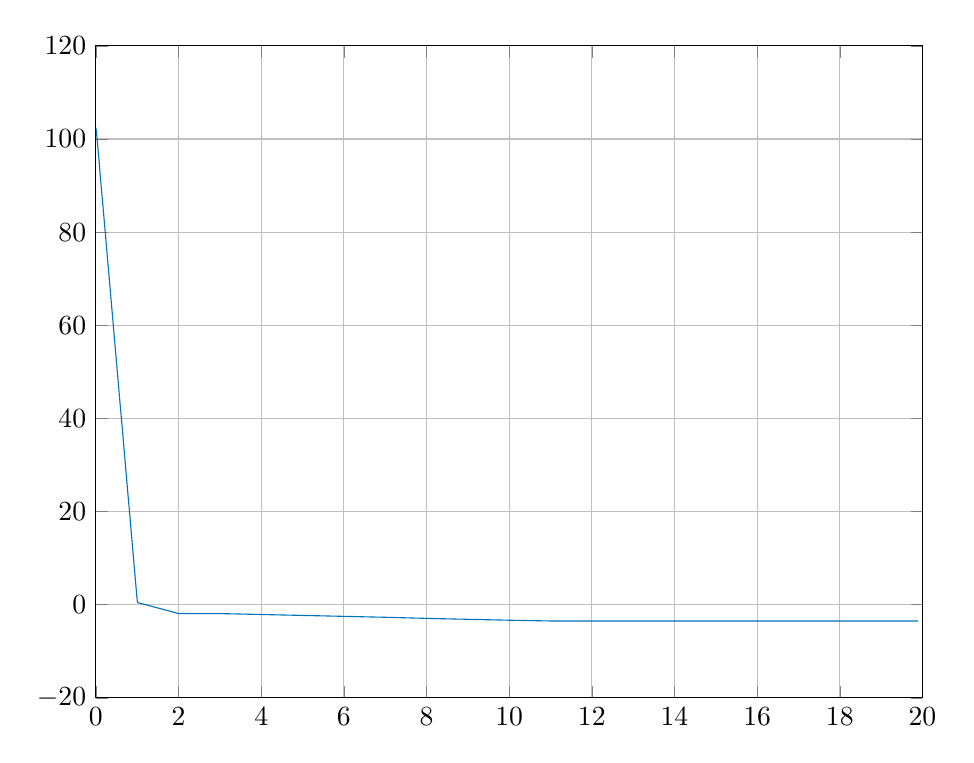
\begin{tikzpicture}

\begin{axis}[%
width=4.133in,
height=3.26in,
at={(0.693in,0.44in)},
scale only axis,
xmin=0,
xmax=20,
xmajorgrids,
ymin=-20,
ymax=120,
ymajorgrids,
axis background/.style={fill=white}
]
\addplot [color=mycolor1,solid,forget plot]
  table[row sep=crcr]{%
0	102.4204\\
0.0149886490000002	101.3744\\
0.0305596550009996	99.9024\\
0.0465867040010002	98.2804\\
0.0648736260019988	96.5744\\
0.0798247719999999	95.0044\\
0.0949272640019991	93.3524\\
0.110540560001999	91.6304\\
0.126725991000999	90.0644\\
0.142763784001	88.4624\\
0.158701440003	86.8824\\
0.174600095000999	85.2644\\
0.190645939001	83.6364\\
0.206556398001	81.9884\\
0.222652333001999	80.3644\\
0.238785739	78.7244\\
0.254748967000999	77.0844\\
0.270559447999999	75.4204\\
0.286598641999999	73.7864\\
0.302760816002	72.1724\\
0.318595918001	70.5284\\
0.334659782002	68.9124\\
0.350533950000999	67.2704\\
0.366668410001999	65.6104\\
0.382531638000999	63.9964\\
0.398638479001999	62.3744\\
0.414560475002	60.7364\\
0.430661805	59.0824\\
0.446547809001999	57.4324\\
0.462549485001	55.8004\\
0.478692660999	54.1804\\
0.494715228000998	52.5464\\
0.510750687001999	50.9064\\
0.526783079001	49.2744\\
0.542723070001999	47.6084\\
0.558590991000999	46.0004\\
0.574902255000999	44.2444\\
0.590520560001999	42.6724\\
0.606775382999999	41.0844\\
0.622569470000999	39.4504\\
0.641072386001999	37.7624\\
0.656406896	36.1344\\
0.671637761001999	34.5164\\
0.686770867000999	32.9044\\
0.702597474001	31.2744\\
0.718692965	29.6404\\
0.734625034001	28.0084\\
0.75082041	26.2504\\
0.766771418001	24.6264\\
0.782720456000999	23.0284\\
0.798574188002	21.4264\\
0.817086090002	19.7564\\
0.832341175000999	18.1284\\
0.847657168001	16.4484\\
0.862952880000999	14.8404\\
0.878763900001999	13.2184\\
0.894750658001	11.6064\\
0.910636666000999	9.99039999999999\\
0.926640575001	8.30439999999999\\
0.942766755000999	6.69039999999998\\
0.958706512001	5.0624\\
0.974582985999999	3.43839999999997\\
0.990674421001999	1.8184\\
1.008171556002	0.450399999999973\\
1.023358636002	0.418399999999991\\
1.038563848002	0.38039999999998\\
1.054602995001	0.346400000000003\\
1.070594481001	0.306399999999996\\
1.086671070002	0.2684\\
1.102760875002	0.228399999999993\\
1.118632451	0.186399999999992\\
1.13456226	0.1524\\
1.150549185002	0.116399999999999\\
1.166737305	0.078400000000002\\
1.182677785	0.0383999999999958\\
1.198574266001	0.000399999999984857\\
1.214567225002	-0.0356000000000023\\
1.230683908001	-0.0736000000000132\\
1.248760177002	-0.113600000000019\\
1.263883792002	-0.151600000000002\\
1.279204980002	-0.187600000000003\\
1.294607131001	-0.22760000000001\\
1.310709859001	-0.261600000000016\\
1.326616108002	-0.301600000000008\\
1.342655634001	-0.3416\\
1.358819683001	-0.379600000000011\\
1.374702561001	-0.417599999999993\\
1.390538120001	-0.451599999999985\\
1.406547556002	-0.49160000000002\\
1.424999306002	-0.533600000000007\\
1.440177833	-0.571600000000018\\
1.455414919001	-0.607600000000005\\
1.470747099001	-0.643600000000021\\
1.486833398001	-0.681600000000003\\
1.502754425001	-0.723600000000005\\
1.518758779001	-0.759600000000006\\
1.534598976999	-0.797600000000017\\
1.550575487002	-0.835599999999999\\
1.566643756001	-0.87360000000001\\
1.582581604	-0.913600000000002\\
1.598525834002	-0.94959999999999\\
1.61477248	-0.989600000000024\\
1.630618046	-1.02560000000001\\
1.646685506001	-1.06160000000003\\
1.662638344	-1.1036\\
1.678742471001	-1.1416\\
1.694618133001	-1.17760000000001\\
1.710706230002	-1.2136\\
1.726581315001	-1.25360000000001\\
1.743942439001	-1.2936\\
1.759150497002	-1.33160000000001\\
1.774746265001	-1.36960000000002\\
1.790620272001	-1.40560000000001\\
1.806658567002	-1.44159999999999\\
1.82273692	-1.4816\\
1.838561571001	-1.52160000000001\\
1.854669635	-1.55960000000002\\
1.870512018002	-1.59760000000001\\
1.886510962	-1.63160000000001\\
1.902563743002	-1.67360000000001\\
1.918651237	-1.7136\\
1.934732152001	-1.74960000000002\\
1.950654199	-1.7856\\
1.966726213001	-1.82360000000001\\
1.982703216002	-1.86560000000001\\
1.998627616001	-1.9016\\
2.014504889002	-1.9156\\
2.032729900002	-1.9156\\
2.047737542	-1.9156\\
2.062772779001	-1.9156\\
2.078712703001	-1.9156\\
2.094694601002	-1.9156\\
2.110538631003	-1.9156\\
2.126537185002	-1.9156\\
2.142558045	-1.9156\\
2.158705649002	-1.9156\\
2.174692087002	-1.9156\\
2.190517009001	-1.9156\\
2.206781121	-1.9156\\
2.222611659002	-1.9156\\
2.238626661001	-1.9156\\
2.254689678002	-1.9156\\
2.270740156	-1.9156\\
2.286748293001	-1.9156\\
2.302640837002	-1.9156\\
2.318700976002	-1.9156\\
2.334581857001	-1.9156\\
2.35072766	-1.9156\\
2.366663663002	-1.9156\\
2.382706469	-1.9156\\
2.398697692002	-1.9156\\
2.414610671	-1.9156\\
2.430576637001	-1.9156\\
2.446557753002	-1.9156\\
2.464792348002	-1.9156\\
2.479917579001	-1.9156\\
2.495223829001	-1.9156\\
2.510543847	-1.9156\\
2.526669781	-1.9156\\
2.542645745001	-1.9156\\
2.558641433003	-1.9156\\
2.575198174	-1.9156\\
2.590658941002	-1.9156\\
2.606734504002	-1.9156\\
2.622577037001	-1.9156\\
2.638546572001	-1.9156\\
2.654696614	-1.9156\\
2.670749898001	-1.9156\\
2.686534622002	-1.9156\\
2.702699809002	-1.9156\\
2.718696988001	-1.9156\\
2.734586834	-1.9156\\
2.750695132002	-1.9156\\
2.766725534001	-1.9156\\
2.782785158001	-1.9156\\
2.798618746002	-1.9156\\
2.814583191002	-1.9156\\
2.830740623001	-1.9156\\
2.846859424002	-1.9156\\
2.862649842001	-1.9156\\
2.878653438	-1.9156\\
2.895526238001	-1.9156\\
2.910744471001	-1.9156\\
2.926637657	-1.9156\\
2.942840261002	-1.9156\\
2.958712038	-1.9156\\
2.974741699	-1.9156\\
2.990640770001	-1.9156\\
3.007965036001	-1.91959999999999\\
3.022965256003	-1.91959999999999\\
3.038826053002	-1.91959999999999\\
3.054570065001	-1.92760000000001\\
3.070616456001	-1.92960000000001\\
3.08654909	-1.92960000000001\\
3.102810662001	-1.9376\\
3.118702634001	-1.9396\\
3.135748349001	-1.9396\\
3.150981194	-1.94359999999999\\
3.166741195002	-1.94959999999999\\
3.182520539	-1.94959999999999\\
3.198532549002	-1.95159999999998\\
3.214663298	-1.95959999999999\\
3.230576133001	-1.95959999999999\\
3.248778240002	-1.9616\\
3.264177301001	-1.96960000000001\\
3.279406914002	-1.96960000000001\\
3.294701851002	-1.96960000000001\\
3.310684309002	-1.97760000000001\\
3.326561172001	-1.9796\\
3.342763486	-1.9796\\
3.359419910002	-1.9876\\
3.375937932001	-1.98960000000002\\
3.391099503	-1.98960000000002\\
3.406697687	-1.99560000000001\\
3.422618973	-1.99960000000002\\
3.438604911001	-1.99960000000002\\
3.454535122002	-2.0056\\
3.470527615	-2.00960000000002\\
3.488914988001	-2.00960000000002\\
3.504056240002	-2.01360000000003\\
3.519064345001	-2.01960000000001\\
3.534803461001	-2.01960000000001\\
3.550604640001	-2.02160000000001\\
3.566976652001	-2.0296\\
3.582686849001	-2.0296\\
3.598758572001	-2.0296\\
3.614729806002	-2.0376\\
3.630530078001	-2.03959999999999\\
3.646594611	-2.03959999999999\\
3.662595559002	-2.04759999999999\\
3.678787369002	-2.04960000000001\\
3.694676740002	-2.04960000000001\\
3.710664267002	-2.05760000000001\\
3.726584927002	-2.0596\\
3.742637831001	-2.0596\\
3.758667424002	-2.06560000000002\\
3.774637822001	-2.06960000000001\\
3.790703357002	-2.06960000000001\\
3.806690968001	-2.07360000000001\\
3.822679932001	-2.0796\\
3.838745079001	-2.0796\\
3.854617855002	-2.08160000000001\\
3.870698278002	-2.08959999999999\\
3.886677698	-2.08959999999999\\
3.90255175	-2.08959999999999\\
3.918555412001	-2.09960000000001\\
3.934904978001	-2.09960000000001\\
3.950567436001	-2.09960000000001\\
3.968828574	-2.10760000000001\\
3.984071857001	-2.10960000000003\\
3.999128773001	-2.10960000000003\\
4.014561097	-2.11760000000001\\
4.030551389	-2.11960000000002\\
4.046554179001	-2.11960000000002\\
4.064719277002	-2.12560000000001\\
4.079732145003	-2.12960000000001\\
4.094820912001	-2.12960000000001\\
4.110752424	-2.1356\\
4.126550204001	-2.1396\\
4.142599233002	-2.1396\\
4.158589209002	-2.14160000000001\\
4.174521342001	-2.14960000000001\\
4.190710944	-2.14960000000001\\
4.206624600001	-2.1516\\
4.222613687	-2.1596\\
4.238711412003	-2.1596\\
4.254692218002	-2.1596\\
4.270901793001	-2.16759999999999\\
4.287127670002	-2.16959999999999\\
4.303276373001	-2.16959999999999\\
4.319268603001	-2.17760000000001\\
4.334692796002	-2.17960000000001\\
4.351335414	-2.17960000000001\\
4.366725607001	-2.18559999999999\\
4.382638739	-2.1896\\
4.398721850001	-2.1896\\
4.414594548	-2.19559999999998\\
4.430565445	-2.19959999999999\\
4.446632283001	-2.19959999999999\\
4.462721433001	-2.20159999999998\\
4.478566408001	-2.20959999999999\\
4.494688415001	-2.20959999999999\\
4.510659077002	-2.2116\\
4.526549456001	-2.21960000000001\\
4.542700242001	-2.21960000000001\\
4.558693255001	-2.21960000000001\\
4.574597732001	-2.2296\\
4.590912084002	-2.2296\\
4.606616158001	-2.2296\\
4.622556083002	-2.2376\\
4.638526474001	-2.23960000000002\\
4.654631880001	-2.23960000000002\\
4.670656495001	-2.24760000000001\\
4.686523361002	-2.24960000000002\\
4.702700849001	-2.24960000000002\\
4.718536837002	-2.2556\\
4.734816527001	-2.25960000000002\\
4.750836059	-2.25960000000002\\
4.766806600001	-2.26560000000002\\
4.782638498001	-2.26960000000001\\
4.798804445	-2.26960000000001\\
4.814684950001	-2.27360000000002\\
4.830571787001	-2.2796\\
4.846737671	-2.2796\\
4.862593698002	-2.2816\\
4.878576162001	-2.28959999999999\\
4.894560792	-2.28959999999999\\
4.910537135	-2.28959999999999\\
4.926506056002	-2.29759999999999\\
4.942553179001	-2.29960000000001\\
4.958683054001	-2.29960000000001\\
4.974700339001	-2.30760000000001\\
4.990592585001	-2.3096\\
5.008011955002	-2.3096\\
5.023058397001	-2.31760000000001\\
5.038643306	-2.31960000000001\\
5.054548472002	-2.31960000000001\\
5.070595439001	-2.3276\\
5.086578314001	-2.3296\\
5.102700486002	-2.3296\\
5.118607880001	-2.3356\\
5.134741341002	-2.33959999999999\\
5.150732114	-2.33959999999999\\
5.166740418001	-2.3416\\
5.182681129	-2.34960000000001\\
5.198587614002	-2.34960000000001\\
5.214627558001	-2.34960000000001\\
5.230582619002	-2.35960000000003\\
5.246707192002	-2.35960000000003\\
5.262568827002	-2.35960000000003\\
5.278616563002	-2.36760000000001\\
5.294560309002	-2.36960000000002\\
5.310562429001	-2.36960000000002\\
5.326700419001	-2.3776\\
5.342679515001	-2.37960000000001\\
5.358564606001	-2.37960000000001\\
5.374655432001	-2.3856\\
5.390698132	-2.3896\\
5.406642384001	-2.3896\\
5.422643475001	-2.39560000000002\\
5.438681755001	-2.39960000000001\\
5.454769182001	-2.39960000000001\\
5.470759303002	-2.4016\\
5.486543300001	-2.4096\\
5.502569969	-2.4096\\
5.518534989	-2.41159999999999\\
5.534566099001	-2.41959999999999\\
5.550634983	-2.41959999999999\\
5.566673549	-2.41959999999999\\
5.582690485001	-2.42960000000001\\
5.598657284002	-2.42960000000001\\
5.614643281	-2.42960000000001\\
5.630667123001	-2.4376\\
5.646630759001	-2.4396\\
5.662629640001	-2.4396\\
5.678668336001	-2.44559999999998\\
5.694799381003	-2.44959999999999\\
5.71093659	-2.44959999999999\\
5.726733539002	-2.45559999999998\\
5.742650088001	-2.45959999999999\\
5.758782049999	-2.45959999999999\\
5.774800746	-2.4636\\
5.790774766003	-2.46960000000001\\
5.806777851	-2.46960000000001\\
5.822830444	-2.47160000000001\\
5.838663073	-2.4796\\
5.854641668001	-2.4796\\
5.870647770001	-2.4796\\
5.886629597	-2.48960000000002\\
5.902723203001	-2.48960000000002\\
5.918631814001	-2.48960000000002\\
5.934789881003	-2.49760000000001\\
5.950733100001	-2.49960000000002\\
5.966701788	-2.49960000000002\\
5.982717671002	-2.5076\\
5.998775806	-2.50960000000002\\
6.014573850001	-2.50960000000002\\
6.03285084	-2.51560000000002\\
6.047993089001	-2.51960000000001\\
6.062955178002	-2.51960000000001\\
6.078578036001	-2.52560000000001\\
6.094584785	-2.5296\\
6.110671281	-2.5296\\
6.126673365002	-2.5316\\
6.142713712002	-2.53959999999999\\
6.1585655	-2.53959999999999\\
6.174521263001	-2.54159999999999\\
6.190687057001	-2.54960000000001\\
6.206497815003	-2.54960000000001\\
6.222634749001	-2.54960000000001\\
6.238526377003	-2.55760000000001\\
6.254699433001	-2.5596\\
6.270868871002	-2.5596\\
6.286561801001	-2.56760000000001\\
6.304824693001	-2.56960000000001\\
6.319802139	-2.56960000000001\\
6.335165647001	-2.57560000000001\\
6.350788295	-2.5796\\
6.366526811001	-2.5796\\
6.384919258001	-2.5856\\
6.400150011999	-2.58959999999999\\
6.415527690001	-2.58959999999999\\
6.430766187002	-2.5936\\
6.446518654001	-2.59960000000001\\
6.462763772001	-2.59960000000001\\
6.478742403	-2.6016\\
6.494719875	-2.60960000000003\\
6.510740385	-2.60960000000003\\
6.526755027001	-2.60960000000003\\
6.542798141001	-2.61960000000002\\
6.558621485003	-2.61960000000002\\
6.574791430002	-2.61960000000002\\
6.590598588001	-2.6276\\
6.606738916001	-2.62960000000001\\
6.622834051001	-2.62960000000001\\
6.638673748001	-2.63759999999999\\
6.654816998001	-2.6396\\
6.670627289002	-2.6396\\
6.686814721001	-2.64560000000002\\
6.703003623001	-2.64960000000001\\
6.718510975002	-2.64960000000001\\
6.734731082001	-2.65560000000001\\
6.750665516001	-2.6596\\
6.766806810002	-2.6596\\
6.782782413	-2.66159999999999\\
6.798526838001	-2.66959999999999\\
6.817021988001	-2.66959999999999\\
6.832092954001	-2.67159999999998\\
6.847590819	-2.67960000000001\\
6.862831328001	-2.67960000000001\\
6.878554924002	-2.67960000000001\\
6.894605661001	-2.6876\\
6.910656172001	-2.6896\\
6.926751108	-2.6896\\
6.942962298	-2.69759999999999\\
6.958630722	-2.69959999999999\\
6.974709183001	-2.69959999999999\\
6.990624200001	-2.7076\\
7.008093739	-2.70959999999999\\
7.023102705	-2.71160000000002\\
7.038715724001	-2.71760000000002\\
7.054592275002	-2.72160000000001\\
7.070599801001	-2.72160000000001\\
7.088854918001	-2.72760000000001\\
7.104052926001	-2.7336\\
7.119112453001	-2.7336\\
7.134556276001	-2.7376\\
7.150633542	-2.74560000000001\\
7.166732867003	-2.74560000000001\\
7.182578709002	-2.74760000000001\\
7.198595302	-2.7556\\
7.214792904001	-2.7576\\
7.230780805002	-2.75960000000001\\
7.246979583	-2.76560000000002\\
7.262582592001	-2.76960000000001\\
7.278628313999	-2.77160000000001\\
7.294809077002	-2.77760000000001\\
7.310703732001	-2.7816\\
7.326704843001	-2.78360000000001\\
7.342562889	-2.78959999999999\\
7.358662574001	-2.79360000000001\\
7.374700283001	-2.79560000000001\\
7.390665398001	-2.80160000000001\\
7.406660684002	-2.8056\\
7.422626393	-2.8056\\
7.438737040001	-2.8096\\
7.454772233002	-2.8176\\
7.470515665001	-2.8176\\
7.486668435002	-2.82159999999999\\
7.502643150002	-2.8296\\
7.518737431999	-2.8296\\
7.534711763003	-2.83160000000001\\
7.550720262001	-2.83759999999999\\
7.566684723002	-2.8416\\
7.582614875	-2.8436\\
7.598629861002	-2.84959999999998\\
7.614589342001	-2.8536\\
7.630652880001	-2.85560000000001\\
7.646613037001	-2.8616\\
7.662700393999	-2.86560000000001\\
7.678561315001	-2.86760000000001\\
7.694559431	-2.87360000000001\\
7.710603984001	-2.8776\\
7.726720445	-2.8776\\
7.742605790001	-2.8836\\
7.758582801001	-2.88960000000002\\
7.774513493002	-2.88960000000002\\
7.790717745001	-2.89360000000002\\
7.806811271002	-2.9016\\
7.822585440001	-2.9016\\
7.838706722002	-2.90360000000001\\
7.854673935002	-2.91159999999999\\
7.870554479002	-2.9136\\
7.886663546002	-2.9156\\
7.902789649002	-2.92160000000001\\
7.918710997002	-2.9256\\
7.934573489	-2.92760000000001\\
7.950658816	-2.9336\\
7.966796804001	-2.9376\\
7.982745548002	-2.93960000000001\\
7.998746378	-2.94560000000001\\
8.014593459002	-2.9496\\
8.030579844002	-2.9496\\
8.046670573	-2.9556\\
8.062574646002	-2.95959999999999\\
8.078798966002	-2.95959999999999\\
8.094717409001	-2.9636\\
8.110734541001	-2.96960000000001\\
8.126509431002	-2.96960000000001\\
8.144769076	-2.97160000000001\\
8.159955674002	-2.97760000000001\\
8.175130492001	-2.9796\\
8.190710233002	-2.9796\\
8.206549660999	-2.98560000000001\\
8.222629724001	-2.9896\\
8.238774258	-2.9896\\
8.25470939	-2.9956\\
8.270750727001	-2.99959999999999\\
8.286690554001	-2.99959999999999\\
8.302621410002	-3.0056\\
8.318677060002	-3.00960000000001\\
8.334783640001	-3.00960000000001\\
8.350744081001	-3.01560000000002\\
8.366713588001	-3.01960000000001\\
8.383025137001	-3.01960000000001\\
8.398690474001	-3.02360000000002\\
8.414711559002	-3.0296\\
8.430685521	-3.0296\\
8.446516277001	-3.0316\\
8.464844528	-3.03959999999999\\
8.479875248001	-3.03959999999999\\
8.495517086001	-3.04159999999999\\
8.510656256001	-3.04759999999999\\
8.526958272	-3.04960000000001\\
8.542689223002	-3.04960000000001\\
8.558627481001	-3.0556\\
8.574532993	-3.05960000000002\\
8.590713014002	-3.05960000000002\\
8.606557583	-3.06560000000002\\
8.622536065001	-3.06960000000001\\
8.638614616001	-3.06960000000001\\
8.654693278002	-3.07560000000001\\
8.670761566	-3.0796\\
8.68658084	-3.0796\\
8.703317317002	-3.0856\\
8.718739692002	-3.08959999999999\\
8.734686960001	-3.08959999999999\\
8.750781487002	-3.0916\\
8.766812203001	-3.09960000000001\\
8.782747398001	-3.09960000000001\\
8.798543078001	-3.1016\\
8.814617943001	-3.10760000000001\\
8.830480673	-3.1096\\
8.846584413002	-3.1096\\
8.862513928	-3.11560000000001\\
8.878552360001	-3.11960000000002\\
8.894636042	-3.11960000000002\\
8.910567833	-3.12560000000001\\
8.926623689001	-3.12960000000001\\
8.942516790001	-3.12960000000001\\
8.958692431002	-3.1356\\
8.974656309	-3.13960000000002\\
8.990676471001	-3.13960000000002\\
9.008138784001	-3.14560000000002\\
9.023149994002	-3.14960000000001\\
9.038608673	-3.14960000000001\\
9.054614495001	-3.15360000000001\\
9.070661940001	-3.1596\\
9.086713369002	-3.1596\\
9.102812528002	-3.16159999999999\\
9.118593856001	-3.16959999999999\\
9.134655405001	-3.16959999999999\\
9.150520211001	-3.16959999999999\\
9.166482863001	-3.17760000000001\\
9.182888112002	-3.17960000000001\\
9.198711299002	-3.17960000000001\\
9.214671035999	-3.18559999999999\\
9.230593081001	-3.18960000000001\\
9.24652732	-3.18960000000001\\
9.262743245001	-3.19560000000001\\
9.278607640001	-3.1996\\
9.294543052	-3.1996\\
9.310527806002	-3.2056\\
9.326560664	-3.20959999999999\\
9.342511293001	-3.20959999999999\\
9.358588505001	-3.21560000000002\\
9.37467926	-3.21960000000001\\
9.390718887001	-3.21960000000001\\
9.406658009001	-3.22160000000001\\
9.422610056999	-3.2296\\
9.438509370001	-3.2296\\
9.454679013001	-3.2316\\
9.470629167999	-3.2376\\
9.486691980002	-3.2396\\
9.502725332001	-3.2396\\
9.518702928002	-3.2456\\
9.534856700001	-3.24959999999999\\
9.550550006001	-3.24959999999999\\
9.566474621	-3.2556\\
9.582636299002	-3.25960000000001\\
9.60104057	-3.25960000000001\\
9.614766618002	-3.26560000000002\\
9.63135709	-3.26960000000001\\
9.646719137001	-3.26960000000001\\
9.662554108002	-3.27560000000001\\
9.678596799	-3.2796\\
9.694754131001	-3.2796\\
9.710888475001	-3.28360000000001\\
9.726601302	-3.28959999999999\\
9.742571087002	-3.28959999999999\\
9.758668488001	-3.2936\\
9.774744697001	-3.29960000000001\\
9.790552465	-3.29960000000001\\
9.806919615002	-3.29960000000001\\
9.822608758001	-3.30760000000001\\
9.838541658001	-3.30960000000002\\
9.854726669001	-3.30960000000002\\
9.870695997002	-3.31560000000002\\
9.88657509	-3.31960000000001\\
9.902668310002	-3.31960000000001\\
9.918562273001	-3.32560000000001\\
9.934684585001	-3.3296\\
9.950699582003	-3.3296\\
9.966662136002	-3.3356\\
9.982682395001	-3.33959999999999\\
9.998642729002	-3.33959999999999\\
10.016064772001	-3.3436\\
10.031107547001	-3.34559999999999\\
10.046791000002	-3.34759999999999\\
10.062802707001	-3.34959999999998\\
10.078620390001	-3.35360000000003\\
10.094538282002	-3.35560000000002\\
10.110545724001	-3.35760000000002\\
10.126518607001	-3.36160000000002\\
10.144785641001	-3.36360000000002\\
10.160056878	-3.36560000000001\\
10.175218121	-3.36960000000002\\
10.190614686001	-3.36960000000002\\
10.206611684	-3.37160000000002\\
10.222752280001	-3.3776\\
10.238697841	-3.3776\\
10.254735745001	-3.37960000000001\\
10.270678497	-3.38560000000003\\
10.286885640001	-3.38560000000003\\
10.302635279001	-3.38760000000002\\
10.318699550001	-3.39160000000001\\
10.334571167999	-3.39360000000002\\
10.350715282002	-3.39560000000002\\
10.366533702002	-3.39760000000001\\
10.382596851002	-3.4016\\
10.398609152001	-3.40360000000001\\
10.414518109001	-3.40560000000001\\
10.430517036001	-3.4096\\
10.448812752001	-3.41159999999999\\
10.464073650002	-3.4136\\
10.479362275002	-3.41760000000002\\
10.494737298	-3.41760000000002\\
10.510645255001	-3.41960000000002\\
10.526661652001	-3.4256\\
10.542557705002	-3.4256\\
10.558634594999	-3.42760000000001\\
10.574824234001	-3.4336\\
10.590677646	-3.4336\\
10.606715743002	-3.43559999999999\\
10.622694053	-3.4396\\
10.638564738001	-3.44159999999999\\
10.654654656	-3.44359999999999\\
10.670656213001	-3.44759999999999\\
10.686600423	-3.44959999999999\\
10.702754907002	-3.45160000000001\\
10.718806112	-3.45360000000002\\
10.734639480002	-3.45760000000003\\
10.750687514002	-3.45960000000002\\
10.766635829001	-3.46160000000002\\
10.782760782002	-3.46560000000002\\
10.79861407	-3.46560000000002\\
10.814787546002	-3.46760000000002\\
10.830756112002	-3.4736\\
10.846677632	-3.4736\\
10.862531825001	-3.47560000000001\\
10.878720286001	-3.48160000000003\\
10.894514471001	-3.48160000000003\\
10.910934283001	-3.48360000000002\\
10.926597165001	-3.48960000000002\\
10.942835379999	-3.48960000000002\\
10.958565892	-3.49160000000002\\
10.974583890001	-3.49560000000001\\
10.990600037003	-3.49760000000001\\
11.008070711003	-3.49960000000002\\
11.023319209002	-3.49960000000002\\
11.038717454003	-3.49960000000002\\
11.054686847002	-3.49960000000002\\
11.073312391001	-3.49960000000002\\
11.088519693001	-3.49960000000002\\
11.103696058001	-3.49960000000002\\
11.118957151001	-3.49960000000002\\
11.134723052002	-3.49960000000002\\
11.150551190001	-3.49960000000002\\
11.166556514002	-3.49960000000002\\
11.184901764	-3.49960000000002\\
11.199955328001	-3.49960000000002\\
11.215011431002	-3.49960000000002\\
11.230715545	-3.49960000000002\\
11.246690471001	-3.49960000000002\\
11.262658387001	-3.49960000000002\\
11.278770995001	-3.49960000000002\\
11.294657413	-3.49960000000002\\
11.310629447001	-3.49960000000002\\
11.326627176001	-3.49960000000002\\
11.342690887001	-3.49960000000002\\
11.358757943001	-3.49960000000002\\
11.374657916001	-3.49960000000002\\
11.390938835001	-3.49960000000002\\
11.406668951	-3.49960000000002\\
11.422676784002	-3.49960000000002\\
11.438731551001	-3.49960000000002\\
11.454538570002	-3.49960000000002\\
11.472839782002	-3.49960000000002\\
11.488233357001	-3.49960000000002\\
11.503387445002	-3.49960000000002\\
11.518599824	-3.49960000000002\\
11.534763350001	-3.49960000000002\\
11.550683553	-3.49960000000002\\
11.566702722002	-3.49960000000002\\
11.582589804001	-3.49960000000002\\
11.598707565003	-3.49960000000002\\
11.614803969	-3.49960000000002\\
11.630834529001	-3.49960000000002\\
11.646517348002	-3.49960000000002\\
11.662504743002	-3.49960000000002\\
11.678595321001	-3.49960000000002\\
11.696894617001	-3.49960000000002\\
11.712035849001	-3.49960000000002\\
11.727382588001	-3.49960000000002\\
11.742649925001	-3.49960000000002\\
11.758724497	-3.49960000000002\\
11.774650555	-3.49960000000002\\
11.790684448002	-3.49960000000002\\
11.806696149	-3.49960000000002\\
11.822655569	-3.49960000000002\\
11.838681922001	-3.49960000000002\\
11.854632053002	-3.49960000000002\\
11.870626529001	-3.49960000000002\\
11.886660253	-3.49960000000002\\
11.902647613001	-3.49960000000002\\
11.918683583002	-3.49960000000002\\
11.934796392002	-3.49960000000002\\
11.950776099001	-3.49960000000002\\
11.966815788002	-3.49960000000002\\
11.982789993002	-3.49960000000002\\
11.998690425001	-3.49960000000002\\
12.014791486002	-3.49960000000002\\
12.030801504002	-3.49960000000002\\
12.046864168001	-3.49960000000002\\
12.062787221001	-3.49960000000002\\
12.078677024002	-3.49960000000002\\
12.094698576	-3.49960000000002\\
12.110786953001	-3.49960000000002\\
12.126824366001	-3.49960000000002\\
12.142673638001	-3.49960000000002\\
12.158660411001	-3.49960000000002\\
12.174763809	-3.49960000000002\\
12.190909849001	-3.49960000000002\\
12.206789429001	-3.49960000000002\\
12.222818418001	-3.49960000000002\\
12.238820100001	-3.49960000000002\\
12.254715577002	-3.49960000000002\\
12.270620670002	-3.49960000000002\\
12.286675438002	-3.49960000000002\\
12.302659756001	-3.49960000000002\\
12.318606423	-3.49960000000002\\
12.334773645001	-3.49960000000002\\
12.350732811001	-3.49960000000002\\
12.366692892002	-3.49960000000002\\
12.382678647001	-3.49960000000002\\
12.398595683001	-3.49960000000002\\
12.416948491001	-3.49960000000002\\
12.432157197001	-3.49960000000002\\
12.447273402001	-3.49960000000002\\
12.462711354002	-3.49960000000002\\
12.478512109001	-3.49960000000002\\
12.494680393	-3.49960000000002\\
12.510682205	-3.49960000000002\\
12.527389534001	-3.49960000000002\\
12.542584125	-3.49960000000002\\
12.558579893002	-3.49960000000002\\
12.574514738001	-3.49960000000002\\
12.590509800001	-3.49960000000002\\
12.606620786001	-3.49960000000002\\
12.622583086001	-3.49960000000002\\
12.638628338001	-3.49960000000002\\
12.654861312	-3.49960000000002\\
12.670706755001	-3.49960000000002\\
12.687995128002	-3.49960000000002\\
12.703569934	-3.49960000000002\\
12.718684081001	-3.49960000000002\\
12.734702915001	-3.49960000000002\\
12.750646058001	-3.49960000000002\\
12.766728184002	-3.49960000000002\\
12.782551672001	-3.49960000000002\\
12.798551981001	-3.49960000000002\\
12.814728625002	-3.49960000000002\\
12.830520796002	-3.49960000000002\\
12.846691904001	-3.49960000000002\\
12.862676323002	-3.49960000000002\\
12.878977162001	-3.49960000000002\\
12.894758249001	-3.49960000000002\\
12.911223202	-3.49960000000002\\
12.926602440001	-3.49960000000002\\
12.942698733999	-3.49960000000002\\
12.958739731001	-3.49960000000002\\
12.974663163002	-3.49960000000002\\
12.990754726999	-3.49960000000002\\
13.008288511002	-3.49960000000002\\
13.023495418001	-3.49960000000002\\
13.038676564001	-3.49960000000002\\
13.054893971001	-3.49960000000002\\
13.070508356001	-3.49960000000002\\
13.086539137001	-3.49960000000002\\
13.102579814001	-3.49960000000002\\
13.120994999001	-3.49960000000002\\
13.13625973	-3.49960000000002\\
13.151699392	-3.49960000000002\\
13.166775558001	-3.49960000000002\\
13.182849457001	-3.49960000000002\\
13.198666005001	-3.49960000000002\\
13.214768319	-3.49960000000002\\
13.230683674999	-3.49960000000002\\
13.246600393002	-3.49960000000002\\
13.262604654001	-3.49960000000002\\
13.278674044001	-3.49960000000002\\
13.294701421002	-3.49960000000002\\
13.310730715	-3.49960000000002\\
13.326707802	-3.49960000000002\\
13.342740479	-3.49960000000002\\
13.358559458	-3.49960000000002\\
13.374841284001	-3.49960000000002\\
13.390564450001	-3.49960000000002\\
13.406683199001	-3.49960000000002\\
13.422541338001	-3.49960000000002\\
13.438573038	-3.49960000000002\\
13.454507044001	-3.49960000000002\\
13.470497309002	-3.49960000000002\\
13.486682222002	-3.49960000000002\\
13.502757562002	-3.49960000000002\\
13.518658654001	-3.49960000000002\\
13.534705871	-3.49960000000002\\
13.550753547001	-3.49960000000002\\
13.566559085001	-3.49960000000002\\
13.582616654001	-3.49960000000002\\
13.598745355002	-3.49960000000002\\
13.614756553002	-3.49960000000002\\
13.630809291001	-3.49960000000002\\
13.646533433001	-3.49960000000002\\
13.662713330002	-3.49960000000002\\
13.678763452002	-3.49960000000002\\
13.694777327002	-3.49960000000002\\
13.710568682001	-3.49960000000002\\
13.728822245001	-3.49960000000002\\
13.744208583002	-3.49960000000002\\
13.758516673	-3.49960000000002\\
13.774530955002	-3.49960000000002\\
13.790709744002	-3.49960000000002\\
13.806777506001	-3.49960000000002\\
13.822778617003	-3.49960000000002\\
13.838515904001	-3.49960000000002\\
13.854505827002	-3.49960000000002\\
13.870748018002	-3.49960000000002\\
13.886512021	-3.49960000000002\\
13.902763341002	-3.49960000000002\\
13.918757079001	-3.49960000000002\\
13.934677612002	-3.49960000000002\\
13.950765670002	-3.49960000000002\\
13.966944919001	-3.49960000000002\\
13.982687946001	-3.49960000000002\\
13.998556020001	-3.49960000000002\\
14.015125776001	-3.49960000000002\\
14.030537540001	-3.49960000000002\\
14.046719683001	-3.49960000000002\\
14.062571578001	-3.49960000000002\\
14.078647988001	-3.49960000000002\\
14.094660666001	-3.49960000000002\\
14.110683073002	-3.49960000000002\\
14.127009605	-3.49960000000002\\
14.142801838001	-3.49960000000002\\
14.158629838001	-3.49960000000002\\
14.174758603001	-3.49960000000002\\
14.190522183001	-3.49960000000002\\
14.206515412003	-3.49960000000002\\
14.222666688	-3.49960000000002\\
14.238526085001	-3.49960000000002\\
14.256800506001	-3.49960000000002\\
14.271847714001	-3.49960000000002\\
14.286972074001	-3.49960000000002\\
14.302684257	-3.49960000000002\\
14.318723021002	-3.49960000000002\\
14.334612315001	-3.49960000000002\\
14.350640799002	-3.49960000000002\\
14.366718897	-3.49960000000002\\
14.382567910002	-3.49960000000002\\
14.400774563002	-3.49960000000002\\
14.416046722002	-3.49960000000002\\
14.431383472	-3.49960000000002\\
14.446687438	-3.49960000000002\\
14.462631191	-3.49960000000002\\
14.478697971001	-3.49960000000002\\
14.494657079001	-3.49960000000002\\
14.510626804001	-3.49960000000002\\
14.526620927	-3.49960000000002\\
14.542643656002	-3.49960000000002\\
14.558577764002	-3.49960000000002\\
14.574557155001	-3.49960000000002\\
14.590563888001	-3.49960000000002\\
14.606686720001	-3.49960000000002\\
14.622691748001	-3.49960000000002\\
14.638737291001	-3.49960000000002\\
14.654707426001	-3.49960000000002\\
14.670673693001	-3.49960000000002\\
14.686566691	-3.49960000000002\\
14.702953445	-3.49960000000002\\
14.718571476	-3.49960000000002\\
14.734560476	-3.49960000000002\\
14.750727519001	-3.49960000000002\\
14.766658615002	-3.49960000000002\\
14.782722959002	-3.49960000000002\\
14.798744684	-3.49960000000002\\
14.814692176001	-3.49960000000002\\
14.830670971001	-3.49960000000002\\
14.84656708	-3.49960000000002\\
14.862756328001	-3.49960000000002\\
14.878554117001	-3.49960000000002\\
14.894717370001	-3.49960000000002\\
14.910695279001	-3.49960000000002\\
14.926668967001	-3.49960000000002\\
14.942712419001	-3.49960000000002\\
14.958797438002	-3.49960000000002\\
14.974596437	-3.49960000000002\\
14.990523097	-3.49960000000002\\
15.007854252001	-3.49960000000002\\
15.023129757002	-3.49960000000002\\
15.038676443001	-3.49960000000002\\
15.054689587002	-3.49960000000002\\
15.070611262001	-3.49960000000002\\
15.086507	-3.49960000000002\\
15.104959215	-3.49960000000002\\
15.120181953001	-3.49960000000002\\
15.135327483	-3.49960000000002\\
15.150527885	-3.49960000000002\\
15.166497759001	-3.49960000000002\\
15.184821145001	-3.49960000000002\\
15.199463432001	-3.49960000000002\\
15.214613954001	-3.49960000000002\\
15.230814205002	-3.49960000000002\\
15.247359037001	-3.49960000000002\\
15.262716950001	-3.49960000000002\\
15.278775874001	-3.49960000000002\\
15.294680206	-3.49960000000002\\
15.310741274002	-3.49960000000002\\
15.326538564001	-3.49960000000002\\
15.342665127001	-3.49960000000002\\
15.358508300001	-3.49960000000002\\
15.374779038	-3.49960000000002\\
15.390675426001	-3.49960000000002\\
15.406663230002	-3.49960000000002\\
15.422798852001	-3.49960000000002\\
15.438838446001	-3.49960000000002\\
15.457266732002	-3.49960000000002\\
15.472422522001	-3.49960000000002\\
15.487499438002	-3.49960000000002\\
15.502814048002	-3.49960000000002\\
15.518839064001	-3.49960000000002\\
15.534596684	-3.49960000000002\\
15.550693843002	-3.49960000000002\\
15.566838103001	-3.49960000000002\\
15.582553320002	-3.49960000000002\\
15.598691531002	-3.49960000000002\\
15.614737704001	-3.49960000000002\\
15.630642946001	-3.49960000000002\\
15.646655024	-3.49960000000002\\
15.663687286001	-3.49960000000002\\
15.678737838	-3.49960000000002\\
15.694504431	-3.49960000000002\\
15.710517324001	-3.49960000000002\\
15.726631275	-3.49960000000002\\
15.742584387001	-3.49960000000002\\
15.758770071001	-3.49960000000002\\
15.774608907002	-3.49960000000002\\
15.790573517002	-3.49960000000002\\
15.806583964001	-3.49960000000002\\
15.822546527001	-3.49960000000002\\
15.838518043001	-3.49960000000002\\
15.854561511	-3.49960000000002\\
15.870695082001	-3.49960000000002\\
15.886706351002	-3.49960000000002\\
15.902704771002	-3.49960000000002\\
15.918986648001	-3.49960000000002\\
15.934515096001	-3.49960000000002\\
15.950688591	-3.49960000000002\\
15.966747696001	-3.49960000000002\\
15.982632827002	-3.49960000000002\\
15.999250679001	-3.49960000000002\\
16.014609457001	-3.49960000000002\\
16.030805414002	-3.49960000000002\\
16.046567167002	-3.49960000000002\\
16.062674506001	-3.49960000000002\\
16.078772416001	-3.49960000000002\\
16.094677610001	-3.49960000000002\\
16.110641985001	-3.49960000000002\\
16.12673651	-3.49960000000002\\
16.142516779001	-3.49960000000002\\
16.158509683001	-3.49960000000002\\
16.176748554001	-3.49960000000002\\
16.19195318	-3.49960000000002\\
16.207012147001	-3.49960000000002\\
16.222650316	-3.49960000000002\\
16.238712890001	-3.49960000000002\\
16.254501830002	-3.49960000000002\\
16.270626422001	-3.49960000000002\\
16.286621092001	-3.49960000000002\\
16.302936242001	-3.49960000000002\\
16.318714612002	-3.49960000000002\\
16.334640169001	-3.49960000000002\\
16.350519611	-3.49960000000002\\
16.366762751002	-3.49960000000002\\
16.382758980002	-3.49960000000002\\
16.398736442002	-3.49960000000002\\
16.414742716002	-3.49960000000002\\
16.430741215002	-3.49960000000002\\
16.446560391001	-3.49960000000002\\
16.462753821001	-3.49960000000002\\
16.478607126002	-3.49960000000002\\
16.494615034001	-3.49960000000002\\
16.510685591	-3.49960000000002\\
16.526547366001	-3.49960000000002\\
16.542699659001	-3.49960000000002\\
16.558650661001	-3.49960000000002\\
16.574542336001	-3.49960000000002\\
16.590594141001	-3.49960000000002\\
16.606678970001	-3.49960000000002\\
16.622563892	-3.49960000000002\\
16.638713046002	-3.49960000000002\\
16.654600695	-3.49960000000002\\
16.670694524	-3.49960000000002\\
16.686583984001	-3.49960000000002\\
16.702671744002	-3.49960000000002\\
16.718555784001	-3.49960000000002\\
16.73462917	-3.49960000000002\\
16.751457734001	-3.49960000000002\\
16.766748611002	-3.49960000000002\\
16.783063944	-3.49960000000002\\
16.798658080002	-3.49960000000002\\
16.814616328001	-3.49960000000002\\
16.830870676001	-3.49960000000002\\
16.846721782	-3.49960000000002\\
16.862601468001	-3.49960000000002\\
16.880882102001	-3.49960000000002\\
16.896037236	-3.49960000000002\\
16.911225088001	-3.49960000000002\\
16.926558200001	-3.49960000000002\\
16.942536812002	-3.49960000000002\\
16.958605445002	-3.49960000000002\\
16.974749985001	-3.49960000000002\\
16.990724875002	-3.49960000000002\\
17.008168089001	-3.49960000000002\\
17.023296439001	-3.49960000000002\\
17.038548040001	-3.49960000000002\\
17.054702925001	-3.49960000000002\\
17.070603502001	-3.49960000000002\\
17.086624822003	-3.49960000000002\\
17.102595842001	-3.49960000000002\\
17.118634147001	-3.49960000000002\\
17.134504889	-3.49960000000002\\
17.150723272	-3.49960000000002\\
17.166959481001	-3.49960000000002\\
17.183342768	-3.49960000000002\\
17.198875206001	-3.49960000000002\\
17.214737458	-3.49960000000002\\
17.230696889002	-3.49960000000002\\
17.246527187	-3.49960000000002\\
17.262520042002	-3.49960000000002\\
17.278708271	-3.49960000000002\\
17.294559918001	-3.49960000000002\\
17.310724960001	-3.49960000000002\\
17.326543507002	-3.49960000000002\\
17.342509131001	-3.49960000000002\\
17.360761514002	-3.49960000000002\\
17.376120747	-3.49960000000002\\
17.391290534001	-3.49960000000002\\
17.406674469002	-3.49960000000002\\
17.422728441002	-3.49960000000002\\
17.438658081001	-3.49960000000002\\
17.454646991001	-3.49960000000002\\
17.470565659001	-3.49960000000002\\
17.486682454001	-3.49960000000002\\
17.502709991001	-3.49960000000002\\
17.518561718001	-3.49960000000002\\
17.534915223002	-3.49960000000002\\
17.550782596001	-3.49960000000002\\
17.566726986002	-3.49960000000002\\
17.582559116001	-3.49960000000002\\
17.600947739	-3.49960000000002\\
17.616227387001	-3.49960000000002\\
17.631451845001	-3.49960000000002\\
17.646802847002	-3.49960000000002\\
17.662562565001	-3.49960000000002\\
17.678514830002	-3.49960000000002\\
17.694784125002	-3.49960000000002\\
17.710627780001	-3.49960000000002\\
17.726696834002	-3.49960000000002\\
17.742633635	-3.49960000000002\\
17.758739947001	-3.49960000000002\\
17.774690530001	-3.49960000000002\\
17.790709957001	-3.49960000000002\\
17.806643931002	-3.49960000000002\\
17.822755999003	-3.49960000000002\\
17.838637634001	-3.49960000000002\\
17.854647807001	-3.49960000000002\\
17.870520966002	-3.49960000000002\\
17.886518459	-3.49960000000002\\
17.902564448002	-3.49960000000002\\
17.918761794001	-3.49960000000002\\
17.934692031	-3.49960000000002\\
17.950707323	-3.49960000000002\\
17.966727791001	-3.49960000000002\\
17.982557658001	-3.49960000000002\\
17.998687155001	-3.49960000000002\\
18.014714225002	-3.49960000000002\\
18.031202234001	-3.49960000000002\\
18.046731386002	-3.49960000000002\\
18.063231858002	-3.49960000000002\\
18.078613436001	-3.49960000000002\\
18.094617938999	-3.49960000000002\\
18.110674044001	-3.49960000000002\\
18.126560828001	-3.49960000000002\\
18.142682156	-3.49960000000002\\
18.158673131001	-3.49960000000002\\
18.174982226002	-3.49960000000002\\
18.190659748001	-3.49960000000002\\
18.206632465	-3.49960000000002\\
18.222762027001	-3.49960000000002\\
18.238684174002	-3.49960000000002\\
18.254667174002	-3.49960000000002\\
18.270736304001	-3.49960000000002\\
18.286722291002	-3.49960000000002\\
18.302678134001	-3.49960000000002\\
18.318670024	-3.49960000000002\\
18.334654898001	-3.49960000000002\\
18.350625530001	-3.49960000000002\\
18.366673357002	-3.49960000000002\\
18.382646910002	-3.49960000000002\\
18.398761829001	-3.49960000000002\\
18.414740609001	-3.49960000000002\\
18.430687477001	-3.49960000000002\\
18.446575435002	-3.49960000000002\\
18.462810041002	-3.49960000000002\\
18.478690108002	-3.49960000000002\\
18.494664383001	-3.49960000000002\\
18.510701441002	-3.49960000000002\\
18.526600939001	-3.49960000000002\\
18.542788558003	-3.49960000000002\\
18.558703826	-3.49960000000002\\
18.574681354002	-3.49960000000002\\
18.590687391001	-3.49960000000002\\
18.606731785002	-3.49960000000002\\
18.622693917002	-3.49960000000002\\
18.638670904001	-3.49960000000002\\
18.654795049002	-3.49960000000002\\
18.670736259001	-3.49960000000002\\
18.686585478001	-3.49960000000002\\
18.702537252001	-3.49960000000002\\
18.718701274	-3.49960000000002\\
18.734587598002	-3.49960000000002\\
18.750530918001	-3.49960000000002\\
18.766534467001	-3.49960000000002\\
18.782667301001	-3.49960000000002\\
18.798586541002	-3.49960000000002\\
18.814691783001	-3.49960000000002\\
18.830526129002	-3.49960000000002\\
18.846644022001	-3.49960000000002\\
18.863842239	-3.49960000000002\\
18.879074590002	-3.49960000000002\\
18.894696902001	-3.49960000000002\\
18.910657794001	-3.49960000000002\\
18.926501576002	-3.49960000000002\\
18.944979074001	-3.49960000000002\\
18.960216555	-3.49960000000002\\
18.975408837002	-3.49960000000002\\
18.990716336001	-3.49960000000002\\
19.008290979	-3.49960000000002\\
19.023523523003	-3.49960000000002\\
19.038726450001	-3.49960000000002\\
19.054689294001	-3.49960000000002\\
19.070681735001	-3.49960000000002\\
19.086537467001	-3.49960000000002\\
19.102527029001	-3.49960000000002\\
19.118539649	-3.49960000000002\\
19.134512043001	-3.49960000000002\\
19.150696605002	-3.49960000000002\\
19.166734673002	-3.49960000000002\\
19.182622023001	-3.49960000000002\\
19.198758772	-3.49960000000002\\
19.214627869	-3.49960000000002\\
19.230711101	-3.49960000000002\\
19.246668125002	-3.49960000000002\\
19.262505432001	-3.49960000000002\\
19.280867762001	-3.49960000000002\\
19.295950725001	-3.49960000000002\\
19.311264111	-3.49960000000002\\
19.326777952002	-3.49960000000002\\
19.342734347	-3.49960000000002\\
19.358660016001	-3.49960000000002\\
19.374696157	-3.49960000000002\\
19.390676747	-3.49960000000002\\
19.406630987	-3.49960000000002\\
19.422622822001	-3.49960000000002\\
19.438750180002	-3.49960000000002\\
19.454611381003	-3.49960000000002\\
19.470638558001	-3.49960000000002\\
19.486504277001	-3.49960000000002\\
19.502536587002	-3.49960000000002\\
19.520852645001	-3.49960000000002\\
19.536005550001	-3.49960000000002\\
19.551172765001	-3.49960000000002\\
19.566753292	-3.49960000000002\\
19.582793296002	-3.49960000000002\\
19.598557903002	-3.49960000000002\\
19.614731077002	-3.49960000000002\\
19.630605829003	-3.49960000000002\\
19.646622390001	-3.49960000000002\\
19.662527159001	-3.49960000000002\\
19.678687823	-3.49960000000002\\
19.694553060002	-3.49960000000002\\
19.710605198002	-3.49960000000002\\
19.726709102001	-3.49960000000002\\
19.742746381001	-3.49960000000002\\
19.758552956001	-3.49960000000002\\
19.774593527001	-3.49960000000002\\
19.79070917	-3.49960000000002\\
19.806656989	-3.49960000000002\\
19.822704976002	-3.49960000000002\\
19.838658966002	-3.49960000000002\\
19.854649418001	-3.49960000000002\\
19.870728290001	-3.49960000000002\\
19.886662231001	-3.49960000000002\\
};
\end{axis}
\end{tikzpicture}%}
      \caption{The error in bearing of the robot over time for
        $(K_{\Psi}^R, K_{\omega}^T) \equiv (0.5 K_{\Psi, max}^R, 0.75 K_{\omega, max}^T)$}
      \label{fig:19_12_angle}
    \end{figure}
  \end{minipage}
\end{minipage}
}





%\noindent\makebox[\textwidth][c]{%
%\begin{minipage}{\linewidth}
  %\begin{minipage}{0.45\linewidth}
    %\begin{figure}[H]
      %\scalebox{0.6}{% This file was created by matlab2tikz.
%
%The latest updates can be retrieved from
%  http://www.mathworks.com/matlabcentral/fileexchange/22022-matlab2tikz-matlab2tikz
%where you can also make suggestions and rate matlab2tikz.
%
\definecolor{mycolor1}{rgb}{0.00000,0.44700,0.74100}%
%
\begin{tikzpicture}

\begin{axis}[%
width=4.133in,
height=3.26in,
at={(0.693in,0.44in)},
scale only axis,
xmin=0,
xmax=57.765336636,
ymin=0.8,
ymax=3.2,
ytick={1,2,3},
axis background/.style={fill=white},
]
\addplot [color=mycolor1,solid,forget plot]
  table[row sep=crcr]{%
0	1\\
0.0179118039999995	1\\
0.0330999039999992	1\\
0.048750436999999	1\\
0.0642097359999996	1\\
0.0798556380000003	1\\
0.0957486339999996	1\\
0.111709159	1\\
0.128792557	1\\
0.143668043	1\\
0.159576550999999	1\\
0.17766758	1\\
0.193047109999999	1\\
0.208477968999999	1\\
0.224017873	1\\
0.239796939999999	1\\
0.255747902999999	1\\
0.271881966	1\\
0.287974163999999	1\\
0.303747914999999	1\\
0.319712444	1\\
0.335854729	1\\
0.351747480999999	1\\
0.367800309999999	1\\
0.383669375	1\\
0.399585159	1\\
0.417663297999999	1\\
0.432459596999999	1\\
0.447867683	1\\
0.463873152999999	1\\
0.479865380999999	1\\
0.49588984	1\\
0.511904181	1\\
0.527763734999999	1\\
0.546094696999999	1\\
0.561157036999999	1\\
0.576219702	1\\
0.59172717	1\\
0.607834206999998	1\\
0.62366159	1\\
0.639634886	1\\
0.655714901999999	1\\
0.671695955	1\\
0.687711682	1\\
0.703612534	1\\
0.719698327	1\\
0.736002740999999	1\\
0.751813875	1\\
0.767909366999999	1\\
0.783930313999999	1\\
0.800050655999999	1\\
0.815986303999999	1\\
0.832080325999999	1\\
0.847988226	1\\
0.863913766999999	1\\
0.879877074999999	1\\
0.895577595999999	1\\
0.911638609999999	1\\
0.927615191	1\\
0.943710971999999	1\\
0.959570442	1\\
0.975702630999999	1\\
0.991700043	1\\
1.009233032	1\\
1.024242002	1\\
1.039625177	1\\
1.055652258	1\\
1.071681535	1\\
1.087710483	1\\
1.103754722	1\\
1.119887076	1\\
1.135594747	1\\
1.153729693	1\\
1.16916836	1\\
1.184356586	1\\
1.199697091	1\\
1.215674298	1\\
1.231682856	1\\
1.247679252	1\\
1.263696801	1\\
1.289572732	1\\
1.301487183	1\\
1.313492631	1\\
1.328740927	1\\
1.343984076	1\\
1.359730245	1\\
1.3758146	1\\
1.39162767	1\\
1.409796502	1\\
1.424920027	1\\
1.440080965	1\\
1.455833634	1\\
1.471752269	1\\
1.487773195	1\\
1.503740119	1\\
1.519802069	1\\
1.535762468	1\\
1.551716519	1\\
1.567808911	1\\
1.583746459	1\\
1.59974942	1\\
1.615872382	1\\
1.631697963	1\\
1.649047137	1\\
1.664102744	1\\
1.67974418	1\\
1.695760138	1\\
1.71173056	1\\
1.727680015	1\\
1.743756226	1\\
1.75974293	1\\
1.775762163	1\\
1.791757992	1\\
1.807767465	1\\
1.823749416	1\\
1.839725314	1\\
1.855729047	1\\
1.871830241	1\\
1.887669626	1\\
1.903622844	1\\
1.91976352	1\\
1.935733463	1\\
1.951787339	1\\
1.96784986	1\\
1.983760922	1\\
1.999939576	1\\
2.017738886	1\\
2.033098144	1\\
2.048565566	1\\
2.063921074	1\\
2.079841574	1\\
2.095839859	1\\
2.112164469	1\\
2.127597016	1\\
2.145672213	1\\
2.160545444	1\\
2.175783542	1\\
2.191777542	1\\
2.207728249	1\\
2.223755505	1\\
2.239721068	1\\
2.255758159	1\\
2.27174537	1\\
2.287828422	1\\
2.303741569	1\\
2.319736241	1\\
2.335766073	1\\
2.351754961	1\\
2.367692304	1\\
2.383743693	1\\
2.399636413	1\\
2.415701867	1\\
2.431671269	1\\
2.447618276	1\\
2.463595471	1\\
2.481712661	1\\
2.496685987	1\\
2.511589672	1\\
2.529687754	1\\
2.544618887	1\\
2.559816057	1\\
2.575729054	1\\
2.59173021	1\\
2.607775402	1\\
2.623950683	1\\
2.64041981	1\\
2.655715893	1\\
2.67157277	1\\
2.68757642	1\\
2.703720256	1\\
2.719739431	1\\
2.735704378	1\\
2.751758775	1\\
2.767730535	1\\
2.783797887	1\\
2.799767597	1\\
2.815714176	1\\
2.831713288	1\\
2.847718874	1\\
2.863683643	1\\
2.879642291	1\\
2.897697277	1\\
2.912492924	1\\
2.927737938	1\\
2.943795276	1\\
2.959766625	1\\
2.975871442	1\\
2.992099037	1\\
3.009693863	1\\
3.023716157	1\\
3.040118392	1\\
3.055924001	1\\
3.071909222	1\\
3.087919965	1\\
3.103938366	1\\
3.120334432	1\\
3.13700061	1\\
3.152441297	1\\
3.167885604	1\\
3.183928624	1\\
3.199777159	1\\
3.215747462	1\\
3.231893657	1\\
3.247758389	1\\
3.263776494	1\\
3.279734649	1\\
3.295738993	1\\
3.31411083	1\\
3.329270089	1\\
3.344457477	1\\
3.359778104	1\\
3.375782421	1\\
3.391591953	1\\
3.409730446	1\\
3.424901295	1\\
3.440078923	1\\
3.455908387	1\\
3.471667697	1\\
3.487579354	1\\
3.503841019	1\\
3.519709961	1\\
3.535807288	1\\
3.554187834	1\\
3.569433493	1\\
3.584727203	1\\
3.599879898	1\\
3.615773797	1\\
3.631774324	1\\
3.647630656	1\\
3.6637388	1\\
3.679862935	1\\
3.695661588	1\\
3.711743518	1\\
3.727712962	1\\
3.743711463	1\\
3.759656778	1\\
3.775853588	1\\
3.791816618	1\\
3.807959847	1\\
3.823973838	1\\
3.839775098	1\\
3.855904841	1\\
3.871847944	1\\
3.887789658	1\\
3.903742988	1\\
3.919629419	1\\
3.935711642	1\\
3.951699262	1\\
3.967729601	1\\
3.983730311	1\\
3.999758228	1\\
4.017143227	1\\
4.032110933	1\\
4.047655571	1\\
4.063630551	1\\
4.079590331	1\\
4.097794705	1\\
4.112840443	1\\
4.127919732	1\\
4.143715192	1\\
4.159674018	1\\
4.175702131	1\\
4.191690659	1\\
4.2076984	1\\
4.223611672	1\\
4.239615559	1\\
4.255610231	1\\
4.27161744	1\\
4.287753054	1\\
4.303854473	1\\
4.319837965	1\\
4.335867074	1\\
4.35188527	1\\
4.367909709	1\\
4.383730705	1\\
4.399728329	1\\
4.415860284	1\\
4.431726866	1\\
4.447690402	1\\
4.463704178	1\\
4.479863267	1\\
4.495879152	1\\
4.511874866	1\\
4.527914059	1\\
4.543856267	1\\
4.559714185	1\\
4.575718097	1\\
4.591790646	1\\
4.607656245	1\\
4.623797083	1\\
4.639806959	1\\
4.656027022	1\\
4.671864162	1\\
4.687786956	1\\
4.703919666	1\\
4.719850198	1\\
4.735720162	1\\
4.751872045	1\\
4.767844026	1\\
4.783792473	1\\
4.799594223	1\\
4.815879503	1\\
4.831853178	1\\
4.847872731	1\\
4.863882151	1\\
4.87983347	1\\
4.895714625	1\\
4.911703679	1\\
4.927723456	1\\
4.943780648	1\\
4.959809754	1\\
4.975920634	1\\
4.991814474	1\\
5.009259738	1\\
5.024627485	1\\
5.039848379	1\\
5.055630066	1\\
5.071673138	1\\
5.087746216	1\\
5.103860918	1\\
5.119667174	1\\
5.135550754	1\\
5.153771083	1\\
5.168833413	1\\
5.183875231	1\\
5.19977257	1\\
5.215708757	1\\
5.231688556	1\\
5.247682954	1\\
5.263902537	1\\
5.279697057	1\\
5.295745636	1\\
5.311777311	1\\
5.327679101	1\\
5.343795045	1\\
5.359832003	1\\
5.375956038	1\\
5.391700817	1\\
5.407728606	1\\
5.423841064	1\\
5.439783337	1\\
5.455783799	1\\
5.471773022	1\\
5.487689301	1\\
5.503596831	1\\
5.521804105	1\\
5.536927623	1\\
5.552073999	1\\
5.567949808	1\\
5.58372431	1\\
5.59976002	1\\
5.615702208	1\\
5.631833519	1\\
5.647631594	1\\
5.66374218	1\\
5.679729025	1\\
5.695717543	1\\
5.711647406	1\\
5.727745684	1\\
5.743659352	1\\
5.759711281	1\\
5.775738796	1\\
5.791720493	1\\
5.807713036	1\\
5.823709416	1\\
5.839698	1\\
5.855701833	1\\
5.871690786	1\\
5.887715486	1\\
5.903701534	1\\
5.919854128	1\\
5.935745466	1\\
5.951817901	1\\
5.967707178	1\\
5.983885325	1\\
5.99987674	1\\
6.017682554	1\\
6.033057142	1\\
6.048517754	1\\
6.063927266	1\\
6.079910361	1\\
6.095863289	1\\
6.111918528	1\\
6.127765295	1\\
6.143846708	1\\
6.159846952	1\\
6.175723326	1\\
6.191871276	1\\
6.207879854	1\\
6.223879091	1\\
6.239849609	1\\
6.255749	1\\
6.271695753	1\\
6.28772997	1\\
6.303733442	1\\
6.319700887	1\\
6.335763638	1\\
6.35171639	1\\
6.367701771	1\\
6.383857663	1\\
6.39968224	1\\
6.415696351	1\\
6.431692266	1\\
6.447700473	1\\
6.463715677	1\\
6.479740016	1\\
6.49576019	1\\
6.511735091	1\\
6.527715493	1\\
6.543701585	1\\
6.55969328	1\\
6.575672387	1\\
6.591693078	1\\
6.607716034	1\\
6.623837964	1\\
6.639729843	1\\
6.655702911	1\\
6.671724389	1\\
6.687818135	1\\
6.703901092	1\\
6.719892321	1\\
6.735868376	1\\
6.751880898	1\\
6.767798009	1\\
6.783724914	1\\
6.799823149	1\\
6.815728765	1\\
6.831964448	1\\
6.848084308	1\\
6.863860961	1\\
6.879776755	1\\
6.895783048	1\\
6.912001647	1\\
6.92792606	1\\
6.943876793	1\\
6.959877628	1\\
6.975856715	1\\
6.991861169	1\\
7.009693559	1\\
7.02491957	1\\
7.041321259	1\\
7.056979499	1\\
7.072373845	1\\
7.087908245	1\\
7.103897344	1\\
7.119910658	1\\
7.135863325	1\\
7.151918502	1\\
7.167887278	1\\
7.183845763	1\\
7.199943946	1\\
7.215878605	1\\
7.231923832	1\\
7.247876543	1\\
7.263944937	1\\
7.279923523	1\\
7.295886303	1\\
7.311892491	1\\
7.328546952	1\\
7.343954534	1\\
7.359905843	1\\
7.375810511	1\\
7.391707186	1\\
7.407665932	1\\
7.42369424	1\\
7.439698163	1\\
7.455894572	1\\
7.471987737	1\\
7.48788129	1\\
7.503728307	1\\
7.519679571	1\\
7.535717325	1\\
7.551922714	1\\
7.567940669	1\\
7.583847457	1\\
7.599724222	1\\
7.615939614	1\\
7.631924338	1\\
7.647869227	1\\
7.663875781	1\\
7.679887968	1\\
7.695872246	1\\
7.712029883	1\\
7.727823629	1\\
7.743717012	1\\
7.759693593	1\\
7.775699254	1\\
7.791713346	1\\
7.807695283	1\\
7.823858337	1\\
7.839886841	1\\
7.855742402	1\\
7.871736338	1\\
7.88775119	1\\
7.903890565	1\\
7.919691005	1\\
7.935719347	1\\
7.951811189	1\\
7.967643559	1\\
7.98375351	1\\
7.999752023	1\\
8.0172344	1\\
8.032501316	1\\
8.047637723	1\\
8.064008387	1\\
8.079890329	1\\
8.095943909	1\\
8.111866748	1\\
8.127792284	1\\
8.14377113	1\\
8.159872398	1\\
8.175859373	1\\
8.19188057	1\\
8.207744793	1\\
8.223646829	1\\
8.239699021	1\\
8.255700177	1\\
8.271754113	1\\
8.287822347	1\\
8.303729345	1\\
8.319706914	1\\
8.335718143	1\\
8.351746411	1\\
8.367740487	1\\
8.38370485	1\\
8.399856307	1\\
8.415710256	1\\
8.431708035	1\\
8.447868657	1\\
8.463921697	1\\
8.479767707	1\\
8.495879554	1\\
8.511934718	1\\
8.527904744	1\\
8.544041663	1\\
8.559885489	1\\
8.575874368	1\\
8.591872808	1\\
8.60772395	1\\
8.623806005	1\\
8.639760941	1\\
8.655905137	1\\
8.671887576	1\\
8.68786961	1\\
8.703890707	1\\
8.720257857	1\\
8.735929247	1\\
8.751905748	1\\
8.767909846	1\\
8.78385459	1\\
8.799874509	1\\
8.81583359	1\\
8.831717877	1\\
8.847698538	1\\
8.863700476	1\\
8.879781484	1\\
8.895712967	1\\
8.911792003	1\\
8.927860996	1\\
8.943896801	1\\
8.959865123	1\\
8.975883985	1\\
8.991911206	1\\
9.007731793	1\\
9.023915709	1\\
9.039890796	1\\
9.055831479	1\\
9.071689904	1\\
9.08785604	1\\
9.103896671	1\\
9.11973996	1\\
9.135812308	1\\
9.151856572	1\\
9.167694078	1\\
9.183822423	1\\
9.199635107	1\\
9.215768449	1\\
9.231860997	1\\
9.247786783	1\\
9.263889299	1\\
9.279792875	1\\
9.295761815	1\\
9.311779438	1\\
9.327953719	1\\
9.343892386	1\\
9.35974016	1\\
9.375845964	1\\
9.391769225	1\\
9.407621223	1\\
9.423829459	1\\
9.439598515	1\\
9.455897175	1\\
9.471797574	1\\
9.487734622	1\\
9.503754424	1\\
9.519864277	1\\
9.53576403	1\\
9.551704846	1\\
9.567757076	1\\
9.583762668	1\\
9.599740817	1\\
9.615699969	1\\
9.631913291	1\\
9.647748452	1\\
9.663720497	1\\
9.679720747	1\\
9.695744029	1\\
9.711697483	1\\
9.727765345	1\\
9.743725815	1\\
9.759728941	1\\
9.775734382	1\\
9.791826931	1\\
9.807746327	1\\
9.82371695	1\\
9.839969806	1\\
9.855889889	1\\
9.871885473	1\\
9.887870379	1\\
9.903941915	1\\
9.919940802	1\\
9.935812715	1\\
9.951856308	1\\
9.967908926	1\\
9.983885467	1\\
9.999870507	1\\
10.017515586	1\\
10.0330492	1\\
10.048517575	1\\
10.063966593	1\\
10.079901928	1\\
10.095876344	1\\
10.111721629	1\\
10.127886886	1\\
10.143933757	1\\
10.159870221	1\\
10.175857757	1\\
10.191729761	1\\
10.207701817	1\\
10.223753553	1\\
10.239764768	1\\
10.25575062	1\\
10.271769792	1\\
10.287769928	1\\
10.303671245	1\\
10.319759326	1\\
10.335801876	1\\
10.351792163	1\\
10.367868525	1\\
10.383722057	1\\
10.399643539	1\\
10.415919202	1\\
10.431763072	1\\
10.447756326	1\\
10.463703831	1\\
10.479751127	1\\
10.495690885	1\\
10.511704494	1\\
10.527721674	1\\
10.543649052	1\\
10.559795979	1\\
10.575710991	1\\
10.591701207	1\\
10.607691915	1\\
10.623792402	1\\
10.640954819	1\\
10.656163586	1\\
10.671952893	1\\
10.687835501	1\\
10.703741783	1\\
10.719677431	1\\
10.735707207	1\\
10.751734749	1\\
10.767734171	1\\
10.783758039	1\\
10.799733473	1\\
10.815718989	1\\
10.831687702	1\\
10.847805969	1\\
10.863925013	1\\
10.879838305	1\\
10.89588046	1\\
10.911907405	1\\
10.927931168	1\\
10.943852228	1\\
10.959890083	1\\
10.975881843	1\\
10.991753566	1\\
11.009408716	1\\
11.024746741	1\\
11.039924311	1\\
11.055677357	1\\
11.071685309	1\\
11.090163772	1\\
11.105435934	1\\
11.120604471	1\\
11.135821566	1\\
11.151807659	1\\
11.167915013	1\\
11.18363109	1\\
11.202018284	1\\
11.217192347	1\\
11.232399946	1\\
11.247780321	1\\
11.264021196	1\\
11.279791795	1\\
11.295852738	1\\
11.311744146	1\\
11.327677358	1\\
11.343765963	1\\
11.359748668	1\\
11.375836391	1\\
11.391635698	1\\
11.407760487	1\\
11.423705857	1\\
11.439779653	1\\
11.455756214	1\\
11.471626148	1\\
11.487732388	1\\
11.503738466	1\\
11.519737929	1\\
11.535729925	1\\
11.551744667	1\\
11.567777485	1\\
11.58373815	1\\
11.599893176	1\\
11.615916673	1\\
11.63182139	1\\
11.648136392	1\\
11.663866212	1\\
11.679835615	1\\
11.695885943	1\\
11.712047428	1\\
11.727712559	1\\
11.743710333	1\\
11.759691254	1\\
11.775706086	1\\
11.792020252	1\\
11.807652267	1\\
11.823691024	1\\
11.839700725	1\\
11.855811039	1\\
11.871717706	1\\
11.88777132	1\\
11.903687416	1\\
11.919764595	1\\
11.935799487	1\\
11.951755317	1\\
11.96777037	1\\
11.983826426	1\\
11.999702692	1\\
12.017246742	1\\
12.032372119	1\\
12.047717255	1\\
12.063725633	1\\
12.079728583	1\\
12.095737984	1\\
12.111701145	1\\
12.127716704	1\\
12.144029687	1\\
12.159859786	1\\
12.175727555	1\\
12.191705014	1\\
12.207700157	1\\
12.22366685	1\\
12.239697218	1\\
12.255797724	1\\
12.271697056	1\\
12.287720643	1\\
12.303666765	1\\
12.319667195	1\\
12.335745757	1\\
12.351730897	1\\
12.367729473	1\\
12.38357457	1\\
12.401623232	1\\
12.416410069	1\\
12.431831755	1\\
12.447728732	1\\
12.463697906	1\\
12.479777846	1\\
12.495915146	1\\
12.512208048	1\\
12.527857849	1\\
12.543877172	1\\
12.559855812	1\\
12.575873782	1\\
12.591844595	1\\
12.607836892	1\\
12.623853183	1\\
12.639589795	1\\
12.655821008	1\\
12.671754236	1\\
12.687703966	1\\
12.703690309	1\\
12.719816759	1\\
12.735880358	1\\
12.751723651	1\\
12.767698073	1\\
12.783679209	1\\
12.79964918	1\\
12.81586833	1\\
12.831968837	1\\
12.847852533	1\\
12.863747779	1\\
12.87988732	1\\
12.895600268	1\\
12.911678399	1\\
12.927869636	1\\
12.943837738	1\\
12.960029557	1\\
12.975933228	1\\
12.991754436	1\\
13.009294434	1\\
13.024322632	1\\
13.039722802	1\\
13.055636918	1\\
13.071654545	1\\
13.08770087	1\\
13.103691998	1\\
13.119853478	1\\
13.135790827	1\\
13.151787091	1\\
13.167875315	1\\
13.183871761	1\\
13.199760673	1\\
13.215888477	1\\
13.23186162	1\\
13.247863433	1\\
13.263904044	1\\
13.279839722	1\\
13.2958941	1\\
13.311839244	1\\
13.327777037	1\\
13.343762248	1\\
13.359696027	1\\
13.375700341	1\\
13.391771172	1\\
13.407816615	1\\
13.423714866	1\\
13.439682136	1\\
13.455676487	1\\
13.471863855	1\\
13.487791876	1\\
13.503781471	1\\
13.51969948	1\\
13.535711667	1\\
13.551697699	1\\
13.567663796	1\\
13.583669087	1\\
13.599911746	1\\
13.615941863	1\\
13.631871423	1\\
13.649431103	1\\
13.664349895	1\\
13.679802113	1\\
13.695696046	1\\
13.711768595	1\\
13.727890755	1\\
13.743981605	1\\
13.759871655	1\\
13.775946624	1\\
13.791879737	1\\
13.807824004	1\\
13.82354873	1\\
13.839966996	1\\
13.855907215	1\\
13.872018742	1\\
13.887689072	1\\
13.903547537	1\\
13.919845917	1\\
13.936194005	1\\
13.951889689	1\\
13.967712671	1\\
13.983613422	1\\
13.999691828	1\\
14.017205561	1\\
14.032349641	1\\
14.047684003	1\\
14.063872464	1\\
14.079724513	1\\
14.095706075	1\\
14.111643026	1\\
14.128105523	1\\
14.143591773	1\\
14.16178708	1\\
14.176883677	1\\
14.192164733	1\\
14.207702806	1\\
14.223694686	1\\
14.239851696	1\\
14.255875278	1\\
14.271858094	1\\
14.287871894	1\\
14.30391918	1\\
14.319883127	1\\
14.336746612	1\\
14.352219292	1\\
14.367901706	1\\
14.383896208	1\\
14.399788057	1\\
14.41577872	1\\
14.43194457	1\\
14.447851242	1\\
14.46372942	1\\
14.479707354	1\\
14.495708766	1\\
14.511717776	1\\
14.527660385	1\\
14.543876323	1\\
14.559911421	1\\
14.575894903	1\\
14.591883566	1\\
14.607884863	1\\
14.623719909	1\\
14.639609542	1\\
14.655752866	1\\
14.671923557	1\\
14.687964796	1\\
14.703733953	1\\
14.719740047	1\\
14.73569278	1\\
14.751933099	1\\
14.767874135	1\\
14.783699671	1\\
14.799769661	1\\
14.81572787	1\\
14.831684626	1\\
14.847691816	1\\
14.86370698	1\\
14.880019853	1\\
14.895766127	1\\
14.911838046	1\\
14.927887986	1\\
14.943878914	1\\
14.959902367	1\\
14.97584461	1\\
14.991720939	1\\
15.009126537	1\\
15.0242078	1\\
15.039844861	1\\
15.055865983	1\\
15.071731282	1\\
15.087724266	1\\
15.103708078	1\\
15.119691544	1\\
15.135774552	1\\
15.15163189	1\\
15.167734655	1\\
15.183834089	1\\
15.199784505	1\\
15.215698252	1\\
15.231874026	1\\
15.2481038	1\\
15.263895197	1\\
15.279825122	1\\
15.295896338	1\\
15.311809956	1\\
15.327865741	1\\
15.343860529	1\\
15.359872184	1\\
15.375869216	1\\
15.3917786	1\\
15.407866568	1\\
15.423807659	1\\
15.439718521	1\\
15.455862151	1\\
15.471905905	1\\
15.487874026	1\\
15.503798012	1\\
15.519844982	1\\
15.53591262	1\\
15.55206762	1\\
15.567705855	1\\
15.58367997	1\\
15.599709361	1\\
15.615956044	1\\
15.631898337	1\\
15.647816846	1\\
15.663853819	1\\
15.679866387	1\\
15.695723141	1\\
15.711869296	1\\
15.727922937	1\\
15.743860379	1\\
15.759845128	1\\
15.776012231	1\\
15.791918588	1\\
15.807882154	1\\
15.823892011	1\\
15.839798557	1\\
15.855852123	1\\
15.871870348	1\\
15.887846907	1\\
15.903923601	1\\
15.919878947	1\\
15.935726635	1\\
15.95169441	1\\
15.967883117	1\\
15.983904319	1\\
15.999887725	1\\
16.017617192	1\\
16.032884211	1\\
16.048349103	1\\
16.063765675	1\\
16.079957017	1\\
16.095858478	1\\
16.111853456	1\\
16.127862811	1\\
16.143847945	1\\
16.159744335	1\\
16.175717344	1\\
16.191665721	1\\
16.207702668	1\\
16.223577439	1\\
16.239874606	1\\
16.255880273	1\\
16.271887438	1\\
16.287845928	1\\
16.303898316	1\\
16.319873183	1\\
16.336931865	1\\
16.352462691	1\\
16.367841177	1\\
16.383755758	1\\
16.39968624	1\\
16.415879161	1\\
16.431779022	1\\
16.447869304	1\\
16.463873996	1\\
16.479937754	1\\
16.495853277	1\\
16.511878508	1\\
16.528071479	1\\
16.543920406	1\\
16.559947512	1\\
16.575858178	1\\
16.591884722	1\\
16.607935096	1\\
16.623873099	1\\
16.639860599	1\\
16.655778127	1\\
16.671706574	1\\
16.687615455	1\\
16.703883182	1\\
16.719875529	1\\
16.735907089	1\\
16.751875166	1\\
16.767879414	1\\
16.783874066	1\\
16.79984752	1\\
16.81586113	1\\
16.83172235	1\\
16.847697793	1\\
16.863874102	1\\
16.879891119	1\\
16.895595481	1\\
16.913822688	1\\
16.929289554	1\\
16.944775602	1\\
16.960260245	1\\
16.97590725	1\\
16.99185899	1\\
17.009827788	1\\
17.025435118	1\\
17.040998914	1\\
17.056208362	1\\
17.071714487	1\\
17.087697363	1\\
17.103857565	1\\
17.119885246	1\\
17.135830592	1\\
17.151824334	1\\
17.167756577	1\\
17.183855109	1\\
17.19993551	1\\
17.215960822	1\\
17.231718903	1\\
17.247701542	1\\
17.263715854	1\\
17.279702818	1\\
17.295702181	1\\
17.31166892	1\\
17.327768935	1\\
17.343750618	1\\
17.359730686	1\\
17.375723048	1\\
17.39162808	1\\
17.407577538	1\\
17.426021642	1\\
17.441645674	1\\
17.456755036	1\\
17.471760412	1\\
17.487709767	1\\
17.50369187	1\\
17.519871265	1\\
17.536064196	1\\
17.55186102	1\\
17.567853156	1\\
17.583891623	1\\
17.599857604	1\\
17.615868844	1\\
17.632084411	1\\
17.647645068	1\\
17.66370948	1\\
17.679693593	1\\
17.695707834	1\\
17.711801586	1\\
17.727693179	1\\
17.743724374	1\\
17.759667389	1\\
17.775882735	1\\
17.791897959	1\\
17.807851979	1\\
17.823897551	1\\
17.839895436	1\\
17.855876296	1\\
17.871872917	1\\
17.887806141	1\\
17.90383978	1\\
17.919800987	1\\
17.935864003	1\\
17.951623751	1\\
17.968873809	1\\
17.984128818	1\\
17.999642604	1\\
18.017873375	1\\
18.033269291	1\\
18.048411626	1\\
18.063734134	1\\
18.079746832	1\\
18.095612544	1\\
18.111811268	1\\
18.127933342	1\\
18.145389837	1\\
18.160632541	1\\
18.175741744	1\\
18.191763768	1\\
18.207694513	1\\
18.223724233	1\\
18.239790513	1\\
18.255764348	1\\
18.271715527	1\\
18.287776734	1\\
18.303725277	1\\
18.319848545	1\\
18.335898157	1\\
18.351863793	1\\
18.367917343	1\\
18.383875868	1\\
18.399630798	1\\
18.415582664	1\\
18.433571702	1\\
18.44862872	1\\
18.463687361	1\\
18.47960983	1\\
18.495701191	1\\
18.513972835	1\\
18.529287592	1\\
18.544704095	1\\
18.560097279	1\\
18.576031709	1\\
18.5917413	1\\
18.607656141	1\\
18.623839386	1\\
18.639831079	1\\
18.655585027	2\\
18.673627298	2\\
18.688690866	2\\
18.703934091	2\\
18.719701518	2\\
18.735665515	2\\
18.751876286	2\\
18.767872622	2\\
18.783859256	2\\
18.799917206	2\\
18.815857374	2\\
18.831946782	2\\
18.847854887	2\\
18.864023157	2\\
18.879899692	2\\
18.895639341	2\\
18.911732948	2\\
18.927842083	2\\
18.943842358	2\\
18.959791006	2\\
18.975855204	2\\
18.991883939	2\\
19.009772454	2\\
19.025223887	2\\
19.040585245	2\\
19.056239345	2\\
19.07188861	2\\
19.08786718	2\\
19.103794129	2\\
19.119839942	2\\
19.135818492	2\\
19.152066213	2\\
19.167844349	2\\
19.183784272	2\\
19.199853926	2\\
19.215665	2\\
19.231715277	2\\
19.247870388	2\\
19.263891382	2\\
19.279961733	2\\
19.295675195	2\\
19.311811079	2\\
19.327691292	2\\
19.343817003	2\\
19.359833071	2\\
19.375764927	2\\
19.391699555	2\\
19.407698209	2\\
19.423676103	2\\
19.439739526	2\\
19.455675759	2\\
19.472028913	2\\
19.48769148	2\\
19.503791884	2\\
19.519706164	2\\
19.53573347	2\\
19.551766594	2\\
19.567758731	2\\
19.583834146	2\\
19.599614216	2\\
19.61786122	2\\
19.633015448	2\\
19.648347818	2\\
19.663652471	2\\
19.679792375	2\\
19.695648628	2\\
19.711736541	2\\
19.727739435	2\\
19.743762299	2\\
19.759774309	2\\
19.775828987	2\\
19.791677672	2\\
19.807809584	2\\
19.823730208	2\\
19.839675374	2\\
19.855655555	2\\
19.871713053	2\\
19.887757973	2\\
19.903705895	2\\
19.919889205	2\\
19.935762727	2\\
19.95181536	2\\
19.968041089	2\\
19.983702619	2\\
20.000001615	2\\
20.017602735	2\\
20.032825448	2\\
20.048073124	2\\
20.063643053	2\\
20.081935157	2\\
20.097175633	2\\
20.112482884	2\\
20.127833676	2\\
20.143682536	2\\
20.159609123	2\\
20.177580923	2\\
20.192555477	2\\
20.207851792	2\\
20.223730351	2\\
20.239712936	2\\
20.255914136	2\\
20.271907269	2\\
20.287859715	2\\
20.303909803	2\\
20.319853935	2\\
20.335867049	2\\
20.352394618	2\\
20.367729981	2\\
20.383780751	2\\
20.399599573	2\\
20.417663093	2\\
20.433217112	2\\
20.448750353	2\\
20.464386763	2\\
20.480035888	2\\
20.495896787	2\\
20.51190077	2\\
20.528153772	2\\
20.543997918	2\\
20.559903713	2\\
20.575872206	2\\
20.591842207	2\\
20.607949815	2\\
20.623882531	2\\
20.639687998	2\\
20.655591043	2\\
20.673702826	2\\
20.688875968	2\\
20.703918924	2\\
20.719707444	2\\
20.735704196	2\\
20.751719219	2\\
20.767691104	2\\
20.783756967	2\\
20.799693137	2\\
20.815716519	2\\
20.831641805	2\\
20.847637385	2\\
20.863640346	2\\
20.879609913	2\\
20.895588428	2\\
20.913686254	2\\
20.929125203	2\\
20.944540949	2\\
20.959997687	2\\
20.976018203	2\\
20.991795266	2\\
21.00943077	2\\
21.024805262	2\\
21.040425005	2\\
21.055888213	2\\
21.071865846	2\\
21.087737249	2\\
21.103964423	2\\
21.119876883	2\\
21.135792191	2\\
21.151650917	2\\
21.169683786	2\\
21.185140162	2\\
21.200718478	2\\
21.216276723	2\\
21.232058914	2\\
21.247877302	2\\
21.263886176	2\\
21.279725656	2\\
21.295873891	2\\
21.311879423	2\\
21.32780589	2\\
21.343630782	2\\
21.359810854	2\\
21.375607683	2\\
21.391593474	2\\
21.407738943	2\\
21.423597912	2\\
21.439762866	2\\
21.455828438	2\\
21.471839437	2\\
21.48771552	2\\
21.503705517	2\\
21.519708799	2\\
21.535732887	2\\
21.551597562	2\\
21.567702702	2\\
21.583695077	2\\
21.599759414	2\\
21.615729264	2\\
21.631746655	2\\
21.647687553	2\\
21.665841085	2\\
21.681128054	2\\
21.696538377	2\\
21.711885327	2\\
21.727871389	2\\
21.743884798	2\\
21.759960945	2\\
21.775867082	2\\
21.791850939	2\\
21.807895058	2\\
21.82388092	2\\
21.839842532	2\\
21.855957647	2\\
21.871880817	2\\
21.887821782	2\\
21.903604482	2\\
21.921751857	2\\
21.937330842	2\\
21.95276558	2\\
21.968163561	2\\
21.983925276	2\\
21.999933012	2\\
22.017373349	2\\
22.032437439	2\\
22.048008174	2\\
22.063886287	2\\
22.079976045	2\\
22.095839965	2\\
22.111878376	2\\
22.127857012	2\\
22.143764697	2\\
22.159584096	2\\
22.175843704	2\\
22.191937716	2\\
22.207885717	2\\
22.223897227	2\\
22.239724886	2\\
22.255702404	2\\
22.271700694	2\\
22.287707864	2\\
22.30368191	2\\
22.319879657	2\\
22.335927604	2\\
22.351888069	2\\
22.367876231	2\\
22.383905692	2\\
22.399605249	2\\
22.417814053	2\\
22.432966148	2\\
22.448326581	2\\
22.46382437	2\\
22.479897067	2\\
22.495887574	2\\
22.511927935	2\\
22.527905723	2\\
22.543850512	2\\
22.559711551	2\\
22.575695995	2\\
22.591703481	2\\
22.607865986	2\\
22.623905352	2\\
22.639873638	2\\
22.655597611	2\\
22.671770789	2\\
22.68765072	2\\
22.703651772	2\\
22.719548501	2\\
22.73552303	2\\
22.753852199	2\\
22.769442001	2\\
22.784860385	2\\
22.80031133	2\\
22.815900113	2\\
22.831871457	2\\
22.847950685	2\\
22.863873665	2\\
22.879836284	2\\
22.895676329	2\\
22.911589822	2\\
22.929679006	2\\
22.94522009	2\\
22.960864018	2\\
22.976430524	2\\
22.99192109	2\\
23.009444665	2\\
23.024899143	2\\
23.040560771	2\\
23.056173588	2\\
23.071970893	2\\
23.087892554	2\\
23.10381388	2\\
23.119756253	2\\
23.135816689	2\\
23.15159341	2\\
23.169774683	2\\
23.184841283	2\\
23.199949541	2\\
23.21585219	2\\
23.231747146	2\\
23.247770142	2\\
23.263875405	2\\
23.279748746	2\\
23.295925401	2\\
23.311892881	2\\
23.327791786	2\\
23.343895766	2\\
23.359865406	2\\
23.376237448	2\\
23.392914918	2\\
23.409325726	2\\
23.424438696	2\\
23.439677566	2\\
23.455687151	2\\
23.47193035	2\\
23.487895421	2\\
23.503767272	2\\
23.519783786	2\\
23.53583242	2\\
23.551810515	2\\
23.56774802	2\\
23.583839679	2\\
23.599761576	2\\
23.615682842	2\\
23.631840689	2\\
23.648958896	2\\
23.663995387	2\\
23.679796736	2\\
23.69563078	2\\
23.714069558	2\\
23.729307616	2\\
23.74463454	2\\
23.759922693	2\\
23.776051156	2\\
23.791915561	2\\
23.80761041	2\\
23.825761052	2\\
23.83958801	2\\
23.855584616	2\\
23.871765673	2\\
23.887675353	2\\
23.903594072	2\\
23.919599123	2\\
23.937696905	2\\
23.953388856	2\\
23.968548367	2\\
23.983862812	2\\
23.999751269	2\\
24.017393212	2\\
24.032373421	2\\
24.047705221	2\\
24.063705285	2\\
24.079688968	2\\
24.09569277	2\\
24.111704581	2\\
24.127700871	2\\
24.143816858	2\\
24.15958336	2\\
24.177831164	2\\
24.192877192	2\\
24.207904493	2\\
24.22385778	2\\
24.240170493	2\\
24.255825257	2\\
24.271783446	2\\
24.287888862	2\\
24.303858118	2\\
24.319622221	2\\
24.335799544	2\\
24.35201549	2\\
24.367777661	2\\
24.383785148	2\\
24.399616088	2\\
24.415791139	2\\
24.431778434	2\\
24.447850987	2\\
24.463812378	2\\
24.479739858	2\\
24.495784584	2\\
24.511626566	2\\
24.527714529	2\\
24.543793959	2\\
24.559728072	2\\
24.575754736	2\\
24.591742758	2\\
24.607732329	2\\
24.623641281	2\\
24.641714596	2\\
24.656703064	2\\
24.671735803	2\\
24.687720582	2\\
24.703694762	2\\
24.719723953	2\\
24.735700965	2\\
24.751875359	2\\
24.767908267	2\\
24.78387458	2\\
24.799830143	2\\
24.815918016	2\\
24.831775177	2\\
24.847721023	2\\
24.863895848	2\\
24.879800677	2\\
24.895836146	2\\
24.911798124	2\\
24.927871499	2\\
24.943941381	2\\
24.959781503	2\\
24.975749715	2\\
24.991731153	2\\
25.00911015	2\\
25.024216615	2\\
25.039745321	2\\
25.055747486	2\\
25.071705655	2\\
25.087692624	2\\
25.103749322	2\\
25.11974028	2\\
25.135735243	2\\
25.151598312	2\\
25.169834947	2\\
25.185081328	2\\
25.200361252	2\\
25.215784369	2\\
25.231873675	2\\
25.247867224	2\\
25.263785379	2\\
25.279857862	2\\
25.295906035	2\\
25.311900401	2\\
25.329255826	2\\
25.3447529	2\\
25.360167247	2\\
25.37592143	2\\
25.39182464	2\\
25.407660257	2\\
25.423819531	2\\
25.439752348	2\\
25.455729811	2\\
25.471737708	2\\
25.487624656	2\\
25.503734303	2\\
25.519750263	2\\
25.535740399	2\\
25.551869662	2\\
25.567892263	2\\
25.583845631	2\\
25.599871849	2\\
25.615797284	2\\
25.631847863	2\\
25.64773911	2\\
25.664781561	2\\
25.679929902	2\\
25.695804847	2\\
25.711875215	2\\
25.727606334	2\\
25.745750759	2\\
25.761221991	2\\
25.776361502	2\\
25.792008005	2\\
25.807655346	2\\
25.823694384	2\\
25.839749722	2\\
25.855761911	2\\
25.871763548	2\\
25.889133104	2\\
25.904173128	2\\
25.919706014	2\\
25.935900423	2\\
25.951810258	2\\
25.970288391	2\\
25.985430777	2\\
26.000686898	2\\
26.015838565	2\\
26.032150555	2\\
26.047890424	2\\
26.063914217	2\\
26.079758384	2\\
26.09570337	2\\
26.111654858	2\\
26.127792524	2\\
26.143803177	2\\
26.159684265	2\\
26.175721223	2\\
26.191699332	2\\
26.207694305	2\\
26.224005479	2\\
26.239683175	2\\
26.255764852	2\\
26.271719559	2\\
26.287670702	2\\
26.303786782	2\\
26.319817026	2\\
26.335684389	2\\
26.351658579	2\\
26.367613061	2\\
26.383653418	2\\
26.39957372	2\\
26.4176804	2\\
26.432619669	2\\
26.447618205	2\\
26.465715642	2\\
26.480758096	2\\
26.495773199	2\\
26.511726782	2\\
26.528126306	2\\
26.543652518	2\\
26.559611364	2\\
26.575727267	2\\
26.591615011	2\\
26.607694554	2\\
26.6236173	2\\
26.639750411	2\\
26.655586443	2\\
26.673713939	2\\
26.689123947	2\\
26.703600618	2\\
26.719574477	2\\
26.735625125	2\\
26.751671293	2\\
26.767626696	2\\
26.783691393	2\\
26.799616152	2\\
26.815583459	2\\
26.831592495	2\\
26.8477035	2\\
26.863614197	2\\
26.879656769	2\\
26.895627417	2\\
26.911638717	2\\
26.929675708	2\\
26.944542145	2\\
26.959620467	2\\
26.975606522	2\\
26.991679932	2\\
27.009325575	2\\
27.024672085	2\\
27.039772082	2\\
27.055576274	2\\
27.073773046	2\\
27.087686803	2\\
27.103766637	2\\
27.119747355	2\\
27.135673422	2\\
27.151592043	2\\
27.167742713	2\\
27.18368919	2\\
27.199769425	2\\
27.215656017	2\\
27.231775466	2\\
27.247679593	2\\
27.263708878	2\\
27.279752998	2\\
27.295744146	2\\
27.311706034	2\\
27.327743874	2\\
27.343886837	2\\
27.359816947	2\\
27.375835148	2\\
27.391783645	2\\
27.407807082	2\\
27.423842351	2\\
27.439773335	2\\
27.455748401	2\\
27.471813728	2\\
27.487734398	2\\
27.503857791	2\\
27.519708103	2\\
27.538214117	2\\
27.553370169	2\\
27.568491367	2\\
27.583827848	2\\
27.599690227	2\\
27.615764794	2\\
27.631741164	2\\
27.647813231	2\\
27.663751631	2\\
27.679888946	2\\
27.695723385	2\\
27.711754359	2\\
27.727778588	2\\
27.743764806	2\\
27.759772553	2\\
27.775867051	2\\
27.792188688	2\\
27.807770364	2\\
27.823823699	2\\
27.839777308	2\\
27.855773419	2\\
27.871734409	2\\
27.887769688	2\\
27.903631334	2\\
27.919599413	2\\
27.935716209	2\\
27.951797472	2\\
27.967904935	2\\
27.983736184	2\\
27.999845543	2\\
28.017308762	2\\
28.03260528	2\\
28.047899187	2\\
28.063784922	2\\
28.080161859	2\\
28.095754546	2\\
28.111639111	2\\
28.127783089	2\\
28.143811881	2\\
28.159626581	2\\
28.175782996	2\\
28.191914758	2\\
28.207699598	2\\
28.223832019	2\\
28.239798413	2\\
28.255826144	2\\
28.271830312	2\\
28.287833413	2\\
28.303694583	2\\
28.31973381	2\\
28.335761768	2\\
28.351728527	2\\
28.367600675	2\\
28.383596705	2\\
28.401790716	2\\
28.416845683	2\\
28.432029103	2\\
28.447791358	2\\
28.464752811	2\\
28.48017055	2\\
28.495756817	2\\
28.511613485	2\\
28.527743108	2\\
28.543612382	2\\
28.559863194	2\\
28.578263552	2\\
28.593502214	2\\
28.608684512	2\\
28.623934912	2\\
28.639623388	2\\
28.655864391	2\\
28.671939755	2\\
28.687829622	2\\
28.703850547	2\\
28.719830356	2\\
28.735702402	2\\
28.751674034	2\\
28.767782589	2\\
28.783829138	2\\
28.799930262	2\\
28.815841239	2\\
28.831897084	2\\
28.847879714	2\\
28.86391456	2\\
28.879891524	2\\
28.895744527	2\\
28.911609324	2\\
28.927790562	2\\
28.943872461	2\\
28.959786669	2\\
28.975788715	2\\
28.991826244	2\\
29.009409119	2\\
29.024903635	2\\
29.040048649	2\\
29.055692462	2\\
29.071686002	2\\
29.087693071	2\\
29.103608615	2\\
29.119716412	2\\
29.135691766	2\\
29.151773014	2\\
29.167776641	2\\
29.183614094	2\\
29.199668108	2\\
29.215711922	2\\
29.231695964	2\\
29.247688551	2\\
29.263731488	2\\
29.279836229	2\\
29.29586374	2\\
29.311934129	2\\
29.327881243	2\\
29.343907727	2\\
29.359740988	2\\
29.37572247	2\\
29.39188574	2\\
29.407606944	2\\
29.423637284	2\\
29.439630775	2\\
29.455644189	2\\
29.471629763	2\\
29.487639389	2\\
29.503895665	2\\
29.519925527	2\\
29.53593159	2\\
29.551876419	2\\
29.567871041	2\\
29.583728961	2\\
29.599695085	2\\
29.615711962	2\\
29.631717413	2\\
29.647796757	2\\
29.663729918	2\\
29.67971522	2\\
29.695706851	2\\
29.711923677	2\\
29.727856944	2\\
29.743855625	2\\
29.75983645	2\\
29.775909219	2\\
29.791720957	2\\
29.807697939	2\\
29.823667118	2\\
29.839702186	2\\
29.855716568	2\\
29.871696546	2\\
29.887706603	2\\
29.903807754	2\\
29.919631631	2\\
29.935823951	2\\
29.951858513	2\\
29.967875241	2\\
29.983871396	2\\
29.999886645	2\\
30.0175533	2\\
30.033177812	2\\
30.048823874	2\\
30.064460736	2\\
30.079916783	2\\
30.095844042	2\\
30.111724776	2\\
30.127692086	2\\
30.1438224	2\\
30.159766402	2\\
30.175635619	2\\
30.191732278	2\\
30.207727241	2\\
30.22368769	2\\
30.239581398	2\\
30.257820891	2\\
30.272906774	2\\
30.28798963	2\\
30.303740936	2\\
30.31987349	2\\
30.335888247	2\\
30.351878189	2\\
30.367989731	2\\
30.383860166	2\\
30.399697906	2\\
30.415758217	2\\
30.431729367	2\\
30.447745633	2\\
30.463719072	2\\
30.480031889	2\\
30.495894271	2\\
30.511883536	2\\
30.527849214	2\\
30.543867608	2\\
30.559872027	2\\
30.575882324	2\\
30.591901918	2\\
30.607874871	2\\
30.623880913	2\\
30.639915566	2\\
30.655751478	2\\
30.671904689	2\\
30.687638314	2\\
30.7037868	2\\
30.719732331	2\\
30.735705865	2\\
30.751692845	2\\
30.767843986	2\\
30.783878237	2\\
30.799849552	2\\
30.815867486	2\\
30.83181005	2\\
30.847614552	2\\
30.863635896	2\\
30.879622256	2\\
30.895652352	2\\
30.911607943	2\\
30.927598084	2\\
30.945683212	2\\
30.960688927	2\\
30.975629206	2\\
30.993658241	2\\
31.008681834	2\\
31.023915147	2\\
31.03959134	2\\
31.055589789	2\\
31.071578114	2\\
31.087627534	2\\
31.103700695	2\\
31.119584324	2\\
31.13576433	2\\
31.151598069	2\\
31.167639671	2\\
31.183652933	2\\
31.199589838	2\\
31.217606387	2\\
31.23250314	2\\
31.247597494	2\\
31.263595889	2\\
31.281684331	2\\
31.296575972	2\\
31.311586012	2\\
31.329703428	2\\
31.344725927	2\\
31.359649199	2\\
31.377685891	2\\
31.392490832	2\\
31.407641368	2\\
31.423615079	2\\
31.439588315	2\\
31.45561302	2\\
31.471603067	2\\
31.48759627	2\\
31.50573751	2\\
31.52069019	2\\
31.535656874	2\\
31.551595078	2\\
31.567603138	2\\
31.583618925	2\\
31.601677353	2\\
31.616721664	2\\
31.631933831	2\\
31.647594368	2\\
31.665691722	2\\
31.680619318	2\\
31.695637721	2\\
31.711744749	2\\
31.727645407	2\\
31.745754225	2\\
31.760638329	2\\
31.775602721	2\\
31.792328265	2\\
31.807672785	2\\
31.823592218	2\\
31.839638245	2\\
31.855606616	2\\
31.871603118	2\\
31.887623594	2\\
31.903589821	2\\
31.9195996	2\\
31.935581078	2\\
31.953650755	2\\
31.968669291	2\\
31.983722086	2\\
31.999617983	2\\
32.016991966	2\\
32.033022453	2\\
32.048524036	2\\
32.063692071	2\\
32.079771108	2\\
32.095830214	2\\
32.111728949	2\\
32.12762115	2\\
32.143772851	2\\
32.159713295	2\\
32.175727149	2\\
32.191762624	2\\
32.207697761	2\\
32.223608964	2\\
32.241687211	2\\
32.256517085	2\\
32.271619382	2\\
32.287621304	2\\
32.303563942	2\\
32.321682569	2\\
32.336574098	2\\
32.351554414	2\\
32.369593118	2\\
32.384551124	2\\
32.399611088	2\\
32.415606519	2\\
32.433652657	2\\
32.448541524	2\\
32.463589185	2\\
32.479624313	2\\
32.495595416	2\\
32.51160525	2\\
32.529707427	2\\
32.545270753	2\\
32.560278108	2\\
32.57564292	2\\
32.591617841	2\\
32.607614557	2\\
32.623714429	2\\
32.639599491	2\\
32.657706344	2\\
32.67310591	2\\
32.688069047	2\\
32.703604819	2\\
32.721704316	2\\
32.736720886	2\\
32.751627784	2\\
32.76971725	2\\
32.784729068	2\\
32.800075919	2\\
32.815589184	2\\
32.833715293	2\\
32.848668625	2\\
32.863603538	2\\
32.881662583	2\\
32.896674819	2\\
32.911675068	2\\
32.927673703	2\\
32.943881827	2\\
32.959734158	2\\
32.976191619	2\\
32.991806816	2\\
33.009296836	2\\
33.024667985	2\\
33.040269422	2\\
33.055732389	2\\
33.071880163	2\\
33.08780237	2\\
33.103776561	2\\
33.119816255	2\\
33.135867135	2\\
33.151723302	2\\
33.167812744	2\\
33.183899533	2\\
33.199945162	2\\
33.215803968	2\\
33.231826515	2\\
33.247750172	2\\
33.263732087	2\\
33.279868244	2\\
33.295712873	2\\
33.311985943	2\\
33.32823441	2\\
33.343692571	2\\
33.359812998	2\\
33.378213936	2\\
33.393499085	2\\
33.408751065	2\\
33.424052201	2\\
33.439635764	2\\
33.455821016	2\\
33.471888934	2\\
33.487802404	2\\
33.503785647	2\\
33.519863705	2\\
33.535767298	2\\
33.551770177	2\\
33.567790679	2\\
33.583812139	2\\
33.599822565	2\\
33.615773768	2\\
33.631817035	2\\
33.64766667	2\\
33.663812779	2\\
33.68019756	2\\
33.695647452	2\\
33.714024325	2\\
33.729269841	2\\
33.744399298	2\\
33.759728687	2\\
33.775719346	2\\
33.791743128	2\\
33.807772137	2\\
33.823672175	2\\
33.83978279	2\\
33.858533912	2\\
33.873630469	2\\
33.889700059	2\\
33.904796501	2\\
33.919887999	2\\
33.935652788	2\\
33.951672431	2\\
33.96775962	2\\
33.983826375	2\\
33.999766262	2\\
34.017287089	2\\
34.032356565	2\\
34.047842748	2\\
34.063808571	2\\
34.0799214	2\\
34.095984126	2\\
34.111824653	2\\
34.127878916	2\\
34.143710777	2\\
34.159684478	2\\
34.175692505	2\\
34.191583313	2\\
34.207774009	2\\
34.223589955	2\\
34.239804846	2\\
34.255617896	2\\
34.271674329	2\\
34.287615428	2\\
34.305847434	2\\
34.321291288	2\\
34.336487266	2\\
34.351622398	2\\
34.36781019	2\\
34.383765954	2\\
34.399713594	2\\
34.415736425	2\\
34.43169309	2\\
34.447623066	2\\
34.463780397	2\\
34.47984202	2\\
34.495703695	2\\
34.511704956	2\\
34.527788085	2\\
34.543603147	2\\
34.559628958	2\\
34.575703744	2\\
34.591655144	2\\
34.607626007	2\\
34.623566437	2\\
34.639615356	2\\
34.655702961	2\\
34.671785471	2\\
34.687749498	2\\
34.70377513	2\\
34.719799219	2\\
34.754387313	2\\
34.770139212	2\\
34.786116006	2\\
34.802170483	2\\
34.818172226	2\\
34.834202527	2\\
34.850212798	2\\
34.866324645	2\\
34.882331425	2\\
34.898287805	2\\
34.914226159	2\\
34.930285262	2\\
34.946367292	2\\
34.962522794	2\\
34.978257657	2\\
34.996770618	2\\
35.011020122	2\\
35.026328545	2\\
35.042292497	2\\
35.058263901	2\\
35.074359547	2\\
35.090289592	2\\
35.10624251	2\\
35.122294547	2\\
35.138131742	2\\
35.154239611	2\\
35.170309828	2\\
35.186087233	2\\
35.202096698	2\\
35.218141479	2\\
35.234341552	2\\
35.25021797	2\\
35.266269351	2\\
35.282327141	2\\
35.298278534	2\\
35.314358121	2\\
35.330173915	2\\
35.346295899	2\\
35.362153112	2\\
35.378302666	2\\
35.394355331	2\\
35.410276213	2\\
35.426418778	2\\
35.442238185	2\\
35.477266783	2\\
35.493349161	2\\
35.509416814	2\\
35.525370015	2\\
35.54135562	2\\
35.557410308	2\\
35.573550475	2\\
35.589472812	2\\
35.605477543	2\\
35.621512274	2\\
35.637501221	2\\
35.653432582	2\\
35.66928946	2\\
35.685375822	2\\
35.701457627	2\\
35.717429234	2\\
35.733413365	2\\
35.749365073	2\\
35.767708161	2\\
35.783019836	2\\
35.79846343	2\\
35.813686017	2\\
35.829615191	2\\
35.845401909	2\\
35.861522123	2\\
35.880025338	2\\
35.895198359	2\\
35.910326532	2\\
35.925669734	2\\
35.941522214	2\\
35.957544563	2\\
35.973494431	2\\
35.98948436	2\\
36.007229562	2\\
36.022478477	2\\
36.038417731	2\\
36.053691976	2\\
36.06935553	2\\
36.085318838	2\\
36.101472145	2\\
36.117421831	2\\
36.13344862	2\\
36.149469126	2\\
36.165508099	2\\
36.181441636	2\\
36.197502022	2\\
36.213470323	2\\
36.229661466	2\\
36.245482059	2\\
36.261339177	2\\
36.27987965	2\\
36.295095902	2\\
36.310176343	2\\
36.325463442	2\\
36.341524079	2\\
36.35761863	2\\
36.373577863	2\\
36.389475043	2\\
36.405393721	2\\
36.421607818	2\\
36.437499291	2\\
36.453487819	2\\
36.469487152	2\\
36.485492908	2\\
36.501446865	2\\
36.517452084	2\\
36.533463734	2\\
36.549496899	2\\
36.565496006	2\\
36.581453178	2\\
36.597673461	2\\
36.613340953	2\\
36.6314711	2\\
36.646650527	2\\
36.661833891	2\\
36.677321577	2\\
36.693404335	2\\
36.709369624	2\\
36.725494492	2\\
36.741475379	2\\
36.757337769	2\\
36.773498878	2\\
36.78949923	2\\
36.805534323	2\\
36.821555873	2\\
36.837424118	2\\
36.853386738	2\\
36.869524275	2\\
36.885573309	2\\
36.901499564	2\\
36.917551476	2\\
36.933861477	2\\
36.949510736	2\\
36.965520021	2\\
36.981549504	2\\
36.997346626	2\\
37.013244399	2\\
37.031643728	2\\
37.046800572	2\\
37.061864932	2\\
37.077926525	2\\
37.093476284	2\\
37.109447949	2\\
37.125766584	2\\
37.141301104	2\\
37.159598584	2\\
37.174898745	2\\
37.190023177	2\\
37.208441623	2\\
37.223353975	2\\
37.238378517	2\\
37.253321286	2\\
37.269341253	2\\
37.28537021	2\\
37.301440135	2\\
37.317472076	2\\
37.333505386	2\\
37.349462407	2\\
37.365387965	2\\
37.381468916	2\\
37.397499203	2\\
37.413438234	2\\
37.431869131	2\\
37.447169819	2\\
37.462330662	2\\
37.477897143	2\\
37.493444017	2\\
37.509455181	2\\
37.525412518	2\\
37.541418947	2\\
37.557352882	2\\
37.574493993	2\\
37.589798268	2\\
37.605409061	2\\
37.621558208	2\\
37.637541104	2\\
37.653371543	2\\
37.669472576	2\\
37.685511563	2\\
37.701533166	2\\
37.717637562	2\\
37.733466278	2\\
37.749410375	2\\
37.765559006	2\\
37.781457725	2\\
37.797458334	2\\
37.813510082	2\\
37.829604365	2\\
37.845487168	2\\
37.861502051	2\\
37.879950872	2\\
37.895219439	2\\
37.91043447	2\\
37.925835189	2\\
37.941530621	2\\
37.957514062	2\\
37.97387568	2\\
37.989496231	2\\
38.007072635	2\\
38.022271413	2\\
38.03785272	2\\
38.0535367	2\\
38.069391956	2\\
38.085516154	2\\
38.101410405	2\\
38.117512724	2\\
38.133433672	2\\
38.149481502	2\\
38.165504503	2\\
38.181534184	2\\
38.197583515	2\\
38.213599365	2\\
38.229612544	2\\
38.245490522	2\\
38.261553723	2\\
38.277592916	2\\
38.293477324	2\\
38.309449213	2\\
38.325405562	2\\
38.341471237	2\\
38.357439048	2\\
38.373541652	2\\
38.389473895	2\\
38.40563793	2\\
38.421502914	2\\
38.437441874	2\\
38.453518732	2\\
38.469452929	2\\
38.48566998	2\\
38.501489498	2\\
38.517525785	2\\
38.533494693	2\\
38.549466754	2\\
38.56556892	2\\
38.581299808	2\\
38.597484591	2\\
38.613493546	2\\
38.629335221	2\\
38.645452386	2\\
38.661480699	2\\
38.677526233	2\\
38.693489352	2\\
38.709543328	2\\
38.725485947	2\\
38.741431688	2\\
38.757511142	2\\
38.773421318	2\\
38.789524971	2\\
38.805496889	2\\
38.821528138	2\\
38.83772787	2\\
38.853400156	2\\
38.869463678	2\\
38.885516336	2\\
38.901495698	2\\
38.917502848	2\\
38.933463498	2\\
38.949420364	2\\
38.965574463	2\\
38.981392376	2\\
38.997507163	2\\
39.015024484	2\\
39.030320747	2\\
39.045544904	2\\
39.061359994	2\\
39.077575196	2\\
39.09340102	2\\
39.109516332	2\\
39.125394291	2\\
39.141434459	2\\
39.157451798	2\\
39.173503585	2\\
39.189544423	2\\
39.205641505	2\\
39.221474339	2\\
39.237533189	2\\
39.253496728	2\\
39.269442088	2\\
39.285512402	2\\
39.301493569	2\\
39.317530166	2\\
39.33360745	2\\
39.349474788	2\\
39.365552328	2\\
39.381472246	2\\
39.397503982	2\\
39.413435212	2\\
39.429790489	2\\
39.445465701	2\\
39.461357561	2\\
39.477489374	2\\
39.493281974	2\\
39.509625272	2\\
39.52534034	2\\
39.54140119	2\\
39.557506501	2\\
39.573361959	2\\
39.589451904	2\\
39.605372282	2\\
39.621393017	2\\
39.637524543	2\\
39.653485286	2\\
39.669299398	2\\
39.685606055	2\\
39.701441691	2\\
39.717474668	2\\
39.733486567	2\\
39.749485418	2\\
39.765513947	2\\
39.781468628	2\\
39.797483601	2\\
39.813467168	2\\
39.829629459	2\\
39.845381398	2\\
39.861526665	2\\
39.877731059	2\\
39.893441381	2\\
39.909543784	2\\
39.925494293	2\\
39.941539218	2\\
39.957516345	2\\
39.973564464	2\\
39.989504567	2\\
40.006971915	2\\
40.02222622	2\\
40.0376319	2\\
40.053450395	2\\
40.069503109	2\\
40.08552161	2\\
40.101496363	2\\
40.117456495	2\\
40.133411783	2\\
40.149369711	2\\
40.165462181	2\\
40.181411935	2\\
40.197513565	2\\
40.21347251	2\\
40.229610973	2\\
40.245445823	2\\
40.261460515	2\\
40.277505318	2\\
40.293453744	2\\
40.309544022	2\\
40.325392846	2\\
40.341467537	2\\
40.357327887	2\\
40.373357283	2\\
40.389445466	2\\
40.405569789	2\\
40.421483057	2\\
40.437485005	2\\
40.453455903	2\\
40.469353331	2\\
40.48545992	2\\
40.501460095	2\\
40.517307632	2\\
40.533479713	2\\
40.549459962	2\\
40.565847675	2\\
40.581467612	2\\
40.597600618	2\\
40.613448123	2\\
40.629590548	2\\
40.645460128	2\\
40.661390732	2\\
40.679777779	2\\
40.695073905	2\\
40.710256727	2\\
40.725787017	2\\
40.741538964	2\\
40.757515445	2\\
40.773477016	2\\
40.789474006	2\\
40.805382134	2\\
40.823462171	2\\
40.838598814	2\\
40.853821332	2\\
40.869434264	2\\
40.885509724	2\\
40.901483123	2\\
40.917383514	2\\
40.933459382	2\\
40.949427995	3\\
40.965471065	3\\
40.981472423	3\\
40.997558342	3\\
41.015263023	3\\
41.030583889	3\\
41.045858899	3\\
41.061470329	3\\
41.077616841	3\\
41.09353028	3\\
41.10946739	3\\
41.125338948	3\\
41.141682174	3\\
41.157536107	3\\
41.173502715	3\\
41.189416101	3\\
41.205445681	3\\
41.221444264	3\\
41.237511582	3\\
41.253407324	3\\
41.269495949	3\\
41.285500338	3\\
41.301407571	3\\
41.317512389	3\\
41.333509902	3\\
41.349461762	3\\
41.365581888	3\\
41.381463163	3\\
41.397463631	3\\
41.413538988	3\\
41.429590148	3\\
41.445470864	3\\
41.461420346	3\\
41.47971591	3\\
41.494847858	3\\
41.509914964	3\\
41.525488737	3\\
41.541474595	3\\
41.55727937	3\\
41.573428959	3\\
41.589511084	3\\
41.605707323	3\\
41.621407653	3\\
41.63755923	3\\
41.65351561	3\\
41.66936511	3\\
41.685495067	3\\
41.701941215	3\\
41.717545705	3\\
41.733472102	3\\
41.749437788	3\\
41.765557203	3\\
41.781502941	3\\
41.797460959	3\\
41.813505515	3\\
41.829578369	3\\
41.845447715	3\\
41.861513533	3\\
41.877785954	3\\
41.893553993	3\\
41.909527642	3\\
41.925415657	3\\
41.941526062	3\\
41.957401187	3\\
41.973485358	3\\
41.989428878	3\\
42.006778665	3\\
42.021838013	3\\
42.037294211	3\\
42.053486525	3\\
42.069450828	3\\
42.085534036	3\\
42.101279848	3\\
42.11731894	3\\
42.133380652	3\\
42.149421905	3\\
42.165375054	3\\
42.1814975	3\\
42.197789287	3\\
42.213514529	3\\
42.229626496	3\\
42.245478355	3\\
42.26144802	3\\
42.279844929	3\\
42.294902433	3\\
42.310002655	3\\
42.32548673	3\\
42.341455858	3\\
42.357503693	3\\
42.373392731	3\\
42.389503361	3\\
42.405394141	3\\
42.421490807	3\\
42.437485002	3\\
42.453454012	3\\
42.469467326	3\\
42.48545158	3\\
42.501551183	3\\
42.517488145	3\\
42.533508896	3\\
42.549511436	3\\
42.565564606	3\\
42.581471033	3\\
42.597442729	3\\
42.613473256	3\\
42.629513309	3\\
42.645381701	3\\
42.66137138	3\\
42.677479191	3\\
42.6933897	3\\
42.709507498	3\\
42.72539676	3\\
42.741471037	3\\
42.757499552	3\\
42.773505785	3\\
42.789601255	3\\
42.805423351	3\\
42.82148494	3\\
42.837447269	3\\
42.853418131	3\\
42.86943355	3\\
42.885507507	3\\
42.901493183	3\\
42.917503333	3\\
42.933412567	3\\
42.949450644	3\\
42.965660278	3\\
42.981505206	3\\
42.997540841	3\\
43.013391898	3\\
43.02946306	3\\
43.045460436	3\\
43.06148921	3\\
43.077609451	3\\
43.093433642	3\\
43.109497746	3\\
43.125402951	3\\
43.141466298	3\\
43.157510061	3\\
43.173535217	3\\
43.189381779	3\\
43.20545019	3\\
43.221479199	3\\
43.237646906	3\\
43.253572858	3\\
43.269469051	3\\
43.285526325	3\\
43.301505492	3\\
43.317437155	3\\
43.333492641	3\\
43.349464922	3\\
43.365519696	3\\
43.381516901	3\\
43.397619835	3\\
43.413408528	3\\
43.429602469	3\\
43.445445608	3\\
43.461563449	3\\
43.47782715	3\\
43.493375716	3\\
43.509533591	3\\
43.52545566	3\\
43.541479093	3\\
43.557461158	3\\
43.573470653	3\\
43.589566785	3\\
43.605527318	3\\
43.621458982	3\\
43.637550589	3\\
43.653519628	3\\
43.669512701	3\\
43.685378221	3\\
43.701510604	3\\
43.717538356	3\\
43.733482253	3\\
43.749467546	3\\
43.765561576	3\\
43.781471371	3\\
43.797516196	3\\
43.813457918	3\\
43.829588498	3\\
43.845408144	3\\
43.861440185	3\\
43.878098159	3\\
43.893421426	3\\
43.909510221	3\\
43.925416474	3\\
43.941474072	3\\
43.95738069	3\\
43.973480565	3\\
43.989491127	3\\
44.00736183	3\\
44.022740731	3\\
44.037995517	3\\
44.053530488	3\\
44.069462177	3\\
44.085327672	3\\
44.101494278	3\\
44.117565775	3\\
44.133521182	3\\
44.149411803	3\\
44.165544919	3\\
44.181476078	3\\
44.197590707	3\\
44.213472666	3\\
44.229516573	3\\
44.245557563	3\\
44.261416301	3\\
44.277547579	3\\
44.293459277	3\\
44.309551109	3\\
44.325307656	3\\
44.341481309	3\\
44.357487367	3\\
44.373473693	3\\
44.389488966	3\\
44.405439363	3\\
44.421477249	3\\
44.437503132	3\\
44.453539048	3\\
44.469351757	3\\
44.485502418	3\\
44.501438237	3\\
44.517368195	3\\
44.533507045	3\\
44.549464378	3\\
44.565528502	3\\
44.581460131	3\\
44.597576133	3\\
44.613483453	3\\
44.630373558	3\\
44.645611961	3\\
44.661442044	3\\
44.677476603	3\\
44.693480024	3\\
44.70948285	3\\
44.725431392	3\\
44.741463955	3\\
44.757589899	3\\
44.773476873	3\\
44.789365279	3\\
44.805463521	3\\
44.821679509	3\\
44.837448519	3\\
44.853485166	3\\
44.869487516	3\\
44.885557696	3\\
44.901495482	3\\
44.917499721	3\\
44.933466574	3\\
44.949480114	3\\
44.965528543	3\\
44.981525119	3\\
44.997630281	3\\
45.013732041	3\\
45.029627914	3\\
45.045509797	3\\
45.061474675	3\\
45.077922734	3\\
45.093448754	3\\
45.10949807	3\\
45.125384247	3\\
45.141390456	3\\
45.157480873	3\\
45.173515731	3\\
45.18944241	3\\
45.205573705	3\\
45.221405164	3\\
45.237405638	3\\
45.253441989	3\\
45.269426719	3\\
45.285522059	3\\
45.301460744	3\\
45.317502863	3\\
45.333489181	3\\
45.349471059	3\\
45.365543833	3\\
45.381440037	3\\
45.39766182	3\\
45.413479404	3\\
45.429521203	3\\
45.445453744	3\\
45.461452255	3\\
45.47973211	3\\
45.495027116	3\\
45.510374696	3\\
45.525663585	3\\
45.541524544	3\\
45.557422078	3\\
45.573501855	3\\
45.589491141	3\\
45.605337467	3\\
45.621378988	3\\
45.637488892	3\\
45.65365071	3\\
45.669312508	3\\
45.685477451	3\\
45.701316405	3\\
45.717409282	3\\
45.733482206	3\\
45.749441513	3\\
45.765514579	3\\
45.781490647	3\\
45.797599563	3\\
45.81344658	3\\
45.829543379	3\\
45.845366099	3\\
45.86152513	3\\
45.879974322	3\\
45.895188171	3\\
45.910326924	3\\
45.92556391	3\\
45.941496035	3\\
45.957310723	3\\
45.973537191	3\\
45.989525809	3\\
46.007286993	3\\
46.022377117	3\\
46.037507711	3\\
46.05340849	3\\
46.069484761	3\\
46.085476757	3\\
46.101479177	3\\
46.117631641	3\\
46.133556335	3\\
46.149532104	3\\
46.165577204	3\\
46.18153364	3\\
46.197556666	3\\
46.213409233	3\\
46.229590877	3\\
46.245451055	3\\
46.261482169	3\\
46.27795307	3\\
46.293486271	3\\
46.309526396	3\\
46.325406856	3\\
46.341433393	3\\
46.357513759	3\\
46.373459911	3\\
46.389426896	3\\
46.405507628	3\\
46.421479718	3\\
46.437505246	3\\
46.453512178	3\\
46.469296425	3\\
46.485529843	3\\
46.501390667	3\\
46.517547757	3\\
46.533491483	3\\
46.549468791	3\\
46.56543088	3\\
46.581425084	3\\
46.597525732	3\\
46.613496505	3\\
46.629600658	3\\
46.645374736	3\\
46.661507909	3\\
46.677488848	3\\
46.693383403	3\\
46.709570566	3\\
46.725417654	3\\
46.741464494	3\\
46.757495855	3\\
46.773488201	3\\
46.789535267	3\\
46.805639363	3\\
46.821509361	3\\
46.837523598	3\\
46.853494706	3\\
46.869362177	3\\
46.885517586	3\\
46.901487216	3\\
46.917507481	3\\
46.93346083	3\\
46.949454705	3\\
46.965524001	3\\
46.981500532	3\\
46.997510759	3\\
47.013318178	3\\
47.031781686	3\\
47.047118052	3\\
47.062408263	3\\
47.07793955	3\\
47.093399781	3\\
47.109526118	3\\
47.125443269	3\\
47.141458271	3\\
47.157501523	3\\
47.17334283	3\\
47.18939196	3\\
47.20550253	3\\
47.222436593	3\\
47.237769796	3\\
47.253467195	3\\
47.270224264	3\\
47.285511403	3\\
47.301410884	3\\
47.317570309	3\\
47.333475814	3\\
47.349471343	3\\
47.36542063	3\\
47.381444413	3\\
47.397436135	3\\
47.413407931	3\\
47.429475103	3\\
47.44543716	3\\
47.461544682	3\\
47.477511807	3\\
47.493466338	3\\
47.509525976	3\\
47.525398261	3\\
47.541479655	3\\
47.557413745	3\\
47.573490122	3\\
47.589479832	3\\
47.605580485	3\\
47.621481286	3\\
47.637605585	3\\
47.653479197	3\\
47.669570694	3\\
47.685515378	3\\
47.701288572	3\\
47.719601591	3\\
47.734945354	3\\
47.750154862	3\\
47.765494696	3\\
47.781592357	3\\
47.797602057	3\\
47.813456476	3\\
47.829396255	3\\
47.845465029	3\\
47.861389996	3\\
47.879926523	3\\
47.895252318	3\\
47.910484579	3\\
47.925724376	3\\
47.941510644	3\\
47.957483133	3\\
47.973376779	3\\
47.989536787	3\\
48.007136395	3\\
48.022461091	3\\
48.03782843	3\\
48.053486139	3\\
48.06944976	3\\
48.0855009	3\\
48.101498534	3\\
48.117556844	3\\
48.133449926	3\\
48.149410918	3\\
48.165291449	3\\
48.181330132	3\\
48.197485153	3\\
48.213483814	3\\
48.229739863	3\\
48.245453942	3\\
48.261429313	3\\
48.277557389	3\\
48.293508941	3\\
48.309489085	3\\
48.325517894	3\\
48.341711669	3\\
48.357431316	3\\
48.373551578	3\\
48.389536257	3\\
48.405391584	3\\
48.42136949	3\\
48.437488445	3\\
48.45335169	3\\
48.469415538	3\\
48.485470753	3\\
48.501487339	3\\
48.517484376	3\\
48.533466916	3\\
48.549508406	3\\
48.565711107	3\\
48.581473313	3\\
48.597425092	3\\
48.613431215	3\\
48.629658624	3\\
48.645513911	3\\
48.661565146	3\\
48.677453833	3\\
48.693400677	3\\
48.709597511	3\\
48.72545193	3\\
48.741454465	3\\
48.757473131	3\\
48.773498135	3\\
48.789505262	3\\
48.805543398	3\\
48.821330612	3\\
48.837299825	3\\
48.853472519	3\\
48.869439914	3\\
48.885623915	3\\
48.901441912	3\\
48.917476651	3\\
48.933404226	3\\
48.949478973	3\\
48.965409793	3\\
48.98146563	3\\
48.997348996	3\\
49.014849741	3\\
49.030147848	3\\
49.045442163	3\\
49.061461216	3\\
49.079987703	3\\
49.095212716	3\\
49.110268847	3\\
49.125929683	3\\
49.14150255	3\\
49.157496094	3\\
49.173440442	3\\
49.1895494	3\\
49.205571312	3\\
49.221292197	3\\
49.237487484	3\\
49.25345934	3\\
49.269459574	3\\
49.285507061	3\\
49.301481903	3\\
49.31738872	3\\
49.333451522	3\\
49.349524907	3\\
49.365524678	3\\
49.381281398	3\\
49.399660156	3\\
49.41487432	3\\
49.430037308	3\\
49.445390783	3\\
49.461405782	3\\
49.477585958	3\\
49.493371194	3\\
49.509537707	3\\
49.525490925	3\\
49.541487671	3\\
49.557553304	3\\
49.573552251	3\\
49.589490627	3\\
49.605523185	3\\
49.62151541	3\\
49.637497708	3\\
49.653429604	3\\
49.669431727	3\\
49.685500497	3\\
49.701438283	3\\
49.717531745	3\\
49.733489414	3\\
49.749493457	3\\
49.765479162	3\\
49.781546304	3\\
49.797515233	3\\
49.813453789	3\\
49.829560563	3\\
49.845431966	3\\
49.86150681	3\\
49.877823011	3\\
49.893475432	3\\
49.90942125	3\\
49.925356324	3\\
49.941373519	3\\
49.957304467	3\\
49.973457192	3\\
49.989391919	3\\
50.006989262	3\\
50.022286118	3\\
50.03762648	3\\
50.053490055	3\\
50.069462703	3\\
50.085504806	3\\
50.101566977	3\\
50.117685163	3\\
50.133468467	3\\
50.149490861	3\\
50.165700631	3\\
50.181553678	3\\
50.197542995	3\\
50.213503647	3\\
50.229670435	3\\
50.245390935	3\\
50.261415492	3\\
50.277453164	3\\
50.293457733	3\\
50.309474665	3\\
50.325380646	3\\
50.341484896	3\\
50.35752155	3\\
50.373547481	3\\
50.389454794	3\\
50.405606116	3\\
50.421463468	3\\
50.437550954	3\\
50.453498972	3\\
50.469465314	3\\
50.485569384	3\\
50.501381706	3\\
50.517539905	3\\
50.533466242	3\\
50.549486808	3\\
50.565426563	3\\
50.581473835	3\\
50.597539404	3\\
50.613430797	3\\
50.629812865	3\\
50.645535012	3\\
50.661384533	3\\
50.677361086	3\\
50.69350064	3\\
50.709492656	3\\
50.725431278	3\\
50.741472894	3\\
50.757582668	3\\
50.77392401	3\\
50.789534326	3\\
50.805445774	3\\
50.822414556	3\\
50.837901565	3\\
50.853423359	3\\
50.869411493	3\\
50.885643677	3\\
50.901451532	3\\
50.917472949	3\\
50.933422697	3\\
50.949703805	3\\
50.965493886	3\\
50.981296996	3\\
50.997596213	3\\
51.015166139	3\\
51.030377541	3\\
51.045728019	3\\
51.061401936	3\\
51.079750694	3\\
51.094948521	3\\
51.110117532	3\\
51.125502931	3\\
51.141430033	3\\
51.157462987	3\\
51.173425462	3\\
51.189292561	3\\
51.205445855	3\\
51.22135422	3\\
51.23744873	3\\
51.253455384	3\\
51.269644356	3\\
51.285528007	3\\
51.30146606	3\\
51.317602124	3\\
51.333465803	3\\
51.349462825	3\\
51.365521592	3\\
51.381477391	3\\
51.39752879	3\\
51.41341643	3\\
51.429603095	3\\
51.445445673	3\\
51.461437513	3\\
51.479937658	3\\
51.495147966	3\\
51.510258225	3\\
51.52556678	3\\
51.541485986	3\\
51.557545529	3\\
51.573432112	3\\
51.589457423	3\\
51.605420827	3\\
51.621560154	3\\
51.637533489	3\\
51.653464796	3\\
51.669383198	3\\
51.685523953	3\\
51.701412596	3\\
51.717311779	3\\
51.733448344	3\\
51.749447035	3\\
51.765572784	3\\
51.781474525	3\\
51.797515933	3\\
51.813485523	3\\
51.829557705	3\\
51.84546302	3\\
51.861475083	3\\
51.877638958	3\\
51.893393618	3\\
51.909401277	3\\
51.925292397	3\\
51.941377321	3\\
51.959591184	3\\
51.975355838	3\\
51.990318531	3\\
52.006452251	3\\
52.021446089	3\\
52.037577052	3\\
52.053523607	3\\
52.069341985	3\\
52.085424143	3\\
52.101410867	3\\
52.117539623	3\\
52.133468453	3\\
52.149453894	3\\
52.165499704	3\\
52.181365519	3\\
52.197527587	3\\
52.213436044	3\\
52.22961449	3\\
52.245518722	3\\
52.261501041	3\\
52.279848147	3\\
52.294962669	3\\
52.310023932	3\\
52.325446398	3\\
52.341496917	3\\
52.357539453	3\\
52.373575378	3\\
52.38966065	3\\
52.405532296	3\\
52.421544915	3\\
52.437494248	3\\
52.453521235	3\\
52.469428835	3\\
52.485502485	3\\
52.501498095	3\\
52.517448947	3\\
52.533358978	3\\
52.549499184	3\\
52.565372439	3\\
52.581493996	3\\
52.597414241	3\\
52.613414548	3\\
52.629489532	3\\
52.645465652	3\\
52.661449315	3\\
52.677468116	3\\
52.693410886	3\\
52.709531052	3\\
52.725441698	3\\
52.741514542	3\\
52.757464027	3\\
52.773908748	3\\
52.789392663	3\\
52.805441735	3\\
52.821363074	3\\
52.839676338	3\\
52.855029093	3\\
52.870463594	3\\
52.885620469	3\\
52.901452537	3\\
52.917380588	3\\
52.933477547	3\\
52.949266935	3\\
52.965552795	3\\
52.981332182	3\\
52.997515764	3\\
53.013363934	3\\
53.02956786	3\\
53.045436126	3\\
53.061263022	3\\
53.079570484	3\\
53.094872898	3\\
53.110114457	3\\
53.125406812	3\\
53.141527869	3\\
53.157336718	3\\
53.173294792	3\\
53.191481849	3\\
53.206605009	3\\
53.221929758	3\\
53.2374727	3\\
53.253506515	3\\
53.269437882	3\\
53.285527048	3\\
53.301451591	3\\
53.317490798	3\\
53.333531134	3\\
53.349472866	3\\
53.365529012	3\\
53.381477715	3\\
53.397539605	3\\
53.413284673	3\\
53.431590429	3\\
53.446860589	3\\
53.461958374	3\\
53.477963715	3\\
53.493485085	3\\
53.509550098	3\\
53.525381124	3\\
53.541497921	3\\
53.557436372	3\\
53.573513664	3\\
53.589517512	3\\
53.605532549	3\\
53.621504902	3\\
53.637447689	3\\
53.653495344	3\\
53.66939058	3\\
53.685536073	3\\
53.701475398	3\\
53.717574257	3\\
53.733403696	3\\
53.749455983	3\\
53.765523089	3\\
53.781506711	3\\
53.797553822	3\\
53.813498666	3\\
53.82963084	3\\
53.845455471	3\\
53.861417619	3\\
53.88024788	3\\
53.893417166	3\\
53.909519964	3\\
53.925288651	3\\
53.941499254	3\\
53.957493104	3\\
53.973536777	3\\
53.989467635	3\\
54.007408104	3\\
54.022632325	3\\
54.037949879	3\\
54.053507451	3\\
54.069368166	3\\
54.085518264	3\\
54.101957618	3\\
54.117567078	3\\
54.133492643	3\\
54.149280336	3\\
54.167551981	3\\
54.182633063	3\\
54.197858161	3\\
54.213465697	3\\
54.229596317	3\\
54.245460949	3\\
54.261409101	3\\
54.277493225	3\\
54.293430409	3\\
54.309534066	3\\
54.32553612	3\\
54.341468982	3\\
54.357533843	3\\
54.37360368	3\\
54.389517854	3\\
54.405320185	3\\
54.42136051	3\\
54.437468394	3\\
54.453330322	3\\
54.469441091	3\\
54.48553168	3\\
54.501527124	3\\
54.517558974	3\\
54.533575683	3\\
54.549461239	3\\
54.56550733	3\\
54.581470987	3\\
54.597533868	3\\
54.613449155	3\\
54.629512009	3\\
54.645449097	3\\
54.661486031	3\\
54.677757925	3\\
54.693477462	3\\
54.709469971	3\\
54.725366774	3\\
54.741455642	3\\
54.757429672	3\\
54.773488305	3\\
54.789434346	3\\
54.805541718	3\\
54.821456013	3\\
54.837502479	3\\
54.853497645	3\\
54.869439416	3\\
54.885537504	3\\
54.901519106	3\\
54.917423494	3\\
54.933497056	3\\
54.949467155	3\\
54.965425541	3\\
54.981481501	3\\
54.997490898	3\\
55.015008222	3\\
55.03017336	3\\
55.045461672	3\\
55.061424211	3\\
55.077827579	3\\
55.093473312	3\\
55.109418167	3\\
55.125352207	3\\
55.141541798	3\\
55.157535788	3\\
55.173513983	3\\
55.189517472	3\\
55.205448427	3\\
55.221385984	3\\
55.237455633	3\\
55.253449856	3\\
55.2694205	3\\
55.285500681	3\\
55.301336139	3\\
55.317494726	3\\
55.333495316	3\\
55.349436936	3\\
55.365404254	3\\
55.381510873	3\\
55.397543646	3\\
55.413465428	3\\
55.429667796	3\\
55.445323813	3\\
55.461440985	3\\
55.477745744	3\\
55.493719519	3\\
55.509449787	3\\
55.525356038	3\\
55.541434375	3\\
55.55742735	3\\
55.573475932	3\\
55.589521769	3\\
55.60562179	3\\
55.621525442	3\\
55.63747219	3\\
55.653471372	3\\
55.669318617	3\\
55.685389641	3\\
55.701444971	3\\
55.719879448	3\\
55.73518116	3\\
55.750489482	3\\
55.765854654	3\\
55.781501197	3\\
55.797528038	3\\
55.813481392	3\\
55.829591177	3\\
55.845354362	3\\
55.861474531	3\\
55.879847408	3\\
55.895046696	3\\
55.910388671	3\\
55.925661374	3\\
55.941397474	3\\
55.957511279	3\\
55.973505113	3\\
55.989480251	3\\
56.007054349	3\\
56.022889487	3\\
56.03809446	3\\
56.053595343	3\\
56.06946039	3\\
56.085341896	3\\
56.101481267	3\\
56.117576204	3\\
56.133496117	3\\
56.149487108	3\\
56.165440451	3\\
56.181342225	3\\
56.197520896	3\\
56.213366956	3\\
56.229550782	3\\
56.245460266	3\\
56.261514798	3\\
56.27982028	3\\
56.294981454	3\\
56.310225174	3\\
56.325642534	3\\
56.341542862	3\\
56.357510473	3\\
56.373532712	3\\
56.389531745	3\\
56.405533936	3\\
56.421378412	3\\
56.437506786	3\\
56.453515538	3\\
56.469480136	3\\
56.485488951	3\\
56.501486344	3\\
56.517510483	3\\
56.533487186	3\\
56.549468501	3\\
56.56531654	3\\
56.581508545	3\\
56.597545823	3\\
56.613509916	3\\
56.629665768	3\\
56.645430228	3\\
56.661470178	3\\
56.677385103	3\\
56.69346737	3\\
56.709531409	3\\
56.725514705	3\\
56.741552469	3\\
56.75752439	3\\
56.773536647	3\\
56.789477091	3\\
56.805348021	3\\
56.821466179	3\\
56.837453135	3\\
56.853558361	3\\
56.869483791	3\\
56.885555888	3\\
56.901478908	3\\
56.917613031	3\\
56.933389196	3\\
56.949529479	3\\
56.965535818	3\\
56.98149961	3\\
56.997583574	3\\
57.015190514	3\\
57.030410532	3\\
57.045705838	3\\
57.061542587	3\\
57.077875801	3\\
57.093408508	3\\
57.109514887	3\\
57.125426636	3\\
57.141638485	3\\
57.157461705	3\\
57.173318076	3\\
57.190038361	3\\
57.20542835	3\\
57.221475606	3\\
57.237701301	3\\
57.253481537	3\\
57.26946752	3\\
57.28550131	3\\
57.301452785	3\\
57.317432436	3\\
57.333515706	3\\
57.349374699	3\\
57.365473367	3\\
57.381458894	3\\
57.39754352	3\\
57.413516843	3\\
57.429294723	3\\
57.445458403	3\\
57.461592287	3\\
57.477451088	3\\
57.493454336	3\\
57.509529911	3\\
57.525329862	3\\
57.541592206	3\\
57.55764741	3\\
57.573478246	3\\
57.589525457	3\\
57.605669672	3\\
57.621468917	3\\
57.637477249	3\\
57.653465963	3\\
57.669481297	3\\
57.685630981	3\\
57.713737031	3\\
57.71913616	3\\
57.734112578	3\\
57.749373104	3\\
57.765336636	3\\
};
\end{axis}
\end{tikzpicture}%
}
      %\caption{}
      %\label{fig:19_1_transitions}
    %\end{figure}
  %\end{minipage}
  %\hfill
  %\begin{minipage}{0.45\linewidth}
    %\begin{figure}[H]
      %\scalebox{0.6}{% This file was created by matlab2tikz.
%
%The latest updates can be retrieved from
%  http://www.mathworks.com/matlabcentral/fileexchange/22022-matlab2tikz-matlab2tikz
%where you can also make suggestions and rate matlab2tikz.
%
\definecolor{mycolor1}{rgb}{0.00000,0.44700,0.74100}%
%
\begin{tikzpicture}

\begin{axis}[%
width=4.133in,
height=3.26in,
at={(0.693in,0.44in)},
scale only axis,
xmin=0,
xmax=39.489569318,
ymin=0.8,
ymax=3.2,
ytick={1,2,3},
axis background/.style={fill=white}
]
\addplot [color=mycolor1,solid,forget plot]
  table[row sep=crcr]{%
0	1\\
0.0159105989999995	1\\
0.0319120459999992	1\\
0.047944301	1\\
0.0638964689999996	1\\
0.0820602969999993	1\\
0.0970941229999997	1\\
0.112346858999999	1\\
0.128085079999999	1\\
0.144025914	1\\
0.160138351	1\\
0.17602001	1\\
0.191990481	1\\
0.207953236	1\\
0.224050098999999	1\\
0.24009092	1\\
0.255996232	1\\
0.272017289999999	1\\
0.288055096999999	1\\
0.304145004	1\\
0.319987711999999	1\\
0.336041869	1\\
0.352018595	1\\
0.368037192	1\\
0.384033231	1\\
0.400088596	1\\
0.416050759	1\\
0.432167176999999	1\\
0.448348901999999	1\\
0.464105078	1\\
0.480180779999999	1\\
0.496761822999999	1\\
0.512133162999999	1\\
0.528061953	1\\
0.544070210999999	1\\
0.560115046	1\\
0.576110861	1\\
0.592079162999999	1\\
0.608101037	1\\
0.624087298999999	1\\
0.640466352	1\\
0.656076006999999	1\\
0.672473872	1\\
0.688039412	1\\
0.704051513	1\\
0.720025628999999	1\\
0.736092113	1\\
0.75211983	1\\
0.768005842	1\\
0.784058752999999	1\\
0.800052765999999	1\\
0.816056022	1\\
0.832073638	1\\
0.848127988	1\\
0.86405459	1\\
0.880065138	1\\
0.896040446	1\\
0.912120356999999	1\\
0.92801384	1\\
0.944040367999999	1\\
0.960104638	1\\
0.976099664999999	1\\
0.992094282	1\\
1.009837502	1\\
1.024831275	1\\
1.039935671	1\\
1.058002316	1\\
1.072978521	1\\
1.088008132	1\\
1.104060561	1\\
1.12003488	1\\
1.136040773	1\\
1.152016522	1\\
1.16814199	1\\
1.184254624	1\\
1.200154196	1\\
1.216023165	1\\
1.232074518	1\\
1.248042415	1\\
1.264006506	1\\
1.27996239	1\\
1.296088767	1\\
1.312090324	1\\
1.328079268	1\\
1.34408507	1\\
1.362817489	1\\
1.378096896	1\\
1.393372273	1\\
1.408540107	1\\
1.424273197	1\\
1.440639055	1\\
1.456007743	1\\
1.4720868	1\\
1.487988116	1\\
1.503873048	1\\
1.519883261	1\\
1.535880212	1\\
1.551881509	1\\
1.567995859	1\\
1.584084439	1\\
1.600064308	1\\
1.616017325	1\\
1.632051817	1\\
1.648085293	1\\
1.664029595	1\\
1.680050186	1\\
1.696064495	1\\
1.711992503	1\\
1.728094284	1\\
1.744122702	1\\
1.759912954	1\\
1.776051162	1\\
1.79208388	1\\
1.808028629	1\\
1.824331254	1\\
1.840349279	1\\
1.856003783	1\\
1.874269712	1\\
1.889603232	1\\
1.905022534	1\\
1.920292244	1\\
1.93603872	1\\
1.954328545	1\\
1.969809122	1\\
1.985040128	1\\
2.000266724	1\\
2.015932072	1\\
2.033996466	1\\
2.049091971	1\\
2.064178669	1\\
2.079959461	1\\
2.095889893	1\\
2.112135703	1\\
2.128054929	1\\
2.144032492	1\\
2.160105738	1\\
2.176086839	1\\
2.192081791	1\\
2.207963983	1\\
2.224048494	1\\
2.240343742	1\\
2.255913688	1\\
2.271924751	1\\
2.288102136	1\\
2.304030372	1\\
2.320026914	1\\
2.336045716	1\\
2.352102954	1\\
2.367969593	1\\
2.383967445	1\\
2.400118091	1\\
2.416064142	1\\
2.432026366	1\\
2.448089704	1\\
2.464061348	1\\
2.480120005	1\\
2.496103351	1\\
2.512112808	1\\
2.528031997	1\\
2.544103126	1\\
2.560077639	1\\
2.576054651	1\\
2.592141493	1\\
2.608032655	1\\
2.624086846	1\\
2.640318116	1\\
2.656062284	1\\
2.674545473	1\\
2.689762074	1\\
2.705014834	1\\
2.720400286	1\\
2.736088965	1\\
2.751894411	1\\
2.770108843	1\\
2.785340824	1\\
2.800717425	1\\
2.816006428	1\\
2.832049519	1\\
2.848037436	1\\
2.864030084	1\\
2.880104125	1\\
2.896084703	1\\
2.912101231	1\\
2.928022031	1\\
2.944065564	1\\
2.960095405	1\\
2.976052973	1\\
2.992129704	1\\
3.00956669	1\\
3.024543174	1\\
3.039935987	1\\
3.055948444	1\\
3.072063263	1\\
3.088038038	1\\
3.104148722	1\\
3.119907231	1\\
3.136046739	1\\
3.152092452	1\\
3.168052722	1\\
3.184167657	1\\
3.200039063	1\\
3.216055294	1\\
3.23203862	1\\
3.248107874	1\\
3.263997341	1\\
3.280122672	1\\
3.296069696	1\\
3.312093424	1\\
3.328048722	1\\
3.344084818	1\\
3.360032428	1\\
3.376027446	1\\
3.392135937	1\\
3.407993648	1\\
3.424051483	1\\
3.442544649	1\\
3.457706685	1\\
3.472965495	1\\
3.488599495	1\\
3.504318318	1\\
3.522050265	1\\
3.537290442	1\\
3.552411131	1\\
3.567971129	1\\
3.584068035	1\\
3.599955375	1\\
3.61605567	1\\
3.632034221	1\\
3.648044504	1\\
3.664078564	1\\
3.68009487	1\\
3.696121981	1\\
3.712095971	1\\
3.728023911	1\\
3.744070356	1\\
3.759903896	1\\
3.778027046	1\\
3.793350849	1\\
3.808582517	1\\
3.824089685	1\\
3.840374524	1\\
3.856074769	1\\
3.872454007	1\\
3.888060841	1\\
3.904157554	1\\
3.920457562	1\\
3.935981924	1\\
3.952052428	1\\
3.968091007	1\\
3.983940182	1\\
4.000045624	1\\
4.018948373	1\\
4.031938567	1\\
4.047932317	1\\
4.0660409	1\\
4.081176877	1\\
4.096424321	1\\
4.112087197	1\\
4.128049954	1\\
4.144080099	1\\
4.160004552	1\\
4.176013953	1\\
4.192004842	1\\
4.207981035	1\\
4.224052196	1\\
4.2426215	1\\
4.257930619	1\\
4.272881596	1\\
4.288114523	1\\
4.304102259	1\\
4.320065575	1\\
4.336192191	1\\
4.352044129	1\\
4.368062846	1\\
4.384115484	1\\
4.400116827	1\\
4.416071613	1\\
4.432028725	1\\
4.44806737	1\\
4.464086257	1\\
4.480124619	1\\
4.496027853	1\\
4.512055944	1\\
4.528063582	1\\
4.544038635	1\\
4.560048206	1\\
4.576030175	1\\
4.592050105	1\\
4.608031076	1\\
4.624054035	1\\
4.640245368	1\\
4.656034098	1\\
4.674475131	1\\
4.689675925	1\\
4.704812132	1\\
4.720038409	1\\
4.736083901	1\\
4.752044557	1\\
4.767950711	1\\
4.784043707	1\\
4.800092131	1\\
4.816041856	1\\
4.832064157	1\\
4.848061478	1\\
4.864030547	1\\
4.880176703	1\\
4.896020884	1\\
4.912094394	1\\
4.927988962	1\\
4.944048869	1\\
4.960125848	1\\
4.975977517	1\\
4.99211703	1\\
5.009512449	1\\
5.024448398	1\\
5.03994027	1\\
5.055895029	1\\
5.07401472	1\\
5.088952127	1\\
5.104209734	1\\
5.119945611	1\\
5.136086247	1\\
5.152056634	1\\
5.168027883	1\\
5.184067246	1\\
5.20095456	1\\
5.216049831	1\\
5.232073442	1\\
5.24812135	1\\
5.264052939	1\\
5.279945149	1\\
5.296023625	1\\
5.312103405	1\\
5.328066616	1\\
5.344086049	1\\
5.360256804	1\\
5.376143898	1\\
5.392129805	1\\
5.408002014	1\\
5.424083735	1\\
5.440256328	1\\
5.456017331	1\\
5.474518575	1\\
5.48962239	1\\
5.50612774	1\\
5.521511066	1\\
5.536727777	1\\
5.55208138	1\\
5.568101546	1\\
5.584101159	1\\
5.600126822	1\\
5.616050752	1\\
5.632046772	1\\
5.648057775	1\\
5.664116954	1\\
5.680089176	1\\
5.696066059	1\\
5.711980943	1\\
5.728027468	1\\
5.744101845	1\\
5.760090409	1\\
5.775916607	1\\
5.79206761	1\\
5.808040322	1\\
5.824034287	1\\
5.839883669	1\\
5.855857185	1\\
5.871961284	1\\
5.887986269	1\\
5.904183473	1\\
5.920028866	1\\
5.936072517	1\\
5.952061628	1\\
5.968049974	1\\
5.984107528	1\\
6.000186336	1\\
6.017694672	1\\
6.032629185	1\\
6.04793657	1\\
6.065941398	1\\
6.080928164	1\\
6.095989168	1\\
6.112096822	1\\
6.128031949	1\\
6.144153288	1\\
6.160464426	1\\
6.176023502	1\\
6.192181919	1\\
6.20803229	1\\
6.224055987	1\\
6.242498399	1\\
6.257568487	1\\
6.272606495	1\\
6.288058158	1\\
6.304118554	1\\
6.320029371	1\\
6.336089646	1\\
6.35207332	1\\
6.367915944	1\\
6.38397571	1\\
6.400037961	1\\
6.416014401	1\\
6.432010862	1\\
6.448088337	1\\
6.46403746	1\\
6.480095506	1\\
6.495928199	1\\
6.511892792	1\\
6.528089164	1\\
6.543886388	1\\
6.559919625	1\\
6.575891595	1\\
6.592071415	1\\
6.607981094	1\\
6.624044637	1\\
6.640077051	1\\
6.65602942	1\\
6.674436407	1\\
6.68966793	1\\
6.704779039	1\\
6.720016833	1\\
6.736164146	1\\
6.751925624	1\\
6.76799933	1\\
6.784048078	1\\
6.800126073	1\\
6.816039399	1\\
6.832023341	1\\
6.847986298	1\\
6.863991912	1\\
6.880093432	1\\
6.8960736	1\\
6.912074136	1\\
6.928066598	1\\
6.94407239	1\\
6.960189961	1\\
6.976019404	1\\
6.992241418	1\\
7.009681757	1\\
7.024649759	1\\
7.039984916	1\\
7.055887437	1\\
7.074051856	1\\
7.089030252	1\\
7.104143797	1\\
7.120002612	1\\
7.13604853	1\\
7.152077755	1\\
7.168067185	1\\
7.184135399	1\\
7.200030952	1\\
7.216065613	1\\
7.232341171	1\\
7.248141613	1\\
7.263997444	1\\
7.280063461	1\\
7.296080021	1\\
7.312071476	1\\
7.328055078	1\\
7.344003895	1\\
7.360089529	1\\
7.376048229	1\\
7.392087623	1\\
7.407982183	1\\
7.424078248	1\\
7.440165455	1\\
7.456008157	1\\
7.474575724	1\\
7.489806976	1\\
7.505064969	1\\
7.520399256	1\\
7.536021895	1\\
7.552096954	1\\
7.568057423	1\\
7.583987114	1\\
7.600012129	1\\
7.61601741	1\\
7.632084586	1\\
7.648085256	1\\
7.664066107	1\\
7.679998867	1\\
7.696080182	1\\
7.712099445	1\\
7.728003934	1\\
7.744112794	1\\
7.760081572	1\\
7.776058257	1\\
7.792175637	1\\
7.80801055	1\\
7.824070483	1\\
7.840114793	1\\
7.856035603	1\\
7.872340065	1\\
7.888075921	1\\
7.903982471	1\\
7.920023886	1\\
7.936142158	1\\
7.952111989	1\\
7.968109241	1\\
7.98405248	1\\
8.000064124	1\\
8.017849283	1\\
8.032857189	1\\
8.047947651	1\\
8.063943167	1\\
8.082096592	1\\
8.09729541	1\\
8.112589541	1\\
8.12808223	1\\
8.14400968	1\\
8.160097954	1\\
8.175922696	1\\
8.192044146	1\\
8.208015034	1\\
8.224065131	1\\
8.240163315	1\\
8.25615811	1\\
8.272119296	1\\
8.288016181	1\\
8.304186266	1\\
8.320003089	1\\
8.336067657	1\\
8.352069383	1\\
8.370039339	1\\
8.385291018	1\\
8.400590951	1\\
8.416026843	1\\
8.432194176	1\\
8.448011946	1\\
8.464007686	1\\
8.480231162	1\\
8.495985804	1\\
8.512168347	1\\
8.528096568	1\\
8.544057378	1\\
8.560152297	1\\
8.576066517	1\\
8.592064978	1\\
8.607954676	1\\
8.624045557	1\\
8.642391911	1\\
8.65760154	1\\
8.673408872	1\\
8.688763905	1\\
8.704090309	1\\
8.720051345	1\\
8.736115368	1\\
8.752154501	1\\
8.767992087	1\\
8.784033388	1\\
8.800057218	1\\
8.816020494	1\\
8.832081837	1\\
8.848120719	1\\
8.864069522	1\\
8.88012207	1\\
8.89605636	1\\
8.912121201	1\\
8.928073418	1\\
8.94409627	1\\
8.960121188	1\\
8.976204969	1\\
8.992030673	1\\
9.00962284	1\\
9.024588435	1\\
9.039952952	1\\
9.055964633	1\\
9.071977531	1\\
9.088052815	1\\
9.104168146	1\\
9.120039369	1\\
9.136051835	1\\
9.152088071	1\\
9.168013846	1\\
9.184096715	1\\
9.200023258	1\\
9.216037853	1\\
9.232059948	1\\
9.248090401	1\\
9.264032291	1\\
9.28013957	1\\
9.296052733	1\\
9.312078871	1\\
9.328049143	1\\
9.344172581	1\\
9.360095841	1\\
9.376021246	1\\
9.392174156	1\\
9.408115463	1\\
9.424082001	1\\
9.440303056	1\\
9.45609336	1\\
9.47245562	1\\
9.488128282	1\\
9.50432656	1\\
9.520016602	1\\
9.536019001	1\\
9.552087566	1\\
9.56807995	1\\
9.58401004	1\\
9.599979395	1\\
9.616081277	1\\
9.632145526	1\\
9.648025179	1\\
9.66403002	1\\
9.680133823	1\\
9.696069005	1\\
9.712156943	1\\
9.727951418	1\\
9.744152606	1\\
9.760098112	1\\
9.776033164	1\\
9.792114261	1\\
9.808103623	1\\
9.824061761	1\\
9.840208517	1\\
9.856307225	1\\
9.872517671	1\\
9.888770414	1\\
9.904020628	1\\
9.920047939	1\\
9.936041944	1\\
9.952114312	1\\
9.968048674	1\\
9.984071618	1\\
9.999910257	1\\
10.0158949	1\\
10.033931071	1\\
10.04884318	1\\
10.063926304	1\\
10.079969263	1\\
10.0959363	1\\
10.114172344	1\\
10.12930578	1\\
10.14442533	1\\
10.160130631	1\\
10.176049541	1\\
10.192194624	1\\
10.208176247	1\\
10.224069529	1\\
10.240370255	1\\
10.256098877	1\\
10.272311493	1\\
10.288055684	1\\
10.304184801	1\\
10.320028155	1\\
10.336002949	1\\
10.352072528	1\\
10.368044117	1\\
10.384048993	1\\
10.400068372	1\\
10.416049037	1\\
10.432040545	1\\
10.447970771	1\\
10.463904345	1\\
10.480102087	1\\
10.496111262	1\\
10.512082491	1\\
10.527870463	1\\
10.543881548	1\\
10.559908356	1\\
10.575884175	1\\
10.591924338	1\\
10.607866294	1\\
10.623864159	1\\
10.64210294	1\\
10.657260275	1\\
10.672421325	1\\
10.687996797	1\\
10.704052526	1\\
10.720074711	1\\
10.73608193	1\\
10.752114328	1\\
10.768025061	1\\
10.784096721	1\\
10.800086061	1\\
10.815981291	1\\
10.833939658	1\\
10.849135348	1\\
10.86431458	1\\
10.880094565	1\\
10.896014869	1\\
10.912091882	1\\
10.92803804	1\\
10.944170664	1\\
10.960112907	1\\
10.97610771	1\\
10.992189589	1\\
11.009590498	1\\
11.024578002	1\\
11.039950963	1\\
11.055889233	1\\
11.071981744	1\\
11.087945909	1\\
11.106281521	1\\
11.12143836	1\\
11.136479928	1\\
11.152004976	1\\
11.168349009	1\\
11.184087126	1\\
11.200050581	1\\
11.21601748	1\\
11.232089643	1\\
11.248051461	1\\
11.264050367	1\\
11.28010073	1\\
11.296047178	1\\
11.312384702	1\\
11.328001748	1\\
11.344081613	1\\
11.360128879	1\\
11.375988881	1\\
11.392016659	1\\
11.408013385	1\\
11.424094903	1\\
11.44032811	1\\
11.456020377	1\\
11.47439699	1\\
11.489525314	1\\
11.504640679	1\\
11.520005703	1\\
11.536176311	1\\
11.552118305	1\\
11.568129733	1\\
11.584102621	1\\
11.600082254	1\\
11.616054109	1\\
11.63213458	1\\
11.648100823	1\\
11.663914816	1\\
11.682183794	1\\
11.697441492	1\\
11.712672499	1\\
11.728047553	1\\
11.744053906	1\\
11.760134111	1\\
11.77599705	1\\
11.792101942	1\\
11.808031957	1\\
11.824044921	1\\
11.840213998	1\\
11.856046953	1\\
11.872708273	1\\
11.887992603	1\\
11.904000447	1\\
11.920167322	1\\
11.936046006	1\\
11.952063074	1\\
11.968112655	1\\
11.984056027	1\\
12.000171907	1\\
12.017697603	1\\
12.032763118	1\\
12.048166304	1\\
12.063940164	1\\
12.079965952	1\\
12.096077433	1\\
12.112141457	1\\
12.128025173	1\\
12.144055245	1\\
12.160124255	1\\
12.176054501	1\\
12.192138836	1\\
12.208089869	1\\
12.22406176	1\\
12.240290141	1\\
12.256070487	1\\
12.272014907	1\\
12.287983774	1\\
12.304011393	1\\
12.320040987	1\\
12.336159339	1\\
12.352097934	1\\
12.368024289	1\\
12.384002871	1\\
12.400085913	1\\
12.416084459	1\\
12.432103119	1\\
12.448115743	1\\
12.464054388	1\\
12.480137666	1\\
12.496089014	1\\
12.512112131	1\\
12.528001024	1\\
12.544054869	1\\
12.560094894	1\\
12.576035887	1\\
12.592106654	1\\
12.608093623	1\\
12.624075887	1\\
12.64018358	1\\
12.656110331	1\\
12.672424779	1\\
12.688040723	1\\
12.70402197	1\\
12.720009017	1\\
12.736074537	1\\
12.752126078	1\\
12.768077582	1\\
12.784070084	1\\
12.80004668	1\\
12.816095369	1\\
12.832097373	1\\
12.848023128	1\\
12.86407283	1\\
12.880090324	1\\
12.896105047	1\\
12.912149105	1\\
12.928080043	1\\
12.944031046	1\\
12.960014518	1\\
12.976056832	1\\
12.992130434	1\\
13.013058783	1\\
13.023901679	1\\
13.039911915	1\\
13.056009671	1\\
13.074461203	1\\
13.089698289	1\\
13.104924149	1\\
13.120364591	1\\
13.136160558	1\\
13.15199827	1\\
13.168117779	1\\
13.184095963	1\\
13.200127398	1\\
13.216160117	1\\
13.232027506	1\\
13.248011194	1\\
13.264037767	1\\
13.279987151	1\\
13.296059128	1\\
13.312132187	1\\
13.328077598	1\\
13.344125791	1\\
13.360088556	1\\
13.376044793	1\\
13.392085139	1\\
13.408094446	1\\
13.424053548	1\\
13.440018994	1\\
13.456083369	1\\
13.474648959	1\\
13.489956062	1\\
13.505531852	1\\
13.52080052	1\\
13.536125298	1\\
13.552025451	1\\
13.567881238	1\\
13.583902947	1\\
13.600055867	1\\
13.616020321	1\\
13.63212651	1\\
13.648209086	1\\
13.664076104	1\\
13.680085249	1\\
13.696025466	1\\
13.71211557	1\\
13.728035633	1\\
13.744119613	1\\
13.759999254	1\\
13.776005062	1\\
13.792060987	1\\
13.807992937	1\\
13.824045034	1\\
13.840223557	1\\
13.856059259	1\\
13.87238012	1\\
13.888013958	1\\
13.904256651	1\\
13.920060398	1\\
13.936054173	1\\
13.952149062	1\\
13.968097061	1\\
13.984060494	1\\
14.000108653	1\\
14.017558255	1\\
14.032711055	1\\
14.048009258	1\\
14.064028397	1\\
14.080098447	1\\
14.096073041	1\\
14.111990071	1\\
14.128083869	1\\
14.14404073	1\\
14.160076425	1\\
14.176015019	1\\
14.192134702	1\\
14.208045233	1\\
14.224081216	1\\
14.240218346	1\\
14.256060901	1\\
14.272257657	1\\
14.288059759	1\\
14.304065321	1\\
14.319999907	1\\
14.336036248	1\\
14.352090765	1\\
14.368096061	1\\
14.384101433	1\\
14.40010504	1\\
14.416068216	1\\
14.432077636	1\\
14.448102932	1\\
14.464036656	1\\
14.480167406	1\\
14.496110346	1\\
14.512189937	1\\
14.528059509	1\\
14.544031134	1\\
14.55999009	1\\
14.576145746	1\\
14.592102438	1\\
14.608030984	1\\
14.624045968	1\\
14.642575637	1\\
14.657778355	1\\
14.673402288	1\\
14.688638486	1\\
14.704057584	1\\
14.719986278	1\\
14.736058404	1\\
14.752067697	1\\
14.768027893	1\\
14.784009775	1\\
14.80007395	1\\
14.816053828	1\\
14.832060775	1\\
14.8481614	1\\
14.864019312	1\\
14.880184375	1\\
14.896051118	1\\
14.912089453	1\\
14.928005346	1\\
14.944052858	1\\
14.960160391	1\\
14.976043992	1\\
14.992112185	1\\
15.009502879	1\\
15.0245567	1\\
15.040305751	1\\
15.056149325	1\\
15.074542506	1\\
15.089807209	1\\
15.104979162	1\\
15.120334957	1\\
15.136028527	1\\
15.152107825	1\\
15.168107264	1\\
15.184035469	1\\
15.200114833	1\\
15.216018424	1\\
15.232082538	1\\
15.247918433	1\\
15.264045207	1\\
15.28011981	1\\
15.296056545	1\\
15.312179627	1\\
15.328037355	1\\
15.344032513	1\\
15.360104756	1\\
15.375997092	1\\
15.392194352	1\\
15.407974212	1\\
15.424000293	1\\
15.440175787	1\\
15.45606052	1\\
15.474302357	1\\
15.4894016	1\\
15.504632212	1\\
15.519957948	1\\
15.536060826	1\\
15.552041659	1\\
15.568031898	1\\
15.584090795	1\\
15.600126615	1\\
15.615936882	1\\
15.632129986	1\\
15.648128221	1\\
15.664056964	1\\
15.680220063	1\\
15.696015964	1\\
15.712101547	1\\
15.728069794	1\\
15.744022276	1\\
15.760164897	1\\
15.776008201	1\\
15.792091675	1\\
15.807993297	1\\
15.824039319	1\\
15.840290773	1\\
15.85606646	1\\
15.87446666	1\\
15.889608726	1\\
15.904749408	1\\
15.920208877	1\\
15.936097629	1\\
15.952149767	1\\
15.968011457	1\\
15.984090901	1\\
16.000065227	1\\
16.01750836	1\\
16.032784626	1\\
16.048071288	1\\
16.064054968	1\\
16.080020687	1\\
16.096003316	1\\
16.112086113	1\\
16.128074382	1\\
16.144073432	1\\
16.160078823	1\\
16.176041933	1\\
16.192107984	1\\
16.208010205	1\\
16.224047909	1\\
16.242464352	1\\
16.256166806	1\\
16.272333674	1\\
16.288091676	1\\
16.304152849	1\\
16.319970787	1\\
16.336152959	1\\
16.352107586	1\\
16.368057482	1\\
16.384083091	1\\
16.399983718	1\\
16.416042532	1\\
16.432054101	1\\
16.448379462	1\\
16.464168763	1\\
16.480061564	1\\
16.496112968	1\\
16.511984459	1\\
16.528069374	1\\
16.544095684	1\\
16.560072545	1\\
16.576065849	1\\
16.592202718	1\\
16.607965579	1\\
16.624064312	1\\
16.640281843	1\\
16.656027461	1\\
16.672174931	1\\
16.687998128	1\\
16.703978053	1\\
16.720063138	1\\
16.736053962	1\\
16.751993016	1\\
16.768186435	1\\
16.784075979	1\\
16.800181943	1\\
16.816008077	1\\
16.832073966	1\\
16.848088308	1\\
16.864027364	1\\
16.88004188	1\\
16.895996772	1\\
16.912125183	1\\
16.928055022	1\\
16.944126484	1\\
16.960186624	1\\
16.976089853	1\\
16.992054787	1\\
17.009510996	1\\
17.02497635	1\\
17.040318217	1\\
17.056106924	1\\
17.072136463	1\\
17.0880157	1\\
17.104169246	1\\
17.11999591	1\\
17.136013581	1\\
17.152117811	1\\
17.168010607	1\\
17.186511812	1\\
17.201746267	1\\
17.216843045	1\\
17.232052894	1\\
17.248193196	1\\
17.264056172	1\\
17.280193214	1\\
17.296121135	1\\
17.312036733	1\\
17.327982724	1\\
17.344034736	1\\
17.360000271	1\\
17.375942403	1\\
17.392096749	1\\
17.408000295	1\\
17.424102545	1\\
17.440246019	1\\
17.456050405	1\\
17.474417035	1\\
17.489557597	1\\
17.505214323	1\\
17.520661144	1\\
17.536049478	1\\
17.552225255	1\\
17.568004686	1\\
17.583983005	1\\
17.600114001	1\\
17.616040876	1\\
17.632072297	1\\
17.648077345	1\\
17.663993874	1\\
17.680083416	1\\
17.696073733	1\\
17.712115372	1\\
17.728099093	1\\
17.744008204	1\\
17.760124148	1\\
17.776240987	1\\
17.792115046	1\\
17.808019037	1\\
17.824079593	1\\
17.840276964	1\\
17.856090652	1\\
17.874578286	1\\
17.889769267	1\\
17.904947034	1\\
17.920322062	1\\
17.936062127	1\\
17.952204378	1\\
17.968436303	1\\
17.984056758	1\\
17.999939444	1\\
18.016053523	1\\
18.03209778	1\\
18.048078628	1\\
18.064034868	1\\
18.080017499	1\\
18.096052977	1\\
18.112073517	1\\
18.128051837	1\\
18.144067682	1\\
18.160063792	1\\
18.176013906	1\\
18.19210267	1\\
18.207997714	1\\
18.224023941	1\\
18.240313458	1\\
18.256075092	1\\
18.274830838	1\\
18.290123826	1\\
18.305359633	1\\
18.320610975	1\\
18.336044863	1\\
18.352090266	1\\
18.367892291	1\\
18.384190236	1\\
18.400074855	1\\
18.416040225	1\\
18.432074555	1\\
18.448095472	1\\
18.464041909	1\\
18.480090303	1\\
18.496397082	1\\
18.512143023	1\\
18.528059801	1\\
18.544069006	1\\
18.560235647	1\\
18.576057458	1\\
18.592079113	1\\
18.608048534	1\\
18.624084711	1\\
18.640080827	1\\
18.65597944	1\\
18.674383802	1\\
18.68967641	1\\
18.704787323	1\\
18.720248822	1\\
18.736063827	1\\
18.752195164	1\\
18.768081114	1\\
18.784004244	1\\
18.800047326	1\\
18.816032872	1\\
18.832097728	1\\
18.848036513	1\\
18.864045182	1\\
18.880116207	1\\
18.89603423	1\\
18.912179724	1\\
18.928025474	1\\
18.944083058	1\\
18.960048178	1\\
18.976081217	1\\
18.992147184	1\\
19.012788077	1\\
19.024773537	1\\
19.040379476	1\\
19.056322143	1\\
19.072512338	1\\
19.088016358	1\\
19.10401526	1\\
19.12003581	1\\
19.136014601	1\\
19.15208162	1\\
19.168086357	1\\
19.184056248	1\\
19.200048629	1\\
19.216051976	1\\
19.231984469	1\\
19.248005016	1\\
19.264067403	1\\
19.279977273	1\\
19.29604045	1\\
19.312156668	1\\
19.328084212	1\\
19.344052901	1\\
19.360120542	1\\
19.376049415	1\\
19.39211339	2\\
19.408028787	2\\
19.424048345	2\\
19.440254215	2\\
19.455977249	2\\
19.47465432	2\\
19.489928656	2\\
19.505098928	2\\
19.520313124	2\\
19.536052322	2\\
19.552117099	2\\
19.568108102	2\\
19.584007509	2\\
19.600048104	2\\
19.616037664	2\\
19.63204722	2\\
19.648130312	2\\
19.664100433	2\\
19.680093908	2\\
19.696084781	2\\
19.71208668	2\\
19.728042303	2\\
19.744084382	2\\
19.760160601	2\\
19.776034546	2\\
19.792110352	2\\
19.808053328	2\\
19.824063239	2\\
19.840118999	2\\
19.856044365	2\\
19.87458785	2\\
19.889934037	2\\
19.905157298	2\\
19.921786683	2\\
19.937104899	2\\
19.952340014	2\\
19.968010172	2\\
19.984048291	2\\
20.000009537	2\\
20.017857768	2\\
20.033094007	2\\
20.048419042	2\\
20.064890033	2\\
20.080071388	2\\
20.096049363	2\\
20.112083192	2\\
20.128139945	2\\
20.144048997	2\\
20.160134084	2\\
20.17602684	2\\
20.192145328	2\\
20.208041898	2\\
20.224051188	2\\
20.240375647	2\\
20.256096208	2\\
20.274520634	2\\
20.289763117	2\\
20.304998985	2\\
20.32037251	2\\
20.336013485	2\\
20.352096026	2\\
20.368021973	2\\
20.384137215	2\\
20.400045067	2\\
20.416002651	2\\
20.432056798	2\\
20.448009207	2\\
20.464080402	2\\
20.480113336	2\\
20.495977662	2\\
20.512107522	2\\
20.528134242	2\\
20.54399765	2\\
20.560100013	2\\
20.576044105	2\\
20.592104181	2\\
20.608131697	2\\
20.624085842	2\\
20.640217935	2\\
20.656030074	2\\
20.674442999	2\\
20.689595513	2\\
20.704862602	2\\
20.720024908	2\\
20.736060954	2\\
20.752134143	2\\
20.768103746	2\\
20.783978435	2\\
20.800039025	2\\
20.816009148	2\\
20.832127368	2\\
20.848074492	2\\
20.864009987	2\\
20.880102163	2\\
20.896013683	2\\
20.912097751	2\\
20.928006947	2\\
20.94407791	2\\
20.960099888	2\\
20.976042933	2\\
20.992103424	2\\
21.010404025	2\\
21.02575797	2\\
21.040966685	2\\
21.05606058	2\\
21.072615354	2\\
21.088057855	2\\
21.10406044	2\\
21.12005412	2\\
21.136046421	2\\
21.152083438	2\\
21.16813517	2\\
21.184088018	2\\
21.200092641	2\\
21.216056554	2\\
21.232102182	2\\
21.24813943	2\\
21.264054978	2\\
21.280047768	2\\
21.295985739	2\\
21.312195282	2\\
21.328024124	2\\
21.344052142	2\\
21.360148499	2\\
21.376082169	2\\
21.392111032	2\\
21.408068861	2\\
21.424055825	2\\
21.440209392	2\\
21.456077187	2\\
21.474463637	2\\
21.489695382	2\\
21.504942803	2\\
21.520135178	2\\
21.536484292	2\\
21.552352726	2\\
21.568037891	2\\
21.584128483	2\\
21.600057819	2\\
21.616002889	2\\
21.632070506	2\\
21.648137486	2\\
21.664105628	2\\
21.68015746	2\\
21.696151057	2\\
21.712129346	2\\
21.728062511	2\\
21.744088475	2\\
21.760117178	2\\
21.777754431	2\\
21.793061491	2\\
21.808258195	2\\
21.824056763	2\\
21.840211347	2\\
21.855934205	2\\
21.874359757	2\\
21.889494621	2\\
21.904605687	2\\
21.919961424	2\\
21.936020813	2\\
21.952040413	2\\
21.9679892	2\\
21.984094238	2\\
22.000415048	2\\
22.018027119	2\\
22.033317361	2\\
22.048400332	2\\
22.064039108	2\\
22.080054723	2\\
22.09603633	2\\
22.112106167	2\\
22.128048155	2\\
22.14410446	2\\
22.160112068	2\\
22.176078586	2\\
22.192102559	2\\
22.208023655	2\\
22.224056323	2\\
22.240355895	2\\
22.256122886	2\\
22.272072616	2\\
22.288131303	2\\
22.304067874	2\\
22.32003141	2\\
22.336097825	2\\
22.352101282	2\\
22.368157589	2\\
22.384043374	2\\
22.400127393	2\\
22.41597442	2\\
22.432033564	2\\
22.448122589	2\\
22.464012478	2\\
22.480056602	2\\
22.49612896	2\\
22.512112838	2\\
22.528172938	2\\
22.544074104	2\\
22.560139931	2\\
22.576052062	2\\
22.592072211	2\\
22.608021746	2\\
22.624096339	2\\
22.640493402	2\\
22.655994568	2\\
22.67456366	2\\
22.689720263	2\\
22.704834427	2\\
22.720022876	2\\
22.73610199	2\\
22.751887844	2\\
22.76811643	2\\
22.784060979	2\\
22.800226984	2\\
22.816065362	2\\
22.832081878	2\\
22.84800783	2\\
22.864036012	2\\
22.880103735	2\\
22.895994937	2\\
22.912091115	2\\
22.928023275	2\\
22.944064122	2\\
22.960122127	2\\
22.975959307	2\\
22.99211531	2\\
23.010608913	2\\
23.025801287	2\\
23.040977028	2\\
23.056284002	2\\
23.072319473	2\\
23.088019717	2\\
23.103968174	2\\
23.119995525	2\\
23.136084437	2\\
23.152269592	2\\
23.167929883	2\\
23.184200432	2\\
23.199953346	2\\
23.215984787	2\\
23.2320381	2\\
23.248086103	2\\
23.264049193	2\\
23.280134816	2\\
23.296031461	2\\
23.312242047	2\\
23.327989079	2\\
23.344001109	2\\
23.360147019	2\\
23.376098467	2\\
23.392123924	2\\
23.408039136	2\\
23.424044543	2\\
23.440170776	2\\
23.456074744	2\\
23.472369521	2\\
23.48808923	2\\
23.504078586	2\\
23.520082879	2\\
23.535882754	2\\
23.552079765	2\\
23.567984073	2\\
23.584053974	2\\
23.600037466	2\\
23.615966544	2\\
23.632074325	2\\
23.648121794	2\\
23.664009966	2\\
23.680121888	2\\
23.696046491	2\\
23.712102742	2\\
23.728029886	2\\
23.744099017	2\\
23.76001226	2\\
23.776010624	2\\
23.79207769	2\\
23.808035449	2\\
23.824037507	2\\
23.840234187	2\\
23.856046847	2\\
23.872192426	2\\
23.888059894	2\\
23.904036966	2\\
23.920040633	2\\
23.936091277	2\\
23.952134846	2\\
23.967956323	2\\
23.984049129	2\\
24.000049612	2\\
24.017395627	2\\
24.032485364	2\\
24.048038067	2\\
24.064049455	2\\
24.080142324	2\\
24.096043976	2\\
24.112059084	2\\
24.128048173	2\\
24.144087882	2\\
24.160088924	2\\
24.175980827	2\\
24.192121385	2\\
24.20803336	2\\
24.224160793	2\\
24.240410146	2\\
24.256078289	2\\
24.272074559	2\\
24.287982211	2\\
24.304036295	2\\
24.319933583	2\\
24.335993178	2\\
24.352043654	2\\
24.368015016	2\\
24.384101044	2\\
24.40012476	2\\
24.416054354	2\\
24.432069056	2\\
24.448136484	2\\
24.464081804	2\\
24.480059507	2\\
24.496001461	2\\
24.512112881	2\\
24.527965825	2\\
24.544067411	2\\
24.560110102	2\\
24.576042453	2\\
24.592110752	2\\
24.608082963	2\\
24.624034798	2\\
24.640221379	2\\
24.65608751	2\\
24.67246533	2\\
24.688109146	2\\
24.704153557	2\\
24.719875175	2\\
24.735887286	2\\
24.751924484	2\\
24.768089618	2\\
24.784118347	2\\
24.800049706	2\\
24.816057424	2\\
24.832018764	2\\
24.848128777	2\\
24.864031155	2\\
24.88008259	2\\
24.8960632	2\\
24.912141206	2\\
24.928072324	2\\
24.944041644	2\\
24.960115485	2\\
24.976210459	2\\
24.992054592	2\\
25.010125129	2\\
25.025236095	2\\
25.040546226	2\\
25.055989879	2\\
25.07457547	2\\
25.089831715	2\\
25.105055831	2\\
25.120298871	2\\
25.136050933	2\\
25.152112577	2\\
25.169118379	2\\
25.184261026	2\\
25.199992692	2\\
25.216033609	2\\
25.232038123	2\\
25.248042282	2\\
25.264526402	2\\
25.280115536	2\\
25.296066428	2\\
25.312133234	2\\
25.328063555	2\\
25.344039444	2\\
25.36012607	2\\
25.376066884	2\\
25.392083672	2\\
25.408029162	2\\
25.424161431	2\\
25.440328639	2\\
25.456100962	2\\
25.472052015	2\\
25.487995524	2\\
25.504122306	2\\
25.520029421	2\\
25.536010272	2\\
25.552110178	2\\
25.56798615	2\\
25.584068119	2\\
25.60000242	2\\
25.61604031	2\\
25.632051333	2\\
25.648084408	2\\
25.664006422	2\\
25.679958866	2\\
25.695999397	2\\
25.712093234	2\\
25.728019255	2\\
25.744086326	2\\
25.760107593	2\\
25.77602951	2\\
25.792197921	2\\
25.808025559	2\\
25.824070885	2\\
25.840256636	2\\
25.856061268	2\\
25.872487998	2\\
25.888052977	2\\
25.904078338	2\\
25.920019394	2\\
25.936021037	2\\
25.952011554	2\\
25.968119488	2\\
25.984120258	2\\
25.999970026	2\\
26.017229379	2\\
26.032238313	2\\
26.048111916	2\\
26.064067384	2\\
26.080101189	2\\
26.096063287	2\\
26.113391019	2\\
26.128775669	2\\
26.144000681	2\\
26.159952005	2\\
26.178125226	2\\
26.193057243	2\\
26.208003907	2\\
26.22393756	2\\
26.242275174	2\\
26.257887365	2\\
26.273189098	2\\
26.288561524	2\\
26.304039565	2\\
26.320036769	2\\
26.336047953	2\\
26.352019899	2\\
26.368152333	2\\
26.384028621	2\\
26.400055784	2\\
26.416007306	2\\
26.432023341	2\\
26.448085141	2\\
26.464077743	2\\
26.480138951	2\\
26.496092103	2\\
26.512100722	2\\
26.528026275	2\\
26.544013707	2\\
26.560100959	2\\
26.576068956	2\\
26.592254049	2\\
26.608067401	2\\
26.624181529	2\\
26.640322116	2\\
26.656001558	2\\
26.674418142	2\\
26.68959237	2\\
26.704821182	2\\
26.720178696	2\\
26.735999329	2\\
26.75214766	2\\
26.768104491	2\\
26.784121923	2\\
26.800839638	2\\
26.816064972	2\\
26.83207541	2\\
26.847988663	2\\
26.8641867	2\\
26.880130682	2\\
26.896036453	2\\
26.912088911	2\\
26.928156046	2\\
26.944077984	2\\
26.960064577	2\\
26.975982454	2\\
26.992120713	2\\
27.009689941	2\\
27.024754416	2\\
27.040072963	2\\
27.05604372	2\\
27.074391647	2\\
27.089465729	2\\
27.104600303	2\\
27.120063051	2\\
27.136054359	2\\
27.152248748	2\\
27.167999703	2\\
27.184074226	2\\
27.20007036	2\\
27.216042793	2\\
27.232042526	2\\
27.248129763	2\\
27.264053634	2\\
27.280123552	2\\
27.296045348	2\\
27.311997416	2\\
27.328024439	2\\
27.344020149	2\\
27.360119889	2\\
27.376030612	2\\
27.392152956	2\\
27.408076678	2\\
27.424056566	2\\
27.44252403	2\\
27.457638493	2\\
27.472875964	2\\
27.488211373	2\\
27.504032481	2\\
27.520031325	2\\
27.536099253	2\\
27.55206637	2\\
27.568055906	2\\
27.584070579	2\\
27.599988042	2\\
27.616064402	2\\
27.632051013	2\\
27.648125474	2\\
27.664050914	2\\
27.680054195	2\\
27.696117276	2\\
27.712113928	2\\
27.728027001	2\\
27.744089025	2\\
27.760083151	2\\
27.77600308	2\\
27.792101126	2\\
27.807946229	2\\
27.826361678	2\\
27.841579942	2\\
27.856770632	2\\
27.875225623	2\\
27.888042286	2\\
27.904058877	2\\
27.9199685	2\\
27.936059316	2\\
27.952131354	2\\
27.968036765	2\\
27.984069582	2\\
28.000076817	2\\
28.017640114	2\\
28.033007778	2\\
28.048475177	2\\
28.064134695	2\\
28.080073991	2\\
28.096064072	2\\
28.112084177	2\\
28.128027277	2\\
28.14409099	2\\
28.160094798	2\\
28.176035694	2\\
28.192032527	2\\
28.207935052	2\\
28.224103383	2\\
28.240249685	2\\
28.256090078	2\\
28.272220922	2\\
28.287949983	2\\
28.30404675	2\\
28.320467305	2\\
28.336062238	2\\
28.352020798	2\\
28.368125275	2\\
28.383986108	2\\
28.39995869	2\\
28.41596566	2\\
28.432046908	2\\
28.448064486	2\\
28.464061193	2\\
28.480109378	2\\
28.496136733	2\\
28.512097172	2\\
28.528053457	2\\
28.544036648	2\\
28.560134253	2\\
28.576051484	2\\
28.592124624	2\\
28.608045364	2\\
28.624057616	2\\
28.640226657	2\\
28.656036957	2\\
28.674391589	2\\
28.689625388	2\\
28.704863601	2\\
28.72057307	2\\
28.736076807	2\\
28.752114637	2\\
28.768465931	2\\
28.784079837	2\\
28.800045994	2\\
28.81632515	2\\
28.832133119	2\\
28.848112226	2\\
28.864182664	2\\
28.880108117	2\\
28.896061633	2\\
28.912087035	2\\
28.928119477	2\\
28.944060372	2\\
28.960125589	2\\
28.975999811	2\\
28.992098886	2\\
29.009695711	2\\
29.025017746	2\\
29.040485551	2\\
29.056167423	2\\
29.074511337	2\\
29.089747221	2\\
29.104830999	2\\
29.120072088	2\\
29.136053846	2\\
29.152057403	2\\
29.1703853	2\\
29.185468412	2\\
29.200662613	2\\
29.215991275	2\\
29.232109876	2\\
29.248072701	2\\
29.264085695	2\\
29.280183345	2\\
29.295968503	2\\
29.311960663	2\\
29.328033047	2\\
29.344064046	2\\
29.360091045	2\\
29.376057308	2\\
29.392113029	2\\
29.407935218	2\\
29.424075537	2\\
29.440307808	2\\
29.456104347	2\\
29.472349376	2\\
29.488073497	2\\
29.504044898	2\\
29.520095861	2\\
29.535999273	2\\
29.552066414	2\\
29.568028166	2\\
29.584097522	2\\
29.600005193	2\\
29.616234721	2\\
29.632041623	2\\
29.648099887	2\\
29.664119081	2\\
29.6801056	2\\
29.69604658	2\\
29.712112198	2\\
29.728022564	2\\
29.744097969	2\\
29.760061033	2\\
29.776007747	2\\
29.792024049	2\\
29.808065955	2\\
29.824104506	2\\
29.840261904	2\\
29.856082728	2\\
29.872159685	2\\
29.887987715	2\\
29.904306586	2\\
29.920027087	2\\
29.936045142	2\\
29.952023983	2\\
29.968058315	2\\
29.984121994	2\\
29.999913964	2\\
30.017271495	2\\
30.03243972	2\\
30.048036356	2\\
30.063989165	2\\
30.080131504	2\\
30.096057385	2\\
30.11213043	2\\
30.128023497	2\\
30.144064989	2\\
30.160131624	2\\
30.176043629	2\\
30.192120437	2\\
30.208002293	2\\
30.224026898	2\\
30.242501696	2\\
30.257729651	2\\
30.273013948	2\\
30.2882773	2\\
30.304053293	2\\
30.320251556	2\\
30.336085013	2\\
30.352107413	2\\
30.368093886	2\\
30.384027065	2\\
30.400051218	2\\
30.416037261	2\\
30.432071001	2\\
30.448121048	2\\
30.464029314	2\\
30.480130392	2\\
30.496025043	2\\
30.512002661	2\\
30.528034993	2\\
30.544051565	2\\
30.559969567	2\\
30.575983005	2\\
30.592043709	2\\
30.607977297	2\\
30.623995679	2\\
30.640179088	2\\
30.6560548	2\\
30.674521241	2\\
30.689694673	2\\
30.705004789	2\\
30.720529522	2\\
30.736002552	2\\
30.752014443	2\\
30.768052052	2\\
30.783972045	2\\
30.800059046	2\\
30.816092586	2\\
30.832054734	2\\
30.848121595	2\\
30.864064515	3\\
30.880128434	3\\
30.896066452	3\\
30.912091057	3\\
30.928172586	3\\
30.944076322	3\\
30.960089335	3\\
30.97597734	3\\
30.992129619	3\\
31.009753755	3\\
31.024935573	3\\
31.040097198	3\\
31.056009323	3\\
31.072419586	3\\
31.088119731	3\\
31.104167809	3\\
31.120140716	3\\
31.136086528	3\\
31.152098705	3\\
31.168096839	3\\
31.184046615	3\\
31.200037472	3\\
31.216030481	3\\
31.232064958	3\\
31.248030078	3\\
31.264071068	3\\
31.280119298	3\\
31.296047906	3\\
31.312186694	3\\
31.328025327	3\\
31.344119189	3\\
31.360121048	3\\
31.376086638	3\\
31.392120605	3\\
31.408013767	3\\
31.424053054	3\\
31.440272731	3\\
31.455976064	3\\
31.472259499	3\\
31.488056874	3\\
31.503959215	3\\
31.520059622	3\\
31.536060187	3\\
31.552033172	3\\
31.568015105	3\\
31.584049998	3\\
31.600012602	3\\
31.616019271	3\\
31.631999756	3\\
31.648081385	3\\
31.664054468	3\\
31.68013771	3\\
31.696047205	3\\
31.712071494	3\\
31.728036148	3\\
31.744001462	3\\
31.760049306	3\\
31.776063517	3\\
31.792081521	3\\
31.808051302	3\\
31.824069652	3\\
31.840236595	3\\
31.856177154	3\\
31.872512002	3\\
31.887934269	3\\
31.904029492	3\\
31.920044388	3\\
31.935938614	3\\
31.952071354	3\\
31.967942175	3\\
31.984082487	3\\
32.000007884	3\\
32.018000445	3\\
32.033307407	3\\
32.048727234	3\\
32.064037069	3\\
32.08011056	3\\
32.096046569	3\\
32.112085391	3\\
32.12806321	3\\
32.144035947	3\\
32.160074999	3\\
32.176097063	3\\
32.192092111	3\\
32.208008701	3\\
32.224041254	3\\
32.242457628	3\\
32.257790539	3\\
32.273121598	3\\
32.2885963	3\\
32.304147069	3\\
32.320073191	3\\
32.3360353	3\\
32.352002111	3\\
32.368131755	3\\
32.383991843	3\\
32.40001954	3\\
32.416123283	3\\
32.432025571	3\\
32.448209622	3\\
32.46404356	3\\
32.480090679	3\\
32.496080947	3\\
32.512136793	3\\
32.52806979	3\\
32.54403034	3\\
32.560029677	3\\
32.576084851	3\\
32.592105105	3\\
32.608037733	3\\
32.624062427	3\\
32.640419866	3\\
32.65636447	3\\
32.672460356	3\\
32.688269809	3\\
32.704032786	3\\
32.720008349	3\\
32.73597811	3\\
32.752103763	3\\
32.76798333	3\\
32.784040152	3\\
32.800087899	3\\
32.81603794	3\\
32.832044715	3\\
32.848094662	3\\
32.864062223	3\\
32.880087063	3\\
32.896061128	3\\
32.912129738	3\\
32.928044378	3\\
32.944079121	3\\
32.960137993	3\\
32.976039518	3\\
32.992122797	3\\
33.010002284	3\\
33.025266806	3\\
33.040426697	3\\
33.056005348	3\\
33.074518529	3\\
33.089741663	3\\
33.104846885	3\\
33.119955775	3\\
33.136045568	3\\
33.152071727	3\\
33.16799568	3\\
33.18395382	3\\
33.200076469	3\\
33.216050966	3\\
33.232181986	3\\
33.247995413	3\\
33.264038237	3\\
33.280099577	3\\
33.295991344	3\\
33.312090895	3\\
33.328021778	3\\
33.344064844	3\\
33.36013418	3\\
33.376109333	3\\
33.392232902	3\\
33.40803391	3\\
33.424092136	3\\
33.440063905	3\\
33.456191345	3\\
33.472421696	3\\
33.488055074	3\\
33.504456532	3\\
33.51993884	3\\
33.536074159	3\\
33.552135311	3\\
33.568162592	3\\
33.584242878	3\\
33.599976413	3\\
33.61608348	3\\
33.632027166	3\\
33.648109276	3\\
33.664070282	3\\
33.680121938	3\\
33.696020248	3\\
33.712099154	3\\
33.728026123	3\\
33.744100786	3\\
33.760124293	3\\
33.776123461	3\\
33.792130777	3\\
33.807983741	3\\
33.824114317	3\\
33.84027038	3\\
33.856059245	3\\
33.874501622	3\\
33.889634662	3\\
33.904835105	3\\
33.920050727	3\\
33.936094867	3\\
33.952088917	3\\
33.968037128	3\\
33.984096975	3\\
34.000121613	3\\
34.017634782	3\\
34.032960693	3\\
34.048301136	3\\
34.064054002	3\\
34.080124554	3\\
34.096034685	3\\
34.112090916	3\\
34.128033671	3\\
34.144029365	3\\
34.160120701	3\\
34.176027925	3\\
34.192406176	3\\
34.20805986	3\\
34.224081969	3\\
34.240285184	3\\
34.256039252	3\\
34.272082818	3\\
34.288063308	3\\
34.30406429	3\\
34.319983758	3\\
34.336045074	3\\
34.35212338	3\\
34.368094654	3\\
34.384083899	3\\
34.400066479	3\\
34.416008177	3\\
34.43204399	3\\
34.448011646	3\\
34.464152133	3\\
34.480140772	3\\
34.49610486	3\\
34.512086973	3\\
34.528094123	3\\
34.544055705	3\\
34.560176064	3\\
34.57605879	3\\
34.591977157	3\\
34.608035726	3\\
34.624058041	3\\
34.640407772	3\\
34.655980541	3\\
34.672477839	3\\
34.688092159	3\\
34.70409532	3\\
34.720047671	3\\
34.7361029	3\\
34.752201217	3\\
34.768106967	3\\
34.784102697	3\\
34.800022219	3\\
34.816041391	3\\
34.832042142	3\\
34.848030795	3\\
34.864034117	3\\
34.880363472	3\\
34.896079854	3\\
34.912088161	3\\
34.928007866	3\\
34.944054949	3\\
34.960081814	3\\
34.976092763	3\\
34.992127039	3\\
35.009701259	3\\
35.024988158	3\\
35.040454719	3\\
35.056065722	3\\
35.074496422	3\\
35.089738153	3\\
35.104956456	3\\
35.120260389	3\\
35.136085156	3\\
35.151970262	3\\
35.168057065	3\\
35.18416787	3\\
35.200077515	3\\
35.216036831	3\\
35.232129046	3\\
35.248065514	3\\
35.264029425	3\\
35.280128304	3\\
35.296047776	3\\
35.312039165	3\\
35.327940501	3\\
35.344131776	3\\
35.360124219	3\\
35.376089917	3\\
35.392130658	3\\
35.408027003	3\\
35.424098821	3\\
35.440228197	3\\
35.456091566	3\\
35.472081873	3\\
35.487938096	3\\
35.504212721	3\\
35.520052619	3\\
35.535999551	3\\
35.552138682	3\\
35.568076158	3\\
35.58403503	3\\
35.601044927	3\\
35.616544679	3\\
35.632027655	3\\
35.648027526	3\\
35.663941348	3\\
35.680057961	3\\
35.69605131	3\\
35.712083026	3\\
35.728093118	3\\
35.744107931	3\\
35.760117387	3\\
35.776082882	3\\
35.792030755	3\\
35.80806985	3\\
35.82407924	3\\
35.840258731	3\\
35.856076309	3\\
35.872439694	3\\
35.888010466	3\\
35.903987713	3\\
35.920004821	3\\
35.936046638	3\\
35.952083232	3\\
35.968056906	3\\
35.984083919	3\\
35.999900097	3\\
36.01795366	3\\
36.033158969	3\\
36.048465868	3\\
36.064047058	3\\
36.080117547	3\\
36.096061019	3\\
36.112092874	3\\
36.12804461	3\\
36.144035662	3\\
36.159961957	3\\
36.175897525	3\\
36.191927127	3\\
36.207987124	3\\
36.224003154	3\\
36.240156535	3\\
36.256001056	3\\
36.274481324	3\\
36.28969829	3\\
36.304841072	3\\
36.320201222	3\\
36.336045268	3\\
36.352024486	3\\
36.368051359	3\\
36.384079271	3\\
36.4000703	3\\
36.416029837	3\\
36.432051566	3\\
36.448122816	3\\
36.464064303	3\\
36.480153113	3\\
36.496120117	3\\
36.512034073	3\\
36.528026413	3\\
36.544073935	3\\
36.560112346	3\\
36.576044351	3\\
36.592124616	3\\
36.608056582	3\\
36.624092401	3\\
36.640330655	3\\
36.656036663	3\\
36.674450911	3\\
36.68957658	3\\
36.705046673	3\\
36.7207388	3\\
36.736172797	3\\
36.752076212	3\\
36.768003783	3\\
36.784122528	3\\
36.800050701	3\\
36.816045743	3\\
36.832076533	3\\
36.848049237	3\\
36.864070658	3\\
36.879920697	3\\
36.896067158	3\\
36.912017433	3\\
36.92805145	3\\
36.944074958	3\\
36.960115624	3\\
36.976023395	3\\
36.992111102	3\\
37.009666399	3\\
37.024965515	3\\
37.04036526	3\\
37.056037421	3\\
37.074734008	3\\
37.089942565	3\\
37.10519719	3\\
37.120433885	3\\
37.136083235	3\\
37.152099065	3\\
37.168076068	3\\
37.184184997	3\\
37.200060305	3\\
37.216063268	3\\
37.232065639	3\\
37.248117666	3\\
37.263998439	3\\
37.280147136	3\\
37.296075703	3\\
37.312134154	3\\
37.328020802	3\\
37.344073325	3\\
37.360030215	3\\
37.375995511	3\\
37.392086847	3\\
37.408035295	3\\
37.424058987	3\\
37.440181278	3\\
37.456039802	3\\
37.474349518	3\\
37.48947011	3\\
37.504656606	3\\
37.519971373	3\\
37.536047404	3\\
37.552064582	3\\
37.568091282	3\\
37.584091576	3\\
37.600080039	3\\
37.616166935	3\\
37.632074094	3\\
37.648127243	3\\
37.663961471	3\\
37.680130028	3\\
37.696019521	3\\
37.712103681	3\\
37.728043869	3\\
37.744021221	3\\
37.76008073	3\\
37.776097384	3\\
37.792157889	3\\
37.808032158	3\\
37.824034818	3\\
37.840163639	3\\
37.855913487	3\\
37.874318147	3\\
37.889483326	3\\
37.904909594	3\\
37.920173822	3\\
37.936055488	3\\
37.952056751	3\\
37.967947158	3\\
37.983972101	3\\
38.000151973	3\\
38.01760824	3\\
38.032857058	3\\
38.048185998	3\\
38.06406551	3\\
38.079897816	3\\
38.098143187	3\\
38.113376855	3\\
38.128647888	3\\
38.144070594	3\\
38.160074778	3\\
38.176067996	3\\
38.19204738	3\\
38.208130081	3\\
38.224118428	3\\
38.240170264	3\\
38.256115029	3\\
38.272151696	3\\
38.287977882	3\\
38.304147484	3\\
38.320055256	3\\
38.336057225	3\\
38.352001961	3\\
38.368011051	3\\
38.384059325	3\\
38.400085167	3\\
38.4160447	3\\
38.432057162	3\\
38.448027609	3\\
38.464078107	3\\
38.480122251	3\\
38.496116803	3\\
38.512181738	3\\
38.528190909	3\\
38.544050309	3\\
38.560098232	3\\
38.5760624	3\\
38.592085832	3\\
38.607974473	3\\
38.62404607	3\\
38.640249835	3\\
38.656077063	3\\
38.672515921	3\\
38.68813399	3\\
38.70404604	3\\
38.719991691	3\\
38.736111596	3\\
38.75204298	3\\
38.76813757	3\\
38.78410139	3\\
38.800048304	3\\
38.815979657	3\\
38.832077413	3\\
38.848135013	3\\
38.864042557	3\\
38.880177988	3\\
38.896039303	3\\
38.912174879	3\\
38.928022588	3\\
38.944050576	3\\
38.960093498	3\\
38.976187692	3\\
38.992093079	3\\
39.009619206	3\\
39.024822685	3\\
39.040198258	3\\
39.055984431	3\\
39.074462907	3\\
39.089765902	3\\
39.105237057	3\\
39.1205978	3\\
39.1360734	3\\
39.152093129	3\\
39.168056149	3\\
39.184350781	3\\
39.200055662	3\\
39.216092263	3\\
39.232038631	3\\
39.24811586	3\\
39.264048957	3\\
39.28012979	3\\
39.296036457	3\\
39.31212895	3\\
39.328068728	3\\
39.344079802	3\\
39.36016069	3\\
39.376067217	3\\
39.392078426	3\\
39.408020112	3\\
39.424043751	3\\
39.440224504	3\\
39.456064791	3\\
39.474444441	3\\
39.489569318	3\\
};
\end{axis}
\end{tikzpicture}%
}
      %\caption{}
      %\label{fig:19_2_transitions}
    %\end{figure}
  %\end{minipage}
%\end{minipage}
%}

%\noindent\makebox[\textwidth][c]{%
%\begin{minipage}{\linewidth}
  %\begin{minipage}{0.45\linewidth}
    %\begin{figure}[H]
      %\scalebox{0.6}{% This file was created by matlab2tikz.
%
%The latest updates can be retrieved from
%  http://www.mathworks.com/matlabcentral/fileexchange/22022-matlab2tikz-matlab2tikz
%where you can also make suggestions and rate matlab2tikz.
%
\definecolor{mycolor1}{rgb}{0.00000,0.44700,0.74100}%
%
\begin{tikzpicture}

\begin{axis}[%
width=4.133in,
height=3.26in,
at={(0.693in,0.44in)},
scale only axis,
xmin=0,
xmax=40.071181684,
ymin=0.8,
ymax=3.2,
ytick={1,2,3},
axis background/.style={fill=white}
]
\addplot [color=mycolor1,solid,forget plot]
  table[row sep=crcr]{%
0	1\\
0.0177441540000001	1\\
0.0327040630000001	1\\
0.0478449689999996	1\\
0.0659545939999996	1\\
0.080935841	1\\
0.095923176	1\\
0.11195197	1\\
0.128055795	1\\
0.143941748	1\\
0.159967933999999	1\\
0.176042313999999	1\\
0.191954450999999	1\\
0.208009254	1\\
0.22399488	1\\
0.239953013999999	1\\
0.256054853999999	1\\
0.272063669	1\\
0.288027004	1\\
0.303887813	1\\
0.319971607	1\\
0.335942635	1\\
0.352025743	1\\
0.3679568	1\\
0.383953943	1\\
0.399997912	1\\
0.415998250999999	1\\
0.431831394	1\\
0.447814032000001	1\\
0.463808589999999	1\\
0.479903010999999	1\\
0.495925008	1\\
0.511948347	1\\
0.528016396999999	1\\
0.543863147999999	1\\
0.562388751999999	1\\
0.577608655	1\\
0.592719001999999	1\\
0.608161168000001	1\\
0.624069551	1\\
0.639885296999999	1\\
0.655866359	1\\
0.671987365999999	1\\
0.68802496	1\\
0.703813795999999	1\\
0.719840768	1\\
0.738192618	1\\
0.753498854999999	1\\
0.768784837	1\\
0.784015643	1\\
0.79988878	1\\
0.815969871	1\\
0.831983674	1\\
0.848057242	1\\
0.863854896999999	1\\
0.879894759999999	1\\
0.896003269	1\\
0.911933238999999	1\\
0.928035511999999	1\\
0.943938683999999	1\\
0.960191785999999	1\\
0.975936873000001	1\\
0.991975221	1\\
1.007904933	1\\
1.025398666	1\\
1.040304124	1\\
1.055833496	1\\
1.07185873	1\\
1.090013931	1\\
1.10576894	1\\
1.120861382	1\\
1.13702896	1\\
1.152233154	1\\
1.167848246	1\\
1.183945535	1\\
1.199813575	1\\
1.21810959	1\\
1.233479532	1\\
1.248819967	1\\
1.264119629	1\\
1.2799481	1\\
1.29600457	1\\
1.311980842	1\\
1.327919031	1\\
1.343886916	1\\
1.362367992	1\\
1.377645444	1\\
1.392841231	1\\
1.408078793	1\\
1.424022405	1\\
1.44007512	1\\
1.456127821	1\\
1.472010755	1\\
1.488089533	1\\
1.505276587	1\\
1.52042763	1\\
1.53601755	1\\
1.551942352	1\\
1.567911675	1\\
1.583936325	1\\
1.59989258	1\\
1.615819365	1\\
1.632013797	1\\
1.647959463	1\\
1.663988703	1\\
1.679942628	1\\
1.695987233	1\\
1.712021079	1\\
1.727901406	1\\
1.743933763	1\\
1.762257126	1\\
1.777463037	1\\
1.792770717	1\\
1.808294613	1\\
1.823994137	1\\
1.839996003	1\\
1.856026653	1\\
1.87199263	1\\
1.887955314	1\\
1.903810895	1\\
1.919953914	1\\
1.937593507	1\\
1.952661926	1\\
1.968163942	1\\
1.984178283	1\\
1.999975183	1\\
2.017791296	1\\
2.033056711	1\\
2.047987846	1\\
2.063870266	1\\
2.079834083	1\\
2.096071024	1\\
2.111796419	1\\
2.128044492	1\\
2.143898936	1\\
2.162297373	1\\
2.177444796	1\\
2.192580046	1\\
2.208046917	1\\
2.223993811	1\\
2.239942403	1\\
2.255908685	1\\
2.271844786	1\\
2.290082946	1\\
2.305663551	1\\
2.321427334	1\\
2.337415825	1\\
2.353051482	1\\
2.368230299	1\\
2.384770288	1\\
2.400381588	1\\
2.416019773	1\\
2.432075243	1\\
2.447866992	1\\
2.464034625	1\\
2.479959588	1\\
2.49605535	1\\
2.511924627	1\\
2.528096842	1\\
2.543935965	1\\
2.562280086	1\\
2.577486766	1\\
2.592615542	1\\
2.607909968	1\\
2.624013005	1\\
2.639972317	1\\
2.656019128	1\\
2.671991098	1\\
2.68783833	1\\
2.70381914	1\\
2.719797684	1\\
2.735945271	1\\
2.751977241	1\\
2.767867978	1\\
2.7839776	1\\
2.799980396	1\\
2.816165123	1\\
2.832033263	1\\
2.847985654	1\\
2.864002992	1\\
2.879987682	1\\
2.895901791	1\\
2.912123187	1\\
2.928500747	1\\
2.943946666	1\\
2.959812605	1\\
2.976001123	1\\
2.991910687	1\\
3.0078866	1\\
3.024033743	1\\
3.039833721	1\\
3.055898507	1\\
3.071898381	1\\
3.088173756	1\\
3.104241709	1\\
3.119908618	1\\
3.135877983	1\\
3.151981441	1\\
3.167814753	1\\
3.184016414	1\\
3.200035055	1\\
3.215996707	1\\
3.232054362	1\\
3.247981445	1\\
3.264166714	1\\
3.279790125	1\\
3.296012658	1\\
3.311932396	1\\
3.328156619	1\\
3.343862637	1\\
3.360331353	1\\
3.376034386	1\\
3.391958477	1\\
3.407941351	1\\
3.423828912	1\\
3.442126699	1\\
3.457365924	1\\
3.472518824	1\\
3.487868274	1\\
3.503812755	1\\
3.519945999	1\\
3.536039249	1\\
3.551938139	1\\
3.568311326	1\\
3.58398362	1\\
3.599969341	1\\
3.615951755	1\\
3.63205545	1\\
3.64796565	1\\
3.665660884	1\\
3.680830758	1\\
3.696031371	1\\
3.711993129	1\\
3.728110995	1\\
3.743985369	1\\
3.760051875	1\\
3.775931153	1\\
3.792102727	1\\
3.808065336	1\\
3.823949485	1\\
3.839914836	1\\
3.856126292	1\\
3.873129683	1\\
3.888415745	1\\
3.904082118	1\\
3.919984447	1\\
3.936797435	1\\
3.95218989	1\\
3.968030944	1\\
3.983982969	1\\
4.000019606	1\\
4.01792116	1\\
4.032913303	1\\
4.047921539	1\\
4.063861382	1\\
4.079857392	1\\
4.095891563	1\\
4.111924659	1\\
4.128192669	1\\
4.143978449	1\\
4.160134024	1\\
4.175925001	1\\
4.191796591	1\\
4.208089832	1\\
4.223946351	1\\
4.239814982	1\\
4.255999085	1\\
4.271969471	1\\
4.290295194	1\\
4.305524384	1\\
4.320741453	1\\
4.335983263	1\\
4.351886062	1\\
4.368028138	1\\
4.383969334	1\\
4.399897934	1\\
4.415925558	1\\
4.431869626	1\\
4.447996477	1\\
4.46381962	1\\
4.479957766	1\\
4.495888877	1\\
4.511978467	1\\
4.527944261	1\\
4.544003875	1\\
4.560241184	1\\
4.575958202	1\\
4.592020126	1\\
4.607920568	1\\
4.624013937	1\\
4.640030653	1\\
4.655955594	1\\
4.671990289	1\\
4.688046214	1\\
4.703806353	1\\
4.719801313	1\\
4.736013502	1\\
4.751897951	1\\
4.768033836	1\\
4.784005832	1\\
4.799899736	1\\
4.815913036	1\\
4.83196671	1\\
4.847775381	1\\
4.863984264	1\\
4.879931643	1\\
4.896051845	1\\
4.911995762	1\\
4.92815309	1\\
4.94391307	1\\
4.960371144	1\\
4.975975883	1\\
4.991936031	1\\
5.00796669	1\\
5.025225409	1\\
5.040174419	1\\
5.055830857	1\\
5.071826165	1\\
5.087915419	1\\
5.103793775	1\\
5.119982737	1\\
5.13764764	1\\
5.152925242	1\\
5.168468381	1\\
5.183880225	1\\
5.199997693	1\\
5.215913877	1\\
5.231898023	1\\
5.247995057	1\\
5.2637976	1\\
5.279791141	1\\
5.296316409	1\\
5.311987624	1\\
5.328189245	1\\
5.343948408	1\\
5.359967983	1\\
5.375954299	1\\
5.391856128	1\\
5.408098391	1\\
5.424079379	1\\
5.440023342	1\\
5.456021868	1\\
5.471990165	1\\
5.488435392	1\\
5.503975324	1\\
5.519860487	1\\
5.535996266	1\\
5.552034071	1\\
5.567791657	1\\
5.583803568	1\\
5.600058789	1\\
5.615944598	1\\
5.632002603	1\\
5.647977485	1\\
5.664107499	1\\
5.679982405	1\\
5.695809307	1\\
5.711927927	1\\
5.727864808	1\\
5.743947707	1\\
5.760158351	1\\
5.775988783	1\\
5.792046087	1\\
5.808040178	1\\
5.823975249	1\\
5.839938834	1\\
5.856000936	1\\
5.871980058	1\\
5.888114707	1\\
5.903881931	1\\
5.922154549	1\\
5.935949996	1\\
5.952079521	1\\
5.967914484	1\\
5.983887847	1\\
6.00001967	1\\
6.018431561	1\\
6.033455699	1\\
6.048482665	1\\
6.063855193	1\\
6.07987279	1\\
6.095898001	1\\
6.111976692	1\\
6.128136278	1\\
6.143940917	1\\
6.159904689	1\\
6.175983181	1\\
6.191947174	1\\
6.207838687	1\\
6.224096146	1\\
6.239995549	1\\
6.256025953	1\\
6.271936895	1\\
6.2881028	1\\
6.303821208	1\\
6.319907718	1\\
6.33602018	1\\
6.351954771	1\\
6.367979261	1\\
6.383979535	1\\
6.3999932	1\\
6.415959658	1\\
6.431813065	1\\
6.44795526	1\\
6.46633681	1\\
6.481640492	1\\
6.496800582	1\\
6.512015123	1\\
6.528007565	1\\
6.544001335	1\\
6.560166974	1\\
6.575941672	1\\
6.591818356	1\\
6.607989749	1\\
6.623906393	1\\
6.64011637	1\\
6.655979844	1\\
6.673691636	1\\
6.688914219	1\\
6.704891777	1\\
6.720183131	1\\
6.737123565	1\\
6.752308488	1\\
6.768028357	1\\
6.783980568	1\\
6.799984341	1\\
6.815967206	1\\
6.83203869	1\\
6.847972771	1\\
6.864023079	1\\
6.879902425	1\\
6.895983262	1\\
6.912068584	1\\
6.928217671	1\\
6.943979611	1\\
6.960208831	1\\
6.975958476	1\\
6.992048525	1\\
7.007884522	1\\
7.025348728	1\\
7.040294171	1\\
7.055880966	1\\
7.071901506	1\\
7.08792888	1\\
7.103913066	1\\
7.120068382	1\\
7.137139436	1\\
7.152855242	1\\
7.168165895	1\\
7.183959671	1\\
7.19999932	1\\
7.215985663	1\\
7.231883992	1\\
7.247973186	1\\
7.263937812	1\\
7.280008721	1\\
7.295851106	1\\
7.312005332	1\\
7.328187843	1\\
7.343982595	1\\
7.36024405	1\\
7.375927101	1\\
7.391989892	1\\
7.4079011	1\\
7.42401634	1\\
7.440028795	1\\
7.456084628	1\\
7.471871999	1\\
7.487989159	1\\
7.504021292	1\\
7.519989669	1\\
7.536008014	1\\
7.551949195	1\\
7.567858875	1\\
7.583935748	1\\
7.601006903	1\\
7.616333011	1\\
7.631832045	1\\
7.648012658	1\\
7.66422105	1\\
7.679991222	1\\
7.695870973	1\\
7.711873373	1\\
7.728006439	1\\
7.743939256	1\\
7.76020953	1\\
7.775971928	1\\
7.792052602	1\\
7.807974727	1\\
7.823995777	1\\
7.840030888	1\\
7.855979139	1\\
7.872011384	1\\
7.8880804	1\\
7.903981492	1\\
7.920021161	1\\
7.93706545	1\\
7.952477327	1\\
7.9678801	1\\
7.983891723	1\\
8.000016786	1\\
8.017869878	1\\
8.032826874	1\\
8.047843233	1\\
8.065963524	1\\
8.080942145	1\\
8.096041817	1\\
8.112014951	1\\
8.12803528	1\\
8.14397842	1\\
8.16001178	1\\
8.176267969	1\\
8.191914898	1\\
8.207940751	1\\
8.224000021	1\\
8.240027206	1\\
8.256005689	1\\
8.272060388	1\\
8.288060868	1\\
8.30464051	1\\
8.320066414	1\\
8.335981801	1\\
8.352041405	1\\
8.367962458	1\\
8.383991149	1\\
8.399972366	1\\
8.416015853	1\\
8.432958448	1\\
8.448360829	1\\
8.463990804	1\\
8.480266458	1\\
8.495865174	1\\
8.511956939	1\\
8.527865723	1\\
8.544168528	1\\
8.559968157	1\\
8.578390398	1\\
8.593594679	1\\
8.608849229	1\\
8.624003037	1\\
8.640080341	1\\
8.655987797	1\\
8.671984308	1\\
8.687931107	1\\
8.704159782	1\\
8.719962013	1\\
8.735946497	1\\
8.752022388	1\\
8.767927688	1\\
8.783984821	1\\
8.800003878	1\\
8.816004223	1\\
8.831966095	1\\
8.848040975	1\\
8.863999835	1\\
8.880144963	1\\
8.895806699	1\\
8.912055063	1\\
8.927921969	1\\
8.944068836	1\\
8.959911623	1\\
8.978394041	1\\
8.993690196	1\\
9.008788051	1\\
9.023814294	1\\
9.041908105	1\\
9.05681926	1\\
9.071835365	1\\
9.087841756	1\\
9.103845233	1\\
9.119976837	1\\
9.136027025	1\\
9.151993408	1\\
9.167967223	1\\
9.183994778	1\\
9.199965717	1\\
9.215891879	1\\
9.231996951	1\\
9.247892359	1\\
9.263988631	1\\
9.280002711	1\\
9.295985623	1\\
9.311957464	1\\
9.327999411	1\\
9.344179888	1\\
9.360029036	1\\
9.376214415	1\\
9.392500602	1\\
9.408018805	1\\
9.423992344	1\\
9.439977644	1\\
9.455994021	1\\
9.472021477	1\\
9.488143487	1\\
9.50406149	1\\
9.519982771	1\\
9.53603548	1\\
9.552021988	1\\
9.567994715	1\\
9.584045985	1\\
9.599980426	1\\
9.616004284	1\\
9.631946195	1\\
9.648059476	1\\
9.663985559	1\\
9.679989567	1\\
9.69599361	1\\
9.711961915	1\\
9.727990195	1\\
9.744101561	1\\
9.759973811	1\\
9.778293465	1\\
9.793577786	1\\
9.808858878	1\\
9.824244693	1\\
9.840290734	1\\
9.856116657	1\\
9.872206048	1\\
9.887930688	1\\
9.903899309	1\\
9.919951271	1\\
9.935977203	1\\
9.951984689	1\\
9.967981481	1\\
9.983956633	1\\
9.999947442	1\\
10.017871321	1\\
10.032808961	1\\
10.047859833	1\\
10.063820433	1\\
10.0819286	1\\
10.09690558	1\\
10.112008278	1\\
10.127976725	1\\
10.144209833	1\\
10.159980776	1\\
10.176072019	1\\
10.192019298	1\\
10.207919569	1\\
10.223870053	1\\
10.239996002	1\\
10.25602208	1\\
10.272043914	1\\
10.28804911	1\\
10.304009835	1\\
10.319993903	1\\
10.336057205	1\\
10.352030243	1\\
10.367956325	1\\
10.384016425	1\\
10.399949676	1\\
10.415887273	1\\
10.431963201	1\\
10.448001658	1\\
10.46402966	1\\
10.480015026	1\\
10.495952148	1\\
10.511976326	1\\
10.5279805	1\\
10.544210234	1\\
10.559986281	1\\
10.575948973	1\\
10.591905897	1\\
10.608046685	1\\
10.623974856	1\\
10.639982006	1\\
10.656007648	1\\
10.672016717	1\\
10.688027015	1\\
10.703883115	1\\
10.719850408	1\\
10.736036028	1\\
10.751966715	1\\
10.768060426	1\\
10.784009615	1\\
10.799861772	1\\
10.815977265	1\\
10.832009553	1\\
10.847977785	1\\
10.864036139	1\\
10.88002107	1\\
10.896019403	1\\
10.911838149	1\\
10.927964589	1\\
10.944132473	1\\
10.960012842	1\\
10.97599494	1\\
10.991880004	1\\
11.007970899	1\\
11.025414481	1\\
11.040451894	1\\
11.055869466	1\\
11.071919421	1\\
11.087924862	1\\
11.103969424	1\\
11.1199788	1\\
11.135877788	1\\
11.151980131	1\\
11.167941124	1\\
11.183995078	1\\
11.200015884	1\\
11.215937089	1\\
11.232019305	1\\
11.248020617	1\\
11.26421936	1\\
11.280012	1\\
11.296021746	1\\
11.312080644	1\\
11.328057691	1\\
11.344028408	1\\
11.360011019	1\\
11.376003706	1\\
11.391936738	1\\
11.407981734	1\\
11.424002395	1\\
11.440014917	1\\
11.45609619	1\\
11.472070065	1\\
11.488103465	1\\
11.5039031	1\\
11.520077922	1\\
11.536003773	1\\
11.551989733	1\\
11.567961579	1\\
11.584026304	1\\
11.599964638	1\\
11.615866219	1\\
11.632051283	1\\
11.648008565	1\\
11.663991783	1\\
11.679955904	1\\
11.695908896	1\\
11.712044954	1\\
11.727984646	1\\
11.744266289	1\\
11.760126251	1\\
11.7760434	1\\
11.792132146	1\\
11.808050886	1\\
11.823997807	1\\
11.84004679	1\\
11.855996079	1\\
11.872030726	1\\
11.888012132	1\\
11.90389773	1\\
11.919992051	1\\
11.935992807	1\\
11.95189877	1\\
11.967868711	1\\
11.984037355	1\\
12.000105929	1\\
12.017849286	1\\
12.032768543	1\\
12.047866061	1\\
12.063880419	1\\
12.079877976	1\\
12.098046519	1\\
12.113407982	1\\
12.128578276	1\\
12.14398879	1\\
12.159980736	1\\
12.176133999	1\\
12.191915091	1\\
12.208001663	1\\
12.224002396	1\\
12.239964929	1\\
12.255964619	1\\
12.272018179	1\\
12.287907709	1\\
12.303960852	1\\
12.319980397	1\\
12.335941135	1\\
12.351983059	1\\
12.367987037	1\\
12.384113476	1\\
12.400041719	1\\
12.416061042	1\\
12.431941691	1\\
12.447990776	1\\
12.46400612	1\\
12.47986539	1\\
12.496005331	1\\
12.511977477	1\\
12.527990866	1\\
12.544075412	1\\
12.560051507	1\\
12.576208672	1\\
12.591987399	1\\
12.607988185	1\\
12.623998292	1\\
12.640042872	1\\
12.655954371	1\\
12.671993002	1\\
12.688069214	1\\
12.704052035	1\\
12.720157683	1\\
12.735883019	1\\
12.751988071	1\\
12.767953513	1\\
12.784022603	1\\
12.79994475	1\\
12.815851826	1\\
12.831979317	1\\
12.848006828	1\\
12.864024507	1\\
12.879993846	1\\
12.896013505	1\\
12.912028027	1\\
12.927939231	1\\
12.94406223	1\\
12.959992479	1\\
12.978385834	1\\
12.993673517	1\\
13.008884356	1\\
13.023873171	1\\
13.039965823	1\\
13.055962863	1\\
13.072056005	1\\
13.088051354	1\\
13.103908324	1\\
13.119826742	1\\
13.135977399	1\\
13.151916194	1\\
13.168070177	1\\
13.18398576	1\\
13.199890941	1\\
13.215990689	1\\
13.231990683	1\\
13.248005491	1\\
13.263988195	1\\
13.280023099	1\\
13.295914622	1\\
13.3120289	1\\
13.327973192	1\\
13.3463917	1\\
13.361635521	1\\
13.376936742	1\\
13.392542949	1\\
13.407984984	1\\
13.423990415	1\\
13.440035161	1\\
13.456027312	1\\
13.472029757	1\\
13.488019035	1\\
13.504048668	1\\
13.519997101	1\\
13.535957424	1\\
13.551978436	1\\
13.567960935	1\\
13.583982097	1\\
13.600088893	1\\
13.616051723	1\\
13.632095198	1\\
13.647936911	1\\
13.664018976	1\\
13.679929405	1\\
13.696115557	1\\
13.712088791	1\\
13.728079724	1\\
13.744146188	1\\
13.760004076	1\\
13.776138129	1\\
13.791990433	1\\
13.808319523	1\\
13.823991519	1\\
13.840876282	1\\
13.856198395	1\\
13.872022927	1\\
13.88799893	1\\
13.903902853	1\\
13.920299171	1\\
13.936524143	1\\
13.952003133	1\\
13.967922164	1\\
13.984021356	1\\
14.000004302	1\\
14.021512803	1\\
14.033500279	1\\
14.048825728	1\\
14.064094519	1\\
14.079982062	1\\
14.096036069	1\\
14.111978945	1\\
14.127970598	1\\
14.144272802	1\\
14.159927968	1\\
14.176001765	1\\
14.191993996	1\\
14.208044255	1\\
14.224030353	1\\
14.239899612	1\\
14.25595932	1\\
14.271973075	1\\
14.28807093	1\\
14.303881156	1\\
14.319956078	1\\
14.337491235	1\\
14.352804817	1\\
14.368146496	1\\
14.384045512	1\\
14.399862218	1\\
14.415813551	1\\
14.431962165	1\\
14.447932542	1\\
14.464199591	1\\
14.47987596	1\\
14.496005858	1\\
14.511931121	1\\
14.527984224	1\\
14.543959983	1\\
14.559920262	1\\
14.576162621	1\\
14.591981038	1\\
14.608046856	1\\
14.62399606	1\\
14.640035955	1\\
14.655874969	1\\
14.67200585	1\\
14.687913297	1\\
14.703887227	1\\
14.720035739	1\\
14.736084322	1\\
14.751996589	1\\
14.767982716	1\\
14.784021955	1\\
14.799951995	1\\
14.815974284	1\\
14.832722157	1\\
14.848035872	1\\
14.86398905	1\\
14.880026604	1\\
14.896024939	1\\
14.912215675	1\\
14.927989651	1\\
14.943997957	1\\
14.959906851	1\\
14.978305886	1\\
14.99354199	1\\
15.008697568	1\\
15.023974395	1\\
15.039986789	1\\
15.056140917	1\\
15.072027932	1\\
15.087898911	1\\
15.104072529	1\\
15.119999799	1\\
15.136014341	1\\
15.151948685	1\\
15.16794009	1\\
15.183979463	1\\
15.200022249	1\\
15.215902045	1\\
15.231979085	1\\
15.24810982	1\\
15.26400462	1\\
15.279983627	1\\
15.296015789	1\\
15.311988997	1\\
15.327958147	1\\
15.344116503	1\\
15.359944198	1\\
15.375985619	1\\
15.391964544	1\\
15.407926139	1\\
15.423929022	1\\
15.440027877	1\\
15.4559316	1\\
15.471922784	1\\
15.487959992	1\\
15.503849215	1\\
15.522218674	1\\
15.537355028	1\\
15.552485878	1\\
15.567856399	1\\
15.583983553	1\\
15.599907845	1\\
15.615964183	1\\
15.631958534	1\\
15.64799247	1\\
15.663977415	1\\
15.679929334	1\\
15.695828736	1\\
15.712003932	1\\
15.72812514	1\\
15.744129129	1\\
15.759839239	1\\
15.776051962	1\\
15.791962243	1\\
15.807942971	1\\
15.824014363	1\\
15.840027182	1\\
15.855982539	1\\
15.872008117	1\\
15.887972795	1\\
15.903826785	1\\
15.919920663	1\\
15.935967355	1\\
15.95200946	1\\
15.967943705	1\\
15.983972538	1\\
15.999983157	1\\
16.018615015	1\\
16.031993003	1\\
16.048060554	1\\
16.064007484	1\\
16.079901392	1\\
16.095854435	1\\
16.111999047	1\\
16.128037352	1\\
16.144240554	1\\
16.159954101	1\\
16.175951184	1\\
16.191984654	1\\
16.207904056	1\\
16.223985031	1\\
16.240024681	1\\
16.25600208	1\\
16.272006995	1\\
16.288044368	1\\
16.304065686	1\\
16.319995551	1\\
16.335958025	1\\
16.352009455	1\\
16.367880078	1\\
16.38399931	1\\
16.399958407	1\\
16.415849514	1\\
16.431883881	1\\
16.447992115	1\\
16.464002217	1\\
16.480128507	1\\
16.495935629	1\\
16.511965451	1\\
16.527942849	1\\
16.544002784	1\\
16.559951852	1\\
16.576310388	1\\
16.591993916	1\\
16.607981093	1\\
16.624099508	1\\
16.639977816	1\\
16.655957981	1\\
16.672075781	1\\
16.687981617	1\\
16.70408034	1\\
16.720016419	1\\
16.7359338	1\\
16.752928353	1\\
16.768076001	1\\
16.784042128	1\\
16.799941782	1\\
16.816403911	1\\
16.831945972	1\\
16.848033424	1\\
16.86404063	1\\
16.880056043	1\\
16.89597555	1\\
16.911809413	1\\
16.927964491	1\\
16.943859189	1\\
16.959847547	1\\
16.976306144	1\\
16.991895648	1\\
17.007861192	1\\
17.023903461	1\\
17.039888521	1\\
17.055981314	1\\
17.071804681	1\\
17.08812132	1\\
17.103986067	1\\
17.11994946	1\\
17.135943308	1\\
17.152028495	1\\
17.167997112	1\\
17.183813738	1\\
17.1999706	1\\
17.216001494	1\\
17.231945523	1\\
17.248143254	1\\
17.263959356	1\\
17.279957697	1\\
17.295903573	1\\
17.311831899	1\\
17.327913376	1\\
17.34387256	1\\
17.360021005	1\\
17.376265783	1\\
17.392021055	1\\
17.407958846	1\\
17.424052004	1\\
17.440041537	1\\
17.455980248	1\\
17.47205077	1\\
17.487902924	1\\
17.503972557	1\\
17.519909292	1\\
17.535974259	1\\
17.551906023	1\\
17.567973181	1\\
17.583989841	1\\
17.599989014	1\\
17.615818706	1\\
17.631799887	1\\
17.64796211	1\\
17.66402742	1\\
17.680030102	1\\
17.695854282	1\\
17.711905321	1\\
17.727900065	1\\
17.744114573	1\\
17.75999217	1\\
17.776111038	1\\
17.791797316	1\\
17.808062441	1\\
17.823913438	1\\
17.840021682	1\\
17.855995502	1\\
17.872057927	1\\
17.88793406	1\\
17.90402632	1\\
17.919969605	1\\
17.936015152	1\\
17.952047514	1\\
17.967998953	1\\
17.98408643	1\\
17.999937903	1\\
18.017713904	1\\
18.032926989	1\\
18.048076682	1\\
18.063924107	1\\
18.080003085	1\\
18.096008291	1\\
18.111842246	1\\
18.130062683	1\\
18.145491549	1\\
18.160759238	1\\
18.175956101	1\\
18.191884821	1\\
18.20806147	1\\
18.224692697	1\\
18.239952728	1\\
18.256008258	1\\
18.272024733	1\\
18.288010349	1\\
18.30410588	1\\
18.320001355	1\\
18.335972967	1\\
18.351979796	1\\
18.36816057	1\\
18.383868069	1\\
18.400025477	1\\
18.416136989	1\\
18.431947889	1\\
18.447949276	1\\
18.463946043	1\\
18.479997801	1\\
18.496050152	1\\
18.511806667	1\\
18.527798792	1\\
18.543893029	1\\
18.559880903	1\\
18.576054051	1\\
18.591822555	1\\
18.607864675	1\\
18.623982842	1\\
18.640034433	1\\
18.655940578	1\\
18.671970701	1\\
18.688088237	1\\
18.704055742	1\\
18.719847187	1\\
18.735947129	1\\
18.751992392	1\\
18.767902927	1\\
18.783831042	1\\
18.7999934	1\\
18.815810661	1\\
18.834114914	1\\
18.84946709	1\\
18.864867929	1\\
18.880255113	1\\
18.895962589	1\\
18.911859012	1\\
18.927977997	1\\
18.943940977	1\\
18.959923903	1\\
18.976041518	1\\
18.991981506	1\\
19.007935539	1\\
19.025572889	1\\
19.040871928	1\\
19.056438628	1\\
19.072266862	1\\
19.087987123	1\\
19.104017448	1\\
19.120041113	1\\
19.136089582	1\\
19.152001241	1\\
19.167970653	1\\
19.183993411	1\\
19.19997326	1\\
19.217370569	1\\
19.232709265	1\\
19.248086704	1\\
19.263974539	1\\
19.280053441	1\\
19.295960011	1\\
19.311846466	2\\
19.330104587	2\\
19.345462389	2\\
19.36091123	2\\
19.376104842	2\\
19.391941061	2\\
19.407895005	2\\
19.424153682	2\\
19.439978196	2\\
19.455975314	2\\
19.472029896	2\\
19.487922857	2\\
19.50403235	2\\
19.519984596	2\\
19.536018948	2\\
19.552021052	2\\
19.567933364	2\\
19.584057507	2\\
19.599982401	2\\
19.616378024	2\\
19.631959547	2\\
19.647867944	2\\
19.663884525	2\\
19.680028676	2\\
19.69598001	2\\
19.711797359	2\\
19.729901931	2\\
19.745080392	2\\
19.760194592	2\\
19.77598209	2\\
19.791910871	2\\
19.808114813	2\\
19.823910719	2\\
19.839977941	2\\
19.856102042	2\\
19.872069051	2\\
19.887886331	2\\
19.904063416	2\\
19.919879187	2\\
19.935990063	2\\
19.952153276	2\\
19.967911568	2\\
19.984041665	2\\
19.999969177	2\\
20.017754685	2\\
20.033065576	2\\
20.048261028	2\\
20.065148395	2\\
20.080584776	2\\
20.095921297	2\\
20.112314658	2\\
20.128072212	2\\
20.144050322	2\\
20.160008674	2\\
20.176244886	2\\
20.191946088	2\\
20.208192053	2\\
20.223937571	2\\
20.240101997	2\\
20.255949027	2\\
20.272073862	2\\
20.288048639	2\\
20.303961711	2\\
20.320062529	2\\
20.336051327	2\\
20.351867158	2\\
20.367998558	2\\
20.384235131	2\\
20.399970861	2\\
20.416047321	2\\
20.432002035	2\\
20.447985038	2\\
20.463823328	2\\
20.479886681	2\\
20.495986982	2\\
20.511926494	2\\
20.527922729	2\\
20.543957572	2\\
20.559990106	2\\
20.575967763	2\\
20.592058742	2\\
20.60784029	2\\
20.623964623	2\\
20.639915171	2\\
20.655942033	2\\
20.672022121	2\\
20.687986574	2\\
20.707530295	2\\
20.7198142	2\\
20.735799943	2\\
20.754076883	2\\
20.769131774	2\\
20.785242884	2\\
20.800413404	2\\
20.815900959	2\\
20.831911751	2\\
20.847991349	2\\
20.864215246	2\\
20.880172489	2\\
20.89604119	2\\
20.912091578	2\\
20.927945847	2\\
20.944081173	2\\
20.960066684	2\\
20.975969002	2\\
20.991931671	2\\
21.007976778	2\\
21.025607157	2\\
21.041084259	2\\
21.056381035	2\\
21.071975516	2\\
21.08800851	2\\
21.104036106	2\\
21.11978888	2\\
21.136058816	2\\
21.151994684	2\\
21.167953509	2\\
21.184001052	2\\
21.199977548	2\\
21.215797052	2\\
21.234055508	2\\
21.249365023	2\\
21.264517231	2\\
21.280016451	2\\
21.295960836	2\\
21.311862378	2\\
21.327983413	2\\
21.34406115	2\\
21.359918185	2\\
21.375870588	2\\
21.391958276	2\\
21.408024456	2\\
21.423858845	2\\
21.439904702	2\\
21.455890771	2\\
21.472065636	2\\
21.487990324	2\\
21.503924697	2\\
21.519952902	2\\
21.536053434	2\\
21.552156546	2\\
21.567988841	2\\
21.583994477	2\\
21.59996743	2\\
21.615992246	2\\
21.655064028	2\\
21.670173849	2\\
21.686191848	2\\
21.702176256	2\\
21.718242571	2\\
21.734196731	2\\
21.752411665	2\\
21.767800269	2\\
21.783079991	2\\
21.798362695	2\\
21.814357483	2\\
21.830303609	2\\
21.846278672	2\\
21.862192804	2\\
21.880667552	2\\
21.895776652	2\\
21.910926669	2\\
21.926283994	2\\
21.944665708	2\\
21.959741178	2\\
21.974922207	2\\
21.990247147	2\\
22.006397717	2\\
22.023988324	2\\
22.039055139	2\\
22.05430491	2\\
22.070331314	2\\
22.086381205	2\\
22.102324425	2\\
22.11844384	2\\
22.134320397	2\\
22.150300566	2\\
22.166279265	2\\
22.182322897	2\\
22.198249003	2\\
22.214245136	2\\
22.230301005	2\\
22.246394786	2\\
22.262230523	2\\
22.278448973	2\\
22.294239367	2\\
22.310426027	2\\
22.326201298	2\\
22.342466703	2\\
22.358312833	2\\
22.374320144	2\\
22.390375329	2\\
22.406225986	2\\
22.422235792	2\\
22.438465649	2\\
22.454329415	2\\
22.470383371	2\\
22.486352676	2\\
22.502240175	2\\
22.518396709	2\\
22.534244035	2\\
22.550249363	2\\
22.566291798	2\\
22.582415262	2\\
22.5984103	2\\
22.614325262	2\\
22.630270806	2\\
22.64632788	2\\
22.662287485	2\\
22.680877012	2\\
22.696397841	2\\
22.711552355	2\\
22.726574298	2\\
22.742327242	2\\
22.758279839	2\\
22.774478613	2\\
22.790305551	2\\
22.806395373	2\\
22.822354675	2\\
22.838466497	2\\
22.854355785	2\\
22.870407877	2\\
22.88631445	2\\
22.902387617	2\\
22.918459556	2\\
22.934269089	2\\
22.950361492	2\\
22.96629014	2\\
22.982346792	2\\
22.998236221	2\\
23.019628587	2\\
23.031469793	2\\
23.046564953	2\\
23.062298764	2\\
23.078402653	2\\
23.094178311	2\\
23.110200395	2\\
23.127454235	2\\
23.143406326	2\\
23.158732463	2\\
23.174360877	2\\
23.190324647	2\\
23.206298972	2\\
23.222169591	2\\
23.238559523	2\\
23.254371491	2\\
23.270249796	2\\
23.286372482	2\\
23.302282086	2\\
23.318186828	2\\
23.334156421	2\\
23.350343948	2\\
23.366284072	2\\
23.382328887	2\\
23.398255897	2\\
23.414166942	2\\
23.430330648	2\\
23.446383868	2\\
23.462191018	2\\
23.478430311	2\\
23.494241708	2\\
23.510470816	2\\
23.526358042	2\\
23.542700745	2\\
23.558199073	2\\
23.574375386	2\\
23.590330593	2\\
23.606500598	2\\
23.622688537	2\\
23.638185474	2\\
23.654196095	2\\
23.670408415	2\\
23.686326759	2\\
23.702264482	2\\
23.718290795	2\\
23.734374509	2\\
23.750286653	2\\
23.766291469	2\\
23.78234744	2\\
23.798177011	2\\
23.814320352	2\\
23.830228216	2\\
23.846288473	2\\
23.862190859	2\\
23.878302401	2\\
23.894256324	2\\
23.910209326	2\\
23.928327762	2\\
23.943538498	2\\
23.958722043	2\\
23.974378754	2\\
23.990177182	2\\
24.00855221	2\\
24.022871924	2\\
24.038509697	2\\
24.054292439	2\\
24.070268278	2\\
24.086144764	2\\
24.102335473	2\\
24.118289543	2\\
24.134209088	2\\
24.150364932	2\\
24.16630243	2\\
24.18243555	2\\
24.198321486	2\\
24.214354372	2\\
24.230180066	2\\
24.246290664	2\\
24.262274475	2\\
24.278342243	2\\
24.294426776	2\\
24.310343148	2\\
24.326225234	2\\
24.342217303	2\\
24.360546942	2\\
24.375647749	2\\
24.390990519	2\\
24.406294182	2\\
24.422268531	2\\
24.438308004	2\\
24.454332951	2\\
24.470233269	2\\
24.486268323	2\\
24.502342485	2\\
24.518159415	2\\
24.534170077	2\\
24.550332823	2\\
24.56636199	2\\
24.582348102	2\\
24.598328392	2\\
24.61425054	2\\
24.630282536	2\\
24.646314333	2\\
24.66241766	2\\
24.678344394	2\\
24.69437882	2\\
24.710248503	2\\
24.726220501	2\\
24.742386991	2\\
24.758171706	2\\
24.774276598	2\\
24.790359155	2\\
24.806220989	2\\
24.822354658	2\\
24.838330041	2\\
24.854223247	2\\
24.870422163	2\\
24.886866671	2\\
24.902317714	2\\
24.918228638	2\\
24.934330968	2\\
24.950296628	2\\
24.966439927	2\\
24.982181905	2\\
24.998338685	2\\
25.019140482	2\\
25.031151038	2\\
25.04632837	2\\
25.062254328	2\\
25.07828592	2\\
25.094461408	2\\
25.110176998	2\\
25.126163718	2\\
25.142242643	2\\
25.158240413	2\\
25.174292944	2\\
25.19017162	2\\
25.206191876	2\\
25.222269787	2\\
25.238238855	2\\
25.256529852	2\\
25.272086529	2\\
25.28706972	2\\
25.302328479	2\\
25.318327917	2\\
25.334252533	2\\
25.350385947	2\\
25.366357627	2\\
25.382352689	2\\
25.398467113	2\\
25.414221319	2\\
25.430408024	2\\
25.446212433	2\\
25.464439046	2\\
25.479621267	2\\
25.49472912	2\\
25.510384383	2\\
25.526536748	2\\
25.542392689	2\\
25.558391582	2\\
25.574182136	2\\
25.590396774	2\\
25.606315667	2\\
25.622186452	2\\
25.638168271	2\\
25.654182391	2\\
25.670203463	2\\
25.686304702	2\\
25.702142729	2\\
25.720392975	2\\
25.735504011	2\\
25.750497624	2\\
25.766330907	2\\
25.782142986	2\\
25.800180284	2\\
25.815242579	2\\
25.830473416	2\\
25.846232104	2\\
25.862354178	2\\
25.878265906	2\\
25.894347376	2\\
25.91036042	2\\
25.926333271	2\\
25.942327844	2\\
25.958210236	2\\
25.976436178	2\\
25.991580363	2\\
26.006959245	2\\
26.024235248	2\\
26.039267488	2\\
26.054277042	2\\
26.070167825	2\\
26.086260823	2\\
26.102151778	2\\
26.118181712	2\\
26.13432692	2\\
26.150200076	2\\
26.1663409	2\\
26.182296298	2\\
26.198312342	2\\
26.214310844	2\\
26.230265631	2\\
26.2462289	2\\
26.262379877	2\\
26.278300511	2\\
26.294359329	2\\
26.310370588	2\\
26.326516458	2\\
26.342636789	2\\
26.358333657	2\\
26.374295671	2\\
26.39031626	2\\
26.406390167	2\\
26.422336635	2\\
26.438388681	2\\
26.454356703	2\\
26.470336431	2\\
26.486230453	2\\
26.502330661	2\\
26.518147054	2\\
26.53417113	2\\
26.550368614	2\\
26.566345426	2\\
26.582350471	2\\
26.598330385	2\\
26.623998244	2\\
26.630175521	2\\
26.646173326	2\\
26.662223168	2\\
26.678223535	2\\
26.694342251	2\\
26.71034016	2\\
26.726521206	2\\
26.74244475	2\\
26.758373091	2\\
26.774301207	2\\
26.79029648	3\\
26.806365657	3\\
26.822282652	3\\
26.838361476	3\\
26.854343001	3\\
26.870395761	3\\
26.886328543	3\\
26.902260285	3\\
26.918198218	3\\
26.934154711	3\\
26.950352974	3\\
26.966294747	3\\
26.982275437	3\\
26.998444123	3\\
27.019333815	3\\
27.031206463	3\\
27.046472644	3\\
27.062339693	3\\
27.078343179	3\\
27.094539878	3\\
27.110444733	3\\
27.126414222	3\\
27.142344233	3\\
27.158330115	3\\
27.174293356	3\\
27.190432098	3\\
27.206248855	3\\
27.222432874	3\\
27.238301631	3\\
27.254303991	3\\
27.270635766	3\\
27.286277598	3\\
27.302338254	3\\
27.318165342	3\\
27.334359687	3\\
27.35033754	3\\
27.366170499	3\\
27.382330342	3\\
27.398309848	3\\
27.414380358	3\\
27.430488232	3\\
27.44643189	3\\
27.462370393	3\\
27.478288669	3\\
27.496720725	3\\
27.511956949	3\\
27.527137468	3\\
27.54240456	3\\
27.558355809	3\\
27.574328803	3\\
27.590349212	3\\
27.606358677	3\\
27.622280033	3\\
27.638364331	3\\
27.654446103	3\\
27.670268076	3\\
27.686173776	3\\
27.719030526	3\\
27.735075717	3\\
27.751093501	3\\
27.767049159	3\\
27.783097455	3\\
27.799098514	3\\
27.815250921	3\\
27.831271767	3\\
27.847312228	3\\
27.863131055	3\\
27.879213798	3\\
27.895208294	3\\
27.911220526	3\\
27.927194339	3\\
27.9431723	3\\
27.959520713	3\\
27.975158815	3\\
27.991204791	3\\
28.007168107	3\\
28.024759165	3\\
28.03916397	3\\
28.055328858	3\\
28.071123681	3\\
28.087179867	3\\
28.103215152	3\\
28.119020403	3\\
28.137149918	3\\
28.152357627	3\\
28.167548669	3\\
28.183226684	3\\
28.199257532	3\\
28.215214795	3\\
28.231215865	3\\
28.247136926	3\\
28.263180299	3\\
28.279120863	3\\
28.295228677	3\\
28.311224629	3\\
28.327183392	3\\
28.343277864	3\\
28.359190185	3\\
28.3752436	3\\
28.391272344	3\\
28.40713285	3\\
28.423215148	3\\
28.439229806	3\\
28.455096114	3\\
28.471240582	3\\
28.487312208	3\\
28.503094577	3\\
28.519025287	3\\
28.53504709	3\\
28.55119733	3\\
28.567215089	3\\
28.583237694	3\\
28.599130151	3\\
28.615188817	3\\
28.631219034	3\\
28.647134746	3\\
28.663187656	3\\
28.679140584	3\\
28.695153261	3\\
28.711199465	3\\
28.727282942	3\\
28.743135156	3\\
28.759504863	3\\
28.775167797	3\\
28.791215195	3\\
28.807197627	3\\
28.823235199	3\\
28.839171798	3\\
28.855274927	3\\
28.871322067	3\\
28.887087775	3\\
28.903315521	3\\
28.919172491	3\\
28.935137292	3\\
28.95115737	3\\
28.967286687	3\\
28.983093588	3\\
28.99921377	3\\
29.020118709	3\\
29.032143043	3\\
29.04743031	3\\
29.063237173	3\\
29.079186787	3\\
29.09521026	3\\
29.111259421	3\\
29.127156918	3\\
29.143218523	3\\
29.15930211	3\\
29.175217517	3\\
29.19122775	3\\
29.207224717	3\\
29.223212618	3\\
29.239281804	3\\
29.255377284	3\\
29.271270126	3\\
29.287193641	3\\
29.303207456	3\\
29.319215696	3\\
29.33522306	3\\
29.351245555	3\\
29.367110493	3\\
29.383232739	3\\
29.399274843	3\\
29.415114943	3\\
29.431206031	3\\
29.447206987	3\\
29.463189241	3\\
29.479206619	3\\
29.495190478	3\\
29.51119154	3\\
29.52958329	3\\
29.544659521	3\\
29.559801903	3\\
29.575254682	3\\
29.591209629	3\\
29.607026912	3\\
29.625414226	3\\
29.640730807	3\\
29.655994353	3\\
29.671139312	3\\
29.687224587	3\\
29.703031675	3\\
29.719074687	3\\
29.735237349	3\\
29.75123185	3\\
29.76724116	3\\
29.783195079	3\\
29.799303985	3\\
29.815245557	3\\
29.831318362	3\\
29.847186559	3\\
29.86317547	3\\
29.879152447	3\\
29.895281118	3\\
29.911228848	3\\
29.927216077	3\\
29.943234113	3\\
29.959540115	3\\
29.977023485	3\\
29.992197578	3\\
30.007443899	3\\
30.02484184	3\\
30.04003791	3\\
30.055263753	3\\
30.071304876	3\\
30.087284849	3\\
30.103217907	3\\
30.119249873	3\\
30.135153627	3\\
30.151063444	3\\
30.167217592	3\\
30.183298259	3\\
30.199232869	3\\
30.215176395	3\\
30.231212958	3\\
30.247380221	3\\
30.263170617	3\\
30.279236067	3\\
30.29524439	3\\
30.311189433	3\\
30.329670975	3\\
30.344985235	3\\
30.360344327	3\\
30.375516236	3\\
30.391363579	3\\
30.407215568	3\\
30.423240823	3\\
30.439305985	3\\
30.455232388	3\\
30.471254166	3\\
30.487148531	3\\
30.505375119	3\\
30.520681111	3\\
30.536056068	3\\
30.551319635	3\\
30.567217745	3\\
30.583058304	3\\
30.599221912	3\\
30.615259079	3\\
30.631271805	3\\
30.647229989	3\\
30.663458166	3\\
30.679151412	3\\
30.695233676	3\\
30.711058887	3\\
30.727045985	3\\
30.75490632	3\\
30.763624625	3\\
30.775545112	3\\
30.791088079	3\\
30.807297415	3\\
30.825937383	3\\
30.839252786	3\\
30.855233205	3\\
30.871216978	3\\
30.887219999	3\\
30.903235975	3\\
30.919210786	3\\
30.935233757	3\\
30.951213231	3\\
30.967235358	3\\
30.983188431	3\\
30.999216774	3\\
31.017936925	3\\
31.033276264	3\\
31.04868307	3\\
31.064165665	3\\
31.079514664	3\\
31.095351714	3\\
31.111034839	3\\
31.127148068	3\\
31.143199096	3\\
31.159345436	3\\
31.175212348	3\\
31.191184266	3\\
31.207252758	3\\
31.223225039	3\\
31.239134144	3\\
31.255560974	3\\
31.27107972	3\\
31.287171758	3\\
31.303247139	3\\
31.319209483	3\\
31.335190363	3\\
31.351095654	3\\
31.367107767	3\\
31.38320764	3\\
31.399308458	3\\
31.415100041	3\\
31.431041635	3\\
31.447188292	3\\
31.463090824	3\\
31.479182738	3\\
31.495294445	3\\
31.51151139	3\\
31.527134786	3\\
31.54319205	3\\
31.559301783	3\\
31.57521718	3\\
31.591226806	3\\
31.607193407	3\\
31.623235537	3\\
31.639127693	3\\
31.655226272	3\\
31.671139659	3\\
31.687317576	3\\
31.703727255	3\\
31.71931342	3\\
31.735231352	3\\
31.751460681	3\\
31.767177218	3\\
31.783250798	3\\
31.799188046	3\\
31.815097946	3\\
31.831226044	3\\
31.847192508	3\\
31.863226095	3\\
31.879218741	3\\
31.89519377	3\\
31.911405468	3\\
31.927253908	3\\
31.94306244	3\\
31.961186856	3\\
31.976265233	3\\
31.991262475	3\\
32.007106942	3\\
32.023086773	3\\
32.040123036	3\\
32.055169901	3\\
32.072137629	3\\
32.0874407	3\\
32.103262105	3\\
32.119194896	3\\
32.135386945	3\\
32.151092181	3\\
32.167208169	3\\
32.183211738	3\\
32.199146512	3\\
32.215208201	3\\
32.231292085	3\\
32.247191556	3\\
32.263443431	3\\
32.279232602	3\\
32.295248191	3\\
32.311183728	3\\
32.327478378	3\\
32.343077303	3\\
32.361332649	3\\
32.376582879	3\\
32.391757437	3\\
32.407194879	3\\
32.423214848	3\\
32.439124963	3\\
32.455197697	3\\
32.471265824	3\\
32.487209442	3\\
32.503224575	3\\
32.519233875	3\\
32.535158323	3\\
32.551172274	3\\
32.567180032	3\\
32.583173024	3\\
32.599204038	3\\
32.615132213	3\\
32.631098545	3\\
32.647192409	3\\
32.663191144	3\\
32.679227085	3\\
32.6952052	3\\
32.711143344	3\\
32.729500091	3\\
32.744513165	3\\
32.759539263	3\\
32.775207626	3\\
32.791199561	3\\
32.807195471	3\\
32.823221008	3\\
32.839163371	3\\
32.855247773	3\\
32.871125538	3\\
32.887075249	3\\
32.903204758	3\\
32.91926143	3\\
32.935307191	3\\
32.951015976	3\\
32.967257161	3\\
32.983177449	3\\
32.999117823	3\\
33.019708912	3\\
33.031909219	3\\
33.047157611	3\\
33.06329919	3\\
33.079236412	3\\
33.095301152	3\\
33.111168161	3\\
33.127168115	3\\
33.143177294	3\\
33.159231912	3\\
33.175238791	3\\
33.191148286	3\\
33.207191502	3\\
33.223148084	3\\
33.239197123	3\\
33.255254432	3\\
33.271248523	3\\
33.287132325	3\\
33.303012558	3\\
33.319194402	3\\
33.336278392	3\\
33.351614657	3\\
33.367209669	3\\
33.38321703	3\\
33.399228705	3\\
33.415229065	3\\
33.431115787	3\\
33.447066858	3\\
33.463234675	3\\
33.479182601	3\\
33.495243241	3\\
33.511190462	3\\
33.52720028	3\\
33.543161293	3\\
33.559288861	3\\
33.57522214	3\\
33.591434937	3\\
33.607181045	3\\
33.623055903	3\\
33.639136389	3\\
33.655141329	3\\
33.671188462	3\\
33.6871993	3\\
33.703194253	3\\
33.719135754	3\\
33.735302091	3\\
33.75119174	3\\
33.76724738	3\\
33.783180552	3\\
33.799264316	3\\
33.815229093	3\\
33.831251766	3\\
33.847175021	3\\
33.863193742	3\\
33.879208034	3\\
33.895280831	3\\
33.911174354	3\\
33.927170923	3\\
33.943106751	3\\
33.959648437	3\\
33.975230517	3\\
33.991201768	3\\
34.007225265	3\\
34.023222999	3\\
34.039175882	3\\
34.055188211	3\\
34.071081528	3\\
34.087106735	3\\
34.103100954	3\\
34.119098409	3\\
34.135229929	3\\
34.151222745	3\\
34.167213216	3\\
34.183185033	3\\
34.1992214	3\\
34.215192177	3\\
34.231204916	3\\
34.247181682	3\\
34.263217206	3\\
34.279091705	3\\
34.295123132	3\\
34.311066915	3\\
34.327177317	3\\
34.343150722	3\\
34.359554808	3\\
34.375179128	3\\
34.391439307	3\\
34.407238897	3\\
34.423211659	3\\
34.439151848	3\\
34.45522414	3\\
34.471226633	3\\
34.487521779	3\\
34.504042131	3\\
34.519242467	3\\
34.535038696	3\\
34.551232704	3\\
34.568065239	3\\
34.583299633	3\\
34.599265004	3\\
34.61515069	3\\
34.631103709	3\\
34.647090459	3\\
34.663186455	3\\
34.679111155	3\\
34.695245145	3\\
34.711187882	3\\
34.727187576	3\\
34.74313923	3\\
34.759209599	3\\
34.77511124	3\\
34.791212739	3\\
34.807119582	3\\
34.823238468	3\\
34.841180343	3\\
34.856305315	3\\
34.871586259	3\\
34.887160582	3\\
34.903177082	3\\
34.919096027	3\\
34.935017989	3\\
34.951161368	3\\
34.967187576	3\\
34.983199367	3\\
34.999482799	3\\
35.017804618	3\\
35.033079344	3\\
35.048396625	3\\
35.063661243	3\\
35.079158414	3\\
35.095285085	3\\
35.111119608	3\\
35.127151644	3\\
35.143158142	3\\
35.159198339	3\\
35.175137384	3\\
35.191338264	3\\
35.208322638	3\\
35.223728255	3\\
35.239592221	3\\
35.255289981	3\\
35.271205471	3\\
35.287114276	3\\
35.303649387	3\\
35.319197648	3\\
35.335226151	3\\
35.351078606	3\\
35.367044199	3\\
35.383196987	3\\
35.399216809	3\\
35.415244358	3\\
35.431091256	3\\
35.447062766	3\\
35.463219448	3\\
35.47908068	3\\
35.495182951	3\\
35.511222335	3\\
35.527173355	3\\
35.543316155	3\\
35.559639384	3\\
35.575198504	3\\
35.59122146	3\\
35.607569969	3\\
35.623469566	3\\
35.639107458	3\\
35.655228853	3\\
35.671233703	3\\
35.687326712	3\\
35.703202268	3\\
35.719206338	3\\
35.735022195	3\\
35.753222758	3\\
35.768438077	3\\
35.783778456	3\\
35.799171746	3\\
35.815167965	3\\
35.83194962	3\\
35.847232735	3\\
35.863199428	3\\
35.879206895	3\\
35.895300004	3\\
35.911271428	3\\
35.927566031	3\\
35.943183336	3\\
35.959414867	3\\
35.975147063	3\\
35.991219752	3\\
36.007352256	3\\
36.024779358	3\\
36.040551491	3\\
36.055934442	3\\
36.071329533	3\\
36.087304964	3\\
36.103243023	3\\
36.119230205	3\\
36.135265001	3\\
36.151137185	3\\
36.167179937	3\\
36.183167136	3\\
36.19940755	3\\
36.215169158	3\\
36.231280009	3\\
36.247116974	3\\
36.263288529	3\\
36.279168924	3\\
36.295182733	3\\
36.311108908	3\\
36.327529318	3\\
36.343222829	3\\
36.359271504	3\\
36.375156846	3\\
36.391285697	3\\
36.407330559	3\\
36.423259764	3\\
36.439224771	3\\
36.455291211	3\\
36.471268854	3\\
36.487173096	3\\
36.503204631	3\\
36.519191896	3\\
36.535268016	3\\
36.551125773	3\\
36.567043569	3\\
36.585259912	3\\
36.600439488	3\\
36.615815221	3\\
36.631160241	3\\
36.647177341	3\\
36.663309915	3\\
36.679227914	3\\
36.69528616	3\\
36.711190026	3\\
36.727305536	3\\
36.743228165	3\\
36.759265064	3\\
36.775105435	3\\
36.791200584	3\\
36.807170526	3\\
36.823209653	3\\
36.839250669	3\\
36.855106536	3\\
36.871273585	3\\
36.887381248	3\\
36.903220477	3\\
36.919249337	3\\
36.935025912	3\\
36.951020243	3\\
36.96942626	3\\
36.984628147	3\\
36.999939441	3\\
37.017880241	3\\
37.033216261	3\\
37.048572061	3\\
37.063790655	3\\
37.079175586	3\\
37.095204157	3\\
37.111223387	3\\
37.12734016	3\\
37.14322605	3\\
37.159120556	3\\
37.175225728	3\\
37.191195138	3\\
37.207101735	3\\
37.223213178	3\\
37.239058385	3\\
37.256299226	3\\
37.272137574	3\\
37.287187913	3\\
37.303135983	3\\
37.319206145	3\\
37.335270049	3\\
37.351231686	3\\
37.367178579	3\\
37.383244009	3\\
37.39919839	3\\
37.415234465	3\\
37.431226791	3\\
37.447122743	3\\
37.463164076	3\\
37.479134414	3\\
37.495172443	3\\
37.511093386	3\\
37.527177348	3\\
37.543180558	3\\
37.559477856	3\\
37.575317562	3\\
37.591262391	3\\
37.60719626	3\\
37.623245471	3\\
37.639265851	3\\
37.655168529	3\\
37.671218433	3\\
37.687210541	3\\
37.703224233	3\\
37.719202542	3\\
37.735034481	3\\
37.753180578	3\\
37.768418624	3\\
37.783697515	3\\
37.799247264	3\\
37.815180572	3\\
37.831222766	3\\
37.847186083	3\\
37.863219162	3\\
37.879082708	3\\
37.895143546	3\\
37.913441498	3\\
37.928658288	3\\
37.94403082	3\\
37.959500247	3\\
37.975113736	3\\
37.991129836	3\\
38.007210473	3\\
38.023525513	3\\
38.039149108	3\\
38.055198953	3\\
38.071218888	3\\
38.087340177	3\\
38.103117937	3\\
38.119184718	3\\
38.137056201	3\\
38.152367187	3\\
38.167674254	3\\
38.183225546	3\\
38.1990744	3\\
38.215159114	3\\
38.232041016	3\\
38.247298418	3\\
38.26314307	3\\
38.279145896	3\\
38.295161073	3\\
38.311234653	3\\
38.327284701	3\\
38.343162625	3\\
38.361571079	3\\
38.376743353	3\\
38.391865865	3\\
38.407215851	3\\
38.423154854	3\\
38.439193463	3\\
38.455212941	3\\
38.471225792	3\\
38.487191359	3\\
38.503242545	3\\
38.519189664	3\\
38.535251669	3\\
38.551195877	3\\
38.567220934	3\\
38.583194252	3\\
38.599252838	3\\
38.615190871	3\\
38.631229939	3\\
38.647128343	3\\
38.663115006	3\\
38.679209966	3\\
38.695140503	3\\
38.711084157	3\\
38.727551114	3\\
38.743176295	3\\
38.759470772	3\\
38.775213597	3\\
38.791224191	3\\
38.807190649	3\\
38.823259885	3\\
38.839066351	3\\
38.857467284	3\\
38.872944038	3\\
38.888385762	3\\
38.903732644	3\\
38.919272102	3\\
38.935090382	3\\
38.951088628	3\\
38.967189332	3\\
38.983010976	3\\
38.999097872	3\\
39.019867301	3\\
39.031849222	3\\
39.047223634	3\\
39.063298625	3\\
39.079086305	3\\
39.095257725	3\\
39.111102294	3\\
39.127299192	3\\
39.143130494	3\\
39.1592026	3\\
39.175120408	3\\
39.19122053	3\\
39.207161224	3\\
39.223153746	3\\
39.239235439	3\\
39.255078353	3\\
39.27123874	3\\
39.287348372	3\\
39.303170695	3\\
39.319202881	3\\
39.335328885	3\\
39.351138102	3\\
39.367312281	3\\
39.383178742	3\\
39.399098282	3\\
39.415155863	3\\
39.431244924	3\\
39.447200037	3\\
39.463237155	3\\
39.479176336	3\\
39.495259927	3\\
39.51118298	3\\
39.527164279	3\\
39.543121192	3\\
39.561478095	3\\
39.576567236	3\\
39.591616631	3\\
39.607141975	3\\
39.623167662	3\\
39.639093023	3\\
39.655225812	3\\
39.671487656	3\\
39.687220325	3\\
39.703247768	3\\
39.71917202	3\\
39.735059289	3\\
39.751214636	3\\
39.767255423	3\\
39.783210395	3\\
39.799218893	3\\
39.815131605	3\\
39.831203952	3\\
39.847123461	3\\
39.863199655	3\\
39.879113123	3\\
39.895292619	3\\
39.911078621	3\\
39.927265165	3\\
39.945639773	3\\
39.961057899	3\\
39.976385655	3\\
39.991747382	3\\
40.007387	3\\
40.024787362	3\\
40.040201013	3\\
40.055478104	3\\
40.071181684	3\\
};
\end{axis}
\end{tikzpicture}%
}
      %\caption{}
      %\label{fig:19_3_transitions}
    %\end{figure}
  %\end{minipage}
  %\hfill
  %\begin{minipage}{0.45\linewidth}
    %\begin{figure}[H]
      %\scalebox{0.6}{% This file was created by matlab2tikz.
%
%The latest updates can be retrieved from
%  http://www.mathworks.com/matlabcentral/fileexchange/22022-matlab2tikz-matlab2tikz
%where you can also make suggestions and rate matlab2tikz.
%
\definecolor{mycolor1}{rgb}{0.00000,0.44700,0.74100}%
%
\begin{tikzpicture}

\begin{axis}[%
width=4.133in,
height=3.26in,
at={(0.693in,0.44in)},
scale only axis,
xmin=0,
xmax=37.279711091,
ymin=0.8,
ymax=3.2,
ytick={1,2,3},
axis background/.style={fill=white}
]
\addplot [color=mycolor1,solid,forget plot]
  table[row sep=crcr]{%
0	1\\
0.0155646200000001	1\\
0.0338235939999996	1\\
0.048809301	1\\
0.0638177659999998	1\\
0.079496858	1\\
0.0955469989999998	1\\
0.111708069	1\\
0.127674744	1\\
0.146166351	1\\
0.161393782	1\\
0.176864441	1\\
0.192142614	1\\
0.207693824	1\\
0.223696471	1\\
0.240049761	1\\
0.25581572	1\\
0.27156567	1\\
0.287630588	1\\
0.303692175	1\\
0.319661746999999	1\\
0.335823152	1\\
0.351704071	1\\
0.367701619	1\\
0.383652088	1\\
0.40001632	1\\
0.415825157	1\\
0.431623151000001	1\\
0.447681885	1\\
0.463655810000001	1\\
0.479598459999999	1\\
0.495703466	1\\
0.511587908	1\\
0.527494939999999	1\\
0.543645817	1\\
0.559656502	1\\
0.575746079	1\\
0.591679465	1\\
0.607692949999999	1\\
0.623656721999999	1\\
0.639745085999999	1\\
0.655612146	1\\
0.671711634	1\\
0.687684630999999	1\\
0.70369324	1\\
0.719693413999999	1\\
0.735789936999999	1\\
0.751727535	1\\
0.767802148	1\\
0.783711711999999	1\\
0.799801229	1\\
0.815740525	1\\
0.831649069	1\\
0.847705277999999	1\\
0.863664745999999	1\\
0.879675970000001	1\\
0.895654395	1\\
0.911963375	1\\
0.927677612	1\\
0.943724871999999	1\\
0.959694748	1\\
0.975703130999999	1\\
0.991632024	1\\
1.015657054	1\\
1.02421494	1\\
1.03954569	1\\
1.055554136	1\\
1.071571341	1\\
1.087639279	1\\
1.103700732	1\\
1.119692814	1\\
1.138154409	1\\
1.153319787	1\\
1.168673207	1\\
1.18386924	1\\
1.199941261	1\\
1.215700751	1\\
1.231692185	1\\
1.247623221	1\\
1.263588087	1\\
1.279734202	1\\
1.295779118	1\\
1.311673884	1\\
1.327929289	1\\
1.343970259	1\\
1.359637166	1\\
1.375621047	1\\
1.39172259	1\\
1.407686692	1\\
1.423771993	1\\
1.439687643	1\\
1.45568045	1\\
1.471734802	1\\
1.487560556	1\\
1.503694214	1\\
1.51959623	1\\
1.535801128	1\\
1.55167848	1\\
1.567899224	1\\
1.583662096	1\\
1.602153338	1\\
1.617285787	1\\
1.632477004	1\\
1.648319771	1\\
1.664663339	1\\
1.679872682	1\\
1.69566349	1\\
1.712042425	1\\
1.727646188	1\\
1.743671864	1\\
1.759585153	1\\
1.775516563	1\\
1.791527069	1\\
1.807651127	1\\
1.823682167	1\\
1.839687335	1\\
1.855740387	1\\
1.87174264	1\\
1.888114352	1\\
1.903802364	1\\
1.92023795	1\\
1.936104301	1\\
1.951680841	1\\
1.967706426	1\\
1.983605189	1\\
2.002050651	1\\
2.016916475	1\\
2.031893533	1\\
2.047518202	1\\
2.0657044	1\\
2.080675865	1\\
2.095673694	1\\
2.111647435	1\\
2.12776882	1\\
2.144814502	1\\
2.160103846	1\\
2.175619744	1\\
2.191600101	1\\
2.208350363	1\\
2.223635692	1\\
2.23964857	1\\
2.255495572	1\\
2.27387646	1\\
2.289047456	1\\
2.304388963	1\\
2.319835754	1\\
2.335738513	1\\
2.351663207	1\\
2.367747973	1\\
2.383822373	1\\
2.399823562	1\\
2.415696288	1\\
2.431756819	1\\
2.447634786	1\\
2.463734371	1\\
2.479685885	1\\
2.495694919	1\\
2.511621577	1\\
2.527500893	1\\
2.543589303	1\\
2.559619853	1\\
2.575694509	1\\
2.591660756	1\\
2.607696787	1\\
2.623722768	1\\
2.639652743	1\\
2.65566839	1\\
2.671529156	1\\
2.687687431	1\\
2.703631345	1\\
2.719674439	1\\
2.735777693	1\\
2.75167135	1\\
2.768196644	1\\
2.783689296	1\\
2.800064453	1\\
2.815698878	1\\
2.831698352	1\\
2.847634341	1\\
2.863702565	1\\
2.879576162	1\\
2.895563089	1\\
2.914143927	1\\
2.929445584	1\\
2.944880563	1\\
2.960215705	1\\
2.975709072	1\\
2.991659043	1\\
3.013136611	1\\
3.025055089	1\\
3.040093171	1\\
3.055528606	1\\
3.071578416	1\\
3.087582892	1\\
3.103679513	1\\
3.119680814	1\\
3.13578507	1\\
3.151702552	1\\
3.167791051	1\\
3.183641901	1\\
3.199779727	1\\
3.215666562	1\\
3.231683799	1\\
3.247684585	1\\
3.263546255	1\\
3.279500895	1\\
3.295720454	1\\
3.311712996	1\\
3.327704631	1\\
3.343755195	1\\
3.35962671	1\\
3.375682478	1\\
3.391631952	1\\
3.407721304	1\\
3.423629531	1\\
3.439720535	1\\
3.455493412	1\\
3.471535133	1\\
3.487645312	1\\
3.503681553	1\\
3.519494349	1\\
3.53795095	1\\
3.553193613	1\\
3.568321669	1\\
3.583665707	1\\
3.599760187	1\\
3.615629989	1\\
3.631685965	1\\
3.647606693	1\\
3.663551911	1\\
3.679813251	1\\
3.695710547	1\\
3.711637094	1\\
3.72774376	1\\
3.744077996	1\\
3.759523354	1\\
3.777792527	1\\
3.793010014	1\\
3.808243382	1\\
3.823681491	1\\
3.839733395	1\\
3.855690858	1\\
3.871735256	1\\
3.887526448	1\\
3.903632921	1\\
3.919742285	1\\
3.935748629	1\\
3.951930783	1\\
3.967823306	1\\
3.983648283	1\\
4.000218895	1\\
4.017427341	1\\
4.032919204	1\\
4.047578343	1\\
4.065794959	1\\
4.080799628	1\\
4.096673869	1\\
4.111915455	1\\
4.127694489	1\\
4.143574537	1\\
4.15970484	1\\
4.175747278	1\\
4.191721747	1\\
4.207611785	1\\
4.223860164	1\\
4.239781214	1\\
4.255673338	1\\
4.271793344	1\\
4.287681776	1\\
4.303878239	1\\
4.319614215	1\\
4.335752297	1\\
4.351751274	1\\
4.367695016	1\\
4.383661621	1\\
4.399646208	1\\
4.415652877	1\\
4.431748242	1\\
4.447642327	1\\
4.463746076	1\\
4.479710128	1\\
4.495747487	1\\
4.512474313	1\\
4.527611722	1\\
4.543677912	1\\
4.559587571	1\\
4.575705182	1\\
4.591640334	1\\
4.607735182	1\\
4.623662902	1\\
4.639744476	1\\
4.655771381	1\\
4.671721527	1\\
4.68767697	1\\
4.703727759	1\\
4.71973721	1\\
4.735810149	1\\
4.751604161	1\\
4.767627887	1\\
4.784087319	1\\
4.799787288	1\\
4.815693455	1\\
4.831862988	1\\
4.847602829	1\\
4.863695877	1\\
4.879670138	1\\
4.895620742	1\\
4.911780226	1\\
4.927626211	1\\
4.943667343	1\\
4.959646459	1\\
4.975714648	1\\
4.991632323	1\\
5.01231594	1\\
5.024096865	1\\
5.039549904	1\\
5.055517234	1\\
5.071615938	1\\
5.087538069	1\\
5.103624716	1\\
5.11969729	1\\
5.135744511	1\\
5.151691645	1\\
5.167711011	1\\
5.18362337	1\\
5.199664115	1\\
5.215730519	1\\
5.231661607	1\\
5.247596539	1\\
5.263681833	1\\
5.279706393	1\\
5.295757094	1\\
5.311737622	1\\
5.327617216	1\\
5.343509973	1\\
5.359663028	1\\
5.375801581	1\\
5.391616437	1\\
5.407651428	1\\
5.423702238	1\\
5.439678756	1\\
5.455590345	1\\
5.471738046	1\\
5.487687696	1\\
5.503745392	1\\
5.519487478	1\\
5.537835754	1\\
5.553196478	1\\
5.56827719	1\\
5.583636163	1\\
5.599758028	1\\
5.615751939	1\\
5.631808671	1\\
5.647999528	1\\
5.663891437	1\\
5.679719561	1\\
5.695648751	1\\
5.711703102	1\\
5.727697618	1\\
5.74365457	1\\
5.759694825	1\\
5.775676852	1\\
5.791697133	1\\
5.807682715	1\\
5.823600432	1\\
5.83974757	1\\
5.855626566	1\\
5.871712173	1\\
5.887666042	1\\
5.903949477	1\\
5.919629654	1\\
5.93567709	1\\
5.951605502	1\\
5.967832665	1\\
5.983660725	1\\
6.002067595	1\\
6.01642212	1\\
6.031804725	1\\
6.047527318	1\\
6.065735141	1\\
6.080719485	1\\
6.095838806	1\\
6.111684803	1\\
6.127667584	1\\
6.143697177	1\\
6.159648524	1\\
6.175720438	1\\
6.191781962	1\\
6.207734483	1\\
6.223686929	1\\
6.239746809	1\\
6.258129616	1\\
6.271928759	1\\
6.287511593	1\\
6.303499845	1\\
6.31959402	1\\
6.335777407	1\\
6.351689262	1\\
6.368027218	1\\
6.383708377	1\\
6.399938944	1\\
6.415707499	1\\
6.431751663	1\\
6.447580248	1\\
6.463690443	1\\
6.479712361	1\\
6.495763145	1\\
6.511728254	1\\
6.527528532	1\\
6.543778782	1\\
6.559704183	1\\
6.575705129	1\\
6.591475609	1\\
6.607686274	1\\
6.623689756	1\\
6.639744514	1\\
6.65569547	1\\
6.671699896	1\\
6.687691356	1\\
6.703787588	1\\
6.71970127	1\\
6.735649879	1\\
6.751737877	1\\
6.767525129	1\\
6.785719718	1\\
6.800874294	1\\
6.816191907	1\\
6.831872989	1\\
6.847695365	1\\
6.863728711	1\\
6.879737288	1\\
6.895736977	1\\
6.911603368	1\\
6.927575922	1\\
6.943738983	1\\
6.962113065	1\\
6.977384639	1\\
6.992456826	1\\
7.013389258	1\\
7.025109168	1\\
7.040065846	1\\
7.055652847	1\\
7.071487223	1\\
7.087675541	1\\
7.103624807	1\\
7.119590686	1\\
7.135735593	1\\
7.151658303	1\\
7.167769233	1\\
7.183654394	1\\
7.202176304	1\\
7.217459068	1\\
7.232761797	1\\
7.248051541	1\\
7.263552015	1\\
7.28183495	1\\
7.297114583	1\\
7.312455451	1\\
7.327748191	1\\
7.343744817	1\\
7.362246142	1\\
7.377565304	1\\
7.392643715	1\\
7.408000848	1\\
7.423655966	1\\
7.439704805	1\\
7.455651338	1\\
7.471918052	1\\
7.487641587	1\\
7.50364969	1\\
7.519687664	1\\
7.53567993	1\\
7.551503746	1\\
7.569821057	1\\
7.585135108	1\\
7.600262372	1\\
7.615604715	1\\
7.63398087	1\\
7.649095434	1\\
7.664247186	1\\
7.679674813	1\\
7.695667461	1\\
7.7116788	1\\
7.727707514	1\\
7.743717531	1\\
7.759773026	1\\
7.775508311	1\\
7.793921791	1\\
7.809285685	1\\
7.824534735	1\\
7.839717761	1\\
7.855682923	1\\
7.871770077	1\\
7.887656109	1\\
7.90364559	1\\
7.919625841	1\\
7.935773	1\\
7.95166782	1\\
7.967905467	1\\
7.98365984	1\\
7.99974614	1\\
8.017274191	1\\
8.032270453	1\\
8.047544789	1\\
8.06575065	1\\
8.08069511	1\\
8.09568346	1\\
8.111534619	1\\
8.129844305	1\\
8.144953456	1\\
8.160074309	1\\
8.175675656	1\\
8.1916772	1\\
8.20774505	1\\
8.22377441	1\\
8.239725073	1\\
8.255545143	1\\
8.271750993	1\\
8.287555869	1\\
8.303677721	1\\
8.319640116	1\\
8.335858494	1\\
8.351788871	1\\
8.367847624	1\\
8.383665865	1\\
8.399627475	1\\
8.415634044	1\\
8.43399835	1\\
8.449163589	1\\
8.464287057	1\\
8.47966187	1\\
8.495749468	1\\
8.51151079	1\\
8.527526215	1\\
8.543645219	1\\
8.559604488	1\\
8.575728273	1\\
8.591678204	1\\
8.607790301	1\\
8.623637577	1\\
8.639736108	1\\
8.655670443	1\\
8.671754405	1\\
8.687692777	1\\
8.703572938	1\\
8.719551904	1\\
8.735558777	1\\
8.751704405	1\\
8.767913041	1\\
8.783552746	1\\
8.801977411	1\\
8.817332759	1\\
8.832621068	1\\
8.848039112	1\\
8.863715784	1\\
8.87967702	1\\
8.901695238	1\\
8.913548317	1\\
8.928644075	1\\
8.945850229	1\\
8.961129405	1\\
8.976341594	1\\
8.991692819	1\\
9.012706177	1\\
9.024470469	1\\
9.041262062	1\\
9.056163186	1\\
9.0715828	1\\
9.087557206	1\\
9.10375828	1\\
9.119624087	1\\
9.135740874	1\\
9.151694653	1\\
9.167745446	1\\
9.183638067	1\\
9.199988019	1\\
9.215687934	1\\
9.231710269	1\\
9.247624985	1\\
9.263501881	1\\
9.279544283	1\\
9.295797841	1\\
9.311670539	1\\
9.327709842	1\\
9.343647766	1\\
9.359644139	1\\
9.37580522	1\\
9.391700342	1\\
9.407754368	1\\
9.423672261	1\\
9.439513182	1\\
9.455530974	1\\
9.471718457	1\\
9.487681734	1\\
9.503742813	1\\
9.519691123	1\\
9.53577435	1\\
9.551691873	1\\
9.567729256	1\\
9.583692042	1\\
9.599805813	1\\
9.615606837	1\\
9.631670789	1\\
9.647695886	1\\
9.663657822	1\\
9.679796322	1\\
9.695694856	1\\
9.711715697	1\\
9.727655881	1\\
9.743715053	1\\
9.759544	1\\
9.777906215	1\\
9.79323105	1\\
9.808573759	1\\
9.823889619	1\\
9.839736561	1\\
9.855669283	1\\
9.871764524	1\\
9.887688079	1\\
9.903762706	1\\
9.919651278	1\\
9.935799441	1\\
9.951662316	1\\
9.967966133	1\\
9.983547784	1\\
9.999770819	1\\
10.015514427	1\\
10.033713766	1\\
10.048761541	1\\
10.063771883	1\\
10.079561149	1\\
10.097836284	1\\
10.113230373	1\\
10.12831445	1\\
10.143784569	1\\
10.159799991	1\\
10.175702003	1\\
10.191740134	1\\
10.207667376	1\\
10.223715459	1\\
10.23971834	1\\
10.255950365	1\\
10.271818759	1\\
10.287898631	1\\
10.303729592	1\\
10.319606492	1\\
10.335551011	1\\
10.351572501	1\\
10.367741846	1\\
10.383545305	1\\
10.401963891	1\\
10.417450229	1\\
10.433211868	1\\
10.448591681	1\\
10.46383237	1\\
10.479692888	1\\
10.495725601	1\\
10.511692265	1\\
10.527698207	1\\
10.543697936	1\\
10.559684995	1\\
10.575712211	1\\
10.591578029	1\\
10.607702422	1\\
10.623657128	1\\
10.639759625	1\\
10.65574687	1\\
10.671641675	1\\
10.687696704	1\\
10.703623562	1\\
10.719602135	1\\
10.735920619	1\\
10.751787395	1\\
10.76758248	1\\
10.783695094	1\\
10.800122517	1\\
10.815645417	1\\
10.831719938	1\\
10.847720909	1\\
10.8636905	1\\
10.879590261	1\\
10.895709669	1\\
10.911708212	1\\
10.927620982	1\\
10.943810151	1\\
10.959689111	1\\
10.975725169	1\\
10.991858304	1\\
11.01264946	1\\
11.024421921	1\\
11.039552454	1\\
11.055537644	1\\
11.071590075	1\\
11.087540995	1\\
11.103671471	1\\
11.119584341	1\\
11.135782301	1\\
11.151599609	1\\
11.169905403	1\\
11.185018493	1\\
11.200104103	1\\
11.215604534	1\\
11.231687826	1\\
11.24768342	1\\
11.263496261	1\\
11.279697545	1\\
11.295640947	1\\
11.311589037	1\\
11.327749364	1\\
11.343742332	1\\
11.359792395	1\\
11.375702786	1\\
11.391698972	1\\
11.407783146	1\\
11.4236142	1\\
11.440014098	1\\
11.455700702	1\\
11.471742665	1\\
11.487694065	1\\
11.503732667	1\\
11.519607301	1\\
11.535882498	1\\
11.551660349	1\\
11.567781772	1\\
11.583680543	1\\
11.602189671	1\\
11.617546628	1\\
11.632852856	1\\
11.648182717	1\\
11.663792732	1\\
11.679673681	1\\
11.695681903	1\\
11.711950477	1\\
11.72765536	1\\
11.743710785	1\\
11.759588434	1\\
11.775671919	1\\
11.791701678	1\\
11.807684378	1\\
11.823722214	1\\
11.839886414	1\\
11.855665467	1\\
11.871736764	1\\
11.887602201	1\\
11.903712691	1\\
11.919639454	1\\
11.935783763	1\\
11.951645277	1\\
11.967697224	1\\
11.983673558	1\\
11.999680275	1\\
12.015508973	1\\
12.031693797	1\\
12.047505122	1\\
12.065751112	1\\
12.080750638	1\\
12.095892672	1\\
12.11165168	1\\
12.128082452	1\\
12.143721883	1\\
12.162463183	1\\
12.175665715	1\\
12.191671979	1\\
12.20770703	1\\
12.223642293	1\\
12.239683224	1\\
12.255698251	1\\
12.271543279	1\\
12.287622465	1\\
12.303513391	1\\
12.319504138	1\\
12.335509649	1\\
12.351758983	1\\
12.36775747	1\\
12.383741599	1\\
12.400067184	1\\
12.415629018	1\\
12.434046598	1\\
12.449392177	1\\
12.46455047	1\\
12.480272008	1\\
12.495748496	1\\
12.511514405	1\\
12.527502693	1\\
12.543637194	1\\
12.559746921	1\\
12.575535359	1\\
12.591517205	1\\
12.607718281	1\\
12.623790463	1\\
12.639727052	1\\
12.655650814	1\\
12.671761094	1\\
12.687699413	1\\
12.703770005	1\\
12.719709524	1\\
12.735914147	1\\
12.75175932	1\\
12.767947412	1\\
12.78364965	1\\
12.799781407	1\\
12.8160546	1\\
12.831605048	1\\
12.847600161	1\\
12.8636652	1\\
12.879722589	1\\
12.895669323	1\\
12.91172651	1\\
12.927729134	1\\
12.943797891	1\\
12.95980207	1\\
12.975618831	1\\
12.991740944	1\\
13.013435202	1\\
13.025262805	1\\
13.041510925	1\\
13.056816492	1\\
13.072157884	1\\
13.087653815	1\\
13.103805746	1\\
13.119701857	1\\
13.135840486	1\\
13.151612904	1\\
13.167895037	1\\
13.183717554	1\\
13.202259992	1\\
13.217384519	1\\
13.232672007	1\\
13.247872842	1\\
13.263675042	1\\
13.2795285	1\\
13.295600199	1\\
13.311686531	1\\
13.327710735	1\\
13.34368472	1\\
13.359772989	1\\
13.375686226	1\\
13.391711048	1\\
13.407693838	1\\
13.423674365	1\\
13.439655508	1\\
13.455738841	1\\
13.471658578	1\\
13.487758504	1\\
13.503673811	1\\
13.519751165	1\\
13.535658147	1\\
13.55176955	1\\
13.567770419	1\\
13.583778412	1\\
13.599592029	1\\
13.61618215	1\\
13.631749003	1\\
13.647742628	1\\
13.66370343	1\\
13.679721037	1\\
13.695486115	1\\
13.711647122	1\\
13.727509089	1\\
13.743618755	1\\
13.759833837	1\\
13.775490503	1\\
13.793880457	1\\
13.809084251	1\\
13.824213443	1\\
13.840227044	1\\
13.855719964	1\\
13.871722208	1\\
13.887723796	1\\
13.903678657	1\\
13.919762311	1\\
13.935560521	1\\
13.951600112	1\\
13.967648107	1\\
13.983699589	1\\
13.999627009	1\\
14.017133162	1\\
14.032295255	1\\
14.047743252	1\\
14.063681288	1\\
14.079711205	1\\
14.095665952	1\\
14.111685239	1\\
14.127686321	1\\
14.143772355	1\\
14.160158634	1\\
14.175646593	1\\
14.191612207	1\\
14.207691092	1\\
14.223716138	1\\
14.239625831	1\\
14.255617986	1\\
14.271838908	1\\
14.287850684	1\\
14.303691983	1\\
14.319631127	1\\
14.335654232	1\\
14.351719122	1\\
14.367678839	1\\
14.386248961	1\\
14.401573625	1\\
14.416828533	1\\
14.432411326	1\\
14.447937661	1\\
14.463694529	1\\
14.479859366	1\\
14.495705096	1\\
14.511630373	1\\
14.527500102	1\\
14.54583276	1\\
14.56092678	1\\
14.575478379	1\\
14.591548424	1\\
14.607729221	1\\
14.623691107	1\\
14.639633099	1\\
14.655706144	1\\
14.671648918	1\\
14.687731925	1\\
14.703694926	1\\
14.71972149	1\\
14.7356844	1\\
14.751626188	1\\
14.767763769	1\\
14.783626482	1\\
14.799709854	1\\
14.815695068	1\\
14.831573059	1\\
14.847778283	1\\
14.863598913	1\\
14.879667584	1\\
14.895726386	1\\
14.911592388	1\\
14.927729725	1\\
14.943665758	1\\
14.959651883	1\\
14.975645016	1\\
14.991709371	1\\
15.013040667	1\\
15.023532301	1\\
15.039597795	1\\
15.055617174	1\\
15.07178382	1\\
15.087759543	1\\
15.103559099	1\\
15.119683221	1\\
15.135720156	1\\
15.151643472	1\\
15.167578581	1\\
15.183855314	1\\
15.19967056	1\\
15.215987101	1\\
15.23170877	1\\
15.247726233	1\\
15.263841563	1\\
15.279742308	1\\
15.295669747	1\\
15.311816729	1\\
15.327799129	1\\
15.343696615	1\\
15.35984727	1\\
15.37569814	1\\
15.391733476	1\\
15.40766942	1\\
15.423731763	1\\
15.439700173	1\\
15.455730716	1\\
15.471617453	1\\
15.48771999	1\\
15.503646274	1\\
15.521903879	1\\
15.537223191	1\\
15.552452881	1\\
15.567718361	1\\
15.583701675	1\\
15.599604497	1\\
15.618089484	1\\
15.633464061	1\\
15.648800753	1\\
15.664063256	1\\
15.679614805	1\\
15.695746663	1\\
15.711683809	1\\
15.727611592	1\\
15.74370722	1\\
15.759645161	1\\
15.777932879	1\\
15.793252167	1\\
15.808616536	1\\
15.825545539	1\\
15.840758074	1\\
15.856072241	1\\
15.871692898	1\\
15.887654025	1\\
15.903701162	1\\
15.919775961	1\\
15.935674726	1\\
15.951683812	1\\
15.967676291	1\\
15.983769401	1\\
15.999704799	1\\
16.017068178	1\\
16.032212312	1\\
16.047728915	1\\
16.063696145	1\\
16.07972966	1\\
16.095701202	1\\
16.111701952	1\\
16.127743794	1\\
16.143647244	1\\
16.162142023	1\\
16.177287506	1\\
16.193433102	1\\
16.208636707	1\\
16.223941682	1\\
16.239625972	1\\
16.255729138	1\\
16.272105712	1\\
16.287625121	1\\
16.303654798	1\\
16.319664794	1\\
16.335678143	1\\
16.3517345	1\\
16.367661093	1\\
16.386168101	1\\
16.401532099	1\\
16.416828148	1\\
16.432271734	1\\
16.4478123	1\\
16.463793241	1\\
16.479807157	1\\
16.495674495	1\\
16.511496274	1\\
16.52977581	1\\
16.54490148	1\\
16.560188255	1\\
16.575684529	1\\
16.591755587	1\\
16.60769534	1\\
16.623753972	1\\
16.639790119	1\\
16.655770743	1\\
16.67170332	1\\
16.687735757	1\\
16.703802142	1\\
16.719722034	1\\
16.735695338	1\\
16.751692577	1\\
16.767698163	1\\
16.783838116	1\\
16.799647444	1\\
16.818197806	1\\
16.833429244	1\\
16.84868624	1\\
16.864523916	1\\
16.879673605	1\\
16.89564839	1\\
16.911734686	1\\
16.927678703	1\\
16.943662774	1\\
16.959723453	1\\
16.97558459	1\\
16.991738309	1\\
17.013010128	1\\
17.025050976	1\\
17.040442564	1\\
17.055725979	1\\
17.071671663	1\\
17.087724598	1\\
17.103698181	1\\
17.119691817	1\\
17.135688808	1\\
17.151767937	1\\
17.167716126	1\\
17.183799307	1\\
17.199720115	1\\
17.218094593	1\\
17.233286938	1\\
17.248444558	1\\
17.263737831	1\\
17.27975083	1\\
17.295583418	1\\
17.311550146	1\\
17.327692072	1\\
17.343694599	1\\
17.359668879	1\\
17.375665015	1\\
17.391786273	1\\
17.407585408	1\\
17.423733878	1\\
17.439692613	1\\
17.455722621	1\\
17.471537538	1\\
17.489821909	1\\
17.505187683	1\\
17.520517711	1\\
17.535979199	1\\
17.551736927	1\\
17.567705514	1\\
17.583915747	1\\
17.599811328	1\\
17.616665416	1\\
17.631898413	1\\
17.647664998	1\\
17.66368621	1\\
17.67972389	1\\
17.695686514	1\\
17.711643771	1\\
17.72767256	1\\
17.743718836	1\\
17.759817582	1\\
17.775578243	1\\
17.79164865	1\\
17.807669944	1\\
17.82378597	1\\
17.839607053	1\\
17.855738497	1\\
17.871698034	1\\
17.887702814	1\\
17.903681585	1\\
17.919702697	1\\
17.935660445	1\\
17.951745277	1\\
17.967785757	1\\
17.984025359	1\\
17.999699114	1\\
18.01706285	1\\
18.032226637	1\\
18.047767606	1\\
18.063647598	1\\
18.079700999	1\\
18.095592318	1\\
18.111751501	1\\
18.127620563	1\\
18.143640268	1\\
18.162140879	1\\
18.177296868	1\\
18.191730684	1\\
18.20761982	1\\
18.22372766	1\\
18.23967054	1\\
18.255653423	1\\
18.271624749	1\\
18.287714431	1\\
18.303679526	1\\
18.319596115	1\\
18.335560185	1\\
18.351618902	1\\
18.367641396	1\\
18.383733429	1\\
18.399665154	1\\
18.415792761	1\\
18.43162821	1\\
18.447648319	1\\
18.463721451	1\\
18.479587883	1\\
18.496559478	1\\
18.511606843	1\\
18.527534407	1\\
18.543693914	1\\
18.559711625	1\\
18.575694784	1\\
18.59175741	1\\
18.607736186	1\\
18.623727014	1\\
18.639510701	1\\
18.655661815	1\\
18.671562769	1\\
18.687764646	1\\
18.70364342	1\\
18.719843422	1\\
18.735692464	1\\
18.751666636	1\\
18.767491487	1\\
18.783594796	1\\
18.799707158	1\\
18.815635405	1\\
18.83235958	1\\
18.847818833	1\\
18.863666231	1\\
18.879507856	1\\
18.897736344	1\\
18.913232983	1\\
18.928601336	1\\
18.943827867	1\\
18.959687223	1\\
18.975592827	1\\
18.991817372	1\\
19.012312939	1\\
19.024108708	1\\
19.039814457	1\\
19.055691708	1\\
19.071758152	1\\
19.087613449	1\\
19.103703746	1\\
19.119829196	1\\
19.135604296	1\\
19.151720663	1\\
19.167705688	1\\
19.183866596	1\\
19.199637862	1\\
19.215639866	1\\
19.231701865	1\\
19.247731524	2\\
19.263715674	2\\
19.279942479	2\\
19.29564718	2\\
19.311676797	2\\
19.327648504	2\\
19.343679909	2\\
19.359797459	2\\
19.375665675	2\\
19.391708125	2\\
19.407683628	2\\
19.423671404	2\\
19.439625921	2\\
19.45569989	2\\
19.471585028	2\\
19.487701915	2\\
19.50367715	2\\
19.519664449	2\\
19.535747781	2\\
19.551666786	2\\
19.567581373	2\\
19.5836825	2\\
19.599655747	2\\
19.615712461	2\\
19.631675722	2\\
19.647639644	2\\
19.663747951	2\\
19.679725685	2\\
19.695795619	2\\
19.71171642	2\\
19.727658902	2\\
19.743711846	2\\
19.759600349	2\\
19.775502194	2\\
19.791710511	2\\
19.80763776	2\\
19.823736542	2\\
19.839684188	2\\
19.855500019	2\\
19.871701926	2\\
19.887637474	2\\
19.903732775	2\\
19.919705071	2\\
19.935606038	2\\
19.951735899	2\\
19.967674143	2\\
19.983798268	2\\
19.999696834	2\\
20.0174414	2\\
20.033816903	2\\
20.047629702	2\\
20.063609084	2\\
20.079492183	2\\
20.095687144	2\\
20.111650034	2\\
20.127709293	2\\
20.143678852	2\\
20.159794584	2\\
20.175627008	2\\
20.191813074	2\\
20.207663218	2\\
20.223714709	2\\
20.23962188	2\\
20.255693551	2\\
20.271716797	2\\
20.28755711	2\\
20.303527405	2\\
20.319566401	2\\
20.335589055	2\\
20.351621081	2\\
20.369890875	2\\
20.385131072	2\\
20.400517171	2\\
20.415766625	2\\
20.431691729	2\\
20.447751634	2\\
20.463666284	2\\
20.479667852	2\\
20.495720039	2\\
20.511591925	2\\
20.527716695	2\\
20.543676107	2\\
20.559585546	2\\
20.575681199	2\\
20.591720008	2\\
20.607626185	2\\
20.623578656	2\\
20.639527011	2\\
20.655872149	2\\
20.671596769	2\\
20.687674464	2\\
20.703652854	2\\
20.719725528	2\\
20.735649624	2\\
20.751742396	2\\
20.76774291	2\\
20.783588286	2\\
20.799520135	2\\
20.815547381	2\\
20.831509808	2\\
20.84766168	2\\
20.863675997	2\\
20.87968187	2\\
20.895699664	2\\
20.911727541	2\\
20.92773498	2\\
20.943784599	2\\
20.959832852	2\\
20.975703653	2\\
20.991689618	2\\
21.012643195	2\\
21.024511948	2\\
21.03976393	2\\
21.05574409	2\\
21.071686162	2\\
21.087803816	2\\
21.103702099	2\\
21.119670588	2\\
21.135600202	2\\
21.151703016	2\\
21.167627088	2\\
21.18369931	2\\
21.199665578	2\\
21.216146702	2\\
21.231655124	2\\
21.247758916	2\\
21.263694618	2\\
21.279674914	2\\
21.295695209	2\\
21.311686238	2\\
21.327725396	2\\
21.343770983	2\\
21.359711901	2\\
21.375720901	2\\
21.391564083	2\\
21.407562047	2\\
21.423742233	2\\
21.439663955	2\\
21.455712925	2\\
21.471682208	2\\
21.487701427	2\\
21.503677819	2\\
21.519647985	2\\
21.535679133	2\\
21.551770484	2\\
21.567688588	2\\
21.583927734	2\\
21.599708988	2\\
21.616272643	2\\
21.631890286	2\\
21.647769777	2\\
21.664506659	2\\
21.679775447	2\\
21.695743419	2\\
21.711759409	2\\
21.727631295	2\\
21.743746928	2\\
21.759693295	2\\
21.775599576	2\\
21.79173089	2\\
21.807635961	2\\
21.823605413	2\\
21.839648821	2\\
21.855620217	2\\
21.871806894	2\\
21.887769462	2\\
21.903629106	2\\
21.919730987	2\\
21.935579924	2\\
21.951794164	2\\
21.967691214	2\\
21.983792488	2\\
21.999686262	2\\
22.015540589	2\\
22.033778359	2\\
22.048548564	2\\
22.064072062	2\\
22.079661853	2\\
22.095680585	2\\
22.111748716	2\\
22.12791723	2\\
22.144226822	2\\
22.15977631	2\\
22.175683028	2\\
22.191767293	2\\
22.207652993	2\\
22.223786164	2\\
22.239790715	2\\
22.255759291	2\\
22.271701755	2\\
22.287729865	2\\
22.303588503	2\\
22.319711564	2\\
22.335651377	2\\
22.351841161	2\\
22.367589387	2\\
22.386058391	2\\
22.401505147	2\\
22.416690062	2\\
22.432072059	2\\
22.44762696	2\\
22.463688067	2\\
22.479724529	2\\
22.495670951	2\\
22.511515333	2\\
22.529828164	2\\
22.545149708	2\\
22.560364263	2\\
22.575765586	2\\
22.591666352	2\\
22.60771094	2\\
22.623614814	2\\
22.639599368	2\\
22.655690611	2\\
22.671751809	2\\
22.68784748	2\\
22.70359251	2\\
22.719734387	2\\
22.735658545	2\\
22.751774651	2\\
22.767759708	2\\
22.783546342	2\\
22.799588733	2\\
22.818018414	2\\
22.833199834	2\\
22.848340072	2\\
22.863823309	2\\
22.879702083	2\\
22.895694928	2\\
22.911776339	2\\
22.927730372	2\\
22.943604684	2\\
22.959690542	2\\
22.975793089	2\\
22.991646498	2\\
23.015666493	2\\
23.024477593	2\\
23.039731532	2\\
23.055672546	2\\
23.071654484	2\\
23.087677034	2\\
23.103609515	2\\
23.119717258	2\\
23.135655863	2\\
23.151676145	2\\
23.167649506	2\\
23.183915031	2\\
23.199605658	2\\
23.216006187	2\\
23.231641921	2\\
23.247719862	2\\
23.264289835	2\\
23.279751476	2\\
23.295707771	2\\
23.31176503	2\\
23.327995074	2\\
23.343606821	2\\
23.359632406	2\\
23.375652623	2\\
23.391634407	2\\
23.40765968	2\\
23.424645427	2\\
23.439800567	2\\
23.455704278	2\\
23.471603238	2\\
23.48767752	2\\
23.503635169	2\\
23.519613731	2\\
23.535581102	2\\
23.551706663	2\\
23.567618342	2\\
23.584005057	2\\
23.599652086	2\\
23.615681993	2\\
23.631662483	2\\
23.64767273	2\\
23.663674303	2\\
23.679687366	2\\
23.695672241	2\\
23.711734916	2\\
23.727910298	2\\
23.743747854	2\\
23.759713315	2\\
23.775550434	2\\
23.791626235	2\\
23.807751499	2\\
23.82376121	2\\
23.839515284	2\\
23.855701713	2\\
23.871670942	2\\
23.887645441	2\\
23.90363534	2\\
23.919739389	2\\
23.935691159	2\\
23.951702576	2\\
23.967636488	2\\
23.983851284	2\\
23.999695014	2\\
24.017250486	2\\
24.032969943	2\\
24.048156857	2\\
24.063674634	2\\
24.079714212	2\\
24.095658175	2\\
24.11176695	2\\
24.127705794	2\\
24.143693033	2\\
24.159727027	2\\
24.175675426	2\\
24.191650522	2\\
24.207686181	2\\
24.223666636	2\\
24.239661794	2\\
24.255607641	2\\
24.271536225	2\\
24.287705625	2\\
24.303668696	2\\
24.31969959	2\\
24.335692102	2\\
24.351750932	2\\
24.367640656	2\\
24.38381163	2\\
24.399655279	2\\
24.415636747	2\\
24.431662384	2\\
24.447769711	2\\
24.463649107	2\\
24.479890272	2\\
24.496729818	2\\
24.51189214	2\\
24.527673669	2\\
24.543670588	2\\
24.559726942	2\\
24.575606651	2\\
24.591696395	2\\
24.607690632	2\\
24.623631498	2\\
24.63981003	2\\
24.655712022	2\\
24.671660736	2\\
24.68777472	2\\
24.703584721	2\\
24.71975366	2\\
24.735693285	2\\
24.751725735	2\\
24.767574038	2\\
24.783540586	2\\
24.799477997	2\\
24.817725804	2\\
24.831528376	2\\
24.847638162	2\\
24.863764182	2\\
24.879695662	2\\
24.895634397	2\\
24.917764724	2\\
24.928782986	2\\
24.943734613	2\\
24.959631725	2\\
24.975627809	2\\
24.991777238	2\\
25.019651457	2\\
25.025967382	2\\
25.040961064	2\\
25.056146678	2\\
25.071683377	2\\
25.08766084	2\\
25.103668256	2\\
25.119753019	2\\
25.135678187	2\\
25.151707677	2\\
25.167604378	2\\
25.18360201	2\\
25.199718704	2\\
25.215709632	2\\
25.231742546	2\\
25.247665111	2\\
25.264400914	2\\
25.280364435	2\\
25.295783448	2\\
25.311752955	2\\
25.327609599	2\\
25.34374507	2\\
25.359651573	2\\
25.375634596	2\\
25.391689266	2\\
25.407659157	2\\
25.423566265	2\\
25.439540845	2\\
25.455714725	2\\
25.471655319	2\\
25.487765207	2\\
25.503672466	2\\
25.519750387	2\\
25.535618221	2\\
25.55173448	2\\
25.567640845	2\\
25.583851045	2\\
25.599706514	2\\
25.618117167	2\\
25.633309873	2\\
25.648456514	2\\
25.664059892	2\\
25.679550163	2\\
25.695660483	2\\
25.711721014	2\\
25.727717482	2\\
25.743768304	2\\
25.759734763	2\\
25.77548127	2\\
25.793838334	2\\
25.809232077	2\\
25.824868321	2\\
25.840168775	2\\
25.855782802	2\\
25.871612709	2\\
25.887618887	2\\
25.90359145	2\\
25.919590206	2\\
25.935667363	2\\
25.951630202	2\\
25.967665492	2\\
25.983829277	2\\
25.999673644	2\\
26.015598343	2\\
26.031681478	2\\
26.047662082	2\\
26.063669846	2\\
26.079759518	2\\
26.097452482	2\\
26.112675551	2\\
26.127931773	2\\
26.143681094	2\\
26.159679748	2\\
26.175689429	2\\
26.191695487	2\\
26.2076841	2\\
26.223716026	2\\
26.239667918	2\\
26.255650582	2\\
26.271629512	2\\
26.287614606	2\\
26.30370157	2\\
26.319701859	2\\
26.335682144	2\\
26.351987087	2\\
26.367657099	2\\
26.386173994	2\\
26.401379203	2\\
26.416582772	2\\
26.431779743	2\\
26.447804793	2\\
26.463630999	2\\
26.479784358	2\\
26.495688501	2\\
26.511533821	3\\
26.527576664	3\\
26.543723413	3\\
26.559793303	3\\
26.575636037	3\\
26.591718349	3\\
26.607660056	3\\
26.623525632	3\\
26.639492891	3\\
26.655708177	3\\
26.671685064	3\\
26.68772368	3\\
26.703711762	3\\
26.719806902	3\\
26.735580387	2\\
26.751786885	2\\
26.767732139	2\\
26.78374987	2\\
26.799605861	2\\
26.81568503	2\\
26.831587345	2\\
26.847616573	2\\
26.863650141	2\\
26.879608769	2\\
26.89579531	2\\
26.9117344	2\\
26.927564365	2\\
26.943630581	2\\
26.959674307	2\\
26.975666473	2\\
26.99164178	2\\
27.012629562	2\\
27.024498635	2\\
27.03984812	2\\
27.055522276	2\\
27.071503534	2\\
27.087787368	2\\
27.103692418	2\\
27.119667366	2\\
27.135707502	2\\
27.151982408	2\\
27.167646742	2\\
27.183994825	2\\
27.199645482	2\\
27.215696739	2\\
27.231668788	2\\
27.247634402	2\\
27.263635394	2\\
27.279791573	2\\
27.295729441	2\\
27.311709395	2\\
27.327672525	2\\
27.343964796	2\\
27.35974391	2\\
27.375619943	2\\
27.391731966	2\\
27.40766592	2\\
27.423575769	2\\
27.439544322	2\\
27.455704505	2\\
27.471673363	2\\
27.487766769	2\\
27.503654143	2\\
27.519712305	2\\
27.535633621	2\\
27.551714078	2\\
27.567595842	2\\
27.585944877	2\\
27.601033231	3\\
27.616362473	3\\
27.631616325	3\\
27.647701827	3\\
27.663735048	3\\
27.679766867	3\\
27.69566013	3\\
27.711795866	3\\
27.727686242	3\\
27.743828886	3\\
27.759589542	3\\
27.775667052	3\\
27.791777142	3\\
27.807677896	3\\
27.823712125	3\\
27.839691061	3\\
27.855591129	3\\
27.871562954	3\\
27.887720971	3\\
27.903594296	3\\
27.919721986	3\\
27.93563593	3\\
27.951954627	3\\
27.967681422	3\\
27.986211361	3\\
28.001671522	3\\
28.016468321	3\\
28.031610125	3\\
28.047674932	3\\
28.063665217	3\\
28.079729864	3\\
28.095658096	3\\
28.111677947	3\\
28.127606704	3\\
28.143724227	3\\
28.159742588	3\\
28.175686302	3\\
28.191732213	3\\
28.207725485	3\\
28.223719552	3\\
28.239616019	3\\
28.255689607	3\\
28.271489297	3\\
28.289858218	3\\
28.30504961	3\\
28.320193641	3\\
28.335711506	3\\
28.351840543	3\\
28.36754762	3\\
28.386067336	3\\
28.401198647	3\\
28.416329525	3\\
28.431639308	3\\
28.447762746	3\\
28.463790368	3\\
28.479764253	3\\
28.495708811	3\\
28.511535547	3\\
28.527667445	3\\
28.543561705	3\\
28.559697587	3\\
28.575724218	3\\
28.591750707	3\\
28.607671668	3\\
28.623650066	3\\
28.639731564	3\\
28.655657681	3\\
28.671680982	3\\
28.687529832	3\\
28.703493923	3\\
28.719703195	3\\
28.735735181	3\\
28.75163795	3\\
28.767578026	3\\
28.78394762	3\\
28.799601971	3\\
28.81570563	3\\
28.831776324	3\\
28.847682806	3\\
28.863712011	3\\
28.879678078	3\\
28.895679289	3\\
28.911703056	3\\
28.927747247	3\\
28.943710678	3\\
28.959713659	3\\
28.975730623	3\\
28.991650329	3\\
29.012536928	3\\
29.024408245	3\\
29.039706803	3\\
29.055634047	3\\
29.071671168	3\\
29.087667853	3\\
29.103745726	3\\
29.11971425	3\\
29.135644192	3\\
29.152035256	3\\
29.167676582	3\\
29.183576398	3\\
29.202116041	3\\
29.21753563	3\\
29.233129143	3\\
29.248485852	3\\
29.263777235	3\\
29.279754928	3\\
29.295761442	3\\
29.311723505	3\\
29.327678694	3\\
29.343711606	3\\
29.359675854	3\\
29.375722834	3\\
29.391724011	3\\
29.407720268	3\\
29.423609716	3\\
29.439677668	3\\
29.455700277	3\\
29.471749745	3\\
29.487693992	3\\
29.503651752	3\\
29.519502036	3\\
29.537799213	3\\
29.553131376	3\\
29.568469984	3\\
29.583711998	3\\
29.600044489	3\\
29.61575783	3\\
29.631667328	3\\
29.64771475	3\\
29.663766671	3\\
29.679711685	3\\
29.695707933	3\\
29.711699496	3\\
29.727762663	3\\
29.743791606	3\\
29.759761303	3\\
29.775708212	3\\
29.7916957	3\\
29.807814115	3\\
29.823689471	3\\
29.839755731	3\\
29.855689254	3\\
29.871511707	3\\
29.887510279	3\\
29.903544427	3\\
29.919776172	3\\
29.9356942	3\\
29.951582037	3\\
29.967815283	3\\
29.98369332	3\\
30.002180019	3\\
30.016519189	3\\
30.031758366	3\\
30.047625613	3\\
30.063661594	3\\
30.079673211	3\\
30.095687353	3\\
30.111660097	3\\
30.127709917	3\\
30.143712875	3\\
30.159703621	3\\
30.176138703	3\\
30.191710016	3\\
30.207960502	3\\
30.223657399	3\\
30.239717706	3\\
30.255537365	3\\
30.271652016	3\\
30.287632094	3\\
30.303738737	3\\
30.319627878	3\\
30.335727559	3\\
30.351633422	3\\
30.367762429	3\\
30.383730239	3\\
30.399850651	3\\
30.41568513	3\\
30.431938849	3\\
30.447680678	3\\
30.463656112	3\\
30.479628195	3\\
30.495682986	3\\
30.511607543	3\\
30.527581602	3\\
30.543700969	3\\
30.55955185	3\\
30.575736106	3\\
30.591514067	3\\
30.609609187	3\\
30.624945202	3\\
30.640672492	3\\
30.655834134	3\\
30.671766324	3\\
30.687743943	3\\
30.703757316	3\\
30.719629009	3\\
30.735785695	3\\
30.751649896	3\\
30.767791838	3\\
30.78370774	3\\
30.800092766	3\\
30.815691746	3\\
30.831704329	3\\
30.847696623	3\\
30.86369484	3\\
30.879688634	3\\
30.895669486	3\\
30.911751388	3\\
30.927644443	3\\
30.943699907	3\\
30.959555692	3\\
30.975620211	3\\
30.991673675	3\\
31.012795325	3\\
31.024652981	3\\
31.039894691	3\\
31.055641687	3\\
31.07168721	3\\
31.088087797	3\\
31.103731352	3\\
31.119678829	3\\
31.136822814	3\\
31.152086615	3\\
31.16827961	3\\
31.183754226	3\\
31.199798395	3\\
31.215666256	3\\
31.231742601	3\\
31.247583849	3\\
31.263547337	3\\
31.281905207	3\\
31.297132265	3\\
31.312474108	3\\
31.327780662	3\\
31.343841568	3\\
31.359693903	3\\
31.375633174	3\\
31.391688188	3\\
31.407818361	3\\
31.423710043	3\\
31.439740012	3\\
31.455685032	3\\
31.471724871	3\\
31.488215627	3\\
31.503679076	3\\
31.519674566	3\\
31.535854215	3\\
31.551635014	3\\
31.567705231	3\\
31.583564138	3\\
31.601957857	3\\
31.617537288	3\\
31.632834135	3\\
31.648327152	3\\
31.663802034	3\\
31.679647508	3\\
31.695720959	3\\
31.711648463	3\\
31.727692158	3\\
31.744381927	3\\
31.759520904	3\\
31.777743646	3\\
31.792785951	3\\
31.808413749	3\\
31.823703797	3\\
31.839815795	3\\
31.855680259	3\\
31.871715821	3\\
31.887658265	3\\
31.903740515	3\\
31.91976941	3\\
31.935696009	3\\
31.951779054	3\\
31.967787603	3\\
31.983710688	3\\
32.000187562	3\\
32.015604801	3\\
32.031550739	3\\
32.047700827	3\\
32.063645753	3\\
32.079709785	3\\
32.09571235	3\\
32.111631957	3\\
32.127718903	3\\
32.143559187	3\\
32.159590769	3\\
32.175755939	3\\
32.191633846	3\\
32.207679318	3\\
32.22367175	3\\
32.239725565	3\\
32.255545437	3\\
32.271528416	3\\
32.289713904	3\\
32.304847455	3\\
32.320155072	3\\
32.335769643	3\\
32.351494112	3\\
32.369819857	3\\
32.385188521	3\\
32.400518858	3\\
32.415945018	3\\
32.431638642	3\\
32.447771257	3\\
32.463824301	3\\
32.479701292	3\\
32.495659925	3\\
32.511617835	3\\
32.527528353	3\\
32.543718306	3\\
32.559570633	3\\
32.575619011	3\\
32.591694765	3\\
32.607733739	3\\
32.623612649	3\\
32.639524161	3\\
32.655657677	3\\
32.671652165	3\\
32.687678387	3\\
32.703810553	3\\
32.719677368	3\\
32.735730943	3\\
32.751845865	3\\
32.767898031	3\\
32.78380357	3\\
32.799829778	3\\
32.815651227	3\\
32.832678729	3\\
32.848404778	3\\
32.863663783	3\\
32.879708476	3\\
32.89571194	3\\
32.911712255	3\\
32.927689187	3\\
32.943723789	3\\
32.959683176	3\\
32.975753424	3\\
32.991622903	3\\
33.013517016	3\\
33.023485163	3\\
33.039669084	3\\
33.055666929	3\\
33.071759423	3\\
33.087684361	3\\
33.103662975	3\\
33.119711476	3\\
33.135759513	3\\
33.151708161	3\\
33.16777783	3\\
33.183680456	3\\
33.199860789	3\\
33.215665395	3\\
33.231898999	3\\
33.247598894	3\\
33.263464024	3\\
33.279658913	3\\
33.295660814	3\\
33.311663575	3\\
33.327638906	3\\
33.343723591	3\\
33.359690684	3\\
33.375716027	3\\
33.391848188	3\\
33.407685775	3\\
33.423639697	3\\
33.439716877	3\\
33.455658344	3\\
33.471622368	3\\
33.487630074	3\\
33.503711307	3\\
33.51959325	3\\
33.535752227	3\\
33.55163544	3\\
33.56768571	3\\
33.583675105	3\\
33.599683294	3\\
33.615628737	3\\
33.631674881	3\\
33.648072005	3\\
33.663670494	3\\
33.679606069	3\\
33.695804261	3\\
33.711717122	3\\
33.727668111	3\\
33.743670981	3\\
33.759594121	3\\
33.775620904	3\\
33.791740435	3\\
33.807522851	3\\
33.823651757	3\\
33.839729442	3\\
33.855656606	3\\
33.871699081	3\\
33.887629263	3\\
33.903767897	3\\
33.919687066	3\\
33.935766215	3\\
33.951677348	3\\
33.967756796	3\\
33.983712516	3\\
34.002268604	3\\
34.016664194	3\\
34.031798707	3\\
34.047748899	3\\
34.063688907	3\\
34.079557318	3\\
34.095779693	3\\
34.111641531	3\\
34.127715127	3\\
34.143696841	3\\
34.159657485	3\\
34.175792505	3\\
34.191664374	3\\
34.207614404	3\\
34.22369017	3\\
34.239745208	3\\
34.255677605	3\\
34.271757149	3\\
34.287662573	3\\
34.303748292	3\\
34.319727121	3\\
34.335690599	3\\
34.351663502	3\\
34.367678569	3\\
34.383738358	3\\
34.399943708	3\\
34.415548367	3\\
34.43176863	3\\
34.447750512	3\\
34.46367903	3\\
34.479679089	3\\
34.495676387	3\\
34.511849079	3\\
34.527642989	3\\
34.543599853	3\\
34.559596911	3\\
34.575750876	3\\
34.591691014	3\\
34.607710548	3\\
34.623652826	3\\
34.639731519	3\\
34.655756538	3\\
34.671599677	3\\
34.687636791	3\\
34.703593019	3\\
34.719700588	3\\
34.735689647	3\\
34.751693911	3\\
34.76778211	3\\
34.783645425	3\\
34.800040769	3\\
34.815732196	3\\
34.831785945	3\\
34.847699669	3\\
34.863710632	3\\
34.879616368	3\\
34.89574565	3\\
34.911722656	3\\
34.92770473	3\\
34.94377146	3\\
34.959584669	3\\
34.975649097	3\\
34.991629586	3\\
35.012647591	3\\
35.024429982	3\\
35.039656662	3\\
35.055620466	3\\
35.07169335	3\\
35.088131642	3\\
35.103757128	3\\
35.11957642	3\\
35.135702743	3\\
35.151721785	3\\
35.167691465	3\\
35.183681647	3\\
35.202249723	3\\
35.217557449	3\\
35.23276575	3\\
35.248706139	3\\
35.263924803	3\\
35.279588198	3\\
35.295560406	3\\
35.311727593	3\\
35.327693009	3\\
35.344000314	3\\
35.359677868	3\\
35.375712821	3\\
35.391693812	3\\
35.407696231	3\\
35.423684274	3\\
35.439725713	3\\
35.455689283	3\\
35.471812336	3\\
35.487661352	3\\
35.503669346	3\\
35.519501735	3\\
35.537940967	3\\
35.553387779	3\\
35.568922855	3\\
35.584074711	3\\
35.600520828	3\\
35.615607258	3\\
35.631803075	3\\
35.647585842	3\\
35.663692577	3\\
35.67972289	3\\
35.695650383	3\\
35.711686992	3\\
35.727718272	3\\
35.743627044	3\\
35.759563677	3\\
35.77571229	3\\
35.791608955	3\\
35.80768404	3\\
35.823595277	3\\
35.839594891	3\\
35.855658438	3\\
35.871693898	3\\
35.887691298	3\\
35.903688388	3\\
35.919540167	3\\
35.935676927	3\\
35.951577203	3\\
35.967752289	3\\
35.983818695	3\\
36.000131672	3\\
36.017649328	3\\
36.032760429	3\\
36.048051343	3\\
36.063675489	3\\
36.07969385	3\\
36.095701206	3\\
36.111712551	3\\
36.12774172	3\\
36.143781834	3\\
36.159718737	3\\
36.175756637	3\\
36.191673297	3\\
36.207705228	3\\
36.223640846	3\\
36.239861074	3\\
36.255675784	3\\
36.271599383	3\\
36.287666515	3\\
36.30366429	3\\
36.31968207	3\\
36.335674325	3\\
36.351693182	3\\
36.367799827	3\\
36.383599147	3\\
36.399915525	3\\
36.415653022	3\\
36.431751752	3\\
36.447672808	3\\
36.463647803	3\\
36.47971538	3\\
36.49570944	3\\
36.511678675	3\\
36.527511469	3\\
36.543698979	3\\
36.559649921	3\\
36.575748995	3\\
36.591701567	3\\
36.60771672	3\\
36.623747418	3\\
36.639807142	3\\
36.655536863	3\\
36.67179355	3\\
36.687685815	3\\
36.703672152	3\\
36.719726275	3\\
36.735854148	3\\
36.75154181	3\\
36.767714886	3\\
36.78368411	3\\
36.799601667	3\\
36.815677819	3\\
36.831682879	3\\
36.84759129	3\\
36.865901363	3\\
36.88148115	3\\
36.896625972	3\\
36.911919882	3\\
36.927731099	3\\
36.943612719	3\\
36.959780217	3\\
36.975650832	3\\
36.991723702	3\\
37.01285725	3\\
37.024955388	3\\
37.040780337	3\\
37.055900795	3\\
37.071707449	3\\
37.087688291	3\\
37.103743615	3\\
37.119686971	3\\
37.135711471	3\\
37.151615834	3\\
37.167786248	3\\
37.183665057	3\\
37.199904744	3\\
37.215661203	3\\
37.231702009	3\\
37.247636098	3\\
37.263706346	3\\
37.279711091	3\\
};
\end{axis}
\end{tikzpicture}%
}
      %\caption{}
      %\label{fig:19_4_transitions}
    %\end{figure}
  %\end{minipage}
%\end{minipage}
%}

%\noindent\makebox[\textwidth][c]{%
%\begin{minipage}{\linewidth}
  %\begin{minipage}{0.45\linewidth}
    %\begin{figure}[H]
      %\scalebox{0.6}{% This file was created by matlab2tikz.
%
%The latest updates can be retrieved from
%  http://www.mathworks.com/matlabcentral/fileexchange/22022-matlab2tikz-matlab2tikz
%where you can also make suggestions and rate matlab2tikz.
%
\definecolor{mycolor1}{rgb}{0.00000,0.44700,0.74100}%
%
\begin{tikzpicture}

\begin{axis}[%
width=4.133in,
height=3.26in,
at={(0.693in,0.44in)},
scale only axis,
xmin=0,
xmax=40.465831661,
ymin=0.8,
ymax=3.2,
ytick={1,2,3},
axis background/.style={fill=white}
]
\addplot [color=mycolor1,solid,forget plot]
  table[row sep=crcr]{%
0	1\\
0.0244749589999998	1\\
0.0330468640000001	1\\
0.0483476919999998	1\\
0.0637965919999992	1\\
0.079802358	1\\
0.0958785539999995	1\\
0.112069409999999	1\\
0.127940793	1\\
0.144261142999999	1\\
0.159824362	1\\
0.175977262	1\\
0.191868676	1\\
0.207858194	1\\
0.223937188999999	1\\
0.239943200999999	1\\
0.255873672999999	1\\
0.271915071	1\\
0.287888780999999	1\\
0.303836051	1\\
0.319986835	1\\
0.335842046	1\\
0.351887674	1\\
0.367860290999999	1\\
0.383898341	1\\
0.399867188999999	1\\
0.415891789	1\\
0.431813994	1\\
0.447973887999999	1\\
0.463878668	1\\
0.479876516	1\\
0.495865694999999	1\\
0.511840012999999	1\\
0.527886433999999	1\\
0.546169721	1\\
0.561304444999999	1\\
0.576400357	1\\
0.591879375	1\\
0.607945404	1\\
0.623888824999999	1\\
0.639887646	1\\
0.655948228999999	1\\
0.671878239	1\\
0.687950229999999	1\\
0.703856444999999	1\\
0.719846834	1\\
0.735847725	1\\
0.751763482	1\\
0.767932581999999	1\\
0.783856829	1\\
0.799899112	1\\
0.815945612	1\\
0.831688682	1\\
0.847725176999999	1\\
0.863902743	1\\
0.879806743	1\\
0.895871814999999	1\\
0.911952612	1\\
0.927890134	1\\
0.944020472999999	1\\
0.959878229999999	1\\
0.976336898	1\\
0.991821109999999	1\\
1.007847929	1\\
1.025348053	1\\
1.040250092	1\\
1.055764457	1\\
1.071756525	1\\
1.087753615	1\\
1.10587024	1\\
1.121041947	1\\
1.136295771	1\\
1.151896705	1\\
1.167909488	1\\
1.183894632	1\\
1.199849676	1\\
1.215917308	1\\
1.231838333	1\\
1.247883826	1\\
1.264008452	1\\
1.279901649	1\\
1.296153233	1\\
1.3121305	1\\
1.327880061	1\\
1.344217065	1\\
1.359900481	1\\
1.375867863	1\\
1.391897192	1\\
1.407850049	1\\
1.423980654	1\\
1.439928846	1\\
1.45591354	1\\
1.471976011	1\\
1.487840702	1\\
1.504036917	1\\
1.519875706	1\\
1.535939635	1\\
1.551885721	1\\
1.567893443	1\\
1.583975923	1\\
1.599891371	1\\
1.615903332	1\\
1.631891964	1\\
1.647913714	1\\
1.66383056	1\\
1.680066506	1\\
1.695772106	1\\
1.711976266	1\\
1.727871222	1\\
1.746315353	1\\
1.76151534	1\\
1.776651016	1\\
1.792255238	1\\
1.80780259	1\\
1.823931338	1\\
1.840021661	1\\
1.855851597	1\\
1.874499703	1\\
1.88973278	1\\
1.904943917	1\\
1.920066122	1\\
1.935904125	1\\
1.951940065	1\\
1.967863285	1\\
1.98389242	1\\
1.999862406	1\\
2.015957685	1\\
2.031748592	1\\
2.047767365	1\\
2.06373675	1\\
2.079790007	1\\
2.095776561	1\\
2.111907056	1\\
2.127789734	1\\
2.146351852	1\\
2.161635929	1\\
2.176983811	1\\
2.192384948	1\\
2.207922976	1\\
2.223843483	1\\
2.239931027	1\\
2.255882626	1\\
2.27182492	1\\
2.287916089	1\\
2.303768698	1\\
2.319990381	1\\
2.335796363	1\\
2.35403658	1\\
2.369131398	1\\
2.384209155	1\\
2.399927068	1\\
2.415941114	1\\
2.431856687	1\\
2.447924532	1\\
2.463923742	1\\
2.479895125	1\\
2.495866621	1\\
2.512018308	1\\
2.527937016	1\\
2.54411925	1\\
2.559952185	1\\
2.575983169	1\\
2.59189772	1\\
2.607865501	1\\
2.623839942	1\\
2.639848516	1\\
2.65589725	1\\
2.672142976	1\\
2.688029754	1\\
2.703841839	1\\
2.722514695	1\\
2.737852314	1\\
2.753104043	1\\
2.7682269	1\\
2.783898445	1\\
2.799886873	1\\
2.815811822	1\\
2.831834653	1\\
2.84798916	1\\
2.863878951	1\\
2.879920484	1\\
2.895862655	1\\
2.912159214	1\\
2.927893063	1\\
2.944383895	1\\
2.959904317	1\\
2.976146906	1\\
2.991757867	1\\
3.01007875	1\\
3.024684737	1\\
3.039771269	1\\
3.055757913	1\\
3.071784632	1\\
3.087772611	1\\
3.103885862	1\\
3.119895952	1\\
3.135876318	1\\
3.151972608	1\\
3.167885803	1\\
3.183916557	1\\
3.199868036	1\\
3.215919733	1\\
3.231921079	1\\
3.247945595	1\\
3.263897343	1\\
3.279896234	1\\
3.295936841	1\\
3.311949378	1\\
3.327847311	1\\
3.343940168	1\\
3.359874277	1\\
3.378265245	1\\
3.393414733	1\\
3.408621059	1\\
3.423874704	1\\
3.439900505	1\\
3.455788756	1\\
3.471909107	1\\
3.487926546	1\\
3.503880786	1\\
3.520027467	1\\
3.536273649	1\\
3.551944726	1\\
3.56783544	1\\
3.583884615	1\\
3.599823811	1\\
3.61590957	1\\
3.631899085	1\\
3.647956198	1\\
3.663887872	1\\
3.679932113	1\\
3.695912368	1\\
3.711900654	1\\
3.727919704	1\\
3.746285193	1\\
3.76135281	1\\
3.776497316	1\\
3.791853681	1\\
3.807851486	1\\
3.823921451	1\\
3.839858752	1\\
3.855913473	1\\
3.871866123	1\\
3.887857179	1\\
3.903905647	1\\
3.919873047	1\\
3.93589022	1\\
3.951989701	1\\
3.967782106	1\\
3.983924484	1\\
3.999779296	1\\
4.01797036	1\\
4.032886963	1\\
4.047874955	1\\
4.063768856	1\\
4.079784485	1\\
4.097971355	1\\
4.113133316	1\\
4.128169702	1\\
4.144145398	1\\
4.159847801	1\\
4.17595608	1\\
4.191914911	1\\
4.207907846	1\\
4.223888916	1\\
4.239893384	1\\
4.255904865	1\\
4.271901025	1\\
4.287968958	1\\
4.303883053	1\\
4.320044314	1\\
4.33613442	1\\
4.351961447	1\\
4.367891703	1\\
4.38393734	1\\
4.399883899	1\\
4.415943802	1\\
4.431846831	1\\
4.447951305	1\\
4.463898031	1\\
4.479926034	1\\
4.495792305	1\\
4.512088685	1\\
4.527874685	1\\
4.544046567	1\\
4.559825778	1\\
4.575883281	1\\
4.591850591	1\\
4.607899787	1\\
4.623937	1\\
4.639911466	1\\
4.655847024	1\\
4.671770675	1\\
4.687857642	1\\
4.703880181	1\\
4.720022207	1\\
4.735855699	1\\
4.751818607	1\\
4.767887274	1\\
4.783892454	1\\
4.79995498	1\\
4.815708136	1\\
4.831701267	1\\
4.847819038	1\\
4.863722804	1\\
4.879819394	1\\
4.89577471	1\\
4.914272647	1\\
4.929557452	1\\
4.944778702	1\\
4.960149897	1\\
4.97611847	1\\
4.991883908	1\\
5.007879131	1\\
5.025412807	1\\
5.040381577	1\\
5.055774106	1\\
5.071746728	1\\
5.087775748	1\\
5.103888982	1\\
5.119999516	1\\
5.13592477	1\\
5.151884554	1\\
5.167868692	1\\
5.183946389	1\\
5.199884682	1\\
5.215922411	1\\
5.232092789	1\\
5.247879737	1\\
5.263874279	1\\
5.279933803	1\\
5.295941579	1\\
5.31181484	1\\
5.327901071	1\\
5.344142627	1\\
5.359915126	1\\
5.376183884	1\\
5.391839472	1\\
5.407919437	1\\
5.423848366	1\\
5.439937953	1\\
5.455913732	1\\
5.471871935	1\\
5.48791181	1\\
5.50385448	1\\
5.519830522	1\\
5.535927814	1\\
5.551915515	1\\
5.567911901	1\\
5.583895733	1\\
5.599891838	1\\
5.61593858	1\\
5.63190012	1\\
5.647901743	1\\
5.663891353	1\\
5.679899606	1\\
5.695940478	1\\
5.712013873	1\\
5.727780263	1\\
5.744088659	1\\
5.759871092	1\\
5.775916158	1\\
5.791902055	1\\
5.807887876	1\\
5.823917087	1\\
5.839924331	1\\
5.855832409	1\\
5.871871325	1\\
5.887895289	1\\
5.903989346	1\\
5.920038606	1\\
5.935875691	1\\
5.951930513	1\\
5.967861307	1\\
5.983850125	1\\
5.99986801	1\\
6.016470586	1\\
6.03180798	1\\
6.0477777	1\\
6.063760611	1\\
6.081911158	1\\
6.097036471	1\\
6.112990316	1\\
6.128149034	1\\
6.144153999	1\\
6.159729673	1\\
6.178025809	1\\
6.193346302	1\\
6.208656037	1\\
6.223937379	1\\
6.239948613	1\\
6.255910085	1\\
6.271959166	1\\
6.287881953	1\\
6.303908733	1\\
6.320911414	1\\
6.336017611	1\\
6.351770714	1\\
6.367859739	1\\
6.383890434	1\\
6.40011936	1\\
6.415928627	1\\
6.431932946	1\\
6.447924215	1\\
6.463833829	1\\
6.479932472	1\\
6.495835144	1\\
6.511725722	1\\
6.527723221	1\\
6.546019661	1\\
6.561557253	1\\
6.576793035	1\\
6.592142511	1\\
6.60788193	1\\
6.623892322	1\\
6.639901974	1\\
6.655888902	1\\
6.67195242	1\\
6.687943574	1\\
6.703872203	1\\
6.719935669	1\\
6.735935109	1\\
6.752039713	1\\
6.767895601	1\\
6.783936432	1\\
6.79993124	1\\
6.815821285	1\\
6.831896519	1\\
6.8479262	1\\
6.863997977	1\\
6.879907265	1\\
6.895903711	1\\
6.911901621	1\\
6.927844728	1\\
6.946369577	1\\
6.961626981	1\\
6.976900004	1\\
6.992168175	1\\
7.007967058	1\\
7.025491091	1\\
7.040440863	1\\
7.055745899	1\\
7.071851861	1\\
7.087781453	1\\
7.103829599	1\\
7.120021715	1\\
7.135846777	1\\
7.151896159	1\\
7.167891893	1\\
7.18389778	1\\
7.199899077	1\\
7.215880449	1\\
7.231902555	1\\
7.247865177	1\\
7.263915565	1\\
7.279868782	1\\
7.295876821	1\\
7.311884163	1\\
7.327845933	1\\
7.346360971	1\\
7.361539213	1\\
7.376778205	1\\
7.392060476	1\\
7.407879791	1\\
7.42383576	1\\
7.439938168	1\\
7.455917934	1\\
7.471921627	1\\
7.487896915	1\\
7.503900261	1\\
7.520024747	1\\
7.535934496	1\\
7.551930086	1\\
7.567807196	1\\
7.583944828	1\\
7.599903658	1\\
7.6159669	2\\
7.631853858	2\\
7.647888391	2\\
7.663880006	2\\
7.679908604	2\\
7.695882054	2\\
7.711900755	2\\
7.727821756	2\\
7.744004874	2\\
7.759825937	2\\
7.775827354	2\\
7.791777581	2\\
7.807892911	2\\
7.823874269	2\\
7.839884265	2\\
7.856177914	2\\
7.87189191	2\\
7.887890967	2\\
7.903876525	2\\
7.919794197	2\\
7.935867255	2\\
7.951972072	2\\
7.967836673	2\\
7.983899055	2\\
7.999886224	2\\
8.015704149	2\\
8.033813346	2\\
8.048773289	2\\
8.06378679	2\\
8.079776559	2\\
8.095858747	2\\
8.114187646	2\\
8.129259873	2\\
8.144298415	2\\
8.159919585	2\\
8.175874438	2\\
8.191901343	2\\
8.207951154	2\\
8.223815089	2\\
8.239907773	2\\
8.255899469	2\\
8.271903147	2\\
8.287961327	2\\
8.303907709	2\\
8.320016036	2\\
8.336335041	2\\
8.351903938	2\\
8.367903962	2\\
8.383822512	2\\
8.399831376	2\\
8.415900687	2\\
8.431868608	2\\
8.447911785	2\\
8.463916313	2\\
8.479931949	2\\
8.495746096	2\\
8.514113609	2\\
8.529183711	2\\
8.544380847	2\\
8.560057185	2\\
8.575917483	2\\
8.591883582	2\\
8.607938661	2\\
8.624552097	2\\
8.63994783	2\\
8.655891847	2\\
8.671947171	2\\
8.687810999	2\\
8.706139636	2\\
8.721444863	2\\
8.736800572	2\\
8.752053923	2\\
8.7679847	2\\
8.78389445	2\\
8.799902488	2\\
8.815876948	2\\
8.831810131	2\\
8.847941288	2\\
8.863888291	2\\
8.879989966	2\\
8.895883709	2\\
8.911860157	2\\
8.927796099	2\\
8.946117732	2\\
8.961403157	2\\
8.976917806	2\\
8.992307353	2\\
9.007888292	2\\
9.025406937	2\\
9.040384492	2\\
9.055732266	2\\
9.071869555	2\\
9.087775983	2\\
9.106117393	2\\
9.121298726	2\\
9.1365154	2\\
9.151963042	2\\
9.167845	2\\
9.18390721	2\\
9.199826651	2\\
9.215793417	2\\
9.23182048	2\\
9.247837423	2\\
9.263893484	2\\
9.27987715	2\\
9.295906693	2\\
9.31212262	2\\
9.327864414	2\\
9.343953043	2\\
9.359840408	2\\
9.378198353	2\\
9.393456171	2\\
9.408558647	2\\
9.42385858	2\\
9.440000485	2\\
9.455885855	2\\
9.471910567	2\\
9.487869838	2\\
9.50388738	2\\
9.51975179	2\\
9.535920193	2\\
9.551842641	2\\
9.567909547	2\\
9.58394888	2\\
9.599845635	2\\
9.615904532	2\\
9.631802535	2\\
9.647844574	2\\
9.6638145	2\\
9.679900371	2\\
9.695900452	2\\
9.712061953	2\\
9.727882005	2\\
9.744142308	2\\
9.759879149	2\\
9.775902483	2\\
9.791839476	2\\
9.807889506	2\\
9.823895463	2\\
9.839877092	2\\
9.855772809	2\\
9.871945784	2\\
9.887942953	2\\
9.903987202	2\\
9.919906107	2\\
9.935850447	2\\
9.951920292	2\\
9.96789081	2\\
9.983980282	2\\
9.999832445	2\\
10.018044932	2\\
10.032944853	2\\
10.047966727	2\\
10.063769424	2\\
10.079782302	2\\
10.095873062	2\\
10.1119139	2\\
10.127864953	2\\
10.144020142	2\\
10.159912953	2\\
10.175837868	2\\
10.19189711	2\\
10.207926812	2\\
10.223857244	2\\
10.239959593	2\\
10.255893328	2\\
10.271942252	2\\
10.287942482	2\\
10.304156696	2\\
10.31994906	2\\
10.335881341	2\\
10.3518811	2\\
10.367892233	2\\
10.383902912	2\\
10.399837838	2\\
10.415914842	2\\
10.431791182	2\\
10.447969367	2\\
10.463893278	2\\
10.479770511	2\\
10.495729773	2\\
10.511986599	2\\
10.527736315	2\\
10.54386323	2\\
10.559853772	2\\
10.575936875	2\\
10.591923857	2\\
10.607902166	2\\
10.623794031	2\\
10.639987738	2\\
10.655748632	2\\
10.671811256	2\\
10.687902944	2\\
10.703876502	2\\
10.719883392	2\\
10.735871093	2\\
10.751935782	2\\
10.767919215	2\\
10.784035536	2\\
10.799905678	2\\
10.815909014	2\\
10.831803475	2\\
10.847910993	2\\
10.863790645	2\\
10.879820783	2\\
10.895909345	2\\
10.911911486	2\\
10.927865734	2\\
10.943865478	2\\
10.959809669	2\\
10.976092791	2\\
10.99193807	2\\
11.007932586	2\\
11.025273552	2\\
11.040243645	2\\
11.05573567	2\\
11.073888974	2\\
11.088876324	2\\
11.103801241	2\\
11.121971077	2\\
11.137102328	2\\
11.152538495	2\\
11.167865109	2\\
11.183728929	2\\
11.199700135	2\\
11.215931631	2\\
11.23185213	2\\
11.247931494	2\\
11.263914663	2\\
11.279960676	2\\
11.295789984	2\\
11.311921954	2\\
11.327900349	2\\
11.344052692	2\\
11.35987326	2\\
11.375961128	2\\
11.391843045	2\\
11.407950577	2\\
11.423857751	2\\
11.43991279	2\\
11.455830167	2\\
11.47194657	2\\
11.487910418	2\\
11.50391109	2\\
11.520075879	2\\
11.535862365	2\\
11.552018688	2\\
11.567854916	2\\
11.583928577	2\\
11.599885293	2\\
11.615736	2\\
11.631717483	2\\
11.650034854	2\\
11.66531608	2\\
11.680547388	2\\
11.695854943	2\\
11.71209449	2\\
11.727789232	2\\
11.746198048	2\\
11.761351635	2\\
11.776914503	2\\
11.792209425	2\\
11.807957715	2\\
11.823851297	2\\
11.841056702	2\\
11.85610294	2\\
11.871705143	2\\
11.887871173	2\\
11.904113132	2\\
11.919904136	2\\
11.935894927	2\\
11.952141533	2\\
11.967892291	2\\
11.983891323	2\\
11.999861103	2\\
12.017948843	2\\
12.032866402	2\\
12.048288173	2\\
12.063727931	2\\
12.081843048	2\\
12.096902738	2\\
12.111946335	2\\
12.127868152	2\\
12.146189835	2\\
12.161246682	2\\
12.176318316	2\\
12.191809806	2\\
12.210141732	2\\
12.225432244	2\\
12.241201701	2\\
12.256581244	2\\
12.271996945	2\\
12.287713987	2\\
12.303750458	2\\
12.319893978	2\\
12.335840787	2\\
12.351926009	2\\
12.367849357	2\\
12.383922006	2\\
12.399858834	2\\
12.415852532	2\\
12.431809779	2\\
12.447934031	2\\
12.463809857	2\\
12.479901351	2\\
12.495823701	2\\
12.51221343	2\\
12.527912342	2\\
12.54389374	2\\
12.559900539	2\\
12.575903434	2\\
12.591850879	2\\
12.607936352	2\\
12.623867808	2\\
12.639872039	2\\
12.655835706	2\\
12.671852016	2\\
12.687879268	2\\
12.704170858	2\\
12.720062855	2\\
12.735869608	2\\
12.75201777	2\\
12.767865461	2\\
12.783888104	2\\
12.799853108	2\\
12.815816672	2\\
12.831859039	2\\
12.847789295	2\\
12.863919737	2\\
12.88007754	2\\
12.895959156	2\\
12.911897094	2\\
12.927771939	2\\
12.944002817	2\\
12.959844958	2\\
12.975932892	2\\
12.991935351	2\\
13.007911211	2\\
13.025530062	2\\
13.040687643	2\\
13.05605336	2\\
13.071969779	2\\
13.087867027	2\\
13.103904971	2\\
13.119954617	2\\
13.135798744	2\\
13.151892901	2\\
13.167885578	2\\
13.183818778	2\\
13.199898459	2\\
13.215901246	2\\
13.231913538	2\\
13.247986899	2\\
13.263886855	2\\
13.279854229	2\\
13.295907961	2\\
13.31204462	2\\
13.327848829	2\\
13.344172808	2\\
13.359795112	2\\
13.375919477	2\\
13.391881911	2\\
13.407941157	2\\
13.423886871	2\\
13.439845937	2\\
13.455862493	2\\
13.471857596	2\\
13.487943359	2\\
13.504275015	2\\
13.519864995	2\\
13.535902339	2\\
13.551918634	2\\
13.567793416	2\\
13.583912963	2\\
13.59983818	2\\
13.615897412	2\\
13.631889794	2\\
13.6479326	2\\
13.663868514	2\\
13.680022908	2\\
13.695907542	2\\
13.712039383	2\\
13.727903675	2\\
13.74403872	2\\
13.759797314	2\\
13.775854152	2\\
13.791843808	2\\
13.807935392	2\\
13.823895095	2\\
13.839918065	2\\
13.855896105	2\\
13.87195183	2\\
13.887933097	2\\
13.904084123	2\\
13.919815583	2\\
13.935872702	2\\
13.951774303	2\\
13.967900012	2\\
13.983964986	2\\
13.999846473	2\\
14.017444439	2\\
14.032519352	2\\
14.048412255	2\\
14.063885348	2\\
14.079744772	2\\
14.095731294	2\\
14.111922439	2\\
14.127873787	2\\
14.14404111	2\\
14.159876462	2\\
14.175918681	2\\
14.191812535	2\\
14.207858823	2\\
14.223753621	2\\
14.239943463	2\\
14.255935409	2\\
14.271902739	2\\
14.287903901	2\\
14.304078356	2\\
14.319930189	2\\
14.335839217	2\\
14.351761994	2\\
14.367856799	2\\
14.383887039	2\\
14.399790304	2\\
14.415926304	2\\
14.431913063	2\\
14.447911884	2\\
14.463914965	2\\
14.480017542	2\\
14.495855223	2\\
14.511869877	2\\
14.527795613	2\\
14.54385534	2\\
14.559791089	2\\
14.578434521	2\\
14.593710054	2\\
14.608884217	2\\
14.624083056	2\\
14.639797038	2\\
14.655825842	2\\
14.671910097	2\\
14.687996787	2\\
14.704002915	2\\
14.719832739	2\\
14.735958011	2\\
14.751929511	2\\
14.767794281	2\\
14.783896449	2\\
14.799863078	2\\
14.815975041	2\\
14.831869189	2\\
14.847920881	2\\
14.863888341	2\\
14.879993839	2\\
14.895756863	2\\
14.911896593	2\\
14.927848186	2\\
14.943965673	2\\
14.959888881	2\\
14.975974218	2\\
14.991863166	2\\
15.007928699	2\\
15.025558419	2\\
15.040732327	2\\
15.056085487	2\\
15.071920754	2\\
15.087902364	2\\
15.104034042	2\\
15.120001635	2\\
15.135903075	2\\
15.151962059	2\\
15.167935915	2\\
15.183967479	2\\
15.199817539	2\\
15.215833164	2\\
15.23188896	2\\
15.247966767	2\\
15.263929906	2\\
15.279981988	2\\
15.295914958	2\\
15.311918768	2\\
15.327876877	2\\
15.344162593	2\\
15.359915171	2\\
15.375874436	2\\
15.391835244	2\\
15.407951115	2\\
15.423940996	2\\
15.439885173	2\\
15.455885503	2\\
15.471874718	2\\
15.48786949	2\\
15.503908437	2\\
15.519794527	2\\
15.535896774	2\\
15.551733835	2\\
15.567864469	2\\
15.583864342	2\\
15.599911679	2\\
15.615856192	2\\
15.63188131	2\\
15.647988004	2\\
15.663848477	2\\
15.679891999	2\\
15.695939426	2\\
15.71189435	2\\
15.72775837	2\\
15.746243462	2\\
15.761513553	2\\
15.776729295	2\\
15.791866194	2\\
15.807827555	2\\
15.823847724	2\\
15.8399076	2\\
15.855900002	2\\
15.871826108	2\\
15.88780317	2\\
15.903902841	2\\
15.919969621	2\\
15.935923766	2\\
15.951880131	2\\
15.967879579	2\\
15.983883055	2\\
15.999905871	2\\
16.015953822	2\\
16.03176801	2\\
16.047733448	2\\
16.065902025	2\\
16.080932628	2\\
16.095923631	2\\
16.111895892	2\\
16.127939595	2\\
16.143865421	2\\
16.160182483	2\\
16.175930722	2\\
16.191774311	2\\
16.207998829	2\\
16.223910575	2\\
16.239821611	2\\
16.255959016	2\\
16.271877671	2\\
16.287914062	2\\
16.303911606	2\\
16.319783281	2\\
16.335946668	2\\
16.351948857	2\\
16.367821238	2\\
16.383878696	2\\
16.399927947	2\\
16.41579888	2\\
16.431939656	2\\
16.447879569	2\\
16.46390242	2\\
16.479850612	2\\
16.495920675	2\\
16.511889147	2\\
16.528023741	2\\
16.543944932	2\\
16.560026726	2\\
16.575907605	2\\
16.59185723	2\\
16.607920227	2\\
16.623883103	2\\
16.639902198	2\\
16.655942324	2\\
16.671799196	2\\
16.687980804	2\\
16.703991723	2\\
16.719969887	2\\
16.735938964	2\\
16.751831962	2\\
16.767889778	2\\
16.783884776	2\\
16.799940225	2\\
16.815896515	2\\
16.831917753	2\\
16.847765777	2\\
16.863815435	2\\
16.879857821	2\\
16.895803697	2\\
16.911827929	2\\
16.928000952	2\\
16.943820918	2\\
16.960153639	2\\
16.975882474	2\\
16.991881498	2\\
17.007891718	2\\
17.025431414	2\\
17.040675652	2\\
17.056013551	2\\
17.071826927	2\\
17.087864678	2\\
17.104014751	2\\
17.11998241	2\\
17.135942186	2\\
17.151794395	2\\
17.16791013	2\\
17.183715114	2\\
17.199891764	2\\
17.215945733	2\\
17.231881651	2\\
17.247905113	2\\
17.263837791	2\\
17.279914886	2\\
17.295991982	2\\
17.311895307	2\\
17.328154248	2\\
17.343828707	2\\
17.362037748	2\\
17.377312083	2\\
17.392676502	2\\
17.408028774	2\\
17.424051916	2\\
17.439849445	2\\
17.455946576	2\\
17.471850341	2\\
17.488030157	2\\
17.503785243	2\\
17.519842769	2\\
17.535882935	2\\
17.551988829	2\\
17.567950056	2\\
17.583900935	2\\
17.599970996	2\\
17.615842299	2\\
17.631919679	2\\
17.647817492	2\\
17.663883529	2\\
17.679923363	2\\
17.695938341	2\\
17.711865259	2\\
17.727863813	2\\
17.743789723	2\\
17.76214888	2\\
17.777305422	2\\
17.792366781	2\\
17.807886432	2\\
17.823872715	2\\
17.839878201	2\\
17.855889635	2\\
17.871885105	2\\
17.887895112	2\\
17.903818032	2\\
17.919883278	2\\
17.935823839	2\\
17.951898412	2\\
17.967926012	2\\
17.983889313	2\\
17.999715122	2\\
18.018326171	2\\
18.033479437	2\\
18.048969095	2\\
18.06423354	2\\
18.079890339	2\\
18.095920351	2\\
18.111896561	2\\
18.127901777	2\\
18.143829848	2\\
18.160242196	2\\
18.175900627	2\\
18.192056321	2\\
18.207982499	2\\
18.223851513	2\\
18.239914878	2\\
18.255923178	2\\
18.272003379	2\\
18.287943151	2\\
18.303843437	2\\
18.31996548	2\\
18.336059447	2\\
18.351890593	2\\
18.367912206	2\\
18.38389662	2\\
18.399864581	2\\
18.415848769	2\\
18.431937875	2\\
18.447936877	2\\
18.463914335	2\\
18.479941776	2\\
18.495932509	2\\
18.511896838	2\\
18.528071497	2\\
18.543773427	2\\
18.560110546	2\\
18.575851441	2\\
18.591861619	2\\
18.607940701	2\\
18.623827425	2\\
18.639926768	2\\
18.655876668	2\\
18.671931571	2\\
18.68778588	2\\
18.703962487	2\\
18.719915643	2\\
18.735900163	2\\
18.751832214	2\\
18.767931013	2\\
18.783830456	2\\
18.799947496	2\\
18.815891141	2\\
18.831912454	2\\
18.847865732	2\\
18.863951985	2\\
18.879869393	2\\
18.895957351	2\\
18.911907092	2\\
18.928077366	2\\
18.943905738	2\\
18.959939298	2\\
18.975905922	2\\
18.991996454	2\\
19.007826524	2\\
19.023808691	2\\
19.03980602	2\\
19.05584099	2\\
19.071830969	2\\
19.088018318	2\\
19.103817515	2\\
19.119882739	2\\
19.135885914	2\\
19.151891244	2\\
19.167949733	2\\
19.183861938	2\\
19.199812558	2\\
19.215893101	2\\
19.231958899	2\\
19.247903397	2\\
19.263965783	2\\
19.279939007	2\\
19.295918083	2\\
19.311995036	2\\
19.328031288	2\\
19.343862379	2\\
19.362339003	2\\
19.377705266	2\\
19.392947319	2\\
19.408292509	2\\
19.423967433	2\\
19.439890071	2\\
19.45589707	2\\
19.471887598	2\\
19.487889762	2\\
19.503920631	2\\
19.519855182	2\\
19.535958981	2\\
19.551852434	2\\
19.567887111	2\\
19.583906389	2\\
19.599895609	2\\
19.615877911	2\\
19.631909413	2\\
19.647890453	2\\
19.663886887	2\\
19.679846001	2\\
19.695982369	2\\
19.711843443	2\\
19.728180346	2\\
19.743882185	2\\
19.762274081	2\\
19.777493918	2\\
19.792652778	2\\
19.807965864	2\\
19.823884891	2\\
19.839808433	2\\
19.855921652	2\\
19.871915312	2\\
19.887942239	2\\
19.903988365	2\\
19.919831615	2\\
19.935931956	2\\
19.951879245	2\\
19.967897841	2\\
19.983888008	2\\
19.999947981	2\\
20.015864341	2\\
20.032039368	2\\
20.047819439	2\\
20.064010681	2\\
20.079876436	2\\
20.095910412	2\\
20.111897231	2\\
20.127976834	2\\
20.143898306	2\\
20.162410531	2\\
20.177691492	2\\
20.192909715	2\\
20.208219891	2\\
20.223887183	2\\
20.239880175	2\\
20.255906309	2\\
20.271755791	2\\
20.287890826	2\\
20.303907821	2\\
20.31979655	2\\
20.337752896	2\\
20.352972086	2\\
20.368200934	2\\
20.383862666	2\\
20.39980634	2\\
20.415862935	2\\
20.431936861	2\\
20.448290224	2\\
20.46398104	2\\
20.479860465	2\\
20.495911826	2\\
20.51183858	2\\
20.52802508	2\\
20.544058213	2\\
20.560056926	2\\
20.57583653	2\\
20.59188852	2\\
20.607883327	2\\
20.624016946	2\\
20.639878361	2\\
20.655936066	2\\
20.671906774	2\\
20.687927607	2\\
20.703967067	2\\
20.719881224	2\\
20.735885356	2\\
20.751896901	2\\
20.767887308	2\\
20.783956214	2\\
20.799891332	2\\
20.815868528	2\\
20.831901867	2\\
20.847850881	2\\
20.863794776	2\\
20.87989531	2\\
20.895904992	2\\
20.911842112	2\\
20.92795859	2\\
20.943792628	2\\
20.962183624	2\\
20.977280622	2\\
20.992488677	2\\
21.007976298	2\\
21.023940539	2\\
21.039825736	2\\
21.055975894	2\\
21.07208031	2\\
21.087833998	2\\
21.103911373	2\\
21.119925101	2\\
21.135914698	2\\
21.151893519	2\\
21.168075806	2\\
21.183883925	2\\
21.199851502	2\\
21.216062734	2\\
21.231937358	2\\
21.247849186	2\\
21.263940409	2\\
21.279790171	2\\
21.298187729	2\\
21.313480109	2\\
21.328800267	2\\
21.343984599	2\\
21.360211241	2\\
21.375915215	2\\
21.391965232	2\\
21.40788521	2\\
21.423948472	2\\
21.439858688	2\\
21.455859585	2\\
21.471800128	2\\
21.487991004	2\\
21.503794884	2\\
21.519934935	2\\
21.535888622	2\\
21.551757642	2\\
21.567920741	2\\
21.583853327	2\\
21.599824449	2\\
21.615877239	2\\
21.631817525	2\\
21.64787075	2\\
21.663890802	2\\
21.679908766	2\\
21.695983069	2\\
21.711873064	2\\
21.727892127	2\\
21.743854449	2\\
21.762373084	2\\
21.777560259	2\\
21.792753558	2\\
21.807978552	2\\
21.823941592	2\\
21.839938981	2\\
21.85584	2\\
21.871872648	2\\
21.887906008	2\\
21.903922273	2\\
21.919925819	2\\
21.935876718	2\\
21.951885848	2\\
21.967862078	2\\
21.983826508	2\\
21.999900383	2\\
22.018262352	2\\
22.033459929	2\\
22.048765335	2\\
22.064347171	2\\
22.079888569	2\\
22.095857445	2\\
22.11188649	2\\
22.128036724	2\\
22.143911564	2\\
22.160151195	2\\
22.175905177	2\\
22.192155965	2\\
22.207905317	2\\
22.223852113	2\\
22.239868161	2\\
22.255892364	2\\
22.271908831	2\\
22.287833	2\\
22.304054914	2\\
22.319966208	2\\
22.335889588	2\\
22.351900096	2\\
22.367946483	2\\
22.383843516	2\\
22.399893669	2\\
22.415980634	2\\
22.431914589	2\\
22.448117248	2\\
22.463908774	2\\
22.479899717	2\\
22.495890947	2\\
22.51185958	2\\
22.527740734	2\\
22.543918265	2\\
22.559893082	2\\
22.575999147	2\\
22.592091991	2\\
22.607887802	2\\
22.623871204	2\\
22.639870807	2\\
22.655839144	2\\
22.671847597	2\\
22.687869521	2\\
22.703911886	2\\
22.719882283	2\\
22.735779931	2\\
22.751767276	2\\
22.768215064	2\\
22.783891665	2\\
22.799921687	2\\
22.815878475	2\\
22.8319016	2\\
22.847920847	2\\
22.863937374	2\\
22.879850071	2\\
22.895908181	2\\
22.911893497	2\\
22.927991313	2\\
22.94385984	2\\
22.962349362	2\\
22.977626012	2\\
22.992939221	2\\
23.008486408	2\\
23.023921837	2\\
23.039862974	2\\
23.055898948	2\\
23.071893953	2\\
23.087960171	2\\
23.103939274	2\\
23.119930047	2\\
23.135783934	2\\
23.151951995	2\\
23.167971919	2\\
23.183891852	2\\
23.202268414	2\\
23.217376247	2\\
23.232639362	2\\
23.247916293	2\\
23.264193189	2\\
23.279900242	2\\
23.295824225	2\\
23.311876472	2\\
23.328005846	2\\
23.343894693	2\\
23.362255405	2\\
23.377361935	2\\
23.392461727	2\\
23.40785734	2\\
23.423845237	2\\
23.439928038	2\\
23.455900555	2\\
23.471950492	2\\
23.487965275	2\\
23.50388879	2\\
23.51998855	2\\
23.535884138	2\\
23.551822774	2\\
23.56785268	2\\
23.583854613	2\\
23.599922831	2\\
23.615855504	2\\
23.632006685	2\\
23.647863478	2\\
23.663926466	2\\
23.679882586	2\\
23.695912096	2\\
23.711824537	2\\
23.727965179	2\\
23.743912323	2\\
23.760146979	2\\
23.775805619	2\\
23.791834391	2\\
23.807792919	2\\
23.823956008	2\\
23.839802301	2\\
23.855855493	2\\
23.871926644	2\\
23.887831072	2\\
23.903856483	2\\
23.919872528	2\\
23.935894407	2\\
23.951891138	2\\
23.967909208	2\\
23.983883715	2\\
23.99972384	2\\
24.017812035	2\\
24.033677472	2\\
24.049487413	2\\
24.065159112	2\\
24.080353928	2\\
24.096029598	2\\
24.111868818	2\\
24.128167847	2\\
24.143822641	2\\
24.162149907	2\\
24.177261414	2\\
24.192349928	2\\
24.207801818	2\\
24.223885864	2\\
24.239863734	2\\
24.255971622	2\\
24.271888488	2\\
24.288150215	2\\
24.303956174	2\\
24.319865718	2\\
24.335904873	2\\
24.351885321	2\\
24.367899111	2\\
24.383891114	2\\
24.399887768	2\\
24.415830102	2\\
24.431918456	2\\
24.448032603	2\\
24.463940634	2\\
24.479856618	2\\
24.49593967	2\\
24.511825409	2\\
24.527987679	2\\
24.543850189	2\\
24.559969371	2\\
24.577190839	2\\
24.592469522	2\\
24.607885225	2\\
24.623921742	2\\
24.639939985	2\\
24.655882401	2\\
24.671942215	2\\
24.687900544	2\\
24.703885299	2\\
24.7204779	2\\
24.736073835	2\\
24.75188489	2\\
24.767700347	2\\
24.783700546	2\\
24.799856972	2\\
24.815879699	2\\
24.831917865	2\\
24.84783217	2\\
24.863990336	2\\
24.879885745	2\\
24.895780126	2\\
24.911851375	2\\
24.927981554	2\\
24.94390663	2\\
24.960109897	2\\
24.975826014	2\\
24.991901329	2\\
25.007806675	2\\
25.023862865	2\\
25.039805122	2\\
25.055981756	2\\
25.072332269	2\\
25.088036849	2\\
25.103988198	2\\
25.119903864	2\\
25.13578261	2\\
25.151885667	2\\
25.167918421	2\\
25.183784028	2\\
25.199948778	2\\
25.215785182	2\\
25.231964667	2\\
25.247828237	2\\
25.263878175	2\\
25.279859216	2\\
25.295961716	2\\
25.311824869	2\\
25.327836498	2\\
25.343801846	2\\
25.359990658	2\\
25.375860407	2\\
25.391878702	2\\
25.407792198	2\\
25.424008028	2\\
25.439898208	2\\
25.45595891	2\\
25.471919865	2\\
25.490448775	2\\
25.505751378	2\\
25.521070735	2\\
25.536330455	2\\
25.551869647	2\\
25.568602065	2\\
25.583951864	2\\
25.599960575	2\\
25.615846215	2\\
25.632120778	2\\
25.647862961	2\\
25.663852601	2\\
25.679830531	2\\
25.696057419	2\\
25.711894253	2\\
25.728230373	2\\
25.743907807	2\\
25.759924134	2\\
25.775844098	2\\
25.792009274	2\\
25.807860583	2\\
25.823798225	2\\
25.839805348	2\\
25.855992602	2\\
25.871840634	2\\
25.887957064	2\\
25.903902244	2\\
25.920039529	2\\
25.935864204	2\\
25.9518246	2\\
25.967974765	2\\
25.983875313	2\\
25.999942429	2\\
26.015792832	2\\
26.03178192	2\\
26.047885126	2\\
26.064127069	2\\
26.079937775	2\\
26.095795972	2\\
26.11175236	2\\
26.128124367	2\\
26.143930535	2\\
26.16229564	2\\
26.17743714	2\\
26.192660237	2\\
26.208018634	2\\
26.223904746	2\\
26.239911856	2\\
26.255921075	2\\
26.271782826	2\\
26.287921845	2\\
26.303883121	2\\
26.32007068	2\\
26.335884298	2\\
26.351834523	2\\
26.367920182	2\\
26.383891295	2\\
26.399998683	2\\
26.415796133	2\\
26.431914284	2\\
26.447852385	2\\
26.463940486	2\\
26.479860882	2\\
26.496042356	2\\
26.511888251	2\\
26.528150524	2\\
26.543902616	2\\
26.559862389	2\\
26.575812881	2\\
26.591900012	2\\
26.607778849	2\\
26.623887888	2\\
26.640002091	2\\
26.656067623	2\\
26.671812401	2\\
26.687917711	2\\
26.703896041	2\\
26.722430897	2\\
26.737692769	2\\
26.752982058	2\\
26.768346187	2\\
26.783893466	2\\
26.799956202	2\\
26.815879828	2\\
26.831908096	2\\
26.847796038	2\\
26.863746137	2\\
26.879738025	2\\
26.895907471	2\\
26.911943297	2\\
26.928279266	2\\
26.943901219	2\\
26.960021606	2\\
26.975856205	2\\
26.991855629	2\\
27.007836864	2\\
27.025797559	2\\
27.041152214	2\\
27.056439617	2\\
27.071988681	2\\
27.087956839	2\\
27.104017943	2\\
27.119860051	2\\
27.135937263	2\\
27.151917092	2\\
27.167809658	2\\
27.18391939	2\\
27.199836872	2\\
27.21588049	2\\
27.23193815	2\\
27.247881591	2\\
27.264035699	2\\
27.279932679	2\\
27.295793408	2\\
27.311849078	2\\
27.328121685	2\\
27.343882151	2\\
27.360130437	2\\
27.375855639	2\\
27.391949802	2\\
27.407925912	2\\
27.42388168	2\\
27.439798135	2\\
27.455800567	2\\
27.471858695	2\\
27.487937428	2\\
27.503904722	2\\
27.519776377	2\\
27.535735884	2\\
27.551687466	2\\
27.567892992	2\\
27.583810185	2\\
27.599907157	2\\
27.615857423	2\\
27.63194698	2\\
27.647870303	2\\
27.663893443	2\\
27.679861986	2\\
27.695848984	2\\
27.711834543	2\\
27.728019634	2\\
27.743740318	2\\
27.762288015	2\\
27.777395187	2\\
27.792557904	2\\
27.807806216	2\\
27.823979903	2\\
27.8398905	2\\
27.85830356	2\\
27.873058034	2\\
27.888213268	2\\
27.903891102	2\\
27.91976071	2\\
27.935858392	2\\
27.951917504	2\\
27.96789379	2\\
27.98381697	2\\
27.999925564	2\\
28.015838115	2\\
28.031927236	2\\
28.047854505	2\\
28.063998714	2\\
28.07986771	2\\
28.095983921	2\\
28.111770331	2\\
28.128121794	2\\
28.143776638	2\\
28.162269229	2\\
28.177572495	2\\
28.192702422	2\\
28.207877698	2\\
28.223922754	2\\
28.239804844	2\\
28.25590851	2\\
28.271914913	2\\
28.2879729	2\\
28.303914641	2\\
28.319949649	2\\
28.335901143	2\\
28.351893856	2\\
28.367919646	2\\
28.383912816	2\\
28.399810442	2\\
28.415894899	2\\
28.431908745	2\\
28.447864263	2\\
28.463939452	2\\
28.479869155	2\\
28.49595898	2\\
28.511891095	2\\
28.528183842	2\\
28.543884759	2\\
28.55992797	2\\
28.575922137	2\\
28.591908199	2\\
28.607854071	2\\
28.623855655	2\\
28.639895978	2\\
28.655934038	2\\
28.671807766	2\\
28.687886314	2\\
28.703875333	2\\
28.722400497	2\\
28.73752153	2\\
28.752596458	2\\
28.768684151	2\\
28.783974653	2\\
28.799922454	2\\
28.815853391	2\\
28.831845151	2\\
28.847876292	2\\
28.863913191	2\\
28.880053192	2\\
28.89589683	2\\
28.911849577	2\\
28.928042292	2\\
28.943834295	2\\
28.959959277	2\\
28.975889338	2\\
28.991957732	3\\
29.007864046	3\\
29.025707535	3\\
29.039877417	3\\
29.055948918	3\\
29.071829843	3\\
29.090126464	3\\
29.105429288	3\\
29.120538019	3\\
29.135848906	3\\
29.151889347	3\\
29.167916082	3\\
29.183813264	3\\
29.199910447	3\\
29.215856309	3\\
29.231808412	3\\
29.24788864	3\\
29.263853652	3\\
29.27986732	3\\
29.29581105	3\\
29.311754113	3\\
29.328071117	3\\
29.343834391	3\\
29.359873399	3\\
29.375847223	3\\
29.391885423	3\\
29.407863478	3\\
29.423796492	3\\
29.439899282	3\\
29.456015835	3\\
29.471890364	3\\
29.487930379	3\\
29.503876848	3\\
29.51994516	3\\
29.53589962	3\\
29.551925149	3\\
29.567699641	3\\
29.583852743	3\\
29.599918691	3\\
29.615818822	3\\
29.631926833	3\\
29.647836623	3\\
29.663917314	3\\
29.679784434	3\\
29.695907816	3\\
29.711869573	3\\
29.72811807	3\\
29.743930971	3\\
29.760009148	3\\
29.775826777	3\\
29.791886176	3\\
29.807797208	3\\
29.823970019	3\\
29.839872883	3\\
29.855827174	3\\
29.871933373	3\\
29.887965176	3\\
29.903907457	3\\
29.922340767	3\\
29.937567496	3\\
29.953548181	3\\
29.96872922	3\\
29.983946807	3\\
29.999960402	3\\
30.015802939	3\\
30.031877186	3\\
30.047991791	3\\
30.064035583	3\\
30.079845478	3\\
30.096012193	3\\
30.111803234	3\\
30.128132659	3\\
30.14389912	3\\
30.15994615	3\\
30.175867009	3\\
30.19200448	3\\
30.207851522	3\\
30.223860536	3\\
30.239768024	3\\
30.255963458	3\\
30.271846272	3\\
30.287930326	3\\
30.303782874	3\\
30.319893591	3\\
30.335742798	3\\
30.351895969	3\\
30.367862389	3\\
30.383831152	3\\
30.399910333	3\\
30.415841572	3\\
30.431962375	3\\
30.447878062	3\\
30.463929207	3\\
30.479850087	3\\
30.495900171	3\\
30.511875152	3\\
30.527922142	3\\
30.543871592	3\\
30.559881403	3\\
30.575869781	3\\
30.591873589	3\\
30.607854159	3\\
30.623793643	3\\
30.63984892	3\\
30.655950685	3\\
30.671908301	3\\
30.687829351	3\\
30.70384416	3\\
30.719960658	3\\
30.736190127	3\\
30.75188743	3\\
30.767852476	3\\
30.783972591	3\\
30.79992274	3\\
30.815866564	3\\
30.83193796	3\\
30.84782098	3\\
30.863933879	3\\
30.879878141	3\\
30.895829638	3\\
30.911896872	3\\
30.928126802	3\\
30.943952416	3\\
30.959979306	3\\
30.97587744	3\\
30.991853503	3\\
31.007880719	3\\
31.025423564	3\\
31.040961412	3\\
31.056336043	3\\
31.071842989	3\\
31.087974176	3\\
31.103900265	3\\
31.119896955	3\\
31.135998699	3\\
31.151864389	3\\
31.16790128	3\\
31.183783153	3\\
31.199959441	3\\
31.215885312	3\\
31.232014429	3\\
31.247768269	3\\
31.263882289	3\\
31.279873121	3\\
31.296034828	3\\
31.311828222	3\\
31.330196892	3\\
31.345404331	3\\
31.360667931	3\\
31.375939535	3\\
31.391947958	3\\
31.40785166	3\\
31.423913975	3\\
31.439851883	3\\
31.455935496	3\\
31.471909086	3\\
31.487933616	3\\
31.503917153	3\\
31.519929284	3\\
31.535906908	3\\
31.551912709	3\\
31.567914547	3\\
31.583938565	3\\
31.599902437	3\\
31.615827637	3\\
31.631918335	3\\
31.64789784	3\\
31.663933038	3\\
31.679860217	3\\
31.695888575	3\\
31.71184257	3\\
31.727916271	3\\
31.743882714	3\\
31.76018382	3\\
31.775891332	3\\
31.791937916	3\\
31.807852086	3\\
31.823867515	3\\
31.839888085	3\\
31.855928701	3\\
31.87194776	3\\
31.887882966	3\\
31.903980446	3\\
31.919939015	3\\
31.935946024	3\\
31.951916022	3\\
31.967858426	3\\
31.983899002	3\\
31.99983484	3\\
32.018272661	3\\
32.032023193	3\\
32.047869931	3\\
32.063980571	3\\
32.079774362	3\\
32.095873412	3\\
32.111929949	3\\
32.127893091	3\\
32.144107569	3\\
32.159873452	3\\
32.176200814	3\\
32.191841564	3\\
32.207925849	3\\
32.223888851	3\\
32.239781402	3\\
32.255833186	3\\
32.271771048	3\\
32.287835849	3\\
32.304089866	3\\
32.31987783	3\\
32.335837315	3\\
32.351956565	3\\
32.367895685	3\\
32.383890954	3\\
32.399876881	3\\
32.415962138	3\\
32.431895852	3\\
32.447912674	3\\
32.463955431	3\\
32.479831413	3\\
32.495862858	3\\
32.511894198	3\\
32.527805421	3\\
32.544175052	3\\
32.559884545	3\\
32.575785779	3\\
32.591899831	3\\
32.607886691	3\\
32.623885552	3\\
32.639801834	3\\
32.655878655	3\\
32.671910866	3\\
32.687818962	3\\
32.704016739	3\\
32.719920155	3\\
32.735788952	3\\
32.751882392	3\\
32.767885949	3\\
32.78388537	3\\
32.79992503	3\\
32.81590092	3\\
32.831877927	3\\
32.84793293	3\\
32.863907235	3\\
32.879779216	3\\
32.895946227	3\\
32.911755832	3\\
32.927716757	3\\
32.944029318	3\\
32.95990683	3\\
32.975899843	3\\
32.991904588	3\\
33.007882822	3\\
33.025418099	3\\
33.040483041	3\\
33.05589402	3\\
33.071871033	3\\
33.087906844	3\\
33.103951599	3\\
33.12079851	3\\
33.135876	3\\
33.151935499	3\\
33.167904433	3\\
33.183832016	3\\
33.199922425	3\\
33.215950019	3\\
33.231713097	3\\
33.247772606	3\\
33.263861138	3\\
33.279934257	3\\
33.29589919	3\\
33.312071236	3\\
33.32783228	3\\
33.34628631	3\\
33.36001706	3\\
33.376175072	3\\
33.391894676	3\\
33.407803244	3\\
33.42387956	3\\
33.439932612	3\\
33.456929847	3\\
33.472052083	3\\
33.487924237	3\\
33.503885884	3\\
33.51988032	3\\
33.535909105	3\\
33.55187849	3\\
33.567829583	3\\
33.583826094	3\\
33.599789765	3\\
33.61593592	3\\
33.631876099	3\\
33.647861355	3\\
33.663867172	3\\
33.679786966	3\\
33.695823937	3\\
33.711912912	3\\
33.727943776	3\\
33.744123373	3\\
33.759774585	3\\
33.7782931	3\\
33.793513133	3\\
33.808789881	3\\
33.824137875	3\\
33.839907558	3\\
33.855891149	3\\
33.871965739	3\\
33.887874665	3\\
33.903951771	3\\
33.920034205	3\\
33.935915845	3\\
33.951890095	3\\
33.967892571	3\\
33.983854323	3\\
33.999895808	3\\
34.015708547	3\\
34.033870691	3\\
34.048857325	3\\
34.063879252	3\\
34.079761918	3\\
34.095862154	3\\
34.111896351	3\\
34.127805686	3\\
34.146173532	3\\
34.161364078	3\\
34.176466523	3\\
34.191873359	3\\
34.207846537	3\\
34.223828916	3\\
34.239932778	3\\
34.255893606	3\\
34.271811209	3\\
34.287910287	3\\
34.303885956	3\\
34.319837174	3\\
34.33581018	3\\
34.351939288	3\\
34.367897142	3\\
34.383900839	3\\
34.399885463	3\\
34.415887111	3\\
34.431909088	3\\
34.448010725	3\\
34.463891468	3\\
34.479958083	3\\
34.495883298	3\\
34.512024206	3\\
34.527799946	3\\
34.54625445	3\\
34.561340294	3\\
34.576474146	3\\
34.59186754	3\\
34.608009416	3\\
34.624090416	3\\
34.639849147	3\\
34.655756729	3\\
34.671903057	3\\
34.687921808	3\\
34.704032984	3\\
34.719875331	3\\
34.735839711	3\\
34.751921704	3\\
34.767818926	3\\
34.783808152	3\\
34.799890551	3\\
34.81592799	3\\
34.831885642	3\\
34.847903392	3\\
34.863857402	3\\
34.879843562	3\\
34.895830143	3\\
34.911941675	3\\
34.927897182	3\\
34.944072229	3\\
34.959873563	3\\
34.978303581	3\\
34.993516773	3\\
35.008558633	3\\
35.02381413	3\\
35.040013491	3\\
35.055872791	3\\
35.071946478	3\\
35.087845827	3\\
35.10384715	3\\
35.119864515	3\\
35.135805759	3\\
35.151948571	3\\
35.167929468	3\\
35.184013937	3\\
35.199862031	3\\
35.215900388	3\\
35.231856472	3\\
35.247893365	3\\
35.263881832	3\\
35.280020165	3\\
35.295890801	3\\
35.311864083	3\\
35.327836686	3\\
35.343955577	3\\
35.359809339	3\\
35.378194018	3\\
35.393252595	3\\
35.408301957	3\\
35.423928949	3\\
35.439819545	3\\
35.455897391	3\\
35.471824605	3\\
35.488027168	3\\
35.503877458	3\\
35.51990547	3\\
35.535887774	3\\
35.551932496	3\\
35.567844881	3\\
35.584041841	3\\
35.599875312	3\\
35.615913558	3\\
35.631856327	3\\
35.647895676	3\\
35.663847551	3\\
35.679920014	3\\
35.695778805	3\\
35.711901575	3\\
35.727858806	3\\
35.744032598	3\\
35.759858312	3\\
35.776201541	3\\
35.791916088	3\\
35.807974464	3\\
35.823890354	3\\
35.839900227	3\\
35.85588136	3\\
35.871817427	3\\
35.887904691	3\\
35.90384641	3\\
35.9199244	3\\
35.935859939	3\\
35.952145167	3\\
35.967874673	3\\
35.983901729	3\\
35.999818958	3\\
36.015727369	3\\
36.033850628	3\\
36.048771318	3\\
36.063724681	3\\
36.079774695	3\\
36.09576516	3\\
36.111891037	3\\
36.127873957	3\\
36.146267002	3\\
36.161645338	3\\
36.176903138	3\\
36.192931704	3\\
36.208073541	3\\
36.223830363	3\\
36.239875443	3\\
36.255904018	3\\
36.271933142	3\\
36.287974797	3\\
36.303838797	3\\
36.322414976	3\\
36.337543684	3\\
36.352706291	3\\
36.367893356	3\\
36.383833725	3\\
36.399868899	3\\
36.415917519	3\\
36.431860603	3\\
36.44794352	3\\
36.463864805	3\\
36.480099381	3\\
36.495935112	3\\
36.512036552	3\\
36.527840162	3\\
36.543990968	3\\
36.559789626	3\\
36.576023792	3\\
36.591874169	3\\
36.607860728	3\\
36.623949142	3\\
36.63989345	3\\
36.655880235	3\\
36.671937508	3\\
36.687891448	3\\
36.703835746	3\\
36.719868962	3\\
36.735847615	3\\
36.751907342	3\\
36.767912671	3\\
36.783923186	3\\
36.799894112	3\\
36.815866177	3\\
36.831898902	3\\
36.847913638	3\\
36.863821043	3\\
36.879786894	3\\
36.896005433	3\\
36.911973545	3\\
36.927909299	3\\
36.943908192	3\\
36.959882627	3\\
36.976018299	3\\
36.992027758	3\\
37.007865005	3\\
37.025462411	3\\
37.040715729	3\\
37.055858365	3\\
37.071859803	3\\
37.087859496	3\\
37.10382995	3\\
37.122321441	3\\
37.137542186	3\\
37.152874797	3\\
37.168195983	3\\
37.184016571	3\\
37.199899557	3\\
37.215892628	3\\
37.231842363	3\\
37.247805815	3\\
37.26387248	3\\
37.279888169	3\\
37.295948166	3\\
37.312188458	3\\
37.327883744	3\\
37.344084199	3\\
37.359905112	3\\
37.376019511	3\\
37.391914397	3\\
37.407849074	3\\
37.423864705	3\\
37.439862225	3\\
37.455848103	3\\
37.471923247	3\\
37.487858646	3\\
37.503892673	3\\
37.522339744	3\\
37.537453755	3\\
37.552575312	3\\
37.567822693	3\\
37.58391701	3\\
37.599846239	3\\
37.615858106	3\\
37.631885812	3\\
37.647804873	3\\
37.663877832	3\\
37.679920493	3\\
37.695897425	3\\
37.711957582	3\\
37.727906007	3\\
37.743940024	3\\
37.759892284	3\\
37.778221775	3\\
37.793468062	3\\
37.808633099	3\\
37.823897948	3\\
37.839871106	3\\
37.855936541	3\\
37.871866417	3\\
37.887886268	3\\
37.903885846	3\\
37.919839599	3\\
37.935853846	3\\
37.951948632	3\\
37.967841559	3\\
37.983893714	3\\
37.999827337	3\\
38.015700246	3\\
38.031752762	3\\
38.047744472	3\\
38.065836064	3\\
38.080726685	3\\
38.095868139	3\\
38.111847324	3\\
38.127851385	3\\
38.144082306	3\\
38.159880303	3\\
38.176230794	3\\
38.191819392	3\\
38.209876301	3\\
38.225131057	3\\
38.24030503	3\\
38.255898242	3\\
38.271943634	3\\
38.28781979	3\\
38.303812102	3\\
38.32001146	3\\
38.335863454	3\\
38.351770094	3\\
38.3679	3\\
38.383854531	3\\
38.399867188	3\\
38.415914515	3\\
38.431864054	3\\
38.44785458	3\\
38.463860207	3\\
38.479924844	3\\
38.495942834	3\\
38.511918382	3\\
38.527785334	3\\
38.543837673	3\\
38.559725904	3\\
38.57572089	3\\
38.591915947	3\\
38.607918637	3\\
38.6239004	3\\
38.639916874	3\\
38.655883485	3\\
38.671914539	3\\
38.687928846	3\\
38.703969482	3\\
38.722467599	3\\
38.737818914	3\\
38.753178984	3\\
38.768430211	3\\
38.784695802	3\\
38.799967551	3\\
38.815949805	3\\
38.831842371	3\\
38.847805132	3\\
38.863854757	3\\
38.879896435	3\\
38.895825238	3\\
38.91190267	3\\
38.927804081	3\\
38.946177438	3\\
38.961361454	3\\
38.976681939	3\\
38.992062505	3\\
39.008018414	3\\
39.025916287	3\\
39.041214208	3\\
39.056441051	3\\
39.071948014	3\\
39.087904075	3\\
39.103912007	3\\
39.119825828	3\\
39.135837126	3\\
39.151913036	3\\
39.167913093	3\\
39.183929476	3\\
39.199854743	3\\
39.215928804	3\\
39.231987159	3\\
39.247949188	3\\
39.263890173	3\\
39.279906714	3\\
39.295858199	3\\
39.314348378	3\\
39.329578634	3\\
39.344942091	3\\
39.360197904	3\\
39.378553078	3\\
39.393671515	3\\
39.408792523	3\\
39.424187355	3\\
39.439919342	3\\
39.455867941	3\\
39.471924894	3\\
39.487899089	3\\
39.503975611	3\\
39.520046676	3\\
39.535888327	3\\
39.551950373	3\\
39.567891182	3\\
39.583933987	3\\
39.599812344	3\\
39.615905276	3\\
39.631952652	3\\
39.647898493	3\\
39.663864656	3\\
39.679912673	3\\
39.695865577	3\\
39.71193633	3\\
39.727897306	3\\
39.744015181	3\\
39.759901563	3\\
39.775943878	3\\
39.791896877	3\\
39.807938806	3\\
39.823933589	3\\
39.839805377	3\\
39.855871409	3\\
39.871947581	3\\
39.887905118	3\\
39.903948431	3\\
39.922446824	3\\
39.937804841	3\\
39.952869024	3\\
39.968242723	3\\
39.983788033	3\\
39.999782674	3\\
40.01572333	3\\
40.033859243	3\\
40.048844056	3\\
40.063848029	3\\
40.079772234	3\\
40.095745178	3\\
40.113893244	3\\
40.128975729	3\\
40.144117634	3\\
40.159807345	3\\
40.175839749	3\\
40.191872707	3\\
40.207895317	3\\
40.22370081	3\\
40.239745503	3\\
40.255933781	3\\
40.271928819	3\\
40.287701046	3\\
40.303712662	3\\
40.321778227	3\\
40.336799433	3\\
40.351727296	3\\
40.367702106	3\\
40.383713326	3\\
40.401769245	3\\
40.417203539	3\\
40.432628578	3\\
40.447710664	3\\
40.465831661	3\\
};
\end{axis}
\end{tikzpicture}%
}
      %\caption{}
      %\label{fig:19_5_transitions}
    %\end{figure}
  %\end{minipage}
  %\hfill
  %\begin{minipage}{0.45\linewidth}
    %\begin{figure}[H]
      %\scalebox{0.6}{% This file was created by matlab2tikz.
%
%The latest updates can be retrieved from
%  http://www.mathworks.com/matlabcentral/fileexchange/22022-matlab2tikz-matlab2tikz
%where you can also make suggestions and rate matlab2tikz.
%
\definecolor{mycolor1}{rgb}{0.00000,0.44700,0.74100}%
%
\begin{tikzpicture}

\begin{axis}[%
width=4.133in,
height=3.26in,
at={(0.693in,0.44in)},
scale only axis,
xmin=0,
xmax=28.13004339,
ymin=0.8,
ymax=3.2,
ytick={1,2,3},
axis background/.style={fill=white}
]
\addplot [color=mycolor1,solid,forget plot]
  table[row sep=crcr]{%
0	1\\
0.0178638940000003	1\\
0.052198102	1\\
0.0671066130010001	1\\
0.0820709139999999	1\\
0.0980327939990004	1\\
0.114032999	1\\
0.130031624	1\\
0.146310686	1\\
0.162010915	1\\
0.178166056	1\\
0.194257608	1\\
0.210272162	1\\
0.226029309001001	1\\
0.242083330001	1\\
0.258053852	1\\
0.274020716	1\\
0.289993518	1\\
0.30601477	1\\
0.321983681	1\\
0.337990994999	1\\
0.354178564	1\\
0.369939211	1\\
0.385988727	1\\
0.40207916	1\\
0.417988514	1\\
0.434048128	1\\
0.449977989	1\\
0.465966922	1\\
0.481957455001	1\\
0.497843725	1\\
0.513989044	1\\
0.530035955001	1\\
0.545925489	1\\
0.562064884	1\\
0.577978406001	1\\
0.593860421	1\\
0.609920764	1\\
0.625979955001	1\\
0.642033177000999	1\\
0.657994328001	1\\
0.674005056	1\\
0.689992161	1\\
0.705978187999001	1\\
0.722026138	1\\
0.737960932001	1\\
0.754283066001	1\\
0.769979322000001	1\\
0.786103602	1\\
0.801980291999001	1\\
0.81805491	1\\
0.834001733999999	1\\
0.850109588998999	1\\
0.866070593	1\\
0.882054595999001	1\\
0.898146232000001	1\\
0.914027818	1\\
0.929829022	1\\
0.946015889	1\\
0.962024543	1\\
0.978019505000001	1\\
0.994055626	1\\
1.014856036999	1\\
1.026628935	1\\
1.041882000001	1\\
1.057874535	1\\
1.076009507	1\\
1.090988120001	1\\
1.106037603	1\\
1.122488514	1\\
1.138053393	1\\
1.153946425	1\\
1.169957503	1\\
1.185983997	1\\
1.202019416	1\\
1.218003951	1\\
1.234014960001	1\\
1.250027777	1\\
1.268457355	1\\
1.283723011	1\\
1.299025149	1\\
1.314259864	1\\
1.330015645	1\\
1.345998826	1\\
1.362038861	1\\
1.378169967	1\\
1.394029723	1\\
1.409967118	1\\
1.426013585	1\\
1.442281125	1\\
1.457984657	1\\
1.473999305	1\\
1.492301243	1\\
1.507408419	1\\
1.52266741	1\\
1.538053052	1\\
1.553833462001	1\\
1.569963502	1\\
1.585968252	1\\
1.601853208	1\\
1.617976684001	1\\
1.633972692	1\\
1.650160779	1\\
1.666090354001	1\\
1.682006864	1\\
1.698183408	1\\
1.713875559001	1\\
1.730025042	1\\
1.745934446001	1\\
1.762108524	1\\
1.777990862	1\\
1.794275671	1\\
1.810028867	1\\
1.825963352999	1\\
1.842021292	1\\
1.857995472	1\\
1.873949965	1\\
1.889898061	1\\
1.905978076	1\\
1.922050654001	1\\
1.937985124	1\\
1.95420427	1\\
1.969986330001	1\\
1.985982930999	1\\
2.001998971	1\\
2.01935747	1\\
2.034280876	1\\
2.049832053	1\\
2.067888628999	1\\
2.082889166	1\\
2.097913083999	1\\
2.113893736	1\\
2.130048803	1\\
2.146108551	1\\
2.162044495001	1\\
2.177986607999	1\\
2.194021917	1\\
2.209909358	1\\
2.22605963	1\\
2.242047747	1\\
2.257998705001	1\\
2.274061351	1\\
2.289937239999	1\\
2.305933635	1\\
2.322088254	1\\
2.337980178999	1\\
2.354318454	1\\
2.369970479	1\\
2.386033426	1\\
2.40198034	1\\
2.417946091	1\\
2.434034476	1\\
2.4500426	1\\
2.466043303999	1\\
2.481959653	1\\
2.498071741	1\\
2.513851539	1\\
2.53001607	1\\
2.545972914	1\\
2.562029171	1\\
2.578026088	1\\
2.594098114999	1\\
2.610142479001	1\\
2.625998487	1\\
2.642046779	1\\
2.6579609	1\\
2.673988151001	1\\
2.690130748	1\\
2.705955801	1\\
2.722034062	1\\
2.7379521	1\\
2.754169039	1\\
2.769898853	1\\
2.786037041	1\\
2.802147464	1\\
2.818015163001	1\\
2.833997843	1\\
2.850120986	1\\
2.866100415	1\\
2.882058301	1\\
2.898041458	1\\
2.913984998999	1\\
2.930033069999	1\\
2.945981785	1\\
2.962018302	1\\
2.97805976	1\\
2.994002529	1\\
3.014755675	1\\
3.026512434001	1\\
3.041981193	1\\
3.057844933	1\\
3.075972562	1\\
3.090896293	1\\
3.106237419	1\\
3.122395586999	1\\
3.137880035	1\\
3.156276947	1\\
3.171593116	1\\
3.186880702	1\\
3.202093758	1\\
3.217980763	1\\
3.234066351	1\\
3.249986613001	1\\
3.268278984	1\\
3.283474937	1\\
3.298662997	1\\
3.313983176	1\\
3.330060485	1\\
3.345980908001	1\\
3.362026922	1\\
3.37820957	1\\
3.394071792	1\\
3.410031699	1\\
3.426019005	1\\
3.442017691	1\\
3.457927119999	1\\
3.473850002	1\\
3.489865792	1\\
3.505852333	1\\
3.524000934001	1\\
3.538935214	1\\
3.554448195	1\\
3.571306347	1\\
3.587069635	1\\
3.602263933	1\\
3.618035250001	1\\
3.63408655	1\\
3.650024484	1\\
3.666048387	1\\
3.681965358	1\\
3.697879706999	1\\
3.713972732	1\\
3.729909726	1\\
3.74595906	1\\
3.762014181	1\\
3.777981864999	1\\
3.794014477	1\\
3.810095014	1\\
3.826095449	1\\
3.842017466	1\\
3.857998026	1\\
3.874076573	1\\
3.890098828	1\\
3.905992365	1\\
3.922179689	1\\
3.93809566	1\\
3.954526783	1\\
3.969996676	1\\
3.98603852	1\\
4.002395693	1\\
4.017860501	1\\
4.035989017999	1\\
4.050905593	1\\
4.065901633	1\\
4.081868326001	1\\
4.100124303	1\\
4.115242455001	1\\
4.130559687	1\\
4.145960173	1\\
4.162011272	1\\
4.177995165	1\\
4.194022952	1\\
4.210050493001	1\\
4.225914703	1\\
4.241916493	1\\
4.260471408	1\\
4.275558115	1\\
4.291029126	1\\
4.306088416	1\\
4.321973066001	1\\
4.338036449	1\\
4.354301007	1\\
4.369952812001	1\\
4.386051906	1\\
4.401973638	1\\
4.417926365	1\\
4.434031306	1\\
4.450028614	1\\
4.466028728	1\\
4.484531362	1\\
4.499973582	1\\
4.515320972999	1\\
4.530491312	1\\
4.545950667	1\\
4.562052863001	1\\
4.577973717001	1\\
4.594116299	1\\
4.610015043999	1\\
4.626009059001	1\\
4.641984099001	1\\
4.657905532	1\\
4.673992744999	1\\
4.689946223	1\\
4.705963682001	1\\
4.722023256	1\\
4.738119302	1\\
4.754046187999	1\\
4.770025835001	1\\
4.785964628999	1\\
4.801968071001	1\\
4.817955641	1\\
4.834056484	1\\
4.850033080001	1\\
4.866072864	1\\
4.88200518	1\\
4.898023746	1\\
4.913988335	1\\
4.930044401001	1\\
4.945975314	1\\
4.962022023	1\\
4.977943374	1\\
4.993937981	1\\
5.015224781999	1\\
5.026955536	1\\
5.041918424	1\\
5.057867377	1\\
5.073877364001	1\\
5.090039851	1\\
5.106017163	1\\
5.121992046	1\\
5.137995500001	1\\
5.154038734	1\\
5.16996602	1\\
5.186235092	1\\
5.202078371	1\\
5.218008041	1\\
5.234019831999	1\\
5.250009897999	1\\
5.265943973	1\\
5.281931028001	1\\
5.297999185	1\\
5.313983078	1\\
5.330050215001	1\\
5.34598228	1\\
5.362015003	1\\
5.378065932	1\\
5.394030317	1\\
5.410048917	1\\
5.426019489	1\\
5.44202266	1\\
5.45801414	1\\
5.474046021001	1\\
5.490024755001	1\\
5.50611465	1\\
5.522124711999	1\\
5.537998089	1\\
5.556300794	1\\
5.571423345	1\\
5.586490165002	1\\
5.602007437	1\\
5.618019196	1\\
5.634081371999	1\\
5.650032976	1\\
5.666073135	1\\
5.681956561	1\\
5.698082316001	1\\
5.71400281	1\\
5.729937698	1\\
5.746005879	1\\
5.762042611	1\\
5.778028874	1\\
5.793999341	1\\
5.810079978	1\\
5.826013592	1\\
5.842086391	1\\
5.858006528001	1\\
5.874094622	1\\
5.890071363001	1\\
5.905995885999	1\\
5.921873727999	1\\
5.937950391	1\\
5.954083071	1\\
5.969915405	1\\
5.985945202	1\\
6.002091998	1\\
6.019515411	1\\
6.034443633	1\\
6.049845149	1\\
6.065862411999	1\\
6.081867941001	1\\
6.097942384	1\\
6.113970286	1\\
6.129997081001	1\\
6.146061854001	1\\
6.161982265	1\\
6.177998771001	1\\
6.193896574	1\\
6.209936418	1\\
6.225983659	1\\
6.241969239999	1\\
6.258202363001	1\\
6.273992486	1\\
6.290059663	1\\
6.306023109	1\\
6.3220486	1\\
6.337961595	1\\
6.354320506	1\\
6.369968666999	1\\
6.38598259	1\\
6.402001463001	1\\
6.417988033001	1\\
6.434111772001	1\\
6.449830515	1\\
6.468255291	1\\
6.483804844	1\\
6.499231229	1\\
6.5143724	1\\
6.530061719	1\\
6.546047	1\\
6.562048841	1\\
6.577978541	1\\
6.59397154	1\\
6.610073361	1\\
6.626067273	1\\
6.642016524	1\\
6.657933277	1\\
6.674012858	1\\
6.690060696	1\\
6.705950219	1\\
6.72210773	1\\
6.737998627	1\\
6.756284594	1\\
6.771436932999	1\\
6.786512694001	1\\
6.802065455001	1\\
6.818009432001	1\\
6.833977709	1\\
6.850004273	1\\
6.865961503999	1\\
6.882043685	1\\
6.89801516	1\\
6.913963466	1\\
6.930029816	1\\
6.945798024001	1\\
6.962065580001	1\\
6.978040352	1\\
6.993881521001	1\\
7.014564465	1\\
7.026270693	1\\
7.041874064	1\\
7.05785303	1\\
7.073870293999	1\\
7.089903130001	1\\
7.10812671	1\\
7.123304738001	1\\
7.138560525	1\\
7.154018346	1\\
7.169993303999	1\\
7.186020033001	1\\
7.202051000001	1\\
7.218018598	1\\
7.234078423	1\\
7.249995068	1\\
7.266037613001	1\\
7.281968069	1\\
7.298015661	1\\
7.313977659	1\\
7.330024017999	1\\
7.345908948002	1\\
7.361950405	1\\
7.37800603	1\\
7.394130666	1\\
7.410000445	1\\
7.425974941001	1\\
7.441997021001	1\\
7.457940316001	1\\
7.473939708999	1\\
7.489919231	1\\
7.505922217001	1\\
7.521965875001	1\\
7.537991001	1\\
7.554259759	1\\
7.569968663001	1\\
7.585992982	1\\
7.601998815	1\\
7.618009678	1\\
7.634110823	1\\
7.650021453	1\\
7.666071225	1\\
7.681953683	1\\
7.698007699	1\\
7.713958988001	1\\
7.729993826	1\\
7.745998791	1\\
7.762190088	1\\
7.777987169	2\\
7.793965408	2\\
7.810135493001	2\\
7.825985732	2\\
7.842025456	2\\
7.857975832	2\\
7.874048640999	2\\
7.890120899	2\\
7.906001622	2\\
7.922145828	2\\
7.938010831	2\\
7.956395768	2\\
7.971498128	2\\
7.986551979	2\\
8.001974330001	2\\
8.017845303999	2\\
8.035973822	2\\
8.051009417	2\\
8.066028561	2\\
8.081855364	2\\
8.098004036	2\\
8.113892514	2\\
8.130010994	2\\
8.145998987	2\\
8.161913179001	2\\
8.178010421	2\\
8.193989743001	2\\
8.209927011	2\\
8.225994898	2\\
8.242032477	2\\
8.257938579	2\\
8.273975065	2\\
8.290055266	2\\
8.305990899	2\\
8.322102832	2\\
8.337994685	2\\
8.356373298	2\\
8.371503652	2\\
8.386688659	2\\
8.402083112	2\\
8.418070262	2\\
8.43403989	2\\
8.449988064001	2\\
8.466026580001	2\\
8.482053330001	2\\
8.498030552001	2\\
8.513989754	2\\
8.530029869	2\\
8.546006073002	2\\
8.562047952	2\\
8.577971158	2\\
8.594002062	2\\
8.610047263	2\\
8.625986232999	2\\
8.642019383	2\\
8.657937697	2\\
8.673974534	2\\
8.690060032	2\\
8.706022466	2\\
8.722136909	2\\
8.737946703001	2\\
8.754177609999	2\\
8.769982781999	2\\
8.786006571999	2\\
8.802017994999	2\\
8.818019107001	2\\
8.834038254	2\\
8.850013998	2\\
8.866119697	2\\
8.882011751	2\\
8.89807326	2\\
8.913995605	2\\
8.930011561	2\\
8.946006445	2\\
8.962050384	2\\
8.977991509	2\\
8.993914628	2\\
9.014666579	2\\
9.026434028001	2\\
9.041868241	2\\
9.057830164	2\\
9.07387548	2\\
9.092022834	2\\
9.107194351	2\\
9.122384052	2\\
9.138180406999	2\\
9.154053295001	2\\
9.169970615	2\\
9.186026346	2\\
9.202047036999	2\\
9.217928418999	2\\
9.234071815	2\\
9.25004568	2\\
9.266007647	2\\
9.281931710001	2\\
9.298088184001	2\\
9.314008668001	2\\
9.329957	2\\
9.345940887001	2\\
9.362027783001	2\\
9.378016532	2\\
9.393987049	2\\
9.410159118	2\\
9.426013295001	2\\
9.442143913999	2\\
9.458027229001	2\\
9.47402529	2\\
9.489932504	2\\
9.505885392	2\\
9.522090489999	2\\
9.537983577	2\\
9.55434955	2\\
9.569955216	2\\
9.58595273	2\\
9.601954857999	2\\
9.618015373999	2\\
9.634419623999	2\\
9.650012406001	2\\
9.666006032	2\\
9.682011828	2\\
9.697979989001	2\\
9.713959979	2\\
9.729991421	2\\
9.74602011	2\\
9.762150221	2\\
9.777937293	2\\
9.794017188	2\\
9.810168845	2\\
9.826008145	2\\
9.842039574999	2\\
9.858001057001	2\\
9.874008573	2\\
9.890034135	2\\
9.906001104	2\\
9.922038368001	2\\
9.937982009	2\\
9.954079924	2\\
9.969968326001	2\\
9.98598795	2\\
10.001990063	2\\
10.019612579	2\\
10.034671731	2\\
10.04985393	2\\
10.067965895	2\\
10.082917064	2\\
10.098264038	2\\
10.114023379	2\\
10.129955897	2\\
10.14595953	2\\
10.162007082	2\\
10.177957661	2\\
10.193934109999	2\\
10.210034308	2\\
10.225967689	2\\
10.24204559	2\\
10.258018387001	2\\
10.273925292	2\\
10.290101073002	2\\
10.305979361	2\\
10.321982714	2\\
10.337995640999	2\\
10.354094769	2\\
10.370022279	2\\
10.386004092	2\\
10.402008109999	2\\
10.417994272999	2\\
10.434060297	2\\
10.450001918001	2\\
10.466013644	2\\
10.482126038001	2\\
10.49802363	2\\
10.513923694	2\\
10.530070142999	2\\
10.545996936	2\\
10.562015857	2\\
10.577945297	2\\
10.593980791	2\\
10.610026756	2\\
10.625996814	2\\
10.642121257002	2\\
10.657962593	2\\
10.674027863001	2\\
10.689982064	2\\
10.7059956	2\\
10.722094958001	2\\
10.73799476	2\\
10.754122883	2\\
10.769964232999	2\\
10.786015093	2\\
10.801956913	2\\
10.818022157	2\\
10.834049598	2\\
10.850010583	2\\
10.866059664	2\\
10.882047941	2\\
10.8980128	2\\
10.913959729001	2\\
10.930067602999	2\\
10.945970797	2\\
10.962064393	2\\
10.977997922	2\\
10.993971095	2\\
11.014648452	2\\
11.026427209	2\\
11.041878633	2\\
11.059973828	2\\
11.074995524	2\\
11.090223321	2\\
11.105981361	2\\
11.122289241	2\\
11.137965009	2\\
11.154209085	2\\
11.170002576	2\\
11.186037769	2\\
11.201992506	2\\
11.217984677001	2\\
11.234035927	2\\
11.250021885	2\\
11.266006138	2\\
11.281980003	2\\
11.298005715	2\\
11.313997275	2\\
11.329968795001	2\\
11.345964023	2\\
11.362074222	2\\
11.377985088	2\\
11.393945242	2\\
11.410031371001	2\\
11.425987021001	2\\
11.442015744	2\\
11.458029368999	2\\
11.473978076999	2\\
11.48996322	2\\
11.506045424	2\\
11.522189077	2\\
11.538017307	2\\
11.556554583001	2\\
11.571792640999	2\\
11.586992102	2\\
11.602295904	2\\
11.617997296	2\\
11.634055331999	2\\
11.650037556	2\\
11.665881215	2\\
11.681995338	2\\
11.698007008	2\\
11.713919898	2\\
11.729996823	2\\
11.745970728	2\\
11.761962199	2\\
11.777968642	2\\
11.793969315	2\\
11.809887057	2\\
11.826017134	2\\
11.841887894	2\\
11.857964357	2\\
11.873988351	2\\
11.889989082	2\\
11.906027112	2\\
11.922174649999	2\\
11.938007139	2\\
11.954228720999	2\\
11.969986606	2\\
11.985985472	2\\
12.001893325	2\\
12.019243926	2\\
12.034199814	2\\
12.049853815	2\\
12.065867736	2\\
12.081869961	2\\
12.097887379	2\\
12.114004357	2\\
12.130042237	2\\
12.14588926	2\\
12.162049397	2\\
12.177968963	2\\
12.193935902	2\\
12.210034630001	2\\
12.225965307001	2\\
12.242041873	2\\
12.257964090001	2\\
12.274017507002	2\\
12.290025078001	2\\
12.30592602	2\\
12.322057921	2\\
12.337929897999	2\\
12.35405589	2\\
12.369970059001	2\\
12.386036915	2\\
12.402036823002	2\\
12.418015133	2\\
12.434050378	2\\
12.449998383	2\\
12.466029172	2\\
12.481945355	2\\
12.498035008	2\\
12.514010828	2\\
12.530004111001	2\\
12.545888541	2\\
12.561933907	2\\
12.577980545	2\\
12.593968797	2\\
12.609951885	2\\
12.628189812001	2\\
12.643352624	2\\
12.658489137001	2\\
12.673888074999	2\\
12.689973101	2\\
12.705988149001	2\\
12.722077967	2\\
12.737964279	2\\
12.756385622	2\\
12.771558723	2\\
12.786731032	2\\
12.802146303	2\\
12.818040486001	2\\
12.834034617	2\\
12.850029469	2\\
12.865993717001	2\\
12.882009823	2\\
12.898046346	2\\
12.913998500001	2\\
12.930017868001	2\\
12.945971507	2\\
12.961991086	2\\
12.977899276001	2\\
12.993887388	2\\
13.014761414	2\\
13.026640413	2\\
13.042019489999	2\\
13.057929074	2\\
13.074028178	2\\
13.090038259	2\\
13.106014289	2\\
13.124512928999	2\\
13.139824114001	2\\
13.155134779	2\\
13.170508731	2\\
13.185987263	2\\
13.201981539	2\\
13.218008274	2\\
13.236376773	2\\
13.251723497	2\\
13.266817314	2\\
13.28203257	2\\
13.297976247	2\\
13.313933333	2\\
13.330010647	2\\
13.345898103	2\\
13.362069048	2\\
13.377992153001	2\\
13.393969741	2\\
13.410068524	2\\
13.426018219	2\\
13.442041771001	2\\
13.458015135	2\\
13.474096928999	2\\
13.490063698	2\\
13.506006828	2\\
13.522063726	2\\
13.538002821	2\\
13.55417013	2\\
13.569938208999	2\\
13.585964923	2\\
13.602007288	2\\
13.617970830001	2\\
13.634013908001	2\\
13.649973053	2\\
13.665982884	2\\
13.682014084	2\\
13.69782617	2\\
13.714023248	2\\
13.730000651001	2\\
13.745885725	2\\
13.762002467001	2\\
13.778006741001	2\\
13.793969928	2\\
13.810052653	2\\
13.826031174	2\\
13.841958856	2\\
13.85797516	2\\
13.87410577	2\\
13.890026057	2\\
13.905988567	2\\
13.922075293001	2\\
13.937956407	2\\
13.953905069	2\\
13.969814902	2\\
13.985939514	2\\
14.002026592001	2\\
14.019599535	2\\
14.034760936	2\\
14.0504608	2\\
14.066005671	2\\
14.081911164	2\\
14.097956955001	2\\
14.113976372	2\\
14.129988248	2\\
14.145988828	2\\
14.162201264	2\\
14.178115894001	2\\
14.193993345	2\\
14.209951009	2\\
14.225909568	2\\
14.242015373	2\\
14.257966851	2\\
14.274024121	2\\
14.290022015	2\\
14.305994606	2\\
14.322019974	2\\
14.337958959	2\\
14.356494042	2\\
14.371900066001	2\\
14.387338791	2\\
14.402684283	2\\
14.418068853	2\\
14.434064788	2\\
14.449998029999	2\\
14.466099023	2\\
14.484509918999	2\\
14.499936423	2\\
14.515076399001	2\\
14.53033977	2\\
14.545994236001	2\\
14.562044614	2\\
14.577993648	2\\
14.593947983	2\\
14.610020732001	2\\
14.626008534	2\\
14.641987648	2\\
14.657995643	2\\
14.673969342001	2\\
14.68993335	2\\
14.706025643	2\\
14.722079413	2\\
14.737982919	2\\
14.754203404	2\\
14.770014498	2\\
14.785982670001	2\\
14.80200495	2\\
14.817984362	2\\
14.834034349	2\\
14.849997605	2\\
14.865979477999	2\\
14.881933122	2\\
14.898064534	2\\
14.913984281	2\\
14.929938637001	2\\
14.945880288	2\\
14.962019373	2\\
14.977896483	2\\
14.99388493	2\\
15.017950476	2\\
15.027038211999	2\\
15.042304058	2\\
15.058002794	2\\
15.073925185	2\\
15.090102428	2\\
15.10599775	2\\
15.122151012001	2\\
15.138039211999	2\\
15.154110001	2\\
15.170020159	2\\
15.185979439	2\\
15.201989696	2\\
15.217979762	2\\
15.234063175	2\\
15.250045966	2\\
15.266047287	2\\
15.281979297	2\\
15.297973829	2\\
15.313974548	2\\
15.330002261	2\\
15.345968394	2\\
15.361957170999	2\\
15.378014746999	2\\
15.394002604	2\\
15.410012931	2\\
15.425992934001	2\\
15.442061604	2\\
15.458017207	2\\
15.473970715999	2\\
15.49242295	2\\
15.507627593	2\\
15.522764246	2\\
15.538115226	2\\
15.554322201999	2\\
15.569968806	2\\
15.585967713	2\\
15.601955703001	2\\
15.618041800001	2\\
15.634048378001	2\\
15.649944774	2\\
15.665981484001	2\\
15.681938595999	2\\
15.697962995001	2\\
15.713875423	2\\
15.729984738001	2\\
15.745983392999	2\\
15.762133347	2\\
15.778004344	2\\
15.793930992	2\\
15.810033036999	2\\
15.825972599	2\\
15.842005182001	2\\
15.857986043	2\\
15.874070022001	2\\
15.890129801	2\\
15.905966881	2\\
15.921970043	2\\
15.938014267	2\\
15.954170449	2\\
15.969949983	2\\
15.986235144	2\\
16.001927881	2\\
16.019495733	2\\
16.034560201999	2\\
16.049894775	2\\
16.065881655	2\\
16.081860385	2\\
16.100130932	2\\
16.115217817	2\\
16.130458572	2\\
16.146004778001	2\\
16.162195348	2\\
16.177937593	2\\
16.193948156	2\\
16.209974536	2\\
16.226067548	2\\
16.242048481	2\\
16.258012824	2\\
16.274013439	2\\
16.289999382002	2\\
16.305986597	2\\
16.322113729	2\\
16.338022616	2\\
16.354153142	2\\
16.369899383	2\\
16.386022124	2\\
16.401974420001	2\\
16.417997885	2\\
16.4340337	2\\
16.450013388	2\\
16.465974654999	2\\
16.482479713	2\\
16.498425324	2\\
16.513881395	2\\
16.530013749	2\\
16.546002378	2\\
16.561930142	2\\
16.577946147999	2\\
16.593999283	2\\
16.609926529	2\\
16.626005435	2\\
16.642041085001	2\\
16.658009422	2\\
16.674024089	2\\
16.690090463	2\\
16.705988065	2\\
16.722119521001	2\\
16.738036784	2\\
16.754305081	2\\
16.769978359	2\\
16.786020022999	2\\
16.802022312	2\\
16.818031146001	2\\
16.834052148	2\\
16.850011259	2\\
16.866030051	2\\
16.882030536001	2\\
16.89795702	2\\
16.913923722	2\\
16.930137746	2\\
16.945982503	2\\
16.961964932999	2\\
16.977993636	2\\
16.993979979	2\\
17.015432896001	2\\
17.027508161	2\\
17.042956539	2\\
17.058358605	2\\
17.074045594	2\\
17.089960545001	2\\
17.105935433	2\\
17.122137624	2\\
17.137975483	2\\
17.15426484	2\\
17.171274501	2\\
17.186364759	2\\
17.201982437	2\\
17.218005183	2\\
17.233988819	2\\
17.250033651001	2\\
17.266085818	2\\
17.281974254	2\\
17.298027844	2\\
17.313981684001	2\\
17.329946057	2\\
17.3459388	2\\
17.362282112	2\\
17.377966635999	2\\
17.393988064	2\\
17.410013199	2\\
17.426025807	2\\
17.442024928999	2\\
17.458007825	2\\
17.47398052	2\\
17.490053614	2\\
17.505966698002	2\\
17.522224356	2\\
17.53804776	2\\
17.55476313	2\\
17.569969536	2\\
17.58600932	2\\
17.601994215	2\\
17.617898893	2\\
17.63404155	2\\
17.650007843	2\\
17.666158743	2\\
17.681969439	2\\
17.698048161	2\\
17.714025018	2\\
17.730046561	2\\
17.745798137	2\\
17.761966371999	2\\
17.778034785	2\\
17.794024742	2\\
17.809925251	2\\
17.825918363001	2\\
17.841995548	2\\
17.857951097001	2\\
17.874004677	2\\
17.890078992	2\\
17.906027451999	2\\
17.922160590999	2\\
17.938157889	2\\
17.954267402	2\\
17.969967717	2\\
17.986000255001	2\\
18.0019981	2\\
18.019536378	2\\
18.034701526001	2\\
18.050121875001	2\\
18.066071166	2\\
18.081951198	2\\
18.098052918	2\\
18.113978999	2\\
18.130024311	2\\
18.146014618	2\\
18.162049421	2\\
18.17797434	2\\
18.193920018	2\\
18.209956300999	2\\
18.226099125001	2\\
18.242012617	2\\
18.257949283	2\\
18.274014329	2\\
18.289986741	2\\
18.306004590999	2\\
18.322063142	2\\
18.337997232	2\\
18.354093062	2\\
18.369943292	2\\
18.386005568	2\\
18.401923027	2\\
18.418051796	2\\
18.43406095	2\\
18.449982340999	2\\
18.466007828001	2\\
18.481969028001	2\\
18.498029936	2\\
18.51397488	2\\
18.53001715	2\\
18.548288869999	2\\
18.563509569001	2\\
18.578942268	2\\
18.594162863001	2\\
18.610043645	2\\
18.625926579	2\\
18.642012453001	2\\
18.65796774	2\\
18.6740234	2\\
18.689921727999	2\\
18.70599335	2\\
18.721982543	2\\
18.738006588	2\\
18.754268431	2\\
18.769997396001	2\\
18.785999169	2\\
18.801978912	2\\
18.817953759	2\\
18.834192108	2\\
18.849964537	2\\
18.866018538001	2\\
18.881951579	2\\
18.898040095	2\\
18.913974500001	2\\
18.930006873	2\\
18.945979876	2\\
18.962018597	2\\
18.977995669	2\\
18.993966778	2\\
19.014504967	2\\
19.026379786	2\\
19.04199118	2\\
19.058006394	2\\
19.073883734001	2\\
19.09004747	2\\
19.106017331	2\\
19.122047085001	2\\
19.138014061	2\\
19.153984052	2\\
19.169982422	2\\
19.186032024	2\\
19.202176626	2\\
19.218026319999	2\\
19.234049315	2\\
19.249990506	3\\
19.265995265999	3\\
19.281939729001	3\\
19.298084381	3\\
19.314036682	3\\
19.330013062	3\\
19.345906605	3\\
19.361898516	3\\
19.37802211	3\\
19.39385457	3\\
19.409988281	3\\
19.425960112	3\\
19.441884271001	3\\
19.457981854	3\\
19.473978801	3\\
19.489976249	3\\
19.505969293	3\\
19.522107009	3\\
19.538001965	3\\
19.554282994999	3\\
19.569997643	3\\
19.585967486001	3\\
19.602103144001	3\\
19.618072085	3\\
19.634091366	3\\
19.649971228	3\\
19.666031113001	3\\
19.681932293001	3\\
19.698040522	3\\
19.713966378	3\\
19.730229578	3\\
19.745900615	3\\
19.762013928	3\\
19.777962736001	3\\
19.793964404	3\\
19.81013124	3\\
19.826004467001	3\\
19.841992841	3\\
19.857987394	3\\
19.873990558	3\\
19.890042365	3\\
19.905934364999	3\\
19.922175779999	3\\
19.937991737	3\\
19.954308975	3\\
19.970080907	3\\
19.986018715	3\\
20.001985073002	3\\
20.019727118001	3\\
20.034877412	3\\
20.050074372	3\\
20.066077849	3\\
20.081970104	3\\
20.098085620001	3\\
20.114004543999	3\\
20.130016536	3\\
20.145969519	3\\
20.162069836999	3\\
20.177982866999	3\\
20.193959904	3\\
20.21000936	3\\
20.226007365	3\\
20.242157539	3\\
20.257945015	3\\
20.273981213	3\\
20.289966511	3\\
20.305944779	3\\
20.322105326001	3\\
20.33811827	3\\
20.354043394	3\\
20.370017428999	3\\
20.386048548	3\\
20.402087444999	3\\
20.418053046	3\\
20.433865231	3\\
20.449862271001	3\\
20.46810864	3\\
20.483172864	3\\
20.498327834	3\\
20.513968444	3\\
20.530049001	3\\
20.545965199	3\\
20.562008677001	3\\
20.578157363001	3\\
20.593949426	3\\
20.610012809001	3\\
20.626017308	3\\
20.641965646001	3\\
20.657976175	3\\
20.673992253001	3\\
20.690000802001	3\\
20.706014406	3\\
20.722063305999	3\\
20.737995024999	3\\
20.75430184	3\\
20.769973039	3\\
20.785919234999	3\\
20.804422941	3\\
20.819610876	3\\
20.834830843	3\\
20.850078883	3\\
20.865999583	3\\
20.882002614	3\\
20.897985976	3\\
20.91395929	3\\
20.93002179	3\\
20.945976701	3\\
20.962024628999	3\\
20.978022614	3\\
20.993925048	3\\
21.015590735	3\\
21.027583982	3\\
21.042793751	3\\
21.058030987	3\\
21.073943951	3\\
21.090047488001	3\\
21.106028158001	3\\
21.122182206	3\\
21.138038349001	3\\
21.15421332	3\\
21.169972032	3\\
21.186019482999	3\\
21.202096918	3\\
21.217923374	3\\
21.234184209	3\\
21.249973676	3\\
21.265991019001	3\\
21.282057639	3\\
21.29801207	3\\
21.313931717	3\\
21.330054304001	3\\
21.346023038	3\\
21.361992102	3\\
21.37806042	3\\
21.394027182999	3\\
21.410041338999	3\\
21.425959694	3\\
21.442027489	3\\
21.458001811	3\\
21.473979370001	3\\
21.489967462001	3\\
21.506275378999	3\\
21.522174725	3\\
21.537986924	3\\
21.554337597	3\\
21.569799765	3\\
21.585813253999	3\\
21.604187187999	3\\
21.619352046	3\\
21.634489812	3\\
21.65000597	3\\
21.666000932001	3\\
21.681974074999	3\\
21.697849173	3\\
21.714004462001	3\\
21.729976264	3\\
21.745937746	3\\
21.762068008	3\\
21.778002494	3\\
21.793957	3\\
21.810025479	3\\
21.825998908	3\\
21.842008403001	3\\
21.857924746	3\\
21.874076015	3\\
21.890120134	3\\
21.905991311	3\\
21.922057911	3\\
21.938039945	3\\
21.954328552001	3\\
21.969975581	3\\
21.985974683	3\\
22.001954497	3\\
22.019575903001	3\\
22.034703502	3\\
22.050093955001	3\\
22.065991657	3\\
22.081968574	3\\
22.098020444999	3\\
22.113977145	3\\
22.131877417	3\\
22.147243027	3\\
22.16234652	3\\
22.177945916	3\\
22.193893651001	3\\
22.210012646001	3\\
22.226008576	3\\
22.242054599	3\\
22.257999287	3\\
22.273950924	3\\
22.290048643	3\\
22.305983423	3\\
22.322049461999	3\\
22.337995204	3\\
22.35632514	3\\
22.371750177	3\\
22.38695728	3\\
22.402094064	3\\
22.418014642	3\\
22.434077374	3\\
22.450010000001	3\\
22.466065364999	3\\
22.483676413001	3\\
22.499016151001	3\\
22.514180447	3\\
22.530099753	3\\
22.545969538001	3\\
22.562027387	3\\
22.578006689999	3\\
22.594262348	3\\
22.61002331	3\\
22.625962276	3\\
22.642016112	3\\
22.657998316	3\\
22.673983446001	3\\
22.690007774999	3\\
22.706049128	3\\
22.721939722	3\\
22.737966022999	3\\
22.754318335	3\\
22.769879643	3\\
22.785998809001	3\\
22.802060944	3\\
22.817985130999	3\\
22.834066274	3\\
22.850037722	3\\
22.865977466	3\\
22.882017421	3\\
22.898074879	3\\
22.913989918	3\\
22.929998675	3\\
22.946009158001	3\\
22.962016529	3\\
22.977972668	3\\
22.993952241001	3\\
23.014746746	3\\
23.02662796	3\\
23.041918176	3\\
23.057969988001	3\\
23.074014923001	3\\
23.090038931	3\\
23.105993924	3\\
23.122338538	3\\
23.137972887	3\\
23.153847816	3\\
23.170051054001	3\\
23.185998399	3\\
23.202166905	3\\
23.217966329	3\\
23.234021719	3\\
23.250028729001	3\\
23.266042614	3\\
23.281927278	3\\
23.297993521001	3\\
23.313986753	3\\
23.33002031	3\\
23.345957015	3\\
23.362031323002	3\\
23.377980482	3\\
23.394019705001	3\\
23.410082435	3\\
23.425971097	3\\
23.444327314001	3\\
23.459412055	3\\
23.474506377	3\\
23.489982424	3\\
23.505968261	3\\
23.522129215	3\\
23.5379556	3\\
23.554328334	3\\
23.570136854001	3\\
23.585956965	3\\
23.601984567	3\\
23.617913259	3\\
23.634069693	3\\
23.650048823002	3\\
23.665957863001	3\\
23.681925754	3\\
23.698009783	3\\
23.714013105	3\\
23.729982901	3\\
23.745995669	3\\
23.76201878	3\\
23.777974288	3\\
23.793987291999	3\\
23.810064204	3\\
23.826010076	3\\
23.841950715999	3\\
23.857982411999	3\\
23.873995295	3\\
23.890042481	3\\
23.905998465	3\\
23.922128935	3\\
23.938001474	3\\
23.954056169	3\\
23.969955193	3\\
23.985987942	3\\
24.001876451001	3\\
24.019316349001	3\\
24.034388796	3\\
24.049981684	3\\
24.0659941	3\\
24.082044278001	3\\
24.098048367	3\\
24.113958201	3\\
24.130050234	3\\
24.145979092	3\\
24.162099629	3\\
24.178073654	3\\
24.193951526	3\\
24.210012093	3\\
24.225974596	3\\
24.242003265	3\\
24.258003816001	3\\
24.274012720001	3\\
24.289940074	3\\
24.306004765	3\\
24.32207793	3\\
24.337968996999	3\\
24.356357176	3\\
24.37152935	3\\
24.386945596	3\\
24.402153916999	3\\
24.417972185	3\\
24.434017942	3\\
24.45000003	3\\
24.465994036	3\\
24.482062891	3\\
24.498054281	3\\
24.513956714	3\\
24.529913294	3\\
24.546002404999	3\\
24.562041643	3\\
24.577981831	3\\
24.593929873	3\\
24.610038859	3\\
24.626020974001	3\\
24.642101829	3\\
24.657980468	3\\
24.673996168001	3\\
24.690106156999	3\\
24.705989972	3\\
24.722025133	3\\
24.738004944	3\\
24.754224421	3\\
24.769920540002	3\\
24.785991977	3\\
24.802078557	3\\
24.817930873001	3\\
24.834009243	3\\
24.850030736	3\\
24.865954507002	3\\
24.882020145	3\\
24.898136828	3\\
24.913924592001	3\\
24.930020758	3\\
24.945974527	3\\
24.962062245001	3\\
24.977960133	3\\
24.993993102	3\\
25.015284585	3\\
25.027210222	3\\
25.042375299	3\\
25.057940719	3\\
25.073935661999	3\\
25.092315101	3\\
25.107423821001	3\\
25.122594416	3\\
25.137902017	3\\
25.154211106	3\\
25.170075027	3\\
25.185982907	3\\
25.202002465	3\\
25.218039754	3\\
25.234007099001	3\\
25.250052443	3\\
25.266094475	3\\
25.28195602	3\\
25.298044795001	3\\
25.314000028	3\\
25.330061114999	3\\
25.345969302001	3\\
25.362125119	3\\
25.378019364	3\\
25.394010153	3\\
25.410035037	3\\
25.425985834	3\\
25.442023258	3\\
25.457967991	3\\
25.474013263	3\\
25.489990306	3\\
25.505999244	3\\
25.522067222	3\\
25.538021663	3\\
25.554207276	3\\
25.569936722001	3\\
25.585910163001	3\\
25.601969546	3\\
25.61804423	3\\
25.634115726	3\\
25.650028568	3\\
25.666058396001	3\\
25.681888255	3\\
25.697991029	3\\
25.713990687	3\\
25.73004535	3\\
25.745984862	3\\
25.761923126	3\\
25.778021938	3\\
25.793978189	3\\
25.810068656999	3\\
25.82588427	3\\
25.842052206001	3\\
25.857986524	3\\
25.874002083	3\\
25.890104609001	3\\
25.905967679001	3\\
25.922066076	3\\
25.937984685	3\\
25.954232952	3\\
25.969907834	3\\
25.986049198	3\\
26.001970359	3\\
26.019832652	3\\
26.035177682	3\\
26.050690265999	3\\
26.065966347	3\\
26.081954428	3\\
26.098043588999	3\\
26.113997283	3\\
26.130038229999	3\\
26.146007108	3\\
26.162071298	3\\
26.177868475	3\\
26.194009380001	3\\
26.210045213	3\\
26.225923664	3\\
26.242053217	3\\
26.257955301	3\\
26.273973635001	3\\
26.290052006	3\\
26.306007805	3\\
26.322106597999	3\\
26.338037602001	3\\
26.35418164	3\\
26.369962093	3\\
26.386022218	3\\
26.401989212001	3\\
26.417965175	3\\
26.433939330001	3\\
26.450045812999	3\\
26.466013588	3\\
26.48196631	3\\
26.498099015	3\\
26.513978727	3\\
26.529999638	3\\
26.546008497	3\\
26.562014585	3\\
26.57800409	3\\
26.594001508	3\\
26.610061037	3\\
26.625981129	3\\
26.642024728	3\\
26.657954849	3\\
26.674001809001	3\\
26.689966731	3\\
26.705954354	3\\
26.722005016	3\\
26.737973511	3\\
26.756389904	3\\
26.771577227	3\\
26.786820913	3\\
26.802182455001	3\\
26.818022482	3\\
26.834023122	3\\
26.850021037	3\\
26.866007836	3\\
26.881997644	3\\
26.898026953001	3\\
26.914122969	3\\
26.930052804001	3\\
26.946008347001	3\\
26.962152201999	3\\
26.977974243	3\\
26.993953946	3\\
27.014689477001	3\\
27.026559916999	3\\
27.042021732	3\\
27.057986852	3\\
27.074095257002	3\\
27.090254647	3\\
27.106015152	3\\
27.122156786999	3\\
27.137963168999	3\\
27.154002186	3\\
27.169959157	3\\
27.185998676	3\\
27.202003399999	3\\
27.21803697	3\\
27.234045989999	3\\
27.250264514	3\\
27.266005296	3\\
27.281973392001	3\\
27.298084578001	3\\
27.313981364	3\\
27.330024145	3\\
27.346006689	3\\
27.361987875001	3\\
27.378057923	3\\
27.394015101	3\\
27.410024105	3\\
27.425981988001	3\\
27.442039392	3\\
27.457984281	3\\
27.474015792	3\\
27.489944756	3\\
27.506033751	3\\
27.522104194	3\\
27.538031373999	3\\
27.554125085	3\\
27.569987992	3\\
27.585969357	3\\
27.601988862	3\\
27.617996545	3\\
27.634002156	3\\
27.650032097	3\\
27.665977444001	3\\
27.681989465	3\\
27.697945815	3\\
27.714032911	3\\
27.730046922	3\\
27.745951936	3\\
27.762160492	3\\
27.777969569	3\\
27.793922767001	3\\
27.810020267	3\\
27.825984725	3\\
27.842027277	3\\
27.858026415002	3\\
27.874053363001	3\\
27.890113393	3\\
27.906029316	3\\
27.922059442	3\\
27.937996173999	3\\
27.954221549	3\\
27.969932383	3\\
27.985950713	3\\
28.001982339	3\\
28.019508946001	3\\
28.034639601	3\\
28.049979259	3\\
28.065975835001	3\\
28.082091251	3\\
28.098046002	3\\
28.114029098	3\\
28.13004339	3\\
};
\end{axis}
\end{tikzpicture}%
}
      %\caption{}
      %\label{fig:19_6_transitions}
    %\end{figure}
  %\end{minipage}
%\end{minipage}
%}

%\noindent\makebox[\textwidth][c]{%
%\begin{minipage}{\linewidth}
  %\begin{minipage}{0.45\linewidth}
    %\begin{figure}[H]
      %\scalebox{0.6}{% This file was created by matlab2tikz.
%
%The latest updates can be retrieved from
%  http://www.mathworks.com/matlabcentral/fileexchange/22022-matlab2tikz-matlab2tikz
%where you can also make suggestions and rate matlab2tikz.
%
\definecolor{mycolor1}{rgb}{0.00000,0.44700,0.74100}%
%
\begin{tikzpicture}

\begin{axis}[%
width=4.133in,
height=3.26in,
at={(0.693in,0.44in)},
scale only axis,
xmin=0,
xmax=18.992147587,
ymin=0.8,
ymax=3.2,
ytick={1,2,3},
axis background/.style={fill=white}
]
\addplot [color=mycolor1,solid,forget plot]
  table[row sep=crcr]{%
0	1\\
0.0175006719999993	1\\
0.0324861430000002	1\\
0.0479932319989996	1\\
0.066080669001	1\\
0.0810444840000002	1\\
0.0962733190000001	1\\
0.11212196	1\\
0.12811823	1\\
0.144180153999	1\\
0.160024321	1\\
0.176054614	1\\
0.19210421	1\\
0.208106764	1\\
0.224124148	1\\
0.240251686	1\\
0.256122669	1\\
0.272246126	1\\
0.288205472999999	1\\
0.304186344001	1\\
0.320144157	1\\
0.336196529999999	1\\
0.352170886	1\\
0.368143668	1\\
0.384274307999999	1\\
0.400128802	1\\
0.416153913000001	1\\
0.432231708999999	1\\
0.448176137	1\\
0.464408075999999	1\\
0.480155002	1\\
0.496146756999999	1\\
0.512137089	1\\
0.528221198998999	1\\
0.544124204	1\\
0.560120138	1\\
0.576101652999999	1\\
0.592105418	1\\
0.608107101001	1\\
0.624132432	1\\
0.640169946	1\\
0.656113962999999	1\\
0.672130734999999	1\\
0.688200718001001	1\\
0.704164028999999	1\\
0.720172978	1\\
0.736115707	1\\
0.752155360998999	1\\
0.768116526999	1\\
0.784168461999999	1\\
0.80012542	1\\
0.816141288999999	1\\
0.832247016999999	1\\
0.848214268999999	1\\
0.864227316	1\\
0.880080444	1\\
0.898557924999999	1\\
0.913789553001	1\\
0.928925018999999	1\\
0.944150799000001	1\\
0.960036268000999	1\\
0.976095064999999	1\\
0.992162938999999	1\\
1.009470103001	1\\
1.024381364	1\\
1.039998398	1\\
1.055993815	1\\
1.072045281	1\\
1.087982674	1\\
1.104140356	1\\
1.120349965	1\\
1.136170412	1\\
1.152180398	1\\
1.168039363	1\\
1.184169241	1\\
1.200121452	1\\
1.21611442	1\\
1.232246589001	1\\
1.248090524	1\\
1.266462907	1\\
1.281574198	1\\
1.296729208	1\\
1.312060894	1\\
1.328187464	1\\
1.344147392	1\\
1.360040235001	1\\
1.376191766	1\\
1.392146703	1\\
1.408121139	1\\
1.424123959001	1\\
1.440150383	1\\
1.456187757	1\\
1.472141368	1\\
1.488114339001	1\\
1.504124246	1\\
1.520126596	1\\
1.536134797	1\\
1.552172306	1\\
1.567947976999	1\\
1.584170785	1\\
1.600042604	1\\
1.616121988	1\\
1.632249972	1\\
1.648029901999	1\\
1.666600561	1\\
1.68225837	1\\
1.697575934	1\\
1.712755016001	1\\
1.728178855	1\\
1.744170831	1\\
1.760119459	1\\
1.776166318999	1\\
1.792117252	1\\
1.808058684	1\\
1.824170455	1\\
1.840176082	1\\
1.856083211001	1\\
1.872121645	1\\
1.88809916	1\\
1.904123502	1\\
1.920139017	1\\
1.936110673	1\\
1.952114373	1\\
1.968131663	1\\
1.984146571	1\\
2.000107086001	1\\
2.017583351	1\\
2.032542576	1\\
2.047999183	1\\
2.064044418	1\\
2.080027506001	1\\
2.096142275	1\\
2.112442143	1\\
2.129393110999	1\\
2.144533388002	1\\
2.160060094999	1\\
2.176155615	1\\
2.192121241	1\\
2.208105815	1\\
2.224170606	1\\
2.240228737	1\\
2.256072832	1\\
2.272119467	1\\
2.288128452	1\\
2.304156528999	1\\
2.320111026	1\\
2.336135179	1\\
2.352190308	1\\
2.368075450999	1\\
2.384099655	1\\
2.400090681	1\\
2.416139905	1\\
2.432257554999	1\\
2.448153188	1\\
2.466632513002	1\\
2.482116811	1\\
2.497547603	1\\
2.512914969	1\\
2.528236818	1\\
2.544162032	1\\
2.559993094	1\\
2.576031620001	1\\
2.592150453	1\\
2.608031924	1\\
2.624091507	1\\
2.640153636999	1\\
2.656132383	1\\
2.672050669	1\\
2.688083373	1\\
2.704187634999	1\\
2.72024993	1\\
2.736070438	1\\
2.752196016001	1\\
2.768155869001	1\\
2.784462964001	1\\
2.800014359	1\\
2.816168948999	1\\
2.832504174999	1\\
2.847960605	1\\
2.866303484	1\\
2.881402572001	1\\
2.896515041	1\\
2.912081086001	1\\
2.928112968001	1\\
2.944142554	1\\
2.960140363	1\\
2.976244261999	1\\
2.992111059999	1\\
3.009450169	1\\
3.024411202	1\\
3.039998934999	1\\
3.056018168	1\\
3.072034266	1\\
3.088101642	1\\
3.104070951	1\\
3.120026287	1\\
3.13611097	1\\
3.15213993	1\\
3.168148383	1\\
3.184171439	1\\
3.200146713	1\\
3.216117054	1\\
3.234375484	1\\
3.249465922999	1\\
3.264675998	1\\
3.280125274	1\\
3.296122847	1\\
3.312111219999	1\\
3.32810047	1\\
3.344195318999	1\\
3.360064509999	1\\
3.376109676999	1\\
3.392020799	1\\
3.408181564	1\\
3.424091063	1\\
3.440181742001	1\\
3.456140022	1\\
3.4721309	1\\
3.488090833	1\\
3.504209946	1\\
3.520099431	1\\
3.536116644	1\\
3.552156789001	1\\
3.568125778	1\\
3.584168683999	1\\
3.600132676	1\\
3.616134003	1\\
3.632301877	1\\
3.648079026	1\\
3.664575435001	1\\
3.680180695	1\\
3.696329461001	1\\
3.712046468001	1\\
3.728152348	1\\
3.744189682	1\\
3.760119652001	1\\
3.775975749001	1\\
3.79215026	1\\
3.808106915	1\\
3.824099858	1\\
3.840061175	1\\
3.856168788	1\\
3.872174429	1\\
3.888138497	1\\
3.90398634	1\\
3.919931751	1\\
3.935995569	1\\
3.952170581	1\\
3.96813518	1\\
3.984185192	1\\
4.000109662	1\\
4.017636988	1\\
4.032566009	1\\
4.048034748	1\\
4.064033264	1\\
4.080159603	1\\
4.096114475	1\\
4.112143926	1\\
4.128114999	1\\
4.144150769	1\\
4.160074541	1\\
4.176183642	1\\
4.193497246	1\\
4.208811888002	1\\
4.224172217999	1\\
4.240145431001	1\\
4.256135503	1\\
4.27220975	1\\
4.287938818	1\\
4.30419061	1\\
4.320107910999	1\\
4.336096344	1\\
4.352158509	1\\
4.368112499	1\\
4.384243289	1\\
4.400152808	1\\
4.416222841	1\\
4.432240154	1\\
4.448036226999	1\\
4.464460221	1\\
4.480015108	1\\
4.496008311999	1\\
4.512020342999	1\\
4.528150780999	1\\
4.544130364	1\\
4.560100344	1\\
4.576171204	1\\
4.592117898	1\\
4.608106395	1\\
4.624103493	1\\
4.64015552	1\\
4.656098996	1\\
4.672126422	1\\
4.688105919	1\\
4.704161132	1\\
4.720129738	1\\
4.736105741	1\\
4.752176771	1\\
4.768119951	1\\
4.784172329	1\\
4.800110077	1\\
4.816090998	1\\
4.832252117001	1\\
4.848199181	1\\
4.866765123	1\\
4.881955101999	1\\
4.897175911	1\\
4.912356964	1\\
4.928128280001	1\\
4.944236996	1\\
4.96000485	1\\
4.976068864	1\\
4.992119422	1\\
5.009551905	1\\
5.024501991	1\\
5.04011214	1\\
5.055998625	1\\
5.074183267	1\\
5.089293236	1\\
5.10505997	1\\
5.120230024	1\\
5.136101417	1\\
5.152218912	1\\
5.168117582	1\\
5.184152916	1\\
5.20007294	1\\
5.216122955999	1\\
5.232240992	1\\
5.24810149	1\\
5.266535879	1\\
5.281629209001	1\\
5.296768467999	1\\
5.312173344	1\\
5.328096068	1\\
5.344147163	1\\
5.360151687	1\\
5.376128399	1\\
5.392108147	1\\
5.408112981999	1\\
5.424095937	1\\
5.440145177	1\\
5.456038436	1\\
5.472138235	1\\
5.488152410999	1\\
5.504147967	1\\
5.520117405	1\\
5.536221079	1\\
5.5522551	1\\
5.568159061	1\\
5.584141019	1\\
5.600110645	1\\
5.616186591	1\\
5.6323326	1\\
5.648155879001	1\\
5.666580240001	1\\
5.68179705	1\\
5.696941792	1\\
5.712108874	1\\
5.728049025	1\\
5.744047839	1\\
5.760117275001	1\\
5.77615612	1\\
5.792111981	1\\
5.808073012	1\\
5.824169589	1\\
5.840296719	1\\
5.856124492001	1\\
5.872454997001	1\\
5.888119592	1\\
5.904137383	1\\
5.920068179	1\\
5.936103864	1\\
5.952070661	1\\
5.968038719	1\\
5.984196466	1\\
6.000101966001	1\\
6.018072631001	1\\
6.033029329	1\\
6.047999696	1\\
6.066101032001	1\\
6.081043917	1\\
6.096196253	1\\
6.112114242	1\\
6.128141462	1\\
6.144327433	1\\
6.160160784	1\\
6.176070068	1\\
6.192165452001	1\\
6.20811168	1\\
6.22416074	1\\
6.240183335	1\\
6.256086028	1\\
6.272215947	1\\
6.288201381	1\\
6.30414313	1\\
6.320111181	1\\
6.336264889	1\\
6.352177901	1\\
6.368120094	1\\
6.384175619001	1\\
6.400108646	1\\
6.416177241	1\\
6.43223694	1\\
6.447989744001	1\\
6.464079221001	1\\
6.48001625	1\\
6.496045966	1\\
6.512131251	1\\
6.528122810001	1\\
6.544173344	1\\
6.560124588	1\\
6.576194771	1\\
6.592111391	1\\
6.608060465	1\\
6.624098755	1\\
6.640237127	1\\
6.656105513	1\\
6.672149587	1\\
6.688095455	1\\
6.704179653	1\\
6.720098759	1\\
6.736132109	1\\
6.7521438	1\\
6.768085191	1\\
6.78412192	1\\
6.800087228	1\\
6.816116744001	1\\
6.832383583	1\\
6.848272104	1\\
6.864443321	1\\
6.880110617	1\\
6.896131748	1\\
6.912093566	1\\
6.928228611	1\\
6.944164575001	1\\
6.960072091001	1\\
6.977434271	1\\
6.992802056	1\\
7.007944856	1\\
7.023998209	1\\
7.039996292999	1\\
7.055963991	1\\
7.072056686999	1\\
7.087999392	1\\
7.104161308	1\\
7.120212648001	1\\
7.136181632	1\\
7.152148575999	1\\
7.168107507	1\\
7.184136867001	1\\
7.200117863	1\\
7.216086972	1\\
7.23232264	1\\
7.248219476	1\\
7.264376385	1\\
7.280142735	1\\
7.296288988999	1\\
7.312108661	1\\
7.328164291	1\\
7.344047092	1\\
7.360122334001	1\\
7.376128132	1\\
7.392071407001	1\\
7.408059774	1\\
7.424060124	1\\
7.442191044	1\\
7.457409759001	1\\
7.472710259	1\\
7.488158408	1\\
7.504286006001	1\\
7.520145326	1\\
7.536136129	1\\
7.552145465	1\\
7.568235693	1\\
7.584149752	1\\
7.600011332	1\\
7.616019594	1\\
7.632303763002	1\\
7.648091936999	1\\
7.666516188	1\\
7.68165903	1\\
7.696812438	1\\
7.712323660999	1\\
7.728146351	1\\
7.744259174999	1\\
7.760106443	1\\
7.776283494001	1\\
7.792443374	1\\
7.808048049	1\\
7.82413317	1\\
7.840121036	1\\
7.856099191	1\\
7.872230327	2\\
7.888104441	2\\
7.904186857	2\\
7.920118831	2\\
7.936150597	2\\
7.952107751	2\\
7.968119745999	2\\
7.984076802	2\\
8.000112202001	2\\
8.017542507	2\\
8.032500778	2\\
8.047991084	2\\
8.066102249001	2\\
8.081031404	2\\
8.096215229	2\\
8.112103781	2\\
8.128131758	2\\
8.144152013002	2\\
8.160156332	2\\
8.176147721001	2\\
8.19209227	2\\
8.2080905	2\\
8.224142941	2\\
8.240156237	2\\
8.256128213	2\\
8.272162755	2\\
8.288128856	2\\
8.304133106	2\\
8.32006938	2\\
8.336093377999	2\\
8.352117658	2\\
8.368040691	2\\
8.384140863	2\\
8.400103267	2\\
8.41615784	2\\
8.432184289	2\\
8.448083369001	2\\
8.466620514999	2\\
8.48183499	2\\
8.496891632	2\\
8.512436225	2\\
8.529420829	2\\
8.544627450999	2\\
8.560139665	2\\
8.576253839	2\\
8.592081372	2\\
8.608084667	2\\
8.624092023001	2\\
8.640141494001	2\\
8.65612485	2\\
8.672172026	2\\
8.688176976001	2\\
8.70419008	2\\
8.720136663	2\\
8.736099944	2\\
8.752183583	2\\
8.768227259999	2\\
8.784120276999	2\\
8.800093866	2\\
8.816127837	2\\
8.832154517	2\\
8.848181526999	2\\
8.864430705	2\\
8.880149912999	2\\
8.896108125	2\\
8.912135574	2\\
8.928160876	2\\
8.944243476001	2\\
8.960144421002	2\\
8.976223273999	2\\
8.992123091	2\\
9.009543362	2\\
9.024441596	2\\
9.039997358	2\\
9.056000256	2\\
9.072039885	2\\
9.088140399	2\\
9.104147172999	2\\
9.120144832	2\\
9.136135230002	2\\
9.152304299001	2\\
9.168115203	2\\
9.184196763	2\\
9.20011054	2\\
9.216107662	2\\
9.232476483	2\\
9.248127941	2\\
9.264661875	2\\
9.280171026999	2\\
9.296218433	2\\
9.3121579	2\\
9.328114832001	2\\
9.344100834	2\\
9.360090031	2\\
9.376131853	2\\
9.392165703	2\\
9.408092095	2\\
9.42413232	2\\
9.440207402001	2\\
9.456119459	2\\
9.47219475	2\\
9.488099598001	2\\
9.504187265	2\\
9.520015766	2\\
9.536009892	2\\
9.552120504	2\\
9.568097864	2\\
9.584148768	2\\
9.600298978	2\\
9.616145438	2\\
9.632263865999	2\\
9.648118896	2\\
9.664527421	2\\
9.680129092999	2\\
9.696663662	2\\
9.712006988999	2\\
9.727984168	2\\
9.744196586001	2\\
9.760086249	2\\
9.776173137	2\\
9.792116497001	2\\
9.808094712	2\\
9.824115343001	2\\
9.83995516	2\\
9.855951419001	2\\
9.872168684999	2\\
9.88809495	2\\
9.904182961001	2\\
9.920113408	2\\
9.936116138002	2\\
9.952184541	2\\
9.968192489	2\\
9.984229785	2\\
10.000106753	2\\
10.015979978	2\\
10.034090532	2\\
10.048987134	2\\
10.063999704	2\\
10.082100376	2\\
10.097082917999	2\\
10.112097639999	2\\
10.12811332	2\\
10.14420899	2\\
10.160213425	2\\
10.176180358001	2\\
10.192170931	2\\
10.208110924	2\\
10.224179604	2\\
10.240154509	2\\
10.256068872	2\\
10.272104442	2\\
10.288256008	2\\
10.304145597	2\\
10.320116502999	2\\
10.336130304999	2\\
10.352187443	2\\
10.368154353001	2\\
10.384164069	2\\
10.400151986	2\\
10.416107393	2\\
10.432343021	2\\
10.448152123	2\\
10.466668823	2\\
10.481875455	2\\
10.497003533	2\\
10.512217252	2\\
10.528244793	2\\
10.544130984	2\\
10.56069113	2\\
10.576153442	2\\
10.592126822001	2\\
10.608144361	2\\
10.62412891	2\\
10.640084665	2\\
10.656176258	2\\
10.672148677	2\\
10.688099305	2\\
10.704186084	2\\
10.72004135	2\\
10.73614539	2\\
10.752138088	2\\
10.768207083	2\\
10.78412879	2\\
10.800087816	2\\
10.816128317	2\\
10.832415356	2\\
10.848064509001	2\\
10.864228831	2\\
10.880115428001	2\\
10.896437406	2\\
10.912115356	2\\
10.928202177	2\\
10.944201384	2\\
10.960159494001	2\\
10.976179202	2\\
10.992122543	2\\
11.009698979	2\\
11.024612851	2\\
11.03997027	2\\
11.055948743	2\\
11.07413595	2\\
11.089186372	2\\
11.104296073999	2\\
11.12013347	2\\
11.136128603	2\\
11.152192427	2\\
11.168205024	2\\
11.184114505	2\\
11.200188595	2\\
11.216118971	2\\
11.232110969999	2\\
11.248061405	2\\
11.264367376	2\\
11.280131054	2\\
11.296303394	2\\
11.312110491	2\\
11.328123995999	2\\
11.344187769	2\\
11.360213487	2\\
11.376221038	2\\
11.392089283	2\\
11.408090971	2\\
11.424093030001	2\\
11.440114124	2\\
11.456083731	2\\
11.472190891	2\\
11.48813289	2\\
11.50424925	2\\
11.520040917	2\\
11.536103005	2\\
11.552144674	2\\
11.568130651	2\\
11.584135737	2\\
11.600102405001	2\\
11.616120335	2\\
11.632267002	2\\
11.648099678001	2\\
11.666489964999	2\\
11.681770268	2\\
11.697092537	2\\
11.712389945	2\\
11.728165435001	2\\
11.744209428001	2\\
11.760104558	2\\
11.776191967	2\\
11.792132176	2\\
11.8080639	2\\
11.82411291	2\\
11.840120406	2\\
11.856034758	2\\
11.872074723	2\\
11.888058968001	2\\
11.904010336001	2\\
11.920033572	2\\
11.936128097	2\\
11.952172342999	2\\
11.968156490001	2\\
11.984298942	2\\
12.000122312	2\\
12.015950371	2\\
12.034106554	2\\
12.049030388	2\\
12.064023716	2\\
12.080010202001	2\\
12.098364248	2\\
12.113675222	2\\
12.128968184	2\\
12.144237328	2\\
12.160002736	2\\
12.176063904	2\\
12.192252598	2\\
12.208111889999	2\\
12.224168521999	2\\
12.240184973	2\\
12.256177278	2\\
12.272197219	2\\
12.288150159	2\\
12.304180875	2\\
12.320109287	2\\
12.336075955	2\\
12.352167201	2\\
12.368171559999	2\\
12.384600521	2\\
12.400083173	2\\
12.415976499	2\\
12.434334195	2\\
12.449609412	2\\
12.464872151	2\\
12.480151718001	2\\
12.496179521	2\\
12.51211603	2\\
12.528131409	2\\
12.544189104	2\\
12.560226603	2\\
12.576127247	2\\
12.592148730002	2\\
12.608114286	2\\
12.62410096	2\\
12.640102472	2\\
12.656113455999	2\\
12.672136382	2\\
12.688157424	2\\
12.704149725	2\\
12.720197512	2\\
12.736120817	2\\
12.752116907	2\\
12.768114531	2\\
12.784135859	2\\
12.800180374	2\\
12.816061190001	2\\
12.832072829	2\\
12.848118405	2\\
12.864334661	2\\
12.880118023001	2\\
12.896191222	2\\
12.912024881	2\\
12.928158637	2\\
12.944216271	2\\
12.960159066	2\\
12.976048189	2\\
12.992121172999	2\\
13.009719181999	2\\
13.024887737	2\\
13.04086076	2\\
13.056189028	2\\
13.072121698999	2\\
13.088109741	2\\
13.104135624001	2\\
13.120174865	2\\
13.136123524	2\\
13.152173642	2\\
13.168151556001	2\\
13.184159428001	2\\
13.200144844	2\\
13.21613024	2\\
13.232289450001	2\\
13.248117973001	2\\
13.264378897	2\\
13.28016495	2\\
13.296245586001	2\\
13.312204943001	2\\
13.328178312	2\\
13.344057844	2\\
13.36015417	2\\
13.376163395	2\\
13.392034003	2\\
13.408132358001	2\\
13.424102078	2\\
13.440144604	2\\
13.456001534	2\\
13.47208083	2\\
13.488084875	2\\
13.504142054	2\\
13.520115618	2\\
13.536140664	2\\
13.552159230002	2\\
13.568122973	2\\
13.584136055	2\\
13.600048345	2\\
13.616239653	2\\
13.632193578	2\\
13.648162224	2\\
13.664421818999	2\\
13.680087587001	2\\
13.698489831	2\\
13.713764953	2\\
13.728823719	2\\
13.744374015	2\\
13.760299019	2\\
13.776319339	2\\
13.792134539	2\\
13.808103894	2\\
13.824156562	2\\
13.840151505	2\\
13.856102788	2\\
13.872171704	2\\
13.888084595	2\\
13.904188996	2\\
13.920138455	2\\
13.936100028	2\\
13.952131568	2\\
13.968120913	2\\
13.984159021	2\\
14.000088943001	2\\
14.017548914001	2\\
14.032663974	2\\
14.048120156	2\\
14.064287555	2\\
14.080137894	2\\
14.096197864	2\\
14.112125284	2\\
14.128158769	2\\
14.144306327	2\\
14.159942870999	2\\
14.176133959001	2\\
14.192251726	2\\
14.20813264	2\\
14.224171201	2\\
14.240116792	2\\
14.256129525	2\\
14.272195884	2\\
14.288150161	2\\
14.304129822	2\\
14.320151641	2\\
14.336129309	2\\
14.352159641999	2\\
14.368108955999	2\\
14.384148695	2\\
14.400142106999	2\\
14.416091490001	2\\
14.432188955	2\\
14.448123624	2\\
14.464241155001	2\\
14.480233366	2\\
14.4962135	2\\
14.512082849	2\\
14.528133818001	2\\
14.544123659	2\\
14.560123552	2\\
14.576213434999	2\\
14.592055466	2\\
14.608131142	2\\
14.624133271	2\\
14.640208044001	2\\
14.656135544	2\\
14.672420859	2\\
14.688131819	2\\
14.704200383	2\\
14.720130524	2\\
14.736149215	2\\
14.752187866	2\\
14.768111508	2\\
14.784101221001	2\\
14.800044289	3\\
14.81612933	3\\
14.832096528	3\\
14.848130606	3\\
14.864474489	3\\
14.880115164001	3\\
14.896165759	3\\
14.912142639999	3\\
14.928153924	3\\
14.944220855	3\\
14.960092723001	3\\
14.976163844	3\\
14.992139697001	3\\
15.009912224	3\\
15.025171914	3\\
15.041432749	3\\
15.056843689	3\\
15.072098259	3\\
15.087944214001	3\\
15.106091628	3\\
15.121307751	3\\
15.136508900001	3\\
15.152155797999	3\\
15.168129148	3\\
15.184188197	3\\
15.200129197001	3\\
15.216145933	3\\
15.232544857	3\\
15.248116324	3\\
15.26654049	3\\
15.281682204	3\\
15.296973904	3\\
15.312355205999	3\\
15.328046126	3\\
15.344087034	3\\
15.360200263	3\\
15.376128704	3\\
15.392182064	3\\
15.408075717	3\\
15.424061349	3\\
15.440137280001	3\\
15.456105606999	3\\
15.472205516999	3\\
15.488161602	3\\
15.504136725	3\\
15.520074328	3\\
15.536128205	3\\
15.552053537	3\\
15.568016354	3\\
15.584083416	3\\
15.600085111	3\\
15.616117921002	3\\
15.634453941	3\\
15.649770863	3\\
15.664855554	3\\
15.680126832	3\\
15.696224733001	3\\
15.712129329	3\\
15.728152101	3\\
15.744139757	3\\
15.760111412	3\\
15.776160497	3\\
15.79237395	3\\
15.808139052	3\\
15.824106096	3\\
15.840118383	3\\
15.855998989	3\\
15.872169839999	3\\
15.888059608	3\\
15.904168438	3\\
15.920147789001	3\\
15.936119455	3\\
15.95212458	3\\
15.968108167	3\\
15.984179713	3\\
16.000117827	3\\
16.016096462999	3\\
16.032426649	3\\
16.047981162	3\\
16.064230502999	3\\
16.080127333	3\\
16.096166241	3\\
16.112143954	3\\
16.128133309	3\\
16.144193690001	3\\
16.160147695	3\\
16.176213042	3\\
16.192106019	3\\
16.208078867001	3\\
16.224146804	3\\
16.240021056	3\\
16.255998554999	3\\
16.272175688	3\\
16.288078822001	3\\
16.30418243	3\\
16.320141977	3\\
16.336116348	3\\
16.352164987	3\\
16.368143271999	3\\
16.384173344	3\\
16.400108551	3\\
16.416095776	3\\
16.432263861	3\\
16.448122766	3\\
16.464528489	3\\
16.480144804	3\\
16.496126872	3\\
16.512034364	3\\
16.528081633	3\\
16.544116972	3\\
16.560093538	3\\
16.575948481	3\\
16.592126487	3\\
16.608139596999	3\\
16.624087029	3\\
16.640122303001	3\\
16.656124828	3\\
16.672100652001	3\\
16.688103120999	3\\
16.704166529	3\\
16.720138981	3\\
16.736087052	3\\
16.752137832	3\\
16.768114517	3\\
16.784139318	3\\
16.800103315001	3\\
16.816098298	3\\
16.832344309	3\\
16.848082615	3\\
16.864422404	3\\
16.880090481	3\\
16.896200454	3\\
16.912050033	3\\
16.928116848001	3\\
16.944075513	3\\
16.960125491	3\\
16.976145988	3\\
16.992140120999	3\\
17.009590231	3\\
17.024630751	3\\
17.040240732	3\\
17.056142539	3\\
17.072161581	3\\
17.088099959999	3\\
17.104161704	3\\
17.120135884	3\\
17.136111573	3\\
17.152151293	3\\
17.168129161	3\\
17.1841797	3\\
17.200106358	3\\
17.216142929999	3\\
17.232119642	3\\
17.248096894	3\\
17.264503759	3\\
17.280148399	3\\
17.296120339	3\\
17.312162954	3\\
17.328152975	3\\
17.344125938	3\\
17.36012493	3\\
17.376159322	3\\
17.392134074	3\\
17.408073395	3\\
17.424095545	3\\
17.440146775	3\\
17.45610735	3\\
17.472165485	3\\
17.488035745999	3\\
17.504114608001	3\\
17.520087165	3\\
17.536139472	3\\
17.552183616	3\\
17.568413095	3\\
17.58416383	3\\
17.600106203	3\\
17.616115683001	3\\
17.632270458	3\\
17.648083729	3\\
17.664373487	3\\
17.680160007	3\\
17.696150627999	3\\
17.712099370999	3\\
17.728134489	3\\
17.744304994001	3\\
17.760164556	3\\
17.776651443	3\\
17.792096483999	3\\
17.808143811	3\\
17.824119334	3\\
17.840152899	3\\
17.856004525	3\\
17.87245846	3\\
17.888144272	3\\
17.904071102	3\\
17.920065075	3\\
17.936121877999	3\\
17.952160409	3\\
17.968118064	3\\
17.984181476001	3\\
18.000138351	3\\
18.017731234	3\\
18.032958277001	3\\
18.048308492	3\\
18.06439993	3\\
18.08010108	3\\
18.096171668	3\\
18.112098286	3\\
18.128117947	3\\
18.144158834001	3\\
18.160118665	3\\
18.176085894	3\\
18.192171061	3\\
18.20811904	3\\
18.224177456	3\\
18.240132614	3\\
18.256075538	3\\
18.272033542	3\\
18.288031516	3\\
18.304069072	3\\
18.320007829	3\\
18.33612126	3\\
18.352143731999	3\\
18.368149324	3\\
18.384149142	3\\
18.400212164	3\\
18.416122876	3\\
18.432235149	3\\
18.448058926001	3\\
18.464527094	3\\
18.480180758	3\\
18.496075082	3\\
18.512102609	3\\
18.528156841001	3\\
18.54416109	3\\
18.560138929	3\\
18.576198678001	3\\
18.592160917	3\\
18.608132837	3\\
18.624188161	3\\
18.64017016	3\\
18.656123563	3\\
18.672292164001	3\\
18.688150803001	3\\
18.704546105002	3\\
18.720182899	3\\
18.736112854	3\\
18.752183894	3\\
18.768172261	3\\
18.784142894	3\\
18.800131903	3\\
18.816152283	3\\
18.832284376	3\\
18.848133083	3\\
18.864302315	3\\
18.88003999	3\\
18.89612371	3\\
18.91213378	3\\
18.928161592999	3\\
18.944135542	3\\
18.960022403	3\\
18.976065551999	3\\
18.992147587	3\\
};
\end{axis}
\end{tikzpicture}%
}
      %\caption{}
      %\label{fig:19_7_transitions}
    %\end{figure}
  %\end{minipage}
  %\hfill
  %\begin{minipage}{0.45\linewidth}
    %\begin{figure}[H]
      %\scalebox{0.6}{% This file was created by matlab2tikz.
%
%The latest updates can be retrieved from
%  http://www.mathworks.com/matlabcentral/fileexchange/22022-matlab2tikz-matlab2tikz
%where you can also make suggestions and rate matlab2tikz.
%
\definecolor{mycolor1}{rgb}{0.00000,0.44700,0.74100}%
%
\begin{tikzpicture}

\begin{axis}[%
width=4.133in,
height=3.26in,
at={(0.693in,0.44in)},
scale only axis,
xmin=0,
xmax=24.924897763,
ymin=0.8,
ymax=3.2,
ytick={1,2,3},
axis background/.style={fill=white}
]
\addplot [color=mycolor1,solid,forget plot]
  table[row sep=crcr]{%
0	1\\
0.0194704010000005	1\\
0.0318333369989991	1\\
0.0499574639999997	1\\
0.0653850340010002	1\\
0.0804280160000008	1\\
0.0958603110000007	1\\
0.111955687999999	1\\
0.127991809	1\\
0.143979655999999	1\\
0.159933981000001	1\\
0.17594257	1\\
0.191952430999	1\\
0.207896605	1\\
0.223949919	1\\
0.239940932	1\\
0.255941267999999	1\\
0.271941540999999	1\\
0.287950596000001	1\\
0.303966456	1\\
0.320020722999999	1\\
0.335993484999999	1\\
0.351923481000001	1\\
0.367959727	1\\
0.383960506998999	1\\
0.39994008	1\\
0.415965862	1\\
0.432407612	1\\
0.447932456	1\\
0.464004540999999	1\\
0.480032239	1\\
0.49593749	1\\
0.511962168	1\\
0.527975297	1\\
0.543976017999999	1\\
0.559942737	1\\
0.575821017999999	1\\
0.591828159999	1\\
0.607977823000001	1\\
0.623975871999999	1\\
0.640015441	1\\
0.656054875	1\\
0.671949595000001	1\\
0.687985769999999	1\\
0.704020709000001	1\\
0.719964491	1\\
0.735856260001	1\\
0.751839749	1\\
0.767986202	1\\
0.783910473998999	1\\
0.800038506998999	1\\
0.816007788000999	1\\
0.831923015000001	1\\
0.847918157998999	1\\
0.864042177999999	1\\
0.879931336000999	1\\
0.895901035	1\\
0.911921445	1\\
0.927881860999999	1\\
0.943975471999001	1\\
0.959892607999999	1\\
0.975933261999	1\\
0.991980135	1\\
1.008003761999	1\\
1.025526522	1\\
1.040527449001	1\\
1.05584302	1\\
1.071830338	1\\
1.087835987999	1\\
1.10606894	1\\
1.121384617999	1\\
1.136852765	1\\
1.151952197	1\\
1.167967445	1\\
1.184079428	1\\
1.199985984	1\\
1.215942646	1\\
1.23190902	1\\
1.247931433999	1\\
1.263988857	1\\
1.279937576001	1\\
1.295972519	1\\
1.311948353	1\\
1.327993018	1\\
1.343936995	1\\
1.359869216	1\\
1.375872393	1\\
1.392045559	1\\
1.407978983	1\\
1.423923770999	1\\
1.439974900999	1\\
1.456054133999	1\\
1.47195585	1\\
1.487941016	1\\
1.503947475	1\\
1.520035393	1\\
1.536033919	1\\
1.552021503999	1\\
1.567988683999	1\\
1.58397869	1\\
1.599896016	1\\
1.615919001999	1\\
1.632013331	1\\
1.647954492	1\\
1.664006654001	1\\
1.700484107999	1\\
1.715398143	1\\
1.731501672	1\\
1.747297187	1\\
1.763509468	1\\
1.779457569001	1\\
1.795587523	1\\
1.811460394	1\\
1.827453552	1\\
1.843436172	1\\
1.859456562	1\\
1.875433344	1\\
1.891464949	1\\
1.907440277	1\\
1.923484602	1\\
1.939438825	1\\
1.955529672	1\\
1.971494232	1\\
1.987338367	1\\
2.003441324	1\\
2.019415169	1\\
2.035441506999	1\\
2.051555194	1\\
2.067248135001	1\\
2.083437881	1\\
2.099461558999	1\\
2.115448303001	1\\
2.131429765	1\\
2.147456204	1\\
2.163502352001	1\\
2.179600518998	1\\
2.195500376	1\\
2.211468843	1\\
2.227382482001	1\\
2.243375375	1\\
2.25944419	1\\
2.275468103	1\\
2.291477763999	1\\
2.307591596	1\\
2.323568803	1\\
2.339433555999	1\\
2.3556013	1\\
2.371472772	1\\
2.387642320999	1\\
2.403446551	1\\
2.419403513	1\\
2.43555504	1\\
2.451587212	1\\
2.467486933999	1\\
2.483513824001	1\\
2.499461835	1\\
2.515441704	1\\
2.531547662	1\\
2.547500605	1\\
2.563508116	1\\
2.579505339	1\\
2.595454753	1\\
2.611467570999	1\\
2.627457698	1\\
2.643436364	1\\
2.659480657999	1\\
2.675416968	1\\
2.691435358	1\\
2.707515834998	1\\
2.723471383	1\\
2.739444249999	1\\
2.755480547	1\\
2.771461367	1\\
2.787462178	1\\
2.803466141	1\\
2.819452585	1\\
2.835428438999	1\\
2.851453419	1\\
2.867419461999	1\\
2.88340615	1\\
2.899482307	1\\
2.915453591	1\\
2.931459934	1\\
2.947469961	1\\
2.963521722001	1\\
2.979426836999	1\\
2.995733478999	1\\
3.011441042	1\\
3.029547207	1\\
3.044823517	1\\
3.06005492	1\\
3.075449296	1\\
3.091321399	1\\
3.10727247	1\\
3.123370806	1\\
3.139426952	1\\
3.155259876	1\\
3.171556603999	1\\
3.188858312	1\\
3.203477508	1\\
3.219421550001	1\\
3.235449808	1\\
3.251423167	1\\
3.267402603999	1\\
3.283433413001	1\\
3.299381629	1\\
3.315411440999	1\\
3.331432978999	1\\
3.347465366	1\\
3.363437838	1\\
3.379427378001	1\\
3.3954132	1\\
3.411716702	1\\
3.427519043	1\\
3.443380814	1\\
3.459529921	1\\
3.475716307	1\\
3.491627353999	1\\
3.507562296	1\\
3.523653331	1\\
3.539643473	1\\
3.555555447999	1\\
3.571602011999	1\\
3.587640694	1\\
3.603598648	1\\
3.61976143	1\\
3.635556596	1\\
3.651421709	1\\
3.667457694001	1\\
3.683481803	1\\
3.699351993	1\\
3.715268866	1\\
3.731298365	1\\
3.74740716	1\\
3.763489506	1\\
3.77944323	1\\
3.795458233	1\\
3.811417263999	1\\
3.82741349	1\\
3.843408788001	1\\
3.859404051	1\\
3.875424822	1\\
3.891436202	1\\
3.907611759	1\\
3.92360817	1\\
3.939562726	1\\
3.955361643998	1\\
3.971583681	1\\
3.987605906	1\\
4.003659406	1\\
4.01938455	1\\
4.035563492	1\\
4.051480648	1\\
4.067705461001	1\\
4.08362814	1\\
4.099318051998	1\\
4.115451057	1\\
4.131503039	1\\
4.147479851	1\\
4.163231111	1\\
4.179465641	1\\
4.195418433	1\\
4.211477386	1\\
4.227451702	1\\
4.243421998	1\\
4.259236362	1\\
4.275466422	1\\
4.291436142	1\\
4.307502857999	1\\
4.323432016	1\\
4.339419437001	1\\
4.355445228999	1\\
4.371454068	1\\
4.387454157	1\\
4.403452307	1\\
4.419477138	1\\
4.435532407	1\\
4.451441936	1\\
4.467487032	1\\
4.483429671001	1\\
4.499424188	1\\
4.515396649	1\\
4.531562164	1\\
4.547963662	1\\
4.563644097001	1\\
4.579484768	1\\
4.595552863	1\\
4.611615319001	1\\
4.627517952	1\\
4.643618983	1\\
4.659569392	1\\
4.675465586	1\\
4.691505746	1\\
4.707422882	1\\
4.723607597001	1\\
4.739548996	1\\
4.755568444001	1\\
4.771615034	1\\
4.787529504999	1\\
4.803730759	1\\
4.819624748	1\\
4.835739161	1\\
4.851521126	1\\
4.867610618	1\\
4.883600434	1\\
4.899496021	1\\
4.91572325	1\\
4.93151406	1\\
4.947264048	1\\
4.96363185	1\\
4.979633326999	1\\
4.995594514	1\\
5.011515518998	1\\
5.029612037	1\\
5.044906537999	1\\
5.06017542	1\\
5.075422308	1\\
5.091462123	1\\
5.107445374	1\\
5.123356138	1\\
5.139476557	1\\
5.155465857	1\\
5.171434235	1\\
5.187564664	1\\
5.203479796	1\\
5.219465287	1\\
5.235568217	1\\
5.251297498	1\\
5.267389402	1\\
5.283444095	1\\
5.299455109001	1\\
5.317730838	1\\
5.33278092	1\\
5.347897001999	1\\
5.363428034	1\\
5.379576249	1\\
5.3954248	1\\
5.411461928	1\\
5.427447088	1\\
5.443473294	1\\
5.461576029	1\\
5.476662283	1\\
5.491695928	1\\
5.50744319	1\\
5.523436426998	1\\
5.539432112999	1\\
5.555422510001	1\\
5.571537765001	1\\
5.587453864	1\\
5.603441069	1\\
5.619503685	1\\
5.635550069	1\\
5.651434209998	1\\
5.667445355	1\\
5.683471909	1\\
5.699544201001	1\\
5.715466916	1\\
5.731426553	1\\
5.747489174	1\\
5.763544544	1\\
5.779440315999	1\\
5.795458381	1\\
5.811492097001	1\\
5.827455212	1\\
5.843457130001	1\\
5.859445091999	1\\
5.875439889	1\\
5.891435389	1\\
5.907398850001	1\\
5.923483349	1\\
5.939562342	1\\
5.955543164999	1\\
5.971441021	1\\
5.987461907	1\\
6.003431412	1\\
6.019416528	1\\
6.035448013	1\\
6.051426609001	1\\
6.067436906	1\\
6.083393677	1\\
6.099417671	1\\
6.115444235	1\\
6.131440945999	1\\
6.147436826	1\\
6.163653917	1\\
6.179452234	1\\
6.195407326001	1\\
6.211430899	1\\
6.227438695	1\\
6.243422342	1\\
6.259408981	1\\
6.275425136999	1\\
6.291533541	1\\
6.307925123	1\\
6.323252444	1\\
6.339233718999	1\\
6.357382631	1\\
6.372335208	1\\
6.38749807	1\\
6.403418261999	1\\
6.419471062001	1\\
6.435434939	1\\
6.451486635	1\\
6.467456777	1\\
6.483483050001	1\\
6.49947014	1\\
6.515452629	1\\
6.531497138999	1\\
6.547435016	1\\
6.563440053	1\\
6.579542635001	1\\
6.595253837	1\\
6.611408519	1\\
6.627547091	1\\
6.643277659	1\\
6.659468521	1\\
6.675260352	1\\
6.691272362	1\\
6.707222697	1\\
6.7234539	1\\
6.739389673	1\\
6.755436853999	1\\
6.771441699	1\\
6.787468403	1\\
6.803465426	1\\
6.819475603	1\\
6.835426791	1\\
6.851434588001	1\\
6.867399708001	1\\
6.883360603	1\\
6.899420282999	1\\
6.915416594	1\\
6.931443853999	1\\
6.947323982	1\\
6.963411904999	1\\
6.979390916	1\\
6.995394438	1\\
7.011436783	1\\
7.027541680001	1\\
7.043548343999	1\\
7.05966167	1\\
7.075442352	1\\
7.091495421	1\\
7.107415118	1\\
7.123434747	1\\
7.139494186	1\\
7.155428425	1\\
7.171412102001	1\\
7.187530545	1\\
7.203359179	1\\
7.219402368	1\\
7.235431533	1\\
7.251445183	1\\
7.267391004	1\\
7.283422214	1\\
7.299462304	1\\
7.315325112	1\\
7.331478398	1\\
7.347435495	1\\
7.363425631	1\\
7.379479708	1\\
7.395462172	1\\
7.411432339	1\\
7.427417183999	1\\
7.443485372	1\\
7.459412756	1\\
7.475436079	1\\
7.491453402	1\\
7.507413629999	1\\
7.523421527999	1\\
7.539425605999	1\\
7.555543622	1\\
7.571465709998	1\\
7.587468906	1\\
7.603499334	1\\
7.61944527	1\\
7.635422532999	1\\
7.651367221999	1\\
7.66745077	1\\
7.683446038001	1\\
7.699490939	1\\
7.732054088	2\\
7.747956367999	2\\
7.763971361	2\\
7.77996173	2\\
7.79596926	2\\
7.812107352	2\\
7.828088987999	2\\
7.844113925	2\\
7.860040504	2\\
7.87604584	2\\
7.892033261	2\\
7.908027792	2\\
7.924030317	2\\
7.940168324	2\\
7.956217640001	2\\
7.972239081999	2\\
7.988206658	2\\
8.004245338999	2\\
8.022093134	2\\
8.037679201	2\\
8.053206609	2\\
8.068699454	2\\
8.084313594	2\\
8.100063862	2\\
8.11608074	2\\
8.132053006	2\\
8.148048655	2\\
8.164063515	2\\
8.180069044	2\\
8.196003617	2\\
8.212090952	2\\
8.228060276	2\\
8.244067727	2\\
8.259993218	2\\
8.276020203	2\\
8.292068607	2\\
8.308045523	2\\
8.323926575	2\\
8.340093013999	2\\
8.356035421999	2\\
8.37196169	2\\
8.388062141	2\\
8.404069542	2\\
8.42004927	2\\
8.436076541	2\\
8.452040989999	2\\
8.468042562	2\\
8.484062556	2\\
8.500081107001	2\\
8.516072562	2\\
8.532052103999	2\\
8.548045914	2\\
8.564057313999	2\\
8.580067682	2\\
8.596045801	2\\
8.612055857999	2\\
8.628084778	2\\
8.652881731	2\\
8.661602876	2\\
8.677111941	2\\
8.692531972001	2\\
8.708174827	2\\
8.724079741	2\\
8.740081062	2\\
8.756121256999	2\\
8.772162665	2\\
8.787982707	2\\
8.804071206999	2\\
8.820054572	2\\
8.83597808	2\\
8.852089034	2\\
8.86807899	2\\
8.884096877	2\\
8.900016994	2\\
8.916064364	2\\
8.932084148	2\\
8.94810574	2\\
8.9641094	2\\
8.980081392999	2\\
8.996068724	2\\
9.012055819	2\\
9.029644675	2\\
9.044566442	2\\
9.059934639	2\\
9.075933662999	2\\
9.09402956	2\\
9.108941845	2\\
9.124021895	2\\
9.140055801	2\\
9.156066339	2\\
9.172068583001	2\\
9.188071493	2\\
9.204043935	2\\
9.220064453	2\\
9.236045216	2\\
9.252048823	2\\
9.26808103	2\\
9.284080368	2\\
9.300074011999	2\\
9.31598145	2\\
9.331976315999	2\\
9.348045980999	2\\
9.36413442	2\\
9.380183124	2\\
9.396070933999	2\\
9.412052647	2\\
9.428050962	2\\
9.444065591999	2\\
9.460159822	2\\
9.476191508	2\\
9.492191978	2\\
9.5081951	2\\
9.524184764	2\\
9.540222449	2\\
9.556122396	2\\
9.572007455	2\\
9.588049474	2\\
9.604168949	2\\
9.620261568	2\\
9.636173828	2\\
9.652266195999	2\\
9.668296353	2\\
9.684086898	2\\
9.699955936	2\\
9.716062942001	2\\
9.732028112	2\\
9.748132452	2\\
9.764234397	2\\
9.780171253	2\\
9.79616167	2\\
9.812256389	2\\
9.828184295	2\\
9.844100475999	2\\
9.860195643998	2\\
9.876037364	2\\
9.892054251001	2\\
9.908052006	2\\
9.924057041	2\\
9.940140875	2\\
9.956091888	2\\
9.972180703	2\\
9.988165748	2\\
10.004168002	2\\
10.021680257	2\\
10.038095707	2\\
10.053576098999	2\\
10.068901525	2\\
10.084165735	2\\
10.100199904	2\\
10.116294848	2\\
10.13212398	2\\
10.148136341999	2\\
10.16420023	2\\
10.180142985	2\\
10.196375942001	2\\
10.212200834	2\\
10.228171687	2\\
10.244114596999	2\\
10.260060989001	2\\
10.27599789	2\\
10.291972652	2\\
10.308046723999	2\\
10.324083973	2\\
10.340036282999	2\\
10.356090846	2\\
10.372056437	2\\
10.388046128001	2\\
10.404062585	2\\
10.420003826	2\\
10.436060613	2\\
10.452078557	2\\
10.468009467	2\\
10.484075895	2\\
10.500084984	2\\
10.516011361	2\\
10.532068434	2\\
10.547999788001	2\\
10.564019327	2\\
10.579983282	2\\
10.596086320999	2\\
10.611998509	2\\
10.628162988	2\\
10.644308557	2\\
10.660328426	2\\
10.675948783	2\\
10.692191208	2\\
10.708307009	2\\
10.724199438999	2\\
10.740066688	2\\
10.756087223	2\\
10.772177890001	2\\
10.788194029	2\\
10.804073129	2\\
10.820083576	2\\
10.836035526	2\\
10.8520441	2\\
10.868079339	2\\
10.883988003	2\\
10.900053603	2\\
10.916015466	2\\
10.932171353	2\\
10.948213386999	2\\
10.964180272	2\\
10.980171275	2\\
10.996179638	2\\
11.012171584	2\\
11.029866247	2\\
11.045312175	2\\
11.060768563	2\\
11.076261669	2\\
11.092224866	2\\
11.110749248	2\\
11.125874289	2\\
11.14112929	2\\
11.156553195	2\\
11.172234497	2\\
11.188106018	2\\
11.204188987	2\\
11.220169662	2\\
11.236169998	2\\
11.25219419	2\\
11.268251954999	2\\
11.284213067	2\\
11.300071675001	2\\
11.316059652	2\\
11.332020988	2\\
11.347992911	2\\
11.364094157	2\\
11.380112787999	2\\
11.39603903	2\\
11.412100669	2\\
11.428182183	2\\
11.44414194	2\\
11.460190032999	2\\
11.476077761	2\\
11.492108857	2\\
11.50819224	2\\
11.524089914	2\\
11.540058581	2\\
11.556036058999	2\\
11.57202641	2\\
11.588041254	2\\
11.604054027	2\\
11.620120718999	2\\
11.636161198	2\\
11.652463471	2\\
11.668105826999	2\\
11.684202343	2\\
11.700221325	2\\
11.716079958	2\\
11.731956956001	2\\
11.748003623	2\\
11.763923234	2\\
11.780090905	2\\
11.796351744	2\\
11.812282877	2\\
11.828164714	2\\
11.844052664	2\\
11.860017447999	2\\
11.876004914	2\\
11.892014494	2\\
11.908169489	2\\
11.924304765	2\\
11.940188570999	2\\
11.95609203	2\\
11.972335391	2\\
11.988201878	2\\
12.004073772999	2\\
12.021983587	2\\
12.037280173	2\\
12.052857815	2\\
12.068217072999	2\\
12.084160589	2\\
12.100199010001	2\\
12.116334645999	2\\
12.132205816	2\\
12.14807907	2\\
12.164164607999	2\\
12.180057955	2\\
12.196107480999	2\\
12.212064338001	2\\
12.228143065	2\\
12.244059039	2\\
12.260043829	2\\
12.27605129	2\\
12.292049630001	2\\
12.308205231	2\\
12.324252567999	2\\
12.340193488	2\\
12.356245900999	2\\
12.372212103	2\\
12.388072873	2\\
12.404205957	2\\
12.420171022001	2\\
12.436065753	2\\
12.452002365	2\\
12.468192366	2\\
12.484085053	2\\
12.500203069001	2\\
12.516094499999	2\\
12.532058013999	2\\
12.548073091999	2\\
12.564205814	2\\
12.580192551	2\\
12.596202708001	2\\
12.61219495	2\\
12.628015418001	2\\
12.644051853	2\\
12.66006167	2\\
12.676052774	2\\
12.692095154	2\\
12.708164114	2\\
12.724211736	2\\
12.740169925001	2\\
12.756064497	2\\
12.772176588	2\\
12.787896801	2\\
12.804037400999	2\\
12.819994202	2\\
12.836186361	2\\
12.852209457	2\\
12.868188931	2\\
12.884197688999	2\\
12.900324766	2\\
12.916306489	2\\
12.932287013	2\\
12.9481911	2\\
12.964085755001	2\\
12.980228699	2\\
12.99620336	2\\
13.012193361	2\\
13.029855848	2\\
13.045204032	2\\
13.060608595001	2\\
13.076137173001	2\\
13.092195942999	2\\
13.108072881	2\\
13.124113177	2\\
13.140160994999	2\\
13.156414017001	2\\
13.172202187	2\\
13.188166164	2\\
13.204119912999	2\\
13.220167801	2\\
13.236446932	2\\
13.252210851	2\\
13.268228820999	2\\
13.284218296	2\\
13.300031723	2\\
13.316027688	2\\
13.332067602001	2\\
13.348062058	2\\
13.36404787	2\\
13.38006371	2\\
13.396057135	2\\
13.412203811	2\\
13.428214569001	2\\
13.444067765	2\\
13.460461602	2\\
13.476039565	2\\
13.4920769	2\\
13.508237138	2\\
13.524195918001	2\\
13.540239017001	2\\
13.556051527	2\\
13.572186893	2\\
13.587997374	2\\
13.604035270999	2\\
13.620027381	2\\
13.636111493	2\\
13.652093802	2\\
13.668034642	2\\
13.684006874	2\\
13.700129245	2\\
13.716060147001	2\\
13.732130606	2\\
13.748220213001	2\\
13.76407178	2\\
13.779989595	2\\
13.796220936	2\\
13.812235603	2\\
13.828185835	2\\
13.844222291	2\\
13.860245302	2\\
13.876330439	2\\
13.892080492	2\\
13.908206161	2\\
13.924200622	2\\
13.940092161001	2\\
13.956120955	2\\
13.972125789	2\\
13.988219621999	2\\
14.004633403	2\\
14.022106067999	2\\
14.037424537999	2\\
14.052691591	2\\
14.068126	2\\
14.084206175	2\\
14.100205142	2\\
14.116211846	2\\
14.132279037	2\\
14.148146411	2\\
14.164064615	2\\
14.180128277999	2\\
14.196166644	2\\
14.212066947001	2\\
14.228047126	2\\
14.244055068	2\\
14.260059551998	2\\
14.276049694	2\\
14.292048545	2\\
14.308045949	2\\
14.324046168	2\\
14.340049008	2\\
14.356054404999	2\\
14.372064216	2\\
14.388058732	2\\
14.404041938	2\\
14.420041536999	2\\
14.436059506	2\\
14.452110520999	2\\
14.468219051	2\\
14.484182768	2\\
14.500171817	2\\
14.516171606	2\\
14.532192748	2\\
14.548111772999	2\\
14.564192134	3\\
14.580188951001	3\\
14.596204089	3\\
14.612177142001	3\\
14.628195989	3\\
14.644094688	3\\
14.660002216	3\\
14.675996553	3\\
14.691976889	3\\
14.708058973	3\\
14.724071807	3\\
14.740066809	3\\
14.756097096999	3\\
14.772154882	3\\
14.788037881	2\\
14.804052062	2\\
14.820063331	2\\
14.835977243	2\\
14.852062367	2\\
14.868169188999	2\\
14.884429341999	2\\
14.900165764	2\\
14.916200055001	2\\
14.93216275	2\\
14.948049311	2\\
14.964193212	2\\
14.98014192	2\\
14.996208254	2\\
15.012236237	2\\
15.030011006	2\\
15.045573355	2\\
15.061055615	2\\
15.076467932	2\\
15.092114400999	2\\
15.10808552	2\\
15.124057715	2\\
15.140052112	2\\
15.156046152	2\\
15.172108757	2\\
15.188082485	2\\
15.204081976	2\\
15.220005681	2\\
15.236208039	2\\
15.252193731	2\\
15.268208148	2\\
15.284200454	2\\
15.300211658	2\\
15.316380629999	2\\
15.332196602001	2\\
15.348288765	2\\
15.364178966	2\\
15.380187058	2\\
15.396306362	2\\
15.412165777999	2\\
15.428334424	2\\
15.444536135	2\\
15.460036937	2\\
15.47619952	2\\
15.492199148	2\\
15.508342968	2\\
15.524191254	2\\
15.540076428	2\\
15.556101642	2\\
15.572208454999	3\\
15.588095363	3\\
15.604064326001	3\\
15.620048254	3\\
15.63603846	3\\
15.652059713	3\\
15.668186158	3\\
15.684186301	3\\
15.700107538001	3\\
15.716245855999	3\\
15.732180933	3\\
15.748078373	3\\
15.764192151	3\\
15.78006187	3\\
15.795961866	3\\
15.812074381	3\\
15.828203608	3\\
15.844102814	3\\
15.860108961999	3\\
15.876337303	3\\
15.892144260001	3\\
15.908138411001	3\\
15.924190437	3\\
15.940090777001	3\\
15.956067195999	3\\
15.972126749999	3\\
15.98805852	3\\
16.004192818	3\\
16.021871371	3\\
16.037192074	3\\
16.052417764	3\\
16.068026502	3\\
16.084186895	3\\
16.100273836	3\\
16.116189368	3\\
16.132100235	3\\
16.148330606	3\\
16.164324657	3\\
16.180086862999	3\\
16.196361077	3\\
16.212052733	3\\
16.228113709998	3\\
16.244143421	3\\
16.260166688	3\\
16.276180478	3\\
16.292149666999	3\\
16.308083257	3\\
16.324039466	3\\
16.340172275999	3\\
16.356201431	3\\
16.372055735	3\\
16.388171667	3\\
16.404198967	3\\
16.420194852001	3\\
16.436199978	3\\
16.452078327	3\\
16.46815709	3\\
16.484155643	3\\
16.500310213001	3\\
16.516139319999	3\\
16.532021742999	3\\
16.548058846	3\\
16.563995886	3\\
16.580004009	3\\
16.595988237	3\\
16.612056953	3\\
16.628062795	3\\
16.644090542	3\\
16.660045552	3\\
16.675997167	3\\
16.692079339	3\\
16.707993478	3\\
16.724188023	3\\
16.740130301	3\\
16.756077716	3\\
16.772051892001	3\\
16.788027866	3\\
16.804160145	3\\
16.820183021	3\\
16.836179938	3\\
16.852100031	3\\
16.868103102	3\\
16.884037252	3\\
16.900036975	3\\
16.916201848	3\\
16.932186317	3\\
16.948031768	3\\
16.964106305001	3\\
16.98009662	3\\
16.996016912999	3\\
17.012025808	3\\
17.029484827	3\\
17.044554018	3\\
17.060059502	3\\
17.076051502	3\\
17.092505906	3\\
17.108007769	3\\
17.124193010001	3\\
17.140097277	3\\
17.156020558	3\\
17.172057515	3\\
17.188183378	3\\
17.20402525	3\\
17.220012499999	3\\
17.236036804	3\\
17.252067402	3\\
17.268045316	3\\
17.284053649	3\\
17.299987995	3\\
17.316321725	3\\
17.332133312	3\\
17.348161089	3\\
17.364681206	3\\
17.380351889	3\\
17.396192803	3\\
17.412168206001	3\\
17.428208241	3\\
17.444242006	3\\
17.459997874	3\\
17.476248595001	3\\
17.492279897999	3\\
17.508229374	3\\
17.524195439	3\\
17.540181999999	3\\
17.556163156	3\\
17.572100508001	3\\
17.588199140999	3\\
17.604204357	3\\
17.620311687999	3\\
17.636079230999	3\\
17.652058126999	3\\
17.668354087	3\\
17.684229343	3\\
17.700058103999	3\\
17.715897963001	3\\
17.734179107	3\\
17.749593880001	3\\
17.764880332	3\\
17.780203303	3\\
17.796052361	3\\
17.812089318	3\\
17.828239282	3\\
17.844207519	3\\
17.860152133	3\\
17.876199228	3\\
17.892315441	3\\
17.908074824	3\\
17.924066815	3\\
17.940060009	3\\
17.956087374999	3\\
17.972274222001	3\\
17.988079499999	3\\
18.004069406	3\\
18.021717103	3\\
18.036808494	3\\
18.052044787999	3\\
18.068042161001	3\\
18.084095600999	3\\
18.100048619001	3\\
18.116079082	3\\
18.132044267001	3\\
18.148047558	3\\
18.164054558	3\\
18.180020134	3\\
18.196059818	3\\
18.212075442	3\\
18.228232352001	3\\
18.243986587	3\\
18.260193081	3\\
18.276190685	3\\
18.292242837	3\\
18.308437301	3\\
18.324217708	3\\
18.340195140999	3\\
18.356399643	3\\
18.372227185999	3\\
18.388267767	3\\
18.404519792	3\\
18.420169427	3\\
18.436197685001	3\\
18.452076326	3\\
18.468067454	3\\
18.484147223	3\\
18.500192152	3\\
18.516163253	3\\
18.532200376	3\\
18.548190086001	3\\
18.563990398	3\\
18.580139951	3\\
18.596220346999	3\\
18.612191676	3\\
18.62832411	3\\
18.643966289	3\\
18.660194168999	3\\
18.676130473	3\\
18.692204050001	3\\
18.707932843	3\\
18.723959025999	3\\
18.740072433	3\\
18.756102796	3\\
18.772050051	3\\
18.788065810999	3\\
18.804249775	3\\
18.82014437	3\\
18.835982357	3\\
18.852278893998	3\\
18.868256904	3\\
18.884210928	3\\
18.9000664	3\\
18.916059428	3\\
18.932116326	3\\
18.948290254	3\\
18.964095106	3\\
18.980180449	3\\
18.996204983	3\\
19.012216408	3\\
19.029816421	3\\
19.044895805	3\\
19.060057188999	3\\
19.076193858	3\\
19.092045732	3\\
19.108027835	3\\
19.124271877	3\\
19.140259533	3\\
19.156140867999	3\\
19.172213777	3\\
19.188295692	3\\
19.204129334	3\\
19.220184177	3\\
19.236148511	3\\
19.252196027	3\\
19.268189852001	3\\
19.284217954999	3\\
19.300176956	3\\
19.316554895999	3\\
19.332200253001	3\\
19.348199499	3\\
19.364311336	3\\
19.380234721999	3\\
19.396206532	3\\
19.412330256999	3\\
19.428215902	3\\
19.443996236	3\\
19.45998089	3\\
19.476176850999	3\\
19.491968537	3\\
19.50805508	3\\
19.52407427	3\\
19.540015956001	3\\
19.556087926998	3\\
19.572084982	3\\
19.588163398	3\\
19.604214212	3\\
19.62020718	3\\
19.636172465	3\\
19.652390533	3\\
19.668217861	3\\
19.684162458001	3\\
19.700172697	3\\
19.716075626	3\\
19.732148199	3\\
19.748091929	3\\
19.764097202	3\\
19.780054003001	3\\
19.796040316	3\\
19.812041798	3\\
19.828076957	3\\
19.844143928001	3\\
19.860215433999	3\\
19.876186307	3\\
19.892254536	3\\
19.908216965	3\\
19.924196933	3\\
19.940180810999	3\\
19.956095556	3\\
19.972171643	3\\
19.988262298001	3\\
20.004201544	3\\
20.021931173	3\\
20.037351687001	3\\
20.053047111	3\\
20.068586596999	3\\
20.084287255001	3\\
20.100166492999	3\\
20.116127728	3\\
20.132176815	3\\
20.148187448	3\\
20.164194779001	3\\
20.18011182	3\\
20.19616774	3\\
20.212082932	3\\
20.227891098999	3\\
20.244160195	3\\
20.260286405	3\\
20.276226609001	3\\
20.292126216	3\\
20.30819264	3\\
20.324221374	3\\
20.340073969	3\\
20.356174761999	3\\
20.372263161	3\\
20.388256244	3\\
20.404111774	3\\
20.42021964	3\\
20.436194898	3\\
20.452067072999	3\\
20.468056665	3\\
20.484195805999	3\\
20.500240572	3\\
20.516127384	3\\
20.532112029	3\\
20.548224309	3\\
20.564068237999	3\\
20.580056751001	3\\
20.59619146	3\\
20.61241281	3\\
20.628166572	3\\
20.644200964	3\\
20.66019306	3\\
20.676199919	3\\
20.692251871	3\\
20.708156065999	3\\
20.724067135	3\\
20.740000243	3\\
20.756093025	3\\
20.77210129	3\\
20.788067151	3\\
20.804043813	3\\
20.820190003	3\\
20.836203182	3\\
20.852211911001	3\\
20.868290167	3\\
20.884016268	3\\
20.900184986	3\\
20.916221532999	3\\
20.932103089	3\\
20.948187914999	3\\
20.964142645	3\\
20.980049802	3\\
20.996178768	3\\
21.012691302	3\\
21.030524769	3\\
21.04606426	3\\
21.061144967	3\\
21.076309924	3\\
21.092100914	3\\
21.108087126999	3\\
21.124106605	3\\
21.140055629	3\\
21.156040544	3\\
21.172046958001	3\\
21.18808607	3\\
21.204098195999	3\\
21.220033483	3\\
21.23608321	3\\
21.252063315	3\\
21.268036096999	3\\
21.284052087	3\\
21.300102895999	3\\
21.316053148	3\\
21.332069508999	3\\
21.348043324	3\\
21.364087617999	3\\
21.380085577	3\\
21.396055938999	3\\
21.412075156	3\\
21.428212862	3\\
21.444214043999	3\\
21.460208947	3\\
21.476164069001	3\\
21.492204099	3\\
21.508216286	3\\
21.524067944001	3\\
21.540159224	3\\
21.556171987	3\\
21.572201338	3\\
21.588103555	3\\
21.604083278	3\\
21.620198438	3\\
21.636169136	3\\
21.652200681	3\\
21.668112095	3\\
21.684300385	3\\
21.700288432	3\\
21.716194509	3\\
21.732169025	3\\
21.748087537	3\\
21.764249886	3\\
21.780196018998	3\\
21.796222275999	3\\
21.812230168001	3\\
21.828228242999	3\\
21.844176405	3\\
21.860198504	3\\
21.876187673001	3\\
21.891959212	3\\
21.907940105	3\\
21.924039716	3\\
21.940251715	3\\
21.956014744	3\\
21.972005935	3\\
21.988146749	3\\
22.004097389	3\\
22.021973365	3\\
22.037368768998	3\\
22.052623395	3\\
22.068264886999	3\\
22.083987783	3\\
22.100043247	3\\
22.116191768	3\\
22.132139624	3\\
22.148102150999	3\\
22.164188362001	3\\
22.180112584998	3\\
22.196110905	3\\
22.212193406	3\\
22.228238141	3\\
22.244210352	3\\
22.26007089	3\\
22.276137921	3\\
22.292360584	3\\
22.308321034	3\\
22.324072397	3\\
22.340189073	3\\
22.355998221	3\\
22.37201411	3\\
22.388001936	3\\
22.404172276	3\\
22.420223366	3\\
22.436169293	3\\
22.452083617	3\\
22.468163581999	3\\
22.484194863	3\\
22.500286945	3\\
22.516175261	3\\
22.532186576	3\\
22.548227176998	3\\
22.564333561	3\\
22.580091543	3\\
22.596107593	3\\
22.612279456	3\\
22.628115325	3\\
22.644195208001	3\\
22.660233865	3\\
22.676175226	3\\
22.692272164999	3\\
22.708205333001	3\\
22.724137293001	3\\
22.740239322	3\\
22.757026375	3\\
22.772286036	3\\
22.788085150999	3\\
22.804087223999	3\\
22.820176004	3\\
22.836221516	3\\
22.852177406	3\\
22.868139313	3\\
22.884161688	3\\
22.900144172	3\\
22.916426515999	3\\
22.932218343	3\\
22.948085141	3\\
22.964060734	3\\
22.980174285	3\\
22.996080046	3\\
23.012180508	3\\
23.030012622	3\\
23.045524938999	3\\
23.060822694001	3\\
23.076151333	3\\
23.092135722001	3\\
23.108193942	3\\
23.124184139	3\\
23.140104426998	3\\
23.156114791	3\\
23.172063312001	3\\
23.188167803	3\\
23.203951775	3\\
23.220053357	3\\
23.236186924	3\\
23.252125293	3\\
23.268198332	3\\
23.284196392	3\\
23.300225992999	3\\
23.316173734	3\\
23.332166957	3\\
23.348078055	3\\
23.364196763	3\\
23.380142093	3\\
23.39610792	3\\
23.412177631999	3\\
23.428210836999	3\\
23.444178452	3\\
23.46029007	3\\
23.476282617	3\\
23.49206222	3\\
23.508084455	3\\
23.524238432	3\\
23.540217574	3\\
23.55622044	3\\
23.572210021	3\\
23.588178353	3\\
23.604196453	3\\
23.620062984001	3\\
23.63619605	3\\
23.652113808	3\\
23.668059779	3\\
23.684077914	3\\
23.700059226	3\\
23.716168954	3\\
23.732158890001	3\\
23.749244373	3\\
23.764871241	3\\
23.780267912999	3\\
23.796312815	3\\
23.812149624	3\\
23.82819693	3\\
23.844204416	3\\
23.860109345	3\\
23.876251650999	3\\
23.892181039999	3\\
23.907996584998	3\\
23.923977301998	3\\
23.940186795	3\\
23.956045746	3\\
23.971968081001	3\\
23.98806436	3\\
24.004048799	3\\
24.021557405	3\\
24.036663535	3\\
24.052070656	3\\
24.068007316	3\\
24.084044864999	3\\
24.100247468	3\\
24.116154747	3\\
24.132204218	3\\
24.148204698	3\\
24.164196098	3\\
24.180161744	3\\
24.196197745	3\\
24.212237013	3\\
24.228184833001	3\\
24.244195371001	3\\
24.260223268	3\\
24.27625094	3\\
24.292186463	3\\
24.308351390999	3\\
24.324119775	3\\
24.340330797	3\\
24.356293697	3\\
24.372327789	3\\
24.388066935999	3\\
24.404069822	3\\
24.420193236	3\\
24.436007399	3\\
24.452023109	3\\
24.468051912999	3\\
24.484024268998	3\\
24.502502084	3\\
24.517873368	3\\
24.533369984001	3\\
24.548707668	3\\
24.564171284	3\\
24.580064443	3\\
24.596085806	3\\
24.612080383	3\\
24.628182753	3\\
24.64414379	3\\
24.660108834998	3\\
24.676072207	3\\
24.692112992	3\\
24.708123945999	3\\
24.724191433	3\\
24.740139478	3\\
24.756169251	3\\
24.772092917	3\\
24.788076157	3\\
24.804165023	3\\
24.820340545	3\\
24.836614179	3\\
24.852223473	3\\
24.868348930999	3\\
24.884238568	3\\
24.900164511999	3\\
24.924897763	3\\
};
\end{axis}
\end{tikzpicture}%
}
      %\caption{}
      %\label{fig:19_8_transitions}
    %\end{figure}
  %\end{minipage}
%\end{minipage}
%}

%\noindent\makebox[\textwidth][c]{%
%\begin{minipage}{\linewidth}
  %\begin{minipage}{0.45\linewidth}
    %\begin{figure}[H]
      %\scalebox{0.6}{% This file was created by matlab2tikz.
%
%The latest updates can be retrieved from
%  http://www.mathworks.com/matlabcentral/fileexchange/22022-matlab2tikz-matlab2tikz
%where you can also make suggestions and rate matlab2tikz.
%
\definecolor{mycolor1}{rgb}{0.00000,0.44700,0.74100}%
%
\begin{tikzpicture}

\begin{axis}[%
width=4.133in,
height=3.26in,
at={(0.693in,0.44in)},
scale only axis,
xmin=0,
xmax=31.392039646,
ymin=0.8,
ymax=3.2,
ytick={1,2,3},
axis background/.style={fill=white}
]
\addplot [color=mycolor1,solid,forget plot]
  table[row sep=crcr]{%
0	1\\
0.0175262910000011	1\\
0.0327255250000004	1\\
0.0479983110000007	1\\
0.0641864130000006	1\\
0.0801877050000001	1\\
0.0961830530000012	1\\
0.11212	1\\
0.128090531998001	1\\
0.144293124	1\\
0.160119302000001	1\\
0.176184873	1\\
0.192217295	1\\
0.208172291999001	1\\
0.224084949999001	1\\
0.240201039999001	1\\
0.256064980999	1\\
0.272172203	1\\
0.288171531000001	1\\
0.304187710999001	1\\
0.320154239	1\\
0.336180267000001	1\\
0.352097794001	1\\
0.368003961999001	1\\
0.384066100999	1\\
0.399880875	1\\
0.416120622000001	1\\
0.432054667000001	1\\
0.448174202001	1\\
0.4639565	1\\
0.480027432	1\\
0.496002249	1\\
0.512050392999001	1\\
0.528032876999	1\\
0.544040542999001	1\\
0.560012880000001	1\\
0.576059168	1\\
0.592163588999001	1\\
0.608175179	1\\
0.624200210000001	1\\
0.640073041000001	1\\
0.656230942	1\\
0.672067922	1\\
0.688180355999	1\\
0.704164624	1\\
0.720100668999001	1\\
0.736176940000001	1\\
0.752142776	1\\
0.768047219999	1\\
0.78404125	1\\
0.800189921	1\\
0.816156243000001	1\\
0.832072908999	1\\
0.847918555999	1\\
0.864179613999	1\\
0.880278376	1\\
0.895946312999001	1\\
0.912204727	1\\
0.928205027000001	1\\
0.944186710000001	1\\
0.9600254	1\\
0.976044947000001	1\\
0.992193597999001	2\\
1.009811592	2\\
1.024938954	2\\
1.040060042	2\\
1.056552366	2\\
1.07219918	2\\
1.088078004	2\\
1.104043857	2\\
1.120034845	2\\
1.136148010999	2\\
1.15209642	2\\
1.168039373	2\\
1.183991102	2\\
1.199921901999	2\\
1.216162994999	2\\
1.232227816	2\\
1.248157621	2\\
1.264174698	2\\
1.280199839	2\\
1.296165861	2\\
1.312201154999	2\\
1.328187633	2\\
1.344169953	2\\
1.360217508999	2\\
1.376166251999	2\\
1.392028456999	2\\
1.408063850999	2\\
1.424173846	2\\
1.440054699999	2\\
1.455960904999	2\\
1.471975674	2\\
1.488037873998	2\\
1.504003175	2\\
1.519988751	2\\
1.536034258	2\\
1.552040201	2\\
1.568010112	2\\
1.584006522999	2\\
1.599987158	2\\
1.616005413	2\\
1.632044361	2\\
1.647915484999	2\\
1.663999506999	2\\
1.680123713	2\\
1.696219833999	2\\
1.712167239	2\\
1.728226572	2\\
1.744200546999	2\\
1.760173425	2\\
1.776078493999	2\\
1.792166888	2\\
1.808048344	2\\
1.824201203999	2\\
1.840185934	2\\
1.856306115	2\\
1.872294919001	2\\
1.888051225	2\\
1.904110078	2\\
1.920385465998	2\\
1.936226323999	2\\
1.952189791999	2\\
1.968618855999	2\\
1.984039909	2\\
2.000050987999	2\\
2.017391232999	2\\
2.032589390999	2\\
2.048054002	2\\
2.064051670999	2\\
2.080055668999	2\\
2.096152202001	2\\
2.11204389	2\\
2.128041008	2\\
2.144053083999	2\\
2.160076972	2\\
2.176062338999	2\\
2.192083701	2\\
2.207897154	2\\
2.224101519	2\\
2.240061394001	2\\
2.256040559	2\\
2.272019429999	2\\
2.288056117	2\\
2.304061373	2\\
2.320043376	2\\
2.336035432	2\\
2.352039555999	2\\
2.368038362	2\\
2.384098845	2\\
2.400132954	2\\
2.416029034999	2\\
2.432188197999	2\\
2.448174179999	2\\
2.464215397	2\\
2.480248034999	2\\
2.496239423999	2\\
2.512209862	2\\
2.528152229999	2\\
2.544167128	2\\
2.560210816	2\\
2.575960088	2\\
2.592195324	2\\
2.608186672999	2\\
2.624074222	2\\
2.640008229	2\\
2.655960812	2\\
2.672017118	2\\
2.688050244	2\\
2.704159194999	2\\
2.720379237999	2\\
2.736164886	2\\
2.752033251	2\\
2.768007938	2\\
2.78392942	2\\
2.800174042999	2\\
2.816055703999	2\\
2.832185788	2\\
2.848292058	2\\
2.864186798	2\\
2.880178312999	2\\
2.895946449	2\\
2.912166007999	2\\
2.928210597	2\\
2.9441589	2\\
2.960068719999	2\\
2.976064705	2\\
2.991955505	2\\
3.00994659	2\\
3.02514122	2\\
3.040127957	2\\
3.055958597	2\\
3.074334225	2\\
3.089632168	2\\
3.104887881999	2\\
3.120193979	2\\
3.136141319	2\\
3.152057513	2\\
3.168116975999	2\\
3.184073340998	2\\
3.200083217999	2\\
3.216123017	2\\
3.232062835	2\\
3.248049673999	2\\
3.264036799	2\\
3.280044776	2\\
3.296029239999	2\\
3.312062218	2\\
3.328075478	2\\
3.344066371	2\\
3.360060942999	2\\
3.376030201999	2\\
3.392111324	2\\
3.408835114	2\\
3.424229111999	2\\
3.440190921999	2\\
3.456199408	2\\
3.472051951	2\\
3.488060385999	2\\
3.504019255	2\\
3.520054944	2\\
3.536025	2\\
3.552175725999	2\\
3.568225522999	2\\
3.584126885999	2\\
3.600259453	2\\
3.616197420999	2\\
3.632168529999	2\\
3.647931695	2\\
3.66406934	2\\
3.680074772999	2\\
3.695909740999	2\\
3.712026724	2\\
3.728181939	2\\
3.744227542	2\\
3.760195172	2\\
3.776113701	2\\
3.792172845	2\\
3.808160916999	2\\
3.824101757	2\\
3.840186783	2\\
3.856137802	2\\
3.872331675	2\\
3.888172368	2\\
3.903953263	2\\
3.920202038	2\\
3.936234812	2\\
3.952127737999	2\\
3.968047244999	2\\
3.984040203	2\\
4.000173058	2\\
4.017876069999	2\\
4.033319612999	2\\
4.048586466	2\\
4.064262867	2\\
4.080153503999	2\\
4.096124606999	2\\
4.112166453	2\\
4.128118355999	2\\
4.143919661999	2\\
4.160167204999	2\\
4.176074669001	2\\
4.192077775	2\\
4.208030501999	2\\
4.224032065	2\\
4.240009211999	2\\
4.256046836	2\\
4.272058350999	2\\
4.288324142	2\\
4.304114481999	2\\
4.320192206	2\\
4.336096679999	2\\
4.352205822	2\\
4.368038486	2\\
4.384047138999	2\\
4.399919895	2\\
4.416089767999	2\\
4.432342715	2\\
4.448212009	2\\
4.464182911999	2\\
4.480184625	2\\
4.496106854	2\\
4.512244238	2\\
4.528121078	2\\
4.544141333	2\\
4.560177008	2\\
4.576132335	2\\
4.592332648	2\\
4.60819918	2\\
4.624189015999	2\\
4.640011512999	2\\
4.655941702001	2\\
4.672055225	2\\
4.687945401999	2\\
4.704060394	2\\
4.719887814999	2\\
4.738162739999	2\\
4.753555277999	2\\
4.7689476	2\\
4.784425933	2\\
4.800250468999	2\\
4.816301388	2\\
4.832189689	2\\
4.848205134	2\\
4.864152809	2\\
4.880182265	2\\
4.895933067999	2\\
4.912028692999	2\\
4.928201059	2\\
4.944131539	2\\
4.959996381	2\\
4.97600288	2\\
4.992065527999	2\\
5.009987856999	2\\
5.025094217	2\\
5.040313753	2\\
5.05615389	2\\
5.072186347999	2\\
5.088168675999	2\\
5.1042103	2\\
5.120203694	2\\
5.136078409	2\\
5.151905121	2\\
5.167929042	2\\
5.184199871	2\\
5.200090648	2\\
5.215961836999	2\\
5.232039369999	2\\
5.248183925999	2\\
5.264180171999	2\\
5.280213842	2\\
5.296189371	2\\
5.312197338	2\\
5.328196635	2\\
5.344123661999	2\\
5.360119796999	2\\
5.376106914999	2\\
5.392152322	2\\
5.407900939999	2\\
5.424118016	2\\
5.440053744	2\\
5.456005298999	2\\
5.471955925999	2\\
5.488026956	2\\
5.504190529999	2\\
5.520224862	2\\
5.536051463	2\\
5.552094463	2\\
5.568189379	2\\
5.584147322999	2\\
5.600169456999	2\\
5.616208423999	2\\
5.632131288	2\\
5.648055037	2\\
5.66417466	2\\
5.680030060999	2\\
5.69604109	2\\
5.712027248	2\\
5.728156359	2\\
5.744179861999	2\\
5.760186937	2\\
5.776009968999	2\\
5.792116791	2\\
5.808184763999	2\\
5.824220394001	2\\
5.840287374	2\\
5.856160842	2\\
5.872180901	2\\
5.888170762	2\\
5.904104921999	2\\
5.920086829999	2\\
5.936189201	2\\
5.952191611	2\\
5.968159186	2\\
5.983980805	2\\
6.000036131	2\\
6.017759875999	2\\
6.033294118	2\\
6.048825235001	2\\
6.064244769	2\\
6.080160897999	2\\
6.096154217	2\\
6.112177904999	2\\
6.128148198999	2\\
6.143980072999	2\\
6.159980986	2\\
6.176132092	2\\
6.192135232999	2\\
6.208232988999	2\\
6.224057721	2\\
6.239996751999	2\\
6.256176531	2\\
6.272153159	2\\
6.288185080999	2\\
6.304055195	2\\
6.320028158	2\\
6.336037077001	2\\
6.352019786999	2\\
6.368042708	2\\
6.384157226	2\\
6.399987617	2\\
6.416058501	2\\
6.43215347	2\\
6.44815677	2\\
6.464069969	2\\
6.480158711999	2\\
6.496183298999	2\\
6.512149456	2\\
6.528178055	2\\
6.544290669001	2\\
6.560087487999	2\\
6.576064605	2\\
6.592085216	2\\
6.608044427	2\\
6.624223456999	2\\
6.640088644999	2\\
6.655905859	2\\
6.672046067	2\\
6.688173149	2\\
6.704065343	2\\
6.720157566	2\\
6.736173943	2\\
6.752069546999	2\\
6.768110267	2\\
6.784137379	2\\
6.800241120999	2\\
6.816149934	2\\
6.832188259	2\\
6.848180175	2\\
6.864057139999	2\\
6.880036251999	2\\
6.896057016	2\\
6.912188322999	2\\
6.928179487	2\\
6.944190812999	2\\
6.960190422	2\\
6.976115767	2\\
6.991934407	2\\
7.009984859	2\\
7.025157763999	2\\
7.040323368	2\\
7.056064119999	2\\
7.072077374	2\\
7.088046727999	2\\
7.104049041999	2\\
7.120139928	2\\
7.136091707	2\\
7.152120786999	2\\
7.167884514999	2\\
7.184059259	2\\
7.200030329	2\\
7.216148107	2\\
7.231952751	2\\
7.248086564	2\\
7.264028204999	2\\
7.280031411999	2\\
7.296160081999	2\\
7.312076987999	2\\
7.328009850999	2\\
7.344286706	2\\
7.360037916999	2\\
7.376060436999	2\\
7.392049876999	2\\
7.408103090998	2\\
7.424112715	2\\
7.44021214	2\\
7.456182809	2\\
7.472024168999	2\\
7.488175625999	2\\
7.504176772	2\\
7.52000093	2\\
7.536020215998	2\\
7.552027892	2\\
7.568140637	2\\
7.584189005	2\\
7.600191033999	2\\
7.616046736	2\\
7.632177697	2\\
7.647922099999	2\\
7.664109996999	2\\
7.680052550999	2\\
7.696093968	2\\
7.712098105999	2\\
7.728179333999	2\\
7.744145135999	2\\
7.76005235	2\\
7.776025006999	2\\
7.792022831	2\\
7.808054728	2\\
7.824171175	2\\
7.840185001	2\\
7.855973053999	2\\
7.872045427	2\\
7.888091305	2\\
7.9040918	2\\
7.920014363999	2\\
7.936204909999	2\\
7.952180283	2\\
7.968195732999	2\\
7.984230261	2\\
8.000165444	2\\
8.016051995999	2\\
8.032119553	2\\
8.048226276999	2\\
8.064202390999	2\\
8.08009396	2\\
8.096181357	2\\
8.112193784	2\\
8.128180296999	2\\
8.144057746999	2\\
8.160079666999	2\\
8.176035375999	2\\
8.192107531	2\\
8.208152574999	2\\
8.224053423999	2\\
8.240091356999	2\\
8.256216441	2\\
8.272191108	2\\
8.288049096	2\\
8.306777595	2\\
8.32223491	2\\
8.33760381	2\\
8.353080958999	2\\
8.368473310999	2\\
8.384181274	2\\
8.400158220999	2\\
8.416147673999	2\\
8.432190795999	2\\
8.448210170999	2\\
8.463957099	2\\
8.480178322999	2\\
8.496176731999	2\\
8.512235404	2\\
8.528115034999	2\\
8.544179529999	2\\
8.560096466	2\\
8.576164529999	2\\
8.592125215	2\\
8.608002962	2\\
8.624030578	2\\
8.640140456	2\\
8.65596485	2\\
8.672069316	2\\
8.688221271	2\\
8.704194294001	2\\
8.720181043	2\\
8.736191315	2\\
8.752201517999	2\\
8.768103225	2\\
8.784066163999	2\\
8.800053689999	2\\
8.81607182	2\\
8.832048977	2\\
8.848148210999	2\\
8.864032512999	2\\
8.880228921999	2\\
8.896089501	2\\
8.912146463	2\\
8.928109203999	2\\
8.944298034999	2\\
8.960186199999	2\\
8.976056545999	2\\
8.992044913	2\\
9.009886413	2\\
9.025208106	2\\
9.040790869999	2\\
9.056458831999	2\\
9.072259404	2\\
9.088200671	2\\
9.104205088999	2\\
9.120390458	2\\
9.136057783	2\\
9.151908937	2\\
9.168280358	2\\
9.184067437	2\\
9.200059041999	2\\
9.216176416999	2\\
9.232082239	2\\
9.248113718	2\\
9.264193552999	2\\
9.280180703	2\\
9.296141462999	2\\
9.312158722	2\\
9.328091001999	2\\
9.344052623998	2\\
9.36004655	2\\
9.375995312	2\\
9.392104545	2\\
9.408071706	2\\
9.423881812	2\\
9.442239192	2\\
9.457473661	2\\
9.472558713	2\\
9.488062547999	2\\
9.504178744999	2\\
9.520469713	2\\
9.536195315	2\\
9.552274719	2\\
9.568195479	2\\
9.584169805	2\\
9.600166977	2\\
9.616150389	2\\
9.632096005	2\\
9.647924368	2\\
9.664000135999	2\\
9.680143529999	2\\
9.696213783	2\\
9.712181878999	2\\
9.728151453999	2\\
9.744190196	2\\
9.760161965998	2\\
9.776241375	2\\
9.792158913	2\\
9.808043064	2\\
9.824165069	2\\
9.840037288999	2\\
9.856039298	2\\
9.872053708999	2\\
9.888227732999	2\\
9.903935274	2\\
9.920120121999	2\\
9.936233314999	2\\
9.952176753	2\\
9.968091609	2\\
9.9841806	2\\
10.000349460999	2\\
10.017710918999	2\\
10.033632962999	2\\
10.049180065	2\\
10.064688512	2\\
10.080143951	2\\
10.096106554999	2\\
10.1121996	2\\
10.12813822	2\\
10.144050425999	2\\
10.16006408	2\\
10.176098296999	2\\
10.191904428	2\\
10.208028005999	2\\
10.224047092999	2\\
10.240192767	2\\
10.256232256	2\\
10.272160828	2\\
10.288205276999	2\\
10.304135148	2\\
10.320183606	2\\
10.336188057	2\\
10.352103894	2\\
10.368015302	2\\
10.384154953	2\\
10.400199933	2\\
10.416156739	2\\
10.432180116	2\\
10.448190604	2\\
10.464191454999	2\\
10.480278386	2\\
10.496198479	2\\
10.512142776999	2\\
10.528060208999	2\\
10.544049033	2\\
10.560055767	2\\
10.576040326	2\\
10.592036055999	2\\
10.608016955999	2\\
10.624171454999	2\\
10.640161316	2\\
10.655943414999	2\\
10.671931303	2\\
10.688174507999	2\\
10.704252244999	2\\
10.720189536	2\\
10.736175071	2\\
10.752169743	2\\
10.768172319	2\\
10.784183147	2\\
10.800170006	2\\
10.816234131	2\\
10.832180132	2\\
10.848082009	2\\
10.864188439	2\\
10.880265542999	2\\
10.898169785999	2\\
10.913757659999	2\\
10.929227479	2\\
10.944737989	2\\
10.960032545	2\\
10.976135031	2\\
10.992041357999	2\\
11.009778387	2\\
11.025130107	2\\
11.040409994999	2\\
11.056072996	2\\
11.072070824999	2\\
11.088033269	2\\
11.104038469999	2\\
11.120039871999	2\\
11.136039545	2\\
11.151929185999	2\\
11.167877553999	2\\
11.186050342	2\\
11.201261946	2\\
11.216481383	2\\
11.232075555999	2\\
11.248070909999	2\\
11.263863495	2\\
11.279955701	2\\
11.296044025	2\\
11.312042856999	2\\
11.328106118999	2\\
11.3441068	2\\
11.36015125	2\\
11.37618281	2\\
11.392135976	2\\
11.408025958	2\\
11.424175685999	2\\
11.440198316999	2\\
11.456163256	2\\
11.472205175	2\\
11.488202162	2\\
11.504200130999	2\\
11.520196412	2\\
11.536239324	2\\
11.552263050999	2\\
11.568239322	2\\
11.584128468999	2\\
11.600138281	2\\
11.616160585	2\\
11.632174511	2\\
11.648146131	2\\
11.664079310999	2\\
11.680159701999	2\\
11.696013232999	2\\
11.712148472	2\\
11.728205525	2\\
11.744054848	2\\
11.760176663	2\\
11.776157322999	2\\
11.792052119	2\\
11.808099619999	2\\
11.824071104999	2\\
11.840053989999	2\\
11.856081316	2\\
11.872058618999	2\\
11.888042496	2\\
11.903902093	2\\
11.92191682	2\\
11.936735633	2\\
11.952173498998	2\\
11.968175427	2\\
11.984103786999	2\\
12.00014434	2\\
12.017378654999	2\\
12.032392699999	2\\
12.048054763999	2\\
12.064068109	2\\
12.080175345	2\\
12.096046071	2\\
12.112031962999	2\\
12.128063163	2\\
12.144162553	2\\
12.159921810999	2\\
12.175875183	2\\
12.192089132999	2\\
12.207981677	2\\
12.224052675999	2\\
12.239927967	2\\
12.255891364999	2\\
12.273993998	2\\
12.288853564999	2\\
12.303909994999	2\\
12.319909653	2\\
12.338030040999	2\\
12.351974395999	2\\
12.367966812	2\\
12.384171665999	2\\
12.400022022999	2\\
12.415891942	2\\
12.434068555	2\\
12.450173945	2\\
12.465229354	2\\
12.480192496	2\\
12.49618168	2\\
12.512213847999	2\\
12.528233044001	2\\
12.544187850999	2\\
12.560186651999	2\\
12.576071805999	2\\
12.592044573	2\\
12.608213343999	2\\
12.624173718999	2\\
12.640206246	2\\
12.655919651999	2\\
12.672099281998	2\\
12.688175067999	2\\
12.704183145	2\\
12.720157661	2\\
12.736067065	2\\
12.752029394	2\\
12.768397897	2\\
12.784112197	2\\
12.800086767	2\\
12.816178899	2\\
12.832181002	2\\
12.848073912	2\\
12.864054232999	2\\
12.880051155	2\\
12.896145418	2\\
12.912150108	2\\
12.928217811	2\\
12.944066010999	2\\
12.960230706999	2\\
12.976377067999	2\\
12.992192663999	2\\
13.008098408999	2\\
13.024106722	2\\
13.04016343	2\\
13.056215116	2\\
13.072298638999	2\\
13.088094861	2\\
13.104150230999	2\\
13.120195206999	2\\
13.136181385	2\\
13.151989003	2\\
13.168010486	2\\
13.184045579	2\\
13.200169689	2\\
13.216194508999	2\\
13.232183894999	2\\
13.248162049	2\\
13.264180253999	2\\
13.279988756	2\\
13.296037404	2\\
13.312044402999	2\\
13.328088607999	2\\
13.344036273	2\\
13.360161892	2\\
13.376182623	2\\
13.392173154999	2\\
13.408078064	2\\
13.424156616	2\\
13.440047759	2\\
13.456041678999	2\\
13.472040819	2\\
13.488185376999	2\\
13.504249291	2\\
13.520161992	2\\
13.53609739	2\\
13.552192269	2\\
13.568159387999	2\\
13.58405885	2\\
13.600034529	2\\
13.616034718	2\\
13.632154533	2\\
13.648216287	2\\
13.663939239	2\\
13.681974006999	2\\
13.697178805	2\\
13.712658975999	2\\
13.728061100999	2\\
13.744033352	2\\
13.760147029	2\\
13.776235843999	2\\
13.792181083999	2\\
13.807983739	2\\
13.824157434	2\\
13.840176289999	2\\
13.856100642999	2\\
13.872173442	2\\
13.888183548999	2\\
13.904031062	2\\
13.920090043	2\\
13.93607277	2\\
13.952023442	2\\
13.970383222	2\\
13.985915236	2\\
14.001425013999	2\\
14.019398684	2\\
14.032119373998	2\\
14.048161354	2\\
14.064102973	2\\
14.080039475999	2\\
14.096040758	2\\
14.112042074999	2\\
14.128040093999	2\\
14.144179704999	2\\
14.159904556	2\\
14.178249178	2\\
14.193674101999	2\\
14.209071972	2\\
14.224402368999	2\\
14.240177428	2\\
14.256191203	2\\
14.272062204999	2\\
14.288176779	2\\
14.304149206	2\\
14.320264025	2\\
14.336261371999	2\\
14.352192511	2\\
14.368221790999	2\\
14.384196638	2\\
14.400083342999	2\\
14.416175989	2\\
14.432101539	2\\
14.448193625	2\\
14.46418769	2\\
14.480192597	2\\
14.496524152	2\\
14.512125058	2\\
14.528027351	2\\
14.544198803	2\\
14.560189817	2\\
14.576492796999	2\\
14.592171267999	2\\
14.608267008	2\\
14.624608761	2\\
14.640216772999	2\\
14.655943794001	2\\
14.671953649	2\\
14.688169181999	2\\
14.704167362	2\\
14.720183166999	2\\
14.73613401	2\\
14.752255138	2\\
14.768093897999	2\\
14.784285449999	2\\
14.800024012	2\\
14.816190829	2\\
14.832239633	2\\
14.848052923999	2\\
14.864154423	2\\
14.8805684	2\\
14.896213259999	2\\
14.912051668999	2\\
14.928047803	2\\
14.944030503	2\\
14.960042569	2\\
14.976048992	2\\
14.992033140999	2\\
15.009365077001	2\\
15.024448428999	2\\
15.040053368	2\\
15.055966792	2\\
15.072170397	2\\
15.088177121	2\\
15.104139694999	2\\
15.120155309999	2\\
15.136047419001	2\\
15.152378328	2\\
15.168062696999	2\\
15.184170522999	2\\
15.200148383999	2\\
15.216155404	2\\
15.232159617	2\\
15.248188000999	2\\
15.264186265999	2\\
15.280058741	2\\
15.296039300999	2\\
15.312040196999	2\\
15.328040682	2\\
15.343997397999	2\\
15.360073625	2\\
15.376293276	2\\
15.392101869999	2\\
15.407899149	2\\
15.424168802	2\\
15.440088083	2\\
15.456066939	2\\
15.472159964	2\\
15.488189027999	2\\
15.504158874	2\\
15.520191031	2\\
15.536310145	2\\
15.552154887	2\\
15.568059355	2\\
15.584051346	2\\
15.60001177	2\\
15.616172519	2\\
15.632197272999	2\\
15.648119954	2\\
15.663973914999	2\\
15.6798828	2\\
15.696019081	2\\
15.711995494	2\\
15.728003374	2\\
15.744004986999	2\\
15.759997904	2\\
15.775993066999	2\\
15.792008656	2\\
15.808159737999	2\\
15.824388585	2\\
15.840211974	2\\
15.856093354	2\\
15.872116287	2\\
15.888197925	2\\
15.903894633	2\\
15.920154267999	2\\
15.936246975	2\\
15.952077302	2\\
15.968048266	2\\
15.984009385999	2\\
16.000184692999	2\\
16.015965668	2\\
16.032031678999	2\\
16.048031547999	2\\
16.064158965	2\\
16.080356958	2\\
16.096141539999	2\\
16.11217762	2\\
16.128211916999	2\\
16.144243977999	2\\
16.160194109	2\\
16.176224748	2\\
16.192173866	2\\
16.20809245	2\\
16.224179260999	2\\
16.240181406	2\\
16.256223003999	2\\
16.27217781	2\\
16.288190107	2\\
16.304000581999	2\\
16.320053470999	2\\
16.336263526	2\\
16.352066949	2\\
16.368048066	2\\
16.384164183	2\\
16.400114102999	2\\
16.415921012	2\\
16.432122645999	2\\
16.448045625	2\\
16.464047387999	2\\
16.480032774	2\\
16.496035689999	2\\
16.512032731999	2\\
16.528174186	2\\
16.54417171	2\\
16.560175503	2\\
16.576129482999	2\\
16.592327911	2\\
16.608018279	2\\
16.624009022	2\\
16.640169614	2\\
16.657394017999	2\\
16.672814721	2\\
16.688189488	2\\
16.704497045999	2\\
16.72016289	2\\
16.736204817999	2\\
16.752185789	2\\
16.768153616	2\\
16.784358368	2\\
16.800156059	2\\
16.816172069	2\\
16.832085708	2\\
16.848040939999	2\\
16.864189736	2\\
16.880187550999	2\\
16.896165605	2\\
16.911974418	2\\
16.928012981999	2\\
16.944039251	2\\
16.960030044001	2\\
16.976001437	2\\
16.992036076	2\\
17.009584501999	2\\
17.024643278999	2\\
17.040095175999	2\\
17.056055826	2\\
17.072049590998	2\\
17.088068774	2\\
17.104093263	2\\
17.120045909999	2\\
17.136183204999	2\\
17.152076482	2\\
17.168039432	2\\
17.184164376	2\\
17.200053101	2\\
17.216006704999	2\\
17.232078998	2\\
17.248034666999	2\\
17.264032972	2\\
17.280026420999	2\\
17.296017704999	2\\
17.312033124	2\\
17.328196117	2\\
17.344244807	2\\
17.360181698	2\\
17.376069839	2\\
17.392016336	2\\
17.409402918	2\\
17.424061456	2\\
17.440182645	2\\
17.456182453	2\\
17.472040411	2\\
17.488044152999	2\\
17.504042869999	2\\
17.520042202001	2\\
17.536054755	2\\
17.552165914999	2\\
17.56815718	2\\
17.584042733999	2\\
17.60014249	2\\
17.616155201999	2\\
17.632187119	2\\
17.648189092	2\\
17.664092617	2\\
17.680150979	2\\
17.696163401	2\\
17.712079585	2\\
17.728031826	2\\
17.744051555	2\\
17.760154457	2\\
17.776307222	2\\
17.792179607	2\\
17.808159008999	2\\
17.824140465998	2\\
17.840065649	2\\
17.856497022	2\\
17.872173072	2\\
17.888157967	2\\
17.903987064	2\\
17.919960748	2\\
17.936197038	2\\
17.952187139	2\\
17.968181582999	2\\
17.984177009	2\\
18.00016659	2\\
18.018175274	2\\
18.033647477	2\\
18.049318772	2\\
18.064738165999	2\\
18.080514247	2\\
18.096115213	2\\
18.112221958	2\\
18.128062571	2\\
18.144025772	2\\
18.159922692999	2\\
18.176095395999	2\\
18.192047461	2\\
18.208152218999	2\\
18.224148906	2\\
18.240355368	2\\
18.256179507999	2\\
18.272099191	2\\
18.288166868	2\\
18.304479224	2\\
18.3201443	2\\
18.336129991	2\\
18.352153544001	2\\
18.368052699	2\\
18.384036868	2\\
18.400087401	2\\
18.416020156998	2\\
18.432188878999	2\\
18.448187931	2\\
18.464224904	2\\
18.480121418	2\\
18.496100699999	2\\
18.512180184	2\\
18.528225204999	2\\
18.544218859999	2\\
18.560062029	2\\
18.576228565	2\\
18.592272628999	2\\
18.608137432	2\\
18.624175542	2\\
18.640736687	2\\
18.656124376999	2\\
18.672077249	2\\
18.688031677	2\\
18.703979010999	2\\
18.720045171	2\\
18.736025671	2\\
18.752065055999	2\\
18.768175402999	2\\
18.784151137	2\\
18.800118357	2\\
18.815858855	2\\
18.832030850999	2\\
18.848041369	2\\
18.864038045999	2\\
18.880036871999	2\\
18.896097517999	2\\
18.911937704999	2\\
18.928069656	2\\
18.944212326	2\\
18.960179675999	2\\
18.976163275	2\\
18.992263293	2\\
19.009786602999	2\\
19.025119855999	2\\
19.040290847999	2\\
19.056072197	2\\
19.072020001999	2\\
19.088101165	2\\
19.104171046999	2\\
19.120184697999	2\\
19.136176251999	2\\
19.152028637	2\\
19.168088546999	2\\
19.184117913999	2\\
19.200182371999	2\\
19.216152989999	2\\
19.232148167	2\\
19.248161487	2\\
19.264174043999	2\\
19.280187083	2\\
19.296185043	2\\
19.312183737999	2\\
19.328184017999	2\\
19.344145204	2\\
19.360207289	2\\
19.376180537	2\\
19.392154191999	2\\
19.407910909	2\\
19.423999659999	2\\
19.440030469	2\\
19.456235109	2\\
19.472183073999	2\\
19.488169920999	2\\
19.504177336999	2\\
19.520125087999	2\\
19.536158022	2\\
19.552179058	2\\
19.567991819999	2\\
19.584020462	2\\
19.600172029999	2\\
19.616190485001	2\\
19.632159825	2\\
19.648134642	2\\
19.663903151	2\\
19.680034696	2\\
19.69609773	2\\
19.711963526999	2\\
19.728057272	2\\
19.743958517	2\\
19.760032177999	2\\
19.776033685	2\\
19.792172553999	2\\
19.808154347	2\\
19.824108983	2\\
19.840036703001	2\\
19.856161194	2\\
19.872216197999	2\\
19.888152862999	2\\
19.904071599	2\\
19.922259283	2\\
19.937709789999	2\\
19.953278138	2\\
19.968835891	2\\
19.984304871999	2\\
20.000184463	2\\
20.017877286999	2\\
20.033019756999	2\\
20.048642721	2\\
20.064249482	2\\
20.080186939	2\\
20.096187835	2\\
20.112090629	2\\
20.128051109	2\\
20.144048291	2\\
20.159911231999	2\\
20.176176104	2\\
20.191986678999	2\\
20.208053559	2\\
20.224188552	2\\
20.240201272999	2\\
20.256264456	2\\
20.272129777	2\\
20.288093333999	2\\
20.304179223	2\\
20.320197789	2\\
20.336155527	2\\
20.352188225	2\\
20.368188189	2\\
20.384170472999	2\\
20.400103751	2\\
20.415957743	2\\
20.431929451999	2\\
20.449977371999	2\\
20.464845564	2\\
20.479906133	2\\
20.497955475	2\\
20.513110269	2\\
20.528410397999	2\\
20.544164475	2\\
20.560183688	2\\
20.576098888999	2\\
20.592230913	2\\
20.60818175	2\\
20.624159503999	2\\
20.640043855999	2\\
20.655941260999	2\\
20.672148125	2\\
20.688175005	2\\
20.704147000999	2\\
20.720165345	2\\
20.736187645	2\\
20.752161195	2\\
20.768022163999	2\\
20.784168339	2\\
20.800054896	2\\
20.816291826999	2\\
20.832175056	2\\
20.848095583999	2\\
20.864069375	2\\
20.880139708	2\\
20.896076508999	2\\
20.911930668	2\\
20.93004238	2\\
20.945394376999	2\\
20.960827126	2\\
20.976409197999	2\\
20.992189784999	2\\
21.009706118999	2\\
21.025039898	2\\
21.040462099	2\\
21.056167255	2\\
21.072178494999	2\\
21.088266262	2\\
21.104018657	2\\
21.11991018	2\\
21.137940062	2\\
21.152830112	2\\
21.1680595	2\\
21.184012692	2\\
21.200002347	2\\
21.216027127999	2\\
21.231978436	2\\
21.248070003	2\\
21.264152829	2\\
21.280150262999	2\\
21.296243061999	2\\
21.312365387999	2\\
21.328137119999	2\\
21.344039276	2\\
21.360145286	2\\
21.376056423999	2\\
21.392185364999	2\\
21.407937798999	2\\
21.423967127	2\\
21.440172698999	2\\
21.456199032	2\\
21.472046550999	2\\
21.488023513	2\\
21.504145628999	2\\
21.52028807	2\\
21.53633699	2\\
21.552186253	2\\
21.568224102999	2\\
21.584048684	2\\
21.600147191	2\\
21.616180356	2\\
21.632075164999	2\\
21.648261833	2\\
21.665700522	2\\
21.680605605999	2\\
21.696134506999	2\\
21.71218055	2\\
21.728168050999	2\\
21.744058517	2\\
21.76004522	2\\
21.776042558	2\\
21.792023538999	2\\
21.80802859	2\\
21.824173783	2\\
21.840164159999	2\\
21.856088512	2\\
21.872120358	2\\
21.888041928	2\\
21.90415706	2\\
21.919903013	2\\
21.935949812	2\\
21.952219328	2\\
21.967960124	2\\
21.984037509	2\\
22.000040941	2\\
22.015976517999	2\\
22.032028821	2\\
22.048049562999	2\\
22.064054578	2\\
22.080069961999	2\\
22.09604762	2\\
22.112024135999	2\\
22.128048255	2\\
22.144029401001	2\\
22.16225788	2\\
22.177435586	2\\
22.192814416	2\\
22.208221026999	2\\
22.224211388999	2\\
22.240391404999	2\\
22.256200813	2\\
22.272191910999	2\\
22.288051873998	2\\
22.304037816	2\\
22.320051	2\\
22.336051279	2\\
22.352052887	2\\
22.368063168999	2\\
22.384031441	2\\
22.400140126	2\\
22.415918295999	2\\
22.431873288	2\\
22.450141352	2\\
22.465221897999	2\\
22.480282779999	2\\
22.496059392999	2\\
22.511959821	2\\
22.528187703	2\\
22.544113769999	2\\
22.560181005	2\\
22.576339722999	2\\
22.592181583999	2\\
22.608054409999	2\\
22.624057640999	2\\
22.640280404999	2\\
22.656043951	2\\
22.672155224	2\\
22.688076269	2\\
22.704168883	2\\
22.720032263	2\\
22.736156677999	2\\
22.752152869	2\\
22.768119387	2\\
22.784193379	2\\
22.800235076999	2\\
22.816175847	2\\
22.832314439999	2\\
22.848122207999	2\\
22.864031486999	2\\
22.880177712	2\\
22.896200343	2\\
22.911984056	2\\
22.928136531	2\\
22.944200279	2\\
22.960147354999	2\\
22.976117307	3\\
22.992201144	3\\
23.008006691999	3\\
23.024159810999	3\\
23.040152445	3\\
23.056237211	3\\
23.072295291999	3\\
23.088191692	3\\
23.104161918	3\\
23.120004404999	3\\
23.136189188	3\\
23.152066914999	3\\
23.168023795	3\\
23.184055447999	3\\
23.200260038	3\\
23.216180527999	3\\
23.232273874	3\\
23.248137178	3\\
23.264042308	3\\
23.280030435	3\\
23.29616339	3\\
23.312184045	3\\
23.328185822999	3\\
23.34417822	3\\
23.360177954	3\\
23.376049236	3\\
23.392038550999	3\\
23.408170043999	3\\
23.426504166999	3\\
23.441909125	3\\
23.457237963999	3\\
23.472610911999	3\\
23.488247828999	3\\
23.504283374	3\\
23.520199713	3\\
23.536156824999	3\\
23.552098701999	3\\
23.568040069	3\\
23.586526019	3\\
23.601785345	3\\
23.616856581	3\\
23.632278309	3\\
23.648079383	3\\
23.663921259	3\\
23.679949986001	3\\
23.69614982	3\\
23.711923861	3\\
23.727995718999	3\\
23.743988431	3\\
23.760030484999	3\\
23.776047739	3\\
23.79203139	3\\
23.80799421	3\\
23.824053128	3\\
23.840049994	3\\
23.856034022	3\\
23.872020751999	3\\
23.888172855	3\\
23.904159373998	3\\
23.920253397	3\\
23.936070474	3\\
23.952142828	3\\
23.968045682	3\\
23.983958868	3\\
24.000063541	3\\
24.017492300999	3\\
24.032848742	3\\
24.048274866	3\\
24.064179139	3\\
24.080187612	3\\
24.096166302	3\\
24.112156829999	3\\
24.128195913	3\\
24.144165468	3\\
24.159975274	3\\
24.178140835	3\\
24.193342922	3\\
24.208729040999	3\\
24.224179675	3\\
24.240154928	3\\
24.256190376999	3\\
24.27214587	3\\
24.288045623	3\\
24.304027053999	3\\
24.320025685	3\\
24.336189531	3\\
24.352153367	3\\
24.36811525	3\\
24.384044168	3\\
24.400098821	3\\
24.415909185999	3\\
24.43206865	3\\
24.448173248	3\\
24.464179736	3\\
24.480082935	3\\
24.496086822	3\\
24.512033552	3\\
24.528173287	3\\
24.544076918	3\\
24.560105546999	3\\
24.576279269	3\\
24.592073105999	3\\
24.608045628	3\\
24.626330968999	3\\
24.641376987	3\\
24.656434967	3\\
24.671929075	3\\
24.68813602	3\\
24.704154885	3\\
24.720152147	3\\
24.736211776	3\\
24.752057917999	3\\
24.768134694999	3\\
24.784039839	3\\
24.800023025	3\\
24.815969854	3\\
24.832169785	3\\
24.847988724	3\\
24.86405123	3\\
24.880180307	3\\
24.896170483	3\\
24.912337843	3\\
24.928250206	3\\
24.944263491	3\\
24.960047715998	3\\
24.975917741	3\\
24.992165645999	3\\
25.009896219999	3\\
25.025479015	3\\
25.041036982	3\\
25.056520631999	3\\
25.072231556	3\\
25.088188933	3\\
25.104176234	3\\
25.120168925999	3\\
25.136089558	3\\
25.152087935999	3\\
25.167931767999	3\\
25.183996166	3\\
25.200184291	3\\
25.216334139999	3\\
25.232257515	3\\
25.248163937	3\\
25.264183644999	3\\
25.280275838	3\\
25.29619323	3\\
25.312171675999	3\\
25.328123652999	3\\
25.344160137999	3\\
25.360127817999	3\\
25.376184475	3\\
25.392085925999	3\\
25.408103319999	3\\
25.42409646	3\\
25.440197376999	3\\
25.45621231	3\\
25.472091349	3\\
25.488147706	3\\
25.504183495	3\\
25.520178614	3\\
25.536157114	3\\
25.552045831	3\\
25.568159442	3\\
25.584168887999	3\\
25.600073730999	3\\
25.616041256999	3\\
25.632036805	3\\
25.648040874	3\\
25.664041644	3\\
25.679934654	3\\
25.698258359	3\\
25.713779642	3\\
25.729079782	3\\
25.744418694	3\\
25.760092349	3\\
25.776046152999	3\\
25.792043025	3\\
25.807998713	3\\
25.824305822999	3\\
25.840118298999	3\\
25.856007975999	3\\
25.871994284999	3\\
25.888005178	3\\
25.904025218	3\\
25.919933624	3\\
25.935989595	3\\
25.951870156	3\\
25.968045444999	3\\
25.984339039	3\\
26.000170531	3\\
26.017690177	3\\
26.032910064	3\\
26.048184635	3\\
26.064023463999	3\\
26.080067778	3\\
26.096198793999	3\\
26.112166861	3\\
26.128189656	3\\
26.144297659999	3\\
26.160104166	3\\
26.176046860001	3\\
26.192133027	3\\
26.208143171	3\\
26.224152977	3\\
26.240086620999	3\\
26.256058506999	3\\
26.272144555999	3\\
26.288033151999	3\\
26.304006465998	3\\
26.320010895	3\\
26.336039272999	3\\
26.352120109999	3\\
26.368031487999	3\\
26.384042578	3\\
26.40032642	3\\
26.415939000999	3\\
26.432152968999	3\\
26.448151295	3\\
26.464205302	3\\
26.48022285	3\\
26.496161725999	3\\
26.512289134	3\\
26.528077909	3\\
26.544099597	3\\
26.560033992	3\\
26.576051941999	3\\
26.592143609	3\\
26.608169069999	3\\
26.624149425	3\\
26.640032249	3\\
26.656081484	3\\
26.671911145999	3\\
26.687945751	3\\
26.704130612999	3\\
26.720069202001	3\\
26.736162006999	3\\
26.752070433	3\\
26.768054717	3\\
26.784171996999	3\\
26.800307421999	3\\
26.816327151	3\\
26.832299592	3\\
26.848237300999	3\\
26.8641514	3\\
26.880185802	3\\
26.896211343999	3\\
26.911938361	3\\
26.930301197999	3\\
26.945770529999	3\\
26.961230751	3\\
26.976739264999	3\\
26.992178838999	3\\
27.009709235001	3\\
27.024804864999	3\\
27.040151419001	3\\
27.056099791999	3\\
27.072173723	3\\
27.088092447999	3\\
27.104043199999	3\\
27.120033107	3\\
27.136029857999	3\\
27.152050779	3\\
27.16791839	3\\
27.184097273	3\\
27.200094861	3\\
27.216058818999	3\\
27.232032578	3\\
27.248025230999	3\\
27.264021611	3\\
27.280076284999	3\\
27.29607047	3\\
27.312067572999	3\\
27.328052446999	3\\
27.343962821	3\\
27.360001375	3\\
27.3759997	3\\
27.392113127	3\\
27.408090237999	3\\
27.424112302	3\\
27.440121248998	3\\
27.456159015999	3\\
27.472050965998	3\\
27.488028203	3\\
27.504172513999	3\\
27.520152020999	3\\
27.535991133	3\\
27.552145254	3\\
27.568187329	3\\
27.584074456999	3\\
27.600029835	3\\
27.616037510999	3\\
27.632181095	3\\
27.648508064999	3\\
27.663935203	3\\
27.679947461999	3\\
27.696193217	3\\
27.712162833	3\\
27.72815797	3\\
27.744177285	3\\
27.760167482	3\\
27.775993826	3\\
27.792304691	3\\
27.808193438	3\\
27.824339966	3\\
27.840065215	3\\
27.856042939	3\\
27.872055791999	3\\
27.888045919001	3\\
27.90402956	3\\
27.919888892999	3\\
27.938317066	3\\
27.953546788999	3\\
27.96865372	3\\
27.984043717999	3\\
27.999998539999	3\\
28.01618217	3\\
28.032036002999	3\\
28.048058818	3\\
28.064028624	3\\
28.080082675	3\\
28.096074645999	3\\
28.112046291	3\\
28.128033311	3\\
28.144042064	3\\
28.159984607	3\\
28.178068877999	3\\
28.193321248998	3\\
28.208343133	3\\
28.223998435	3\\
28.240012578	3\\
28.255974072999	3\\
28.271938258999	3\\
28.287979369999	3\\
28.303916562	3\\
28.322023244999	3\\
28.337025141	3\\
28.353273699999	3\\
28.368296557	3\\
28.384163411999	3\\
28.400174338	3\\
28.415951501	3\\
28.432012842	3\\
28.448182362	3\\
28.464162220999	3\\
28.480129572	3\\
28.496072666	3\\
28.512165246	3\\
28.528060322	3\\
28.544047267	3\\
28.560051215	3\\
28.57601412	3\\
28.592129138999	3\\
28.608161777	3\\
28.624161997	3\\
28.640154588999	3\\
28.656141903999	3\\
28.671931456	3\\
28.68804915	3\\
28.704100421999	3\\
28.720122864	3\\
28.736073105	3\\
28.75250672	3\\
28.768191303999	3\\
28.784190791999	3\\
28.800108574999	3\\
28.816071605	3\\
28.832181724	3\\
28.848171789999	3\\
28.864192531	3\\
28.880044392999	3\\
28.896155531	3\\
28.912048550999	3\\
28.927974062999	3\\
28.9441995	3\\
28.96018768	3\\
28.976155204999	3\\
28.992173661	3\\
29.007963748	3\\
29.024056366	3\\
29.040157496	3\\
29.056186531	3\\
29.072161714	3\\
29.088045494	3\\
29.104043343999	3\\
29.120180106999	3\\
29.136193230999	3\\
29.152167531998	3\\
29.16808344	3\\
29.184122652999	3\\
29.200178895999	3\\
29.216118130999	3\\
29.232135068999	3\\
29.248017039999	3\\
29.263958520999	3\\
29.280056642999	3\\
29.296035384	3\\
29.312038595	3\\
29.328041480999	3\\
29.344024982	3\\
29.360052197999	3\\
29.376033229	3\\
29.392042408999	3\\
29.408037161	3\\
29.424198878	3\\
29.440166578	3\\
29.45607992	3\\
29.472150559	3\\
29.488152527	3\\
29.504156896999	3\\
29.520191619	3\\
29.536183269	3\\
29.552150534	3\\
29.568071674	3\\
29.584051277999	3\\
29.600150902	3\\
29.616193849	3\\
29.632628701999	3\\
29.648017938	3\\
29.663915432	3\\
29.68205467	3\\
29.697351350999	3\\
29.712865136	3\\
29.728260479	3\\
29.744176807	3\\
29.760536892	3\\
29.776186286	3\\
29.792146371999	3\\
29.808184034999	3\\
29.824168272999	3\\
29.840273194999	3\\
29.856191468	3\\
29.87218175	3\\
29.887953225	3\\
29.904424117	3\\
29.921449767999	3\\
29.936694888999	3\\
29.952064529999	3\\
29.968179645	3\\
29.984027388999	3\\
30.000028590998	3\\
30.015951862	3\\
30.031986123	3\\
30.048046989	3\\
30.064061847	3\\
30.080181678	3\\
30.096276166	3\\
30.112063381999	3\\
30.128097196999	3\\
30.144006852	3\\
30.160142008	3\\
30.176003434999	3\\
30.191955354	3\\
30.208265304	3\\
30.224198046	3\\
30.24018044	3\\
30.256208638	3\\
30.272117724	3\\
30.288179875999	3\\
30.304174276999	3\\
30.320067489	3\\
30.336040206	3\\
30.352048744999	3\\
30.368037333	3\\
30.384256308	3\\
30.400178510999	3\\
30.416014333	3\\
30.431894263999	3\\
30.448171708	3\\
30.464188249	3\\
30.480003948999	3\\
30.496181671999	3\\
30.512219421999	3\\
30.528184066	3\\
30.544054326	3\\
30.560064052	3\\
30.576063418999	3\\
30.592179144999	3\\
30.608041022	3\\
30.624041622	3\\
30.640050592	3\\
30.656031652999	3\\
30.671899769999	3\\
30.688182296999	3\\
30.704169968	3\\
30.720196607	3\\
30.736192522	3\\
30.752041623	3\\
30.768161565	3\\
30.784045406	3\\
30.800032765999	3\\
30.816049041999	3\\
30.832060111	3\\
30.848039392999	3\\
30.864052512	3\\
30.88003658	3\\
30.896033923	3\\
30.911977377	3\\
30.928059553999	3\\
30.944036005	3\\
30.960122229	3\\
30.976146253	3\\
30.992171524	3\\
31.009731947999	3\\
31.024855127	3\\
31.040048434	3\\
31.056077307	3\\
31.072225756999	3\\
31.088181560999	3\\
31.104244692999	3\\
31.120151025	3\\
31.136298613	3\\
31.152222258999	3\\
31.167933408	3\\
31.183972033	3\\
31.200060625	3\\
31.216028862	3\\
31.232055250999	3\\
31.247991274	3\\
31.264035279	3\\
31.280046909	3\\
31.296037456999	3\\
31.312033752999	3\\
31.328006495999	3\\
31.344029354999	3\\
31.360038265	3\\
31.376024968999	3\\
31.392039646	3\\
};
\end{axis}
\end{tikzpicture}%
}
      %\caption{}
      %\label{fig:19_9_transitions}
    %\end{figure}
  %\end{minipage}
  %\hfill
  %\begin{minipage}{0.45\linewidth}
    %\begin{figure}[H]
      %\scalebox{0.6}{% This file was created by matlab2tikz.
%
%The latest updates can be retrieved from
%  http://www.mathworks.com/matlabcentral/fileexchange/22022-matlab2tikz-matlab2tikz
%where you can also make suggestions and rate matlab2tikz.
%
\definecolor{mycolor1}{rgb}{0.00000,0.44700,0.74100}%
%
\begin{tikzpicture}

\begin{axis}[%
width=4.133in,
height=3.26in,
at={(0.693in,0.44in)},
scale only axis,
xmin=0,
xmax=21.199801378001,
ymin=0.8,
ymax=3.2,
ytick={1,2,3},
axis background/.style={fill=white}
]
\addplot [color=mycolor1,solid,forget plot]
  table[row sep=crcr]{%
0	1\\
0.0177132960000001	1\\
0.0317675209999997	1\\
0.0477733260009997	1\\
0.0638062689999994	1\\
0.0798014660010003	1\\
0.0979984710000008	1\\
0.113266888	1\\
0.129023686000001	1\\
0.144185947001001	1\\
0.159806662	1\\
0.175895568	1\\
0.191842607000001	1\\
0.207877901000001	1\\
0.223834532	1\\
0.239866698000001	1\\
0.255859060000001	1\\
0.27566024	1\\
0.287762066	1\\
0.303763720001001	1\\
0.319665282	1\\
0.335871594	1\\
0.352014983000001	1\\
0.368048377	1\\
0.383869246001	1\\
0.39985833	1\\
0.415990553001	1\\
0.43201399	1\\
0.447853972000001	1\\
0.463838466	1\\
0.480010319	1\\
0.495931695	1\\
0.51183342	1\\
0.527716297	1\\
0.544710682	1\\
0.560432177999999	1\\
0.57588509	1\\
0.592054482000001	1\\
0.608011093	1\\
0.624027128001001	1\\
0.640204972000001	1\\
0.656051838001	1\\
0.672034583000001	1\\
0.687791405999999	1\\
0.703930044	1\\
0.719850788000001	1\\
0.735858831001	1\\
0.751928638	1\\
0.767915397001	1\\
0.783755738	1\\
0.799813665000001	1\\
0.815930072000001	1\\
0.832014127	1\\
0.848027265000001	1\\
0.863995451999999	1\\
0.879920958	1\\
0.896499763	1\\
0.912009620999001	1\\
0.927895105	1\\
0.944065268000999	1\\
0.960045654999999	1\\
0.975848517000999	1\\
0.992017720001001	2\\
1.009595563	2\\
1.025849543	2\\
1.040989918001	2\\
1.057201084001	2\\
1.072744993	2\\
1.087692385001	2\\
1.105866426	2\\
1.120937089	2\\
1.135960446	2\\
1.151836169001	2\\
1.167853672	2\\
1.183838362	2\\
1.199989944	2\\
1.215903585	2\\
1.231963513	2\\
1.248132554	2\\
1.26394364	2\\
1.279879435	2\\
1.295857584	2\\
1.311778053	2\\
1.327843339001	2\\
1.343834022001	2\\
1.359853045	2\\
1.376113223	2\\
1.391847941	2\\
1.407995209001	2\\
1.424161975	2\\
1.440050877	2\\
1.456064833	2\\
1.472001238	2\\
1.487916701001	2\\
1.503805571	2\\
1.519848585	2\\
1.536240158	2\\
1.551738115	2\\
1.567787623	2\\
1.584035258	2\\
1.599913552	2\\
1.615879168	2\\
1.632021434	2\\
1.6480397	2\\
1.663861159001	2\\
1.679858522001	2\\
1.695854447	2\\
1.711857994	2\\
1.727869489001	2\\
1.743824401	2\\
1.759874688999	2\\
1.777048377	2\\
1.79206247	2\\
1.80789609	2\\
1.823833637	2\\
1.840011645	2\\
1.855985113	2\\
1.872150577	2\\
1.887882679	2\\
1.904013089	2\\
1.919908050001	2\\
1.935869481	2\\
1.951843903	2\\
1.967843305001	2\\
1.984030428001	2\\
2.00004712	2\\
2.017823854	2\\
2.033032474	2\\
2.048282678	2\\
2.063714237001	2\\
2.079808071	2\\
2.095964861	2\\
2.111879173	2\\
2.127855052	2\\
2.143869569001	2\\
2.159856989001	2\\
2.175876588001	2\\
2.191858737	2\\
2.207872402001	2\\
2.223817947001	2\\
2.239896198	2\\
2.255874930001	2\\
2.271860536001	2\\
2.289104597	2\\
2.304057831001	2\\
2.319749221	2\\
2.335855315	2\\
2.351847572	2\\
2.367843126001	2\\
2.383882218001	2\\
2.399882568	2\\
2.415896343	2\\
2.432018213001	2\\
2.448064527001	2\\
2.464060768	2\\
2.480017519	2\\
2.496006904	2\\
2.511907863	2\\
2.527847728	2\\
2.543801618	2\\
2.559797351	2\\
2.575713115	2\\
2.593721205	2\\
2.608525448	2\\
2.623647479	2\\
2.642093923	2\\
2.657284212999	2\\
2.672326370999	2\\
2.687818204	2\\
2.703860073	2\\
2.71984999	2\\
2.735965736	2\\
2.752182581001	2\\
2.768145616	2\\
2.783842201	2\\
2.79982757	2\\
2.815679733	2\\
2.833965132	2\\
2.849266942001	2\\
2.864737957	2\\
2.880110751	2\\
2.895802357	2\\
2.911836948	2\\
2.927864595	2\\
2.943863366	2\\
2.960001634	2\\
2.976138428	2\\
2.991863965	2\\
3.009179584	2\\
3.024182765	2\\
3.039697991	2\\
3.05785138	2\\
3.072757351	2\\
3.087877078	2\\
3.103704935	2\\
3.119855693	2\\
3.135851352	2\\
3.151806183999	2\\
3.167857438999	2\\
3.183870237001	2\\
3.199839400999	2\\
3.215956676	2\\
3.232036305001	2\\
3.248018594	2\\
3.264117072	2\\
3.279835603	2\\
3.295790669	2\\
3.311850114001	2\\
3.327806105001	2\\
3.343985268	2\\
3.359860157999	2\\
3.375881506	2\\
3.391824496001	2\\
3.410134207	2\\
3.425212824002	2\\
3.44038162	2\\
3.456001959	2\\
3.471892801	2\\
3.488103933	2\\
3.503938638001	2\\
3.520092831001	2\\
3.536277398	2\\
3.551761245999	2\\
3.56780102	2\\
3.58383266	2\\
3.599993626001	2\\
3.616037344	2\\
3.632065692	2\\
3.647880643001	2\\
3.663865633002	2\\
3.679855388	2\\
3.695867485	2\\
3.711850265	2\\
3.727848485	2\\
3.743863688	2\\
3.76002828	2\\
3.778832445	2\\
3.793834803	2\\
3.807723575	2\\
3.825880624	2\\
3.841281739001	2\\
3.857001930001	2\\
3.872255994	2\\
3.888012326001	2\\
3.903935883002	2\\
3.91999941	2\\
3.936212431	2\\
3.951897551	2\\
3.96799639	2\\
3.984225944001	2\\
3.999933586	2\\
4.017460554	2\\
4.032575576001	2\\
4.047688146	2\\
4.065796557	2\\
4.081045523	2\\
4.096341003	2\\
4.111882938999	2\\
4.127838863	2\\
4.14385745	2\\
4.159855789999	2\\
4.175851664	2\\
4.191776251	2\\
4.207836323	2\\
4.223869352001	2\\
4.239847527	2\\
4.255878485	2\\
4.271867821	2\\
4.287836277	2\\
4.303742725	2\\
4.321867312	2\\
4.337121601	2\\
4.352465867	2\\
4.368098392001	2\\
4.383966697	2\\
4.400013463001	2\\
4.41620699	2\\
4.431941628001	2\\
4.448004299	2\\
4.464010652	2\\
4.479906542	2\\
4.496149906	2\\
4.512036859001	2\\
4.5278566	2\\
4.543745120999	2\\
4.561118669	2\\
4.57607785	2\\
4.592136645	2\\
4.608025482	2\\
4.624067867	2\\
4.640042473	2\\
4.656004767001	2\\
4.671932137	2\\
4.688036271	2\\
4.703842512	2\\
4.720121869	2\\
4.736136962	2\\
4.752284736	2\\
4.76792508	2\\
4.783979475	2\\
4.799863936	2\\
4.815796621001	2\\
4.831693465	2\\
4.84781265	2\\
4.863815566	2\\
4.879809871001	2\\
4.895774401	2\\
4.911752623	2\\
4.927760884	2\\
4.943818721	2\\
4.959781138	2\\
4.975768565	2\\
4.993954421	2\\
5.009796881001	2\\
5.024920484001	2\\
5.039958156	2\\
5.055808138001	2\\
5.071756554	2\\
5.089782744001	2\\
5.105125759	2\\
5.120359498	2\\
5.135852748	2\\
5.15186717	2\\
5.16786522	2\\
5.183852886	2\\
5.199847147001	2\\
5.215815369	2\\
5.231848218	2\\
5.247867119	2\\
5.263893208	2\\
5.280937442001	2\\
5.296782535	2\\
5.31181121	2\\
5.327933947	2\\
5.34398781	2\\
5.360014392001	2\\
5.376050056	2\\
5.391964444001	2\\
5.408026	2\\
5.424118252	2\\
5.440047707	2\\
5.455996966001	2\\
5.47195502	2\\
5.487812876	2\\
5.506155367	2\\
5.521306859001	2\\
5.53635753	2\\
5.552725407999	2\\
5.567674413	2\\
5.585702991	2\\
5.600602619	2\\
5.615996615	2\\
5.632327209	2\\
5.648031592	2\\
5.663995973	2\\
5.679913295	2\\
5.696035549	2\\
5.71197052	2\\
5.72801723	2\\
5.743867691	2\\
5.760197261	2\\
5.776140389	2\\
5.792103403	2\\
5.808475554	2\\
5.823767968001	2\\
5.83977065	2\\
5.85576989	2\\
5.871810804	2\\
5.887768412	2\\
5.903781220001	2\\
5.919832475001	2\\
5.935798908	2\\
5.951838487	2\\
5.967837714	2\\
5.983808346	2\\
5.99983697	2\\
6.017585004	2\\
6.032739775	2\\
6.048104078	2\\
6.064197658	2\\
6.080167742001	2\\
6.096019263	2\\
6.112002198	2\\
6.128010691	2\\
6.143991727	2\\
6.160018782001	2\\
6.17603159	2\\
6.192122465	2\\
6.207970505	2\\
6.223905016001	2\\
6.239826116	2\\
6.255819079001	2\\
6.271804014	2\\
6.287808566	2\\
6.303795057	2\\
6.320864631001	2\\
6.33584583	2\\
6.351995092	2\\
6.367829048	2\\
6.383992955	2\\
6.399914399	2\\
6.416071125	2\\
6.432062926	2\\
6.447967936	2\\
6.464007107	2\\
6.480030950001	2\\
6.495942737001	2\\
6.511988252	2\\
6.529630496001	2\\
6.545118038	2\\
6.560053915	2\\
6.575734977001	2\\
6.591823135001	2\\
6.608003497	2\\
6.624028428	2\\
6.640017063	2\\
6.656004023	2\\
6.672064695	2\\
6.687742253001	2\\
6.704005759	2\\
6.720019961	2\\
6.735992046001	2\\
6.752056963001	2\\
6.768114778	2\\
6.783861550001	2\\
6.799887143	2\\
6.816338212	2\\
6.831775043001	2\\
6.847969999999	2\\
6.863862651	2\\
6.879845260001	2\\
6.895962149	2\\
6.911991560001	2\\
6.927909013001	2\\
6.944006687001	2\\
6.960053648	2\\
6.97597587	2\\
6.991940499001	2\\
7.009695439	2\\
7.025755935001	2\\
7.040162478	2\\
7.055830187001	2\\
7.07352049	2\\
7.088970605999	2\\
7.104415608	2\\
7.120289647001	2\\
7.136046543	2\\
7.152051060001	2\\
7.167775763001	2\\
7.183842861	2\\
7.199859633002	2\\
7.215845114001	2\\
7.231852445	2\\
7.24798095	2\\
7.263860570999	2\\
7.282181163	2\\
7.297313150999	2\\
7.313235905001	2\\
7.328480082	2\\
7.343867347	2\\
7.359971512	2\\
7.375833989001	2\\
7.391848241	2\\
7.407926772001	2\\
7.423946051	2\\
7.440070036001	2\\
7.45581817	2\\
7.471960681	2\\
7.487863675	2\\
7.503870694001	2\\
7.519980668001	2\\
7.535868984001	2\\
7.552220245999	2\\
7.568730719	2\\
7.584133379999	2\\
7.600044315001	2\\
7.616316403	2\\
7.632027948	2\\
7.647875151	2\\
7.663821128001	2\\
7.679856256	2\\
7.695856185001	2\\
7.711837337	2\\
7.727846351	2\\
7.743850675001	2\\
7.759860406	2\\
7.775850668001	2\\
7.791730649	2\\
7.809877917	2\\
7.825131841999	2\\
7.840304907999	2\\
7.855840881001	2\\
7.871886744	2\\
7.887845785	2\\
7.903840056	2\\
7.919991859001	2\\
7.936044406	2\\
7.95203712	2\\
7.967863595001	2\\
7.983931129	2\\
8.000118761001	2\\
8.017761482	2\\
8.033123334999	2\\
8.048181746001	2\\
8.063761594	2\\
8.081197561	2\\
8.096537745	2\\
8.111913815	2\\
8.127908427	2\\
8.14391236	2\\
8.159849647001	2\\
8.175883453	2\\
8.191857318	2\\
8.207946018	2\\
8.223897682	2\\
8.239883675	2\\
8.255893906	2\\
8.271880135001	2\\
8.287884351	2\\
8.303776364001	2\\
8.320006769	2\\
8.335787310001	2\\
8.351912799	2\\
8.368019565001	2\\
8.384000560001	2\\
8.399914469	2\\
8.416007985	2\\
8.431832351	2\\
8.447954176999	2\\
8.463871608	2\\
8.4797867	2\\
8.495881529001	2\\
8.511867129999	2\\
8.527900896	2\\
8.545347873	2\\
8.561433891	2\\
8.576355628	2\\
8.59170342	2\\
8.607707526	2\\
8.623713931001	2\\
8.639849206001	2\\
8.655855786	2\\
8.671944050001	2\\
8.68783866	2\\
8.703992833	2\\
8.719966357	2\\
8.736020233	2\\
8.751793352001	2\\
8.767826398001	2\\
8.783950978001	2\\
8.799765712	2\\
8.816198603	2\\
8.832267938	2\\
8.848445283	2\\
8.863736245	2\\
8.880534778	2\\
8.896419405999	2\\
8.911766462	2\\
8.927690252	2\\
8.945868863	2\\
8.961638391	2\\
8.976929624	2\\
8.992323563999	2\\
9.007728339	2\\
9.023943041	2\\
9.039715298	2\\
9.055776229	2\\
9.071703294	2\\
9.088014775	2\\
9.10400886	2\\
9.120032844	2\\
9.135918492999	2\\
9.152012992	2\\
9.167868544	2\\
9.183877924	2\\
9.199903175001	2\\
9.21586846	2\\
9.231778547	2\\
9.247885992999	2\\
9.263858039	2\\
9.282220629999	2\\
9.297327373	2\\
9.312976905	2\\
9.328214846999	2\\
9.343889063	2\\
9.360058693	2\\
9.375968133002	2\\
9.391992162	2\\
9.408004955	2\\
9.42404576	2\\
9.439995951001	2\\
9.456039644	2\\
9.471962287	2\\
9.488031433	2\\
9.503935595001	2\\
9.519918029001	2\\
9.535918063	2\\
9.55177906	2\\
9.567754037	2\\
9.584157423	2\\
9.599867701001	2\\
9.616085478	2\\
9.63202271	2\\
9.647995737	2\\
9.664053813	2\\
9.680027938	2\\
9.696036873	2\\
9.711902197	2\\
9.728011468	2\\
9.744228689	2\\
9.759928032	2\\
9.775878199002	2\\
9.791902217	2\\
9.809639809	2\\
9.824920199002	2\\
9.840752746001	2\\
9.855961648	2\\
9.871957968	2\\
9.888001511	2\\
9.903887356	2\\
9.919903367	2\\
9.93587429	2\\
9.95185267	2\\
9.967853566	2\\
9.98386894	2\\
9.999857012	2\\
10.017155798	2\\
10.032465497	2\\
10.04769816	2\\
10.063773607	2\\
10.079842955	2\\
10.095874857	2\\
10.111869193	2\\
10.127846756001	2\\
10.143786618	2\\
10.159845776	2\\
10.175847845001	2\\
10.191759284	2\\
10.207829191	2\\
10.223986647001	2\\
10.239914786001	2\\
10.256110400001	2\\
10.272484882	2\\
10.288759274	2\\
10.303776180001	2\\
10.319795599	2\\
10.335999304	2\\
10.351823915	2\\
10.367877726	2\\
10.383847612	2\\
10.400018323	2\\
10.416016898	2\\
10.431883707	2\\
10.448022199	2\\
10.463889342	2\\
10.479924439	2\\
10.496010539	2\\
10.511958697001	2\\
10.527861961	2\\
10.543765838001	2\\
10.559784234001	2\\
10.575717859001	2\\
10.591783110001	2\\
10.610065783	2\\
10.625154498	2\\
10.640219804	2\\
10.65581008	2\\
10.67196729	2\\
10.688035935	2\\
10.704052226	2\\
10.719896325	2\\
10.736194627	2\\
10.752087127	2\\
10.767915447	2\\
10.78423337	2\\
10.799766037	2\\
10.815752825	2\\
10.831788677	2\\
10.84781489	2\\
10.864005672	2\\
10.880033769	2\\
10.895975321	2\\
10.911864442001	2\\
10.92797583	2\\
10.943860683	2\\
10.959875976	2\\
10.975888383	2\\
10.992052614001	2\\
11.009691115	2\\
11.024930366	2\\
11.04012221	2\\
11.055787084	2\\
11.071728738	2\\
11.087814527	2\\
11.104018862	2\\
11.119850481	2\\
11.135863161001	2\\
11.152015743	2\\
11.168033084	2\\
11.18389923	2\\
11.19985298	2\\
11.215814351	2\\
11.232000627	2\\
11.247768019	2\\
11.26383515	2\\
11.279859284	2\\
11.297204132	2\\
11.312118362001	2\\
11.327813897001	2\\
11.343804146	2\\
11.359908645001	2\\
11.376010701001	2\\
11.392146874	2\\
11.407898655999	2\\
11.423863284	2\\
11.440000078	2\\
11.456011819001	2\\
11.472010971001	2\\
11.488163636001	2\\
11.503919411001	2\\
11.520002649	2\\
11.535847189	2\\
11.551782299	2\\
11.56820974	2\\
11.584151612	2\\
11.600011279	2\\
11.61599454	2\\
11.632011237001	2\\
11.648129403	2\\
11.664054002	2\\
11.679970872	2\\
11.696018213001	2\\
11.712163171	2\\
11.727866277001	2\\
11.744106846	2\\
11.760095595001	2\\
11.775930721	2\\
11.793235658	2\\
11.809120782	2\\
11.824950728	2\\
11.83986507	2\\
11.855798784001	2\\
11.872020641	2\\
11.8881316	2\\
11.904013870999	2\\
11.919920543001	2\\
11.9360089	2\\
11.952018394	2\\
11.968138735	2\\
11.983933081001	2\\
12.000042274	2\\
12.017499828	3\\
12.032881073	3\\
12.048364622	3\\
12.063754983	3\\
12.079773566	3\\
12.095825192	3\\
12.111873019	3\\
12.127852261	3\\
12.143858103	3\\
12.159858348	3\\
12.175869182	3\\
12.191841558	3\\
12.207875033	3\\
12.223862203	3\\
12.239850651	3\\
12.2558925	3\\
12.271882862	3\\
12.288387058	3\\
12.30377082	3\\
12.319807591001	3\\
12.335886378001	3\\
12.351901816	3\\
12.368020374001	3\\
12.384118885001	3\\
12.399765889	3\\
12.415912024	3\\
12.43186896	3\\
12.448015937001	3\\
12.463983202999	3\\
12.47985685	3\\
12.495834759	3\\
12.511871757	3\\
12.528060363	3\\
12.543694501001	3\\
12.560327995	3\\
12.575823823	3\\
12.592099071	3\\
12.607930068	3\\
12.624034023	3\\
12.639923128001	3\\
12.656044490001	3\\
12.671989885001	3\\
12.687981148	3\\
12.704033226	3\\
12.72001764	3\\
12.735988048	3\\
12.752172088001	3\\
12.767875505	3\\
12.785427344	3\\
12.801446235999	3\\
12.816416262	3\\
12.832922641	3\\
12.848791921	3\\
12.863915391	3\\
12.879772513	3\\
12.895772587	3\\
12.911763409	3\\
12.929084537001	3\\
12.944191483	3\\
12.959796553	3\\
12.975980836001	3\\
12.991854388001	3\\
13.009306639	3\\
13.024420759	3\\
13.039854672	3\\
13.055835171001	3\\
13.071726963001	3\\
13.087895408	3\\
13.104008273001	3\\
13.120024183	3\\
13.135959938999	3\\
13.152018245	3\\
13.168072126	3\\
13.183993547	3\\
13.199997129	3\\
13.216037004	3\\
13.232157881	3\\
13.247866951001	3\\
13.263942536001	3\\
13.279863226	3\\
13.296532292	3\\
13.311816274	3\\
13.329356391	3\\
13.344484219	3\\
13.360073974	3\\
13.376124973001	3\\
13.392028469	3\\
13.407894096	3\\
13.424006680001	3\\
13.439917774	3\\
13.455991684	3\\
13.472046799	3\\
13.487975658	3\\
13.504001400001	3\\
13.520007779001	3\\
13.537868778	3\\
13.552908039	3\\
13.568724564	3\\
13.58408871	3\\
13.599935504	3\\
13.615943653	3\\
13.632014652	3\\
13.647943483	3\\
13.663988646	3\\
13.680037606	3\\
13.696075627	3\\
13.712087712999	3\\
13.728146044	3\\
13.743924603	3\\
13.760043635001	3\\
13.776012278	3\\
13.792712129999	3\\
13.807799827	3\\
13.823856344	3\\
13.840012495	3\\
13.856005658	3\\
13.872023823	3\\
13.887946386999	3\\
13.90406296	3\\
13.919928144	3\\
13.935847119	3\\
13.951856384	3\\
13.967990668001	3\\
13.984055814	3\\
14.000050802	3\\
14.017862821	3\\
14.034795237	3\\
14.050340109	3\\
14.065334771	3\\
14.080539027	3\\
14.096021304	3\\
14.111929921001	3\\
14.127854985	3\\
14.143986568	3\\
14.160057442	3\\
14.176063209	3\\
14.192021719	3\\
14.208023688	3\\
14.224134535	3\\
14.239861969	3\\
14.255886689	3\\
14.271861386	3\\
14.287957765	3\\
14.303812032	3\\
14.319948596	3\\
14.335825018	3\\
14.351971541002	3\\
14.3680219	3\\
14.383985421	3\\
14.400032767001	3\\
14.415929613	3\\
14.43200613	3\\
14.448065318	3\\
14.464037005	3\\
14.479829441	3\\
14.496316082	3\\
14.511909198	3\\
14.528020817	3\\
14.543736261	3\\
14.559891367	3\\
14.577130414	3\\
14.592223432	3\\
14.60800457	3\\
14.623823662999	3\\
14.639858783	3\\
14.655806929	3\\
14.672083605	3\\
14.688047257	3\\
14.703989029	3\\
14.720093820999	3\\
14.73604103	3\\
14.752153479	3\\
14.768076263	3\\
14.785575768	3\\
14.799832116	3\\
14.815738471999	3\\
14.831778958	3\\
14.847711792	3\\
14.865897345001	3\\
14.880940429	3\\
14.895927680001	3\\
14.911884455	3\\
14.92772603	3\\
14.943807839	3\\
14.960017051999	3\\
14.976022979	3\\
14.991982837999	3\\
15.009599759001	3\\
15.025287762	3\\
15.041345379	3\\
15.056379617	3\\
15.072011813	3\\
15.087710556	3\\
15.105965247	3\\
15.121536001	3\\
15.137012676999	3\\
15.152447074002	3\\
15.168042567	3\\
15.184066119	3\\
15.200074027001	3\\
15.216012672	3\\
15.231948425001	3\\
15.248010449002	3\\
15.263968348	3\\
15.280002404	3\\
15.295734760001	3\\
15.311746787	3\\
15.327770649	3\\
15.344006364001	3\\
15.359853718001	3\\
15.375863965	3\\
15.391853034	3\\
15.407880511	3\\
15.423843872	3\\
15.440011881	3\\
15.455885684	3\\
15.471858	3\\
15.487856620999	3\\
15.503939909	3\\
15.520064731	3\\
15.538707477001	3\\
15.553853956001	3\\
15.568785925001	3\\
15.584969112999	3\\
15.600328624	3\\
15.616035787999	3\\
15.632103016	3\\
15.64813164	3\\
15.663924058	3\\
15.679856695	3\\
15.69607117	3\\
15.711880867999	3\\
15.727819207	3\\
15.74402648	3\\
15.759871877	3\\
15.775993148	3\\
15.795177451001	3\\
15.808517017	3\\
15.824809520001	3\\
15.840243	3\\
15.855922421	3\\
15.874429336001	3\\
15.889900718	3\\
15.905363720001	3\\
15.920879623	3\\
15.936448219	3\\
15.952034717	3\\
15.968018278	3\\
15.984035677	3\\
16.000192992	3\\
16.018058788	3\\
16.033508405	3\\
16.049197558	3\\
16.064116768001	3\\
16.080056055001	3\\
16.096001818	3\\
16.112066126	3\\
16.128025705	3\\
16.144015486	3\\
16.160023568	3\\
16.176160458	3\\
16.191883619	3\\
16.207856678	3\\
16.223721876	3\\
16.239745785	3\\
16.255844091	3\\
16.27181078	3\\
16.288207427	3\\
16.303840690001	3\\
16.319744567001	3\\
16.338052979	3\\
16.353213518999	3\\
16.368468226	3\\
16.383950733	3\\
16.399853298	3\\
16.415951968	3\\
16.432018125	3\\
16.448045508	3\\
16.463845276	3\\
16.48001527	3\\
16.496350333	3\\
16.512010453	3\\
16.527864352001	3\\
16.543865089	3\\
16.559870391	3\\
16.575768423	3\\
16.591998957	3\\
16.607901098999	3\\
16.623807304999	3\\
16.639954773	3\\
16.655841408	3\\
16.671852179	3\\
16.687921966001	3\\
16.704023379999	3\\
16.719866600001	3\\
16.735842258	3\\
16.751903922	3\\
16.767958199002	3\\
16.783868139	3\\
16.799920119001	3\\
16.815824581001	3\\
16.831826968001	3\\
16.847713497	3\\
16.865924789	3\\
16.881062869	3\\
16.896104442001	3\\
16.911848992	3\\
16.927844822	3\\
16.943867843001	3\\
16.959847621001	3\\
16.975871815001	3\\
16.991867534001	3\\
17.009210345	3\\
17.024306592	3\\
17.039981834999	3\\
17.055781906	3\\
17.071827452001	3\\
17.087690914	3\\
17.103688531	3\\
17.119696695	3\\
17.135703087999	3\\
17.153882424001	3\\
17.169009892	3\\
17.184392357	3\\
17.1999684	3\\
17.215860775	3\\
17.231876099	3\\
17.247853933001	3\\
17.263838667	3\\
17.279817433	3\\
17.295730895	3\\
17.313845383	3\\
17.329156055001	3\\
17.344310492	3\\
17.35988419	3\\
17.375893104	3\\
17.391856656	3\\
17.407906162001	3\\
17.423853035	3\\
17.439863107	3\\
17.455859373	3\\
17.471844222	3\\
17.487868662	3\\
17.503886997	3\\
17.519863678001	3\\
17.541563955	3\\
17.553396775	3\\
17.568737124	3\\
17.583753375	3\\
17.599886682	3\\
17.616023379001	3\\
17.632135001001	3\\
17.647868144	3\\
17.663824231	3\\
17.679997426999	3\\
17.696017837	3\\
17.712084216	3\\
17.727921227001	3\\
17.743825468	3\\
17.759701711999	3\\
17.77567087	3\\
17.791746316	3\\
17.807703924	3\\
17.823890675001	3\\
17.839775253	3\\
17.856061822	3\\
17.872409619	3\\
17.887979388001	3\\
17.904039068	3\\
17.920634846	3\\
17.936134131001	3\\
17.952038603	3\\
17.968122715	3\\
17.984062751001	3\\
18.000039503001	3\\
18.017461653	3\\
18.032809164001	3\\
18.051005801001	3\\
18.063690844	3\\
18.079678675	3\\
18.097658218	3\\
18.112721681	3\\
18.128182529	3\\
18.144231836001	3\\
18.159920458	3\\
18.175995632	3\\
18.191883021	3\\
18.207839857	3\\
18.223842036	3\\
18.23987491	3\\
18.255909503001	3\\
18.272038122001	3\\
18.290350504999	3\\
18.303830992	3\\
18.319796273	3\\
18.336958376001	3\\
18.352002312	3\\
18.367831644	3\\
18.383860955	3\\
18.399982364001	3\\
18.415910756	3\\
18.431868108	3\\
18.447848638001	3\\
18.463857046	3\\
18.479848611	3\\
18.495883614001	3\\
18.511855149	3\\
18.528019941	3\\
18.543785091	3\\
18.559830145	3\\
18.57574128	3\\
18.593847793001	3\\
18.609112260001	3\\
18.624605807	3\\
18.640051513	3\\
18.656035195999	3\\
18.672043335	3\\
18.688261436	3\\
18.704020567	3\\
18.720068399	3\\
18.735782315001	3\\
18.751835851	3\\
18.768070801	3\\
18.783897055001	3\\
18.799846319	3\\
18.815738565999	3\\
18.831684893	3\\
18.848018974	3\\
18.864029257	3\\
18.879998285	3\\
18.896010643	3\\
18.911982778	3\\
18.927773396	3\\
18.943839813001	3\\
18.95998261	3\\
18.975868445	3\\
18.9920143	3\\
19.009885398	3\\
19.025158595	3\\
19.043825517001	3\\
19.055710385001	3\\
19.073792662	3\\
19.088697588001	3\\
19.104035331001	3\\
19.120040477	3\\
19.136037351	3\\
19.151865538	3\\
19.167813656	3\\
19.184000206001	3\\
19.200033932	3\\
19.215873964	3\\
19.232003445999	3\\
19.248034826001	3\\
19.263869994	3\\
19.279988162999	3\\
19.296002874	3\\
19.311875083	3\\
19.327716613	3\\
19.343860393	3\\
19.359993573	3\\
19.376119074002	3\\
19.392048884	3\\
19.408016289001	3\\
19.423835118	3\\
19.440032800001	3\\
19.455899162	3\\
19.471931117	3\\
19.488108644	3\\
19.503834882	3\\
19.520006104	3\\
19.53605989	3\\
19.552417542	3\\
19.567817432	3\\
19.584595032	3\\
19.599782985999	3\\
19.616074702	3\\
19.632021237	3\\
19.648100931	3\\
19.664017747	3\\
19.68004136	3\\
19.695922735	3\\
19.71202498	3\\
19.728193286001	3\\
19.743860671	3\\
19.759885487	3\\
19.776009727001	3\\
19.79188729	3\\
19.807786576001	3\\
19.823774600001	3\\
19.839742012	3\\
19.857904562	3\\
19.872803493	3\\
19.887880128	3\\
19.90377578	3\\
19.919817742	3\\
19.935759015	3\\
19.951782831001	3\\
19.967794291002	3\\
19.983819227	3\\
20.000026166	3\\
20.017645347	3\\
20.032892215	3\\
20.048041581001	3\\
20.063787025999	3\\
20.07977112	3\\
20.095999206001	3\\
20.11186207	3\\
20.128356622	3\\
20.143873366	3\\
20.159863066	3\\
20.175874857	3\\
20.191806169999	3\\
20.207858091999	3\\
20.223854513001	3\\
20.23985589	3\\
20.25586269	3\\
20.271863145	3\\
20.28791025	3\\
20.303732211001	3\\
20.319832760001	3\\
20.335766166002	3\\
20.352024784	3\\
20.368009825	3\\
20.38397979	3\\
20.399867742001	3\\
20.415989928001	3\\
20.431864453	3\\
20.447840021	3\\
20.463851336001	3\\
20.479904775999	3\\
20.495854495999	3\\
20.511852501001	3\\
20.527867804	3\\
20.543854501	3\\
20.55972599	3\\
20.577845767001	3\\
20.592794214	3\\
20.608218599	3\\
20.624069016	3\\
20.640034405	3\\
20.656055219	3\\
20.67201962	3\\
20.688062375	3\\
20.703887622	3\\
20.719996149	3\\
20.736078985	3\\
20.751946151	3\\
20.76801771	3\\
20.784036206001	3\\
20.799924879	3\\
20.816174175001	3\\
20.831759693	3\\
20.847725773	3\\
20.864005701	3\\
20.880074627	3\\
20.895908093	3\\
20.911849124001	3\\
20.927861386001	3\\
20.944013539001	3\\
20.959872935	3\\
20.975867482	3\\
20.991811153	3\\
21.009451889	3\\
21.024805664	3\\
21.043902102001	3\\
21.056134912	3\\
21.07178324	3\\
21.087869138001	3\\
21.10386817	3\\
21.119886270001	3\\
21.135891762	3\\
21.151916562001	3\\
21.167815547	3\\
21.183729962	3\\
21.199801378001	3\\
};
\end{axis}
\end{tikzpicture}%
}
      %\caption{}
      %\label{fig:19_10_transitions}
    %\end{figure}
  %\end{minipage}
%\end{minipage}
%}

%\noindent\makebox[\textwidth][c]{%
%\begin{minipage}{\linewidth}
  %\begin{minipage}{0.45\linewidth}
    %\begin{figure}[H]
      %\scalebox{0.6}{% This file was created by matlab2tikz.
%
%The latest updates can be retrieved from
%  http://www.mathworks.com/matlabcentral/fileexchange/22022-matlab2tikz-matlab2tikz
%where you can also make suggestions and rate matlab2tikz.
%
\definecolor{mycolor1}{rgb}{0.00000,0.44700,0.74100}%
%
\begin{tikzpicture}

\begin{axis}[%
width=4.133in,
height=3.26in,
at={(0.693in,0.44in)},
scale only axis,
xmin=0,
xmax=12.144058107001,
ymin=0.8,
ymax=3.2,
ytick={1,2,3},
axis background/.style={fill=white}
]
\addplot [color=mycolor1,solid,forget plot]
  table[row sep=crcr]{%
0	1\\
0.0174594940010002	1\\
0.0326147709999997	1\\
0.0479821870010002	1\\
0.0639338420000002	1\\
0.0799972840009993	1\\
0.0959337949999999	1\\
0.111921175	1\\
0.127936193	1\\
0.144074606001	1\\
0.160092079001	1\\
0.176066215	1\\
0.191927510001	1\\
0.2080692	1\\
0.224075423001	1\\
0.239993346	1\\
0.255790820001	1\\
0.274038887	1\\
0.289504176	1\\
0.304982121001	1\\
0.32046992	1\\
0.336069808001	1\\
0.352167006999999	1\\
0.368135139	1\\
0.383998308999999	1\\
0.400071653	1\\
0.416089317000999	1\\
0.432071852000999	1\\
0.448073013999999	1\\
0.464032516001	1\\
0.480170647999999	1\\
0.496200398999999	1\\
0.511830763999999	1\\
0.529855888001	1\\
0.54501686	1\\
0.560434890001	1\\
0.576088839999999	1\\
0.592087668000999	1\\
0.607824223001	1\\
0.623799341000999	1\\
0.640066267	1\\
0.656132506	1\\
0.672027923001	1\\
0.688223579999999	1\\
0.704072636999999	1\\
0.720053929000999	1\\
0.736071423001	1\\
0.752061839001999	1\\
0.767996214999999	1\\
0.784068746001001	1\\
0.799993339999999	1\\
0.816053871001	1\\
0.832073416001	1\\
0.848054657999999	1\\
0.863967704999999	1\\
0.879911697001	1\\
0.895880364999999	1\\
0.911950222	1\\
0.928132504	1\\
0.943961386000999	1\\
0.959930159000999	1\\
0.975930925	1\\
0.991923045999999	2\\
1.009543012	2\\
1.024992118	2\\
1.039917591001	2\\
1.056044306	2\\
1.072062021	2\\
1.087897422	2\\
1.1040648	2\\
1.120096827001	2\\
1.135883364001	2\\
1.151862193	2\\
1.167935654001	2\\
1.183936570001	2\\
1.199964171001	2\\
1.215930048001	2\\
1.23199542	2\\
1.248092825001	2\\
1.263931314	2\\
1.280041958	2\\
1.295957417	2\\
1.312203582001	2\\
1.327960746001	2\\
1.343914159001	2\\
1.359911858001	2\\
1.376050691	2\\
1.391940506001	2\\
1.407922138001	2\\
1.423934626	2\\
1.439932675	2\\
1.45593534	2\\
1.471912097	2\\
1.48789861	2\\
1.503874181	2\\
1.519812867001	2\\
1.536052822001	2\\
1.552049633	2\\
1.567894551001	2\\
1.584065557	2\\
1.599947868	2\\
1.615807209	2\\
1.633903914001	2\\
1.649134392	2\\
1.664599424001	2\\
1.680126365	2\\
1.695916403	2\\
1.711914147001	2\\
1.727935985	2\\
1.743800381001	2\\
1.761869352001	2\\
1.777076997	2\\
1.792609389	2\\
1.80804304	2\\
1.824069617001	2\\
1.840106941	2\\
1.856089846	2\\
1.872103260999	2\\
1.888080257	2\\
1.904073616	2\\
1.920277913	2\\
1.936097117001	2\\
1.952107635001	2\\
1.968067604	2\\
1.984034588001	2\\
2.000047491	2\\
2.015829876001	2\\
2.031899128001	2\\
2.047984017	2\\
2.063942559	2\\
2.079935564	2\\
2.095912135999	2\\
2.111852607001	2\\
2.127954408001	2\\
2.143926052	2\\
2.159903746001	2\\
2.175954049	2\\
2.191937160001	2\\
2.207944054	2\\
2.223925882	2\\
2.239929109	2\\
2.255995738001	2\\
2.27185659	2\\
2.287915775001	2\\
2.303915895001	2\\
2.319936596	2\\
2.335970446001	2\\
2.351925774	2\\
2.367931376001	2\\
2.384025057	2\\
2.399897908	2\\
2.416061778001	2\\
2.432106701999	2\\
2.448070882	2\\
2.464053451001	2\\
2.479961182	2\\
2.495941857001	2\\
2.511798332001	2\\
2.53003885	2\\
2.545440078	2\\
2.560960947001	2\\
2.57640433	2\\
2.592130343001	2\\
2.608015727001	2\\
2.623818074001	2\\
2.639768349	2\\
2.656052427001	2\\
2.672042098	2\\
2.688029614001	2\\
2.704165566	2\\
2.720048622002	2\\
2.735998642	2\\
2.751978354	2\\
2.767795107	2\\
2.786145069001	2\\
2.801408906	2\\
2.816852871001	2\\
2.83230788	2\\
2.848088643001	2\\
2.864045073	2\\
2.880175347	2\\
2.896076036001	2\\
2.912072858	2\\
2.928270395001	2\\
2.944106638001	2\\
2.960076444001	2\\
2.976172841001	2\\
2.992221671	2\\
3.007796945001	2\\
3.023830998	2\\
3.041968149	2\\
3.057611941001	2\\
3.073051641	2\\
3.08921371	2\\
3.104977158	2\\
3.120572709	2\\
3.136065102001	2\\
3.152069466001	2\\
3.168104614001	2\\
3.184034720001	2\\
3.200069528	2\\
3.216079455	2\\
3.232064926	2\\
3.248009587	2\\
3.263949442	2\\
3.279768662001	2\\
3.297960195001	2\\
3.313364410001	2\\
3.328762731	2\\
3.34418446	2\\
3.360073528001	2\\
3.376102642	2\\
3.392079303001	2\\
3.408174448	2\\
3.424101241	2\\
3.440061581	2\\
3.456088967	2\\
3.472050925	2\\
3.487947204	2\\
3.503941469	2\\
3.51990665	2\\
3.53623978	2\\
3.552262896001	2\\
3.567987089002	2\\
3.583932659001	2\\
3.599982903001	2\\
3.615788641	2\\
3.633882448001	2\\
3.648794712	2\\
3.663976073	2\\
3.679974291001	2\\
3.695832612001	2\\
3.711933820001	2\\
3.727917467	2\\
3.744043917	2\\
3.759777061	2\\
3.777850020001	2\\
3.792798829001	2\\
3.808059754	2\\
3.823872504	2\\
3.840069272001	2\\
3.85611038	2\\
3.872060842001	2\\
3.888081178	2\\
3.904070973001	2\\
3.920118832	2\\
3.936071586001	2\\
3.952203401	2\\
3.968000690001	2\\
3.984000858	2\\
4.000039311	2\\
4.019014054001	2\\
4.032031907001	2\\
4.048099028	2\\
4.064059302	2\\
4.080057673001	2\\
4.096075848001	2\\
4.11203096	2\\
4.127979666001	2\\
4.144091415001	2\\
4.160097899	2\\
4.175932107001	2\\
4.191939328	2\\
4.208017263001	2\\
4.223939986	2\\
4.239922527	2\\
4.255980673001	2\\
4.272069843001	2\\
4.288163981	2\\
4.304050052	2\\
4.320052967	2\\
4.336097026	2\\
4.352049317001	2\\
4.368069091001	2\\
4.384015909001	2\\
4.400202181	2\\
4.416080820001	2\\
4.432068150001	2\\
4.448046384	2\\
4.464104099	2\\
4.480098280002	2\\
4.495961604	2\\
4.512044666001	2\\
4.527767451999	2\\
4.545732093	2\\
4.561028047	2\\
4.576422644	2\\
4.592230741	2\\
4.608937076001	2\\
4.624354323	2\\
4.639922462	2\\
4.655995848	2\\
4.671997421	2\\
4.687813011001	2\\
4.703928823001	2\\
4.719931974	2\\
4.735934691001	2\\
4.75199138	2\\
4.768942863	2\\
4.783973977001	2\\
4.800030172	2\\
4.817774646	2\\
4.832843727001	2\\
4.848018080001	2\\
4.863929731	2\\
4.879988848001	2\\
4.896058164001	2\\
4.911806866	2\\
4.927954723001	2\\
4.9439803	2\\
4.959996600001	2\\
4.976073153	2\\
4.991939619001	2\\
5.009551013001	2\\
5.024925551001	2\\
5.040239781	2\\
5.056106739001	2\\
5.072444407	2\\
5.088100092001	2\\
5.104033796001	2\\
5.119941295	2\\
5.135959126001	2\\
5.152110166	2\\
5.168068806001	2\\
5.184096235001	2\\
5.200131547001	2\\
5.216127286001	2\\
5.231934847	2\\
5.247982566	2\\
5.263829010001	2\\
5.279896848	2\\
5.296139148	2\\
5.312128718001	2\\
5.327990068	2\\
5.344062826999	2\\
5.359988068	2\\
5.37598427	2\\
5.392048692001	2\\
5.408093828	2\\
5.423978499001	2\\
5.440067251	2\\
5.456223074001	2\\
5.472124093001	2\\
5.488081455001	2\\
5.503973301001	2\\
5.520017168999	2\\
5.536033853001	2\\
5.552048162001	2\\
5.568077360001	2\\
5.58405724	2\\
5.600066956001	2\\
5.615982628001	2\\
5.632183989001	2\\
5.648080644	2\\
5.664104853001	2\\
5.68011517	2\\
5.696075249001	2\\
5.712082945001	2\\
5.728291076001	2\\
5.744076722	2\\
5.760043223	2\\
5.776101423	2\\
5.792022352001	2\\
5.808050225001	2\\
5.824162423001	2\\
5.840103569001	2\\
5.856106851001	2\\
5.872043291001	2\\
5.888047885001	2\\
5.904030615	2\\
5.920061444001	2\\
5.935959498	2\\
5.952071366	2\\
5.967955120001	2\\
5.98389578	2\\
6.000160343	2\\
6.017700441001	2\\
6.03298978	2\\
6.04831463	2\\
6.063932669001	2\\
6.079886809	2\\
6.095921932	2\\
6.112021291	2\\
6.127732192001	2\\
6.146044001001	2\\
6.161152235001	2\\
6.176263210001	2\\
6.191879721	2\\
6.20791967	2\\
6.224067905	2\\
6.239932382	2\\
6.255906569001	2\\
6.272023604	2\\
6.287927729	2\\
6.303877549	2\\
6.319923382	2\\
6.335917322001	2\\
6.35203812	2\\
6.368023415	2\\
6.383999869	2\\
6.4000548	2\\
6.416001942001	2\\
6.432217537001	2\\
6.448102665	2\\
6.464043336	2\\
6.480605161001	2\\
6.496046811	2\\
6.51181541	2\\
6.527849901	2\\
6.544068457	2\\
6.560115227001	2\\
6.576021779001	2\\
6.592065196	2\\
6.608092344	2\\
6.624034490001	2\\
6.640064427	2\\
6.656076308001	2\\
6.672088660001	2\\
6.687977307	2\\
6.703941454001	2\\
6.720156626	2\\
6.736150396	2\\
6.75210637	2\\
6.767883038	2\\
6.784077282	2\\
6.800061089	2\\
6.816012474001	2\\
6.83204679	2\\
6.84805174	2\\
6.864008617001	2\\
6.879922421001	2\\
6.895917338001	2\\
6.911929826001	2\\
6.928260729	2\\
6.943945509001	2\\
6.959988982001	2\\
6.976192110001	2\\
6.992140517	2\\
7.009719424001	2\\
7.0251275	2\\
7.040474677	2\\
7.055889841	2\\
7.072065197001	2\\
7.088082119001	2\\
7.104076045	2\\
7.120062052	2\\
7.136164884	2\\
7.151986679	2\\
7.168049220001	2\\
7.184061622002	2\\
7.200021706001	2\\
7.216074835	2\\
7.231991571	2\\
7.247959237	2\\
7.264353507	2\\
7.279762761001	2\\
7.297728499	2\\
7.313297293999	2\\
7.328781945001	2\\
7.344368929001	2\\
7.360082579	2\\
7.376070491	2\\
7.391971010001	2\\
7.407947766001	2\\
7.423936269	2\\
7.439958644	2\\
7.455922877	2\\
7.471932442001	2\\
7.487927315	2\\
7.504051440001	2\\
7.519871677	2\\
7.535861933	2\\
7.551938817001	2\\
7.56795616	2\\
7.583850319001	2\\
7.599978053	2\\
7.615862174001	2\\
7.631924825	2\\
7.64793188	2\\
7.663956686	2\\
7.679852116	2\\
7.696064142	2\\
7.712077922	2\\
7.728188627	2\\
7.744152740001	2\\
7.759882525001	2\\
7.77608105	2\\
7.791997021	2\\
7.807959583	2\\
7.823946201999	2\\
7.839812067001	3\\
7.856064879	3\\
7.871847019	3\\
7.888069412001	3\\
7.904072914001	3\\
7.920094467	3\\
7.936033097	3\\
7.952034844	3\\
7.968046726	3\\
7.984025632	3\\
8.000084600001	3\\
8.016092419001	3\\
8.032085384	3\\
8.048066536001	3\\
8.064073475001	3\\
8.080034792	3\\
8.096089099	3\\
8.112102368	3\\
8.128064621001	3\\
8.144109482001	3\\
8.160091160001	3\\
8.176049023001	3\\
8.192071403	3\\
8.208057926	3\\
8.223998510999	3\\
8.240057068	3\\
8.25587516	3\\
8.271896848001	3\\
8.287989377	3\\
8.304035535	3\\
8.320082876	3\\
8.336095343	3\\
8.352068392	3\\
8.367944269	3\\
8.383931961001	3\\
8.399897421001	3\\
8.415885944001	3\\
8.432072992	3\\
8.448084893001	3\\
8.464133151	3\\
8.480072738001	3\\
8.496027054	3\\
8.513031899	3\\
8.528391939	3\\
8.544131763001	3\\
8.560082326001	3\\
8.576217541	3\\
8.592115388001	3\\
8.608084679	3\\
8.623948338001	3\\
8.639980199001	3\\
8.655923079001	3\\
8.671909983001	3\\
8.688041615001	3\\
8.704057596	3\\
8.719955714	3\\
8.735987379	3\\
8.75213341	3\\
8.767814188	3\\
8.786148948	3\\
8.801781187001	3\\
8.817218061	3\\
8.832694458	3\\
8.848144288	3\\
8.86406359	3\\
8.880072378001	3\\
8.896072222	3\\
8.912000569001	3\\
8.928094901001	3\\
8.944064506001	3\\
8.960097305001	3\\
8.975960515001	3\\
8.991941791001	3\\
9.009532253001	3\\
9.025537448	3\\
9.041049836001	3\\
9.056578071	3\\
9.072044453	3\\
9.088068948	3\\
9.104085865	3\\
9.120044145	3\\
9.136066685001	3\\
9.152075624001	3\\
9.167872024	3\\
9.183924760001	3\\
9.199938215	3\\
9.215961341001	3\\
9.232060209001	3\\
9.248018479	3\\
9.263882364	3\\
9.279781355001	3\\
9.296032192	3\\
9.311927388	3\\
9.327919074001	3\\
9.343938211	3\\
9.359902848001	3\\
9.375953554	3\\
9.392070869001	3\\
9.408206836001	3\\
9.424068231	3\\
9.439955059	3\\
9.455933859	3\\
9.471931618001	3\\
9.487920683	3\\
9.503934943001	3\\
9.519776254	3\\
9.537856673001	3\\
9.553300066001	3\\
9.568903956001	3\\
9.584600329001	3\\
9.600136009	3\\
9.616057981	3\\
9.632270937001	3\\
9.647956439	3\\
9.663934589002	3\\
9.679915464	3\\
9.695927846	3\\
9.711940684	3\\
9.727921134	3\\
9.743924506001	3\\
9.759919351	3\\
9.778077524	3\\
9.793255347	3\\
9.808423803001	3\\
9.823940001001	3\\
9.840042452001	3\\
9.856081715	3\\
9.872121915	3\\
9.888065226	3\\
9.90407595	3\\
9.920127154001	3\\
9.936114284001	3\\
9.952081915	3\\
9.968113430001	3\\
9.984056099	3\\
10.000162584001	3\\
10.017514675	3\\
10.032363265001	3\\
10.047944753001	3\\
10.06394617	3\\
10.079886835	3\\
10.095873253001	3\\
10.111868416001	3\\
10.127876378001	3\\
10.143881975001	3\\
10.159836516001	3\\
10.175887220001	3\\
10.191879206001	3\\
10.207876699001	3\\
10.223930866	3\\
10.239951833	3\\
10.255976286001	3\\
10.271957508	3\\
10.287932671001	3\\
10.30391083	3\\
10.319841658001	3\\
10.335923974	3\\
10.351930522001	3\\
10.368044434001	3\\
10.384145983	3\\
10.400101231	3\\
10.416065238	3\\
10.432064125	3\\
10.448079252001	3\\
10.464010498	3\\
10.479951451999	3\\
10.495956838	3\\
10.514260844	3\\
10.529414020001	3\\
10.544310654001	3\\
10.559770565001	3\\
10.578037051	3\\
10.593471398001	3\\
10.608582063	3\\
10.623930987001	3\\
10.639930299	3\\
10.655932147001	3\\
10.672043008001	3\\
10.687812459	3\\
10.703953994001	3\\
10.719746116	3\\
10.737746306	3\\
10.752563859	3\\
10.767773112001	3\\
10.785771185001	3\\
10.800798411	3\\
10.815915946	3\\
10.831928944001	3\\
10.847897633001	3\\
10.863885524	3\\
10.87992812	3\\
10.896011312001	3\\
10.912414066	3\\
10.928112113001	3\\
10.944073154001	3\\
10.960092216001	3\\
10.976061005	3\\
10.992079471	3\\
11.009986266	3\\
11.023801902001	3\\
11.041810173001	3\\
11.057229941	3\\
11.072688876	3\\
11.088239659001	3\\
11.104139866	3\\
11.120080445001	3\\
11.136185622	3\\
11.151930002	3\\
11.167987081001	3\\
11.183997841001	3\\
11.200052136001	3\\
11.21606741	3\\
11.232079757	3\\
11.248083940001	3\\
11.263993334001	3\\
11.279905123	3\\
11.295941660001	3\\
11.311984182	3\\
11.328054430001	3\\
11.344063839	3\\
11.360110399	3\\
11.376178466	3\\
11.391950233	3\\
11.407923010999	3\\
11.424069852001	3\\
11.440066238	3\\
11.456042003001	3\\
11.47193539	3\\
11.487926211001	3\\
11.504345131001	3\\
11.519796922001	3\\
11.536092797	3\\
11.552071574001	3\\
11.568066777001	3\\
11.584050334001	3\\
11.599960646	3\\
11.615889832	3\\
11.631806056001	3\\
11.649826585	3\\
11.664809899	3\\
11.680277207001	3\\
11.69610499	3\\
11.712065754	3\\
11.728065284	3\\
11.744038870001	3\\
11.759986578	3\\
11.775779189	3\\
11.793996134001	3\\
11.809285378001	3\\
11.824727478001	3\\
11.840184412001	3\\
11.856013100001	3\\
11.871971021001	3\\
11.887943137	3\\
11.903939187001	3\\
11.919923471	3\\
11.935890019	3\\
11.951878096	3\\
11.968112822	3\\
11.98395559	3\\
12.000067347	3\\
12.015835207	3\\
12.031835948001	3\\
12.048050894	3\\
12.064113357001	3\\
12.08005112	3\\
12.095950098001	3\\
12.112044139	3\\
12.128072760999	3\\
12.144058107001	3\\
};
\end{axis}
\end{tikzpicture}%
}
      %\caption{}
      %\label{fig:19_11_transitions}
    %\end{figure}
  %\end{minipage}
  %\hfill
  %\begin{minipage}{0.45\linewidth}
    %\begin{figure}[H]
      %\scalebox{0.6}{% This file was created by matlab2tikz.
%
%The latest updates can be retrieved from
%  http://www.mathworks.com/matlabcentral/fileexchange/22022-matlab2tikz-matlab2tikz
%where you can also make suggestions and rate matlab2tikz.
%
\definecolor{mycolor1}{rgb}{0.00000,0.44700,0.74100}%
%
\begin{tikzpicture}

\begin{axis}[%
width=4.133in,
height=3.26in,
at={(0.693in,0.44in)},
scale only axis,
xmin=0,
xmax=12.415994401,
ymin=0.8,
ymax=3.2,
ytick={1,2,3},
axis background/.style={fill=white}
]
\addplot [color=mycolor1,solid,forget plot]
  table[row sep=crcr]{%
0	1\\
0.018621379001	1\\
0.0339840830000006	1\\
0.0492382379999999	1\\
0.0645902990000006	1\\
0.0801441580000007	1\\
0.0960774199999999	1\\
0.111945555001	1\\
0.128088359001	1\\
0.143947669001	1\\
0.160010359001	1\\
0.176001609001	1\\
0.192021277001	1\\
0.207870959000001	1\\
0.223873539	1\\
0.239830082	1\\
0.255914778001	1\\
0.271689109	1\\
0.287854063	1\\
0.303807978	1\\
0.319866995	1\\
0.335727414	1\\
0.352009100001	1\\
0.368030723	1\\
0.384332751001	1\\
0.399978268001	1\\
0.415874076	1\\
0.431864789000001	1\\
0.447813932	1\\
0.463850780000001	1\\
0.479841971000001	1\\
0.495939098002	1\\
0.511788803999999	1\\
0.528022433	1\\
0.543919311000001	1\\
0.560014034001	1\\
0.576015561000001	1\\
0.592012799001001	1\\
0.608021688000001	1\\
0.624018409001	1\\
0.640085507000001	1\\
0.656003374	1\\
0.672003951001	1\\
0.688027175000001	1\\
0.703972521	1\\
0.719863869000001	1\\
0.735874545	1\\
0.751925581001	1\\
0.767802371999999	1\\
0.783929712000001	1\\
0.799849093	1\\
0.815825005000001	1\\
0.832008550000001	1\\
0.847885159001	1\\
0.864560718	1\\
0.87997117	1\\
0.895846837000001	1\\
0.911712110999999	1\\
0.927835086000001	1\\
0.943847433001	1\\
0.960070502001001	1\\
0.976044051000001	1\\
0.992007848002	1\\
1.008578435	2\\
1.025974003001	2\\
1.041231081001	2\\
1.056511866	2\\
1.071946940002	2\\
1.087996206001	2\\
1.103986122	2\\
1.119951623	2\\
1.135995231	2\\
1.152000988	2\\
1.16792055	2\\
1.184005902	2\\
1.200122019	2\\
1.215980483	2\\
1.231863747	2\\
1.250313224	2\\
1.265320815	2\\
1.280347510001	2\\
1.296054245	2\\
1.311924733	2\\
1.327882334	2\\
1.343852765	2\\
1.360015288	2\\
1.376114883001	2\\
1.392002174	2\\
1.407999269	2\\
1.423987737001	2\\
1.43988365	2\\
1.455858747001	2\\
1.471830257	2\\
1.487867966	2\\
1.503935329001	2\\
1.519695212	2\\
1.535805727	2\\
1.551754823	2\\
1.567852631002	2\\
1.583852591001	2\\
1.600005987001	2\\
1.616008877001	2\\
1.631879935001	2\\
1.647879428001	2\\
1.663904263001	2\\
1.679871277	2\\
1.695864937001	2\\
1.711879744	2\\
1.727993376001	2\\
1.743909874	2\\
1.759906301001	2\\
1.776150933001	2\\
1.791997531	2\\
1.807983378001	2\\
1.824336492	2\\
1.839987801	2\\
1.856126073	2\\
1.872003349	2\\
1.887988385	2\\
1.903931084	2\\
1.920057459	2\\
1.936047886	2\\
1.951971026	2\\
1.968082192001	2\\
1.983986012	2\\
1.999989179001	2\\
2.020488078	2\\
2.032495861	2\\
2.047831003001	2\\
2.063869179	2\\
2.079828411001	2\\
2.095966718	2\\
2.111863042	2\\
2.127971542	2\\
2.143867961001	2\\
2.159869198	2\\
2.175895622001	2\\
2.191866655	2\\
2.207859604	2\\
2.223876861	2\\
2.239871223	2\\
2.255907912001	2\\
2.271730927999	2\\
2.287880861999	2\\
2.303762282001	2\\
2.319882063	2\\
2.335966378001	2\\
2.351882165	2\\
2.367882721	2\\
2.383867826001	2\\
2.399880569001	2\\
2.41586365	2\\
2.432042649	2\\
2.448002282	2\\
2.464016694001	2\\
2.479873082001	2\\
2.495971209	2\\
2.511819615	2\\
2.527715192001	2\\
2.543851134	2\\
2.559853884	2\\
2.576003101	2\\
2.591914562001	2\\
2.607800945001	2\\
2.626011137	2\\
2.641408957	2\\
2.656734854	2\\
2.672145904001	2\\
2.687981996	2\\
2.703874256	2\\
2.719916386	2\\
2.735860549	2\\
2.751901355	2\\
2.767727945	2\\
2.78600814	2\\
2.801391727001	2\\
2.81689522	2\\
2.832404049	2\\
2.847955998	2\\
2.863978458	2\\
2.879991769	2\\
2.895894647001	2\\
2.911892759	2\\
2.927847903	2\\
2.943856171001	2\\
2.959860064	2\\
2.975887249001	2\\
2.991846311	2\\
3.007797317001	2\\
3.025115098002	2\\
3.040311401	2\\
3.056291054	2\\
3.071856584	2\\
3.087816367	2\\
3.103859849	2\\
3.11997558	2\\
3.136252973	2\\
3.152091246001	2\\
3.168018059	2\\
3.183735736999	2\\
3.201936929	2\\
3.216930673001	2\\
3.232160552999	2\\
3.247962388001	2\\
3.263753403	2\\
3.281866494	2\\
3.297141275001	2\\
3.312333229	2\\
3.327903329001	2\\
3.343880497001	2\\
3.359889912	2\\
3.375862018	2\\
3.391859682	2\\
3.407862767001	2\\
3.42386448	2\\
3.43988009	2\\
3.455823597	2\\
3.471837262	2\\
3.487970296001	2\\
3.503797758	2\\
3.519696043001	2\\
3.536014804	2\\
3.551906177	2\\
3.567862061	2\\
3.58384862	2\\
3.599930625	2\\
3.615985603	2\\
3.632001037	2\\
3.647874023	2\\
3.663799666001	2\\
3.679934789	2\\
3.695927877	2\\
3.711805019	2\\
3.727876494001	2\\
3.743903905	2\\
3.759897855	2\\
3.776012399	2\\
3.792073597	2\\
3.808002885001	2\\
3.824003491	2\\
3.840165842	2\\
3.855942190002	2\\
3.871903827001	2\\
3.887817836001	2\\
3.903933234001	2\\
3.919969277001	2\\
3.935965358	2\\
3.951965422001	2\\
3.967856273	2\\
3.983869483	2\\
4.000002548	2\\
4.021251575	2\\
4.033231389001	2\\
4.048672809	2\\
4.064081694	2\\
4.079899780001	2\\
4.095941071	2\\
4.112012764	2\\
4.127943635	2\\
4.143915167001	2\\
4.159981726001	2\\
4.175898977001	2\\
4.191875854	2\\
4.207871574001	2\\
4.223994741	2\\
4.239869949	2\\
4.258148937	2\\
4.273610283	2\\
4.28884561	2\\
4.304204848002	2\\
4.319997732001	2\\
4.336026988	2\\
4.352026341001	2\\
4.368002651	2\\
4.383837154	2\\
4.399860567	2\\
4.416136155	2\\
4.431826643001	2\\
4.447966063	2\\
4.463869458	2\\
4.479869522001	2\\
4.495990025	2\\
4.512545552	2\\
4.528015705	2\\
4.544006697	2\\
4.560026077	2\\
4.575992806	2\\
4.591999485001	2\\
4.608181471	2\\
4.624019087001	2\\
4.639997047	2\\
4.656118486	2\\
4.671916412	2\\
4.688004175	2\\
4.703976496001	2\\
4.719920984001	2\\
4.735709402001	2\\
4.754025470001	2\\
4.76928172	2\\
4.784785955	2\\
4.800207148	2\\
4.815911377	2\\
4.831979062001	2\\
4.84794111	2\\
4.863984970001	2\\
4.879955964001	2\\
4.89600092	2\\
4.911915745	2\\
4.927871415	2\\
4.943860093	2\\
4.959809593	2\\
4.975821027001	2\\
4.991847611	2\\
5.007855114	2\\
5.025084847	2\\
5.040238454001	2\\
5.055897306	2\\
5.071848032001	2\\
5.087842599	2\\
5.104008008001	2\\
5.120013615	2\\
5.136015591	2\\
5.152002969	2\\
5.168108312001	2\\
5.184143751001	2\\
5.199871207	2\\
5.215808555001	2\\
5.231817930001	2\\
5.248001555001	2\\
5.263750203	2\\
5.279691149	2\\
5.295998836001	2\\
5.312002062001	2\\
5.328011006	2\\
5.343887049	2\\
5.359868246001	2\\
5.375858348002	2\\
5.391858271001	2\\
5.408068542	2\\
5.423882018	2\\
5.439930943	2\\
5.455997768001	2\\
5.471878048001	2\\
5.488045631002	2\\
5.503903787001	2\\
5.519714988	2\\
5.537894410001	2\\
5.553425872999	2\\
5.568865272001	2\\
5.584234176	2\\
5.600133668001	2\\
5.615989129	2\\
5.632004573	2\\
5.647985414	2\\
5.66400173	2\\
5.680002892001	2\\
5.695898329001	2\\
5.711899971001	2\\
5.728158666001	2\\
5.743965307	2\\
5.759726585	2\\
5.777797681001	2\\
5.793339051	2\\
5.808901179	2\\
5.824309131	2\\
5.840031861999	2\\
5.856003096	2\\
5.87199663	2\\
5.887982843001	2\\
5.903956743	2\\
5.919869325	2\\
5.936039419	2\\
5.951867759	2\\
5.967910339	2\\
5.983974919	2\\
6.000098804	2\\
6.018207044	2\\
6.033379809	2\\
6.048731417	2\\
6.063873941	2\\
6.079998998	2\\
6.095877457	2\\
6.111997277001	2\\
6.127845883001	2\\
6.143899098	2\\
6.159804883001	2\\
6.17594718	2\\
6.191881971	2\\
6.207834558001	2\\
6.223867115	2\\
6.239800789	2\\
6.255893881	2\\
6.271737472	2\\
6.287906817	2\\
6.304035926001	2\\
6.319891755	2\\
6.335863491	2\\
6.351941144999	2\\
6.368033519	2\\
6.384031318	2\\
6.400028104	2\\
6.415975414	2\\
6.431981036001	2\\
6.447914860001	2\\
6.463979786001	2\\
6.479880175	2\\
6.496179421001	2\\
6.5117869	2\\
6.527772495	3\\
6.543982886	3\\
6.560000602	3\\
6.576005352001	3\\
6.591888161	3\\
6.607839991	3\\
6.624052215	3\\
6.639990099	3\\
6.656001875	3\\
6.672184653	3\\
6.688063066	3\\
6.704003134001	3\\
6.719959763001	3\\
6.736002797	2\\
6.751998351	2\\
6.767703641	2\\
6.783969809	2\\
6.800088532	2\\
6.815966545	2\\
6.831894016	2\\
6.847875206001	2\\
6.863825147001	2\\
6.879825692001	2\\
6.895817923001	2\\
6.911973544999	2\\
6.928055164	2\\
6.944022098	2\\
6.959865562001	2\\
6.976020141	2\\
6.991866573	2\\
7.007889259	2\\
7.024767433001	2\\
7.040017802	2\\
7.056078834	2\\
7.071942760001	2\\
7.088018180001	2\\
7.104403626001	2\\
7.120004968001	2\\
7.135958692001	2\\
7.152022967	2\\
7.167862690002	2\\
7.186596375	2\\
7.201799959	2\\
7.217108206	2\\
7.232401345001	2\\
7.248006799	2\\
7.26430866	2\\
7.279741463	2\\
7.29574738	2\\
7.311863717	2\\
7.327856052999	2\\
7.343879641	2\\
7.359859704001	2\\
7.375964837	2\\
7.391866623	2\\
7.40783036	2\\
7.4238552	2\\
7.440041807	2\\
7.456039506	2\\
7.472061359001	2\\
7.488071873	2\\
7.503959392001	2\\
7.519813095001	2\\
7.535747147001	2\\
7.551756773001	2\\
7.567846567001	2\\
7.583820136001	2\\
7.599831100001	2\\
7.616143978	2\\
7.631995644	3\\
7.647921166001	3\\
7.663790843001	3\\
7.680008658	3\\
7.696021686	3\\
7.711954102001	3\\
7.727857743	3\\
7.743914878	3\\
7.759943843	3\\
7.775751725001	3\\
7.794027531	3\\
7.809530284001	3\\
7.824989556001	3\\
7.84052421	3\\
7.856002067001	3\\
7.872020893999	3\\
7.888114981	3\\
7.904042415	3\\
7.919997683	3\\
7.935975211	3\\
7.951871576	3\\
7.967844819001	3\\
7.983797486	3\\
8.00008463	3\\
8.018237606	3\\
8.033401792	3\\
8.048738859001	3\\
8.063921647001	3\\
8.079850099	3\\
8.095982187001	3\\
8.111965719	3\\
8.127994673001	3\\
8.144015059	3\\
8.159969851	3\\
8.175936704001	3\\
8.192099653	3\\
8.207985017001	3\\
8.223919438	3\\
8.239983647	3\\
8.25593037	3\\
8.271714293	3\\
8.287999615	3\\
8.303713377	3\\
8.319973935001	3\\
8.336018114	3\\
8.351997872	3\\
8.367830989001	3\\
8.383991390001	3\\
8.399977363001	3\\
8.41589849	3\\
8.431977105	3\\
8.447877885001	3\\
8.463809424	3\\
8.479862728	3\\
8.495864957	3\\
8.511788850001	3\\
8.527711472	3\\
8.545725733	3\\
8.560923306	3\\
8.57671789	3\\
8.592248345	3\\
8.608029463001	3\\
8.623839426	3\\
8.639857016	3\\
8.655882056	3\\
8.671873095001	3\\
8.688018614	3\\
8.704018006002	3\\
8.719977644	3\\
8.735823425	3\\
8.751947728001	3\\
8.767778244	3\\
8.783927802	3\\
8.799866111	3\\
8.815774369001	3\\
8.831852674	3\\
8.847846856	3\\
8.863863271	3\\
8.879902720001	3\\
8.895846772	3\\
8.91187725	3\\
8.927978708	3\\
8.943861687001	3\\
8.9598542	3\\
8.976009506002	3\\
8.992110488	3\\
9.007864637	3\\
9.02380192	3\\
9.039898445001	3\\
9.05597382	3\\
9.072008502001	3\\
9.088006056001	3\\
9.104024045	3\\
9.119994677999	3\\
9.136000125	3\\
9.152121504001	3\\
9.168009869	3\\
9.184048902	3\\
9.199870056	3\\
9.215854941	3\\
9.23187058	3\\
9.247862526	3\\
9.263713970001	3\\
9.281837508	3\\
9.297326725001	3\\
9.312893835	3\\
9.328306357001	3\\
9.343991718001	3\\
9.359996643001	3\\
9.376082246001	3\\
9.392041483	3\\
9.407863002	3\\
9.423855965	3\\
9.43984766	3\\
9.455817987001	3\\
9.471809828	3\\
9.487865292	3\\
9.503884941	3\\
9.519715567001	3\\
9.537678662	3\\
9.55247947	3\\
9.568015316	3\\
9.583890073	3\\
9.600008270001	3\\
9.615920249	3\\
9.631984918001	3\\
9.647954239001	3\\
9.664007384	3\\
9.679912307	3\\
9.69585211	3\\
9.711870235	3\\
9.727875511001	3\\
9.744031573	3\\
9.760143835	3\\
9.775718471	3\\
9.791996471	3\\
9.808159057	3\\
9.823993483	3\\
9.839863342	3\\
9.855906068	3\\
9.871976065002	3\\
9.888013955	3\\
9.904011373	3\\
9.920011713	3\\
9.935852792	3\\
9.951822071	3\\
9.967857882001	3\\
9.983845893	3\\
10.000009217	3\\
10.018264399	3\\
10.033248744001	3\\
10.048498828	3\\
10.06389298	3\\
10.079866008001	3\\
10.095854386	3\\
10.111853723	3\\
10.127854835	3\\
10.143812971	3\\
10.159863052	3\\
10.17587617	3\\
10.191864842	3\\
10.207880037	3\\
10.223858252	3\\
10.239861744	3\\
10.255950273	3\\
10.271722153	3\\
10.287698263001	3\\
10.30390167	3\\
10.319859719001	3\\
10.335862635001	3\\
10.351857302	3\\
10.367833327	3\\
10.383860683	3\\
10.399860346	3\\
10.415867436	3\\
10.431862253001	3\\
10.447831768	3\\
10.463873497	3\\
10.480005079001	3\\
10.495994464	3\\
10.511995931	3\\
10.527725494001	3\\
10.543855799	3\\
10.559977436	3\\
10.575989723002	3\\
10.592005874001	3\\
10.607976897001	3\\
10.623971124	3\\
10.640216548	3\\
10.656000974	3\\
10.672066808	3\\
10.688012357001	3\\
10.704060386	3\\
10.720058510001	3\\
10.736012405001	3\\
10.752255494	3\\
10.767846359001	3\\
10.783969715	3\\
10.800011995	3\\
10.816194618	3\\
10.831993269999	3\\
10.847879095001	3\\
10.863974215	3\\
10.880043436	3\\
10.896003766	3\\
10.911920598	3\\
10.928003297	3\\
10.9437765	3\\
10.959978504	3\\
10.976037356	3\\
10.991869626001	3\\
11.007984881002	3\\
11.025111305001	3\\
11.039929635001	3\\
11.056002835	3\\
11.071994198	3\\
11.088017289	3\\
11.103870155	3\\
11.119861359	3\\
11.135994389	3\\
11.152039225	3\\
11.167996698	3\\
11.18386142	3\\
11.199937837	3\\
11.216092196	3\\
11.231939332	3\\
11.247938463	3\\
11.263713994	3\\
11.28179949	3\\
11.297118444001	3\\
11.312718895001	3\\
11.328253374001	3\\
11.344154454001	3\\
11.359995784	3\\
11.375957142001	3\\
11.391851004001	3\\
11.407845986999	3\\
11.423985517001	3\\
11.4398772	3\\
11.45583554	3\\
11.471809621001	3\\
11.487847861	3\\
11.504037956	3\\
11.51972247	3\\
11.537940624	3\\
11.553612159001	3\\
11.568979349	3\\
11.58438617	3\\
11.600111932	3\\
11.615995874001	3\\
11.63190905	3\\
11.648005198	3\\
11.664297163	3\\
11.679988238	3\\
11.69605821	3\\
11.712031985001	3\\
11.728009468001	3\\
11.744011095001	3\\
11.759874466	3\\
11.775712459	3\\
11.793678008001	3\\
11.808476709	3\\
11.823994152	3\\
11.840013435	3\\
11.855861886	3\\
11.871850879	3\\
11.887854577001	3\\
11.903862329001	3\\
11.919990859001	3\\
11.935883054	3\\
11.951871095001	3\\
11.967847215	3\\
11.98381658	3\\
11.999905916001	3\\
12.020654604	3\\
12.032543515001	3\\
12.048037304	3\\
12.063972663	3\\
12.079923068	3\\
12.09598538	3\\
12.111884444001	3\\
12.127988876001	3\\
12.143972072	3\\
12.159991751001	3\\
12.175989976	3\\
12.192201126001	3\\
12.207931035	3\\
12.224008190002	3\\
12.240011756002	3\\
12.256184888001	3\\
12.271719069001	3\\
12.28793846	3\\
12.303945031	3\\
12.319973467	3\\
12.335881882	3\\
12.351801262	3\\
12.368085351	3\\
12.384007107001	3\\
12.399853061	3\\
12.415994401	3\\
};
\end{axis}
\end{tikzpicture}%
}
      %\caption{}
      %\label{fig:19_12_transitions}
    %\end{figure}
  %\end{minipage}
%\end{minipage}
%}



\begin{table}\centering
    \begin{tabular}{c|c|c|c}
    $K_{\Psi}^R / K_{\Psi,max}^R$ & $K_{\omega}^T / K_{\omega,max}^T$ & $e_{d}(cm)$  & $e_{\theta}(\text{deg})$ \\ \hline
    0.1        & 0.1          & 1.73    & -0.329      \\
    0.1        & 0.2          & 0.60    & 0.144      \\
    0.1        & 0.5          & -0.90  & 0.330      \\
    0.1        & 0.75         & -1.9    & -0.054      \\
    0.2        & 0.1          & 1.47    & -0.419      \\
    0.2        & 0.2          & 1.21    & 0.308      \\
    0.2        & 0.5          & -0.67   & 0.116      \\
    0.2        & 0.75         & -2.12   & 0.026      \\
    0.5        & 0.1          & 1.26    & -0.303     \\
    0.5        & 0.2          & 0.75    & -0.585     \\
    0.5        & 0.5          & -1.05   & -0.695     \\
    0.5        & 0.75         & -0.86   & -0.347      \\
    \end{tabular}
    \caption{}
    \label{tbl:19_errors}
\end{table}
